\documentclass[a4paper,twoside,openany]{book}

% ----- OPTION TO SELECT THE LaTeX ENGINE -----
% To use pdfLaTeX, uncomment this line:
\newif\ifpdflatexengine
%\pdflatexenginetrue % Uncomment this line to use pdfLaTeX
\pdflatexenginefalse % XeLaTeX is the default option

% ----- BASIC GEOMETRY -----
\usepackage[a4paper]{geometry}
\geometry{tmargin=2cm,bmargin=2cm,lmargin=2cm,rmargin=2cm}

% ----- BASE PACKAGES -----
\usepackage[english]{babel}
\usepackage{setspace}
\usepackage{graphicx}
\usepackage{tocloft}
\usepackage{caption}
\usepackage{ragged2e}
\usepackage{quoting}
\usepackage{amssymb}
\usepackage{siunitx}
\usepackage{multicol}
\usepackage{wrapfig}
\usepackage{url}
\usepackage{titlesec}
\usepackage{array}
\usepackage{enumitem}
\usepackage{adjustbox}
%line 32 is empty for no image


% ----- PACKAGES FOR TABLES -----
\usepackage{booktabs,multirow}
\usepackage{xltabular,xtab,tabularx}
\usepackage{longtable}

% ----- PACKAGES FOR GRAPHICS AND COLORS -----
\usepackage{tikz}
\usetikzlibrary{shadows,shapes.misc,calc}
\definecolor{lightgray}{gray}{0.95}

% ----- PACKAGES FOR BOXES AND FRAMES -----
\usepackage{tcolorbox}
\tcbuselibrary{skins}
\usepackage[framemethod=TikZ]{mdframed}

% ----- PACKAGES FOR INDEXES -----
\usepackage{index,imakeidx}

% ----- VARIOUS PACKAGES -----
\usepackage{pdfpages}
\usepackage{etoolbox}
\usepackage{soul}
\usepackage{GoudyIn}
\usepackage{listings}
\usepackage{zref-savepos}
\usepackage[absolute,overlay]{textpos}

% ----- FONT SETTINGS (CONDITIONAL FOR pdfLaTeX/XeLaTeX) -----
\ifpdflatexengine
% Font configuration for pdfLaTeX
\usepackage[T1]{fontenc}
\usepackage{lmodern} % Latin Modern as alternative font
\usepackage{textcomp}
% You can use other fonts available in pdfLaTeX, such as:
% \usepackage{palatino}
% \usepackage{bookman}
% \usepackage{libertine}
\else
% Fontspec used only with XeLaTeX or LuaLaTeX
\usepackage{fontspec}
\setmainfont[
Path=../altro/fonts/,
BoldItalicFont=AtkinsonHyperlegibleNext-BoldItalic.ttf,
ItalicFont=AtkinsonHyperlegibleNext-RegularItalic.ttf,
BoldFont=AtkinsonHyperlegibleNext-Bold.ttf
]{AtkinsonHyperlegibleNext-Regular.ttf} % Load Latin Modern separately
\newfontfamily\lmfont{Latin Modern Roman} % Redefine the \textsc command
\renewcommand{\textsc}[1]{{\lmfont\scshape #1}}
\fi

% ----- IMPORTANT: HYPERREF AND BOOKMARK (MUST BE LOADED AT THE END) -----
% Conditional options for hyperref
\ifpdflatexengine
\PassOptionsToPackage{unicode,pdfencoding=auto,bookmarks=true,colorlinks=true,linkcolor=blue}{hyperref}
\else
\PassOptionsToPackage{unicode,bookmarks=true,colorlinks=true,linkcolor=blue}{hyperref}
\fi

% Load bookmark before hyperref
\usepackage{bookmark}
\usepackage{hyperref}

% Hyperref configurations
\hypersetup{
	pdftitle={OBSS},
	pdfsubject={Role-Playing Game for Incredible Adventures},
	pdfauthor={Andres Zanzani},
	breaklinks=false,
	pdfborder={0 0 1},
	backref=section,
	pdfcreator={LaTeX}
}

% ----- CONFIGURATIONS -----
\setcounter{secnumdepth}{-1}
\setcounter{tocdepth}{3}
\raggedbottom
\tcbset{colback=brown!10, fonttitle=\scshape}

% ----- INDEX CONFIGURATIONS -----
\def\CountIndexOccurrences#1{%
	\expandafter\newcount\csname #1\endcsname%
	\def\indexentry##1##2{\expandafter\advance\csname #1\endcsname 1}%
	\IfFileExists{#1.idx}{\input{#1.idx}}{}%
}

\CountIndexOccurrences{OBSSv2}
\CountIndexOccurrences{Spell}
\CountIndexOccurrences{Monster}
\CountIndexOccurrences{Table}
\CountIndexOccurrences{MagicItems}
\CountIndexOccurrences{Feat}

\def\TotalBox#1{\vfill%
	\fbox{There are \expandafter\the\csname #1\endcsname\ entries in this index}\par}

\makeindex[columns=1, name=OBSSv2, title=Analytical Index, intoc=true]
\makeindex[columns=1, name=Table, title=List of Tables, intoc=true]
\makeindex[columns=1, name=Spell, title=List of Spells, intoc=true]
\makeindex[columns=1, name=Monster, title=List of Monsters, intoc=true]
\makeindex[columns=1, name=MagicItems, title=List of Magic Items, intoc=true]
\makeindex[columns=1, name=Feat, title=List of Feats, intoc=true]

% ----- HEADER CONFIGURATION -----
\usepackage{fancyhdr}
\pagestyle{fancy}
\fancyhf{} 
\fancyhead[LE,RO]{\leftmark}
\fancyfoot[C]{\thepage}
\renewcommand{\sectionmark}[1]{\markboth{#1}{}}

\fancypagestyle{plain}{%
	\fancyhf{}
	\fancyhead[RO]{%
		\rotatebox{90}{
			\begin{tikzpicture}[overlay,remember picture]
				\node[
				fill=lightgray,
				text=black,
				font=\footnotesize,
				inner ysep=12pt,
				inner xsep=20pt,
				rounded rectangle,
				anchor=east,
				minimum width=7cm,
				xshift=-60mm,
				yshift=-21mm,
				text height=0.4cm
				] at ($ (current page.north east) + (-1cm,-0cm) + (-4*\thesection cm,0cm) $)
				{\sffamily\itshape\small\nouppercase{\leftmark}};
			\end{tikzpicture}
		}
	}
	\fancyhead[LE]{%
		\rotatebox{90}{
			\begin{tikzpicture}[overlay,remember picture]
				\node[
				fill=lightgray,
				text=black,
				font=\footnotesize,
				inner ysep=12pt,
				inner xsep=20pt,
				rounded rectangle,
				anchor=east,
				minimum width=7cm,
				xshift=-60mm,
				yshift=-4mm,
				text height=0.4cm
				] at ($ (current page.north west) + (1cm,0cm) + (-4*\thesection cm,0cm) $)
				{\sffamily\itshape\small\nouppercase{\leftmark}};
			\end{tikzpicture}
		}
	}
	\renewcommand{\headrulewidth}{0pt}
	\renewcommand{\footrulewidth}{0pt}
	\fancyfoot[C]{\thepage}
}
\pagestyle{plain}

% ----- DEFINITIONS FOR MARGINS -----
\def\changemargin#1#2{\list{}{\rightmargin#2\leftmargin#1}\item[]}
\let\endchangemargin=\endlist

% ----- CUSTOM ENVIRONMENTS -----
\newtcolorbox{narratore}{
	enhanced,
	left = 9mm,
	sharp corners,
	rounded corners = southeast,
	arc is angular,
	arc = 3mm,
	boxrule=0.6pt,
	underlay={%
		\path[fill=black] ([yshift=3mm]interior.south east)--++(-0.4,-0.1)--++(0.1,-0.2);
		\path[draw=black,shorten <=-0.05mm,shorten >=-0.05mm] ([yshift=3mm]interior.south east)--++(-0.4,-0.1)--++(0.1,-0.2);
		\path[fill=gray!50!black,draw=none] (interior.south west) rectangle node[brown!10]{\Huge\bfseries ?!} ([xshift=8mm]interior.north west);
	},
	drop fuzzy shadow
}

\newtcolorbox{enfasi}{
	enhanced,
	arc=5pt,
	boxrule=0.3pt
}

% Aggiungere al preambolo per migliorare la gestione del testo
\usepackage[final,protrusion=true]{microtype}
%\sloppy

\begin{document}
\def \versione {0.99.56} \fontsize{11.5}{11.5}\selectfont  %the first is the font size, the second the spacing between lines  %\def \versione {0.99.36} \fontsize{10.5}{12}\selectfont

\titlespacing{\section}{0pt}{10pt}{5pt} % Section
\titlespacing{\subsection}{0pt}{8pt}{4pt} % Subsection
\titlespacing{\subsubsection}{0pt}{6pt}{3pt} % Sub-subsection

\cleardoublepage \thispagestyle{empty} \tikz[remember picture,overlay] \node[opacity=1] at (current page.center){\includegraphics[width=21cm,height=\paperheight]{immagini/copertina2-ai.png}}; \begin{textblock*}{20cm}(2cm,8cm)\Huge {\textbf{Old Bell School System}}\medskip \end{textblock*} \begin{textblock*}{22cm}(3.5cm,9cm) \Large {\textbf{(\textbf{OBSS})}}\medskip \end{textblock*} \begin{textblock*}{13cm}(9cm,15cm) \Huge{\color{black} \Huge{Fantasy Adventure Game}} \end{textblock*} \newpage~\thispagestyle{empty} \newpage~\thispagestyle{empty} %must remain on line 230


\bigskip
Dedicated to the only Woman I've ever loved, the one who accompanies me in my dreams every day

\bigskip

Never give up on your desires, persevere until you make them real.

\vfill


\begin{center}\textbf{\versione} -- \today\end{center}

\vspace{1cm}


\begin{changemargin}{0.3cm}{0.3cm}\begin{tcolorbox}
\begin{center}
Do not fear the unknown, face it with respect.
\end{center}
\end{tcolorbox}\end{changemargin}


\thispagestyle{empty}


\newpage~\thispagestyle{empty}%%\newpage~\thispagestyle{empty}


\pagebreak

{\Huge \begin{center} Old Bell School System \end{center}}

\bigskip

\begin{center}{\LARGE Player and Narrator Manual}\\ \end{center}

{\large \begin{center} Guide and Rules for Fantasy Role-Playing Game \end{center}}

\begin{center}by \end{center}

{\LARGE \begin{center} Andres Zanzani \end{center}}

\vspace{2cm}

\begin{center}
\includegraphics[keepaspectratio,width=0.50\textwidth]{immagini/phoenix-ai.png}
\end{center}

\vfill

\begin{mdframed}[roundcorner=10pt]

\medskip

\thispagestyle{empty}

\textbf{Playtesting}: Federica Angeli, Simona Bissi, Fabrizio Bonetti, Francesco Converso, Carlo Dall'Ara, Lucia Dolcini, Michele Faedi, Dario Galassi, Micaela Gramellini, Stefano Mannino, Samuele Mazzotti, Emanuele Pezzi, Leonardo Pezzi, Gian Luca Raggi, Nicola Ricottone, Marco Valmori, Edoardo Zanzani, Isotta Zanzani, SicuramenteNonMirko,

\bigskip

\begin{flushleft}\textbf{Terms of use}: OBSS, Old Bell School System, is a registered trademark of Andres Zanzani (azanzani@gmail.com), licensed under Attribution-ShareAlike 4.0 International (CC BY-SA 4.0). See details in the \hyperlink{License}{License} chapter.
\end{flushleft}

\vspace{0.5cm}

\begin{center}
\includegraphics[keepaspectratio,width=0.4\textwidth]{immagini/CC_BY-SA_icon.svg.png}
\end{center}

\medskip

\end{mdframed}

%\cleardoublepage 

\pagebreak ~

\pagenumbering{gobble}
\thispagestyle{empty}

\pagebreak ~

\setcounter{page}{1}

\pagenumbering{Roman}

\setcounter{page}{1}

\begin{multicols}{2}


{\small \tableofcontents{}}

\end{multicols}

\vfill

\begin{changemargin}{0.3cm}{0.3cm}\begin{tcolorbox}
"May you make all your Saving Throws!" Frank Mentzer, Spring 1985. Master Player's Book
\end{tcolorbox}\end{changemargin}

\pagebreak~

\thispagestyle{empty} 

\pagebreak~

%\cleardoublepage
\setcounter{page}{1}
\pagenumbering{arabic}

\begin{changemargin}{0.3cm}{0.3cm}\begin{tcolorbox}[enhanced,arc=5pt,boxrule=0.3pt]{
The fact that men learn little from history is the most important lesson that history teaches us. (Aldous Huxley)
}\end{tcolorbox}\end{changemargin}



\section{The story so far...}



\begin{multicols}{2}

The world as we know it is a faded memory, a canvas torn by cataclysms and the fury of the gods. Legends, myths, and fantasy have overlapped in a cacophonous jumble with the reality of facts.

Somewhere in the third millennium of the old calendar, the unthinkable happened, what would never have been thought of or wanted occurred. From one day to the next, Earth found itself involved in a war between entities of divine power that did nothing but destroy our poor world, with the collaboration of various nations.

\emph{Freten} was a company that developed alternative energy systems, based on the possibility of drawing energy from elsewhere or, as they said, from the cosmic void.
It was never clarified what the origins of their experiments were, most likely they had actually found something (\emph{someone?}), that could act as a portal to tap into this virtually unlimited form of energy.

On the day of the inauguration of their first reactor powered by what they called \textbf{Omniesssence}, a \emph{part} of their \emph{invention}, the impossible happened.

The accounts become very confused at this point; in fact, the \emph{Omniesssence} was actually something real and \emph{alive}, a part of a greater energy. When the reactor was activated, it exploded with an energy and force never seen on Earth, and a good part of what were the central states of the USA were vaporized instantly.

At the point where the Freten headquarters once stood, a breach opened like a portal: a colossal flame divided into two tongues of fire of different colors.

From this flame emerged a massive \emph{red dragon} whose scales were impenetrable to any human weapon. Tàhil, this was his name, in the first 24 hours destroyed what remained of the east coast of the United States.

At the dawn of the second day, a mystical energy enveloped Tàhil, and he transformed into a dragon with many heads of different colors. In his chest appeared another breach, and with each step, a multitude of other dragons, fortunately \emph{slightly} smaller, began to emerge.

At the dawn of the third day, Tàhil pronounced the Edict of Forgetting, a magical wave that melted the components of every electrical device and erased all data. Knowledge itself became an enigma, the words of books mixed into incomprehensible chaos.

Tàhil settled in Medan Merdeka Square in Jakarta, a place sufficiently spacious to allow him to lie down and command his armies of dragons.

At the dawn of the fourth day, Tàhil unleashed the Edict of War, and for seven days humans waged war among themselves, destroying what remained of their civilization.

At the dawn of the twelfth day, Tàhil proclaimed the Edict of Anarchy, and peoples overthrew established forms of government. The world plunged into chaos, without laws or order.

At the dawn of the nineteenth day, the Edict of Sacrifice killed a third of the population in a ruthless demonstration of his power.

At the dawn of the thirtieth day, Tàhil proclaimed the Edict of Refoundation. New breaches opened, and other beings, other powers manifested. The world was transformed, and new rules were written.

Meanwhile, for an entire year, the dragons destroyed and killed everything and everyone. No army survived, no government remained in office, no nation could still call itself such.

Earthlings had been punished for their affront, only 10% of the population had survived.

These new beings destroyed, made disappear, sink, flip, altered entire cities, changed environments, animals, made new species appear. Hordes of monsters described in children's game books appeared out of nowhere. Reality was for them a whim to be manipulated according to their eccentric tastes.

Nations as we knew them no longer existed, nature itself had changed into the most alien forms possible. Many areas were nuclear deserts, inhospitable and lethal to anyone, or almost.

Then the entities, except for Tàhil and the dragons, disappeared into nothingness, for six months. After these 6 months, the dreams of the few remaining beings began to be assailed by visions of other \emph{beings}, other entities.

And so came the second wave of \emph{Patrons}, as they collectively called themselves. Fortunately, these beings proved to be, all in all, more gentle and \emph{human}, or at least some of them were. They reclaimed much of the radioactive zones and taught those who accepted their Traits to draw on their energy to formulate real, actual, concrete \textbf{magic}!
Some entities created or summoned other races; whether to dominate humans, to guide them, or to add chaos and entropy to the world.

Just over a hundred years have passed since the second coming, yet that has been enough for our Earth to return to a medieval period of fantastic origins.

Many of the darker Patrons have opened portals to realms of nightmare if not demonic, others have drawn from local folklore to amuse themselves with our suffering and death. As deities, the Patrons walk the Earth with the sole purpose of having more people worship them, follow their teachings, and bear their Traits.

\medskip

\begin{changemargin}{0.3cm}{0.3cm}\begin{tcolorbox}[enhanced,arc=5pt,boxrule=0.3pt]{You can discover more about a person in an hour of play than in a year of conversation. (Plato)}\end{tcolorbox}\end{changemargin}



\subsection{Introduction}



Welcome to \textbf{OBSS}, a world where the ordinary blends with the incredible, where ancient magic coexists with advanced technology, and where legends arise from the actions of ordinary individuals. In this narrative universe, your characters are not predestined heroes, but ordinary people, with their dreams, fears, and ambitions, catapulted into a whirlwind of events that will forever change their lives.

Prepare to face unexpected challenges, forge fragile alliances, and fight for survival in a chaotic and dangerous world.

The Narrator is the architect of this world, the one who shapes reality and weaves the threads of the story. They will present you with challenges, describe places, bring non-player characters to life, and interpret the consequences of your actions. In OBSS, collaboration between players and Narrator is essential to create an engaging and unforgettable gaming experience.
The true rule that the Narrator must remember is that whatever rule is used, as long as it makes everyone have fun, is the right one!

Survival is the fundamental law of this world. In OBSS, there are no guarantees of success, and every step could be the last. But it is precisely in this struggle for survival that true heroes are forged. Through your actions, your cunning, and your courage, you can claim the Law of Reward, gaining experience, wealth, and the opportunity to influence the course of events.

Each character is defined by six fundamental Ability Scores that represent their innate attributes: Strength, Dexterity, Constitution, Intelligence, Wisdom, and Charisma. In addition, each character possesses five Traits, unique qualities that define them on a personal level and influence their gameplay style and interactions with the world. Your Traits are not simple background elements, but guides for your actions, influencing your decisions and determining your bond with the Patrons, mysterious entities that offer special powers in exchange for loyalty.

In this manual, you will find instructions for creating your characters, for interacting with the game world, for fighting, for using magic, and for facing the challenges you will encounter along your journey.

But before beginning your adventures, you must participate in Session Zero, a crucial moment to lay the foundations of your experience. During Session Zero, you will establish the rules and game options, define the group's expectations, create your characters, and give life to their stories.

In OBSS, your imagination is the only limit. Don't be afraid to experiment, to test your ideas, and to build characters that are unique and unforgettable. You are free to shape your destiny and leave your mark in this world, one dice roll at a time.

Actions are measured in terms of Actions, and success is based on dice rolls, your proficiency, Feats, and your tactical choices.

Remember: checks can be avoided with intelligence and strategy. Exploration, the ability to solve puzzles, and imagination are crucial components of this game. Don't always look for the solution on the character sheet, use your ingenuity!

Now that you are ready, it's time to embrace your destiny and write your legend. Be brave, be creative, and be ready for anything. Let your adventure begin!


\begin{center}
Good reading and Have Fun!
\end{center}

\begin{flushright}
Andres Zanzani
\end{flushright}

\end{multicols}

\vfill



\begin{changemargin}{0.3cm}{0.3cm}\begin{tcolorbox}
{\small D\&D has in its origins misogynistic and racist traits that over time have been removed thanks to the many people of all kinds and types who have played it.
OBSS wants to continue in the path of an inclusive and free game. Each group is free to approach controversial topics as they see fit, but always with respect for every player and sensitivity. Don't let OBSS be a cause for quarrel but for unity and fraternal spirit, a game that unites and never divides. (Andres Zanzani)}
\end{tcolorbox}\end{changemargin}

\pagebreak



\subsection{Common Terms}

\label{Termini Comuni}

\begin{multicols}{2}

Here is a list of terms\index[OBSSv2]{Common terms} and concepts that you will find repeated throughout the book.

\medskip

\textbf{Rounding}: \index[OBSSv2]{Rounding}always round down unless explicitly stated otherwise, but with a minimum of 1. Ex. 7/2 = 3, 9/4=2, 1/2=1

\textbf{Feat}: \index[OBSSv2]{Feat}these are special abilities that the character has learned to use. Often similar to magical abilities, they allow special actions, override rules, and grant bonuses to Saving Throws that stack with each other. They are gained when leveling up (see \hyperlink{feat}{Feats}, page \pageref{feat})

\textbf{Action}: \index[OBSSv2]{Action} it is what is done in a time interval. Everything the character does is measured in Actions. Fighting, casting Spells, picking locks, drinking potions, moving... in each round you can take 3 Actions. An Action lasts about 3 seconds.

\textbf{Bonus}: \index[OBSSv2]{Bonus}any modifier due to external, environmental, magical, circumstantial factors, or as decided by the Narrator is a bonus or penalty to be applied to the dice roll or difficulty in the check.

\textbf{Check/Test}: \index[OBSSv2]{Check}\index[OBSSv2]{Test}a check (or test) is the roll of 3d6 plus the value indicated by the involved Ability Score and Skill; modifiers from Feats and circumstances might be applied. If you don't have the Skill, you roll 2d6 + the Ability Score modifier.

\textbf{Class}: In OBSS there are no classes. Each character is built based on what they can do; you won't find the word Class in the manual. Each character is unique and defined by their choices.

\textbf{Critical Hit}\index[OBSSv2]{Critical Hit}: when you get multiple 6s in an Attack Roll. For every two 6s, even following the Explosion of 6, you apply the weapon's damage die one more time to the damage caused.

\textbf{Magic Check}\index[OBSSv2]{Magic Check}: the Magic Check may be required in particular situations, for example when the character is wounded or distracted, but it can also be requested by the player.

The Magic Check allows the character to push beyond in casting the spell and try to draw and use more magic.

Depending on the results, advantages or disadvantages might be obtained.

\textbf{Casting Spells under attack, threat, distraction..}:\index[OBSSv2]{Concentration Check}\index[OBSSv2]{Casting Spells under attack, threat, distraction..}\index[OBSSv2]{Distracted} when a spellcaster wants to use Magic but is disturbed, attacked, wounded, or otherwise distracted during the casting of a spell, then they must make a Magic Check.

\textbf{Difficulty Class (DC)}:\index[OBSSv2]{Difficulty Class} \index[OBSSv2]{DC}indicates how difficult it is to succeed in a check. It can be used for skills (swimming...) as well as knowledge (poisons..). In spells, it is the difficulty to resist spells. It indicates what value to reach to overcome and succeed in the check.

\textbf{Skill} \index[OBSSv2]{Skill}\index[OBSSv2]{Proficiency}: the skill tells us what we know and its value indicates the degree of knowledge of it. It can be the study of a language, climbing, noticing small things.

\textbf{Weapon Proficiency (WP) (melee or ranged)} \index[OBSSv2]{Weapon Proficiency} is your ability to hit an opponent with melee weapons (swords, maces, fists..) or ranged/distance weapons (throwing daggers, bows, crossbows..)

\textbf{Magic Proficiency (MP)}: \index[OBSSv2]{Magic Proficiency}\index[OBSSv2]{MP}is your ability to use magic, the higher this value, the more effective the spells will be, the more you will have at your disposal, the more you can cast.

\begin{center}
\includegraphics[keepaspectratio,width=0.3\textwidth]{immagini/spiritomagia2.png}
\end{center}

\textbf{Defense}: \index[OBSSv2]{Defense}Defense means the total value obtained from 10 + Shield + Armor + Dexterity + various and any bonuses. It represents the ability to not be hit and not be wounded. An enemy with high Defense could be extremely agile and have a \emph{thick skin} extremely resistant to injury.

\textbf{+1d6 or -1d6}: is a bonus or penalty to a check. Add or subtract a 6-sided die roll to the check. The maximum penalty brings the number of dice rolled to 0, and the maximum bonus to +3d6.\index[OBSSv2]{Maximum bonus value}

\textbf{Distance}:\index[OBSSv2]{Distance} distance, as far as combat is concerned, is measured in 1-meter squares.

\textbf{Devout}\index[OBSSv2]{Devout}: a character who has bound themselves to a Patron and has at least 2 Traits in common.

\textbf{Follower}: a character who has bound themselves to a Patron with 1 Trait in common

\textbf{Explosion of 6}:\index[OBSSv2]{Explosion of 6} when, you perform an Attack Roll, Saving Throw, Skill Check, Magic Check, Initiative (read the specifics in the dedicated chapter) or whenever it is indicated that the explosion of 6 applies, it means that for each die rolled that got a 6, it is noted and the die is rolled again. The result of the new roll is also added, and if you roll a 6, you continue to roll until you stop rolling 6s.

\textbf{Initiative}: \index[OBSSv2]{Initiative}it is a Dexterity or Intelligence check. It establishes the order of actions in combat. Who has the highest score in the check acts first.

\textbf{Level}:\index[OBSSv2]{Level} the Level indicates the proficiency and power reached by the character. It can indicate how \emph{strong} the enemy is.

\textbf{Spell level}: indicates the scale (from 1 to 9) of the magical power of the spell.

\textbf{Spellcaster, Mage:} \index[OBSSv2]{Spellcaster}indicates any user of magic in any capacity.

\textbf{Melee}: \index[OBSSv2]{Melee}melee means contact combat, hand-to-hand, sword-to-sword, that is, when your character fights with a weapon that does not have range (bow, crossbows, slings...) against an opponent.
Any creature that the character can reach with their non-ranged weapon is considered in melee. A large-sized creature (or with a long weapon) might be in melee with the character but not vice versa.

\textbf{Movement}: \index[OBSSv2]{Movement}movement represents the ability to move around. A Movement Action represents the character moving. The higher the Movement value, the more meters a creature can move.


\begin{wrapfigure}[24]{r}[.5\width+.5\columnsep]{7cm}%\itshape

%\vspace*{10pt}
\centering
\includegraphics[width=6.5cm]{immagini/merlin.png}

\emph{Merlin dictating his prophecies to his scribe. Robert de Boron's Merlin en prose (written ca 1200)}
\end{wrapfigure}

%\begin{center}
%\includegraphics[width=0.35\textwidth]{immagini/merlin.png}
%
%\emph{Merlin dictating his prophecies to his scribe. Robert de Boron's Merlin en prose (written ca 1200)}
%\end{center}

\textbf{Narrator}:\index[OBSSv2]{Narrator} is the person who leads the adventure, establishes the rules, and controls the elements of the story. The duty of every Narrator is to entertain, be fair, and use common sense. The Narrator has the final word in every matter.

\textbf{Optional}:\index[OBSSv2]{Optional} in OBSS there are various Optional rules to diversify and personalize the game. Talk about it during Session Zero and decide what style to give to your OBSS.

\textbf{Ability Check}\index[OBSSv2]{Ability check}: is a Skill check that uses the value of an Ability Score as a bonus, such as Strength, Charisma..

\textbf{Patron}:\index[OBSSv2]{Patron} or deity. The Patron is a superior being who can grant powers and guarantee advantages.

\textbf{Penalty/Malus} \index[OBSSv2]{Penalty}: like bonuses, penalties or maluses are values, numbers, which indicate unfavorable circumstances, penalizing spells, or whatever makes the check more difficult. Unfortunately, unlike Bonuses, penalties, if not specified otherwise, always sum up together.

\textbf{PC, Character}: \index[OBSSv2]{Character}is the creature that is guided, managed, \emph{role-played} by the player.

\textbf{NPC}: \index[OBSSv2]{NPC}non-player character. These are particular characters, important or not, that the Narrator keeps to lead the adventure.

\textbf{Experience Points/XP}: \index[OBSSv2]{Experience Points} \index[OBSSv2]{XP} whenever difficulties, puzzles are solved, monsters are faced, or treasures are found, when the character is well played and everyone has fun, experience is gained. These points accumulated over time establish the level and therefore the abilities of the character.

\textbf{Ability scores}: \index[OBSSv2]{Ability scores} \index[OBSSv2]{Statistics} also abbreviated as characteristic or statistics. Each character has 6 Ability Scores: Strength (STR), Dexterity (DEX), Intelligence (INT), Wisdom (WIS), and Charisma (CHA). The higher the score, the greater the value or ability of the character in that specific area.


\textbf{Fate Points}:\index[OBSSv2]{Fate Points} \index[OBSSv2]{Beginner's Luck}or Beginner's Luck are points available that the player can transform into d6 to add to Saving Throws or Attack Rolls or Skill Checks. They are called Beginner's Luck because their number decreases as the character level increases.

\textbf{Hit Points (Hit Points)}:\index[OBSSv2]{Hit Points} indicate the vital energy, resistance, the luck in resisting the creature's wounds. As long as the creature has 1 hit point, it will fight at its best, without problems (but it might also decide to run away rather than die!). At each level passage,

\begin{wrapfigure}[24]{l}[.5\width+.5\columnsep]{7cm}
	
	\centering
\end{wrapfigure}

you gain a certain number of Hit Points, established by the rules. Each wound is subtracted from this accumulation of energies, and when 0 (zero) Hit Points is reached, you faint, unable to act.



%\medskip
%\begin{center}
%\includegraphics[width=0.35\textwidth]{immagini/Sakramentarz_tyniecki_02.png}
%
%\emph{Sakramentarz Tyniecki: Majuskuła "V".}
%\end{center}
%\medskip

If you are further injured and the Hit Points drop to 10+double the value of Constitution, then you die.

\textbf{Damage Reduction (DR)}: \index[OBSSv2]{Damage Reduction} \index[OBSSv2]{DR} some creatures have an innate resistance to damage and wounds. This resistance is denoted as DR.

\textbf{Damage Resistance (DR)}, \textbf{Resistance}: \index[OBSSv2]{Damage Resistance}\index[OBSSv2]{DR}: a creature might have a resistance to a type of damage. In this case, it is considered to automatically halve the damage taken before applying any Saving Throws.

\textbf{Round}:\index[OBSSv2]{Round} combat or actions are divided into rounds. A round represents a temporal unit of about 10 seconds. During the round, each creature has the possibility to act based on its initiative and perform up to 3 Actions.

\textbf{Critical Success/Critical Failure in Magic}\index[OBSSv2]{Critical Success in Magic} \index[OBSSv2]{Critical Failure in Magic}: in case the player passes the Magic Check with criticals (two 1s or two 6s). The Critical Success in Magic leads to spectacular modifications in the spell, vice versa bad things could happen to the spellcaster.

\textbf{Saving Throw (ST)}:\index[OBSSv2]{Saving Throw} \index[OBSSv2]{ST}when a creature is subjected to a particular effect, often a Saving Throw is granted to mitigate or nullify the effects. The Saving Throw is an action that does not occupy time or Actions.

Saving Throws concern reflexes and dodging (Reflex), resisting poisons/diseases or body changes (Fortitude), or resisting mental attacks and effects that act on judgment and will (Will).

\textbf{Critical Success/Critical Failure in the Saving Throw}\index[OBSSv2]{Critical Success in Magic in the Saving Throw} \index[OBSSv2]{Critical Failure in the Saving Throw}: depending on the spell, in case of critical success in the Saving Throw (successful Saving Throw and at least two 6s rolled), the effects are further halved, while in case of critical failure (the Saving Throw fails and two 1s or one 1 and two 2s are rolled), even more damage is suffered.

\begin{center}
\includegraphics[width=0.5\textwidth]{immagini/Jan_Steen2.png}

\emph{Jan Havicksz. Steen}
\end{center}

\textbf{Attack Roll (AR)}:\index[OBSSv2]{Attack Roll} \index[OBSSv2]{AR}is an Attack check (Weapon Proficiency + Strength/Dexterity + Feats + capabilities given by weapon list...) against Defense (armor + shield + Feats + magic...). The Attack Roll can be melee (that is, for creatures close to your weapon, at melee distance) or ranged (for bows, crossbows, but also thrown daggers..). Read the combat chapter carefully.

\textbf{Trait}: \index[OBSSv2]{Trait}indicates a component of character. Each character chooses 5 Traits to compose and build their personality.

\textbf{Turn}: \index[OBSSv2]{Turn}is 10 minutes, that is, 60 rounds

\textbf{One brings bad luck}: \index[OBSSv2]{One brings bad luck}if you roll a 1 with the die, subtract 1 from the total result. This doesn't mean a rolled 6 becomes a 5, the explosion of 6 remains.. just subtract 1 from the final result. Said differently, 1 is worth 0.

\begin{changemargin}{0.3cm}{0.3cm}\begin{enfasi}{
The D\&D game has neither losers nor winners, it has only players who love to exercise their imagination. The players and the DM share in creating adventures in fantasy lands where heroes abound and magic actually works. In a certain sense, the D\&D game has no rules, only rule suggestions. No rule is inviolate, particularly if a new or altered rule will encourage creativity and imagination. The important thing is to enjoy the adventure. (Tom Moldvay, 03/12/1980. And everything said also applies to OBSS! NdA)
}\end{enfasi}\end{changemargin}

\medskip

In the Manual, you will find different types of boxes, each has a precise meaning:

\medskip


\begin{changemargin}{0.3cm}{0.3cm}\begin{enfasi}{Example of a box containing a quotation or motivational phrase}\end{enfasi}\end{changemargin}

\begin{changemargin}{0.3cm}{0.3cm}\begin{tcolorbox}[title = Information for the player]Box containing indications and clarifications for the Player.\end{tcolorbox}\end{changemargin}

\begin{changemargin}{0.3cm}{0.3cm}\begin{narratore}Box containing indications and suggestions for the Narrator\end{narratore}\end{changemargin}

\end{multicols}

%\vfill


%\begin{center}
%\includegraphics[width=0.3\textwidth]{immagini/cavaliere2.png}
%\end{center}

\vfill

\begin{center}
\includegraphics[keepaspectratio,width=0.95\linewidth]{immagini/dice.png}

\medskip

\emph{Typical set of role-playing game dice}
\end{center}


\pagebreak



\section{Races}

\index[OBSSv2]{Races}

\begin{changemargin}{0.3cm}{0.3cm}\begin{enfasi}{The real voyage of discovery consists not in seeking new landscapes, but in having new eyes, seeing the universe through the eyes of another, of hundreds of others: observing the hundred universes that each of them observes, that each of them is. (Marcel Proust)

\medskip

It is not the strongest of the species that survives, nor the most intelligent; it is the one most adaptable to change. (Leon C. Megginson)}\end{enfasi}\end{changemargin}\medskip

\begin{multicols}{2}

Earth is a multifaceted world rich in diversity, cultural, natural, and of creatures.
It is the creatures that make the planet vital and rich, each one nourishes, contributes, enriches the knowledge of all others.




\subsection{Humans}

\index[OBSSv2]{Humans}\label{umani}


\begin{center}
\includegraphics[height=0.9\linewidth]{immagini/uomovitruviano2.png}

\emph{Vitruvian Man - Leonardo da Vinci}
\end{center}


Humans, with their desire for discovery, power, glory and violence, and reproductive capacity, were the dominant race; the entire Earth bowed to their will. Until the coming.
And humans became the species to hunt and kill, the dictate received from the first Patrons was clear and absolute, exterminate the humans who had killed the firstborn.

It is impossible to know how many humans have survived in the world, very approximate calculations count them under 500 million.

\textbf{Racial modifiers}: +1 to one ability score of your choice

\textbf{Physical characteristics}: height 160-185 cm, 50-130 kg, life expectancy 65 years (50 + 2d10 years)

\textbf{Size}: Medium

\textbf{Speed}: 9m

\textbf{Languages}: Common

\textbf{Advantage}: +1 Feat at first level. The first point assigned to WP or MP is doubled.



\subsection{Elves}

\index[OBSSv2]{Elves}\label{elfi}


\begin{center}
\includegraphics[height=0.7\linewidth]{immagini/elfa3-ai.png}

\textit{(B.I.C.)}
\end{center}

Elves are the race brought directly by the Patron of Genesis Calicante to bring dissoluteness, terror, pain, and perdition to Earth.

Forcibly deported from distant worlds made of chaos, war, and pain, after their Legions of Terror raged for over a century on our planet, further reducing the few remaining humans, the Lady of Light Ljust intervened directly to instill a spark of charity in their soulless bodies.

And so the newborns, but not all, do not have this visceral hatred and homicidal mania, their blood has not been stained by Calicante, and they would like to live a normal life in contact with all other creatures, although well aware of how they are seen and treated by all others.

These are the young elves who want to build and live in a new Earth. Other creatures have learned to judge an elf based on age, however difficult it is to give an age to this race; an \emph{elderly} elf is evil and must be killed, a \emph{young} elf perhaps is not evil.
These are brutal and approximate methods that unfortunately continue to be widespread and applied.

Elves are generally shorter, smaller, and slimmer than humans. The eyes always have dark shades, the rather long ears point more laterally than upward.


\textbf{Racial modifiers}: +1 Intelligence, +1 Dexterity, -1 Charisma

\textbf{Physical characteristics}: height 145-165 cm, 38-110 kg, life expectancy 6000 years (4000 + 20d100 years)

\textbf{Size}: Medium

\textbf{Speed}: 9m

\textbf{Languages}: Elvish, Common

\textbf{Advantage}: Twilight vision of 18 meters, \emph{Focused} Feat



\subsection{Dwarves}

\index[OBSSv2]{Dwarves}\label{nani}


\begin{center}
\includegraphics[height=0.7\linewidth]{immagini/nana2-ai.png}

\textit{(B.I.C.)}
\end{center}

Dwarves are a stoic and severe race accustomed to the purest communism, without a true concept of property but of pure commonality of goods according to the idea that every dwarf works for the community and not for himself.

Dwarves are compact and stocky, reaching a maximum height of about 140 cm with a robust build that gives them a massive appearance. Both males and females proudly wear long hair, and men often decorate beards with various kinds of clasps and intricate braids, likewise bald dwarves are common, but not without a beard. Dwarf women do not have beards or excess hair. Sex is free and socialist.

Dwarves are guided by honor, tradition, and communism. They are often seen as gruff, but have a strong sense of friendship and justice, respecting those who work hard and commit to the community and the group.

Dwarves are the race invited to Earth by the Patron Erondil with the help of the Patron Atmos. Brought from a distant world of war and machines, they have rediscovered on Earth the spirit of their ancestors and the ability to build without destroying.

They are rather xenophobic and intolerant of those who are not in line with their principles.

\textbf{Racial modifiers}: +1 Constitution, +1 Wisdom, -1 Dexterity

\textbf{Physical characteristics}: height 100-140 cm, 45-90 kg, life expectancy 450 years (400 + 1d100 years)

\textbf{Size}: Medium

\textbf{Speed}: 6m

\textbf{Languages}: Dwarven, Common

\textbf{Advantage}: Twilight vision of 18 meters, \emph{Mental wall} Feat



\subsection{Gnomes}

\index[OBSSv2]{Gnomes}\label{gnomi}


\begin{center}
\includegraphics[height=0.7\linewidth]{immagini/gnoma-ai.png}

\textit{Gnome, pointed ears. (B.I.C.)}
\end{center}

Gnomes are beings of small size but rich in energy and life. Gnomes are the race requested by the Patrons Nihar and Shayalia to cheer up and beautify this suffering world.

In a short time, thanks to their innate curiosity, tenacity, and inventiveness, they have managed to create populous and rich cities, almost always within virgin forests.

Gnomes are deeply connected to nature, their relationship is almost symbiotic, a Gnome will never give up the sight of a tree and building with what nature provides.

Gnomes have a deep respect for nature, the environment, and animals; their perfectly functional and modern cities are built and carved into the forest, never destroying it and indeed enriching it.

Many Gnomes are inventors and builders capable of feats of imagination and ingenuity out of the ordinary. Many of their inventions help and support the entire community, and their social life is rich and supportive.

The most curious Gnomes often leave their communities, which are not closed to anyone who respects nature, and undertake a life of adventure to discover wonders and new works of ingenuity to be handed down to the community.

A gnome forced to stay away from a natural environment suffers from the situation, becoming sad and apathetic; their need for nature is something physical and innate.

Gnomes get along with anyone who loves nature and doesn't abuse it.

A dispute that actually matters very little to gnomes is about the shape of their ears. According to elves, gnomes from their world have pointed ears; according to dwarves, the gnomes they knew instead have small, round ears like them. The fact is that gnomes are born randomly with pointed or round ears and have enough common sense to ignore the shape. At least almost all of them..

\textbf{Racial modifiers}: +1 Intelligence, +1 Charisma, -1 Strength

\textbf{Physical characteristics}: height 70-110 cm, 30-50 kg, life expectancy 650 years (600 + 1d100 years)

\textbf{Size}: Small

\textbf{Speed}: 6m

\textbf{Languages}: Gnomish, Common

\textbf{Advantage}: Druidic Artifice 1 time per day every (MP+WP)/6.




\subsection{Half-elf}

\index[OBSSv2]{Half-elf}\label{mezzelfo}


\begin{center}
\includegraphics[height=0.7\linewidth]{immagini/half-elf-ai.png}

\textit{(B.I.C.)}
\end{center}


For an elf, there is nothing more impure than a half-elf. No half-elf is born by the will of an Elf. Every half-elf is a child of violence. This is at least what elves continue to say.

There are also rare half-elves born from romantic relationships. Although usually of short duration, even by human standards, these secret encounters usually lead to the birth of half-elves, a race that descends from two cultures but is heir to neither. Half-elves can reproduce among themselves, but even these \emph{pure-blooded} half-elves are seen as bastards by elves.

Many elves see in a half-elf the betrayal of the original mission, the destruction of creation.
Very few see a gesture of love and gift to an increasingly ugly world.
They are usually seen by other creatures as murderers like elves regardless of whether their blood has been touched by Calicante or not.

Half-elves are shorter than humans but taller than elves. They inherit the slender build and attractive features of their elven lineage, but their skin color is normally dictated by their human part. Their eyes tend to be similar to those of humans in shape, but present an exotic range of colors from amber to purple to emerald green and dark blue.

Half-elves understand loneliness and know that character is often more a product of life experience than race.

\textbf{Racial modifiers}: +1 to an Ability Score of your choice

\textbf{Physical characteristics}: height 150-185 cm, 50-100 kg, life expectancy 210 years (180 + 5d10 years)

\textbf{Size}: Medium

\textbf{Speed}: 9m

\textbf{Languages}: Common, Elvish

\textbf{Advantage}: Twilight vision of 9 meters. An additional Feat of choice.


\index[OBSSv2]{Half-orc}



\subsection{Half-orc}

\label{mezzorco}

\begin{center}
\includegraphics[height=0.7\linewidth]{immagini/half-orc2-ai.png}

\textit{(B.I.C.)}
\end{center}


In the eyes of civilized cultures, half-orcs are monstrosities, the result of perversion and violence, and rarely are they the result of loving unions; as such, they are usually forced to grow up quickly and harshly, constantly fighting to protect themselves or make a name for themselves. Some half-orcs spend their entire lives proving to pureblooded orcs that they are as fierce as they are.

Half-orcs are on average 1.9 meters tall, with a powerful physique and greenish or gray skin. In males, the canines often grow rather long until they protrude from their mouths, and these \emph{tusks}, combined with a sometimes broad forehead and slightly pointed ears, give them that noted \emph{bestial} appearance.
Females have much less pronounced orcish traits and are considered wild and \emph{easy} by human males who lack the due respect.

Despite these obvious orcish traits, half-orcs are as varied as their human parents.

If within orcish tribes they must continually earn the respect of the \emph{purebloods}, in human society it is no better. Mocked, ridiculed, excluded, and abandoned, half-orcs often find refuge in crime.

Orcs were created directly by the Patron Cattalm with the help of Calicante. Much of their creator's chaotic and destructive tendency remains in the nature of half-orcs.

Half-orcs are continuous victims of prejudice.

\textbf{Racial modifiers}: +2 Strength -1 Charisma

\textbf{Physical characteristics}: height 160-210 cm, 60 - 140 kg, life expectancy 70 years (50 + 5d10 years)

\textbf{Size}: Medium

\textbf{Speed}: 9m

\textbf{Languages}: Common, Orcish

\textbf{Advantage}: Twilight vision of 9 meters. An additional Feat of choice.




\subsection{Nibali}

\index[OBSSv2]{Nibali}\label{nibali}


\begin{center}
\includegraphics[height=0.7\linewidth]{immagini/nibali2-ai.png}

\textit{(B.I.C.)}
\end{center}

The Nibali are a race magically created to be slaves to the first Patrons.

Legend has it that an ancient Patron, starting from a couple of humans (after thousands had died atrociously in previous experiments), managed to create by manipulating with magic, a more robust, stronger, more intelligent race and at the same time more docile and disciplined with the advantage that every child generated would be absolutely identical physically to the father or mother.

When the first Patrons left, the Nibali continued to prosper and taking advantage of what they had already created in the cold tundra.

For many, the extreme efficiency and dedication of the Nibali is odious, a yoke that leaves no room for personal freedoms; for the Nibali, it is just a natural way to progress.

All Nibali are equal to each other of the same sex, but the fact that they cannot have children with other races does not make them a closed or racist people; on the contrary, absorbing the best of every culture makes them better and also excellent diplomats. What truly distinguishes one Nibali from another is the hairstyle, tattoos, clothing, being themselves. Respect for others and the Law are indissolubly linked to their nature, yet there is nothing freer than a Nibali.

For a Nibali, rules and laws must promote peace and freedom, they must be fair, and those who maintain them must be understanding and wise. For a Nibali, freedom is not doing what you want but the right to do what you must.

The male Nibali is bald and has bright blue skin, the eyes are purple. Women have amber skin, chestnut hair with blonde highlights, green eyes.

\textbf{Racial modifiers:} +1 Constitution, +1 Intelligence, - 1 Wisdom

\textbf{Physical characteristics}: height 183cm males, 170cm females, 50 - 120 kg, life expectancy 130 years

\textbf{Size}: Medium

\textbf{Speed}: 9m

\textbf{Languages}: Common

\textbf{Advantage}: When you level up, roll twice the die to determine Hit Points and take the better result. +2 to Saving Throws that alter form.
% Each round reduce Bleeding damage by 1.




\subsection{Outcast}

\index[OBSSv2]{Outcast}\label{Outcast}\hypertarget{Outcast}{}


\begin{center}
\includegraphics[width=0.7\linewidth]{immagini/diverso2-ai.png}

\textit{(B.I.C.)}
\end{center}

Blessed or cursed, the Outcasts are not like us. An Outcast is the fruit of a corrupted union. If Patrons shouldn't act directly on Earth, or at least that's what Gradh tries to avoid, they often instead use their powers to create a lineage faithful to them.

An Outcast is faithful to their Patron and can't do otherwise. Fortunately, they are sterile with other races, otherwise they would have already dominated the world.

An Outcast is more robust and more intelligent. Unfortunately, their frenetic life is marked by a short duration. Usually, a human Outcast does not exceed 50 years of life.

An Outcast is marked, somewhere on their body is the symbol, a birthmark, of their Patron. Many Outcasts have 3 or more concentric golden circles on the left wrist that can indicate the Patron (or Patrons in very rare cases) of whom they are \emph{children}.

Outcast is an attribute that can be given to any race. The racial modifiers are replaced with those of the Outcast, and the life expectancy is halved. The original racial advantages remain valid, and the Special advantage of the Outcast is added.

\textbf{Racial modifiers}: +1 to two Ability Scores of choice

\textbf{Physical characteristics}: height as original race, life expectancy halved compared to original race

\textbf{Size}: as original race

\textbf{Speed}: as original race

\textbf{Languages}: as original race

\textbf{Special}: Must identify a Patron and have at least 3 common Traits. Accesses power at Trait sum 5 even if they have fewer points. An additional Feat of choice.




\subsection{Sornelian}

\index[OBSSv2]{Sornelian}\index[OBSSv2]{Furryman}\label{sornelian}\hypertarget{sornelian}{}


\begin{center}
\includegraphics[width=0.7\linewidth]{immagini/arpia-ai.png}

\emph{Harpy, bird woman, usually very angry (predator/flying)...(B.I.C.)}

\end{center}

The genesis of the Sornelian is due to the Patron \hyperlink{efrem}{Efrem} (page \pageref{efrem}). Efrem decided that nature should have a greater voice in terrestrial matters and established that anthropomorphic animals should exist in order to rebalance the overwhelming power of other humanoid creatures.

A Sornelian has a head similar to that of an anthropomorphic animal but the body is more similar to a humanoid biped. Depending on the animal, the Sornelian might also have fur, feathers, scales, and claws. The dimensions of a Sornelian depend very much on the original animal, varying from small to medium size. The anthropomorphic aspect of a Sornelian is as varied as the animals they resemble.

A Sornelian almost never is born as the child of two Sornelians but is a spontaneous \emph{mutation} in the womb of a couple of humanoids, such as dwarves, elves, or humans.

\textbf{Racial modifiers}: +1 to an Ability Score of choice

\textbf{Physical characteristics}: life expectancy depends on the longevity of the species, usually around 60+6d10 years.

\textbf{Size}: depends on the original species, from 50cm to 220cm, from small to medium size.

\textbf{Speed}: 6 meters

\textbf{Languages}: Common. Gets +1d6 to checks to interact with animals of their bloodline.

\textbf{Advantages}: At creation, the player chooses 2 capabilities from those listed that best characterize their Sornelian. Some example animals are indicated in parentheses.

- \emph{Armored} (turtle, armadillo, crab, horned boxfish, alligator). You have a good part of your body covered with a robust armor. Your natural Defense is 12. If you choose this capability twice, opponents do not have advantages on Attack Rolls from behind or when they flank you.

- \emph{Runner} (deer, greyhound, saurovallum, velociraptor). Increase your Movement speed by 3 meters. If you choose this capability twice, your Movement becomes 12 meters.

- \emph{Nocturnal creature} (cat, lizard, bat, owl). You have twilight vision 9 meters. If you choose this capability twice, twilight vision reaches up to 18 meters.

- \emph{Swimmer} (crocodile, dolphin, frog, shark). You can hold your breath for up to 1 Turn per point of Constitution, minimum 1, you have a swimming speed equal to half your Movement. You have Damage Reduction from cold equal to 4. If you choose this capability twice, you have rudimentary gills that allow you to breathe underwater, and the cold damage reduction becomes 10.

- \emph{Predator} (bear, feline). Your natural attacks (claws, jaws..) cause 1d6 lethal damage and are not improvised weapons. These attacks fall into the Dark Weapons and Axes Weapon List. If you choose this capability twice, your natural attack causes 1d8 damage.

- \emph{Robust} (rhinoceros, hippo, elephant). At each level passage, you roll the d8 instead of d6 to determine Hit Points. If you choose this capability twice, each point of WP assigned increases Hit Points by 5 and not 3.

- \emph{Climber} (bear, cat, lizard, squirrel). You have hooked claws, sharp nails, or a serpentine tail. You have a climbing speed equal to half your Movement. If you choose this capability twice, the climbing speed is equal to your Movement.

- \emph{Excellent Senses (hearing, sight, smell...)} (dog, bat, owl). You have a +2 bonus to Awareness checks based on senses. If you choose this capability twice, the bonus becomes +1d6.

- \emph{Flying} (bat, eagle, owl, raven). You have rudimentary wings. When you fall from at least 3 meters, you can use a Reaction to glide and land safely, like the \hyperlink{Feather Fall}{Feather Fall} spell (page \pageref{Feather Fall}), without suffering fall damage. When you perform a Long Jump or High Jump check, you roll 1d6 more. If you choose this capability twice, you can fly for (MP+WP)/3 minutes, at minimum intervals of 1 minute, per day.



\subsection{Golian}

\index[OBSSv2]{Golian}\index[OBSSv2]{Giant men}\label{golian}\hypertarget{golian}{}


The Golians, like the Sornelians, descend from the will of the Patrons \hyperlink{erondil}{Erondil} (page \pageref{erondil}) and \hyperlink{gaya}{Gaya} (page \pageref{gaya}), that is, from the desire to have creatures that could represent the majestic giants, their little children.

Golians have physical characteristics that recall the giants of their family lines. Some Golians have gray or almost marbled skin like stone giants, others spray sparks by snapping their fingers like fire giants, and still others have blue skin like sky giants.


\begin{center}
	\includegraphics[height=0.8\linewidth]{immagini/Herakles_Farnese_MAN_Napoli_Inv6001_n01.png}
	
	\medskip
	
	\emph{Farnese Hercules, National Archaeological Museum Naples}
	
\end{center}


\textbf{Racial modifiers:} +2 to Strength, -1 to an Ability Score of choice

\textbf{Physical characteristics}: about 180/210cm tall. Life expectancy about 80 years (60+2d10)

\textbf{Size}: medium size

\textbf{Speed}: 9 meters

\textbf{Languages}: Common, Giant of their lineage.

\textbf{Large Form}: starting from MP+WP of at least 5, the Golian has the ability to enlarge and become large size once a day every (MP+WP)/5. This transformation lasts 1 minute, Attack Rolls and damage based on Strength increase by 1d6, Movement speed increases by 1 meter, reach increases to 2 meters.

\textbf{Stable}. You are considered Large size for resisting checks to be grappled or pushed.

\textbf{Advantages}: Each Golian descends from a line of giants and from this inherits peculiar powers. The indicated power is usable (MP+WP)/3, rounded up, per day.

- \emph{Cloud giant}. A step in the sky. With the cost of two Actions, you magically teleport up to 10 meters to an unoccupied space you can see.

- \emph{Fire giant}. Burning embers. When you hit a target in melee, you can inflict 1d10 fire damage to that target. Cost 1 Reaction.

- \emph{Frost giant}. Deep frost. When you hit a target in melee, you can inflict 1d6 cold damage and the creature's movement speed decreases by 3 meters until the end of your next round. Cost 1 Reaction.

- \emph{Hill giant}. Furious blow. Roll an additional 1d6 when making an Attack Roll. Cost 1 Immediate Action to be declared before the Attack Roll.

- \emph{Stone giant}. Stone skin. When you take damage, you can harden your skin until it becomes stone. Reduce the damage taken by (WP or MP + Constitution)/2. Cost 1 Reaction.

- \emph{Storm giant}. Thunder resonance. When you take damage in melee, you can emit a shock wave that causes 1d10 Sound or Electricity damage to whoever caused you damage. Cost 1 Reaction.



\subsection{Sulian}


\index[OBSSv2]{Sulian}\label{sulian}\hypertarget{sulian}{}

\begin{center}

\includegraphics[width=0.7\linewidth]{immagini/sulian4-ai.png}

\textit{(B.I.C.)}

\end{center}

%\begin{center}
%\includegraphics[width=0.7\linewidth]{immagini/Undine_Rising_from_the_Waters.png}
%
%\emph{Undine Rising from the Waters, ca. 1880-1892, by Chauncey Bradley Ives (1810-1894), in the Yale University Art Gallery}
%\end{center}

The origin of the Sulian is unclear, some trace their descent from elemental spirits while other less insistent voices say they are children of the Patron \hyperlink{ledyal}{Ledyal or Laydel} (page \pageref{ledyal}) because of their changeable appearance and character.

The power, energy, and vitality of the elements flow within the Sulian, whether it be a single type or multiple elements.

The Sulian are very similar to humans, but in their eyes and often on their skin, you can see the primordial energy that characterizes them flowing.

\textbf{Racial modifiers:} +1 to an Ability Score of your choice

\textbf{Physical characteristics}: about 150-190cm tall. Life expectancy about 180 years (160+2d10)

\textbf{Size}: medium size

\textbf{Speed}: 9 meters

\textbf{Languages}: Common. They can understand the elemental language of their bloodline but cannot speak it.

\textbf{Advantages}: Each Sulian descends from one or more elemental lines and inherits unique powers and abilities from them. At the first point of WP or MP assigned and then every eighth total point assigned (MP+WP=1,8,16...), the Sulian strengthens their elemental bloodline and selects a power or unlocks another elemental line present in them to choose different powers.

The indicated power can be used (MP+WP)/3 times per day.

- \emph{Primordial Discharge}: the Sulian can, at the cost of 1 Reaction when hit or hitting in melee, discharge part of their elemental energy. The damage is equal to 2d6 times the number of times this power has been selected.

- \emph{Access to Magic List}: through this power, the Sulian can access an Elemental List. Each time they take this power, they spontaneously know up to 3 spells in that list with a maximum spell level equal to the number of times this power has been taken in the same list -1 (the first time you only cast cantrips). 
The Sulian does not perform Magic Checks nor can they be considered Distracted when casting the spell. For any factors, it is considered that the MP is equal to the sum of MP+WP, and Magic Adept has been taken a number of times equal to the times this power has been taken.

- \emph{Elemental Resistance}: through this power, the Sulian acquires Resistance to the chosen element.


\end{multicols}

\index[OBSSv2]{Races}\index[OBSSv2]{Race}

\begin{changemargin}{0.3cm}{0.3cm}\begin{tcolorbox}[title = Note on Races]
No description of a race can ever constrain or subjugate a character. Each player is free to create a character of their preferred race (granted by the Narrator) and describe it, frame it, feel it, and bring it to life as they please.

Do not limit yourselves to the descriptions proposed here; they are meant to be just starting points. Don't feel restricted in your choices because the race description says this or that.
Create the most beautiful and complete characters possible. Each character is alive and is a person, and as such, will always be different from one another, each fantastic in their own way regardless of any race or prejudice.
\end{tcolorbox}\end{changemargin}

\begin{changemargin}{0.3cm}{0.3cm}\begin{tcolorbox}[title = Note on Character Sex]\index[OBSSv2]{Sex}
In case you were so obtuse, I reiterate that there is no difference in ability or characteristics based on sex. Every player is invited to create a character of the gender they prefer.
\end{tcolorbox}\end{changemargin}

\vfill

\begin{center}
\includegraphics[keepaspectratio,width=0.9\textwidth]{immagini/Dragon_by_Henry_Justice_Ford_grey.png}

\emph{The End of the Dragon - Henry Justice Ford}
\end{center}

\pagebreak



\section{Special Characteristics}




\begin{changemargin}{0.3cm}{0.3cm}\begin{enfasi}{
\begin{center}
It's not enough to have eyes to see (anonymous)
\end{center}
}\end{enfasi}\end{changemargin}\medskip

\begin{multicols}{2}


Every creature is special and unique, yet there are beings even more unique and special for their characteristics. These are the peculiarities of some of them.



\subsection{Twilight Vision}

\index[OBSSv2]{Twilight Vision}\label{visionecrepuscolare}

What is darkness for many is seeing well for those with \hypertarget{visionecrepuscolare}{twilight vision} as long as there is a minimal source of light.

Twilight vision is color vision.
A spellcaster with twilight vision can read a Scroll as long as there is even the dimmest of candles as a light source nearby.

Characters with twilight vision can see outside on moonlit nights as if they were in daylight.
In the absolute absence of light, twilight vision does not help; it remains impenetrable pitch darkness.



\subsection{Darkvision}

\index[OBSSv2]{Darkvision}\label{scurovisione}

Darkvision is the extraordinary ability to see without light sources, up to a maximum distance indicated for each creature.

Darkvision is only in black and white (it does not allow the creature to distinguish colors). It does not allow characters to see anything they could not otherwise see: Invisible objects are still Invisible, and Illusions are still visible for what they appear to be.

In the same way, Darkvision makes a creature subject to gaze attacks normally. The presence of light does not alter Darkvision.
Making a Survival check to look for traps or a visual-only Awareness check takes a 1d6 penalty.



\subsection{Scent}

\index[OBSSv2]{Scent}\label{fiuto}

This special quality allows a creature to use its sense of smell to detect hidden or approaching enemies and to follow tracks. Creatures with scent can identify familiar smells by smell just as humans do with sight.

The creature can detect creatures within 6 meters by smell. If the opponent is downwind, the range increases to 18 meters; if upwind, the range decreases to a distance of 3 meters.
Stronger odors, such as smoke, garbage, or decomposing bodies, can be detected at twice the range indicated above.


When a creature detects a smell, the exact location of its source is not revealed, only its presence within range. The creature can use an Action to determine the direction from which the smell is coming. When within melee distance of the source, it identifies its position.

A creature with scent can follow tracks using its sense of smell, making a Track check to find and follow a trail. The typical DC of a fresh track is 10 (regardless of the surface on which the track is found). The DC increases or decreases depending on the intensity of the track, the number of creatures leaving it, and the time elapsed since it was left. For each hour that passes, the DC increases by 2.


\begin{center}
\includegraphics[width=0.7\linewidth]{immagini/mostro.png}

\emph{John D. Batten}
\end{center}

For the rest, this ability follows the rules of the Survival skill. Creatures that follow tracks with scent ignore the effects of the surfaces on which the track is found and poor visibility.

Water, especially running water, negates the track-following ability of creatures.

Some strong odors can easily mask others. The presence of a similar odor makes it impossible to detect or exactly identify a creature by Scent; the base DC of the Survival skill to follow tracks in the presence of masking odors changes from 10 to 20.



\subsection{Blindsight}

\index[OBSSv2]{Blindsight}\label{vistacieca}

Using a set of senses other than sight, such as vibration perception, keen smell, acute hearing, or sonar, a creature with blindsight moves and fights as well as a sighted creature.

Invisibility and darkness are indifferent, although the creature with blindsight must have a line of effect to notice a particular creature or object.

A creature with cover still continues to have its Defense advantage.

The range of the ability is indicated in the creature's description. The creature generally does not need to make Awareness checks to notice creatures within the range of its blindsight.

Unless otherwise indicated, blindsight is always active, and the creature does not need to take actions to activate it. Some forms of blindsight must be activated as an Immediate Action. In this case, it is indicated in the creature's description.

An ethereal creature is not visible to blindsight.



\subsection{True Sight}

\index[OBSSv2]{True Sight}\label{Visione del Vero}\hypertarget{cap Visione del Vero}{}

A creature with True Sight can, within the indicated range, see in normal and magical darkness, see invisible creatures and objects, automatically detect visual illusions and pass Saving Throws against them. It perceives the original form of a shapeshifter or a creature transformed by magic. The creature with True Sight can see into the Ethereal Plane.

\medskip

\begin{center}
\includegraphics[height=0.65\linewidth]{immagini/grabroid.png}

\medskip

\emph{Grabroid. Also known as Grabbers. Tremors (Film)}
\end{center}




\subsection{Tremorsense}

\index[OBSSv2]{Tremorsense}\label{sensotellurico}
A creature with Tremorsense is sensitive to ground vibrations and can automatically detect anything in contact with the ground within the range specified by Tremorsense.

Aquatic Creatures with Tremorsense (echolocation) can perceive the position of creatures in contact with water.

The range of the ability is specified in the descriptive text of the creature.

\end{multicols}

\vfill

\begin{center}
	\includegraphics[width=0.75\linewidth]{immagini/argus2.png}
	
	\emph{Argus Panoptes Guarding the Heifer (Io), Red Figure pitcher, c. 460 BC Museum of Fine Arts, Boston}
\end{center}




\pagebreak



\section{Ability Scores}

\index[OBSSv2]{Ability Scores}


\begin{changemargin}{0.3cm}{0.3cm}\begin{enfasi}{
Living is not breathing: it is acting, it is making use of our organs, senses, faculties, of all those parts of ourselves by which we have the feeling of existing. (Jean-Jacques Rousseau)
}\end{enfasi}\end{changemargin}\medskip

\begin{multicols}{2}

Every character has 6 Ability Scores (also called Statistics) that represent their basic attributes and constitute their potential talent and innate ability.

Although it is not common for a character to make a check using only an Ability Score, the scores affect virtually every aspect of the character's capabilities and skills.




\subsection{Description of Ability Scores}

\label{decrizionedellecaratteristiche}

The Ability Score is not everything in a character, much less in a monster.

The most \emph{instinctive} and aggressive monsters will probably have negative Intelligence scores, but this doesn't mean they are \emph{stupid}, they simply act according to their natural patterns. At the same time, creatures with a low Constitution value aren't about to die but are just \emph{fragile}.



\subsubsection{Strength}

\index[OBSSv2]{Strength}\label{forza}

\begin{changemargin}{0.3cm}{0.3cm}\begin{enfasi}{
Oh, it is excellent to have a giant's strength, but it is tyrannous to use it like a giant! (William Shakespeare, Isabella: from "Measure for Measure", act II, scene II)
}\end{enfasi}\end{changemargin}

Strength measures physical power, athleticism, and the limits of brute force you can express. Strength applies to melee damage and for weapons thrown by hand.

A Strength check can be used for any attempt to lift, push, pull, or break something, to push your body into a space, or any other application of brute force.

A monster with Strength -4 is not about to die, it simply has very little strength (imagine giving a Strength value to a mouse or a squirrel if not a small spider..)

A character with a Strength score of -5 is dead.




\subsubsection{Dexterity}

\index[OBSSv2]{Dexterity}\label{destrezza}

\begin{changemargin}{0.3cm}{0.3cm}\begin{enfasi}{
Barking tires one out. Strength doesn't count for anything in life. Knowing how to dodge is what matters. (Daniel Pennac)
}\end{enfasi}\end{changemargin}

Dexterity measures agility, reflexes, balance, and coordination; it determines Defense and Attack Rolls with Ranged Weapons.

A Dexterity check can be used for any attempt to move nimbly, to avoid losing balance or to pickpocket.

A character with a Dexterity score of -5 is unable to move and is completely immobile (but not unconscious).



\subsubsection{Constitution}

\index[OBSSv2]{Constitution}\label{costituzione}

\begin{changemargin}{0.3cm}{0.3cm}\begin{enfasi}{
A little health now and then is the best medicine for the sick. (Friedrich Nietzsche)
}\end{enfasi}\end{changemargin}

Constitution measures health, vigor, and life force as well as resistance to exertion.

A Constitution check can be used for attempts to push yourself beyond the normal limits of your body and for tests of endurance and stamina.

A character with Constitution -5 no longer has control of their body and is dead.



\subsubsection{Intelligence}

\index[OBSSv2]{Intelligence}\label{intelligenza}

\begin{changemargin}{0.3cm}{0.3cm}\begin{enfasi}{
Strength without intelligence collapses under its own weight. (Horace)
}\end{enfasi}\end{changemargin}

Intelligence measures mental acuity, accuracy of memories, and the ability to reason.
An Intelligence check comes into play when you need to rely on logic, knowledge, memory, or deductive abilities.

Your Intelligence checks measure your ability to recall information about spells, magic items, esoteric symbols, magical traditions, the planes of existence, and the inhabitants of those planes. Rummaging through ancient scrolls in search of a fragment of knowledge might require an Intelligence check.

A character with an Intelligence score of -5 is in a coma.



\subsubsection{Wisdom}

\index[OBSSv2]{Wisdom}\label{saggezza}

\begin{changemargin}{0.3cm}{0.3cm}\begin{enfasi}{
Strength does not come from physical capacity. It comes from an indomitable will. (Mahatma Gandhi)}\end{enfasi}\end{changemargin}

Wisdom reflects your attunement to the world around you and represents insight, intuition, willpower, and common sense.

A Wisdom check reflects an effort to interpret body language, understand someone's feelings, notice details in the environment, or treat an injured person.

A character with a Wisdom score of -5 is incapable of rational thought and is unconscious.



\subsubsection{Charisma}

\index[OBSSv2]{Charisma}\label{carisma}

\begin{changemargin}{0.3cm}{0.3cm}\begin{enfasi}{
Kogami, do you know what charisma is?

- The way I see it, it's an innate aptitude, like that of a hero or a leader.

- [...] The elements that identify charisma are three: the innate nature of heroes and prophets, the ability to instill well-being in others with your mere presence, and a culture that allows you to have a brilliant conversation on any subject. (Psycho-Pass)
}\end{enfasi}\end{changemargin}

Charisma measures your ability to interact effectively with others. It includes factors such as confidence and eloquence, can represent a charming or commanding personality.

A Charisma check might be required when you try to influence or entertain others, when you try to make an impression or tell a lie, or when you need to navigate a complex social situation.

The Charisma score influences the number of \emph{guys} you know. See \hyperlink{ioconoscountizio}{I know a guy....}.

\begin{center}
\includegraphics[width=0.7\linewidth]{immagini/dice4.png}
\end{center}

Typical situations for using Charisma include attempts to deceive a guard, swindle a merchant, earn money through gambling, pass yourself off as someone else through a disguise, allay someone's suspicions with false reassurances, or maintain an impassive face while telling a blatant lie.

A character with a Charisma score of -5 is unconscious.



\subsubsection{Reading Ability Scores}

\index[OBSSv2]{Reading Ability Scores}\label{leggereipunteggidellecaratteristiche}

Each Ability Score generally ranges from 0 to 3, a good Ability Score is 1, 2 is excellent, 0 is "normal", 3 is considered \emph{exceptional}.

A score of -1 is considered weak, a -2 subnormal, a -3 severely problematic, a -4 leads to almost non-use of the ability, a -5 is appropriate for someone who should just stay in bed (if not already in a coffin).



\subsubsection{Optional - Character Age}

\index[OBSSv2]{Optional - Character Age}\hypertarget{etadelpersonaggio}{} \label{etadelpersonaggio}

The character's age affects physical and mental Ability Scores.

\medskip

\noindent\begin{tabular}{llllll}
\textbf{Period} & \textbf{STR} & \textbf{DEX} & \textbf{CON} & \textbf{INT} & \textbf{WIS}\\
\hline
Young& & & +1 & & -1 \\
\hline
Adult& & &  & & \\
\hline
Mature& & & -1 & & +1 \\
\hline
Elderly& -2 & -1 & -1 & +1 & +1 \\
\hline
Venerable&-1 & -1 & -1 & -1 & +1 \\
\end{tabular}

\medskip

The indicated modifiers are cumulative.



\subsection{Ability Scores}

 \hypertarget{assegnazione.punteggi.caratteristica}{}\label{assegnazionepunteggicaratteristica}

Ability Scores have an important but not fundamental role. The player must understand that a low score does not mean having a terrible character, but rather they will have more fun role-playing by leveraging skills, Feats, and peculiar abilities, using ingenuity and wit. Several systems are presented for rolling characteristics.

Personally, I suggest the approach of the \textbf{Base Mode}. In OBSS, characters are not heroes, they are not the chosen ones who stand up as defenders of the planet. The characters are normal people often involved, despite themselves, in situations at the limit if not beyond survival.

The undoubted advantage of rolling values in order of characteristics is that it allows to mix up patterns and avoid \emph{builds} made at the table.

It's likely that you won't get the results you were hoping for, or that they might come in characteristics that don't interest you. That's fine. Change your mind, let yourself be inspired by the values obtained! Have fun with the new character, build something new and different, let yourself be surprised.

The \textbf{rolls for Ability Scores are executed in order}, so the first roll is for Strength, then for Dexterity, Constitution, Intelligence, Wisdom, and finally Charisma.

Lastly, remember that OBSS is a role-playing game where character death happens, even more often than in other RPGs. Create valid and concrete characters and let the adventure forge the details.

\textbf{\emph{Racial or background modifiers cannot raise or lower the score beyond +4/-4}}.



\subsubsection{Base Mode}

\index[OBSSv2]{Ability Scores - Base Mode}\label{modalitabase}

The player rolls 3d6 for each ability score and in order, can reroll a single 1 rolled per set (3d6). Then rolls a seventh set that can replace another set. For each ability score rolled, check the sum of the dice rolled with the \textbf{Table: Ability Score Roll}. 

The character thus generated gets the Feat \hyperlink{Hard to Kill}{Hard to Kill} (page \pageref{Hard to Kill}) for free.



\subsubsection{Traditional Mode}

\index[OBSSv2]{Ability Scores - Traditional Mode}\label{modalitadellatradizione}

Each player rolls 4d6 6 times and adds the best 3 results each time. The result obtained is checked with the \textbf{Table: Ability Score Roll} and assigned to the Ability Scores as desired.



\subsubsection{Optional Mode (for cowards!)}

\index[OBSSv2]{Ability Scores - Optional Mode for cowards}\label{modalitapericodardi}

Each player distributes 4 points among the 6 Ability Scores, each Ability Score must have a minimum score of -1 and a maximum of 2 before racial modifiers.



\subsubsection{Table: Ability Score Roll}

\index[Table]{Table Ability Score Roll}

The sum of the dice rolled for the Ability Scores is compared with this table to determine the actual values of the Ability Scores.

\medskip

\begin{tabularx}{0.45\textwidth}{lX|lX}
\textbf{Roll value}& \textbf{Ability}&\textbf{Roll value}& \textbf{Ability}\\
\toprule
3 (or less)&-3&12-13-14&+1\\
4-5&-2&15-16-17&+2\\
6-7-8&-1&18 (or more)&+3\\
9-10-11&+0&&
\end{tabularx}

\medskip

\textbf{Remember to apply racial modifiers!}

\medskip

\begin{changemargin}{0.3cm}{0.3cm}\begin{tcolorbox}[title = Let's Roll Ability Scores for Tups]
		\textbf{First set}: \st{1},1,4,3 total 8. Strength is -1
		
		\textbf{Second}: 5,6,6 total 17. Dexterity is +2
		
		\textbf{Third}: \st{1},2,1,4 total 7. Constitution is -1
		
		\textbf{Fourth}: 6,6,6 total 18. Intelligence is +3
		
		\textbf{Fifth}: 3,4,2 total 9. Wisdom is +0
		
		\textbf{Sixth}: 3,4,4 total 11. Charisma is +0
		
		\textbf{Seventh}: 3,5,2 total 10. Which replaces Strength (from -1 to +0)
		
		As a Human \hyperlink{Outcast}{Outcast}, Tups gets +1 in Constitution and +1 in Intelligence
		
\end{tcolorbox}\end{changemargin}




\subsection{Increasing Ability Scores}

\label{aumentarelecaratteristiche}\hypertarget{aumentarelecaratteristiche}{}\index[OBSSv2]{Enhanced Ability Score}

All Feats have two \emph{\textbf{Enhanced Ability Scores}} marked; when you mark the Feat in the character sheet, choose only one. Every 4 Feats that enhance the same Ability Score increase its value by 1.

To increase the Ability Score beyond 4, magic items or spells are necessary. The increase in Ability Score has a retroactive effect only for increases in Constitution, affecting the maximum Hit Points.

The increase in Ability Score immediately applies the modifier to Saving Throws and Attack Rolls and Initiative; the increase in Intelligence affects the number of Skills acquired in the next level.




\medskip

\begin{center}
	\includegraphics[width=0.7\linewidth]{immagini/guerrieroispirato.png}
	
	\emph{Brian Boru, High King of Ireland}
\end{center}


\begin{changemargin}{0.3cm}{0.3cm}\begin{narratore}
Players will still complain about the Ability Scores rolled, it's normal, especially less experienced players. Try to make them understand that they shouldn't limit themselves to looking at the Ability Scores but see the overall picture of the character. Suggest Feats that can help them compensate for the Ability Score values.
\end{narratore}\end{changemargin}

\medskip

\begin{changemargin}{0.3cm}{0.3cm}\begin{tcolorbox}[title = The Character Sucks! - Low Ability Scores]\index[OBSSv2]{Low Ability Scores}
Having low Ability Scores is not the death of the character! Rather, try to play so that it's not necessary to roll dice or make checks! Strive to be witty, intuitive, proactive, clever... in short, everything that can help you solve the situation without necessarily having to roll dice. In OBSS, the Narrator rewards players who describe and excel in what the character does!
\end{tcolorbox}\end{changemargin}

\end{multicols}

\pagebreak

\begin{multicols}{2}



\section{Hit Points}

\index[OBSSv2]{Hit Points}\index[OBSSv2]{HP}\label{puntiferita}

\begin{changemargin}{0.3cm}{0.3cm}\begin{enfasi}{Whoever does not value life does not deserve it. (Leonardo da Vinci)}\end{enfasi}\end{changemargin}

\medskip

Hit Points represent the character's vital energy but also the skill, luck, the character's ability to resist and fight. As long as the character/opponent has at least 1 Hit Point (HP), they will fight and struggle to the best of their abilities.

\begin{itemize}[leftmargin=*] \setlength{\itemsep}{0pt}
\item Each character starts with 8 Hit Points at the first level + Constitution score.

\item At each level beyond the first, they gain 1d6 Hit Points + Constitution score. If the die roll is lower than Constitution, they can take the Constitution value as the result.\index[OBSSv2]{Minimum Hit Points}

\item Each point taken in Weapon Proficiency increases the Hit Points gained by 3. Further Feats can increase Hit Points.
\end{itemize}

Mark on the character sheet the maximum Hit Points you have and indicate the current value each time you lose or recover them. Always mark on the sheet the amount of current Hit Points, after each damage taken. Maximum Hit Points are the amount of Hit Points when the character is \emph{perfectly healthy}.

%\begin{changemargin}{0.3cm}{0.3cm}\begin{tcolorbox}[title = I'm about to die!]\index[OBSSv2]{I'm about to die!}
%RUN! Retreat, hide, get out of combat. There's no glory in being dead. Better a retreat than a TPK (Total Party Kill or death of the entire group).
%\end{tcolorbox}\end{changemargin}

\medskip

\textbf{Hit Points are recovered} in several ways:\index[OBSSv2]{Recovering Hit Points}\label{recuperarepf}

\begin{itemize}[leftmargin=*] \setlength{\itemsep}{0pt}

\item for each night of rest (at least 8 hours) you recover in Hit Points the value of Constitution*Level, with a minimum of HP equal to Level. \index[OBSSv2]{Recovering HP by sleeping}

\item through healing magic (spells, potions... or other magical effects)

\item skill \hyperlink{prontosoccorso}{First Aid} (page \pageref{prontosoccorso}), through more or less lengthy treatments

\end{itemize}

\textbf{Hit Points} can also be \textbf{temporary}\index[OBSSv2]{Temporary Hit Points}, i.e., temporarily added or removed from your current ones.

\noindent\begin{itemize}[leftmargin=*] \setlength{\itemsep}{0pt}

\item A spell that grants +10 temporary Hit Points will raise current Hit Points by 10; if you take 8 damage, you will have 2 temporary Hit Points left. If instead you take 13 damage, in addition to losing all temporary Hit Points, you will also suffer 3 \emph{normal} Hit Points.

\item When you gain temporary Hit Points, you must choose whether the effect replaces the previous one. Temporary Hit Points do not accumulate and cannot exceed half of the maximum Hit Points. A healing spell recovers normal HP, not lost temporary HP.

\item At the end of the effect that grants temporary Hit Points, these disappear, leaving the creature at its Hit Points.

\item Unless explicitly stated otherwise, temporary Hit Points disappear an hour after they were added.

\item Temporary Hit Points are removed first when injured.

\end{itemize}

A weapon or effect that causes non-lethal damage means it causes \hyperlink{recuperopuntiferitanonletali}{temporary wounds}\label{feritetemporanee}.



\section{Fate Points}

\index[OBSSv2]{Fate Points}\index[OBSSv2]{Beginner's Luck}\label{puntifato}

\begin{changemargin}{0.3cm}{0.3cm}\begin{enfasi}{If fate is against us, too bad for it. (motto of the 1st "Tuscania" Carabinieri Parachute Regiment)}\end{enfasi}\end{changemargin}

\medskip

%In a not easy world, Beginner's Luck helps those who have no experience.
Each character has a number of Fate Points equal to (20 - Level)/5, rounded to the nearest integer, with a minimum of 1. Fate Points reset and are counted per game session. 
You recover one Fate Point each time you roll at least three 1s in a check.\index[OBSSv2]{Recovering Fate Points}

It doesn't cost Actions to use a Fate Point and can be used to: 

\noindent\begin{itemize}[leftmargin=*] \setlength{\itemsep}{0pt}
\item add 1d6 to a Saving Throw, Attack Roll, Skill Check, and Magic Check. To be declared before rolling the dice. The added die can explode according to the Golden Rules. 1 or more Fate Points
\item reroll 1d6 in the above checks. 2 Fate Points
%\item negate a Critical Weapon Hit suffered. 1 Fate Point
\item using 2 Fate Points available, it's possible to reroll a check, accepting only the new result obtained.
\item using a Fate Point, you can improve a failed check by one degree (Critical Failure -> Failure)
\item using a Fate Point, you can make a target reroll a Saving Throw.
\item using all available Fate Points, you can return to 0 Hit Points.
\item decrease by 3 the damage taken from an attack. 1 Fate Point.
\end{itemize}

\subsection*{Optional - Chaos Points}\index[OBSSv2]{Optional - Chaos Points}

%A system to add tension is to manage a set of Fate Points shared between characters and opponents instead of those of the individual player. 

Place a container, a small bowl, in the center of the table with a number of d6 equal to the number of characters. Each player is free to take one die at a time and use it as if they were Fate Points.

The dice used by the players are then moved to another container that the Narrator, always at most one at a time per opponent, will use to \emph{their benefit}. Once the Narrator has used the die, they put it back in the players' container.

\end{multicols}

\pagebreak



\section{Traits}

\index[OBSSv2]{Traits}\hypertarget{tratti}{}\label{tratti}

\begin{changemargin}{0.3cm}{0.3cm}\begin{enfasi}{Anyone, then, who knows the right thing to do and fails to do it, commits sin. (James the Just 4:17, Letter of James)
\smallskip

It is a natural right to satisfy one's soul with revenge. (Attila)
\smallskip

Est Sularus Oth Mithas. ("My honor is my life", Oath of the Knights of Solamnia)
}\end{enfasi}\end{changemargin}

\begin{multicols}{2}

In OBSS there is no clear distinction between good and evil, law and chaos, between what is right and what is wrong.

In OBSS there are Traits, aspects and characterial nuances that \textbf{contribute} to the character's background, help the player to roleplay better, and can provide those guidelines to interpret the character they wanted to create more correctly.

A Trait is a detail that helps to better frame the character, outlines the main characteristics giving it different nuances.

\textbf{Each player chooses 5 Traits for their character at character creation.} These will suggest the character's actions and choices.

\medskip

\begin{changemargin}{0.3cm}{0.3cm}\begin{tcolorbox}[title = Choosing Traits] %box giocatore
Traits are not the character, they don't block or fix it eternal in time. A character is always constantly evolving and so is its character, morals, behavior, and desires. Don't be rigid but use Traits to give you suggestions from which to draw inspiration.
\end{tcolorbox}\end{changemargin}

\medskip

Traits have no positive or negative connotation, they only serve to frame the character and understand which Patron is more interested in the character. They don't want to define whether you are good or bad, everyone has their own morals regardless of the Traits possessed.

\textbf{At the first level, choose a Trait that is more characteristic for the character, this will have value 1, the other 4 Traits will have value 0.}

With the passing of time and adventures, Traits will increase in value or may be replaced, in concert between Narrator and player based on how it's played, by other Traits. \textbf{The higher a Trait value, the more present and permeating it is in the character's choices}.

During the adventures, the Narrator, following particular scenes and recitation, may increase by one point, or a fraction of a point, a character's Trait.

For example, following a particular situation and adventure climax, the Narrator might grant everyone or someone the Courage Trait or give a +1 to Courage to someone who already has this Trait. For Traits not taken, the base value in points is considered -1, i.e., the first point serves to take the Trait and the subsequent ones to emphasize them.

While it is \emph{relatively} easy to acquire new Traits, it is extremely difficult to change those already present. Talk to the Narrator, they will know how to prepare situations and adventures that will help you understand how to evolve the character and possibly change the chosen Traits.

In the character sheet, you will find \textbf{checks} to put next to the Traits, these are marked following actions suitable to increase the value of the Trait; once 10 checks are reached, the Trait will increase by 1 point and you will start marking a new set of ten.

It will be the Narrator during the adventure to tell you when to mark, or delete, partial points. \textbf{As a rule of thumb, it is assumed that a character acquires at least one Trait point per level.}

Every particularly important action where the character has followed a Trait brings the character closer to the \textbf{Patron} (or Patrons) competent for that Trait.

As the value of the sum of common Traits with the Patron increases, the character may acquire powers, regardless of whether they are a believer (Follower or Devotee) or not of that Patron.

\noindent\begin{itemize}[leftmargin=*] \setlength{\itemsep}{0pt}
\item At \textbf{5} points, one can begin to feel the presence of a Patron

\item At \textbf{10} points, one feels the closeness of a Patron

\item At \textbf{15} points, one is bound to a Patron

\item At \textbf{20} points, one is a champion of the Patron
\end{itemize}

It is not necessary to believe in a Patron to feel their closeness, be bound to them or be their champion; simply, it is one's nature (one's Traits) that is akin to the Patron, whether one wants it or not. Powers are only taken from the Patron who has the highest trait sum compared to others.

Since the purpose of a Patron is to make their Traits dominant over others, having high-level and powerful people who are so akin to them will be useful in the judgment of the 100 years. Use the Traits and the bond that the Patron will establish with you to your advantage.

To identify the most similar Patron, check your Trait with the highest value on the \hyperlink{tabellacollegamentopatronotratto}{Table Patron - Trait Connection} (page \pageref{tabellacollegamentopatronotratto}) and identify the Patron that most characterizes that Trait; if the Trait is shared among multiple Patrons, check the other Traits and choose the Patron based on similarity. Then check in \hyperlink{cosmologia}{Cosmology} (page \pageref{patroni}) the powers granted by the Patron. It is advisable to do this check each time a Trait value increases.

One is a Devotee with at least 2 Traits and a Follower with at least 1 Trait in common with the Patron. One cannot be simultaneously a Follower or Devotee of multiple Patrons.

The Narrator is free to insert new Traits at their pleasure or requested by the players; it is suggested to attribute these new Traits to the Patrons as well.

\medskip

\textbf{Traits List}\index[Table]{Table of Traits}

\medskip\setlength{\parindent}{0cm}{

Each Trait is briefly described in its general meaning. The character is free to interpret the Trait as they feel it.

\medskip

\textbf{Altruistic}: A person who puts others first, even sacrificing their own needs.\\
\textbf{Ambitious}: Thinks only of their own interests and needs, without considering those of others.\\
\textbf{Arrogant}: Has an exaggerated opinion of themselves and tends to belittle others.\\
\textbf{Greedy}: Excessively attached to their material possessions and reluctant to share.\\
\textbf{Cynical}: Tends to see the worst in people and situations, often with a contemptuous attitude.\\
\textbf{Cowardly}: Lacking in courage and tends to avoid dangerous situations.\\
\textbf{Compassionate}: Shows empathy and understanding towards the suffering of others.\\
\textbf{Courageous}: Faces fears and challenges with determination.\\
\textbf{Cruel}: Without mercy and compassion, intentionally causes suffering.\\
\textbf{Curious}: Has a strong desire to know and learn new things.\\
\textbf{Dishonest}: Does not tell the truth and deceives others for their own advantage.\\
\textbf{Dissolute}: Lives in an unruly manner and without considering the moral consequences of their actions.\\
\textbf{Enthusiastic}: Shows great energy and passion for what they do.\\
\textbf{Extroverted}: Sociable and at ease in social situations.\\
\textbf{Kind}: Treats others with respect and consideration.\\
\textbf{Impulsive}: Tends to act and react without thinking too much about the consequences.\\
\textbf{Indecisive}: Cannot quickly make decisions, dwelling too much on weighing choices.\\
\textbf{Uncompromising}: Not willing to compromise or consider different points of view.\\
\textbf{Envious}: Feels resentment towards those who possess something they desire.\\
\textbf{Loyal}: Faithful and reliable towards friends and loved ones.\\
\textbf{Patient}: Able to wait without getting irritated or losing calm.\\
\textbf{Cautious}: Carefully considers difficult or dangerous situations.\\
\textbf{Suspicious}: You are convinced that everyone has an interest in harming you.\\
\textbf{Stubborn}: Determined and persistent in achieving your goals, despite difficulties.\\
\textbf{Vain}: You are certain of your exceptional qualities, abilities, and appearance.\\
\textbf{Vindictive}: Seeks to punish those who have wronged them, often disproportionately.

}
\end{multicols}

%evaluate motivations, a table of motivations

\smallskip

If the character is completely different from their Traits, they will not gain experience points.

\vfill

\begin{center}
\includegraphics[height=0.4\linewidth]{immagini/troll.png}
\end{center}

\medskip

\begin{changemargin}{0.3cm}{0.3cm}\begin{enfasi}{If a traveler doesn't bring back something to share, he's not a \emph{Hero} but an impostor, a selfish person lacking wisdom. (The Hero's Journey, Christopher Vogler)}\end{enfasi}\end{changemargin}

\pagebreak



\section{Skills}

\index[OBSSv2]{Skills}

\begin{changemargin}{0.3cm}{0.3cm}\begin{enfasi}{
Those who say something is impossible should not disturb those who are doing it. (Albert Einstein)

\medskip
You have not really understood something until you are able to explain it to your grandmother. (Albert Einstein)}\end{enfasi}\end{changemargin}

\begin{multicols}{2}

Skills represent what you know and what you can do. Their scores represent how well the skill is known and therefore the higher the value, the more expert you are.



\subsection{Basic Skills}

\index[OBSSv2]{Basic Skills}\label{competenzebase}

\begin{changemargin}{0.3cm}{0.3cm}\begin{enfasi}{
Studying is for losers! (Lobo) }\end{enfasi}
\end{changemargin}

Each character has an initial Profession, a life and work path that has led them to learn certain skills.

Some Professions and their related skills are listed; the character acquires these skills with the score indicated in the table.

In the character sheet, the initial Profession and acquired skills should be marked; in agreement with the Narrator, it is possible to select different skills and also create different professions!

\end{multicols}

\textbf{Table: List of Professions and related Skills}\index[Table]{Table List of Professions and related Skills}\index[OBSSv2]{Professions}

\medskip

{\small
\noindent\begin{tabularx}{0.95\textwidth}{lllll}
\textbf{\textbf{Profession}}& \textbf{1 point} & \textbf{2 points} & \textbf{2 points} & \textbf{3 points}\\
\toprule
\textbf{Acolyte}& Occult& History or Geography& Arcana& Religion\\
\textbf{Farmer}& Survival &Herbalism& Handle Animals & Nature\\
\textbf{Alchemist}& Appraise&Nature& Herbalism& Arcana\\
\textbf{Breeder}& Survival&Track& Handle animals&Nature \\
\textbf{Apprentice wizard}& History and Geography&Occult&Myths and Legends&Arcana\\
\textbf{Herald} & Local Traditions & Heraldry & Languages & Diplomacy \\
\textbf{Pettifogger}& Appraise&Deceive&Sense Motive&Diplomacy\\
\textbf{Librarian}& Nature and Geography&Local traditions&Religion and Arcana&History\\
\textbf{Pickpocket} & Disable Device&Escape Artist&Stealth&Sleight of Hand\\
\textbf{Lumberjack}& Use Rope&Track & Nature& Survival\\
\textbf{Hunter}& Stealth&Track&Survival& Nature\\
\textbf{Caravan driver}&Local traditions &Handle animals&Survival&Ride\\
\textbf{Peasant} & Use Rope & Herbalism & Handle Animals& Nature\\
\textbf{Delinquent}& Survival&Ride&Appraise&Stealth\\
\textbf{Herbalist}& Myths and Legends&Geography&Nature&Herbalism\\
\textbf{Blacksmith} & First Aid & Appraise&Athletics & Craft \\
\textbf{Card player}& Sense Motive&Appraise&Perform&Deceive\\
\textbf{Ranger}& Myths and Legends&Herbalism&Ride & Nature\\
\textbf{Guard}& Sense Motive&Knowledge of Law&Ride&Intimidate\\
\textbf{Guide}& Myths and Legends&Dungeon&Nature&Geography\\
\textbf{Innkeeper}& First aid&Appraise&Sense Motive&Diplomacy\\
\textbf{Merchant}& Languages&Local Traditions&Deceive&Appraise\\
\textbf{Mercenary} & Sense Motive & Acrobatics & Intimidate & Athletics\\
\textbf{Miner}& Use rope&First aid&Appraise&Dungeon\\
\textbf{Monk} & Perform &First Aid & Nature & Religion\\
\textbf{Goldsmith} & Local traditions & Sleight of Hand & Appraise & Forgery\\
\textbf{Fisherman}& Use rope&Swim&Survival&Nature\\
\textbf{Scribe} &Local Traditions& Forgery & Myths and Legends & Languages\\
\textbf{Broker} & Perform & Local traditions & Sense Motive & Diplomacy\\
\textbf{Soldier}& Swim&Handle animals&Athletics&Ride\\
\textbf{Performer}& Sense motive& Languages&Acrobatics&Perform\\
\textbf{Medicine man}& Myths and Legends&Nature&Herbalism&First aid
\end{tabularx}}

\vfill

\begin{changemargin}{0.3cm}{0.3cm}\begin{enfasi}{
Although undoubtedly the desire to know is natural to all men, the willingness to learn is not for everyone...(Richard de Bury)
}\end{enfasi}\end{changemargin}


\begin{multicols}{2}

A profession does not express itself in just 4 skills, but these are the ones that will come into use most during adventures; the Narrator will be helped by your profession to understand how your character can solve situations and how they will interact with other characters.

Below is the \textbf{Table list of skills} from which to choose for any new professions or customizations.



\subsubsection{Customizing Skills and Profession}

\index[OBSSv2]{Customizing Skills and Profession}

For each new profession you create, associate 4 skills taken from the \textbf{Table: List of Skills and Related Ability Score for Use}. One skill will start with a score of 1, two skills will start with a score of 2, and the most specific and professional one will start with a score of 3.

In agreement with the Narrator, it is also possible to change the order of Skills for Professions already listed, making the character more capable in some skills rather than others.



\subsubsection{Skills, Intelligence, and Character Background}

\label{quintacompetenza}\index[OBSSv2]{Skills and Character Background}

At character creation, the player can decide to take a +1 to an already known Skill or take a new Skill, related to the character's story, at score 1.

The character acquires a Skill at score 1 for each point of Intelligence greater than 2, and loses 1 point in a Skill for each point of Intelligence less than 0.

\medskip

The player \textbf{increases by 1 the score of an Ability Score that connects to the Profession or background} up to the maximum value of 4. It could be Intelligence for an Apprentice wizard, but if they bodybuuild as a hobby, it could also be Strength.

\begin{changemargin}{0.3cm}{0.3cm}\begin{tcolorbox}[title = Profession ???]
Don't underestimate the choice of Profession! Not everything can be solved with axes or magic. Knowing how to untangle knots, track, recognize herbs or diseases makes the character an expert, creates a profession. You shouldn't define the character only based on the Feats they have but based on what and how well they can do it. A low-level character but expert in survival will always be more useful than an expert fighter when it comes to crossing a desert.\end{tcolorbox}\end{changemargin}

\end{multicols}

\medskip

\textbf{Table: List of Skills and Related Ability Score for Use}\index[Table]{Table List of Skills and Related Ability Score for Use}

\medskip

\begin{tabular}{lllll}\label{competenzeelenco}\hypertarget{competenzeelenco}{}
\textbf{Strength} & \textbf{Dexterity} & \textbf{Intelligence} & \textbf{Wisdom} & \textbf{Charisma}\\
\toprule
Climb	& Acrobatics		& Arcana		&Ride				& Diplomacy \\
Athletics		& Escape Artist& Craft 	&\emph{Awareness} 	& Perform \\
Intimidate		& Stealth 		& Knowledge	&Handle animals		& Deceive \\
Swim 		& Sleight of Hand		& Disable Device &Nature			& Local traditions \\
				& Use Rope		& Herbalism		& Sense Motive	&\\
& 				& Forgery		& First Aid	& \\
& 				& Appraise			& Track	&\\
&				& 					& Survival		&\\
\end{tabular}

\medskip

\textbf{Knowledge} must be specified on which subject it covers: Architecture and Engineering, Dungeon, Geography, Law, Languages (terrestrial or not), Myths and Legends, Nobility and Heraldry, Occult, Planes, Religion, History, Ancient Technology...

\begin{multicols}{2}

At each \textbf{level after the first}, distribute a number of points equal to half the Intelligence score +1, $[(Int/2)+1]$, with a minimum of 1 point, among the skills already known or perfected in the adventure or newly learned.\index[OBSSv2]{Skills per level}

\textbf{No Basic or Active skill can have more than level +3 points assigned.}\index[OBSSv2]{Maximum Skill score}




\subsubsection{Awareness}

\label{consapevolezza}\index[OBSSv2]{Awareness}\label{Awareness}

A skill that all characters have is \textbf{Awareness}, i.e., the ability to perceive the environment around them. This skill has a fixed score equal to 1/3 of the character's level (rounded up) plus Wisdom. The character cannot assign points to this skill, but can choose certain Feats to raise its score.

Players should ask questions, investigate, be curious, argue hypotheses, and discuss rather than just asking for an Awareness roll to find something.



\subsubsection{Learning new skills, professions}

\label{apprenderenuovecompetenze}

A character can learn a new skill or improve it with a study/practice of at least 4 hours a day for at least 4 months with a teacher who has a higher skill score than the one the character aims for. After this time, the player can assign a point to the basic skill they have applied themselves to.

To learn a new profession, at least 6 months must pass for 6 hours a day with someone who practices that profession. After the 6 months, the character acquires the 4 skills of the profession. Any Skills already known will increase by 1 point.



\subsubsection{Skills and their areas of use}

\label{competenzeambitidiutilizzo}

The Skills and their usual uses are summarized. The number of Actions necessary to perform the typical check is also indicated; more complex uses require more time and Actions.

The Actions necessary for the check can vary depending on the character's ability and the complexity of the check.

In any case, always remember to carefully evaluate how the player declares to perform the actions to understand their duration and effects.

Skills with a \textbf{*} suffer penalties due to the \hyperlink{equipaggiamento.armature.scudi}{armor} worn (page \pageref{equipaggiamentoarmature}).

\medskip

\textbf{Acrobatics* (DEX)}: This skill is used to maintain balance on narrow or precarious surfaces, to dive, roll, do somersaults, backflips, overcome obstacles, and fall without getting hurt. 1 Action.

\textbf{Arcana (INT)}: With this skill, you are an expert in magic and spells, magic items and you are able to identify spells that are cast. 1 Action.

\textbf{Climb* (STR)}: With this skill, you can scale vertical surfaces, from city walls to rock faces. It is related to the Movement Action. With 8 points the Climbing movement is only halved.

\textbf{Craft (INT)}: it is specified on a constructive ability, allows to build the object of the craft and to judge and evaluate work in the area of competence.

\textbf{Escape Artist (DEX)}: With this skill, you can free yourself from bindings (opposed to Use Rope) and handcuffs. 1 Action every 10 of DC. With 6 points the time is 1 Action every 15 of DC, with 12 it is 1 Action every 20 DC.\label{artistadellafuga}

\textbf{Athletics* (STR)}: With this skill, you are an expert athlete, capable of prodigious jumps and exceptional tests of Strength. 1 Action.

\textbf{Ride (WIS)}: With this skill it is possible to ride professionally and give commands to your mount. See Chapter \hyperlink{cavalcare}{Riding} (page \pageref{cavalcare}) 1 Action.

\textbf{Awareness (WIS)}: to search, notice, observe. It is something active. 2 Actions. \textbf{Using 1 Action imposes a -1d6 penalty to the check}.

\textbf{Knowledge of Architecture and Engineering (INT)}: You are an expert builder and know how to evaluate the structure of buildings. You can also recognize architectural styles and create interior and furnishing designs. 1 Action.

\textbf{Knowledge of Dungeons (INT)}: With this skill, you have knowledge of Aberrations, caves, underground explorations, Slimes. 1 Action.

\textbf{Knowledge of Geography (INT)}: With this skill, you have knowledge of climate, population, terrains, territories, nations, and borders. 1 Action.

\textbf{Knowledge of Law (INT)}: With this skill, you know the Law of a region. You are expert in knowing norms and loopholes. You know how to cite cases and you know other pettifoggers and judges. 2 Actions.

\textbf{Knowledge of Languages (INT)}: Each point in this skill allows you to learn a new written and spoken language. A good Languages score helps to understand unknown languages and make yourself understood. It is also used to understand complex texts. Variable cost.

\textbf{Knowledge of Myths and Legends (INT)}: You have a true passion for traditional and more remote myths and legends. You know locations, history, and legendary creatures. 1 Action.

\textbf{Knowledge of Nobility and Heraldry (INT)}: You know noble lines, houses, rumors, heraldic symbols, personalities, and the major possessions and treasures. It also applies to famous and important characters. 1 Action.

\textbf{Knowledge of Planes (INT)}: With this skill, you are an expert on Planes and their inhabitants. 1 Action.

\textbf{Occult Knowledge (INT)}: With this skill, you are an expert in the occult, foul creatures. 1 Action.

\textbf{Knowledge of Religion (INT)}: With this skill, you have knowledge of Patrons, mythology, Celestials, Undead, sacred symbols, ecclesiastical tradition, festivals, and liturgical occasions. 1 Action.

\textbf{Knowledge of History (INT)}: With this skill, you have knowledge of History such as wars, migrations, colonies, city foundations, important events... 1 Action.

\textbf{Diplomacy (CHA)}: With this skill, you can resolve disputes and gather valuable information and rumors from people. The skill is also used to negotiate effectively with the right etiquette and conduct suitable for the controversial situation. Variable cost.

\textbf{Disable Device (INT)}: With this skill, you can disarm Traps and open locks, sabotage simple mechanical devices, such as catapults, wagon wheels, or doors. 1 Action every 10 of DC. With 6 points the time is 1 Action every 15 of DC, with 12 points it is 1 Action every 20 DC.

\textbf{Herbalism (INT)}: With this skill, you have knowledge of how to recognize and prepare natural potions and poisons. The score applies to attempts to brew potions. Recognize natural Potions 1 Action every 10 of DC. With 6 points the time is 1 Action every 15 of DC, with 12 points it is 1 Action every 20 DC.

\textbf{Forgery (INT)}: With this skill, you know how to forge and recognize as false art objects, maps, signatures... Variable cost. 

\textbf{Handle Animals (WIS)}: With this skill, it is possible to train and tame animals. 1 minute every 5 of DC. With 6 points the time is 1 minute every 10 of DC, with 12 it is 1 minute every 15 DC.

\textbf{Intimidate (STR)}: Intimidate is based on the physical approach to convince the interested party. 1 Action.

\textbf{Deceive (CHA)}: The Deceive skill can be used to Bamboozle (telling tall tales) or Persuade (adapting the truth) in order to convince the interested party of your words. Variable cost.

\textbf{Perform (CHA)}: With this skill, you are an expert in an artistic expression, from singing to acting, from dancing to playing musical instruments. It is necessary to specify the form of entertainment. Variable cost.

\textbf{Sleight of Hand* (DEX)}: With this skill, you can pickpocket, draw a hidden weapon, or perform other actions without being noticed (such as cheating at cards). 1 Action.

\textbf{Stealth* (DEX)}: With this skill, you are able to move without causing noise or hide in the shadows. 1 Action.

\textbf{Nature (WIS)}: With this skill, you have knowledge of Animals, Fey, seasons and cycles, weather, plants. 1 Action.

\textbf{Swim* (STR)}: With this skill, you are able to swim, even in stormy waters. Without the skill, you know how to float in calm waters. Linked to the Movement Action.

\textbf{Sense Motive (WIS)}: With this skill, you can understand if someone is lying or you can intuit their true intentions. 1 Action.

\textbf{First Aid (WIS)}: With this skill, you can heal wounds and diseases. Variable cost.

\textbf{Track (WIS)}: With this skill, you know how to follow tracks left in the environment. 1 Action every 10 of DC. With 6 points the time is 1 Action every 15 of DC, with 12 points it is 1 Action every 20 DC.

\textbf{Survival (WIS)}: With this skill, you can survive and orient yourself in the wilderness. The skill is also used to actively search for traps and pits. 1 minute to search for traps in 3x3 meters, with score 6 costs 3 rounds, with score of 12 costs 1 round, with score 18 costs 1 Action.

\textbf{Local Traditions (CHA)}: With this skill, you have knowledge of the inhabitants (most known), customs, legends, laws, personalities, traditions. It is necessary to specify a geographical region where the knowledge is applicable. 1 Action.

\textbf{Use Rope (DEX)}: With this skill, you are expert in bindings and knots to fix and block objects or people. 2 Actions.

\textbf{Appraise (INT)}: With this skill, you know how to estimate the monetary value of an object. The difficulty is based on the rarity of the object, DC 12 + 2 common, 4 uncommon, 8 rare, 12 very rare, 16 legendary. 1 Action every 5 of DC. With 6 points the time is 1 Action every 10 of DC, with score 12 it is 1 Action every 20 DC. \label{valutare}

\medskip



\subsubsection{Optional - Not Using Basic Skills}

\index[OBSSv2]{Optional - Not Using Basic Skills}\label{nonusarecompetenze}

Have players choose their profession and don't have them mark any score or value of Basic Skills.
Think with an open mind and understand, both you Narrator and you Player, for each situation who has the profession and Feats that best adapt to the check.
The check, if relevant to the profession, is resolved with a 3d6+Wisdom+1/2LV; if it is not relevant, the Narrator will reduce the bonus given by the level, using the most appropriate Ability Score. Even better, based on the description of how the check is performed, they will decide the outcome.



\subsection{Active Skills}

\index[OBSSv2]{Active Skills}\label{competenzeattive}

\textbf{The character takes 1 point, at each level, to distribute among the Active Skills or attribute it to the Basic Skills}.

\medskip

The \textbf{Active Skills} are: Magic Proficiency, Weapon Proficiency, Saving Throws (Reflex, Fortitude, Will).

\noindent\begin{itemize}[leftmargin=*] \setlength{\itemsep}{0pt}

\item \textbf{Magic Proficiency (MP)}: \index[OBSSv2]{MP}\index[OBSSv2]{Magic Proficiency} indicates the ability and competence in casting a spell.

\item \textbf{Weapon Proficiency (WP)}: \index[OBSSv2]{WP}\index[OBSSv2]{Weapon Proficiency} is the ability and skill to fight with a melee or ranged weapon.

\item \textbf{Saving Throws} represent the resistance, the physical and psychic capacity of the character.
\end{itemize}

Attributing the Active Skills point to \textbf{Basic Skills} means distributing 4 additional points on at least 3 Basic Skills of your choice. Attributing the point to Saving Throws means increasing a Saving Throw by 1 point.\index[OBSSv2]{Increasing Basic Skills}

\medskip

\begin{changemargin}{0.3cm}{0.3cm}\begin{enfasi}{There is only one way to train: the right way. (Carl Lewis)
\medskip

Wang Chi: Are you ready?

Jack Burton: I was born ready! (Big Trouble in Little China, Film 1986)
}\end{enfasi}\end{changemargin}




\subsubsection{Saving Throws}


\index[OBSSv2]{Saving Throws}\label{tirisavellza}

\textbf{Saving Throws} (abbreviated as ST) are used when the character is subjected to an effort, whether physical endurance, mental resistance, or exceptional agility. The Saving Throw score is based on the chosen Feats. More physical Feats will tend to improve the character's resistance aspect, more athletic or attention-focused Feats will increase reflexes, and purely mental Feats will strengthen the character's will.

The \textbf{Fortitude Saving Throw} indicates how much one can endure physical suffering or attacks against one's vitality and health. The \textbf{Constitution} score is added to the Fortitude Saving Throw value.

The \textbf{Will Saving Throw} indicates resistance against mental influence and other magical effects that seek to modify your free will in choices and actions. The \textbf{Wisdom} score is added to the Will Saving Throw value.

The \textbf{Reflex Saving Throw} indicates how agile and ready you are to avoid obstacles or magic. The \textbf{Dexterity} score is added to the Reflex Saving Throw value.

When a Saving Throw is requested, it means making a check on the required Active Proficiency, whether it's Will, Fortitude, or Reflex.
The check is performed by rolling 3d6 + the value of the required Active Proficiency, which is the score in the Will, Reflex, or Fortitude Saving Throw + the value of the Ability Score linked to the Active Proficiency type (Wisdom, Dexterity, or Constitution) + Feats + magical bonuses (items that affect the Saving Throw) and various modifiers present.

It's possible that Saving Throws with different modifiers may be required, such as a Fortitude Saving Throw with Strength modifier or a Will Saving Throw with Charisma modifier. The Narrator will tell you when a different modifier applies.


\medskip

\subsubsection{Weapon Proficiency}

\label{competenzaarmi}

\textbf{Weapon Proficiency} (abbreviated as \textbf{WP}) indicates the ability and skill in using a weapon. This proficiency is directly reflected in checks to hit an opponent with weapons.

The \textbf{Attack Roll for melee weapons}\index[OBSSv2]{Melee weapons} is resolved with a Weapon Proficiency (\textbf{WP}) + \textbf{Strength} check + any Feats + bonus from Weapon List + magic bonuses and modifiers against the opponent's Defense (Dexterity + armor + shield + modifiers).

The \textbf{Attack Roll with ranged weapons} \index[OBSSv2]{Ranged weapons}(bows, crossbows, throwing daggers, javelins, stones...) is resolved with a Weapon Proficiency (\textbf{WP}) + \textbf{Dexterity} check + bonus from Weapon List + any abilities, magic bonuses and modifiers against the opponent's Defense (Dexterity + armor + shield + modifiers).

When assigning a point to \textbf{WP}, it is necessary to specify which weapon group you take it in; if not declared, it is considered taken in the Simple Weapons group.
Check the list \hyperlink{lista.armi}{Weapons by Homogeneous Type} (p. \pageref{lista.armi}).\index[OBSSv2]{Homogeneous Type}

The character can decide to assign a point to a weapon type they already know, thus improving their ability and talent in its use, or learn another weapon type.

The higher the score in a weapon type, the more easily they can take advantage of benefits with weapons of the same type, but they will know fewer weapons.

If the player has not assigned any points to \textbf{WP}, they can use without attack roll penalties only weapons grouped as Simple Weapons.

\textbf{Simple Weapons} are: Dagger, Light Mace, Spiked Mace, Staff, Crossbow (Light), Javelin\index[OBSSv2]{Simple Weapons}

Using a \textbf{Weapon without knowing the Weapon List it belongs to}, or that is not a \textbf{Simple Weapon}, imposes a -1d6 penalty to the Attack Roll.\index[OBSSv2]{Weapon without proficiency}


\begin{changemargin}{0.3cm}{0.3cm}\begin{tcolorbox}[title = To specialize or not in a weapon]
		The advantages of specializing in a Weapon List are concrete and tangible but they come with the limitation of not knowing how to use other weapons well.
		
		Consider the type of adventure, whether you will always have access to or can easily obtain your \emph{preferred} weapons.
		
		Also consider whether the type of enemies you will face may have resistances or not to the type of damage you cause. Creating an excellent archer when you're almost always facing skeletons is not a good idea.
\end{tcolorbox}\end{changemargin}

To be able to use \textbf{Light Armor} and \textbf{Light Shields}, you need to have at least -1 Strength.\index[OBSSv2]{Light Armor}\index[OBSSv2]{Light Shields}\label{indossarearmature}\hypertarget{indossarearmature}{}

To be able to use \textbf{Medium Armor} and \textbf{Medium Shields}, you need to have at least 2 points in Weapon Proficiency.\index[OBSSv2]{Medium Armor}

With at least 3 points in Weapon Proficiency and 1 in Strength, you can use \textbf{Heavy Armor} and \textbf{Heavy Shields} without penalty.\index[OBSSv2]{Heavy Armor}\index[OBSSv2]{Heavy Shields}

Using \textbf{Armor without adequate proficiency} prevents the use of the Dexterity value in Defense, and the bonus conferred by the armor to Defense is reduced by 1.\index[OBSSv2]{Armor without proficiency}

Using a \textbf{Shield without adequate proficiency} worsens the Attack Roll by 1, and the shield confers a maximum Defense bonus of 1.\index[OBSSv2]{Shield without proficiency}


\subsubsection{Magic Proficiency}

\label{competenzamagica}

\textbf{Magic Proficiency} (abbreviated as \textbf{MP}) allows the character to know more spells, more powerful, more effective, and more easily cast.

A character with high \textbf{Magic Proficiency} knows how to manipulate more spells with better results.

The Magic Proficiency value, together with the Magic Adept Feat and the ability score modifier for spells, establishes the maximum level of spells that can be cast.

The Magic Proficiency point, unlike the Weapon Proficiency one, does not need to be declared on a Magic List, Patron, or other. The point \emph{transforms} into raw magical power.

It is necessary to have at least 1 point in Magic Proficiency if you want to be a user of magic, if you want to know how magic works and its connection with Patrons.

It is not strictly necessary to always put the Active Proficiency point in Magic Proficiency if you want to be a spellcaster; indeed, some points in Weapon Proficiency are also useful for the most skilled mage if they want to know how to \emph{aim and hit} an opponent with a spell.

A Magic Proficiency score of 14 and having taken Magic Adept 4 times, with a 5 in the ability score modifier for spells, is sufficient to be able to cast maximum level spells. MP 9 and Magic Adept taken three times can guarantee you sixth level spells.




\subsubsection{Optional - Feats as Active Proficiencies}

\index[OBSSv2]{Optional - Feats as Active Proficiencies}

The Narrator may grant, at the player's request, the ability to use the Active Proficiency point not to increase Magic or Weapon Proficiency, but to select a new Feat, respecting the requirements.



\subsubsection{Base and Active Proficiency Scores}

\label{punteggicompetenzebaseattive}\index[OBSSv2]{Base and Active Proficiency Scores}

Each point attributed to Base Proficiencies or Weapon or Magic Proficiency allows for a +1 in the related check (Checks, Attack Roll, Magic Proficiency)

\end{multicols}

\begin{changemargin}{0.3cm}{0.3cm}\begin{tcolorbox}[title = Tups reaches 4th level!]
		
		Tups has reached 4th level! Here's how he distributed his Active Proficiency points.
		
		\textbf{1st level}: +1 Weapon Proficiency, Feat: Armor of the Devout (+2 Will, +1 Reflex, \textbf{Constitution}), The Patron is my Weapon (+1 Reflex, +1 Will, \textbf{Constitution})
		
		\textbf{2nd level}: +1 Magic Proficiency, Feat: Powerful Strikes (+2 Fortitude, \textbf{Constitution})
		
		\textbf{3rd level}: +1 Magic Proficiency, Feat: Faithful (+2 Will, +1 Fortitude, \textbf{Constitution}). The Constitution score increases by 1.
		
		\textbf{4th level}: +1 Weapon Proficiency, Feat: Cautious Spellcaster (+2 Reflex, +1 Fortitude, \textbf{Intelligence})
		
		\textbf{\emph{Total}}: +2 WP, +2 MP, +4 Reflex Saving Throw, +5 Fortitude Saving Throw, +4 Will Saving Throw
		
\end{tcolorbox}\end{changemargin}



\vfill


\begin{center}
\includegraphics[width=0.45\linewidth]{immagini/attaccoallespalle.png}

\textit{Failed stealth check...}
\end{center}



\pagebreak



\section{Building the Character}

\index[OBSSv2]{Character}

\begin{changemargin}{0.3cm}{0.3cm}\begin{enfasi}{
Never forget what you are, for surely the world will not. Make it your strength. Then it can never be your weakness. Armor yourself in it, and it will never be used to hurt you. (Tyrion Lannister)
}\end{enfasi}\end{changemargin}\medskip

OBSS is a hard, dangerous, deadly system but also rich in satisfaction. Your characters are not heroes, they are not chosen ones. They are unfortunate individuals who find themselves in endeavors where perhaps they will survive, and it will be at the expense of some companion. It's not you who chooses the adventure, but it's the adventure that impetuously drags you in. Be strong, brave, clever but not reckless. 

Survive and claim the Law of the Prize and you will see that as you level up, you will acquire extraordinary skills and abilities! \emph{Spes ultima dea}!

\begin{multicols}{2}

First of all, prepare the character sheet in front of you and a sheet where you can take notes.

To create a character, try to answer these questions, they can help you imagine and shape it:

- Imagine what they look like

- What is the main Trait of their character

- What are their tics, mannerisms, habits

- What are their primary goals

- One curious thing, one funny thing, one embarrassing thing, and a typical expression of the character

- What they are good at, what they work hard at, what they are bad at

- The character's three main flaws and three main virtues

\begin{center}

 \includegraphics[width=0.6\linewidth]{immagini/Leonidas_I_of_Sparta.png}

\emph{Leonidas of Sparta}
\end{center}


Did they grow up in a family, in a clan, as a wanderer, on the streets... what brought them and what choices did they make to get to where they are now?

What is their combat style and typical strategy? Magic, Sword, from the rear... encouraging companions... running away...

And no less important: what is their purpose? What made them leave home, their securities... a normal life and embark on that of an adventurer?

Always remember that this is a cruel world, full of risks, traps, and monsters, but also opportunities that can make you powerful and very rich.

To begin, read the chapter on Races and identify that of your character.

Get a few d6 and roll!

Consult the \hyperlink{assegnazione.punteggi.caratteristica}{Ability Scores} chapter to see how lucky you were (p. \pageref{assegnazionepunteggicaratteristica}).

And if the Ability Score values didn't come out as you expected, then let yourself be guided by chaos and create something different but equally fun and magnificent.

If you have Intelligence equal to or greater than 2, choose another \hyperlink{linguaggi}{language} (p. \pageref{linguaggi}) spoken/written besides Common; if you have 3, you can choose 2 additional languages.

Choose your character's Profession; Base Proficiencies are assigned based on this. Choose it carefully; in addition to the proficiencies provided by the chosen Profession, you can take a fifth one given by your background or increase by one the score in one already taken.
Based on the background and chosen profession, you increase one ability score by 1, up to a maximum of 4 + racial modifier.

Move on to Active Proficiencies: here you have 1 point to distribute between Weapon Proficiency and Magic Proficiency.

Weapon Proficiency helps you hit better. Magic Proficiency is the only thing that allows you to use magic. Also remember that points in Weapon Proficiency must be declared to which \hyperlink{lista.armi}{Weapon List} (p. \pageref{lista.armi}) they have been applied.

If you have no points in Weapon Proficiency, you can only use \hyperlink{armi.semplici}{simple weapons} (p. \pageref{listaarmisemplice}) without incurring Attack Roll penalties and you cannot use medium or heavy armor.


Hit Points are equal to 8 + Constitution, add 3 if you have put 1 point in Weapon Proficiency (WP).

At this point, choose the \hyperlink{tratti}{Traits} (p. \pageref{tratti}). Do it carefully, you are building your character and Traits outline the character with strong brushstrokes. Remember that they will be fundamental for the choice of the \hyperlink{patroni}{Patron} (p. \pageref{patroni}).

In the character sheet, in the Traits box, where there is the Patron column, write the Patron that connects you to that Trait, regardless of whether you have chosen it or not.

Finally, remember that a \emph{Dissolute} and \emph{Loyal} character sounds good in a story where they are the only protagonist, but here you play in a \textbf{group}. Don't take Traits in obvious opposition to others or play like a \emph{jerk}, otherwise the character will naturally be pushed away by other characters and by the Narrator.

If you've put points in Magic Proficiency, also consider taking the Magic Adept Feat to enhance your magic (and \emph{learn} an additional spell!).


\begin{center}
\includegraphics[width=0.85\linewidth]{immagini/Alexander_and_Bucephalus_-_Battle_of_Issus_mosaic.png}

\emph{Alexander the Great}
\end{center}

Consult the \hyperlink{tomocm1}{Tome of Magic}, p. \pageref{tomocm1}, to understand how many spells you need to write in your Tome.

After choosing the spells in your Tome, you must decide which ones you have learned and can therefore cast, see \hyperlink{incantesimicm1}{Rules of Magic} on p. \pageref{incantesimicm1}.

Move on to \hyperlink{feat}{Feats} (p. \pageref{feat}), at first level you choose two, pay attention to prerequisites and also to any Feats that your race grants you.

It's the Feats you choose that increase the Saving Throws score. Remember that Saving Throws determine your ability to resist trauma and magic. In the sheet, indicate the single Ability Score that you want that Feat to improve (when you have four of the same).

Choose your \hyperlink{equipaggiamento}{equipment} (p. \pageref{equipaggiamento}), \hyperlink{equipaggiamento.armature.scudi}{armor} (p. \pageref{equipaggiamentoarmature}), \hyperlink{equipaggiamento.armi}{weapons} (p. \pageref{equipaggiamentoarmi}), backpack, two torches, some food rations... a stuffed animal... whatever seems essential for the adventure.
Then update the part of the sheet related to Defense by marking what bonus your armor and shield give you. Remember that you start with 100 gp, spend them carefully!

Get into the role, allow yourself to play this extraordinary character. If you ever get tired of playing it and want to try something different, talk to the Narrator, they will know how to advise you and suggest the best path.
You have the advantage that in OBSS classes don't exist, the character grows, evolves, and learns based on what you do and experience. You can prepare your \emph{build} in advance but you will never have the certainty that your character will evolve as you thought. Let it live and grow!

Finally, remember the Law of the Prize\index[OBSSv2]{Law of the Prize}. This world is fierce, often evil, and even more so will want to kill you, yet for those who survive there is the Law of the Prize, a law that not even the Patrons can violate. The Law is rather simple in its basic concept \emph{To those who survive go the treasures and glory}.


\begin{changemargin}{0.3cm}{0.3cm}\begin{narratore}\index[OBSSv2]{Dysfunctional characters}
\emph{\textbf{Dysfunctional characters}}: the Narrator may grant, based on the type of campaign, that if the created character has all Ability Score values at 0 or less, it can be created again.
\end{narratore}\end{changemargin}



\subsection{Leveling Up}

\index[OBSSv2]{Level}\index[OBSSv2]{Leveling Up}\label{avanzamentodilivello}\index[OBSSv2]{Leveling}

\begin{changemargin}{0.3cm}{0.3cm}\begin{enfasi}{
But there are some things you can't understand by thinking. You have to experience them. (The Neverending Story, Michael Ende)
}\end{enfasi}\end{changemargin}


Every time the Narrator confirms your level advancement, several operations must be performed to update the character sheet.

\begin{itemize}[leftmargin=*] \setlength{\itemsep}{0pt}
\item First of all, take the sheet, pencil and eraser, and dice (at least the d6)
\item Update the Experience Points
\item Update the Level by increasing it by 1
\item Distribute 1 point between Weapon Proficiency or Magic Proficiency
\item Increase the maximum and current Hit Points by 1d6+Constitution and add another 3 if you've given 1 point to Weapon Proficiency. If the die roll is less than Constitution, you can take the Constitution value as the result
\item If you've assigned a point to Weapon Proficiency, determine whether you take a new \hyperlink{lista.armi}{Weapon List} (p. \pageref{lista.armi}) or deepen your knowledge of a list already learned
\item Check if you acquire a new Feat. You can take a new one or improve a Feat already learned, be careful of prerequisites. See \hyperlink{feat}{Feats} (p. \pageref{feat}).
\item Update the Saving Throw score based on the new Feats taken.
\item Update the Attack Roll score based on the new Weapon Proficiency value, Feats, bonuses given by the Weapon List
\item Distribute (Int/2)+1, with a minimum of 1 point, among the \hyperlink{competenzeelenco}{Base Proficiencies} (p. \pageref{competenzeelenco}) known or learned during adventures. Verify the Awareness score.
\item Update the Fate Points score $(20-level)/5$, rounded to the nearest integer
\item Increase the Traits score as the Narrator will tell you. Verify if you have reached a sufficient score to acquire powers related to Traits
\item Verify based on the new Magic Proficiency score and the Magic Adept Feat the \hyperlink{scuoleelivelli}{maximum spell level} (p. \pageref{scuoleelivelli}) that can be cast and the \hyperlink{magiepuntimagia}{Magic Points available} (p. \pageref{magiepuntimagia})
\item If you have increased Magic Proficiency, learn 1 new spell from the Magic Tome or you can learn two Cantrips (Level 0 Spells)
\item Update the second part of the sheet based on the new Magic Proficiency score
\end{itemize}

As you will have noticed, Proficiency scores are reduced; few points are taken to distribute at a time.
As players, you have the opportunity to prefer a specialized approach, that is, to \emph{focus} on a few specific Proficiencies, or to dilute the points across more proficiencies to know a bit of everything and not have penalties in checks (the check is only done with 2d6 + Ability Score if you don't have points in the Proficiency).

A suggestion is also to use Feats, particularly Expert, which gives you a +2 bonus to Proficiency checks.

\begin{changemargin}{0.3cm}{0.3cm}\begin{enfasi}
The \textbf{perceived} power level of characters in OBSS is lower than that of other RPGs. The character's weakness is only a perception, and in fact, you will soon realize the true power of the character. Play as a group and you will survive because remember that this is a bad, spiteful, and deadly world with the \textbf{selfish}.
\end{enfasi}\end{changemargin}

%

\subsection{Tips for having fun and surviving in OBSS adventures}

\index[OBSSv2]{Guidelines for players}\label{suggerimentigiocatori}



\subsection{How to Survive and Have Fun}

\index[OBSSv2]{Guidelines for players}

\begin{changemargin}{0.3cm}{0.3cm}\begin{enfasi}{
-\noindent We need a plan.

-\noindent Since when do heroes need plans? (Final Fantasy XIII)

\medskip

I love it when a plan comes together! (Colonel John \emph{Hannibal} Smith, A-Team)}
\end{enfasi}\end{changemargin}\medskip

\begin{itemize}[leftmargin=*] \setlength{\itemsep}{0pt}

\item
Every combat is potentially lethal. Decide with reason and approach it with care. Learn to run away, don't be afraid to survive.

\item
Not everything is on the character sheet. A character's sheet is its perimeter but does not define what it can or cannot do. Rack your brains and be creative, alternative, curious but not suicidal or reckless.

\item
Not everything is solved with a dice roll. Ask the right questions, talk with your companions, and describe carefully what you intend to do. The Narrator rewards accurate descriptions. Describing how and what you do can avoid having to make a check!

\item
Low ability scores are just low ability scores and not the character. Use proficiencies, Feats, make sure to roll as few dice as possible to solve problems.

\item
Improvise, adapt, and overcome! (Tom Highway - Gunny, Movie). Or as some of my players preferred \emph{Improvise, \textbf{Deceive}, and overcome}.

\item
Live your character fully. Amplify their story, bring their past into the present. Help your companions to know you and the Narrator to build better stories around your stories.

\item
One thing that no one can ever take away from you is being heroic, intelligent, resolute, determined, stubborn but not stupid.

\item
Describe realistically what you do, it will help the Narrator and your companions around you. It's certainly better than saying \emph{I make an Awareness check}. Exalt yourself in describing the most important actions, the Narrator will take it into account.

%\item
%And until you can say "\emph{I'm mean, nasty and tired. I eat concertina wire and piss napalm and I can put a round in a flea's ass at two hundred meters}." (Tom Highway - Gunny, Movie) then stay in your place and don't act like a braggart, there's always someone bigger and angrier than you.

\item
Always remember that the greater the danger, the greater the experience gained. The deeper the dungeon, the greater the treasures and experience acquired!

\item
The goal is to have fun, make others have fun, and savor the challenge. Don't create a character that is against other characters or always causes trouble and problems. Mediate your desire with the needs of the group, because always and \textbf{only as a group} will you survive and never as an individual.

\item
Think before you act, but don't keep others waiting. Use the time between your rounds to plan how to act best.

\item
If you have difficulty understanding or imagining something, ask the Narrator for more information and clarification, they will be happy to provide it.

\item
Embrace failure. Failing with style is much better than a boring victory.

\item
Make sure your character is always concerned with something more than just their life.

\item
Don't be afraid to argue with other characters, but always make sure not to get personal with the players.

\end{itemize}

\end{multicols}

\vfill

\begin{changemargin}{0.3cm}{0.3cm}\begin{enfasi}{
\begin{center}
A candle that burns at both ends lasts half as long. (Anonymous)
\end{center}
}\end{enfasi}\end{changemargin}



%\vfill

%\begin{center}

%\includegraphics[width=0.9\linewidth]{immagini/Granblue.Fantasy.full.2108782.png}

%\filltopageendgraphics[width=0.7\linewidth]{immagini/Granblue.Fantasy.full.2108782.png}

%\emph{Around the fire, recounting the day's events.}
%\end{center}




%\begin{center}
%\includegraphics[width=0.45\linewidth]{immagini/threasure2.png}
%\end{center}

\pagebreak



\section{Rules for Proficiencies}

\index[OBSSv2]{Rules for Proficiencies}\index[OBSSv2]{Proficiencies}

\begin{changemargin}{0.3cm}{0.3cm}\begin{enfasi}{
The law should be brief, so that the inexperienced may more easily remember it. (Lucius Annaeus Seneca)}\end{enfasi}\end{changemargin}

\begin{multicols}{2}

Checks, for Proficiencies or Ability Scores, are performed by rolling 3d6, adding to the dice result the score of the Proficiency (base or active) and the linked Ability Score and any magic bonuses and circumstance or Feat bonuses, the result obtained must be communicated to the Narrator, who will compare it with the difficulty (DC) of the check.

When you need to establish a difficulty, start by thinking that the check should be related to a \emph{normal} person. Don't think \emph{if I had to do it then the check would be impossible}, \emph{if Arsène Lupin does the check it's very easy}. Start from the assumption that the difficulty must include all circumstantial elements in itself.

Think if it's raining, there's little light, the character is running, is wounded, is doing things in a hurry, and also the complexity of what they have to do; jumping a 3-meter ditch is not like a 3-meter ditch in the dark, without shoes, in the rain, being chased, and with pockets full of coins...

Deciphering an ancient writing may be a walk in the park for an expert linguist, but for a \emph{normal person} who has no idea what might be in front of them, the check is simply impossible. This \emph{impossible} is your DC, the difficulty of the check.

And don't be afraid if the characters fail the checks, it will make the adventure more interesting and allow the Narrator to introduce facts, clues, and new adventures.

\begin{changemargin}{0.3cm}{0.3cm}\begin{narratore}
Avoid asking for a check when players declare \textbf{how} they perform the check, how and where they search, what dialogue they set up to intimidate the target... Carefully evaluate how the player describes what they do because this is already the check. It's not just to speed up the game, it serves to stimulate players to think completely and to immerse themselves in the character and the environment.

It will make the game more dynamic and all players will participate in the situation and collaborate by declaring what and how they act. Always use common sense and save dice rolls! Rolling a die means creating the possibility of failure!
\end{narratore}\end{changemargin}



%\medskip
%\begin{center}
%\includegraphics[width=0.8\linewidth]{immagini/master2.png}
%
%\emph{The Master of the Gamblers}
%\end{center}

\medskip

\textbf{When you have to make a check for a Base Proficiency in which you are not prepared, that is, you have no points, you must roll only 2d6 + the score of the linked Ability Score}.\index[OBSSv2]{Proficiency check without proficiencies}

When -1d6 is written, it means that you roll one die less (or two if it's -2d6), conversely if there is +1d6 written, you roll one more d6 and add it.

The table below serves to relate the difficulty to the minimum ability needed to succeed in the check with an average roll (a score of 10 rolling 3d6). Use these indications to get an idea of the difficulty scales.

The Narrator won't tell you make a check at difficulty 10, but will say that the check doesn't present elements of particular difficulty.

%\begin{center}
%\includegraphics[width=0.9\linewidth]{immagini/difficulty.png}
%
%\emph{A City on a Rock, long attributed to Goya, is now thought to have been painted by 19th-century artist Eugenio Lucas Velázquez. Excellent forgery check}
%\end{center}
%\medskip

\medskip

\textbf{Table: Difficulty Class}\index[Table]{Table Difficulty Class}\label{basedifficolta}

\medskip

\begin{tabularx}{0.45\textwidth}{lll}
\textbf{Diff.} & \textbf{Description} & \textbf{Level}\\
\textbf{DC}&\textbf{difficulty}& \textbf{Proficiency}\\
\toprule
5 & Extremely easy & None\\
10 & Easy & Poor\\
15 & Normal & Normal\\
20 & Difficult & Good\\
25 & Very difficult & Excellent\\
30 & Heroic& Outstanding\\
35 & Almost impossible & Amazing\\
40 & Impossible & Epic
\end{tabularx}

\medskip

If you need to make a check on an Ability Score, you must roll 3d6 and add the Ability Score and other modifiers. Communicate this result to the Narrator who will compare it with the difficulty (DC).



\subsection{The Golden Rules}

\index[OBSSv2]{The Golden Rules}\label{goldenrules}

Unless otherwise specified, for all proficiency checks (Base, Active) three basic rules apply \index[OBSSv2]{Basic Rules} called \textbf{Golden Rules}:\index[OBSSv2]{Golden Rules}

\begin{itemize}[leftmargin=*] \setlength{\itemsep}{0pt}
\item
\textbf{6s explode}, meaning if in the 3d6 check a die rolls a six, add the result and roll again, and if it rolls 6 again, add the result and roll again and again...
\item
\textbf{1s bring bad luck}. When a 1 is rolled with a die, that die does not contribute to the result. The value of the die showing 1 is considered zero.
\item
\textbf{Trust in luck}. For every 4 points between Proficiency (Base or Active) and Ability Score that you give up adding to the check, you roll one more d6 (Attack Roll, Saving Throw, Proficiency checks). This value cannot be taken from the score given by Feats or magic items.

\columnbreak 

\begin{center}\textbf{\emph{Corollary}}\end{center}\index[OBSSv2]{Corollary Golden Rules}

\item \textbf{Rolling 3 sixes with the first three dice is a success}, in Proficiency Checks, Saving Throws and Attack Rolls regardless of the final result.\index[OBSSv2]{Rolling three 6s}

\item \textbf{Rolling 3 ones with the first three dice is a failure}, in Proficiency Checks, Saving Throws and Attack Rolls regardless of the final result. \index[OBSSv2]{Rolling three 1s}

\item \textbf{Rolling two 6s} is an omen of good fortune (Critical Success) if you succeed in the check \index[OBSSv2]{Critical Success}

\item\textbf{Rolling 2 ones or 1 one and two 2s} is an omen of misfortune (Critical Failure) if you fail in the check \index[OBSSv2]{Critical Failure}

\item\textbf{1s rolled following a 6} are always worth zero and are not counted to verify Critical Failure. 

\end{itemize}

%Use the \textbf{Golden Rules} to your advantage! Dare, try, risk when the situation allows no other solutions!

\begin{changemargin}{0.3cm}{0.3cm}\begin{tcolorbox}[title = There's not just the character sheet!]{
Don't necessarily look for the solution on the sheet. Use your ability to imagine, to solve, to intuit to get out of and resolve situations. The sheet represents only a small part of what your character can do.
}\end{tcolorbox}\end{changemargin}



\subsection{Succeeding or Failing the check}

\index[OBSSv2]{Succeeding or Failing the check by so much}\label{superareofallirelaprova}\index[OBSSv2]{Critical success in checks}

The check is passed when, after rolling the 3d6 and adding the Proficiency concerned and the Ability Score as well as the various modifiers, the result is equal to or greater than the DC established by the Narrator.

If the result is less than the difficulty, the check is failed.

Whenever the check is \textbf{passed with a critical}, meaning the check is successful and at least two 6s were rolled, the Narrator may decide to give more information, grant a bonus to subsequent actions (+1)... anything that might enhance how easily the check was passed.\index[OBSSv2]{Passing the check with a Critical}

Conversely, if the check fails \textbf{and two 1s or one 1 and two 2s were rolled}, the Narrator might describe how miserably the check failed and how the poor result influences the Action and subsequent ones.

A check can be repeated\index[OBSSv2]{Repeating a check}\index[OBSSv2]{Redoing a check} as long as the conditions that allow the check to be repeated do not change.

\begin{changemargin}{0.3cm}{0.3cm}\begin{narratore}
If the check can be repeated until eventual success without problems or interruptions, then don't have the check made, describe the attempts, the difficulties encountered and declare success.
\end{narratore}\end{changemargin}

Consider how competent a character is in order to avoid any check with a foregone conclusion.



\subsection{Awareness}

\index[OBSSv2]{Awareness}\label{consapevolezza2}

Awareness is one of those proficiencies that comes into play very often.

Make it so that the characters' questions and reasoning reveal the clues; an Awareness check can be made whenever there is something to search for that is not obvious, something that must be searched for otherwise it is not immediately perceptible or intuitable, something that the players want to find and that is there but they are not asking the right question.

\begin{changemargin}{0.3cm}{0.3cm}\begin{narratore}
Don't let checks govern your game. \textbf{Let the players play}, make them act, make them participate and based on what they say determine if the check is passed or not.

If they tell you \emph{I convince the guard to let us pass} have them make an Intimidate (or Diplomacy) check, but if they engage in a convincing dialogue you can consider that the check has been made with a positive outcome (or negative if they haven't been able to argue!) Reward the HOW more than the WHAT.
\end{narratore}\end{changemargin}



\subsection{The Checks}

\index[OBSSv2]{Opposed checks}\label{proveopposte}



\subsubsection{Proficiency Checks opposed to an opponent}

\index[OBSSv2]{Checks Opposed to an opponent}

There are situations where the character must make an Opposed Check against an opponent, for example Stealth to move silently behind a guard, steal from the merchant's pockets, intimidate the orc to give directions, push an opponent...

In this case, the character makes the indicated check whose \textbf{difficulty (DC) is equal to 10} + the Ability Score + Proficiency or Saving Throw (as indicated by the check) + contingent modifiers (bonuses/penalties). 

Whoever gets the higher value wins; in case of a tie, the one with the higher value in the Proficiency wins, then in the Ability Score, and finally the eventual \emph{opponent}. \index[OBSSv2]{Static DC in opposed checks}

\medskip

\textbf{Some examples of Opposed Checks}

\begin{description}[noitemsep, topsep=0pt, parsep=0pt, partopsep=0pt, leftmargin=0cm]
\item - \textbf{Deceiving someone}: Deception Vs Sense Motive
\item - \textbf{Disguising to look like someone else}: Perform Vs Awareness
\item - \textbf{Creating a fake map}: Forgery Vs Appraise
\item - \textbf{Stealth} : Proficiency Vs Awareness, as long as not seen
\item - \textbf{Intimidate}: Intimidate Vs Will Saving Throw (with Charisma modifier)
\item - \textbf{Stealing}: Sleight of Hand Vs Awareness, or Sleight of Hand if possessed
\item - \textbf{Untying from ropes}: Use Rope Vs Escape Artist
\item - \textbf{Arm wrestling}: Fortitude Saving Throw (with Strength modifier)
\end{description}



\subsubsection{Opposed Ability Score Checks}

\index[OBSSv2]{Opposed Ability Score Checks}

Whenever the \textbf{Check} or \textbf{Opposed Check} concerns an \textbf{Ability Score} and not also a Proficiency, make the check (3d6) adding to the most appropriate Ability Score the most suitable Saving Throw.

\smallskip

\textbf{Table: Opposed Checks}\index[Table]{Table Opposed Checks and Ability Scores}\label{Tabella Prove Contrapposte e Caratteristiche}

\smallskip

\noindent\begin{tabularx}{0.45\textwidth}{Xl}
\toprule
\textbf{Opposed Check}& \textbf{ST} \\
Strength& Fortitude \\
Dexterity&Reflex\\
Constitution& Fortitude\\
Intelligence, Wisdom, Charisma& Will 
\end{tabularx}

\smallskip

It is possible that Opposed Checks with different modifiers may be requested. Those reported in the table above are examples of typical use. It is possible to make an opposed Strength check, making a Fortitude Saving Throw and adding the Strength score to determine who wins in a weightlifting competition.



\subsubsection{Non-Opposed Ability Score Checks}

\index[OBSSv2]{Non-Opposed Ability Score Checks}

Some checks may be indicated as \emph{Make a Dexterity check at DC 20} without indicating Saving Throws or Proficiencies. In this case, it is necessary to make the check adding only the score of the indicated ability score. E.g. 3d6 + 1 (the value of Dexterity).



\subsubsection{Checks against a static DC}

\index[OBSSv2]{Non-opposed checks, static}

When the Check is opposed to a \textit{static opponent}, that is, not a creature endowed with Ability Scores and Proficiencies, but to a lock, a jump to be made... then the check is performed by comparing 3d6 + the interested Ability Score + the most suitable Active Proficiency (ST/MP/WP) or Base Proficiency (Disable Device, Athletics...) against the difficulty (\textbf{DC}) established by the Narrator.

\begin{changemargin}{0.3cm}{0.3cm}\begin{enfasi}{Audentes fortuna iuvat (\emph{Fortune favors the bold}, Virgil) }\end{enfasi}\end{changemargin}




\subsection{Bonuses and Penalties}

 \index[OBSSv2]{Advantages}\index[OBSSv2]{Bonuses}\index[OBSSv2]{Maluses}\index[OBSSv2]{Penalties}\index[OBSSv2]{Disadvantages}\label{vantaggi}

Depending on the circumstances, there may be bonuses, advantages or penalties, disadvantages in the checks.

The modifier in \textbf{dynamic checks}\index[OBSSv2]{Dynamic checks} is to be used when the check is made by rolling the 3d6, in this case bonuses or penalties can be added (-1, +2...) or even roll more or fewer dice (+1d6, -2d6), up to not rolling dice (with 3d6 of penalty)!

If the accumulated penalties bring the check dice below zero, only the value of the Proficiency and Ability Score is counted.

\textbf{Fixed value checks} \index[OBSSv2]{Fixed value checks} are those where the value does not depend on the roll of dice (e.g. Defense), in this case the score is raised/lowered by the indicated value.

Try to always stay within these bonus and penalty values, otherwise you can directly say that the check is successful or failed.

The player may request to make the check even if the result is certain.

\smallskip

\textbf{Table: Advantages and Disadvantages}:\index[Table]{Table Advantages and Disadvantages}

\smallskip

\noindent\begin{tabular}{lll}
\multirow{2}*{\textbf{Advantage / Disadvantage}} & \multicolumn{2}{c}{\textbf{Checks}}\\
\cmidrule(lr){2-3} & \textbf{Dynamic} & \textbf{Fixed} \\
\toprule
Light bonus & +1& +1\\
Normal bonus & +2 & +2\\
Strong bonus & +1d6 & +4\\
Very strong bonus & +2d6 & +8\\
Light disadvantage & -1 & -1\\
Normal disadvantage & -2 & -2\\
Strong disadvantage & -1d6 & -4\\
Very strong disadvantage & -2d6 & -8
\end{tabular}

\begin{changemargin}{0.3cm}{0.3cm}\begin{narratore}
Bonuses and penalties in the 3d6 roll have more \emph{effect} than in the check made with the d20. Try to stay within $\pm2$ and only in particular situations of effective and strong advantage or disadvantage apply greater bonuses or penalties.
\end{narratore}\end{changemargin}



\subsubsection{Time Factor}

\index[OBSSv2]{Time Factor}\label{fattoretempo}

\textbf{If a character is not in difficulty or under pressure}\index[OBSSv2]{Without time problems}\index[OBSSv2]{Taking 10} in making the check, they can take 10 (+ Ability Score + Proficiencies + Feats...), that is, consider that they rolled a 10 with the dice. The action takes 10 rounds. \label{prendere10}

\textbf{If the character does not have urgent time limits}, that is, they can dedicate at least 10 minutes to work on it (60 rounds) they can consider taking 14. That is, as if they had made the check and rolled 14 with the 3d6. \label{prendere14}

\textbf{If time becomes a factor not to be considered}, that is, the character has at least 1 hour to think and work and has no penalties or risk, consider having rolled 18 (but there is no dice explosion or critical success even if the total is 18).\label{prendere18}

If you want to take these values, ask the Narrator, they will tell you if based on the situation, urgency, dangerousness of what surrounds you, you can take the score. Starting to pick a door lock in a dungeon asking for 10 requires extreme cool-headedness and recklessness. Taking 10/14/18 should not be granted for knowledge checks.

\begin{changemargin}{0.3cm}{0.3cm}\begin{narratore}
I recommend everyone to read the excellent article by Lorenzo Bertini \href{https://dietroschermo.wordpress.com/2022/03/10/elogio-del-10-e-del-20}{Elogio del 10 e del 20} for a critical and intelligent examination of success and failure in checks.
\end{narratore}\end{changemargin}



\subsubsection{Helping Another in Checks}

\label{aiutarealtro}\index[OBSSv2]{Helping another in Checks}

You can help a friend in a check by giving them support and suggestions. The helper must make the \textbf{same check} with a +1d6 bonus, if they succeed they get no effects but grant a +1 to the companion's check. If they execute a critical success then the bonus is +2. The helper performs the check as a Reaction in the round in which the actual check is performed.

Multiple characters can help the same character; bonuses of this type are cumulative up to a bonus equal to one-fourth of the difficulty to beat (e.g. +6 in the case of difficulty 25).\index[OBSSv2]{Helping another}

\textbf{In the case of checks based on Proficiencies, the helper must have assigned at least one point in the Proficiency involved}.

The Narrator will evaluate the possibility that more than one character provides help considering spaces, ways, and times (it's not easy to help someone thread a needle).

If the check to help fails critically, the one who was supposed to be helped has a -1 penalty in the check.



\subsection{Checks made by the Narrator}

\label{provefattedalnarratore}

Avoid making checks for the Players yourself. Be descriptive but don't tell the Player that a check of something \emph{might} be needed. Should it be necessary to perform checks hidden from the player, don't roll any dice but add to 10 the value of the Ability Score and the Proficiency score or the Saving Throw value in question of the character and compare the result with the difficulty of the check.



\subsection{To Roll or Not to Roll dice}

\label{tirarenontiraredadi}

Don't have dice rolled for checks that cannot fail, for checks that do not have or generate \textbf{problems} if they are failed or can be retried without problems. Have dice rolled whenever the check can have a \textbf{spectacular}, \textbf{failing} result or triggers further scenes. Let the player enjoy success or fear critical failure.



\subsubsection{Optional - Partial Success}

\index[OBSSv2]{Partial Success}\index[OBSSv2]{Check with Risk}\index[OBSSv2]{Optional - Partial Success}\hypertarget{successoparziale}{}\label{successoparziale}

A \textbf{Check with Risk} is requested in checks of particular tension and urgency where the final result is more important than the risk being taken. This request should be made before rolling the dice.

If the check fails by 1, it can be considered successful even if with a slight problem; if it failed by 2, it carries a serious problem; if it failed by 4, it succeeded with a critical problem; if it failed by more than 4, the check is still not successful. Applied to proficiencies like Knowledge, you can decide to provide incomplete information or partly true and false, or if it's about opening a lock, you could break the lockpick in the lock!



\subsection{Group Checks}

\label{provedigruppo}\hypertarget{provedigruppo}{}\index[OBSSv2]{Group Checks}

There are situations where the group must make a proficiency check but the result must be unique; in this case, if at least half of the group succeeds in the check, it is successful.



\subsection{Examples of Proficiency Checks}



\label{esempiprovecompetenza}\hypertarget{esempiprovecompetenze}{}\index[OBSSv2]{Examples of Skill Checks}

\textbf{Atypical Checks}\index[OBSSv2]{Atypical Checks}. The player is encouraged to find uses, solutions, and approaches that go beyond the most obvious checks. Be creative and describe to the Narrator the wonderful action you want to perform and how to do it! The Narrator will determine based on your action description what to check and how difficult it might be.

Skills that have a \textbf{*} next to their name, like \textbf{Acrobatics*} have check penalties due to the armor worn.

\titlespacing*{\subsubsection}{0pt}{0.5em}{0.5em}\subsubsection*{Acrobatics*}\index[OBSSv2]{Acrobatics} \label{acrobatica}
A successful Acrobatics check with DC 15 allows the character to reduce falling damage by 3 when falling within 6 meters (\textbf{Reaction}).

\textbf{Climbing Down or Up} within 50 cm is difficult terrain, between 50 and 150 cm is doubly difficult terrain, beyond that is falling or climbing. Falling damage is 1d6 damage for every 3 meters fallen. \index[OBSSv2]{Climbing Down and Up}

See paragraph \hyperlink{fall}{Falls} (page \pageref{fall}) for details on how to use Acrobatics when falling.

\titlespacing*{\subsubsection}{0pt}{0.5em}{0.5em}\subsubsection*{Arcana - Identify a magic item} \index[OBSSv2]{Identify magic item}\label{identifymagicitem}\hypertarget{identifymagicitem}{}
and its capabilities requires an \textbf{Arcana} check with difficulty 20 to get general indications about powers and areas of use, only with a result of at least 25 in the check can you learn its details, magic bonuses and charges. \textbf{10 minutes}. With an Arcana score of 6 it takes 5 minutes, with 12 it takes 1 minute, with Arcana 18 it takes 1 Round to perform the check.

\titlespacing*{\subsubsection}{0pt}{0.5em}{0.5em}\subsubsection*{Arcana - Identify a spell} \index[OBSSv2]{Identify a spell} \label{riconoscereincantesimo}\hypertarget{riconoscereincantesimo}{}
while being cast is an \textbf{Arcana} check with DC equal to 10 + spell level. It costs a \textbf{Reaction}. If done together with casting a \hyperlink{Controincantesimo}{Counterspell} it doesn't cost a Reaction.

\titlespacing*{\subsubsection}{0pt}{0.5em}{0.5em}\subsubsection*{Climbing/Scaling*} \index[OBSSv2]{Climbing}\index[OBSSv2]{Scaling}\label{arrampicarsi}

Climbing, scaling, or descending from a rough surface is equivalent to moving through \textbf{doubly difficult terrain}. \index[OBSSv2]{Climbing on a rope}

In case of failure of the check, the Action is consumed without moving. If you get a critical failure in check, you lose your grip and can make a Reflex Saving Throw at the same difficulty to grab onto something; if you also fail the Saving Throw, you fall all the way down.

The indicated modifiers are cumulative.

\medskip

\noindent\begin{tabularx}{0.47\textwidth}{Xl}
\textbf{Example Surface} & \textbf{DC}\\
\toprule
Movement only halved & -2d6\\
Slippery surface&+4\\
{\small Rough wall with handholds, protruding bricks}&+12\\
A tree, a rope without knots&+15\\
A wall with few protruding bricks &+20\\
A wall with very few handholds&+25\\
A smooth natural wall without handholds&+30\\
You can lean against 2 opposite walls&-8\\
You can lean against 2 walls at angles&-4\\
\midrule
\multicolumn{2}{c}{Examples of checks with rope use}\\
Using a rope to descend&12\\
Using a rope to climb up&15\\
The rope has knots & -3
\end{tabularx}

\medskip

In case of Critical Success, you scale or climb as if it were difficult terrain. Using a rope allows you to treat climbing as difficult terrain.

See also the \hyperlink{pareti}{Table: Walls}, page \pageref{pareti}.

\titlespacing*{\subsubsection}{0pt}{0.5em}{0.5em}\subsubsection*{Athletics*}\index[Table]{Table Jumping} \emph{Armor Penalty.} \textbf{1 Action}\index[OBSSv2]{Jumping}\label{atletica}\label{saltare}
%\begin{tabular}{lc|lc}
%\textbf{Long Jump} & \textbf{DC}&\textbf{High Jump} & \textbf{DC}\\
%\multicolumn{2}{c}{Length} &\multicolumn{2}{c}{Height} \\
%\toprule
%1.5 m & 5 & 0.02 m & 4\\
%3 m & 10 &0.5 m & 8\\
%5 m & 15 & 1 m & 12\\
%7 m & 20 & 1.5 m & 16\\
%+1,5 m & +5 &+0.5 m & +4\\
%\end{tabular}

The \textbf{distance jumped in long jump} is equal to 30cm per result obtained in the check, rounded to the nearest integer. E.g. if in the jumping check you get 11, the jump will be 30cm*11=330cm=3 meters, with 16 in the check it's 30cm*16=480cm=5m.

The \textbf{distance jumped in high jump} is equal to 10cm per result obtained in the check.

In a \textbf{long jump}, the highest point of the jump is equal to 1/3 of the length jumped. If you execute a long jump of 3 meters, at the halfway point you are 1 meter high.

If you don't have at least 3 meters of running start, you jump half the distance. In long jump you jump at most your movement speed and in high jump half of it.

Performing a standing Jump costs 1 Action. A Jump performed within half of your movement (so jumping within 4 meters traveled for a human) uses the same Action as Movement, otherwise you consume one Action for Movement and one Action for the Jump.

\titlespacing*{\subsubsection}{0pt}{0.5em}{0.5em}\subsubsection*{Knowledge - Identify a potion or natural poison}\index[OBSSv2]{Identify Poison}\index[OBSSv2]{Herbalism} \index[OBSSv2]{Identify Potion}\label{identificarepozioni}
is possible with an \textbf{Herbalism} check with DC equal to the rarity factor of the plant, or the Saving Throw that it grants in case of Poisons.

It takes 1 Action per 10 of DC. With 6 in Herbalism the time is 1 Action per 15 of DC, with 12 points it's 1 Action per 20 DC to perform the check. If you fail with a critical failure, you have come into contact with/ingested part of the potion and suffer its effects.

\titlespacing*{\subsubsection}{0pt}{0.5em}{0.5em}\subsubsection*{Knowledge - Identify a creature} \index[OBSSv2]{Identify a creature}\label{riconosceremostro}\hypertarget{riconosceremostro}{}
perform a Knowledge check. Check the chapter \hyperlink{riconoscereimostri}{Identifying Monsters} in the Monster Manual (page \pageref{riconoscereimostri}). Costs 1 Action.

\titlespacing*{\subsubsection}{0pt}{0.5em}{0.5em}\subsubsection*{Intimidate}\index[OBSSv2]{Intimidate}\label{intimidire}
The character uses \textbf{1 Action} and performs an Opposed Check against the Will Saving Throw with bonus given by Charisma.
If the Saving Throw fails, the opponent until the end of their next round has -1 to Attack Roll against the one who intimidated them. The opponent must have Intelligence equal to or greater than -3. The Saving Throw takes a modifier of $\pm2$ per size difference. In case of critical success, the modifier becomes -2.

If the one attempting the Intimidate check executes a critical failure, they suffer the same penalties as if they had been intimidated.


%\medskip

%\begin{center}
%	\includegraphics[width=0.7\linewidth]{immagini/Foster_Bible_Pictures.png}
%	
%	\emph{Bible Pictures and What They Teach Us}
%\end{center}

\titlespacing*{\subsubsection}{0pt}{0.5em}{0.5em}\subsubsection*{Stealth*} \index[OBSSv2]{Hiding} \index[OBSSv2]{Moving silently}\index[OBSSv2]{Stealth}\label{furtivita}

Stealth encompasses the abilities to move silently, hide in shadows, pass unseen, and all those actions that require not being seen or heard.
Trying to move silently does not cost Actions, it's \emph{included} in the Movement Action used to move. The terrain, however, is treated as difficult, and if it already was, it becomes doubly difficult. Moving at full speed while trying to make no noise imposes a penalty of 2d6 on the Stealth check.

Using \textbf{1 Action} you can try to hide from the sight of opponents. It is not possible to hide if the environment does not allow it; no matter how high your check may be, you cannot hide if there is nothing that can hide or conceal you. To hide behind a creature, it must be at least 3 sizes larger than you (otherwise the creature only provides cover).

\titlespacing*{\subsubsection}{0pt}{0.5em}{0.5em}\subsubsection*{Handle Animal - Taming an animal}\index[OBSSv2]{Taming an animal}\index[OBSSv2]{Handle Animal}\label{gestireanimali}
is a \textbf{Handle Animal} check with DC 12+2*CR of the animal. It takes 1 minute per 3 of DC, with 6 points the time is 1 minute per 6 of DC, with 12 it's 1 minute per 10 DC to perform the check. The creature must have Intelligence -3 or higher.

\titlespacing*{\subsubsection}{0pt}{0.5em}{0.5em}\subsubsection*{Swimming*}\index[OBSSv2]{Swimming}\label{compnuotare}

In calm water DC 10, in moving water DC 15, in very moving water DC 20, stormy DC 25. The check is necessary to stay afloat or swim. Swimming in water is considered \textbf{difficult terrain}.

See Chapter \hyperlink{combatteresottacqua}{Adventures in Water} (page \pageref{combatteresottacqua}).

\titlespacing*{\subsubsection}{0pt}{0.5em}{0.5em}\subsubsection*{Profession}
Any check on \textbf{Profession} is made with 3d6+Wisdom+half level.

%\subsubsection*{Escape Artist}
%1 Action per 10 of DC. 6p 1 Action 15 of DC, 12p 1 Action 20 DC.

\titlespacing*{\subsubsection}{0pt}{0.5em}{0.5em}\subsubsection*{Tracking}\index[OBSSv2]{Tracking}\label{seguiretracce}

To the \textbf{Base Difficulty of 15}, the following modifiers apply:

\medskip

\noindent\begin{tabularx}{0.5\textwidth}{ll}
If the ground is very soft& DC -4\\
If the ground is stable& DC +5\\
If the ground is hard& DC +10\\
Depending on size& DC $\pm4$\\
Every 3 creatures tracked& DC -2\\
Every 24 hours passed& DC +4\\
Every hour of rain& DC +4\\
Poor visibility& DC +2\\
Tries to conceal tracks& DC +4
%If the ground is very soft& DC +4\\
%If the ground is stable/hard& DC +15/20\\
%Every 3 creatures tracked& DC -2\\
%Depending on size/visibility& DC $\pm4$\\
%Every 24 hours passed/hour of rain& DC +4\\
%Tries to conceal tracks& DC +4\\
\end{tabularx}


\titlespacing*{\subsubsection}{0pt}{0.5em}{0.5em}\subsubsection*{First Aid}\hypertarget{prontosoccorso}{}\label{prontosoccorso}\index[OBSSv2]{First Aid}

If the character has negative Hit Points, is dying, the First Aid check, 3 Actions, with difficulty 12 plus the value of the negative Hit Points will bring the character to 0 Hit Points, meaning unconscious. Each subsequent time the character returns below 0 Hit Points, the difficulty of the First Aid check increases by 2.

A successful check (DC 15) recovers 1d4 Hit Points \textbf{after a combat}, if the character is not dying, or grants a +2 to a Fortitude Saving Throw to resist a poison. Must be done within 1 Turn after the end of combat. Cost \textbf{2 minutes}.

With a score of 6 it costs 1 minute and recovers 1d4+4 HP. With a score of 12 it costs 3 rounds and recovers 2d4+8 HP, with a score of 18 it costs 1 round and recovers 3d4+12 HP.

A successful check (base DC 12) reduces \hyperlink{sanguinamento}{\textbf{Bleeding}} damage by 1. For each value of Bleeding above 1, the difficulty increases by 2. Cost \textbf{2 Actions}. A treatment of 1 minute guarantees 1 success, without a check. Each check that succeeds with a critical success reduces bleeding by an additional point.

A successful check (base DC 13) to \textbf{care for 8 hours} for a patient recovers them double the Hit Points, with a minimum of 4, and grants a new Fortitude Saving Throw to overcome natural Diseases or Poisons already in progress.
If done during rest hours, the one administering the care will be Fatigued.

Items like \hyperlink{borsadaguaritore}{Healer's Kit} (page \pageref{borsadaguaritore}) and \hyperlink{Fermasangue}{Bloodstopper} (page \pageref{fermasangue}) can be useful in checks.

\titlespacing*{\subsubsection}{0pt}{0.5em}{0.5em}\subsubsection*{Appraise}\label{compvalutare}\index[OBSSv2]{Appraise}
DC 12 + rarity factor of item. Common +0, Uncommon +2, Rare +6, Very Rare +10, Legendary +16. 3 Actions

\titlespacing*{\subsubsection}{0pt}{0.5em}{0.5em}\subsubsection*{Survival}\index[OBSSv2]{Survival}\label{sopravvivenza}

Survival can be used instead of \textbf{Disable Device} with a -1d6 to disarm traps or locks. 1 Action per DC.   

For every three points obtained in the Survival check above the DC (usually 13), the character is able to \textbf{forage food} for themselves and another person as long as they are in an environment capable of sustaining life.

Can be used to search for traps: 1 minute to search for traps in a 3x3 meter area, with a score of 6 it costs 3 rounds, with a score of 12 it costs 1 round, with a score of 18 it costs 1 Action.

\titlespacing*{\subsubsection}{0pt}{0.5em}{0.5em}\subsubsection*{Languages}\index[OBSSv2]{Languages}\hypertarget{linguaggi}{}\label{linguaggi}

In the world there are old human languages, used only in ancient tomes and in isolated communities, and there is the Common language built from the collection of old terrestrial idioms and more or less comprehensible to anyone. Every character who has at least Intelligence -2 speaks the language of their own culture, with 0 they write it. For every point equal to or greater than 2, they speak and write another language that will be chosen at character creation. For every point spent in the Knowledge Language Skill, they speak and write another language.

Languages marked with a \textbf{*} can only be spoken by creatures belonging to that species or cultural group.

Extraplanar creatures such as Celestials, Demons, Devils, Dragons, Elves, Dwarves, Gnomes... speak their own languages by default.

\smallskip

\textbf{Table of Languages}\index[Table]{Table of Languages}

\smallskip


{\small \noindent\begin{tabularx}{0.48\textwidth}{lll}
\textbf{Cultural Area}& \textbf{Spoken} & \textbf{Written}\\
\toprule
Human & Common& Common\\
Dwarven& Dwarven& Dwarven\\
Elvish& Elvish & Elvish \\
Gnomish& Gnomish & Gnomish \\
Old terrestrial languages& various & various\\
Gnoll & Gnoll & Goblinoid\\
Giants& Giant & Giant\\
Orc& Orcish & Orcish \\
Sentient marine creatures & Aquan& Elvish\\
Sentient marine creatures* & Aquan& - \\
Sentient birds& Ictun & -\\
Sentient forest dwellers& Sylvan& - \\
Celestial& Celestial & Celestial\\
Infernal & Infernal & Infernal\\
Abyssal & Abyssal& Abyssal\\
Dragons& Draconic & Draconic\\
Fire Elementals* & Ignan&-\\
Earth Elementals*& Tremun &-\\
Water Elementals* & Aquan & - \\
Air Elementals*& Ictun &-\\
Undead & Expiran & - \\
%Underworld & Deep& Deep\\
Sign Language*& Sign & Sign\\
\end{tabularx}}


\medskip

\textbf{Telepathy}\index[OBSSv2]{Telepathy} is a means to speak with any creature that has Intelligence at least -3. There is no language constraint; telepathy acts as a universal translator.


\begin{changemargin}{0.3cm}{0.3cm}\begin{tcolorbox}[title = Checks Checks and more Checks!]
To be cynical, a role-playing game is all about checks, whether you're trying to make a jump, hit someone, avoid a trap or a spell...!
You need to be smarter and wiser. Checks can often be avoided or approached with advantage. Play with wit, use your imagination, be creative!
\end{tcolorbox}\end{changemargin}



%\begin{center}
%\includegraphics[width=0.8\linewidth]{immagini/Pieter_Bruegel_the_Elder-The_Tower_of_Babel.png}
%
%\emph{The Tower of Babel, Pieter Bruegel the Elder.}
%\end{center}

%{\small 

%\begin{changemargin}{0.3cm}{0.3cm}\begin{narratore}
%How to perform Checks, how to handle results, just like encounters, determines the type of game. Listen to the player and perceive their enthusiasm, try to understand the final intentions, the objective and purpose of the check. An involved and participative player spreads enthusiasm to other players too!

%Listen carefully to the proposals they make even if they seem \emph{unwise} or \emph{simply crazy}; nothing prevents you from warning about the potential danger of choices, but don't dampen enthusiasm!.

%If players simply tell you they make a \emph{Perception check} or \emph{convince the guard}, follow them in their intentions, let them make the simple check, but at the same time do everything to further involve them.

%\textbf{There is no rule for everything, but fun and common sense should never be lacking}!

%\end{narratore}\end{changemargin}}

\end{multicols}

\pagebreak



\section{Social Combat}

\index[OBSSv2]{Social Combat}

\begin{changemargin}{0.3cm}{0.3cm}\begin{enfasi}{

To formulate dialectics clearly, one must consider it, without regard to objective truth (which is the object of logic), simply as the art of obtaining reason, which will certainly be easier if one objectively has reason. (Arthur Schopenhauer)

}\end{enfasi}\end{changemargin}


\begin{multicols}{2}

Social Combat refers to the attempt by characters to convince, force, or deceive NPCs or creatures controlled by the Narrator to do or say things they wouldn't want to.

It may happen that players try to bribe a guard, obtain information diplomatically or through intimidation, get higher pay, deceive a merchant, or more simply whenever the "confrontation" or "conflict" is not through weapons but with words.

Although social combat may involve a multitude of situations, what all checks have in common is the method by which one wants to achieve the final result

\begin{wrapfigure}[16]{r}[.5\width+.5\columnsep]{7.5cm}%\itshape

\centering
\includegraphics[width=6.5cm]{immagini/Greuter_Socrates.png}

\emph{Socrates and His Students. Johann Friedrich Greuter, 17th century.}
\end{wrapfigure}

, not through weapons but by trying to \emph{convince} the opponent.

In these situations, two distinct approaches can be followed: on one hand, the Narrator evaluates the result based on what the players say; on the other, this system sets up rules as if it were a combat to establish who wins in the final test.

Each Narrator chooses the approach they prefer; let's say that based on experience with the system and role-playing games in general, they might prefer one system or the other. For a neutral approach, using rules might be more appropriate.

Depending on whether the player uses more or less coercive methods, the opponent will resist accordingly.
The player will perform an Opposed Check of Intimidate, Diplomacy, or Deception, and the opponent will try to resist with a Will Saving Throw with Charisma bonus.
If one must resist coercion based on threats, counter with a Will Saving Throw with Strength bonus.

The Narrator, based on the NPC's level, will determine how many consecutive successes are needed to convince them. As a general rule, 1 + 1 success for every two levels of the NPC is required.\index[OBSSv2]{Successes needed to convince} The number of successes can be modified based on convictions, promises, pacts, interpersonal relationships that the opponent has regarding the situation.

If all checks are won, the "combat" will be won and the information or request will be obtained. In case of critical success, that is, besides passing the check you rolled at least two 6s, count two successes.

In case of failure of the check, it can be retried with a -1 penalty if the consequences of failure don't lead to a subsequent scene.

\begin{wrapfigure}[16]{l}[.5\width+.5\columnsep]{7.5cm}

\centering
\end{wrapfigure}

If the failure is critical, then not only is the check failed, but it will not be possible to make further attempts and the opponent will become even less friendly. Most likely, the Narrator will decide the evolution of the situation based on the original request and scene.

In case of Intimidation, most likely the player's target will become hostile; in case of Deception, it's possible that feeling deceived they will lie or say nothing. In case of Diplomacy, silence or a courteous refusal is more likely.

The Narrator should use these checks, whether positive or negative, to evolve the scene and enrich the adventure.

If there's information you don't want to give, set a higher difficulty.
Remember that characters trust the result obtained, and if you start giving false information, they will no longer be able to trust the checks made.

You shouldn't think that giving information is a problem; in the end, the players have earned it, and for you it's a new opportunity to enrich the adventure.

\end{multicols}

\vfill

\begin{changemargin}{0.3cm}{0.3cm}\begin{enfasi}{
He who will not reason is a bigot, he who cannot reason is a fool, and he who dares not reason is a slave. (William Drummond of Hawthornden)
}\end{enfasi}\end{changemargin}



\pagebreak



\section{Armed Combat}

\label{sec:combattimento-armato}\index[OBSSv2]{Armed Combat}

\begin{changemargin}{0.3cm}{0.3cm}\begin{enfasi}{
Si vis pacem, para bellum (\emph{If you want peace, prepare for war}, Vegetius, book III, Epitoma rei militaris)
\smallskip

It's not about how hard you fall, but if and how you get back up (anonymous)

\smallskip

I'm not a hero. No, and I never will be. I'm just a bad guy who gets paid to beat up worse guys. (Deadpool)

\smallskip

An eye for an eye... and the world becomes blind (Mahatma Gandhi, NdA his Traits abhorred violence!)}\end{enfasi}\end{changemargin}


\begin{multicols}{2}

Combat is among the main phases of an adventure and is when characters try, with varying results, to show off their mastery with weapons or magic.

Combat is divided into 2 phases:\index[OBSSv2]{Combat}
\begin{itemize}
\item initiative check
\item resolution of actions (movement, attack, various actions...)
\end{itemize}

\begin{center}
\includegraphics[width=0.65\linewidth]{immagini/Achildbookofwarriors.png}

\emph{A child's book of warriors (1907), William Canton}
\end{center}



\subsection{Initiative}

\index[OBSSv2]{Initiative}\label{iniziativa}

Initiative is a check (3d6) of Dexterity or Intelligence and relevant Skills you may have.

The player chooses the Ability Score they prefer. If Dexterity is chosen, it will be reflexes that determine the character's reaction, while Intelligence will guide the ability to grasp enemy tactics and anticipate them.

Whoever has the highest initiative between players and enemies starts first, followed by the others in descending order, declaring Actions and executing them. In case of Initiative with the same score, whoever has the higher Ability Score acts first, otherwise the clash will be simultaneous. Initiative is valid for the entire clash and is rerolled when changing opponents.\index[OBSSv2]{Equal Initiative}

\begin{changemargin}{0.3cm}{0.3cm}\begin{narratore} %box narratore
Try to make combat flow naturally. Don't interrupt the flow of actions, but by describing their effects involve players (and enemies) in subsequent actions. I recommend reading the article \href{https://theangrygm.com/manage-combat-like-a-dolphin/}{How to Manage Combat Like a Dolphin} to understand the method in detail.
\end{narratore}\end{changemargin}


\textbf{The Golden Rules also apply to the Initiative Check.}\index[OBSSv2]{Initiative and Golden Rules}



\subsubsection{Resolution of Actions}

\index[OBSSv2]{Resolution of Actions}\label{risoluzionedelleazioni}

\begin{changemargin}{0.3cm}{0.3cm}\begin{enfasi}{
It is not that we have little time: the truth is that we waste much of it. (Lucius Annaeus Seneca)
}
\end{enfasi}\end{changemargin}\medskip

From fastest to slowest there is the resolution of Actions.

The Narrator will ask the fastest, the one with the highest initiative, to declare their Actions and act, then proceed to ask and have the other players and enemies act.

In this way, the choice of action occurs when it's the player's round, who can act based on Actions and resolutions that have already taken place.

%\begin{center}
%\includegraphics[width=0.9\linewidth]{immagini/Arthur-Pyle_Two_Knights.png}
%\emph{Howard Pyle, from the 1903 edition of The Story of King Arthur and His Knights}
%\end{center}



\subsubsection{Time (Rounds, Minutes and Turns)}

\index[OBSSv2]{Round}\label{iltempo}

\begin{changemargin}{0.3cm}{0.3cm}\begin{enfasi}{Hesitation is the death of advantage (Magic, V.E. Schwab)} \end{enfasi}\end{changemargin}\medskip

A \textbf{round} lasts about 10 seconds, it's a time frame sufficient to act, run, talk... fight. A Minute is therefore 6 rounds and a Turn lasts 10 Minutes (or 60 rounds).\index[OBSSv2]{Round and Turn, duration}

Rounds are used in combat scenes or where tension must remain constantly high and each Action corresponds to an evolution of the situation.



\subsubsection{Reactivation Time of Objects and Abilities}

\index[OBSSv2]{Activation Time of Objects and Abilities}\label{temporiattivazioneoggetti}\index[OBSSv2]{Magic items recharge}

Unless otherwise specified, an object or Ability that provides a certain number of uses per day \emph{e.g. once per day} recharges at the dawn following the use.


%\begin{center}
%\includegraphics[width=0.6\linewidth]{immagini/hjford-fight.png}

%\emph{\\Fairy book - Fairytale illustration, Henry Justice Ford}
%\end{center}



\subsection{Actions in a Round}

\index[OBSSv2]{Actions in a Round}\index[OBSSv2]{Action}\label{azioninelround}

%\begin{changemargin}{0.3cm}{0.3cm}\begin{enfasi}{
%A true man of action sees immediately before him so many things to do that %work will never be lacking and he will succeed. (Fyodor Dostoevsky)
%} \end{enfasi}\end{changemargin}\medskip

A character can perform up to 3 Actions, 1 Immediate Action, and 1 Reaction Action per Round. They can also use 1 or more Free Actions if available.

If they obtained a \textbf{critical success in the initiative roll}, then in that round they will be able to use one extra Reaction or Immediate Action; if they rolled \textbf{at least two critical successes}, their great reactivity allows them to perform one extra Action.\index[OBSSv2]{Critical in Initiative} If instead they rolled a \textbf{critical failure}, the extreme slowness will prevent them from using the Reaction or Immediate Action; if they roll three 1s, they will perform one Action less.\index[OBSSv2]{Critical failure in initiative}\index[OBSSv2]{Initiative, critical roll}

Actions can be executed in the preferred order.

The table below indicates the main Actions a character can perform; these are guidelines to follow. In the chapter dedicated to combat and examples of skill use, other Actions and their relative costs in Actions are listed.

\textbf{An Action cannot be interrupted by another Action, but can be followed by a Reaction or an Immediate Action}. \index[OBSSv2]{Interrupting Actions}\index[OBSSv2]{Actions, Interrupting}
If a character wants to make multiple attacks while moving on the battlefield, they can use one Action to execute an attack, use a Movement Action to move up to their full available movement, and use a last Action of attack to execute a last single attack; this second attack counts as a multiple attack with the relative penalties.

It is possible to \textbf{delay} one or more Actions\index[OBSSv2]{Delaying Actions} to wait for the scenes to unfold. The character who delays an Action acts first among the subjects acting at that initiative value; in subsequent rounds they will continue to act in the new initiative order. In this way, the player voluntarily delays their initiative to insert themselves into the initiative order in another position.

A player who declares to wait for a certain situation to be able to act is equivalent to executing one or more \textbf{Readied Actions}\index[OBSSv2]{Readied Actions}. In this case, the character (or enemy) acts \textbf{after} the triggering Action with their Actions but remains in their initiative order at the end of the round.

If the character has already performed all Actions, then they can act in the round only with an \textbf{Immediate Action} and outside their initiative only through a Reaction, if available. The \textbf{Reaction Action} is always activated after the triggering Action.
\textbf{Free Actions} can be used at any time.

\textbf{Attack Action}: this means both the use of melee weapons and the use of throwing or shooting weapons such as bows, crossbows, or throwing daggers. In the case of throwing weapons, each throw/shot counts as one attack.


\textbf{Table: Actions per Round}\index[Table]{Table of Actions per Round}

\medskip

%\noindent\begin{tabularx}{1\linewidth}{lc}
\noindent\begin{tabular}{lc}
\textbf{What to do} & \textbf{Actions}\\
\toprule
\hyperlink{tiropercolpireedifesa}{Execute an attack}& 1\\
Execute two attacks& 2\\
\hyperlink{attacchimultiplimischia}{Execute more than two attacks}& 3\\
Draw or Sheathe weapon or shield& 1\\
\midrule
\hyperlink{tipodimovimento}{Execute a Movement Action} &1*\\
\hyperlink{azionediscatto}{Dash} & 1\\
\hyperlink{alzarsidaprono}{Stand up from prone}& 1\\
\midrule
\hyperlink{aiutare}{Help someone}& R\\
\hyperlink{esempiprovecompetenze}{Perform a skill check}& 1*\\
\hyperlink{riconosceremostro}{Identify a creature}& 1\\
\hyperlink{copertura}{Hide}& 1\\
\midrule
\hyperlink{cavalcare}{Mount or dismount a mount}& 2\\
\hyperlink{sfondare}{Break down a door with shoulder/kicks}& 1\\
\hyperlink{piedediporco}{Force a door with a crowbar}& 2\\
\midrule
Search for something in a backpack& 2\\
{\small Take something from belt or readily available} & 1\\
Use an item held in hand& 1\\
\midrule
\hyperlink{insorgenzaveleno}{Drink a potion held in hand}& Imm.\\
\hyperlink{insorgenzaveleno}{Give a potion to someone else} & 2\\
\midrule
Throw an object held in hand& R\\
Drop prone to the ground& R\\
\midrule
\hyperlink{magietempodilancio}{Cast a Spell}*& 2\\
\hyperlink{magieconcentrazione}{Concentrate on a Spell}& 1\\
\hyperlink{magiedurata}{Interrupt your own spell} & Imm.\\
\hyperlink{riconoscereincantesimo}{Identify a Spell}& R\\
\hyperlink{rulesmagicitems}{Use a magic item}& 2\\
\midrule
Exchange a dialogue with someone& 3*\\
Exchange a few lines with someone& 0*\\
\midrule
\hyperlink{preparareladifesa}{Prepare Defense} & 1\\
\hyperlink{difesatotale}{Total Defense} & 2\\
\hyperlink{disingaggiare}{Disengage} & 1\\
\hyperlink{colpopreciso}{Precise Strike} & 2\\
\midrule
\hyperlink{disarmare}{Disarm} & 2\\
\hyperlink{finta}{Feint} & 1\\
\hyperlink{spingereavversario}{Push an opponent} & 2\\
\hyperlink{afferrareunavversario}{Grapple an opponent} & 2\\
\hyperlink{farecadereavversario}{Trip an opponent} & 2
\end{tabular}

\medskip

The character who executes an Attack Action and Casts a Spell in the same round is considered Distracted, meaning they must make a Magic Check to cast the spell.\index[OBSSv2]{Attack and Spell}

\textbf{Movement Action*}: a Movement Action is an Action dedicated to moving. You can move up to your full movement (9 meters for humans, 6 meters for dwarves...) per Action used. Each movement consumes an Action even if you don't use all your available movement.\index[OBSSv2]{Movement Action}

During the Movement Action, it is possible to \textbf{Draw a Weapon} or Shield or \textbf{Sheathe a Weapon} or Shield.

\textbf{Cast a Spell*}: usually 2 Actions are needed. The number of necessary Actions is indicated in the spell description. In the Magic chapter, the \hyperlink{piumagieround}{rules} (page \pageref{piumagieround}) for casting multiple spells in a round are specified.


\begin{center}
	\includegraphics[width=1\linewidth]{immagini/Perseus_Fighting_Phineus_and_his_Companions.png}
	
	\emph{Luca Giordano: Perseus turning Phineas and his Followers to Stone}
	
\end{center}

\textbf{Exchange a dialogue with someone*}: A dialogue can be just a few seconds or minutes. The Narrator will evaluate how long it lasts.

\textbf{Exchange a few lines with someone*}: As long as they are truly few lines or a glance, it doesn't consume Actions; if it becomes more articulated, then it uses Actions. The goal is not to interrupt the flow of Actions with a dense dialogue but still allow interaction between characters.

\textbf{Perform a skill check*}: if they use a fraction of the round they cost 1 Action, otherwise 2 or more. Check the \hyperlink{esempiprovecompetenze}{Examples of Skill Checks} for the reported costs.

A \textbf{Reaction (R)} Action \index[OBSSv2]{Reaction Action}can be freely executed even outside your own round. This Action is usually due to Abilities or particular situations. Unless otherwise indicated, a Reaction Action happens immediately after the cause that triggers it.

An \textbf{Immediate (Imm.)} Action \index[OBSSv2]{Immediate Action}can be freely executed in your own round, before or after your Action. An Immediate Action is usually granted by particular Abilities.

It is possible, if not specifically described in the Ability, to execute only one Immediate Action and one Reaction Action per round.

\smallskip

This \textbf{list is not complete}, take it as guidelines to establish the weight of characters' decisions and actions. An Action lasts about 3 seconds.

The \textbf{order} in which Actions are executed is not important except for logical and physical correlation. The Movement Action can be between other Actions (movement, attack/spells/other Action, movement).

A character could attack, move, and attack again; this second attack would have the penalties described in multiple attacks.




\subsection{Optional - Initiative Variant}

\index[OBSSv2]{Optional - Initiative Variant}\hypertarget{varianteiniziativa}{}\label{varianteiniziativa}

This initiative variant aims to stimulate the diversification of actions based on the situations faced from time to time.

Initiative is a value computed round by round based on the Actions you execute. At the beginning of the round, there's a declaration of Actions to be undertaken, starting from the one with the lowest Dexterity or Intelligence.

Up to 10 Action Points (AP) can be used per Round. \textbf{Whoever uses fewer Action Points acts first}

With equal AP used, whoever has higher Dexterity or Intelligence acts first; if equal, the opponent; in case of companions, an agreement is reached.

The table below indicates some typical actions and relative costs.

\medskip

\noindent\begin{tabular}{l|l}
\textbf{What to do} & \textbf{AP}\\
\toprule
Attack with Light Weapon / bare hands & 3 \\
Attack with Medium Weapon / Ranged & 4 \\
Attack with Large Weapon & 5 \\
Use a magic item & 6 \\
Move within 2m-3m (Mov. 6m-9m) & 1 \\
Dash within 4m-6m (Mov. 6m-9m) & 1 \\
Stand up from prone & 3 \\
Mount or dismount a mount & 4 \\
Take something in the backpack & 8 \\
Use an item held in hand & 2 \\
Drink a potion held on belt & 4 \\
Concentrate on a Spell & 3 \\
Draw / Sheathe weapon & 3 \\
Drop prone to the ground & 0 \\
Break down a door with shoulder/kicks & 5 \\
Force a door with a crowbar & 6 \\
Drink a potion held in hand & 1 \\
Throw an object held in hand & 0 \\
Take something from belt or readily available & 3 \\
Identify a Spell & 0 \\
\end{tabular}

\medskip

- Skills, providing Help, cost 3 Action Points per Action indicated in the Skill description.

- Exchanging a dialogue can be free or cost AP based on how much you talk.

- Spells cost 3 AP per Component used (V,S,M), except when the casting time indicated is greater than 1 round.

- The \textbf{Haste} spell grants 4 more Action Points. These AP are not counted for the initiative check on who acts first. The \textbf{Slow} spell subtracts 4 Action Points from those available. These AP are added for the initiative check on who acts first. E.g., I use 4 Action Points, out of a maximum of 6 (10-4 for Slow), for the initiative check I have used 4+4 points.

Moving around, deciding which weapon to use or spell determines not only when you act but the tactics you want to pursue. Collaboration between characters becomes fundamental and doesn't slow down the flow of actions.

\end{multicols}

\pagebreak



\subsection{Movement}

\index[OBSSv2]{Movement}\label{movimento}


\begin{changemargin}{0.3cm}{0.3cm}\begin{enfasi}{A slower moving object cannot be caught by a faster one; since the one that follows must reach the point that the one being followed occupied and where the latter is no longer (when the second arrives); in this way the first always maintains an advantage over the second. (Zeno's Paradox)}
\end{enfasi}\end{changemargin}\medskip

\begin{multicols}{2}

A character's movement is determined by their size and race, and by what they carry, weights, encumbrances, but also magic and magic items.

The Movement written in the character's race is the indication of how many meters per Action (of Movement) the character can make.

A creature or character might also decide to move faster than usual, i.e., running (Dash Action).\label{azionediscatto}\hypertarget{azionediscatto}{}

The Dash Action is a special Movement Action; it consists of running for that Action.
If a \textbf{Dash} Action \index[OBSSv2]{Dash}is executed, the meters traveled are doubled (2x9 meters for a human); for a dwarf (Movement 6m) it means doing 12 meters, in one Action.
It's also possible to make multiple Dash Actions, up to 3 in a round, i.e., run for 6 times your movement.

The character who takes a Dash Action \index[OBSSv2]{Dash Action}is running and has a penalty of 1d6 on the Attack Roll, Defense decreases by 4 until the beginning of their next round, and they are considered Distracted for spell casting.\index[OBSSv2]{Penalties for running}

It is not possible to move even just 1 meter without spending Movement Actions.

These clarifications make sense and should be used when fighting and positioning on the territory, on the map, is fundamental. During normal movements, while riding or walking freely without danger, the normal management of hourly movement is used.

When talking about a \textbf{\emph{square}} \index[OBSSv2]{Square}to indicate a distance or influence, it means a map square of 1 meter x 1 meter.

%In case of diagonal movement\index[OBSSv2]{Diagonal Movement}\index[OBSSv2]{Moving sideways}, a distance of 1.5 meters per square is counted; in case of rounding on the last square, it's done by defect, i.e., you go back to the last one crossed.

In case of \textbf{diagonal movement}\index[OBSSv2]{Diagonal Movement}\index[OBSSv2]{Moving sideways}, for practicality count a square normally.

\textbf{If you move on \emph{difficult} terrain, you travel half the available movement, so a human covers 4 meters per Movement Action (each square crossed counts as two).}

In the Monster Manual, the dimensions and relative spaces occupied by creatures of different \hyperlink{tagliaedimensioni}{size} are indicated (page \pageref{tagliaedimensioni}).




\subsection{Distance}

\index[OBSSv2]{Distance}\label{distanza}

By \textbf{Touch distance} \index[OBSSv2]{Touch Distance} \index[OBSSv2]{Touch}we mean a distance that allows touching the opponent, so no more than one meter for medium-sized creatures without long weapons or with reach. Touch distance is melee distance if long weapons are not used.

By \textbf{Melee distance} \index[OBSSv2]{Melee Distance} \index[OBSSv2]{Melee}we mean a distance that allows hand-to-hand combat (within 1 meter around the character, or within 2 meters in case of a long weapon).

In monsters, this distance is indicated by reach; for throwing weapons, it's called range.

If not indicated in the opponent's sheet, \textbf{reach} is equal to half the space occupied rounded up. A hill giant, huge size (3x3 squares on the map), has a reach of 2 squares, meaning it hits creatures within 2 squares/meters from it.\index[OBSSv2]{Size and melee distance}\index[OBSSv2]{Reach}

\begin{changemargin}{0.3cm}{0.3cm}\begin{tcolorbox}[title = Examples of Distance in Combat]
E.g., for a creature armed with a spear, the reach is 2, meaning the melee distance is 2 meters because the weapon is long. For a gnome armed with a hammer, or bare-handed, the melee distance is 1 meter. For particularly large creatures (Huge or larger) with equally large weapons, the reach is indicated or inferred from the monster's dimensions and weapon type.

\textbf{Reach indicates how far you can hit in melee.}
\end{tcolorbox}\end{changemargin}

\end{multicols}

\vfill

\begin{center}
	\includegraphics[width=0.5\textwidth]{immagini/camminata.png}
\end{center}



\pagebreak



\subsection{Life and Death}

\index[OBSSv2]{Dying}\label{morire}

\begin{changemargin}{0.3cm}{0.3cm}\begin{enfasi}{Whoever doesn't know death, doesn't know life. (Grand Hotel, film 1932)

\medskip

The worthy Game Master never kills player characters willingly. He presents opportunities for hasty and careless players to do it all themselves. (Gary Gygax)}\end{enfasi}\end{changemargin}\medskip

\begin{multicols}{2}

Weapon damage is calculated as the sum of the weapon die, Strength (or Dexterity if indicated by Abilities) whether positive or negative, bonuses given by Weapon Lists, bonuses given by Abilities, bonuses given by the weapon, and circumstantial bonuses.\index[OBSSv2]{How to calculate weapon damage}\index[OBSSv2]{Weapon damage}

When a creature reaches 0 (zero) Hit Points, they are considered unconscious\index[OBSSv2]{Unconscious}, meaning Helpless and Unable to do anything. Magical Healing (Spell, Potion...) will bring them conscious and to the healed Hit Points. A \hyperlink{prontosoccorso}{First Aid} check (page \pageref{prontosoccorso}) (DC 12) can be used to bring them conscious at 1 Hit Point.
If left unconscious after an hour, if nothing has happened to change the situation, the character can make a Fortitude Saving Throw at DC 15; if successful, they return to 1 Hit Point; if failed, they go to -1 and become dying.\index[OBSSv2]{Zero HP, recovery from}\index[OBSSv2]{0 Hit Points}

A dying character has negative Hit Points (-1 or less) and is unconscious and \hyperlink{morente}{helpless}. They will continue to lose 1 Hit Point per round until the value reaches double their Constitution +10 and the character will die, if not healed.

A healing magic (spell or potion), of any healing amount, will bring them to 1 Hit Point; subsequent healings will function normally.

A \hyperlink{prontosoccorso}{First Aid} check, 3 Actions, with difficulty 12 plus the value of the negative Hit Points will bring the character to 0 Hit Points, i.e., unconscious. Each subsequent time the character returns below 0 Hit Points, the difficulty of the First Aid check increases by 2.


\begin{changemargin}{0.3cm}{0.3cm}\begin{tcolorbox}[title = Tups is dying]
E.g., Tups is severely injured and currently has -6 Hit Points. Jade decides to try to heal him (after moving him to a safer place). Jade attempts a First Aid check (3 Actions) to stabilize her companion; her check difficulty is 12+6, so she must exceed a DC of 18 with First Aid to bring him back to 0 Hit Points (unconscious)

A subsequent First Aid check, performed within 10 minutes, can heal additional wounds.
\end{tcolorbox}\end{changemargin}

A dying character who takes further damage, such as enemies attacking the body or spells directed at them or in the area, continues to subtract Hit Points with the risk of dying.

\begin{center}
\includegraphics[width=0.8\linewidth]{immagini/Nuremberg_chronicles.png}

\emph{The Dance of Death (1493) by Michael Wolgemut, Nuremberg Chronicle of Hartmann Schedel}
\end{center}

\medskip

\textbf{Conditions} \index[OBSSv2]{Mental Conditions}\textbf{of mental type} such as Charmed, Confused but not Dominated, end when the character becomes dying.

If an attack or spell brings the character directly to -(10+CON*2), the character dies\index[OBSSv2]{Immediate death}\index[OBSSv2]{Massive Damage} without the possibility of being healed.

When a character returns to positive Hit Points after going negative, they lose half of the remaining Magic Points with a reduction of at least 10 Magic Points and become additionally \hyperlink{fatigued}{\textbf{fatigued}} (page \pageref{fatigued}).

When a character reaches negative Hit Points equal to 10+double their Constitution score, they are \hyperlink{morto}{\textbf{dead}} [-(10+(CON*2))].

A character with non-Lethal Hit Points at 0 or less faints until normal Hit Points return to 1.

E.g., If they have Constitution 2, they will die at -[10+4]=-14 Hit Points; if they have Constitution 0, they will die at -10 Hit Points; if they have Constitution -2, they will die at -[10-4]=-6 Hit Points. In case of Constitution values equal to or less than -3, the character dies at -5 Hit Points.

If a character's non-lethal damage reaches negative Hit Points equal to 20+4*Constitution, the character is dead.\hypertarget{puntiferitatemporaneimorte}{}

\begin{changemargin}{0.3cm}{0.3cm}\begin{narratore}
Describe with pathos and transport the fall of the character; make them understand the suffering experienced. Emphasize the fall to the ground, the flowing blood, the gasps. Be theatrical.
If you're dealing with easily impressed players, then it's better to reduce the \emph{gore}.
\end{narratore}\end{changemargin}

A dead character cannot benefit from normal or magical healing, and cannot be brought back to life by a spell. Only a Patron has sufficient power to bring the soul back into the body and bring the creature back to life. The \hyperlink{Animare Morti}{Animate Dead} spell can reanimate a body, but as undead.

\begin{changemargin}{0.3cm}{0.3cm}\begin{tcolorbox}[title = The death of the character]
Try to understand why they died, what are the causes, the mistakes made. What are the choices that brought them there. Each character who dies is a personal wound but also experience and awareness. Treasure it both for yourself but also for the whole group. If something didn't work, try to understand it together, without accusing or blaming but with the aware spirit that you can improve, all of you.
\end{tcolorbox}\end{changemargin}



\subsubsection{Optional - Recovery from 0 Hit Points}

 \index[OBSSv2]{Recovery} \index[OBSSv2]{Unconscious}\index[OBSSv2]{Optional - Recovery from 0 Hit Points}\label{recuperozeropf}

\begin{changemargin}{0.3cm}{0.3cm}\begin{enfasi}{
The reports of my death are greatly exaggerated. (Samuel Clemens)
}\end{enfasi}\end{changemargin}\medskip

\textbf{In case you want a less lethal system, you can apply this optional rule.}

Each round after going to 0 Hit Points or less, thus unconscious or dying, the character must make a Fortitude Saving Throw at difficulty 15; if successful, they regain consciousness and go to 1 hit point.

If they fail the Saving Throw, they can make another one at DC +1 compared to the previous one in the next round. When the difficulty reaches 18 (i.e., 3 consecutive failed checks), the character dies.

As soon as the check succeeds (within the 3 failures), the character returns to 1 hit point and is fatigued. Each time they return to less than 0 Hit Points, the initial difficulty (15) increases by 1.



\subsubsection{Ability Score Recovery}

\index[OBSSv2]{Ability Score recovery}\label{recuperopunticcaratteristica}

Any lost Ability Score points recover at a rate of 1 point per day, if not indicated as permanent loss.



\subsubsection{Natural Hit Point Recovery}

\index[OBSSv2]{Natural Hit Point Recovery}\label{recuperopuntiferitanaturale}

For each night of rest (at least 8 hours), you recover in Hit Points the value of Constitution * WP or MP (character's choice, with a minimum of HP equal to WP or MP).



\subsubsection{Non-lethal Hit Point Recovery}

\index[OBSSv2]{Non-lethal Hit Point Recovery}\index[OBSSv2]{Non-lethal Hit Points}\label{recuperopuntiferitanonletali}\hypertarget{recuperopuntiferitanonletali}{}

Every hour you recover, with a minimum of 1 Hit Point, your Constitution value.



\subsubsection{Maximum Hit Points}

\index[OBSSv2]{Maximum Hit Point Recovery}\index[OBSSv2]{Maximum Hit Points}\label{puntiferitamassimi}

Unless otherwise indicated, whenever a character takes damage that lowers Maximum Hit Points, in addition to lowering these, they must also subtract them from current Hit Points. A character, when healed, cannot exceed the current Maximum Hit Points.

Every 8 hours of rest, within 24 hours, recovers 1d4 + Constitution in Maximum Hit Points, with a minimum of 1.

\end{multicols}

\vfill

\begin{center}

%\includegraphics[width=0.7\linewidth]{immagini/caravaggioSalomeLondon.png}

%\emph{Salome with the Head of the Baptist is a painting by Caravaggio created in oil on canvas (91x106 cm) between 1607 and 1610.\\ It is preserved in the National Gallery in London.}
\includegraphics[width=0.4\linewidth]{immagini/giantdeath.png}

\emph{Henry Justice Ford}

\end{center}

\pagebreak



\subsection{Attack Roll and Defense}

\index[OBSSv2]{Attack Roll}\index[OBSSv2]{Defense}\label{tiropercolpireedifesa}\hypertarget{tiropercolpireedifesa}{}

\begin{changemargin}{0.3cm}{0.3cm}\begin{enfasi}{Always apply the right force, never too much never too little. (Kano Jigoro)}\end{enfasi}\end{changemargin}\medskip

\begin{multicols}{2}

The \textbf{Attack Roll} is given by the combination of combat abilities (Weapon Proficiency and bonuses granted by Weapon Lists), Strength, magic weapons, and everything that influences combat. If the \textbf{attacker} carries the attack with:

\begin{itemize}[leftmargin=*] \setlength{\itemsep}{0pt}
\item \textbf{Melee Weapons or Touch}: the attacker must make an \textbf{Attack Roll (AR)}= 3d6 + Weapon Proficiency + Strength + any bonuses given by the Weapon List + Abilities + magic bonuses of the weapon and circumstantial factors (environment, curses...)

\item
\textbf{Ranged Weapons}: the attacker must make an Attack Roll (AR) = 3d6 + Weapon Proficiency + Dexterity + any bonuses given by the Weapon List + Abilities + magic bonuses of the weapon and circumstantial factors (environment, curses...). Valid for bows, crossbows, thrown daggers, javelins...

\item
\textbf{Spell}: see Chapter on \hyperlink{magietiropercolpireconlemagie}{Magic} (page \pageref{magietiropercolpireconlemagie})
\end{itemize}

The player can decide to give up part of the bonus given by Weapon Proficiency to have a better Defense score. These points will not be available in the next attack (see Other actions and situations).

\medskip

\begin{center}
\includegraphics[width=0.9\linewidth]{immagini/3fightmen.png}

\emph{Henry Thomas Alken - Three Men, Yale Center for British Art}
\end{center}

\medskip

The one who \textbf{defends} has a \textbf{Defense} equal to: 10 + Dexterity + Shield + Armor + magic bonuses + Abilities and circumstantial bonuses (cover for example); for monsters, the Defense value is already calculated from normal values, to be eventually modified by values relevant to the situation.

Natural Defense means the score of 10 at the base of the Defense calculation; some exceptional abilities can increase this value.\index[OBSSv2]{Natural Defense}



\subsection{Defense and Attack}

\index[OBSSv2]{Defense}\index[OBSSv2]{Attack}\label{difesaeattacco}

\begin{changemargin}{0.3cm}{0.3cm}\begin{enfasi}{Defense is always legitimate (anonymous victim)}\end{enfasi}\end{changemargin}\medskip

Each Attack Roll is compared to Defense.

If the \textbf{Attack Roll} is equal to or higher than the Defense value, the opponent has been hit and the damage of the wound will be determined, given by the weapon die + Strength score and other factors such as magic bonuses, Weapon List, and Abilities.

If the Attack Roll (AR) is lower than the Defense, then the opponent will have parried, dodged, avoided... The choice is left to the player (or Narrator); having avoided the attack, no wounds are taken.

There are situations that can advantage Defense such as cover, hiding places, trenches, doors, companions of much larger size than one's own, invisibility... Consult the paragraphs related to \hyperlink{copertura}{Hiding and Cover} to understand the advantage they can give.

There are occasions when it's not important to penetrate the defense and wound the opponent but simply to touch them.

Other times the opponent is surprised and cannot fully defend themselves.

If it's \textbf{sufficient to touch the opponent}, the Attack Roll has a +1d6 bonus since it's not necessary to deliver the blow but only to graze them.\index[OBSSv2]{Touch the opponent}. In the manual, it's called a Touch Attack.\index[OBSSv2]{Touch Attack}\label{attaccoatocco}\hypertarget{attaccoatocco}{}\label{difesaatocco}

If \textbf{the opponent is surprised}, meaning they don't expect the attack, Defense and Reflex Saving Throw will have a -2 penalty. This is the value of \textbf{Surprise Defense}.\label{difesasorpresi}

\textbf{The Golden Rules also apply to the Attack Roll}. The d6s explode in case you roll 6 with the die, rolling 1 is bad (counts as zero), and relying on luck (i.e., removing 4 points between Weapon Proficiency and Strength or Dexterity to add 1d6 to the Attack Roll, not from bonuses given by Weapon Lists or Abilities or magic items).

If modifiers and circumstances bring the inflicted damage to be zero or negative, you will still do 1 damage.
This rule applies to the modifiers of the weapon damage which indeed cannot bring the total damage to be less than 1; if there are magical protections or damage reductions, this can become zero and therefore you won't wound the opponent (but if it becomes negative you don't heal them!).

When you make the Attack Roll, make sure you've counted all the modifiers known to you and remember that for every 6 rolled (in the 3d6 of the Attack Roll), you must roll another one and continue rolling as long as you continue to roll 6 with the die.

You can \textbf{remove 4} or multiples from your attack to roll one more d6. The choice is to be made in the most desperate situations where only luck can resolve the duel. You remove the value from the Weapon Proficiency score or from Strength or Dexterity, not from scores given by Abilities, Weapon Lists, or magic bonuses.

If you hit, \textbf{every two 6s rolled} (counting those from the Attack Roll and those subsequent arising from having rolled 6), the weapon does additional damage, i.e., a Critical Hit. Roll again only the weapon damage die, without other modifiers, for every two 6s rolled in the Attack Roll.\index[OBSSv2]{Critical Hit}

\textbf{The fact of rolling a Critical Hit is not a guarantee of having hit; you must still exceed the Defense except if with the first three dice you rolled all 6s.}

The basic rules of Skills also apply to the Attack Roll. Defense is a fixed value and as such uses the modifiers for fixed value checks.

\begin{changemargin}{0.3cm}{0.3cm}\begin{narratore}
OBSS wants to be fun to play, wants players to have fun and see the results obtained from the dice (and obviously from their choices). The Golden Rules and Damage Explosion want to precisely remove the dust from the dice and make it fun. A player will appreciate, even more if experienced, how the dice rolls are not just a number but rather open the possibility to make a difference. Ask the player to describe the critical hit and have them act it out in their glory of power!
\end{narratore}\end{changemargin}



\subsection{Rolling 3 times 1}

\index[OBSSv2]{Rolling 2 times 1 or 2 times 2 and one time 1}\label{tiraretrevolteuno}\index[OBSSv2]{Rolling 3 times 1}

If you rolled three times 1, you missed, regardless of the final result.

If you missed and rolled at least two 1s or one 1 and two 2s, the Narrator might decide bad things for your attack (you drop your weapon, hit a friend, your weapon breaks, you injure yourself, you fall, a \hyperlink{Diavolo della Fossa}{Pit Devil} appears to mock you...).



\subsection{Rolling 3 times 6}

\index[OBSSv2]{Rolling 3 times 6}\label{tiraretrevoltesei}

If in the first 3 Attack Rolls you make three times 6, you will hit the opponent regardless of the final result of the Attack Roll. In addition to having the certainty of having made a Critical Hit, the Narrator might decide to apply some further descriptive (or effective) effect. And remember to keep rolling those magnificent dice in the hope of making 6 again!



\subsection{Critical Hit}

\index[OBSSv2]{Critical Hit}\index[OBSSv2]{Critical damage}\label{tirocritico}

Whenever you have hit, you roll \textbf{additional damage of just the weapon} for every two times you rolled 6 in the Attack Roll; this damage is also called \textbf{critical damage}. If you made two Critical Hits, it means you must roll 2 extra weapon dice.

\begin{center}
\includegraphics[width=0.9\linewidth]{immagini/critico.png}

\emph{Henry Justice Ford}
\end{center}

\begin{changemargin}{0.3cm}{0.3cm}\begin{tcolorbox}[title = Example Critical Hit]
E.g. I roll 6 4 5, roll an additional 6, roll an additional 6, roll an additional 4: as damage you roll the weapon damage twice, once because you hit and once because you rolled three times 6 (if you had rolled an additional 6 it would have been Weapon + Strength + bonuses/abilities + 3{*}Weapon die).
\end{tcolorbox}\end{changemargin}



\subsection{Critical Hit Variant}


\index[OBSSv2]{Critical Hit Variant}\hypertarget{tirocriticovariante}{}\label{tirocriticovariante}

The player might prefer less randomness from rolling multiple 6s and manage critical hits based on the character's \emph{skill} in using the weapon.
An alternative method is to grant a Critical Hit \textbf{for every multiple of 8} by which the Attack Roll exceeds the Defense, regardless of the number of 6s rolled.

The choice to use this critical hit variant should be made at character creation and with the Narrator's agreement.

Ex. The dice roll 6,6,4 and I have +5 to hit from Strength, Weapon Proficiency, Feats, and advantages from Weapon Lists. I roll two more dice and get 3 and 2, for a total Attack Roll of 26. The opponent's Defense is 18. I hit with a margin of 8, which means I add 1 extra weapon damage. If the Attack Roll had been 37, I would have added 2 Critical Hits, meaning two weapon dice.
It's the Narrator who communicates how many critical hits have been achieved.

In this calculation, the fact that I rolled two 6s doesn't matter - it's not counted as a Critical Hit, but the Golden Rules still apply and the 6s rolled are rerolled and added.

This option is particularly rewarding and spectacular at high levels or when characters face opponents of much lower level (and Defense).



\subsection{Exploding Damage}

\index[OBSSv2]{Exploding Damage}\label{esplosionedeldanno}

Whenever you roll the maximum value on a weapon's damage die (for example, rolling an 8 on the classic d8 for a longsword), you reroll the die and add the new result (of the die only).

For weapons with multiple dice (example 2d4, the maximum value must be obtained as the sum of the two dice, i.e., 8). There is no damage explosion for weapons with maximum damage less than or equal to 6.

Some weapons have a different damage explosion. In the weapons table where EDX is marked (e.g., ED9), the X value indicates the minimum value sufficient to roll damage again, so in the case of ED9, you can explode the damage with 9 or more on the weapon die.

This is a characteristic of a few extremely lethal weapons.

Exploding damage does not explode again; even if you roll the maximum on the added die, it does not explode again.

Dice rolls added thanks to Critical Hits (obtained by rolling at least two 6s) do not have the advantage of exploding damage. If the weapon die rolled thanks to the Critical Hit shows the maximum, you do not reroll the die. You might want to use different colored dice when rolling weapon damage.

\begin{center}
\includegraphics[width=0.6\linewidth]{immagini/esplosionedanno.png}

\emph{Henry Justice Ford}
\end{center}



\subsection{Multiple Attacks}

\index[OBSSv2]{Multiple Attacks}\label{attacchimultiplimischia}\hypertarget{attacchimultiplimischia}{}

With \textbf{one Action}, a character can perform a \textbf{single Attack Roll}.

With \textbf{two Actions}, a character can make up to \textbf{two Attack Rolls}. \textbf{If they want to make 3 or more attacks, they must use 3 Actions}.

Each individual arrow, dart, dagger, or thrown weapon with range counts as one attack.\index[OBSSv2]{Multiple Attacks with ranged weapons}

The first Attack Action has no penalty, while the second Attack Action has a -5 to the Attack Roll. Subsequent Attack Rolls will accumulate a -5 penalty, so a third attack will have -10 and a fourth attack -15...

If the cumulative attack penalty becomes greater than the Attack Roll bonus, no further attacks are possible.

\begin{changemargin}{0.3cm}{0.3cm}\begin{tcolorbox}[title = Multiple Attack Example]
For example, if I have Weapon Proficiency 5, Strength 1, +2 to hit as a bonus from the Weapon List and +1 to hit from a Feat, +2 because I'm flanking, and +1 for a magic weapon, the first Attack Roll will be 3d6+12, the second will be 3d6+7, the third 3d6+2. It is not possible to make a fourth attack since the attack bonus would become negative.
\end{tcolorbox}\end{changemargin}

Any dynamic and not \emph{fixed} attack bonuses, e.g., +1d6, apply only to the first Attack Roll and not to the calculation of the bonus for determining the number of multiple attacks. In the example, the Attack Roll becomes 4d6+12, 3d6+7, and then 3d6+2.

The player can declare to make attacks on different targets. Each attack can be interspersed with a Movement Action, provided there are enough Actions available.



\subsubsection{Optional - Multiple Attacks Variant}

\index[OBSSv2]{Optional - Multiple Attacks Variant}\label{varianteattacchimultipli}\hypertarget{varianteattacchimultipli}{}

At the very lowest levels, it can be \emph{frustrating} to be able to make only one attack and not know what to do with the other two Actions. Obviously, the first suggestion might be to move, try to flank with a companion, go on the defensive, or retrieve an item.

This variant allows even those with an Attack Roll bonus of less than 6 to make 2 attacks, spending 2 Actions and taking a -4 penalty to each Attack Roll.

%\begin{center}
%\includegraphics[width=0.9\linewidth]{immagini/archer.png}
%
%\emph{Scythian archers in ancient attic vase painting}
%\end{center}



\subsection{Thrown Weapons}

\index[OBSSv2]{Multiple Attacks with thrown weapons}\label{armidatiro}\index[OBSSv2]{Ranged Weapons}\index[OBSSv2]{Thrown Weapons}

Thrown weapons, or ranged weapons, are all weapons with a range, meaning they can be thrown or shoot projectiles. The main ranged weapons are bows, crossbows, slings, but also daggers, javelins, or spears when they are thrown.

The damage bonus from Strength automatically applies to slings, daggers, javelins... essentially all weapons that are thrown with force. Bows apply this bonus only if they are composite, crossbows never apply it.

Dexterity only modifies the Attack Roll.

\textbf{Projectiles fired from Bows, Slings, and Magic Crossbows are not considered magical}.

\textbf{In the case of magical projectiles, these add their magical bonus to both the Attack Roll and damage}.

Each ranged weapon indicates its range, which is the distance within which you can fire a projectile without penalty. Each ranged weapon can hit up to three times the indicated range.

If the target is within the indicated range, there is no penalty to hit; if the target is between the first and second increment, the penalty to hit is -6. If the target is between the second and third increment, the penalty to hit is -12.\index[OBSSv2]{Distance Penalties}

A dagger thrown within 6 meters has no penalty, thrown between 6 and 12 meters has a -6 penalty to hit, at a distance between 12 and 18 meters a -12 penalty to hit, and beyond that it cannot be thrown.

%\begin{center}
%\includegraphics[width=0.75\linewidth]{immagini/fenice.png}
%
%\emph{Henry Justice Ford}
%\end{center}

\begin{changemargin}{0.3cm}{0.3cm}\begin{tcolorbox}[title = Combat with Long Weapon]
		Ex. Tups armed with a longsword faces a brigand armed with a long spear. Tups has initiative 15, the brigand 12.
		
		Tups, exploiting his agility, gets close to the brigand and hits him powerfully. The brigand, finding himself in melee with Tups, cannot take advantage of his long weapon, which actually penalizes him.
		
		He uses one Action to move two meters away and then attacks.
		
		As a third action, he moves away another 9 meters and shouts insults at Tups.
		
		At this point, Tups is 11 meters away from his opponent and decides to charge, thus opening up his defense but gaining an attack bonus.
		
		He charges the brigand, hitting him and getting right next to him. With his last Action, he decides to improve his Defense (Prepare Defense).
		
		The severely wounded brigand tries to hit him, hoping that his difficulty in using a long weapon at close range is offset by the penalties from Tups's charge. Tups is hit, and the brigand drops his spear and draws a short dagger, also going on the defensive.
		
\end{tcolorbox}\end{changemargin}



\subsection{Long Weapon}

 \index[OBSSv2]{Long Weapon}\label{armalunga}

A long weapon allows you to hit a target at a distance of 2 meters.

Using a \textbf{Long weapon at short distance} \index[OBSSv2]{Long weapon at short distance}\label{armalungabrevedistanza}, less than 2 meters, imposes a -4 penalty to the Attack Roll, except when using a Staff.





\subsection{Double Weapon}

 \index[OBSSv2]{Double Weapon}\label{armadippia}

A double weapon is a weapon that is dangerous at both ends. It can be used as a single weapon, or, incurring the penalties of fighting with two weapons, as two weapons.

Unless specified, a double weapon used for Two weapon Fighting is equivalent to using two medium weapons.



\subsection{Versatile Weapons}

 \index[OBSSv2]{Versatile Weapons}\label{armiversatili}

Weapons with the Versatile trait can use Dexterity instead of Strength for Attack Rolls. Strength is always used for damage.



\subsection{Light Weapons}

 \index[OBSSv2]{Light Weapons}\label{armileggere}

These weapons are light and suitable for \hyperlink{Two weapon Fighting}{Two weapon Fighting}.

%\medskip

%\begin{center}
%\includegraphics[width=0.8\linewidth]{immagini/twoweapon.png}
%\end{center}



\subsection{Fighting with Two Weapons}

\index[OBSSv2]{Fighting with Two Weapons}\hypertarget{combattimentoaduemani}{}\label{combattimentoduemani}

Attacks made with the secondary weapon are considered multiple attacks.
If you attack once, regardless of whether it's with the primary or secondary weapon, this will have the full bonus Attack Roll; other attacks will accumulate the -5 penalty to hit.

The damage bonus given by Strength on the secondary weapon is halved. If the secondary weapon is not \textbf{Light}, the Attack Roll has an additional -3 penalty to hit (e.g., 0,-8,-10,-18...).

It's possible to use the secondary weapon to improve your Defense by one point, but you cannot make attacks with that weapon.



\subsection{Charge}

 \index[OBSSv2]{Charge}\label{carica}\hypertarget{carica}{}

The opponent must be within 2 Movement Actions (usually 18 or 12 meters) and not less than 3 meters away; the terrain must not be difficult. You must run until you are at melee distance.

You get a +1d6 to your Attack Roll, -4 to Defense until the beginning of your next round; the attack after the first takes a -10 penalty to hit, and any subsequent attack takes -15, -20...

The movement and attack costs 2 Actions. No other penalties for having run are considered beyond those indicated.

The Charge Action brings you into melee contact with the opponent. If the attack is made with a long weapon, it is delivered from a distance of 2 meters and then you end up in contact with the opponent.

%\begin{center}
%\includegraphics[width=0.9\linewidth]{immagini/carica.png}

%\emph{A Connecticut Yankee in King Arthur's Court / Samuel Clemens. New York : Charles L. Webster \& Co., 1889}
%\end{center}



\begin{center}
	\includegraphics[width=0.9\linewidth]{immagini/pilum.png}
	
	\emph{Roman soldiers armed with Pilum, ready for a counter-charge.}
\end{center}

\subsubsection{Set against a Charge Weapon}

\index[OBSSv2]{Set against a Charge Weapon}\label{controcarica}\index[OBSSv2]{Counter Charge}\label{caricaarmadacontrocarica}

If you perform a Charge and the Attack Roll succeeds, your weapon with the Set against a Charge trait inflicts an additional Critical Hit.


\subsubsection{Setting a long/set against a charge weapon against a charge}

 \index[OBSSv2]{Setting a long weapon against a charge}\label{prepararearmalungacontrocarica}

Only a weapon with the set against a charge trait can be used against a charge. Setting a weapon against a charge costs one Reaction. 

If the charging creature has a shorter reach than the opponent, then whoever prepares the counter-charge can make an attack with the weapon as a Free Action (in addition to the Reaction to set the weapon) with an Attack Roll with a -1d6 penalty, before the opponent. If they hit, they inflict an added Critical Hit.

%\medskip

\subsection{Attacks with Splash Weapons}

 \index[OBSSv2]{Splash Weapons}\index[OBSSv2]{Holy Water}\index[OBSSv2]{Oil, Flaming}\label{attacchiarmidaspargimento}\hypertarget{spargimento}{}

Splash weapons are those that \emph{spread} their contents where they fall, such as flaming oil/holy water... A splash weapon has a range of 6 meters\index[OBSSv2]{Throwing Splash Weapons}\index[OBSSv2]{Range of splash weapons}.

If the attack misses (by at least 5), roll a d8 and consult this diagram to understand where the vial has fallen:

\medskip

\begin{tabular}{ccc}
8& 1& 2\\
7 &\textbf{X}& 3\\
6 &5 &4\\
&\textbf{0}&
\end{tabular}

\smallskip

\textbf{X} is considered the target of the thrown object. \textbf{0} is the point of origin of the throw.

If the roll misses by 5 or more, roll 2d6 to determine along the direction indicated by the previous d8 how many meters it fell away from the target, i.e., count the meters from the target.

For example, if with the d8 roll I get 5 and then rolling 2d6 I get 4, it means the vial fell to the right of the target at 4 meters.

It's also possible that you've thrown the vial at your own feet (e.g., I roll 7 and then 6... I might have thrown it on a companion or behind me!).




\subsection{Unprepared -- Caught by Surprise}

\index[OBSSv2]{Unprepared}\index[OBSSv2]{Surprise}\label{coltidisorpresa}\hypertarget{sorpresa}{}

If a creature is caught by surprise, meaning it doesn't expect to be attacked, this first round should be considered a surprise round. Those who are surprised have a -2 penalty to Defense and Reflex Saving Throws.

You cannot use Actions or Reactions unless explicitly allowed; from the next round onwards, you can declare your initiative and act normally. The same considerations apply to opponents if they are surprised.

Compare the Stealth check of those moving stealthily against 10+Awareness of those who might be surprised. If the check is higher, then the creature is effectively surprised. If who should be surprised is alert and vigilant, grant a +2 bonus to the Awareness check.

When both creatures are caught by surprise, to determine who is actually surprised, make a Reflex Saving Throw; whoever scores more than 15 is not surprised.



\subsection{Magic in Combat}

\index[OBSSv2]{Magic in Combat}\label{magiaincombattimento}

A spellcaster who casts a spell while in combat (has an opponent in melee or is targeted from a distance) is considered Distracted. 

%\begin{center}
%\includegraphics[width=0.45\linewidth]{immagini/shield-milan.png}
%
%\emph{Sconfitta di Johann Friedrich di Sassonia all'imperatore Charles V}
%\end{center}



\subsection{Modifiers in Attack or Defense}

 \index[OBSSv2]{Modifiers in Attack and Defense}\label{modificatoriattaccodifesaparticolari}

The best suggestion that can be given in managing the more chaotic combat situations is to think of these as a movie, evaluate the cinematic quality of the situation.

It's not a question of miniatures, spaces, squares... it's a question of fun and visualization of the scene. Unorthodox solutions for unorthodox situations.

Grant a bonus or penalty ($\pm 1-2$) if not indicated otherwise) whenever the player has an advantage or disadvantage, and similarly to the opponent.

\medskip

\end{multicols}

\noindent\begin{tabularx}{0.98\textwidth}{l|X|X}
\multicolumn{2}{c}{\textbf{Attacker}}&\multicolumn{1}{c}{\textbf{Defender}}\\
\textbf{Mod}.&\multicolumn{1}{c}{\emph{Situation}}&\multicolumn{1}{c}{\emph{Situation}}\\
\toprule
\textbf{-1}& Fatigued (1), Dim Light&Fatigued (1)\\
\hline
\textbf{-2}& Fatigued (2), Entangled & Fatigued (2), Grappled, Entangled, Surprised\\
\hline
\textbf{-4}& Fatigued (3), Prone, Long Weapon at short distance, non-lethal attack with lethal weapon& Fatigued (3), Prone, Kneeling, Sitting, Restricted, Stunned, Climbing a wall, Restrained\\
\hline
\textbf{-1d6}& Restricted, Frightened, Ranged Weapon against opponent in melee, Unfamiliar Weapon, Invisible but Detected target, Climbing a wall, Restrained&\\
\hline
%\textbf{+1}& & \\
%\hline
\textbf{+2}& Flanking, Elevated Position, Attacking from behind& Light Cover\\
\hline
\textbf{+4}&& Medium Cover\\
\hline
\textbf{+1d6}& Invisible, Charge, Helpless opponent& \\
\hline
\textbf{+8}&& Full Cover
\end{tabularx}

\medskip

\begin{multicols}{2}
	
\begin{changemargin}{0.3cm}{0.3cm}\begin{narratore}
Try not to interrupt the game looking for the exact rule, let it flow, tell the players that for brevity you're handling the situation in a certain way; there will be time later to remember the situation and find the right rule. Constantly interrupting the game breaks the \emph{pathos} of the situation.
\end{narratore}\end{changemargin}
	

When -1d6 is written, it means that you roll one die less (or two if it's -2d6), similarly if there's +1d6 written, you roll one more d6 and add it.

When the penalty is to Defense, consider each -1d6 as a -4 to Defense.

\medskip

As a general principle, in combat a light bonus is +1, medium +2, high +1d6 (or +4), a very high bonus is +2d6 (or +8), vice versa for penalties.

\medskip

The \textbf{positive modifiers indicated} in the \emph{Table: Modifiers in attack or defense} are added starting from the largest and adding a +1 for each additional bonus present. If an opponent is above the character, behind them, invisible, and charging, they will have a bonus to hit of +1d6 (charge or invisibility) +1 because they're above, +1 because they're behind, +1 because they're charging.\index[OBSSv2]{Sum of attack bonuses}

\textbf{Penalties} add up entirely among themselves. If the character is surprised and prone, they have a -6 to Defense.\index[OBSSv2]{Cumulative bonuses}\index[OBSSv2]{Sum of penalties}


\begin{changemargin}{0.3cm}{0.3cm}\begin{narratore}
Always remember that the goal is to have fun, at the expense (for the Narrator) of some monster; don't be rigid but dynamic and adapt to situations.
\end{narratore}\end{changemargin}




\subsection{Other Actions and Situations}

 \label{AltreAzioni}\index[OBSSv2]{Other Actions and Situations}



\subsubsection{Unarmed Attack}

 \index[OBSSv2]{Punch}\index[OBSSv2]{Kicks} \index[OBSSv2]{Brawling}\label{attaccomaninude}

Two weapons that will never be lacking to anyone are their own fists and kicks; with these weapons you are always trained and they are not considered improvised attacks.

If you haven't taken the \emph{Empty Hand} weapon list, a punch or kick will do 1d3 + Strength of non-lethal damage. Only with the Empty Hand Weapon List do you become a martial artist.



\subsubsection{Helping Another in Combat}

\index[OBSSv2]{Helping in Combat}\label{aiutare}\hypertarget{aiutare}{}

You can help a companion to attack or defend in melee, by distracting or interfering with the opponent. You can make a melee attack (1 Action) against an opponent who has already engaged in battle with one of your allies.

You make an Attack Roll against the opponent's Defense with a 1d6 bonus. If the attack is successful, you do no damage but your companion gets a +1 bonus to Attack Roll against that opponent or a +1 bonus to Defense until the end of your next round against that opponent on the first attack. If the helper gets a Critical Hit, then the one being helped will have a +2 bonus.

Multiple characters can help the same ally; bonuses of this type are cumulative (maximum 4 on medium size), provided the opponent is surrounded.




\subsubsection{Getting Up from Prone}

\index[OBSSv2]{Getting Up from Prone}\label{alzarsidaprono}\hypertarget{alzarsidaprono}{}

Costs 1 Action. With an Immediate Action, the character can make an Acrobatics check and get up if they roll 13. If they critically fail the check, they cannot take other actions that round and remain prone.

When you are prone, you can crawl\index[OBSSv2]{Crawl}\index[OBSSv2]{Crawling} or move on all fours. The terrain is considered difficult and you are still considered prone until you get up.

\subsubsection{Coup de Grace}

 \index[OBSSv2]{Coup de Grace}\label{colpodigrazia}

Costs 3 Actions; you can use a melee weapon to deliver a coup de grace to a helpless or defenseless target (unconscious or trapped). You can also use a bow or crossbow, as long as you are adjacent to the target.

The attacker automatically hits and inflicts three critical hits.


\medskip

\begin{center}
	\includegraphics[width=0.6\linewidth]{immagini/Judith_Beheading_Holofernes_MET_MM27116.png}
	
	\emph{Judith Beheading Holofernes}
\end{center}


\subsubsection{Called Shots}

\index[OBSSv2]{Called Shots}\label{tirimirati}\index[OBSSv2]{Aiming at specific parts}

OBSS does not provide the possibility to make called shots with weapons or spells, unless specifically stated.

When you hit a target, you hit it generally, without the possibility to specify whether it's to the head, leg, or elsewhere; the same concept applies in the case of hitting objects, e.g., if you aim at a door hinge, you hit the entire door. This does not prevent the Narrator from evaluating appropriate consequences for the action undertaken.



\subsubsection{Non-lethal Damage}

\index[OBSSv2]{Non-lethal Damage}\label{dannononletale}

Non-lethal damage is a form of damage caused by particular weapons or when the aim is to make the opponent faint and not kill them.

Non-lethal damage is treated like normal damage except that it recovers more quickly, and dropping below zero Hit Points causes fainting and not approaching death.

\index[OBSSv2]{Non-lethal damage with unsuitable weapon} \label{dannononletalearmanonidonea}

If you want to do non-lethal damage with a weapon not designed for non-lethal damage, you have a -4 penalty to the Attack Roll.




\subsubsection{Without Proficiency}

\index[OBSSv2]{Without Proficiency}\label{senzacompetenza}

Using a weapon without the appropriate proficiency, meaning not having the Weapon List of the weapon's class, imposes a -1d6 penalty to the Attack Roll.

You cannot use a weapon's Versatile capability if you don't know how to use it. Kicks and Punches or a Simple Weapon can be used without penalty even without specific proficiencies.



\subsubsection{Throwing Weapons}

 \index[OBSSv2]{Throwing Weapons}\label{lanciarearmi}

A sword or any weapon not made to be thrown, without Range, can still be hurled at an opponent.

The Attack Roll takes a -1d6 penalty and the weapon does one category of damage less (the longsword does 1d6, a short sword 1d4...). The throwing range is 3 meters.



\subsubsection{Power Attack}

\index[OBSSv2]{Power Attack}\label{colpipotenti}

When attacking, the character can declare adding a +1 to damage by taking a -2 penalty to the Attack Roll with the melee weapon (requirement Weapon Proficiency +1). You cannot take more than Weapon Proficiency/4 from the Attack Roll. Must be declared before the Attack Roll.



\subsubsection{Flanking, attacking from behind}

\hypertarget{fiancheggiare}{} \index[OBSSv2]{Flanking}\label{fiancheggiare}\index[OBSSv2]{Attacking from behind}

If two characters are around the same target but are not next to each other, they get a +2 to the Attack Roll or to Defense (their choice of which bonus to take).

At most, there can be 4 characters around a medium-sized creature who get the flanking bonus. The type of bonus is chosen round by round; if not declared, it counts as +2 to the Attack Roll.

If by drawing a hypothetical line connecting the two characters, this line crosses through the opponent's square, then there is a flanking situation.

A creature can attack from behind if the opponent is not able to face it. Attacking from behind grants a +2 bonus to the Attack Roll. This does not stack with Flanking.

\medskip

\textbf{Example of flanking}\index[OBSSv2]{Examples of Flanking}

\medskip

\begin{tabular}{lll}
\toprule
A & G & D\\
B & \textbf{X} & E\\
C & H & F
\end{tabular}

\bigskip

In this diagram, flanking is achieved by the pairs: A-F, B-E, C-D, G-H

\bigskip

If the creature can face multiple creatures simultaneously, these will not enjoy the flanking bonus.



\subsubsection{Combat Mastery}

 \index[OBSSv2]{Combat Mastery}\label{maestriacombattimento}

When attacking, the character can declare adding a +1 to Defense by taking a -2 penalty to the Attack Roll. Conversely, they can take a -2 to Defense to increase the Attack Roll by +1 and thus improve the attack. 

These modifiers persist until the beginning of their next round.

You cannot remove/add more than Weapon Proficiency/4 to the Attack Roll/Defense. Combat Mastery does not consume Actions. 



\subsubsection{Prepare Defense}

\index[OBSSv2]{Prepare Defense}\label{preparareladifesa}\hypertarget{preparareladifesa}{}\index[OBSSv2]{Parry}

The character can use one Action to better prepare for subsequent attacks from opponents. Until the beginning of your next round, you have a +1 to Defense.

If at least one weapon you use has the \textbf{Parry} trait, you get an additional +1 to Defense.



\subsubsection{Total Defense}

 \index[OBSSv2]{Total Defense}\label{difesatotale}\hypertarget{difesatotale}{}

The character uses 2 Actions, takes a +4 bonus to Defense, and treats the terrain as Difficult until the beginning of their next round.



\subsubsection{Disengage}

 \index[OBSSv2]{Disengage}\label{disingaggiare}\hypertarget{disingaggiare}{}

The character using 1 Action moves 1 meter and does not provoke opportunity attacks.\index[OBSSv2]{Defensive Step}

%

\subsubsection{Somersault}

 \index[OBSSv2]{Somersault}\label{capriola}\hypertarget{capriola}{}

%The character can attempt to move between opponents without causing opportunity attacks if they succeed in an Acrobatics check for each opponent they want to \emph{avoid}. The DC is 10+opponent's CR +2 for each opponent already avoided. The character does not consume Actions for the Acrobatics check but for the Movement Actions made. If the character fails the Acrobatics check, they interrupt their Movement Action near the opponent for whom they failed the check. The terrain is considered difficult.



\subsubsection{Precise Strike}

 \index[OBSSv2]{Precise Strike}\label{colpopreciso}\hypertarget{colpopreciso}{}

The character using 2 Actions makes a single melee attack. On this single attack, they get a bonus of +1d4 to the Attack Roll.



\subsubsection{Taking Aim (sniper)}

 \index[OBSSv2]{Taking Aim (sniper)}\label{cecchino}\hypertarget{cecchino}{}

A character attacking with a ranged weapon can use 2 Actions per round, up to a maximum of 3 rounds, to take aim at a target. They get a bonus to the Attack Roll equal to +1 in the first round, +2 in the second round, and finally in the third round of Taking Aim, the bonus reaches +4. 

They cannot use Movement Actions while taking aim.



\subsubsection{Ranged weapon against targets in combat}

 \index[OBSSv2]{Ranged weapon against opponent engaged in combat}\label{usarearmalancioinmischia}

In combat, it's not easy to aim at a target that is in combat with another creature.

In addition to any penalties given by \hyperlink{esempicopertura}{Cover} (page \pageref{esempicopertura}), there is an additional penalty of -2 to the Attack Roll.

Ex. If I want to hit an opponent who is covered and in combat with a companion, besides the -2 penalty to the Attack Roll because they are in combat with someone, this opponent has \emph{light cover} (+2 Defense); if I have two creatures in a row and then the opponent to hit, they will have +4 from cover and an additional +2 to Defense because they are fighting with someone.
If there are 3 creatures, then the \emph{cover will be full} (+8 Defense, +2 because they are fighting with someone else).

If you aim at a target that is in combat and both are facing the character, you only have the -2 penalty to the Attack Roll without the cover penalty.

In case of a Critical Failure in the Attack Roll, you randomly hit a creature that was providing cover or who was next to the target.

See also the \hyperlink{Perfectionist}{Perfectionist} Feat (page \pageref{Perfectionist}).



\subsubsection{Using a ranged weapon under threat}

 \index[OBSSv2]{Using a ranged weapon under threat}\label{usarearmalanciosottominaccia}

Using a ranged weapon like a bow, crossbow, or dagger (that you want to throw) while being threatened in melee imposes a penalty of -1d6 to the Attack Roll.

See also the \hyperlink{One with the Bow}{One with the Bow} Feat (page \pageref{One with the Bow}.)

\medskip

\begin{center}
	\includegraphics[width=0.6\linewidth]{immagini/angelospadone.png}
\end{center}



\subsubsection{Oversized Weapon}

\index[OBSSv2]{Oversized Weapon} \label{armatroppogrande}

The size indicated in the weapons table (see \hyperlink{dimensionediunarma}{Weapon Dimensions}) refers to a medium-sized creature. For a small-sized creature, the dimension must be understood as one category higher; e.g., a short sword that is of small dimensions for a medium-sized creature, when used by a small-sized creature is considered a medium-sized weapon.

Similarly, a large weapon, like a two-handed greatsword, in the hands of a giant becomes a medium-sized weapon.

This does not change the damage or the type of damage caused by the weapon.

A creature can use a weapon with the dimension of its own size or one grade smaller with one hand, and must use two hands to wield a weapon of one size larger than its own.

If the weapon is of a size higher than what can be used with 2 hands, for example a Halberd (large weapon) for a small-sized creature, the penalty to the Attack Roll is -1d6. The same principle is valid for a two-handed greatsword of large size (2d8 damage) in the hands of a medium-sized creature.

In the weapons table, the dimension is marked as S (small), M (medium), L (large), H (huge) and refers to a medium-sized creature. A \emph{larger} version of a weapon increases the weapon's damage by one category (1d4->1d6, 1d6->1d8, 1d8->1d10, 1d10/1d12->2d6, 2d6->2d8, 2d8->2d10, 2d10->3d6...).

Ex. a large longsword (+1 size) goes from 1d8 to 1d10 damage.



\subsubsection{Using a weapon with two hands}

 \index[OBSSv2]{Using a weapon with two hands}\label{usarearmaconduemani}

A one-handed weapon that can (but doesn't have to) be used with two hands increases the damage die when used with two hands.

Ex. Longsword for a medium creature can cause 1d8 with one hand or 1d10 with two hands. A Short Sword cannot be wielded with two hands by a medium creature but can be held with two hands by a small creature.

If the weapon must be held with two hands because it's too large for your size, this modifier is not considered (e.g., a two-handed greatsword for a medium-sized creature, or a longsword for a small creature).

The EDX value, if different from the maximum damage of the weapon, increases by 2 (the Katana will cause 2d6 damage and will have ED11) when used with two hands.



\subsubsection{Fighting in the Dark}

\index[OBSSv2]{Fighting in the Dark}

Fighting in conditions of reduced light presents difficulties summarized in this scheme.

\medskip

\noindent\begin{tabular}{lll}
\textbf{Vision} & \multicolumn{2}{c}{\textbf{Condition}}\\
& Dim Light & Darkness\\
\toprule
Normal & -1 To Hit, -2 Awar. & Invis. (page \pageref{invisibilita})\\
Low-Light & Normal & Invis. (page \pageref{invisibilita})\\
Darkvision & Normal & -2 Awar.
\end{tabular}

\medskip

See also Chapter \hyperlink{visioneeluce}{Vision and Light} (page \pageref{visioneeluce}).


%

\subsection{Optional - The One Rule}

\index[OBSSv2]{Optional - The One Rule}\hypertarget{lunicaregola}{}\label{lunicaregola}
%This option aims to simplify the management of any opposed check, whether related to Basic Skills or Active ones.
%When a creature or character has an advantage or disadvantage, they roll an additional 1d6 for the check. If they have two advantages, they roll 2d6, if they have three advantages, they roll 3d6...
%To the check, they add or subtract, in case of bonus or penalty, the highest value among the dice rolled. For these dice, the explosion of the result does not apply.
%A Disadvantage cancels an Advantage if present.
%If the advantage/disadvantage is related to a static value (like Defense) then this increases by 2 for each accumulated advantage/disadvantage.



\subsection{Optional Combat Maneuvers}

\label{azioniopzionaliincombattimento}

These combat Actions are at the Narrator's discretion, who may grant them or not. \textbf{Each maneuver counts as an Attack Action} regarding the multi-attack penalties.\index[OBSSv2]{Maneuvers and Attack Actions}

When these maneuvers are performed by opponents and the values for Attack Roll, Athletics, Deceive... are not specified, oppose the check with the Saving Throw indicated after the Action cost and the suggested modifiers (Size...).

\medskip


\begin{center}
	\includegraphics[width=0.9\linewidth]{immagini/fauchard.png}
	
	\textit{Evolution of polearms}
\end{center}


\subsubsection{Disarm*}

\index[OBSSv2]{Disarm}\label{disarmare}\hypertarget{disarmare}{}

Make an Opposed Check of Weapon Proficiency + Dexterity or Strength (3d6+WP+Str or Dex).

If the one attempting the maneuver fails and gets a critical failure, they are the one who loses their weapon. Costs 2 Actions (Reflex).



\subsubsection{Feint*}

 \index[OBSSv2]{Feint}\label{finta}\hypertarget{finta}{}

Make an Opposed Check of Weapon Proficiency + Deceive (who makes the feint) versus Weapon Proficiency + Sense Motive (who suffers the feint). If the check succeeds, the opponent has a -2 to Defense against you until the end of your round.

If the one attempting the maneuver fails and gets a critical failure, they are the one who takes -2 to Defense until the end of their next round. Costs 1 Action (Will).


\subsubsection{Push/Pull an opponent*}

 \index[OBSSv2]{Push an opponent}\label{spingereavversario}\hypertarget{spingereavversario}{}\index[OBSSv2]{Pull an opponent}

It is an Athletics check opposed by a Fortitude Saving Throw with Strength. Whoever has a larger size gains a bonus of +1d6 per size difference.

The winner can push or pull the opponent up to 0.5 meters in the direction they want for each success in the check (up to a maximum of their movement). E.g., if you win the check by 7, you move the opponent up to 3 meters. The one pushing can move along with the one being pushed without using other Actions. 

If you want to \emph{throw} the opponent, the movement is 0.3 meters for each success obtained.\index[OBSSv2]{Throwing a creature}

If the one attempting the maneuver fails and gets a critical failure, the opponent, using a Reaction, can move them according to the rules above. Costs 2 Actions (Fortitude). 

\subsubsection{Grapple an opponent*}

\index[OBSSv2]{Grapple an opponent}\label{afferrareunavversario}\hypertarget{afferrareunavversario}{}

It is an Athletics check opposed by a Fortitude Saving Throw with Strength. Whoever has a larger size gains a bonus of +1d6 per size difference. If the one who succeeds in the maneuver gets a critical success, they are considered to have \hyperlink{bloccato}{Restrained} the opponent.

It costs 2 Actions (Fortitude) to make and maintain and to break free from the grapple. It is considered that whoever grapples is also Grappled and has at least one hand occupied in grappling.
Moving a grappled creature requires \hyperlink{spingereavversario}{Push an opponent}.

Each contestant can attack the other grappled with a small weapon or natural weapons; Defense has a -2 penalty and they are considered Distracted. Attacking a creature different from the one you're grappling has a -1d6 penalty to the Attack Roll.




\subsubsection{Moving Through Enemies*}

\index[OBSSv2]{Through enemies}\index[OBSSv2]{Moving through occupied squares}\label{attraversonemici}\index[OBSSv2]{Tumble}\hypertarget{attraversarenemici}{}\hypertarget{destreggiarsi}{}

\index[OBSSv2]{Moving through enemies}\index[OBSSv2]{Movement through}A character can \textbf{move through} but not stop in \textbf{a zone occupied} by a creature without being \hyperlink{ristretto}{\textbf{restricted}}\index[OBSSv2]{Restricted}. 

To move through the terrain where there is a hostile creature, it is necessary to perform an Opposed Check of Athletics or Acrobatics against a Reflex Saving Throw of the creature through whose terrain you want to \textbf{pass}; for each creature passed beyond the first, the difficulty increases by +2.

It costs 1 Action (Reflex) for the check to pass through, in addition to the Movement Action. The terrain occupied by the hostile creature is considered difficult. In case of critical success in the Athletics or Acrobatics check, the Action used to pass through is not consumed.

If you fail, you remain in the square immediately preceding the enemy, with the risk of being \hyperlink{ristretti}{restricted} (page \pageref{ristretti}). Both the Movement Action and the one to pass through are considered terminated.
If the enemy has the \hyperlink{Opportunist}{Opportunist} Feat, besides hindering the passage, they can make an attack (using a Reaction).

%\begin{center}
%\includegraphics[width=0.7\linewidth]{immagini/vantaggio.png}
%
%\emph{Henry Justice Ford}
%\end{center}


\begin{center}
	\includegraphics[width=0.9\linewidth]{immagini/alfieri37.png}
\end{center}


\subsubsection{Trip an opponent*}

 \index[OBSSv2]{Trip an opponent}\label{farecadereavversario}\hypertarget{farecadereavversario}{}

It is an Athletics check opposed by a Fortitude Saving Throw with Strength to make the opponent Prone.

For each additional leg/paw, the contestant gets a +1 bonus to the check and gets a +1d6 for size difference.

If the one attempting the maneuver fails and gets a critical failure, they are the one who falls. Costs 2 Actions (Fortitude). 

%

\subsubsection{Changing your size*}

\index[OBSSv2]{Changing your size}\label{modificatedimensioni}

%in the case the character changes size \index[OBSSv2]{Changing size} their Defense changes accordingly.

%\medskip
%\noindent\begin{tabular}{ll|ll}
%\textbf{Size} & \textbf{Defense}&\textbf{Size} & \textbf{Defense}\\
%\toprule
%Fine& +8 & Large & -1\\
%Diminutive & +4 & Huge & -2\\
%Tiny & +2 & Gargantuan & -4\\
%Small & +1 & Colossal & -8\\
%Medium & +0 &&
%\end{tabular}




\subsection{Optional - Critical Hit Actions}

\index[OBSSv2]{Optional - Critical Hit Actions}\label{OpzionaleAzioniTiroCritico}\hypertarget{OpzionaleAzioniTiroCritico}{}

This Option allows combat to be less focused on damage and more on maneuvers and tactics. 
The player keeps track of the Critical Hits they roll but don't apply to damage, in sets of three rounds at a time, restarting the count at the end of the third round or when they use them and the count is at zero.

Each round they can deduct one or more accumulated Critical Hits to perform Critical Actions. The use of Critical Actions must be against the opponent on whom the Critical Hits were made.

The list proposes a catalog of Critical Actions for consumed Critical Hits. You cannot have more than 6 accumulated Critical Hits. Activating these Critical Actions costs a Reaction.

Use this list as guidelines to stimulate the character to create their own combat style.

\medskip

\noindent\textbf{Criticals} \hskip 0.5cm \textbf{Effect}

\medskip

\noindent\begin{tabularx}{0.5\textwidth}{lX}
\hline
\textbf{\#} & \textbf{Eye Attacks}\\
\hline
\textbf{1} & Sand in the eyes. Until the end of your next round, the opponent has -2 to their first Attack Roll\\
\textbf{2} & Eye scratch. Until the end of your next round, the opponent has -4 to the Attack Roll\\
\textbf{3} & Target dazzled. Roll 1d6, with 1-2-3 the opponent has missed their attack. Lasts until the end of the next round.\\
\end{tabularx}
\noindent\begin{tabularx}{0.5\textwidth}{lX}
\textbf{4} & Target blinded. For 1d6 rounds, the opponent considers everyone as invisible.\\
\textbf{5} & One-eyed. The opponent makes a Fortitude Saving Throw with DC equal to your last Attack Roll; if they fail, they are permanently blinded, otherwise they suffer the effects of point 4.\\
\hline
\textbf{\#} & \textbf{Weapon Attacks}\\
\hline
\textbf{1} & Hit the weapon. The opponent makes a Fortitude Saving Throw DC 15, $ \pm 2 $ for weapon size relative to medium, or drops the weapon\\
\textbf{2} & Damaged weapon. The opponent's weapon inflicts one category of damage less\\
\textbf{3} & Hand strike. Due to pain, until the end of your next round, the opponent loses their first two attacks\\
\textbf{4} & Disarm the opponent. The opponent drops their weapon\\
\textbf{5} & Compromised hand. The opponent until dawn of the next day has -4 to the Attack Roll\\
\hline
\textbf{\#} & \textbf{Pushes and Lunges}\\
\hline
\textbf{1} & Push the opponent 3 meters away, $ \pm 1$ for size difference\\
\textbf{1} & You can move one Movement Action as a Reaction. You treat the terrain as difficult\\
\textbf{2} & As point 1 but the initial distance is 6 meters\\
\textbf{2} & You can move one Movement Action as a Reaction\\
\textbf{3} & As point 1 but the initial distance is 9 meters\\
\textbf{4} & As point 3 and you can move with the opponent\\
\hline
\textbf{\#} & \textbf{Trips}\\
\hline
\textbf{1} & Shoulder check. The opponent makes a Fortitude Saving Throw DC 15, $ \pm 4 $ for size difference or falls prone\\
\textbf{2} & Trip. The opponent makes a Reflex Saving Throw DC 19, $ \pm 2 $ for size difference or falls prone\\
\textbf{3} & Push. The opponent makes a Fortitude Saving Throw DC 23, $ \pm 2 $ for size difference or falls prone. If the Saving Throw succeeds, they are pushed 1d6 meters away\\
\textbf{4} & Collision. The opponent makes a Fortitude Saving Throw with DC equal to your last Attack Roll, $ \pm 2 $ for size difference or falls prone. If the Saving Throw succeeds, they are pushed 1d10 meters away\\
\hline
\textbf{\#} & \textbf{Projectiles}\\
\hline
\textbf{x} & For each Critical Hit used, add another range increment to your weapon\\
\textbf{x} & For every two Critical Hits used, add +4 to the next Attack Roll until the end of the next round\\
\textbf{5} & \emph{Kennedy Arrow}. Until the end of your next round, the first projectile ignores any cover or obstacle and if physically possible hits the opponent\\ 
\end{tabularx}
\noindent\begin{tabularx}{0.5\textwidth}{lX}
\hline
\textbf{\#} & \textbf{Fury}\\
\hline
\textbf{1} & Encourage companions. Your companions within 6 meters have +2 to their first Attack Roll\\
\textbf{2} & Berserker. One of your companions within six meters can perform an Attack Action against an opponent in melee at the cost of a Reaction\\
\textbf{3} & Jolt. One of your companions, within 6 meters, can use a Reaction to execute a Movement Action treating the terrain as difficult\\
\textbf{4} & Glory. Your companions within 6 meters have +2 to the Attack Roll until the end of their next round\\
\textbf{5} & Glory!. Your companions within 9 meters have +4 to the Attack Roll until the end of their next round\\
\hline
\textbf{\#} & \textbf{Defense!}\\
\hline
\textbf{1} & Until the end of your next round, you have +2 to Defense.\\
\textbf{2} & Until the end of your next round, all companions in your melee range have +2 to Defense\\
\textbf{3} & Until the end of your next round, one companion has +8 to Defense.\\
\textbf{4} & Until the end of your next round, all companions within a range of 9 meters have +4 to Defense\\
\textbf{5} & For 1d6 rounds, all your companions have +4 to Defense
\end{tabularx}

\medskip

\textbf{Alternatively in simplified version}:\\

\textbf{1 Critical Hit}: cause a critical weapon damage; take +4 to hit until the end of the next round; +4 to Defense until the end of the next round; the opponent has -4 to hit until the end of the next round.

\textbf{2 Critical Hits}: cause two critical weapon damages; the opponent misses you with the first useful melee attack; you can move and/or move the opponent by one meter; reduce the damage that a single melee attack inflicts on you equal to twice the maximum critical damage you cause; until the end of the next round, the opponent has halved movement.

\textbf{3 Critical Hits}: you have one extra Movement Action; the opponent executes one less Action by the end of the next round; you can move yourself and/or the opponent with your movement; the opponent until the end of the next round cannot move.


\begin{changemargin}{0.3cm}{0.3cm}\begin{narratore}
These Critical Actions can be described as taking advantage of the opponent's distraction, throwing dirt in their eyes, forcing them to move away with weapon blows...

The system is compatible and usable together with \textbf{Critical Hit Variant}.
\end{narratore}\end{changemargin}




\subsubsection{Optional - Different Critical Effects}

\index[OBSSv2]{Optional - Different Critical Effects}\label{effetticriticidiversi}\hypertarget{effetticriticidiversi}{}

For different management of Critical Damage, you can replace the additional damage with an effect based on the type of damage the weapon causes:

\begin{itemize}[leftmargin=*] \setlength{\itemsep}{0pt}
	\item \textbf{Slashing}: cause 1 bleeding damage (maximum 5)
	\item \textbf{Bludgeoning}: Slowed 1/1r
	\item \textbf{Piercing}: -2 Defense until the end of the next round
\end{itemize}




\subsection{Optional - Universal Maneuver Management}

\index[OBSSv2]{Optional - Universal Maneuver Management}

To be able to handle any maneuver or unforeseen action in combat in a neutral way, you can use an approach that benefits both the player and the opponents.

Declare what kind of combat maneuver you want to do; if the Attack Roll succeeds, then whoever suffers the attack decides between suffering the effects wanted by the maneuver or suffering the damage of the attack. If the attacker gets a Critical Hit, then they impose the effect chosen by the maneuver.

There are obvious limits to the type of maneuver undertaken which, at the Narrator's discretion, could be overcome by a certain number of critical hits made.


\begin{changemargin}{0.3cm}{0.3cm}\begin{enfasi}{
			Honesty and Justice, Heroic Courage, Compassion, Kind Courtesy, Complete Sincerity, Honor, Duty and Loyalty (The seven principles of bushido)
}\end{enfasi}\end{changemargin}




\subsection{Optional - List of Weapon Maneuvers}

\hypertarget{elencotalentiarmi}{}\label{elencotalentiarmi}\index[OBSSv2]{Optional - List of Weapon Maneuvers}

The more proficient the character becomes with weapons, the more they are able to exploit attack opportunities and perform weapon maneuvers. Whenever the character makes at least two weapon attacks in the round and \textbf{neither of them hits}, it is possible to consult the Weapon Maneuvers list to understand which maneuver can be used using a Reaction.

Each Maneuver indicates which is the situation that activates it (Activ.) and what the Effect is.

A Critical Effect may also be indicated, i.e., the Effect that occurs when a critical failure is obtained in at least one Attack Roll. As long as the Activator is always respected, the player can choose between the Effect and the Critical Effect.

The Activator may specify an even or odd value to be compared with the Attack Roll.

Weapon Maneuvers are grouped by level, i.e., the minimum Weapon Proficiency score to be able to use those maneuvers; the player can choose from all the Weapon Maneuvers accessible to them and Activatable.


\begin{changemargin}{0.3cm}{0.3cm}\begin{tcolorbox}[title = I missed!]
Exploit your bad luck as best you can! Let fate smile on you thanks to your ability to choose the maneuver to activate. Always evaluate the environment, enemies, companions, and the situation in general before deciding what to activate.
\end{tcolorbox}\end{changemargin}

\medskip

\noindent\begin{tabularx}{0.5\textwidth}{lX}
\hline
\multicolumn{2}{c}{\textbf{Level 4 Maneuvers}}\\
\hline
&\textbf{Acrobatic Dodge}\\
Activ.:& Missed with an odd.\\
\emph{Effect}:& +1 to Reflex Saving Throws until your next turn.\\
\emph{Critical}:& +2 to Reflex Saving Throws.\\
\hline
&\textbf{Feint and Reposition}\\
Activ.:& Missed with an even.\\
\emph{Effect}:& Move 1 meter without provoking opportunity attacks.\\
\emph{Critical}:& As above but move 2 meters.\\
\hline
&\textbf{Distracting Strike}\\
\hline
Activ.&: Missed.\\
\emph{Effect}:& +1 to Defense against the opponent until the end of the next round.\\
\emph{Critical}:& The opponent considers the character as having light cover.\\
\hline
&\textbf{Quick Interference}\\
\hline
Activ.:& Missed with an odd.\\
\emph{Effect}:& The opponent reduces their movement by 1 meter in the next round.\\
\emph{Critical}:& The opponent's next movement within the next round treats terrain as difficult.\\
\hline
&\textbf{Tactical Opening}\\
\hline
Activ.:& Missed with an even.\\
\emph{Effect}:& An ally gets +1 to their next Attack Roll against the opponent.\\
\emph{Critical}:& The ally gets +2 to the Attack Roll.\\
\hline
\multicolumn{2}{c}{\textbf{Level 6 Maneuvers}}\\
\hline
&\textbf{Quick Reaction}\\
Activ.: &Missed.\\
\emph{Effect}:& the character can drink a potion.\\
\emph{Critical}:& The character can administer a potion to an adjacent ally.\\
\hline
&\textbf{Advanced Feint}\\
\hline
Activ.&: Even.\\
\emph{Effect}:& Add your Intelligence or Wisdom modifier to Defense against the opponent until the beginning of your next round.\\
\emph{Critical}:& Add your Intelligence and Wisdom modifier to your next Attack Roll against the opponent until the beginning of your next round.\\
\hline
&\textbf{Coordinated Support}\\
\hline
Activ.&: Even.\\
\emph{Effect}:& An adjacent ally gets a bonus to the Attack Roll equal to your Intelligence modifier.\\
\end{tabularx}
\noindent\begin{tabularx}{0.5\textwidth}{lX}
\emph{Critical}:& The bonus applies to two allies adjacent to you.\\
\hline
&\textbf{Immediate Counterattack}\\
\hline
Activ.&: Odd.\\
\emph{Effect}:& If the failed Attack Roll would have hit an adjacent opponent, inflict damage equal to your Strength modifier.\\
\emph{Critical}:& Inflict damage equal to twice your Strength modifier.\\
\hline
&\textbf{Sonic Distraction}\\
\hline
Activ.:& Odd.\\
\emph{Effect}:& An ally who is grappled or restrained can make a check to break free.\\
\emph{Critical}:& As above and they can move 1 meter.\\
\hline
\multicolumn{2}{c}{\textbf{Level 8 Maneuvers}}\\
\hline
&\textbf{Warrior Concentration}\\
\hline
Activ.:& Missed.\\
\emph{Effect}:& +2 to melee Attack Rolls until the end of your next round.\\
\emph{Critical}:& Until the end of your next round, if you hit, you cause one more Critical Hit.\\
\hline
&\textbf{Perfect Evasion}\\
\hline
Activ.:& Odd.\\
\emph{Effect}:& +2 to Defense until your next turn.\\
\emph{Critical}:& The next melee attack from that opponent automatically misses.\\
&\textbf{Opponent Analysis}\\
\hline
Activ.:& Odd.\\
\hline
\emph{Effect}:& You can make a Knowledge check to obtain information about the opponent.\\
\emph{Critical}:& An ally can make the same check.\\
\hline
&\textbf{Unstable Ground}\\
\hline
Activ.:& Even.\\
\emph{Effect}:& Until the end of your next round, you consider the terrain as difficult and have +4 to the Attack Roll\\
\emph{Critical}:& You cannot move until the end of your next round, but if you hit, you cause two more critical hits.\\
\hline
&\textbf{Surprise Attack}\\
\hline
Activ.:& Even.\\
\emph{Effect}: &Using a Reaction, you can make an Attack with the same Attack Roll as your last attack.\\
\emph{Critical}: &If sufficient, your Attack Roll hits another opponent in melee.\\
\hline
\multicolumn{2}{c}{\textbf{Level 10 Maneuvers}}\\
\hline
&\textbf{Lateral Maneuver}\\
\hline
Activ.:& Missed.\\
\emph{Effect}: &You move 1 meter.\\
\emph{Critical}: &You move up to 4 meters, but next round you execute one less Action.\\
\hline
&\textbf{Devastating Opening}\\
\hline
Activ.:& Odd.\\
\emph{Effect}:& An ally gets +4 to the Attack Roll against the opponent until the end of your next round.\\
\end{tabularx}
\noindent\begin{tabularx}{0.5\textwidth}{lX}
\emph{Critical}: &Two allies get the bonus, but the character suffers -4 to the Attack Roll until the end of the next round.\\
\hline
&\textbf{Superior Intimidation}\\
\hline
Activ.: &Odd.\\
\emph{Effect}:& The opponent suffers -1d6 on their first attack against you by the end of your next round.\\
\emph{Critical}:& By the end of your next round, the opponent in melee cannot cause critical damage against you.\\
\hline
&\textbf{Bleeding Wound}\\
\hline
Activ.: &Even.\\
\emph{Effect}: & The opponent suffers +1 to bleeding.\\
\emph{Critical}: & +2 to bleeding and the character takes damage equal to their Strength modifier.\\
\hline
&\textbf{Strategic Evaluation}\\
\hline
Activ.: & Even.\\
\emph{Effect}:& The next successful attack by the end of the next round inflicts one more critical hit.\\
\emph{Critical}:& As above and two critical hits, but the next round you execute one less Action.\\
\hline
\multicolumn{2}{c}{\textbf{Level 12 Maneuvers}}\\
\hline
&\textbf{Relentless Assault}\\
\hline
Activ.:& Missed.\\
\emph{Effect}:& Next round you have a cumulative +1 to the Attack Roll for each time you attack.\\
\emph{Critical}: &Next round you have only 1 Action. If you use it to attack and hit, you cause 2 more critical hits.\\
\hline
&\textbf{Predictive Attack}\\
\hline
Activ.: &Odd.\\
\emph{Effect}: &Next round the first attack made misses; if you hit with a subsequent attack, you inflict 2 additional critical hits.\\
\emph{Critical}: &As above but 3 critical hits and you execute 1 less Action in the round.\\
\hline
&\textbf{Powerful War Cry}\\
\hline
Activ.: &Odd.\\
\emph{Effect}: &Allies within 9 meters get +1d6 to the Attack Roll until the end of your next round.\\
\emph{Critical}: &As above but +2d6, and the character executes only one Action.\\
\hline
&\textbf{Lethal Insight}\\
\hline
Activ.:& Even.\\
\emph{Effect}:& The next successful attack by the end of the next round inflicts maximized critical hits.\\
\emph{Critical}: &As above but compute 2 maximized critical hits, but you execute one less Action.\\
\hline
&\textbf{Uncontainable Fury}\\
\hline
Activ.:& Even.\\
\emph{Effect}: &Compare the Attack Roll with an adjacent opponent to see if you've hit them; if yes, also add a critical hit.\\
\end{tabularx}
\noindent\begin{tabularx}{0.5\textwidth}{lX}
\emph{Critical}: &Until the end of the next round, you have -4 to Defense, +1d6 to the Attack Roll, and each successful attack causes an additional critical hit.
\end{tabularx}


\begin{changemargin}{0.3cm}{0.3cm}\begin{narratore}
Invite the player to create their own \emph{failure} style, make them rejoice in a \emph{fumble}!
\end{narratore}\end{changemargin}


%\begin{center}
%\includegraphics[width=0.25\linewidth]{immagini/Bushido_Calligraphy.png}

%\medskip

%\emph{Kanji transcription of} bushido

%\end{center}



\subsection{Mounts}

\index[OBSSv2]{Combat on sauroriding}\index[OBSSv2]{Sauroriding}\label{cavalcature}\hypertarget{cavalcare}{}\label{cavalcare}

\begin{changemargin}{0.3cm}{0.3cm}\begin{enfasi}{
- And you can find yourself another wife!

- Yes, I can do that. But the trouble is she took my rifle and horse! It's a pity, she was so beautiful, I was attached to her. I gave her some whipping, but she didn't mind.

- Who, your wife?

- No, my mare. Finding another wife is easy, but I'll never find another mare like that one. (Stagecoach, 1939 film)}\end{enfasi}\end{changemargin}\medskip

To command a mount, it is necessary to have the Ride skill; otherwise, it is only possible to give the direction of movement.

A mount has 2 Actions, and they are normally used to move or to react and obey your commands.

A mount acts in your round, and it's you who decides when it executes its Actions relative to yours. It doesn't roll initiative, it uses yours.

Attacks towards a character on a saurider (or mount in general), if not declared otherwise, target the rider and not the saurider.





\subsubsection{Situations and rules}

\label{cavallosituazioniregole}

\begin{itemize}[leftmargin=*] \setlength{\itemsep}{0pt}
\item
Every time the mount is hit, the rider must make a Ride check at DC 15 or be unseated.

If the mount is a war mount, trained for combat, the Ride check has a difficulty of 12.

\item
Fighting from an elevated position grants a +2 to the Attack Roll if the opponent is not at your height.

\item
Mounting or Dismounting costs 1 Action if you have the Ride skill, otherwise 2 Actions.

\item
If a spell or situation abruptly moves the mount against your will, you must make a Reflex Saving Throw at DC 15 or a Ride check (DC 15) or be unseated.

\item
If you are unseated, you fall to the ground prone and take 1d6 damage.
\end{itemize}



\subsubsection{Controlling a Mount}



\label{controllocavalcatura}

While riding, you have two choices: you either give orders to your mount or allow it to act independently.

Particularly intelligent mounts tend to prefer acting on their own rather than being commanded.

You can only control a mount if it has been trained to accept a rider. War-trained saurovalli creatures are presumed to have received such training.

By spending 1 of your Actions, you can make the mount perform 2 of these Actions: Move, Attack, Disengage.

If the mount is intelligent, it might move and act as it prefers, regardless of the rider's instructions. It might flee from combat, charge to attack and devour a severely wounded enemy, or act in some other way against the rider's will.


\end{multicols}

\vfill


\begin{center}
	\includegraphics[width=0.5\textwidth]{immagini/napoleone.png}
	
	\emph{White horse, with Napoleon Bonaparte, crossing the Great St. Bernard Pass. (Jacques-Louis David, 1801, Château de Malmaison)}
	
\end{center}
	
	
	\begin{center}
		\includegraphics[width=0.5\textwidth]{immagini/saurovallo1-ai.png} 
		
		\emph{Trained saurovallo, without Napoleon Bonaparte, with saddle and harness, 105 gp (75+30) (B.I.C.)}
	\end{center}

%\begin{figure}[h]
%	\begin{minipage}{0.45\textwidth}
%		\centering
%		\includegraphics[width=\textwidth]{immagini/napoleone.png}  % Sostituisci con il nome del file
%\emph{White horse, with Napoleon Bonaparte, crossing the Great St. Bernard Pass. (Jacques-Louis David, 1801, Château de Malmaison)}
%	\end{minipage}
%	\hspace{0.5cm}
%	\begin{minipage}{0.45\textwidth}
%		\centering
%		\includegraphics[width=\textwidth]{immagini/saurovallo1-ai.png} % Sostituisci con il nome del file
%\textit{Trained saurovallo, without Napoleon Bonaparte, with saddle and harness, 105 gp (75+30) (B.I.C.)}
%	\end{minipage}
%\end{figure}



\pagebreak



\section{Hiding places and cover}

 \index[OBSSv2]{Hiding places}

\begin{changemargin}{0.3cm}{0.3cm}\begin{enfasi}
\begin{center}
Where there is much light, the shadow is deeper. (Johann Wolfgang von Goethe)
\end{center}
\end{enfasi}\end{changemargin}\medskip

\begin{multicols}{2}

The opponent doesn't always appear in front of us; often they might be hidden or even invisible.

They might be hidden behind a low wall or barrels, if not covered by a muscular and gigantic familiar.
What if they were behind us and we haven't even noticed?



\subsection{Cover}

\index[OBSSv2]{Cover} \label{copertura}\hypertarget{copertura}{}

If the target is known to be present but is somehow concealed, then they are said to have \textbf{cover}.

\begin{itemize}[leftmargin=*] \setlength{\itemsep}{0pt}
\item
If the target has \textbf{more than half} (but not total) of its surface \textbf{visible}, then the cover is defined as \textbf{light}, giving +2 to Defense. This might be the case of a creature behind another creature of the same size or 1 size larger.

It could be the case of an archer standing behind a 1-meter wall.


\begin{center}
\includegraphics[width=0.9\linewidth]{immagini/hide.png}

\emph{British Soldiers Hiding From Boer Fire At The Battle Of Majuba Hill.}
\end{center}

\item
If the target has \textbf{less than half} (but at least a third) of its surface \textbf{visible}, then the cover is defined as \textbf{medium}, giving +4 to Defense. This might be the case of a creature behind another creature 2 sizes larger.

It could be the case of an enemy armed with a crossbow who leans out just enough to keep the crossbow resting on the wall and shoot (chest, shoulders, arms, and head visible).

\item
If the target's location is known but they \textbf{hide completely}, only peeking out occasionally to check or shoot an arrow, behind a wall, window, door, table, or a creature much larger than them (at least 3 sizes larger)... then the cover is defined as \textbf{complete}, giving +8 to Defense.

\end{itemize}

Half of the cover bonus also applies to \textbf{Saving Throws} against Spells that have an \textbf{area effect} (e.g., Fireballs that explode around...).\index[OBSSv2]{Cover in Saving Throws}



\subsubsection{Ranged combat with Cover}

\index[OBSSv2]{Examples of Ranged Combat with Cover}\label{esempicopertura}\hypertarget{esempicopertura}{}

When making ranged attacks (bow, crossbows, daggers, javelins...) against opponents with cover, it's necessary to carefully check the line of fire and control how many creatures are in it.

Each creature of the same size as the opponent in the line that \emph{covers} the target increases the cover provided by one degree.

\textbf{\textit{Example}}. The fourth creature in the line of fire, in the case of creatures all of the same size, benefits from Complete Cover. The first creature will provide light cover (+2 Defense), the second medium cover (+4 Defense), and the third complete cover (+8 Defense). Each additional creature of the same size adds a further +6 to the Defense from cover, and an additional +6 for each size difference.

\textbf{\textit{Example}}. If the third creature in the line of fire is covered by a medium creature and then by a small creature, it will enjoy Light Cover. The small creature does not provide a cover bonus if the target is medium-sized.

If the target is larger than the creatures involved in the cover, it won't benefit from any cover.

Cover provided by a creature larger than the target \emph{counts as one more creature} per size difference for the protection given by cover.

\textbf{\textit{Example.}} If the creature to be hit is small in size and is covered by a large creature, it will have a cover bonus equal to Complete +8 (+2 for one cover, +4 for the first size difference, +8 for the second size difference).

\textbf{\textit{Example.}} If the creature to be hit is medium in size and is covered by a large-sized creature, the cover provided will be +4. Normally it would be light cover because there's only one creature covering, but being one size larger, it counts as 2 creatures providing cover.

See also the \hyperlink{Perfectionist}{Perfectionist Shot} Feat (page \pageref{Perfectionist}).




\subsection{Invisibility}

\index[OBSSv2]{Invisibility} \hypertarget{invisibilita}{}\label{invisibilita}

If an opponent is invisible or their location is unknown, follow the rules for Invisibility.

Even if you are invisible, that doesn't mean you can't be perceived differently through other senses, such as smell, hearing, or touch. Invisibility makes a creature undetectable by sight but does not in itself make a creature imperceptible or immune to Critical Hits or Damage Explosions.

A blinded creature, or one fighting against an invisible creature, or fighting in complete darkness without darkvision, can make a Awareness check, 1 Action, at difficulty 20, or 2 Actions at Difficulty 15, to \textbf{detect} a creature if it is within 6 meters of them.\index[OBSSv2]{Detecting targets}

The Awareness check can be made at the same time as the Movement Action to approach the creature. You only use the Movement Action, and the Awareness check is performed with a base DC of 20.

Depending on the distance of the invisible creature or what it did in the previous round, there are various modifiers to the Awareness check to detect it.

\medskip

\begin{changemargin}{0.3cm}{0.3cm}\begin{narratore}
The Awareness check has a high difficulty for a low-level character. Be careful to consider all the applicable modifiers, otherwise, characters will hardly be able to detect them and will attack random squares...
\end{narratore}\end{changemargin}

\bigskip

\textbf{Table: Modifiers to Awareness DC for Detecting Invisible Creatures}\index[Table]{Table Awareness Modifiers for Detecting Invisible Creatures}

\medskip

\noindent\begin{tabularx}{0.48\textwidth}{Xl}
\textbf{The Invisible Creature...} & \textbf{Mod.}\\
\toprule
Has moved & -4\\
Has thrown a projectile & -4\\
A companion who sees it guides you & -4\\
Has run or charged & -8\\
Uses Stealth & check+10\\
Is still and makes no noise & +4\\
For each meter beyond 6 meters & +2\\
Has Light/Medium/Complete cover & +4/8/12
\end{tabularx}

\medskip

These modifiers are cumulative with each other.

If the invisible creature has attacked in melee and has not moved, it is considered \textbf{automatically detected}.

If the check to detect succeeds, the observer has the feeling that \emph{something is there} but cannot see it or target it accurately with an attack.

Anyone attacking a creature that is \textbf{invisible but detected} has a -1d6 penalty to the Attack Roll; the creature attacking someone who cannot see it has +1d6 to the Attack Roll.

A Blinded creature \index[OBSSv2]{Blinded} suffers a -2 penalty to Strength and Dexterity-based Basic Skill Checks and automatically fails any Awareness checks that depend on sight.

Attacking an undetected target means attacking a random \emph{square} on the map. Always allow the Attack Roll, whether there is an opponent in that square or not. If the target is in that square, modify its Defense by +8; if the \emph{square} is empty, the Attack Roll will not hit anyone, and you will inform the character that nothing was hit.

\medskip
\begin{center}
	
	\includegraphics[width=0.7\linewidth]{immagini/DnD_Invisible_stalker.png}
	
	\textit{Invisible Stalker! - LadyofHats}
	
\end{center}

\medskip

%\begin{center}
%	\includegraphics[width=0.9\linewidth]{immagini/brickwall.png}
%	
%	\emph{is there someone in front of this wall?}
%\end{center}






\subsubsection{Notes on invisibility}



If an invisible character picks up a visible object, the object remains visible. An invisible creature can pick up a small visible object and hide it on their person (putting it in a pocket or under a cloak, closing it in their fist) and effectively make it invisible.

Someone might sprinkle flour on an invisible object to at least keep track of its position (until the flour falls off completely or is blown away).

Invisible creatures leave footprints. Their tracks can be followed without problems. Footprints on sand, mud, or other soft surfaces can give enemies indications of the invisible creature's position, making it detected.

An invisible creature in water moves the liquid, revealing its position. The invisible creature still remains difficult to hit and enjoys the benefits of medium cover (+4 to Defense).

An invisible lit torch still emits light (as does an invisible object subject to a light spell).

Invisible creatures cannot use gaze attacks. Invisibility does not affect being the target of a Divination spell.

\end{multicols}

%\vspace{4cm}

%\vfill
%
%\begin{center}
%\includegraphics[keepaspectratio,width=0.4\textwidth]{immagini/impronteneve.png}
%\emph{It can help find an invisible wolf...}



%\end{center}

\pagebreak




\section{Weapon Lists by Homogeneous Type}

\index[OBSSv2]{Weapon List}\index[OBSSv2]{Homogeneous Type}\hypertarget{lista.armi}{}\label{lista.armi}

\begin{changemargin}{0.3cm}{0.3cm}\begin{enfasi}{Strength lies not in a Sword, but in the arms of a brave man. (The Legend of Zelda: Twilight Princess)} \end{enfasi}\end{changemargin}\medskip

\begin{multicols}{2}

Each time you assign a point to Weapon Proficiency, you can decide whether to continue perfecting a Weapon List you already know or learn a new one. If you do not declare its use, it is assigned to the Simple Weapons List.

On your character sheet, note which Weapon List you assign the Weapon Proficiency point to.

To reassign a Weapon Proficiency point to another list requires at least 4 hours of training for 4 months.

Using a weapon without adequate proficiency imposes a -1d6 penalty to the Attack Roll.

\textbf{All Weapon Lists} grant, unless written otherwise, these cumulative advantages when the score in the Weapons List reaches the indicated value:

\begin{itemize}[leftmargin=*] \setlength{\itemsep}{0pt}\index[OBSSv2]{Common bonuses for Weapon Lists}

\item 6 points: if you face someone using a weapon in this list, you are immediately able to understand their Weapon Proficiency (or Attack Roll bonus in the case of monsters).

\item 10 points: if you hit the same opponent with at least two attacks in the round, you can move 1 meter away from them without using Actions, or the second attack causes 1 critical damage if it hasn't generated any.

\item 14 points: if you hit an opponent with at least one attack, you can move 1 meter away from them without using Actions.

\item 18 points: when you make an Attack Roll, you also count 5s for Critical Hits (but don't reroll the die).

\item 20 points: when you make an Attack Roll, you also count 5s for Critical Hits and reroll the die.

\end{itemize}

The points assigned to a Weapon List are not added to the Attack Roll! You must check the score in the Weapon List with any bonuses that the same list includes.

The bonuses indicated in the Weapon Lists only apply when fighting with the weapons indicated by the same list.

The advantages indicated are cumulative unless otherwise specified.



\subsection{Bows}

 \index[OBSSv2]{Bows} Longbow, Shortbow, Composite Longbow, Composite Shortbow\label{listaarmiarchi}



\begin{itemize}[leftmargin=*] \setlength{\itemsep}{0pt}

\item 4 points: add your Strength value to damage, even if the bow is not composite. On a shortbow, you can add up to +1 damage, on a longbow up to +2 damage.
\item 5 points: reduce the penalty for shooting beyond standard range by 6.
\item 7 points: your mastery in using the bow in combat is such that you suffer no penalty when shooting arrows at enemies with light cover.
\item 9 points: it is possible with your first Attack Roll of the round to shoot two arrows. The Attack Roll starts with a -5 penalty.
\item 11 points: reduce the penalty for shooting beyond standard range by 6.
\item 16 points: the first arrow that hits in the round adds a critical damage.

\end{itemize}

\begin{center}
\includegraphics[width=0.7\linewidth]{immagini/arma-arco.png}
\end{center}



\subsection{Armor}

\index[OBSSv2]{Armor List} \label{listaarmature}

This List only confers the cumulative bonuses listed here when wearing Armor.

\begin{itemize}[leftmargin=*] \setlength{\itemsep}{0pt}

\item 1 point: halve the time needed to don and remove armor
\item 2 points: the Defense granted by the armor increases by 1 point, sleeping in medium armors does not cause fatigue
\item 3 points: the Skill Penalty decreases by 1 point, sleeping in heavy armors does not cause fatigue
\item 4 points: the Movement penalty decreases by 1 meter, the bonus to Defense granted by the armor increases by 1 point
\item 5 points: decrease by 1 the Critical Hits suffered from melee attacks, the Skill Penalty decreases by 1 point, the Movement penalty decreases by 1 meter
\item 6 points: the reduction of the Critical Hit suffered also applies to ranged attacks. You cancel the Skill and Movement Penalty
\item 7 points: wearing armor no longer requires a Magic Check
\end{itemize}



\subsection{Light Weapons}

\index[OBSSv2]{Light Weapons} Short Sword, Light Mace, Rapier, Scimitar, One-handed Axe, Dagger\label{listaarmileggere}

\begin{itemize}[leftmargin=*] \setlength{\itemsep}{0pt}

\item 4 points: you can use Dexterity instead of Strength in the Attack Roll.
\item 5 points: you can draw the weapon as part of the Movement Action.
\item 7 points: you can draw the weapon as an Immediate Action.
\item 9 points: increase the weapon's damage die by one step. If the damage die becomes 8 or more, the weapon acquires EDX on the maximum value of the die.
\item 11 points: increase the weapon's damage die by one step. The EDX is reduced by 1.
\item 16 points: using a Reaction, you get +4 to Defense against melee attacks. If you avoid the attack, you can make a counter-attack.


\end{itemize}



\subsection{Double Weapons}

 \index[OBSSv2]{Double Weapons} Great Double Axe, Double Flail, Two-bladed Sword, Urgrosh\label{listaarmidoppie}

\begin{itemize}[leftmargin=*] \setlength{\itemsep}{0pt}
\item 4 points: your proficiency in using these weapons makes you extremely versatile, giving you the ability at the beginning of your round to choose whether to be defensive or offensive, increasing either your Attack Roll or Defense by 1 until the beginning of the next round. Does not cost Actions.
\item 5 points: by taking a -4 penalty to the Attack Roll on your first attack in the round, you gain +4 to Defense until the beginning of your next round.
\item 7 points: using a non-light double weapon does not incur the additional -3 penalty to the Attack Roll.
\item 9 points: your technique leaves no weak points, for each successful Attack Roll in the round you get +1 to Defense until the beginning of your next round.
\item 11 points: you strike whirlingly with your weapon. The first successful hit counts as two hits.
\item 16 points: each time you hit with a critical roll, you can make, without using Actions, a strike with the other end of the weapon. This Attack Roll cannot in turn cause criticals and has a -4 penalty to the Attack Roll.

\end{itemize}



\subsection{Graceful Weapons}

\index[OBSSv2]{Graceful Weapons} Rapier, Scimitar, Scythe\label{listaarmiaggraziate}

\medskip

\begin{center}
\includegraphics[width=0.7\linewidth]{immagini/sciabole.png}
\end{center}

\begin{itemize}[leftmargin=*] \setlength{\itemsep}{0pt}
\item 4 points: your style resembles a dance a lot. You can use the value of Charisma or Dexterity for the Attack Roll.
\item 5 points: you can use your Entertain score instead of Weapon Proficiency in the Attack Roll.
\item 7 points: you know how to hit where it really hurts. The first Critical Hit adds an additional critical hit.
\item 9 points: the weapon's die increases by one category.
\item 11 points: using a Reaction Action, you can try to intercept the opponent's attacks, adding +2 to Defense until the beginning of your next round.
\item 16 points: your dance blocks the opponent in facing you. You force the opponent in melee with you to attack only you until the end of your next round. 1 Action.

\end{itemize}


\begin{center}
	\includegraphics[width=0.6\linewidth]{immagini/scythe-types.png}
	
	\emph{Eric Sloane. A Museum of Early American Tools.}
	
\end{center}



\subsection{Weapons of Death}

\index[OBSSv2]{Weapons of Death} Light Pike, Heavy Pike, Scythe, Sickle\label{listaarmidelamorte}

\begin{itemize}[leftmargin=*] \setlength{\itemsep}{0pt}
\item 4 points: you can perform a Coup de Grace with the cost of 1 Action.
\item 5 points: the first critical hit you execute on the opponent adds an additional critical hit.
\item 7 points: increase the weapon's damage die by one step.
\item 9 points: the first critical hit you execute on the opponent adds 2 additional critical hits.
\item 11 points: increase the weapon's damage die by one step.
\item 16 points: increase the weapon's damage die by one step.
\end{itemize}



\subsection{Stunning Weapons}

\index[OBSSv2]{Stunning Weapons} Truncheon, Spiked Gauntlet\label{listaarmistordimento}

\begin{itemize}[leftmargin=*] \setlength{\itemsep}{0pt}
\item 4 points: an unaware opponent, if hit with these weapons (during the surprise round), must make a Fortitude Saving Throw DC 15 or be Slowed 1/1r.
\item 5 points: for each Critical Hit, the opponent must make a Fortitude Saving Throw at DC 13 or be slowed 1/1r.
\item 7 points: double your Strength damage bonus. The Saving Throw for the ability at 4 points becomes 19.
\item 9 points: the difficulty of the ability at point 4 becomes 19
\item 11 points: your stunning weapon does 1d6 more non-lethal damage. The Saving Throw for the ability at 4 points becomes 23
\item 16 points: each time you hit an opponent with a critical damage, a companion in melee with that opponent can use a Reaction to make an attack against them.

\end{itemize}



\subsection{Throwing Weapons}

 One-handed Axe, Javelin, Trident, Sling, Dagger\index[OBSSv2]{Throwing Weapons}\label{listarmitiro}

\begin{itemize}[leftmargin=*] \setlength{\itemsep}{0pt}
\item 4 points: you have become extremely accurate in throwing your weapon, gaining +1 to hit and +1 to damage.
\item 5 points: the first Critical Hit you execute on the opponent adds an additional critical hit.
\item 7 points: your skill allows you to have no downtime after throwing a weapon; you can instantly draw another without consuming actions.
\item 9 points: the first Attack Roll throws 2 weapons. 
\item 11 points: reduce the penalty for range beyond standard by 6.
\item 16 points: you have become extremely accurate in throwing your weapon, gaining +4 to hit and +4 to damage.
\end{itemize}

\begin{center}
\includegraphics[width=0.7\linewidth]{immagini/david di Michelangelo.png}

\emph{Michelangelo's David, Galleria dell'Accademia, Florence}
\end{center}




\subsection{Lethal Weapons}

 Katana, Machete\index[OBSSv2]{Lethal Weapons}\label{listarmiletali}

\begin{itemize}[leftmargin=*] \setlength{\itemsep}{0pt}

\item 4 points: against surprised opponents, add your Weapon Proficiency to damage.
\item 5 points: the first Critical Hit you execute on the opponent adds an additional Critical Hit.
\item 7 points: increase the weapon's damage die by one step. If this brings the weapon to have d8 as damage die, it also acquires EDX equal to 8. If the weapon already has EDX, this decreases by 1.
\item 9 points: the first Critical Hit you execute on the opponent adds two Critical Hits.
\item 11 points: improve EDX. If the weapon already has EDX, this decreases by 1.
\item 16 points: increase the weapon's damage die by one step.
\end{itemize}


%\begin{center}
%\includegraphics[width=0.7\linewidth]{immagini/katana3.png}

%\emph{Katana}
%\end{center}



\subsection{Polearms}

 \index[OBSSv2]{Polearms}Javelin, Trident, Halberd\label{listaarmiaste}

\begin{itemize}[leftmargin=*] \setlength{\itemsep}{0pt}

\item 4 points: if you make at least one critical hit with the Attack Roll, you can leave the weapon in the opponent's body, penalizing them with a -1 Dexterity. The weapon when removed causes one critical damage.
\item 5 points: you can make an opportunity attack against opponents who cross your melee zone using a Reaction.
\item 7 points: you can use the long weapon in melee within one meter without penalty. The damage from the ability at 4 points becomes equal to 2 critical damages.
\item 9 points: the damage from the ability at 4 points becomes equal to 3 critical damages.
\item 11 points: the range, if absent, becomes 3 meters; if present, you double it.
\item 16 points: using a Reaction, you can follow the opponent while maintaining the current melee distance. You cannot move more than your Movement.

\end{itemize}


\begin{center}
\includegraphics[width=0.7\linewidth]{immagini/alabarda2.png}

\emph{Fauchard, Partisan, Spetum, Halberd, Guisarme, Bardiche}
\end{center}



\subsection{Crossbows}

\index[OBSSv2]{Crossbows}Light Crossbow, Heavy Crossbow, One-handed Crossbow\label{listaarmibalestr}

\begin{itemize}[leftmargin=*] \setlength{\itemsep}{0pt}

\item 4 points: gain the \hyperlink{Rapid Shot}{Rapid Shot} Feat (page \pageref{Rapid Shot}).
\item 5 points: the first Critical Hit you execute on the opponent adds an additional critical hit.
\item 7 points: each Action you dedicate to aiming, up to a maximum of 2, grants you a +2 to hit.
\item 9 points: the first Critical Hit you execute on the opponent adds two additional critical hits; this does not stack with the advantage at point 5.
\item 11 points: reduce the penalty for shooting beyond standard range by 6.
\item 16 points: reduce the penalty for shooting beyond standard range by 6.

\end{itemize}


%\begin{center}
%\includegraphics[width=0.9\linewidth]{immagini/arma-balestra.png}
%\end{center}




\subsection{Lances}

 \index[OBSSv2]{Lances}Halberd, Urgrosh, Footman's Lance, Polearm Scythe, Lance

\begin{itemize}[leftmargin=*] \setlength{\itemsep}{0pt}
\item 4 points: used against a charge or in a charge, provided it has the Countercharge ability, the additional critical damage does maximum value.
\item 5 points: you can also use it against opponents at a distance of 1 meter without penalty.
\item 7 points: used against a charge or in a charge, provided it has the Countercharge ability, it does an additional critical damage.
\item 9 points: you spin your weapon. Using 3 Actions, make a single Attack Roll at -5. Compare the roll with the Defense of all creatures in melee with you to determine if you've hit them.
\item 11 points: the reach of your lance becomes 3 meters.
\item 16 points: you use 2 Actions and make a single Attack Roll. If it hits, you cause 3 additional critical hits.
\end{itemize}


\begin{center}
\includegraphics[width=0.7\linewidth]{immagini/arma-asta.png}

\emph{1 Landsknecht Spear; 2 Pike; 3 Lance; 4 Hunting Spear; 5 Fire-throwing; 6 Scythe; 7 Partisan; 8 Halberd; 9 Halberd; 10 Glaive; 11 Flail; 12 Bardiche}
\end{center}



\subsection{Spinning Balls}

 Flail, Heavy Flail, Double Flail, Spiked Chain, Whip\label{listaarmipallerotanti}

\begin{itemize}[leftmargin=*] \setlength{\itemsep}{0pt}
\item 4 points: if the Attack Roll is successful, you can make an additional Attack Roll (without consuming Actions) at -5 against an opponent in melee with you who is not the opponent already hit.
\item 5 points: if you hit the opponent twice in the round, the second Attack Roll generates an additional critical damage.
\item 7 points: the impact of your blows is such as to stun enemies. If you hit the opponent with a Critical Hit, they will be Slowed 1/1r.
\item 9 points: you can use an Immediate Action and use your weapon to try to deflect an Attack Roll directed at you onto a creature within melee range of the opponent. Make an Attack Roll; the maneuver succeeds only if it is higher than the Attack Roll you want to deflect.
\item 11 points: the precision and skill in spinning your weapon is such as to confuse the enemy's defense; you ignore the protection (Defense) given by the shield.
\item 16 points: you can use a Reaction Action and use your weapon to try to protect a creature in melee with you until the beginning of your next round. The creature gets +4 to Defense.
\end{itemize}


\begin{center}
	\includegraphics[width=0.5\linewidth]{immagini/mazzafrusto.png}
\end{center}



\subsection{Empty Hand}

 Punches and Kicks\index[OBSSv2]{Empty Hand}\hypertarget{pugnovuoto}{}\label{listarmipugnonudo}

You have trained your body to become the ultimate weapon. You are trained in using kicks and punches in an effective and lethal manner.

The Empty Hand List does not benefit from Critical Hit, except for the advantage taken at 9 points.

\textbf{Empty Hand}: Each time you take this proficiency, the damage increases following this progression: 1d6 (list taken 2 times), 1d8 (3), 2d6 (5), 2d8 (7), 2d10 (9), 3d6 (11), 3d8 (13), 3d10 (15), 4d6 (17).

The player can also decide to do non-lethal damage without incurring any penalty, and can apply the value of Strength or Dexterity to the damage as desired.

\begin{itemize}[leftmargin=*] \setlength{\itemsep}{0pt}
\item 1 point: your punches do lethal damage (1d4). You can use the value of Strength or Dexterity for the Attack Roll and damage.
\item 4 points: Wisdom of the empty hand. You can use the value of Wisdom for hitting and Damage instead of Strength or Dexterity. The penalties for multiple attacks become -4 and not -5.
\item 5 points: your natural Defense score increases by 1 point.
\item 9 points: solitary blow. You use three Actions to deliver a single devastating blow; if the blow hits, it adds 2 additional critical hits.
\item 11 points: you get a bonus to hit and damage equal to twice the Ability Score used to determine this bonus.

\end{itemize}

Consult \hyperlink{equivalenzaarmimagiche}{Vulnerability, Resistance, and Immunity} (page \pageref{equivalenzaarmimagiche}) to find out how magical your strike is.



\subsection{Skull Crushers}

 \index[OBSSv2]{Skull Crushers}Flail, War Maul, War Hammer, Light Mace, Flanged Mace, Spiked Mace
\label{listaarmirompicranio}

\begin{center}
\includegraphics[width=0.7\linewidth]{immagini/arma-mazza3.png}
\end{center}


\begin{itemize}[leftmargin=*] \setlength{\itemsep}{0pt}
\item 4 points: you have become so skilled that you can control the force of your blows; you can do non-lethal damage without penalty to hit.

You can choose to reduce your Attack Roll by 4 to increase damage by 8 (not cumulative with Power Attack).
\item 5 points: the first Critical Hit you execute on the opponent adds an additional critical hit.
\item 7 points: your blows daze the enemy. Each successful Critical Hit lowers Defense by 1 point, up to a maximum of 3. The opponent recovers one point of penalty at the beginning of their round.
\item 9 points: increase the weapon's damage die by one step.
\item 11 points: the advantage at 5 points becomes two critical hits.
\item 16 points: using a Reaction, each time you hit with a Critical Hit, you can make another Attack Roll with the same score against a different opponent provided they are within melee range.

\end{itemize}



\subsection{Shields}

\index[OBSSv2]{Shields} Light, Medium, Heavy Shields\label{listaarmiscudi}

You are a master in the use of shields, including as weapons.

You can use the shield as a weapon: a small shield does 1d4 damage (B/T), a medium shield does 1d6 damage (B/T), a heavy shield does 1d8 damage (B/T).
You have no penalty to hit with the shield; for you, the shield is not an improvised weapon. This Weapon List does not have the 6-point bonus and the 18-point bonus common to other Weapon Lists.

Your technique effectively mixes defense and attack. You can throw your shield with a range of 6 meters.


\begin{itemize}[leftmargin=*] \setlength{\itemsep}{0pt}
\item 1 point: you are proficient in all types of shields. You do not have the Strength 1 limit constraint on Heavy Shields.
\item 2 points: the Defense bonus when using the shield increases by 1, and every 4 times you take this Weapon List (6,10,14,18..), you don't use Actions to restore the shield in Defense after making an attack with it.
\item 3 points: the Magic Skill penalty given by the shield decreases by one die
\item 4 points: the Attack Roll penalty decreases by 1.

\begin{center}
\includegraphics[width=0.9\linewidth]{immagini/scudotorre.png}

\emph{Henry Justice Ford. Heavy Shield}
\end{center}

\item 5 points: increase the shield's damage category by 1 and every additional 4 points in the list (9,13,17..). 
\item 8 points: each ally adjacent (within 1 meter) to you has a +1 Defense. You can throw the shield to defend a companion, giving them +2 to Defense, to be used as a Reaction. The shield falls to the ground where you defended your companion. You can throw your shield with a range of 9 meters. The Magic Skill penalty given by the shield decreases by one die.
\item 12 points: you can throw your shield as a weapon with a range of 12 meters. If you hit and get a Critical Hit when throwing the shield, it returns to your hands at the end of the round. Each ally adjacent (within 1 meter) to you has a +2 Defense.
\item 16 points: if an opponent makes at least two attack rolls and misses you both times, you can make a shield attack against them as a Reaction.
\item 18 points: the thrown shield has a range of 18 meters and returns to your hands, if not prevented. This allows you to make multiple attacks even from a throw with the same shield. You can throw the shield to defend a companion, giving them +4 to Defense, to be used as a Reaction. The shield falls to the ground where you defended your companion. 

It is not possible to apply these bonuses if using more than one shield.

\end{itemize}



\subsection{Axes and Hatchets}

\index[OBSSv2]{Axes and Hatchets} One-handed Axe, Battle Axe, Hammer Axe, Great Double Axe, Sornelian natural attacks\label{listaasce}

\begin{itemize}[leftmargin=*] \setlength{\itemsep}{0pt}

\item 4 points: the fury of your attacks is such that you gain a +2 to damage on the blow.
\item 5 points: if you kill a creature with a critical hit, the excess damage, if the Attack Roll is sufficient, is taken by another creature in melee with you.
\item 7 points: the wounds you inflict are so deep that they cause Bleeding. Each of your successful attacks increases bleeding by 1 up to a maximum of Bleeding 5.
\item 9 points: each critical hit you inflict increases Bleeding by 2, up to a maximum of 10.


\smallskip

\begin{center}
	\includegraphics[width=0.7\linewidth]{immagini/scurieaccette.png} 
\end{center}

\item 11 points: the wounds you inflict are so deep that they cause a lot of Bleeding. The maximum Bleeding value rises to 15.
\item 16 points: you consume 3 Actions, make a single Attack Roll that you compare against all creatures in a cone equal to your movement to see if you've hit them. At the end of the attack, you are at the bottom of the cone.

\end{itemize}



\subsection{Swords}

\index[OBSSv2]{Swords} Short Sword, Long Sword, Two-handed Greatsword, Bastard Sword, Two-bladed Sword, Broadsword, Two-bladed Sword, Estoc

\begin{center}
	\includegraphics[width=0.8\linewidth]{immagini/arma-tipi-di-spade.png}
	
	\emph{A Saber, B Scimitar, C One-handed Sword, D Broadsword, E Rapier, F Long Sword, G One-and-a-half-handed or Bastard Sword, H Two-handed Greatsword}
\end{center}

\medskip

\begin{itemize}[leftmargin=*] \setlength{\itemsep}{0pt}

\item 4 points: your mastery in sword technique gives you +1 to damage and Attack Roll.
\item 5 points: the first Critical Hit you execute on the opponent adds an additional critical hit.
\item 7 points: your mastery in sword technique gives you +2 to damage and Attack Roll.
\item 9 points: the first successful hit in the round adds a critical hit.
\item 12 points: you have reached the pinnacle of mastery with the sword; your strikes are precise and difficult to predict; you gain +1 to damage, Attack Roll, and Defense. The sword's EDX, if present, is lowered by 1.
\item 16 points: your sword's damage die increases by one category.

The hand that is not holding the sword must be free or used on the weapon.

\end{itemize}



\subsection{Swords and Shields}

\index[OBSSv2]{Swords and Shields} Short Sword, Long Sword, Broadsword, Small Shield, Medium Shield\label{listaarmispadescudi}

\begin{itemize}[leftmargin=*] \setlength{\itemsep}{0pt}

\item 4 points: your mastery in sword and shield technique gives you +1 to Defense and Attack Roll.
\item 5 points: if you hit with two consecutive strikes with the sword, you can make an Attack Roll with the shield, without further accumulation of penalties from multi-attack or improvised attack, by consuming a Reaction.
\item 7 points: your mastery in sword and shield technique gives you +2 to Defense and Attack Roll.
\item 9 points: using a Reaction, you can use the shield to protect a creature within melee range of you. Their Defense increases by 2 points until the beginning of the next round.
\item 11 points: your sword's damage die increases by one category, EDX is lowered by 1.
\item 16 points: you add the Shield's Defense value to Reflex Saving Throws.

\end{itemize}

The character must hold the sword in one hand and the shield in the other.




\subsection{Simple Weapons}

 Dagger, Light Mace, Spiked Mace, Staff, Crossbow (Light), Javelin.\index[OBSSv2]{Simple Weapons}\hypertarget{armi.semplici}{}\label{listaarmisemplice}

\medskip

This subdivision is also selectable by those who have not assigned points to Weapon Proficiency. This Weapon List does not grant specific bonuses.



\subsection{Weapons in Multiple Weapon Lists}

\index[OBSSv2]{Weapons in Multiple Weapon Lists}\label{listaarmiinpiuliste}

When a character uses a weapon present in multiple known Weapon Lists, they can apply only one combat technique (one Weapon List) per opponent, and do not stack the advantages of any other lists.

Using 2 Actions, they can concentrate and switch to using the bonuses derived from the application of a different Weapon List.

\end{multicols}

\vfill

\begin{center}
\includegraphics[width=0.8\linewidth]{immagini/brancastle.png}

\emph{detail from Bran Castle, Transylvania}
\end{center}



\pagebreak



\section{Feats}

\index[OBSSv2]{Feats}\hypertarget{feat}{}\label{feat}

\begin{changemargin}{0.3cm}{0.3cm}\begin{enfasi}{Martyrdom is the only way for a man to become famous if he has no ability (George Bernard Shaw, The Devil's Disciple)} \end{enfasi}\end{changemargin}\medskip

\begin{multicols}{2}

Feats are peculiar abilities, the result of training or special gifts. Feats always have a practical effect.

Feats constitute a good part of what the character can do; they should be chosen with attention and care. It is by choosing Feats that the character's style and ability are established, whether you want them to be more of a warrior or mage or healer... or any combination and \emph{uniqueness}.

\textbf{At first level, you take two Feats}. Subsequently, you take one Feat at levels 2, 3, 4, 5, 6, 7, 9, 10, 12, 13, 15, 16, 18, 20. This can be a Feat you already know or a new Feat learned during adventures.\index[OBSSv2]{Feats at first level}\index[OBSSv2]{Feats at levels}

Requirements may be indicated under the name of the Feat; in this case, they must be respected to take the Feat in question.
Any subsequent requirements are indicated case by case.

Don't choose Feats based on power, strength, or combination with others, but because they align with the character's story.
Choosing a hodgepodge of Feats just because they are strong doesn't make a character powerful but unbalanced; don't be a power-player at all costs.

\medskip

\textbf{Feats must be chosen based on the character's evolutionary path, based on what they've experienced and learned during adventures.}

\medskip

It is possible to change a chosen Feat, still respecting the requirements, by retraining for at least one week for 4 hours a day with someone who has the new Feat.\index[OBSSv2]{Retraining}\index[OBSSv2]{Changing Feats}

The capabilities provided by Feats, unless described otherwise, are cumulative, or if it's the same bonus, the greater one applies. Unless explicitly stated, a Feat cannot be taken multiple times.



\subsection{Saving Throws and Feats}

\label{tirisalvezzaedabilita}

Each Feat, unless otherwise indicated, grants bonuses to Saving Throws that stack with each other, even when taking the same Feat multiple times.

When you choose a Feat, also pay attention to which Saving Throws it increases!



\subsection{Ability Scores and Feats}

\label{caratteristicheedabilita}\index[OBSSv2]{Ability Scores and Feats}

Each Feat has a note like \emph{\textbf{Enhanced Ability Score}} with one or more Ability Scores listed next to it. On your character sheet, mark which Ability Score, just 1, you decide to enhance with that Feat so that every 4 enhancements to the same Ability Score, you can increase the score by 1, within the limit of 4 + racial modifiers, for that Ability Score. 



\subsection{Adding new Feats}

\label{aggiungereabilita}

This list can never be exhaustive given the players' imagination! However, try to understand if what the player wants is a Feat or Skill, having a capability or knowing how to do something particular.
Evaluate the prerequisites and advantages it grants carefully, always try to be balanced, or rather grant advantages in tiers, that is, by taking the Feat multiple times.

Remember to also mark the bonuses related to Saving Throws. Typically, a concrete and practical Feat grants a bonus of +3 divided between 2 Saving Throws, a more generic Feat grants 2 points to be divided between one or two Saving Throws.


\subsection{List of Feats}


\smallskip\noindent\rule{\linewidth}{2pt} \index[Feat]{Animalia}\hypertarget{Animalia}{}\medskip\noindent{\textbf{Animalia}}\pdfbookmark[3]{Animalia}{Animalia}
\noindent
\begin{description}[noitemsep, topsep=0pt, parsep=0pt, partopsep=0pt, leftmargin=0cm, labelwidth=2.5cm]
	\item[\textbf{Requirement}]: Follower or Devotee of Efrem or Shayalia, Magic Proficiency 2.
	\item[\textbf{Saving Throws}]: +2 Will, +1 Fortitude
	\item[\textbf{Ability Score}]: Ability modifier for spells
\end{description}

You gain the ability to transform into a known creature. Cost 2 Actions.

Your healing spells also work on Animals and Plants, both normal and magical.

\medskip

The \textbf{first time} you take this Feat, you can transform into a creature with these characteristics:

\medskip

\textbf{Creature Type}: Beasts

\textbf{Abilities}: Physical abilities, Defense, Saving Throws, and attack forms are those of the animal.

\textbf{Spells}: You cannot cast spells in the new form.

\textbf{Equipment}: See basic rules for transformation.

\medskip

The \textbf{second time} you take this Feat, you can also transform into a creature with these characteristics:

\medskip

\textbf{Requirement}: Magic Proficiency 4

\textbf{Creature Type}: Plants and Oozes

\textbf{Abilities}: The character chooses whether physical Abilities, Defense, Saving Throws are their own or the animal's.

\textbf{Spells}: You cannot cast spells in the new form

\textbf{Equipment}: Magical equipment has no effect. Armor and Shields apply their magical bonus to the creature's Defense. Magical abilities of items cannot be activated.

\medskip

The \textbf{third time} you take this Feat, you can also transform into a creature with these characteristics:

\medskip

\textbf{Requirement}: Magic Proficiency 10

\textbf{Creature Type}: Elementals

\textbf{Abilities}: The character chooses whether physical Abilities, Defense, Saving Throws are their own or the animal's. 

\textbf{Spells}: You can cast spells in the new form as long as they have only Verbal components

\textbf{Equipment}: Magical equipment continues to have effect if possible. Armor and Shields apply their magical bonus to the creature's Defense, and magical abilities of items cannot be activated.

\medskip

The \textbf{fourth time} you take this Feat, you can also transform into a creature with these characteristics:

\medskip

\textbf{Requirement}: Magic Proficiency 16

\textbf{Creature Type}: Monstrosities

\textbf{Abilities}: The character chooses whether physical Abilities, Defense, Saving Throws are their own or the animal's. Hit Points remain those of the character.

\textbf{Spells}: You can cast spells in the new form as long as they have only Verbal and Somatic components

\textbf{Equipment}: Magical equipment continues to have effect if possible. Armor and Shields apply their magical bonus to the creature's Defense, and any magical abilities can be activated.

\medskip

\textbf{Basic rules for transformation}

\medskip

\textbf{Equipment} is absorbed into the new form and cannot be used. Magical equipment may function and be used as indicated.

The creature you transform into must have a \textbf{Challenge Rating} within a third of your Magic Proficiency score + the number of times you have taken the Animalia Feat.

\textbf{Hit Points} remain the current ones of the character. The \textbf{size} of the creature you transform into must be within your size $\pm 1$ for every 2 times you have taken this Feat.

You can \textbf{remain transformed} for 1 minute per sum of Traits in common with your Patron or per point in Magic Proficiency, with a minimum use of 1 minute.

It costs 2 Actions to change form, and before changing from one form to another, you must return to your normal form.

The character retains their Traits, personality, Feats (but the new form may not allow them to use them) and mental characteristics.

If the creature possesses a skill that the character also possesses and the creature's bonus is higher than the character's, then use the creature's bonus instead of your own. If the creature possesses additional actions or lair actions, the character cannot use them.

Any action that requires hands is limited to the capabilities of your new form. The transformation does not interrupt the character's concentration on a spell they have already cast and does not prevent them from performing actions that are part of an already cast spell, such as Call Lightning.

Attack forms are always those of the creature.

From the new form, you acquire characteristics and abilities, such as senses, movement, languages (but you may not be able to speak languages other than that of the animal).

When you are transformed, you can channel your Magic Points to improve the transformation; for each Magic Point used, you get a +1 to Attack Roll, damage with attacks, Defense, and Saving Throws. This ability must be declared at the beginning of the round as an Immediate Action that lasts until the beginning of your next round. You cannot use more Magic Points at once than the number of times you have taken the Animalia Feat.


\begin{center}
	\includegraphics[width=0.9\linewidth]{immagini/animalia3.png}
	\emph{Henry Justice Ford}
\end{center}

\smallskip\noindent\rule{\linewidth}{2pt} \index[Feat]{Archer on sauromount}\hypertarget{Archer on sauromount}{}\medskip\noindent{\textbf{Archer on sauromount}}\pdfbookmark[3]{Archer on sauromount}{Archer on sauromount}
\noindent
\begin{description}[noitemsep, topsep=0pt, parsep=0pt, partopsep=0pt, leftmargin=0cm, labelwidth=2.5cm]
	\item[\textbf{Requirement}]: Weapon Proficiency 1
	\item[\textbf{Saving Throws}]: +1 Reflex, +1 Fortitude
	\item[\textbf{Ability Score}]: Dexterity or Wisdom
\end{description}

The penalty for shooting arrows from a sauromount decreases by 2 each time you take this Feat.

The standard penalties are -4 and -6 depending on whether you trot (movement x2) or gallop (movement x3)

\medskip

\begin{center}
	\includegraphics[width=0.9\linewidth]{immagini/horsearcher.png}
	
	\emph{Assyrian Archer}
\end{center}

\smallskip\noindent\rule{\linewidth}{2pt} \index[Feat]{Armed}\hypertarget{Armed}{}\medskip\noindent{\textbf{Armed}}\pdfbookmark[3]{Armed}{Armed}
\noindent
\begin{description}[noitemsep, topsep=0pt, parsep=0pt, partopsep=0pt, leftmargin=0cm, labelwidth=2.5cm]
	\item[\textbf{Requirement}]: Strength 3, Weapon Proficiency 1
	\item[\textbf{Saving Throws}]: +2 Fortitude
	\item[\textbf{Ability Score}]: Strength or Constitution
\end{description}

The \textbf{first time} you take this Feat, when you use a weapon that is too large for your size, the attack penalty becomes -2.

The \textbf{second time} you take this Feat, requirement Weapon Proficiency 6, you have no penalty when using a weapon one size larger than your own.

\smallskip\noindent\rule{\linewidth}{2pt} \index[Feat]{Armor of the Devoted}\hypertarget{Armor of the Devoted}{}\medskip\noindent{\textbf{Armor of the Devoted}}\pdfbookmark[3]{Armor of the Devoted}{Armor of the Devoted}
\noindent
\begin{description}[noitemsep, topsep=0pt, parsep=0pt, partopsep=0pt, leftmargin=0cm, labelwidth=2.5cm]
	\item[\textbf{Requirement}]: Single Trait value in common with Patron 4, being a Devotee or Follower
	\item[\textbf{Saving Throws}]: +2 Will, +1 Reflex
	\item[\textbf{Ability Score}]: Constitution or Ability modifier for spells
\end{description}

The \textbf{first time} you take this Feat, constant training with your armor allows you to wear light armor without having to make a Magic Check.

The \textbf{second time} you take this Feat, requirement single Trait 6, you perform the Magic Check but without additional dice given by medium armor.

The \textbf{third time} you take this Feat, requirement single Trait 8, you perform the Magic Check with only 1 additional die at value 2 when using heavy armor.

The \textbf{fourth time} you take this Feat, requirement single Trait 12, you perform the Magic Check without additional dice given by heavy armor.

\smallskip\noindent\rule{\linewidth}{2pt} \index[Feat]{Armor of the Enchanted Mountain}\hypertarget{Armor of the Enchanted Mountain}{}\medskip\noindent{\textbf{Armor of the Enchanted Mountain}}\pdfbookmark[3]{Armor of the Enchanted Mountain}{Armor of the Enchanted Mountain}
\noindent
\begin{description}[noitemsep, topsep=0pt, parsep=0pt, partopsep=0pt, leftmargin=0cm, labelwidth=2.5cm]
	\item[\textbf{Requirement}]: Empty Fist weapon list 1, Weapon Proficiency 1, Constitution 2, Wisdom 1
	\item[\textbf{Saving Throws}]: +2 Fortitude, +1 Will
	\item[\textbf{Ability Score}]: Constitution or Wisdom
\end{description}

Constant training in spirit and body allows you to harden your skin and make it more difficult to wound. To benefit from these bonuses, you must not wear armor or shields or items that improve Defense. The listed capabilities do not stack with the Silver Crane Feat.

The \textbf{first time} you take this Feat, your Defense is 10 + Constitution + 1/3 of points in Empty Fist + various and possible.

The \textbf{second time} you take this Feat, requirement Empty Fist 5, you acquire damage reduction (DR) of 1/-

The \textbf{third time} you take this Feat, requirement Empty Fist 7, you automatically reduce Bleeding by 1 at the end of the round.

The \textbf{fourth time} you take this Feat, requirement Empty Fist 8, you acquire damage reduction (DR) of 3/-

The \textbf{fifth time} you take this Feat, requirement Empty Fist 13, you acquire damage reduction (DR) of 5/-

\smallskip\noindent\rule{\linewidth}{2pt} \index[Feat]{Arrow Called, Arrow Delivered}\hypertarget{Arrow Called, Arrow Delivered}{}\medskip\noindent{\textbf{Arrow Called, Arrow Delivered}}\pdfbookmark[3]{Arrow Called, Arrow Delivered}{Arrow Called, Arrow Delivered}
\noindent
\begin{description}[noitemsep, topsep=0pt, parsep=0pt, partopsep=0pt, leftmargin=0cm, labelwidth=2.5cm]
	\item[\textbf{Requirement}]: Weapon Proficiency 2
	\item[\textbf{Saving Throws}]: +2 Reflex
	\item[\textbf{Ability Score}]: Dexterity or Intelligence
\end{description}

It's just a matter of a moment before you light up!

You can shoot 1 arrow/bolt, once per day, as a Reaction, without penalties to hit given by multiple attacks. 

The bow/crossbow must already be in hand.

\smallskip\noindent\rule{\linewidth}{2pt} \index[Feat]{Black Siphon}\hypertarget{Black Siphon}{}\medskip\noindent{\textbf{Black Siphon}}\pdfbookmark[3]{Black Siphon}{Black Siphon}
\noindent
\begin{description}[noitemsep, topsep=0pt, parsep=0pt, partopsep=0pt, leftmargin=0cm, labelwidth=2.5cm]
	\item[\textbf{Requirement}]: Magic proficiency 6, Follower or Devotee of Tazher, 6 common Trait points
	\item[\textbf{Saving Throws}]: +1 Fortitude, +2 Will
	\item[\textbf{Ability Score}]: Ability modifier for spells or choice
\end{description}

When you cast a spell that has instantaneous duration and causes damage to Hit Points to one or more subjects, by increasing by half (rounded up) the Magic Points used in the spell, you recover an amount of Hit Points equal to half of what the creature that lost the most has lost.

The casting time of the spell increases to 3 Actions.

\smallskip\noindent\rule{\linewidth}{2pt} \index[Feat]{Blade Dance}\hypertarget{Blade Dance}{}\medskip\noindent{\textbf{Blade Dance}}\pdfbookmark[3]{Blade Dance}{Blade Dance}
\noindent
\begin{description}[noitemsep, topsep=0pt, parsep=0pt, partopsep=0pt, leftmargin=0cm, labelwidth=2.5cm]
	\item[\textbf{Requirement}]: Weapon List: Graceful Weapons at 2, Dexterity or Charisma 1, Entertain 1
	\item[\textbf{Saving Throws}]: +2 Reflex, +1 Fortitude
	\item[\textbf{Ability Score}]: Charisma or Dexterity
\end{description}

The \textbf{first time} you take this Feat, when using Graceful Weapons, you can replace only the damage given by Strength in melee attacks with half the value of Charisma or Dexterity.

The \textbf{second time}, requirement Graceful Weapons 4, Entertain 3, you take this Feat, you can use Charisma as a damage modifier for the weapon, ignoring the damage given by Strength.

The \textbf{third time}, requirement Graceful Weapons 7, Entertain 5, you take this Feat, you can use Dexterity or Charisma as a damage modifier for the weapon, ignoring the damage given by Strength.

The second and third advantages are not cumulative.

\smallskip\noindent\rule{\linewidth}{2pt} \index[Feat]{Blind Fighting}\hypertarget{Blind Fighting}{}\medskip\noindent{\textbf{Blind Fighting}}\pdfbookmark[3]{Blind Fighting}{Blind Fighting}
\noindent
\begin{description}[noitemsep, topsep=0pt, parsep=0pt, partopsep=0pt, leftmargin=0cm, labelwidth=2.5cm]
	\item[\textbf{Requirement}]: Awareness 2
	\item[\textbf{Saving Throws}]: +2 Reflex, +1 Will
	\item[\textbf{Ability Score}]: Dexterity or Wisdom
\end{description}

The \textbf{first time} you take this Feat, an opponent with light cover gets no bonus to Defense, with medium cover has a +2 to Defense, with full cover has a +6 to Defense.

An invisible attacker in melee gains no advantage to hit the character in melee. 

The \textbf{second time} you take this Feat, requirement Awareness 3, you further reduce the Defense bonus by two from creatures with full cover.

There is no need to make Acrobatics checks to move at full speed while Blinded.

The penalty to Attack Roll against invisible creatures is -2.

\emph{Zatoichi level}, the \textbf{third time} you take this Feat, requirement Awareness 5, in melee an invisible creature has no advantage against you nor do you have a penalty against it.

\smallskip\noindent\rule{\linewidth}{2pt} \index[Feat]{Blockhead}\hypertarget{Blockhead}{}\medskip\noindent{\textbf{Blockhead}}\pdfbookmark[3]{Blockhead}{Blockhead}
\noindent
\begin{description}[noitemsep, topsep=0pt, parsep=0pt, partopsep=0pt, leftmargin=0cm, labelwidth=2.5cm]
	\item[\textbf{Requirement}]: Crossbow List 4
	\item[\textbf{Saving Throws}]: +2 Fortitude
	\item[\textbf{Ability Score}]: Dexterity or Intelligence
\end{description}

You can impart a deadly effect to your projectiles.

Your crossbow bolt increases by one damage size.

\smallskip\noindent\rule{\linewidth}{2pt} \index[Feat]{Bloodhound}\hypertarget{Bloodhound}{}\medskip\noindent{\textbf{Bloodhound}}\pdfbookmark[3]{Bloodhound}{Bloodhound}
\noindent
\begin{description}[noitemsep, topsep=0pt, parsep=0pt, partopsep=0pt, leftmargin=0cm, labelwidth=2.5cm]
	\item[\textbf{Requirement}]: Intelligence 1, Wisdom 1, Weapon Proficiency 1
	\item[\textbf{Saving Throws}]: +1 Reflex, +1 Will
	\item[\textbf{Ability Score}]: Wisdom or Intelligence
\end{description}

You have a natural talent for tracking people

The \textbf{first time} you take this Feat, with two Actions you focus on a target you can see, and as long as you can see it, you remain focused. Your Actions involving that target have a +1 bonus. Maintaining focus costs 1 Action per round.

The \textbf{second} time you take this Feat, requirement Weapon Proficiency 10, Wisdom 2, the bonus increases to +2.

The \textbf{third} time you take this Feat, requirement Weapon Proficiency 16, Wisdom 3, the bonus increases to +3.

The bonus can be used for Attack Rolls, Saving Throws caused by the opponent, and Basic skill checks, but not for damage.

\smallskip\noindent\rule{\linewidth}{2pt} \index[Feat]{Brew Potions}\hypertarget{Brew Potions}{}\medskip\noindent{\textbf{Brew Potions}}\pdfbookmark[3]{Brew Potions}{Brew Potions}
\noindent
\begin{description}[noitemsep, topsep=0pt, parsep=0pt, partopsep=0pt, leftmargin=0cm, labelwidth=2.5cm]
	\item[\textbf{Requirement}]: Magic Proficiency 1
	\item[\textbf{Saving Throws}]: +1 Fortitude, +1 Will
	\item[\textbf{Ability Score}]: Wisdom or Intelligence
\end{description}

You are more than competent in brewing potions.

The \textbf{first time} you take this Feat, you gain a bonus of +1d6 on Herbalism Knowledge, distilling, creating potions, and natural poisons.

The \textbf{second time} you take this Feat, the time to prepare potions/poisons decreases to DC/5 hours, and in case of critical failure, you are not exposed to the product. By dedicating one hour per day, you can create a generic Healing Potion or a Weakening one with the herbs you find around. This potion \emph{expires} at dawn the day after creation.

\smallskip\noindent\rule{\linewidth}{2pt} \index[Feat]{Cautious Caster}\hypertarget{Cautious Caster}{}\medskip\noindent{\textbf{Cautious Caster}}\pdfbookmark[3]{Cautious Caster}{Cautious Caster}
\noindent
\begin{description}[noitemsep, topsep=0pt, parsep=0pt, partopsep=0pt, leftmargin=0cm, labelwidth=2.5cm]
	\item[\textbf{Requirement}]: Magic Proficiency 8
	\item[\textbf{Saving Throws}]: +2 Reflex, +1 Fortitude
	\item[\textbf{Ability Score}]: Ability modifier for spells or choice
\end{description}

When a hostile creature enters a space within 1 meter of you for the first time, you can use a Reaction to cast a cantrip, within 2 Actions, without enhancements or Magic Check.

This Feat does not affect the fact that you are still Distracted in casting a subsequent spell.

\smallskip\noindent\rule{\linewidth}{2pt} \index[Feat]{Channel Energy}\hypertarget{Channel Energy}{}\medskip\noindent{\textbf{Channel Energy}}\pdfbookmark[3]{Channel Energy}{Channel Energy}
\noindent
\begin{description}[noitemsep, topsep=0pt, parsep=0pt, partopsep=0pt, leftmargin=0cm, labelwidth=2.5cm]
	\item[\textbf{Requirement}]: Laying on Hands, Magic Proficiency 1, Common Traits 4
	\item[\textbf{Saving Throws}]: +2 Will, +1 Fortitude
	\item[\textbf{Ability Score}]: Wisdom or Constitution
\end{description}

You are able to use the energy of Laying on Hands to create an energy aura around you.
Through Laying on Hands, you create an instantaneous aura within a radius of 3 meters around you that heals or harms 5 Hit Points to all creatures present for every 2 uses consumed.

Each time you take this Feat, beyond the first, you increase the radius by 1 meter and can exclude one creature from the effect of the aura.

The energy comes from your body and influences yourself and the creatures around you. Reflex Saving Throw DC 10 + sum of Traits in common with the Patron + Wisdom to avoid the effect. \index[OBSSv2]{Channel energy on undead} 2 Actions.


%\begin{center}
%\includegraphics[width=0.8\linewidth]{immagini/kameame.png}
%
%\emph{Kamehameha!}
%\end{center}

\smallskip\noindent\rule{\linewidth}{2pt} \index[Feat]{Press On}\hypertarget{Press On}{}\medskip\noindent{\textbf{Press On}}\pdfbookmark[3]{Press On}{Press On}
\noindent
\begin{description}[noitemsep, topsep=0pt, parsep=0pt, partopsep=0pt, leftmargin=0cm, labelwidth=2.5cm]
	\item[\textbf{Requirement}]: Weapon Proficiency 1
	\item[\textbf{Saving Throws}]: +1 Fortitude, +1 Will
	\item[\textbf{Ability Score}]: Strength or Dexterity
\end{description}

The \textbf{first time} you take this Feat, if you eliminate an opponent with your last Attack Action in melee, you can make a bonus attack action.

The bonus attack uses the same modifiers as the last Attack Action and is directed at another enemy within melee distance.

If you eliminate this second creature, you cannot make further attacks.

The \textbf{second time}, requirements Press On, Weapon Proficiency 6, if with the bonus attack of Press On you eliminate an opponent, you can make an additional bonus attack action, using the same modifiers as the last Attack Action. If you eliminate this creature, you can Press On, moving a maximum of 1 meter, to attack the next creature.

Each bonus attack beyond the first suffers a cumulative penalty: -2 to hit and -1 to damage.

\smallskip\noindent\rule{\linewidth}{2pt} \index[Feat]{Clinical Eye}\hypertarget{Clinical Eye}{}\medskip\noindent{\textbf{Clinical Eye}}\pdfbookmark[3]{Clinical Eye}{Clinical Eye}
\noindent
\begin{description}[noitemsep, topsep=0pt, parsep=0pt, partopsep=0pt, leftmargin=0cm, labelwidth=2.5cm]
	\item[\textbf{Requirement}]: Weapon Proficiency 3
	\item[\textbf{Saving Throws}]: +2 Reflex
	\item[\textbf{Ability Score}]: Dexterity or Strength
\end{description}

You are able to do critical damage to creatures normally immune to criticals.

\smallskip\noindent\rule{\linewidth}{2pt} \index[Feat]{Combat Caster}\hypertarget{Combat Caster}{}\medskip\noindent{\textbf{Combat Caster}}\pdfbookmark[3]{Combat Caster}{Combat Caster}
\noindent
\begin{description}[noitemsep, topsep=0pt, parsep=0pt, partopsep=0pt, leftmargin=0cm, labelwidth=2.5cm]
	\item[\textbf{Requirement}]: Magic Proficiency 1
	\item[\textbf{Saving Throws}]: +1 Fortitude, +1 Will
	\item[\textbf{Ability Score}]: Ability modifier for spells or choice
\end{description}

The \textbf{first time} you take this Feat, when you are Distracted you can ignore one die in the Magic Check.

The \textbf{second time}, requirement Magic Proficiency 6, that you take this Feat, when you are Distracted, you can ignore an additional die in the Magic Check.

The \textbf{third time}, requirement Magic Proficiency 12, that you take this Feat, when you are Distracted, you can ignore an additional die in the Magic Check.

This Feat can be used in the Magic Check required by \hyperlink{Warrior of Magic}{Warrior of Magic}. The indicated capabilities are cumulative.

\smallskip\noindent\rule{\linewidth}{2pt} \index[Feat]{Coordinated Damage}\hypertarget{Coordinated Damage}{}\medskip\noindent{\textbf{Coordinated Damage}}\pdfbookmark[3]{Coordinated Damage}{Coordinated Damage}
\noindent
\begin{description}[noitemsep, topsep=0pt, parsep=0pt, partopsep=0pt, leftmargin=0cm, labelwidth=2.5cm]
	\item[\textbf{Requirement}]: Weapon Proficiency 6, Wisdom 2
	\item[\textbf{Saving Throws}]: +2 Will
	\item[\textbf{Ability Score}]: Charisma or Intelligence
\end{description}

Your experience in managing allies allows you to maximize the effectiveness of attacks.

The \textbf{first time} you take this Feat, you can coordinate the attacks of two of your allies, who are within melee distance of each other, so that the damage caused by one hits the enemy of the other and vice versa. It costs 2 Actions to execute this coordination.

The \textbf{second time} you take this Feat, requirement Weapon Proficiency 8, Intelligence 2, you can coordinate and exchange the damage of three allies as long as they are within melee distance of each other. Cost 2 Actions.

The Attack Rolls must hit in order to apply the damage to the other opponent.

\smallskip\noindent\rule{\linewidth}{2pt} \index[Feat]{Create Magic Items}\hypertarget{Create Magic Items}{}\medskip\noindent{\textbf{Create Magic Items}}\pdfbookmark[3]{Create Magic Items}{Create Magic Items}
\noindent
\begin{description}[noitemsep, topsep=0pt, parsep=0pt, partopsep=0pt, leftmargin=0cm, labelwidth=2.5cm]
	\item[\textbf{Requirement}]: Magic Proficiency 6
	\item[\textbf{Saving Throws}]: +1 Fortitude, +1 Will
	\item[\textbf{Ability Score}]: Ability modifier for spells or choice
\end{description}

The \textbf{first time} you take this Feat, through this Feat the spellcaster is able to infuse a spell up to level 3 into a magic item.

The \textbf{second time} you take this Feat, requirement Magic Proficiency 12, the spellcaster is able to infuse a spell up to level 5 into a magic item.

The \textbf{third time} you take this Feat, requirement Magic Proficiency 16, the spellcaster is able to infuse a spell up to level 8 into a magic item.

The \textbf{fourth time} you take this Feat, requirement Magic Proficiency 18, the spellcaster is able to infuse a spell up to level 9 into a magic item.

\smallskip\noindent\rule{\linewidth}{2pt} \index[Feat]{Dancing Scourge}\hypertarget{Dancing Scourge}{}\medskip\noindent{\textbf{Dancing Scourge}}\pdfbookmark[3]{Dancing Scourge}{Dancing Scourge}
\noindent
\begin{description}[noitemsep, topsep=0pt, parsep=0pt, partopsep=0pt, leftmargin=0cm, labelwidth=2.5cm]
	\item[\textbf{Requirement}]: Weapon Proficiency 1, using a weapon from the Rolling Balls list
	\item[\textbf{Saving Throws}]: +1 Fortitude, +1 Will
	\item[\textbf{Ability Score}]: Strength or Charisma
\end{description}

When you use your weapon from the Rolling Balls list, you have a bonus of +1 to Attack Roll and +1 to Defense.

\smallskip\noindent\rule{\linewidth}{2pt} \index[Feat]{Daredevil}\hypertarget{Daredevil}{}\medskip\noindent{\textbf{Daredevil}}\pdfbookmark[3]{Daredevil}{Daredevil}
\noindent
\begin{description}[noitemsep, topsep=0pt, parsep=0pt, partopsep=0pt, leftmargin=0cm, labelwidth=2.5cm]
	\item[\textbf{Requirement}]: Weapon Proficiency +2, Dexterity 1
	\item[\textbf{Saving Throws}]: +2 Reflex, +1 Fortitude
	\item[\textbf{Ability Score}]: Dexterity or Constitution
\end{description}

You like to throw yourself into the fray, especially if there are dangers! The bonuses are cumulative.

The \textbf{first time} you take this Feat, you have a +1 to Attack Roll in melee and to Defense if you are in melee with 3 or more opponents.

The \textbf{second time} you take this Feat, you have a +2 to Attack Roll in melee and to Defense if you are in melee with 2 or more opponents.

\smallskip\noindent\rule{\linewidth}{2pt} \index[Feat]{Daughter of Shayalia}\hypertarget{Daughter of Shayalia}{}\medskip\noindent{\textbf{Daughter of Shayalia}}\pdfbookmark[3]{Daughter of Shayalia}{Daughter of Shayalia}
\noindent
\begin{description}[noitemsep, topsep=0pt, parsep=0pt, partopsep=0pt, leftmargin=0cm, labelwidth=2.5cm]
	\item[\textbf{Requirement}]: Devotee or Follower of Shayalia
	\item[\textbf{Saving Throws}]: +1 Fortitude, +2 Will
	\item[\textbf{Ability Score}]: Ability modifier for spells or Charisma
\end{description}

You have a deep and instinctive connection with the natural world.

The \textbf{first time} you take this Feat, you gain a +2 to Nature checks and a +2 to Saving Throws against natural poisons.

The \textbf{second time} you take this Feat, requirement sum of common Traits 6, you gain a +4 to Nature checks and a +4 to Saving Throws against effects, even magical, caused by Animals or Plants.

The \textbf{third time} you take this Feat, requirement sum of common Traits 12, you are always under the effect of the Sanctuary spell against any non-magical animal.

The \textbf{fourth time} you take this Feat, requirement Animalia taken 4 times, you can transform using Animalia into any creature as long as it is not a fiend or dragon.

\smallskip\noindent\rule{\linewidth}{2pt} \index[Feat]{Deadly Strike}\hypertarget{Deadly Strike}{}\medskip\noindent{\textbf{Deadly Strike}}\pdfbookmark[3]{Deadly Strike}{Deadly Strike}
\noindent
\begin{description}[noitemsep, topsep=0pt, parsep=0pt, partopsep=0pt, leftmargin=0cm, labelwidth=2.5cm]
	\item[\textbf{Requirement}]: Weapon Proficiency 5
	\item[\textbf{Saving Throws}]: +2 Reflex, +1 Will
	\item[\textbf{Ability Score}]: Wisdom or Strength
\end{description}

Make the Attack Roll with a penalty of -1d6; if you hit, you cause 2 critical damages. Subsequent Attack Rolls start at -10 to hit.

\smallskip\noindent\rule{\linewidth}{2pt} \index[Feat]{Debilitating Strike}\hypertarget{Debilitating Strike}{}\medskip\noindent{\textbf{Debilitating Strike}}\pdfbookmark[3]{Debilitating Strike}{Debilitating Strike}
\noindent
\begin{description}[noitemsep, topsep=0pt, parsep=0pt, partopsep=0pt, leftmargin=0cm, labelwidth=2.5cm]
	\item[\textbf{Requirement}]: Sneak Attack 3, Weapon Proficiency 12
	\item[\textbf{Saving Throws}]: +2 Reflex, +1 Will
	\item[\textbf{Ability Score}]: Intelligence or Dexterity
\end{description}

Debilitating Strike is an advanced form of sneak attack. Each Debilitating Strike lowers Strength or Dexterity (player's choice) by how many times you have taken Sneak Attack.

The opponent is allowed a Fortitude Saving Throw with DC equal to the Attack Roll. You cause the additional damage of the Sneak Attack or the loss of ability points.

\smallskip\noindent\rule{\linewidth}{2pt} \index[Feat]{Decipher Magical Writings}\hypertarget{Decipher Magical Writings}{}\medskip\noindent{\textbf{Decipher Magical Writings}}\pdfbookmark[3]{Decipher Magical Writings}{Decipher Magical Writings}
\noindent
\begin{description}[noitemsep, topsep=0pt, parsep=0pt, partopsep=0pt, leftmargin=0cm, labelwidth=2.5cm]
	\item[\textbf{Requirement}]: Magic Proficiency 1
	\item[\textbf{Saving Throws}]: +1 Fortitude, +1 Will
	\item[\textbf{Ability Score}]: Ability modifier for spells or Wisdom
\end{description}

Has a bonus of +1d6 in understanding the content of a scroll and in casting the spell contained. The bonus also applies to the check to copy a spell into your Book of Magic.

\smallskip\noindent\rule{\linewidth}{2pt} \index[Feat]{Defend Mount}\hypertarget{Defend Mount}{}\medskip\noindent{\textbf{Defend Mount}}\pdfbookmark[3]{Defend Mount}{Defend Mount}
\noindent
\begin{description}[noitemsep, topsep=0pt, parsep=0pt, partopsep=0pt, leftmargin=0cm, labelwidth=2.5cm]
	\item[\textbf{Requirement}]: Ride 1
	\item[\textbf{Saving Throws}]: +1 Fortitude, +1 Reflex
	\item[\textbf{Ability Score}]: Dexterity or Wisdom
\end{description}

Whenever your mount is hit, you can make a Ride check to negate the hit. 

Your Ride check must be greater than the opponent's Attack Roll.

This Feat can only be used once per round, for a single attack, and costs the Reaction.

\smallskip\noindent\rule{\linewidth}{2pt} \index[Feat]{Double Portion}\hypertarget{Double Portion}{}\medskip\noindent{\textbf{Double Portion}}\pdfbookmark[3]{Double Portion}{Double Portion}
\noindent
\begin{description}[noitemsep, topsep=0pt, parsep=0pt, partopsep=0pt, leftmargin=0cm, labelwidth=2.5cm]
	\item[\textbf{Requirement}]: Two weapon Fighting, Weapon Proficiency 4
	\item[\textbf{Saving Throws}]: +2 Fortitude, +1 Reflex
	\item[\textbf{Ability Score}]: Strength or Constitution
\end{description}

Constant training with two weapons allows you to apply the damage bonus due to Strength fully to the off-hand weapon as well.

\smallskip\noindent\rule{\linewidth}{2pt} \index[Feat]{Elemental Form}\hypertarget{Elemental Form}{}\medskip\noindent{\textbf{Elemental Form}}\pdfbookmark[3]{Elemental Form}{Elemental Form}
\noindent
\begin{description}[noitemsep, topsep=0pt, parsep=0pt, partopsep=0pt, leftmargin=0cm, labelwidth=2.5cm]
	\item[\textbf{Requirement}]: Follower or Devotee of Erondil, Gaya, Efrem, or Shayalia. At least 3 spells from 2 different Elemental Magic Lists, Magic Proficiency 6
	\item[\textbf{Saving Throws}]: +1 Fortitude, +1 Will
	\item[\textbf{Ability Score}]: Ability modifier for spells or Constitution
\end{description}

When you transform with the Animalia Feat, choose an element from the learned spells present in an Elemental Magic List.

The \textbf{first time} you take this Feat, when you transform with Animalia, your melee attacks do the chosen elemental damage type.

The \textbf{second time} you take this Feat, Magic Proficiency 11, when you transform with Animalia, you are resistant to the same type of elemental damage that you cause. 

The \textbf{third time} you take this Feat, requirement Magic Proficiency 14, your attacks when you transform with Animalia cause 2d6 more damage of the chosen elemental type.

If you are a Devotee or Follower of Gaya or Erondil, it is not necessary to transform into an animal; the damage type applies to your melee attacks.

\smallskip\noindent\rule{\linewidth}{2pt} \index[Feat]{Elementalist}\hypertarget{Elementalist}{}\medskip\noindent{\textbf{Elementalist}}\pdfbookmark[3]{Elementalist}{Elementalist}
\noindent
\begin{description}[noitemsep, topsep=0pt, parsep=0pt, partopsep=0pt, leftmargin=0cm, labelwidth=2.5cm]
	\item[\textbf{Requirement}]: Magic Proficiency 3, At least 4 spells from Elemental Magic List
	\item[\textbf{Saving Throws}]: +1 Will, +1 Fortitude
	\item[\textbf{Ability Score}]: Ability modifier for spells or Constitution
\end{description}

The \textbf{first time} you take this Feat, choose a type of Elemental Energy: Fire, Electricity, Cold, Sound.

You are able to exchange the elements present in your spells. You can substitute one type of elemental energy damage with the damage chosen when you took this Feat.
The casting time of the spell increases by 1 Action; if the total casting time exceeds 3 Actions, it is not possible to use this Feat on the spell.

The \textbf{second time} you take this Feat, requirement Magic Proficiency 6, choose a new type of Energy. When making the substitution, you can choose between the available energy types. You no longer have the penalty to the spell's casting time.

\smallskip\noindent\rule{\linewidth}{2pt} \index[Feat]{Expert}\hypertarget{Expert}{}\medskip\noindent{\textbf{Expert}}\pdfbookmark[3]{Expert}{Expert}
\noindent
\begin{description}[noitemsep, topsep=0pt, parsep=0pt, partopsep=0pt, leftmargin=0cm, labelwidth=2.5cm]
	\item[\textbf{Requirement}]: Related ability score at least -1
	\item[\textbf{Saving Throws}]: +1 to two Saving Throws of your choice.
	\item[\textbf{Ability Score}]: choice
\end{description}

You are an expert in a subject.

The \textbf{first time} you take this Feat, you gain a +1 to checks on a basic Skill of your choice.

The \textbf{second time} you take this Feat, add +2 to the check. You can take 10 on the check by taking 5 rounds instead of 10 (see page \pageref{prendere10}).

The \textbf{third time} you take this Feat, add 1d6 to the check. You can take 14 on the check by taking 5 minutes instead of 10.

The \textbf{fourth time} you take this Feat, consider the total of the dice rolled as 10 if you rolled 4-9.

The bonuses are cumulative if always referring to the same Skill. 

Not usable on Awareness (see \hyperlink{Percettivo}{Perceptive}, page \pageref{Percettivo}).

\smallskip\noindent\rule{\linewidth}{2pt} \index[Feat]{Extended Battery}\hypertarget{Extended Battery}{}\medskip\noindent{\textbf{Extended Battery}}\pdfbookmark[3]{Extended Battery}{Extended Battery}
\noindent
\begin{description}[noitemsep, topsep=0pt, parsep=0pt, partopsep=0pt, leftmargin=0cm, labelwidth=2.5cm]
	\item[\textbf{Requirement}]: Magic Proficiency 1, Magic Adept
	\item[\textbf{Saving Throws}]: + 1 Fortitude, +1 Will
	\item[\textbf{Ability Score}]: Ability modifier for spells
\end{description}

You can better withstand the stress of casting spells.

When you make a Magic Check and achieve at least one Critical Magic Success, the cost of the spell decreases by one point, with a minimum cost of 1.

\smallskip\noindent\rule{\linewidth}{2pt} \index[Feat]{Eyes of Magic}\hypertarget{Eyes of Magic}{}\medskip\noindent{\textbf{Eyes of Magic}}\pdfbookmark[3]{Eyes of Magic}{Eyes of Magic}
\noindent
\begin{description}[noitemsep, topsep=0pt, parsep=0pt, partopsep=0pt, leftmargin=0cm, labelwidth=2.5cm]
	\item[\textbf{Requirement}]: Magic Proficiency 1
	\item[\textbf{Saving Throws}]: +1 Will, +1 Fortitude
	\item[\textbf{Ability Score}]: Ability modifier for spells or Charisma
\end{description}

The \textbf{first time} you take this Feat, if you can see it, you also know if it's magical. It costs one Action to activate magical sight and lasts one round.

The \textbf{second time}, requirement Magic Proficiency 1, that you take the Feat, activating magical sight costs a Reaction.
\smallskip\noindent\rule{\linewidth}{2pt} \index[Feat]{Faithful}\hypertarget{Faithful}{}\medskip\noindent{\textbf{Faithful}}\pdfbookmark[3]{Faithful}{Faithful}
\noindent
\begin{description}[noitemsep, topsep=0pt, parsep=0pt, partopsep=0pt, leftmargin=0cm, labelwidth=2.5cm]
	\item[\textbf{Requirement}]: Magic Proficiency 1, Sum of common Traits 2, being a Devotee
	\item[\textbf{Saving Throws}]: +2 Will, +1 Fortitude
	\item[\textbf{Ability Score}]: Ability modifier for spells or Wisdom
\end{description}

Your connection with the Patron is strong and energetic. You increase your Magic Points by 3 points.

This Feat can be taken multiple times, and the total must be equal to or less than the sum of Traits common with the Patron/3. 

This Feat does not stack with the Magic Battery Feat.

\smallskip\noindent\rule{\linewidth}{2pt} \index[Feat]{Fast Step}\hypertarget{Fast Step}{}\medskip\noindent{\textbf{Fast Step}}\pdfbookmark[3]{Fast Step}{Fast Step}
\noindent
\begin{description}[noitemsep, topsep=0pt, parsep=0pt, partopsep=0pt, leftmargin=0cm, labelwidth=2.5cm]
	\item[\textbf{Requirement}]: Dexterity 1
	\item[\textbf{Saving Throws}]: +2 Reflex, +1 Fortitude
	\item[\textbf{Ability Score}]: Dexterity or Constitution
\end{description}

Your step is naturally quick.
If you have movement 6m, you step at movement 7m; if you have movement 9m, you step at movement 10m.

Each additional \textbf{two times} you take the Feat, your movement increases by 1 meter per Movement Action, up to a maximum of +3 meters per round.

\smallskip\noindent\rule{\linewidth}{2pt} \index[Feat]{Feign Death}\hypertarget{Feign Death}{}\medskip\noindent{\textbf{Feign Death}}\pdfbookmark[3]{Feign Death}{Feign Death}
\noindent
\begin{description}[noitemsep, topsep=0pt, parsep=0pt, partopsep=0pt, leftmargin=0cm, labelwidth=2.5cm]
	\item[\textbf{Requirement}]: Constitution 0
	\item[\textbf{Saving Throws}]: +1 Will, +2 Fortitude
	\item[\textbf{Ability Score}]: Constitution or Wisdom
\end{description}

As a Reaction Action, you are able to fall to the ground (collapse!) dead. Only a First Aid check DC 20 can reveal that you are alive.

The effect lasts at most 2 minutes. Feigning death cannot be repeated at intervals of less than 10 minutes apart.

\smallskip\noindent\rule{\linewidth}{2pt} \index[Feat]{Ferocity}\hypertarget{Ferocity}{}\medskip\noindent{\textbf{Ferocity}}\pdfbookmark[3]{Ferocity}{Ferocity}
\noindent
\begin{description}[noitemsep, topsep=0pt, parsep=0pt, partopsep=0pt, leftmargin=0cm, labelwidth=2.5cm]
	\item[\textbf{Requirement}]: Weapon Proficiency 1
	\item[\textbf{Saving Throws}]: +2 Fortitude, +1 Will
	\item[\textbf{Ability Score}]: Constitution or Strength
\end{description}

Your rage is such that it temporarily defeats death.

The \textbf{first time} you take this Feat, when you drop below 0 Hit Points, you do not fall unconscious and begin to lose 1 hit point per round.

A creature with Ferocity falls unconscious when it has a negative Hit Point score equal to twice its Constitution points and dies when its Hit Points drop to a negative score equal to three times its Constitution score+5 (CON*3+5)

The \textbf{second time} you take this Feat, requirement Weapon Proficiency 4, you can make your Strength increase by 2 and gain 6 temporary Hit Points for 1 minute. At the end of the encounter, your fatigue level increases by 1 for 10 minutes.

The \textbf{third time} you take this Feat, requirement Weapon Proficiency 7, you can make your Strength increase by 3 and gain 12 temporary Hit Points for 3 minutes. At the end of the encounter, your fatigue level increases by 2 for 20 minutes.

The \textbf{fourth time} you take this Feat, requirement Weapon Proficiency 11, you can make your Strength increase by 4 and gain 24 temporary Hit Points for 15 minutes. At the end of the encounter, your fatigue level increases by 3 for 30 minutes.

The player can choose only one level of Ferocity to use in the encounter (2, 3, 4).

\smallskip\noindent\rule{\linewidth}{2pt} \index[Feat]{First Blood}\hypertarget{First Blood}{}\medskip\noindent{\textbf{First Blood}}\pdfbookmark[3]{First Blood}{First Blood}
\noindent
\begin{description}[noitemsep, topsep=0pt, parsep=0pt, partopsep=0pt, leftmargin=0cm, labelwidth=2.5cm]
	\item[\textbf{Requirement}]: Weapon Proficiency 1
	\item[\textbf{Saving Throws}]: +1 Fortitude, +1 Will
	\item[\textbf{Ability Score}]: Intelligence or Charisma
\end{description}

The first Attack Roll of the day has a bonus of +1d6 and causes a critical hit if it hits.

\smallskip\noindent\rule{\linewidth}{2pt} \index[Feat]{Focused}\hypertarget{Focused}{}\medskip\noindent{\textbf{Focused}}\pdfbookmark[3]{Focused}{Focused}
\noindent
\begin{description}[noitemsep, topsep=0pt, parsep=0pt, partopsep=0pt, leftmargin=0cm, labelwidth=2.5cm]
	\item[\textbf{Requirement}]: Magic Proficiency 2
	\item[\textbf{Saving Throws}]: +1 Fortitude, +1 Will
	\item[\textbf{Ability Score}]: Ability modifier for spells
\end{description}

Choose a Magic List; the DC of your spells' Saving Throws in that list increases by 1.

This Feat can be taken multiple times on the same Magic List or on other lists, and the total must be equal to or less than MP/4.

\smallskip\noindent\rule{\linewidth}{2pt} \index[Feat]{Focused Weapon}\hypertarget{Focused Weapon}{}\medskip\noindent{\textbf{Focused Weapon}}\pdfbookmark[3]{Focused Weapon}{Focused Weapon}
\noindent
\begin{description}[noitemsep, topsep=0pt, parsep=0pt, partopsep=0pt, leftmargin=0cm, labelwidth=2.5cm]
	\item[\textbf{Requirement}]: Weapon Proficiency 1
	\item[\textbf{Saving Throws}]: +1 Reflex, +1 Fortitude
	\item[\textbf{Ability Score}]: Strength or Dexterity
\end{description}

Choose a weapon in a Weapon List you know. You gain a +1 to Initiative and Attack Roll when using this weapon.

\smallskip\noindent\rule{\linewidth}{2pt} \index[Feat]{Forged in Fury}\hypertarget{Forged in Fury}{}\medskip\noindent{\textbf{Forged in Fury}}\pdfbookmark[3]{Forged in Fury}{Forged in Fury}
\noindent
\begin{description}[noitemsep, topsep=0pt, parsep=0pt, partopsep=0pt, leftmargin=0cm, labelwidth=2.5cm]
	\item[\textbf{Requirement}]: Weapon Proficiency 5
	\item[\textbf{Saving Throws}]: +1 Fortitude, +1 Reflex
	\item[\textbf{Ability Score}]: Strength or Constitution
\end{description}

When you make a critical hit with a melee attack, that is, you have rolled at least 2 sixes, it is considered that you have rolled one more 6 for the total count of critical rolls.

\smallskip\noindent\rule{\linewidth}{2pt} \index[Feat]{Fury}\hypertarget{Fury}{}\medskip\noindent{\textbf{Fury}}\pdfbookmark[3]{Fury}{Fury}
\noindent
\begin{description}[noitemsep, topsep=0pt, parsep=0pt, partopsep=0pt, leftmargin=0cm, labelwidth=2.5cm]
	\item[\textbf{Requirement}]: Weapon Proficiency 1
	\item[\textbf{Saving Throws}]: +2 Fortitude, +1 Will
	\item[\textbf{Ability Score}]: Strength or Constitution
\end{description}

Your fighting style is represented by blind murderous rage.

Add +1d6 to damage for each successful melee attack and your opponents gain +1d6 to hit against you.

You can decide to activate this Feat round by round. It costs 1 Immediate Action and lasts until the beginning of your next round.


\begin{center}
	\includegraphics[width=0.9\linewidth]{immagini/Early_Egyptian_juggling_art.png}
	
	\emph{This ancient wall painting appears to depict jugglers.}
\end{center}

\smallskip\noindent\rule{\linewidth}{2pt} \index[Feat]{Juggler}\hypertarget{Juggler}{}\medskip\noindent{\textbf{Juggler}}\pdfbookmark[3]{Juggler}{Juggler}
\noindent
\begin{description}[noitemsep, topsep=0pt, parsep=0pt, partopsep=0pt, leftmargin=0cm, labelwidth=2.5cm]
	\item[\textbf{Requirement}]: Dexterity 2
	\item[\textbf{Saving Throws}]: +2 Reflex
	\item[\textbf{Ability Score}]: Dexterity or Charisma
\end{description}

You have a natural talent for handling objects.

Any Acrobatics check that involves handling objects or balance has a +2 Bonus.

You can throw a second dagger as an Immediate Action following an Attack action to throw a dagger; this dagger has a -3 penalty to the Attack Roll and does not accumulate multi-attack penalties.

\smallskip\noindent\rule{\linewidth}{2pt} \index[Feat]{Guarigione accelerata}\hypertarget{Guarigione accelerata}{}\medskip\noindent{\textbf{Accelerated Healing}}\pdfbookmark[3]{Accelerated Healing}{Guarigione accelerata}
\noindent
\begin{description}[noitemsep, topsep=0pt, parsep=0pt, partopsep=0pt, leftmargin=0cm, labelwidth=2.5cm]
	\item[\textbf{Requirement}]: Constitution 0
	\item[\textbf{Saving Throws}]: +2 Fortitude, +1 Will
	\item[\textbf{Ability Score}]: Constitution
\end{description}

Your natural healing processes are extremely efficient. The abilities stack.

The \textbf{first time} you take this Feat, after a night's rest you recover 1d6 additional Hit Points.

The \textbf{second time}, requirement Constitution 1, that you take this Feat, at the end of each of your rounds you reduce the Bleeding condition by 1.

The \textbf{third time}, requirement Constitution 2, that you take this Feat, after a night's rest you recover double the Hit Points.

\smallskip\noindent\rule{\linewidth}{2pt} \index[Feat]{Hard to Kill}\hypertarget{Hard to Kill}{}\medskip\noindent{\textbf{Hard to Kill}}\pdfbookmark[3]{Hard to Kill}{Hard to Kill}\label{Hard to Kill}
\noindent
\begin{description}[noitemsep, topsep=0pt, parsep=0pt, partopsep=0pt, leftmargin=0cm, labelwidth=2.5cm]
	\item[\textbf{Requirement}]: -
	\item[\textbf{Saving Throws}]: +1 Fortitude, +1 Will
	\item[\textbf{Ability Score}]: Constitution or Wisdom
\end{description}

You are particularly stubborn about not wanting to die. The character increases by 3 Hit Points the tolerance before dying, meaning they die at 13+CON*2.

\smallskip\noindent\rule{\linewidth}{2pt} \index[Feat]{Hawk Eye}\hypertarget{Hawk Eye}{}\medskip\noindent{\textbf{Hawk Eye}}\pdfbookmark[3]{Hawk Eye}{Hawk Eye}
\noindent
\begin{description}[noitemsep, topsep=0pt, parsep=0pt, partopsep=0pt, leftmargin=0cm, labelwidth=2.5cm]
	\item[\textbf{Requirement}]: Weapon Proficiency 3
	\item[\textbf{Saving Throws}]: +2 Reflex, +1 Will
	\item[\textbf{Ability Score}]: Dexterity or Intelligence
\end{description}

The \textbf{first time} you take this Feat, projectiles, arrows, or darts launched between the first and second range increment have no penalty to the Attack Roll.

The \textbf{second time} you take this Feat, the penalty for shots within the third range increment is 6.

The \textbf{third time} you take this Feat, you are able to extend your shot even further and take it to a fifth increment with a -12 penalty to hit. You have no penalties within the first 3 increments while you have -6 to hit between the third and fourth increment.

\smallskip\noindent\rule{\linewidth}{2pt} \index[Feat]{Healer}\hypertarget{Healer}{}\medskip\noindent{\textbf{Healer}}\pdfbookmark[3]{Healer}{Healer}
\noindent
\begin{description}[noitemsep, topsep=0pt, parsep=0pt, partopsep=0pt, leftmargin=0cm, labelwidth=2.5cm]
	\item[\textbf{Requirement}]: Wisdom 1
	\item[\textbf{Saving Throws}]: +2 Will, +1 Fortitude
	\item[\textbf{Ability Score}]: Wisdom
\end{description}

You have a natural talent for healing people.

The \textbf{first time} you take this Feat, you have +4 on First Aid checks.

The \textbf{second time} you take this Feat, requirement sum of traits in common with Patron Ledyal 8, every time you use a healing spell you recover 1 Hit Point and the healed creature gains +1d6 Hit Points more.

\smallskip\noindent\rule{\linewidth}{2pt} \index[Feat]{Hit and Run}\hypertarget{Hit and Run}{}\medskip\noindent{\textbf{Hit and Run}}\pdfbookmark[3]{Hit and Run}{Hit and Run}
\noindent
\begin{description}[noitemsep, topsep=0pt, parsep=0pt, partopsep=0pt, leftmargin=0cm, labelwidth=2.5cm]
	\item[\textbf{Requirement}]: Dexterity 1, Weapon Proficiency 1
	\item[\textbf{Saving Throws}]: +2 Reflex
	\item[\textbf{Ability Score}]: Dexterity or Intelligence
\end{description}

If in the round you execute at least one attack, these have a base penalty of -5, and you can perform an additional Movement Action. It is not possible to execute more than one bonus Movement Action in this way. It costs an Immediate Action.

\smallskip\noindent\rule{\linewidth}{2pt} \index[Feat]{I Said FALL!}\hypertarget{I Said FALL!}{}\medskip\noindent{\textbf{I said FALL!}}\pdfbookmark[3]{I said FALL!}{I Said FALL!}
\noindent
\begin{description}[noitemsep, topsep=0pt, parsep=0pt, partopsep=0pt, leftmargin=0cm, labelwidth=2.5cm]
	\item[\textbf{Requirement}]: Weapon Proficiency 4
	\item[\textbf{Saving Throws}]: +2 Fortitude, +1 Will
	\item[\textbf{Ability Score}]: Strength or Constitution
\end{description}

If you hit an opponent 3 times within 2 rounds, they must make a Fortitude Saving Throw with a DC equal to the Attack Roll of the last attack or fall prone. The Saving Throw has a 1d6 modifier for each size difference.

\smallskip\noindent\rule{\linewidth}{2pt} \index[Feat]{Human Mountain}\hypertarget{Human Mountain}{}\medskip\noindent{\textbf{Human Mountain}}\pdfbookmark[3]{Human Mountain}{Human Mountain}
\noindent
\begin{description}[noitemsep, topsep=0pt, parsep=0pt, partopsep=0pt, leftmargin=0cm, labelwidth=2.5cm]
	\item[\textbf{Requirement}]: Constitution 1
	\item[\textbf{Saving Throws}]: +3 Fortitude
	\item[\textbf{Ability Score}]: Constitution or Strength
\end{description}

Perhaps once you were frail and weak, now you are a mountain of muscle.

The \textbf{first time} you take this Feat, when you take this Feat you increase Hit Points by 1d6.

The \textbf{second time} you take this Feat, you increase Hit Points taken per level by 1.

The \textbf{third time} you take this Feat, you increase the die size for rolling Hit Points.

The bonuses are cumulative and retroactive to previous levels, except for the increase in the die for determining HP.

The \textbf{fourth time} you take this Feat, you increase by one size (S > M > L).

\smallskip\noindent\rule{\linewidth}{2pt} \index[Feat]{Iaijutsu}\hypertarget{Iaijutsu}{}\medskip\noindent{\textbf{Iaijutsu}}\pdfbookmark[3]{Iaijutsu}{Iaijutsu}
\noindent
\begin{description}[noitemsep, topsep=0pt, parsep=0pt, partopsep=0pt, leftmargin=0cm, labelwidth=2.5cm]
	\item[\textbf{Requirement}]: Weapon Proficiency 2
	\item[\textbf{Saving Throws}]: +2 Reflex, +1 Will
	\item[\textbf{Ability Score}]: Intelligence or Dexterity
\end{description}

The \textbf{first time} you take this Feat, you take a step of one meter, attack once, and return to where you were, all in less than the blink of an eye.

The \textbf{second time}, requirement WP 6, that you take this Feat, you can move 2 meters before attacking and return to where you were.

The \textbf{third time}, requirement WP 12, that you take this Feat, you can move your full movement before attacking and return to where you were, treating the terrain as difficult.

Consumes two Actions.

\smallskip\noindent\rule{\linewidth}{2pt} \index[Feat]{Immunity to Poisons}\hypertarget{Immunity to Poisons}{}\medskip\noindent{\textbf{Poison Immunity}}\pdfbookmark[3]{Poison Immunity}{Immunity to Poisons}
\noindent
\begin{description}[noitemsep, topsep=0pt, parsep=0pt, partopsep=0pt, leftmargin=0cm, labelwidth=2.5cm]
	\item[\textbf{Requirement}]: Constitution 1
	\item[\textbf{Saving Throws}]: +2 Fortitude, +1 Will
	\item[\textbf{Ability Score}]: Constitution or Wisdom
\end{description}

\index[OBSSv2]{Mithridatism}

The \textbf{first time} you take this Feat, the body gets used to poisons, the character gains a +2 Saving Throw against poisons.

The \textbf{second time} you take the Feat, you become immune to natural poisons. You can no longer get drunk normally.

The \textbf{third time} you have a +1d6 to Saving Throws against magical poisons and to endure the effects of toxic fumes (but you can still suffocate).


\medskip

\begin{center}
	\includegraphics[width=0.75\linewidth]{immagini/Portrait_of_V_Greatrakesv2.png}
	
	\emph{Portrait of V. Greatrakes laying on his hands, window, in right-hand corner showing several successful cures, possibly. By W. Faithorne }
\end{center}

\smallskip\noindent\rule{\linewidth}{2pt} \index[Feat]{Improved Initiative}\hypertarget{Improved Initiative}{}\medskip\noindent{\textbf{Improved Initiative}}\pdfbookmark[3]{Improved Initiative}{Improved Initiative}
\noindent
\begin{description}[noitemsep, topsep=0pt, parsep=0pt, partopsep=0pt, leftmargin=0cm, labelwidth=2.5cm]
	\item[\textbf{Requirement}]: Intelligence or Dexterity 1
	\item[\textbf{Saving Throws}]: +2 Reflex
	\item[\textbf{Ability Score}]: Dexterity or Intelligence
\end{description}

Increase initiative by +1. This Feat can be taken up to 2 times and the bonus is cumulative.

\smallskip\noindent\rule{\linewidth}{2pt} \index[Feat]{Improvise}\hypertarget{Improvise}{}\medskip\noindent{\textbf{Improvise}}\pdfbookmark[3]{Improvise}{Improvise}
\noindent
\begin{description}[noitemsep, topsep=0pt, parsep=0pt, partopsep=0pt, leftmargin=0cm, labelwidth=2.5cm]
	\item[\textbf{Requirement}]: Weapon Proficiency 1
	\item[\textbf{Saving Throws}]: +1 Fortitude, +1 Reflex
	\item[\textbf{Ability Score}]: Dexterity or Wisdom
\end{description}

Any object that might be defined as an improvised weapon is not improvised for you.
You do not suffer penalties to hit when using an \hyperlink{armaimprovvisata}{improvised weapon}. You gain a +1 to damage when using an improvised weapon.

\smallskip\noindent\rule{\linewidth}{2pt} \index[Feat]{Infuriate}\hypertarget{Infuriate}{}\medskip\noindent{\textbf{Infuriate}}\pdfbookmark[3]{Infuriate}{Infuriate}
\noindent
\begin{description}[noitemsep, topsep=0pt, parsep=0pt, partopsep=0pt, leftmargin=0cm, labelwidth=2.5cm]
	\item[\textbf{Requirement}]: Weapon Proficiency 2 and Charisma or Strength 2
	\item[\textbf{Saving Throws}]: +2 Will, +1 Fortitude
	\item[\textbf{Ability Score}]: Strength or Charisma
\end{description}

You spend 2 Actions defaming and railing against an opponent. 

The target must make an opposed Will Saving Throw check against your Entertain or Intimidate skill check or lose the Dexterity bonus (Saving Throws, Attack Roll, and Defense) until the end of your next round.

The opponent may not understand your language but must have Intelligence equal to -2 or higher.

\smallskip\noindent\rule{\linewidth}{2pt} \index[Feat]{Instill Courage}\hypertarget{Instill Courage}{}\medskip\noindent{\textbf{Inspire Courage}}\pdfbookmark[3]{Inspire Courage}{Instill Courage}
\noindent
\begin{description}[noitemsep, topsep=0pt, parsep=0pt, partopsep=0pt, leftmargin=0cm, labelwidth=2.5cm]
	\item[\textbf{Requirement}]: Charisma 2, Entertain 1
	\item[\textbf{Saving Throws}]: +2 Will, +1 Fortitude
	\item[\textbf{Ability Score}]: Charisma or Wisdom
\end{description}

Through your performance - singing, dancing, oratory, or artistic in general - you are able to inspire courage in companions who can hear or see you, within a radius of 6 meters.

The \textbf{first time} you take this Feat, your companions have a bonus of +1 to Attack Roll and Damage in combat.

The \textbf{second time} you take this Feat, requirement Entertain 4, you can decide to inspire up to 2 of these bonuses: +2 Attack Roll, +2 Defense, +2 Damage, +2 Will Saving Throw. Your companions must be within a 12-meter radius.

The \textbf{third time} you take this Feat, requirement Entertain 12, you can decide to inspire up to 2 of these bonuses: +1d6 Attack Roll, +4 Defense, +4 Damage, +1d6 Saving Throw. Your companions must be within a 24-meter radius.

Activating, maintaining, or changing the effect of the Feat requires 2 Actions.

You can maintain the Feat for a number of rounds, even non-consecutive, equal to Entertain score x 3 per day.

Creatures must continue to see/hear your performance to remain influenced.

\smallskip\noindent\rule{\linewidth}{2pt} \index[Feat]{Instill Fear}\hypertarget{Instill Fear}{}\medskip\noindent{\textbf{Instill Fear}}\pdfbookmark[3]{Instill Fear}{Instill Fear}
\noindent
\begin{description}[noitemsep, topsep=0pt, parsep=0pt, partopsep=0pt, leftmargin=0cm, labelwidth=2.5cm]
	\item[\textbf{Requirement}]: Charisma 2
	\item[\textbf{Saving Throws}]: +2 Will, +1 Fortitude
	\item[\textbf{Ability Score}]: Charisma or Constitution
\end{description}

Through your performance - singing, dancing, oratory... you are able to Instill Fear in opponents who can hear you, within a radius of 6 meters.

The \textbf{first time} you take this Feat, your enemies have a penalty of -1 to Attack Roll and Damage in combat.

The \textbf{second time} you take this Feat, requirement Entertain 4, the power of your art assaults enemies and you can select two effects from: -2 Attack Roll, -2 Damage in combat, -2 Defense, -2 to Will Saving Throws. Your enemies must be within a 12-meter radius.

The \textbf{third time} you take this Feat, requirement Entertain 12, the power of your art assaults enemies and you can select two effects from: -1d6 Attack Roll, -4 Defense, -4 Damage, -1d6 Saving Throw. Your enemies must be within a 24-meter radius.

The opponent is allowed a Will Saving Throw DC equal to 10+CHA+Entertain score. A creature that succeeds in the Saving Throw is immune for that day to new manifestations of this power of yours.

Activating, maintaining, or changing the effect of the Feat requires 2 Actions and lasts until the beginning of your next round. You can maintain the Feat for a number of rounds, even non-consecutive, equal to Entertain score x 3 per day. Creatures must continue to see/hear the performance to remain influenced.

\smallskip\noindent\rule{\linewidth}{2pt} \index[Feat]{Instill Magical Energy}\hypertarget{Instill Magical Energy}{}\medskip\noindent{\textbf{Infuse Magical Energy}}\pdfbookmark[3]{Infuse Magical Energy}{Instill Magical Energy}
\noindent
\begin{description}[noitemsep, topsep=0pt, parsep=0pt, partopsep=0pt, leftmargin=0cm, labelwidth=2.5cm]
	\item[\textbf{Requirement}]: Weapon Proficiency 1, Magic Proficiency 2
	\item[\textbf{Saving Throws}]: +1 Reflex, +1 Fortitude
	\item[\textbf{Ability Score}]: Ability modifier for spells or choice
\end{description}

You know how to manipulate magical energies instinctively and infuse them into weapons. It costs 1 Action to infuse magic into the weapon.

The \textbf{first time} you take this Feat, you can use two Magic Points and channel them into your weapon.

For the duration of 6 rounds, your weapon becomes a +1 magic weapon; if it already has magical capabilities, the effect does not work.

The \textbf{second time} you take this Feat, requirement Magic Proficiency 4, you can use four Magic Points and a weapon you come into contact with becomes a +2 weapon for 6 rounds; if it's already enchanted, it acquires an additional bonus of +1 up to a maximum of +3.

The \textbf{third time} you take this Feat, requirement Magic Proficiency 8, you can use six Magic Points and a weapon you come into contact with becomes a +3 weapon for 6 rounds; if it's already enchanted, it acquires an additional bonus of +2 up to a maximum of +4.

\smallskip\noindent\rule{\linewidth}{2pt} \index[Feat]{Instill Superior Magical Energy}\hypertarget{Instill Superior Magical Energy}{}\medskip\noindent{\textbf{Superior Magical Energy Infusion}}\pdfbookmark[3]{Superior Magical Energy Infusion}{Instill Superior Magical Energy}
\noindent
\begin{description}[noitemsep, topsep=0pt, parsep=0pt, partopsep=0pt, leftmargin=0cm, labelwidth=2.5cm]
	\item[\textbf{Requirement}]: Weapon Proficiency 4, Magic Proficiency 6
	\item[\textbf{Saving Throws}]: +1 Reflex, +1 Fortitude
	\item[\textbf{Ability Score}]: Ability modifier for spells or choice
\end{description}

You know how to infuse the weapon with magical energy to make it acquire fantastic capabilities.

It costs 1 Action to activate the infusion of magic into the weapon. The weapon must be magical.

The \textbf{first time} you take this Feat, using one Magic Point per round, you can make your weapon flaming or electrified or change its shape.

Each successful hit causes 1d6 additional fire or electricity damage. If you stop paying the Magic Point, it returns to its previous form and stops causing additional damage.

The \textbf{second time} you take this Feat, using two Magic Points per round, you can make a weapon you come into contact with extremely dangerous. Each successful hit causes 1 additional critical damage. Requirement Magic Proficiency 7.

The \textbf{third time} you take this Feat, using three Magic Points per round, you can grant a weapon you come into contact with both previous abilities.

The abilities are not cumulative; you must choose which to apply round by round.

\smallskip\noindent\rule{\linewidth}{2pt} \index[Feat]{Instinctive Knowledge}\hypertarget{Instinctive Knowledge}{}\medskip\noindent{\textbf{Instinctive Knowledge}}\pdfbookmark[3]{Instinctive Knowledge}{Instinctive Knowledge}
\noindent
\begin{description}[noitemsep, topsep=0pt, parsep=0pt, partopsep=0pt, leftmargin=0cm, labelwidth=2.5cm]
	\item[\textbf{Requirement}]: Knowledge 1
	\item[\textbf{Saving Throws}]: +2 Will, +1 Fortitude
	\item[\textbf{Ability Score}]: Wisdom or Intelligence
\end{description}

You never forget an enemy.

You have an instinctive ability to remember and evaluate an enemy. When you take this Feat, you can make a \hyperlink{riconoscereimostri}{Recognizing a Monster} check (page \pageref{riconoscereimostri}) using a Reaction.


\begin{center}
	\includegraphics[width=0.8\linewidth]{immagini/oggettimagiciuomo.png}
	
	\emph{Henry Purcell - King Arthur}
\end{center}

\smallskip\noindent\rule{\linewidth}{2pt} \index[Feat]{Iron Fist}\hypertarget{Iron Fist}{}\medskip\noindent{\textbf{Iron Fist}}\pdfbookmark[3]{Iron Fist}{Iron Fist}
\noindent
\begin{description}[noitemsep, topsep=0pt, parsep=0pt, partopsep=0pt, leftmargin=0cm, labelwidth=2.5cm]
	\item[\textbf{Requirement}]: Empty Fist List 3
	\item[\textbf{Saving Throws}]: +2 Fortitude, +1 Will
	\item[\textbf{Ability Score}]: Strength or Dexterity
\end{description}

Your unarmed combat technique is extremely precise and powerful.

The \textbf{first time} you take this Feat, the damage caused by your blows and the Attack Roll increases by 1.

The \textbf{second time} you take this Feat, requirement Empty Fist 6. Damage increases by +2, Attack Roll +1.

The \textbf{third time} you take this Feat, requirement Empty Fist 9. Damage +1, Attack Roll +2.

The \textbf{fourth time} you take this Feat, requirement Empty Fist 12. Damage +2, Attack Roll +1.

The \textbf{fifth time} you take this Feat, requirement Empty Fist 15. Damage +1, Attack Roll +2.

The \textbf{sixth time} you take this Feat, Requirement Empty Fist 18. Damage +2, Attack Roll +1.

The indicated bonuses are cumulative.

\smallskip\noindent\rule{\linewidth}{2pt} \index[Feat]{Iron Will}\hypertarget{Iron Will}{}\medskip\noindent{\textbf{Iron Will}}\pdfbookmark[3]{Iron Will}{Iron Will}
\noindent
\begin{description}[noitemsep, topsep=0pt, parsep=0pt, partopsep=0pt, leftmargin=0cm, labelwidth=2.5cm]
	\item[\textbf{Requirement}]: Wisdom 0
	\item[\textbf{Saving Throws}]: none
	\item[\textbf{Ability Score}]: Wisdom or Charisma
\end{description}

Over time, you have trained your will to resist any weakness and fear.

The \textbf{first time} you take this Feat, you gain a +2 bonus to Will Saving Throws. The bonus is cumulative, +2 the first time, +1 the \textbf{second time}, +1 the \textbf{third} time.

The \textbf{fourth time} you take this Feat, you can decide to automatically succeed on a Will Saving Throw once per day before having rolled the dice.


%Superhuman: a series of abilities to choose from, when you take two of them you unlock others, when 3 times you unlock others..
% 1 Hard to subjugate: +2 Will Saving Throw against spells from the Enchantment List.
% 1 Rainbow: you are an artist. Your fingerspontaneously produce color
% 1 Reduced consumption: you drink and eat half of what a normal man does. You are underweight
% 1 Super platelets: Reduce Bleeding damage by 1 at the end of each round
% 1 Absolute Direction: you always know where magnetic north is. You have a +1d6 on orientation tests.
% 1 The liver doesn't count to 10: you can drink a lot and you don't get drunk
% 1 Hand Webbed Foot 5: +1d6 to swimming tests
% 2 Slow and Steady 5: You are exceptionally stable on your feet. You cannot be moved or lifted except by a creature 2 sizes larger
% 2 Animal Empathy 10: +1d6 to tests to manage animals (even wild ones).
% 2 Iron Lungs 5: you can hold your breath for 2*Constitution minutes (minimum 2 minutes)
% 2 Magnetic 5-10: you emit light when you want. fortunately not literally. ±1/2 to Charisma-based tests.
% 4 See the invisible 15: Better than X-ray vision
% 5 Regeneration 30: +1 Hit Points per Turn (you don't regenerate limbs)
% 5 Sense of vibrations (Telluric Sense) 30: everything makes the earth tremble a little, or almost, radius of 18 meters around you.
% 5 Amphibious: you can breathe both underwater and air
% 6 Talk to animals 20: choose a family (sheep, marsupials, guinea pigs..)
% 7 Talk to plants 25: I've always wanted to talk to zucchini
% 8 Fast Regeneration 40: +1 Hit Points per round (you don't regenerate limbs). You die if they destroy your body (or only ashes remain
% 6 Cold Touch 10: By touching a dead person (within 1 day per level) you can see and hear what happened in their last round of life.



\smallskip\noindent\rule{\linewidth}{2pt} \index[Feat]{My Death Your Death}\hypertarget{My Death Your Death}{}\medskip\noindent{\textbf{My Death Your Death}}\pdfbookmark[3]{My Death Your Death}{My Death Your Death}
\noindent
\begin{description}[noitemsep, topsep=0pt, parsep=0pt, partopsep=0pt, leftmargin=0cm, labelwidth=2.5cm]
\item[\textbf{Requirement}]: Weapon Proficiency 1, Strength 1


\item[\textbf{Saving Throws}]: +2 Fortitude, +1 Will
\item[\textbf{Ability Score}]: Charisma or Strength
\end{description}

For each single opponent in combat, you can make the first hit of the encounter cause additional damage equal to twice your Weapon Proficiency. The opponent gains a bonus to Attack Roll and damage equal to the value of your Weapon Proficiency on the first Attack Roll made before the end of the next round.

The Feat must be declared before the Attack Roll and lasts until the beginning of the next round.

\smallskip\noindent\rule{\linewidth}{2pt} \index[Feat]{My Head is Harder}\hypertarget{My Head is Harder}{}\medskip\noindent{\textbf{My Head is Harder}}\pdfbookmark[3]{My Head is Harder}{My Head is Harder}
\noindent
\begin{description}[noitemsep, topsep=0pt, parsep=0pt, partopsep=0pt, leftmargin=0cm, labelwidth=2.5cm]
\item[\textbf{Requirement}]: Weapon Proficiency 1
\item[\textbf{Saving Throws}]: +1 Fortitude, +1 Will
\item[\textbf{Ability Score}]: Strength or Constitution
\end{description}

Your weapon, present in the Skull Crusher Weapons List, does +2 damage

\smallskip\noindent\rule{\linewidth}{2pt} \index[Feat]{Laying on Hands}\hypertarget{Laying on Hands}{}\medskip\noindent{\textbf{Laying on Hands}}\pdfbookmark[3]{Laying on Hands}{Laying on Hands}
\noindent
\begin{description}[noitemsep, topsep=0pt, parsep=0pt, partopsep=0pt, leftmargin=0cm, labelwidth=2.5cm]
\item[\textbf{Requirement}]: Magic Proficiency 1, Common Traits 3, being Devoted or Follower
\item[\textbf{Saving Throws}]: +2 Will, +1 Fortitude
\item[\textbf{Ability Score}]: Charisma or Wisdom
\end{description}

If your Traits are in common with a positive Patron, you can channel healing energy (healing/damaging effect on undead), if they are in common with a neutral or evil Patron, you can channel negative energy (damaging/healing effect on undead).

Usable a number of times per day equal to (sum of Traits in common with the Patron)/2.

The \textbf{first time} you take this Feat, through laying on hands you can heal/harm 5 Hit Points to a creature. You can apply multiple uses with a single touch.

Taking the Feat multiple times allows you to remove specific conditions afflicting the creature by consuming more uses.

The \textbf{second time} you take this Feat, sum of Traits in common 4, you can remove the Fatigued condition (3 uses).

The \textbf{third time} you take this Feat, sum of Traits in common 6, you can remove the conditions: Frightened, Nauseated, Unconscious, Fatigued 2 (3 uses).


The \textbf{fourth time} you take this Feat, sum of Traits in common 8, you can remove the conditions: Blinded, Deafened, Poisoned, Sick* (3 uses).

The \textbf{fifth time} you take this Feat, sum of Traits in common 10, you can remove the conditions: Confused, Paralyzed, Charmed (4 uses).

The \textbf{sixth time} you take this Feat, sum of Traits in common 12, you can remove the conditions: Dominated, Petrified, Fatigued 3 (5 uses).


\textbf{Other uses}:

\smallskip


Each use of the Laying on Hands Feat to heal reduces the Bleeding value by 2 and allows recovery of 3 Maximum Hit Points.

In case of magical diseases, any opposition check is made with 3d6 + sum of Common Trait points + Wisdom.

The energy comes from the hands (it doesn't matter if there are gloves) and is applied with a Touch Attack.

Fortitude Saving Throw DC 10 + sum of Traits in common with the Patron + Wisdom to avoid the effect. 2 Actions.

\smallskip\noindent\rule{\linewidth}{2pt} \index[Feat]{Lightning Reflexes}\hypertarget{Lightning Reflexes}{}\medskip\noindent{\textbf{Lightning Reflexes}}\pdfbookmark[3]{Lightning Reflexes}{Lightning Reflexes}
\noindent
\begin{description}[noitemsep, topsep=0pt, parsep=0pt, partopsep=0pt, leftmargin=0cm, labelwidth=2.5cm]
\item[\textbf{Requirement}]: Dexterity 1
\item[\textbf{Saving Throws}]: none
\item[\textbf{Ability Score}]: Dexterity or Intelligence
\end{description}

Over time you have trained your reflexes to dodge and anticipate any obstacle. The bonus is cumulative, +2 the \textbf{first time}, +1 the \textbf{second}, +1 the \textbf{third} to Reflex Saving Throws.

The \textbf{fourth time} you take this Feat, you can automatically succeed on a Reflex Saving Throw once per day as a Reaction. This must be declared and does not require rolling the Saving Throw.

\smallskip\noindent\rule{\linewidth}{2pt} \index[Feat]{Loaded Dice}\hypertarget{Loaded Dice}{}\medskip\noindent{\textbf{Loaded Dice}}\pdfbookmark[3]{Loaded Dice}{Loaded Dice}
\noindent
\begin{description}[noitemsep, topsep=0pt, parsep=0pt, partopsep=0pt, leftmargin=0cm, labelwidth=2.5cm]
\item[\textbf{Requirement}]: Magic Proficiency 6
\item[\textbf{Saving Throws}]: +1 Fortitude, +1 Reflex
\item[\textbf{Ability Score}]: Wisdom or Charisma
\end{description}

The \textbf{first time} you take this Feat, you can increase by 1, up to a value of 6, one die in the Magic Check.

The \textbf{second time} you take this Feat, requirement Magic Proficiency 12, you can increase by 1, up to a value of, an additional die in the Magic Check.

\smallskip\noindent\rule{\linewidth}{2pt} \index[Feat]{Lucky}\hypertarget{Lucky}{}\medskip\noindent{\textbf{Lucky}}\pdfbookmark[3]{Lucky}{Lucky}
\noindent
\begin{description}[noitemsep, topsep=0pt, parsep=0pt, partopsep=0pt, leftmargin=0cm, labelwidth=2.5cm]
\item[\textbf{Requirement}]: none
\item[\textbf{Saving Throws}]: +1 Fortitude, +1 Reflex
\item[\textbf{Ability Score}]: Charisma or Dexterity
\end{description}

Once per day, you can make the Narrator reroll 1d6 of a check (Attack Rolls, Skill Checks, Saving Throws) and take the lower value between the two rolls. 

This Feat can be declared even after the dice have been rolled.

\smallskip\noindent\rule{\linewidth}{2pt} \index[Feat]{Magic Adept}\hypertarget{Magic Adept}{}\medskip\noindent{\textbf{Magic Adept}}\pdfbookmark[3]{Magic Adept}{Magic Adept}
\noindent
\begin{description}[noitemsep, topsep=0pt, parsep=0pt, partopsep=0pt, leftmargin=0cm, labelwidth=2.5cm]
\item[\textbf{Requirement}]: Magic Proficiency 1
\item[\textbf{Saving Throws}]: +1 to two Saving Throws of your choice.
\item[\textbf{Ability Score}]: Ability modifier for spells
\end{description}

Through this Feat you deepen your ability to cast spells.

The Magic Adept Feat allows you to cast higher-level spells, make it harder to resist your spells, and fail less often in Magic Checks.

Each time you take this Feat, you \emph{learn} one additional spell from the Book of Magic.

This Feat can be taken multiple times as long as it is less than MP/2.

\smallskip\noindent\rule{\linewidth}{2pt} \index[Feat]{Magic Battery}\hypertarget{Magic Battery}{}\medskip\noindent{\textbf{Magic Battery}}\pdfbookmark[3]{Magic Battery}{Magic Battery}
\noindent
\begin{description}[noitemsep, topsep=0pt, parsep=0pt, partopsep=0pt, leftmargin=0cm, labelwidth=2.5cm]
\item[\textbf{Requirement}]: Magic Proficiency 3
\item[\textbf{Saving Throws}]: +2 Will, +1 Fortitude
\item[\textbf{Ability Score}]: Ability modifier for spells
\end{description}

You have a particular connection with the magic that permeates the Earth.

The first time you take this Feat, you increase your available Magic Points by 3.

This Feat can be taken multiple times, and the total must be equal to or less than MP/3.

\smallskip\noindent\rule{\linewidth}{2pt} \index[Feat]{Magical Roots}\hypertarget{Magical Roots}{}\medskip\noindent{\textbf{Magical Roots}}\pdfbookmark[3]{Magical Roots}{Magical Roots}
\noindent
\begin{description}[noitemsep, topsep=0pt, parsep=0pt, partopsep=0pt, leftmargin=0cm, labelwidth=2.5cm]
\item[\textbf{Requirement}]: Magic Proficiency 1
\item[\textbf{Saving Throws}]: +2 Will, +1 Fortitude
\item[\textbf{Ability Score}]: Ability modifier for spells or choice
\end{description}

While you are affected by one of your spells, using an Action your weapon gains a +1 to hit and damage and is considered a magic weapon until the end of the round.

\smallskip\noindent\rule{\linewidth}{2pt} \index[Feat]{Mental Wall}\hypertarget{Mental Wall}{}\medskip\noindent{\textbf{Mental Wall}}\pdfbookmark[3]{Mental Wall}{Mental Wall}
\noindent
\begin{description}[noitemsep, topsep=0pt, parsep=0pt, partopsep=0pt, leftmargin=0cm, labelwidth=2.5cm]
\item[\textbf{Requirement}]: Wisdom +1
\item[\textbf{Saving Throws}]: +2 Will, +1 Fortitude
\item[\textbf{Ability Score}]: Ability modifier for spells or Wisdom
\end{description}

Your mind is trained against those who want to influence it. Each time you take this Feat, you gain +1 to Saving Throws against spells from the Enchantment Magic List.

\smallskip\noindent\rule{\linewidth}{2pt} \index[Feat]{Mighty Blows}\hypertarget{Mighty Blows}{}\medskip\noindent{\textbf{Mighty Blows}}\pdfbookmark[3]{Mighty Blows}{Mighty Blows}
\noindent
\begin{description}[noitemsep, topsep=0pt, parsep=0pt, partopsep=0pt, leftmargin=0cm, labelwidth=2.5cm]
\item[\textbf{Requirement}]: Weapon Proficiency 1
\item[\textbf{Saving Throws}]: +2 Fortitude
\item[\textbf{Ability Score}]: Strength or Constitution
\end{description}

Your style emphasizes powerful blows.

You gain a +1 to damage with a Weapon List.

\smallskip\noindent\rule{\linewidth}{2pt} \index[Feat]{My Skin}\hypertarget{My Skin}{}\medskip\noindent{\textbf{My Skin}}\pdfbookmark[3]{My Skin}{My Skin}
\noindent
\begin{description}[noitemsep, topsep=0pt, parsep=0pt, partopsep=0pt, leftmargin=0cm, labelwidth=2.5cm]
\item[\textbf{Requirement}]: Weapon Proficiency 1
\item[\textbf{Saving Throws}]: +3 Fortitude
\item[\textbf{Ability Score}]: Constitution or Strength
\end{description}

You have an almost symbiotic relationship with your armor.

The \textbf{first time} you take this Feat, the Defense granted by the armor you wear increases by 1.

The \textbf{second time} you take this Feat, requirement Weapon Proficiency 6, the Defense granted by the armor you wear increases by 2.

\smallskip\noindent\rule{\linewidth}{2pt} \index[Feat]{One Arm, One Weapon}\hypertarget{One Arm, One Weapon}{}\medskip\noindent{\textbf{One Arm, One Weapon}}\pdfbookmark[3]{One Arm, One Weapon}{One Arm, One Weapon}
\noindent
\begin{description}[noitemsep, topsep=0pt, parsep=0pt, partopsep=0pt, leftmargin=0cm, labelwidth=2.5cm]
\item[\textbf{Requirement}]: Weapon Proficiency 2
\item[\textbf{Saving Throws}]: +1 Fortitude, +1 Will
\item[\textbf{Ability Score}]: Strength or Constitution
\end{description}

Choose a Weapon List. The Strength damage applied by weapons from that list increases by 1.

This Feat can be taken multiple times, with at least WP 5,9,13.

If you take this Feat \textbf{4 times} on the same Weapon List, the damage bonus is reduced to +2, but you roll damage twice and choose the better result. It does not apply to damage explosion or critical damage.

\smallskip\noindent\rule{\linewidth}{2pt} \index[Feat]{One Belief}\hypertarget{One Belief}{}\medskip\noindent{\textbf{One Belief}}\pdfbookmark[3]{One Belief}{One Belief}\label{One Belief}
\noindent
\begin{description}[noitemsep, topsep=0pt, parsep=0pt, partopsep=0pt, leftmargin=0cm, labelwidth=2.5cm]
\item[\textbf{Requirement}]: Magic Proficiency 2
\item[\textbf{Saving Throws}]: +1 Will, +1 Fortitude
\item[\textbf{Ability Score}]: Ability modifier for spells
\end{description}

The character dedicates their life to the study and perfection of a single Magic List.

The \textbf{first time} you take this Feat, you must choose a \emph{preferred} Magic List and 3 \emph{opposed} ones.

In the \emph{preferred} list, the casting cost of spells decreases by 1, with a minimum cost of 1. For the 3 \emph{opposed} Magic Lists, the casting cost of spells increases by 1.

The \textbf{second time} you take this Feat, requirement Magic Proficiency 6, in the \emph{preferred} Magic List, Magic Checks are made with an additional 1d6, and you can discard 1 die from it.

The \textbf{third time} you take this Feat, requirement Magic Proficiency 11, in the \emph{preferred} Magic List, when you make a Magic Check, you count one more 6 than what you rolled.

The \textbf{fourth time} you take this Feat, requirement Magic Proficiency 14, in the \emph{preferred} Magic List, you can reroll a Magic Check once in case of critical failure.

The \textbf{fifth time} you take this Feat, requirement Magic Proficiency 17, in the \emph{preferred} Magic List, whenever you need to roll a Magic Check, you can choose not to roll and consider that you made a Critical Magic Success.

The \textbf{sixth time} you take this Feat, requirement Magic Proficiency 20, in the \emph{preferred} Magic List, spells below 4th level do not cost Magic Points in the base formulation.

\medskip

\textbf{Rules}:

\smallskip

\begin{itemize}[leftmargin=*] \setlength{\itemsep}{0pt}
\item Each time the Feat is taken, after the first, you must select two new \emph{opposed} Magic Lists, and the maximum level of castable spells for all \emph{opposed} Magic Lists decreases by 2. The Universal Magic List cannot be chosen among the \emph{opposed} ones.

\item The \emph{One Belief} Feat cannot be taken together with: \hyperlink{figliounico}{Only Child}, \hyperlink{magiepotenti}{Powerful Magics}, \hyperlink{Specialist}{Specialist}.

\item If you use the \emph{One Belief} Feat, you cannot use the \hyperlink{abilitadilista}{List Abilities} (page \pageref{abilitadilista}).
\end{itemize}

\smallskip\noindent\rule{\linewidth}{2pt} \index[Feat]{One Body, One Mind, One Spirit}\hypertarget{One Body, One Mind, One Spirit}{}\medskip\noindent{\textbf{One Body, One Mind, One Spirit}}\pdfbookmark[3]{One Body, One Mind, One Spirit}{One Body, One Mind, One Spirit}
\noindent
\begin{description}[noitemsep, topsep=0pt, parsep=0pt, partopsep=0pt, leftmargin=0cm, labelwidth=2.5cm]
\item[\textbf{Requirement}]: none
\item[\textbf{Saving Throws}]:  +1 of choice
\item[\textbf{Ability Score}]: none
\end{description}

Assign one point to Weapon Proficiency or Magic Proficiency. This Feat can be taken at most 2 times.

\smallskip\noindent\rule{\linewidth}{2pt} \index[Feat]{One Hit One Kill}\hypertarget{One Hit One Kill}{}\medskip\noindent{\textbf{One Hit One Kill}}\pdfbookmark[3]{One Hit One Kill}{One Hit One Kill}
\noindent
\begin{description}[noitemsep, topsep=0pt, parsep=0pt, partopsep=0pt, leftmargin=0cm, labelwidth=2.5cm]
\item[\textbf{Requirement}]: Magic Proficiency 1, Magic Adept 1
\item[\textbf{Saving Throws}]: +2 Reflex
\item[\textbf{Ability Score}]: Ability modifier for spells or choice
\end{description}

The \textbf{first time} you take this Feat, you gain a +1 to Attack Rolls for spells that require an Attack Roll.

The \textbf{second time}, the bonus to Attack Roll for Spells becomes +1 for each time you've taken the Magic Adept Feat. This does not stack with the bonus taken the previous time.

\smallskip\noindent\rule{\linewidth}{2pt} \index[Feat]{One with Magic}\hypertarget{One with Magic}{}\medskip\noindent{\textbf{One with Magic}}\pdfbookmark[3]{One with Magic}{One with Magic}\label{One with Magic}
\noindent
\begin{description}[noitemsep, topsep=0pt, parsep=0pt, partopsep=0pt, leftmargin=0cm, labelwidth=2.5cm]
\item[\textbf{Requirement}]: Magic Adept
\item[\textbf{Saving Throws}]: +1 in two Saving Throws of your choice
\item[\textbf{Ability Score}]: Ability modifier for spells or choice
\end{description}

Each time you take the One with Magic Feat, you must establish which Ability Score it connects to.
Your Ability Score has a +1 to the value for determining spell effects, Magic Points, and maximum level of castable spell.

\smallskip\noindent\rule{\linewidth}{2pt} \index[Feat]{One with the Bow}\hypertarget{One with the Bow}{}\medskip\noindent{\textbf{One with the Bow}}\pdfbookmark[3]{One with the Bow}{One with the Bow}\label{One with the Bow}
\noindent
\begin{description}[noitemsep, topsep=0pt, parsep=0pt, partopsep=0pt, leftmargin=0cm, labelwidth=2.5cm]
\item[\textbf{Requirement}]: Weapon Proficiency 4
\item[\textbf{Saving Throws}]: +1 Fortitude, +1 Reflex
\item[\textbf{Ability Score}]: Dexterity or Constitution
\end{description}

Despite the name, this Feat applies to all weapons that launch projectiles.

The \textbf{first time} you take this Feat, the penalty for launching projectiles while using a Ranged Weapon under threat becomes -2.

The \textbf{second time} you take this Feat, Dexterity 3 and Weapon Proficiency 7, the penalties are nullified.

\smallskip\noindent\rule{\linewidth}{2pt} \index[Feat]{Only Child}\hypertarget{Only Child}{}\medskip\noindent{\textbf{Only Child}}\pdfbookmark[3]{Only Child}{Only Child}
\noindent
\begin{description}[noitemsep, topsep=0pt, parsep=0pt, partopsep=0pt, leftmargin=0cm, labelwidth=2.5cm]
\item[\textbf{Requirement}]: Constitution 0
\item[\textbf{Saving Throws}]: +1 Fortitude, +1 Will
\item[\textbf{Ability Score}]: Ability modifier for spells or Wisdom
\end{description}

The \textbf{first time} you take this Feat, choose a Magic List and two Cantrips from this list. You can cast these two Cantrips without a Magic Check even if you are being Distracted or with armor limitations.

Subsequent times you take this Feat, you can identify a Patron who has the Magic List you previously identified in their Privileged Lists.

The \textbf{second time} you take this Feat, identify two more Cantrips, or if you are a Follower or Devotee, choose a first-level spell from the Patron's Privileged List. Requirement common Trait with score 3.

The \textbf{third time} you take this Feat, identify two more Cantrips, or if you are a Devotee, choose a second-level or lower spell from the Patron's Privileged List. Requirement common Trait with score 5.

The \textbf{fourth time} you take this Feat, identify two more Cantrips, or if you are a Devotee, choose a third-level or lower spell from the Patron's Privileged List. Requirement common Trait with score 9.

Feats 2, 3, 4 can be taken multiple times. First-level and higher spells are cast by paying Magic Points, otherwise they can only be cast once per day.

\smallskip\noindent\rule{\linewidth}{2pt} \index[Feat]{Opportunist}\hypertarget{Opportunist}{}\medskip\noindent{\textbf{Opportunist}}\pdfbookmark[3]{Opportunist}{Opportunist}
\noindent
\begin{description}[noitemsep, topsep=0pt, parsep=0pt, partopsep=0pt, leftmargin=0cm, labelwidth=2.5cm]
\item[\textbf{Requirement}]: Weapon Proficiency 2
\item[\textbf{Saving Throws}]: +2 Reflex, +1 Will
\item[\textbf{Ability Score}]: Intelligence or Dexterity
\end{description}

\label{attaccoopportunita}

You can attempt to hit an opponent in melee who \textbf{exits} or \textbf{crosses} a melee area that you threaten or who \textbf{uses a throwing weapon} in your melee area or \textbf{formulates a spell}. The Feat is usable as a Reaction. This attack is also called an opportunity attack.

\smallskip\noindent\rule{\linewidth}{2pt} \index[Feat]{Paralyzing Strike}\hypertarget{Paralyzing Strike}{}\medskip\noindent{\textbf{Paralyzing Strike}}\pdfbookmark[3]{Paralyzing Strike}{Paralyzing Strike}
\noindent
\begin{description}[noitemsep, topsep=0pt, parsep=0pt, partopsep=0pt, leftmargin=0cm, labelwidth=2.5cm]
\item[\textbf{Requirement}]: Debilitating Strike, Sneak Attack 4, Weapon Proficiency 18
\item[\textbf{Saving Throws}]: +2 Reflex, +1 Fortitude
\item[\textbf{Ability Score}]: Strength or Dexterity
\end{description}

You dedicate 2 Actions per Round, for 5 rounds, to studying an opponent you can threaten. In the sixth round, using 2 Actions, you deliver a melee or ranged attack. The opponent must make a Fortitude Saving Throw with DC equal to the Attack Roll or remain paralyzed for 3d6 rounds. The creature must not be 2 sizes larger than you.

\smallskip\noindent\rule{\linewidth}{2pt} \index[Feat]{Parry}\hypertarget{Parry}{}\medskip\noindent{\textbf{Parry}}\pdfbookmark[3]{Parry}{Parry}
\noindent
\begin{description}[noitemsep, topsep=0pt, parsep=0pt, partopsep=0pt, leftmargin=0cm, labelwidth=2.5cm]
\item[\textbf{Requirement}]: Weapon Proficiency 3 or Empty Fist 2
\item[\textbf{Saving Throws}]: +1 Reflex, +1 Will
\item[\textbf{Ability Score}]: Strength or Dexterity
\end{description}

The \textbf{first time} you take this Feat, when you use the Action to \hyperlink{preparareladifesa}{Prepare Defense} (p. \pageref{preparareladifesa}), this increases by 1.

The \textbf{second time} you take this Feat, requirement Weapon Proficiency 6 or Empty Fist 4, use an Immediate Action to Prepare Defense.

The \textbf{third time} you take this Feat, requirement Weapon Proficiency 9 or Empty Fist 6, you can use Prepare Defense on a creature at melee distance from you.

Using the Parry Feat must be declared in your round and remains active until the beginning of your next round.

%\medskip

%\begin{center}	
%		\includegraphics[width=0.7\linewidth]{immagini/distillare.png}
%		
%		\emph{The Alchemist Discovering Phosphorus. Joseph Wright of Derby (1771-1795)}	
%\end{center}

\smallskip\noindent\rule{\linewidth}{2pt} \index[Feat]{Perceptive}\hypertarget{Perceptive}{}\medskip\noindent{\textbf{Perceptive}}\pdfbookmark[3]{Perceptive}{Perceptive}\label{Percettivo}
\noindent
\begin{description}[noitemsep, topsep=0pt, parsep=0pt, partopsep=0pt, leftmargin=0cm, labelwidth=2.5cm]
\item[\textbf{Requirement}]: Wisdom 0
\item[\textbf{Saving Throws}]: +1 Reflex, +1 Will
\item[\textbf{Ability Score}]: Wisdom or Intelligence
\end{description}

Your Awareness and attention to detail is above average.

Take a +1 bonus to Awareness checks. This Feat can be taken a maximum of 3 times.

\smallskip\noindent\rule{\linewidth}{2pt} \index[Feat]{Perfectionist}\hypertarget{Perfectionist}{}\medskip\noindent{\textbf{Perfectionist}}\pdfbookmark[3]{Perfectionist}{Perfectionist}\label{Perfectionist}
\noindent
\begin{description}[noitemsep, topsep=0pt, parsep=0pt, partopsep=0pt, leftmargin=0cm, labelwidth=2.5cm]
\item[\textbf{Requirement}]: Weapon Proficiency 2
\item[\textbf{Saving Throws}]: +1 Reflex, +1 Will
\item[\textbf{Ability Score}]: Dexterity or Charisma
\end{description}

The \textbf{first time} you take this Feat, when you throw a projectile, you decrease the Cover penalty by 2.

The \textbf{second time} you take this Feat, Weapon Proficiency 4, reduce the Cover penalty by 4.

\smallskip\noindent\rule{\linewidth}{2pt} \index[Feat]{Truly Evil Person}\hypertarget{Truly Evil Person}{}\medskip\noindent{\textbf{Truly Evil Person}}\pdfbookmark[3]{Truly Evil Person}{Truly Evil Person}
\noindent
\begin{description}[noitemsep, topsep=0pt, parsep=0pt, partopsep=0pt, leftmargin=0cm, labelwidth=2.5cm]
\item[\textbf{Requirement}]: Weapon Proficiency 1
\item[\textbf{Saving Throws}]: +1 Reflex, +1 Will
\item[\textbf{Ability Score}]: Strength or Charisma
\end{description}

When you want, you know how to be bad.

WP/4 times a day, add your Weapon Proficiency value to the damage of a single melee attack against a single opponent.

The Feat must be declared before knowing the outcome of the Attack Roll. Costs one Action.

\smallskip\noindent\rule{\linewidth}{2pt} \index[Feat]{Pet / Familiar}\hypertarget{Pet / Familiar}{}\medskip\noindent{\textbf{Pet / Familiar}}\pdfbookmark[3]{Pet / Familiar}{Pet / Familiar}
\noindent
\begin{description}[noitemsep, topsep=0pt, parsep=0pt, partopsep=0pt, leftmargin=0cm, labelwidth=2.5cm]
\item[\textbf{Requirement}]: Magic Proficiency 1
\item[\textbf{Saving Throws}]: +1 Will, +1 Fortitude

\item[\textbf{Ability Score}]: Intelligence or Ability modifier for spells
\end{description}

The \textbf{first time} you take this Feat, you gain a natural animal. This pet has a Challenge Rating equal to one-quarter of your Wisdom, with a minimum of 1/4. You can teach basic actions to your animal and have it perform simple tasks.

The \textbf{second time} you take this Feat, you gain a \hyperlink{famiglio}{Familiar} (page \pageref{famiglio}).

\smallskip\noindent\rule{\linewidth}{2pt} \index[Feat]{Phoenix Wings}\hypertarget{Phoenix Wings}{}\medskip\noindent{\textbf{Phoenix Wings}}\pdfbookmark[3]{Phoenix Wings}{Phoenix Wings}
\noindent
\begin{description}[noitemsep, topsep=0pt, parsep=0pt, partopsep=0pt, leftmargin=0cm, labelwidth=2.5cm]
\item[\textbf{Requirement}]: Empty Fist List 3, Silver Crane 1
\item[\textbf{Saving Throws}]: +2 Reflex, +1 Fortitude
\item[\textbf{Ability Score}]: Dexterity or Strength
\end{description}

Your fighting style emphasizes long-range strikes such as punches and flying kicks.

The \textbf{first time} you take this Feat, your melee reach with the Empty Fist List becomes 2 meters.

The \textbf{second time} you take this Feat, requirement Empty Fist List 6, Silver Crane 3, Iron Fist 1, your melee reach becomes 3 meters.

The \textbf{third time} you take this Feat, requirement Empty Fist List 12, Silver Crane 4, Iron Fist 2, your melee reach becomes 4 meters.


\smallskip\noindent\rule{\linewidth}{2pt} \index[Feat]{Polyglot}\hypertarget{Polyglot}{}\medskip\noindent{\textbf{Polyglot}}\pdfbookmark[3]{Polyglot}{Polyglot}
\noindent
\begin{description}[noitemsep, topsep=0pt, parsep=0pt, partopsep=0pt, leftmargin=0cm, labelwidth=2.5cm]
\item[\textbf{Requirement}]: at least Intelligence -1, at character creation
\item[\textbf{Saving Throws}]: +2 Will
\item[\textbf{Ability Score}]: Intelligence or Charisma
\end{description}

You have an extraordinary ability to learn languages. For each point assigned to Language Knowledge, you know two additional languages.

\smallskip\noindent\rule{\linewidth}{2pt} \index[Feat]{Power of the Patron}\hypertarget{Power of the Patron}{}\medskip\noindent{\textbf{Power of the Patron}}\pdfbookmark[3]{Power of the Patron}{Power of the Patron}
\noindent
\begin{description}[noitemsep, topsep=0pt, parsep=0pt, partopsep=0pt, leftmargin=0cm, labelwidth=2.5cm]
\item[\textbf{Requirement}]: Sum of Common Traits with the Patron 1, being Devoted
\item[\textbf{Saving Throws}]: +1 Fortitude, +2 Will
\item[\textbf{Ability Score}]: Ability modifier for spells or choice
\end{description}

Your faith in the Patron knows no limits or crashes of trust.

Once a day for a single check, as a Reaction before making the check, use as a unique positive modifier the sum of Common Traits with the Patron. You can use this Feat on Saving Throws, Attack Rolls, and skill checks.

If all three checks succeed, it is likely that there will be a Manifestation of the Patron.

\smallskip\noindent\rule{\linewidth}{2pt} \index[Feat]{Powerful Fist}\hypertarget{Powerful Fist}{}\medskip\noindent{\textbf{Powerful Fist}}\pdfbookmark[3]{Powerful Fist}{Powerful Fist}
\noindent
\begin{description}[noitemsep, topsep=0pt, parsep=0pt, partopsep=0pt, leftmargin=0cm, labelwidth=2.5cm]
\item[\textbf{Requirement}]: Empty Fist List 3
\item[\textbf{Saving Throws}]: +1 Fortitude, +2 Will
\item[\textbf{Ability Score}]: Strength or Constitution
\end{description}

Consumes 2 Actions. Make a single Attack Roll with -5 penalty.
If you hit, in addition to the damage and a critical hit, the opponent, who must be at most two sizes larger than you, must make a Fortitude Saving Throw with DC equal to your Attack Roll or be pushed 3 meters in a direction of your choice.

If they critically fail the Saving Throw, they suffer an additional critical hit.

\smallskip\noindent\rule{\linewidth}{2pt} \index[Feat]{Powerful Magics}\hypertarget{Powerful Magics}{}\medskip\noindent{\textbf{Powerful Spells}}\pdfbookmark[3]{Powerful Spells}{Powerful Magics}
\noindent
\begin{description}[noitemsep, topsep=0pt, parsep=0pt, partopsep=0pt, leftmargin=0cm, labelwidth=2.5cm]
\item[\textbf{Requirement}]: Magic Proficiency 5
\item[\textbf{Saving Throws}]: +2 Will
\item[\textbf{Ability Score}]: Ability modifier for spells or choice
\end{description}

Your spells are extraordinarily effective.

Choose a Magic List, gain +1d6 to the Magic Check when casting spells from this List. This Feat can be taken multiple times but the total must be less than or equal to MP/4.

\smallskip\noindent\rule{\linewidth}{2pt} \index[Feat]{Precise Shot}\hypertarget{Precise Shot}{}\medskip\noindent{\textbf{Precise Shot}}\pdfbookmark[3]{Precise Shot}{Precise Shot}
\noindent
\begin{description}[noitemsep, topsep=0pt, parsep=0pt, partopsep=0pt, leftmargin=0cm, labelwidth=2.5cm]
\item[\textbf{Requirement}]: Dexterity 3, Weapon Proficiency 1
\item[\textbf{Saving Throws}]: +2 Reflex
\item[\textbf{Ability Score}]: Dexterity or Wisdom
\end{description}

At close range, you know how to hit where it hurts.

You gain +1 to Attack Roll and damage with thrown weapons when the target is within 9 meters.

%\begin{center}
%\includegraphics[width=0.7\linewidth]{immagini/kenilguerriero.png}
%\end{center}

\smallskip\noindent\rule{\linewidth}{2pt} \index[Feat]{Prodigious}\hypertarget{Prodigious}{}\medskip\noindent{\textbf{Prodigious}}\pdfbookmark[3]{Prodigious}{Prodigious}
\noindent
\begin{description}[noitemsep, topsep=0pt, parsep=0pt, partopsep=0pt, leftmargin=0cm, labelwidth=2.5cm]
\item[\textbf{Requirement}]: Magic Proficiency 3
\item[\textbf{Saving Throws}]: +2 Will
\item[\textbf{Ability Score}]: Ability modifier for spells
\end{description}

Your mind has no boundaries. You can learn two spells present in your Magic Tome, always respecting the limits of the maximum level of castable spells.

This Feat can be taken multiple times and the total must be equal to or less than MP/4.

\smallskip\noindent\rule{\linewidth}{2pt} \index[Feat]{Psychic Energy}\hypertarget{Psychic Energy}{}\medskip\noindent{\textbf{Psychic Energy}}\pdfbookmark[3]{Psychic Energy}{Psychic Energy}
\noindent
\begin{description}[noitemsep, topsep=0pt, parsep=0pt, partopsep=0pt, leftmargin=0cm, labelwidth=2.5cm]
\item[\textbf{Requirement}]: Strength 1, Wisdom 2, Weapon Proficiency 1, Magic Proficiency 1
\item[\textbf{Saving Throws}]: +2 Will, +1 Fortitude
\item[\textbf{Ability Score}]: Wisdom or Charisma
\end{description}

After years of training, meditation, and workshops at Panda Barbat, you are able to gather your Chi Energy.

The \textbf{first time} you take this Feat, each day, after at least 6 hours of rest and 2 hours of meditation/training, you fill your body with Chi energy equal to Weapon Proficiency+Magic Proficiency+Wisdom/2

The \textbf{second time} you take this Feat, requirement Strength 1, Wisdom 2, Weapon Proficiency 4, Magic Proficiency 4

You recover 1 Chi point every 10 minutes in which the character does not perform demanding activities.

\smallskip\noindent\rule{\linewidth}{2pt} \index[Feat]{Psychic Ray}\hypertarget{Psychic Ray}{}\medskip\noindent{\textbf{Psychic Ray}}\pdfbookmark[3]{Psychic Ray}{Psychic Ray}
\noindent
\begin{description}[noitemsep, topsep=0pt, parsep=0pt, partopsep=0pt, leftmargin=0cm, labelwidth=2.5cm]
\item[\textbf{Requirement}]: Psychic Strike, Wisdom 3, Weapon Proficiency 5
\item[\textbf{Saving Throws}]: +2 Reflex, +1 Will
\item[\textbf{Ability Score}]: Wisdom or Dexterity
\end{description}

The \textbf{first time} you take this Feat, you can make a ranged attack within 9 meters using Psychic Energy. The Touch Attack causes 1d6 force damage per Psychic point spent focused on damage.

It is possible to focus one or more Psychic points to increase the distance by 9 meters each time. You cannot use more total Chi points (for distance and damage) than your Wisdom.

The \textbf{second time} you take this Feat, requirement Wisdom 3, Weapon Proficiency 9, you can use up to double your Wisdom score to enhance the Psychic Ray.

\smallskip\noindent\rule{\linewidth}{2pt} \index[Feat]{Psychic Strike}\hypertarget{Psychic Strike}{}\medskip\noindent{\textbf{Psychic Strike}}\pdfbookmark[3]{Psychic Strike}{Psychic Strike}
\noindent
\begin{description}[noitemsep, topsep=0pt, parsep=0pt, partopsep=0pt, leftmargin=0cm, labelwidth=2.5cm]
\item[\textbf{Requirement}]: Psychic Energy, Dexterity 1
\item[\textbf{Saving Throws}]: +2 Will, +1 Fortitude
\item[\textbf{Ability Score}]: Wisdom or Strength
\end{description}

The \textbf{first time} you take this Feat, you concentrate your Chi in your hands. You can concentrate a number of Chi points equal to your Wisdom.

With a successful Touch Attack, in the round, you discharge the energy that causes 1d6 force damage per Chi point used, up to a maximum of Chi points equal to your Wisdom score.

The strike is considered as delivered by a magic weapon with a bonus equal to the Chi points used.

The \textbf{second time} you take this Feat, requirement Psychic Strike, Wisdom 3, Weapon Proficiency 2, if the Attack Roll hits, you consume one less Chi point. 

The \textbf{third time} you take this Feat, Weapon Proficiency 3, if the Attack Roll hits, you consume two less Chi points. You can use a number of Chi points simultaneously equal to one and a half times the value of Wisdom.

The \textbf{fourth time} you take this Feat, Weapon Proficiency 7, Wisdom 4, if the Attack Roll hits, you consume three less Chi points. You can use a number of Chi points simultaneously equal to twice the value of Wisdom.

\smallskip\noindent\rule{\linewidth}{2pt} \index[Feat]{Pure Blood}\hypertarget{Pure Blood}{}\medskip\noindent{\textbf{Pure Blood}}\pdfbookmark[3]{Pure Blood}{Pure Blood}
\noindent
\begin{description}[noitemsep, topsep=0pt, parsep=0pt, partopsep=0pt, leftmargin=0cm, labelwidth=2.5cm]
\item[\textbf{Requirement}]: Animalia, Devotee of Efrem or Shayalia
\item[\textbf{Saving Throws}]: +1 Will, +2 Fortitude
\item[\textbf{Ability Score}]: Ability modifier for spells or Constitution
\end{description}

The \textbf{first time} you take this Feat, each of your attacks when transformed with Animalia causes 1 additional damage and is considered a +1 magic attack. By concentrating on your step, you can leave the footprints of an animal you can transform into and the terrain is considered doubly difficult.

The \textbf{second time} you take this Feat, Magic Proficiency 8, when you use the Animalia Feat, you can perform a partial transformation, taking either the Movement type or Senses of the creature you transform into. When you use the Animalia Feat, you can select a creature with a Challenge Rating increased by 1. Leaving different footprints is considered difficult terrain.

The \textbf{third time} you take this Feat, Magic Proficiency 12, when you transform into an animal, you can use your Magic Proficiency instead of Weapon Proficiency for natural attacks. When you use the Animalia Feat, you can select a creature with a Challenge Rating increased by 1. Leaving different footprints is not considered difficult terrain.

The second and third abilities are cumulative.

\smallskip\noindent\rule{\linewidth}{2pt} \index[Feat]{Quick}\hypertarget{Quick}{}\medskip\noindent{\textbf{Quick}}\pdfbookmark[3]{Quick}{Quick}
\noindent
\begin{description}[noitemsep, topsep=0pt, parsep=0pt, partopsep=0pt, leftmargin=0cm, labelwidth=2.5cm]
\item[\textbf{Requirement}]: Weapon Proficiency 3
\item[\textbf{Saving Throws}]: +1 Reflex, +1 Will
\item[\textbf{Ability Score}]: Dexterity or Strength
\end{description}

The \textbf{first time} you take this Feat, when an ally executes a critical roll, you can, using a reaction, make an Attack Roll, with a penalty of -1d6, against the same opponent provided it is also in melee with you.

The \textbf{second time} you take this Feat, Weapon Proficiency 6, you gain a reaction that can only be used for the Quick Feat.

\smallskip\noindent\rule{\linewidth}{2pt} \index[Feat]{Quick Draw}\hypertarget{Quick Draw}{}\medskip\noindent{\textbf{Quick Draw}}\pdfbookmark[3]{Quick Draw}{Quick Draw}
\noindent
\begin{description}[noitemsep, topsep=0pt, parsep=0pt, partopsep=0pt, leftmargin=0cm, labelwidth=2.5cm]
\item[\textbf{Requirement}]: Weapon Proficiency 1
\item[\textbf{Saving Throws}]: +1 Reflex, +1 Will
\item[\textbf{Ability Score}]: Dexterity or Intelligence
\end{description}

The \textbf{first time} you take this Feat, you can draw a weapon that is not large for you at the cost of an Immediate Action.

The \textbf{second time} you take this Feat, you can put away your current weapon and draw another as a Movement Action.

The \textbf{third time} you take this Feat, you can put away your current weapon and draw another as an Immediate Action.

\smallskip\noindent\rule{\linewidth}{2pt} \index[Feat]{Rapid Shot}\hypertarget{Rapid Shot}{}\medskip\noindent{\textbf{Rapid Shot}}\pdfbookmark[3]{Rapid Shot}{Rapid Shot}
\noindent\label{Rapid Shot}
\begin{description}[noitemsep, topsep=0pt, parsep=0pt, partopsep=0pt, leftmargin=0cm, labelwidth=2.5cm]
\item[\textbf{Requirement}]: Dexterity 3, Precise Shot, Weapon Proficiency 2
\item[\textbf{Saving Throws}]: +2 Reflex
\item[\textbf{Ability Score}]: Dexterity or Intelligence
\end{description}

You have no rival in the precision with which you hurl your projectiles.

When using bows, crossbows, or throwing a weapon, the penalties for multiple attacks are lower.

Each projectile launched after the first takes a cumulative -4 to the Attack Roll (and not -5).

The first shot has a normal Attack Roll, the second has a -4, the third a -8...

\smallskip\noindent\rule{\linewidth}{2pt} \index[Feat]{Reach}\hypertarget{Reach}{}\medskip\noindent{\textbf{Reach}}\pdfbookmark[3]{Reach}{Reach}
\noindent
\begin{description}[noitemsep, topsep=0pt, parsep=0pt, partopsep=0pt, leftmargin=0cm, labelwidth=2.5cm]
\item[\textbf{Requirement}]: Weapon Proficiency 2
\item[\textbf{Saving Throws}]: +1 Will, +2 Fortitude
\item[\textbf{Ability Score}]: Dexterity or Strength
\end{description}

You use an Action in conjunction with your Attack Action in melee to increase the reach of your strike by 1 meter.

\smallskip\noindent\rule{\linewidth}{2pt} \index[Feat]{Ready Defense}\hypertarget{Ready Defense}{}\medskip\noindent{\textbf{Ready Defense}}\pdfbookmark[3]{Ready Defense}{Ready Defense}
\noindent
\begin{description}[noitemsep, topsep=0pt, parsep=0pt, partopsep=0pt, leftmargin=0cm, labelwidth=2.5cm]
\item[\textbf{Requirement}]: Weapon Proficiency 2
\item[\textbf{Saving Throws}]: +2 Reflex
\item[\textbf{Ability Score}]: Dexterity or Intelligence
\end{description}

You are always vigilant and attentive when your life is at risk. 

You have a +2 to Defense against opportunity attacks, attacks from behind, or from flanking.

\smallskip\noindent\rule{\linewidth}{2pt} \index[Feat]{Recovery}\hypertarget{Recovery}{}\medskip\noindent{\textbf{Recovery}}\pdfbookmark[3]{Recovery}{Recovery}
\noindent
\begin{description}[noitemsep, topsep=0pt, parsep=0pt, partopsep=0pt, leftmargin=0cm, labelwidth=2.5cm]
\item[\textbf{Requirement}]: Constitution 0
\item[\textbf{Saving Throws}]: +2 Fortitude
\item[\textbf{Ability Score}]: Constitution
\end{description}

Your body spontaneously produces caffeine!

You take half the time to recover from the Fatigued condition.

\smallskip\noindent\rule{\linewidth}{2pt} \index[Feat]{Retaliation}\hypertarget{Retaliation}{}\medskip\noindent{\textbf{Retaliation}}\pdfbookmark[3]{Retaliation}{Retaliation}
\noindent
\begin{description}[noitemsep, topsep=0pt, parsep=0pt, partopsep=0pt, leftmargin=0cm, labelwidth=2.5cm]
\item[\textbf{Requirement}]: Weapon Proficiency 1, at least Follower of Gradh or Nedraf or Orlaith or Sumkjr
\item[\textbf{Saving Throws}]: +2 Will, +1 Fortitude
\item[\textbf{Ability Score}]: Charisma or Wisdom
\end{description}

Seeing your friends injured fills you with rage.

When a companion (or yourself) drops below half Hit Points, you gain a +1 to Attack Rolls and Saving Throws.

The maximum duration of the effect is 1 minute (6 rounds) per day and must be consecutive. The player chooses whether to activate the Feat or not, and the injured companion must be within 9 meters.

You can take this Feat \textbf{up to 3 times}, each time the bonus to Attack Roll and Saving Throw increases by 1.

\smallskip\noindent\rule{\linewidth}{2pt} \index[Feat]{Rhino}\hypertarget{Rhino}{}\medskip\noindent{\textbf{Rhino}}\pdfbookmark[3]{Rhino}{Rhino}\label{Rhino}
\noindent
\begin{description}[noitemsep, topsep=0pt, parsep=0pt, partopsep=0pt, leftmargin=0cm, labelwidth=2.5cm]
\item[\textbf{Requirement}]: Constitution 1
\item[\textbf{Saving Throws}]: +2 Fortitude
\item[\textbf{Ability Score}]: Constitution or Wisdom
\end{description}

Your charge is destructive! Behind you, you leave only a trail of rubble and nothing can stop you.

The \textbf{first time} you take this Feat, you can perform a Charge even if the terrain is difficult.

The \textbf{second time} you take this Feat, you do not consider terrain as difficult when charging.

The \textbf{third time} you take this Feat, you have hardened your skin so much that your natural Defense increases by +1.

\smallskip\noindent\rule{\linewidth}{2pt} \index[Feat]{Robust}\hypertarget{Robust}{}\medskip\noindent{\textbf{Robust}}\pdfbookmark[3]{Robust}{Robust}
\noindent
\begin{description}[noitemsep, topsep=0pt, parsep=0pt, partopsep=0pt, leftmargin=0cm, labelwidth=2.5cm]
\item[\textbf{Requirement}]: Constitution -1
\item[\textbf{Saving Throws}]: +2 Fortitude
\item[\textbf{Ability Score}]: Constitution or Wisdom
\end{description}

The \textbf{first time} you take this Feat, your Hit Points increase by 3.

The \textbf{second time} you take this Feat, you gain 1 additional Hit Point per level.

The bonuses are cumulative and retroactive to previous levels.

\smallskip\noindent\rule{\linewidth}{2pt} \index[Feat]{Scholar}\hypertarget{Scholar}{}\medskip\noindent{\textbf{Scholar}}\pdfbookmark[3]{Scholar}{Scholar}
\noindent
\begin{description}[noitemsep, topsep=0pt, parsep=0pt, partopsep=0pt, leftmargin=0cm, labelwidth=2.5cm]
\item[\textbf{Requirement}]: Magic Proficiency 1, only at character creation
\item[\textbf{Saving Throws}]: +2 Will
\item[\textbf{Ability Score}]: Ability modifier for spells or choice
\end{description}

Your interest in and connection with magic is unparalleled. You can know two additional spells (while respecting the maximum level constraints that can be copied into your Tome).

This Feat can be taken multiple times, and the total must be equal to or less than MP/4.



\begin{center}
\includegraphics[width=0.6\linewidth]{immagini/turning-undead-six.png}
\end{center}

\smallskip\noindent\rule{\linewidth}{2pt} \index[Feat]{Second Skin}\hypertarget{Second Skin}{}\medskip\noindent{\textbf{Second Skin}}\pdfbookmark[3]{Second Skin}{Second Skin}
\noindent
\begin{description}[noitemsep, topsep=0pt, parsep=0pt, partopsep=0pt, leftmargin=0cm, labelwidth=2.5cm]
\item[\textbf{Requirement}]: Weapon Proficiency 1
\item[\textbf{Saving Throws}]: +2 Fortitude
\item[\textbf{Ability Score}]: Constitution or Strength
\end{description}

The constant use of armor allows you to wear it without particular penalties.

The \textbf{first time} you take this Feat, the penalties to Basic skill checks given by armor decrease by 1.

The \textbf{second time} you take this Feat, requirement Weapon Proficiency 6, the penalty to skill checks decreases by an additional 1. The movement penalty decreases by 1 meter. You can sleep in medium armor without being fatigued.

The \textbf{third time} you take this Feat, requirement Weapon Proficiency 11, the penalty to skill checks decreases by an additional 1. The movement penalty decreases by an additional 1 meter. You can sleep in heavy armor without being fatigued.

\smallskip\noindent\rule{\linewidth}{2pt} \index[Feat]{Shoot and Scoot}\hypertarget{Shoot and Scoot}{}\medskip\noindent{\textbf{Shoot and Scoot}}\pdfbookmark[3]{Shoot and Scoot}{Shoot and Scoot}
\noindent
\begin{description}[noitemsep, topsep=0pt, parsep=0pt, partopsep=0pt, leftmargin=0cm, labelwidth=2.5cm]
\item[\textbf{Requirement}]: Crossbow List 3
\item[\textbf{Saving Throws}]: +1 Fortitude, +1 Reflex
\item[\textbf{Ability Score}]: Dexterity or Charisma
\end{description}

While performing a Movement Action, you can reduce the loading time of your crossbow by 1 Action. In the case of Light or one-handed Crossbows, you can reload them while moving; in the case of heavy Crossbows, you reduce the loading time by 1 Action.

\smallskip\noindent\rule{\linewidth}{2pt} \index[Feat]{Silent Step}\hypertarget{Silent Step}{}\medskip\noindent{\textbf{Soft Step}}\pdfbookmark[3]{Soft Step}{Silent Step}
\noindent
\begin{description}[noitemsep, topsep=0pt, parsep=0pt, partopsep=0pt, leftmargin=0cm, labelwidth=2.5cm]
\item[\textbf{Requirement}]: Stealth 1
\item[\textbf{Saving Throws}]: +1 Reflex, +1 Fortitude
\item[\textbf{Ability Score}]: Dexterity or Wisdom
\end{description}

Your step is naturally silent.

The \textbf{first time} you take this Feat, the penalty for moving at full speed using Stealth becomes -1d6.

The \textbf{second time} you take this Feat, requirement Dexterity 3, Stealth 8, you have no penalty for moving at full speed.

\smallskip\noindent\rule{\linewidth}{2pt} \index[Feat]{Silver Crane}\hypertarget{Silver Crane}{}\medskip\noindent{\textbf{Silver Crane}}\pdfbookmark[3]{Silver Crane}{Silver Crane}
\noindent
\begin{description}[noitemsep, topsep=0pt, parsep=0pt, partopsep=0pt, leftmargin=0cm, labelwidth=2.5cm]
\item[\textbf{Requirement}]: Empty Fist List 2, Dexterity 1
\item[\textbf{Saving Throws}]: +2 Reflex, +1 Will
\item[\textbf{Ability Score}]: Dexterity or Intelligence
\end{description}

To benefit from these bonuses, you must not wear armor or shields or magical items that improve Defense. The listed abilities cannot be cumulated with the Armor of the Enchanted Mountain Feat.

The \textbf{first time} you take this Feat, your natural Defense increases by 1 + 1/3 of your Empty Fist points + Dexterity + any modifiers.

The \textbf{second time} you take this Feat, requirement Empty Fist List 4, your Initiative increases by 2 (only with unarmed attacks).

The \textbf{third time} you take this Feat, requirement Empty Fist List 9 and Dexterity 2, you have a bonus to Will saving throws of 2 (cumulative).

The \textbf{fourth time} you take this Feat, requirement Empty Fist List 11, your natural Defense and Initiative increase by 2 (cumulative).

The \textbf{fifth time} you take this Feat, requirement Empty Fist List 13 and Dexterity 3, you have a bonus to Reflex saving throws of 2 (cumulative).

The bonuses are active even if you are not fighting.

\smallskip\noindent\rule{\linewidth}{2pt} \index[Feat]{Sneak Attack}\hypertarget{Sneak Attack}{}\medskip\noindent{\textbf{Sneak Attack}}\pdfbookmark[3]{Sneak Attack}{Sneak Attack}
\noindent
\begin{description}[noitemsep, topsep=0pt, parsep=0pt, partopsep=0pt, leftmargin=0cm, labelwidth=2.5cm]
\item[\textbf{Requirement}]: Weapon Proficiency 3
\item[\textbf{Saving Throws}]: +2 Reflex, +1 Will
\item[\textbf{Ability Score}]: Dexterity or Intelligence
\end{description}

The \textbf{first time} you take this Feat, when the opponent is \hyperlink{sorpresa}{surprised} (see page \pageref{coltidisorpresa}) with a melee weapon, if the first attack of combat hits, it causes an additional critical damage.

The \textbf{second time} you take this Feat, requirement Weapon Proficiency 6, you cause 2 additional critical damages.

The \textbf{third time} you take this Feat, requirement Weapon Proficiency 10, you cause 3 additional critical damages.

The \textbf{fourth time} you take this Feat, requirement Weapon Proficiency 12, you cause 4 additional critical damages.

\begin{center}
\includegraphics[width=0.7\linewidth]{immagini/teseo.png}

\emph{Henry Justice Ford - Sneak Attack!}
\end{center}

\smallskip\noindent\rule{\linewidth}{2pt} \index[Feat]{Son of Tazher}\hypertarget{Son of Tazher}{}\medskip\noindent{\textbf{Son of Tazher}}\pdfbookmark[3]{Son of Tazher}{Son of Tazher}
\noindent
\begin{description}[noitemsep, topsep=0pt, parsep=0pt, partopsep=0pt, leftmargin=0cm, labelwidth=2.5cm]
\item[\textbf{Requirement}]: Devotee or Follower of Tazher, sum of common traits 10
\item[\textbf{Saving Throws}]: +2 Reflex, +1 Will
\item[\textbf{Ability Score}]: Dexterity or Wisdom
\end{description}

When you take this Feat, your shadow becomes the equivalent of an \hyperlink{Servitore Invisibile}{Invisible Servant}.
The shadow has Defense equal to 10 + highest value Trait in common with Tazher, Saving Throws equal to yours, Hit Points equal to the sum of traits in common with Tazher.

Using 2 Actions, you can summon it again if it should be killed.

Your shadow cannot move away from you more than the sum of traits in common with Tazher in meters. It can be used to \hyperlink{Condividere Incantesimi}{Share Spells}, \hyperlink{Trasmettere Incantesimi a Contatto}{Deliver Touch Spells} (but you use your attack ability), see also \hyperlink{famiglio}{Familiar} (page \pageref{famiglio}).

It can be used as a launching point for spells.

You cannot have Familiars. You cannot interact with your Shadow if there are no conditions for there to be a shadow.

\smallskip\noindent\rule{\linewidth}{2pt} \index[Feat]{Specialist}\hypertarget{Specialist}{}\medskip\noindent{\textbf{Specialist}}\pdfbookmark[3]{Specialist}{Specialist}
\noindent
\begin{description}[noitemsep, topsep=0pt, parsep=0pt, partopsep=0pt, leftmargin=0cm, labelwidth=2.5cm]
\item[\textbf{Requirement}]: Magic Proficiency 3
\item[\textbf{Saving Throws}]: +2 Fortitude
\item[\textbf{Ability Score}]: Ability modifier for spells or choice
\end{description}

Choose a spell you know; the Magic Points spent to cast this spell decrease by 1.

This Feat can be taken multiple times on different spells each time.

\smallskip\noindent\rule{\linewidth}{2pt} \index[Feat]{Spring}\hypertarget{Spring}{}\medskip\noindent{\textbf{Spring}}\pdfbookmark[3]{Spring}{Spring}
\noindent
\begin{description}[noitemsep, topsep=0pt, parsep=0pt, partopsep=0pt, leftmargin=0cm, labelwidth=2.5cm]
\item[\textbf{Requirement}]: Strength 0
\item[\textbf{Saving Throws}]: +1 Reflex, +1 Fortitude
\item[\textbf{Ability Score}]: Dexterity or Strength
\end{description}

The \textbf{first time} you take this Feat, you can ignore the requirement of 3 meters of running start before a jump.

The \textbf{second time} you take this Feat, when you make a check to jump long or high, you roll 1d6 more.


%\begin{center}
%\includegraphics[width=0.65\linewidth]{immagini/elcolosso.png}
%
%\emph{The Colossus (also known as The Giant), is known in Spanish as El Coloso.}
%\end{center}

\smallskip\noindent\rule{\linewidth}{2pt} \index[Feat]{Stay Down!}\hypertarget{Stay Down!}{}\medskip\noindent{\textbf{Stay Down!}}\pdfbookmark[3]{Stay Down!}{Stay Down!}
\noindent
\begin{description}[noitemsep, topsep=0pt, parsep=0pt, partopsep=0pt, leftmargin=0cm, labelwidth=2.5cm]
\item[\textbf{Requirement}]: Weapon Proficiency 3
\item[\textbf{Saving Throws}]: +2 Fortitude, +1 Will
\item[\textbf{Ability Score}]: Strength or Charisma
\end{description}

The \textbf{first time} you take this Feat, when your attack causes two critical hits on an opponent, the force of the blow is such as to make them prone. The opponent must make a Fortitude Saving Throw (DC equal to the last Attack Roll with the weapon that caused the last critical hit) or fall prone. The Feat works on creatures of size equal to or smaller than the character.

The \textbf{second time} you take this Feat, you can also affect creatures one size larger.

The \textbf{third time} you take this Feat, you can also affect creatures two sizes larger. The level 3 is not cumulative with level 2.

\smallskip\noindent\rule{\linewidth}{2pt} \index[Feat]{Stone Resilience}\hypertarget{Stone Resilience}{}\medskip\noindent{\textbf{Stone Resilience}}\pdfbookmark[3]{Stone Resilience}{Stone Resilience}
\noindent
\begin{description}[noitemsep, topsep=0pt, parsep=0pt, partopsep=0pt, leftmargin=0cm, labelwidth=2.5cm]
\item[\textbf{Requirement}]: Constitution 0
\item[\textbf{Saving Throws}]: none
\item[\textbf{Ability Score}]: Constitution or Wisdom
\end{description}

Over time, you have trained your Constitution to withstand impacts, transformations, poisons, and anything else that might try to modify your body.

The \textbf{first time} you take this Feat, you gain a +2 bonus to Fortitude Saving Throws. The bonus is cumulative, +2 the first time, +1 the \textbf{second}, +1 the \textbf{third}.

The \textbf{fourth time} you take this Feat, you can automatically succeed on a Fortitude Saving Throw once per day as a Reaction. This must be declared and does not require rolling the Saving Throw.

\smallskip\noindent\rule{\linewidth}{2pt} \index[Feat]{Storm of Fury}\hypertarget{Storm of Fury}{}\medskip\noindent{\textbf{Storm of Fury}}\pdfbookmark[3]{Storm of Fury}{Storm of Fury}
\noindent
\begin{description}[noitemsep, topsep=0pt, parsep=0pt, partopsep=0pt, leftmargin=0cm, labelwidth=2.5cm]
\item[\textbf{Requirement}]: Empty Fist List 7, Dexterity 1, Strength 1
\item[\textbf{Saving Throws}]: +2 Reflex, +1 Will
\item[\textbf{Ability Score}]: Dexterity or Strength
\end{description}

When you use this Feat, you can declare that you are using the Storm of Fury as your only Action (3 Actions).

You make a single Attack Roll with -1d6, and if you hit with your natural attack, you cause a number of critical damage equal to Empty Fist List/4.


\begin{center}
	\includegraphics[width=0.9\linewidth]{immagini/Historia_Mundi_Naturalis.png}
	
	\emph{Woodcut illustration from an edition of Pliny the Elder's Naturalis Historia (1582)}
\end{center}

\smallskip\noindent\rule{\linewidth}{2pt} \index[Feat]{Sure Step}\hypertarget{Sure Step}{}\medskip\noindent{\textbf{Sure Step}}\pdfbookmark[3]{Sure Step}{Sure Step}
\noindent
\begin{description}[noitemsep, topsep=0pt, parsep=0pt, partopsep=0pt, leftmargin=0cm, labelwidth=2.5cm]
\item[\textbf{Requirement}]: Wisdom 1
\item[\textbf{Saving Throws}]: +2 Fortitude, +1 Reflex
\item[\textbf{Ability Score}]: Dexterity or Constitution
\end{description}

It is the ability to not be slowed down in a hostile environment. It is necessary to declare on which environment you take the Feat. In these environments, natural terrain is not difficult. As long as you move in the chosen environment, you have a +1 to Survival checks.

\medskip

\begin{tabular}{l|l}
\textbf{Environment} & \textbf{Environment}\\
\toprule
Jungle & Aquatic \& Coastal\\
Swamp & Hill \& Forest \\
Plains & Desert \\
Mountain & Glaciers \& Tundra \\
Urban & Underground 
\end{tabular}

\medskip

Each time you take this Feat again, you choose a different environment and add it to the previous one, or you specialize in the same one.

The \textbf{second time} you take this Feat on the same terrain, specializing, you acquire a capability depending on the terrain.

\begin{itemize}[leftmargin=*] \setlength{\itemsep}{0pt}

\item \emph{Jungle / Forest / Hill / Plains}: your movement increases by 1 meter on this terrain

\item \emph{Coastal / Aquatic}: swimming speed equal to your movement

\item \emph{Swamp}: +2 to Saving Throws against Poison

\item \emph{Desert}: Fire damage reduction equal to level

\item \emph{Mountain / Glaciers / Tundra}: Cold damage reduction equal to level

\item \emph{Underground}: Low-light vision 9 meters

\item \emph{Urban}: +1 Language, +1 choice in two Knowledge skills

\end{itemize}

\smallskip\noindent\rule{\linewidth}{2pt} \index[Feat]{Tactician}\hypertarget{Tactician}{}\medskip\noindent{\textbf{Tactician}}\pdfbookmark[3]{Tactician}{Tactician}
\noindent
\begin{description}[noitemsep, topsep=0pt, parsep=0pt, partopsep=0pt, leftmargin=0cm, labelwidth=2.5cm]
\item[\textbf{Requirement}]: Weapon Proficiency 1, Intelligence 1
\item[\textbf{Saving Throws}]: +1 Fortitude, +1 Will
\item[\textbf{Ability Score}]: Intelligence or Charisma
\end{description}

You have an almost instinctive ability to manage and predict the outcome of combats. Using this Feat costs 1 Action.

You exchange the initiative outcome between two creatures, at least one of which is your ally.

If neither of the two targets has acted yet, then the effect of your Feat is activated immediately. If at least one of them has already acted, then your Feat takes effect in the next round.

The effect lasts only one round, then the targets return to their previous initiatives.

The \textbf{first time} you take this Feat, you can influence a pair of targets that are in melee with each other.

The \textbf{second time} you take this Feat, requirement Intelligence 2, Weapon Proficiency 6, you can exchange the initiative of two pairs that are reciprocally in melee with each other.

\smallskip\noindent\rule{\linewidth}{2pt} \index[Feat]{The Bigger They Are, The Harder They Fall}\hypertarget{The Bigger They Are, The Harder They Fall}{}\medskip\noindent{\textbf{The Bigger They Are, The Harder They Fall}}\pdfbookmark[3]{The Bigger They Are, The Harder They Fall}{The Bigger They Are, The Harder They Fall}
\noindent
\begin{description}[noitemsep, topsep=0pt, parsep=0pt, partopsep=0pt, leftmargin=0cm, labelwidth=2.5cm]
\item[\textbf{Requirement}]: Weapon Proficiency 1
\item[\textbf{Saving Throws}]: +2 Fortitude, +1 Will
\item[\textbf{Ability Score}]: Strength or Charisma
\end{description}

When you attack a creature at least 2 sizes larger than you, you do +1 additional damage for every 2 Weapon Proficiency points. If it's only one size larger, add 1 more damage for every 3 Weapon Proficiency points.

\smallskip\noindent\rule{\linewidth}{2pt} \index[Feat]{The Patron is my Weapon}\hypertarget{The Patron is my Weapon}{}\medskip\noindent{\textbf{The Patron is my Weapon}}\pdfbookmark[3]{The Patron is my Weapon}{The Patron is my Weapon}\label{The Patron is my Weapon}
\noindent
\begin{description}[noitemsep, topsep=0pt, parsep=0pt, partopsep=0pt, leftmargin=0cm, labelwidth=2.5cm]
\item[\textbf{Requirement}]: Sum of Common Traits with the Patron 1, being Followers
\item[\textbf{Saving Throws}]: +1 Will, +1 Reflex
\item[\textbf{Ability Score}]: Ability modifier for spells or choice
\end{description}

You have no penalty to hit with the Patron's weapon if you are not proficient in its Weapon List.

The \textbf{first time} you take this Feat, you have a +1 to Attack Roll and Damage when using your Patron's preferred Weapon.

The \textbf{second time} you take this Feat, requirement sum of Common Traits 5, Weapon Proficiency 1, the penalty for multiple attacks with the Patron's preferred weapon becomes -4.

The \textbf{third time} you take this Feat, requirement sum of Common Traits with the Patron 10, Weapon Proficiency 4, being Devoted, you can use your Ability modifier for spells to determine the Attack Roll with the Patron's weapon, instead of Strength or Dexterity.

The \textbf{fourth time} you take this Feat, requirement sum of Common Traits with the Patron 10, Weapon Proficiency 5, add +1d6 to the Attack Roll when you make the third attack in the round with the Patron's weapon.

The \textbf{fifth time} you take this Feat, requirement sum of Common Traits with the Patron 13, Weapon Proficiency 6, increase the damage die of your Patron's weapon by one grade.

The \textbf{sixth time} you take this Feat, requirement sum of Common Traits with the Patron 16, gain an additional +1 to Attack Roll and +1 to Damage. The first successful attack in the round with the Patron's weapon always causes critical damage.



\begin{center}
	\includegraphics[width=0.56\linewidth]{immagini/streghegoya.png}
	
	\emph{Witches' Sabbath (Goya, 1798)}
\end{center}


\smallskip\noindent\rule{\linewidth}{2pt} \index[Feat]{The Patron is with Me}\hypertarget{The Patron is with Me}{}\medskip\noindent{\textbf{The Patron is with me}}\pdfbookmark[3]{The Patron is with me}{The Patron is with Me}
\noindent
\begin{description}[noitemsep, topsep=0pt, parsep=0pt, partopsep=0pt, leftmargin=0cm, labelwidth=2.5cm]
\item[\textbf{Requirement}]: Devoted, Sum of Common Traits with the Patron 2
\item[\textbf{Saving Throws}]: +1 Will, +1 Reflex
\item[\textbf{Ability Score}]: Ability modifier for spells or choice
\end{description}

The \textbf{first time} you take this Feat, once per day you can reroll a die rolled in the Magic Check for casting a spell.

The \textbf{second time} you take this Feat, requirement sum of Common Traits with the Patron 6, twice per day you can reroll up to 2 dice rolled in the Magic Check for casting a spell.

The \textbf{third time} you take this Feat, requirement sum of Common Traits with the Patron 12, three times per day you can reroll up to 3 dice rolled in the Magic Check for casting a spell.

This Feat can be declared even after the dice are rolled. Any new value obtained with the new roll must be kept or you use this Feat again.

\smallskip\noindent\rule{\linewidth}{2pt} \index[Feat]{The Shield is my Friend}\hypertarget{The Shield is my Friend}{}\medskip\noindent{\textbf{The Shield is my Friend}}\pdfbookmark[3]{The Shield is my Friend}{The Shield is my Friend}
\noindent
\begin{description}[noitemsep, topsep=0pt, parsep=0pt, partopsep=0pt, leftmargin=0cm, labelwidth=2.5cm]
\item[\textbf{Requirement}]: Weapon Proficiency 1, Magic Proficiency 1
\item[\textbf{Saving Throws}]: +1 Fortitude, +1 Reflex
\item[\textbf{Ability Score}]: Dexterity or Constitution
\end{description}

Your \emph{friend} is always by your side.

The \textbf{first time} you take this Feat, you can use light shields without having to make a Magic Check.

The \textbf{second time} you take this Feat, requirement Weapon Proficiency 5, the Attack Roll penalty given by the shield decreases by 1.

\smallskip\noindent\rule{\linewidth}{2pt} \index[Feat]{This is my Dagger}\hypertarget{This is my Dagger}{}\medskip\noindent{\textbf{This is my Dagger}}\pdfbookmark[3]{This is my Dagger}{This is my Dagger}
\noindent
\begin{description}[noitemsep, topsep=0pt, parsep=0pt, partopsep=0pt, leftmargin=0cm, labelwidth=2.5cm]
\item[\textbf{Requirement}]: Weapon Proficiency 1
\item[\textbf{Saving Throws}]: +2 Fortitude, +1 Reflex
\item[\textbf{Ability Score}]: Dexterity or Charisma
\end{description}

When you do critical damage with your dagger, you add an additional critical hit. The Feat is usable once per opponent and is automatically applied to the first critical hit made.

\smallskip\noindent\rule{\linewidth}{2pt} \index[Feat]{This is my Weapon!}\hypertarget{This is my Weapon!}{}\medskip\noindent{\textbf{This is my Weapon!}}\pdfbookmark[3]{This is my Weapon!}{This is my Weapon!}
\noindent
\begin{description}[noitemsep, topsep=0pt, parsep=0pt, partopsep=0pt, leftmargin=0cm, labelwidth=2.5cm]
\item[\textbf{Requirement}]: Weapon Proficiency 1
\item[\textbf{Saving Throws}]: +2 Fortitude, +1 Will
\item[\textbf{Ability Score}]: Strength or Charisma
\end{description}

The \textbf{first time} you take this Feat, each time you hit the same opponent, starting from the second round, you do additional damage (Max +1 per combat round, even if you hit it multiple times in the round) up to a maximum of +5. The first time you miss the opponent in the round, the bonus returns to +0. The bonus can be maintained on only one opponent at a time.



The \textbf{second time} you take this Feat, Weapon Proficiency 5, you can miss your opponent with a strike and not lose the benefits.

%\begin{center}
%	\includegraphics[width=0.7\linewidth]{immagini/distillare.png}
%	
%	\emph{The Alchemist Discovering Phosphorus. Joseph Wright of Derby (1771-1795)}

%\includegraphics[width=0.7\linewidth]{immagini/Theatrum_Chemicum_Britannicum.png}

%\emph{Theatrum Chemicum Britannicum, 1652}
%\end{center}

\smallskip\noindent\rule{\linewidth}{2pt} \index[Feat]{Tough Hide}\hypertarget{Tough Hide}{}\medskip\noindent{\textbf{Tough Skin}}\pdfbookmark[3]{Tough Skin}{Tough Hide}
\noindent
\begin{description}[noitemsep, topsep=0pt, parsep=0pt, partopsep=0pt, leftmargin=0cm, labelwidth=2.5cm]
\item[\textbf{Requirement}]: Constitution 2
\item[\textbf{Saving Throws}]: +2 Fortitude
\item[\textbf{Ability Score}]: Constitution or Wisdom
\end{description}

The \textbf{first time} you take this Feat, your skin is extremely resistant. You take 1 less damage when hit by cutting weapons.

The \textbf{second time} you take this Feat, requirement Weapon Proficiency 6, you take 1 less damage when hit by cutting, piercing, bludgeoning weapons. Reduce the Bleeding condition by 1 when acquired.

The \textbf{third time} you take this Feat, requirement Weapon Proficiency 12 and Constitution 3, you take 1 less damage when hit by cutting, piercing, or bludgeoning weapons. You take 1 less damage when hit by magic. Reduce the Bleeding condition by 1 when acquired.

The \textbf{fourth time} you take this Feat, requirement Weapon Proficiency 16, ignore 1 critical hit when hit by cutting, piercing, or bludgeoning weapons and take 1 less damage when hit by magic. Reduce the Bleeding condition by 1 when acquired.

The bonuses are cumulative.

\smallskip\noindent\rule{\linewidth}{2pt} \index[Feat]{Trackless}\hypertarget{Trackless}{}\medskip\noindent{\textbf{Trackless}}\pdfbookmark[3]{Trackless}{Trackless}
\noindent
\begin{description}[noitemsep, topsep=0pt, parsep=0pt, partopsep=0pt, leftmargin=0cm, labelwidth=2.5cm]
\item[\textbf{Requirement}]: Sure Step
\item[\textbf{Saving Throws}]: +2 Will, +1 Reflex
\item[\textbf{Ability Score}]: Wisdom or Dexterity
\end{description}

The ability to leave no footprints in the chosen environment. Each time you take this Feat, you can choose a different environment (see the \hyperlink{passosicuro}{Sure Step} Feat) for which you have taken the Feat. The difficulty of the Track check to follow you increases by 10.

\smallskip\noindent\rule{\linewidth}{2pt} \index[Feat]{Trap Dodging}\hypertarget{Trap Dodging}{}\medskip\noindent{\textbf{Trap Dodging}}\pdfbookmark[3]{Trap Dodging}{Trap Dodging}
\noindent
\begin{description}[noitemsep, topsep=0pt, parsep=0pt, partopsep=0pt, leftmargin=0cm, labelwidth=2.5cm]
\item[\textbf{Requirement}]: Dexterity 2
\item[\textbf{Saving Throws}]: +2 Reflex, +1 Fortitude
\item[\textbf{Ability Score}]: Dexterity or Intelligence
\end{description}

The \textbf{first time} you take this Feat, you gain a +1d6 bonus to the Saving Throw to avoid the effect of traps.

The \textbf{second time} you take this Feat, requirement Weapon Proficiency 5, even if the trap does not allow a Saving Throw, your natural inclination to avoid damage grants you a Reflex Saving Throw to halve the damage.

You can also use this Feat, using a Reaction, to avoid Sneak Attack (Reflex Saving Throw higher than opponent's Attack Roll).

%The \textbf{third time} you take this Feat, requirements Weapon Proficiency 9, the Saving Throw, if successful, allows you to avoid any effect of the trap, if physically possible.

\smallskip\noindent\rule{\linewidth}{2pt} \index[Feat]{Turn Undead}\hypertarget{Turn Undead}{}\medskip\noindent{\textbf{Turn Undead}}\pdfbookmark[3]{Turn Undead}{Turn Undead}
\noindent
\begin{description}[noitemsep, topsep=0pt, parsep=0pt, partopsep=0pt, leftmargin=0cm, labelwidth=2.5cm]
\item[\textbf{Requirement}]: Common Traits sum 2, be a Devotee or Follower
\item[\textbf{Saving Throws}]: +2 Will, +1 Fortitude
\item[\textbf{Ability Score}]: Charisma or Wisdom
\end{description}

By concentrating on the power of your Patron, you channel positive energy and drive away or destroy the undead.

Roll 1d6 + sum of common Traits with the Patron; this total is your Divine Power.

Starting with the weakest undead around you, within a range of 9 meters, check the Divine Power score and the Challenge Rating of the undead.

If the Divine Power is at least double the Challenge Rating, the undead is destroyed, and twice the Challenge Rating is subtracted from the Divine Power value.

If the undead is not destroyed, it makes a Will Saving Throw with a DC equal to 10 + Divine Power to resist being turned. If the Saving Throw fails, the undead is turned; if it succeeds, it is not affected. Whether the Saving Throw succeeds or not, subtract the Challenge Rating from the Divine Power score before moving on to check a new undead.

This Feat can be used a number of times per day equal to your Wisdom, but an undead can only be affected once per day by your effect.

An undead that is turned is under \hyperlink{condizionepaura}{Fear} for 1d4 rounds; an undead that is destroyed is reduced to dust and divine energy.

A Devotee of Sixiser, instead of turning and destroying, can dominate the undead for 2d4 rounds (instead of turning it) or for 1 real hour (instead of destroying it).

A Devotee of Thaft gets +1d6 to Divine Power.

\smallskip\noindent\rule{\linewidth}{2pt} \index[Feat]{Two weapon Fighting}\hypertarget{Two weapon Fighting}{}\medskip\noindent{\textbf{Two weapon Fighting}}\pdfbookmark[3]{Two weapon Fighting}{Two weapon Fighting}
\noindent
\begin{description}[noitemsep, topsep=0pt, parsep=0pt, partopsep=0pt, leftmargin=0cm, labelwidth=2.5cm]
\item[\textbf{Requirement}]: Dexterity 2, Strength 1, Weapon Proficiency 2
\item[\textbf{Saving Throws}]: +2 Reflex, +1 Fortitude
\item[\textbf{Ability Score}]: Dexterity or Strength
\end{description}

The \textbf{first time} you take this Feat, constant and continuous training allows you to reduce the multi-attack penalty given by attacking with the off-hand weapon. When you attack with the off-hand weapon, you accumulate a hit penalty of -4 instead of -5 if the weapon is light.

\textbf{Requirement} Dexterity 3, Weapon Proficiency 12

The \textbf{second time}, if the off-hand weapon is not light, you do not accumulate the additional -3 to hit.

\textbf{Requirement} Weapon Proficiency 18

The \textbf{third time}, the first attack made with the off-hand weapon does not accumulate the multiple attack penalty.

\smallskip\noindent\rule{\linewidth}{2pt} \index[Feat]{Scribe}\hypertarget{Scribe}{}\medskip\noindent{\textbf{Scribe}}\pdfbookmark[3]{Scribe}{Scribe}
\noindent
\begin{description}[noitemsep, topsep=0pt, parsep=0pt, partopsep=0pt, leftmargin=0cm, labelwidth=2.5cm]
\item[\textbf{Requirement}]: Magic Proficiency 1
\item[\textbf{Saving Throws}]: +1 Fortitude, +1 Will
\item[\textbf{Ability Score}]: Ability modifier for spells or Dexterity
\end{description}

You are extremely quick in copying new spells into your Book of Magic. The time to copy a spell changes from 1 hour to 30 minutes per page (a spell occupies a number of pages equal to its level). The cost in inks changes from 10 gp per page to 5 gp per page.

\smallskip\noindent\rule{\linewidth}{2pt} \index[Feat]{Uncanny Dodge}\hypertarget{Uncanny Dodge}{}\medskip\noindent{\textbf{Uncanny Dodge}}\pdfbookmark[3]{Uncanny Dodge}{Uncanny Dodge}
\noindent
\begin{description}[noitemsep, topsep=0pt, parsep=0pt, partopsep=0pt, leftmargin=0cm, labelwidth=2.5cm]
\item[\textbf{Requirement}]: Dexterity 3
\item[\textbf{Saving Throws}]: +2 Reflex
\item[\textbf{Ability Score}]: Dexterity or Wisdom
\end{description}

The \textbf{first time} you take this Feat, as a Reaction to an opponent's attack Action, you can add +1 to your Defense. You can use this Feat up to 3 times per day.

The \textbf{second time} you take this Feat, requirement Weapon Proficiency 4, an opponent does not gain the flanking bonus to hit against you.

The \textbf{third time} you take this Feat, requirement Weapon Proficiency 8, Dexterity 4, up to two opponents do not gain the flanking bonus to hit.

You can use this Feat even after knowing by how much you were hit.

\smallskip\noindent\rule{\linewidth}{2pt} \index[Feat]{Unlucky}\hypertarget{Unlucky}{}\medskip\noindent{\textbf{Unlucky}}\pdfbookmark[3]{Unlucky}{Unlucky}
\noindent
\begin{description}[noitemsep, topsep=0pt, parsep=0pt, partopsep=0pt, leftmargin=0cm, labelwidth=2.5cm]
\item[\textbf{Requirement}]: Lucky, at least 6 points in the sum of Traits
\item[\textbf{Saving Throws}]: +1 Fortitude, +1 Will
\item[\textbf{Ability Score}]: an ability score of choice
\end{description}

Once per day, you can transform a 6 rolled by the Narrator (Attack Rolls, Skill Checks, Saving Throws) into a 1. This Feat can be declared once you know the roll made.

\smallskip\noindent\rule{\linewidth}{2pt} \index[Feat]{Versatile Litany}\hypertarget{Versatile Litany}{}\medskip\noindent{\textbf{Versatile Litany}}\pdfbookmark[3]{Versatile Litany}{Versatile Litany}
\noindent
\begin{description}[noitemsep, topsep=0pt, parsep=0pt, partopsep=0pt, leftmargin=0cm, labelwidth=2.5cm]
\item[\textbf{Requirement}]: Entertain Proficiency 6
\item[\textbf{Saving Throws}]: +1 Will, +1 Reflex
\item[\textbf{Ability Score}]: Charisma or Dexterity
\end{description}

Through your performance, you can decide to inspire courage or fear in creatures within 9 meters of you.

The \textbf{first time} you take this Feat, each round, for all influenced creatures, you can decide to apply up to 2 modifiers among: bonus of +4 to Attack Roll or +4 to Defense or -4 to Attack Roll or -4 to Defense.

The opponent is allowed a Will Saving Throw DC equal to 10+CHA+Entertain score. A creature that succeeds in the Saving Throw is immune for that day to new manifestations of this power of yours.

Activating and maintaining the Feat requires 2 Actions. You can maintain the Feat for a number of rounds, even non-consecutive, equal to Entertain score per day.

Creatures must continue to see/hear the performance to remain influenced.

The \textbf{second time} you take this Feat, you can exclude from the effect a number of creatures up to your Charisma score

\smallskip\noindent\rule{\linewidth}{2pt} \index[Feat]{Warrior of Magic}\hypertarget{Warrior of Magic}{}\medskip\noindent{\textbf{Warrior of Magic}}\pdfbookmark[3]{Warrior of Magic}{Warrior of Magic}
\noindent
\begin{description}[noitemsep, topsep=0pt, parsep=0pt, partopsep=0pt, leftmargin=0cm, labelwidth=2.5cm]
\item[\textbf{Requirement}]: Weapon Proficiency 2, Magic Proficiency 2
\item[\textbf{Saving Throws}]: +1 Will, +1 Reflex
\item[\textbf{Ability Score}]: Ability modifier for spells or Strength
\end{description}

You follow neither just the path of magic nor that of the sword; your style embraces both in a slash of pure magic.

The \textbf{first time} you take this Feat, you are able to discharge a spell with melee distance through your weapon. You make an Attack Roll and if you hit, in addition to the weapon damage, you also discharge the spell. You must succeed in a Magic Check. In this way, you can only make one attack with the weapon. It costs 3 Actions.

The \textbf{second time} you take this Feat, requirement Weapon Proficiency 3, Magic Proficiency 3, consuming 3 Actions you are able to discharge a spell that is not personal or touch with a ranged weapon. You must succeed in a Magic Check.

The \textbf{third time} you take this Feat, requirement Weapon Proficiency 6, Magic Proficiency 9, you can channel spells up to level 5 through the weapon.

The \textbf{fourth time} you take this Feat, it is no longer necessary to make a Magic Check to discharge the spell with the weapon.

You cannot discharge spells higher than level 3 with this Feat, and the casting time of the spell cannot be more than 2 Actions.

\smallskip\noindent\rule{\linewidth}{2pt} \index[Feat]{Weapon Artist}\hypertarget{Weapon Artist}{}\medskip\noindent{\textbf{Weapon Artist}}\pdfbookmark[3]{Weapon Artist}{Weapon Artist}
\noindent
\begin{description}[noitemsep, topsep=0pt, parsep=0pt, partopsep=0pt, leftmargin=0cm, labelwidth=2.5cm]
\item[\textbf{Requirement}]: Weapon Proficiency 2
\item[\textbf{Saving Throws}]: +1 Will, +1 Fortitude
\item[\textbf{Ability Score}]: Dexterity or Strength
\end{description}

Choose a Weapon List; with these weapons, you get a +1 to hit.

This Feat can be taken multiple times, with at least WP 5,9,13,17.

If you take this Feat \textbf{4 times} on the same Weapon List, the bonuses to hit are reduced to +1, instead of +4, but you make two Attack Rolls for the first two attacks of the round and choose which roll to keep.

\smallskip\noindent\rule{\linewidth}{2pt} \index[Feat]{Whirlwind Attack}\hypertarget{Whirlwind Attack}{}\medskip\noindent{\textbf{Whirlwind Attack}}\pdfbookmark[3]{Whirlwind Attack}{Whirlwind Attack}
\noindent
\begin{description}[noitemsep, topsep=0pt, parsep=0pt, partopsep=0pt, leftmargin=0cm, labelwidth=2.5cm]
\item[\textbf{Requirement}]: Weapon Proficiency 12, Entertain 3
\item[\textbf{Saving Throws}]: +2 Reflex, +1 Fortitude
\item[\textbf{Ability Score}]: Dexterity or Charisma
\end{description}

The \textbf{first time} you take this Feat, using 3 Actions, you can perform a single attack (with a penalty of 1d6 to the Attack Roll) against all opponents in melee around you.

The \textbf{second time} you take this Feat, Weapon Proficiency 15, Entertain 5, you have no penalty to the Attack Roll.


\end{multicols}

\vfill

\begin{center}

\includegraphics[width=0.8\linewidth]{immagini/Granblue.Fantasy.full.2108782.png}

%%\filltopageendgraphics[width=0.7\linewidth]{immagini/Granblue.Fantasy.full.2108782.png}

\emph{Around the fire, recounting the day spent.}
\end{center}



\pagebreak



\subsection{Feat Grouping by Style}



To facilitate the transition for those coming from other role-playing games with classes, the Feats are divided here for the most canonical classes. These are clearly just guidelines; in OBSS, the character can be built as preferred and as the story they live is instructing them.

\begin{multicols}{3}

{\small


\begin{flushleft}

\titlespacing*{\subsubsection}{0pt}{0.5em}{0.5em}\subsubsection*{Fighter}


\hyperlink{Armed}{Armed}\\
\hyperlink{Blind Fighting}{Blind Fighting}\\
\hyperlink{Press On}{Press On}\\
\hyperlink{Deadly Strike}{Deadly Strike}\\
\hyperlink{Dancing Scourge}{Dancing Scourge}\\
\hyperlink{Daredevil}{Daredevil}\\
\hyperlink{Focused Weapon}{Focused Weapon}\\
\hyperlink{Forged in Fury}{Forged in Fury}\\
\hyperlink{Iaijutsu}{Iaijutsu}\\
\hyperlink{Improved Initiative}{Improved Initiative}\\
\hyperlink{Instinctive Knowledge}{Instinctive Knowledge}\\
\hyperlink{Iron Will}{Iron Will}
\hyperlink{My Head is Harder}{My Head is Harder}\\
\hyperlink{Lightning Reflexes}{Lightning Reflexes}\\
\hyperlink{Mighty Blows}{Mighty Blows}\\
\hyperlink{My Skin}{My Skin}\\
\hyperlink{One Arm, One Weapon}{One Arm, One Weapon}\\
\hyperlink{Parry}{Parry}\\
\hyperlink{Truly Evil Person}{Truly Evil Person}\\
\hyperlink{Quick}{Quick}\\
\hyperlink{Reach}{Reach}\\
\hyperlink{Ready Defense}{Ready Defense}\\
\hyperlink{Second Skin}{Second Skin}\\
\hyperlink{Stone Resilience}{Stone Resilience}\\
\hyperlink{This is my Weapon!}{This is my Weapon!}\\
\hyperlink{Two weapon Fighting}{Two weapon Fighting}\\
\hyperlink{Weapon Artist}{Weapon Artist}\\
\hyperlink{Whirlwind Attack}{Whirlwind Attack}\\

\titlespacing*{\subsubsection}{0pt}{0.5em}{0.5em}\subsubsection*{Barbarian}
\hyperlink{Hard to Kill}{Hard to Kill}\\
\hyperlink{Ferocity}{Ferocity}\\
\hyperlink{First Blood}{First Blood}\\
\hyperlink{Fury}{Fury}\\
\hyperlink{I Said FALL!}{I Said FALL!}\\
\hyperlink{Human Mountain}{Human Mountain}\\
\hyperlink{My Death Your Death}{My Death Your Death}\\
\hyperlink{One Arm, One Weapon}{One Arm, One Weapon}\\
\hyperlink{Recovery}{Recovery}\\
\hyperlink{Rhino}{Rhino}\\
\hyperlink{Robust}{Robust}\\
\hyperlink{The Bigger They Are, The Harder They Fall}{The Bigger They Are, The Harder They Fall}\\
\hyperlink{Stay Down!}{Stay Down!}\\
\hyperlink{Tough Hide}{Tough Hide}\\


\titlespacing*{\subsubsection}{0pt}{0.5em}{0.5em}\subsubsection*{Rogue}

\hyperlink{Arrow Called, Arrow Delivered}{Arrow Called, Arrow Delivered}\\
\hyperlink{Clinical Eye}{Clinical Eye}\\
\hyperlink{Juggler}{Juggler}\\
\hyperlink{Hit and Run}{Hit and Run}\\
\hyperlink{Improvise}{Improvise}\\
\hyperlink{Infuriate}{Infuriate}\\
\hyperlink{Opportunist}{Opportunist}\\
\hyperlink{Paralyzing Strike}{Paralyzing Strike}\\
\hyperlink{Perceptive}{Perceptive}\\
\hyperlink{Quick Draw}{Quick Draw}\\
\hyperlink{Quick}{Quick}\\
\hyperlink{Ready Defense}{Ready Defense}\\
\hyperlink{Silent Step}{Silent Step}\\
\hyperlink{Sneak Attack}{Sneak Attack}\\
\hyperlink{This is my Dagger}{This is my Dagger}\\
\hyperlink{Trap Dodging}{Trap Dodging}\\
\hyperlink{Uncanny Dodge}{Uncanny Dodge}\\
\hyperlink{Debilitating Strike}{Debilitating Strike}\\


\titlespacing*{\subsubsection}{0pt}{0.5em}{0.5em}\subsubsection*{Paladin}

\hyperlink{Armor of the Devoted}{Armor of the Devoted}\\
\hyperlink{Channel Energy}{Channel Energy}\\
\hyperlink{Laying on Hands}{Laying on Hands}\\
\hyperlink{Mental Wall}{Mental Wall}\\
\hyperlink{Retaliation}{Retaliation}\\
\hyperlink{The Patron is my Weapon}{The Patron is my Weapon}\\
\hyperlink{The Shield is my Friend}{The Shield is my Friend}\\


\titlespacing*{\subsubsection}{0pt}{0.5em}{0.5em}\subsubsection*{Bard}

\hyperlink{Blade Dance}{Blade Dance}\\
\hyperlink{Combat Caster}{Combat Caster}\\
\hyperlink{Coordinated Damage}{Coordinated Damage}\\
\hyperlink{Expert}{Expert}\\
\hyperlink{Infuriate}{Infuriate}\\
\hyperlink{Instill Courage}{Instill Courage}\\
\hyperlink{Instill Fear}{Instill Fear}\\
\hyperlink{Instill Magical Energy}{Instill Magical Energy}\\
\hyperlink{Instill Superior Magical Energy}{Instill Superior Magical Energy}\\
\hyperlink{Loaded Dice}{Loaded Dice}\\
\hyperlink{Lucky}{Lucky}\\
\hyperlink{Magical Roots}{Magical Roots}\\
\hyperlink{Only Child}{Only Child}\\
\hyperlink{Polyglot}{Polyglot}\\
\hyperlink{Tactician}{Tactician}\\
\hyperlink{Unlucky}{Unlucky}
\hyperlink{Versatile Litany}{Versatile Litany}\\
\hyperlink{Warrior of Magic}{Warrior of Magic}\\


\titlespacing*{\subsubsection}{0pt}{0.5em}{0.5em}\subsubsection*{Ranger}

\hyperlink{Arrow Called, Arrow Delivered}{Arrow Called, Arrow Delivered}\\
\hyperlink{Blockhead}{Blockhead}\\
\hyperlink{Bloodhound}{Bloodhound}\\
\hyperlink{Defend Mount}{Defend Mount}\\
\hyperlink{Double Portion}{Double Portion}\\
\hyperlink{Fast Step}{Fast Step}\\
\hyperlink{Hawk Eye}{Hawk Eye}\\
\hyperlink{Instinctive Knowledge}{Instinctive Knowledge}\\
\hyperlink{One with the Bow}{One with the Bow}\\
\hyperlink{Perfectionist}{Perfectionist}\\
\hyperlink{Precise Shot}{Precise Shot}\\
\hyperlink{Rapid Shot}{Rapid Shot}\\
\hyperlink{Trackless}{Trackless}\\
\hyperlink{Shoot and Scoot}{Shoot and Scoot}\\
\hyperlink{Sure Step}{Sure Step}\\
\hyperlink{The Bigger They Are, The Harder They Fall}{The Bigger They Are, The Harder They Fall}\\
\hyperlink{Two weapon Fighting}{Two weapon Fighting}\\


\titlespacing*{\subsubsection}{0pt}{0.5em}{0.5em}\subsubsection*{Druid}

\hyperlink{Magic Adept}{Magic Adept}\\
\hyperlink{Animalia}{Animalia}\\
\hyperlink{Daughter of Shayalia}{Daughter of Shayalia}\\
\hyperlink{Brew Potions}{Brew Potions}\\
\hyperlink{Elemental Form}{Elemental Form}\\
\hyperlink{Elementalist}{Elementalist}\\
\hyperlink{Pure Blood}{Pure Blood}\\
\hyperlink{The Patron is with Me}{The Patron is with Me}\\


\titlespacing*{\subsubsection}{0pt}{0.5em}{0.5em}\subsubsection*{Cleric}

\hyperlink{Magic Adept}{Magic Adept}\\
\hyperlink{Armor of the Devoted}{Armor of the Devoted}\\
\hyperlink{Channel Energy}{Channel Energy}\\
\hyperlink{Faithful}{Faithful}\\
\hyperlink{Healer}{Healer}\\
\hyperlink{Laying on Hands}{Laying on Hands}\\
\hyperlink{One with Magic}{One with Magic}
\hyperlink{Power of the Patron}{Power of the Patron}\\
\hyperlink{Scribe}{Scribe}\\
\hyperlink{Specialist}{Specialist}\\
\hyperlink{The Patron is my Weapon}{The Patron is my Weapon}\\
\hyperlink{The Patron is with Me}{The Patron is with Me}\\
\hyperlink{Turn Undead}{Turn Undead}\\



\titlespacing*{\subsubsection}{0pt}{0.5em}{0.5em}\subsubsection*{Wizard/Sorcerer}

\hyperlink{Magic Adept}{Magic Adept}\\
\hyperlink{Black Siphon}{Black Siphon}\\
\hyperlink{Cautious Caster}{Cautious Caster}\\
\hyperlink{Son of Tazher}{Son of Tazher}\\
\hyperlink{Create Magic Items}{Create Magic Items}\\
\hyperlink{Decipher Magical Writings}{Decipher Magical Writings}\\
\hyperlink{Elementalist}{Elementalist}\\
\hyperlink{Extended Battery}{Extended Battery}\\
\hyperlink{Eyes of Magic}{Eyes of Magic}\\
\hyperlink{Focused}{Focused}\\
\hyperlink{Loaded Dice}{Loaded Dice}\\
\hyperlink{Magic Battery}{Magic Battery}\\
\hyperlink{One Belief}{One Belief}\\
\hyperlink{One Hit One Kill}{One Hit One Kill}\\
\hyperlink{One with Magic}{One with Magic}\\
\hyperlink{Pet / Familiar}{Pet / Familiar}\\
\hyperlink{Powerful Magics}{Powerful Magics}\\
\hyperlink{Prodigious}{Prodigious}\\
\hyperlink{Robust}{Robust}\\
\hyperlink{Scholar}{Scholar}\\
\hyperlink{Scribe}{Scribe}\\
\hyperlink{Specialist}{Specialist}\\
\hyperlink{The Patron is with Me}{The Patron is with Me}\\


\titlespacing*{\subsubsection}{0pt}{0.5em}{0.5em}\subsubsection*{Monk}

\hyperlink{Armor of the Enchanted Mountain}{Armor of the Enchanted Mountain}\\
\hyperlink{Fast Step}{Fast Step}\\
\hyperlink{Feign Death}{Feign Death}\\
\hyperlink{Human Mountain}{Human Mountain}\\
\hyperlink{Immunity to Poisons}{Immunity to Poisons}\\
\hyperlink{Iron Fist}{Iron Fist}\\
\hyperlink{Iron Will}{Iron Will}
\hyperlink{Mental Wall}{Mental Wall}\\
\hyperlink{Phoenix Wings}{Phoenix Wings}\\
\hyperlink{Powerful Fist}{Powerful Fist}\\
\hyperlink{Psychic Energy}{Psychic Energy}\\
\hyperlink{Psychic Ray}{Psychic Ray}\\
\hyperlink{Psychic Strike}{Psychic Strike}\\
\hyperlink{Silver Crane}{Silver Crane}\\
\hyperlink{Spring}{Spring}\\
\hyperlink{Storm of Fury}{Storm of Fury}\\


\end{flushleft}
}

\end{multicols}



\subsection{Examples of Character Building}

Here are some examples of characters according to standard fantasy conventions, take them as a starting point to build your own characters. Remember to add the Constitution value per level to Hit Points.

 
{\small
	
		
	%\begin{tabularx}{\linewidth}{>{\hsize=0.05\hsize}X>{\hsize=0.05\hsize}X>{\hsize=0.13\hsize}X>{\hsize=0.50\hsize}X|>{\hsize=0.05\hsize}X|>{\hsize=0.05\hsize}X>{\hsize=0.05\hsize}X>{\hsize=0.13\hsize}X>{\hsize=0.50\hsize}X}
	%	& \multicolumn{3}{c}{\textbf{Guerriero}} & & \multicolumn{3}{c}{\textbf{Ladro}} & \\
	%	\cmidrule(lr){1-4} \cmidrule(lr){6-9}
	%	\textbf{CA} & \textbf{CM} & \textbf{PF} & \textbf{Abilità} & \textbf{Lv} & \textbf{CA} & \textbf{CM} & \textbf{PF} & \textbf{Abilità} \\
	%	\toprule
	%	1 & 0 & 8+3 & Focused Weapon - Mighty Blows & 1 & 1 & 0 & 8+3 & Truly Evil Person - Quick Draw \\
	%	2 & 0 & 2d6+6 & Quick Draw & 2 & 2 & 0 & 2d6+6 & Opportunist \\
	%	3 & 0 & 3d6+9 & Opportunist & 3 & 3 & 0 & 3d6+9 & Sneak Attack \\
	%	4 & 0 & 4d6+12 & Tough Hide & 4 & 4 & 0 & 4d6+12 & Silent Step \\
	%	5 & 0 & 5d6+15 & Press On & 5 & 5 & 0 & 5d6+15 & Clinical Eye \\
	%	6 & 0 & 6d6+18 & Improved Initiative & 6 & 6 & 0 & 6d6+18 & Trap Dodging \\
	%	7 & 0 & 7d6+21 & This is my Weapon! & 7 & 7 & 0 & 7d6+21 & Percettivo \\
	%	8 & 0 & 8d6+24 & & 8 & 8 & 0 & 8d6+24 & \\
	%	9 & 0 & 9d6+27 & Press On & 9 & 9 & 0 & 9d6+27 & Sneak Attack \\
	%	10 & 0 & 10d6+30 & Lightning Reflexes & 10 & 10 & 0 & 10d6+30 & Expert \\
	%	11 & 0 & 11d6+33 & & 11 & 11 & 0 & 11d6+33 & \\
	%	12 & 0 & 12d6+36 & Tough Hide & 12 & 12 & 0 & 12d6+36 & Sneak Attack \\
	%	13 & 0 & 13d6+39 & Second Skin & 13 & 13 & 0 & 13d6+39 & Uncanny Dodge \\
	%	14 & 0 & 14d6+42 & & 14 & 14 & 0 & 14d6+42 & \\
	%	15 & 0 & 15d6+45 & Second Skin & 15 & 15 & 0 & 15d6+45 & Sneak Attack \\
	%	16 & 0 & 16d6+48 & Blind Fighting & 16 & 16 & 0 & 16d6+48 & Improvvisare \\
	%	17 & 0 & 17d6+51 & & 17 & 17 & 0 & 17d6+51 & \\
	%	18 & 0 & 18d6+54 & A scelta & 18 & 18 & 0 & 18d6+54 & A scelta \\
	%	19 & 0 & 19d6+57 & & 19 & 19 & 0 & 19d6+57 & \\
	%	20 & 0 & 20d6+60 & A scelta & 20 & 20 & 0 & 20d6+60 & A scelta \\
	%	\bottomrule
	%\end{tabularx}

\begin{multicols}{2}



	
	
	

\subsubsection*{Warrior}

\begin{tabularx}{\linewidth}{c|>{\hsize=0.08\hsize}X>{\hsize=0.08\hsize}X>{\hsize=0.33\hsize}X|X|}
	\textbf{Lv} & \multicolumn{3}{c|}{\textbf{Warrior}} & \textbf{Feat} \\
	& \centering\arraybackslash \textbf{WP} & \centering\arraybackslash \textbf{MP} & \centering\arraybackslash \textbf{HP} & \\
	\toprule
	1 &1	& 0	&	8+3	&\hyperlink{Focused Weapon}{Focused Weapon} - \hyperlink{Mighty Blows}{Mighty Blows}\\
	2	&	2	& 0	&	2d6+6	&\hyperlink{Quick Draw}{Quick Draw}\\
	3	&	3	& 0	&	3d6+9	&\hyperlink{Opportunist}{Opportunist}\\
	4	&	4	& 0	&	4d6+12	&\hyperlink{Tough Hide}{Tough Hide}\\
	5	&	5	& 0	&	5d6+15	&\hyperlink{Press On}{Press On}\\
	6	&	6	& 0	&	6d6+18	&\hyperlink{Improved Initiative}{Improved Initiative}\\
	7	&	7	& 0	&	7d6+21	&\hyperlink{This is my Weapon!}{This Is My Weapon!}\\
	8	&	8	& 0	&	8d6+24	&\\
	9	&	9	& 0	&	9d6+27	&\hyperlink{Press On}{Press On}\\
	10	&	10	& 0	&	10d6+30	&\hyperlink{Lightning Reflexes}{Lightning Reflexes}\\
	11	&	11	& 0	&	11d6+33	&\\
	12	&	12	& 0	&	12d6+36	&\hyperlink{Tough Hide}{Tough Hide}\\
	13	&	13	& 0	&	13d6+39	&\hyperlink{Second Skin}{Second Skin}\\
	14	&	14	& 0	&	14d6+42	&\\
	15	&	15	& 0	&	15d6+45	&\hyperlink{Second Skin}{Second Skin}\\
	16	&	16	& 0	&	16d6+48	&\hyperlink{Blind Fighting}{Blind Fighting}\\
	17	&	17	& 0	&	17d6+51	&\\
	18	&	18	& 0	&	18d6+54	& your choice\\
	19	&	19	& 0	&	19d6+57	&\\
	20	&	20	& 0	&	20d6+60	& your choice\\
	\bottomrule 
\end{tabularx}

\subsubsection*{Rogue}

\begin{tabularx}{\linewidth}{c|>{\hsize=0.08\hsize}X>{\hsize=0.08\hsize}X>{\hsize=0.33\hsize}X|X|}
	\textbf{Lv} & \multicolumn{3}{c|}{\textbf{Rogue}} & \textbf{Feat} \\
	& \centering\arraybackslash \textbf{WP} & \centering\arraybackslash \textbf{MP} & \centering\arraybackslash \textbf{HP} & \\
	\toprule
	1 	&	1	& 0	&	8+3	&\hyperlink{Truly Evil Person}{Truly Evil Person} - \hyperlink{Quick Draw}{Quick Draw}\\
	2	&	2	& 0	&	2d6+6	&\hyperlink{Opportunist}{Opportunist}\\
	3	&	3	& 0	&	3d6+9	&\hyperlink{Sneak Attack}{Sneak Attack}\\
	4	&	4	& 0	&	4d6+12	&\hyperlink{Silent Step}{Silent Step}\\
	5	&	5	& 0	&	5d6+15	&\hyperlink{Clinical Eye}{Clinical Eye}\\
	6	&	6	& 0	&	6d6+18	&\hyperlink{Trap Dodging}{Trap Dodging}\\
	7	&	7	& 0	&	7d6+21	&\hyperlink{Perceptive}{Perceptive}\\
	8	&	8	& 0	&	8d6+24	&\\
	9	&	9	& 0	&	9d6+27	&\hyperlink{Sneak Attack}{Sneak Attack}\\
	10	&	10	& 0	&	10d6+30	&\hyperlink{Expert}{Expert}\\
	11	&	11	& 0	&	11d6+33	&\\
	12	&	12	& 0	&	12d6+36	&\hyperlink{Sneak Attack}{Sneak Attack}\\
	13	&	13	& 0	&	13d6+39	&\hyperlink{Uncanny Dodge}{Prodigious Dodge}\\
	14	&	14	& 0	&	14d6+42	&\\
	15	&	15	& 0	&	15d6+45	&\hyperlink{Sneak Attack}{Sneak Attack}\\
	16	&	16	& 0	&	16d6+48	&\hyperlink{Improvise}{Improvise}\\
	17	&	17	& 0	&	17d6+51	&\\
	18	&	18	& 0	&	18d6+54	& your choice\\
	19	&	19	& 0	&	19d6+57	&\\
	20	&	20	& 0	&	20d6+60	& your choice\\
	\bottomrule
\end{tabularx}

\subsubsection*{Wizard}

\begin{tabularx}{\linewidth}{c|>{\hsize=0.08\hsize}X>{\hsize=0.08\hsize}X>{\hsize=0.33\hsize}X|X|}
	\textbf{Lv} & \multicolumn{3}{c|}{\textbf{Wizard}} & \textbf{Feat} \\
	& \centering\arraybackslash \textbf{WP} & \centering\arraybackslash \textbf{MP} & \centering\arraybackslash \textbf{HP} & \\
	\toprule
	1 	&	0	& 1	&	8	&	\hyperlink{Magic Adept}{Magic Adept} - \hyperlink{One with Magic}{One with Magic}\\
	2	&	0	& 2	&	2d6	&	\hyperlink{One Hit One Kill}{One Hit One Kill}\\
	3	&	0	& 3	&	3d6	&	\hyperlink{Specialist}{Specialist}\\
	4	&	0	& 4	&	4d6	&	\hyperlink{Magic Adept}{Magic Adept}\\
	5	&	1	& 4	&	5d6+3	&\hyperlink{Focused}{Focused}\\
	6	&	1	& 5	&	6d6+3	&\hyperlink{Powerful Magics}{Powerful Magic}\\
	7	&	1	& 6	&	7d6+3	&\hyperlink{Cautious Caster}{Cautious Caster}\\
	8	&	1	& 7	&	8d6+3	&\\
	9	&	2	& 7	&	9d6+6	&\hyperlink{Prodigious}{Prodigious}\\
	10	&	2	& 8	&	10d6+6	&\hyperlink{Scribe}{Scribe}\\
	11	&	2	& 9	&	11d6+6	&\\
	12	&	2	& 10&	12d6+6	&\hyperlink{Create Magic Items}{Create Magic Items}\\
	13	&	3	& 10&	13d6+9	&\hyperlink{Focused}{Focused}\\
	14	&	3	& 11&	14d6+9	&\\
	15	&	3	& 12&	15d6+9	&\hyperlink{Magic Adept}{Magic Adept}\\
	16	&	3	& 13&	16d6+9	&\hyperlink{Magic Adept}{Magic Adept}\\
	17	&	4	& 13&	17d6+12	&\\
	18	&	4	& 14&	18d6+12	& your choice\\
	19	&	4	& 15&	19d6+12	&\\
	20	&	5	& 15&	20d6+15	& your choice\\
	\bottomrule
\end{tabularx}

\subsubsection*{Cleric}

\begin{tabularx}{\linewidth}{c|>{\hsize=0.08\hsize}X>{\hsize=0.08\hsize}X>{\hsize=0.33\hsize}X|X|}
	\textbf{Lv} & \multicolumn{3}{c|}{\textbf{Cleric}} & \textbf{Feat}\\
	& \centering\arraybackslash \textbf{WP} & \centering\arraybackslash \textbf{MP} & \centering\arraybackslash \textbf{HP} & \\
	\toprule
	1 	&	0	& 1	&	8	&\hyperlink{Magic Adept}{Magic Adept} - \hyperlink{One with Magic}{One with Magic}\\
	2	&	0	& 2	&	2d6	&\hyperlink{The Patron is my Weapon}{The Patron is my Weapon}\\
	3	&	0	& 3	&	3d6	&\hyperlink{Laying on Hands}{Laying on Hands}\\
	4	&	1	& 3	&	4d6+3	&\hyperlink{Turn Undead}{Turn Undead}\\
	5	&	1	& 4	&	5d6+3	&\hyperlink{Power of the Patron}{Power of the Patron}\\
	6	&	1	& 5	&	6d6+3	&\hyperlink{Armor of the Devoted}{Armor of the Devoted}\\
	7	&	1	& 6	&	7d6+3	&\hyperlink{Channel Energy}{Channel Energy}\\
	8	&	2	& 6	&	8d6+6	&\\
	9	&	2	& 7	&	9d6+6	&\hyperlink{Armor of the Devoted}{Armor of the Devoted}\\
	10	&	2	& 8	&	10d6+6	&\hyperlink{The Patron is with Me}{The Patron is with Me}\\
	11	&	2	& 9	&	11d6+6	&\\
	12	&	3	& 9	&	12d6+9	&\hyperlink{The Patron is my Weapon}{The Patron is my Weapon}\\
	13	&	3	& 10&	13d6+9	&\hyperlink{Magic Adept}{Magic Adept}\\
	14	&	3	& 11&	14d6+9	&\\
	15	&	3	& 12&	15d6+9	&\hyperlink{Armor of the Devoted}{Armor of the Devoted}\\
	16	&	4	& 12&	16d6+12	&\hyperlink{The Patron is with Me}{The Patron is with Me}\\
	17	&	4	& 13&	17d6+12	&\\
	18	&	4	& 14&	18d6+12	& your choice\\
	19	&	5	& 14&	19d6+15	&\\
	20	&	5	& 15&	20d6+15	& your choice\\
	\bottomrule
\end{tabularx}

\subsubsection*{Barbarian}

\begin{tabularx}{\linewidth}{c|>{\hsize=0.08\hsize}X>{\hsize=0.08\hsize}X>{\hsize=0.33\hsize}X|X|}
	\textbf{Lv} & \multicolumn{3}{c|}{\textbf{Barbarian}} & \textbf{Feat} \\
	& \centering\arraybackslash \textbf{WP} & \centering\arraybackslash \textbf{MP} & \centering\arraybackslash \textbf{HP} & \\
	\toprule
	1 	&	1	& 0	&	8+3	&\hyperlink{Ferocity}{Ferocity} - \hyperlink{Fury}{Fury}\\ 
	2	&	2	& 0	&	2d6+6	&\hyperlink{My Death Your Death}{My Death Your Death}\\
	3	&	3	& 0	&	3d6+9	&\hyperlink{Rhino}{Rhino}\\
	4	&	4	& 0	&	4d6+12	&\hyperlink{I Said FALL!}{I Said FALL!}\\
	5	&	5	& 0	&	5d6+16	&\hyperlink{Hard to Kill}{Hard to Kill}\\
	6	&	6	& 0	&	6d6+20	&\hyperlink{Tough Hide}{Tough Hide}\\
	7	&	7	& 0	&	7d6+24	&\hyperlink{Deadly Strike}{Deadly Strike}\\
	8	&	8	& 0	&	8d6+28	&\\
	9	&	9	& 0	&	9d6+32	&\hyperlink{First Blood}{First Blood}\\
	10	&	10	& 0	&	10d6+36	&\hyperlink{Human Mountain}{Human Mountain}\\
	11	&	11	& 0	&	11d6+41	&\\
	12	&	12	& 0	&	12d6+43	&\hyperlink{The Bigger They Are, The Harder They Fall}{The Bigger They Are, The Harder They Fall}\\
	13	&	13	& 0	&	13d6+48	&\hyperlink{One Arm, One Weapon}{One Arm, One Weapon}\\
	14	&	14	& 0	&	14d6+53	&\\
	15	&	15	& 0	&	15d6+58	&\hyperlink{Tough Hide}{Tough Hide}\\
	16	&	16	& 0	&	16d6+63	&\hyperlink{Iron Will}{Iron Will}\\
	17	&	17	& 0	&	17d6+68	&\\
	18	&	18	& 0	&	18d6+73	& your choice\\
	19	&	19	& 0	&	19d6+78	&\\
	20	&	20	& 0	&	20d6+83	& your choice\\
	\bottomrule
\end{tabularx}

\bigskip

\subsubsection*{Paladin}

\begin{tabularx}{\linewidth}{c|>{\hsize=0.08\hsize}X>{\hsize=0.08\hsize}X>{\hsize=0.33\hsize}X|X|}
	\textbf{Lv} & \multicolumn{3}{c|}{\textbf{Paladin}} & \textbf{Feat} \\
	& \centering\arraybackslash \textbf{WP} & \centering\arraybackslash \textbf{MP} & \centering\arraybackslash \textbf{HP} & \\
	\toprule
	1 	&	1	& 0	&	8+3	&\hyperlink{The Patron is my Weapon}{The Patron is my Weapon} - \hyperlink{Retaliation}{Retaliation}\\
	2	&	2	& 0	&	2d6+6	&\hyperlink{This is my Weapon!}{This Is My Weapon!}\\
	3	&	3	& 0	&	3d6+9	&\hyperlink{Laying on Hands}{Laying on Hands}\\
	4	&	3	& 1	&	4d6+9	&\hyperlink{Armor of the Devoted}{Armor of the Devoted}\\
	5	&	4	& 1	&	5d6+12	&\hyperlink{The Patron is my Weapon}{The Patron is my Weapon}\\
	6	&	5	& 1	&	6d6+15	&\hyperlink{The Shield is my Friend}{The Shield is My Friend}\\
	7	&	6	& 1	&	7d6+18	&\hyperlink{Laying on Hands}{Laying on Hands}\\
	8	&	6	& 2	&	8d6+18	&\\
	9	&	7	& 2	&	9d6+21	&\hyperlink{Armor of the Devoted}{Armor of the Devoted}\\
	10	&	8	& 2	&	10d6+24	&\hyperlink{The Patron is my Weapon}{The Patron is my Weapon}\\
	11	&	9	& 2	&	11d6+27	&\\
	12	&	9	& 3	&	12d6+27	&\hyperlink{The Patron is my Weapon}{The Patron is my Weapon}\\
	13	&	10	& 3	&	13d6+30	&\hyperlink{Laying on Hands}{Laying on Hands}\\
	14	&	11	& 3	&	14d6+33	&\\
	15	&	12	& 3	&	15d6+36	&\hyperlink{The Patron is my Weapon}{The Patron is my Weapon}\\
	16	&	12	& 4	&	16d6+36	&\hyperlink{Armor of the Devoted}{Armor of the Devoted}\\
	17	&	13	& 4	&	17d6+39	&\\
	18	&	14	& 4	&	18d6+42	& your choice\\
	19	&	15	& 4	&	19d6+45	&\\
	20	&	15	& 5	&	20d6+45	& your choice\\
	\bottomrule
\end{tabularx}

\subsubsection*{Bard}

\begin{tabularx}{\linewidth}{c|>{\hsize=0.08\hsize}X>{\hsize=0.08\hsize}X>{\hsize=0.33\hsize}X|X|}
	\textbf{Lv} & \multicolumn{3}{c|}{\textbf{Bard}} & \textbf{Feat} \\
	& \centering\arraybackslash \textbf{WP} & \centering\arraybackslash \textbf{MP} & \centering\arraybackslash \textbf{HP} & \\
	\toprule
	1 	&	0	& 1	&	8	&\hyperlink{Combat Caster}{Combat Caster} - \hyperlink{Instill Courage}{Inspire Courage}\\
	2	&	1	& 1	&	2d6+3	&\hyperlink{Lucky}{Lucky}\\
	3	&	2	& 1	&	3d6+6	&\hyperlink{Instill Fear}{Instill Fear}\\
	4	&	2	& 2	&	4d6+6	&\hyperlink{Infuriate}{Infuriate}\\
	5	&	3	& 2	&	5d6+9	&\hyperlink{Instill Courage}{Inspire Courage}\\
	6	&	3	& 3	&	6d6+9	&\hyperlink{Tactician}{Tactical}\\
	7	&	4	& 3	&	7d6+12	&\hyperlink{Versatile Litany}{Versatile Litany}\\
	8	&	4	& 4	&	8d6+12	&\\
	9	&	5	& 4	&	9d6+15	&\hyperlink{Coordinated Damage}{Coordinated Damage}\\
	10	&	5	& 5	&	10d6+15	&\hyperlink{Combat Caster}{Combat Caster}\\
	11	&	6	& 5	&	11d6+18	&\\
	12	&	6	& 6	&	12d6+18	&\hyperlink{Instill Courage}{Inspire Courage}\\
	13	&	7	& 6	&	13d6+21	&\hyperlink{Instill Magical Energy}{Inspire Magical Energy}\\
	14	&	7	& 7	&	14d6+21	&\\
	15	&	8	& 7	&	15d6+24	&\hyperlink{Coordinated Damage}{Coordinated Damage}\\
	16	&	8	& 8	&	16d6+24	&\hyperlink{Instill Superior Magical Energy}{Superior Magical Energy Inspiration}\\
	17	&	9	& 8	&	17d6+27	&\\
	18	&	9	& 9	&	18d6+27	& your choice\\
	19	&	10	& 9	&	19d6+30	&\\
	20	&	10	& 10&	20d6+30	& your choice\\
	\bottomrule
\end{tabularx}

\subsubsection*{Druid}

\begin{tabularx}{\linewidth}{c|>{\hsize=0.08\hsize}X>{\hsize=0.08\hsize}X>{\hsize=0.33\hsize}X|X|}
	\textbf{Lv} & \multicolumn{3}{c|}{\textbf{Druid}} & \textbf{Feat} \\
	& \centering\arraybackslash \textbf{WP} & \centering\arraybackslash \textbf{MP} & \centering\arraybackslash \textbf{HP} & \\
	\toprule
	1 	&	0	& 1	&	8		&\hyperlink{Magic Adept}{Magic Adept} - \hyperlink{Brew Potions}{Brew Potions}\\
	2	&	0	& 2	&	2d6		&\hyperlink{Animalia}{Animalia}\\
	3	&	0	& 3	&	3d6		&\hyperlink{Pure Blood}{Pure Blood}\\
	4	&	1	& 3	&	4d6+3	&\hyperlink{Armor of the Devoted}{Armor of the Devoted}\\
	5	&	1	& 4	&	5d6+3	&\hyperlink{Animalia}{Animalia}\\
	6	&	1	& 5	&	6d6+3	&\hyperlink{The Patron is with Me}{The Patron is with Me}\\
	7	&	1	& 6	&	7d6+3	&\hyperlink{Elemental Form}{Elemental Form}\\
	8	&	2	& 6	&	8d6+6	&\\
	9	&	2	& 7	&	9d6+6	&\hyperlink{The Patron is with Me}{The Patron is with Me}\\
	10	&	2	& 8	&	10d6+6	&\hyperlink{Pure Blood}{Pure Blood}\\
	11	&	2	& 9	&	11d6+6	&\\
	12	&	3	& 9	&	12d6+9	&\hyperlink{The Patron is with Me}{The Patron is with Me}\\
	13	&	3	& 10&	13d6+9	&\hyperlink{Animalia}{Animalia}\\
	14	&	3	& 11&	14d6+9	&\\
	15	&	3	& 12&	15d6+9	&\hyperlink{Pure Blood}{Pure Blood}\\
	16	&	4	& 12&	16d6+12	&\hyperlink{Magic Adept}{Magic Adept}\\
	17	&	4	& 13&	17d6+12	&\\
	18	&	4	& 14&	18d6+12	& your choice\\
	19	&	5	& 14&	19d6+15	&\\
	20	&	5	& 15&	20d6+15	& your choice\\
	\bottomrule
\end{tabularx}

\end{multicols}

}


\pagebreak



\section{Familiar}

\index[OBSSv2]{Familiar}\label{famiglio}\hypertarget{famiglio}{}

\medskip

\begin{changemargin}{0.3cm}{0.3cm}\begin{enfasi}{
Mr. Wing's grandson: There are three rules that you must follow. First of all, keep him out of the light. He hates bright light, especially sunlight. It'll kill him. Second, don't give him any water, not even to drink. But the most important rule, the rule you can never forget—no matter how much he cries, no matter how much he begs—never feed him after midnight. (Gremlins, Film, 1984)} 
\end{enfasi}\end{changemargin}\medskip

\begin{multicols}{2}

Familiars are animals chosen by the character, through the Familiar Feat, to help them in adventures and for companionship. A familiar has a special bond with its master.

A familiar is a normal animal but is treated as a magical creature for the purpose of determining any effect that depends on its type.

Only a normal, unmodified animal can become a familiar.

A familiar grants Special Abilities to its master; these Special Abilities apply only when the master and familiar are within 100 m of each other.

A particular ritual of 4 hours in the animal's native environment is required to make it become a familiar.

If a familiar is dismissed, lost, or dies, it can be replaced one week later with a special ritual that costs 2 points of the character's temporary Constitution. Completing the ritual takes 8 hours.

\medskip


\textbf{Table: Familiar Types}\index[Table]{Table Familiar Types}

\medskip

\noindent\begin{tabularx}{0.5\textwidth}{lX}
\textbf{Familiar} & \textbf{Ability gained by the master}\\
\toprule
Owl & +2 to Arcana checks\\
Raven & +2 to Intimidate checks\\
\emph{Dobi}& +2 to Saving Throws vs Charm\\
%Weasel & +1 to Knowledge checks\\
Hawk & +2 to Awareness checks based on sight\\
Cat & +2 to Stealth checks\\
Great Owl & +2 to Awareness checks based on hearing\\
Otter & +2 to Swimming checks\\
Lizard & +2 to Survival checks\\
Bat & +1 to Fortitude Saving Throw\\
Rat & +2 to Saving Throws against Disease\\
Hedgehog & +1 to Will Saving Throw\\
Toad & +2 to Saving Throws against Poison\\
Monkey & +2 to Sleight of Hand checks\\
\emph{Topi} & you become Topi's familiar!!!\\
Fox & +1 to Reflex Saving Throw
\end{tabularx}

\bigskip

Use the base statistics of a creature of the familiar's species, making the following changes.

\medskip

\textbf{Attacks}: Use the master's Weapon Proficiency if higher. Use the familiar's Dexterity or Strength modifier, whichever is higher, to calculate the familiar's attack bonus with Natural Attacks. Damage is equal to that of a normal creature of the familiar's species. The familiar acts on the master's round.

\medskip

\begin{center}
\includegraphics[width=0.63\linewidth]{immagini/donnadrago2.png}

\emph{Henry Justice Ford}
\end{center}

\medskip

\textbf{Defense}: the familiar has a Defense equal to that of the standard animal plus a bonus due to the master's Magic Proficiency. See the Familiar Abilities table.

\medskip

\textbf{Saving Throw}: For each Saving Throw, use either the familiar's Saving Throws or those of the master, whichever is better. The familiar applies its own Ability Score values as bonuses to Saving Throws and does not receive any of the bonuses its master may have.

\textbf{Familiar Initiative}\index[OBSSv2]{Familiar Initiative}: the familiar acts in your round, does not roll for initiative, and uses yours.

\textbf{Familiar Actions}\index[OBSSv2]{Familiar Actions}: commanding a familiar takes 1 Action. The familiar performs 2 Actions per round. Without commands, the Familiar does nothing except defend itself and attack those who attack it.

\textbf{Description of Familiar Abilities}

All familiars have Special Abilities and grant them to their masters according to the Magic Proficiency score of the master. The Special Abilities listed in the table are cumulative.


\end{multicols}


\textbf{Table: Familiar Abilities and Bonuses}\index[Table]{Table Familiar Abilities}

\medskip
{
%\setlength{\tabcolsep}{4pt}
%\setlength{\extrarowheight}{-2pt}
%\renewcommand{\arraystretch}{0.9}

\noindent\begin{tabularx}{0.98\textwidth}{cccX}
\textbf{Master's MP} & \textbf{Defense} & \textbf{Intelligence} & \textbf{Special}\\
\toprule
1-2 & +1 & 0 & Alert, Share Spells\\
& && Empathic Link\\
3-4 & +1 & +1 & Deliver Touch Spells\\
5-6 & +2 & +1 & Speak with Animals of Its Kind\\
7-8 & +3 & +1 & Speak with Master\\
9-10 & +3 & +2 & -\\
11-12 & +4 & +2 & See through Familiar\\
13-14 & +5 & +2 & Improved Deliver Touch Spells\\
15-16 & +5 & +3 & -\\
17-18 & +6 & +3 & -\\
19-20 & +7 & +3 & -
\end{tabularx}}

\begin{multicols}{2}

\medskip


\textbf{Master's Magic Proficiency}: the number indicated here is the Magic Proficiency value of the familiar's master.

\textbf{Defense}: the bonus indicated is to be added to the familiar's Defense.

\textbf{Intelligence}: the bonus indicated is to be added to the familiar's Intelligence score.

\textbf{Special}: special abilities acquired by the familiar (and/or by the master).

\emph{\textbf{Alert}}: when the familiar is within arm's reach of the master, the master gains +1 to Awareness checks.

\emph{\textbf{Share Spells}}\label{Condividere Incantesimi}\hypertarget{Condividere Incantesimi}{}: at their discretion, the master can cast any Spell that affects themselves on their familiar, even if the creature type is not included.

\emph{\textbf{Empathic Link}}: the master has an empathic link with their familiar up to a distance of 1 km. The master cannot see through the familiar's eyes, but can communicate empathically with it. Due to the limited nature of the link, only general emotions can be communicated (fear, nervousness, calmness, joy...).

\emph{\textbf{Deliver Touch Spells}}\label{Trasmettere Incantesimi a Contatto}\hypertarget{Trasmettere Incantesimi a Contatto}{}: the familiar can deliver Touch Spells for the master. If the master and familiar are within 9 meters when the master casts a Spell with Touch Range, they can designate their familiar as \emph{the one who delivers the Spell}.

The familiar can deliver the Spell just like the master. The familiar uses one of its Actions to make an attack.

\emph{\textbf{Speak with Master}}: the familiar and the master can communicate verbally, as if using a common language. Other creatures or animals are not able to understand their conversation, unless using magical aids. The ability works within 50m and they must be able to hear each other.

\emph{\textbf{Speak with Animals}}: the familiar is able to communicate with animals of its specific species: bats with bats, rats with rats... Communication is limited by the Intelligence of the creatures with which the familiar communicates.

\emph{\textbf{See through Familiar}}: the master can see through the familiar. Activating this Ability costs 1 Action and lasts until the beginning of the next round. The familiar must be within 50 meters.

\emph{\textbf{Improved Deliver Touch Spells}}: like \emph{Deliver Touch Spells} but the familiar can be within 18 meters of the master.

\textbf{NOTE}: intelligent and unique, a familiar remains an animal and as such cannot use magic items or scrolls; it may be able to use a potion if it has the ability to drink it. A particularly intelligent familiar might perform simple and immediate tasks.

\end{multicols}

\vfill

\begin{center}
\includegraphics[width=0.57\linewidth]{immagini/familiar.png}

\emph{Henry Justice Ford, an excellent familiar...}
\end{center}



\pagebreak



\section{Other Special Abilities}




\begin{multicols}{2}

These Abilities are not selectable by the player, but can be innate to creatures.



\subsection{Ethereal}

\index[OBSSv2]{Ethereal}\label{etereo}

A creature that has become Ethereal is located in the Ethereal Plane, which overlaps the Material Plane.

An ethereal creature is Invisible, insubstantial, and capable of moving in any direction, even up and down. An ethereal creature can move through solid objects, including other living creatures. An ethereal creature can see and hear what happens on the Material Plane, but everything appears gray and insubstantial. An ethereal creature's sight and hearing on the Material Plane are limited to a distance of 9 meters.

Spells, unless appropriately formulated and modified, do not affect ethereal creatures. An ethereal creature has Damage Resistance against Light or Void, and ignores all other forms of Energy.

An ethereal creature cannot attack a material creature, and Spells cast while in an ethereal state can only affect ethereal elements. Some material creatures or objects have special attacks or effects that also work on the Ethereal Plane. An ethereal creature treats all other ethereal creatures as if they were all material.



\subsection{Damage Resistance}

\index[OBSSv2]{Damage Resistance}\label{resistenzaaldanno}

Certain creatures or protections grant the ability to Resist a type of Damage.

Being Resistant to Damage automatically means halving the damage received before applying any other protection or Saving Throw.

Damage Resistance can also have values. When written as Damage Resistance: Electricity, the subject automatically halves electricity damage; if written as Damage Resistance: Electricity 10, it means the subject reduces electricity damage by 10 points before applying Saving Throws or other bonuses.

A creature with Fire Resistance halves (reduces) all damage it receives from flames, magical or otherwise, unless specified differently.

There may be Abilities or spells that ignore this Resistance. Multiple identical resistances do not stack; the fact that two items give me fire resistance does not reduce the damage to a quarter, only one applies.
If an ability ignores damage resistance, it will bypass the resistance even if I have two or more sources of resistance.



\subsection{Damage Reduction - DR}

\index[OBSSv2]{Damage Reduction}\label{resistenzaaldannodr}\hypertarget{riduzionedeldanno}{}

Certain creatures or Abilities confer the supernatural ability to resist damage from certain types of weapons or up to a certain amount (per attack).

It usually takes the value of XX/ZZ, meaning how much damage (XX) is ignored if not attacked with (ZZ). Ignoring damage also means that effects connected to the attack do not work, such as poisons on the weapon.

\begin{center}
%\includegraphics[width=0.8\linewidth]{immagini/morteachille.png}
%\emph{Paris shot Achilles with an arrow - Pieter Paul Rubens - Data 1630-1632}

\includegraphics[width=0.8\linewidth]{immagini/Archilles_Wilhelm_Wandschneider_grayscale.png}

\emph{Achilles, Wilhelm Wandschneider 1909}


\end{center}


Certain weapons, particularly magical ones, can ignore DR \index[OBSSv2]{Ignoring DR}

\medskip

\textbf{Projectiles (arrows, darts, stones) fired from magical \emph{propellers} ARE NOT considered magical.}\index[OBSSv2]{Magical arrows}



\subsection{Magic Resistance}

\index[OBSSv2]{Magic Resistance}\label{resistenzaallamagia}

Magic Resistance can be indicated in two different ways.

It can be indicated with a die, e.g. \emph{Magic Resistance. The deva has +1d6 on Saving Throws against spells and other magical effects}. In this case, the bonus is applied as indicated.

Or followed by a number and level, e.g. \emph{Magic Resistance: 3lv}. In this case, the creature is not affected by spells of that level or lower. A spell is considered one level higher for each Magic Critical obtained in the Magic Check.

The target of the magic, although not influenced by the direct effects, is still affected by the indirect effects; for example, it can fall into the pit created by a Disintegration spell.

Magic Resistance cannot be lowered, not even by the creature that possesses it.



\subsection{Damage Immunity}

\index[OBSSv2]{Damage Immunity}\label{immunitaaldanno}

It is extremely rare, but there are creatures or magical effects that make one immune to a form of damage, whether physical (weapon damage...) or magical (various forms of energy).

A creature immune to a form of damage does not take damage from that attack. A creature that has the ability to have its damage be irresistible, meaning it cannot be reduced by resistance, will only partially penetrate the immunity of the creature, making it merely resistant to that damage.

A creature that has \emph{Immunity to Void Damage, Poison; weapons +2} means it does not take damage from Void, from Poison, and that to hurt it you need a weapon with a magical bonus of +3 or higher, or a character who attacks with natural weapons and is level 12 or higher, or who has taken the Empty Fist Weapon List at least 6 times.

See the schema of \hyperlink{equivalenzaarmimagiche}{Magical Weapon Equivalences} (page \pageref{equivalenzaarmimagiche})



\subsection{Damage Vulnerability}

\index[OBSSv2]{Damage Vulnerability}\label{vulnerabilitadanno}

Certain creatures or magics make some effects more effective, causing greater damage to the vulnerable subject.

Being Vulnerable to a specific type of Damage means automatically doubling the damage received before applying any other protection or Saving Throw.

A creature with a Vulnerability to Fire doubles all damage taken, then if possible makes the Saving Throw indicated by the spell or effect.



\subsection{Fear}

\index[OBSSv2]{Fear}\label{paura}

Spells, Magic Items, and certain creatures can influence characters with the Fear effect. A creature with Fear cannot suppress its aura if it is innate, unless described otherwise. The difficulty for making a Will Saving Throw is always indicated. A creature immune to Fear cannot be frightened, whether the source is natural or magical.

\textbf{Frightened}\label{spaventato}\index[OBSSv2]{Frightened}

A frightened creature has -1d6 on Attack Rolls, Saving Throws, and Skill Checks as long as the source of its fear is visible. A frightened creature cannot voluntarily approach the source of its fear.



\subsection{Paralyzed}

\index[OBSSv2]{Paralyzed}\label{paralizzato}

There are several methods to Paralyze a creature, both magical and natural. While natural methods often have systems to subsequently free oneself, magical systems may or may not provide a way to escape paralysis, perhaps only after a certain period of time.

A paralyzed character cannot take Actions or Reactions, nor speak. Melee attacks against them have a +1d6 bonus, and they lose the Dexterity bonus to Defense. The creature is aware of its surroundings and does not drop items. The creature automatically fails Reflex Saving Throws.

\end{multicols}

\vfill

\begin{center}
\includegraphics[width=0.45\linewidth]{immagini/the-scream.png}

\emph{The Scream (original title: Skrik)\\ Edvard Munch - Date 1893-1910}
\end{center}

\pagebreak



\section{Magic}

\index[OBSSv2]{Magic}\label{lamagia}

\begin{changemargin}{0.3cm}{0.3cm}\begin{enfasi}{
The magic isn't in the pendulum, it's in the person using it. (NCIS)

\medskip

Thou shalt not suffer a witch to live. (Book of Exodus)(Always depending on your Traits...)

\medskip

A wizard is never late, Frodo Baggins. Nor is he early. He arrives precisely when he means to. (Gandalf, The Lord of the Rings - The Fellowship of the Ring. J.R.R. Tolkien)} \end{enfasi}\end{changemargin} \medskip

\begin{multicols}{2}

Magic permeates game worlds and its most common form is a spell. This chapter provides the rules for casting spells.

\medskip



\subsection{What is a Spell?}

\index[OBSSv2]{What is a spell}\index[OBSSv2]{Spell definition}

A spell is a manifestation of a Patron's power. Each spell is the fruit of power and knowledge; the caster is a superior conduit who channels the power of Patrons. In casting a spell, a character composes gestures, words, and uses objects that do nothing but connect them to the source, the Patron who oversees that magic list.



\subsection{How to do magic! (In summary)}

\index[OBSSv2]{How to do magic! (In summary)}

Your character must have invested a point in Magic Proficiency.

Magic Proficiency allows you to have more Magic Points, more known spells, and thanks to the Magic Adept Feat, to make your spells harder to resist. A high Magic Proficiency score along with the Magic Adept Feat allows you to access higher level spells.

Don't forget to look for ancient tomes and scrolls! Spells are a rare and precious commodity, don't miss the opportunity to find new ones and copy them into your Book of Magic.



\subsection{The characteristics of spells}

\index[OBSSv2]{The characteristics of spells}\label{caratteristicheincantesimi}

The description of each spell begins with a block of information that includes the level, Magic Lists it belongs to, casting time, range, components, and duration of the spell. The rest of the description informs us of the spell's effect.

When a character casts any spell, the following basic rules apply regardless of the spell's effect.



\subsubsection{Casting Time}

\index[OBSSv2]{Spell Casting Time}\label{magietempodilancio}\index[OBSSv2]{Spells, Actions to cast}\index[OBSSv2]{Casting Time}\hypertarget{magietempodilancio}{}

Most spells can be cast with two Actions. Some spells require an Immediate Action, a Reaction Action, or much more time to cast.

During the same round, you cannot cast another spell unless it is a level 0 spell (called Cantrips).

\textbf{Immediate Action}

A spell cast as an Immediate Action is particularly quick. You can cast only one spell per round as an Immediate Action and must not have used it already.

\textbf{Reactions}

Some spells can be cast as Reactions. These spells require a fraction of a second to formulate and can be cast in response to an event. If a spell can be cast as a Reaction, the spell description tells you exactly when you can do so. You must have a Reaction Action available and not have used it already.

\textbf{Longer Casting Time}

Certain spells require more time to cast: rounds, minutes, or even hours. 
When you cast a spell with a casting time of 1 round, it means you spend an entire round formulating the spell and on the next round, using 1 Action, you cast the spell with the initiative you rolled at the beginning of the formulation.

When the formulation lasts more than 1 round, you must spend 1 Action per round to continue the formulation. For those rounds, it's as if you need to maintain Concentration to determine any effects.




\subsubsection{Magic Lists}

\hypertarget{lescuoledimagia}{} \index[OBSSv2]{Magic Lists}\label{magielistadimagia}\index[OBSSv2]{Spells, Magic Lists}


The Lists presented here are those codified and taught in the few schools of magic.

%It is said that additional lists are created, maintained, and circulated in restricted circles or sects. One of these secret lists is that of the Shayalia Devoted gnomes, a predominantly natural list that mixes the traditional List of Animals and Plants with some spells from the Lists of elements.
%Other darker lists are those of demons or Aboleth, some others are linked to membership in Devoted groups. Other more nefarious lists go as far as corrupting the soul of characters by imposing Traits. These lists will normally be closed to the character, but it is not certain that with the increase in Magic Proficiency they will not create new spell lists themselves.

Magic Lists help describe spells; they don't have their own rules, although some rules may refer to these lists.

\begin{itemize}[leftmargin=*] \setlength{\itemsep}{0pt}
\item
\emph{Abjuration} concerns spells of a protective nature, although it also contains some for aggressive use. These spells create magical barriers, negate harmful effects, or banish creatures to other planes of existence.

\item
\emph{Water} are spells that act on the water and cold element and to a minimal extent also on healing.

\item
\emph{Air} concerns spells that manipulate and use air and also electricity.

\item
\emph{Enchantment} concerns spells that act on the minds of others, influencing or controlling their behavior. These spells can make enemies consider the caster a friend or even control another creature like a puppet.



\item
\emph{Animals and Plants} these are spells that act on animals and plants, natural or magical.

\item
\emph{Healing} concerns spells that allow the recovery of physical and mental energies, and nullify weaknesses and poisons.

\item
\emph{Divination} concerns spells that reveal information lost in time, forgotten, visions of the future, the location of hidden objects, the truth behind illusions, or images of distant people and places.

\item
\emph{Evocation} concerns spells that transport objects and creatures from one place to another. Some spells summon creatures or objects to the caster's side, while others allow the caster to teleport from one place to another. Some evocations create objects or effects out of nothing.



\begin{center}
	\includegraphics[width=0.7\linewidth]{immagini/Leonids-1833.png}
	
	\emph{The most famous depiction of the famous 1833 Leonids \hyperlink{sciamedimeteore}{Meteor Storm}}
\end{center}

\emph{Fire} The most dangerous spells are in here with everything needed to burn and incinerate.

\emph{Illusion} concerns spells that deceive the senses and minds of others. They make people see things that don't exist, not notice things that do exist, hear fake sounds, or remember things that never happened. Some illusions create spectral images that anyone can see.

\item
\emph{Invocation} concerns spells that manipulate magical energy to produce a desired effect.

\item
\emph{Necromancy} concerns spells that manipulate the energies of life and death. These spells can confer an additional reserve of life force, drain life energy from another creature, create undead, or even bring the dead back to life (if allowed).

\emph{In OBSS only a Patron has sufficient power to be able to bring a dead person back to life}.

\item
\emph{Earth} Spells that act on and move earth.

\item
\emph{Transmutation} concerns spells that change the properties of a creature, object, or environment.

\item
\emph{Universal} some spells are cornerstones of magic in itself and as such accessible to all casters. To access the spells contained in this Magic List, it is necessary to have at least one point in Magic Proficiency. The maximum level of spells that can be cast in this list is equal to the number of times the Magic Adept Ability has been taken, with a minimum of 1.

\end{itemize}





\subsubsection{Range}

\index[OBSSv2]{Range}\label{magiegittata}\index[OBSSv2]{Spells, Range}

The target of a spell must be within the range of the spell. For a spell like Arcane dart, the target is a creature. For a spell like fireball, the target is the point in space from which the sphere of fire explodes. Most spells have a range expressed in meters. Some spells can only target a creature (including yourself) with whom you are in physical contact. Other spells, like the shield spell, only act on you: these spells have a range of \emph{personal}. A spell that has an area of effect of \emph{an ally} can also be cast on yourself.

Spells that create cones or lines of effect that originate from you also have personal range\index[OBSSv2]{Personal Range}, indicating that you are the point of origin of the spell's effect (see \emph{Areas of Effect} later in this chapter).



\subsubsection{Casting Spells in Armor}

\index[OBSSv2]{Casting Spells in Armor}\label{magielanciareincantesimiinarmatura}\index[OBSSv2]{Spells, in Armor}

Given the mental concentration and precise gestures required, armor distracts and unbalances the flows. The Magic Check when casting the spell is mandatory and is modified as indicated in the \hyperlink{armatureemagie}{armor} section (page \pageref{armatureemagie}).



\subsubsection{Optional - Spells in Armor}

\index[OBSSv2]{Optional - Spells in armor}

Two rules are proposed for managing casters in armor:

\begin{itemize}[leftmargin=*] \setlength{\itemsep}{0pt}
\item This option provides that all spells cast by the caster become Touch Range, meaning they can only be discharged through the caster's hand. No Magic Checks are required due to wearing armor.
\item This option provides that the armor automatically negates a series of Magic Critical Successes dependent on its size. If the armor is Light size, it negates 2 magic criticals; Medium size negates 4; with Heavy size it negates 8. That is, if I wear Medium armor, to manifest a Magic Critical Success, I must make at least 5 Magic Critical Successes in the spell.
\end{itemize}



\subsubsection{Duration}

\index[OBSSv2]{Spell Duration}\label{magiedurata}\index[OBSSv2]{Spells, Duration}\hypertarget{magiedurata}{}

The duration of a spell is the length of time for which it persists. Duration can be expressed in rounds, minutes, hours, or even years. Some spells specify that their effects last until the spell is dispelled or destroyed. A \textbf{spell can be interrupted by its own caster as an Immediate Action}.\index[OBSSv2]{Interrupting your own spell}

If a magic critical doubles the duration, it always refers to the initial duration. E.g. if the duration is 2 hours, after the first doubling it becomes 4 hours, with the second it becomes 6 hours, then 8 hours..\index[OBSSv2]{Magic critical success on duration}

\begin{itemize}[leftmargin=*] \setlength{\itemsep}{0pt}

\item
\emph{Instantaneous}

Many spells are instantaneous. The spell wounds, heals, creates, or alters a creature or object in a way that cannot be dispelled, because its magic exists only for an instant.

\item

\emph{Concentration}\index[OBSSv2]{Concentration}\index[OBSSv2]{Spells, Concentration Duration}

Some spells require you to maintain concentration to keep the magic active. If you cannot maintain concentration, the spell will end. If a spell must be maintained through concentration, this is indicated under Duration; the spell specifies how long you can maintain concentration. You can end concentration at any time using a Reaction.

Normal activities, such as moving and attacking, do not interfere with concentration. Maintaining concentration costs 1 Action per round.
\end{itemize}



\subsubsection{Components}

\index[OBSSv2]{Components}\label{magiecomponenti}\index[OBSSv2]{Spells, Components}

The components of a spell are the material requirements you must satisfy to cast it. The description of each spell indicates whether it requires verbal (V), somatic (S), or material (M) components. If you are unable to provide one or more of the spell's components, you cannot cast it.

Most spells require the intonation of mystical words. The words, rhythm, cadence, and resonance allow attunement with the Patron who provides the magic.

\textbf{Somatic (S)}

The gesturing of a spell cast may include forceful gesticulation or intricate series of gestures. If a spell requires a somatic component, the caster must be free to use at least one hand to perform these gestures.

\textbf{Verbal (V)}\index[OBSSv2]{Spell Components}

The Verbal component represents the chant, words, sounds used to activate attunement with the Patron and with Magic. If the character is unable to speak because they have a gag or something obstructing their mouth, then they cannot formulate spells with a Verbal component.

\textbf{Material (M)}\index[OBSSv2]{Spell Components}

Casting certain spells requires specific objects, specified in parentheses under components. The character must obtain that specific component before being able to cast the spell.

If a spell indicates that the material component is consumed by the spell, the caster must provide this component for each casting of the spell.
A caster must have a free hand to access these components, but it can be the same hand used to perform somatic components.


\subsubsection{Optional - Components as Offering}

\index[OBSSv2]{Optional - Components as Offering}\label{componenticomeofferta}\hypertarget{componenticomeofferta}{}

If you want a more \emph{fantastic} management of components and less tied to traditions, you can implement this set of modifications.

\begin{itemize}[leftmargin=*] \setlength{\itemsep}{0pt}
\item No spell needs components
\item All spells require a Magic Check to be cast and ignore any Magic Critical Success
\item It is possible to add components to the spell as an offering to the Patron who oversees the list to obtain advantages and be able to not perform the Magic Check. If the Magic Check is performed, Magic Critical Successes or Failures are also considered
\item Depending on the \emph{preciousness} and \emph{history} of the offered object, at the Narrator's discretion, the spell can acquire aspects or modifications
\end{itemize}

\begin{changemargin}{0.3cm}{0.3cm}\begin{narratore}
		For a more immediate management of components, you can replace them with a \emph{cost} of 1 Maximum Hit Point per Spell Level. In case of a Magic Critical Success in the Magic Check, these Hit Points are not lost.
\end{narratore}\end{changemargin}

\subsubsection{Recovering from dying}

\index[OBSSv2]{Recovering from dying}\label{magieessereucciso}\index[OBSSv2]{Spells, Incapacitated}

If you drop to zero or below zero Hit Points, you lose half of your remaining Magic Points, with a minimum of 10 Magic Points lost. All spells on which you are maintaining concentration are interrupted.



\subsubsection{Targets}

\index[OBSSv2]{Targets}\label{magiebersagli}\index[OBSSv2]{Spells, Targets}

A normal spell requires you to choose one or more targets to be affected by its magic. The spell description tells you whether the spell targets creatures, objects, or a point of origin to generate an area of effect. Unless the spell has a perceptible effect, a creature might never know it was the target of a spell. An effect like crackling lightning is obvious, but a more subtle effect, like attempting to read a creature's thoughts, usually goes unnoticed unless the spell says otherwise.

Casting a spell is an action that does not go unnoticed. A Stealth check at difficulty 15 or casting the spell as if you were Distracted allows you to conceal the casting, if it does not happen right in front of the observer.

\subsubsection*{Clear Path to Target}\index[OBSSv2]{Spells, seeing target}

\textbf{To target a creature or object}, you must see it and have a clear path to it, so it \textbf{cannot be behind complete cover}. If you place an area of effect at a point you cannot see and an obstruction, such as a wall, is between you and that point, the point of origin is created on your side closest to the obstruction (a Fireball behind a closed door explodes on contact with the door from your side and does not manifest beyond the door).\index[OBSSv2]{Magic seeing the target}

\subsubsection*{Targeting Yourself}\index[OBSSv2]{Targeting yourself}\index[OBSSv2]{Spells, targeting yourself}

If a spell targets a creature of your choice or an ally, you can choose yourself, unless the creature must be hostile or it is specified that it cannot be you. If you are in the area of effect of a spell you cast, you will also be affected by it.




\subsubsection{Areas of Effect}

\index[OBSSv2]{Spell Areas of Effect}\label{magieareedieffetto}\index[OBSSv2]{Spells, Area of effect}

Spells like Heat Wave and Cone of Cold cover an area, allowing them to hit multiple creatures at once.

A spell's description specifies its area of effect, which usually falls into one of five shapes: cylinder, cone, cube, line, or sphere. Each area of effect has a point of origin, a location from which the spell's energy manifests. The rules for each shape specify how to position its point of origin. Typically, a point of origin is a point in space, but some spells have an area whose origin is a creature or object. The point of origin must always be valid.


\begin{center}
	\includegraphics[width=0.7\linewidth]{immagini/3dformev2.png}
	
	\emph{Cone, Sphere, Cylinder, Cube. The black dot indicates the origin of the spell. In the sphere it is at the center of it.}
\end{center}


\begin{itemize}[leftmargin=*] \setlength{\itemsep}{0pt}
\item \emph{\textbf{Cylinder}}: the point of origin of a cylinder is the center of a circle of specific radius as indicated in the spell description. The energy in a cylinder expands in a straight line from the point of origin to the perimeter of the circle, forming the base of the cylinder. The spell's effect then goes from bottom to top or top to bottom to a distance equal to the height of the cylinder. The cylinder's point of origin is included in its area of effect.

\item \emph{\textbf{Cone}}: a cone extends in a direction of your choice from its point of origin. The width of a cone at a given point along its length is equal to the distance of that point from the point of origin. A cone's area of effect specifies its maximum length. The cone's point of origin is not included in its area of effect unless you decide otherwise.

For example, a 9-meter Cone of Cold is 9 meters wide at the end and extends 9 meters from the point of origin; at 3 meters from the point of origin, it is 3 meters wide.

\item \emph{\textbf{Cube}}: you select the point of origin of a corner of the cube. The dimensions of the cube are expressed as the length of each of its edges. The cube's point of origin is not included in its area of effect, unless you decide otherwise.

\item \emph{\textbf{Line}}: a line extends from its point of origin in a straight path for its entire length and covers an area defined by its width. The point of origin of the line is not included in its area of effect, unless you decide otherwise. A line, unless specified otherwise, is one square wide.

\item \emph{\textbf{Sphere}}: you select the point of origin of a sphere, which must be valid (see Range and Targets), and the sphere will extend from that point until it encounters an insurmountable obstacle or its dimension expressed in radius. The size of the sphere is indicated as a radius in meters that extends from that point. The sphere's point of origin is included in its area of effect.

A fireball that is generated in a 9x9 m room will take a good part of it, and in a 6x6 m room it will fill it all. In a 3x3 m room, if it has a way to exit through a door or window, it will continue its explosion until it reaches the 6 meter radius. A fireball in a 3x3 m corridor will saturate it for 6 meters forward and backward from the point of origin.

\end{itemize}



\subsubsection{Spell Rarity}

\index[OBSSv2]{Spell Rarity}\label{magieraritaincantesimi}\index[OBSSv2]{Spells, Spell Rarity}

Spells indicate the Rarity, which is how likely it is to find this spell or how well-known it might be. Rarity depends not only on the level of the spell itself—obviously more powerful spells are also rarer—but also on how widely they are spread and known. The Narrator will use this 3d6 scale to evaluate what can be found more easily: % Common (1-75\%) - Uncommon (76-93\%) - Rare (94-97\%) - Very Rare (98-99\%) - Legendary (100\%).
%, (1-70,71-93,94-97,98-99,100)
Common (1-14) - Uncommon (15) - Rare (16) - Very Rare (17) - Legendary (18).




\subsubsection{Combining Magical Effects}

\index[OBSSv2]{Combining Magical Effects}\label{magiecombinareeffettimagici}\index[OBSSv2]{Spells, Combining effects}

The effects of different spells add up as long as their duration overlaps. The effects of the same spell or spells that give the same bonus cast multiple times on the same target do not combine. Instead, the most powerful spell among those cast—the highest level one, and in case of a tie, the one that obtained more Magic Criticals—will apply as long as the durations overlap.

In the case of instantaneous spells, the effects act individually if they occur in the same initiative segment. E.g., If I am hit by a lightning bolt at initiative segment 4 and then by another lightning bolt at initiative segment 8, I will make two distinct Saving Throws with relative damage management; if they were in the same initiative segment, I would only suffer the more powerful one (see above).

%

\subsection{Magic rules}

\index[OBSSv2]{Basic Rules for Magic}\label{magieregoledibase}\index[OBSSv2]{Spells, Basic rules}


\begin{itemize}[leftmargin=*] \setlength{\itemsep}{0pt}

\item
When casting their first spell, the spellcaster chooses whether to use Intelligence as the modifier for their Magic Proficiency check, or if they are a Devotee, they can choose the Ability Score indicated by their Patron. Once the choice is made, it cannot be changed.

This modifier is called the \textbf{ability modifier for spells}.\index[OBSSv2]{Ability modifier for spells}
\item
When the character assigns the first point of Magic Proficiency, they \textbf{know} (are present) in their Spellbook a number of Cantrips equal to their ability modifier for spells +2 (with a minimum of 4 Cantrips) and a number of first-level spells equal to the same modifier, with a minimum of 4.
\item
When the character assigns the first point of Magic Proficiency, they \textbf{learn} 2 spells present in their Spellbook + a number of Cantrips (level 0 spells) equal to their ability modifier for spells, with a minimum of 4.\label{incantesimicm1}\hypertarget{incantesimicm1}{}
\item
When the character assigns Magic Proficiency points beyond the first, they \textbf{learn} 1 new spell that is available in their Spellbook and is within the maximum castable level, or 2 cantrips (be careful about \hyperlink{adeptodellamagia}{Magic Adept}).
\item
The number of spells that can be cast daily depends on the caster's capacity. See \textbf{Table Magic Points and Magic Proficiency}. A spell costs Magic Points equal to its level.
\item
A Follower adds +1d6 to Magic Checks for spells from lists favored by their Patron. Your spells can use one of the energy forms preferred by your Patron.\index[OBSSv2]{Privileged Lists}\label{listeprivilegiate}\hypertarget{listeprivilegiate}{}
\item
A Devotee adds +1d6 to Magic Checks for spells from lists favored by their Patron and can ignore one die rolled in the Magic Check. Your spells use one of the energy forms preferred by your Patron.
\item
The term \textbf{learned}\index[OBSSv2]{Spells, Learned} means a spell present in the Spellbook that has been memorized and can be cast when desired.
\item 
The term \textbf{known}\index[OBSSv2]{Spells, Known} means a spell present in the Spellbook that has not been learned, meaning it has not been memorized and cannot be cast when desired.
\end{itemize}

\end{multicols}


\textbf{Table: example of Known and Learned Spells}\index[Table]{Table example of Known and Learned Spells}

\medskip

\begin{tabular}{|c|c|c|c|}
\hline
\textbf{Magic} & \multicolumn{2}{c|}{\textbf{Known (present in Spellbook)}} & \multicolumn{1}{c|}{\textbf{Learned (that you can cast)}} \\
\cline{2-4}
\textbf{Proficiency} & \textbf{Cantrips} & \textbf{Spell level 1+} & \multicolumn{1}{c|}{\textbf{Cantrips} or /  \textbf{Spell level 1+}} \\
\hline
1 & mod +2 (minimum 4) & mod (minimum 4) & mod (minimum 4) / 2 \\
\hline
2 & present in Spellbook & present in Spellbook & +2 or / +1 \\
\hline
3 & present in Spellbook & present in Spellbook & +2 or / +1 \\
\hline
4 & present in Spellbook & present in Spellbook & +2 or / +1 \\
\hline 
\end{tabular}


\medskip

\textbf{mod}: is the ability modifier for spells. Each time you take the \hyperlink{adeptodellamagia}{Magic Adept} Feat, you \emph{learn} one additional spell present in your Spellbook.

\begin{multicols}{2}



\subsubsection{Maximum castable spell level}

\hypertarget{scuoleelivelli}{}\index[OBSSv2]{Spell Level by Feat}\label{magieaccessoallelistedimagia}\index[OBSSv2]{Spells, Maximum castable spell level}\index[OBSSv2]{Maximum castable spell level}\label{scuoleelivelli}

While Magic Proficiency indicates study and dedication to Magic in its most abstract form, it is the Magic Adept Feat that allows you to understand how \emph{devoted} you are to formulating spells.

To determine the maximum castable level of spells, add your Magic Proficiency score and Magic Adept, dividing by two and rounding up. Compare the result with (twice the score of your ability modifier for spells)+1, taking the lower value.

E.g., MP=8, Magic Adept taken 4 times, (8+4)/2=6 level. E.g., MP=16 and Magic Adept 1 time, (16+1)/2=9 spell level.
If the spellcaster has an ability modifier for spells of 0, they cannot cast spells higher than the first level (see also the \hyperlink{One with Magic}{One with Magic} Feat, pg. \pageref{One with Magic}).
If the modifier is 3, the maximum castable level will be 6th level or 7th level in the two example cases.



\subsubsection{Distracted - Problems in casting the spell}

\index[OBSSv2]{Distracted - Problems in casting the spell}\index[OBSSv2]{Distracted}\label{magiedistratto}

If the spellcaster is \textbf{Distracted}, tries to hide the casting of magic, is impeded, severely disturbed, is bleeding, grappled, is under attack/threatened while trying to cast a spell, \textbf{that is not a Cantrip}, they must make a \textbf{Magic Check}.

For each critical hit or magic critical that has been suffered in the round, the Magic Check is made with 1 additional d6.\index[OBSSv2]{Critical damage when casting spell}. Any Critical Failures or Critical Successes are taken into account.



\subsubsection{Magic Check}

\index[OBSSv2]{Magic Check}\index[OBSSv2]{Magic critical success}\index[OBSSv2]{Magic critical failure}\label{magieprovadimagia}\index[OBSSv2]{Spells, Magic Check}

Casting a spell is not always enough; often it needs to work well and even act beyond normal expectations. The spellcaster can decide to call upon more energy in casting the spell, that is, to make a \emph{\textbf{Magic Check}} and trust in their abilities.

The spellcaster rolls \textbf{3d6 + 1d6 for every two points of Magic Proficiency} (rounded up) plus any bonuses, Feats, or extra dice because they have suffered critical hits.

The spellcaster can \textbf{ignore one die rolled} in the Magic Check for \textbf{every two times} they have taken \textbf{Magic Adept}.\index[OBSSv2]{Discarding dice in the Magic Check}

If in the set of dice rolled there are \textbf{at least two 1s} or \textbf{a 1 and two 2s}, bad things will have happened, this case is called a \textbf{Magic Critical Failure}\index[OBSSv2]{Magic Critical Failure}, the spell does not manifest, and \textbf{the Magic Points are spent}.

To verify how many magic critical failures have been made, first check how many pairs of 1s are present, then check if there is another 1 to associate with two 2s.

After checking for the absence of critical failure, if in the dice roll there are at least two 6s, you will have obtained a \textbf{Magic Critical Success}\index[OBSSv2]{Magic Critical Success}; as per the Golden Rules, you will continue to roll a die for each 6 made or that you will make. Count the 6s you make, every two is a Magic Critical Success! Any 1s rolled following a critical success do not count for critical failure. \textbf{For each critical success, the DC of the spell's Saving Throw increases by 1}.

Any result that is not a Magic Critical Success or a Magic Critical Failure will cause the spell to manifest without special effects unless explicitly requested.

When required to pass or make a Magic Check, it is sufficient not to make a Magic Critical Failure. If a Critical Success is required and the Magic Check does not obtain it, then any result obtained will be considered a Critical Failure.

\begin{changemargin}{0.3cm}{0.3cm}\begin{narratore}
Grant a +1d6 in the Magic Check, or allow ignoring a 1 rolled in the Magic Check, when the character declares with expertise and emotion the casting of the spell. If they say \emph{I cast a fireball} they will not get advantages, but if with passion they declare \emph{By the Flame of Genesis may Nedraf destroy you with his sacred flames. Burn unworthy ones. Fireball!} then yes!.
\end{narratore}\end{changemargin}



\subsubsection{Modifying the Magic Check}



\textbf{Before making} the Magic Check, the spellcaster can decide to invest additional Magic Points to improve their Magic Check.

For each time, up to a maximum of three times, that they pay the cost of the spell, they can \textbf{add} 1 additional d6 to the Magic Check. \index[OBSSv2]{Magic Check, more dice}

\textbf{After making} the Magic Check, using a Reaction, for every two times they pay the cost of the spell (up to a maximum of six times), they can \textbf{ignore} one die rolled in the Magic Check. \index[OBSSv2]{Magic Check, ignoring dice}

A spellcaster can also \textbf{voluntarily fail the Magic Check}.

\begin{changemargin}{0.3cm}{0.3cm}\begin{tcolorbox}[title = Daring the Magic Check]
The Magic Check is an important and integral part of the magic system, use it to your advantage. Magic Points allow you to modify the Check, exploit these possibilities.

There is always a certain danger... but what is Magic without risks!
\end{tcolorbox}\end{changemargin}


%

\subsubsection{Optional - Supreme Magic}

\index[OBSSv2]{It's over 9000!}\index[OBSSv2]{Optional - Supreme Magic}
%\label{opzionalemagiasuprema}\hypertarget{opzionalemagiasuprema}{}

%- \textbf{Supreme Magic}\index[OBSSv2]{Supreme magic}\hypertarget{magiasuprema}{}: if you want high-level spellcasters to dominate magic, have the player add 1d6 to the Magic Check and at the same time be able to ignore one die rolled in the check for every 4 points of Magic Proficiency.

%This option makes the Magic Check more advantageous as you gain experience and Magic Proficiency.



\subsubsection{Critical Failure in the Magic Check}

\index[OBSSv2]{Critical Failure in the Magic Check}\label{magiefallimentocriticonellaprovadimagia}\index[OBSSv2]{Spells, Magic Check Failure}\hypertarget{magiefallimentocriticonellaprovadimagia}{}

If the Magic Check has had at least one Magic Critical Failure, roll 3d6 and consult the following table. For each Magic Critical Failure beyond the first that has manifested in the casting of the spell and for each Critical Hit suffered, roll one less d6, down to rolling a single d6.

\begin{center}
\includegraphics[width=0.8\linewidth]{immagini/spellbook.png}
\end{center}


\textbf{Table: Magic Critical Failure Effects}\index[Table]{Table Magic Critical Failure Effects}

\medskip

\noindent\begin{tabularx}{0.5\textwidth}{lX}
\hline\\
1 & For 1 day you are no longer able to channel magical energies. You cannot cast spells unless making a magic critical success in the Magic Check\\
2 & You increase the Fatigued condition by 2 levels, up to a maximum of Fatigued 5\\
3 & You manifest a minor bodily modification\\
4 & You are hit by a roaring column of Light and Void. In a 6-meter radius centered on you, anyone must make a Reflex Saving Throw DC 15 to halve or take 3d10 force damage that cannot be resisted\\
5 & For 3 rounds you are under the influence of the Confusion spell\\
6 & For 1 minute you are no longer able to concentrate and speak in rhyme\\
7 & You are teleported 3d10 meters in a random direction\\
8 & You become Invisible and paralyzed for 6 rounds\\
9 & Only you are wrapped in a curtain of impenetrable magical darkness for 6 rounds\\
10 & You cannot speak well, you are stuttering. Every spell casting forces you to pass a Magic Check. Duration 3 rounds\\
11 & You manifest the Grease spell under your feet\\
\end{tabularx} 
\noindent\begin{tabularx}{0.5\textwidth}{lX}
12 & The next spell you cast has effects minimized if possible\\
13 & Your heartbeat is like the beat of a drum, it can be heard within 36 meters\\
14 & All creatures within a 36-meter radius know exactly where you are and what you were trying to do\\
15 & All creatures in a 9-meter radius sphere centered on you take 1d10 Void damage\\
16 & You gain 2d6 Magic Points\\
17 & An anvil falls, 3d6 damage Reflex Saving Throw DC 15 to halve, on a random creature, excluding you, within six meters\\
18 & Creatures, excluding you, within a 6-meter radius from you take 3d10 unresistable force damage
\end{tabularx} 




\subsubsection{Magic Points}

\index[OBSSv2]{Magic Points}\label{magiepuntimagia}\index[OBSSv2]{Spells, Magic Points}\hypertarget{magiepuntimagia}{}

Depending on the score in Magic Proficiency, the spellcaster has a certain amount of Magic Points available.

\textbf{Spells have a Magic Point cost equal to their level}\index[OBSSv2]{Magic Points and spell cost}

%\textbf{Spells have a Magic Point cost equal to the spell level +1.}\index[OBSSv2]{Spells, Magic Point Cost}

Every time a spell is cast, the cost is subtracted from the Magic Points available for the day.
In the case of Cantrips, these do not consume Magic Points, but it is necessary to have at least 1 residual Magic Point.

The spellcaster has a \textbf{bonus} to the Magic Points score equal to their ability modifier for spells.

Magic Points are all recovered with 8 hours of rest. \index[OBSSv2]{Spells, Recovering Magic Points}

\medskip

\textbf{Table: Magic Proficiency (MP) and Magic Points (MP)}\index[Table]{Table Magic Proficiency (MP) and Magic Points (MP)}

\medskip

\noindent\begin{tabularx}{0.45\textwidth}{XX|XX|XX}
\textbf{MP} & \textbf{MP}&\textbf{MP} & \textbf{MP}&\textbf{MP} & \textbf{MP}\\
\hline
1&2 &8&27&15&58\\
2&4&9&36&16&62\\
3&8&10&41&17&71\\
4&10&11&43&18&76\\
5&16&12&47&19&82\\
6&19&13&50&20&89\\
7&23&14&54&20+&prev.+ 4
\end{tabularx}

%\begin{tabularx}{0.45\textwidth}{XX|XX}
%\textbf{Spell Level} & \textbf{Magic Points}&\textbf{Spell Level} & \textbf{Magic Points}\\

%1& 2& 6& 9\\
%2& 3& 7&10\\
%3&5& 8& 11\\
%4& 6& 9& 13\\
%5&7&&\\
%\end{tabularx}


%\begin{tabularx}{0.45\textwidth}{XX|XX}
%\textbf{Magic Prof.} & \textbf{Magic Points}&\textbf{Magic Prof.} & \textbf{Magic Points}\\
%1 &4&2 &6\\
%3 &14&4 &17\\
%5 &27&6 &32\\
%7 &38&8&44\\
%9 &57&10 &64\\
%11&73&12 &73\\
%13&83&14 &83\\
%15&94&16 &94\\
%17&107&18 &114\\
%19&123&20 &133\\
%\end{tabularx}

\subsubsection*{Spells as Rituals}\index[OBSSv2]{Spells as Rituals}\index[OBSSv2]{Rituals, Spells}

Especially at lower levels, it can be very frustrating not having learned a spell despite having it available in your Spellbook.

The spellcaster can cast a spell that is present in their Spellbook and is within the 3rd level and within the maximum castable spell level, by extending the casting time to 1 hour per Magic Point cost. In the case of a spell cast in this way, no Magic Points are used, but it is necessary to pass a Magic Check at the end of the formulation.

\medskip

%\begin{center}
%\includegraphics[width=0.7\linewidth]{immagini/Arthur-Pyle_The_Enchanter_Merlin.png}

%\emph{Merlin. Howard Pyle, The Story of King Arthur and His Knights (1903)}
%\end{center}



\subsubsection{Auto Magic Critical Success}

\index[OBSSv2]{Auto Magic Critical Success}\index[OBSSv2]{Nova}\label{magienova}

The spellcaster can decide to spend, in addition to the \textbf{Magic Points} of the spell, an equal amount to automatically have a \textbf{Magic Critical Success}.
Each time you want to apply an additional Magic Critical Success beyond the first, the Magic Point cost increases by 1. The declaration of wanting to use the Auto Magic Critical Success must be made before making, and passing, the Magic Check.

The casting time of a spell empowered in this manner increases by 1 Action.

E.g., \hyperlink{Velocità}{Haste}, I want it to have 2 magic criticals, I pay 3 Magic Points to cast it, plus 3 for the first Magic Critical Success plus 4 for the second Magic Critical Success, and possibly 5 for a third Magic Critical Success. All Magic Points used are always paid regardless of the result of the Magic Check.

You cannot spend more than half of your current Magic Points to empower a spell.

%

\subsubsection{The Essence of Magic}


%Different spells have the possibility of being directly empowered by exploiting raw magical power.
%When after the level and the Magic List there is a \textbf{*} at the end, then these rules apply:
%\begin{itemize}[leftmargin=*] \setlength{\itemsep}{0pt}
%\item for each additional Magic Point spent, the damage increases by 1d8
%\item for every 3 additional Magic Points spent, the DC of the Saving Throw increases by 1
%\item the casting time increases by 1 Action
%\item it is not possible to use more Magic Points than half of the Magic Proficiency score
%\item it is not possible to cast that spell again for 10 rounds
%\item it is not possible to combine the \emph{Essence of magic} with the \emph{Auto Magic Critical Success}
%\end{itemize}


\begin{changemargin}{0.3cm}{0.3cm}\begin{tcolorbox}[title = Choosing Spells]
Each spell is a precious treasure that must be found and learned.

Each spell is like a magic item, a true treasure to seek and obtain!

You will have to undertake perilous adventures, pay mercenaries, seek ancient tomes, and unveil the darkest and most forgotten secrets to learn new spells.
\end{tcolorbox}\end{changemargin}




\subsubsection{Optional - The true cost of Magic}

\index[OBSSv2]{Optional - The true cost of Magic}

The magic system can become unbalanced by always abusing the same spells. To limit this, three approaches are proposed, to be established in the Zero Session:

\begin{itemize}[leftmargin=*] \setlength{\itemsep}{0pt}
\item The Magic Point cost of the spell increases by the cost itself each time it is recast (\emph{suggested method})
\item The Magic Point cost of a spell is equal to the Level +1 if it is of the maximum castable level
\item A spellcaster can cast the same spell only once per day
\end{itemize}



\subsubsection{The Spellbook}

\index[OBSSv2]{Spellbook}\index[OBSSv2]{The Spellbook}\label{magietomodellamagia}\index[OBSSv2]{Spells, Spellbook}

If Patrons are the source of magic, it is only the application of ancient rites and formulas that allows this raw energy to manifest in a form and expression that we call a spell.

Every user of magic has one or more \textbf{Spellbooks}; don't just think of a large ancient tome bound in leather, different cultures have developed over time the ability to inscribe spell runes on cards, staves, stone slabs, tattoos... make your choice when you create the character.
This choice will not prevent you from copying spells from differently made \textbf{Spellbooks}; it will always be easy for you (Arcana check DC 12) to recognize if you are facing a Spellbook of some kind.

A new character with Magic Proficiency 1 will have a Spellbook with a certain list of spells. In this Spellbook are present a number of Cantrips equal to their ability modifier for spells +2 (with a minimum of 4 Cantrips) and a number of first-level spells also equal to the same modifier, with a minimum of 4.\index[OBSSv2]{Spells at first level}\label{tomocm1}\hypertarget{tomocm1}{}

Each spell occupies a number of pages in the Spellbook equal to its level, with a minimum of one, \textbf{copying a page of spell} takes 1 hour of work and 10 gp of precious inks.\index[OBSSv2]{Copying Spells to the Spellbook}

A Spellbook (book) costs 5 gp per page.


A spellcaster can copy spells into their Spellbook whose level is one higher than their maximum castable level (see \hyperlink{scuoleelivelli}{Maximum castable spell level}).

If the spell is more than two levels higher, the spellcaster must make a Magic Check and obtain a Magic Critical Success. If the character is a Devotee and the spell belongs to a Magic List preferred by the Patron, then the Magic Check is performed only if the spell is three or more levels above the maximum castable level.\index[OBSSv2]{Unknown spell}

If they do not obtain at least one Magic Critical Success, they cannot attempt to copy that spell until the next point of Magic Proficiency is acquired. If they obtain a Magic Critical Failure, bad things will happen to the Spellbook and 1d4 random spells will be erased from the Spellbook itself.

The source of new spells can be another Spellbook or scroll... in short, anything that the previous spellcaster used to store the spells. A magic item (magic staff, ring, rod... wand) is not suitable as a source from which to copy the spell it contains; you must copy from the equivalent Spellbook or scroll of another spellcaster. A spell when copied into the new Spellbook vanishes from the original source.

\begin{changemargin}{0.3cm}{0.3cm}\begin{narratore}
Spells become magical objects and rewards in all effects. Exploit the thirst for knowledge and power of the characters to build interesting adventures that can revolve around ancient tomes and legendary lost spells.
\end{narratore}\end{changemargin}



\subsubsection{Studying spells}

\index[OBSSv2]{Studying spells}\label{magiestudiareincantesimi}\index[OBSSv2]{Spells, Studying}

The character who wants to cast spells must review the ancient formulas in their Spellbook every day. This operation is rather quick, taking only 3 minutes per Magic Proficiency.

If the spellcaster has not reviewed the spells after having rested at least 6 hours, they must pass a Magic Check for each spell formulated until they have reviewed.

The spellcaster can also study spells from multiple Spellbooks..



\subsubsection{Changing Spells}

\index[OBSSv2]{Changing Spells}\label{Changing Spells}

Every morning when reviewing spells, the spellcaster can replace a number of learned spells, equal to 1 + the number of times they have taken Magic Adept, with known spells present in their Spellbook(s) and within the maximum castable level.



\subsubsection{Attack Roll with Magic}

\index[OBSSv2]{Attack Roll with Spells}\label{magietiropercolpireconlemagie}\index[OBSSv2]{Spells, Attack Roll}\hypertarget{magietiropercolpireconlemagie}{}

Several spells must be hurled and hit an adversary to work.

When the spell tells you to make a \emph{Spell attack roll} or \emph{ranged spell attack}, you must make an Attack Roll against the adversary's Defense.

This Attack Roll, whether in melee or at range, is made with 3d6 + \textbf{Magic Proficiency} + \textbf{Ability modifier for spells} + \textbf{Feats} and \textbf{various modifiers}.

It is also possible that a \textbf{Touch spell attack roll} is required, meaning the attack is made with a +1d6 bonus, as for Touch Attack.\index[OBSSv2]{Touch Attack with spell}

Spell attack rolls or weapon attack rolls accumulate multiple attack penalties.\index[OBSSv2]{Multiple attack penalty with spell}

\medskip

When the magic is area-based, it is not necessary to make an Attack Roll unless to aim at difficult and minute specified areas, that is, you are aiming at a well-circumscribed area and want to avoid hitting someone with an area spell.



\subsubsection{Optional - Attack Roll with Spells}

\index[OBSSv2]{Optional - Attack Roll with Spells}

If you want to make hitting more difficult for spellcasters, you can decide that the Attack Roll is based on Weapon Proficiency and not on Magic Proficiency.

The Attack Roll then becomes 3d6+ \textbf{Weapon Proficiency} + \textbf{Ability modifier for spells} + \textbf{Feats} and \textbf{various modifiers}.



\subsubsection{Saving Throw - Resisting the spell}

\index[OBSSv2]{Saving Throw - Resisting the Spell}\index[OBSSv2]{Spell Saving Throw}\label{magietirosalvezza}\hypertarget{magietirosalvezza}{}

The \textbf{Saving Throw} based on what is required by the spell has difficulty (DC) equal to \textbf{10} + \textbf{Magic Proficiency} + \textbf{ability modifier for spell} + \textbf{number of times the Magic Adept Feat has been taken} +\textbf{1 for each Magic Critical Success} in the Magic Check.

This DC is used to measure the \emph{strength and effectiveness} of the spell when compared with other effects.

In the description of the spell, it is written whether a Saving Throw is necessary and which to perform.\index[OBSSv2]{DC of a spell}

If it is the character who must resist a spell, the Narrator will not tell you to make a Saving Throw at difficulty 18, it is he who compares your roll with the difficulty, he can tell you that the test is complex, difficult, or easy...

\begin{itemize}[leftmargin=*] \setlength{\itemsep}{0pt}

\item
If in the Saving Throw you roll 3 sixes, you have managed to pass it, regardless of the total, and you obtain a \textbf{Critical Saving Success}.

\item
If the Saving Throw succeeds and you roll at least two 6s in the dice roll, you obtain a \textbf{Critical Saving Success}\index[OBSSv2]{Critical Success Spells}.

\item
If in the Saving Throw you roll 3 ones, you have failed the roll, regardless of the total, and you obtain a \textbf{Critical Saving Failure}.\index[OBSSv2]{Three 1s in magic Saving Throws}

\item
If the Saving Throw fails and you roll at least two 1s or a 1 and two 2s in the dice roll, you obtain a \textbf{Critical Saving Failure}\index[OBSSv2]{Critical Failure Spells}. \index[OBSSv2]{Two 1s in magic Saving Throws}

\end{itemize}

\begin{changemargin}{0.3cm}{0.3cm}\begin{tcolorbox}[title = Tups casts Arcane dart!]
Tups, who has Intelligence 4, Magic Proficiency 6, and has taken Magic Adept 2 times, casts the \hyperlink{Guiding Bolt}{Arcane dart} spell. The difficulty (DC) of the Reflex Saving Throw will be equal to 10 + 6 (MP) + 4 (ability modifier for spell, Intelligence) + 2 (has taken Magic Adept 2 times), that is 10+6+4+2 = 22 to halve the damage. If he had made a Magic Check and this had a magic critical success, the DC would have become 23.
\end{tcolorbox}\end{changemargin}


It is also possible that in the description of the spell is reported what happens in case of Critical Success or Critical Failure of the Saving Throw.

For \textbf{monsters} or anyway for a spell casting given by innate magical abilities, if not specified the \textbf{DC of the Saving Throw is equal to 10 + 2 x level of the spell + Intelligence or indicated spell modifier}.\index[OBSSv2]{DC Saving Throw Spell monsters}\index[OBSSv2]{Monsters' spell difficulty}\label{tirosalvezzainccmostro}




\subsubsection{Counteract}\index[OBSSv2]{Counteract}

\index[OBSSv2]{Counterspelling}\label{counteract}\hypertarget{counteract}{}

Several spells interact with other effects by canceling or modifying them. When it is written that a spell \textbf{counters} or is \textbf{countered} by another, it is necessary to verify the DC of the spells or effects to make sure which effect dominates over the other.

For example, the \hyperlink{Lentezza}{Slow} spell counters \hyperlink{Velocità}{Haste}, \hyperlink{Rimuovi Maledizione}{Remove Curse} counters curses, \hyperlink{Rimuovi Veleno}{Remove Poison} counters poisons...

The \textbf{own counterspell value} is computed with a check of 3d6 + MP + ability modifier for spells + times that Magic Adept has been taken.\index[OBSSv2]{Counterspell Value} + 1 for each Magic Critical Success obtained in the Magic Check.\index[OBSSv2]{Nullifying spells}

The counterspell value is \textbf{compared} with the DC of the magical effect to be countered.

When for a spell the DC to counter is not provided, then consider it equal to 12+Spell level*2.



\subsubsection{Concentration}

\index[OBSSv2]{Hit while concentrated}\index[OBSSv2]{Concentration}\label{magieconcentrazione}\hypertarget{magieconcentrazione}{}

You lose concentration on a spell if you cast another spell that requires concentration. You cannot concentrate on two spells at the same time. Breaking concentration costs an Immediate Action.

If you are hit\index[OBSSv2]{Hit while maintaining concentration} while you are concentrated on a spell, you must make a Magic Check and obtain at least 1 Magic Critical Success, +1 for each critical hit taken, or lose concentration.

%While concentrated, you can only cast Cantrips without difficulty, otherwise if you succeed in a Magic Check with a Magic Critical Success, you can also cast non-Cantrip spells. Maintaining Concentration costs 1 Action per round.

While concentrated, you can only cast Cantrips without difficulty, otherwise if you succeed in a Magic Check, you can also cast non-Cantrip spells. Maintaining Concentration costs 1 Action per round.

Every 6 points of Magic Proficiency, you can maintain concentration on an additional spell. If you are hit, you must make a check for each spell you are maintaining concentration on. In case of failure on even a single spell, all maintained concentrations are interrupted.

For each spell on which concentration is maintained, 1 Action is used.



\subsubsection{Conserving magic}

\index[OBSSv2]{Conserving magic}\label{magieconservare}

The spellcaster can cast the spell and hold it in their fist without manifesting it. To hold a spell, the spellcaster formulates the magic and immediately spends an Action to remain Concentrated and pays 1 additional Magic Point.
The spell can be held for up to 1 round per ability modifier for spells score +1 round per time they have taken Magic Adept.

To hold the spell, the spellcaster must remain Concentrated and pay 1 Magic Point per round.
To cast the held spell, it is sufficient to roll initiative and use 1 Action. It is not possible to cast further spells that are not Cantrips while conserving a spell.



\subsubsection{Rules for summoned creatures}

\index[OBSSv2]{Rules for summoned creatures}\index[OBSSv2]{Creature summoning}

These rules apply to all magically summoned creatures.

The summoned creature acts in your round, does not have to roll initiative, but uses yours and is friendly towards you and your companions. A summoned creature can already act in the round in which it was summoned.

A summoned creature has 2 actions per round; if no orders are specified at the time of summoning, the creature defends itself and counterattacks whoever attacked it.

The summoned creature understands the commands given to it to the best of its mental abilities. To change the order, an Action must be used.



\subsubsection{Attempting multiple Spells in the same round}

\index[OBSSv2]{Attempting multiple Spells in the same round}\index[OBSSv2]{Multiple spells in the same round}\hypertarget{piumagieround}{}\label{piumagieround}

It is possible to cast multiple spells in the round as long as the total casting time does not exceed the Actions available and a Magic Check is passed when casting the second spell. Multiple spells that require an Attack Roll or attacking with a weapon and casting a spell accumulate multi-attack penalties.\index[OBSSv2]{Spells and multi-attack}



\subsubsection{Altering Spells}

\index[OBSSv2]{Altering Spells}\label{magiealteraremagie}

The spellcaster can modify spells in various ways. These possibilities add versatility to the spellcaster, and it is appropriate for the character to always have them present in the most critical situations.

%- \textbf{Punitive Spells}\index[OBSSv2]{Punitive Spells}\label{magiepunitive}\hypertarget{magiepunitive}{}: by paying twice the cost of the spell in Magic Points, you can roll an additional die in the Magic Check and ignore a rolled die. This capability can be used up to 3 additional dice per spell. From the companion, it is a Reaction Action to be declared before the Magic Check.

- \textbf{Ethereal magic}\index[OBSSv2]{Ethereal magic}: by increasing the Magic Points spent on the spell by 3, your spells have full effect on ethereal or incorporeal creatures. Immediate Action to be declared before casting the spell.

- \textbf{Magical Sacrifice}\index[OBSSv2]{Magical sacrifice}: the spellcaster, by reducing their current and Maximum Hit Points by 4, acquires 1 Magic Point to be used contextually with the casting of a spell. You cannot sacrifice more than half of the current Hit Points at once. Immediate Action.

- \textbf{Merciful magic}\index[OBSSv2]{Merciful magic}: by increasing the Magic Points spent by 3, spells inflict temporary damage. Spells that inflict damage of a particular type (such as fire) inflict temporary damage of the same type. 1 Action.

- \textbf{Targeted magic}\index[OBSSv2]{Targeted magic}: for every 2 Magic Points you pay in addition to the cost of the spell, you can exclude one person from the area of effect of the spell. You cannot exclude more people than the number of times you have taken the Magic Adept Feat. 1 Action. %1 magic point per spell level per excluded creature

- \textbf{Distant magic}\index[OBSSv2]{Distant magic}: by increasing the Magic Points used by 1, you increase the casting distance of the spell up to 9 meters. 1 Action.

- \textbf{Increasing the time}\index[OBSSv2]{Increasing the time}: casting from 2 Actions to 3 Actions decreases by 1 the Magic Points spent for casting the spell, with a minimum cost of 1 Magic Point.

- \textbf{Circle of Power}\index[OBSSv2]{Circle of Power}: multiple spellcasters who are all Devotees or Followers of the same Patron can collaborate so that one of them succeeds better in casting a spell.
Each spellcaster sacrifices half of the Magic Points of the spell cast by the companion and passes a Magic Check. For every two companions who pass the Magic Check, a Magic Critical Success is generated, up to a maximum of 7 magic critical successes. The casting time of a spell through the Circle of Power becomes at least 1 Turn. Requirement Magic Proficiency 5.

\medskip

The possibilities granted by Altering Spells are cumulative with each other.

\medskip

\textbf{Minor modifications} \index[OBSSv2]{Minor modifications to spells} to the manifestation of the spell can be agreed with the Narrator for a cost of additional Magic Points or with a successful Magic Check.




\subsubsection{Attempting Spells with impediments}

\index[OBSSv2]{Attempting Spells with impediments} \index[OBSSv2]{Impediments}\label{magieconimpedimenti}\hypertarget{magieconimpedimenti}{} 

The casting of a spell is bound to particular and unique gestures and words. When the character finds themselves in a situation where they cannot gesture or speak, then they can try to cast the spell anyway, although it becomes much more difficult.

The Magic Points required for casting spells if they cannot gesture are tripled, and if they cannot speak, they are further tripled; in any case, it is necessary to pass a Magic Check.

If the spell also has material components, these must still be provided (placed within 30 cm of the spellcaster) or it is not possible to cast the spell.



\subsubsection{Definitions of spell targets}

\index[OBSSv2]{Spell targets}\label{magiedefinizioniobiettivi}

In the spells listed below, you will often find references to the types of subjects and targets that can be influenced, as well as to different types of energy and elements.

- \textbf{Natural Creatures} are Insects, Reptiles, Beasts, Humanoids, Plants, Aquatic Creatures, Monstrosities, Oozes.

- \textbf{Magical Creatures} are: Fiends (Devils and Demons), Fey, Spirits, Undead, Giants, Celestials, Elementals, Constructs, Aberrations (anything alien or unnatural), and Dragons.

If a Natural Creature has magical powers, then it is also considered a Magical Creature. A more complete description of these categories can be found in the Monstrous Chapter.

- \textbf{Energy} includes: Force, Fire, Light, Sound, Electricity, Positive Energy, Negative Energy, Cold, Void.\label{elencoenergia}\hypertarget{elencoenergia}{}



\subsubsection{Energy, Light, and Void Damage}



The damage caused by \textbf{Light}\index[OBSSv2]{Light} is half fire and half positive energy, meaning a resistance to fire or positive energy applies only to half of the damage caused by the attack.

The damage caused by \textbf{Void}\index[OBSSv2]{Void} is half cold and half negative energy, any protections apply to the respective half of the damage.

Being Immune or having a Resistance to Light or Void does not make one immune or resistant in turn to Fire/Positive Energy or Cold/Negative Energy damage.

Only \textbf{negative energy} damages\index[OBSSv2]{Negative Energy} the living and heals the undead, only \textbf{positive energy}\index[OBSSv2]{Positive Energy} damages the undead but does not heal the living (at the Narrator's discretion, exposure for one round could be equivalent to a Lesser Restoration spell), see also Plane descriptions. A target takes full damage from Light or Void if it has no inherent resistances.

A special case is \textbf{Curative positive energy}\index[OBSSv2]{Curative positive energy} which heals the living and damages the undead. This energy is that of Laying on Hands, Channeling energy, and Cure spells.\index[OBSSv2]{Positive energy on undead}




\subsection{List Feats}

\label{abilitadilista}\index[OBSSv2]{List Feats}\hypertarget{abilitadilista}{}


%\begin{changemargin}{0.3cm}{0.3cm}\begin{enfasi}{
%I wanted, and always wanted, and strongly wanted (Vittorio Alfieri, 06/09/1783, Letter to Ranieri dè Calzabigi)
%}\end{enfasi}\end{changemargin}

The study of magic and the in-depth knowledge of Magic Lists leads the spellcaster to learn aspects of it that are not always known.

The indicated capabilities can be activated if with the previous Actions the spellcaster has cast a spell, not a Cantrip, from the indicated Magic List. The spellcaster can choose the power they want as long as they have taken Magic Adept at least the indicated number of times.

\emph{\textbf{Abjuration List}}

\textbf{3: Lesser Shield.} Using an Immediate Action you are able to channel the magical energies that pervade you, manifesting a protection. Until the beginning of your next round, you have a +1 to Defense.

\textbf{4: Greater Protection.} Using an Immediate Action you are able to channel the magical energies that pervade you, manifesting a protection. Choose up to 2 creatures within a 6-meter radius, until the beginning of your next round they gain +1 Defense or +1 to Saving Throws, to be chosen at the moment of using the power.

\emph{\textbf{Water List}}

\textbf{3: Deep waters.} Using an Immediate Action you acquire resistance 5 to cold and fire until the beginning of your next round.

\textbf{5: Clear waters.} Using an Immediate Action you can touch a creature and help it free itself from poisons and toxins. A new Saving Throw is granted (if possible) to lose the poisoned condition.

\emph{\textbf{Air List}}

\textbf{3: Among the clouds.} Using a Reaction you are able to cast the \hyperlink{Feather Fall}{Feather Fall} spell on yourself without using Magic Points.

\textbf{4: Shock.} Your hand manifests a crackle of electricity, the next spell you cast within the end of the next round that has an Attack Roll causes 2d8 additional electricity damage. Costs an Immediate Action.

\textbf{Enchantment List}

\textbf{3: Distraction.} When a creature you can observe within 9 meters of you makes an attack with weapons or magic, you can use a Reaction to distract it until the end of the round. The creature has -2 to the Attack Roll.

\textbf{4: Greater distraction.} When a creature you can observe within 9 meters of you makes an attack with weapons or magic, you can use a Reaction to distract it until the end of the round. Roll 1d6, if the result is 3-4-5 the creature has -2 to the Attack Roll, if the result is 6 the target of the creature's attack becomes random among hittable targets.

\emph{\textbf{Animals and Plants List}}

\textbf{3: Bark.} Using an Immediate Action you make your skin harder and more resistant. You have a damage reduction equal to 2 until the beginning of your next round.

\textbf{4: Claws.} Using an Immediate Action you make your natural attacks even sharper until the end of the next round. Each successful natural attack causes Bleeding 1, cumulative up to Bleeding 5.

\emph{\textbf{Healing List}}

\textbf{3: Warm hand.} Using an Immediate Action you make the healing spell you cast heal you an additional number of Hit Points equal to the level of the spell itself.

\textbf{4: Benevolent spirit.} Using an Action you channel the residual energy of one of your spells. Using an Immediate Action you can touch a creature and heal it for 1d4 Hit Points.

\emph{\textbf{Divination List}}

\textbf{3: Premonition.} Using an Immediate Action you have a fleeting prediction of future events. Until the beginning of your next round, you have a +1 to Reflex Saving Throws.

\textbf{4: Blind Spot.} Using an Immediate Action you can touch a creature, until the beginning of your next round it has a +2 to the Attack Roll.

\emph{\textbf{Conjuration List}}

\textbf{3: Hollow hand.} With an Immediate Action, you can make an L-volume object disappear and reappear whenever you want. You cannot hold more than three objects in this manner.

\textbf{4: Cautious step.} With an Immediate Action you make the next Movement Action not cause opportunity attacks.

\emph{\textbf{Fire List}}

\textbf{3: Reddened throat.} With an Immediate Action you spit a jet of fire in a square within 1 meter of distance. The terrain is considered difficult and crossing or staying on it causes 1d6 Fire damage. Lasts until the beginning of your next round.

\textbf{4: Napalm.} With an Immediate Action you touch a weapon. The weapon is wrapped in flames, until the end of your next round it causes 1d8 additional Fire damage.

\emph{\textbf{Illusion List}}

\textbf{2: Prestidigitator.} You can use the Prestidigitation spell with a Reaction.

\textbf{5: Abundance} With a Reaction you can create an inorganic object of volume 1 or less with a value of 1 gp or less. The object remains for 1 Turn or until this ability is used again.

\emph{\textbf{Evocation List}}

\textbf{3: Hope.} With an Immediate Action you can illuminate your hand until the beginning of your next round. The hand illuminates only your square and is dim light in the square after.

\textbf{4: Omen.} With an Immediate Action you touch a creature giving them one of your Fate Points.

\emph{\textbf{Necromancy List}}

\textbf{3: Black Blood.} Using an Immediate Action until the beginning of your next round you ignore the fatigued condition.

\textbf{4: Dead Blood.} Using an Immediate Action you can touch a creature. It gets +2 to Fortitude Saving Throws and -1 to Reflex Saving Throws until the beginning of your next round.

\emph{\textbf{Earth List}}

\textbf{3: Glue.} You are able to cast the Mending spell as an Immediate Action without spending Magic Points.

\textbf{4: Titan.} Using an Action, each time you cast a spell from the Earth List, provided you are in contact with solid earth, you recover a number of Hit Points equal to the level of the cast spell.

\emph{\textbf{Transmutation List}}

\textbf{3: Sharing.} Using an Immediate Action you touch a creature, the creature gains an additional Reaction to be used by the end of your next round.

\textbf{4: Jump.} With an Immediate Action you move in space. Roll a 1d6, you appear in an unoccupied square at that distance.

\textbf{5: Appearances.} With an Immediate Action you alter your presence in space. Roll a 1d6, if you get 6, until the beginning of your next round you become invisible.

\emph{\textbf{Universal List}}

\textbf{3: Sight.} You acquire the Eyes of Magic Feat, as if you had chosen it 2 times.

\textbf{4: Precision.} You perform the Magic Check with one more d6 and can ignore one die in the Magic Check.

\textbf{5: Knowledge.} You can cast the Identify spell with an Immediate Action, without using Magic Points.

\textbf{These capabilities are not granted to those who take the \hyperlink{One Belief}{One Belief} Feat} (pg. \pageref{One Belief}).

%\begin{center}

%\includegraphics[width=0.6\linewidth]{immagini/Hex32.png}

%\emph{The Witchcraft Art of Jacques de Gheyn II}

%\end{center}

\subsection*{About OBSS and the size of spells}

Let's start with an assumption: in OBSS a medium creature occupies a space of $(1*1)\si{m^{2}}$ while in 5e the same creature occupies $(1.5*1.5)\si{m{^2}}$ (2.25\si{m{^2}}).

A \hyperlink{Palla di Fuoco}{Fireball} acts in a 6-meter radius, that is, it \emph{occupies} ($6*6*\pi$)\si{m^{2}}, in this space there can fit \emph{about 110} creatures in OBSS and 50 medium creatures in 5e!

Doing the calculations, the Fireball should have a radius of 4 meters to influence the same number of creatures!

If this factor influences your game too much, reduce the radii of explosions and the lengths of cones by half ($r-r/2$).


%\begin{center}
%	\includegraphics[width=0.7\linewidth]{immagini/The_Chariot_of_Hermes.png}
	
%	\emph{Tarot - the Chariot}
%\end{center}

\end{multicols}


\vfill


%\begin{center}
%\includegraphics[width=0.8\linewidth]{immagini/Binsfeld_witches_grayscale.png}
%\medskip
%\emph{Artwork depicting various witch practices, 1592, Peter Binsfeld}
%\end{center}


%\begin{center}

%\includegraphics[width=0.65\linewidth]{immagini/David_Ryckaert_III_La_Ronde_des_farfadets_grayscale.png}

%\medskip

%\emph{Peinture à l'huile sur toile de 1651}

%\end{center}


%\vfill
%
%\begin{center}
%\includegraphics[width=0.47\linewidth]{immagini/Voynich_Manuscript.png}
%
%\smallskip
%
%\emph{A page from the Voynich manuscript, still undeciphered.}
%\end{center}


\pagebreak




\section{The Spells}



\begin{multicols}{2}

%\begin{changemargin}{0.3cm}{0.3cm}\begin{tcolorbox}[title = More special effects!]
%The listed spells are those from 5ed plus some of my proposals and other revisitations. If you have suggestions for the Narrator to handle unforeseen criticals, talk to him! The spirit of collaboration must always be constructive.
%\end{tcolorbox}\end{changemargin}

%\begin{changemargin}{0.3cm}{0.3cm}\begin{narratore}\index[OBSSv2]{Optional - Alternative to Magic Critical Success damage}
%An alternative to the effects of Magic Critical Success can be that with spells that cause direct damage or heal, instead of the additional die, half the value of the die rounded up is directly added. So 1d10 becomes 6, 1d8 becomes 5, 1d6 becomes 4, 1d4 becomes 3. E.g., Damage from 1d10 + 1d8 for critical effect becomes 1d10+5.
%\end{narratore}\end{changemargin}



\subsection{Spell list}

\smallskip\noindent\rule{\linewidth}{2pt} \index[Spell]{Acid Splash}\hypertarget{Acid Splash}{}\medskip\noindent{\textbf{Acid Splash}}\pdfbookmark[3]{Acid Splash}{Acid Splash}\label{Acid Splash}
\noindent
\begin{description}[noitemsep, topsep=0pt, parsep=0pt, partopsep=0pt, leftmargin=0cm, labelwidth=2.8cm]
	\item[\textbf{Magic List}]: Conjuration
	\item[\textbf{Level}]: 0, Common
	\item[\textbf{Casting Time}]: 1 Action
	\item[\textbf{Range}]: 18 meters
	\item[\textbf{Components}]: V, S
	\item[\textbf{Duration}]: Instantaneous
\end{description}

You hurl a bubble of acid. Choose one creature within range, or two creatures within range that are within 1 meter of each other. The target must succeed on a Reflex Saving Throw or take 1d6 acid damage.

You can increase the spell's damage by 1d8 when you reach MP 5, MP 11, and MP 17, but it costs 2 Actions to cast it empowered and 2 Magic Points, and it is also necessary to have taken Magic Adept a number of times equal to the enhancements you want to apply.

\textbf{For each Magic Critical Success obtained} in the Magic Check, you hurl one more acid bubble within range.

\smallskip\noindent\rule{\linewidth}{2pt} \index[Spell]{Aid} \hypertarget{Aid}{}\medskip\noindent{\textbf{Aid}}\pdfbookmark[3]{Aid}{Aid}\noindent
\begin{description}[noitemsep, topsep=0pt, parsep=0pt, partopsep=0pt, leftmargin=0cm, labelwidth=2.8cm]
	\item[\textbf{Magic List}]: Healing, Necromancy
	\item[\textbf{Level}]: 2, Uncommon
	\item[\textbf{Casting Time}]: 2 Actions
	\item[\textbf{Range}]: 9 meters
	\item[\textbf{Components}]: V, S, M (a small strip of white cloth)
	\item[\textbf{Duration}]: 1 hour per Magic Proficiency
\end{description}

Your spell increases the robustness and resolve of your allies. Choose up to three creatures within range; for the duration they gain 5 Temporary Hit Points. A creature cannot receive more than one Aid spell per day.

\textbf{For each Magic Critical Success} obtained in the Magic Check, you can affect one additional person or increase the temporary HP by 5.

\smallskip\noindent\rule{\linewidth}{2pt} \index[Spell]{Air Walk}\hypertarget{Air Walk}{}\medskip\noindent{\textbf{Air Walk}}\pdfbookmark[3]{Air Walk}{Air Walk}
\noindent
\begin{description}[noitemsep, topsep=0pt, parsep=0pt, partopsep=0pt, leftmargin=0cm, labelwidth=2.8cm]
	\item[\textbf{Magic List}]: Air
	\item[\textbf{Level}]: 4, Uncommon
	\item[\textbf{Casting Time}]: 2 Actions
	\item[\textbf{Range}]: 18 meters
	\item[\textbf{Components}]: V, S, M (a handful of beans and Holy Water)
	\item[\textbf{Duration}]: 1 Turn
\end{description}

For the duration, a willing creature of your choice within range, that you can see, can walk on air as if it were walking on solid ground. If a creature is in the air when the effect ends, the creature descends 18 meters per round for one minute after which it falls for the remaining distance.

\textbf{For each Magic Critical Success} obtained in the Magic Check you can add one creature as a target. When you cast the spell, the target creatures must be within 9 meters of each other.

\smallskip\noindent\rule{\linewidth}{2pt} \index[Spell]{Alarm}\hypertarget{Alarm}{}\medskip\noindent{\textbf{Alarm}}\pdfbookmark[3]{Alarm}{Alarm}
\noindent
\begin{description}[noitemsep, topsep=0pt, parsep=0pt, partopsep=0pt, leftmargin=0cm, labelwidth=2.8cm]
	\item[\textbf{Magic List}]: Abjuration
	\item[\textbf{Level}]: 1, Common
	\item[\textbf{Casting Time}]: 1 minute
	\item[\textbf{Range}]: 9 meters
	\item[\textbf{Components}]: V, S, M (a tiny bell and a piece of fine silver wire)
	\item[\textbf{Duration}]: 2 hours per Magic Proficiency (maximum 24 hours)
\end{description}

You set an alarm against unwanted intrusion. Choose a door, a window, or an area within range that is no larger than a 3-meter-radius sphere. Until the spell ends, an alarm alerts you whenever a Tiny or larger creature touches or enters the warded area. When you cast the spell, you can designate creatures that won't set off the alarm. You also decide whether the alarm is mental or audible. A mental alarm alerts you with a ping in your mind if you are within 1.5 kilometers of the warded area. This ping awakens you if you are sleeping. An audible alarm produces the sound of a hand bell for 10 seconds that can be heard within 18 meters.

\textbf{For each Magic Critical Success} obtained in the Magic Check, the duration increases by 2 hours.

\smallskip\noindent\rule{\linewidth}{2pt} \index[Spell]{Alter Self}\hypertarget{Alter Self}{}\medskip\noindent{\textbf{Alter Self}}\pdfbookmark[3]{Alter Self}{Alter Self}\label{Alter Self}
\noindent
\begin{description}[noitemsep, topsep=0pt, parsep=0pt, partopsep=0pt, leftmargin=0cm, labelwidth=2.8cm]
	\item[\textbf{Magic List}]: Transmutation
	\item[\textbf{Level}]: 2, Uncommon
	\item[\textbf{Casting Time}]: 2 Actions
	\item[\textbf{Range}]: Self
	\item[\textbf{Components}]: V, S
	\item[\textbf{Duration}]: 1 minute per Magic Proficiency
\end{description}

You assume a different form. When you cast this spell, choose one of the following options, the effect of which lasts for the duration of the spell. While the spell lasts, you can end one option as an action to gain the benefits of a different one.

\emph{Aquatic Adaptation}. You adapt your body to an aquatic environment, sprouting gills and growing webbing between your fingers. You can breathe underwater and gain a swimming speed equal to half your walking speed.

\emph{Natural Weapons}. You grow claws, fangs, spikes, horns, or a different natural weapon of your choice. Your unarmed strikes deal 1d6 bludgeoning, piercing, or slashing damage, as appropriate to the natural weapon you chose, and you are proficient with your unarmed strikes. Finally, the natural weapon is considered a +1 weapon. In this form, use AC to calculate Attack Rolls.

\emph{Change Appearance}. You transform your appearance. You decide what you look like, including your height, weight, facial features, sound of your voice, hair length, coloration, and distinguishing characteristics, if any. You can appear as a member of another race, though none of your statistics change. You also can't appear as a creature of a different size than you, and your basic shape stays the same; if you're bipedal, you can't use this spell to become quadrupedal, for instance.

At any time for the duration of the spell, you can use two Actions to change your appearance in this way again.

\textbf{For each Magic Critical Success} obtained in the Magic Check, you can alter another subject or double the duration.

\smallskip\noindent\rule{\linewidth}{2pt} \index[Spell]{Animal Friendship}\hypertarget{Animal Friendship}{}\medskip\noindent{\textbf{Animal Friendship}}\pdfbookmark[3]{Animal Friendship}{Animal Friendship}
\noindent
\begin{description}[noitemsep, topsep=0pt, parsep=0pt, partopsep=0pt, leftmargin=0cm, labelwidth=2.8cm]
	\item[\textbf{Magic List}]: Animals and Plants
	\item[\textbf{Level}]: 1, Uncommon
	\item[\textbf{Casting Time}]: 2 Actions
	\item[\textbf{Range}]: 9 meters
	\item[\textbf{Components}]: V, S, M (a bit of food)
	\item[\textbf{Duration}]: 24 hours
\end{description}

This spell lets you convince a natural beast that you mean it no harm. Choose a beast that you can see within range. The beast must see and hear you. If the beast's Intelligence is 2 or higher, the spell fails. Otherwise, the beast must succeed on a Will Saving Throw or be charmed by you for the spell's duration. If you or one of your companions harms the target, the spell ends.

\textbf{For each Magic Critical Success} obtained in the Magic Check, you can affect an additional beast.

\smallskip\noindent\rule{\linewidth}{2pt} \index[Spell]{Animal Messenger}\hypertarget{Animal Messenger}{}\medskip\noindent{\textbf{Animal Messenger}}\pdfbookmark[3]{Animal Messenger}{Animal Messenger}\label{Animal Messenger}
\noindent
\begin{description}[noitemsep, topsep=0pt, parsep=0pt, partopsep=0pt, leftmargin=0cm, labelwidth=2.8cm]
	\item[\textbf{Magic List}]: Animals and Plants
	\item[\textbf{Level}]: 2, Common
	\item[\textbf{Casting Time}]: 2 Actions
	\item[\textbf{Range}]: 9 meters
	\item[\textbf{Components}]: V, S, M (a bit of food)
	\item[\textbf{Duration}]: 24 hours
\end{description}

By means of this spell, you use an animal to deliver a message. Choose a Tiny beast you can see within range, such as a squirrel, a blue jay, or a bat, with a CR lower than 0. You specify a location, which you must have visited before, and a recipient who matches a general description, such as \emph{a man or woman wearing the guard's uniform} or \emph{a red-haired dwarf wearing a pointed hat}. You also speak a message of up to twenty-five words. The target beast travels for the duration of the spell toward the specified location, covering about 75 kilometers per 24 hours for a flying messenger, or 40 kilometers for other animals. When the messenger arrives, it delivers your message to the creature that you described, replicating the sound of your voice. The messenger speaks only to a creature matching the description you gave. If the messenger doesn't reach its destination before the spell ends, the message is lost, and the beast makes its way back to where you cast this spell.

\textbf{For each Magic Critical Success} obtained in the Magic Check, the spell's duration increases by 8 hours.

\smallskip\noindent\rule{\linewidth}{2pt} \index[Spell]{Animate Dead}\hypertarget{Animate Dead}{}\medskip\noindent{\textbf{Animate Dead}}\pdfbookmark[3]{Animate Dead}{Animate Dead}
\noindent
\begin{description}[noitemsep, topsep=0pt, parsep=0pt, partopsep=0pt, leftmargin=0cm, labelwidth=2.8cm]
	\item[\textbf{Magic List}]: Necromancy
	\item[\textbf{Level}]: 3, Common
	\item[\textbf{Casting Time}]: 1 minute
	\item[\textbf{Range}]: 3 meters
	\item[\textbf{Components}]: V, S, M (a drop of blood, a piece of flesh, and a pinch of bone dust)
	\item[\textbf{Duration}]: Instantaneous
\end{description}

This spell creates an undead servant. Choose a pile of bones or a corpse of a Medium or Small humanoid within range. Your spell imbues the target with a foul mimicry of life, raising it as an undead creature. The target becomes a skeleton if you chose bones or a zombie if you chose a corpse. On each of your turns, you can use an action to mentally command any creature you made with this spell if the creature is within 18 meters of you (if you control multiple creatures, you can command any or all of them at the same time, issuing the same command to each one). You decide what action the creature will take and where it will move during its next turn, or you can issue a general command, such as to guard a particular chamber or corridor. If you issue no commands, the creature only defends itself against hostile creatures. Once given an order, the creature continues to follow it until its task is complete. The creature is under your control for 24 hours, after which it stops obeying any command you've given it. To maintain control of the creature for another 24 hours, you must cast this spell on it again before the current 24-hour period ends. This use of the spell reasserts your control over up to four creatures you have animated with this spell, rather than animating a new one.

\textbf{For each Magic Critical Success} obtained in the Magic Check, you animate or reassert control over two undead creatures. Each must come from a different corpse or pile of bones.

\smallskip\noindent\rule{\linewidth}{2pt} \index[Spell]{Animate Objects}\hypertarget{Animate Objects}{}\medskip\noindent{\textbf{Animate Objects}}\pdfbookmark[3]{Animate Objects}{Animate Objects}\label{Animate Objects}
\noindent
\begin{description}[noitemsep, topsep=0pt, parsep=0pt, partopsep=0pt, leftmargin=0cm, labelwidth=2.8cm]
	\item[\textbf{Magic List}]: Transmutation
	\item[\textbf{Level}]: 5, Common
	\item[\textbf{Casting Time}]: 1 minute
	\item[\textbf{Range}]: 36 meters
	\item[\textbf{Components}]: V, S
	\item[\textbf{Duration}]: Concentration, maximum 1 minute
\end{description}

Objects come to life at your command. Choose up to MP/2 nonmagical objects within range that are not being worn or carried. Medium targets count as two objects, Large targets count as four objects, Huge targets count as eight objects. You can't animate objects larger than Huge. Each target animates and becomes a creature under your control until the spell ends or until reduced to 0 Hit Points.

Each target that animates sprouts legs and becomes a Construct that uses the Animated Object stat block; this creature is under your control until the spell ends or until it is reduced to 0 Hit Points. Each creature you create with this spell is an ally to you and your allies. In combat, it shares your Initiative count and acts on your command.

With an Action, you can mentally command any creature you created with this spell that is within 150 meters of you (if you control multiple creatures, you can command some or all of them at the same time, issuing the same command to each one).
You decide what action the creature will take and where it will move during its next turn, or you can issue a general command, such as to guard a particular room or corridor.
If you issue no commands, the creature only defends itself against hostile creatures. Once given an order, the creature continues to follow it until its task is complete.

\textbf{For each Magic Critical Success} obtained in the Magic Check, the maximum duration doubles.

\medskip

\noindent\rule{\linewidth}{2pt} \smallskip\noindent\rule{\linewidth}{2pt} \index[Spell]{Anti-Magic Field}\hypertarget{Anti-Magic Field}{}\medskip\noindent{\textbf{Anti-Magic Field}}\pdfbookmark[3]{Anti-Magic Field}{Anti-Magic Field}
\noindent
\begin{description}[noitemsep, topsep=0pt, parsep=0pt, partopsep=0pt, leftmargin=0cm, labelwidth=2.8cm]
	\item[\textbf{Magic List}]: Abjuration
	\item[\textbf{Level}]: 8, Rare
	\item[\textbf{Casting Time}]: 2 Actions
	\item[\textbf{Range}]: Self (3-meter radius sphere)
	\item[\textbf{Components}]: V, S, M (a pinch of powdered iron or iron filings)
	\item[\textbf{Duration}]: Concentration, up to 1 hour
\end{description}

You are surrounded by an invisible sphere of anti-magic with a 3-meter radius. This area is divorced from the magical energy that suffuses the Earth. Within the sphere, spells can't be cast, summoned creatures disappear, and even magic items become mundane. Until the spell ends, the sphere moves with you, centered on you. Spells and other magical effects, except those created by an artifact or Patron, are suppressed in the sphere and can't protrude into it. A slot expended to cast a suppressed spell is consumed. While an effect is suppressed, it doesn't function, but the time it spends suppressed counts against its duration.

\medskip

\noindent\emph{Targeted Effects}. Spells and other magical effects, such as Arcane dart and \hyperlink{Charme su Persone}{Charm Person}, that target a creature or an object in the sphere have no effect on that target.

\emph{Areas of Magic}. The area of another spell or magical effect, such as fireball, can't extend into the sphere. If the sphere overlaps an area of magic, the part of the area that is covered by the sphere is suppressed. For example, the flames created by a wall of fire are suppressed within the sphere, creating a gap in the wall if the overlap is large enough. Spells. Any active spell or other magical effect on a creature or an object in the sphere is suppressed while the creature or object is in it.

\emph{Magic Items}. The properties and powers of magic items are suppressed in the sphere. For example, a +1 longsword in the sphere functions as a nonmagical longsword. A magic weapon's properties and powers are suppressed if it is used against a target in the sphere or wielded by an attacker in the sphere. If a magic weapon or a piece of magic ammunition fully leaves the sphere (for example, if you fire a magic arrow or throw a magic spear at a target outside the sphere), the magic of the item ceases to be suppressed as soon as it exits.

\emph{Travel Magic}. Teleportation and planar travel fail to work in the sphere, whether the sphere is the destination or the departure point for such magical travel. Inside the sphere, a portal to another location, world, or plane of existence, as well as an extradimensional space such as that created by the rope trick spell, remains closed.

\emph{Creatures and Objects}. Inside the sphere, a creature or object summoned or created by magic temporarily winks out of existence. The creature or object instantly reappears once the space the creature or object occupied is no longer within the sphere.

\emph{Dispel Magic}. Spells and magical effects such as dispel magic have no effect on the sphere. Likewise, the spheres created by different anti-magic field spells don't nullify each other.

\smallskip\noindent\rule{\linewidth}{2pt} \index[Spell]{Antilife Shell}\hypertarget{Antilife Shell}{}\medskip\noindent{\textbf{Antilife Shell}}\pdfbookmark[3]{Antilife Shell}{Antilife Shell}
\noindent
\begin{description}[noitemsep, topsep=0pt, parsep=0pt, partopsep=0pt, leftmargin=0cm, labelwidth=2.8cm]
	\item[\textbf{Magic List}]: Animals and Plants
	\item[\textbf{Level}]: 5, Uncommon
	\item[\textbf{Casting Time}]: 2 Actions
	\item[\textbf{Range}]: Personal (3-meter radius)
	\item[\textbf{Components}]: V, S
	\item[\textbf{Duration}]: up to 1 hour
\end{description}

A glowing barrier extends out from you to a radius of 3 meters and moves with you, remaining centered on you and keeping creatures other than undead and constructs at bay. The barrier lasts for the duration.

The barrier prevents an affected creature from passing through it in any way. An affected creature can cast spells or make attacks with ranged or reach weapons through the barrier. If you move so that an affected creature is forced to pass through the barrier, the spell ends.

\textbf{For each Magic Critical Success} obtained in the Magic Check, the duration doubles.

\smallskip\noindent\rule{\linewidth}{2pt} \index[Spell]{Antipathy/Sympathy}\hypertarget{Antipathy/Sympathy}{}\medskip\noindent{\textbf{Antipathy/Sympathy}}\pdfbookmark[3]{Antipathy/Sympathy}{Antipathy/Sympathy}
\noindent
\begin{description}[noitemsep, topsep=0pt, parsep=0pt, partopsep=0pt, leftmargin=0cm, labelwidth=2.8cm]
	\item[\textbf{Magic List}]: Enchantment
	\item[\textbf{Level}]: 8, Rare
	\item[\textbf{Casting Time}]: 1 hour
	\item[\textbf{Range}]: 18 meters
	\item[\textbf{Components}]: V, S, M (either a lump of alum soaked in vinegar for the antipathy effect or a drop of honey for the sympathy effect)
	\item[\textbf{Duration}]: 10 days
\end{description}

This spell attracts or repels creatures of your choice. You target something within range, either a Huge or smaller object or creature or an area that is no larger than a 30-meter-radius sphere. Then specify a kind of intelligent creature, such as red dragons, goblins, or vampires. You invest the target with an aura that either attracts or repels the specified creatures for the duration. Choose antipathy or sympathy as the aura's effect.

\emph{Antipathy}. The enchantment causes creatures of the kind you designated to feel an intense urge to leave the area and avoid the target. When such a creature can see the target or comes within 18 meters of it, the creature must succeed on a Will Saving Throw or become frightened. The creature remains frightened while it can see the target or is within 18 meters of it. While frightened by the target, the creature must use its movement to move to the nearest safe spot from which it can't see the target. If the creature moves more than 18 meters from the target and can't see it, the creature is no longer frightened, but the creature becomes frightened again if it regains sight of the target or moves within 18 meters of it.

\emph{Sympathy}. The enchantment causes the specified creatures to feel an intense urge to approach the target while within 18 meters of it or able to see it. When such a creature can see the target or comes within 18 meters of it, the creature must succeed on a Will Saving Throw or use its movement on each of its turns to enter the area or move within reach of the target. When the creature has done so, it can't willingly move away from the target. If the target damages or otherwise harms an affected creature, the affected creature can make a Will Saving Throw to end the effect, as described below.

\emph{Ending the Effect}. If an affected creature ends its turn while not within 18 meters of the target or able to see it, the creature makes a Will Saving Throw. On a successful save, the creature is no longer affected by the target and recognizes the feeling of repugnance or attraction as magical. In addition, a creature affected by the spell is allowed another Will Saving Throw every 24 hours while the spell persists. A creature that successfully saves against this effect is immune to it for 1 minute, after which time it can be affected again.


\smallskip\noindent\rule{\linewidth}{2pt} \index[Spell]{Arcane dart}\hypertarget{Arcane dart}{}\medskip\noindent{\textbf{Arcane dart}}\pdfbookmark[3]{Arcane dart}{Arcane dart}
\noindent
\begin{description}[noitemsep, topsep=0pt, parsep=0pt, partopsep=0pt, leftmargin=0cm, labelwidth=2.8cm]
	\item[\textbf{Magic List}]: Universal
	\item[\textbf{Level}]: 1, Common
	\item[\textbf{Casting Time}]: 1 Action
	\item[\textbf{Range}]: 36 meters
	\item[\textbf{Components}]: V, S
	\item[\textbf{Duration}]: 1 Turn, Concentration
\end{description}

You create a glowing dart of magical force. The dart strikes a creature within range that you can see, chosen by you. A dart inflicts 1d4 + 1 force damage to its target, and you can direct them to hit one or more creatures.

The damage increases by 1 every two times you've taken Magic Adept, up to a maximum of 4 increases.

Launching one or more darts already summoned costs 1 Action.

You can create an additional dart when you reach MP 3, MP 5, MP 7, and MP 9, but the spell costs an additional Magic Point.

For each Action spent in the round dedicated to casting the spell beyond the first, you manifest 1 more dart.

\textbf{For each Magic Critical Success} obtained in the Magic Check, the spell creates an additional dart.

\smallskip\noindent\rule{\linewidth}{2pt} \index[Spell]{Arcane Eye}\hypertarget{Arcane Eye}{}\medskip\noindent{\textbf{Arcane Eye}}\pdfbookmark[3]{Arcane Eye}{Arcane Eye}
\noindent
\begin{description}[noitemsep, topsep=0pt, parsep=0pt, partopsep=0pt, leftmargin=0cm, labelwidth=2.8cm]
	\item[\textbf{Magic List}]: Divination
	\item[\textbf{Level}]: 4, Common
	\item[\textbf{Casting Time}]: 2 Actions
	\item[\textbf{Range}]: 9 meters
	\item[\textbf{Components}]: V, S, M (a bit of bat fur)
	\item[\textbf{Duration}]: Concentration, up to 1 hour
\end{description}

You create an invisible, magical eye within range that hovers in the air for the duration.

You mentally receive visual information from the eye, which has normal vision and darkvision out to 9 meters. The eye can look in every direction. As a Movement Action, you can move the eye up to 9 meters in any direction. There is no limit to how far the eye can move, but it can't enter another plane of existence. A solid barrier blocks the eye's movement, but the eye can pass through an opening as small as 2.5 centimeters in diameter.

\smallskip\noindent\rule{\linewidth}{2pt} \index[Spell]{Arcane Hand}\hypertarget{Arcane Hand}{}\medskip\noindent{\textbf{Arcane Hand}}\pdfbookmark[3]{Arcane Hand}{Arcane Hand}
\noindent
\begin{description}[noitemsep, topsep=0pt, parsep=0pt, partopsep=0pt, leftmargin=0cm, labelwidth=2.8cm]
	\item[\textbf{Magic List}]: Evocation
	\item[\textbf{Level}]: 5, Uncommon
	\item[\textbf{Casting Time}]: 2 Actions
	\item[\textbf{Range}]: 36 meters
	\item[\textbf{Components}]: V, S, M (an eggshell and a snakeskin glove)
	\item[\textbf{Duration}]: Concentration, 1 minute
\end{description}

You create a Large hand of shimmering, translucent force in an unoccupied space within range and that you can see. The hand lasts for the spell's duration, and it moves at your command, mimicking the movements of your hand.

The hand is an object with Defense 25 and Hit Points equal to your maximum Hit Points. It has Strength 4 and Dexterity 0. The hand doesn't fill its space.
When you cast the spell and as 2 Actions on your subsequent turns, you can move the hand up to 18 meters and then trigger one of the following effects.

\medskip

- \emph{Grasping Hand}. The hand attempts to grapple a Huge or smaller creature within 1 meter of it. You use the hand's Strength to resolve the grapple. If the target is Medium or smaller, you have +1d6 on the check. While the hand is grappling the target, you can use an Action to have the hand crush it. When you do so, the target takes 2d6 + your Intelligence or Wisdom score bludgeoning damage.

- \emph{Forceful Hand}. The hand attempts to push a creature within 1 meter of it in a direction you choose. Make a spell-modified Fortitude Saving Throw contested against the target. If the target is Medium or smaller, you have +1d6 on the check. If you win the contest, the hand pushes the target 1 meter plus a distance in meters equal to your Intelligence or Wisdom score (minimum 1 meter). The hand moves with the target to remain within 1 meter of it.

- \emph{Interposing Hand}. The hand interposes itself between you and a creature you choose until you give the hand a different command. The hand moves to stay between you and the target, providing you with half cover against the target. The target can't move through the hand's space if its Strength score is less than or equal to the hand's Strength score. If its Strength score is higher than the hand's Strength score, the target can move toward you through the hand's space, but that space is considered difficult terrain.

- \emph{Clenched Fist}. The hand strikes one creature or object within 1 meter of it. Make a melee spell attack using the hand. On a hit, the target takes 4d8 force damage.

\textbf{For each Critical Magic Success} obtained in the Magic Check, the damage of the clenched fist option increases by 1d8 and the damage of the grasping hand option increases by 1d6.

\smallskip\noindent\rule{\linewidth}{2pt} \index[Spell]{Arcane Lock}\hypertarget{Arcane Lock}{}\medskip\noindent{\textbf{Arcane Lock}}\pdfbookmark[3]{Arcane Lock}{Arcane Lock}\label{Arcane Lock}
\noindent
\begin{description}[noitemsep, topsep=0pt, parsep=0pt, partopsep=0pt, leftmargin=0cm, labelwidth=2.8cm]
	\item[\textbf{Magic List}]: Abjuration
	\item[\textbf{Level}]: 2, Common
	\item[\textbf{Casting Time}]: 2 Actions
	\item[\textbf{Range}]: Touch
	\item[\textbf{Components}]: V, S, M (gold dust worth at least 25 gp, which is consumed by the spell) 
	\item[\textbf{Duration}]: Until dispelled
\end{description}

You cast the spell on a closed door, window, gate, chest, or other entrance, and it becomes locked for the duration. You and the creatures you designate when you cast this spell can open the object normally. You can also set a password that, when spoken within 1 meter of the object, suppresses the spell for 1 minute. Otherwise, the entrance is impassable until it is destroyed or the spell is dispelled or suppressed. Casting knock on the object suppresses Arcane Lock for 10 minutes.

While affected by this spell, the object is more difficult to break or force open; the DC to break it or pick a lock on it increases by 10.

\textbf{For each Critical Magical Success} obtained in the Magic Check, you can affect another closure or increase the difficulty of opening by 4.

\smallskip\noindent\rule{\linewidth}{2pt} \index[Spell]{Arcane Mark}\hypertarget{Arcane Mark}{}\medskip\noindent{\textbf{Arcane Mark}}\pdfbookmark[3]{Arcane Mark}{Arcane Mark}
\noindent
\begin{description}[noitemsep, topsep=0pt, parsep=0pt, partopsep=0pt, leftmargin=0cm, labelwidth=2.8cm]
	\item[\textbf{Magic List}]: Universal
	\item[\textbf{Level}]: 0, Common
	\item[\textbf{Casting Time}]: 2 Actions
	\item[\textbf{Range}]: Touch
	\item[\textbf{Components}]: V, S
	\item[\textbf{Duration}]: Permanent
\end{description}

This spell allows you to inscribe a personal rune or mark on an object. The writing can be no more than 15 cm long. The writing can be visible or invisible as decided at the time of casting.
Detect Magic or Read Magic spells reveal the writing if invisible.
If the writing is placed on a creature, it fades within a month.

\textbf{For each Critical Magic Success} obtained in the Magic Check, you write one additional logo.

\smallskip\noindent\rule{\linewidth}{2pt} \index[Spell]{Arcane Mirage}\hypertarget{Arcane Mirage}{}\medskip\noindent{\textbf{Arcane Mirage}}\pdfbookmark[3]{Arcane Mirage}{Arcane Mirage}
\noindent
\begin{description}[noitemsep, topsep=0pt, parsep=0pt, partopsep=0pt, leftmargin=0cm, labelwidth=2.8cm]
	\item[\textbf{Magic List}]: Illusion
	\item[\textbf{Level}]: 7, Rare
	\item[\textbf{Casting Time}]: 10 minutes
	\item[\textbf{Range}]: Sight
	\item[\textbf{Components}]: V, S
	\item[\textbf{Duration}]: 10 days
\end{description}

You make a piece of terrain in an area up to 1.5 kilometers square within range look, sound, and smell like some other sort of terrain. The terrain's general shape remains the same, however. Open fields or a road could be made to resemble a swamp, hill, crevasse, or some other difficult or impassable terrain. A pond can be made to seem like a grassy meadow, a precipice like a gentle slope, or a rock-strewn gully like a wide and smooth road.

Similarly, you can alter the appearance of structures, or add them where none are present. The spell doesn't disguise, conceal, or add creatures.

The illusion includes audible, visual, tactile, and olfactory elements, so it can turn clear ground into difficult terrain (or vice versa) or otherwise impede movement through the area. Any piece of the illusory terrain (such as a rock or stick) that is removed from the spell's area disappears immediately. Creatures with truesight can see through the illusion to the terrain's true form; however, all other elements of the illusion remain, so while the creature is aware of the illusion's presence, the creature can still physically interact with the illusion.

\textbf{With three Critical Magic Successes obtained} in the Magic Check, the duration is permanent.

\smallskip\noindent\rule{\linewidth}{2pt} \index[Spell]{Arcane Sword}\hypertarget{Arcane Sword}{}\medskip\noindent{\textbf{Arcane Sword}}\pdfbookmark[3]{Arcane Sword}{Arcane Sword}
\noindent
\begin{description}[noitemsep, topsep=0pt, parsep=0pt, partopsep=0pt, leftmargin=0cm, labelwidth=2.8cm]
	\item[\textbf{Magic List}]: Evocation
	\item[\textbf{Level}]: 7, Rare
	\item[\textbf{Casting Time}]: 2 Actions
	\item[\textbf{Range}]: 18 meters
	\item[\textbf{Components}]: V, S, M (a miniature platinum sword with a grip and pommel of copper and zinc, worth 250 gp)
	\item[\textbf{Duration}]: Concentration, up to 1 minute 
\end{description}

For the duration of the spell, you create a floating sword of force at range. When the sword appears, you make a melee attack with a modifier of MP + spell modifier against a target of your choice within 1 meter of the sword. On a hit, the target takes 4d10 force damage. Until the spell ends, you can use an Action each round to move the sword up to 6 meters to a point you can see and repeat this attack against the same target or a different one.

\smallskip\noindent\rule{\linewidth}{2pt} \index[Spell]{Arcanist's Magic Aura}\hypertarget{Arcanist's Magic Aura}{}\medskip\noindent{\textbf{Arcanist's Magic Aura}}\pdfbookmark[3]{Arcanist's Magic Aura}{Arcanist's Magic Aura}
\noindent
\begin{description}[noitemsep, topsep=0pt, parsep=0pt, partopsep=0pt, leftmargin=0cm, labelwidth=2.8cm]
	\item[\textbf{Magic List}]: Illusion
	\item[\textbf{Level}]: 2, Uncommon
	\item[\textbf{Casting Time}]: 2 Actions
	\item[\textbf{Range}]: Touch
	\item[\textbf{Components}]: V, S, M (a small square of silk)
	\item[\textbf{Duration}]: 24 hours
\end{description}

You place an illusion on a creature or an object you touch so that divination spells reveal false information about it. The target can be a willing creature or an object that isn't being carried or worn by another creature. When you cast this spell, choose one or both of the following effects. The effect lasts for the duration. If you cast this spell on the same creature or object every day for 30 days, placing the same effect on it each time, the illusion lasts until it is dispelled.

\emph{False Aura}. You change the way the target appears to spells and magical effects, such as detect magic, that detect magical auras. You can make a nonmagical object appear magical, a magical object appear nonmagical, or change the object's magical aura so that it appears to belong to a specific Magic List of your choice. When you use this effect on an object, you can make the false magic apparent to any creature that handles the item.

\emph{Mask}. You change the way the target appears to spells and magical effects that detect creature types or Traits, such as a symbol spell's trigger. You choose a creature type or Trait; other spells and magical effects treat the target as if it were a creature of that type or Trait, and no longer of its actual type or Trait.

\smallskip\noindent\rule{\linewidth}{2pt} \index[Spell]{Augury}\hypertarget{Augury}{}\medskip\noindent{\textbf{Augury}}\pdfbookmark[3]{Augury}{Augury}
\noindent
\begin{description}[noitemsep, topsep=0pt, parsep=0pt, partopsep=0pt, leftmargin=0cm, labelwidth=2.8cm]
	\item[\textbf{Spell List}]: Divination
	\item[\textbf{Level}]: 2, Common
	\item[\textbf{Casting Time}]: 1 minute
	\item[\textbf{Range}]: Self
	\item[\textbf{Components}]: V, S, M (specially marked sticks, bones, or similar tokens worth at least 25 gp)
	\item[\textbf{Duration}]: Instantaneous
\end{description}

By casting gem-inlaid sticks, rolling dragon bones, laying out ornate cards, or employing some other divination tool, you receive an omen from an otherworldly entity about the results of a specific course of action that you plan to take within the next 30 minutes. The Narrator chooses from the following possible omens:

\medskip

- Weal, for good results

- Woe, for bad results

- Weal and woe, for both good and bad results

- Nothing, for results that aren't especially good or bad

The spell doesn't take into account every possible circumstance that might change the outcome, such as the casting of additional spells or the loss or arrival of an ally. If you cast the spell two or more times before the new sun has risen, there is a cumulative 25\% chance for each casting after the first that you get a random reading. The Narrator makes this roll in secret.

\smallskip\noindent\rule{\linewidth}{2pt} \index[Spell]{Aura of Purity}\hypertarget{Aura of Purity}{}\medskip\noindent{\textbf{Aura of Purity}}\pdfbookmark[3]{Aura of Purity}{Aura of Purity}\label{Aura of Purity}
\noindent
\begin{description}[noitemsep, topsep=0pt, parsep=0pt, partopsep=0pt, leftmargin=0cm, labelwidth=2.8cm]
	\item[\textbf{Spell List}] : Healing
	\item[\textbf{Level}] : 4, Rare
	\item[\textbf{Casting Time}] : 2 Actions
	\item[\textbf{Range}] : Self
	\item[\textbf{Components}] : V, S, M (holy water)
	\item[\textbf{Duration}] : Concentration, up to 10 minutes
\end{description}

A fragrance radiates from you in a 13-foot radius for the duration. While in this fragrance, you and your allies have Resistance to poison damage and +4 to Saving Throws to avoid or end effects that include the conditions of Blinded, Charmed, Deafened, Frightened, Paralyzed, Poisoned, or Stunned.

\textbf{For each Magic Critical Success} obtained in the Magic Check, you expand the radius of the fragrance by 3 feet.

\smallskip\noindent\rule{\linewidth}{2pt} \index[Spell]{Awaken}\hypertarget{Awaken}{}\medskip\noindent{\textbf{Awaken}}\pdfbookmark[3]{Awaken}{Awaken}
\noindent
\begin{description}[noitemsep, topsep=0pt, parsep=0pt, partopsep=0pt, leftmargin=0cm, labelwidth=2.8cm]
	\item[\textbf{Magic List}]: Animals and Plants
	\item[\textbf{Level}]: 5, Rare
	\item[\textbf{Casting Time}]: 8 hours
	\item[\textbf{Range}]: Touch
	\item[\textbf{Components}]: V, S, M (an agate worth at least 1000 gp, which the spell consumes)
	\item[\textbf{Duration}]: Instantaneous
\end{description}

After spending the casting time tracing magical pathways with a precious gem, you touch a Huge or smaller beast or plant. The target must have no Intelligence score or an Intelligence of -3 or less. The target gains an Intelligence of 0. The target also gains the ability to speak one language you know. If the target is a plant, it gains the ability to move its limbs, roots, vines, creepers, and so forth, and it gains senses similar to a human's. The Narrator will choose appropriate statistics for the type of awakened plant, such as the statistics for the awakened shrub or the awakened tree.

The awakened beast or plant is Charmed by you for 30 days or until you or your companions harm it. When the Charmed condition ends, the awakened creature chooses whether to remain friendly to you, based on how you treated it while it was charmed.

\textbf{For each Critical Magical Success} obtained in the Magic Check, you increase the duration of the charm by 30 days, up to a maximum of 1 year.

\smallskip\noindent\rule{\linewidth}{2pt} \index[Spell]{Bane}\hypertarget{Bane}{}\medskip\noindent{\textbf{Bane}}\pdfbookmark[3]{Bane}{Bane}
\noindent
\begin{description}[noitemsep, topsep=0pt, parsep=0pt, partopsep=0pt, leftmargin=0cm, labelwidth=2.8cm]
	\item[\textbf{Magic List}]: Enchantment
	\item[\textbf{Level}]: 1, Common
	\item[\textbf{Casting Time}]: 1 minute
	\item[\textbf{Range}]: 9 meters
	\item[\textbf{Components}]: V, S, M (a drop of your own blood)
	\item[\textbf{Duration}]: 1 minute
\end{description}

Up to three creatures of your choice that you can see within range must make a Will Saving Throw. Whenever a target that fails this saving throw makes an Attack Roll or a Saving Throw before the spell ends, the target must roll a d4 and subtract the number rolled from the Attack Roll or Saving Throw.

\textbf{For each Magic Critical Success} obtained in the Magic Check, you can target an additional creature.

\smallskip\noindent\rule{\linewidth}{2pt} \index[Spell]{Banishment}\hypertarget{Banishment}{}\medskip\noindent{\textbf{Banishment}}\pdfbookmark[3]{Banishment}{Banishment}
\noindent
\begin{description}[noitemsep, topsep=0pt, parsep=0pt, partopsep=0pt, leftmargin=0cm, labelwidth=2.8cm]
	\item[\textbf{Magic List}]: Abjuration
	\item[\textbf{Level}]: 4, Common
	\item[\textbf{Casting Time}]: 2 Actions
	\item[\textbf{Range}]: 18 meters
	\item[\textbf{Components}]: V, S, M (an item distasteful to the target)
	\item[\textbf{Duration}]: 1 minute
\end{description}

You attempt to send a creature that you can see within range to another plane of existence. The target must succeed on a Will Saving Throw or be banished. If the target is native to the plane of existence you're on, you banish the target to a harmless demiplane. While there, the target is incapacitated. The target remains there until the spell ends, at which point the target reappears in the space it left or in the nearest unoccupied space if that space is occupied. If the target is native to a different plane of existence than the one you're on, the target vanishes with a faint popping noise, returning to its home plane. If the spell ends before 1 minute has passed, the target reappears in the space it left or in the nearest unoccupied space if its original space is occupied.

\textbf{For each Magic Critical Success} obtained in the Magic Check, you can affect one additional creature, or the creature is banished for one week.

\smallskip\noindent\rule{\linewidth}{2pt} \index[Spell]{Barkskin}\hypertarget{Barkskin}{}\medskip\noindent{\textbf{Barkskin}}\pdfbookmark[3]{Barkskin}{Barkskin}
\noindent
\begin{description}[noitemsep, topsep=0pt, parsep=0pt, partopsep=0pt, leftmargin=0cm, labelwidth=2.8cm]
	\item[\textbf{Spell List}]: Animals and Plants
	\item[\textbf{Level}]: 2, Common
	\item[\textbf{Casting Time}]: 2 Actions
	\item[\textbf{Range}]: Touch
	\item[\textbf{Components}]: V, S, M (a handful of oak bark)
	\item[\textbf{Duration}]: 1 hour
\end{description}

The skin of the target you are touching when you cast this spell becomes rough and bark-like until the spell ends, and the target's natural Defense increases by 1 + 1/6 Magic Proficiency regardless of the armor being worn.

\smallskip\noindent\rule{\linewidth}{2pt} \index[Spell]{Bestow Curse}\hypertarget{Bestow Curse}{}\medskip\noindent{\textbf{Bestow Curse}}\pdfbookmark[3]{Bestow Curse}{Bestow Curse}
\noindent
\begin{description}[noitemsep, topsep=0pt, parsep=0pt, partopsep=0pt, leftmargin=0cm, labelwidth=2.8cm]
	\item[\textbf{Magic List}]: Necromancy
	\item[\textbf{Level}]: 3, Uncommon
	\item[\textbf{Casting Time}]: 2 Actions
	\item[\textbf{Range}]: Touch
	\item[\textbf{Components}]: V, S
	\item[\textbf{Duration}]: 1 minute
\end{description}

A creature you touch must succeed on a Will Saving Throw or be cursed for the duration of the spell. When you cast this spell, choose the nature of the curse from the following options:

\begin{itemize}[leftmargin=*] \setlength{\itemsep}{0pt}
	\item Choose an ability score. While cursed, the target has -1d6 to basic skill checks based on that ability and Saving Throws based on that ability.
	\item While cursed, the target has -1d6 to Attack Rolls and -3 to melee damage against you.
	\item While cursed, the target must make a Will Saving Throw at the start of each of its turns. If it fails, it wastes 1 Action of that turn doing nothing.
	\item While the target is cursed, your attacks and spells deal an extra 1d8 Void damage against it.
\end{itemize}

The remove curse spell (see description) ends this effect. At the Narrator's discretion, you may choose a curse with a different effect, but it should not be more powerful than those described above. The Narrator has final judgment on the effect of a curse.

\textbf{For each Critical Magical Success} obtained in the Magic Check, you double the duration. If you obtain 3 critical successes, the duration is permanent.

\smallskip\noindent\rule{\linewidth}{2pt} \index[Spell]{Black Tentacles}\hypertarget{Black Tentacles}{}\medskip\noindent{\textbf{Black Tentacles}}\pdfbookmark[3]{Black Tentacles}{Black Tentacles}
\noindent
\begin{description}[noitemsep, topsep=0pt, parsep=0pt, partopsep=0pt, leftmargin=0cm, labelwidth=2.8cm]
	\item[\textbf{Magic List}]: Conjuration
	\item[\textbf{Level}]: 4, Uncommon
	\item[\textbf{Casting Time}]: 2 Actions
	\item[\textbf{Range}]: 27 meters
	\item[\textbf{Components}]: V, S, M (a piece of tentacle from a giant octopus or a giant squid)
	\item[\textbf{Duration}]: 1 minute
\end{description}

Squirming, ebony tentacles fill a 6-meter square on ground that you can see within range. For the duration, these tentacles turn the ground in the area into difficult terrain.

When a creature enters the affected area for the first time on a turn or starts its turn there, it must succeed on a Reflex Saving Throw or take 3d6 bludgeoning damage and be \hyperlink{intralciato}{restrained} by the tentacles until the spell ends. A creature that starts its turn in the area and is already restrained by the tentacles takes 3d6 bludgeoning damage. A creature restrained by the tentacles can use 2 Actions to make a new Saving Throw to escape for that round.

\smallskip\noindent\rule{\linewidth}{2pt} \index[Spell]{Blade Barrier}\hypertarget{Blade Barrier}{}\medskip\noindent{\textbf{Blade Barrier}}\pdfbookmark[3]{Blade Barrier}{Blade Barrier}
\noindent
\begin{description}[noitemsep, topsep=0pt, parsep=0pt, partopsep=0pt, leftmargin=0cm, labelwidth=2.8cm]
	\item[\textbf{Magic List}]: Conjuration
	\item[\textbf{Level}]: 6, Common
	\item[\textbf{Casting Time}]: 2 Actions
	\item[\textbf{Range}]: 18 meters
	\item[\textbf{Components}]: V, S
	\item[\textbf{Duration}]: 10 minutes 
\end{description}

You create a vertical wall of whirling, razor-sharp blades made of magical energy. The wall appears within range and lasts for the duration. You can make a straight wall up to 30 meters long, 6 meters high, and 1 meter thick, or a ringed wall up to 18 meters in diameter, 6 meters high, and 1 meter thick. The wall provides total cover to creatures behind it, and its space is difficult terrain.

When a creature enters the wall's area for the first time on a turn or starts its turn there, the creature must make a Reflex Saving Throw. On a failed save, the creature takes 6d10 slashing damage, or half as much on a successful save.

A spellcaster who is within one meter of the Blade Barrier is considered Distracted.

\smallskip\noindent\rule{\linewidth}{2pt} \index[Spell]{Bless}\hypertarget{Bless}{}\medskip\noindent{\textbf{Bless}}\pdfbookmark[3]{Bless}{Bless}
\noindent
\begin{description}[noitemsep, topsep=0pt, parsep=0pt, partopsep=0pt, leftmargin=0cm, labelwidth=2.8cm]
	\item[\textbf{Magic List}]: Universal
	\item[\textbf{Level}]: 1, Common
	\item[\textbf{Casting Time}]: 2 Actions
	\item[\textbf{Range}]: 9 meters
	\item[\textbf{Components}]: V, S, M (a vial of Holy Water which the spell consumes)
	\item[\textbf{Duration}]: 1 minute
\end{description}

You bless up to three creatures of your choice within range. Targets gain +1 to Saving Throws and Attack Rolls.

Multiple blessings, even from different Patrons, do not stack. You must be a Follower or Devotee to cast this spell.

\textbf{For each Magic Critical Success} obtained in the Magic Check, you can add one creature as a target.

\smallskip\noindent\rule{\linewidth}{2pt} \index[Spell]{Bless Water}\hypertarget{Bless Water}{}\medskip\noindent{\textbf{Bless Water}}\pdfbookmark[3]{Bless Water}{Bless Water}
\noindent
\begin{description}[noitemsep, topsep=0pt, parsep=0pt, partopsep=0pt, leftmargin=0cm, labelwidth=2.8cm]
	\item[\textbf{Magic List}]: Universal
	\item[\textbf{Level}]: 2, Common
	\item[\textbf{Casting Time}]: 10 Minutes
	\item[\textbf{Range}]: Touch
	\item[\textbf{Components}]: V, S, M (25 gold coins offered to the church which the spell consumes)
	\item[\textbf{Duration}]: Instantaneous
\end{description}

You bless up to one liter of liquid, enough to create 5 vials of Holy Water.

You must be a Follower or Devotee to cast this spell.

\textbf{For each Magic Critical Success} obtained in the Magic Check, you bless an additional liter of liquid.\smallskip\noindent\rule{\linewidth}{2pt} \index[Spell]{Blessing of Life}\hypertarget{Blessing of Life}{}\medskip\noindent{\textbf{Blessing of Life}}\pdfbookmark[3]{Blessing of Life}{Blessing of Life}
\noindent
\begin{description}[noitemsep, topsep=0pt, parsep=0pt, partopsep=0pt, leftmargin=0cm, labelwidth=2.8cm]
	\item[\textbf{Magic List}]: Healing
	\item[\textbf{Level}]: 3, Rare
	\item[\textbf{Casting Time}]: 2 Actions
	\item[\textbf{Range}]: 9 meters
	\item[\textbf{Components}]: V, S
	\item[\textbf{Duration}]: 1 minute, Concentration
\end{description}

This spell bestows hope and vitality. Choose up to 6 creatures within range. For the duration, each target has +2 to Will Saving Throws and recovers 1 Hit Point per round.

\textbf{If you obtain 2 Magic Critical Success and are a Devotee or Follower of a good Patron}, each round the chosen creatures recover 2 additional Hit Points.

\smallskip\noindent\rule{\linewidth}{2pt} \index[Spell]{Blight}\hypertarget{Blight}{}\medskip\noindent{\textbf{Blight}}\pdfbookmark[3]{Blight}{Blight}
\noindent
\begin{description}[noitemsep, topsep=0pt, parsep=0pt, partopsep=0pt, leftmargin=0cm, labelwidth=2.8cm]
	\item[\textbf{Magic List}]: Necromancy
	\item[\textbf{Level}]: 4, Uncommon
	\item[\textbf{Casting Time}]: 2 Actions
	\item[\textbf{Range}]: 9 meters
	\item[\textbf{Components}]: V, S
	\item[\textbf{Duration}]: Instantaneous
\end{description}

Necromantic energy washes over a creature of your choice that you can see within range, draining moisture and vitality from it. The target must make a Fortitude Saving Throw. If it fails the Saving Throw, the target takes 8d8 necrotic damage, or half as much damage if it succeeds. This spell has no effect on undead or constructs.

If the target is a nonmagical plant that isn't a creature, such as a tree or shrub, it doesn't make a Saving Throw; it simply withers and dies.

\textbf{For each Magic Critical Success} obtained in the Magic Check, the damage increases by 4d8.

\textbf{Critical Success/Failure Saving Throw}: On a critical failure, the damage is doubled; on a critical success, the damage is further halved.

\smallskip\noindent\rule{\linewidth}{2pt} \index[Spell]{Blinding Smite}\hypertarget{Blinding Smite}{}\medskip\noindent{\textbf{Blinding Smite}}\pdfbookmark[3]{Blinding Smite}{Blinding Smite}
\noindent
\begin{description}[noitemsep, topsep=0pt, parsep=0pt, partopsep=0pt, leftmargin=0cm, labelwidth=2.8cm]
	\item[\textbf{Magic List}]: Evocation
	\item[\textbf{Level}]: 3, Rare
	\item[\textbf{Casting Time}]: 2 Actions
	\item[\textbf{Components}]: V
	\item[\textbf{Duration}]: 1 minute
\end{description}

The target hit by the strike takes 3d8 Light damage and must succeed on a Fortitude Saving Throw or become Blinded until the spell ends. At the end of each of its turns, the blinded target can make a Saving Throw, ending the spell on itself on a success.

\textbf{For each Magic Critical Success} obtained in the Magic Check you inflict +2d6 additional Light damage.

\smallskip\noindent\rule{\linewidth}{2pt} \index[Spell]{Blindness/Deafness}\hypertarget{Blindness/Deafness}{}\medskip\noindent{\textbf{Blindness/Deafness}}\pdfbookmark[3]{Blindness/Deafness}{Blindness/Deafness}
\noindent
\begin{description}[noitemsep, topsep=0pt, parsep=0pt, partopsep=0pt, leftmargin=0cm, labelwidth=2.8cm]
	\item[\textbf{Magic List}]: Necromancy
	\item[\textbf{Level}]: 2, Common
	\item[\textbf{Casting Time}]: 2 Actions
	\item[\textbf{Range}]: 9 meters
	\item[\textbf{Components}]: V
	\item[\textbf{Duration}]: 1 minute
\end{description}

You can blind or deafen an enemy. Choose one creature that you can see within range. The target must make a Fortitude Saving Throw. If it fails, the target is either blinded or deafened (your choice) for the duration.

\textbf{For every two Magic Critical Successes obtained} in the Magic Check you can add another target within range. If you get 3 Magic Critical Successes, the target is affected by the spell for the entire day.

\smallskip\noindent\rule{\linewidth}{2pt} \index[Spell]{Blink}\hypertarget{Blink}{}\medskip\noindent{\textbf{Blink}}\pdfbookmark[3]{Blink}{Blink}
\noindent
\begin{description}[noitemsep, topsep=0pt, parsep=0pt, partopsep=0pt, leftmargin=0cm, labelwidth=2.8cm]
	\item[\textbf{Magic List}]: Transmutation
	\item[\textbf{Level}]: 3, Uncommon
	\item[\textbf{Casting Time}]: 2 Actions
	\item[\textbf{Range}]: Self
	\item[\textbf{Components}]: V, S
	\item[\textbf{Duration}]: 1 round per Magic Proficiency
\end{description}

Roll a d6 at the end of each of your turns for the duration of this spell. On an odd number, you vanish from your current plane of existence and appear in the Ethereal Plane (the spell fails and the casting is wasted if you were already on that plane). At the start of your next turn, and when the spell ends if you are on the Ethereal Plane, you return to an unoccupied space of your choice that you can see within 3 meters of the space you vanished from. If no unoccupied space is available within that range, you appear in the nearest unoccupied space (randomly determined if more than one space is available). You can dismiss the spell as an Action.

While on the Ethereal Plane, you can see and hear the plane you originated from, which you see in shades of gray, and you can't see anything there more than 18 meters away. You can only affect and be affected by other creatures on the Ethereal Plane. Creatures that aren't there can't perceive you or interact with you, unless they have the ability to do so.

\smallskip\noindent\rule{\linewidth}{2pt} \index[Spell]{Blur}\hypertarget{Blur}{}\medskip\noindent{\textbf{Blur}}\pdfbookmark[3]{Blur}{Blur}
\noindent
\begin{description}[noitemsep, topsep=0pt, parsep=0pt, partopsep=0pt, leftmargin=0cm, labelwidth=2.8cm]
	\item[\textbf{Magic List}]: Illusion
	\item[\textbf{Level}]: 2, Common
	\item[\textbf{Casting Time}]: 2 Actions
	\item[\textbf{Range}]: Personal
	\item[\textbf{Components}]: V
	\item[\textbf{Duration}]: 1 minute 
\end{description}

Your body becomes blurred, shifting and wavering to anyone who can see you. For the duration of the spell, all creatures have -1d6 to Attack Rolls against you. Attackers that don't rely on sight are immune to this effect, for example if they have blindsight or are able to distinguish illusions, as with truesight.

\smallskip\noindent\rule{\linewidth}{2pt} \index[Spell]{Branding Smite}\hypertarget{Branding Smite}{}\medskip\noindent{\textbf{Branding Smite}}\pdfbookmark[3]{Branding Smite}{Branding Smite}
\noindent
\begin{description}[noitemsep, topsep=0pt, parsep=0pt, partopsep=0pt, leftmargin=0cm, labelwidth=2.8cm]
	\item[\textbf{Spell List}]: Invocation
	\item[\textbf{Level}]: 2, Common
	\item[\textbf{Casting Time}]: 1 Action
	\item[\textbf{Range}]: Self
	\item[\textbf{Components}]: V
	\item[\textbf{Duration}]: 1 minute
\end{description}

The next time you hit a creature with a melee weapon attack during the spell's duration, the weapon gleams with a magical glow as you strike. The attack deals an extra 1d6 radiant damage to the target, which becomes visible if it's invisible and emits dim light in a 3-foot radius. Additionally, the target can't become invisible until the spell ends.

\textbf{For each Magic Critical Success} obtained in the Magic Check, the additional damage increases by 1d6.

\smallskip\noindent\rule{\linewidth}{2pt} \index[Spell]{Burning Wave}\hypertarget{Burning Wave}{}\medskip\noindent{\textbf{Burning Wave}}\pdfbookmark[3]{Burning Wave}{Burning Wave}
\noindent
\begin{description}[noitemsep, topsep=0pt, parsep=0pt, partopsep=0pt, leftmargin=0cm, labelwidth=2.8cm]
	\item[\textbf{Magic List}]: Fire
	\item[\textbf{Level}]: 1, Common
	\item[\textbf{Casting Time}]: 2 Actions
	\item[\textbf{Range}]: Personal (3-meter cone)
	\item[\textbf{Components}]: V, S
	\item[\textbf{Duration}]: Instantaneous
\end{description}

You hold your hands closed in front of you, a powerful burning wave generates from each of your fists. Each creature in a 3-meter cone must make a Reflex Saving Throw. A creature takes 1d4 fire damage per Magic Proficiency point, up to a maximum of 5d4, on a failed save, or half as much damage on a successful one. The heat ignites flammable objects in the area that aren't being worn or carried.

\textbf{For each Critical Magic Success} obtained in the Magic Check, the damage increases by 2d4.

\textbf{Critical Success/Failure Saving Throw}: On a critical failure, the damage is doubled; on a critical success, the damage is halved again

\smallskip\noindent\rule{\linewidth}{2pt} \index[Spell]{Call Lightning}\hypertarget{Call Lightning}{}\medskip\noindent{\textbf{Call Lightning}}\pdfbookmark[3]{Call Lightning}{Call Lightning}
\noindent
\begin{description}[noitemsep, topsep=0pt, parsep=0pt, partopsep=0pt, leftmargin=0cm, labelwidth=2.8cm]
	\item[\textbf{Magic List}]: Air
	\item[\textbf{Level}]: 3, Common
	\item[\textbf{Casting Time}]: 1 round
	\item[\textbf{Range}]: 36 meters
	\item[\textbf{Components}]: V, S
	\item[\textbf{Duration}]: Concentration, maximum 10 minutes
\end{description}

A storm cloud appears in the shape of a cylinder that is 3 meters tall with a 18-meter radius, centered on a point you can see 30 meters above you. The spell fails automatically if you can't see a point in the air where the storm cloud could appear (for example, if you're in a room that can't accommodate the cloud). When you cast the spell, choose a point you can see within range. A bolt of lightning flashes down from the cloud to that point. Each creature within 1 meter of that point must make a Reflex Saving Throw. A creature takes 3d10 lightning damage on a failed Saving Throw, or half as much damage on a successful one. On each of your turns until the spell ends, you can use two Actions to call down lightning in this way again, targeting the same point or a different one.

If you are outdoors in stormy conditions when you cast this spell, the spell gives you control over the existing storm instead of creating a new one. Under such conditions, the spell's damage increases by 1d10.

\textbf{For each Magic Critical Success} obtained in the Magic Check, the damage increases by 2d6.

\smallskip\noindent\rule{\linewidth}{2pt} \index[Spell]{Calm Emotions}\hypertarget{Calm Emotions}{}\medskip\noindent{\textbf{Calm Emotions}}\pdfbookmark[3]{Calm Emotions}{Calm Emotions}
\noindent
\begin{description}[noitemsep, topsep=0pt, parsep=0pt, partopsep=0pt, leftmargin=0cm, labelwidth=2.8cm]
	\item[\textbf{Magic List}]: Enchantment
	\item[\textbf{Level}]: 2, Common
	\item[\textbf{Casting Time}]: 2 Actions
	\item[\textbf{Range}]: 18 meters
	\item[\textbf{Components}]: V, S
	\item[\textbf{Duration}]: Concentration, up to 1 minute
\end{description}

You attempt to suppress strong emotions in a group of people. Each humanoid in a 6-meter radius sphere centered on a point you choose within range must make a Will Saving Throw; a creature can choose to fail this Saving Throw if it wishes. If a creature fails the Saving Throw, choose one of these two effects.

\emph{Soothe}. You can suppress any effect causing the target to be Charmed or frightened. When this spell ends, any suppressed effects resume, provided that their duration has not expired in the meantime.

\emph{Indifference}. You can make a target indifferent about a creature of your choice that it is hostile toward. This indifference ends if the target is attacked or harmed by a spell or if it sees any of its friends being harmed. When the spell ends, the creature becomes hostile again, unless the Narrator determines otherwise.

\smallskip\noindent\rule{\linewidth}{2pt} \index[Spell]{Catnap}\hypertarget{Catnap}{}\medskip\noindent{\textbf{Catnap}}\pdfbookmark[3]{Catnap}{Catnap}
\noindent
\begin{description}[noitemsep, topsep=0pt, parsep=0pt, partopsep=0pt, leftmargin=0cm, labelwidth=2.8cm]
	\item[\textbf{Magic List}]: Transmutation
	\item[\textbf{Level}]: 2, Legendary
	\item[\textbf{Casting Time}]: 1 round
	\item[\textbf{Range}]: 6 meters
	\item[\textbf{Components}]: V, S, M (a feather, a piece of white cotton)
	\item[\textbf{Duration}]: 1 minute
\end{description}

This spell allows the caster to put to rest for 1 hour up to 1 creature per (Magic Proficiency/6 + Magic Adept). The creature must be willing.

This hour of rest is equivalent to 8 hours of rest for the purpose of recovering Magic Points and Hit Points. The spell cannot be used at intervals of less than 35 hours.

\textbf{For each Magic Critical Success} obtained in the Magic Check, you affect 1 additional creature.

\smallskip\noindent\rule{\linewidth}{2pt} \index[Spell]{Cattalm's Blessing}\hypertarget{Cattalm's Blessing}{}\medskip\noindent{\textbf{Cattalm's Blessing}}\pdfbookmark[3]{Cattalm's Blessing}{Cattalm's Blessing}
\noindent
\begin{description}[noitemsep, topsep=0pt, parsep=0pt, partopsep=0pt, leftmargin=0cm, labelwidth=2.8cm]
	\item[\textbf{Magic List}]: Enchantment, Fire
	\item[\textbf{Level}]: 3, Very Rare
	\item[\textbf{Casting Time}]: 2 Actions
	\item[\textbf{Range}]: 18 meters
	\item[\textbf{Components}]: V, S, M (a splash of vinegar)
	\item[\textbf{Duration}]: Instantaneous
\end{description}

You invoke Cattalm's wrath upon your adversary. The target creature takes 4d6 fire damage and must make a Will Saving Throw or suffer a -1d6 penalty to their next skill check, Attack Roll, or Saving Throw, and the caster increases their Fate Points pool by one.

\textbf{For every two Magic Critical Success obtained} in the Magic Check, you can affect another creature.

\smallskip\noindent\rule{\linewidth}{2pt} \index[Spell]{Cattalm's Slap}\hypertarget{Cattalm's Slap}{}\medskip\noindent{\textbf{Cattalm's Slap}}\pdfbookmark[3]{Cattalm's Slap}{Cattalm's Slap}
\noindent
\begin{description}[noitemsep, topsep=0pt, parsep=0pt, partopsep=0pt, leftmargin=0cm, labelwidth=2.8cm]
	\item[\textbf{Magic List}]: Evocation
	\item[\textbf{Level}]: 1, Uncommon
	\item[\textbf{Casting Time}]: 1 Reaction, which you can take in response to damage dealt to you by a creature within 18 meters of you that you can see
	\item[\textbf{Range}]: 18 meters
	\item[\textbf{Components}]: V, S
	\item[\textbf{Duration}]: Instantaneous
\end{description}

You point your finger, and the creature that harmed you is slapped by divine fire. The creature must make a Reflex Saving Throw and if it fails, it takes 2d10 fire damage, or half as much damage if it succeeds.

\textbf{For each Critical Magical Success} obtained in the Magic Check, the damage increases by 1d10.

\smallskip\noindent\rule{\linewidth}{2pt} \index[Spell]{Chain Lightning}\hypertarget{Chain Lightning}{}\medskip\noindent{\textbf{Chain Lightning}}\pdfbookmark[3]{Chain Lightning}{Chain Lightning}
\noindent
\begin{description}[noitemsep, topsep=0pt, parsep=0pt, partopsep=0pt, leftmargin=0cm, labelwidth=2.8cm]
	\item[\textbf{Magic List}]: Air
	\item[\textbf{Level}]: 6, Rare
	\item[\textbf{Casting Time}]: 2 Actions
	\item[\textbf{Range}]: 45 meters
	\item[\textbf{Components}]: V, S, M (a bit of fur; a piece of amber, glass, or a crystal rod; three silver pins)
	\item[\textbf{Duration}]: Instantaneous
\end{description}

You create a bolt of lightning that strikes a target of your choice within range that you can see. From this target, another bolt strikes the nearest target within 6 meters. The process continues until 7 targets have been hit or there are no more new opponents in range. A target can be a creature or object of at least small size and can be targeted by only one bolt. A target must make a Reflex Saving Throw or take 8d6 lightning damage, or half as much on a successful save.

\textbf{For each Magic Critical Success} obtained in the Magic Check, the bolt extends to three additional targets.

\textbf{Saving Throw Critical Success/Failure}: In case of critical failure, the damage is doubled; in case of critical success, the damage is further halved

\smallskip\noindent\rule{\linewidth}{2pt} \index[Spell]{Charm Person}\hypertarget{Charm Person}{}\medskip\noindent{\textbf{Charm Person}}\pdfbookmark[3]{Charm Person}{Charm Person}
\noindent
\begin{description}[noitemsep, topsep=0pt, parsep=0pt, partopsep=0pt, leftmargin=0cm, labelwidth=2.8cm]
	\item[\textbf{Magic List}]: Enchantment
	\item[\textbf{Level}]: 1, Common
	\item[\textbf{Casting Time}]: 2 Actions
	\item[\textbf{Range}]: 9 meters
	\item[\textbf{Components}]: V, S
	\item[\textbf{Duration}]: 1 hour
\end{description}

You attempt to charm a humanoid you can see within range. It must make a Will Saving Throw, and has +1d6 if it is fighting against you or your allies. If it fails the Saving Throw, it is Charmed by you until the spell ends or until you or your allies do anything harmful to it. The charmed creature regards you as a friendly acquaintance. When the spell ends, the creature knows it was charmed by you. Whenever the creature is threatened by you or one of your friends, it can remake the Saving Throw with a +2 bonus.

\textbf{For each Magic Critical Success} obtained in the Magic Check you can add one creature as a target. When you cast the spell, the target creatures must be within 9 meters of each other.

\smallskip\noindent\rule{\linewidth}{2pt} \index[Spell]{Chill Touch}\hypertarget{Chill Touch}{}\medskip\noindent{\textbf{Chill Touch}}\pdfbookmark[3]{Chill Touch}{Chill Touch}
\noindent
\begin{description}[noitemsep, topsep=0pt, parsep=0pt, partopsep=0pt, leftmargin=0cm, labelwidth=2.8cm]
	\item[\textbf{Magic List}]: Necromancy
	\item[\textbf{Level}]: 0, Common
	\item[\textbf{Casting Time}]: 1 Action
	\item[\textbf{Range}]: 36 meters
	\item[\textbf{Components}]: V, S
	\item[\textbf{Duration}]: 1 round
\end{description}

You create a ghostly, skeletal hand in the space of a creature within range. Make a ranged spell attack against the creature to assail it with the chill of death. On a hit, the target takes 1d8 necrotic damage, and it can't regain hit points until the start of your next turn. Until then, the hand clings to the target. If you hit an undead target, it also has -1d6 to Attack Rolls against you until the end of its next turn.

You can increase the spell's damage by 1d8 when you reach MP 5, MP 11, and MP 17, but it costs 2 Actions to cast it empowered and 2 Magic Points; it is also necessary to have taken Magic Adept a number of times equal to the enhancements you want to apply.

\textbf{For every two Magic Critical Successes obtained} in the Magic Check, you create an additional skeletal hand that must attack a different creature within range.

\smallskip\noindent\rule{\linewidth}{2pt} \index[Spell]{Circle of Death}\hypertarget{Circle of Death}{}\medskip\noindent{\textbf{Circle of Death}}\pdfbookmark[3]{Circle of Death}{Circle of Death}
\noindent
\begin{description}[noitemsep, topsep=0pt, parsep=0pt, partopsep=0pt, leftmargin=0cm, labelwidth=2.8cm]
	\item[\textbf{Magic List}]: Evocation
	\item[\textbf{Level}]: 6, Very Rare
	\item[\textbf{Casting Time}]: 2 Actions
	\item[\textbf{Range}]: 45 meters
	\item[\textbf{Components}]: V, S, M (the powder of a crushed black pearl worth at least 500 gp)
	\item[\textbf{Duration}]: Instantaneous
\end{description}

A sphere of negative energy with an 18-meter radius erupts from a point within range. Each creature in that area must make a Fortitude Saving Throw. A creature takes 8d6 Void damage on a failed save, or half as much damage on a successful one.

\textbf{For each Magic Critical Success} obtained in the Magic Check the damage increases by 4d6.

\textbf{Critical Success/Failure Saving Throw}: In case of critical failure, the damage doubles; in case of critical success, the damage is reduced to one quarter.

\smallskip\noindent\rule{\linewidth}{2pt} \index[Spell]{Clairvoyance}\hypertarget{Clairvoyance}{}\medskip\noindent{\textbf{Clairvoyance}}\pdfbookmark[3]{Clairvoyance}{Clairvoyance}
\noindent
\begin{description}[noitemsep, topsep=0pt, parsep=0pt, partopsep=0pt, leftmargin=0cm, labelwidth=2.8cm]
	\item[\textbf{Magic List}]: Divination
	\item[\textbf{Level}]: 3, Common
	\item[\textbf{Casting Time}]: 10 minutes
	\item[\textbf{Range}]: 1.5 kilometers
	\item[\textbf{Components}]: V, S, M (a focus worth at least 100 gp, either a jeweled horn for hearing or a glass eye for seeing)
	\item[\textbf{Duration}]: Concentration, up to 10 minutes
\end{description}

You create an invisible sensor within range in a location familiar to you (a place you have visited or seen before) or in an obvious location that is unfamiliar to you (such as behind a door, around a corner, or in the middle of a grove of trees). The sensor remains in place for the duration, and cannot be attacked or otherwise interacted with. When you cast the spell, you choose seeing or hearing. You can use the chosen sense through the sensor as if you were in its space. As two actions, you can switch between seeing and hearing. A creature that can see the sensor (such as a creature benefiting from \hyperlink{Vedere l'invisibile}{See Invisibility} or truesight) perceives it as a luminous, intangible orb about the size of your fist.

\textbf{For each Magic Critical Success} obtained in the Magic Check the duration increases by 10 minutes or the range increases by 500m.

\smallskip\noindent\rule{\linewidth}{2pt} \index[Spell]{Close Portal}\hypertarget{Close Portal}{}\medskip\noindent{\textbf{Close Portal}}\pdfbookmark[3]{Close Portal}{Close Portal}\label{Close Portal}
\noindent
\begin{description}[noitemsep, topsep=0pt, parsep=0pt, partopsep=0pt, leftmargin=0cm, labelwidth=2.8cm]
	\item[\textbf{Magic List}]: Abjuration
	\item[\textbf{Level}]: 2, Rare
	\item[\textbf{Casting Time}]:  1 Turn
	\item[\textbf{Range}]: 18 meters
	\item[\textbf{Components}]: V, S
	\item[\textbf{Duration}]: Instantaneous
\end{description}

The caster positions themselves within range of a Portal. Once the spell is cast, if the Portal has a DC lower than that of the caster, it closes and disappears.

\textbf{For each Magic Critical Success} obtained in the Magic Check your DC increases by 4.

\textbf{NOTE}: the spell is Common for Lynx's Devotees

\smallskip\noindent\rule{\linewidth}{2pt} \index[Spell]{Cloudkill}\hypertarget{Cloudkill}{}\medskip\noindent{\textbf{Cloudkill}}\pdfbookmark[3]{Cloudkill}{Cloudkill}
\noindent
\begin{description}[noitemsep, topsep=0pt, parsep=0pt, partopsep=0pt, leftmargin=0cm, labelwidth=2.8cm]
	\item[\textbf{Magic List}]: Water
	\item[\textbf{Level}]: 5, Rare
	\item[\textbf{Casting Time}]: 2 Actions
	\item[\textbf{Range}]: 36 meters
	\item[\textbf{Components}]: V, S
	\item[\textbf{Duration}]: 10 minutes 
\end{description}

You create a 6-meter-radius sphere of poisonous, yellow-green fog centered on a point you choose within range. The fog spreads around corners. It lasts for the duration or until strong wind disperses the fog, ending the spell. Its area is heavily obscured. When a creature enters the spell's area for the first time on a turn or starts its turn there, that creature must make a Fortitude Saving Throw. The creature takes 5d8 poison damage on a failed save, or half as much damage on a successful one. Creatures are affected even if they hold their breath or don't need to breathe. The fog moves 3 meters away from you at the start of each of your turns, rolling along the surface of the ground. The vapors, being heavier than air, sink to the lowest level of the land, even pouring down openings.

\textbf{For each Critical Magic Success} obtained in the Magic Check, the damage increases by 3d8.

\smallskip\noindent\rule{\linewidth}{2pt} \index[Spell]{Color Spray}\hypertarget{Color Spray}{}\medskip\noindent{\textbf{Color Spray}}\pdfbookmark[3]{Color Spray}{Color Spray}
\noindent
\begin{description}[noitemsep, topsep=0pt, parsep=0pt, partopsep=0pt, leftmargin=0cm, labelwidth=2.8cm]
	\item[\textbf{Magic List}]: Illusion
	\item[\textbf{Level}]: 1, Common
	\item[\textbf{Casting Time}]: 2 Actions
	\item[\textbf{Range}]: Self (3-meter cone)
	\item[\textbf{Components}]: V, S, M (a pinch of powder or sand that is colored red, yellow, and blue)
	\item[\textbf{Duration}]: 1 round
\end{description}

A spray of lights and colors erupts from your hand. Creatures in a 3-meter cone must make a Will Saving Throw.

If the Saving Throw succeeds, there is no effect; if it fails, the creature is \hyperlink{confusionecondizione}{confused} for 1 round.

\textbf{For each Magic Critical Success} obtained in the Magic Check, the duration increases by 1 round.

\smallskip\noindent\rule{\linewidth}{2pt} \index[Spell]{Command}\hypertarget{Command}{}\medskip\noindent{\textbf{Command}}\pdfbookmark[3]{Command}{Command}
\noindent
\begin{description}[noitemsep, topsep=0pt, parsep=0pt, partopsep=0pt, leftmargin=0cm, labelwidth=2.8cm]
	\item[\textbf{Magic List}]: Enchantment
	\item[\textbf{Level}]: 1, Common
	\item[\textbf{Casting Time}]: 2 Actions
	\item[\textbf{Range}]: 18 meters
	\item[\textbf{Components}]: V, S
	\item[\textbf{Duration}]: 1 round
\end{description}

You speak a one-word command to a creature you can see within range and make a gesture. The target must succeed on a Will Saving Throw or follow the command on its next turn. The spell has no effect if the target is undead, if it doesn't understand your language, or if your command would cause it harm.

Some typical commands and their effects follow. You might issue a command other than one described here. If you do so, the Narrator determines how the target behaves. If the target can't follow your command, the spell ends.

\begin{itemize}[leftmargin=*] \setlength{\itemsep}{0pt}
	\item \emph{Approach}. The target moves toward you by the shortest and most direct route, ending its turn if it moves within 1 meter of you.
	\item \emph{Halt}. The target doesn't move and takes no actions. A flying creature stays aloft, provided that it's able to do so. If it must move to stay aloft, it flies the minimum distance needed to remain in the air.
	\item \emph{Drop}. The target drops whatever it is holding and then ends its turn.
	\item \emph{Flee}. The target spends its turn moving away from you by the fastest available means.
	\item \emph{Grovel}. The target falls prone and then ends its turn.
\end{itemize}

\textbf{For each Magic Critical Success} obtained in the Magic Check you can affect an additional creature. When you cast the spell, the target creatures must be within 9 meters of each other and follow the same command.

\smallskip\noindent\rule{\linewidth}{2pt} \index[Spell]{Commune}\hypertarget{Commune}{}\medskip\noindent{\textbf{Commune}}\pdfbookmark[3]{Commune}{Commune}
\noindent
\begin{description}[noitemsep, topsep=0pt, parsep=0pt, partopsep=0pt, leftmargin=0cm, labelwidth=2.8cm]
	\item[\textbf{Magic List}]: Divination
	\item[\textbf{Level}]: 5, Rare
	\item[\textbf{Casting Time}]: 1 minute
	\item[\textbf{Range}]: Self
	\item[\textbf{Components}]: V, S, M (incense and a vial of Holy water)
	\item[\textbf{Duration}]: 1 minute
\end{description}

You communicate with your Patron and ask up to three questions that can be answered with a yes or no. You must ask your questions before the spell ends. You receive a correct answer for each question. Divine beings aren't necessarily omniscient, so you might receive an \emph{unclear} as an answer if a question pertains to information that lies beyond the Patron's knowledge. In a case where a one-word answer could be misleading or contrary to the Patron's interests, the Narrator might offer a short phrase as an answer instead.

If you cast the spell two or more times before the next dawn, there is a cumulative 25\% chance for each casting after the first that you get no answer. The Narrator makes this roll in secret.

\textbf{NOTE:} you must be at least a Follower to be able to cast this spell.

\smallskip\noindent\rule{\linewidth}{2pt} \index[Spell]{Commune with Nature}\hypertarget{Commune with Nature}{}\medskip\noindent{\textbf{Commune with Nature}}\pdfbookmark[3]{Commune with Nature}{Commune with Nature}
\noindent
\begin{description}[noitemsep, topsep=0pt, parsep=0pt, partopsep=0pt, leftmargin=0cm, labelwidth=2.8cm]
	\item[\textbf{Magic List}]: Divination
	\item[\textbf{Level}]: 5, Very Rare
	\item[\textbf{Casting Time}]: 1 minute
	\item[\textbf{Range}]: Self
	\item[\textbf{Components}]: V, S
	\item[\textbf{Duration}]: Instantaneous
\end{description}

For an instant, you become one with nature and gain knowledge of the surrounding territory. In outdoor environments, the spell gives you knowledge of the land within 5 kilometers of you. In caves and other natural underground settings, the radius is limited to 100 meters. The spell doesn't function where nature has been replaced by construction, such as in dungeons and towns.

You instantly gain knowledge of up to three facts of your choice about any of the following subjects as they relate to the area:

\begin{itemize}\setlength{\itemsep}{-1pt}
	\item terrain and bodies of water
	\item plants, minerals, animals, or dominant populations
	\item powerful celestials, elementals, fey, fiends, or undead
	\item influence from other planes of existence
	\item buildings
\end{itemize}


\textbf{For each Magic Critical Success} obtained in the Magic Check you learn one additional fact.

\textbf{NOTE}: If you are a Devotee of Efrem, you always get at least one Magic Critical Success.

\smallskip\noindent\rule{\linewidth}{2pt} \index[Spell]{Comprehend Languages}\hypertarget{Comprehend Languages}{}\medskip\noindent{\textbf{Comprehend Languages}}\pdfbookmark[3]{Comprehend Languages}{Comprehend Languages}
\noindent
\begin{description}[noitemsep, topsep=0pt, parsep=0pt, partopsep=0pt, leftmargin=0cm, labelwidth=2.8cm]
	\item[\textbf{Magic List}]: Divination
	\item[\textbf{Level}]: 1, Common
	\item[\textbf{Casting Time}]: 2 Actions
	\item[\textbf{Range}]: Self
	\item[\textbf{Components}]: V, S, M (a pinch of salt and soot)
	\item[\textbf{Duration}]: 1 hour
\end{description}

For the duration, you understand the literal meaning of any spoken language that you hear.

\textbf{For each Magic Critical Success} obtained in the Magic Check the duration doubles. With three critical successes you are also able to read.

\textbf{NOTE}: if you are a Devotee of Nethergal, the spell lasts 2 hours.

\smallskip\noindent\rule{\linewidth}{2pt} \index[Spell]{Comprehend Writings}\hypertarget{Comprehend Writings}{}\medskip\noindent{\textbf{Comprehend Writings}}\pdfbookmark[3]{Comprehend Writings}{Comprehend Writings}
\noindent
\begin{description}[noitemsep, topsep=0pt, parsep=0pt, partopsep=0pt, leftmargin=0cm, labelwidth=2.8cm]
	\item[\textbf{Magic List}]: Divination
	\item[\textbf{Level}]: 2, Uncommon
	\item[\textbf{Casting Time}]: 2 Actions
	\item[\textbf{Range}]: Self
	\item[\textbf{Components}]: V, S, M (a pinch of silver and dried ink)
	\item[\textbf{Duration}]: 1 hour
\end{description}

For the duration, you understand the literal meaning of any non-magical written language that you see. You must touch the surface on which the words are written. It takes about 1 minute to read one page of text. This spell doesn't decode secret messages in a text or glyphs, such as an arcane sigil, that aren't part of a written language.

\textbf{For each Magic Critical Success} obtained in the Magic Check the duration doubles.

\textbf{NOTE}: if you are a Devotee of Nethergal, the spell is common and lasts 2 hours.

\smallskip\noindent\rule{\linewidth}{2pt} \index[Spell]{Compulsion}\hypertarget{Compulsion}{}\medskip\noindent{\textbf{Compulsion}}\pdfbookmark[3]{Compulsion}{Compulsion}
\noindent
\begin{description}[noitemsep, topsep=0pt, parsep=0pt, partopsep=0pt, leftmargin=0cm, labelwidth=2.8cm]
	\item[\textbf{Magic List}]: Enchantment
	\item[\textbf{Level}]: 4, Uncommon
	\item[\textbf{Casting Time}]: 2 Actions
	\item[\textbf{Range}]: 9 meters
	\item[\textbf{Components}]: V, S
	\item[\textbf{Duration}]: Concentration, up to 1 minute
\end{description}

Creatures of your choice within range that you can see and that can hear you must make a Will Saving Throw. A target automatically succeeds on this saving throw if it can't be Charmed. Until the spell ends, you can use an Action on each of your turns to designate a direction that is horizontal to you. Each affected target must use as much of its movement as possible to move in that direction on its next turn. The target can't take any other Action before moving. After moving in this way, the target can make another Will Saving Throw to try to end the effect.

A target isn't compelled to move into an obviously deadly hazard, such as a fire or pit.

\smallskip\noindent\rule{\linewidth}{2pt} \index[Spell]{Concentrated Kyrin Currant Juice}\hypertarget{Concentrated Kyrin Currant Juice}{}\medskip\noindent{\textbf{Concentrated Kyrin Currant Juice}}\pdfbookmark[3]{Concentrated Kyrin Currant Juice}{Concentrated Kyrin Currant Juice}
\noindent
\begin{description}[noitemsep, topsep=0pt, parsep=0pt, partopsep=0pt, leftmargin=0cm, labelwidth=2.8cm]
	\item[\textbf{Magic List}]: Animals and Plants, Earth
	\item[\textbf{Level}]: 2, Uncommon
	\item[\textbf{Casting Time}]: 2 Actions
	\item[\textbf{Range}]: 9 meters
	\item[\textbf{Components}]: V, M (12 currants which the spell consumes)
	\item[\textbf{Duration}]: 1 minute 
\end{description}

You extract the acidic sap from the currants and project a line of acid spray 9 meters long and 1 meter wide in a direction of your choice. Each creature in the line must succeed on a Reflex Saving Throw or be covered with acid for the duration of the spell or until a creature uses two Actions to wipe the acid off itself or another creature. A creature covered with acid takes 2d4 acid damage at the start of each of its turns.

\textbf{For each Magic Critical Success} obtained in the Magic Check, the damage increases by 2d4

\smallskip\noindent\rule{\linewidth}{2pt} \index[Spell]{Cone of Cold}\hypertarget{Cone of Cold}{}\medskip\noindent{\textbf{Cone of Cold}}\pdfbookmark[3]{Cone of Cold}{Cone of Cold}
\noindent
\begin{description}[noitemsep, topsep=0pt, parsep=0pt, partopsep=0pt, leftmargin=0cm, labelwidth=2.8cm]
	\item[\textbf{Magic List}]: Water
	\item[\textbf{Level}]: 5, Common
	\item[\textbf{Casting Time}]: 2 Actions
	\item[\textbf{Range}]: Self (18-meter cone)
	\item[\textbf{Components}]: V, S, M (a small crystal or glass cone)
	\item[\textbf{Duration}]: Instantaneous
\end{description}

A blast of cold air erupts from your hands. Each creature in a 18-meter cone must make a Fortitude Saving Throw. A creature takes 8d8 cold damage on a failed save, or half as much damage on a successful one. A creature killed by this spell becomes a frozen statue until it thaws.

\textbf{For each Magic Critical Success} obtained in the Magic Check the damage increases by 4d8.

\textbf{Critical Success/Failure Saving Throw}: In case of critical failure, the damage doubles; in case of critical success, the damage is reduced to one quarter.

\smallskip\noindent\rule{\linewidth}{2pt} \index[Spell]{Confusion}\hypertarget{Confusion}{}\medskip\noindent{\textbf{Confusion}}\pdfbookmark[3]{Confusion}{Confusion}\hypertarget{Confusion}{}\label{incconfusione}
\noindent
\begin{description}[noitemsep, topsep=0pt, parsep=0pt, partopsep=0pt, leftmargin=0cm, labelwidth=2.8cm]
	\item[\textbf{Magic List}]: Enchantment
	\item[\textbf{Level}]: 4, Common
	\item[\textbf{Casting Time}]: 2 Actions
	\item[\textbf{Range}]: 27 meters
	\item[\textbf{Components}]: V, S, M (three nutshells)
	\item[\textbf{Duration}]: 1 minute
\end{description}

This spell assaults and twists creatures' minds, spawning illusions and causing uncontrolled actions. When you cast this spell, each creature in a 3-meter radius sphere centered on a point you choose within range must make a Will Saving Throw. A target that fails its saving throw can't take reactions and must roll a d10 at the start of each of its turns to determine its behavior for that turn.

At the end of each of its turns, an affected target can make a Will Saving Throw. If it succeeds, this effect ends for that target.

\textbf{For each Magic Critical Success} obtained in the Magic Check the radius of the sphere increases by 1 meter.


\medskip

\begin{tabularx}{0.45\textwidth}{lX}
	\hline
	d10 & Behavior\\
	1 & The creature uses all its actions to move in a random direction. To determine the direction, roll a d8\\
	2-5 & The creature does nothing for the entire round\\
	6 & The creature makes an attack against itself and ends its turn\\
	7-8 & The creature makes an attack against a randomly determined creature within 1 Movement Action. If it was hit the previous round, it will attack the creature that hit it. After making the attack, the turn ends.\\
	9-10 & The creature can act and move normally.
\end{tabularx}


\smallskip\noindent\rule{\linewidth}{2pt} \index[Spell]{Conjure Animals}\hypertarget{Conjure Animals}{}\medskip\noindent{\textbf{Conjure Animals}}\pdfbookmark[3]{Conjure Animals}{Conjure Animals}
\noindent
\begin{description}[noitemsep, topsep=0pt, parsep=0pt, partopsep=0pt, leftmargin=0cm, labelwidth=2.8cm]
	\item[\textbf{Magic List}]: Animals and Plants
	\item[\textbf{Level}]: 3, Uncommon
	\item[\textbf{Casting Time}]: 3 Actions
	\item[\textbf{Range}]: 18 meters
	\item[\textbf{Components}]: V, S
	\item[\textbf{Duration}]: 1 Turn
\end{description}

You summon magical spirits that take the appearance of beasts and appear in unoccupied spaces within range that you can see. Choose one of the following options to determine what appears:

\begin{itemize}[leftmargin=*] \setlength{\itemsep}{-1pt}
	\item One beast of challenge rating 2 or lower
	\item Two beasts of challenge rating 1 or lower
	\item Four beasts of challenge rating 1/2 or lower
	\item Eight beasts of challenge rating 1/4 or lower
\end{itemize}

Each beast is also considered magical and disappears when it drops to 0 Hit Points or when the spell ends.

The summoned creatures are friendly to you and your companions and obey to the best of their abilities.

\textbf{For each Magic Critical Success} obtained in the Magic Check, two more beasts of lower grade or 1 more beast of higher grade than initially chosen will appear.

\smallskip\noindent\rule{\linewidth}{2pt} \index[Spell]{Conjure Elemental}\hypertarget{Conjure Elemental}{}\medskip\noindent{\textbf{Conjure Elemental}}\pdfbookmark[3]{Conjure Elemental}{Conjure Elemental}
\noindent
\begin{description}[noitemsep, topsep=0pt, parsep=0pt, partopsep=0pt, leftmargin=0cm, labelwidth=2.8cm]
	\item[\textbf{Magic List}]: Air, Water, Earth, Fire
	\item[\textbf{Level}]: 5, Rare
	\item[\textbf{Casting Time}]: 1 minute
	\item[\textbf{Range}]: 27 meters
	\item[\textbf{Components}]: V, S, M (burning incense for air, soft clay for earth, sulfur and phosphorus for fire, or water and sand for water) 
	\item[\textbf{Duration}]: Concentration, 1 Turn
\end{description}

You summon an elemental servant. Choose an area within range composed of water, air, fire, or earth that fills a 1-meter-radius sphere. An elemental of challenge rating 3 or lower appropriate to the area you chose appears in an unoccupied space within 3 meters of it. The elemental disappears when it drops to 0 Hit Points or the spell ends.

Each Magic List can only summon its specific Elemental

\textbf{For every two Magic Critical Successes obtained} in the Magic Check, the challenge rating of the summoned elemental increases by 1

\smallskip\noindent\rule{\linewidth}{2pt} \index[Spell]{Conjure Minor Elementals}\hypertarget{Conjure Minor Elementals}{}\medskip\noindent{\textbf{Conjure Minor Elementals}}\pdfbookmark[3]{Conjure Minor Elementals}{Conjure Minor Elementals}
\noindent
\begin{description}[noitemsep, topsep=0pt, parsep=0pt, partopsep=0pt, leftmargin=0cm, labelwidth=2.8cm]
	\item[\textbf{Magic List}]: Air, Water, Earth, Fire
	\item[\textbf{Level}]: 4, Uncommon
	\item[\textbf{Casting Time}]: 1 minute
	\item[\textbf{Range}]: 27 meters
	\item[\textbf{Components}]: V, S
	\item[\textbf{Duration}]: 1 Turn
\end{description}

You summon elementals that appear in unoccupied spaces within range that you can see. Choose one of the following options to decide what appears:

\begin{itemize}[leftmargin=*] \setlength{\itemsep}{-1pt}
	\item One elemental of challenge rating 2 or lower
	\item Two elementals of challenge rating 1 or lower
	\item Four elementals of challenge rating 1/2 or lower
	\item Eight elementals of challenge rating 1/4 or lower
\end{itemize}

A summoned elemental disappears when it drops to 0 Hit Points or the spell ends.

Each Magic List can only summon its specific Elemental. The elemental is friendly to you and your companions and obeys to the best of its abilities.

\textbf{For each Magic Critical Success} obtained in the Magic Check, two more elementals of lower grade or 1 more elemental of higher grade than initially chosen will appear.

\smallskip\noindent\rule{\linewidth}{2pt} \index[Spell]{Conjure Mount}\hypertarget{Conjure Mount}{}\medskip\noindent{\textbf{Conjure Mount}}\pdfbookmark[3]{Conjure Mount}{Conjure Mount}
\noindent
\begin{description}[noitemsep, topsep=0pt, parsep=0pt, partopsep=0pt, leftmargin=0cm, labelwidth=2.8cm]
	\item[\textbf{Magic List}]: Animals and Plants
	\item[\textbf{Level}]: 2, Common
	\item[\textbf{Casting Time}]: 10 minutes
	\item[\textbf{Range}]: 9 meters
	\item[\textbf{Components}]: V, S
	\item[\textbf{Duration}]: 1 hour
\end{description}

You summon a spirit that takes the form of an unusually intelligent, strong, and loyal mount, establishing a lasting bond with it. Appearing in an unoccupied space within range, the mount takes a form of your choice, such as a war saurovallo, a pony saurovallo, a camel, an elk, or a mastiff (the Narrator might allow you to summon other animals as mounts as well). The mount has the statistics of the chosen form, although it is of the celestial, fey, or fiend type (your choice) instead of its normal type. Additionally, if your mount has Intelligence -3 or less, its Intelligence becomes -2, and it gains the ability to understand one language of your choice that you can speak. Your mount serves as a mount both in combat and out of it, and you have an instinctive bond with it that allows you to fight as a single unit.

When the mount drops to 0 Hit Points, it disappears, leaving behind no physical form. You can dismiss the mount at any time as an Action, causing it to disappear. In either case, casting this spell again summons the same mount, restored to its maximum Hit Points.

You can't have more than one mount bound by this spell at a time. As an Action, you can release the mount from this bond at any time, causing it to disappear.

\textbf{For each Magic Critical Success} obtained in the Magic Check, the spell lasts for 2 more hours.

\smallskip\noindent\rule{\linewidth}{2pt} \index[Spell]{Contagion}\hypertarget{Contagion}{}\medskip\noindent{\textbf{Contagion}}\pdfbookmark[3]{Contagion}{Contagion}
\noindent
\begin{description}[noitemsep, topsep=0pt, parsep=0pt, partopsep=0pt, leftmargin=0cm, labelwidth=2.8cm]
	\item[\textbf{Magic List}]: Necromancy
	\item[\textbf{Level}]: 5, Uncommon
	\item[\textbf{Casting Time}]: 2 Actions
	\item[\textbf{Range}]: Touch
	\item[\textbf{Components}]: V, S
	\item[\textbf{Duration}]: 7 days
\end{description}

Your touch inflicts disease. Make a melee attack against a creature within your reach. If you hit, you infect the creature with a disease of your choice from any of those described below. At the end of each of the target's turns, it must make a Fortitude Saving Throw. After failing three of these Saving Throws, the disease's effects last for the duration, and the creature stops making these saves. After succeeding on three of these Saving Throws, the creature recovers from the disease, and the spell ends. While making Saving Throws, the creature suffers the effects of the disease.

Since this spell induces a natural disease in its target, any effect that removes a disease or otherwise ameliorates a disease's effects apply to it.

\begin{itemize}[leftmargin=*] \setlength{\itemsep}{0pt}
	\item \emph{Flesh Rot}. The creature's skin rots. The creature has -1d6 on Charisma checks, and all damage is doubled.
	\item \emph{Blinding Sickness}. Pain grips the creature's mind as its eyes turn milky white. The creature has -1d6 on Wisdom checks and Will Saving Throws and is blinded.
	\item \emph{Filth Fever}. A raging fever sweeps through the creature's body. The creature has -1d6 on Strength checks, Fortitude Saving Throws, and Attack Rolls using Strength.
	\item \emph{Spasms}. The creature is overcome with shaking. The creature has -1d6 on Dexterity checks, Reflex Saving Throws, and Attack Rolls using Dexterity.
	\item \emph{Mind Fire}. The creature's mind is fevered. The creature has -1d6 on Intelligence checks and Will Saving Throws, and it behaves as if under the effects of the confusion spell while in combat.
	\item \emph{Slimy Doom}. The creature begins to bleed uncontrollably. The creature has -1d6 on Constitution checks and Fortitude Saving Throws. In addition, whenever the creature takes damage, it is Slowed 1/1r until the end of its next turn.
\end{itemize}

\smallskip\noindent\rule{\linewidth}{2pt} \index[Spell]{Contagious Confusion}\hypertarget{Contagious Confusion}{}\medskip\noindent{\textbf{Contagious Confusion}}\pdfbookmark[3]{Contagious Confusion}{Contagious Confusion}
\noindent
\begin{description}[noitemsep, topsep=0pt, parsep=0pt, partopsep=0pt, leftmargin=0cm, labelwidth=2.8cm]
	\item[\textbf{Magic List}]: Enchantment
	\item[\textbf{Level}]: 8, Very Rare
	\item[\textbf{Casting Time}]: 10 minutes
	\item[\textbf{Range}]: Touch
	\item[\textbf{Components}]: V, S, M (tooth powder)
	\item[\textbf{Duration}]: 1 minute
\end{description}

This spell assaults and twists creatures' minds, spawning illusions and causing uncontrolled actions. Once this spell is cast, you then have one minute to touch the first creature. This creature can make a Will Saving Throw to negate the effects.

Any creature touched by the first creature transmits the Confusion effect, with a Saving Throw like the first creature; the duration of the effect on this creature will be one minute.

If the caster does not touch a creature within one minute, then the caster themselves will be a victim of the confusion spell, with no Saving Throw possible.

\smallskip\noindent\rule{\linewidth}{2pt} \index[Spell]{Contingency}\hypertarget{Contingency}{}\medskip\noindent{\textbf{Contingency}}\pdfbookmark[3]{Contingency}{Contingency}
\noindent
\begin{description}[noitemsep, topsep=0pt, parsep=0pt, partopsep=0pt, leftmargin=0cm, labelwidth=2.8cm]
	\item[\textbf{Magic List}]: Evocation
	\item[\textbf{Level}]: 6, Uncommon
	\item[\textbf{Casting Time}]: 10 minutes
	\item[\textbf{Range}]: Self
	\item[\textbf{Components}]: V, S, M (a statuette of yourself carved from ivory and decorated with gems worth at least 1,500 gp)
	\item[\textbf{Duration}]: 10 days
\end{description}

Choose a spell of 4th level or lower that you can cast, that has a casting time of 2 Actions, and that can target you. You cast that spell—called the contingent spell—as part of casting contingency, expending spell slots for both, but the contingent spell doesn't come into effect. Instead, it takes effect when a certain circumstance occurs. You describe that circumstance when you cast the two spells. For example, a contingency cast with water breathing might stipulate that water breathing comes into effect when you are immersed in water or a similar liquid.

The contingent spell takes effect immediately after the circumstance is met for the first time, whether or not you want it to, and then contingency ends. The contingent spell takes effect only on you, even if it can normally target others. You can use only one contingency spell at a time. If you cast this spell again, the effect of another contingency spell on you ends. Also, contingency ends on you if its material component is ever not on your person.

\textbf{For each Magic Critical Success} obtained in the Magic Check the contingency lasts 10 more days.

\smallskip\noindent\rule{\linewidth}{2pt} \index[Spell]{Continual Flame}\hypertarget{Continual Flame}{}\medskip\noindent{\textbf{Continual Flame}}\pdfbookmark[3]{Continual Flame}{Continual Flame}
\noindent
\begin{description}[noitemsep, topsep=0pt, parsep=0pt, partopsep=0pt, leftmargin=0cm, labelwidth=2.8cm]
	\item[\textbf{Magic List}]: Universal
	\item[\textbf{Level}]: 2, Legendary
	\item[\textbf{Casting Time}]: 2 Actions
	\item[\textbf{Range}]: Touch
	\item[\textbf{Components}]: V, S, M (ruby dust worth 150 gp, which the spell consumes)
	\item[\textbf{Duration}]: 1 day
\end{description}

A flame, equivalent to a torch's brightness, springs forth from an object that you touch. The effect looks like a regular flame, but it creates no heat and doesn't use oxygen. A continual flame can be covered or hidden but cannot be smothered or quenched.

\smallskip\noindent\rule{\linewidth}{2pt} \index[Spell]{Control Water}\hypertarget{Control Water}{}\medskip\noindent{\textbf{Control Water}}\pdfbookmark[3]{Control Water}{Control Water}
\noindent
\begin{description}[noitemsep, topsep=0pt, parsep=0pt, partopsep=0pt, leftmargin=0cm, labelwidth=2.8cm]
	\item[\textbf{Magic List}]: Water
	\item[\textbf{Level}]: 4, Common
	\item[\textbf{Casting Time}]: 2 Actions
	\item[\textbf{Range}]: 90 meters
	\item[\textbf{Components}]: V, S, M (a drop of water and a pinch of dust)
	\item[\textbf{Duration}]: Concentration, up to 10 minutes
\end{description}

Until the spell ends, you control any free water inside the chosen area up to a 30-meter cube. When you cast this spell, you can choose any of the following effects. As an Action on your turn, you can repeat the same effect or choose a different one.

\medskip

- \emph{Flood}. You cause the water level of all standing water in the area to rise by up to 6 meters. If the area includes a shore, the water flows onto dry land. If you choose an area in a large body of water, you instead create a 6-meter-tall wave that travels from one side of the area to the other and then crashes down. Any Huge or smaller vehicles in the wave's path are carried with it to the other side. Any Huge or smaller vehicles struck by the wave have a 25 percent chance of capsizing.

The water level remains elevated until the spell ends or you choose a different effect. If this effect produced a wave, the wave repeats on the start of your next turn while the flood effect lasts.

- \emph{Parting the Waters}. You cause water in the area to move aside to create a passage. The passage extends across the spell area, and the separated water forms a wall on either side. The passage remains until the spell ends or until you choose a different effect. The water will then slowly fill the passage over the course of the next round, until it reaches its normal level.

- \emph{Redirect Flow}. You cause flowing water in the area to move in a direction of your choice, even if the water has to flow over obstacles, up walls, or in other unlikely directions. The water in the area moves as you direct it, but once it moves beyond the spell's area, it resumes its flow based on the terrain conditions. The water continues to move in the direction you chose until the spell ends or you choose a different effect.

- \emph{Whirlpool}. This effect requires a body of water at least 15 feet square and 7 feet deep. You cause a whirlpool to form in the center of the area. The whirlpool forms a vortex that is 1 foot wide at the base, up to 15 feet wide at the top, and 7 feet tall. Any creature or object in the water and within 7 feet of the vortex is pulled 3 feet toward it. A creature can swim away from the vortex by making a Swim check against the spell's Saving Throw DC.

When a creature enters the vortex for the first time on a round or starts its turn there, it must make a Fortitude Saving Throw. On a failed save, the creature takes 2d8 bludgeoning damage and is caught in the vortex until the spell ends. On a successful save, the creature takes half damage, and isn't caught in the vortex. A creature caught in the vortex can use 3 Actions to try to swim away from the vortex as described above, but has -4 to its Swim checks to do so. The first time each round an object enters the vortex, the object takes 2d8 bludgeoning damage; this damage occurs each round the object remains in the vortex.

\smallskip\noindent\rule{\linewidth}{2pt} \index[Spell]{Control Weather}\hypertarget{Control Weather}{}\medskip\noindent{\textbf{Control Weather}}\pdfbookmark[3]{Control Weather}{Control Weather}
\noindent
\begin{description}[noitemsep, topsep=0pt, parsep=0pt, partopsep=0pt, leftmargin=0cm, labelwidth=2.8cm]
	\item[\textbf{Magic List}]: Water, Air
	\item[\textbf{Level}]: 8, Very Rare
	\item[\textbf{Casting Time}]: 10 minutes
	\item[\textbf{Range}]: Self (1.5 kilometer radius)
	\item[\textbf{Components}]: V, S, M (burning incense and bits of earth and wood mixed in water)
	\item[\textbf{Duration}]: Concentration, up to 8 hours 
\end{description}

For the duration, you take control of the weather within 7.5 kilometers of you. You must be outdoors to cast this spell. Moving to a place where you don't have a clear path to the sky ends the spell early. When you cast this spell, you change the current weather conditions, which are determined by the Narrator based on season and latitude. You can modify the precipitation, temperature, and wind. It takes 1d4 × 10 minutes for the new conditions to take effect. Once the conditions have taken effect, you can change them again. When the spell ends, the weather gradually returns to normal.

\medskip

When you change the weather conditions, find the current conditions on the following table and change them by one stage, up or down. When changing wind, you can change its direction as well.

\medskip

\emph{Precipitation}

- 1 Clear

- 2 Light clouds

- 3 Overcast or ground fog

- 4 Rain, hail, or snow

- 5 Torrential rain, driving hail, or blizzard

\medskip

\emph{Temperature}

- 1 Unbearable heat

- 2 Hot

- 3 Warm

- 4 Cool

- 5 Cold

- 6 Arctic cold

\medskip

\emph{Wind}

- 1 Calm

- 2 Moderate wind

- 3 Strong wind

- 4 Gale

- 5 Storm

\medskip

\textbf{For each Magic Critical Success} obtained in the Magic Check, the duration increases by 8 hours.

\smallskip\noindent\rule{\linewidth}{2pt} \index[Spell]{Counterspell}\hypertarget{Counterspell}{}\medskip\noindent{\textbf{Counterspell}}\pdfbookmark[3]{Counterspell}{Counterspell}
\noindent
\begin{description}[noitemsep, topsep=0pt, parsep=0pt, partopsep=0pt, leftmargin=0cm, labelwidth=2.8cm]
	\item[\textbf{Magic List}]: Abjuration
	\item[\textbf{Level}]: 3, Common
	\item[\textbf{Casting Time}]: 1 Reaction, which you take when you see a creature/object within 18 meters manifesting a spell
	\item[\textbf{Range}]: 18 meters
	\item[\textbf{Components}]: S 
	\item[\textbf{Duration}]: Instantaneous
\end{description}

You use a Reaction Action to make an Arcana check at DC 13. If the check succeeds, you understand if you can cancel the spell's effect with Counterspell. The spell canceled must be of Level 2 or lower, regardless of whether it is manifested by a caster or object. Each Magic Critical Success or enhancement obtained from the original spell raises the level of the spell by 1.

\textbf{For every two Magic Critical Successes obtained} in the Magic Check you can cancel a spell of one level higher.

\smallskip\noindent\rule{\linewidth}{2pt} \index[Spell]{Create Beer}\hypertarget{Create Beer}{}\medskip\noindent{\textbf{Create Beer}}\pdfbookmark[3]{Create Beer}{Create Beer}
\noindent
\begin{description}[noitemsep, topsep=0pt, parsep=0pt, partopsep=0pt, leftmargin=0cm, labelwidth=2.8cm]
	\item[\textbf{Magic List}]: Conjuration
	\item[\textbf{Level}]: 0, Rare
	\item[\textbf{Casting Time}]: variable
	\item[\textbf{Range}]: 9 meters
	\item[\textbf{Components}]: V, S, M (beer yeast, malt, water)
	\item[\textbf{Duration}]: 1 hour
\end{description}

You create a mug of beer, 0.5 liters. The quality and type of beer depends on the yeast, malt, and water used.
The longer the casting time of the spell, the higher the alcohol content. With a casting time of two actions, the alcohol content is 4.3 vol. If you spend 1 Action, the generated beer is non-alcoholic. Each Action spent after the first 2 increases the alcohol content by 0.3 vol up to a maximum of 12.5 vol.
After one hour, the beer vanishes. When consumed after an hour, any alcoholic effects of the beer on those who drank it also end.

\textbf{For each Magic Critical Success} obtained in the Magic Check, you increase the amount by one liter or the duration by one hour.

\smallskip\noindent\rule{\linewidth}{2pt} \index[Spell]{Create Food and Water}\hypertarget{Create Food and Water}{}\medskip\noindent{\textbf{Create Food and Water}}\pdfbookmark[3]{Create Food and Water}{Create Food and Water}
\noindent
\begin{description}[noitemsep, topsep=0pt, parsep=0pt, partopsep=0pt, leftmargin=0cm, labelwidth=2.8cm]
	\item[\textbf{Magic List}]: Conjuration
	\item[\textbf{Level}]: 3, Common
	\item[\textbf{Casting Time}]: 2 Actions
	\item[\textbf{Range}]: 9 meters
	\item[\textbf{Components}]: V, S
	\item[\textbf{Duration}]: Instantaneous
\end{description}

You create food and water in containers within range, enough to sustain up to five humanoids or 2 mounts for 24 hours. The food is bland but nourishing and spoils after 24 hours if not consumed, as does the water.

\textbf{For each Magic Critical Success} obtained in the Magic Check, you create food for an additional 3 people or 1 mount.

\textbf{Note}: if you are a Follower of Nihar, the food is succulent and tasty.

\smallskip\noindent\rule{\linewidth}{2pt} \index[Spell]{Create or Destroy Water}\hypertarget{Create or Destroy Water}{}\medskip\noindent{\textbf{Create or Destroy Water}}\pdfbookmark[3]{Create or Destroy Water}{Create or Destroy Water}
\noindent
\begin{description}[noitemsep, topsep=0pt, parsep=0pt, partopsep=0pt, leftmargin=0cm, labelwidth=2.8cm]
	\item[\textbf{Magic List}]: Water
	\item[\textbf{Level}]: 1, Common
	\item[\textbf{Casting Time}]: 2 Actions
	\item[\textbf{Range}]: 9 meters
	\item[\textbf{Components}]: V, S, M (a drop of water to create water or a few grains of salt to destroy it)
	\item[\textbf{Duration}]: Instantaneous
\end{description}

You either create or destroy water.

\emph{Create Water}. You create up to 40 liters of clean water from your hands spraying out up to 9 meters. Alternatively, the water falls as rain in a 3-meter-radius sphere within range, extinguishing exposed flames in the area.

The spell cannot be used to extinguish magical flames.

\emph{Destroy Water}. You destroy up to 40 liters of water in an open container within range. Alternatively, you can destroy fog in a 4-meter-radius sphere within range. When used on a water elemental, the spell deals 4d6 damage with a Fortitude Saving Throw for half damage.

\textbf{For each Magic Critical Success} obtained in the Magic Check, you create or destroy an additional 40 liters of water, or the sphere's dimensions increase by 1 meter in radius in the case of fog.

The water is potable and quenches thirst if consumed within one round of creation.

\smallskip\noindent\rule{\linewidth}{2pt} \index[Spell]{Create Undead}\hypertarget{Create Undead}{}\medskip\noindent{\textbf{Create Undead}}\pdfbookmark[3]{Create Undead}{Create Undead}
\noindent
\begin{description}[noitemsep, topsep=0pt, parsep=0pt, partopsep=0pt, leftmargin=0cm, labelwidth=2.8cm]
	\item[\textbf{Magic List}]: Necromancy
	\item[\textbf{Level}]: 6, Uncommon
	\item[\textbf{Casting Time}]: 2 Actions
	\item[\textbf{Range}]: 3 meters
	\item[\textbf{Components}]: V, S, M (a clay pot filled with grave dirt, a clay pot filled with brackish water, and one black onyx worth 50 gp for each corpse)
	\item[\textbf{Duration}]: Instantaneous
\end{description}

You can cast this spell only at night. Choose up to three corpses of Medium or Small humanoids within range. Each corpse becomes a ghoul under your control (the Narrator has the game statistics for these creatures). During your turn, with two Actions, you can mentally command any creature you animated with this spell if the creature is within 36 meters of you (if you control multiple creatures, you can command any or all of them at the same time, issuing the same command to each one). You decide what action the creature will take and where it will move during its next turn, or you can issue a general command, such as to guard a specific chamber or corridor. If you issue no commands, the creature only defends itself against hostile creatures. Once given an order, the creature continues to follow that order until its task is complete. The creature is under your control for 24 hours, after which it stops obeying commands you issue. To maintain control of the creature for another 24 hours, you must cast this spell on the creature before the current 24-hour period ends. This use of the spell reasserts your control over up to three creatures you have animated with this spell, rather than animating new ones.

\textbf{If you get a Magic Critical} in the Magic Check, you can reanimate or reassert control over four ghouls. With two Criticals, you can animate or reassert control over five ghouls or two ghasts or wights. With three Criticals, you can animate or reassert control over six ghouls, three ghasts or wights, or two mummies.

\smallskip\noindent\rule{\linewidth}{2pt} \index[Spell]{Creation}\hypertarget{Creation}{}\medskip\noindent{\textbf{Creation}}\pdfbookmark[3]{Creation}{Creation}
\noindent
\begin{description}[noitemsep, topsep=0pt, parsep=0pt, partopsep=0pt, leftmargin=0cm, labelwidth=2.8cm]
	\item[\textbf{Magic List}]: Illusion
	\item[\textbf{Level}]: 5, Rare
	\item[\textbf{Casting Time}]: 1 minute
	\item[\textbf{Range}]: 9 meters
	\item[\textbf{Components}]: V, S, M (a tiny piece of material of the same type of item you plan to create) 
	\item[\textbf{Duration}]: Special
\end{description}

You pull wisps of shadow material from the Plane of Shadow to create, within range, nonliving objects of vegetable matter: soft goods, rope, wood, or something similar. You can also use this spell to create mineral objects such as stone, crystal, or metal. The object created must be no larger than a 1-meter cube, and the object must be of a form and material that you have seen before.

The duration depends on the object's material. If the object is composed of multiple materials, use the shortest duration.
\medskip
Table Material - Duration
\medskip

\begin{tabularx}{0.45\textwidth}{lX}
	\hline
	Vegetable matter &1 day\\
	Stone or crystal &12 hours\\
	Precious metals &1 hour\\
	Gems &10 minutes\\
	Adamantine or mithral &1 minute
\end{tabularx}
\medskip

Using any material created by this spell as a material component of another spell causes that spell to fail.

\textbf{For each Magic Critical Success} obtained in the Magic Check, the cube increases by 1 meter per edge.

\smallskip\noindent\rule{\linewidth}{2pt} \index[Spell]{Cry of Pain}\hypertarget{Cry of Pain}{}\medskip\noindent{\textbf{Cry of Pain}}\pdfbookmark[3]{Cry of Pain}{Cry of Pain}
\noindent
\begin{description}[noitemsep, topsep=0pt, parsep=0pt, partopsep=0pt, leftmargin=0cm, labelwidth=2.8cm]
	\item[\textbf{Magic List}]: Necromancy
	\item[\textbf{Level}]: 1, Rare
	\item[\textbf{Casting Time}]: 1 Reaction
	\item[\textbf{Range}]: personal
	\item[\textbf{Components}]: V
	\item[\textbf{Duration}]: Instantaneous
\end{description}

As a Reaction, you emit a cry of pain when hit in melee. The creature that hit you must make a Fortitude Saving Throw or immediately take 2d4 Void damage.

\textbf{For each Magic Critical Success} obtained in the Magic Check, you cause 1d6 additional damage.

\smallskip\noindent\rule{\linewidth}{2pt} \index[Spell]{CTRLC+CTRLV}\hypertarget{CTRLC+CTRLV}{}\medskip\noindent{\textbf{CTRLC+CTRLV}}\pdfbookmark[3]{CTRLC+CTRLV}{CTRLC+CTRLV}
\noindent
\begin{description}[noitemsep, topsep=0pt, parsep=0pt, partopsep=0pt, leftmargin=0cm, labelwidth=2.8cm]
	\item[\textbf{Magic List}]: Universal
	\item[\textbf{Level}]: 1, Very Rare
	\item[\textbf{Casting Time}]: 2 Actions
	\item[\textbf{Range}]: Self
	\item[\textbf{Components}]: V, S, M (three small ceramic cubes bearing the letter C, the letter V, and the CTRL glyph)
	\item[\textbf{Duration}]: 1 minute per Magic Proficiency
\end{description}

This spell allows you to copy text from one source to another. For non-magical sources, this can be a book, a scroll, runes on a slab or a staff. The destination, which must be placed on the source, will copy the symbols in form and size up to its capacity, for a maximum of 1 page (of the destination) per minute.

If the writing is a spell, such as in a Tome or Scroll, the rules and limitations for copying Spells into a Tome must still be respected. This spell allows you to avoid the Magic Check in case of a Spell within one level higher than the maximum allowed. After copying a spell, this spell ends.

\smallskip\noindent\rule{\linewidth}{2pt} \index[Spell]{Cure Wounds}\hypertarget{Cure Wounds}{}\medskip\noindent{\textbf{Cure Wounds}}\pdfbookmark[3]{Cure Wounds}{Cure Wounds}
\noindent
\begin{description}[noitemsep, topsep=0pt, parsep=0pt, partopsep=0pt, leftmargin=0cm, labelwidth=2.8cm]
	\item[\textbf{Magic List}]: Water, Healing
	\item[\textbf{Level}]: 1, Common
	\item[\textbf{Casting Time}]: 2 Actions
	\item[\textbf{Range}]: Touch
	\item[\textbf{Components}]: V, S
	\item[\textbf{Duration}]: Instantaneous
\end{description}

Your hand fills with healing positive energy, and a creature you touch regains a number of Hit Points equal to 1d8 + your spellcasting ability modifier. This spell, when used on an undead, requires a touch attack roll, and damages it by the same amount.

Unless explicitly stated otherwise, this spell cannot be used on animals or plants.

Using 3 Magic Points when casting the spell, you heal an amount of Hit Points equal to 3d8 + 2*your spellcasting ability modifier.

Using 5 Magic Points when casting the spell, you heal an amount of Hit Points equal to 5d8 + 3*your spellcasting ability modifier.

By spending triple the Magic Points, you can heal up to 4 creatures within 6 meters of you.

\textbf{For each Magic Critical Success} obtained in the Magic Check, you heal an additional 1d8 Hit Points.

\textbf{NOTE}: If both caster and healed creature are Followers of the same Patron, the spell heals an additional 1d8.

\textbf{NOTE}: If both caster and healed creature are Devotees of the same Patron, any die roll of 1, 2, or 3 will be considered a 4.

\textbf{NOTE}: The spell when cast from the Water Elemental List cannot be used with more than 1 Magic Point.

\smallskip\noindent\rule{\linewidth}{2pt} \index[Spell]{Dancing Lights}\hypertarget{Dancing Lights}{}\medskip\noindent{\textbf{Dancing Lights}}\pdfbookmark[3]{Dancing Lights}{Dancing Lights}
\noindent
\begin{description}[noitemsep, topsep=0pt, parsep=0pt, partopsep=0pt, leftmargin=0cm, labelwidth=2.8cm]
	\item[\textbf{Magic List}]: Evocation
	\item[\textbf{Level}]: 1, Uncommon
	\item[\textbf{Casting Time}]: 2 Actions
	\item[\textbf{Range}]: 36 meters
	\item[\textbf{Components}]: V, S, M (a bit of phosphorus or wychwood, or a glowworm)
	\item[\textbf{Duration}]: 10 minutes of real game time
\end{description}

You create up to four torch-sized lights within range, making them appear as torches, lanterns, or glowing orbs that hover in the air for the duration. You can also combine the four lights into one glowing vaguely humanoid form of Medium size. Regardless of the form you choose, each light sheds dim light in a 3-meter radius. As a Movement Action during your turn, you can move the lights up to 18 meters to a new point within range.

A light must be within 6 meters of another light created by this spell, and a light winks out if it exceeds the spell's range.

\textbf{For each Critical Magic Success} in the Magic Check, the duration increases by 10 minutes or you create a new light.

\smallskip\noindent\rule{\linewidth}{2pt} \index[Spell]{Darkness}\hypertarget{Darkness}{}\medskip\noindent{\textbf{Darkness}}\pdfbookmark[3]{Darkness}{Darkness}
\noindent
\begin{description}[noitemsep, topsep=0pt, parsep=0pt, partopsep=0pt, leftmargin=0cm, labelwidth=2.8cm]
	\item[\textbf{Magic List}]: Evocation
	\item[\textbf{Level}]: 1, Common
	\item[\textbf{Casting Time}]: 2 Actions
	\item[\textbf{Range}]: 18 meters
	\item[\textbf{Components}]: V, M (bat fur and a drop of pitch or piece of coal)
	\item[\textbf{Duration}]: 10 minutes
\end{description}

Magical darkness spreads from a point you choose within range to fill a 3-meter-radius sphere for the duration. The darkness spreads around corners. A creature with darkvision can't see through this darkness, and nonmagical light can't illuminate it.

If the point you choose is on an object you are carrying or one that isn't being worn or carried, the darkness emanates from the object and moves with it. Completely covering the source of the darkness with an opaque object, such as a bowl or a helm, blocks the darkness.

If any of this spell's area overlaps with an area of light created by a spell of level 2 or lower, the spell that created the light is dispelled.

\smallskip\noindent\rule{\linewidth}{2pt} \index[Spell]{Darkvision}\hypertarget{Darkvision}{}\medskip\noindent{\textbf{Darkvision}}\pdfbookmark[3]{Darkvision}{Darkvision}
\noindent
\begin{description}[noitemsep, topsep=0pt, parsep=0pt, partopsep=0pt, leftmargin=0cm, labelwidth=2.8cm]
	\item[\textbf{Magic List}]: Transmutation
	\item[\textbf{Level}]: 2, Common
	\item[\textbf{Casting Time}]: 2 Actions
	\item[\textbf{Range}]: Touch
	\item[\textbf{Components}]: V, S, M (either a pinch of dried carrot or a dried blueberry)
	\item[\textbf{Duration}]: 1 hour of real game time
\end{description}

A willing creature you touch gains the ability to see in the dark. For the duration of the spell, that creature has darkvision out to a range of 9 meters.

\textbf{For each Critical Magical Success} obtained in the Magic Check, you double the duration.

\smallskip\noindent\rule{\linewidth}{2pt} \index[Spell]{Daylight}\hypertarget{Daylight}{}\medskip\noindent{\textbf{Daylight}}\pdfbookmark[3]{Daylight}{Daylight}
\noindent
\begin{description}[noitemsep, topsep=0pt, parsep=0pt, partopsep=0pt, leftmargin=0cm, labelwidth=2.8cm]
	\item[\textbf{Magic List}]: Evocation
	\item[\textbf{Level}]: 3, Common
	\item[\textbf{Casting Time}]: 2 Actions
	\item[\textbf{Range}]: 18 meters
	\item[\textbf{Components}]: V, S
	\item[\textbf{Duration}]: 1 hour of real game time
\end{description}

A sphere of light with a 6-meter radius expands from a point of your choice within range. The sphere radiates bright light and dim light for an additional 12 meters. If you choose a point on an object you are holding or one that is not worn or carried, the light emanates from the object and moves with it. Completely covering the object with something opaque, such as a bowl or a helmet, blocks the light. If any part of this spell's area overlaps with an area of darkness created by a spell of level 3 or lower, the spell that created the darkness is dispelled. The light created is considered sunlight.

\textbf{NOTE}: Devotees of Ljust or Sumkjr gain +1 to Saving Throws while illuminated by this spell

\smallskip\noindent\rule{\linewidth}{2pt} \index[Spell]{Death Ray}\hypertarget{Death Ray}{}\medskip\noindent{\textbf{Death Ray}}\pdfbookmark[3]{Death Ray}{Death Ray}
\noindent
\begin{description}[noitemsep, topsep=0pt, parsep=0pt, partopsep=0pt, leftmargin=0cm, labelwidth=2.8cm]
	\item[\textbf{Spell List}]: Necromancy
	\item[\textbf{Level}]: 2, Rare
	\item[\textbf{Casting Time}]: 2 Actions
	\item[\textbf{Range}]: 20 feet
	\item[\textbf{Components}]: V, S, M (coagulated blood)
	\item[\textbf{Duration}]: Instantaneous
\end{description}

A black beam of crackling energy shoots from your hands toward a creature within range. Make a ranged spell attack against the target. Regardless of whether you hit or miss, the target must make a Fortitude Saving Throw.

If the Attack Roll hits, the creature makes the Saving Throw with a -2 penalty. If the Attack Roll generates a Critical Hit, the Saving Throw is made with a -4 penalty.

If you miss, the Saving Throw is made without additional modifiers.

The creature's Fatigued condition increases by 1.

\textbf{For every three Magic Critical Successes obtained} in the Magic Check, you increase the target's Fatigue level by 1.

\smallskip\noindent\rule{\linewidth}{2pt} \index[Spell]{Death Ward}\hypertarget{Death Ward}{}\medskip\noindent{\textbf{Death Ward}}\pdfbookmark[3]{Death Ward}{Death Ward}
\noindent
\begin{description}[noitemsep, topsep=0pt, parsep=0pt, partopsep=0pt, leftmargin=0cm, labelwidth=2.8cm]
	\item[\textbf{Magic List}]: Necromancy
	\item[\textbf{Level}]: 4, Uncommon
	\item[\textbf{Casting Time}]: 2 Actions
	\item[\textbf{Range}]: Touch
	\item[\textbf{Components}]: V, S
	\item[\textbf{Duration}]: 1 hour
\end{description}

You cast the spell by touching a creature. You give the target protection from death. The first time the target would drop to 0 Hit Points as a result of taking damage, the target instead drops to 1 hit point, and the spell ends. If the spell is still in effect when the target is subjected to an effect that would kill it instantaneously without dealing damage, that effect is instead negated against the target, and the spell ends.

\textbf{For every two Magic Critical Successes obtained} in the Magic Check, the spell protects one more time or protects another creature.

\smallskip\noindent\rule{\linewidth}{2pt} \index[Spell]{Delayed Blast Fireball}\hypertarget{Delayed Blast Fireball}{}\medskip\noindent{\textbf{Delayed Blast Fireball}}\pdfbookmark[3]{Delayed Blast Fireball}{Delayed Blast Fireball}
\noindent
\begin{description}[noitemsep, topsep=0pt, parsep=0pt, partopsep=0pt, leftmargin=0cm, labelwidth=2.8cm]
	\item[\textbf{Magic List}]: Fire
	\item[\textbf{Level}]: 7, Rare
	\item[\textbf{Casting Time}]: 2 Actions
	\item[\textbf{Range}]: 45 meters
	\item[\textbf{Components}]: V, S, M (a large ball of bat guano and sulfur)
	\item[\textbf{Duration}]: Concentration, 1 minute
\end{description}

A beam of yellow light flashes from your pointing finger, then condenses to linger at a chosen point within range for the duration as a glowing bead. When the spell ends, either because your concentration is broken or because you decide to end it, the bead blossoms with a low roar into a flame tongue that spreads around corners. Each creature in a 6-meter-radius sphere centered on that point must make a Reflex Saving Throw. A creature takes fire damage equal to the total accumulated damage on a failed save, or half as much damage on a successful one. The spell's base damage is 12d6. If at the end of your turn the bead has not yet detonated, the damage increases by 1d6.

If the glowing bead is touched before the spell has ended, the bead explodes. 

The fire damages objects in the area and ignites flammable objects that aren't being worn or carried.

\textbf{For each Critical Magic Success} obtained in the Magic Check, the damage increases by 6d6.

\textbf{Critical Success/Failure Saving Throw}: On a critical failure, the damage is doubled; on a critical success, the damage is halved again.

\smallskip\noindent\rule{\linewidth}{2pt} \index[Spell]{Destroy Undead}\hypertarget{Destroy Undead}{}\medskip\noindent{\textbf{Destroy Undead}}\pdfbookmark[3]{Destroy Undead}{Destroy Undead}
\noindent
\begin{description}[noitemsep, topsep=0pt, parsep=0pt, partopsep=0pt, leftmargin=0cm, labelwidth=2.8cm]
	\item[\textbf{Magic List}]: Healing
	\item[\textbf{Level}]: 3, Uncommon
	\item[\textbf{Casting Time}]: 2 Actions
	\item[\textbf{Range}]: 36 meters
	\item[\textbf{Components}]: V, S, M (a relic of a Devotee of Thaft or Sumkjr)
	\item[\textbf{Duration}]: Instantaneous
\end{description}

Choose an undead within 36 meters. A luminous ray extends from your hand, enveloping the creature. The undead makes a Fortitude Saving Throw to halve 4d12 positive energy damage.

\textbf{For each Magic Critical Success} obtained in the Magic Check, the damage increases by 2d12.

\textbf{Saving Throw Success/Critical Failure}: On a critical failure, the damage is doubled; on a critical success, the damage is further halved

\smallskip\noindent\rule{\linewidth}{2pt} \index[Spell]{Detect Magic}\hypertarget{Detect Magic}{}\medskip\noindent{\textbf{Detect Magic}}\pdfbookmark[3]{Detect Magic}{Detect Magic}\index[OBSSv2]{Eyes of Magic}
\noindent
\begin{description}[noitemsep, topsep=0pt, parsep=0pt, partopsep=0pt, leftmargin=0cm, labelwidth=2.8cm]
	\item[\textbf{Magic List}]: Universal
	\item[\textbf{Level}]: 1, Common
	\item[\textbf{Casting Time}]: 2 Actions
	\item[\textbf{Range}]: Self
	\item[\textbf{Components}]: V, S	
	\item[\textbf{Duration}]: 1d4 +1 rounds per Magic Proficiency
\end{description}

For the duration, you sense the presence of magic within 9 meters of you. You can use 1 Action to see a faint aura around any visible creature or object in the area that bears magic. With two Actions, you also learn its Magic List, if it has one.

The spell can penetrate most barriers, but it is blocked by 30 centimeters of stone, 2.5 centimeters of common metal, a thin sheet of lead, or 1 meter of wood or dirt. This spell does not allow you to see things affected by the \hyperlink{Invisibility}{Invisibility} spell.

\textbf{For each Magic Critical Success} obtained in the Magic Check, the duration increases by 3 rounds.

\smallskip\noindent\rule{\linewidth}{2pt} \index[Spell]{Detect Poison and Disease}\hypertarget{Detect Poison and Disease}{}\medskip\noindent{\textbf{Detect Poison and Disease}}\pdfbookmark[3]{Detect Poison and Disease}{Detect Poison and Disease}
\noindent
\begin{description}[noitemsep, topsep=0pt, parsep=0pt, partopsep=0pt, leftmargin=0cm, labelwidth=2.8cm]
	\item[\textbf{Magic List}]: Divination
	\item[\textbf{Level}]: 1, Uncommon
	\item[\textbf{Casting Time}]: 2 Actions
	\item[\textbf{Range}]: Self
	\item[\textbf{Components}]: V, S, M (a basil leaf)
	\item[\textbf{Duration}]: 1 round per Magic Proficiency
\end{description}

For the duration, you can sense the presence and location of poisons, poisonous creatures, and diseases within 9 meters of you. You also identify the kind of poison, poisonous creature, or disease. The spell can penetrate most barriers, but it is blocked by 30 centimeters of stone, 2.5 centimeters of common metal, a thin sheet of lead, or 1 meter of wood or dirt.

\textbf{For each Magic Critical Success} obtained in the Magic Check, the duration doubles.

\smallskip\noindent\rule{\linewidth}{2pt} \index[Spell]{Detect Thoughts}\hypertarget{Detect Thoughts}{}\medskip\noindent{\textbf{Detect Thoughts}}\pdfbookmark[3]{Detect Thoughts}{Detect Thoughts}
\noindent
\begin{description}[noitemsep, topsep=0pt, parsep=0pt, partopsep=0pt, leftmargin=0cm, labelwidth=2.8cm]
	\item[\textbf{Magic List}]: Divination
	\item[\textbf{Level}]: 2, Rare
	\item[\textbf{Casting Time}]: 2 Actions
	\item[\textbf{Range}]: Self
	\item[\textbf{Components}]: V, S, M (a copper piece)
	\item[\textbf{Duration}]: 1 minute
\end{description}

For the duration, you can read the thoughts of certain creatures. When you cast this spell and with two more Actions in each round until the spell ends, you can focus your mind on any creature that you can see within 9 meters of you. If the creature you chose has an Intelligence score of -3 or lower or doesn't speak any language, the creature is unaffected.

You initially learn the surface thoughts of the creature—what is most prevalent in its mind at that moment. As an Action, you can either shift your attention to another creature's thoughts or attempt to probe deeper into the same creature's mind. If you probe deeper, the target must make a Will Saving Throw. If it fails, you gain insight into its reasoning (if any), its emotional state, and something that looms large in its mind (such as a worry, love, or hatred). If it succeeds, the spell ends. In either case, the target knows that you are probing its mind, and unless you shift your attention to another creature's thoughts, the creature can use 2 Actions to make a Will Saving Throw against your spell; if it wins, the spell ends.

Questions verbally directed at the target creature naturally shape the course of its thoughts, so this spell is particularly effective in interrogations.

You can also use this spell to detect the presence of thinking creatures you can't see. When you cast this spell or with 2 Actions during its duration, you can search for thoughts within 9 meters of you. The spell can penetrate barriers, but is blocked by 60 centimeters of stone, 5 centimeters of metal other than lead, or a thin sheet of lead. You can't detect a creature with an Intelligence of -3 or lower or one that doesn't speak any language. Once you detect the presence of a creature in this way, you can read its thoughts for the duration of the spell as described above, even if you can't see it, but it must still be within range.
While you have this spell active, you will be Distracted when casting other spells.

\smallskip\noindent\rule{\linewidth}{2pt} \index[Spell]{Dimension Door}\hypertarget{Dimension Door}{}\medskip\noindent{\textbf{Dimension Door}}\pdfbookmark[3]{Dimension Door}{Dimension Door}
\noindent
\begin{description}[noitemsep, topsep=0pt, parsep=0pt, partopsep=0pt, leftmargin=0cm, labelwidth=2.8cm]
	\item[\textbf{Spell List}]: Conjuration
	\item[\textbf{Level}]: 4, Common
	\item[\textbf{Casting Time}]: 2 Actions
	\item[\textbf{Range}]: 500 feet
	\item[\textbf{Components}]: V
	\item[\textbf{Duration}]: Instantaneous
\end{description}

You teleport yourself from your current location to any other spot within range. You arrive at exactly the desired location. It can be a place you can see, one you can visualize, or one you can describe by stating distance and direction, such as \emph{100 feet down} or \emph{300 feet up to the northwest at a 45-degree angle}.

You can bring along objects as long as their weight doesn't exceed your Encumbrance capacity. You can also bring one willing creature of your size or smaller with equipment up to the limit of its carrying capacity. The creature must be within 3 feet of you when you cast this spell.

If you would arrive in a place already occupied by an object or a creature, you and any creature traveling with you each take 4d6 force damage, and the spell fails to teleport you.

\textbf{For every two Magic Critical Successes obtained} in the Magic Check, you can bring one additional creature.

\smallskip\noindent\rule{\linewidth}{2pt} \index[Spell]{Disguise Self}\hypertarget{Disguise Self}{}\medskip\noindent{\textbf{Disguise Self}}\pdfbookmark[3]{Disguise Self}{Disguise Self}
\noindent
\begin{description}[noitemsep, topsep=0pt, parsep=0pt, partopsep=0pt, leftmargin=0cm, labelwidth=2.8cm]
	\item[\textbf{Magic List}]: Illusion
	\item[\textbf{Level}]: 1, Common
	\item[\textbf{Casting Time}]: 2 Actions
	\item[\textbf{Range}]: Self
	\item[\textbf{Components}]: V, S
	\item[\textbf{Duration}]: 1 hour
\end{description}

You change your appearance, along with the appearance of your clothes, armor, weapons, and other belongings on your person, until the spell ends or until you use an Action to dismiss it. You can appear 30 centimeters shorter or taller, thin, fat, or in between. You can't change your body type, so you must adopt a form that has the same basic arrangement of limbs. Otherwise, the extent of the illusion is up to your imagination.

The changes created by this spell fail to hold up to physical inspection. For example, if you use this spell to add a hat to your outfit, objects pass through the hat, and anyone who touches it would feel nothing and would end up touching your head and hair. If you use this spell to appear thinner than you are, the hand of someone who reaches out to touch you would bump into you while it was seemingly still in midair. To discern that you are disguised, a creature can use 2 Actions to inspect your appearance and must succeed on an Awareness check +4 against your spell's Save DC.

\smallskip\noindent\rule{\linewidth}{2pt} \index[Spell]{Disintegrate}\hypertarget{Disintegrate}{}\medskip\noindent{\textbf{Disintegrate}}\pdfbookmark[3]{Disintegrate}{Disintegrate}
\noindent
\begin{description}[noitemsep, topsep=0pt, parsep=0pt, partopsep=0pt, leftmargin=0cm, labelwidth=2.8cm]
	\item[\textbf{Magic List}]: Transmutation
	\item[\textbf{Level}]: 6, Uncommon
	\item[\textbf{Casting Time}]: 2 Actions
	\item[\textbf{Range}]: 18 meters
	\item[\textbf{Components}]: V, S, M (a lodestone and a pinch of dust)
	\item[\textbf{Duration}]: Instantaneous
\end{description}

A thin green ray springs from your pointing finger to a target within range that you can see. The target can be a creature, an object, or a creation of magical force, such as a wall created by wall of force. A creature targeted by this spell must make a Fortitude Saving Throw. The target takes 10d6 + 40 force damage on a failed save, or half as much damage on a successful one. If this damage reduces the target to 0 Hit Points, it is disintegrated. A disintegrated creature and everything it is wearing and carrying, except magic items, are reduced to a pile of fine gray dust. The creature can be restored to life only through the intervention of a Patron.

This spell automatically disintegrates a nonmagical object or a creation of magical force that is Large or smaller. If the target is a nonmagical object or magical force that is Huge or larger, this spell disintegrates a portion of it that fits within a 1-meter-radius sphere.

\textbf{For each Magic Critical Success} obtained in the Magic Check, the damage increases by 5d6.

\textbf{Saving Throw Success/Critical Failure}: On a critical failure, the damage is doubled; on a critical success, the damage is further halved

\smallskip\noindent\rule{\linewidth}{2pt} \index[Spell]{Dispel Evil and Good}\hypertarget{Dispel Evil and Good}{}\medskip\noindent{\textbf{Dispel Evil and Good}}\pdfbookmark[3]{Dispel Evil and Good}{Dispel Evil and Good}
\noindent
\begin{description}[noitemsep, topsep=0pt, parsep=0pt, partopsep=0pt, leftmargin=0cm, labelwidth=2.8cm]
	\item[\textbf{Magic List}]: Abjuration
	\item[\textbf{Level}]: 5, Rare
	\item[\textbf{Casting Time}]: 2 Actions
	\item[\textbf{Range}]: Self
	\item[\textbf{Components}]: V, S, M (Holy water or powdered silver and iron)
	\item[\textbf{Duration}]: Concentration, 1 minute 
\end{description}

Shimmering energy surrounds and protects you from fey, undead, and creatures originating from beyond the Material Plane. For the duration, celestials, elementals, fey, fiends, and undead have -1d6 to Attack Rolls against you. You can end the spell early by using either of the following special functions.

\emph{Break Enchantment}. As an Action, you can touch a creature that is charmed, frightened, or possessed by a celestial, elemental, fey, fiend, or undead. The creature you touch is no longer charmed, frightened, or possessed by such creatures.

\emph{Dismissal}. As an Action, make a melee attack against a celestial, elemental, fey, fiend, or undead within your reach. If you hit, you can try to drive the creature back to its native plane. The creature must succeed on a Will Saving Throw or be sent back to its native plane (if it isn't there already). If they aren't on their native plane, undead are sent to the Shadow Realm, and fey to the First World.

\smallskip\noindent\rule{\linewidth}{2pt} \index[Spell]{Dispel Magic}\hypertarget{Dispel Magic}{}\medskip\noindent{\textbf{Dispel Magic}}\pdfbookmark[3]{Dispel Magic}{Dispel Magic}\hypertarget{Dispel Magic}{}
\noindent
\begin{description}[noitemsep, topsep=0pt, parsep=0pt, partopsep=0pt, leftmargin=0cm, labelwidth=2.8cm]
	\item[\textbf{Magic List}]: Abjuration
	\item[\textbf{Level}]: 3, Common
	\item[\textbf{Casting Time}]: 2 Actions
	\item[\textbf{Range}]: 36 meters
	\item[\textbf{Components}]: V, S
	\item[\textbf{Duration}]: Instantaneous
\end{description}

Choose a creature, object, or magical effect within range. Any spell of level 2 or lower on the target ends.

If the spell is between level 3 and 5, a \hyperlink{counteract}{counterspell check} is required (page \pageref{counteract}).

A permanent magical effect is temporarily suppressed for 10 minutes.

\smallskip\noindent\rule{\linewidth}{2pt} \index[Spell]{Divination}\hypertarget{Divination}{}\medskip\noindent{\textbf{Divination}}\pdfbookmark[3]{Divination}{Divination}
\noindent
\begin{description}[noitemsep, topsep=0pt, parsep=0pt, partopsep=0pt, leftmargin=0cm, labelwidth=2.8cm]
	\item[\textbf{Magic List}]: Divination
	\item[\textbf{Level}]: 6, Rare
	\item[\textbf{Casting Time}]: 2 Actions
	\item[\textbf{Range}]: Self
	\item[\textbf{Components}]: V, S, M (incense and an appropriate sacrificial offering for your religion, worth a total of 25 gp, which the spell consumes)
	\item[\textbf{Duration}]: Instantaneous
\end{description}

Your magic and an offering put you in contact with a Patron or a Patron's servant. You can ask a single question concerning a specific goal, event, or activity to occur within 7 days. The Narrator offers a truthful reply. The reply might be a short phrase, a cryptic rhyme, or an omen.

The spell doesn't take into account any possible circumstances that might change the outcome, such as the casting of additional spells or the loss or arrival of an ally.

If you cast the spell two or more times before finishing at least an 8-hour rest, there is a cumulative 25\% chance for each casting after the first that you get a false reading. The Narrator makes this roll in secret.

\textbf{NOTE}: The spell must be cast by at least one Follower

\smallskip\noindent\rule{\linewidth}{2pt} \index[Spell]{Divine Favor}\hypertarget{Divine Favor}{}\medskip\noindent{\textbf{Divine Favor}}\pdfbookmark[3]{Divine Favor}{Divine Favor}
\noindent
\begin{description}[noitemsep, topsep=0pt, parsep=0pt, partopsep=0pt, leftmargin=0cm, labelwidth=2.8cm]
	\item[\textbf{Magic List}]: Invocation
	\item[\textbf{Level}]: 1, Uncommon
	\item[\textbf{Casting Time}]: 1 Action
	\item[\textbf{Range}]: Personal
	\item[\textbf{Components}]: V, S
	\item[\textbf{Duration}]: 1 minute
\end{description}

Your prayers empower you and your weapon. Until the spell ends, when it hits, your weapon deals an additional 1d4 Light damage.

\textbf{For each Magic Critical Success} obtained in the Magic Check, your weapon causes +1 additional Light damage.

\smallskip\noindent\rule{\linewidth}{2pt} \index[Spell]{Divine Word}\hypertarget{Divine Word}{}\medskip\noindent{\textbf{Divine Word}}\pdfbookmark[3]{Divine Word}{Divine Word}
\noindent
\begin{description}[noitemsep, topsep=0pt, parsep=0pt, partopsep=0pt, leftmargin=0cm, labelwidth=2.8cm]
	\item[\textbf{Spell List}]: Invocation
	\item[\textbf{Level}]: 7, Very Rare
	\item[\textbf{Casting Time}]: 2 Actions
	\item[\textbf{Range}]: 30 feet
	\item[\textbf{Components}]: V
	\item[\textbf{Duration}]: Instantaneous
\end{description}

You utter a divine word, infused with your Patron's power. Choose any number of creatures within range that you can see. Each creature that can hear you must make a Will Saving Throw. If it fails the Saving Throw, the creature suffers an effect based on its current Hit Points:

\begin{itemize}[leftmargin=*] \setlength{\itemsep}{0pt}
	\item 100 Hit Points or fewer: deafened for 1 minute
	\item 40 Hit Points or fewer: deafened and blinded for 10 minutes
	\item 30 Hit Points or fewer: blinded, deafened, and stunned for 1 hour
	\item 20 Hit Points or fewer: killed instantly
\end{itemize}

Regardless of its current Hit Points, a celestial, elemental, fey, or fiend that fails its Saving Throw is forced to return to its plane of origin (if it isn't there already) and cannot return to your current plane for 24 hours, unless by means of a wish spell.

\smallskip\noindent\rule{\linewidth}{2pt} \index[Spell]{Dominate Beast}\hypertarget{Dominate Beast}{}\medskip\noindent{\textbf{Dominate Beast}}\pdfbookmark[3]{Dominate Beast}{Dominate Beast}
\noindent
\begin{description}[noitemsep, topsep=0pt, parsep=0pt, partopsep=0pt, leftmargin=0cm, labelwidth=2.8cm]
	\item[\textbf{Magic List}]: Enchantment, Animals and Plants
	\item[\textbf{Level}]: 4, Very Rare - Common
	\item[\textbf{Casting Time}]: 2 Actions
	\item[\textbf{Range}]: 18 meters
	\item[\textbf{Components}]: V, S
	\item[\textbf{Duration}]: Concentration, up to 1 minute
\end{description}

You attempt to charm a beast within range that you can see. It must succeed on a Will Saving Throw or be charmed for the duration, gaining +1d6 to the roll if you or your allies are fighting it.

While the beast is charmed, as long as you are both on the same plane of existence, you maintain a telepathic link with it. You can use this telepathic link to issue commands to the creature while you are conscious (requires 1 Action), which it will obey to the best of its ability. You can specify a simple and general course of action, such as "Attack that creature," "Run over there," or "Fetch that object." If the creature completes the order and doesn't receive further directions from you, it will defend and preserve itself to the best of its ability.

You can use 2 of your Actions to take total and precise control of the target. Until the end of your next turn, the target will only perform actions decided by you, and will not do anything you don't allow it to do. During this period, you can also have the target use a Reaction Action, but this requires the use of your Reaction.

Each time the target takes damage, it makes a new Will Saving Throw against the spell. If it passes the Saving Throw, the spell ends. The beast cannot have a CR higher than 4.

\textbf{For each Magic Critical Success} obtained in the Magic Check, the duration doubles up to a maximum of 8 hours. Every 2 Magic Critical Successes, you can command one additional beast or increase the commandable CR by 1.

\smallskip\noindent\rule{\linewidth}{2pt} \index[Spell]{Dominate Monster}\hypertarget{Dominate Monster}{}\medskip\noindent{\textbf{Dominate Monster}}\pdfbookmark[3]{Dominate Monster}{Dominate Monster}
\noindent
\begin{description}[noitemsep, topsep=0pt, parsep=0pt, partopsep=0pt, leftmargin=0cm, labelwidth=2.8cm]
	\item[\textbf{Magic List}]: Enchantment
	\item[\textbf{Level}]: 8, Uncommon
	\item[\textbf{Casting Time}]: 2 Actions
	\item[\textbf{Range}]: 18 meters
	\item[\textbf{Components}]: V, S
	\item[\textbf{Duration}]: Concentration, up to 1 hour
\end{description}

You attempt to charm a creature within range that you can see. It must succeed on a Will Saving Throw or be charmed for the duration, gaining +1d6 to the roll if you or your allies are fighting it.

While the creature is charmed, as long as you are both on the same plane of existence, you maintain a telepathic link with it. You can use this telepathic link to issue commands to the creature while you are conscious (requires 1 Action), which it will obey to the best of its ability. You can specify a simple and general course of action, such as "Attack that creature," "Run over there," or "Fetch that object." If the creature completes the order and doesn't receive further directions from you, it will defend and preserve itself to the best of its ability.

You can use two of your Actions to take total and precise control of the target. Until the end of your next turn, the creature will only perform actions decided by you, and will not do anything you don't allow it to do. During this period, you can also have the creature use a Reaction Action, but this requires the use of your Reaction. Each time the target takes damage, it makes a new Will Saving Throw against the spell. If it passes the Saving Throw, the spell ends.

\textbf{For each Magic Critical Success} obtained in the Magic Check, the duration doubles up to a maximum of 8 hours.

\smallskip\noindent\rule{\linewidth}{2pt} \index[Spell]{Dominate Person}\hypertarget{Dominate Person}{}\medskip\noindent{\textbf{Dominate Person}}\pdfbookmark[3]{Dominate Person}{Dominate Person}
\noindent
\begin{description}[noitemsep, topsep=0pt, parsep=0pt, partopsep=0pt, leftmargin=0cm, labelwidth=2.8cm]
	\item[\textbf{Magic List}]: Enchantment
	\item[\textbf{Level}]: 5, Uncommon
	\item[\textbf{Casting Time}]: 2 Actions
	\item[\textbf{Range}]: 18 meters
	\item[\textbf{Components}]: V, S
	\item[\textbf{Duration}]: Concentration, up to 1 minute
\end{description}

You attempt to charm a humanoid within range that you can see. It must succeed on a Will Saving Throw or be Charmed for the duration, gaining +1d6 to the roll if you or your allies are fighting it.

While the target is charmed, as long as you are both on the same plane of existence, you maintain a telepathic link with it. You can use this telepathic link to issue commands to the target while you are conscious (requires 1 Action), which it will obey to the best of its ability. You can specify a simple and general course of action, such as "Attack that creature," "Run over there," or "Fetch that object." If the target completes the order and doesn't receive further directions from you, it will defend itself to the best of its ability.

You can use 2 Actions to take total and precise control of the target. Until the end of your next turn, the target will only perform actions decided by you, and will not do anything you don't allow it to do. During this period, you can also have the target use a Reaction Action, but this requires the use of your Reaction. Each time the target takes damage, it makes a new Will Saving Throw against the spell. If it passes the Saving Throw, the spell ends.

\textbf{For each Magic Critical Success} obtained in the Magic Check, the duration doubles up to a maximum of 8 hours.

\smallskip\noindent\rule{\linewidth}{2pt} \index[Spell]{Dream}\hypertarget{Dream}{}\medskip\noindent{\textbf{Dream}}\pdfbookmark[3]{Dream}{Dream}
\noindent
\begin{description}[noitemsep, topsep=0pt, parsep=0pt, partopsep=0pt, leftmargin=0cm, labelwidth=2.8cm]
	\item[\textbf{Magic List}]: Illusion
	\item[\textbf{Level}]: 5, Uncommon
	\item[\textbf{Casting Time}]: 2 Actions
	\item[\textbf{Range}]: Special
	\item[\textbf{Components}]: V, S, M (a handful of sand, a dab of ink, and a writing quill plucked from a sleeping bird)
	\item[\textbf{Duration}]: 8 hours
\end{description}

This spell shapes the dreams of a creature. Choose a creature known to you as the target of this spell. The target must be on the same plane of existence as you. Creatures that don't sleep can't be targeted by this spell. You, or a willing creature you touch, enter a trance state, acting as a messenger. While in the trance, the messenger is aware of their surroundings, but can't take actions or move.

For the duration of the spell, if the target is asleep, the messenger appears in the target's dreams and can converse with them as long as they remain asleep. The messenger can also shape the environment of the dream, creating landscapes, objects, and other images. The messenger can emerge from the trance at any time, ending the effect of the spell early. The target recalls the dream perfectly upon waking. If the target is awake when you cast the spell, the messenger becomes aware of it and can either end the trance (and the spell) or wait for the target to fall asleep. At that point the messenger will appear in the target's dreams.

You can make the messenger appear monstrous and terrifying to the target. If you do, the messenger can deliver a message of no more than ten words and then the target must make a Will Saving Throw. On a failed save, echoes of the horrific monstrous form spawn a nightmare that lasts the duration of the target's sleep and prevents the target from gaining any benefit from that rest. In addition, when the target wakes up, it takes 3d6 psychic damage.

If you have a body part, lock of hair, clipping from a nail, or similar portion of the target's body, the target makes its Saving Throw with -1d6.

\smallskip\noindent\rule{\linewidth}{2pt} \index[Spell]{Druidcraft}\hypertarget{Druidcraft}{}\medskip\noindent{\textbf{Druidcraft}}\pdfbookmark[3]{Druidcraft}{Druidcraft}
\noindent
\begin{description}[noitemsep, topsep=0pt, parsep=0pt, partopsep=0pt, leftmargin=0cm, labelwidth=2.8cm]
	\item[\textbf{Magic List}]: Universal
	\item[\textbf{Level}]: 0, Uncommon
	\item[\textbf{Casting Time}]: 2 Actions
	\item[\textbf{Range}]: 9 meters
	\item[\textbf{Components}]: V, S
	\item[\textbf{Duration}]: Instantaneous
\end{description}

Whispering to the spirits of nature, you create, within range, one of the following effects:

\begin{itemize}[leftmargin=*] \setlength{\itemsep}{0pt}
	\item You create a tiny, harmless sensory effect that predicts what the weather will be at your location for the next 24 hours. The effect might manifest as a golden orb for clear skies, a cloud for rain, snowflakes for snow, and so on. This effect persists for 1 round.
	\item You instantly make a flower blossom, a seed pod open, or similar plant grow.
	\item You create an instantaneous, harmless sensory effect, such as falling leaves, a puff of wind, the sound of a small animal, or the faint odor of a skunk. The effect must fit within a 1-meter-radius sphere.
	\item You instantly light or snuff out a candle, a torch, or a small campfire.
\end{itemize}

This spell can only be cast by Followers or Devotees of Efrem, Erondil, Gaya, Shayalia.

\smallskip\noindent\rule{\linewidth}{2pt} \index[Spell]{Earthquake}\hypertarget{Earthquake}{}\medskip\noindent{\textbf{Earthquake}}\pdfbookmark[3]{Earthquake}{Earthquake}
\noindent
\begin{description}[noitemsep, topsep=0pt, parsep=0pt, partopsep=0pt, leftmargin=0cm, labelwidth=2.8cm]
	\item[\textbf{Magic List}]: Earth
	\item[\textbf{Level}]: 8, Very Rare
	\item[\textbf{Casting Time}]: 2 Actions
	\item[\textbf{Range}]: 150 meters
	\item[\textbf{Components}]: V, S, M (a pinch of dirt, a piece of rock, and a lump of clay)
	\item[\textbf{Duration}]: Concentration, up to 1 minute
\end{description}

You create a seismic disturbance at a point on the ground that you can see within range. For the duration, an intense tremor rips through the ground in a 30-meter-radius circle centered on that point and shakes creatures and structures in contact with the ground in that area. The ground in the area becomes difficult terrain. Each creature on the ground that is concentrating must make a Fortitude Saving Throw. On a failed save, the creature's concentration is broken.

When you cast this spell and at the end of each round you spend concentrating on it, each creature on the ground in the area must make a Reflex Saving Throw. On a failed save, the creature is knocked prone.

This spell can have additional effects depending on the terrain in the area, as determined by the GM. Fissures. At the start of the round after you cast the spell, fissures open throughout the spell's area. A total of 1d6 fissures open in locations chosen by the GM. Each is 1d10 × 3 meters deep, 3 meters wide, and extends from one edge of the spell's area to the opposite side. A creature standing on a spot where a fissure opens must succeed on a Reflex Saving Throw or fall in. A creature that successfully saves moves aside as the fissure opens. A fissure that opens beneath a structure causes it to automatically collapse (see below).

Structures. The tremor deals 50 bludgeoning damage to any structure in contact with the ground in the area when you cast the spell and at the end of each round until the spell ends. If a structure drops to 0 hit points, it collapses and potentially damages nearby creatures. A creature within half the height of the structure must make a Reflex Saving Throw. On a failed save, the creature takes 5d6 bludgeoning damage, is knocked prone, and is buried in the rubble. It must then use 2 actions succeeding an Athletics check DC 20 to free itself. The GM might adjust the DC higher or lower, depending on the nature of the rubble. On a successful save, the creature takes only half the damage and doesn't fall prone or become buried.

\smallskip\noindent\rule{\linewidth}{2pt} \index[Spell]{Efrem's Blessings}\hypertarget{Efrem's Blessings}{}\medskip\noindent{\textbf{Efrem's Blessings}}\pdfbookmark[3]{Efrem's Blessings}{Efrem's Blessings}\label{Efrem's Blessings}
\noindent
\begin{description}[noitemsep, topsep=0pt, parsep=0pt, partopsep=0pt, leftmargin=0cm, labelwidth=2.8cm]
	\item[\textbf{Magic List}] : Animals and Plants
	\item[\textbf{Level}] : 8, Rare
	\item[\textbf{Casting Time}] : 2 Actions
	\item[\textbf{Range}] : 9 meters
	\item[\textbf{Components}] : V, S, M (small bones from an animal cemetery)
	\item[\textbf{Duration}] : 1 hour per MP
\end{description}

Choose up to MP willing creatures that you can see within range. Each target transforms into a Beast of small, medium, or large size of your choice with a Challenge Rating of 4 or lower. You can choose a different form for each target. In subsequent rounds, you can use 2 Actions to transform the targets again.

The transformation follows the standard rules of animal transformation.

A target's game statistics are replaced by the statistics of the chosen Beast, but the target retains its creature type; Hit Points; Traits, ability to communicate, and Intelligence, Wisdom, and Charisma scores. The target's actions are limited by the Beast form's anatomy, and it can't cast spells. The target's equipment melds into the new form and can't be used while in that form.

The spell ends on a creature if it falls unconscious.

\textbf{NOTE}: You must be a Devotee or Follower of Efrem or Shayalia to cast this spell.

\smallskip\noindent\rule{\linewidth}{2pt} \index[Spell]{Eithne's Mud Ball}\hypertarget{Eithne's Mud Ball}{}\medskip\noindent{\textbf{Eithne's Mud Ball}}\pdfbookmark[3]{Eithne's Mud Ball}{Eithne's Mud Ball}
\noindent
\begin{description}[noitemsep, topsep=0pt, parsep=0pt, partopsep=0pt, leftmargin=0cm, labelwidth=2.8cm]
	\item[\textbf{Magic List}]: Earth
	\item[\textbf{Level}]: 1, Uncommon
	\item[\textbf{Casting Time}]: 2 Actions
	\item[\textbf{Range}]: 24 meters
	\item[\textbf{Components}]: S
	\item[\textbf{Duration}]: Instantaneous
\end{description}

The caster mimics the gesture of throwing a stone with a sling toward the target and makes a ranged spell Attack Roll.
If the Attack Roll hits, the target takes 2d6 bludgeoning damage and must make a Reflex Saving Throw. If the saving throw fails, the target's movement is reduced by 2 meters for 1 minute.

\textbf{For each Critical Magic Success} obtained in the Magic Check, you throw one additional stone.


\begin{changemargin}{0.3cm}{0.3cm}\begin{enfasi}{
			I'll spread out to avoid area spells (said by a player to avoid a Fireball)
}\end{enfasi}\end{changemargin}

\smallskip\noindent\rule{\linewidth}{2pt} \index[Spell]{Eldritch Blast}\hypertarget{Eldritch Blast}{}\medskip\noindent{\textbf{Eldritch Blast}}\pdfbookmark[3]{Eldritch Blast}{Eldritch Blast}
\noindent
\begin{description}[noitemsep, topsep=0pt, parsep=0pt, partopsep=0pt, leftmargin=0cm, labelwidth=2.8cm]
	\item[\textbf{Magic List}]: Evocation
	\item[\textbf{Level}]: 1, Common
	\item[\textbf{Casting Time}]: 1 Action
	\item[\textbf{Range}]: 36 meters
	\item[\textbf{Components}]: V, S
	\item[\textbf{Duration}]: Instantaneous
\end{description}

A beam of crackling energy streaks toward a creature within range. Make a ranged spell attack against the target. On a hit, the target takes 1d8 force damage.

You can increase the spell's damage by 1d8 when you reach MP 5, MP 11, and MP 17, but it costs 2 Actions to cast it empowered and 2 Magic Points. You must also have taken Magic Adept a number of times equal to the power-ups you want to apply.

\textbf{For each Magic Critical Success obtained} in the Magic Check, you create another beam of energy.

\smallskip\noindent\rule{\linewidth}{2pt} \index[Spell]{Elemental Weapon}\hypertarget{Elemental Weapon}{}\medskip\noindent{\textbf{Elemental Weapon}}\pdfbookmark[3]{Elemental Weapon}{Elemental Weapon}
\noindent
\begin{description}[noitemsep, topsep=0pt, parsep=0pt, partopsep=0pt, leftmargin=0cm, labelwidth=2.8cm]
	\item[\textbf{Magic List}]: Air, Water, Earth, Fire
	\item[\textbf{Level}]: 1, Very Rare
	\item[\textbf{Casting Time}]: 1 Action
	\item[\textbf{Range}]: Touch
	\item[\textbf{Components}]:V, S, M (Fairy hair)
	\item[\textbf{Duration}]: 6 rounds, Concentration
\end{description}

You cast the spell while touching a weapon, and it acquires powers based on the Magic List from which you cast the spell. The weapon is considered magical, as if it had a +1 bonus.
If Elemental Weapon is cast using the \emph{Air} List, the weapon becomes charged with electricity; with \emph{Water}, the weapon becomes extremely cold; with \emph{Earth}, acid flows from the weapon; with \emph{Fire}, it becomes flaming. Whatever List is used, the effect makes the weapon deal an additional 1d6 damage of the indicated type per successful hit.
A weapon can only have one Elemental Weapon effect active at a time.

\textbf{For every two Magic Critical Success obtained} in the Magic Check, the damage increases by +1d6.

\smallskip\noindent\rule{\linewidth}{2pt} \index[Spell]{Enhanced Ability}\hypertarget{Enhanced Ability}{}\medskip\noindent{\textbf{Enhanced Ability}}\pdfbookmark[3]{Enhanced Ability}{Enhanced Ability}
\noindent
\begin{description}[noitemsep, topsep=0pt, parsep=0pt, partopsep=0pt, leftmargin=0cm, labelwidth=2.8cm]
	\item[\textbf{Magic List}]: Transmutation
	\item[\textbf{Level}]: 2, Common
	\item[\textbf{Casting Time}]: 2 Actions
	\item[\textbf{Range}]: Touch
	\item[\textbf{Components}]: V, S, M (fur or a feather from a beast)
	\item[\textbf{Duration}]: up to 10 minutes
\end{description}

You bestow a magical enhancement upon a creature that you touch. Choose one of the following effects; the target gains that effect until the spell ends.

\begin{itemize}[leftmargin=*] \setlength{\itemsep}{0pt}
	\item \emph{Fox's Cunning}. The target has +1d6 to basic Skills based on Intelligence and Strength
	\item \emph{Bull's Strength}. The target has +1d6 to basic Skills based on Strength and its carrying capacity doubles.
	\item \emph{Light Energy's Grace}. The target has +1d6 to basic Skills based on Dexterity. Also, it doesn't suffer damage from falls of 6 meters or less, provided it's not incapacitated.
	\item \emph{Otter's Endurance}. The target has +1d6 to basic Skills based on Constitution. It also gains 2d6 temporary Hit Points, which are lost when the spell ends.
	\item \emph{Dobi's Wisdom}. The target has +1d6 to basic Skills based on Wisdom and +2 to Awareness.
	\item \emph{Topi's Splendor}. The target has +1d6 to basic Skills based on Charisma.
\end{itemize}

\textbf{For each Magic Critical Success} obtained in the Magic Check you can target an additional creature

\smallskip\noindent\rule{\linewidth}{2pt} \index[Spell]{Enlarge/Reduce}\hypertarget{Enlarge/Reduce}{}\medskip\noindent{\textbf{Enlarge/Reduce}}\pdfbookmark[3]{Enlarge/Reduce}{Enlarge/Reduce}
\noindent
\begin{description}[noitemsep, topsep=0pt, parsep=0pt, partopsep=0pt, leftmargin=0cm, labelwidth=2.8cm]
	\item[\textbf{Magic List}]: Transmutation
	\item[\textbf{Level}]: 2, Common
	\item[\textbf{Casting Time}]: 2 Actions
	\item[\textbf{Range}]: 9 meters
	\item[\textbf{Components}]: V, S, M (a pinch of powdered iron)
	\item[\textbf{Duration}]: 1 minute
\end{description}

You cause a creature or an object you can see within range to grow larger or smaller for the duration of the spell. Choose a creature or an object that is neither worn nor carried. If the target is unwilling, it can make a Fortitude Saving Throw. On a success, the spell has no effect.

If the target is a creature, everything it is wearing and carrying changes size with it. Any item dropped by an affected creature returns to normal size at once.

\begin{itemize}[leftmargin=*] \setlength{\itemsep}{0pt}
	\item \emph{Enlarge}. The target's size doubles in all dimensions, and its weight is multiplied by eight. This growth increases its size category by one—from Medium to Large, for example. If there isn't enough room for the target to double its size, the creature or object attains the maximum possible size in the space available. Until the spell ends, the target has +1d6 to Strength-based Actions and Fortitude Saving Throws. The target's weapons also grow to match its new size. While these weapons are enlarged, the target's attacks with them deal one more damage die.
	\item \emph{Reduce}. The target's size is halved in all dimensions, and its weight is reduced to one-eighth. This reduction decreases its size by one category—from Medium to Small, for example. Until the spell ends, the target has -1d6 to Strength-based Actions and Fortitude Saving Throws. The target's weapons also shrink to match its new size. While these weapons are reduced, the target's attacks with them deal one less damage die (but never reducing the weapon's damage to less than 1).
\end{itemize}

\textbf{For every two Criticals obtained} in the Magic Check, the creature increases by another size category, or you affect another creature within 6 meters of the first one.

\smallskip\noindent\rule{\linewidth}{2pt} \index[Spell]{Entangle}\hypertarget{Entangle}{}\medskip\noindent{\textbf{Entangle}}\pdfbookmark[3]{Entangle}{Entangle}
\noindent
\begin{description}[noitemsep, topsep=0pt, parsep=0pt, partopsep=0pt, leftmargin=0cm, labelwidth=2.8cm]
	\item[\textbf{Magic List}]: Animals and Plants
	\item[\textbf{Level}]: 1, Common
	\item[\textbf{Casting Time}]: 2 Actions
	\item[\textbf{Range}]: 27 meters
	\item[\textbf{Components}]: V, S
	\item[\textbf{Duration}]: 1 minute
\end{description}

Grasping weeds and vines sprout from the ground in a 6-meter square starting from a point within range. For the duration, these plants turn the ground in the area into difficult terrain.

A creature in the area when you cast this spell must succeed on a Fortitude Saving Throw or be restrained by the entangling plants until the spell ends. A creature \hyperlink{intralciato}{restrained} (see page \pageref{intralciato}) by the plants can use two Actions to make a new Saving Throw. If it succeeds, it frees itself. When the spell ends, the conjured plants wilt away.

\smallskip\noindent\rule{\linewidth}{2pt} \index[Spell]{Enthrall}\hypertarget{Enthrall}{}\medskip\noindent{\textbf{Enthrall}}\pdfbookmark[3]{Enthrall}{Enthrall}
\noindent
\begin{description}[noitemsep, topsep=0pt, parsep=0pt, partopsep=0pt, leftmargin=0cm, labelwidth=2.8cm]
	\item[\textbf{Magic List}]: Enchantment
	\item[\textbf{Level}]: 2, Common
	\item[\textbf{Casting Time}]: 2 Actions
	\item[\textbf{Range}]: Self
	\item[\textbf{Components}]: V, S
	\item[\textbf{Duration}]: 1 minute
\end{description}

You weave a string of confusing words, causing creatures of your choice within range that you can see and who can hear you to make a Will Saving Throw. Any creature that cannot be charmed automatically succeeds on the Saving Throw, and if you or your companions are fighting a creature, it has +1d6 on the Saving Throw. If it fails the Saving Throw, the target has -1d6 on Awareness checks made to perceive any creature other than you until the spell ends or until the target can no longer hear you.

The spell ends if you are incapacitated or can no longer speak.

\smallskip\noindent\rule{\linewidth}{2pt} \index[Spell]{Etherealness}\hypertarget{Etherealness}{}\medskip\noindent{\textbf{Etherealness}}\pdfbookmark[3]{Etherealness}{Etherealness}
\noindent
\begin{description}[noitemsep, topsep=0pt, parsep=0pt, partopsep=0pt, leftmargin=0cm, labelwidth=2.8cm]
	\item[\textbf{Magic List}]: Transmutation
	\item[\textbf{Level}]: 7, Rare
	\item[\textbf{Casting Time}]: 2 Actions
	\item[\textbf{Range}]: Personal
	\item[\textbf{Components}]: V, S
	\item[\textbf{Duration}]: Up to 8 hours
\end{description}

You step into the border regions of the Ethereal Plane, in the area where it overlaps with your current plane. You remain in the Ethereal Border for the duration or until you use an Action to dismiss the spell. If you move up or down, the cost of movement is doubled; if you move horizontally, the movement is doubled per Movement Action. You can see and hear the plane you originated from, but everything there looks gray, and you can't see more than 18 meters away.

While on the Ethereal Plane, you can only interact with other creatures on that plane. Creatures that aren't on the Ethereal Plane can't perceive you nor interact with you, unless a special ability or magic gives them the ability to do so.

You ignore all objects and effects not on the Ethereal Plane, allowing you to move through objects you perceive on the plane you originated from. When the spell ends, you immediately return to the plane you originated from in the spot you currently occupy. If you occupy the same space as a solid object or creature when this happens, you are immediately moved to the nearest unoccupied space that you can occupy and take 6 force damage for each meter you are moved (or fraction thereof). This spell has no effect if you cast it while you are already on the Ethereal Plane or on a plane that doesn't border it, such as one of the Outer Planes.

\textbf{For each Magic Critical Success} obtained in the Magic Check, you can bring another creature with you.

\smallskip\noindent\rule{\linewidth}{2pt} \index[Spell]{Expeditious Retreat}\hypertarget{Expeditious Retreat}{}\medskip\noindent{\textbf{Expeditious Retreat}}\pdfbookmark[3]{Expeditious Retreat}{Expeditious Retreat}
\noindent
\begin{description}[noitemsep, topsep=0pt, parsep=0pt, partopsep=0pt, leftmargin=0cm, labelwidth=2.8cm]
	\item[\textbf{Magic List}]: Transmutation
	\item[\textbf{Level}]: 1, Uncommon
	\item[\textbf{Casting Time}]: 1 Action
	\item[\textbf{Range}]: Personal
	\item[\textbf{Components}]: V, S
	\item[\textbf{Duration}]: Concentration, 1 minute
\end{description}

This spell allows you to move at an incredible pace. When you cast this spell, your movement increases by 2 meters per Movement Action.

\textbf{For each Critical Magical Success} obtained in the Magic Check, the duration increases by 1 round.

\smallskip\noindent\rule{\linewidth}{2pt} \index[Spell]{Eyebite}\hypertarget{Eyebite}{}\medskip\noindent{\textbf{Eyebite}}\pdfbookmark[3]{Eyebite}{Eyebite}
\noindent
\begin{description}[noitemsep, topsep=0pt, parsep=0pt, partopsep=0pt, leftmargin=0cm, labelwidth=2.8cm]
	\item[\textbf{Magic List}]: Necromancy
	\item[\textbf{Level}]: 6, Very Rare
	\item[\textbf{Casting Time}]: 2 Actions
	\item[\textbf{Range}]: Personal
	\item[\textbf{Components}]: V, S
	\item[\textbf{Duration}]: Concentration, maximum 1 minute
\end{description}

For the duration of the spell, your eyes turn into a black void infused with dreadful power. A creature of your choice within 18 meters of you that you can see must succeed on a Will Saving Throw or, for the duration, suffer one of the following effects of your choice. During each of your turns, until the spell ends, you can use two Actions to target another creature, but you can't target a creature again that has succeeded on a Saving Throw against this casting of eyebite.

\begin{itemize}[leftmargin=*] \setlength{\itemsep}{0pt}
	\item \emph{Asleep}. The target falls unconscious. It wakes up if it takes any amount of damage or if another creature uses 2 Actions to wake it.
	\item \emph{Sickened}. The target has -1d6 to Attack Rolls and basic skill checks. At the end of each of its turns, it can make another Will Saving Throw. If it succeeds, the effect ends.
	\item \emph{Panicked}. The target is frightened by you. During each of its turns, the frightened creature must use two Movement Actions and move away from you using the shortest possible safe route, unless there is nowhere to move. If the target moves to a place at least 18 meters away from you where it can't see you, this effect ends.
\end{itemize}

\smallskip\noindent\rule{\linewidth}{2pt} \index[Spell]{Fabricate}\hypertarget{Fabricate}{}\medskip\noindent{\textbf{Fabricate}}\pdfbookmark[3]{Fabricate}{Fabricate}
\noindent
\begin{description}[noitemsep, topsep=0pt, parsep=0pt, partopsep=0pt, leftmargin=0cm, labelwidth=2.8cm]
	\item[\textbf{Magic List}]: Transmutation
	\item[\textbf{Level}]: 4, Common
	\item[\textbf{Casting Time}]: 10 minutes
	\item[\textbf{Range}]: 36 meters
	\item[\textbf{Components}]: V, S
	\item[\textbf{Duration}]: Instantaneous
\end{description}

You convert raw materials into finished products of the same material. For example, you can fabricate a small wooden bridge from a pile of trees, a rope from a heap of hemp, and clothes from linen or wool. Choose raw materials that you can see within range. You can fabricate a Large or smaller object (contained within a 3-meter cube, or eight connected 1-meter cubes) given a sufficient quantity of raw materials. If you are working with metal, stone, or other mineral substances, the fabricated object can be no larger than Medium (contained within a single 1-meter cube). The quality of objects created by this spell is commensurate with the quality of the raw materials.

Creatures or magic items can't be created or transmuted by this spell. Additionally, you can't use it to create items that ordinarily require a high degree of craftsmanship, such as jewelry, weapons, glass, or armor, unless you have proficiency with the type of artisan's tools used to craft such objects. In case of a critical on the Magic Check, you can process more volumes or produce with higher quality.

\smallskip\noindent\rule{\linewidth}{2pt} \index[Spell]{Faithful Hound}\hypertarget{Faithful Hound}{}\medskip\noindent{\textbf{Faithful Hound}}\pdfbookmark[3]{Faithful Hound}{Faithful Hound}
\noindent
\begin{description}[noitemsep, topsep=0pt, parsep=0pt, partopsep=0pt, leftmargin=0cm, labelwidth=2.8cm]
	\item[\textbf{Magic List}]: Evocation
	\item[\textbf{Level}]: 4, Rare
	\item[\textbf{Casting Time}]: 2 Actions
	\item[\textbf{Range}]: 9 meters
	\item[\textbf{Components}]: V, S, M (a tiny silver whistle, a piece of bone, and a thread)
	\item[\textbf{Duration}]: 8 hours
\end{description}

You can conjure a phantom watchdog in an unoccupied space that you can see within range, where it remains for the duration of the spell, until it is dismissed with an Action, or until it moves more than 30 meters away from you.

The hound is invisible to all creatures except you and cannot be harmed. When a Small or larger creature comes within 9 meters of it without first speaking the password you specify when you cast the spell, the hound starts barking loudly, though only you can hear it.

The hound sees invisible creatures and can see into the Ethereal Plane. It ignores illusions. At the start of each of your turns, the hound attempts to bite one creature within 1 meter of it that is hostile to you.

The hound's attack bonus equals your spellcasting ability modifier + PM. If it hits, it deals 2d8 piercing damage, has PM*2 Hit Points, Defense 10+spellcasting modifier, Saving Throws equal to your spellcasting modifier.

\smallskip\noindent\rule{\linewidth}{2pt} \index[Spell]{False Life}\hypertarget{False Life}{}\medskip\noindent{\textbf{False Life}}\pdfbookmark[3]{False Life}{False Life}
\noindent
\begin{description}[noitemsep, topsep=0pt, parsep=0pt, partopsep=0pt, leftmargin=0cm, labelwidth=2.8cm]
	\item[\textbf{Magic List}]: Necromancy
	\item[\textbf{Level}]: 1, Common
	\item[\textbf{Casting Time}]: 2 Actions
	\item[\textbf{Range}]: Personal
	\item[\textbf{Components}]: V, S, M (a small amount of alcohol or distilled spirits)
	\item[\textbf{Duration}]: 1 hour
\end{description}

Bolstering yourself with a necromantic facsimile of life, you gain 1d4 + 4 temporary Hit Points for the duration.

\textbf{For each Magic Critical Success} obtained in the Magic Check, you gain 5 additional temporary Hit Points.

\smallskip\noindent\rule{\linewidth}{2pt} \index[Spell]{Fear}\hypertarget{Fear}{}\medskip\noindent{\textbf{Fear}}\pdfbookmark[3]{Fear}{Fear}
\noindent
\begin{description}[noitemsep, topsep=0pt, parsep=0pt, partopsep=0pt, leftmargin=0cm, labelwidth=2.8cm]
	\item[\textbf{Spell List}]: Illusion
	\item[\textbf{Level}]: 3, Uncommon
	\item[\textbf{Casting Time}]: 2 Actions
	\item[\textbf{Range}]: Self (30-foot cone)
	\item[\textbf{Components}]: V, S, M (a white feather or the heart of a hen)
	\item[\textbf{Duration}]: 1 minute
\end{description}

You project an illusory image of a creature's worst fears. Each creature in a 30-foot cone must succeed on a Will Saving Throw or drop whatever it is holding and become Frightened for the duration of the spell.

While \hyperlink{condizionepaura}{frightened} by this spell, a creature must, during each of its turns, move away from you via the safest route unless there is nowhere to move. If the creature ends its turn in a place where it doesn't see you, it can make a Will Saving Throw. On a successful save, the spell ends for that creature.

\smallskip\noindent\rule{\linewidth}{2pt} \index[Spell]{Feather Fall}\hypertarget{Feather Fall}{}\medskip\noindent{\textbf{Feather Fall}}\pdfbookmark[3]{Feather Fall}{Feather Fall}\label{Feather Fall}\hypertarget{Feather Fall}
\noindent
\begin{description}[noitemsep, topsep=0pt, parsep=0pt, partopsep=0pt, leftmargin=0cm, labelwidth=2.8cm]
	\item[\textbf{Magic List}]: Air
	\item[\textbf{Level}]: 1, Common
	\item[\textbf{Casting Time}]: 1 Reaction, which you take when you or a creature within 18 meters of you falls
	\item[\textbf{Range}]: 18 meters
	\item[\textbf{Components}]: V, M (a small feather or piece of down)
	\item[\textbf{Duration}]: 1 minute
\end{description}

Choose up to 2 creatures within range. A falling creature's rate of descent slows to 18 meters per round until the spell ends. If the creature lands before the spell ends, it takes no falling damage and can land on its feet, and the spell ends for that creature.

\textbf{For each Magic Critical Success} obtained in the Magic Check, you can move laterally by 1 meter or affect another creature.

\smallskip\noindent\rule{\linewidth}{2pt} \index[Spell]{Feeblemind}\hypertarget{Feeblemind}{}\medskip\noindent{\textbf{Feeblemind}}\pdfbookmark[3]{Feeblemind}{Feeblemind}
\noindent
\begin{description}[noitemsep, topsep=0pt, parsep=0pt, partopsep=0pt, leftmargin=0cm, labelwidth=2.8cm]
	\item[\textbf{Spell List}]: Enchantment
	\item[\textbf{Level}]: 8, Rare
	\item[\textbf{Casting Time}]: 2 Actions
	\item[\textbf{Range}]: 150 feet
	\item[\textbf{Components}]: V, S, M (a handful of clay, crystal, glass, or mineral spheres)
	\item[\textbf{Duration}]: Instantaneous
\end{description}

You blast the mind of a creature that you can see within range, attempting to shatter its intellect and personality. The target takes 4d6 damage and must make a Will Saving Throw. On a failed save, the creature's Intelligence and Charisma scores drop to -4. The creature can't cast spells, activate magic items, understand language, or communicate in any intelligible way. The creature can, however, identify its friends, follow them, and even protect them. After 30 days, the creature can repeat the Saving Throw against the spell. If it succeeds, the spell ends; if it fails, the effect is permanent.

The spell can be ended within 30 days by greater restoration, heal, or wish.

\smallskip\noindent\rule{\linewidth}{2pt} \index[Spell]{Find the Path}\hypertarget{Find the Path}{}\medskip\noindent{\textbf{Find the Path}}\pdfbookmark[3]{Find the Path}{Find the Path}
\noindent
\begin{description}[noitemsep, topsep=0pt, parsep=0pt, partopsep=0pt, leftmargin=0cm, labelwidth=2.8cm]
	\item[\textbf{Magic List}]: Divination
	\item[\textbf{Level}]: 6, Uncommon
	\item[\textbf{Casting Time}]: 1 minute
	\item[\textbf{Range}]: Personal
	\item[\textbf{Components}]: V, S, M (divination tools - ivory sticks, bones, cards, teeth, or carved runes - worth at least 100 gp and an object from the location you wish to find)
	\item[\textbf{Duration}]: 1 day
\end{description}

This spell allows you to find the shortest, most direct physical route to a specific fixed location that you are familiar with on the same plane of existence. If you specify a destination on another plane of existence, a destination that moves (such as a mobile fortress), or a non-specific destination (such as \emph{a green dragon's lair}), the spell fails.

For the duration of the spell, as long as you are on the same plane of existence as the destination, you know how far it is and in which direction it lies. While you are traveling there, whenever you are presented with a choice of paths, you automatically determine which path is the shortest and most direct route (but not necessarily the safest route) to reach the destination.

\textbf{For each critical} obtained in the Magic Check, the spell lasts 8 more hours.

\smallskip\noindent\rule{\linewidth}{2pt} \index[Spell]{Find Traps}\hypertarget{Find Traps}{}\medskip\noindent{\textbf{Find Traps}}\pdfbookmark[3]{Find Traps}{Find Traps}
\noindent
\begin{description}[noitemsep, topsep=0pt, parsep=0pt, partopsep=0pt, leftmargin=0cm, labelwidth=2.8cm]
	\item[\textbf{Magic List}]: Divination
	\item[\textbf{Level}]: 2, Common
	\item[\textbf{Casting Time}]: 2 Actions
	\item[\textbf{Range}]: 36 meters
	\item[\textbf{Components}]: V, S
	\item[\textbf{Duration}]: 10 minutes of real time
\end{description}

For the duration of the spell, you sense the presence of any trap within range that is within your line of sight. A trap, for the purpose of this spell, includes anything that would inflict a sudden or unexpected effect you might consider harmful or undesirable, which was specifically intended as such by its creator. Thus, the spell would sense an area under the alarm spell, a glyph of warding, or a mechanical pit trap, but it would not reveal a natural weakness in the floor, an unstable ceiling, or a hidden pit.

The trap is highlighted to your sight with a purple mark.

\smallskip\noindent\rule{\linewidth}{2pt} \index[Spell]{Finger}\hypertarget{Finger}{}\medskip\noindent{\textbf{Finger}}\pdfbookmark[3]{Finger}{Finger}
\noindent
\begin{description}[noitemsep, topsep=0pt, parsep=0pt, partopsep=0pt, leftmargin=0cm, labelwidth=2.8cm]
	\item[\textbf{Magic List}]: Enchantment
	\item[\textbf{Level}]: 0, Rare
	\item[\textbf{Casting Time}]: 1 Action
	\item[\textbf{Range}]: 18 meters
	\item[\textbf{Components}]: S
	\item[\textbf{Duration}]: 3 rounds
\end{description}

You give the finger (or a raspberry or obscene gesture) to an opponent who must be able to see it.

They must make a Will Saving Throw. If they succeed, nothing happens.

If they fail the save by 5 or more, they are humiliated. For the next 2 rounds, they have a -1 penalty to Attack Rolls, Saving Throws, and Base Skill checks.

If they fail the save by 3 or 4, they are mortified. Until the end of the next round, they have a -1 penalty to Attack Rolls and Skills.

If they fail the save by 1 or 2, they are punished. Until the end of the next round, they have a -1 penalty to Attack Rolls or Defense (target's choice).

\textbf{For each Magic Critical Success} obtained in the Magic Check, you can affect another creature that can see the gesture.

\smallskip\noindent\rule{\linewidth}{2pt} \index[Spell]{Finger of Death}\hypertarget{Finger of Death}{}\medskip\noindent{\textbf{Finger of Death}}\pdfbookmark[3]{Finger of Death}{Finger of Death}
\noindent
\begin{description}[noitemsep, topsep=0pt, parsep=0pt, partopsep=0pt, leftmargin=0cm, labelwidth=2.8cm]
	\item[\textbf{Magic List}]: Necromancy
	\item[\textbf{Level}]: 6, Rare
	\item[\textbf{Casting Time}]: 2 Actions
	\item[\textbf{Range}]: 18 meters
	\item[\textbf{Components}]: V, S
	\item[\textbf{Duration}]: Instantaneous
\end{description}

You send a surge of negative energy to a creature within range that you can see, causing it intense pain. The target must make a Fortitude Saving Throw. The target takes 7d8 + 30 Void damage on a failed save, or half as much damage on a successful one.

A humanoid killed by this spell rises as a zombie under your permanent command at the start of your next turn, and will follow your verbal orders to the best of its ability.

\textbf{For each Magic Critical Success} obtained in the Magic Check, the damage increases by 4d8.

\textbf{Saving Throw Success/Critical Failure}: On a critical failure, the damage is doubled; on a critical success, the damage is further halved

\smallskip\noindent\rule{\linewidth}{2pt} \index[Spell]{Fire Bolt}\hypertarget{Fire Bolt}{}\medskip\noindent{\textbf{Fire Bolt}}\pdfbookmark[3]{Fire Bolt}{Fire Bolt}
\noindent
\begin{description}[noitemsep, topsep=0pt, parsep=0pt, partopsep=0pt, leftmargin=0cm, labelwidth=2.8cm]
	\item[\textbf{Magic List}]: Fire
	\item[\textbf{Level}]: 1, Common
	\item[\textbf{Casting Time}]: 1 Action
	\item[\textbf{Range}]: 36 meters
	\item[\textbf{Components}]: V, S
	\item[\textbf{Duration}]: Instantaneous
\end{description}

You hurl a fiery spark at a creature or object within range. Make a ranged spell attack against the target. If you hit, the target takes 1d10 fire damage. A flammable object hit by this spell catches fire if it isn't being worn or carried.

You can increase the spell's damage by 1d8 when you reach MP 5, MP 11, and MP 17, but it costs 2 Actions to cast it empowered and 2 Magic Points. You must also have taken Magic Adept a number of times equal to the power-ups you want to apply.

\textbf{For each Magic Critical Success obtained} in the Magic Check, you hurl an additional spark.

\smallskip\noindent\rule{\linewidth}{2pt} \index[Spell]{Fire Master}\hypertarget{Fire Master}{}\medskip\noindent{\textbf{Fire Master}}\pdfbookmark[3]{Fire Master}{Fire Master}
\noindent
\begin{description}[noitemsep, topsep=0pt, parsep=0pt, partopsep=0pt, leftmargin=0cm, labelwidth=2.8cm]
	\item[\textbf{Spell List}]: Fire
	\item[\textbf{Level}]: 2, Uncommon
	\item[\textbf{Casting Time}]: 2 Actions
	\item[\textbf{Range}]: 60 feet
	\item[\textbf{Components}]: V, S, M (a match which is consumed)
	\item[\textbf{Duration}]: Instantaneous
\end{description}

The caster chooses an area with a fire, at least 3 feet across, within range that is directly visible to them. By extinguishing the flames, they can create fireworks or smoke.

\begin{itemize}[leftmargin=*] \setlength{\itemsep}{0pt}	
	\item \emph{Fireworks}. The target fire explodes in a brilliant display of flames and colors. Each creature within 10 feet of the target must succeed on a Fortitude Saving Throw or be blinded until the end of the next round.
	\item \emph{Smoke}. Thick black smoke billows from the target fire and spreads in a 20-foot radius, moving around corners. The smoke area is heavily obscured and provides medium cover. The smoke persists for 1 minute or until a strong wind disperses it.
\end{itemize}

\smallskip\noindent\rule{\linewidth}{2pt} \index[Spell]{Fire Shield}\hypertarget{Fire Shield}{}\medskip\noindent{\textbf{Fire Shield}}\pdfbookmark[3]{Fire Shield}{Fire Shield}
\noindent
\begin{description}[noitemsep, topsep=0pt, parsep=0pt, partopsep=0pt, leftmargin=0cm, labelwidth=2.8cm]
	\item[\textbf{Magic List}]: Fire, Water
	\item[\textbf{Level}]: 4, Uncommon
	\item[\textbf{Casting Time}]: 2 Actions
	\item[\textbf{Range}]: Personal
	\item[\textbf{Components}]: V, S, M (a bit of phosphorus or a firefly) 
	\item[\textbf{Duration}]: 10 minutes
\end{description}

Thin and wispy flames surround your body for the duration of the spell, emitting bright light in a 3-meter radius and dim light for 6 meters. You can end the spell early by using an Action to dismiss it.

The flames provide you with either a warm shield or a cold shield, your choice. The warm shield grants you resistance to cold damage, while the cold shield grants you resistance to fire damage.

In addition, whenever a creature within 1 meter of you hits you with a melee attack, the shield erupts with flame. The attacker takes 2d8 fire damage from a warm shield, or 2d8 cold damage from a cold shield.

\smallskip\noindent\rule{\linewidth}{2pt} \index[Spell]{Fire Storm}\hypertarget{Fire Storm}{}\medskip\noindent{\textbf{Fire Storm}}\pdfbookmark[3]{Fire Storm}{Fire Storm}
\noindent
\begin{description}[noitemsep, topsep=0pt, parsep=0pt, partopsep=0pt, leftmargin=0cm, labelwidth=2.8cm]
	\item[\textbf{Magic List}]: Fire
	\item[\textbf{Level}]: 7, Rare
	\item[\textbf{Casting Time}]: 2 Actions
	\item[\textbf{Range}]: 45 meters
	\item[\textbf{Components}]: V, S
	\item[\textbf{Duration}]: Instantaneous
\end{description}

A storm made up of sheets of roaring flame appears at a point of your choice within range. The area of the storm consists of up to ten 3-meter cubes, which you can arrange as you wish. Each cube must have at least one face adjacent to the face of another cube. Each creature in the area must make a Reflex Saving Throw. It takes 7d10 fire damage on a failed save, or half as much damage on a successful one. The fire damages objects in the area and ignites flammable objects that aren't being worn or carried. If you choose, plant life in the area is unaffected by this spell.

\textbf{For each Magic Critical Success} obtained in the Magic Check, you increase the area by one 3-meter cube.

\textbf{Critical Success/Failure Saving Throw}: In case of critical failure, the damage is doubled; in case of critical success, the damage is further halved

\smallskip\noindent\rule{\linewidth}{2pt} \index[Spell]{Fireball}\hypertarget{Fireball}{}\medskip\noindent{\textbf{Fireball}}\pdfbookmark[3]{Fireball}{Fireball}
\noindent
\begin{description}[noitemsep, topsep=0pt, parsep=0pt, partopsep=0pt, leftmargin=0cm, labelwidth=2.8cm]
	\item[\textbf{Magic List}]: Fire
	\item[\textbf{Level}]: 3, Common
	\item[\textbf{Casting Time}]: 2 Actions
	\item[\textbf{Range}]: 45 meters
	\item[\textbf{Components}]: V, S, M (a tiny ball of bat guano and sulfur)
	\item[\textbf{Duration}]: Instantaneous
\end{description}

A bright streak flashes from your pointing finger to a point of your choice within range and then blossoms with a low roar into a flame tongue.

Each creature in a 6-meter-radius sphere centered on that point must make a Reflex Saving Throw. A creature takes 8d6 fire damage on a failed save, or half as much damage on a successful one.

The fire spreads around corners and fills the entire 6-meter-radius volume from the explosion point. The fire ignites flammable objects in the area that aren't being worn or carried.

\textbf{For each Critical Magic Success} obtained in the Magic Check, the base damage increases by 4d6.

\textbf{Critical Success/Failure Saving Throw}: On a critical failure, the damage is doubled; on a critical success, the damage is halved again

\smallskip\noindent\rule{\linewidth}{2pt} \index[Spell]{Flame Blade}\hypertarget{Flame Blade}{}\medskip\noindent{\textbf{Flame Blade}}\pdfbookmark[3]{Flame Blade}{Flame Blade}
\noindent
\begin{description}[noitemsep, topsep=0pt, parsep=0pt, partopsep=0pt, leftmargin=0cm, labelwidth=2.8cm]
	\item[\textbf{Magic List}]: Fire
	\item[\textbf{Level}]: 2, Common
	\item[\textbf{Casting Time}]: 1 Action
	\item[\textbf{Range}]: Self
	\item[\textbf{Components}]: V, S, M (a sumac leaf)
	\item[\textbf{Duration}]: Concentration, maximum 10 minutes 
\end{description}

You create a flaming blade in your hand. The blade is similar in size and shape to a scimitar and it lasts for the duration. If you let go of the blade, it disappears, but you can create one again as an Action. You can use 2 Actions to make a melee attack with the flaming blade. On a hit, the target takes 3d6 fire damage. The flaming blade sheds bright light in a 3-meter radius and dim light for 6 meters.

\textbf{For every two Criticals obtained} in the Magic Check, the damage increases by 1d6.

\smallskip\noindent\rule{\linewidth}{2pt} \index[Spell]{Flame Strike}\hypertarget{Flame Strike}{}\medskip\noindent{\textbf{Flame Strike}}\pdfbookmark[3]{Flame Strike}{Flame Strike}
\noindent
\begin{description}[noitemsep, topsep=0pt, parsep=0pt, partopsep=0pt, leftmargin=0cm, labelwidth=2.8cm]
	\item[\textbf{Magic List}]: Fire
	\item[\textbf{Level}]: 5, Common
	\item[\textbf{Casting Time}]: 2 Actions
	\item[\textbf{Range}]: 18 meters
	\item[\textbf{Components}]: V, S, M (pinch of sulfur)
	\item[\textbf{Duration}]: Instantaneous
\end{description}

A vertical column of divine fire roars down from the heavens and strikes at a location you specify. Each creature in a 3-meter radius, 12-meter high cylinder centered on a point within range must make a Reflex Saving Throw. A creature takes 8d6 Light damage on a failed save, or half as much damage on a successful one.

\textbf{For each Magic Critical Success} obtained in the Magic Check the Light damage increases by 4d6.

\textbf{Critical Success/Failure Saving Throw}: In case of critical failure, the damage doubles; in case of critical success, the damage is reduced to one quarter.

\smallskip\noindent\rule{\linewidth}{2pt} \index[Spell]{Flamethrower}\hypertarget{Flamethrower}{}\medskip\noindent{\textbf{Flamethrower}}\pdfbookmark[3]{Flamethrower}{Flamethrower}
\noindent
\begin{description}[noitemsep, topsep=0pt, parsep=0pt, partopsep=0pt, leftmargin=0cm, labelwidth=2.8cm]
	\item[\textbf{Magic List}]: Fire
	\item[\textbf{Level}]: 2, Rare
	\item[\textbf{Casting Time}]: 2 Actions
	\item[\textbf{Range}]: Self
	\item[\textbf{Components}]: V, S, M (a 30 cm iron tube, some beans)
	\item[\textbf{Duration}]: 1 minute
\end{description}

A small flame appears at the end of the metal tube you hold in your hand. The flame remains there for the duration of the spell and doesn't harm you or your equipment. The flame produces bright light in a 1-meter radius and dim light in a 1-meter radius. The spell ends if you dismiss it as an Action or if you cast it again.

With a ranged spell Attack Roll and spending 1 Action, you can extend the flame up to 9 meters to hit a target. On a hit, the target takes 2d6 fire damage; as long as you maintain the same target, you have a +2 bonus to hit with the next attack.

\textbf{For each Critical obtained} in the Magic Check, the damage increases by 1d6.

\smallskip\noindent\rule{\linewidth}{2pt} \index[Spell]{Flaming Sphere}\hypertarget{Flaming Sphere}{}\medskip\noindent{\textbf{Flaming Sphere}}\pdfbookmark[3]{Flaming Sphere}{Flaming Sphere}
\noindent
\begin{description}[noitemsep, topsep=0pt, parsep=0pt, partopsep=0pt, leftmargin=0cm, labelwidth=2.8cm]
	\item[\textbf{Magic List}]: Fire
	\item[\textbf{Level}]: 2, Common
	\item[\textbf{Casting Time}]: 2 Actions
	\item[\textbf{Range}]: 18 meters
	\item[\textbf{Components}]: V, S, M (a bit of tallow, a pinch of sulfur, and a handful of iron powder)
	\item[\textbf{Duration}]: 1 minute
\end{description}

For the duration of the spell, a sphere 1 meter in diameter appears in a space within range chosen by you. Any creature that ends its turn within 1 meter of the sphere must make a Reflex Saving Throw. The creature takes 2d6 fire damage if it fails the Saving Throw, or half as much damage if it succeeds.

With an Action, you can move the sphere up to 9 meters. If you ram the sphere into a creature, that creature must make a Saving Throw against the sphere's damage, and the sphere stops moving for that round.
When you move the sphere, you can direct it over barriers up to 1 meter high and jump it across gaps up to 3 meters wide. The sphere ignites flammable objects not being worn or carried, and it sheds bright light in a 3-meter radius and dim light for an additional 3 meters.

While you have this spell active, you are Distracted when casting other spells.

\textbf{For each Critical Magical Success} obtained in the Magic Check, the damage increases by 1d8.

\smallskip\noindent\rule{\linewidth}{2pt} \index[Spell]{Flesh to Stone - Stone to Flesh}\hypertarget{Flesh to Stone - Stone to Flesh}{}\medskip\noindent{\textbf{Flesh to Stone - Stone to Flesh}}\pdfbookmark[3]{Flesh to Stone - Stone to Flesh}{Flesh to Stone - Stone to Flesh}\pdfbookmark[3]{Stone to Flesh - Flesh to Stone}{Stone to Flesh - Flesh to Stone}\hypertarget{Stone to Flesh - Flesh to Stone}{}
\noindent
\begin{description}[noitemsep, topsep=0pt, parsep=0pt, partopsep=0pt, leftmargin=0cm, labelwidth=2.8cm]
	\item[\textbf{Magic List}]: Earth
	\item[\textbf{Level}]: 6, Uncommon - Rare
	\item[\textbf{Casting Time}]: 2 Actions
	\item[\textbf{Range}]: 18 meters
	\item[\textbf{Components}]: V, S, M (a pinch of lime, water, and earth)
	\item[\textbf{Duration}]: Permanent
\end{description}

You attempt to turn a creature within range that you can see to stone. If the target's body is made of flesh, the creature becomes Slowed 1/6r and must make a Fortitude Saving Throw. If it fails the Saving Throw, it becomes Slowed 1/10 minutes instead, and its flesh begins to harden.
The creature that fails the initial Saving Throw must make another Fortitude Saving Throw the next round. If it succeeds on this Saving Throw, there are no further effects. If it fails this new Saving Throw, it is transformed into stone and remains petrified for the duration.

If it succeeds on the first Saving Throw, the creature suffers no further effects.

If the creature is physically damaged while petrified, it suffers from similar deformities to the damage done to the stone, if it returns to its original state.

The \emph{Stone to Flesh} spell restores a creature to flesh provided it hasn't been transformed for more than a year. The Dispel Magic spell is not able to cancel its effects.

\smallskip\noindent\rule{\linewidth}{2pt} \index[Spell]{Floating Disk}\hypertarget{Floating Disk}{}\medskip\noindent{\textbf{Floating Disk}}\pdfbookmark[3]{Floating Disk}{Floating Disk}
\noindent
\begin{description}[noitemsep, topsep=0pt, parsep=0pt, partopsep=0pt, leftmargin=0cm, labelwidth=2.8cm]
	\item[\textbf{Magic List}]: Conjuration
	\item[\textbf{Level}]: 1, Common
	\item[\textbf{Casting Time}]: 2 Actions
	\item[\textbf{Range}]: 9 meters
	\item[\textbf{Components}]: V, S, M (a drop of mercury)
	\item[\textbf{Duration}]: 2 hours
\end{description}

This spell creates a horizontal, slightly concave, circular plane of force, 1 meter in diameter and 2.5 centimeters thick, that floats 1 meter above the ground in an unoccupied space of your choice that you can see within range. The disk remains stationary for the duration, and can support up to 250 kilograms or 50 points of Encumbrance. If more weight is placed on it, the spell ends, and everything on the disk falls to the ground. As long as you are within 6 meters of it, the disk is immobile. If you move more than 6 meters from it, the disk follows you so that it remains within 6 meters of you. It can move across uneven terrain, up or down stairs, slopes and the like, but it can't cross elevation changes of 3 or more meters. For example, the disk can't move across a 3-meter-deep pit, nor could it leave such a pit if created at the bottom. If you move more than 30 meters from the disk (typically because it can't move around an obstacle to follow you), the spell ends.

\textbf{For each Magic Critical Success} obtained in the Magic Check, the duration increases by 2 hours.

\smallskip\noindent\rule{\linewidth}{2pt} \index[Spell]{Fly}\hypertarget{Fly}{}\medskip\noindent{\textbf{Fly}}\pdfbookmark[3]{Fly}{Fly}
\noindent
\begin{description}[noitemsep, topsep=0pt, parsep=0pt, partopsep=0pt, leftmargin=0cm, labelwidth=2.8cm]
	\item[\textbf{Magic List}]: Air
	\item[\textbf{Level}]: 3, Common
	\item[\textbf{Casting Time}]: 2 Actions
	\item[\textbf{Range}]: Touch
	\item[\textbf{Components}]: V, S, M (a wing feather from any bird)
	\item[\textbf{Duration}]: 10 minutes 
\end{description}

You cast the spell by touching a willing creature. For the duration of the spell, the target gains a flying speed of 18 meters. When the spell ends, if the target is still aloft, it falls, unless it can stop the fall.

Casting a spell while flying is more complex, you are Distracted if you fail a Fly check at DC 11.

\textbf{For each Magic Critical Success} obtained in the Magic Check, you can target an additional creature or increase the duration by 10 minutes.

\smallskip\noindent\rule{\linewidth}{2pt} \index[Spell]{Fog Cloud}\hypertarget{Fog Cloud}{}\medskip\noindent{\textbf{Fog Cloud}}\pdfbookmark[3]{Fog Cloud}{Fog Cloud}
\noindent
\begin{description}[noitemsep, topsep=0pt, parsep=0pt, partopsep=0pt, leftmargin=0cm, labelwidth=2.8cm]
	\item[\textbf{Magic List}]: Water, Air
	\item[\textbf{Level}]: 1, Common
	\item[\textbf{Casting Time}]: 2 Actions
	\item[\textbf{Range}]: 36 meters
	\item[\textbf{Components}]: V, S
	\item[\textbf{Duration}]: 1 hour
\end{description}

You create a 6-meter-radius sphere of fog centered on a point within range. The sphere spreads around corners, and its area is heavily obscured. It lasts for the duration or until a wind of moderate or greater speed (at least 15 kilometers per hour) disperses it.

\textbf{For each Critical Magic Success} obtained in the Magic Check, the radius of the fog increases by 6 meters.

\smallskip\noindent\rule{\linewidth}{2pt} \index[Spell]{Forbiddance}\hypertarget{Forbiddance}{}\medskip\noindent{\textbf{Forbiddance}}\pdfbookmark[3]{Forbiddance}{Forbiddance}
\noindent
\begin{description}[noitemsep, topsep=0pt, parsep=0pt, partopsep=0pt, leftmargin=0cm, labelwidth=2.8cm]
	\item[\textbf{Spell List}]: Abjuration
	\item[\textbf{Level}]: 6, Uncommon
	\item[\textbf{Casting Time}]: 10 minutes
	\item[\textbf{Range}]: Touch
	\item[\textbf{Components}]: V, S, M (a sprinkle of holy water, rare incense, and powdered ruby worth 1000 gp)
	\item[\textbf{Duration}]: 1 day
\end{description}

You create a ward against magical travel that protects up to 40,000 square feet of floor space to a height of 30 feet above the floor. For the duration, creatures can't teleport into the area or use portals, such as that created by the gate spell, to enter the area. The spell proofs the area against planar travel, and therefore prevents creatures from accessing the area by way of the Astral Plane, Ethereal Plane, or the Plane of Shadow.

In addition, the spell damages types of creatures that you choose when you cast it. Choose one or more of the following: celestials, elementals, fey, fiends, and undead. When a chosen creature enters the spell's area for the first time on a turn or starts its turn there, the creature takes 5d10 radiant or void damage (your choice, when you cast this spell).

When you cast this spell, you can designate a password. A creature that speaks the password as it enters the area takes no damage from the spell.

The spell's area can't overlap with the area of another forbiddance spell. If you cast forbiddance every day for 30 days in the same location, the spell lasts until it is dispelled, and the material components are consumed on the last casting.

\smallskip\noindent\rule{\linewidth}{2pt} \index[Spell]{Forcecage}\hypertarget{Forcecage}{}\medskip\noindent{\textbf{Forcecage}}\pdfbookmark[3]{Forcecage}{Forcecage}
\noindent
\begin{description}[noitemsep, topsep=0pt, parsep=0pt, partopsep=0pt, leftmargin=0cm, labelwidth=2.8cm]
	\item[\textbf{Magic List}]: Invocation
	\item[\textbf{Level}]: 6, Rare
	\item[\textbf{Casting Time}]: 2 Actions
	\item[\textbf{Range}]: 30 meters
	\item[\textbf{Components}]: V, S, M (ruby dust worth 1,500 gp)
	\item[\textbf{Duration}]: 1 hour
\end{description}

An immobile, invisible, cube-shaped prison composed of magical force appears around an area you choose within range. The prison can be a cage or a solid box, as you choose. A prison in the shape of a cage can be up to 6 meters on a side, made of 1.5-centimeter diameter bars spaced 1.5 centimeters apart, and provides complete cover to creatures inside. A prison in the shape of a box can be up to 3 meters on a side, creating a solid barrier that prevents any matter from passing through it and blocking any spells cast into or out of the area. When you cast this spell, any creature that is completely inside the cage's area must make a Reflex Saving Throw or be trapped. Creatures only partially within the area of the cage, or those too large to fit inside, are pushed away from the center of the area until they are completely outside the area.

A creature inside the cage can't leave it by nonmagical means. If the creature tries to use teleportation or interplanar travel to leave the cage, it must first make a Will Saving Throw. If it succeeds, the creature can use that magic to escape the cage. If it fails, the creature can't escape the cage and wastes the use of the spell or effect. The cage also extends into the Ethereal Plane, blocking ethereal travel.

This spell can't be dispelled by \hyperlink{Dispel Magic}{Dispel Magic} but only with \hyperlink{Greater Dispel Magic}{Greater Dispel Magic}.

\smallskip\noindent\rule{\linewidth}{2pt} \index[Spell]{Foresight}\hypertarget{Foresight}{}\medskip\noindent{\textbf{Foresight}}\pdfbookmark[3]{Foresight}{Foresight}
\noindent
\begin{description}[noitemsep, topsep=0pt, parsep=0pt, partopsep=0pt, leftmargin=0cm, labelwidth=2.8cm]
	\item[\textbf{Spell List}]: Divination
	\item[\textbf{Level}]: 9, Uncommon
	\item[\textbf{Casting Time}]: 1 minute
	\item[\textbf{Range}]: Touch
	\item[\textbf{Components}]: V, S, M (a hummingbird feather)
	\item[\textbf{Duration}]: 8 hours
\end{description}

You touch a willing creature to grant it a limited ability to see into the immediate future. For the duration, the target can't be surprised and has +1d6 on Attack Rolls, basic skill checks, and Saving Throws. Additionally, for the duration, other creatures have -1d6 on Attack Rolls against the target. The spell immediately ends if you cast it again before its duration ends.

\smallskip\noindent\rule{\linewidth}{2pt} \index[Spell]{Freedom of Movement}\hypertarget{Freedom of Movement}{}\medskip\noindent{\textbf{Freedom of Movement}}\pdfbookmark[3]{Freedom of Movement}{Freedom of Movement}
\noindent
\begin{description}[noitemsep, topsep=0pt, parsep=0pt, partopsep=0pt, leftmargin=0cm, labelwidth=2.8cm]
	\item[\textbf{Magic List}]: Abjuration
	\item[\textbf{Level}]: 4, Common
	\item[\textbf{Casting Time}]: 2 Actions
	\item[\textbf{Range}]: Touch
	\item[\textbf{Components}]: V, S, M (a leather strap, bound around a limb or similar appendage)
	\item[\textbf{Duration}]: 1 hour
\end{description}

You cast the spell by touching a willing creature. For the duration, the target's movement ignores natural difficult terrain, while spells or other magical effects cannot reduce its speed or cause the target to be paralyzed or restrained if they have a DC lower than that of the spell itself.

The target can use two Actions to automatically free itself from any nonmagical restraints, such as manacles or a creature that has it grappled. Finally, being underwater imposes no penalties on the target's movement or attacks.

\textbf{For two Magic Critical Successes obtained} in the Magic Check, you can affect another creature.

\smallskip\noindent\rule{\linewidth}{2pt} \index[Spell]{Freezing Sphere}\hypertarget{Freezing Sphere}{}\medskip\noindent{\textbf{Freezing Sphere}}\pdfbookmark[3]{Freezing Sphere}{Freezing Sphere}
\noindent
\begin{description}[noitemsep, topsep=0pt, parsep=0pt, partopsep=0pt, leftmargin=0cm, labelwidth=2.8cm]
	\item[\textbf{Magic List}]: Water
	\item[\textbf{Level}]: 6, Rare
	\item[\textbf{Casting Time}]: 2 Actions
	\item[\textbf{Range}]: 90 meters
	\item[\textbf{Components}]: V, S, M (a small crystal sphere)
	\item[\textbf{Duration}]: Instantaneous
\end{description}

A frigid globe of cold energy streaks from your fingertips to a point of your choice within range, where it explodes in an 18-meter-radius sphere. Each creature in the area must make a Fortitude Saving Throw. On a failed save, a creature takes 10d6 cold damage. On a successful save, it takes half as much damage.

If the globe strikes a body of water or a liquid that is principally water (not including water-based creatures), it freezes the liquid to a depth of 15 centimeters over an area 9 meters square. This ice lasts for 1 minute. Creatures that were swimming on the surface of frozen water are trapped in the ice. A trapped creature can use two actions to make another Saving Throw to break free.

If you wish, after completing the spell, you can refrain from firing the globe. A small globe about the size of a sling stone, cool to the touch, appears in your hand. At any time, you or a creature to whom you give the globe can throw the globe (to a range of 12 meters). It shatters on impact, with the same effect as the normal casting of the spell. You can also set the globe down without shattering it. After 1 minute, if the globe hasn't already shattered, it explodes.

\textbf{For each Critical Magical Success} obtained in the Magic Check, the damage increases by 5d6.

\textbf{Critical Success/Failure Saving Throw}: In case of critical failure, the damage is doubled; in case of critical success, the damage is further halved.

\smallskip\noindent\rule{\linewidth}{2pt} \index[Spell]{Gaseous Form}\hypertarget{Gaseous Form}{}\medskip\noindent{\textbf{Gaseous Form}}\pdfbookmark[3]{Gaseous Form}{Gaseous Form}
\noindent
\begin{description}[noitemsep, topsep=0pt, parsep=0pt, partopsep=0pt, leftmargin=0cm, labelwidth=2.8cm]
	\item[\textbf{Magic List}]: Transmutation
	\item[\textbf{Level}]: 3, Uncommon
	\item[\textbf{Casting Time}]: 2 Actions
	\item[\textbf{Range}]: Touch
	\item[\textbf{Components}]: V, S, M (a piece of gauze and a wisp of smoke)
	\item[\textbf{Duration}]: Concentration, up to 1 hour
\end{description}

You transform a willing creature you touch, along with everything it's wearing and carrying, into a misty cloud for the duration. The spell ends if the creature drops to 0 Hit Points. Incorporeal creatures aren't affected by this effect. While in this form, the target's only method of movement is a flying speed of 3 meters. The target can enter and occupy the space of another creature. The target has resistance to nonmagical damage, and has +1d6 on Fortitude and Reflex Saving Throws. The target can pass through small holes, narrow openings, and even mere cracks, though it treats liquids as though they were solid surfaces. The target can't fall and remains hovering in the air even when stunned or otherwise incapacitated.

While in the form of a misty cloud, the target can't talk or manipulate objects, and any objects it was wearing or carrying can't be dropped, used, or otherwise interacted with. The target can't attack or cast spells.

\textbf{For every two Magic Critical Successes obtained} in the Magic Check, you can affect one more creature.

\smallskip\noindent\rule{\linewidth}{2pt} \index[Spell]{Geas}\hypertarget{Geas}{}\medskip\noindent{\textbf{Geas}}\pdfbookmark[3]{Geas}{Geas}
\noindent
\begin{description}[noitemsep, topsep=0pt, parsep=0pt, partopsep=0pt, leftmargin=0cm, labelwidth=2.8cm]
	\item[\textbf{Magic List}]: Enchantment
	\item[\textbf{Level}]: 5, Rare
	\item[\textbf{Casting Time}]: 1 minute
	\item[\textbf{Range}]: 18 meters
	\item[\textbf{Components}]: V
	\item[\textbf{Duration}]: 30 days
\end{description}

You place a magical command on a creature within range that you can see, forcing it to carry out a specific task or forbidding it from performing an action or activity you decide. If the creature can understand you, it must succeed on a Will Saving Throw or become charmed by you for the duration. While the creature is charmed by you, it takes 3d10 damage each time it acts in a manner directly counter to your instructions, but no more than once per day. A creature that can't understand you ignores the effect of this spell. You can issue any command of your choice, except for an activity that would result in certain death. Should you issue a suicidal command, the spell ends.

You can end the spell with an Action. Remove Curse, Greater Restoration, or Wish also end it.

\textbf{If you get at least two Magic Criticals} in the Magic Check, the duration is 1 year. If you get 3 Criticals, the spell lasts until it is ended by one of the spells mentioned above.

\smallskip\noindent\rule{\linewidth}{2pt} \index[Spell]{Gentle Repose}\hypertarget{Gentle Repose}{}\medskip\noindent{\textbf{Gentle Repose}}\pdfbookmark[3]{Gentle Repose}{Gentle Repose}
\noindent
\begin{description}[noitemsep, topsep=0pt, parsep=0pt, partopsep=0pt, leftmargin=0cm, labelwidth=2.8cm]
	\item[\textbf{Magic List}]: Necromancy
	\item[\textbf{Level}]: 2, Uncommon
	\item[\textbf{Casting Time}]: 2 Actions
	\item[\textbf{Range}]: Touch
	\item[\textbf{Components}]: V, S, M (a pinch of salt and a copper piece placed on each eye of the corpse, which must remain there for the duration)
	\item[\textbf{Duration}]: 10 days
\end{description}

You touch a corpse or other remains. For the duration, the target is protected from decay and cannot become undead.

\textbf{For each Critical Magical Success} obtained in the Magic Check, you double the duration up to a maximum of one year.

\smallskip\noindent\rule{\linewidth}{2pt} \index[Spell]{Giant Insect}\hypertarget{Giant Insect}{}\medskip\noindent{\textbf{Giant Insect}}\pdfbookmark[3]{Giant Insect}{Giant Insect}
\noindent
\begin{description}[noitemsep, topsep=0pt, parsep=0pt, partopsep=0pt, leftmargin=0cm, labelwidth=2.8cm]
	\item[\textbf{Magic List}]: Animals and Plants
	\item[\textbf{Level}]: 4, Uncommon
	\item[\textbf{Casting Time}]: 2 Actions
	\item[\textbf{Range}]: 9 meters
	\item[\textbf{Components}]: V, S
	\item[\textbf{Duration}]: 10 minutes
\end{description}

For the duration of the spell, you transform up to ten centipedes, three spiders, five wasps, or one scorpion within range into giant versions of their natural forms. A centipede becomes a giant centipede, a spider becomes a giant spider, a wasp becomes a giant wasp, and a scorpion becomes a giant scorpion. Each creature obeys your verbal commands, and in combat, they act on your turn. The DM has the statistics for these creatures and resolves their actions and movement. A creature remains in its giant size for the duration, until it drops to 0 Hit Points, or until you use an Action to dismiss the effect on it.

The DM might allow you to choose different targets. For example, if you transform a bee, its giant version might have the same statistics as a giant wasp.

\smallskip\noindent\rule{\linewidth}{2pt} \index[Spell]{Glibness}\hypertarget{Glibness}{}\medskip\noindent{\textbf{Glibness}}\pdfbookmark[3]{Glibness}{Glibness}
\noindent
\begin{description}[noitemsep, topsep=0pt, parsep=0pt, partopsep=0pt, leftmargin=0cm, labelwidth=2.8cm]
	\item[\textbf{Magic List}]: Transmutation
	\item[\textbf{Level}]: 8, Rare
	\item[\textbf{Casting Time}]: 2 Actions
	\item[\textbf{Range}]: Self
	\item[\textbf{Components}]: V
	\item[\textbf{Duration}]: 1 hour
\end{description}

Until the spell ends, when you make a Charisma-based check, you can replace the number rolled with 15. Additionally, no matter what you say, magic or analysis that would determine if you are telling the truth always indicates you are being honest.

\textbf{For each Magic Critical Success} obtained in the Magic Check, you increase the duration by 1 hour.

\smallskip\noindent\rule{\linewidth}{2pt} \index[Spell]{Glitterdust}\hypertarget{Glitterdust}{}\medskip\noindent{\textbf{Glitterdust}}\pdfbookmark[3]{Glitterdust}{Glitterdust}
\noindent
\begin{description}[noitemsep, topsep=0pt, parsep=0pt, partopsep=0pt, leftmargin=0cm, labelwidth=2.8cm]
	\item[\textbf{Spell List}]: Fire, Air
	\item[\textbf{Level}]: 2, Uncommon
	\item[\textbf{Casting Time}]: 2 Actions
	\item[\textbf{Range}]: 120 feet
	\item[\textbf{Components}]: V, S, M (silver dust)
	\item[\textbf{Duration}]: 1 round per Magic Proficiency
\end{description}

In a 10-foot diameter sphere, anyone inside is covered with bright, glittering dust. The cloud outlines creatures within it, including invisible ones, and anyone who remains in the area must make a Reflex Saving Throw at the start of their turn or be blinded for the round. The dust naturally disappears after the duration or if blown away by even a light wind.

\smallskip\noindent\rule{\linewidth}{2pt} \index[Spell]{Globe of Invulnerability}\hypertarget{Globe of Invulnerability}{}\medskip\noindent{\textbf{Globe of Invulnerability}}\pdfbookmark[3]{Globe of Invulnerability}{Globe of Invulnerability}
\noindent
\begin{description}[noitemsep, topsep=0pt, parsep=0pt, partopsep=0pt, leftmargin=0cm, labelwidth=2.8cm]
	\item[\textbf{Magic List}]: Abjuration
	\item[\textbf{Level}]: 6, Common
	\item[\textbf{Casting Time}]: 2 Actions
	\item[\textbf{Range}]: Personal (3-meter radius)
	\item[\textbf{Components}]: V. S, M (a glass or crystal bead that shatters when the spell ends) 
	\item[\textbf{Duration}]: Concentration, up to 1 minute
\end{description}

An immobile, faintly shimmering barrier springs into existence in a 3-meter radius around you and remains for the duration.

Any spell of Level 4 (excluding higher results due to magic criticals) or lower cast from outside the barrier can't affect creatures or objects within it. These spells are suppressed if they target creatures and objects inside the barrier or include the area where the barrier is.

\textbf{For every two Magic Critical Successes obtained} in the Magic Check, you can block one higher level of spell.

\smallskip\noindent\rule{\linewidth}{2pt} \index[Spell]{Glyph of Warding}\hypertarget{Glyph of Warding}{}\medskip\noindent{\textbf{Glyph of Warding}}\pdfbookmark[3]{Glyph of Warding}{Glyph of Warding}
\noindent
\begin{description}[noitemsep, topsep=0pt, parsep=0pt, partopsep=0pt, leftmargin=0cm, labelwidth=2.8cm]
	\item[\textbf{Magic List}]: Abjuration
	\item[\textbf{Level}]: 3, Common
	\item[\textbf{Casting Time}]: 2 Actions
	\item[\textbf{Range}]: Touch
	\item[\textbf{Components}]: V. S, M (incense and powdered diamond worth at least 200 gp, which the spell consumes)
	\item[\textbf{Duration}]: Until dispelled or triggered 
\end{description}

When you cast this spell, you inscribe a glyph that harms other creatures on a surface (such as a table or a section of floor or wall) or within an object that can be closed (such as a book, a scroll, or a treasure chest) to conceal the glyph. If you choose a surface, the glyph can cover an area no larger than 3 meters in diameter. If you choose an object, that object must remain in place; if the object is moved more than 3 meters from where you cast this spell, the glyph is broken, and the spell ends without being triggered.

The glyph is nearly invisible and can be found with an Awareness check against your spell save DC. You decide what triggers the glyph when you cast the spell.

For glyphs inscribed on a surface, the most typical triggers include touching or stepping on the glyph, removing another object covering the glyph, approaching within a certain distance of the glyph, or manipulating the object on which the glyph is inscribed. For glyphs inscribed within an object, the most common triggers include opening the object, approaching within a certain distance of the object, or seeing or reading the glyph. Once the glyph is triggered, the spell ends.

You can further refine the trigger so the spell activates only under certain circumstances or according to physical characteristics (such as height or weight), creature kind (for instance, the ward could be set to affect aberrations or dark elves), or specific Traits. You can also set conditions for avoiding activation, such as speaking a password.

When you inscribe the glyph, choose explosive runes or a spell glyph.

\medskip

- \emph{Spell Glyph}. You can store a prepared spell of 2nd level or lower in the glyph by casting it as part of creating the glyph. The spell must target a single creature or an area. The spell being stored has no immediate effect when cast in this way. When the glyph is triggered, the stored spell is cast. If the spell has a target, it targets the creature that triggered the glyph. If the spell affects an area, the area is centered on that creature. If the spell summons hostile creatures or creates harmful objects or traps, they appear as close as possible to the intruder and attack it. If the spell requires concentration, it lasts until the end of its full duration.

- \emph{Explosive Runes}. When triggered, the glyph erupts with magical energy in a 6-meter-radius sphere centered on the glyph. The sphere spreads around corners. Each creature in the area must make a Reflex Saving Throw. A creature takes 5d8 acid, lightning, fire, cold, or sound damage (your choice when you create the glyph) on a failed save, or half as much damage on a successful one.

It is not possible to have more than MP/4 Glyphs active simultaneously.

\textbf{For each Magic Critical Success} obtained in the Magic Check, the damage of the explosive runes glyph increases by 1d8.

\textbf{For every two Magic Critical Successes} obtained in the Magic Check, it is possible to store a higher level spell in the Spell Glyph.

\smallskip\noindent\rule{\linewidth}{2pt} \index[Spell]{Goodberry}\hypertarget{Goodberry}{}\medskip\noindent{\textbf{Goodberry}}\pdfbookmark[3]{Goodberry}{Goodberry}
\noindent
\begin{description}[noitemsep, topsep=0pt, parsep=0pt, partopsep=0pt, leftmargin=0cm, labelwidth=2.8cm]
	\item[\textbf{Magic List}]: Animals and Plants
	\item[\textbf{Level}]: 2, Common
	\item[\textbf{Casting Time}]: 2 Actions
	\item[\textbf{Range}]: Touch
	\item[\textbf{Components}]: V, S, M (a sprig of mistletoe, up to 8 berries on which the spell acts)
	\item[\textbf{Duration}]: Instantaneous
\end{description}

You enchant up to 2d4 berries in your hand, which are infused with magic for the duration. A creature can use 1 Immediate Action to eat a berry. Eating a berry restores 1 hit point and provides nourishment, but not water, sufficient to sustain a creature for one day. Only the first berry is effective in a day.

The berries lose their potency if they are not consumed within 8 hours of the casting of this spell.

\textbf{For each Magic Critical Success} obtained in the Magic Check, the berries last one more day or you enchant one more berry (up to a maximum total of 8).

\smallskip\noindent\rule{\linewidth}{2pt} \index[Spell]{Grease}\hypertarget{Grease}{}\medskip\noindent{\textbf{Grease}}\pdfbookmark[3]{Grease}{Grease}
\noindent
\begin{description}[noitemsep, topsep=0pt, parsep=0pt, partopsep=0pt, leftmargin=0cm, labelwidth=2.8cm]
	\item[\textbf{Magic List}]: Animals and Plants
	\item[\textbf{Level}]: 1, Common
	\item[\textbf{Casting Time}]: 2 Actions
	\item[\textbf{Range}]: 18 meters
	\item[\textbf{Components}]: V, S, M (a bit of pork rind or butter or grease jar)
	\item[\textbf{Duration}]: 1 minute
\end{description}

Slippery grease covers the ground in a 3-meter square centered on a point within range, turning it into difficult terrain for the duration.

When the grease appears, each target standing in the area must succeed on a Reflex Saving Throw or fall prone. A creature that enters the area or ends its turn there must succeed on a Reflex Saving Throw or fall prone.

\smallskip\noindent\rule{\linewidth}{2pt} \index[Spell]{Greater Blessing}\hypertarget{Greater Blessing}{}\medskip\noindent{\textbf{Greater Blessing}}\pdfbookmark[3]{Greater Blessing}{Greater Blessing}
\noindent
\begin{description}[noitemsep, topsep=0pt, parsep=0pt, partopsep=0pt, leftmargin=0cm, labelwidth=2.8cm]
	\item[\textbf{Magic List}]: Conjuration
	\item[\textbf{Level}]: 2, Uncommon
	\item[\textbf{Casting Time}]: 1 Minute
	\item[\textbf{Range}]: 18 meters
	\item[\textbf{Components}]: V, S, M (a splash of Holy Water and 10 gold coins which the spell consumes)
	\item[\textbf{Duration}]: 1 hour
\end{description}

You bless a creature of your choice. Within the duration, the creature can add 1d6 to a roll before knowing whether the check (AR/ST/Check) was successful or not. This bonus can be used twice in the hour. You must be a Follower or Devotee to cast this spell.

\textbf{For each Magic Critical Success} obtained in the Magic Check, you can add one creature as a target or add one hour to the duration.

\smallskip\noindent\rule{\linewidth}{2pt} \index[Spell]{Greater Blindness/Deafness}\hypertarget{Greater Blindness/Deafness}{}\medskip\noindent{\textbf{Greater Blindness/Deafness}}\pdfbookmark[3]{Greater Blindness/Deafness}{Greater Blindness/Deafness}
\noindent
\begin{description}[noitemsep, topsep=0pt, parsep=0pt, partopsep=0pt, leftmargin=0cm, labelwidth=2.8cm]
	\item[\textbf{Magic List}]: Necromancy
	\item[\textbf{Level}]: 3, Uncommon
	\item[\textbf{Casting Time}]: 2 Actions
	\item[\textbf{Range}]: 36 meters
	\item[\textbf{Components}]: V,S,M (earwax or a piece of black cloth)
	\item[\textbf{Duration}]: 10 minutes
\end{description}

You can blind or deafen an enemy. Choose one creature that you can see within range. The target must make a Fortitude Saving Throw. If it fails, the target is either blinded or deafened (your choice) for the duration.

\textbf{For each Magic Critical Success} obtained in the Magic Check you can target an additional creature.

\textbf{Critical Failure Saving Throw}: in case of critical failure, the effect is permanent.

\smallskip\noindent\rule{\linewidth}{2pt} \index[Spell]{Greater Dispel Magic}\hypertarget{Greater Dispel Magic}{}\medskip\noindent{\textbf{Greater Dispel Magic}}\pdfbookmark[3]{Greater Dispel Magic}{Greater Dispel Magic}\hypertarget{Greater Dispel Magic}{}
\noindent
\begin{description}[noitemsep, topsep=0pt, parsep=0pt, partopsep=0pt, leftmargin=0cm, labelwidth=2.8cm]
	\item[\textbf{Magic List}]: Abjuration
	\item[\textbf{Level}]: 5, Rare
	\item[\textbf{Casting Time}]: 3 Actions
	\item[\textbf{Range}]: 36 meters
	\item[\textbf{Components}]: V, S, M (diamond dust worth 200 gp)
	\item[\textbf{Duration}]: Instantaneous
\end{description}

Choose a creature, object, or magical effect within range. Any spell of level 4 or lower on the target ends.

If the spell is of a level higher than fourth, a \hyperlink{counteract}{counterspell check} is required (page \pageref{counteract}).

A permanent magical effect is temporarily suppressed for 10 minutes.

\textbf{Note}: if you obtain 3 Magic Critical Successes, it permanently dispels an effect on a non-artifact object.

\smallskip\noindent\rule{\linewidth}{2pt} \index[Spell]{Greater Hold Person}\hypertarget{Greater Hold Person}{}\medskip\noindent{\textbf{Greater Hold Person}}\pdfbookmark[3]{Greater Hold Person}{Greater Hold Person}
\noindent
\begin{description}[noitemsep, topsep=0pt, parsep=0pt, partopsep=0pt, leftmargin=0cm, labelwidth=2.8cm]
	\item[\textbf{Magic List}]: Enchantment
	\item[\textbf{Level}]: 4, Uncommon
	\item[\textbf{Casting Time}]: 2 Actions
	\item[\textbf{Range}]: 18 meters, radius 6 meters
	\item[\textbf{Components}]: V, S, M (a small, straight piece of silver)
	\item[\textbf{Duration}]: 1 minute
\end{description}

You hold up to 2d4 creatures within 18 meters of you in a 6-meter radius. The spell has no effect on creatures with CR 6 or higher. The targets must succeed on a Will Saving Throw or be paralyzed for the duration; the Saving Throw can be repeated when they are attacked.

\textbf{For each Magic Critical Success} obtained in the Magic Check, you can add 2 points to the 2d4 rolled.

\smallskip\noindent\rule{\linewidth}{2pt} \index[Spell]{Greater Invisibility}\hypertarget{Greater Invisibility}{}\medskip\noindent{\textbf{Greater Invisibility}}\pdfbookmark[3]{Greater Invisibility}{Greater Invisibility}
\noindent
\begin{description}[noitemsep, topsep=0pt, parsep=0pt, partopsep=0pt, leftmargin=0cm, labelwidth=2.8cm]
	\item[\textbf{Magic List}]: Illusion
	\item[\textbf{Level}]: 4, Uncommon
	\item[\textbf{Casting Time}]: 2 Actions
	\item[\textbf{Range}]: Touch
	\item[\textbf{Components}]: V, S
	\item[\textbf{Duration}]: 1 minute
\end{description}

You cast the spell by touching a creature. The target becomes invisible until the spell ends. Anything the target is wearing or carrying becomes invisible as long as it remains on the target.

Casting spells or attack actions does not make the target visible.

\smallskip\noindent\rule{\linewidth}{2pt} \index[Spell]{Greater Restoration}\hypertarget{Greater Restoration}{}\medskip\noindent{\textbf{Greater Restoration}}\pdfbookmark[3]{Greater Restoration}{Greater Restoration}
\noindent
\begin{description}[noitemsep, topsep=0pt, parsep=0pt, partopsep=0pt, leftmargin=0cm, labelwidth=2.8cm]
	\item[\textbf{Magic List}]: Healing
	\item[\textbf{Level}]: 5, Uncommon
	\item[\textbf{Casting Time}]: 2 Actions
	\item[\textbf{Range}]: Touch
	\item[\textbf{Components}]: V, S, M (diamond dust worth at least 100 gp, which the spell consumes)
	\item[\textbf{Duration}]: Instantaneous
\end{description}

You imbue a creature you touch with positive healing energy to dispel a debilitating effect. It is not possible to benefit from more than one Greater Restoration per day:

\begin{itemize}[leftmargin=*] \setlength{\itemsep}{0pt}
	
	\item An effect that has Charmed or Dominated the target.
	\item You restore 2 points to one of the target's statistics. You recover 1 point if the loss was permanent.
	\item Maximum Hit Points return to their normal value, but current Hit Points do not increase.
	\item You are able to reduce Fatigue conditions by two degrees.
\end{itemize}

It is not possible to benefit from more than one Greater Restoration per day.

In case of magical conditions, perform a \hyperlink{counteract}{counterspell} check (p. \pageref{counteract}) against the condition's DC.

\smallskip\noindent\rule{\linewidth}{2pt} \index[Spell]{Guards and Wards}\hypertarget{Guards and Wards}{}\medskip\noindent{\textbf{Guards and Wards}}\pdfbookmark[3]{Guards and Wards}{Guards and Wards}
\noindent
\begin{description}[noitemsep, topsep=0pt, parsep=0pt, partopsep=0pt, leftmargin=0cm, labelwidth=2.8cm]
	\item[\textbf{Magic List}]: Abjuration
	\item[\textbf{Level}]: 6, Uncommon
	\item[\textbf{Casting Time}]: 10 minutes
	\item[\textbf{Range}]: Touch
	\item[\textbf{Components}]: V, S, M (burning incense, a small measure of sulfur and oil, a knotted string, a small amount of earth elemental blood, and a small silver rod worth at least 10 gp)
	\item[\textbf{Duration}]: 24 hours
\end{description}

You create a ward that protects up to 225 square meters of floor space (a 15-meter square area, or one hundred 1-meter squares or twenty-five 3-meter squares). The warded area can be up to 6 meters tall, and shaped as you desire. You can ward several floor levels of a stronghold by dividing the area among them, as long as you can walk into each contiguous area while you are casting the spell.

When you cast this spell, you can specify individuals that are unaffected by any or all of the effects that you choose. You can also specify a password that, when spoken aloud, makes the speaker immune to these effects.

Guards and wards creates the following effects within the warded area.

\begin{itemize}[leftmargin=*] \setlength{\itemsep}{0pt}
	
	\item \emph{Corridors}. Fog fills all the warded corridors, making them heavily obscured. In addition, at each intersection or branching passage offering a choice of direction, there is a 50 percent chance that a creature other than you will believe it is going in the opposite direction from the one it chooses.
	\item \emph{Doors}. All doors in the warded area are magically locked, as if sealed by an Arcane Lock spell. In addition, you can cover up to ten doors with an illusion (equivalent to the illusory object function of the minor illusion spell) to make them appear as plain sections of wall.
	\item \emph{Stairs}. Webs fill all stairs in the warded area from top to bottom, as with the web spell. These strands regrow in 10 minutes if they are burned or torn away while guards and wards remains active.
\end{itemize}

Other Spells in Effect. You can place one of the following magical effects of your choice within the warded area of the building

\begin{itemize}[leftmargin=*] \setlength{\itemsep}{0pt}
	\item Place dancing lights in four corridors. You can designate a simple program that the lights repeat as long as guards and wards lasts.
	\item Place magic mouth in two locations.
	\item Place Stinking Cloud in two locations. The vapors appear in the places you designate; they return within 10 minutes if dispersed by wind while guards and wards is active.
	\item Place a constant gust of wind in one corridor or room.
	\item Place a suggestion in one location. You select a 1-meter square area, and any creature that enters or passes through that area receives the suggestion mentally.
\end{itemize}

The whole warded area radiates magic. A dispel magic cast on a specific effect, if successful, removes only that effect. You can create a permanently guarded and warded structure by casting this spell there every day for one year.

\textbf{If you roll three critical successes} the duration is permanent.

\smallskip\noindent\rule{\linewidth}{2pt} \index[Spell]{Guidance}\hypertarget{Guidance}{}\medskip\noindent{\textbf{Guidance}}\pdfbookmark[3]{Guidance}{Guidance}
\noindent
\begin{description}[noitemsep, topsep=0pt, parsep=0pt, partopsep=0pt, leftmargin=0cm, labelwidth=2.8cm]
	\item[\textbf{Magic List}]: Divination
	\item[\textbf{Level}]: 0, Common
	\item[\textbf{Casting Time}]: 1 Reaction
	\item[\textbf{Range}]: 3 meters
	\item[\textbf{Components}]: V, S
	\item[\textbf{Duration}]: 1 Round
\end{description}

You cast the spell by touching a willing creature. Once before the spell ends, the target can roll a d4 and add the result to one ability check of its choice. It can roll the die before or after making the ability check. The spell then ends. It is not possible to cast Guidance on the same creature at intervals of less than 1 hour.

\smallskip\noindent\rule{\linewidth}{2pt} \index[Spell]{Guiding Bolt}\hypertarget{Guiding Bolt}{}\medskip\noindent{\textbf{Guiding Bolt}}\pdfbookmark[3]{Guiding Bolt}{Guiding Bolt}
\noindent
\begin{description}[noitemsep, topsep=0pt, parsep=0pt, partopsep=0pt, leftmargin=0cm, labelwidth=2.8cm]
	\item[\textbf{Magic List}]: Evocation
	\item[\textbf{Level}]: 1, Uncommon
	\item[\textbf{Casting Time}]: 2 Actions
	\item[\textbf{Range}]: 36 meters
	\item[\textbf{Components}]: V, S
	\item[\textbf{Duration}]: 1 round
\end{description}

A flash of light streaks toward a creature of your choice within range. Make a ranged spell attack against the target. If you hit, the target takes 2d6 Light damage, and the next Attack Roll made against it before the end of your next turn has +1d6 to the Attack Roll, thanks to the mystical dim light that continues to shine around the target until then.

\textbf{For each Magic Critical Success} obtained in the Magic Check, the damage increases by 1d6.

\smallskip\noindent\rule{\linewidth}{2pt} \index[Spell]{Gust of Wind}\hypertarget{Gust of Wind}{}\medskip\noindent{\textbf{Gust of Wind}}\pdfbookmark[3]{Gust of Wind}{Gust of Wind}
\noindent
\begin{description}[noitemsep, topsep=0pt, parsep=0pt, partopsep=0pt, leftmargin=0cm, labelwidth=2.8cm]
	\item[\textbf{Magic List}]: Air
	\item[\textbf{Level}]: 2, Common
	\item[\textbf{Casting Time}]: 2 Actions
	\item[\textbf{Range}]: Personal (18-meter line)
	\item[\textbf{Components}]: V, S, M (a legume seed)
	\item[\textbf{Duration}]: Concentration, up to 1 minute
\end{description}

A line of strong wind 18 meters long and 3 meters wide blasts from you in a direction you choose for the spell's duration. Each creature that starts its turn in the line must succeed on a Fortitude Saving Throw or be pushed 3 meters away from you in a direction following the line.

Any creature in the line must spend twice as much movement to move closer to you.

The gust disperses gas or vapor, and it extinguishes candles, torches, and similar unprotected flames in the area. Protected flames, such as those of lanterns, are agitated and have a 50\% chance of being extinguished. As 1 Action on each of your turns before the spell ends, you can change the direction in which the line blasts from you.

A thrown weapon that passes through a gust of wind has a 50\% chance of missing its target.

\smallskip\noindent\rule{\linewidth}{2pt} \index[Spell]{Hallow}\hypertarget{Hallow}{}\medskip\noindent{\textbf{Hallow}}\pdfbookmark[3]{Hallow}{Hallow}
\noindent
\begin{description}[noitemsep, topsep=0pt, parsep=0pt, partopsep=0pt, leftmargin=0cm, labelwidth=2.8cm]
	\item[\textbf{Magic List}]: Evocation
	\item[\textbf{Level}]: 5, Rare
	\item[\textbf{Casting Time}]: 24 hours
	\item[\textbf{Range}]: Touch
	\item[\textbf{Components}]: V, S, M (herbs, oils, and incense worth at least 1000 gp, which the spell consumes)
	\item[\textbf{Duration}]: Until dispelled
\end{description}

You infuse the area surrounding a point you touch with the power of your Patron. The area can have a maximum radius of 18 meters, and the spell fails if it includes an area already under the effect of a hallow spell. The area subject to the spell generates the following effects.

\emph{First}, celestials, elementals, fey, fiends, and undead cannot enter the area, nor can such a creature charm, frighten, or possess others within it. Any creature charmed, frightened, or possessed by such a creature is no longer charmed, frightened, or possessed upon entering this area. You can exclude one or more of these types of creatures from this effect.

\emph{Second}, you can bind an additional effect to the area. Choose the effect from the list below, or choose one presented to you by the Narrator. Some of these effects apply to creatures in the area; you can decide whether the effects apply to all creatures, Devotees or Followers of a specific Patron, or creatures of a specific type, such as orcs or trolls. When a creature subject to the spell enters this area for the first time during a round or begins its turn here, it must make a Will Saving Throw. If it succeeds, the creature ignores the additional effect until it leaves the area.

\begin{itemize}[leftmargin=*] \setlength{\itemsep}{0pt}
	\item \emph{Courage}. Affected creatures cannot be frightened while remaining in this area. Extradimensional Interference. Affected creatures cannot move or travel using teleportation or by other extradimensional or interplanar means.
	\item \emph{Tongues}. Affected creatures can communicate with any other creature in the area, even if they don't share a common language.
	\item \emph{Daylight}. Bright light fills the area. Magical darkness created by spells of lower level than the one used to cast this spell cannot extinguish the light. The duration in this case is one week.
	\item \emph{Darkness}. Darkness fills the area. Normal light, and even magical light created by spells of lower level than the one used to cast this spell, cannot illuminate the area.
	\item \emph{Fear}. Affected creatures are frightened while remaining in this area.
	\item \emph{Energy Protection}. Affected creatures receive resistance to one type of damage of your choice (except for bludgeoning, piercing, or slashing damage), as long as they remain in the area.
	\item \emph{Gentle Repose}. Dead bodies buried in the area cannot be turned into undead.
	\item \emph{Silence}. No sound can emanate from within the area, and no sound can enter it.
	\item \emph{Energy Vulnerability}. Affected creatures receive vulnerability to one type of damage of your choice (except for bludgeoning, piercing, or slashing damage), as long as they remain in the area.
\end{itemize}

\smallskip\noindent\rule{\linewidth}{2pt} \index[Spell]{Hallucinatory Terrain}\hypertarget{Hallucinatory Terrain}{}\medskip\noindent{\textbf{Hallucinatory Terrain}}\pdfbookmark[3]{Hallucinatory Terrain}{Hallucinatory Terrain}
\noindent
\begin{description}[noitemsep, topsep=0pt, parsep=0pt, partopsep=0pt, leftmargin=0cm, labelwidth=2.8cm]
	\item[\textbf{Magic List}]: Illusion
	\item[\textbf{Level}]: 4, Uncommon
	\item[\textbf{Casting Time}]: 10 minutes
	\item[\textbf{Range}]: 90 meters
	\item[\textbf{Components}]: V, S, M (a stone, a twig, and a bit of green plant)
	\item[\textbf{Duration}]: 24 hours 
\end{description}

You make natural terrain in a 150-meter cube within range look, sound, and smell like some other sort of natural terrain. Thus, open fields or a road can be made to resemble a swamp, hill, crevasse, or some other difficult or impassable terrain. A pond can be made to seem like a grassy meadow, a precipice like a gentle slope, or a rock-strewn gully like a wide and smooth road. Manufactured structures, equipment, and creatures within the area aren't changed in appearance.

The tactile characteristics of the terrain are unchanged, so creatures entering the area are likely to see through the illusion. If the difference isn't obvious by touch, a creature carefully examining the illusion can attempt an Awareness check against your spell save DC to disbelieve it. A creature who discerns the illusion for what it is, sees it as a vague image superimposed on the terrain.

\smallskip\noindent\rule{\linewidth}{2pt} \index[Spell]{Harm}\hypertarget{Harm}{}\medskip\noindent{\textbf{Harm}}\pdfbookmark[3]{Harm}{Harm}
\noindent
\begin{description}[noitemsep, topsep=0pt, parsep=0pt, partopsep=0pt, leftmargin=0cm, labelwidth=2.8cm]
	\item[\textbf{Magic List}]: Necromancy
	\item[\textbf{Level}]: 6, Uncommon
	\item[\textbf{Casting Time}]: 2 Actions
	\item[\textbf{Range}]: 18 meters
	\item[\textbf{Components}]: V, S
	\item[\textbf{Duration}]: Instantaneous
\end{description}

You unleash a virulent disease on a creature within range that you can see. The target must make a Fortitude Saving Throw. The target takes 12d6 Void damage on a failed save, or half as much damage on a successful one. If the target fails the save, its hit point maximum is reduced for 1 hour by an amount equal to the Void damage it took. Any effect that removes a disease allows the target's hit point maximum to return to normal before that time passes.

\textbf{For each Magic Critical Success} obtained in the Magic Check, you cause an additional 6d6 void damage.

\smallskip\noindent\rule{\linewidth}{2pt} \index[Spell]{Haste}\hypertarget{Haste}{}\medskip\noindent{\textbf{Haste}}\pdfbookmark[3]{Haste}{Haste}
\noindent
\begin{description}[noitemsep, topsep=0pt, parsep=0pt, partopsep=0pt, leftmargin=0cm, labelwidth=2.8cm]
	\item[\textbf{Magic List}]: Transmutation
	\item[\textbf{Level}]: 3, Uncommon
	\item[\textbf{Casting Time}]: 2 Actions
	\item[\textbf{Range}]: 9 meters
	\item[\textbf{Components}]: V, S, M (a shaving of licorice root)
	\item[\textbf{Duration}]: 1 minute
\end{description}

You accelerate the metabolism of up to 2 plus the number of times you've taken Magic Adept creatures of your choice within a 3-meter radius at range. Until the end of the spell, the targets can perform an additional Attack Action, without multiattack penalties, or a Movement Action. The additional Action can be part of another Action.

This spell \hyperlink{counteract}{counters and is countered by} \hyperlink{lentezza}{Slow}.

When the spell ends, the targets are Slowed 2/1r while they suffer from a sudden drowsiness.

\textbf{For each Magic Critical Success} obtained in the Magic Check, you can affect one additional creature.

\textbf{For every three Magic Critical Successes obtained} in the Magic Check, you can increase the Actions per round by an additional 1 for one creature.

\smallskip\noindent\rule{\linewidth}{2pt} \index[Spell]{Heal}\hypertarget{Heal}{}\medskip\noindent{\textbf{Heal}}\pdfbookmark[3]{Heal}{Heal}
\noindent
\begin{description}[noitemsep, topsep=0pt, parsep=0pt, partopsep=0pt, leftmargin=0cm, labelwidth=2.8cm]
	\item[\textbf{Magic List}]: Healing
	\item[\textbf{Level}]: 6, Rare
	\item[\textbf{Casting Time}]: 2 Actions
	\item[\textbf{Range}]: 18 meters
	\item[\textbf{Components}]: V, S
	\item[\textbf{Duration}]: Instantaneous
\end{description}

Choose a creature within range that you can see. A surge of positive healing energy washes through the creature, causing it to regain 70 Hit Points. The spell also attempts to \hyperlink{counteract}{counterspell} any blindness, deafness, and disease (even magical) affecting the target. This spell deals 50 Hit Points of damage to an undead with a touch spell Attack Roll.

\textbf{For each Magic Critical Success} obtained in the Magic Check, the amount healed increases by 20.

\textbf{NOTE}: If the caster and the healed creature are both \textbf{Followers} of the same Patron, the spell heals 90 Hit Points.

\textbf{NOTE}: If the caster and the healed creature are both \textbf{Devotees} of the same Patron, the spell restores full Hit Points.

\smallskip\noindent\rule{\linewidth}{2pt} \index[Spell]{Heat Metal}\hypertarget{Heat Metal}{}\medskip\noindent{\textbf{Heat Metal}}\pdfbookmark[3]{Heat Metal}{Heat Metal}
\noindent
\begin{description}[noitemsep, topsep=0pt, parsep=0pt, partopsep=0pt, leftmargin=0cm, labelwidth=2.8cm]
	\item[\textbf{Magic List}]: Fire
	\item[\textbf{Level}]: 2, Uncommon
	\item[\textbf{Casting Time}]: 2 Actions
	\item[\textbf{Range}]: 18 meters
	\item[\textbf{Components}]: V, S, M (iron and aluminum powder)
	\item[\textbf{Duration}]: 1 minute, Concentration
\end{description}

Choose a manufactured metal object, such as a metal weapon or a medium or heavy metal armor, within range and that you can see. You cause the object to glow red-hot with heat. Any creature in physical contact with the object takes 1d8 fire damage when you cast this spell. While maintaining Concentration, you inflict this damage again in the round.

If a creature is holding or wearing the object and takes damage from it, the creature must succeed on a Fortitude Saving Throw or drop the object if it can. If it doesn't drop the object, it has -2 to Attack Rolls and basic skill checks until the start of its next turn. If the object is more than 18 meters away from the caster, the spell doesn't end but the object stops being red-hot.

\textbf{For each Critical Magical Success} obtained in the Magic Check, the damage increases by 1d6.

\smallskip\noindent\rule{\linewidth}{2pt} \index[Spell]{Heroes' Feast}\hypertarget{Heroes' Feast}{}\medskip\noindent{\textbf{Heroes' Feast}}\pdfbookmark[3]{Heroes' Feast}{Heroes' Feast}
\noindent
\begin{description}[noitemsep, topsep=0pt, parsep=0pt, partopsep=0pt, leftmargin=0cm, labelwidth=2.8cm]
	\item[\textbf{Magic List}]: Evocation
	\item[\textbf{Level}]: 6, Uncommon
	\item[\textbf{Casting Time}]: 10 minutes
	\item[\textbf{Range}]: 9 meters
	\item[\textbf{Components}]: V, S, M (a gem-encrusted bowl worth at least 500 gp, which the spell consumes)
	\item[\textbf{Duration}]: Instantaneous
\end{description}

You bring forth a great feast, including magnificent food and drink. The feast takes 1 hour to consume and disappears at the end of that time, but the beneficial effects don't set in until the hour is over. Up to twelve creatures can partake of the feast. A creature that partakes of the feast gains several benefits. The creature is cured of all diseases and poisons, becomes immune to poison and being frightened, gets +1d6 on all Will and Fortitude Saving Throws, and gains 2d10 temporary Hit Points; these benefits last for 24 hours.

\textbf{In case of two Magic Critical Success obtained} in the Magic Check, the bowl is not consumed.

\smallskip\noindent\rule{\linewidth}{2pt} \index[Spell]{Heroism}\hypertarget{Heroism}{}\medskip\noindent{\textbf{Heroism}}\pdfbookmark[3]{Heroism}{Heroism}
\noindent
\begin{description}[noitemsep, topsep=0pt, parsep=0pt, partopsep=0pt, leftmargin=0cm, labelwidth=2.8cm]
	\item[\textbf{Magic List}]: Enchantment
	\item[\textbf{Level}]: 1, Uncommon
	\item[\textbf{Casting Time}]: 2 Actions
	\item[\textbf{Range}]: Touch
	\item[\textbf{Components}]: V, S
	\item[\textbf{Duration}]: 1 minute
\end{description}

A willing creature you touch is imbued with bravery. Until the spell ends, the creature is immune to being frightened and gains temporary Hit Points equal to your spellcasting ability modifier at the start of each of its turns. When the spell ends, the target loses any remaining temporary Hit Points.

\textbf{For each Magic Critical Success} obtained in the Magic Check, you can affect one additional creature.

\smallskip\noindent\rule{\linewidth}{2pt} \index[Spell]{Hideous Laughter}\hypertarget{Hideous Laughter}{}\medskip\noindent{\textbf{Hideous Laughter}}\pdfbookmark[3]{Hideous Laughter}{Hideous Laughter}
\noindent
\begin{description}[noitemsep, topsep=0pt, parsep=0pt, partopsep=0pt, leftmargin=0cm, labelwidth=2.8cm]
	\item[\textbf{Magic List}]: Enchantment
	\item[\textbf{Level}]: 1, Uncommon
	\item[\textbf{Casting Time}]: 2 Actions
	\item[\textbf{Range}]: 9 meters
	\item[\textbf{Components}]: V, S, M (tiny tarts and a feather that is waved in the air)
	\textbf{Duration}: 1 minute	
\end{description}
A creature within range of your choice that you can see perceives everything as hilariously funny and bursts into loud laughter as long as it is affected by this spell. The target must succeed on a Will Saving Throw or fall prone and lose 1 Action per round in subsequent rounds to laugh. Creatures with an Intelligence score of -2 or less ignore the effect.

At the end of each of its turns and each time it takes damage, the target can make another Will Saving Throw. The target has advantage +1d6 on the Saving Throw if it took damage in that round. If it succeeds, the spell ends.

\smallskip\noindent\rule{\linewidth}{2pt} \index[Spell]{Hold Monster}\hypertarget{Hold Monster}{}\medskip\noindent{\textbf{Hold Monster}}\pdfbookmark[3]{Hold Monster}{Hold Monster}
\noindent
\begin{description}[noitemsep, topsep=0pt, parsep=0pt, partopsep=0pt, leftmargin=0cm, labelwidth=2.8cm]
	\item[\textbf{Magic List}]: Enchantment
	\item[\textbf{Level}]: 5, Common
	\item[\textbf{Casting Time}]: 2 Actions
	\item[\textbf{Range}]: 27 meters
	\item[\textbf{Components}]: V, S, M (a small, straight piece of iron)
	\item[\textbf{Duration}]: 1 minute
\end{description}

Choose a creature that you can see within range. The target must succeed on a Will Saving Throw or be paralyzed for the duration. This spell has no effect on undead or constructs. At the end of each of its turns, the target can make another Will Saving Throw. On a success, the spell ends on the target.

\textbf{For each Magic Critical Success} obtained in the Magic Check, you can add one creature as a target as long as they are within 9 meters of each other.

\smallskip\noindent\rule{\linewidth}{2pt} \index[Spell]{Hold Person}\hypertarget{Hold Person}{}\medskip\noindent{\textbf{Hold Person}}\pdfbookmark[3]{Hold Person}{Hold Person}
\noindent
\begin{description}[noitemsep, topsep=0pt, parsep=0pt, partopsep=0pt, leftmargin=0cm, labelwidth=2.8cm]
	\item[\textbf{Magic List}]: Enchantment
	\item[\textbf{Level}]: 2, Common
	\item[\textbf{Casting Time}]: 2 Actions
	\item[\textbf{Range}]: 18 meters
	\item[\textbf{Components}]: V, S, M (a small, straight piece of iron)
	\item[\textbf{Duration}]: 1 minute
\end{description}

Choose a humanoid that you can see within range. The spell has no effect on creatures with CR 4 or higher. The target must succeed on a Will Saving Throw or be paralyzed for the duration.

\textbf{For each Magic Critical Success} obtained in the Magic Check, you can add one creature as a target as long as they are within 9 meters of each other.

\smallskip\noindent\rule{\linewidth}{2pt} \index[Spell]{Holy Aura}\hypertarget{Holy Aura}{}\medskip\noindent{\textbf{Holy Aura}}\pdfbookmark[3]{Holy Aura}{Holy Aura}
\noindent
\begin{description}[noitemsep, topsep=0pt, parsep=0pt, partopsep=0pt, leftmargin=0cm, labelwidth=2.8cm]
	\item[\textbf{Magic List}]: Abjuration
	\item[\textbf{Level}]: 8, Common
	\item[\textbf{Casting Time}]: 2 Actions
	\item[\textbf{Range}]: Self
	\item[\textbf{Components}]: V, S, M (a tiny reliquary worth at least 1000 gp containing a sacred relic, such as a scrap of cloth from a Devotee's robe or a piece of parchment from a religious text)
	\item[\textbf{Duration}]: Concentration, 1 minute
\end{description}

Divine light washes out from you and coalesces in a soft radiance in a 9-meter radius around you. When you cast the spell, creatures of your choice in this radius emit dim light in a 1-meter radius and have +8 to all Saving Throws, while other creatures have -8 to Attack Rolls against them until the spell ends. In addition, when a fiend or undead hits a target creature with a melee attack, the aura flashes with brilliant light and the attacker must succeed on a Fortitude Saving Throw or be blinded until the spell ends.

\smallskip\noindent\rule{\linewidth}{2pt} \index[Spell]{Hypnotic Pattern}\hypertarget{Hypnotic Pattern}{}\medskip\noindent{\textbf{Hypnotic Pattern}}\pdfbookmark[3]{Hypnotic Pattern}{Hypnotic Pattern}
\noindent
\begin{description}[noitemsep, topsep=0pt, parsep=0pt, partopsep=0pt, leftmargin=0cm, labelwidth=2.8cm]
	\item[\textbf{Magic List}]: Illusion
	\item[\textbf{Level}]: 3, Common
	\item[\textbf{Casting Time}]: 2 Actions
	\item[\textbf{Range}]: 36 meters
	\item[\textbf{Components}]: S, M (a glowing stick of incense or a crystal vial filled with phosphorescent material)
	\item[\textbf{Duration}]: 1 minute
\end{description}

You create a twisting pattern of colors that weaves through the air inside a 9-meter cube within range. The pattern appears for a moment and then vanishes. Each creature in the area who sees the pattern must make a Will Saving Throw. On a failed save, the creature becomes charmed for the duration. While charmed by this spell, the creature is incapacitated and has a speed of 0. The spell ends for an affected creature if it takes any damage or if someone uses an Action to shake the creature out of its stupor.

\smallskip\noindent\rule{\linewidth}{2pt} \index[Spell]{Ice Storm}\hypertarget{Ice Storm}{}\medskip\noindent{\textbf{Ice Storm}}\pdfbookmark[3]{Ice Storm}{Ice Storm}
\noindent
\begin{description}[noitemsep, topsep=0pt, parsep=0pt, partopsep=0pt, leftmargin=0cm, labelwidth=2.8cm]
	\item[\textbf{Magic List}]: Water, Air
	\item[\textbf{Level}]: 4, Uncommon
	\item[\textbf{Casting Time}]: 2 Actions
	\item[\textbf{Range}]: 90 meters
	\item[\textbf{Components}]: V, S, M (a pinch of dust and a few drops of water)
	\item[\textbf{Duration}]: Instantaneous
\end{description}

A hail of rock-hard ice pounds to the ground in a 6-meter-radius, 12-meter-high cylinder centered on a point within range. Each creature in the cylinder must make a Reflex Saving Throw. A creature takes 2d8 bludgeoning damage and 4d6 cold damage on a failed save, or half as much damage on a successful one. Hailstones turn the storm's area of effect into difficult terrain until the end of your next turn.

\textbf{For each Magic Critical Success} obtained in the Magic Check, the bludgeoning damage increases by 2d8 and the cold damage by 2d6.

\textbf{Critical Success/Failure Saving Throw}: In case of critical failure, the damage is doubled; in case of critical success, the damage is further halved

\smallskip\noindent\rule{\linewidth}{2pt} \index[Spell]{Identify}\hypertarget{Identify}{}\medskip\noindent{\textbf{Identify}}\pdfbookmark[3]{Identify}{Identify}
\noindent
\begin{description}[noitemsep, topsep=0pt, parsep=0pt, partopsep=0pt, leftmargin=0cm, labelwidth=2.8cm]
	\item[\textbf{Magic List}]: Universal
	\item[\textbf{Level}]: 1, Common
	\item[\textbf{Casting Time}]: variable
	\item[\textbf{Range}]: Touch
	\item[\textbf{Components}]: V, S, M (a gem worth at least 10 gp and an owl feather that the spell consumes)
	\item[\textbf{Duration}]: Variable
\end{description}

Choose an object that you must remain in contact with throughout the casting of the spell. If it is a magic item or another object imbued with magic, make an Arcana check, with a bonus of +2d6, as part of casting the spell.

If the DC you achieve is above 20, you learn its main characteristics; with DC 25, you learn its properties and how to use them, and how many charges it has, if any.

You learn whether any spells are affecting the object and what they are. If the object was created by a spell, you learn which spell created it. If instead, during the execution, you remain in contact with a creature, you learn whether any spells are affecting it and what they are.

The Arcana check takes 10 minutes. With an Arcana score of 6, it takes 5 minutes; with 12, it takes 1 minute; with Arcana 18, 1 Round is sufficient.

\textbf{Only if you get a Magic Critical Success} do you learn if the object is \hyperlink{curseditemsid}{cursed}.

\smallskip\noindent\rule{\linewidth}{2pt} \index[Spell]{Illusory Script}\hypertarget{Illusory Script}{}\medskip\noindent{\textbf{Illusory Script}}\pdfbookmark[3]{Illusory Script}{Illusory Script}
\noindent
\begin{description}[noitemsep, topsep=0pt, parsep=0pt, partopsep=0pt, leftmargin=0cm, labelwidth=2.8cm]
	\item[\textbf{Magic List}]: Illusion
	\item[\textbf{Level}]: 1, Common
	\item[\textbf{Casting Time}]: 1 minute
	\item[\textbf{Range}]: Touch
	\item[\textbf{Components}]: S, M (lead-based ink worth at least 10 gp, which the spell consumes)
	\item[\textbf{Duration}]: 10 days
\end{description}

You write on a parchment, a piece of paper, or some other suitable writing material and imbue it with a powerful illusion that lasts for the duration of the spell.

To you and any creatures you designate when you cast the spell, the writing appears normal, in your handwriting, and conveys whatever meaning you intended when you wrote the text. To all others, the writing appears as if it were written in an unknown or magical script, which is incomprehensible. Alternatively, you can cause the writing to appear to be an entirely different message, written in a different hand and language, though the language must be one you know.

Should the spell be dispelled, both the original writing and the illusion disappear. A creature with truesight can read the hidden message.

\smallskip\noindent\rule{\linewidth}{2pt} \index[Spell]{Imprisonment}\hypertarget{Imprisonment}{}\medskip\noindent{\textbf{Imprisonment}}\pdfbookmark[3]{Imprisonment}{Imprisonment}
\noindent
\begin{description}[noitemsep, topsep=0pt, parsep=0pt, partopsep=0pt, leftmargin=0cm, labelwidth=2.8cm]
	\item[\textbf{Magic List}]: Abjuration
	\item[\textbf{Level}]: 9, Rare
	\item[\textbf{Casting Time}]: 2 Actions
	\item[\textbf{Range}]: 9 meters
	\item[\textbf{Components}]: V, S, M (a vellum depiction or a carved statuette in the likeness of the target, and a special component that varies according to the version of the spell you choose, worth at least 500 gp per Hit Die of the target)
	\item[\textbf{Duration}]: Until dispelled
\end{description}

You create magical restraints to hold a creature within range that you can see. The target must succeed on a Will Saving Throw or be bound by the spell; if it succeeds, it is immune to this spell if you cast it again. While affected by this spell, the creature doesn't need to breathe, eat, or drink, and it doesn't age. Divination spells can't locate or perceive the target.

When you cast this spell, choose one of the following forms of imprisonment.

\begin{itemize}[leftmargin=*] \setlength{\itemsep}{0pt}
	\item \emph{Chaining}. Heavy chains, firmly rooted in the ground, hold the target in place. The target is restrained until the spell ends, and it can't move or be moved by any means until then. The special component for this version of the spell is a fine chain of precious metal.
	\item \emph{Minimus Containment}. The target shrinks to a height of 2.5 centimeters and is imprisoned inside a gemstone or similar object. Light can pass through the gemstone normally (allowing the target to see outside and other creatures to see in), but nothing else can pass through, not even by means of teleportation or planar travel. The gemstone can't be cut or broken while the spell remains in effect. The special component for this version of the spell is a large, transparent gemstone, such as a corundum, diamond, or ruby.
	\item \emph{Hedged Prison}. The spell transports the target into a tiny demiplane that is warded against teleportation and planar travel. The demiplane can be a labyrinth, a cage, a tower, or any similar confined structure or area of your choice. The special component for this version of the spell is a miniature representation of the prison made from jade.
	\item \emph{Burial}. The target is entombed far beneath the earth in a sphere of magical force that's just large enough to contain the target. Nothing can pass through the sphere, nor can any creature teleport or use planar travel to get into or out of it. The special component for this version of the spell is a small mithral sphere.
	\item \emph{Slumber}. The target falls asleep and can't be awoken. The special component for this version of the spell consists of rare soporific herbs.
\end{itemize}

\emph{\textbf{Ending the Spell}}. During the casting of the spell, in any of its versions, you can specify a condition that will cause the spell to end and release the target. The condition can be as specific or as elaborate as you choose, but the DM must agree that the condition is reasonable and has a likelihood of coming to pass. The conditions can be based on a creature's name, identity, or Patron but otherwise must be based on observable actions or qualities and not intangibles such as level, Feats, or Hit Points.

A dispel magic spell can end the spell only if it is cast by a character with Magic Proficiency of at least 18, targeting either the prison or the special component used to create it.

You can use a particular special component to create only one prison at a time. If you cast the spell again using the same component, the target of the first casting is immediately freed from its binding.

\smallskip\noindent\rule{\linewidth}{2pt} \index[Spell]{Incendiary Cloud}\hypertarget{Incendiary Cloud}{}\medskip\noindent{\textbf{Incendiary Cloud}}\pdfbookmark[3]{Incendiary Cloud}{Incendiary Cloud}
\noindent
\begin{description}[noitemsep, topsep=0pt, parsep=0pt, partopsep=0pt, leftmargin=0cm, labelwidth=2.8cm]
	\item[\textbf{Magic List}]: Fire
	\item[\textbf{Level}]: 8, Rare
	\item[\textbf{Casting Time}]: 2 Actions
	\item[\textbf{Range}]: 45 meters
	\item[\textbf{Components}]: V, S
	\item[\textbf{Duration}]: 1 minute
\end{description}

A swirling cloud of smoke shot through with white-hot embers appears in a 6-meter-radius sphere centered on a point within range. The cloud spreads around corners and is heavily obscured. It lasts for the duration or until a wind of moderate or greater speed (at least 15 kilometers per hour) disperses it.

When the cloud appears, each creature in it must make a Reflex Saving Throw. A creature takes 10d8 fire damage on a failed save, or half as much damage on a successful one. A creature must also make this saving throw when it enters the spell's area for the first time on a turn or ends its turn there.

At the start of each of your turns, the cloud moves 3 meters directly away from you in a direction that you choose.

\smallskip\noindent\rule{\linewidth}{2pt} \index[Spell]{Inflict Wounds}\hypertarget{Inflict Wounds}{}\medskip\noindent{\textbf{Inflict Wounds}}\pdfbookmark[3]{Inflict Wounds}{Inflict Wounds}
\noindent
\begin{description}[noitemsep, topsep=0pt, parsep=0pt, partopsep=0pt, leftmargin=0cm, labelwidth=2.8cm]
	\item[\textbf{Magic List}]: Necromancy
	\item[\textbf{Level}]: 2, Common 
	\item[\textbf{Casting Time}]: 2 Actions
	\item[\textbf{Range}]: Touch
	\item[\textbf{Components}]: V, S
	\item[\textbf{Duration}]: Instantaneous
\end{description}

Make a melee spell attack against a creature within reach. On a hit, the target takes 3d10 necrotic damage, Fortitude Saving Throw for half damage.

\textbf{For each Magic Critical Success} obtained in the Magic Check, the damage increases by 2d8.

\smallskip\noindent\rule{\linewidth}{2pt} \index[Spell]{Insect Plague}\hypertarget{Insect Plague}{}\medskip\noindent{\textbf{Insect Plague}}\pdfbookmark[3]{Insect Plague}{Insect Plague}
\noindent
\begin{description}[noitemsep, topsep=0pt, parsep=0pt, partopsep=0pt, leftmargin=0cm, labelwidth=2.8cm]
	\item[\textbf{Spell List}]: Animals and Plants
	\item[\textbf{Level}]: 5, Rare
	\item[\textbf{Casting Time}]: 2 Actions
	\item[\textbf{Range}]: 300 feet
	\item[\textbf{Components}]: V, S, M (a few grains of sugar, some kernels of grain, and a smear of fat)
	\item[\textbf{Duration}]: 10 minutes
\end{description}

A swarm of hungry locusts fills a 20-foot-radius sphere centered on a point you choose within range. The sphere spreads around corners. The sphere remains for the duration of the spell, and its area is lightly obscured. The sphere's area is difficult terrain.

When the area appears, each creature in it must make a Fortitude Saving Throw. A creature takes 4d10 damage on a failed save, or half as much damage on a successful one. A creature must also make this saving throw when it enters the spell's area for the first time on a turn or ends its turn there.

\textbf{For each Magic Critical Success} obtained in the Magic Check, the damage increases by 2d10.

\smallskip\noindent\rule{\linewidth}{2pt} \index[Spell]{Instant Summons}\hypertarget{Instant Summons}{}\medskip\noindent{\textbf{Instant Summons}}\pdfbookmark[3]{Instant Summons}{Instant Summons}
\noindent
\begin{description}[noitemsep, topsep=0pt, parsep=0pt, partopsep=0pt, leftmargin=0cm, labelwidth=2.8cm]
	\item[\textbf{Magic List}]: Conjuration
	\item[\textbf{Level}]: 6, Rare
	\item[\textbf{Casting Time}]: 1 minute
	\item[\textbf{Range}]: Touch
	\item[\textbf{Components}]: V, S, M (a sapphire worth 1000 gp)
	\item[\textbf{Duration}]: Until dispelled 
\end{description}

You touch an object weighing 5 pounds or less whose largest dimension is no more than 180 centimeters. The spell leaves a mark on the object's surface and invisibly inscribes its name on the sapphire used as the material component. Each time you cast this spell, you must use a different sapphire.

At any time thereafter, you can use 2 Actions to speak the object's name and crush the sapphire. The object instantly appears in your hand regardless of physical or planar distance separating you, and the spell ends.

If another creature is holding or carrying the object, crushing the sapphire doesn't transport the object to you, but instead, you learn who the creature possessing it is and roughly where it is located at that moment.

Dispel magic or a similar effect successfully applied to the sapphire ends the effect of this spell.

\smallskip\noindent\rule{\linewidth}{2pt} \index[Spell]{Invisibility}\hypertarget{Invisibility}{}\medskip\noindent{\textbf{Invisibility}}\pdfbookmark[3]{Invisibility}{Invisibility}
\noindent
\begin{description}[noitemsep, topsep=0pt, parsep=0pt, partopsep=0pt, leftmargin=0cm, labelwidth=2.8cm]
	\item[\textbf{Magic List}]: Illusion
	\item[\textbf{Level}]: 2, Common
	\item[\textbf{Casting Time}]: 2 Actions
	\item[\textbf{Range}]: Touch
	\item[\textbf{Components}]: V, S, M (an eyelash encased in gum arabic)
	\item[\textbf{Duration}]: 1 minute per Magic Proficiency
\end{description}

You cast the spell by touching a creature. The target becomes invisible until the spell ends. Anything the target is wearing or carrying becomes invisible as long as it is on the target. The spell ends for a target that attacks or casts a spell.

\textbf{For each Magic Critical Success} obtained in the Magic Check, you can choose an additional target creature or increase the duration by 1 minute.

\smallskip\noindent\rule{\linewidth}{2pt} \index[Spell]{Invisible Cook}\hypertarget{Invisible Cook}{}\medskip\noindent{\textbf{Invisible Cook}}\pdfbookmark[3]{Invisible Cook}{Invisible Cook}
\noindent
\begin{description}[noitemsep, topsep=0pt, parsep=0pt, partopsep=0pt, leftmargin=0cm, labelwidth=2.8cm]
	\item[\textbf{Magic List}]: Conjuration
	\item[\textbf{Level}]: 1, Common
	\item[\textbf{Casting Time}]: 2 Actions
	\item[\textbf{Range}]: 18 meters
	\item[\textbf{Components}]: V, S, M (a wooden ladle and a few drops of olive oil, the food you want cooked)
	\item[\textbf{Duration}]: 2 hours
\end{description}

This spell creates an almost invisible force only delimited by a slight aura (of a color of your choice) capable and skilled in cooking. Along with the cook, a set of pots and pans, as well as dishes and a small camp stove, also manifest.

Based on the ingredients available or edible vegetables within a 100-meter radius (the cook does not go hunting), the cook will prepare excellent dishes for up to 4 people. The spell does not create food or water; these must be available at the time of casting the spell. 

Once the ingredients are available, within the two hours, the invisible cook will prepare the food. It is also possible to rush the execution, but at the expense of quality.

None of the pots, dishes, or fire can be used except by the invisible cook.

\textbf{If you get two Magic Critical Successes}, the Cook is summoned with enough food to feed 2 people

\smallskip\noindent\rule{\linewidth}{2pt} \index[Spell]{Irresistible Dance}\hypertarget{Irresistible Dance}{}\medskip\noindent{\textbf{Irresistible Dance}}\pdfbookmark[3]{Irresistible Dance}{Irresistible Dance}
\noindent
\begin{description}[noitemsep, topsep=0pt, parsep=0pt, partopsep=0pt, leftmargin=0cm, labelwidth=2.8cm]
	\item[\textbf{Magic List}]: Enchantment
	\item[\textbf{Level}]: 8, Legendary
	\item[\textbf{Casting Time}]: 2 Actions
	\item[\textbf{Range}]: 9 meters
	\item[\textbf{Components}]: V
	\item[\textbf{Duration}]: 1 minute
\end{description}

Choose a creature within range that you can see. The target begins a comic dance in place: shuffling, tapping its feet, and capering for the duration. Creatures that can't be charmed are immune to this spell.

A dancing creature must use 2 Movement Actions to dance without leaving its space and has -1d6 to Reflex Saving Throws and Attack Rolls. While the target is affected by this spell, other creatures have +1d6 to Attack Rolls against it. By spending 1 Action, the dancing creature can make a new Will Saving Throw to regain control of itself. If it succeeds, the spell ends. While dancing, it is considered Distracted.

\textbf{If you get 2 Magic Critical Successes}, the duration increases by 1 hour

\smallskip\noindent\rule{\linewidth}{2pt} \index[Spell]{Jump}\hypertarget{Jump}{}\medskip\noindent{\textbf{Jump}}\pdfbookmark[3]{Jump}{Jump}
\noindent
\begin{description}[noitemsep, topsep=0pt, parsep=0pt, partopsep=0pt, leftmargin=0cm, labelwidth=2.8cm]
	\item[\textbf{Magic List}]: Air
	\item[\textbf{Level}]: 1, Common
	\item[\textbf{Casting Time}]: 2 Actions
	\item[\textbf{Range}]: Touch
	\item[\textbf{Components}]: V, S, M (a grasshopper's hind leg)
	\item[\textbf{Duration}]: 1 minute
\end{description}

The jump distance of the creature you touch when casting is tripled, compared to the result obtained and without limit of length/height, until the end of the spell.

\smallskip\noindent\rule{\linewidth}{2pt} \index[Spell]{Knock}\hypertarget{Knock}{}\medskip\noindent{\textbf{Knock}}\pdfbookmark[3]{Knock}{Knock}\label{Knock}
\noindent
\begin{description}[noitemsep, topsep=0pt, parsep=0pt, partopsep=0pt, leftmargin=0cm, labelwidth=2.8cm]
	\item[\textbf{Magic List}]: Transmutation
	\item[\textbf{Level}]: 2, Common
	\item[\textbf{Casting Time}]: 2 Actions
	\item[\textbf{Range}]: 18 meters
	\item[\textbf{Components}]: V
	\item[\textbf{Duration}]: Instantaneous
\end{description}

Choose an object within range that you can see. The object can be a door, box, shackles, a lock, or another object that has a common or magical method to prevent access.

A target that is closed by a common lock or that is blocked or barred becomes open, unlocked, or unbarred. If the object has multiple locks, only one of them is opened.

If you choose a target that is held shut with Arcane Lock (or similar), perform a \hyperlink{counteract}{counterspell} check between the two DCs. If Knock is more effective than Arcane Lock, then the closing spell is canceled; otherwise, Knock has had no effect.

When you cast this spell, a loud knock, audible from up to 90 meters away, emanates from the target object.

\textbf{For each Critical Magical Success} obtained in the Magic Check, you can open another lock/latch within range or increase the DC of the spell by 4.

\smallskip\noindent\rule{\linewidth}{2pt} \index[Spell]{Know Traits}\hypertarget{Know Traits}{}\medskip\noindent{\textbf{Know Traits}}\pdfbookmark[3]{Know Traits}{Know Traits}
\noindent
\begin{description}[noitemsep, topsep=0pt, parsep=0pt, partopsep=0pt, leftmargin=0cm, labelwidth=2.8cm]
	\item[\textbf{Magic List}]: Divination
	\item[\textbf{Level}]: 1, Legendary
	\item[\textbf{Casting Time}]: 2 Actions
	\item[\textbf{Range}]: Self
	\item[\textbf{Components}]: S
	\item[\textbf{Duration}]: Instantaneous
\end{description}

This spell allows you to know the Traits of a creature. The subject is allowed a Will Saving Throw to resist. Regardless of the result of the Saving Throw, the creature knows for certain who cast the spell.

\textbf{For two Magic Critical Successes} obtained in the Magic Check you can analyze another creature.

\smallskip\noindent\rule{\linewidth}{2pt} \index[Spell]{Kyrin's Acorn Barrage}\hypertarget{Kyrin's Acorn Barrage}{}\medskip\noindent{\textbf{Kyrin's Acorn Barrage}}\pdfbookmark[3]{Kyrin's Acorn Barrage}{Kyrin's Acorn Barrage}
\noindent
\begin{description}[noitemsep, topsep=0pt, parsep=0pt, partopsep=0pt, leftmargin=0cm, labelwidth=2.8cm]
	\item[\textbf{Magic List}]: Animals and Plants
	\item[\textbf{Level}]: 2, Uncommon
	\item[\textbf{Casting Time}]: 1 Action
	\item[\textbf{Range}]: 50 meters
	\item[\textbf{Components}]: V, S, M (9 acorns that are consumed, a piece of rubber)
	\item[\textbf{Duration}]: 1 minute per Magic Proficiency, Concentration
\end{description}

You enchant 9 acorns with magical energy and they begin to swirl 30 centimeters above your shoulder.
Each round, by spending 1 Action, you can throw up to 5 acorns at one or more targets.
Make a single ranged spell Attack Roll and compare the result with the Defense of each target regardless of the number of acorns you throw at them. Each acorn, if it hits, deals 1d4 bludgeoning damage.

\textbf{For each Magic Critical Success} obtained in the Magic Check, you can enchant two more acorns.

\smallskip\noindent\rule{\linewidth}{2pt} \index[Spell]{Kyrin's Chestnut Barrage}\hypertarget{Kyrin's Chestnut Barrage}{}\medskip\noindent{\textbf{Kyrin's Chestnut Barrage}}\pdfbookmark[3]{Kyrin's Chestnut Barrage}{Kyrin's Chestnut Barrage}
\noindent
\begin{description}[noitemsep, topsep=0pt, parsep=0pt, partopsep=0pt, leftmargin=0cm, labelwidth=2.8cm]
	\item[\textbf{Magic List}]: Animals and Plants
	\item[\textbf{Level}]: 5, Very Rare
	\item[\textbf{Casting Time}]: 1 Action
	\item[\textbf{Range}]: 60 meters
	\item[\textbf{Components}]: V, S, M (9 chestnuts that are consumed, a piece of rubber)
	\item[\textbf{Duration}]: 1 minute per Magic Proficiency, Concentration
\end{description}

You enchant 9 chestnuts with magical energy and they begin to swirl 60 centimeters above your shoulder.
Each round, by spending 1 Actions, you can throw up to 5 chestnuts at one or more targets.
Make a single ranged spell Attack Roll and compare the result with the Defense of each target regardless of the number of acorns you throw at them. Each acorn, if it hits, deals 2d8+4 bludgeoning damage

\textbf{For each Magic Critical Success} obtained in the Magic Check, you can enchant two more chestnuts.

\smallskip\noindent\rule{\linewidth}{2pt} \index[Spell]{Kyrin's Earth Reading}\hypertarget{Kyrin's Earth Reading}{}\medskip\noindent{\textbf{Kyrin's Earth Reading}}\pdfbookmark[3]{Kyrin's Earth Reading}{Kyrin's Earth Reading}
\noindent
\begin{description}[noitemsep, topsep=0pt, parsep=0pt, partopsep=0pt, leftmargin=0cm, labelwidth=2.8cm]
	\item[\textbf{Magic List}]: Earth
	\item[\textbf{Level}]: 2, Uncommon
	\item[\textbf{Casting Time}]: 1 Round
	\item[\textbf{Range}]: Self (30-meter radius)
	\item[\textbf{Components}]: V, S
	\item[\textbf{Duration}]: Instantaneous 
\end{description}

You place your hands on the ground and once the spell is formulated, you have a fleeting vision of the environment around you within a 30-meter spherical radius.
You can perceive the position and relative shape of creatures and structures that are in contact with the ground.

\textbf{For each Magic Critical Success} obtained in the Magic Check, the radius increases by 10 meters.

\smallskip\noindent\rule{\linewidth}{2pt} \index[Spell]{Kyrin's Flaming Acorn Barrage}\hypertarget{Kyrin's Flaming Acorn Barrage}{}\medskip\noindent{\textbf{Kyrin's Flaming Acorn Barrage}}\pdfbookmark[3]{Kyrin's Flaming Acorn Barrage}{Kyrin's Flaming Acorn Barrage}
\noindent
\begin{description}[noitemsep, topsep=0pt, parsep=0pt, partopsep=0pt, leftmargin=0cm, labelwidth=2.8cm]
	\item[\textbf{Magic List}]: Animals and Plants, Fire
	\item[\textbf{Level}]: 3, Rare
	\item[\textbf{Casting Time}]: 2 Action
	\item[\textbf{Range}]: 50 meters
	\item[\textbf{Components}]: V, S, M (9 acorns that are consumed, a piece of rubber)
	\item[\textbf{Duration}]: 1 minute per Magic Proficiency, Concentration
\end{description}

You enchant 9 acorns with magical energy and they begin to swirl 30 centimeters above your shoulder.
Each round, by spending 1 Action, you can throw up to 5 acorns at one or more targets.
Make a single ranged spell Attack Roll and compare the result with the Defense of each target regardless of the number of acorns you throw at them. Each acorn, if it hits, deals 1d4 bludgeoning damage + 1d4 fire damage.

\textbf{For each Magic Critical Success} obtained in the Magic Check, you can enchant two more acorns.

\smallskip\noindent\rule{\linewidth}{2pt} \index[Spell]{Kyrin's Lemon Barrage}\hypertarget{Kyrin's Lemon Barrage}{}\medskip\noindent{\textbf{Kyrin's Lemon Barrage}}\pdfbookmark[3]{Kyrin's Lemon Barrage}{Kyrin's Lemon Barrage}
\noindent
\begin{description}[noitemsep, topsep=0pt, parsep=0pt, partopsep=0pt, leftmargin=0cm, labelwidth=2.8cm]
	\item[\textbf{Magic List}]: Animals and Plants, Earth
	\item[\textbf{Level}]: 3, Rare
	\item[\textbf{Casting Time}]: 2 Actions
	\item[\textbf{Range}]: 30 meters
	\item[\textbf{Components}]: V, S, M (at least 9 drops of lemon, a vial)
	\item[\textbf{Duration}]: 1 round per Magic Proficiency, Concentration
\end{description}

You enchant a vial containing at least 9 drops of lemon.
Each round, by spending 1 Action, you can spray up to 2 drops of lemon, out of the 9 total, at one or more targets within 30 meters.
Make a single ranged spell Attack Roll and compare the result with the Defense of each target regardless of the number of acorns you throw at them. Each drop, if it hits, deals 1d6+1 acid damage.

\textbf{For each Magic Critical Success} obtained in the Magic Check, you can create two more lemon drops.

\smallskip\noindent\rule{\linewidth}{2pt} \index[Spell]{Laydel's Tear}\hypertarget{Laydel's Tear}{}\medskip\noindent{\textbf{Laydel's Tear}}\pdfbookmark[3]{Laydel's Tear}{Laydel's Tear}
\noindent
\begin{description}[noitemsep, topsep=0pt, parsep=0pt, partopsep=0pt, leftmargin=0cm, labelwidth=2.8cm]
	\item[\textbf{Magic List}]: Evocation
	\item[\textbf{Level}]: 2, Very Rare/Common
	\item[\textbf{Casting Time}]: 2 Actions/1 Action
	\item[\textbf{Range}]: 36 meters
	\item[\textbf{Components}]: V, S, M (a tear from the caster)
	\item[\textbf{Duration}]: Instantaneous
\end{description}

The caster imbues a tear with magic and throws it against the opponent, requiring a ranged spell Attack Roll.
The creature takes 1d6+2d6 damage; to determine the damage type, consult the table with the values of the first d6 rolled.

\medskip

\begin{tabular}{l|l}
	\textbf{1d6}&\textbf{Energy}\\
	\hline
	1 &Fire\\
	2 &Electricity\\
	3 &Cold\\
	4 &Sound\\
	5 &Necrotic\\
	6 &Force
\end{tabular}

\medskip

The damage the target takes is of the Energy type that results from the first d6. If the first die is a 6 and one of the other dice is also a 6, then roll another 1d6 and add it to the damage.

For a Devotee of Laydel, this spell is Common and has a casting time of 1 Action. Additionally, they can continue to roll additional d6s of damage as long as they continue to roll 6s with that die.

\smallskip\noindent\rule{\linewidth}{2pt} \index[Spell]{Ledyal's Blessing}\hypertarget{Ledyal's Blessing}{}\medskip\noindent{\textbf{Ledyal's Blessing}}\pdfbookmark[3]{Ledyal's Blessing}{Ledyal's Blessing}\label{Ledyal's Blessing}
\noindent
\begin{description}[noitemsep, topsep=0pt, parsep=0pt, partopsep=0pt, leftmargin=0cm, labelwidth=2.8cm]
	\item[\textbf{Magic List}] : Necromancy
	\item[\textbf{Level}] : 3, Very Rare
	\item[\textbf{Casting Time}] : 2 Actions
	\item[\textbf{Range}] : Self
	\item[\textbf{Components}] : V, S, M (a drop of your blood)
	\item[\textbf{Duration}] : Concentration, up to 6 rounds
\end{description}

A sacred aura radiates from you. Any creature that starts its turn within 9 meters of you is healed for 1d6 Hit Points. A creature cannot be healed for more than 3 rounds per spell.

\textbf{NOTE}: You must be a Devotee or Follower of Ledyal or Sumkjr to cast this spell.

\smallskip\noindent\rule{\linewidth}{2pt} \index[Spell]{Legend Lore}\hypertarget{Legend Lore}{}\medskip\noindent{\textbf{Legend Lore}}\pdfbookmark[3]{Legend Lore}{Legend Lore}
\noindent
\begin{description}[noitemsep, topsep=0pt, parsep=0pt, partopsep=0pt, leftmargin=0cm, labelwidth=2.8cm]
	\item[\textbf{Magic List}]: Divination
	\item[\textbf{Level}]: 5, Common
	\item[\textbf{Casting Time}]: 10 minutes
	\item[\textbf{Range}]: Self
	\item[\textbf{Components}]: V, S, M (incense worth at least 250 gp, which the spell consumes, and four ivory strips worth at least 50 gp each)
	\item[\textbf{Duration}]: Instantaneous
\end{description}

Name or describe a person, place, or object. The spell brings to your mind a brief summary of the significant lore about the thing you named. If the thing you named isn't of legendary importance, you gain no information. The more information you already have about the thing, the more precise and detailed the information you receive will be. The information you learn is accurate but might be hidden in figurative language.

\smallskip\noindent\rule{\linewidth}{2pt} \index[Spell]{Lesser Bestow Curse}\hypertarget{Lesser Bestow Curse}{}\medskip\noindent{\textbf{Lesser Bestow Curse}}\pdfbookmark[3]{Lesser Bestow Curse}{Lesser Bestow Curse}
\noindent
\begin{description}[noitemsep, topsep=0pt, parsep=0pt, partopsep=0pt, leftmargin=0cm, labelwidth=2.8cm]
	\item[\textbf{Magic List}]: Universal
	\item[\textbf{Level}]: 1, Common
	\item[\textbf{Casting Time}]: 2 Actions
	\item[\textbf{Range}]: Touch
	\item[\textbf{Components}]: V, S
	\item[\textbf{Duration}]: 1 minute
\end{description}

A creature you touch must succeed on a Will Saving Throw or be cursed for the duration of the spell. When you cast this spell, choose the nature of the curse from the following options:

\begin{itemize}[leftmargin=*] \setlength{\itemsep}{0pt}
	\item Choose an ability score. While cursed, the target has -1 to Basic skill checks and Saving Throws based on that ability score.
	\item While cursed, the target has -2 to Attack Rolls against you.
	\item While cursed, the target must make a Will Saving Throw at the start of each of its turns. If it fails, it wastes 1 Action of that turn doing nothing.
\end{itemize}

The \hyperlink{Rimuovi Maledizione}{Remove Curse} spell ends this effect. At the Narrator's discretion, you may choose a curse with a different effect, but it should not be more powerful than those described above. The Narrator has final judgment on the effect of a curse.

\textbf{For each Critical Magical Success} obtained in the Magic Check, choose another creature within 6 meters of the first.

\smallskip\noindent\rule{\linewidth}{2pt} \index[Spell]{Lesser Protection from Energy}\hypertarget{Lesser Protection from Energy}{}\medskip\noindent{\textbf{Lesser Protection from Energy}}\pdfbookmark[3]{Lesser Protection from Energy}{Lesser Protection from Energy}
\noindent
\begin{description}[noitemsep, topsep=0pt, parsep=0pt, partopsep=0pt, leftmargin=0cm, labelwidth=2.8cm]
	\item[\textbf{Spell List}]: Abjuration
	\item[\textbf{Level}]: 1, Rare
	\item[\textbf{Casting Time}]: 1 Reaction
	\item[\textbf{Range}]: Touch
	\item[\textbf{Components}]: V, S
	\item[\textbf{Duration}]: 1 minute
\end{description}

You cast the spell by touching a willing creature. For the duration of the spell, the target has Damage Reduction from the chosen energy equal to 5. You can sacrifice the entire duration of the spell, ending it, to reduce damage taken from one source of energy by 20 (as if you had Damage Resistance 20 from that energy source).

\textbf{For each Magic Critical Success} obtained in the Magic Check, you can affect another person or increase the duration by 1 minute.

\smallskip\noindent\rule{\linewidth}{2pt} \index[Spell]{Lesser Restoration}\hypertarget{Lesser Restoration}{}\medskip\noindent{\textbf{Lesser Restoration}}\pdfbookmark[3]{Lesser Restoration}{Lesser Restoration}
\noindent
\begin{description}[noitemsep, topsep=0pt, parsep=0pt, partopsep=0pt, leftmargin=0cm, labelwidth=2.8cm]
	\item[\textbf{Magic List}]: Healing
	\item[\textbf{Level}]: 2, Common
	\item[\textbf{Casting Time}]: 2 Actions
	\item[\textbf{Range}]: Touch
	\item[\textbf{Components}]: V, S
	\item[\textbf{Duration}]: Instantaneous
\end{description}

You can end one condition afflicting a creature you touch. The condition can be \textbf{blinded}, \textbf{deafened}, or \textbf{paralyzed}. It can reduce the level of \textbf{Fatigue} by one degree. It recovers 2d6 lost Maximum Hit Points, but does not increase current Hit Points. You can recover 1 point of non-permanently lost Ability Score.

It is not possible to benefit from more than one Lesser Restoration per day.

In case of magical conditions, perform a \hyperlink{counteract}{counterspell} check (p. \pageref{counteract}) against the condition's DC.

\smallskip\noindent\rule{\linewidth}{2pt} \index[Spell]{Levitate}\hypertarget{Levitate}{}\medskip\noindent{\textbf{Levitate}}\pdfbookmark[3]{Levitate}{Levitate}
\noindent
\begin{description}[noitemsep, topsep=0pt, parsep=0pt, partopsep=0pt, leftmargin=0cm, labelwidth=2.8cm]
	\item[\textbf{Magic List}]: Air
	\item[\textbf{Level}]: 2, Common
	\item[\textbf{Casting Time}]: 2 Actions
	\item[\textbf{Range}]: 18 meters
	\item[\textbf{Components}]: V, S, M (either a small leather loop or a piece of golden wire bent into a cup shape with a long shank on one end)
	\item[\textbf{Duration}]: 10 minutes 
\end{description}

A creature or object of your choice that you can see within range rises vertically up to 6 meters and remains suspended there for the duration. The spell can levitate a target that weighs up to 250 kilograms. An unwilling creature that succeeds on a Fortitude Saving Throw is unaffected.

The target can move only by pushing or pulling against a fixed object or surface within reach (such as a wall or a ceiling). During your turn, you can change the target's altitude by up to 6 meters in either direction. If you are the target, you can move up or down as part of your movement. Otherwise, you can use 1 Action to move the target, which must remain within the spell's range. When the spell ends, if the target is still airborne, the target floats gently to the ground.

While you are under the influence of this spell, you are considered Distracted when casting spells.

\textbf{For each Magic Critical Success} obtained in the Magic Check, you can move 1 meter laterally or affect another creature.

\smallskip\noindent\rule{\linewidth}{2pt} \index[Spell]{Life Bubble}\hypertarget{Life Bubble}{}\medskip\noindent{\textbf{Life Bubble}}\pdfbookmark[3]{Life Bubble}{Life Bubble}
\noindent
\begin{description}[noitemsep, topsep=0pt, parsep=0pt, partopsep=0pt, leftmargin=0cm, labelwidth=2.8cm]
	\item[\textbf{Magic List}]: Air, Abjuration
	\item[\textbf{Level}]: 4, Uncommon
	\item[\textbf{Casting Time}]: 1 minute
	\item[\textbf{Range}]: 9 meters
	\item[\textbf{Components}]: V, S, M (silver and diamond dust worth 100 gp which the spell consumes)
	\item[\textbf{Duration}]: 1 hour per Magic Proficiency
\end{description}

You can create up to 6 bubbles that surround creatures you designate.
The total duration is 1 hour per point in Magic Proficiency, distributed as you wish among the creatures in the bubbles.
This bubble allows subjects to breathe freely, even underwater or in a vacuum, and makes them immune to harmful gases and vapors, including diseases and inhaled poisons and spells like Stinking Cloud and Cloudkill. The bubble protects subjects from extreme temperatures (but not those causing damage every round) and extreme pressures.

Life Bubble doesn't provide protection from negative or positive energy (such as on the Negative and Positive Energy Planes), the ability to see in conditions of poor visibility (such as in smoke or fog), nor the ability to move or act normally in conditions that impede movement (such as underwater).

\smallskip\noindent\rule{\linewidth}{2pt} \index[Spell]{Light}\hypertarget{Light}{}\medskip\noindent{\textbf{Light}}\pdfbookmark[3]{Light}{Light}
\noindent
\begin{description}[noitemsep, topsep=0pt, parsep=0pt, partopsep=0pt, leftmargin=0cm, labelwidth=2.8cm]
	\item[\textbf{Magic List}]: Universal
	\item[\textbf{Level}]: 1, Common
	\item[\textbf{Casting Time}]: 2 Actions
	\item[\textbf{Range}]: Touch
	\item[\textbf{Components}]: V, M (a firefly or phosphorescent moss)
	\item[\textbf{Duration}]: 30 minutes of real game time
\end{description}

You cast the spell by touching an object that is no larger than 3 meters in any dimension. Until the spell ends, the object sheds bright light in a 3-meter radius and dim light for an additional 6 meters. The light can be any color you choose. Completely covering the object with something opaque blocks the light. If the target object is held or worn by a hostile creature, that creature must succeed on a Reflex Saving Throw to avoid the spell. A creature hit by the spell must make a Fortitude Saving Throw or be blinded until the end of the next round. You cannot have more than one Light spell active at a time; a subsequent casting extinguishes the previous Light.

\textbf{For each Critical obtained} in the Magic Check, the duration increases by 10 real minutes.

\smallskip\noindent\rule{\linewidth}{2pt} \index[Spell]{Lightning Bolt}\hypertarget{Lightning Bolt}{}\medskip\noindent{\textbf{Lightning Bolt}}\pdfbookmark[3]{Lightning Bolt}{Lightning Bolt}
\noindent
\begin{description}[noitemsep, topsep=0pt, parsep=0pt, partopsep=0pt, leftmargin=0cm, labelwidth=2.8cm]
	\item[\textbf{Magic List}]: Air
	\item[\textbf{Level}]: 3, Common
	\item[\textbf{Casting Time}]: 2 Actions
	\item[\textbf{Range}]: Personal (30-meter line)
	\item[\textbf{Components}]: V, S, M (a bit of fur and an amber, crystal, or glass rod)
	\item[\textbf{Duration}]: Instantaneous
\end{description}

You release a lightning bolt that forms a line 30 meters long and 1 meter wide that extends from you in a direction you choose. Each creature on the line must make a Reflex Saving Throw. The creature takes 8d6 lightning damage on a failed save, or half as much damage on a successful one.
The lightning ignites flammable objects in the area that aren't being worn or carried.

If cast against hard worked stone, the lightning bolt bounces with an exit angle equal to the entry angle (\textbackslash|/) (180-entry angle). A lightning bolt cast into water creates a 3-meter-radius sphere of electricity at the point of entry.

\textbf{For each Magic Critical Success} obtained in the Magic Check, the damage increases by 4d6.

\textbf{Saving Throw Critical Success/Failure}: In case of critical failure, the damage is doubled; in case of critical success, the damage is further halved

\smallskip\noindent\rule{\linewidth}{2pt} \index[Spell]{Ljust's Tear}\hypertarget{Ljust's Tear}{}\medskip\noindent{\textbf{Ljust's Tear}}\pdfbookmark[3]{Ljust's Tear}{Ljust's Tear}
\noindent
\begin{description}[noitemsep, topsep=0pt, parsep=0pt, partopsep=0pt, leftmargin=0cm, labelwidth=2.8cm]
	\item[\textbf{Magic List}]: Universal
	\item[\textbf{Level}]: 0, Uncommon
	\item[\textbf{Casting Time}]: 1 Action
	\item[\textbf{Range}]: Self
	\item[\textbf{Components}]: S, M (a small object)
	\item[\textbf{Duration}]: 10 rounds
\end{description}

The caster imbues a small object with magic that begins to glow with light. The light illuminates its square and an additional meter around it, beyond that it doesn't generate dim light. The duration of the spell is 10 rounds. The caster can throw the object within 9 meters and must remain within this distance. It is not possible to cast the spell more times per day than the number of Fate Points you possess.

\smallskip\noindent\rule{\linewidth}{2pt} \index[Spell]{Locate Animals or Plants}\hypertarget{Locate Animals or Plants}{}\medskip\noindent{\textbf{Locate Animals or Plants}}\pdfbookmark[3]{Locate Animals or Plants}{Locate Animals or Plants}
\noindent
\begin{description}[noitemsep, topsep=0pt, parsep=0pt, partopsep=0pt, leftmargin=0cm, labelwidth=2.8cm]
	\item[\textbf{Magic List}]: Animals and Plants
	\item[\textbf{Level}]: 2, Uncommon
	\item[\textbf{Casting Time}]: 2 Actions
	\item[\textbf{Range}]: Self
	\item[\textbf{Components}]: V, S, M (a bit of fur from a hunting dog) 
	\item[\textbf{Duration}]: Instantaneous
\end{description}

Describe or name a specific kind of beast or plant. Concentrating on the voice of nature in your surroundings, you learn the direction and distance to the nearest creature or plant of that kind, if any are within 7.5 kilometers.

\textbf{For each Magic Critical Success} obtained in the Magic Check, you increase the area covered by 1 km.

\smallskip\noindent\rule{\linewidth}{2pt} \index[Spell]{Locate Creature}\hypertarget{Locate Creature}{}\medskip\noindent{\textbf{Locate Creature}}\pdfbookmark[3]{Locate Creature}{Locate Creature}
\noindent
\begin{description}[noitemsep, topsep=0pt, parsep=0pt, partopsep=0pt, leftmargin=0cm, labelwidth=2.8cm]
	\item[\textbf{Magic List}]: Divination
	\item[\textbf{Level}]: 4, Common
	\item[\textbf{Casting Time}]: 2 Actions
	\item[\textbf{Range}]: Self
	\item[\textbf{Components}]: V, S, M (a bit of fur from a bloodhound)
	\item[\textbf{Duration}]: Concentration, maximum 1 hour
\end{description}

Describe or name a creature that is familiar to you. You sense the direction to the creature's location, as long as that creature is within 300 meters of you. If the creature is moving, you know the direction of its movement.

The spell can locate a specific creature known to you, or the nearest creature of a specific kind (such as a human or a unicorn), so long as you have seen such a creature up close (within 9 meters) at least once. If the creature you described or named is in a different form, such as being under the effects of a polymorph spell, this spell doesn't locate the creature.

This spell can't locate a creature if running water at least 3 meters wide blocks a direct path between you and the creature.

\textbf{For each Magic Critical Success} obtained in the Magic Check, the distance increases by another 300m.

\smallskip\noindent\rule{\linewidth}{2pt} \index[Spell]{Locate Object}\hypertarget{Locate Object}{}\medskip\noindent{\textbf{Locate Object}}\pdfbookmark[3]{Locate Object}{Locate Object}
\noindent
\begin{description}[noitemsep, topsep=0pt, parsep=0pt, partopsep=0pt, leftmargin=0cm, labelwidth=2.8cm]
	\item[\textbf{Magic List}]: Divination
	\item[\textbf{Level}]: 2, Common
	\item[\textbf{Casting Time}]: 2 Actions
	\item[\textbf{Range}]: Self
	\item[\textbf{Components}]: V, S, M (a forked twig)
	\item[\textbf{Duration}]: Concentration, maximum 10 minutes 
\end{description}

Describe or name an object that is familiar to you. You sense the direction to the object's location, as long as that object is within 300 meters of you. If the object is in motion, you know the direction of its movement.

The spell can locate a specific object known to you, as long as you have seen it up close (within 9 meters) at least once. Alternatively, the spell can locate the nearest object of a particular type, such as a certain kind of apparel, jewelry, furniture, tool, or weapon.

This spell can't locate an object if any thickness of lead, even a thin sheet, blocks a direct path between you and the object.

\textbf{For each Magic Critical Success} obtained in the Magic Check, the duration increases by 1 hour.

\smallskip\noindent\rule{\linewidth}{2pt} \index[Spell]{Longstrider}\hypertarget{Longstrider}{}\medskip\noindent{\textbf{Longstrider}}\pdfbookmark[3]{Longstrider}{Longstrider}
\noindent
\begin{description}[noitemsep, topsep=0pt, parsep=0pt, partopsep=0pt, leftmargin=0cm, labelwidth=2.8cm]
	\item[\textbf{Spell List}]: Transmutation
	\item[\textbf{Level}]: 1, Very Rare
	\item[\textbf{Casting Time}]: 2 Actions
	\item[\textbf{Range}]: Touch
	\item[\textbf{Components}]: V, S, M (a rabbit's foot)
	\item[\textbf{Duration}]: 1 hour
\end{description}

A creature's movement increases by 3 feet until the end of the spell.

\textbf{For each Magic Critical Success} obtained in the Magic Check, you can target an additional creature.

\smallskip\noindent\rule{\linewidth}{2pt} \index[Spell]{Luminescence}\hypertarget{Luminescence}{}\medskip\noindent{\textbf{Luminescence}}\pdfbookmark[3]{Luminescence}{Luminescence}
\noindent
\begin{description}[noitemsep, topsep=0pt, parsep=0pt, partopsep=0pt, leftmargin=0cm, labelwidth=2.8cm]
	\item[\textbf{Magic List}]: Evocation
	\item[\textbf{Level}]: 1, Uncommon
	\item[\textbf{Casting Time}]: 2 Actions
	\item[\textbf{Range}]: 18 meters
	\item[\textbf{Components}]: V
	\item[\textbf{Duration}]: 1 minute of real game time 
\end{description}

All objects in a 3-meter radius sphere within range are outlined in blue, green, or violet light (your choice). Any creature in the area when the spell is cast is also outlined in light if it fails a Reflex Saving Throw. For the duration, objects and affected creatures give off dim light in a 3-meter radius. Any Attack Roll against an affected creature or object has a +2 bonus if the attacker can see it, and the creature or object can't benefit from being invisible.

\smallskip\noindent\rule{\linewidth}{2pt} \index[Spell]{Mage Armor}\hypertarget{Mage Armor}{}\medskip\noindent{\textbf{Mage Armor}}\pdfbookmark[3]{Mage Armor}{Mage Armor}
\noindent
\begin{description}[noitemsep, topsep=0pt, parsep=0pt, partopsep=0pt, leftmargin=0cm, labelwidth=2.8cm]
	\item[\textbf{Magic List}]: Abjuration
	\item[\textbf{Level}]: 1, Uncommon
	\item[\textbf{Casting Time}]: 2 Actions
	\item[\textbf{Range}]: Touch
	\item[\textbf{Components}]: V, S, M (a piece of cured leather)
	\item[\textbf{Duration}]: 8 hours
\end{description}

You touch a willing creature who isn't wearing armor. A protective magical force surrounds the target until the spell ends. The target's natural Defense increases by 3 + Dexterity + 1/6 Magic Proficiency. The spell ends if the target dons armor or dismisses the spell as an action.

\textbf{For each Magic Critical Success} obtained in the Magic Check, the Defense increases by 1.

\smallskip\noindent\rule{\linewidth}{2pt} \index[Spell]{Mage Hand}\hypertarget{Mage Hand}{}\medskip\noindent{\textbf{Mage Hand}}\pdfbookmark[3]{Mage Hand}{Mage Hand}
\noindent
\begin{description}[noitemsep, topsep=0pt, parsep=0pt, partopsep=0pt, leftmargin=0cm, labelwidth=2.8cm]
	\item[\textbf{Magic List}]: Conjuration
	\item[\textbf{Level}]: 0, Common
	\item[\textbf{Casting Time}]: 2 Actions
	\item[\textbf{Range}]: 9 meters
	\item[\textbf{Components}]: V, S
	\item[\textbf{Duration}]: 1d4 rounds +1 per Magic Proficiency point
\end{description}

A spectral, floating hand appears at a point you choose within range. The hand lasts for the duration or until it is disrupted with an Action. The hand vanishes if it is ever more than 9 meters away from you or if you cast this spell again.

The Actions required to move and use the mage hand are the same you would use to use your hand. You can use the hand to manipulate an object, open an unlocked door or container, stow or retrieve an item from an open container, or pour the contents out of a vial. You can move the hand up to 9 meters each time you use it. The hand can't attack, activate magic items, or carry objects with Encumbrance greater than 1.

\textbf{For each Critical Magic Success} obtained in the Magic Check, the lifted Encumbrance increases by 1 or the duration doubles.

\smallskip\noindent\rule{\linewidth}{2pt} \index[Spell]{Magic Circle}\hypertarget{Magic Circle}{}\medskip\noindent{\textbf{Magic Circle}}\pdfbookmark[3]{Magic Circle}{Magic Circle}
\noindent
\begin{description}[noitemsep, topsep=0pt, parsep=0pt, partopsep=0pt, leftmargin=0cm, labelwidth=2.8cm]
	\item[\textbf{Magic List}]: Abjuration
	\item[\textbf{Level}]: 3, Common
	\item[\textbf{Casting Time}]: 1 minute
	\item[\textbf{Range}]: 3 meters
	\item[\textbf{Components}]: V, S, M (Holy water or powdered silver and iron worth at least 100 gp, which the spell consumes)
	\item[\textbf{Duration}]: 1 hour
\end{description}

You create a 3-meter-radius, 6-meter-tall cylinder of magical energy centered on a point on the ground that you can see within range. Glowing runes appear wherever the cylinder intersects with the floor or other surface.

Choose one or more of the following types of creatures: celestials, elementals, fey, fiends, or undead. The circle affects a creature of the chosen type in the following ways:

\medskip

- The creature can't willingly enter the cylinder by nonmagical means. If the creature tries to use teleportation or interplanar travel to do so, it must first succeed on a Will Saving Throw.

- The creature has -1d6 to Attack Rolls against targets within the cylinder.

- Targets within the cylinder can't be charmed, frightened, or possessed by the creature. When you cast this spell, you can elect to cause its magic to operate in the reverse direction, preventing a creature of the specified type from leaving the cylinder and protecting targets outside it.

\textbf{For each Magic Critical Success} obtained in the Magic Check you can increase the duration by 1 hour.

\smallskip\noindent\rule{\linewidth}{2pt} \index[Spell]{Magic Jar}\hypertarget{Magic Jar}{}\medskip\noindent{\textbf{Magic Jar}}\pdfbookmark[3]{Magic Jar}{Magic Jar}
\noindent
\begin{description}[noitemsep, topsep=0pt, parsep=0pt, partopsep=0pt, leftmargin=0cm, labelwidth=2.8cm]
	\item[\textbf{Magic List}]: Necromancy
	\item[\textbf{Level}]: 6, Very Rare
	\item[\textbf{Casting Time}]: 1 minute
	\item[\textbf{Range}]: Personal
	\item[\textbf{Components}]: V, S, M (a gem, crystal, reliquary, or some other ornamental container worth at least 500 gp)
	\item[\textbf{Duration}]: Until dispelled
\end{description}

Your body falls into a catatonic state as your soul leaves it and enters the container you used as a material component. While your soul occupies the container, you are aware of your surroundings as if you were in the container's space. You can't move or use reactions. The only action you can take is to project your soul up to 30 meters out of the container, returning to your living body (ending the spell) or attempting to possess a humanoid body.

You can attempt to possess any humanoid within 30 meters of you that you can see (creatures protected by a magic circle can't be possessed). The target must make a Will Saving Throw and, if it fails, your soul enters the target's body, while the target's soul becomes trapped in the container. If it succeeds, the target resists your attempts to possess it, and you can't attempt to possess it again for 24 hours.

Once you possess a creature's body, you can control it. Your game statistics are replaced by the statistics of the creature, except for your Traits and your Intelligence, Wisdom, and Charisma scores. You retain the benefit provided by your Feats. If the target has any Feats, you can't use any of them.

Meanwhile, the possessed creature's soul can perceive its surroundings from the container using its own senses, but it can't move or take any actions.

While possessing a body, you can use 2 Actions to return from the host body to the container if you are within 30 meters of it, returning the host creature's soul to its body. If the host body dies while you're in it, the creature dies, and you must make a Will Saving Throw against your own spell save DC. If you succeed, you return to the container if it is within 30 meters of you. Otherwise, you die.

If the container is destroyed or the spell ends, your soul immediately returns to your body. If your body is more than 30 meters away or if your body is dead when you attempt to return to it, you die. If another creature's soul is in the container when it is destroyed, the creature's soul returns to its body if the body is alive and within 30 meters. Otherwise, the creature dies. When the spell ends, the container is destroyed.

\smallskip\noindent\rule{\linewidth}{2pt} \index[Spell]{Magic Mouth}\hypertarget{Magic Mouth}{}\medskip\noindent{\textbf{Magic Mouth}}\pdfbookmark[3]{Magic Mouth}{Magic Mouth}
\noindent
\begin{description}[noitemsep, topsep=0pt, parsep=0pt, partopsep=0pt, leftmargin=0cm, labelwidth=2.8cm]
	\item[\textbf{Magic List}]: Illusion
	\item[\textbf{Level}]: 2, Common
	\item[\textbf{Casting Time}]: 1 minute
	\item[\textbf{Range}]: 9 meters
	\item[\textbf{Components}]: V, S, M (a small piece of honeycomb and jade dust worth at least 10 gp, which the spell consumes)
	\item[\textbf{Duration}]: Until dispelled
\end{description}

You implant a message within an object in range, a message that is uttered when a trigger condition is met. Choose an object that you can see and that isn't being worn or carried by another creature. Then speak the message, which must be 25 words or less, though it can be delivered over as long as 10 minutes. Finally, determine the circumstance that will trigger the spell to deliver your message.

When that circumstance occurs, a magical mouth appears on the object and recites the message in your voice and at the same volume you spoke. If the object you chose has a mouth or something that looks like a mouth (for example, the mouth of a statue), the magical mouth appears there so that the words appear to come from the object's mouth. When you cast this spell, you can have the spell end after it delivers its message, or it can remain and repeat its message whenever the trigger occurs.

The triggering circumstance can be as general or as detailed as you like, though it must be based on visual or audible conditions that occur within 9 meters of the object. For example, you could instruct the mouth to speak when any creature moves within 9 meters of the object or when a silver bell rings within 9 meters of it.

\smallskip\noindent\rule{\linewidth}{2pt} \index[Spell]{Magic Weapon}\hypertarget{Magic Weapon}{}\medskip\noindent{\textbf{Magic Weapon}}\pdfbookmark[3]{Magic Weapon}{Magic Weapon}
\noindent
\begin{description}[noitemsep, topsep=0pt, parsep=0pt, partopsep=0pt, leftmargin=0cm, labelwidth=2.8cm]
	\item[\textbf{Magic List}]: Transmutation
	\item[\textbf{Level}]: 2, Common
	\item[\textbf{Casting Time}]: 1 Action
	\item[\textbf{Range}]: Touch
	\item[\textbf{Components}]: V, S
	\item[\textbf{Duration}]: 10 minutes
\end{description}

You touch a nonmagical weapon. Until the spell ends, that weapon becomes a magic weapon with a +1 bonus to Attack Rolls and damage rolls.

\textbf{For each Magic Critical Success} obtained in the Magic Check, the bonus increases by +1.

\smallskip\noindent\rule{\linewidth}{2pt} \index[Spell]{Magnificent Mansion}\hypertarget{Magnificent Mansion}{}\medskip\noindent{\textbf{Magnificent Mansion}}\pdfbookmark[3]{Magnificent Mansion}{Magnificent Mansion}
\noindent
\begin{description}[noitemsep, topsep=0pt, parsep=0pt, partopsep=0pt, leftmargin=0cm, labelwidth=2.8cm]
	\item[\textbf{Spell List}]: Conjuration
	\item[\textbf{Level}]: 7, Legendary
	\item[\textbf{Casting Time}]: 1 minute
	\item[\textbf{Range}]: 300 feet
	\item[\textbf{Components}]: V, S, M (a miniature portal carved from ivory, a small piece of polished marble, and a tiny silver spoon, each item worth at least 5 gp)
	\item[\textbf{Duration}]: 24 hours
\end{description}

Within range, you conjure an extradimensional dwelling that remains for the duration of the spell. You choose where its entrance is located. The entrance is a shimmering doorway 5 feet wide by 10 feet tall. You and any creature you designate when you cast the spell can enter the extradimensional dwelling as long as the portal remains open. You can open or close the portal if you are within 30 feet of it. While closed, the portal is invisible.

Beyond the portal is a magnificent foyer with numerous chambers beyond. The atmosphere is clean, fresh, and warm. You can create as many floors as you like, but the space can't exceed 50 cubes, each cube being 10 feet on each side. The place is furnished and decorated as you choose. It contains sufficient food to serve a nine-course banquet for up to 100 people. A staff of 100 near-transparent servants attends all who enter. You decide the visual appearance of these servants and their attire. They are completely obedient to your orders. Each servant can perform any task a normal human servant could perform, but they can't attack or take any action that would directly harm another creature. Thus, the servants can fetch things, clean, mend, fold clothes, light fires, serve food, pour wine, and so on. The servants can go anywhere in the mansion but can't leave it. Furnishings and other objects created by this spell dissipate into smoke if removed from the mansion. When the spell ends, any creatures inside the extradimensional space are expelled into the open spaces nearest to the entrance.

\textbf{For each Magic Critical Success} obtained in the Magic Check, the duration doubles or you remove one month from the count to make it permanent.

\textbf{NOTE}: The spell cast for a year every day in the same place becomes permanent.

\textbf{For each Magic Critical Success} obtained in the Magic Check, the duration doubles or you remove one month from the count to make it permanent.

\smallskip\noindent\rule{\linewidth}{2pt} \index[Spell]{Major Image}\hypertarget{Major Image}{}\medskip\noindent{\textbf{Major Image}}\pdfbookmark[3]{Major Image}{Major Image}
\noindent
\begin{description}[noitemsep, topsep=0pt, parsep=0pt, partopsep=0pt, leftmargin=0cm, labelwidth=2.8cm]
	\item[\textbf{Magic List}]: Illusion
	\item[\textbf{Level}]: 3, Common
	\item[\textbf{Casting Time}]: 2 Actions
	\item[\textbf{Range}]: 36 meters
	\item[\textbf{Components}]: V, S, M (a bit of fleece)
	\item[\textbf{Duration}]: Concentration, maximum 1 minute per Magic Proficiency
\end{description}

You create the image of an object, a creature, or some other visible phenomenon no larger than a 6-meter-sided cube. The image appears at a point within range that you can see and remains for the duration of the spell. The image appears completely real, including sounds, smells, and temperature appropriate to the thing depicted. You can't generate enough heat or cold to cause damage, nor a sound loud enough to deal sonic damage or deafen a creature, or an odor that might sicken a creature (like the stench of a troglodyte). While you remain within range of the illusion, you can use an Action to move the image to any other point within range.

When the image changes position, you can alter its appearance so that its movements appear natural. For example, if you create an image of a creature and move it, you can alter the image so that it appears to be walking. Similarly, you can use the illusion to produce different sounds at different times, even making it carry on a conversation.

Physical interaction with the image reveals it to be an illusion, since things pass through it. A creature that uses 3 Actions to examine the image can determine that it's an illusion with a successful Intelligence (Investigate) check against your spell's Saving Throw DC. If a creature discerns the illusion for what it is, the creature can see through it, and for that creature all other sensory qualities fade away.

\textbf{If you obtain a Critical Success in the Magic Check}, the spell lasts until dispelled, without requiring your concentration.

\smallskip\noindent\rule{\linewidth}{2pt} \index[Spell]{Mass Heal}\hypertarget{Mass Heal}{}\medskip\noindent{\textbf{Mass Heal}}\pdfbookmark[3]{Mass Heal}{Mass Heal}
\noindent
\begin{description}[noitemsep, topsep=0pt, parsep=0pt, partopsep=0pt, leftmargin=0cm, labelwidth=2.8cm]
	\item[\textbf{Magic List}]: Healing
	\item[\textbf{Level}]: 9, Legendary
	\item[\textbf{Casting Time}]: 2 Actions
	\item[\textbf{Range}]: 18 meters
	\item[\textbf{Components}]: V, S
	\item[\textbf{Duration}]: Instantaneous
\end{description}

A flood of healing energy flows from you into injured creatures around you. You restore up to 700 Hit Points, divided as you choose among any creatures within range that you can see (with a maximum of 70 Hit Points per creature). Creatures healed by this spell are also cured of all diseases and any effect making them blinded or deafened. This spell can inflict up to 120 Hit Points of damage to an undead. Fortitude ST to negate the effect.

If the caster and healed creature are both \textbf{Followers} of the same Patron, the assigned healing increases by 20\%

If the caster and healed creature are both \textbf{Devotees} of the same Patron, the assigned healing increases by 50\%

\smallskip\noindent\rule{\linewidth}{2pt} \index[Spell]{Mass Suggestion}\hypertarget{Mass Suggestion}{}\medskip\noindent{\textbf{Mass Suggestion}}\pdfbookmark[3]{Mass Suggestion}{Mass Suggestion}
\noindent
\begin{description}[noitemsep, topsep=0pt, parsep=0pt, partopsep=0pt, leftmargin=0cm, labelwidth=2.8cm]
	\item[\textbf{Magic List}]: Enchantment
	\item[\textbf{Level}]: 6, Very Rare
	\item[\textbf{Casting Time}]: 2 Actions
	\item[\textbf{Range}]: 18 meters
	\item[\textbf{Components}]: V, M (a snake's tongue and either a bit of honeycomb or a drop of sweet oil)
	\item[\textbf{Duration}]: 24 hours
\end{description}

You suggest a course of activity (limited to a sentence or two) and magically influence up to twelve creatures within range that you can see and hear and that can understand you, chosen by you. Creatures that can't be charmed are immune to this effect. The suggestion must be worded in such a manner as to make the course of action sound reasonable. Asking a creature to stab itself, throw itself onto a spear, immolate itself, or do some other obviously harmful act automatically negates the effect of the spell.

Each target must make a Will Saving Throw. On a failed save, it follows the course of action you described to the best of its ability. The suggested course of action can continue for the entire duration. If the suggested activity can be completed in a shorter time, the spell ends when the subject finishes what it was asked to do.

You can also specify conditions that will trigger a special activity during the duration. For example, you might suggest that a group of soldiers give all their money to the first beggar they meet. If the condition isn't met before the spell expires, the activity isn't performed. If you or any of your companions damage a creature affected by this spell, for that creature the spell ends.

\textbf{For each Magic Critical Success} obtained in the Magic Check, add one day to the duration.

\smallskip\noindent\rule{\linewidth}{2pt} \index[Spell]{Maze}\hypertarget{Maze}{}\medskip\noindent{\textbf{Maze}}\pdfbookmark[3]{Maze}{Maze}
\noindent
\begin{description}[noitemsep, topsep=0pt, parsep=0pt, partopsep=0pt, leftmargin=0cm, labelwidth=2.8cm]
	\item[\textbf{Magic List}]: Conjuration
	\item[\textbf{Level}]: 8, Rare
	\item[\textbf{Casting Time}]: 2 Actions
	\item[\textbf{Range}]: 18 meters
	\item[\textbf{Components}]: V, S
	\item[\textbf{Duration}]: maximum 10 minutes
\end{description}

You banish a creature that you can see within range into a labyrinthine demiplane. The target remains there for the duration of the spell or until it escapes the maze. The target can use 3 Actions to attempt to escape. When it does so, it makes a Will Saving Throw. If it succeeds, it escapes, and the spell ends (a minotaur or goristro demon automatically succeeds).

When the spell ends, the target reappears in the space it had left or, if that space is occupied, in the nearest unoccupied space.

\textbf{For each Magic Critical Success} obtained in the Magic Check, the duration increases by 10 minutes. With two Magic Critical Successes, you can affect another creature.

\smallskip\noindent\rule{\linewidth}{2pt} \index[Spell]{Meld into Stone}\hypertarget{Meld into Stone}{}\medskip\noindent{\textbf{Meld into Stone}}\pdfbookmark[3]{Meld into Stone}{Meld into Stone}
\noindent
\begin{description}[noitemsep, topsep=0pt, parsep=0pt, partopsep=0pt, leftmargin=0cm, labelwidth=2.8cm]
	\item[\textbf{Magic List}]: Earth
	\item[\textbf{Level}]: 3, Common
	\item[\textbf{Casting Time}]: 2 Actions
	\item[\textbf{Range}]: Touch
	\item[\textbf{Components}]: V, S
	\item[\textbf{Duration}]: 8 hours
\end{description}

You step into a stone object or surface large enough to fully contain your body, merging yourself with the stone along with all the equipment you carry for the duration.

Using your movement, you enter the stone at a point you can touch. Nothing of your presence remains visible or otherwise detectable by nonmagical senses. While merged with the stone, you can't see what occurs outside it, and any Awareness checks you make to hear sounds outside it are made with -1d6. You remain aware of the passage of time and can cast spells on yourself while merged in the stone. You can use your movement to leave the stone and reappear at the point where you entered it, ending the spell. Otherwise, you can't move.

Minor damage to the stone doesn't harm you, but its partial destruction or a change in its shape (to the extent that you no longer fit within it) expels you and deals 6d6 bludgeoning damage to you. The stone's complete destruction (or transmutation into a different substance) expels you and deals 50 bludgeoning damage to you. If expelled, you fall prone in an unoccupied space closest to where you first entered the stone.

\textbf{For each Magic Critical Success} obtained in the Magic Check, the maximum duration increases by 1 hour.

\smallskip\noindent\rule{\linewidth}{2pt} \index[Spell]{Mending}\hypertarget{Mending}{}\medskip\noindent{\textbf{Mending}}\pdfbookmark[3]{Mending}{Mending}
\noindent
\begin{description}[noitemsep, topsep=0pt, parsep=0pt, partopsep=0pt, leftmargin=0cm, labelwidth=2.8cm]
	\item[\textbf{Magic List}]: Earth
	\item[\textbf{Level}]: 0, Common
	\item[\textbf{Casting Time}]: 1 minute
	\item[\textbf{Range}]: Touch
	\item[\textbf{Components}]: V, S, M (two magnets)
	\item[\textbf{Duration}]: Instantaneous
\end{description}

This spell repairs a single break or tear in an object you touch, such as a broken chain, two halves of a broken key, a torn cloak, or a leaking wineskin. As long as the break or tear is no larger than 30 centimeters in any dimension, you mend it, leaving no trace of the former damage. This spell can physically repair a magic item or construct, but can't restore magic functions to these objects.

\smallskip\noindent\rule{\linewidth}{2pt} \index[Spell]{Message}\hypertarget{Message}{}\medskip\noindent{\textbf{Message}}\pdfbookmark[3]{Message}{Message}
\noindent
\begin{description}[noitemsep, topsep=0pt, parsep=0pt, partopsep=0pt, leftmargin=0cm, labelwidth=2.8cm]
	\item[\textbf{Magic List}]: Transmutation
	\item[\textbf{Level}]: 0, Common
	\item[\textbf{Casting Time}]: 2 Actions
	\item[\textbf{Range}]: 36 meters
	\item[\textbf{Components}]: V, S, M (a short piece of copper wire)
	\item[\textbf{Duration}]: 1 round
\end{description}

You point your finger toward a creature within range and whisper a short message. The target (and only the target) hears the message and can reply with a whisper that only you can hear.

You can cast this spell through solid objects if you are familiar with the target and know it is behind the barrier. Magical silence, 30 centimeters of stone, 2.5 centimeters of normal metal, a thin sheet of lead, or 1 meter of wood block the spell. The spell doesn't have to follow a straight line and can freely travel around corners or through openings.

\textbf{For each Critical Magic Success} obtained in the Magic Check, the spell lasts 1 additional round.

\smallskip\noindent\rule{\linewidth}{2pt} \index[Spell]{Meteor Swarm}\hypertarget{Meteor Swarm}{}\medskip\noindent{\textbf{Meteor Swarm}}\pdfbookmark[3]{Meteor Swarm}{Meteor Swarm}\hypertarget{Meteor Swarm}{}
\noindent
\begin{description}[noitemsep, topsep=0pt, parsep=0pt, partopsep=0pt, leftmargin=0cm, labelwidth=2.8cm]
	\item[\textbf{Magic List}]: Fire, Earth
	\item[\textbf{Level}]: 9, Legendary
	\item[\textbf{Casting Time}]: 3 Actions
	\item[\textbf{Range}]: 1.5 kilometers
	\item[\textbf{Components}]: V, S
	\item[\textbf{Duration}]: Instantaneous
\end{description}

4 meteors of fire crash to the ground at four different points within range that you can see. Each meteor hits within a 3-meter radius. Each creature in the area must make a Reflex Saving Throw. A creature takes 20d6 fire damage and 20d6 bludgeoning damage on a failed save, or half of
these damages if it succeeds. A creature caught in the area of more than one meteor is affected by only one.

\textbf{Critical Success/Failure Saving Throw}: In case of critical failure, the damage is doubled; in case of critical success, the damage is further halved.

\textbf{Every 3 criticals obtained} in the Magic Check, you hurl another meteor.

\smallskip\noindent\rule{\linewidth}{2pt} \index[Spell]{Mind Blank}\hypertarget{Mind Blank}{}\medskip\noindent{\textbf{Mind Blank}}\pdfbookmark[3]{Mind Blank}{Mind Blank}
\noindent
\begin{description}[noitemsep, topsep=0pt, parsep=0pt, partopsep=0pt, leftmargin=0cm, labelwidth=2.8cm]
	\item[\textbf{Magic List}]: Abjuration
	\item[\textbf{Level}]: 8, Uncommon
	\item[\textbf{Casting Time}]: 2 Actions
	\item[\textbf{Range}]: Touch
	\item[\textbf{Components}]: V, S
	\item[\textbf{Duration}]: 24 hours
\end{description}

Until the spell ends, one willing creature you touch is immune to any effect that would sense its emotions or read its thoughts, divination spells, and the Charmed condition. The spell also foils wish spells and spells or effects of similar power used to affect the target's mind or to gain information about it.

\textbf{For each Magic Critical Success} obtained in the Magic Check, the duration doubles. If you get three criticals, the duration is permanent.

\smallskip\noindent\rule{\linewidth}{2pt} \index[Spell]{Minor Illusion}\hypertarget{Minor Illusion}{}\medskip\noindent{\textbf{Minor Illusion}}\pdfbookmark[3]{Minor Illusion}{Minor Illusion}
\noindent
\begin{description}[noitemsep, topsep=0pt, parsep=0pt, partopsep=0pt, leftmargin=0cm, labelwidth=2.8cm]
	\item[\textbf{Magic List}]: Universal
	\item[\textbf{Level}]: 0, Common
	\item[\textbf{Casting Time}]: 2 Actions
	\item[\textbf{Range}]: 9 meters
	\item[\textbf{Components}]: S, M (a bit of fleece)
	\item[\textbf{Duration}]: 1 minute
\end{description}

You create the image of an object or a sound within range that lasts for the duration. The illusion ends if you dismiss it as an Action or cast this spell again.

If you create a sound, its volume can range from a whisper to a scream. It can be your voice, someone else's voice, a lion's roar, a beating of drums, or any other sound you choose. The sound continues unabated throughout the duration, or you can make discrete sounds at different times before the spell ends.

If you create an image of an object (such as a chair, muddy footprints, or a small chest) it must be no larger than a 1-meter cube. The image can't create sound, light, smell, or any other sensory effect. Physical interaction with the image reveals it to be an illusion, because things can pass through it.

A creature that uses 3 Actions to examine the sound or image can determine that it is an illusion with a successful Intelligence (Investigation) check against your spell save DC. If a creature discerns the illusion for what it is, the illusion becomes faint to the creature.

\smallskip\noindent\rule{\linewidth}{2pt} \index[Spell]{Mirror Image}\hypertarget{Mirror Image}{}\medskip\noindent{\textbf{Mirror Image}}\pdfbookmark[3]{Mirror Image}{Mirror Image}
\noindent
\begin{description}[noitemsep, topsep=0pt, parsep=0pt, partopsep=0pt, leftmargin=0cm, labelwidth=2.8cm]
	\item[\textbf{Magic List}]: Illusion
	\item[\textbf{Level}]: 2, Common
	\item[\textbf{Casting Time}]: 2 Actions
	\item[\textbf{Range}]: Self
	\item[\textbf{Components}]: V, S
	\item[\textbf{Duration}]: 1 minute
\end{description}

In your space, 2d4 illusory duplicates of yourself appear. Until the end of the spell, the duplicates move with you and mimic your actions, changing places with each other so it's impossible to determine which is the real image. You can use 1 Action to dismiss the illusory duplicates.

Each time a creature targets you, it actually hits an illusory image.
If a creature makes multiple attacks per round, it can dispel one image for each successful attack. If you are hit by an area spell, all images vanish.

A creature that cannot see, or relies on senses other than sight (such as blindsight), or can distinguish illusions as false (such as with truesight), ignores the effects of this spell.

\textbf{For each Magic Critical Success} obtained in the Magic Check, you create one additional duplicate image up to a maximum total of 8 images.

\smallskip\noindent\rule{\linewidth}{2pt} \index[Spell]{Mislead}\hypertarget{Mislead}{}\medskip\noindent{\textbf{Mislead}}\pdfbookmark[3]{Mislead}{Mislead}
\noindent
\begin{description}[noitemsep, topsep=0pt, parsep=0pt, partopsep=0pt, leftmargin=0cm, labelwidth=2.8cm]
	\item[\textbf{Magic List}]: Illusion
	\item[\textbf{Level}]: 5, Uncommon
	\item[\textbf{Casting Time}]: 2 Actions
	\item[\textbf{Range}]: Personal
	\item[\textbf{Components}]: S
	\item[\textbf{Duration}]: 1 hour
\end{description}

You become invisible at the same moment that an illusory double of you appears where you are standing. The double lasts for the duration of the spell, but the invisibility ends if you attack or cast a spell. You can use 2 Actions to move your illusory double up to twice your speed and make it gesture, speak, and behave in any way you choose.

You can see through its eyes and hear through its ears as if you were in its space. During each of your turns, you can use an Action to switch from using its senses to using your own, or back again. While you are using its senses, you are blinded and deafened to your own surroundings.

\smallskip\noindent\rule{\linewidth}{2pt} \index[Spell]{Misty Step}\hypertarget{Misty Step}{}\medskip\noindent{\textbf{Misty Step}}\pdfbookmark[3]{Misty Step}{Misty Step}
\noindent
\begin{description}[noitemsep, topsep=0pt, parsep=0pt, partopsep=0pt, leftmargin=0cm, labelwidth=2.8cm]
	\item[\textbf{Spell List}]: Conjuration
	\item[\textbf{Level}]: 2, Rare
	\item[\textbf{Casting Time}]: 1 Action
	\item[\textbf{Range}]: Self
	\item[\textbf{Components}]: V
	\item[\textbf{Duration}]: Instantaneous
\end{description}

Briefly surrounded by silvery mist, you teleport up to 30 feet to an unoccupied space that you can see.

\textbf{If you achieve two Magic Critical Successes} in the Magic Check, you can switch places with a willing creature.

\textbf{NOTE}: If you are a devotee of Lynx, the spell has a casting time of 1 Immediate Action and the rarity is Uncommon.

\smallskip\noindent\rule{\linewidth}{2pt} \index[Spell]{Modify Memory}\hypertarget{Modify Memory}{}\medskip\noindent{\textbf{Modify Memory}}\pdfbookmark[3]{Modify Memory}{Modify Memory}
\noindent
\begin{description}[noitemsep, topsep=0pt, parsep=0pt, partopsep=0pt, leftmargin=0cm, labelwidth=2.8cm]
	\item[\textbf{Magic List}]: Enchantment
	\item[\textbf{Level}]: 5, Very Rare
	\item[\textbf{Casting Time}]: 3 Actions
	\item[\textbf{Range}]: 9 meters
	\item[\textbf{Components}]: V, S
	\item[\textbf{Duration}]: Instantaneous
\end{description}

You attempt to reshape another creature's memories. A creature that you can see must make a Will Saving Throw. If you are fighting the creature, it has +1d6 on the Saving Throw. On a failed save, you can act on the target's memories of an event that it experienced within the last 24 hours and that lasted no more than 10 minutes. 

You can permanently eliminate all memory of the event, allow the target to recall the event with perfect clarity and exacting detail, change its memory of the details of the event, or create a memory of some other event. You must speak to the target to describe how its memories are affected, and it must be able to understand your language for the modified memories to take root. 
The modified memories take hold when the spell ends.

A modified memory doesn't necessarily affect how a creature behaves, particularly if the memories contradict the creature's natural inclinations, Traits, or beliefs. An illogical modified memory, such as implanting a memory of how much the creature enjoyed dousing itself in acid, is dismissed, like a bad dream. 

The Narrator may deem a modified memory too nonsensical to affect a creature in any significant way. A remove curse or greater restoration spell cast on the target restores the creature's true memories.

\textbf{With one Critical Magic Success} obtained in the Magic Check, you can alter the memories of a target regarding an event that occurred up to 7 days ago. With two, up to 30 days ago; with three, up to 1 year ago. With 4 Critical Magic Successes, at any point in the creature's past.

\smallskip\noindent\rule{\linewidth}{2pt} \index[Spell]{Move Earth}\hypertarget{Move Earth}{}\medskip\noindent{\textbf{Move Earth}}\pdfbookmark[3]{Move Earth}{Move Earth}
\noindent
\begin{description}[noitemsep, topsep=0pt, parsep=0pt, partopsep=0pt, leftmargin=0cm, labelwidth=2.8cm]
	\item[\textbf{Magic List}]: Earth
	\item[\textbf{Level}]: 6, Uncommon
	\item[\textbf{Casting Time}]: 2 Actions
	\item[\textbf{Range}]: 36 meters
	\item[\textbf{Components}]: V, S, M (an iron blade and a small bag containing a mixture of soils - clay, loam, and sand)
	\item[\textbf{Duration}]: Concentration, up to 2 hours
\end{description}

Choose an area of terrain no larger than 12 meters on a side within range. For the duration, you can reshape dirt, sand, or clay in the area in any manner you choose. You can raise or lower the area's elevation, create or fill in a trench, erect or flatten a wall, or form a pillar. The extent of such changes can't exceed half the area's largest dimension. So, if you affect a 12-meter square, you can create a pillar up to 6 meters high, raise or lower the square's elevation by up to 6 meters, dig a trench up to 6 meters deep, and so on. It takes 10 minutes to complete these changes. At the end of every 10 minutes spent concentrating on the spell, you can choose a new area of terrain to affect.

Because the terrain's transformation occurs slowly, creatures in the area usually can't be trapped or injured by the movement of the terrain. This spell can't manipulate natural stone or stone construction. Rocks and structures shift to accommodate the new terrain. If the way you shape the terrain would make a structure unstable, it might collapse. Similarly, this spell doesn't directly affect plant growth. The moved earth carries any plants along with it.

\smallskip\noindent\rule{\linewidth}{2pt} \index[Spell]{Nondetection}\hypertarget{Nondetection}{}\medskip\noindent{\textbf{Nondetection}}\pdfbookmark[3]{Nondetection}{Nondetection}
\noindent
\begin{description}[noitemsep, topsep=0pt, parsep=0pt, partopsep=0pt, leftmargin=0cm, labelwidth=2.8cm]
	\item[\textbf{Magic List}]: Abjuration
	\item[\textbf{Level}]: 3, Uncommon
	\item[\textbf{Casting Time}]: 2 Actions
	\item[\textbf{Range}]: Touch
	\item[\textbf{Components}]: V, S, M (a pinch of diamond dust worth 25 gp sprinkled over the target, which the spell consumes)
	\item[\textbf{Duration}]: 8 hours
\end{description}

For the duration, you hide the target that you touch from divination magic. The target can be a willing creature or a place or an object no larger than a 2-meter-radius sphere. The target can't be targeted by any divination magic or perceived through magical scrying sensors.

\smallskip\noindent\rule{\linewidth}{2pt} \index[Spell]{Pass without Trace}\hypertarget{Pass without Trace}{}\medskip\noindent{\textbf{Pass without Trace}}\pdfbookmark[3]{Pass without Trace}{Pass without Trace}
\noindent
\begin{description}[noitemsep, topsep=0pt, parsep=0pt, partopsep=0pt, leftmargin=0cm, labelwidth=2.8cm]
	\item[\textbf{Spell List}]: Earth, Animals and Plants
	\item[\textbf{Level}]: 2, Common
	\item[\textbf{Casting Time}]: 2 Actions
	\item[\textbf{Range}]: Touch
	\item[\textbf{Components}]: V, S, M (ashes from a burned mistletoe leaf and a sprig of spruce)
	\item[\textbf{Duration}]: 1 hour
\end{description}

For the duration of the spell, the touched creature leaves no tracks on the ground.

\textbf{For each Magic Critical Success} obtained in the Magic Check, you can affect another creature.

\smallskip\noindent\rule{\linewidth}{2pt} \index[Spell]{Passwall}\hypertarget{Passwall}{}\medskip\noindent{\textbf{Passwall}}\pdfbookmark[3]{Passwall}{Passwall}
\noindent
\begin{description}[noitemsep, topsep=0pt, parsep=0pt, partopsep=0pt, leftmargin=0cm, labelwidth=2.8cm]
	\item[\textbf{Spell List}]: Earth
	\item[\textbf{Level}]: 5, Uncommon
	\item[\textbf{Casting Time}]: 2 Actions
	\item[\textbf{Range}]: 30 feet
	\item[\textbf{Components}]: V, S, M (a pinch of sesame seeds)
	\item[\textbf{Duration}]: 1 hour
\end{description}

For the duration of the spell, a passage appears at a point within range that you can see, on a wooden, wall or stone surface (such as a wall, ceiling, or floor) of your choice. Choose the opening's dimensions: up to 3 feet wide, 6 feet tall, and 20 feet deep. The passage doesn't create instability in the structure surrounding it.

When the opening disappears, any creature or object still in the passage created by the spell is safely ejected to the nearest unoccupied space next to the surface where you cast the spell.

\textbf{For each Magic Critical Success} you can create another passage within the spell's duration.

\smallskip\noindent\rule{\linewidth}{2pt} \index[Spell]{Phantasmal Killer}\hypertarget{Phantasmal Killer}{}\medskip\noindent{\textbf{Phantasmal Killer}}\pdfbookmark[3]{Phantasmal Killer}{Phantasmal Killer}
\noindent
\begin{description}[noitemsep, topsep=0pt, parsep=0pt, partopsep=0pt, leftmargin=0cm, labelwidth=2.8cm]
	\item[\textbf{Magic List}]: Illusion
	\item[\textbf{Level}]: 4, Uncommon
	\item[\textbf{Casting Time}]: 2 Actions
	\item[\textbf{Range}]: 36 meters
	\item[\textbf{Components}]: V, S
	\item[\textbf{Duration}]: Instantaneous
\end{description}

You tap into the nightmares of a creature you can see within range and create an illusory manifestation of its worst fears, visible only to that creature. The target must make a Will Saving Throw.

On a failed saving throw, the target is frightened for 1 minute and takes 4d10 damage.

\textbf{Critical Success/Failure Saving Throw}: On a critical failure, the damage is doubled; on a critical success, the damage is further halved.

\textbf{For each Magic Critical Success} obtained in the Magic Check, the damage increases by 2d10.

\smallskip\noindent\rule{\linewidth}{2pt} \index[Spell]{Phantom Steed}\hypertarget{Phantom Steed}{}\medskip\noindent{\textbf{Phantom Steed}}\pdfbookmark[3]{Phantom Steed}{Phantom Steed}
\noindent
\begin{description}[noitemsep, topsep=0pt, parsep=0pt, partopsep=0pt, leftmargin=0cm, labelwidth=2.8cm]
	\item[\textbf{Magic List}]: Illusion
	\item[\textbf{Level}]: 3, Common
	\item[\textbf{Casting Time}]: 1 minute
	\item[\textbf{Range}]: 9 meters
	\item[\textbf{Components}]: V, S
	\item[\textbf{Duration}]: 1 hour
\end{description}

A Large quasi-real, saurovallo-like creature appears on the ground in an unoccupied space of your choice within range. You decide the creature's appearance, and it appears with a saddle, bit, and bridle. Any equipment created by the spell vanishes in a puff of smoke if it is carried more than 3 meters away from the steed. For the duration, you or a creature of your choice can ride the steed. The creature uses the statistics for a Riding Saurovallo, except it has a speed of 30 meters and can travel 15 kilometers in an hour, or 20 kilometers at a fast pace. When the spell ends, the steed gradually fades, giving the rider 1 minute to dismount. The spell ends if you use an Action to dismiss it or if the steed takes damage.

\textbf{For each Magic Critical Success} obtained in the Magic Check, the duration increases by one hour or you create one additional mount.

\smallskip\noindent\rule{\linewidth}{2pt} \index[Spell]{Piercing Tendrils}\hypertarget{Piercing Tendrils}{}\medskip\noindent{\textbf{Piercing Tendrils}}\pdfbookmark[3]{Piercing Tendrils}{Piercing Tendrils}
\noindent
\begin{description}[noitemsep, topsep=0pt, parsep=0pt, partopsep=0pt, leftmargin=0cm, labelwidth=2.8cm]
	\item[\textbf{Magic List}]: Animals and Plants
	\item[\textbf{Level}]: 0, Uncommon
	\item[\textbf{Casting Time}]: 1 Action
	\item[\textbf{Range}]: 9 meters
	\item[\textbf{Components}]: V, S
	\item[\textbf{Duration}]: Instantaneous
\end{description}

You unleash 1 sharp and thorny tendril from your palm. Make a ranged Attack Roll with spells against the designated target.
If the Attack Roll succeeds, the target takes 1d4 Hit Points of piercing damage.

Each additional Action you dedicate to casting the spell, you can choose to manifest an additional tendril that must attack a different target than the others, or increase the range of a created tendril by 9 meters.

If you spend 1 Magic Point in casting the spell, the tendril becomes poisonous and if it hits causes 2 additional Poison damage.

\textbf{For each Magic Critical Success} obtained in the Magic Check, the spell creates an additional tendril.

\smallskip\noindent\rule{\linewidth}{2pt} \index[Spell]{Plant Growth}\hypertarget{Plant Growth}{}\medskip\noindent{\textbf{Plant Growth}}\pdfbookmark[3]{Plant Growth}{Plant Growth}
\noindent
\begin{description}[noitemsep, topsep=0pt, parsep=0pt, partopsep=0pt, leftmargin=0cm, labelwidth=2.8cm]
	\item[\textbf{Magic List}]: Animals and Plants
	\item[\textbf{Level}]: 3, Uncommon
	\item[\textbf{Casting Time}]: 2 Actions or 8 hours
	\item[\textbf{Range}]: 45 meters
	\item[\textbf{Components}]: V, S
	\item[\textbf{Duration}]: Instantaneous
\end{description}

This spell channels vitality into plants within a specific area. There are two possible uses for this spell, granting either immediate or long-term benefits. If you cast this spell using 1 Action, choose a point within range. All normal plants in a 30-meter radius centered on that point become thick and overgrown. A creature moving through the area must spend four times the normal movement cost.

You can exclude one or more areas of any size within the spell's area from being affected.

If you cast this spell over 8 hours, you enrich the land. All plants in a 750-meter radius centered on a point within range become super productive for 1 year. The plants yield twice the normal amount of food when harvested.

\textbf{If you get two Magic Critical Successes}, you produce the effects of the 8-hour casting even if the spell was cast with 2 Actions.

\smallskip\noindent\rule{\linewidth}{2pt} \index[Spell]{Poison Spray}\hypertarget{Poison Spray}{}\medskip\noindent{\textbf{Poison Spray}}\pdfbookmark[3]{Poison Spray}{Poison Spray}
\noindent
\begin{description}[noitemsep, topsep=0pt, parsep=0pt, partopsep=0pt, leftmargin=0cm, labelwidth=2.8cm]
	\item[\textbf{Magic List}]: Animals and Plants
	\item[\textbf{Level}]: 0, Uncommon
	\item[\textbf{Casting Time}]: 1 Action
	\item[\textbf{Range}]: 3 meters
	\item[\textbf{Components}]: V, S
	\item[\textbf{Duration}]: Instantaneous
\end{description}

You extend your hand toward a creature within range that you can see, and project a puff of noxious gas from your palm. The creature must succeed on a Fortitude Saving Throw or take 1d12 poison damage.

You can increase the spell's damage by 1d8 when you reach MP 5, MP 11, and MP 17, but it costs 2 Actions to cast it empowered and 2 Magic Points; it is also necessary to have taken Magic Adept a number of times equal to the enhancements you want to apply.

\textbf{For every two Magic Critical Successes obtained} in the Magic Check, you affect another creature within range.

\smallskip\noindent\rule{\linewidth}{2pt} \index[Spell]{Polymorph}\hypertarget{Polymorph}{}\medskip\noindent{\textbf{Polymorph}}\pdfbookmark[3]{Polymorph}{Polymorph}
\noindent
\begin{description}[noitemsep, topsep=0pt, parsep=0pt, partopsep=0pt, leftmargin=0cm, labelwidth=2.8cm]
	\item[\textbf{Magic List}]: Animals and Plants
	\item[\textbf{Level}]: 4, Common
	\item[\textbf{Casting Time}]: 2 Actions
	\item[\textbf{Range}]: 18 meters
	\item[\textbf{Components}]: V, S, M (a caterpillar cocoon)
	\item[\textbf{Duration}]: 1 hour 
\end{description}

This spell transforms a creature within range that you can see into a new form. An unwilling creature must succeed on a Will Saving Throw to avoid the effect. Shapechangers automatically succeed on this Saving Throw. The spell has no effect on a target with 0 Hit Points. 

The transformation remains for the duration of the spell, or until the target drops to 0 Hit Points or dies. The new form can be any beast whose challenge rating is half of the Magic Proficiency score (or sum of Traits if Devotee of Shayalia) of the caster. The target's game statistics, including mental ability scores, are replaced by the statistics of the chosen beast. It retains its Traits and personality.

The creature is limited in the actions it can perform by the nature of its new form, and it can't speak, cast spells, or take any other action that requires hands or speech. The target's equipment merges into the new form. The creature can't activate, use, wield, or otherwise benefit from any of its equipment.

\smallskip\noindent\rule{\linewidth}{2pt} \index[Spell]{Power Word Kill}\hypertarget{Power Word Kill}{}\medskip\noindent{\textbf{Power Word Kill}}\pdfbookmark[3]{Power Word Kill}{Power Word Kill}
\noindent
\begin{description}[noitemsep, topsep=0pt, parsep=0pt, partopsep=0pt, leftmargin=0cm, labelwidth=2.8cm]
	\item[\textbf{Spell List}]: Enchantment
	\item[\textbf{Level}]: 9, Rare
	\item[\textbf{Casting Time}]: 2 Actions
	\item[\textbf{Range}]: 60 feet
	\item[\textbf{Components}]: V
	\item[\textbf{Duration}]: Instantaneous
\end{description}

You utter a word of power that forces one creature you can see within range to die instantly. If the creature you choose has 100 Hit Points or fewer, it dies. Otherwise, the spell has no effect.

\smallskip\noindent\rule{\linewidth}{2pt} \index[Spell]{Power Word Stun}\hypertarget{Power Word Stun}{}\medskip\noindent{\textbf{Power Word Stun}}\pdfbookmark[3]{Power Word Stun}{Power Word Stun}
\noindent
\begin{description}[noitemsep, topsep=0pt, parsep=0pt, partopsep=0pt, leftmargin=0cm, labelwidth=2.8cm]
	\item[\textbf{Spell List}]: Enchantment
	\item[\textbf{Level}]: 8, Uncommon
	\item[\textbf{Casting Time}]: 2 Actions
	\item[\textbf{Range}]: 60 feet
	\item[\textbf{Components}]: V
	\item[\textbf{Duration}]: 1 minute
\end{description}

You speak a word of power that can overwhelm the mind of one creature you can see within range. If the target has 150 Hit Points or fewer, it is stunned for 2d4 rounds. Otherwise, the spell has no effect.

\smallskip\noindent\rule{\linewidth}{2pt} \index[Spell]{Prayer of Healing}\hypertarget{Prayer of Healing}{}\medskip\noindent{\textbf{Prayer of Healing}}\pdfbookmark[3]{Prayer of Healing}{Prayer of Healing}
\noindent
\begin{description}[noitemsep, topsep=0pt, parsep=0pt, partopsep=0pt, leftmargin=0cm, labelwidth=2.8cm]
	\item[\textbf{Spell List}]: Healing
	\item[\textbf{Level}]: 2, Common
	\item[\textbf{Casting Time}]: 10 minutes
	\item[\textbf{Range}]: 30 feet
	\item[\textbf{Components}]: V
	\item[\textbf{Duration}]: Instantaneous
\end{description}

Up to six creatures within range that you can see, chosen by you, each regain Hit Points equal to 2d6 + your spellcasting ability modifier. This spell deals the same amount of damage to undead.

\textbf{For each Magic Critical Success} obtained in the Magic Check, the healing increases by 1d8.

\smallskip\noindent\rule{\linewidth}{2pt} \index[Spell]{Prestidigitation}\hypertarget{Prestidigitation}{}\medskip\noindent{\textbf{Prestidigitation}}\pdfbookmark[3]{Prestidigitation}{Prestidigitation}
\noindent
\begin{description}[noitemsep, topsep=0pt, parsep=0pt, partopsep=0pt, leftmargin=0cm, labelwidth=2.8cm]
	\item[\textbf{Spell List}]: Universal
	\item[\textbf{Level}]: 0, Common
	\item[\textbf{Casting Time}]: 2 Actions
	\item[\textbf{Range}]: 10 feet
	\item[\textbf{Components}]: V, S
	\item[\textbf{Duration}]: Up to 1 hour
\end{description}

This spell is a minor magical trick that novice spellcasters use for practice. You create one of the following magical effects within range:

\begin{itemize}[leftmargin=*] \setlength{\itemsep}{0pt}
	\item You create an instantaneous, harmless sensory effect, such as a shower of sparks, a puff of wind, a faint musical note, or an odd odor.
	\item You instantaneously light or snuff out a candle, a torch, or a small campfire.
	\item You instantaneously clean or soil an object no larger than 1 foot on a side.
	\item You chill, warm, or flavor up to 1 cubic foot of nonliving material for 1 hour.
	\item You make a color, a small mark, or a symbol appear on an object or a surface for 1 hour.
	\item You create a nonmagical trinket or an illusory image that can fit in your hand and that lasts until the end of your next turn.
\end{itemize}

If you cast this spell multiple times, you can have up to three non-instantaneous effects active at a time, and you can dismiss one of these effects as an Action.

\textbf{For each Magic Critical Success} obtained in the Magic Check, you can activate one additional magical effect.

\smallskip\noindent\rule{\linewidth}{2pt} \index[Spell]{Prismatic Spray}\hypertarget{Prismatic Spray}{}\medskip\noindent{\textbf{Prismatic Spray}}\pdfbookmark[3]{Prismatic Spray}{Prismatic Spray}
\noindent
\begin{description}[noitemsep, topsep=0pt, parsep=0pt, partopsep=0pt, leftmargin=0cm, labelwidth=2.8cm]
	\item[\textbf{Magic List}]: Evocation
	\item[\textbf{Level}]: 7, Rare
	\item[\textbf{Casting Time}]: 2 Actions
	\item[\textbf{Range}]: Self (18-meter cone)
	\item[\textbf{Components}]: V, S
	\item[\textbf{Duration}]: Instantaneous
\end{description}

Eight multicolored rays of light flash from your hand. Each ray is a different color and has a different power and purpose. Each creature in an 18-meter cone must make a Reflex Saving Throw. For each target, roll a d8 to determine which color ray affects it.

\begin{itemize}[leftmargin=*] \setlength{\itemsep}{0pt}
	\item \emph{1. Red}. The target takes 10d6 fire damage on a failed save, or half as much damage on a successful one.
	\item \emph{2. Orange}. The target takes 10d6 acid damage on a failed save, or half as much damage on a successful one.
	\item \emph{3. Yellow}. The target takes 10d6 lightning damage on a failed save, or half as much damage on a successful one.
	\item \emph{4. Green}. The target takes 10d6 poison damage on a failed save, or half as much damage on a successful one.
	\item \emph{5. Blue}. The target takes 10d6 cold damage on a failed save, or half as much damage on a successful one.
	\item \emph{6. Indigo}. On a failed save, the target is restrained. It must then make a Fortitude Saving Throw at the start of each of its turns. If it successfully saves three times, the spell ends. If it fails its save three times, it is permanently turned to stone and subjected to the petrified condition. The successes and failures don't need to be consecutive; keep track of both until the target collects three of a kind.
	\item \emph{7. Violet}. On a failed save, the target is blinded. It must then make a Will Saving Throw at the start of your next turn. A successful save ends the blindness. If it fails that save, the creature is transported to another plane of existence of the GM's choosing and is no longer blinded (typically, a creature that isn't on its home plane is banished home, while other creatures are usually sent to the Astral or Ethereal Plane).
	\item \emph{8. Special}. The target is struck by two rays. Roll twice more, rerolling any 8s.
	
\end{itemize}

\smallskip\noindent\rule{\linewidth}{2pt} \index[Spell]{Prismatic Wall}\hypertarget{Prismatic Wall}{}\medskip\noindent{\textbf{Prismatic Wall}}\pdfbookmark[3]{Prismatic Wall}{Prismatic Wall}
\noindent
\begin{description}[noitemsep, topsep=0pt, parsep=0pt, partopsep=0pt, leftmargin=0cm, labelwidth=2.8cm]
	\item[\textbf{Magic List}]: Abjuration
	\item[\textbf{Level}]: 9, Rare
	\item[\textbf{Casting Time}]: 2 Actions
	\item[\textbf{Range}]: 18 meters
	\item[\textbf{Components}]: V, S
	\item[\textbf{Duration}]: 10 minutes
\end{description}

A shimmering, multicolored plane of light forms a vertical opaque wall - up to 27 meters long, 9 meters high, and 2.5 centimeters thick - centered on a point you can see within range. Alternatively, you can shape the wall into a sphere up to 9 meters in diameter centered on a point you choose within range. The wall remains in place for the duration. If you position the wall so that it passes through a space occupied by a creature, the spell fails, and your spellcasting slot is wasted. The wall sheds bright light out to a range of 18 meters and dim light for an additional 36 meters. You and creatures you designate at the time you cast the spell can pass through and remain near the wall without harm. If another creature that can see the wall moves within 6 meters of it or starts its turn there, the creature must succeed on a Fortitude Saving Throw or become blinded for 1 minute. The wall consists of seven layers, each with a different color. When a creature attempts to reach into or pass through the wall, it does so one layer at a time through all the wall's layers. As it passes or reaches through each layer, the creature must make a Reflex Saving Throw or be affected by that layer's properties as described below.

The wall can be destroyed, one layer at a time, in order from red to violet, by means specific to each layer. Once a layer is destroyed, it remains so for the duration of the spell. A rod of cancellation destroys a prismatic wall, but an antimagic field has no effect on it.

\begin{itemize}[leftmargin=*] \setlength{\itemsep}{0pt}
	\item \emph{1. Red}. The creature takes 10d6 fire damage on a failed save, or half as much damage on a successful one. While this layer is in place, nonmagical ranged attacks can't pass through the wall. The layer can be destroyed by dealing 25 cold damage to it.
	\item \emph{2. Orange}. The creature takes 10d6 acid damage on a failed save, or half as much damage on a successful one. While this layer is in place, magical ranged attacks can't pass through the wall. The layer is destroyed by a strong wind. 3. Yellow. The creature takes 10d6 lightning damage on a failed save, or half as much damage on a successful one. This layer can be destroyed by dealing 60 force damage to it.
	\item \emph{4. Green}. The creature takes 10d6 poison damage on a failed save, or half as much damage on a successful one. A passwall spell, or another spell of equal or greater level that can open a portal on a solid surface, destroys this layer.
	\item \emph{5. Blue}. The creature takes 10d6 cold damage on a failed save, or half as much damage on a successful one. This layer can be destroyed by dealing 25 fire damage to it.
	\item \emph{6. Indigo}. On a failed save, the creature is restrained. It must then make a Fortitude Saving Throw at the start of each of its turns. If it successfully saves three times, the spell ends. If it fails its save three times, it permanently turns to stone and is subjected to the petrified condition. The successes and failures don't need to be consecutive; keep track of both until the creature collects three of a kind. While this layer is in place, spells can't be cast through the wall. The layer is destroyed by bright light shed by the daylight spell or a similar spell of equal or higher level.
	\item \emph{7. Violet}. On a failed save, the creature is blinded. It must then make a Will Saving Throw at the start of your next turn. A successful save ends the blindness. If it fails that save, the creature is transported to another plane of existence of the DM's choosing and is no longer blinded (typically, a creature that is not on its home plane is banished home, while other creatures are usually cast into the Astral or Ethereal Plane). This layer is destroyed by a dispel magic spell or a similar spell of equal or higher level that can end spells and magical effects.
	
\end{itemize}

\smallskip\noindent\rule{\linewidth}{2pt} \index[Spell]{Private Sanctum}\hypertarget{Private Sanctum}{}\medskip\noindent{\textbf{Private Sanctum}}\pdfbookmark[3]{Private Sanctum}{Private Sanctum}
\noindent
\begin{description}[noitemsep, topsep=0pt, parsep=0pt, partopsep=0pt, leftmargin=0cm, labelwidth=2.8cm]
	\item[\textbf{Magic List}]: Abjuration
	\item[\textbf{Level}]: 4, Very Rare
	\item[\textbf{Casting Time}]: 10 minutes
	\item[\textbf{Range}]: 36 meters
	\item[\textbf{Components}]: V, S, M (a thin sheet of lead, a piece of opaque glass, a wad of cotton or cloth, and powdered chrysolite)
	\item[\textbf{Duration}]: 24 hours 
\end{description}

You magically secure an area. The area is a sphere that can be as small as 1 meter in radius or as large as 15 meters in radius. The spell works until the end of the duration or until you use an Action to interrupt it.

When you cast the spell, you decide what kind of protection it provides, choosing one or more of the following properties:

\noindent- Sound cannot pass through the perimeter of the protected area.

\begin{itemize}[leftmargin=*] \setlength{\itemsep}{0pt}
	\item The perimeter of the protected area appears dark and foggy, preventing seeing through it (even with darkvision)
	\item Sensors created by divination spells cannot appear inside the protected area or pass through its perimeter barrier
	\item Creatures in the area cannot be targeted by divination spells
	\item Nothing can teleport into or out of the protected area.
	\item Inside the protected area, planar travel is blocked.
\end{itemize}

Casting this spell on the same spot every day for a year makes the effect permanent.

\textbf{For each Critical Magical Success} obtained in the Magic Check, you can increase the dimensions of the sphere by 3 meters in radius or increase the duration by 12 hours.

\smallskip\noindent\rule{\linewidth}{2pt} \index[Spell]{Produce Flame}\hypertarget{Produce Flame}{}\medskip\noindent{\textbf{Produce Flame}}\pdfbookmark[3]{Produce Flame}{Produce Flame}
\noindent
\begin{description}[noitemsep, topsep=0pt, parsep=0pt, partopsep=0pt, leftmargin=0cm, labelwidth=2.8cm]
	\item[\textbf{Spell List}]: Fire
	\item[\textbf{Level}]: 0, Common
	\item[\textbf{Casting Time}]: 1 Action
	\item[\textbf{Range}]: Self
	\item[\textbf{Components}]: V, S
	\item[\textbf{Duration}]: 10 minutes
\end{description}

A flame appears in your hand. The flame remains there for the duration of the spell and harms neither you nor your equipment. The flame sheds dim light in a 3-foot radius. The spell ends if you dismiss it as an Action or if you cast it again.

You can also use the flame to attack, though doing so ends the spell. When you cast this spell, or as an Action on a subsequent turn, you can hurl the flame at a creature within 30 feet of you. Make a ranged spell attack. On a hit, the target takes 1d8 fire damage.

The spell's damage increases by 1d8 when you reach MP 5, MP 11, and MP 17, but it costs 2 Actions to cast it empowered and 2 Magic Points. You also need to have taken Magic Adept a number of times equal to the enhancements you want to apply.

\textbf{For each Magic Critical Success} obtained in the Magic Check, you can attack one additional creature without ending the spell.

\smallskip\noindent\rule{\linewidth}{2pt} \index[Spell]{Programmed Illusion}\hypertarget{Programmed Illusion}{}\medskip\noindent{\textbf{Programmed Illusion}}\pdfbookmark[3]{Programmed Illusion}{Programmed Illusion}
\noindent
\begin{description}[noitemsep, topsep=0pt, parsep=0pt, partopsep=0pt, leftmargin=0cm, labelwidth=2.8cm]
	\item[\textbf{Magic List}]: Illusion
	\item[\textbf{Level}]: 6, Uncommon
	\item[\textbf{Casting Time}]: 2 Actions
	\item[\textbf{Range}]: 36 meters
	\item[\textbf{Components}]: V, S, M (a piece of fleece and jade dust worth at least 25 gp)
	\item[\textbf{Duration}]: Until dispelled
\end{description}

You create, at range, the illusion of an object, creature, or some other visible phenomenon that activates when a specific condition is met. Until then, the illusion is imperceptible. It can't be larger than a 9-meter-sided cube, and you decide, when you cast the spell, how the illusion behaves and what sounds it makes. The programmed display can last up to 5 minutes. When the conditions you specified occur, the illusion manifests and behaves in the way you described. Once the illusion has completed its performance, it disappears and remains dormant for 10 minutes. After this period, the illusion can be activated again.

The triggering condition can be as general or detailed as you wish, although it must be based on visual or audible conditions that occur within 9 meters of the area. For example, you could create an illusion of yourself that appears and warns anyone who tries to open a trapped door, or you could set up the illusion to activate only when a creature speaks the right word or phrase.

Physical interaction with the image reveals it to be an illusion, since things pass through it. A creature that uses 3 Actions to examine the image can determine that it's an illusion with a successful Intelligence (Investigate) check against the spell's Saving Throw DC. If a creature discerns the illusion for what it is, it can see through the image, and any sound produced by the image sounds artificial to it.

\smallskip\noindent\rule{\linewidth}{2pt} \index[Spell]{Project Image}\hypertarget{Project Image}{}\medskip\noindent{\textbf{Project Image}}\pdfbookmark[3]{Project Image}{Project Image}
\noindent
\begin{description}[noitemsep, topsep=0pt, parsep=0pt, partopsep=0pt, leftmargin=0cm, labelwidth=2.8cm]
	\item[\textbf{Magic List}]: Illusion
	\item[\textbf{Level}]: 7, Uncommon
	\item[\textbf{Casting Time}]: 2 Actions
	\item[\textbf{Range}]: 750 kilometers
	\item[\textbf{Components}]: V, S, M (a small replica of yourself made from materials worth at least 5 gp)
	\item[\textbf{Duration}]: 1 day
\end{description}

You create an illusory copy of yourself that lasts for the duration. The copy can appear at any place within range that you have seen before, ignoring any obstacles in between. The illusion reproduces your appearance and sounds but is intangible. If the illusion takes damage, it disappears, and the spell ends.

You can use 2 Actions to move this illusion up to twice your speed and make it gesture, speak, and behave in any way you want. It perfectly mimics your behaviors.

You can see through its eyes and hear through its ears as if you were in the space where it exists. During each of your rounds, with an Action, you can switch from using its senses to using your own, or vice versa. While you are using its senses, you are blinded and deafened in regard to your own surroundings.

Physical interaction with the image reveals it to be an illusion, since things pass through it. A creature that uses 3 Actions to examine the image can determine that it's an illusion with a successful Awareness check against the spell's Saving Throw DC. If a creature discerns the illusion for what it is, it can see through the image, and any sound produced by the image sounds artificial to it.

\smallskip\noindent\rule{\linewidth}{2pt} \index[Spell]{Protection from Energy}\hypertarget{Protection from Energy}{}\medskip\noindent{\textbf{Protection from Energy}}\pdfbookmark[3]{Protection from Energy}{Protection from Energy}
\noindent
\begin{description}[noitemsep, topsep=0pt, parsep=0pt, partopsep=0pt, leftmargin=0cm, labelwidth=2.8cm]
	\item[\textbf{Spell List}]: Abjuration
	\item[\textbf{Level}]: 3, Common
	\item[\textbf{Casting Time}]: 2 Actions
	\item[\textbf{Range}]: Touch
	\item[\textbf{Components}]: V, S
	\item[\textbf{Duration}]: 10 minutes
\end{description}

You cast the spell by touching a willing creature. For the duration of the spell, the target has resistance to one damage type of your choice: acid, cold, fire, lightning, or thunder. You can sacrifice the entire duration of the spell, ending it, to completely nullify damage taken from one source of energy.

\textbf{For each Magic Critical Success} obtained in the Magic Check, you can affect another person or increase the duration by 10 minutes.

\smallskip\noindent\rule{\linewidth}{2pt} \index[Spell]{Protection from Poison}\hypertarget{Protection from Poison}{}\medskip\noindent{\textbf{Protection from Poison}}\pdfbookmark[3]{Protection from Poison}{Protection from Poison}
\noindent
\begin{description}[noitemsep, topsep=0pt, parsep=0pt, partopsep=0pt, leftmargin=0cm, labelwidth=2.8cm]
	\item[\textbf{Spell List}]: Abjuration
	\item[\textbf{Level}]: 2, Uncommon
	\item[\textbf{Casting Time}]: 2 Actions
	\item[\textbf{Range}]: Touch
	\item[\textbf{Components}]: V, S
	\item[\textbf{Duration}]: 1 hour
\end{description}

For the duration of the spell, the target has +1d6 to Saving Throws against being poisoned, and has resistance to poison damage.

\textbf{In case of two Magic Critical Successes obtained} in the Magic Check, you can nullify a poison circulating in the target.

\smallskip\noindent\rule{\linewidth}{2pt} \index[Spell]{Purify Food and Drink}\hypertarget{Purify Food and Drink}{}\medskip\noindent{\textbf{Purify Food and Drink}}\pdfbookmark[3]{Purify Food and Drink}{Purify Food and Drink}
\noindent
\begin{description}[noitemsep, topsep=0pt, parsep=0pt, partopsep=0pt, leftmargin=0cm, labelwidth=2.8cm]
	\item[\textbf{Spell List}]: Animals and Plants
	\item[\textbf{Level}]: 1, Common
	\item[\textbf{Casting Time}]: 2 Actions
	\item[\textbf{Range}]: 10 feet
	\item[\textbf{Components}]: V, S
	\item[\textbf{Duration}]: Instantaneous
\end{description}

All nonmagical food and drink within a 3-foot-radius sphere centered on a point of your choice within range is purified and rendered free of poison and disease. Rotting food is cleansed and made edible.

\smallskip\noindent\rule{\linewidth}{2pt} \index[Spell]{Ray of Enfeeblement}\hypertarget{Ray of Enfeeblement}{}\medskip\noindent{\textbf{Ray of Enfeeblement}}\pdfbookmark[3]{Ray of Enfeeblement}{Ray of Enfeeblement}
\noindent
\begin{description}[noitemsep, topsep=0pt, parsep=0pt, partopsep=0pt, leftmargin=0cm, labelwidth=2.8cm]
	\item[\textbf{Spell List}]: Necromancy
	\item[\textbf{Level}]: 1, Common
	\item[\textbf{Casting Time}]: 2 Actions
	\item[\textbf{Range}]: 60 feet
	\item[\textbf{Components}]: V, S
	\item[\textbf{Duration}]: 1 minute
\end{description}

A black beam of debilitating energy shoots from your finger toward a creature within range. Make a ranged spell attack against the target. On a hit, the target, when attacking with a weapon that uses Strength as a modifier, will roll twice for damage taking the lower result until the end of the spell. A creature cannot be affected by more than one Ray of Enfeeblement per day.

\textbf{For every two Magic Critical Successes obtained} in the Magic Check, you increase the target's Fatigue level by 1.

\smallskip\noindent\rule{\linewidth}{2pt} \index[Spell]{Ray of Frost}\hypertarget{Ray of Frost}{}\medskip\noindent{\textbf{Ray of Frost}}\pdfbookmark[3]{Ray of Frost}{Ray of Frost}
\noindent
\begin{description}[noitemsep, topsep=0pt, parsep=0pt, partopsep=0pt, leftmargin=0cm, labelwidth=2.8cm]
	\item[\textbf{Spell List}]: Water
	\item[\textbf{Level}]: 0, Common
	\item[\textbf{Casting Time}]: 1 Action
	\item[\textbf{Range}]: 60 feet
	\item[\textbf{Components}]: V, S
	\item[\textbf{Duration}]: Instantaneous
\end{description}

A frigid beam of blue light strikes a creature within range. Make a ranged spell attack against the target. On a hit, it takes 1d8 cold damage, and its speed is reduced by 10 feet until the start of your next turn.

You can increase the spell's damage by 1d8 when you reach MP 5, MP 11, and MP 17, but it costs 2 Actions to cast it empowered and 2 Magic Points. You also need to have taken Magic Adept a number of times equal to the enhancements you want to apply.

\textbf{For every two Magic Critical Successes obtained} in the Magic Check, you create an additional frozen beam.

\smallskip\noindent\rule{\linewidth}{2pt} \index[Spell]{Read Magic}\hypertarget{Read Magic}{}\medskip\noindent{\textbf{Read Magic}}\pdfbookmark[3]{Read Magic}{Read Magic}
\noindent
\begin{description}[noitemsep, topsep=0pt, parsep=0pt, partopsep=0pt, leftmargin=0cm, labelwidth=2.8cm]
	\item[\textbf{Magic List}]: Universal
	\item[\textbf{Level}]: 1, Common
	\item[\textbf{Casting Time}]: 1 Action
	\item[\textbf{Range}]: Touch
	\item[\textbf{Components}]: V, S, M (a fragment of an enchanted object)
	\item[\textbf{Duration}]: 1 minute, until used
\end{description}

The caster grants the ability to read a scroll or magical writing to a target. For the duration of 1 minute or until used once, whichever comes first, the creature automatically understands a magic scroll or can cast the contents of the scroll respecting the criteria and rules for casting spells from a scroll.

\textbf{For each Magic Critical Success} obtained in the Magic Check, you can read or understand one additional scroll.

\smallskip\noindent\rule{\linewidth}{2pt} \index[Spell]{Regenerate}\hypertarget{Regenerate}{}\medskip\noindent{\textbf{Regenerate}}\pdfbookmark[3]{Regenerate}{Regenerate}
\noindent
\begin{description}[noitemsep, topsep=0pt, parsep=0pt, partopsep=0pt, leftmargin=0cm, labelwidth=2.8cm]
	\item[\textbf{Spell List}]: Transmutation
	\item[\textbf{Level}]: 7, Legendary
	\item[\textbf{Casting Time}]: 1 minute
	\item[\textbf{Range}]: Touch
	\item[\textbf{Components}]: V, S, M (a prayer bead and holy water)
	\item[\textbf{Duration}]: 1 hour
\end{description}

You touch a creature to stimulate its natural healing ability. The target regains 4d8 + 15 Hit Points. For the duration of the spell, the target regains 10 Hit Points at the start of each of its turns. The target's severed body members (fingers, legs, tails, and so on), if any, are restored in 2 minutes. If you have the severed part and hold it to the stump, the spell causes the limb to reattach to the stump in 3 rounds.

\textbf{For each Magic Critical Success} obtained in the Magic Check, you double the Hit Points recovered per round.

\smallskip\noindent\rule{\linewidth}{2pt} \index[Spell]{Reincarnate}\hypertarget{Reincarnate}{}\medskip\noindent{\textbf{Reincarnate}}\pdfbookmark[3]{Reincarnate}{Reincarnate}
\noindent
\begin{description}[noitemsep, topsep=0pt, parsep=0pt, partopsep=0pt, leftmargin=0cm, labelwidth=2.8cm]
	\item[\textbf{Spell List}]: Animals and Plants
	\item[\textbf{Level}]: 5, Rare
	\item[\textbf{Casting Time}]: 1 hour
	\item[\textbf{Range}]: Touch
	\item[\textbf{Components}]: V, S, M (rare oils and unguents worth at least 1000 gp, which the spell consumes)
	\item[\textbf{Duration}]: Instantaneous
\end{description}

You touch a dead humanoid or a piece of a dead humanoid. Provided that the creature has been dead no longer than 10 days, the spell forms a new adult body for it and then calls the soul to enter that body. If the target's soul isn't free or willing to do so, the spell fails.

The magic fashions a new body, which likely causes a change in the creature's race. The Narrator rolls a d10 and consults the following table to determine what form the creature takes when restored to life, or the Narrator may choose the form.

\medskip

\begin{tabular}{ll}
	\textbf{d10} &\textbf{Race}\\
	\toprule
	0 & Wolf/Eagle/Fox/Lynx (roll 1d4)\\
	1&Dwarf\\
	2&Elf\\
	3&Half-elf\\
	4&Half-orc\\
	5&Boar/Badger/Dog/Rat (roll 1d4)\\
	6&Nibali\\
	7&Bear/Owl/Raccoon/Cat (roll 1d4)\\
	8&Human\\
	9&Same race as before
\end{tabular}

\medskip

The reincarnated creature recalls its former life and experiences (same AC and MP scores, Feats and Skills). It retains the capabilities it had in its original form if it's capable of applying them.

\textbf{This spell is not available except to Devotees and Followers of Shayalia or Efrem}

\emph{NOTE}: A Devotee or Follower of Shayalia or Efrem will always reincarnate the creature as an animal, but can choose the type.

It is not possible to reincarnate as a gnome unless you were previously a gnome.

\smallskip\noindent\rule{\linewidth}{2pt} \index[Spell]{Remove Curse}\hypertarget{Remove Curse}{}\medskip\noindent{\textbf{Remove Curse}}\pdfbookmark[3]{Remove Curse}{Remove Curse}
\noindent
\begin{description}[noitemsep, topsep=0pt, parsep=0pt, partopsep=0pt, leftmargin=0cm, labelwidth=2.8cm]
	\item[\textbf{Magic List}]: Abjuration
	\item[\textbf{Level}]: 3, Common
	\item[\textbf{Casting Time}]: 2 Actions
	\item[\textbf{Range}]: Touch
	\item[\textbf{Components}]: V, S
	\item[\textbf{Duration}]: Instantaneous
\end{description}

If the object or person was cursed through the \hyperlink{Scagliare Maledizione}{Bestow Curse} spell, or if the Narrator decides that the object has a particular curse, then the DC of the caster of Remove Curse must be higher than that of the Curse.

\textbf{For each Critical Magical Success} obtained in the Magic Check, you can heal one more person or consider a +4 to overcome the DC of the curse.

Whether it was sufficient to cast the spell or it was cast with a Magic Check, the curse remains, but the spell allows you to remove the object and throw it away.

\smallskip\noindent\rule{\linewidth}{2pt} \index[Spell]{Remove Disease}\hypertarget{Remove Disease}{}\medskip\noindent{\textbf{Remove Disease}}
\pdfbookmark[3]{Remove Disease}{Remove Disease}\label{Remove Disease}\hypertarget{Remove Disease}{}
\noindent
\begin{description}[noitemsep, topsep=0pt, parsep=0pt, partopsep=0pt, leftmargin=0cm, labelwidth=2.8cm]
	\item[\textbf{Spell List}]: Healing
	\item[\textbf{Level}]: 2, Common
	\item[\textbf{Casting Time}]: 1 turn
	\item[\textbf{Range}]: Touch
	\item[\textbf{Components}]: V, S
	\item[\textbf{Duration}]: Instantaneous
\end{description}

You can end a natural disease. In the case of magical diseases, your spell DC must be higher than the DC of the disease.

\textbf{For each Magic Critical Success} obtained in the Magic Check, you can heal one more person or consider a +4 to overcome the DC of the disease.

\smallskip\noindent\rule{\linewidth}{2pt} \index[Spell]{Remove Poison}\hypertarget{Remove Poison}{}\medskip\noindent{\textbf{Remove Poison}}\pdfbookmark[3]{Remove Poison}{Remove Poison}\hypertarget{Remove Poison}{}\label{Remove Poison}
\noindent
\begin{description}[noitemsep, topsep=0pt, parsep=0pt, partopsep=0pt, leftmargin=0cm, labelwidth=2.8cm]
	\item[\textbf{Magic List}]: Water, Healing
	\item[\textbf{Level}]: 3, Common
	\item[\textbf{Casting Time}]: 1 Round
	\item[\textbf{Range}]: Touch
	\item[\textbf{Components}]: V, S
	\item[\textbf{Duration}]: Instantaneous
\end{description}

You can end a natural poison. In the case of magical poisons, your spell DC must be higher than the DC (or Saving Throw) of the poison.

\textbf{For each Critical Magical Success} obtained in the Magic Check, add +4 to your DC to determine if it has overcome that of the poison.

\smallskip\noindent\rule{\linewidth}{2pt} \index[Spell]{Resistance}\hypertarget{Resistance}{}\medskip\noindent{\textbf{Resistance}}\pdfbookmark[3]{Resistance}{Resistance}
\noindent
\begin{description}[noitemsep, topsep=0pt, parsep=0pt, partopsep=0pt, leftmargin=0cm, labelwidth=2.8cm]
	\item[\textbf{Spell List}]: Abjuration
	\item[\textbf{Level}]: 0, Common
	\item[\textbf{Casting Time}]: 1 Reaction
	\item[\textbf{Range}]: Touch
	\item[\textbf{Components}]: V, S, M (a miniature cloak)
	\item[\textbf{Duration}]: Instantaneous
\end{description}

You touch a willing creature. Once before the spell ends, the target can roll a 1d4 and add the number rolled to one Saving Throw of its choice. It can roll the die before or after making the Saving Throw. The spell then ends. A creature cannot receive the Resistance spell at intervals less than 1 hour.

\textbf{For each Magic Critical Success} obtained in the Magic Check, you can grant the bonus to another creature.

\smallskip\noindent\rule{\linewidth}{2pt} \index[Spell]{Restser's Acid Arrow}\hypertarget{Restser's Acid Arrow}{}\medskip\noindent{\textbf{Restser's Acid Arrow}}\pdfbookmark[3]{Restser's Acid Arrow}{Restser's Acid Arrow}
\noindent
\begin{description}[noitemsep, topsep=0pt, parsep=0pt, partopsep=0pt, leftmargin=0cm, labelwidth=2.8cm]
	\item[\textbf{Magic List}]: Water, Earth
	\item[\textbf{Level}]: 2, Common
	\item[\textbf{Casting Time}]: 2 Actions
	\item[\textbf{Range}]: 27 meters
	\item[\textbf{Components}]: V, S, M (powdered rhubarb leaf and a python's stomach)
	\item[\textbf{Duration}]: Instantaneous
\end{description}

A glowing green arrow streaks toward a target within range and bursts in a spray of acid. Make a ranged spell attack against the target. If you hit, the target immediately takes 4d4 acid damage and 2d4 acid damage at the end of its next turn. If you miss, the arrow splashes the target with acid dealing half the initial damage and no damage at the end of its next turn.

\textbf{For each Magic Critical Success} obtained in the Magic Check, the damage increases by 2d4.

\smallskip\noindent\rule{\linewidth}{2pt} \index[Spell]{Restser's Furious Transformation}\hypertarget{Restser's Furious Transformation}{}\medskip\noindent{\textbf{Restser's Furious Transformation}}\pdfbookmark[3]{Restser's Furious Transformation}{Restser's Furious Transformation}
\noindent
\begin{description}[noitemsep, topsep=0pt, parsep=0pt, partopsep=0pt, leftmargin=0cm, labelwidth=2.8cm]
	\item[\textbf{Magic List}]: Transmutation
	\item[\textbf{Level}]: 6, Very Rare
	\item[\textbf{Casting Time}]: 2 Actions
	\item[\textbf{Range}]: Self
	\item[\textbf{Components}]: V, S, M (20cc of alcoholic beverage consumed by the spell casting, a magic weapon)
	\item[\textbf{Duration}]: 1 round per Magic Proficiency
\end{description}

This spell allows a spellcaster to channel their magical energies to transform into a powerful fighter.

Until the end of the spell's duration, the caster's Weapon Proficiency becomes equal to their Magic Proficiency.

Based on the magic weapon held at the time of the spell, you become proficient in the Weapon List that weapon belongs to; if the weapon is present in multiple lists, the caster will choose the list. The caster acquires the capabilities of that Weapon List as if they had chosen it a number of times equal to twice the number of times they have taken Magic Adept.

The caster gains 2 Temporary Hit Points for each point of Magic Proficiency possessed.
The unmodified scores of physical characteristics (Strength, Dexterity, and Constitution) if lower than 2 become 2.

For the entire duration of the spell, the caster is no longer able to cast spells.

\smallskip\noindent\rule{\linewidth}{2pt} \index[Spell]{Reverse Gravity}\hypertarget{Reverse Gravity}{}\medskip\noindent{\textbf{Reverse Gravity}}\pdfbookmark[3]{Reverse Gravity}{Reverse Gravity}
\noindent
\begin{description}[noitemsep, topsep=0pt, parsep=0pt, partopsep=0pt, leftmargin=0cm, labelwidth=2.8cm]
	\item[\textbf{Magic List}]: Transmutation
	\item[\textbf{Level}]: 7, Rare
	\item[\textbf{Casting Time}]: 2 Actions
	\item[\textbf{Range}]: 30 meters
	\item[\textbf{Components}]: V, S, M (a lodestone and iron filings bent into a u-shape)
	\item[\textbf{Duration}]: 1 minute
\end{description}

This spell reverses gravity in a cylinder with a 15-meter radius, 30 meters high, centered on a point within range. When you cast this spell, all creatures and objects that aren't somehow anchored to the ground fall upward and reach the top of the area. A creature can attempt a Reflex Saving Throw to grab onto a fixed object within reach, to avoid falling in this way, provided it succeeds.

If a solid object (such as a ceiling) is encountered in this fall, falling objects and creatures impact it just as they would during a normal downward fall. If an object or creature reaches the top of the area without hitting anything, it remains there, oscillating slightly, for the duration.

At the end of the duration, affected objects and creatures fall back down.

\smallskip\noindent\rule{\linewidth}{2pt} \index[Spell]{Revivify}\hypertarget{Revivify}{}\medskip\noindent{\textbf{Revivify}}\pdfbookmark[3]{Revivify}{Revivify}
\noindent
\begin{description}[noitemsep, topsep=0pt, parsep=0pt, partopsep=0pt, leftmargin=0cm, labelwidth=2.8cm]
	\item[\textbf{Magic List}]: Healing, Necromancy
	\item[\textbf{Level}]: 3, Very Rare
	\item[\textbf{Casting Time}]: 10 Minutes
	\item[\textbf{Range}]: Touch
	\item[\textbf{Components}]: V, S, M (a diamond worth 300 gp, which the spell consumes)
	\item[\textbf{Duration}]: Instantaneous
\end{description}

A creature dead within the last minute and that you are in contact with returns to life with 1 hit point and no Magic Points. This spell cannot bring back to life people who died of old age, nor can it restore missing body parts.

The creature brought back to life must make a Fortitude Saving Throw at DC 15 or, due to the trauma suffered, does not come back to life; if it comes back to life, it is Fatigued 3.

\textbf{NOTE}: at the Narrator's discretion, this might be the only spell granted to bring a creature back to life, otherwise the rule that only a Patron can bring back to life applies.

\smallskip\noindent\rule{\linewidth}{2pt} \index[Spell]{Rope Trick}\hypertarget{Rope Trick}{}\medskip\noindent{\textbf{Rope Trick}}\pdfbookmark[3]{Rope Trick}{Rope Trick}
\noindent
\begin{description}[noitemsep, topsep=0pt, parsep=0pt, partopsep=0pt, leftmargin=0cm, labelwidth=2.8cm]
	\item[\textbf{Magic List}]: Transmutation
	\item[\textbf{Level}]: 2, Common
	\item[\textbf{Casting Time}]: 1 minute
	\item[\textbf{Range}]: Touch
	\item[\textbf{Components}]: V, S, M (18 meters of rope)
	\item[\textbf{Duration}]: 1 hour +1 Turn per Magic Proficiency
\end{description}

You touch a length of rope that is up to 18 meters long. One end of the rope then rises into the air until the whole rope hangs perpendicular to the ground. At the upper end of the rope, an invisible entrance opens to an extradimensional space that lasts until the spell ends.

The extradimensional space can be reached by climbing to the top of the rope (Climbing check DC 15). The space can hold up to 2 Medium or smaller creatures +1 for each time you have taken Magic Adept. The rope can be pulled into the space, making it disappear from view outside of it.

Anyone inside or below the entrance can see outside of it as if looking through a 1 x 1 meter window centered on the rope. The Detect Magic spell allows you to see the opening. Anything inside the extradimensional space falls out when the spell ends.

At the end of the spell, the rope used disappears.

\textbf{For each Magic Critical Success} obtained in the Magic Check, the duration increases by two hours or it can hold another medium or smaller creature.

\smallskip\noindent\rule{\linewidth}{2pt} \index[Spell]{Sacred Flame}\hypertarget{Sacred Flame}{}\medskip\noindent{\textbf{Sacred Flame}}\pdfbookmark[3]{Sacred Flame}{Sacred Flame}
\noindent
\begin{description}[noitemsep, topsep=0pt, parsep=0pt, partopsep=0pt, leftmargin=0cm, labelwidth=2.8cm]
	\item[\textbf{Magic List}]: Universal
	\item[\textbf{Level}]: 0, Common
	\item[\textbf{Casting Time}]: 1 Action
	\item[\textbf{Range}]: 18 meters
	\item[\textbf{Components}]: V, S
	\item[\textbf{Duration}]: Instantaneous
\end{description}

Flame-like radiance descends on a creature that you can see within range. The target must succeed on a Reflex Saving Throw or take 1d8 Light damage. The target gains no benefit from cover for this Saving Throw.

You can increase the spell's damage by 1d8 when the sum of the Traits in common with the Patron reaches 5, 11, and 17, but it costs 2 Actions to cast it empowered and 2 Magic Points.

\textbf{For each Magic Critical Success obtained} in the Magic Check, one more flame descends that must hit a different target within range.

\smallskip\noindent\rule{\linewidth}{2pt} \index[Spell]{Sanctuary}\hypertarget{Sanctuary}{}\medskip\noindent{\textbf{Sanctuary}}\pdfbookmark[3]{Sanctuary}{Sanctuary}
\noindent
\begin{description}[noitemsep, topsep=0pt, parsep=0pt, partopsep=0pt, leftmargin=0cm, labelwidth=2.8cm]
	\item[\textbf{Magic List}]: Abjuration
	\item[\textbf{Level}]: 1, Common
	\item[\textbf{Casting Time}]: 2 Actions
	\item[\textbf{Range}]: 9 meters
	\item[\textbf{Components}]: V, S, M (a small silver mirror)
	\item[\textbf{Duration}]: 1 minute
\end{description}

You protect a creature within range from attacks. Until the spell ends, any creature that targets the protected creature with an attack or harmful spell must first make a Will Saving Throw. On a failed Saving Throw, the attacker must choose a new target or lose the attack or spell. This spell doesn't protect the warded creature from area effects, such as the explosion of a fireball. If the protected creature makes an attack or casts a spell that affects enemy creatures, the spell ends.

\smallskip\noindent\rule{\linewidth}{2pt} \index[Spell]{Scorching Ray}\hypertarget{Scorching Ray}{}\medskip\noindent{\textbf{Scorching Ray}}\pdfbookmark[3]{Scorching Ray}{Scorching Ray}
\noindent
\begin{description}[noitemsep, topsep=0pt, parsep=0pt, partopsep=0pt, leftmargin=0cm, labelwidth=2.8cm]
	\item[\textbf{Spell List}]: Fire
	\item[\textbf{Level}]: 2, Common
	\item[\textbf{Casting Time}]: 2 Actions
	\item[\textbf{Range}]: 120 feet
	\item[\textbf{Components}]: V, S
	\item[\textbf{Duration}]: Instantaneous
\end{description}

You create three rays of fire and project them at targets within range. You can project them at the same target or different targets. Make a ranged spell attack for each ray. On a hit, the target takes 2d6 fire damage.

\textbf{For each Magic Critical Success} obtained in the Magic Check, you create one additional ray.

\smallskip\noindent\rule{\linewidth}{2pt} \index[Spell]{Scrying}\hypertarget{Scrying}{}\medskip\noindent{\textbf{Scrying}}\pdfbookmark[3]{Scrying}{Scrying}
\noindent
\begin{description}[noitemsep, topsep=0pt, parsep=0pt, partopsep=0pt, leftmargin=0cm, labelwidth=2.8cm]
	\item[\textbf{Magic List}]: Divination
	\item[\textbf{Level}]: 5, Rare
	\item[\textbf{Casting Time}]: 10 minutes
	\item[\textbf{Range}]: Personal
	\item[\textbf{Components}]: V, S, M (a focus worth at least 1000 gp, such as a crystal ball, a silver mirror, or a font filled with Holy water)
	\item[\textbf{Duration}]: Concentration, maximum 10 minutes
\end{description}

You can see and hear a particular creature of your choice that is on the same plane of existence as you. The target must make a Will Saving Throw, modified by how well you know the target and what kind of physical connection you have to it. If the target knows you're casting this spell, it can fail the Saving Throw voluntarily if it wishes to be observed by you.

\medskip

\begin{tabular}{ll}
	\toprule
	\textbf{Knowledge} & \textbf{Mod. to ST}\\
	You've heard of the target &+4\\
	You've met the target &+0\\
	You know the target well &-4
\end{tabular}

\begin{tabular}{ll}
	\toprule
	\textbf{Connection} & \textbf{Mod. ST}\\
	Description or picture &-2\\
	Possession or garment & -4\\
	Body part (hair...)&-10
\end{tabular}

\medskip

If it succeeds on the Saving Throw, the target ignores the effects of the spell, and you cannot use this spell against it again for 24 hours.

If the Saving Throw fails, the spell creates an invisible sensor within 3 meters of the target. Through the sensor, you can see and hear as if you were there. The sensor moves with the target, remaining within 3 meters of it for the duration of the spell. A creature that can see invisible objects sees the sensor as a luminous orb about the size of a fist.

Instead of targeting a creature, you can choose to target a place you have seen before. When you do, the sensor appears at that location and doesn't move.

\smallskip\noindent\rule{\linewidth}{2pt} \index[Spell]{Searing Smite}\hypertarget{Searing Smite}{}\medskip\noindent{\textbf{Searing Smite}}\pdfbookmark[3]{Searing Smite}{Searing Smite}
\noindent
\begin{description}[noitemsep, topsep=0pt, parsep=0pt, partopsep=0pt, leftmargin=0cm, labelwidth=2.8cm]
	\item[\textbf{Magic List}]: Evocation
	\item[\textbf{Level}]: 1, Rare
	\item[\textbf{Casting Time}]: 1 Action
	\item[\textbf{Range}]: personal
	\item[\textbf{Components}]: V
	\item[\textbf{Duration}]: 1 minute
\end{description}

You touch a target, which takes 1d6 Fire damage. Each round it must make a Fortitude Saving Throw or take 1d6 Fire damage; this effect ends after one minute or when the Saving Throw succeeds.

\textbf{For each Magic Critical Success} obtained in the Magic Check you inflict +1d6 initial Fire damage.

\smallskip\noindent\rule{\linewidth}{2pt} \index[Spell]{Secret Chest}\hypertarget{Secret Chest}{}\medskip\noindent{\textbf{Secret Chest}}\pdfbookmark[3]{Secret Chest}{Secret Chest}
\noindent
\begin{description}[noitemsep, topsep=0pt, parsep=0pt, partopsep=0pt, leftmargin=0cm, labelwidth=2.8cm]
	\item[\textbf{Magic List}]: Evocation
	\item[\textbf{Level}]: 4, Rare
	\item[\textbf{Casting Time}]: 2 Actions
	\item[\textbf{Range}]: Touch
	\item[\textbf{Components}]: V, S, M (an exquisite chest, 1 meter x 50 cm x 50 cm, constructed of rare materials worth at least 5000 gp, and a Tiny replica made of the same materials and worth at least 50) 
	\item[\textbf{Duration}]: Instantaneous
\end{description}

You hide a chest and all its contents on the Ethereal Plane. When you cast this spell, you must be touching both the chest and the miniature replica that serves as a material component. The chest can contain up to 0.25 cubic meters of non-living material (1 x meter x 50 centimeters x 50 centimeters). While the chest remains on the Ethereal Plane, you can use an Action to touch the replica and recall the chest. It reappears in an unoccupied space on the ground within 1 meter of you. You can send the chest back to the Ethereal Plane by using an Action and touching both the chest and the replica.

After 60 days, there is a cumulative 5\% chance per day that the spell's effect will end.

The effect ends if the spell is cast again, if the replica of the chest is destroyed, or if you decide to end the spell with an Action. If the spell ends and the chest is on the Ethereal Plane, it is irretrievably lost.

\smallskip\noindent\rule{\linewidth}{2pt} \index[Spell]{See Invisibility}\hypertarget{See Invisibility}{}\medskip\noindent{\textbf{See Invisibility}}\pdfbookmark[3]{See Invisibility}{See Invisibility}
\noindent
\begin{description}[noitemsep, topsep=0pt, parsep=0pt, partopsep=0pt, leftmargin=0cm, labelwidth=2.8cm]
	\item[\textbf{Magic List}]: Divination
	\item[\textbf{Level}]: 2, Common
	\item[\textbf{Casting Time}]: 2 Actions
	\item[\textbf{Range}]: Personal
	\item[\textbf{Components}]: V, S, M (a pinch of talc and a sprinkling of silver dust)
	\item[\textbf{Duration}]: 1 hour
\end{description}

For the duration of the spell, you see invisible creatures and objects as if they were visible, and you can also see into the Ethereal Plane. Ethereal creatures and objects appear ghostly and translucent.

\smallskip\noindent\rule{\linewidth}{2pt} \index[Spell]{Seeming}\hypertarget{Seeming}{}\medskip\noindent{\textbf{Seeming}}\pdfbookmark[3]{Seeming}{Seeming}
\noindent
\begin{description}[noitemsep, topsep=0pt, parsep=0pt, partopsep=0pt, leftmargin=0cm, labelwidth=2.8cm]
	\item[\textbf{Magic List}]: Illusion
	\item[\textbf{Level}]: 5, Uncommon
	\item[\textbf{Casting Time}]: 2 Actions
	\item[\textbf{Range}]: 9 meters
	\item[\textbf{Components}]: V, S
	\item[\textbf{Duration}]: 8 hours
\end{description}

This spell allows you to change the appearance of any number of creatures within range that you can see. You give each target a new, illusory appearance. An unwilling creature can make a Will Saving Throw, and if it succeeds, it ignores the spell.

The spell disguises physical appearance as well as clothing, armor, weapons, and equipment. You can make each creature seem 30 centimeters shorter or taller and appear thin, fat, or in between. You cannot change the target's body type, so you must choose a form that has the same basic distribution of limbs.

Otherwise, the extent of the illusion is up to your imagination. The spell lasts for its duration, unless you use an Action to dismiss it sooner. The changes wrought by this spell fail to hold up to physical inspection. For example, if you use this spell to add a hat to a creature's outfit, objects pass through the hat, and anyone who touches it would feel nothing and would end up touching the creature's head and hair.
If you use this spell to appear thinner than you are, the hand of a person who reaches out to touch you would bump into you while seemingly staying in midair. A creature can use 2 Actions to inspect a target and make an Awareness check against the spell's Saving Throw DC; if it uses 3 Actions, it has a +1d6 bonus. If it succeeds, it realizes that the target is disguised.

\smallskip\noindent\rule{\linewidth}{2pt} \index[Spell]{Sending}\hypertarget{Sending}{}\medskip\noindent{\textbf{Sending}}\pdfbookmark[3]{Sending}{Sending}
\noindent
\begin{description}[noitemsep, topsep=0pt, parsep=0pt, partopsep=0pt, leftmargin=0cm, labelwidth=2.8cm]
	\item[\textbf{Magic List}]: Evocation
	\item[\textbf{Level}]: 3, Common
	\item[\textbf{Casting Time}]: 2 Actions
	\item[\textbf{Range}]: Unlimited
	\item[\textbf{Components}]: V, S, M (a short piece of copper wire)
	\item[\textbf{Duration}]: 1 round
\end{description}

You send a short message of 25 words or less to a creature with which you are familiar. The creature hears the message in its mind, recognizes you as the sender, and can answer in a similar manner. The spell enables creatures with an Intelligence score of at least -2 to understand the meaning of your message even if they don't understand your language.

You can send the message across any distance and even to other planes of existence, but if the target is on a different plane than you, there is a 5\% chance that the message doesn't arrive.

\textbf{For each Magic Critical Success} obtained in the Magic Check, you increase the message by 25 words or increase the duration by one round.

\textbf{NOTE}: Devotees of Nethergal automatically obtain one Magic Critical Success when casting this spell.

\smallskip\noindent\rule{\linewidth}{2pt} \index[Spell]{Sequester}\hypertarget{Sequester}{}\medskip\noindent{\textbf{Sequester}}\pdfbookmark[3]{Sequester}{Sequester}
\noindent
\begin{description}[noitemsep, topsep=0pt, parsep=0pt, partopsep=0pt, leftmargin=0cm, labelwidth=2.8cm]
	\item[\textbf{Magic List}]: Transmutation
	\item[\textbf{Level}]: 7, Rare
	\item[\textbf{Casting Time}]: 2 Actions
	\item[\textbf{Range}]: Touch
	\item[\textbf{Components}]: V, S, M (a powder composed of diamond, emerald, ruby, and sapphire dust worth at least 50,000 gp, which the spell consumes)
	\item[\textbf{Duration}]: Until dispelled
\end{description}

By means of this spell, a willing creature or an object can be hidden, rendered impossible to detect for the duration. When you cast the spell and touch a target, it becomes invisible and cannot be targeted by divination spells, nor perceived through scrying sensors created by divination spells.

If the target is a creature, it falls into a state of suspended animation. For the creature, time ceases to flow and it doesn't age.

You can set a condition for the spell to end early. The condition can be anything you choose, but it must occur or be visible within 1.5 kilometers of the target. Examples include \emph{at the next judgment of the Patrons} or \emph{when the tarrasque awakens}. This spell also ends if the target takes any damage.

\smallskip\noindent\rule{\linewidth}{2pt} \index[Spell]{Shapechange}\hypertarget{Shapechange}{}\medskip\noindent{\textbf{Shapechange}}\pdfbookmark[3]{Shapechange}{Shapechange}
\noindent
\begin{description}[noitemsep, topsep=0pt, parsep=0pt, partopsep=0pt, leftmargin=0cm, labelwidth=2.8cm]
	\item[\textbf{Magic List}]: Transmutation
	\item[\textbf{Level}]: 9, Rare
	\item[\textbf{Casting Time}]: 2 Actions
	\item[\textbf{Range}]: Self
	\item[\textbf{Components}]: V, S, M (a jade circlet worth at least 1,500 gp, which you must place on your head before you cast the spell)
	\item[\textbf{Duration}]: 1 hour
\end{description}

For the duration, you assume the form of a different creature. The new form can be of any creature with a challenge rating equal to or less than your MP/2+Magic Adept. The creature can't be a construct or an undead, and you must have seen the creature at least once. You transform into an average example of that creature, one without any unique abilities. Your game statistics are replaced by the statistics of the chosen creature, though you retain your Traits and your Intelligence, Wisdom, and Charisma scores. You retain all of your skill proficiencies and Saving Throws, plus gain those of the creature. If the creature has the same proficiency as you and the bonus in its stat block is higher than yours, use the creature's bonus instead of yours. You can't use any Legendary Actions or Lair Actions of the new form.

When you transform, you retain your Hit Points. When you return to your normal form, you return to the number of Hit Points you had before you transformed. However, if you revert as a result of dropping to 0 Hit Points, any excess damage carries over to your normal form. As long as the excess damage doesn't reduce your normal form to 0 Hit Points, you aren't knocked unconscious.

You retain the benefit of any Feats, race, or other features you have and can use them if the new form is physically capable of doing so. However, you can't use any of your special senses, such as darkvision, unless your new form also has that sense. You can only speak if the creature can normally speak.

When you transform, you choose whether your equipment falls to the ground in your space, merges into your new form, or is worn by it. Worn equipment functions as normal, but the GM decides whether it is practical for the new form to wear a piece of equipment, based on the creature's shape and size. Your equipment doesn't change size or shape to match the new form, and any equipment that the new form can't wear must either fall to the ground or merge with it. Equipment that merges with the form is ineffective.

During the spell's duration, you can use two actions to assume a different form following the same restrictions and rules for the original form.

\textbf{NOTE}: you must be a Devotee of Efrem or Shayalia to learn this spell

\smallskip\noindent\rule{\linewidth}{2pt} \index[Spell]{Shatter}\hypertarget{Shatter}{}\medskip\noindent{\textbf{Shatter}}\pdfbookmark[3]{Shatter}{Shatter}
\noindent
\begin{description}[noitemsep, topsep=0pt, parsep=0pt, partopsep=0pt, leftmargin=0cm, labelwidth=2.8cm]
	\item[\textbf{Magic List}]: Invocation
	\item[\textbf{Level}]: 2, Common
	\item[\textbf{Casting Time}]: 2 Actions
	\item[\textbf{Range}]: 18 meters
	\item[\textbf{Components}]: V, S, M (a chip of metal)
	\item[\textbf{Duration}]: Instantaneous
\end{description}

A sudden loud ringing noise, very intense, erupts from a point of your choice within range. Each creature in a 3-meter-radius sphere centered on that point must make a Fortitude Saving Throw. A creature takes 3d8 sound damage on a failed save, or half as much damage on a successful one. A creature made of inorganic material such as stone, crystal, or metal has -1d6 on this Saving Throw. A nonmagical object that isn't being worn or carried also takes damage if it's in the spell's area.

\textbf{For each Magic Critical Success} obtained in the Magic Check, the damage increases by 2d6.

\textbf{Saving Throw Critical Success/Failure}: In case of critical failure, the damage is doubled; in case of critical success, the damage is further halved

\smallskip\noindent\rule{\linewidth}{2pt} \index[Spell]{Shield}\hypertarget{Shield}{}\medskip\noindent{\textbf{Shield}}\pdfbookmark[3]{Shield}{Shield}
\noindent
\begin{description}[noitemsep, topsep=0pt, parsep=0pt, partopsep=0pt, leftmargin=0cm, labelwidth=2.8cm]
	\item[\textbf{Magic List}]: Universal
	\item[\textbf{Level}]: 0, Common
	\item[\textbf{Casting Time}]: 1 Action
	\item[\textbf{Range}]: Personal
	\item[\textbf{Components}]: V, S
	\item[\textbf{Duration}]: 1 round
\end{description}

An invisible barrier of magical force appears to protect you. Until the beginning of your next round, you have a +1 bonus to Defense and take no damage from the first Arcane dart and Eldritch Blast that hits you in the round.

If cast by spending 1 Magic Point, the Defense bonus increases to +2, and the casting time becomes a Reaction. By spending 2 Magic Points, in addition to the previous modifications, the target becomes any creature within 6 meters.

\textbf{For each Critical Magical Success} obtained in the Magic Check, you increase the duration by 1 round.

\smallskip\noindent\rule{\linewidth}{2pt} \index[Spell]{Shillelagh}\hypertarget{Shillelagh}{}\medskip\noindent{\textbf{Shillelagh}}\pdfbookmark[3]{Shillelagh}{Shillelagh}
\noindent
\begin{description}[noitemsep, topsep=0pt, parsep=0pt, partopsep=0pt, leftmargin=0cm, labelwidth=2.8cm]
	\item[\textbf{Spell List}]: Animals and Plants
	\item[\textbf{Level}]: 0, Common
	\item[\textbf{Casting Time}]: 1 Action
	\item[\textbf{Range}]: Touch
	\item[\textbf{Components}]: V, S, M (mistletoe, a shamrock leaf, and a club or quarterstaff)
	\item[\textbf{Duration}]: 1 minute
\end{description}

The wood of a club or quarterstaff you are holding is imbued with nature's power. For the duration of the spell, using that weapon you can use your spellcasting ability instead of Strength for Attack Rolls and damage rolls in melee, and the weapon's damage die becomes a d8. The weapon also becomes magical, if it isn't already. The spell ends if you cast it again or if you let go of the weapon.

\textbf{For each Magic Critical Success} obtained in the Magic Check, the duration doubles or you add a +1 to damage.

\smallskip\noindent\rule{\linewidth}{2pt} \index[Spell]{Shimmering Smite}\hypertarget{Shimmering Smite}{}\medskip\noindent{\textbf{Shimmering Smite}}\pdfbookmark[3]{Shimmering Smite}{Shimmering Smite}
\noindent
\begin{description}[noitemsep, topsep=0pt, parsep=0pt, partopsep=0pt, leftmargin=0cm, labelwidth=2.8cm]
	\item[\textbf{Magic List}]: Evocation
	\item[\textbf{Level}]: 2, Uncommon
	\item[\textbf{Casting Time}]: 1 Action
	\item[\textbf{Range}]: personal
	\item[\textbf{Components}]: V
	\item[\textbf{Duration}]: 1 minute
\end{description}

You touch a target, which takes 2d6 Light damage and becomes visible for the duration of the spell. Additionally, the creature sheds light in a 1-meter radius.

\textbf{For each Magic Critical Success} obtained in the Magic Check you inflict an additional 1d6 Light damage.

\smallskip\noindent\rule{\linewidth}{2pt} \index[Spell]{Shocking Grasp}\hypertarget{Shocking Grasp}{}\medskip\noindent{\textbf{Shocking Grasp}}\pdfbookmark[3]{Shocking Grasp}{Shocking Grasp}
\noindent
\begin{description}[noitemsep, topsep=0pt, parsep=0pt, partopsep=0pt, leftmargin=0cm, labelwidth=2.8cm]
	\item[\textbf{Magic List}]: Air
	\item[\textbf{Level}]: 0, Common
	\item[\textbf{Casting Time}]: 1 Action
	\item[\textbf{Range}]: Touch
	\item[\textbf{Components}]: V, S
	\item[\textbf{Duration}]: Instantaneous
\end{description}

Lightning springs from your hand to deliver a shock to a creature you try to touch. Make a melee spell attack against the target. You have +1d6 on the Attack Roll if the target is wearing armor made of metal. On a hit, the target takes 1d8 lightning damage, and it can't take reactions until the start of its next turn.

You can increase the spell's damage by 1d8 when you reach MP 5, MP 11, and MP 17, but it costs 2 Actions to cast it empowered and 2 Magic Points; it is also necessary to have taken Magic Adept a number of times equal to the enhancements you want to apply.

\textbf{For each Magic Critical Success obtained}, the spell \emph{can jump} to another enemy creature within 1 meter of the initial one or add 1d6 additional damage.

\smallskip\noindent\rule{\linewidth}{2pt} \index[Spell]{Silence}\hypertarget{Silence}{}\medskip\noindent{\textbf{Silence}}\pdfbookmark[3]{Silence}{Silence}
\noindent
\begin{description}[noitemsep, topsep=0pt, parsep=0pt, partopsep=0pt, leftmargin=0cm, labelwidth=2.8cm]
	\item[\textbf{Magic List}]: Illusion
	\item[\textbf{Level}]: 2, Common
	\item[\textbf{Casting Time}]: 2 Actions
	\item[\textbf{Range}]: 36 meters
	\item[\textbf{Components}]: V, S
	\item[\textbf{Duration}]: 10 minutes
\end{description}

For the duration of the spell, no sound can be created within or pass through a 6-meter-radius sphere centered on a point of your choice within range. Any creature or object entirely inside the sphere is immune to sonic damage, and creatures entirely within it are deafened. It is extremely difficult (see \hyperlink{magieconimpedimenti}{Casting spells with impediments}, p. \pageref{magieconimpedimenti}) to cast a spell that includes a verbal component while inside it. When cast on a creature, a Will Saving Throw is allowed to negate the effects.

\textbf{For each Magic Critical Success} obtained in the Magic Check, the duration increases by 10 minutes.

\textbf{With two Magic Critical Successes} you can cast the spell on an object or creature that becomes the center of the sphere. In the case of creatures, a Will Saving Throw is granted.

\smallskip\noindent\rule{\linewidth}{2pt} \index[Spell]{Silent Image}\hypertarget{Silent Image}{}\medskip\noindent{\textbf{Silent Image}}\pdfbookmark[3]{Silent Image}{Silent Image}
\noindent
\begin{description}[noitemsep, topsep=0pt, parsep=0pt, partopsep=0pt, leftmargin=0cm, labelwidth=2.8cm]
	\item[\textbf{Magic List}]: Illusion
	\item[\textbf{Level}]: 1, Common
	\item[\textbf{Casting Time}]: 2 Actions
	\item[\textbf{Range}]: 36 meters
	\item[\textbf{Components}]: V, S, M (a bit of fleece)
	\item[\textbf{Duration}]: Concentration, maximum 3 minutes per Magic Proficiency
\end{description}

You create the image of an object, a creature, or some other visible phenomenon that is no larger than a 3-meter-sided cube. The image appears at a point you can see within range and lasts for the duration of the spell. The image is purely visual; it isn't accompanied by sound, smell, or other sensory effects. You can use an Action to move the image to any point within range. When the image changes position, you can alter its appearance so that its movements appear natural. For example, if you create an image of a creature and move it, you can alter the image so that it appears to be walking.

Physical interaction with the image reveals it to be an illusion, since things pass through it. A creature that uses 3 Actions to examine the image can determine that it's an illusion with an Awareness check against your spell's Saving Throw DC. If a creature discerns the illusion for what it is, the creature can see through it.

\smallskip\noindent\rule{\linewidth}{2pt} \index[Spell]{Sleep}\hypertarget{Sleep}{}\medskip\noindent{\textbf{Sleep}}\pdfbookmark[3]{Sleep}{Sleep}
\noindent
\begin{description}[noitemsep, topsep=0pt, parsep=0pt, partopsep=0pt, leftmargin=0cm, labelwidth=2.8cm]
	\item[\textbf{Magic List}]: Enchantment
	\item[\textbf{Level}]: 1, Common
	\item[\textbf{Casting Time}]: 2 Actions
	\item[\textbf{Range}]: 27 meters
	\item[\textbf{Components}]: V, S, M (a pinch of sand, rose petals, or a cricket)
	\item[\textbf{Duration}]: 1 minute
\end{description}

In a 2-meter radius, creatures must make a Will Saving Throw or fall asleep. Anything that damages or affects the creatures causes the magical sleep to immediately break. Creatures with a Challenge Rating higher than 3 are not affected.

\textbf{For every two Magic Critical Successes} obtained in the Magic Check, you can affect creatures 1 Challenge Rating higher.

\smallskip\noindent\rule{\linewidth}{2pt} \index[Spell]{Sleet Storm}\hypertarget{Sleet Storm}{}\medskip\noindent{\textbf{Sleet Storm}}\pdfbookmark[3]{Sleet Storm}{Sleet Storm}
\noindent
\begin{description}[noitemsep, topsep=0pt, parsep=0pt, partopsep=0pt, leftmargin=0cm, labelwidth=2.8cm]
	\item[\textbf{Magic List}]: Water
	\item[\textbf{Level}]: 3, Very Rare
	\item[\textbf{Casting Time}]: 2 Actions
	\item[\textbf{Range}]: 45 meters
	\item[\textbf{Components}]: V, S, M (a pinch of dust and a few drops of water)
	\item[\textbf{Duration}]: 1 minute
\end{description}

Until the spell ends, freezing rain and sleet fall in a 6-meter-tall cylinder with a 12-meter radius centered on a point you choose within range. The area is heavily obscured, and exposed flames in the area are doused. The ground in the area is covered with slick ice, making it difficult terrain. When a creature enters the spell's area for the first time on a turn or starts its turn there, it must make a Reflex Saving Throw. On a failed save, it falls prone. If a creature in the spell's area is concentrating, it must make a successful Fortitude Saving Throw against your spell save DC or lose concentration.

\smallskip\noindent\rule{\linewidth}{2pt} \index[Spell]{Slow}\hypertarget{Slow}{}\medskip\noindent{\textbf{Slow}}\pdfbookmark[3]{Slow}{Slow}\hypertarget{Slow}{}
\noindent
\begin{description}[noitemsep, topsep=0pt, parsep=0pt, partopsep=0pt, leftmargin=0cm, labelwidth=2.8cm]
	\item[\textbf{Magic List}]: Transmutation
	\item[\textbf{Level}]: 3, Uncommon
	\item[\textbf{Casting Time}]: 2 Actions
	\item[\textbf{Range}]: 36 meters
	\item[\textbf{Components}]:V, S, M (a drop of molasses)
	\item[\textbf{Duration}]: 1 minute, Concentration
\end{description}

You alter the metabolism of up to 2 plus the number of times you've taken Magic Adept creatures of your choice in a 3-meter radius within range. When you cast the spell, each target must succeed on a Will Saving Throw or perform one fewer Action per round for the duration of the spell.

This spell \hyperlink{counteract}{counters and is countered by} \hyperlink{Haste}{Haste}.

\textbf{For each Magic Critical Success} obtained in the Magic Check, you can affect one additional creature.

\textbf{Critical Saving Throw Failure}: In case of critical failure, you are slowed by an additional Action.

\smallskip\noindent\rule{\linewidth}{2pt} \index[Spell]{Speak with Animals}\hypertarget{Speak with Animals}{}\medskip\noindent{\textbf{Speak with Animals}}\pdfbookmark[3]{Speak with Animals}{Speak with Animals}
\noindent
\begin{description}[noitemsep, topsep=0pt, parsep=0pt, partopsep=0pt, leftmargin=0cm, labelwidth=2.8cm]
	\item[\textbf{Magic List}]: Animals and Plants
	\item[\textbf{Level}]: 1, Common
	\item[\textbf{Casting Time}]: 2 Actions
	\item[\textbf{Range}]: Personal
	\item[\textbf{Components}]: V, S
	\item[\textbf{Duration}]: 10 minutes
\end{description}

For the duration, you gain the ability to comprehend and verbally communicate with beasts. The knowledge and awareness of many beasts is limited by their intelligence, but at minimum, beasts can give you information about nearby locations and monsters, including those they can perceive or have perceived within the past day. At the Narrator's discretion, you might be able to persuade a beast to perform a small favor for you.

\textbf{For each Critical Magic Success} obtained in the Magic Check, the duration doubles.

\smallskip\noindent\rule{\linewidth}{2pt} \index[Spell]{Speak with Dead}\hypertarget{Speak with Dead}{}\medskip\noindent{\textbf{Speak with Dead}}\pdfbookmark[3]{Speak with Dead}{Speak with Dead}
\noindent
\begin{description}[noitemsep, topsep=0pt, parsep=0pt, partopsep=0pt, leftmargin=0cm, labelwidth=2.8cm]
	\item[\textbf{Magic List}]: Necromancy
	\item[\textbf{Level}]: 3, Rare
	\item[\textbf{Casting Time}]: 2 Actions
	\item[\textbf{Range}]: 3 meters
	\item[\textbf{Components}]: V, S, M (burning incense)
	\item[\textbf{Duration}]: 10 minutes
\end{description}

You give the semblance of life and Intelligence to a corpse at range, chosen by you, allowing it to answer questions you pose. The corpse must still have a mouth and cannot be undead. The spell fails if the corpse has already been targeted by this spell in the last 10 days. Until the spell ends, you can ask the corpse up to five questions. The corpse knows only what it knew in life, including the languages it spoke. The answers are usually brief, cryptic, or repetitive, and the corpse is under no obligation to give truthful answers if you are hostile or it recognizes you as an enemy. This spell does not return the creature's soul to the body, only the spirit that animates it. Therefore, the corpse cannot learn new information, does not understand anything that has happened since it died, and cannot make judgments about future events.

\smallskip\noindent\rule{\linewidth}{2pt} \index[Spell]{Speak with Plants}\hypertarget{Speak with Plants}{}\medskip\noindent{\textbf{Speak with Plants}}\pdfbookmark[3]{Speak with Plants}{Speak with Plants}
\noindent
\begin{description}[noitemsep, topsep=0pt, parsep=0pt, partopsep=0pt, leftmargin=0cm, labelwidth=2.8cm]
	\item[\textbf{Spell List}]: Animals and Plants
	\item[\textbf{Level}]: 3, Rare
	\item[\textbf{Casting Time}]: 2 Actions
	\item[\textbf{Range}]: Self (30-foot radius)
	\item[\textbf{Components}]: V, S
	\item[\textbf{Duration}]: 10 minutes
\end{description}

You imbue plants within 30 feet of you with sentience and limited mobility, giving them the ability to communicate with you and follow simple commands. You can question plants about events that occurred in the spell's area within the last day, gaining information about creatures that have passed, weather, and other circumstances. You can also transform difficult terrain caused by plant growth (such as bushes and thick underbrush) into ordinary terrain for the duration of the spell.

Alternatively, you can transform normal terrain where plants are present into difficult terrain that remains for the duration of the spell, causing vines and branches to hinder pursuers, for example.

At the Narrator's discretion, the plants might perform other tasks on your behalf. The spell doesn't enable plants to uproot themselves and move around, but they can freely move branches, stems, and stalks. If a plant creature is in the area, you can communicate with it as if you shared a common language, but you don't gain any magical ability to influence it. This spell can cause plants created by the entangle spell to release a restrained creature.

\smallskip\noindent\rule{\linewidth}{2pt} \index[Spell]{Spider Climb}\hypertarget{Spider Climb}{}\medskip\noindent{\textbf{Spider Climb}}\pdfbookmark[3]{Spider Climb}{Spider Climb}
\noindent
\begin{description}[noitemsep, topsep=0pt, parsep=0pt, partopsep=0pt, leftmargin=0cm, labelwidth=2.8cm]
	\item[\textbf{Magic List}]: Transmutation
	\item[\textbf{Level}]: 2, Uncommon
	\item[\textbf{Casting Time}]: 2 Actions
	\item[\textbf{Range}]: Touch
	\item[\textbf{Components}]: V, S, M (a drop of bitumen and a spider)
	\item[\textbf{Duration}]: 10 minutes 
\end{description}

You cast this spell by touching a willing creature. Until the spell ends, the creature gains the ability to move up, down, and across vertical surfaces and upside down along ceilings, while leaving its hands free. The target also gains a climbing speed equal to its walking speed. The creature affected by the spell is considered Distracted when casting other spells.

\smallskip\noindent\rule{\linewidth}{2pt} \index[Spell]{Spike Growth}\hypertarget{Spike Growth}{}\medskip\noindent{\textbf{Spike Growth}}\pdfbookmark[3]{Spike Growth}{Spike Growth}
\noindent
\begin{description}[noitemsep, topsep=0pt, parsep=0pt, partopsep=0pt, leftmargin=0cm, labelwidth=2.8cm]
	\item[\textbf{Magic List}]: Aninal and Plants
	\item[\textbf{Level}]: 2, Common
	\item[\textbf{Casting Time}]: 2 Actions
	\item[\textbf{Range}]: 45 meters
	\item[\textbf{Components}]: V, S, M (seven sharp thorns or seven twigs, each sharpened to a point)
	\item[\textbf{Duration}]: 10 minutes
\end{description}

The ground in a 6-meter radius centered on a point within range twists and sprouts hard spikes and thorns. For the duration, the area becomes difficult terrain. When a creature enters or moves within the area, it takes 2d4 damage for every 1 meter it travels.
The transformation of the ground is camouflaged to appear natural. Any creature that hasn't seen the area when the spell was cast must make an Awareness check against the spell's Saving Throw DC to recognize the terrain's danger before entering it.

\smallskip\noindent\rule{\linewidth}{2pt} \index[Spell]{Spiritual Weapon}\hypertarget{Spiritual Weapon}{}\medskip\noindent{\textbf{Spiritual Weapon}}\pdfbookmark[3]{Spiritual Weapon}{Spiritual Weapon}
\noindent
\begin{description}[noitemsep, topsep=0pt, parsep=0pt, partopsep=0pt, leftmargin=0cm, labelwidth=2.8cm]
	\item[\textbf{Magic List}]: Conjuration
	\item[\textbf{Level}]: 2, Common
	\item[\textbf{Casting Time}]: 2 Actions
	\item[\textbf{Range}]: 18 meters
	\item[\textbf{Components}]: V, S
	\item[\textbf{Duration}]: 3 minutes, Concentration
\end{description}

You create a floating, spectral weapon within range that lasts for the duration or until you cast this spell again. When you cast the spell, you can make a melee spell attack against a creature within 1 meter of the weapon with an attack bonus equal to Magic Proficiency/4. On a hit, the target takes force damage equal to 1d4 + your spellcasting ability modifier + Magic Proficiency/4. During your turn, as an Action, you can move the weapon up to 6 meters and repeat the attack against a creature within 1 meter of it. The weapon can take whatever form you choose, perhaps matching your Patron. The weapon has an equivalent magic bonus equal to Magic Proficiency/4.

The bonuses provided by Magic Proficiency/4 can be replaced by the sum of Traits in common with the Patron/4 if you are a Follower.

\textbf{For each Magic Critical Success} obtained in the Magic Check, the damage increases by 2.

\smallskip\noindent\rule{\linewidth}{2pt} \index[Spell]{Sticks to Snakes}\hypertarget{Sticks to Snakes}{}\medskip\noindent{\textbf{Sticks to Snakes}}\pdfbookmark[3]{Sticks to Snakes}{Sticks to Snakes}
\noindent
\begin{description}[noitemsep, topsep=0pt, parsep=0pt, partopsep=0pt, leftmargin=0cm, labelwidth=2.8cm]
	\item[\textbf{Magic List}]: Animals and Plants
	\item[\textbf{Level}]: 3, Uncommon
	\item[\textbf{Casting Time}]: 2 Actions
	\item[\textbf{Range}]: 18 meters
	\item[\textbf{Components}]: V, S, M (several sticks and a drop of snake venom)
	\item[\textbf{Duration}]: Concentration up to 1 minute
\end{description}

You transform 1d4 sticks, +1 for each time you've taken Magic Adept, into venomous snakes. The snakes act, on your turn, always in unison and perform the same Action against the same opponent.

These snakes, considered tiny objects, have Defense 13, 10 Hit Points, all Saving Throws at 5. If they drop below 0 Hit Points, they turn back into sticks but broken.

With an Action, you can command the snakes to attack. Make an attack roll as a melee spell attack for each Snake against a creature within 1 meter of them. Each snake that hits causes 1 piercing damage and forces a Fortitude Saving Throw at DC 14; if the Saving Throw fails, the creature takes 2d4 poison damage or half on a success.

With an Action, you can command the snakes to move up to 6 meters.

\textbf{Each Magic Critical Success obtained} in the Magic Check creates a new snake.

\smallskip\noindent\rule{\linewidth}{2pt} \index[Spell]{Stinking Cloud}\hypertarget{Stinking Cloud}{}\medskip\noindent{\textbf{Stinking Cloud}}\pdfbookmark[3]{Stinking Cloud}{Stinking Cloud}
\noindent
\begin{description}[noitemsep, topsep=0pt, parsep=0pt, partopsep=0pt, leftmargin=0cm, labelwidth=2.8cm]
	\item[\textbf{Magic List}]: Water, Air
	\item[\textbf{Level}]: 3, Uncommon
	\item[\textbf{Casting Time}]: 2 Actions
	\item[\textbf{Range}]: 27 meters
	\item[\textbf{Components}]: V, S, M (a rotten egg or several skunk cabbage leaves)
	\item[\textbf{Duration}]: 10 minutes
\end{description}

You create a 6-meter-radius sphere of yellow, nauseating gas centered on a point within range. The cloud spreads around corners, and its area is heavily obscured. The cloud lingers in the air for the duration. Each creature that is completely within the cloud at the start of its turn must make a Fortitude Saving Throw against poison. On a failed save, the creature spends 2 Actions of that turn retching and reeling. Creatures that don't need to breathe or are immune to poison automatically succeed on this saving throw. A moderate wind (at least 15 kilometers per hour) disperses the cloud after 4 rounds. A strong wind (at least 30 kilometers per hour) disperses it after 1 round.

\smallskip\noindent\rule{\linewidth}{2pt} \index[Spell]{Stone Shape}\hypertarget{Stone Shape}{}\medskip\noindent{\textbf{Stone Shape}}\pdfbookmark[3]{Stone Shape}{Stone Shape}
\noindent
\begin{description}[noitemsep, topsep=0pt, parsep=0pt, partopsep=0pt, leftmargin=0cm, labelwidth=2.8cm]
	\item[\textbf{Magic List}]: Earth
	\item[\textbf{Level}]: 4, Common
	\item[\textbf{Casting Time}]: 2 Actions
	\item[\textbf{Range}]: Touch
	\item[\textbf{Components}]: V, S, M (soft clay, which must be worked into a rough shape of the stone object)
	\item[\textbf{Duration}]: Instantaneous
\end{description}

You shape a 3-meter cube of stone that you touch into any form that suits your purpose.

So, for example, you could shape a large stone into a weapon, idol, or coffin, or make a passage through a wall. You could also shape a stone door or its frame to seal the door. The object you create can have up to two hinges and a latch, but finer mechanical detail isn't possible.

\smallskip\noindent\rule{\linewidth}{2pt} \index[Spell]{Stone to Mud - Mud to Stone}\hypertarget{Stone to Mud - Mud to Stone}{}\medskip\noindent{\textbf{Stone to Mud - Mud to Stone}}\pdfbookmark[3]{Stone to Mud - Mud to Stone}{Stone to Mud - Mud to Stone}\smallskip\noindent\rule{\linewidth}{2pt} \index[Spell]{Stone to Mud}\smallskip\noindent\rule{\linewidth}{2pt} \index[Spell]{Mud to Stone}
\noindent
\begin{description}[noitemsep, topsep=0pt, parsep=0pt, partopsep=0pt, leftmargin=0cm, labelwidth=2.8cm]
	\item[\textbf{Spell List}]: Earth
	\item[\textbf{Level}]: 5, Uncommon - Very Rare
	\item[\textbf{Casting Time}]: 2 Actions
	\item[\textbf{Range}]: 150 feet
	\item[\textbf{Components}]: V, S, M (water and clay)
	\item[\textbf{Duration}]: Instantaneous
\end{description}

This spell transforms any type of natural rock into an equal volume of mud. Magical stone is not affected by the spell. The spell affects up to 2 cubes of 10x10x10 feet. The depth of mud created cannot exceed 10 feet. Creatures unable to fly, levitate, or otherwise free themselves from the mud sink up to their waist or chest; such creatures are restrained and the terrain becomes doubly difficult. Creatures large enough to walk on the bottom of the mud pool can wade through the area as difficult terrain.

If Stone to Mud is cast on the ceiling of a cave or tunnel, the mud falls to the floor and spreads out in a pool 3 feet deep. The falling mud and the resulting landslide inflict 8d6 bludgeoning damage to anyone caught directly beneath the area if they don't halve the damage with a Reflex Saving Throw.

Castles and large stone buildings are generally immune to the effects of the spell, as Stone to Mud doesn't reach deep enough to undermine the foundations. However, smaller buildings often rest on foundations shallow enough to be damaged or even destroyed by the spell's effects.

The mud remains until a Dispel Magic or Mud to Stone spell is successfully used, which restores its substance, but not necessarily its form. Natural evaporation turns the mud into normal ground over several days depending on exposure to sun, wind, and natural drying.
If a creature is in the mud when the Mud to Stone spell is cast, it can make a Reflex Saving Throw to free itself; otherwise, a Fortitude Saving Throw with Strength at DC 26 is required or 30 damage is taken to break the stone.

\textbf{For each Magic Critical Success} obtained in the Magic Check, you affect an additional 10x10x10 foot cube.

\smallskip\noindent\rule{\linewidth}{2pt} \index[Spell]{Stoneskin}\hypertarget{Stoneskin}{}\medskip\noindent{\textbf{Stoneskin}}\pdfbookmark[3]{Stoneskin}{Stoneskin}
\noindent
\begin{description}[noitemsep, topsep=0pt, parsep=0pt, partopsep=0pt, leftmargin=0cm, labelwidth=2.8cm]
	\item[\textbf{Spell List}]: Earth
	\item[\textbf{Level}]: 4, Uncommon
	\item[\textbf{Casting Time}]: 2 Actions
	\item[\textbf{Range}]: Touch
	\item[\textbf{Components}]: V, S, M (diamond dust worth 100 gp, which the spell consumes)
	\item[\textbf{Duration}]: 1 hour
\end{description}

You cast the spell by touching a willing creature, whose skin turns into a substance as hard as stone. Roll 1d4+half your MP value; the resulting sum is the number of times a melee or ranged weapon attack is nullified (regardless of whether it hits or not).

\textbf{For each Magic Critical Success} obtained in the Magic Check, you increase the nullified attacks by 2.

\smallskip\noindent\rule{\linewidth}{2pt} \index[Spell]{Suggestion}\hypertarget{Suggestion}{}\medskip\noindent{\textbf{Suggestion}}\pdfbookmark[3]{Suggestion}{Suggestion}
\noindent
\begin{description}[noitemsep, topsep=0pt, parsep=0pt, partopsep=0pt, leftmargin=0cm, labelwidth=2.8cm]
	\item[\textbf{Magic List}]: Enchantment
	\item[\textbf{Level}]: 2, Rare
	\item[\textbf{Casting Time}]: 2 Actions
	\item[\textbf{Range}]: 9 meters
	\item[\textbf{Components}]: V, M (a snake's tongue and either a bit of honeycomb or a drop of sweet oil)
	\item[\textbf{Duration}]: 8 hours 
\end{description}

You suggest a course of activity (limited to a sentence or two) and magically influence a creature within range that you can see and hear and that can understand you, chosen by you. Creatures that can't be charmed are immune to this effect. The suggestion must be worded in such a manner as to make the course of action sound reasonable. Asking the creature to stab itself, throw itself onto a spear, immolate itself, or do some other obviously harmful act automatically negates the effect of the spell.

The target must make a Will Saving Throw. On a failed save, it follows the course of action you described to the best of its ability. The suggested course of action can continue for the entire duration. If the suggested activity can be completed in a shorter time, the spell ends when the subject finishes what it was asked to do.

You can also specify conditions that will trigger a special activity during the duration. For example, you might suggest that a knight give her warhorse to the first beggar she meets. If the condition isn't met before the spell expires, the activity isn't performed. If you or any of your companions damage the target, the spell ends.

\smallskip\noindent\rule{\linewidth}{2pt} \index[Spell]{Sunbeam}\hypertarget{Sunbeam}{}\medskip\noindent{\textbf{Sunbeam}}\pdfbookmark[3]{Sunbeam}{Sunbeam}\index[OBSSv2]{Cannone a onde moventi Yamato}
\noindent
\begin{description}[noitemsep, topsep=0pt, parsep=0pt, partopsep=0pt, leftmargin=0cm, labelwidth=2.8cm]
	\item[\textbf{Magic List}]: Conjuration
	\item[\textbf{Level}]: 6, Uncommon
	\item[\textbf{Casting Time}]: 2 Actions
	\item[\textbf{Range}]: Self (18-meter line)
	\item[\textbf{Components}]: V, S, M (a magnifying glass)
	\item[\textbf{Duration}]: Concentration, maximum 1 minute
\end{description}

A beam of brilliant light flashes out from your hand in a 1-meter-wide, 18-meter-long line. Each creature in the line must make a Fortitude Saving Throw. On a failed save, a creature takes 6d8 Light damage and is blinded until your next turn. On a successful save, it takes half as much damage and isn't blinded. Undead and oozes have -1d6 on this saving throw. You can create a new line of radiance as an Action on any turn until the spell ends by spending 3 Actions during any of your turns until the spell ends.

For the duration, a mote of brilliant radiance shines in your hand. It sheds bright light in a 9-meter radius and dim light for an additional 9 meters. This light is sunlight.

\textbf{In case of two Magic Critical Success obtained}, the spell ends after the first beam but the line is 6 meters wide, 108 meters long, and the Light damage becomes 12d8.

\smallskip\noindent\rule{\linewidth}{2pt} \index[Spell]{Sunburst}\hypertarget{Sunburst}{}\medskip\noindent{\textbf{Sunburst}}\pdfbookmark[3]{Sunburst}{Sunburst}
\noindent
\begin{description}[noitemsep, topsep=0pt, parsep=0pt, partopsep=0pt, leftmargin=0cm, labelwidth=2.8cm]
	\item[\textbf{Magic List}]: Evocation
	\item[\textbf{Level}]: 8, Rare
	\item[\textbf{Casting Time}]: 2 Actions
	\item[\textbf{Range}]: 45 meters
	\item[\textbf{Components}]: V, S, M (fire and a piece of sunstone)
	\item[\textbf{Duration}]: Instantaneous
\end{description}

Brilliant sunlight illuminates in a 18-meter radius centered on a point you choose within range. All creatures in the bright light must make a Fortitude Saving Throw. On a failed save, a creature takes 12d6 Light damage and is blinded for 1 minute. On a successful save, it takes half as much damage and isn't blinded by this spell. Undead and oozes have -8 on this Saving Throw. A creature blinded by this spell makes another Fortitude Saving Throw at the end of each of its turns. On a successful save, it is no longer blinded.

This spell dispels any darkness in its area that was created by a spell.

\textbf{For each Magic Critical Success} obtained in the Magic Check, the damage increases by 6d6.

\textbf{NOTE}: a Devotee of Ljust or Sumkjr gets one automatic Magic Critical Success

\smallskip\noindent\rule{\linewidth}{2pt} \index[Spell]{Supreme Blessing}\hypertarget{Supreme Blessing}{}\medskip\noindent{\textbf{Supreme Blessing}}\pdfbookmark[3]{Supreme Blessing}{Supreme Blessing}
\noindent
\begin{description}[noitemsep, topsep=0pt, parsep=0pt, partopsep=0pt, leftmargin=0cm, labelwidth=2.8cm]
	\item[\textbf{Magic List}]: Conjuration
	\item[\textbf{Level}]: 3, Rare
	\item[\textbf{Casting Time}]: 1 Reaction
	\item[\textbf{Range}]: 27 meters
	\item[\textbf{Components}]: V, S, M (a splash of Holy Water, 25 gold coins which the spell consumes)
	\item[\textbf{Duration}]: Instantaneous
\end{description}

You bless a creature of your choice. The creature can reroll two dice from a single check before knowing whether the check was successful or not. The creature chooses whether to take the new rolls or keep the old ones. You must be a Follower or Devotee to cast this spell.

\textbf{For each Magic Critical Success} obtained in the Magic Check, the creature also gets a +1 bonus to the check.

\smallskip\noindent\rule{\linewidth}{2pt} \index[Spell]{Symbol}\hypertarget{Symbol}{}\medskip\noindent{\textbf{Symbol}}\pdfbookmark[3]{Symbol}{Symbol}
\noindent
\begin{description}[noitemsep, topsep=0pt, parsep=0pt, partopsep=0pt, leftmargin=0cm, labelwidth=2.8cm]
	\item[\textbf{Magic List}]: Abjuration
	\item[\textbf{Level}]: 7, Uncommon
	\item[\textbf{Casting Time}]: 2 Actions
	\item[\textbf{Range}]: Touch
	\item[\textbf{Components}]: V, S, M (mercury, phosphorus, and powdered diamond and opal with a total value of at least 1000 gp, which the spell consumes)
	\item[\textbf{Duration}]: Until dispelled or triggered
\end{description}

When you cast this spell, you inscribe a harmful glyph on a surface (such as a section of floor, wall, or table) or within an object that can be closed to conceal the glyph (such as a book, scroll, or treasure chest). If you choose a surface, the glyph can cover an area no larger than 3 meters in diameter. If you choose an object, that object must remain in place; if the object is moved more than 3 meters from where the spell was cast, the glyph is broken, and the spell ends without being triggered.

The glyph is nearly invisible and can be found with a Survival check against your spell Saving Throw DC.

You decide what triggers the glyph when you cast the spell.

For glyphs inscribed on a surface, typical triggers include touching or standing on the glyph, removing another object covering the glyph, approaching within a certain distance of the glyph, or manipulating the object on which the glyph is inscribed.

For glyphs inscribed on an object, typical triggers include opening the object, approaching within a certain distance of the object, or seeing or reading the glyph.

You can further refine the trigger so the spell activates only under certain circumstances or according to physical characteristics (such as height or weight) or creature kind (for example, the ward could be set to affect hags or shapeshifters). You can also set conditions for avoiding the glyph's activation, such as speaking a password.

When you inscribe the glyph, choose one of the following options as its effect. Once triggered, the glyph glows, filling a 18-meter-radius sphere with dim light for 10 minutes, after which the spell ends. Each creature in the sphere when the glyph activates becomes a target of its effect, as does a creature that enters the sphere for the first time on a turn or ends its turn there.

\begin{itemize}[leftmargin=*] \setlength{\itemsep}{0pt}
	\item \emph{Death}. Each target must make a Fortitude Saving Throw, taking 10d10 necrotic damage on a failed save, or half as much damage on a successful one.
	\item \emph{Discord}. Each target must make a Fortitude Saving Throw. On a failed save, a target begins to quarrel and argue with another creature for 1 minute. During this time, it is incapable of meaningful communication and has -1d6 to Attack Rolls and ability checks.
	\item \emph{Fear}. Each target must make a Will Saving Throw and becomes frightened for 1 minute on a failed save. While frightened, the target drops whatever it is holding and must move at least 9 meters away from the glyph on each of its turns, if able.
	\item \emph{Hopelessness}. Each target must make a Will Saving Throw. On a failed save, the target is overwhelmed with despair for 1 minute. During this time, it can't attack or target any creature with harmful abilities, spells, or other magical effects.
	\item \emph{Insanity}. Each target must make a Will Saving Throw. On a failed save, the target is driven insane for 1 minute. An insane creature can't take actions, can't understand what other creatures say, can't read, and speaks only in gibberish. The GM controls its movement, which is erratic.
	\item \emph{Pain}. Each target must make a Fortitude Saving Throw. On a failed save, the target becomes incapacitated with excruciating pain.
	\item \emph{Sleep}. Each target must make a Will Saving Throw and falls unconscious for 10 minutes on a failed save. A creature awakens if it takes damage or if someone uses an Action to shake it awake.
	\item \emph{Stunning}. Each target must make a Will Saving Throw and becomes stunned for 1 minute on a failed save.
\end{itemize}

\smallskip\noindent\rule{\linewidth}{2pt} \index[Spell]{Telekinesis}\hypertarget{Telekinesis}{}\medskip\noindent{\textbf{Telekinesis}}\pdfbookmark[3]{Telekinesis}{Telekinesis}
\noindent
\begin{description}[noitemsep, topsep=0pt, parsep=0pt, partopsep=0pt, leftmargin=0cm, labelwidth=2.8cm]
	\item[\textbf{Magic List}]: Transmutation
	\item[\textbf{Level}]: 5, Uncommon
	\item[\textbf{Casting Time}]: 2 Actions
	\item[\textbf{Range}]: 18 meters
	\item[\textbf{Components}]: V, S
	\item[\textbf{Duration}]: Concentration, up to 10 minutes 
\end{description}

You gain the ability to move or manipulate creatures or objects by thought. When you cast the spell, and with 2 Actions during each round, you can exert your will on a creature or object within range that you can see, causing the appropriate effect below. You can act on the same target round after round, or choose a new one each time. If you change targets, the previous target is no longer affected by the spell.

\emph{Creature}. You can try to move a Huge or smaller creature. Make a contested Saving Throw between your Will with your spellcasting ability modifier against a Fortitude Saving Throw. If you win the contest, you move the creature up to a distance of 9 meters in any direction, including upward but not beyond the range of the spell. Until the end of your next turn, the creature is restrained by your telekinetic grip. A creature lifted upward is suspended in mid-air.

On subsequent rounds, you can use 2 Actions to maintain your telekinetic grip on the creature by repeating the contest.

\emph{Object}. You can try to move an object that weighs up to 500 kilograms. If the object isn't being worn or carried, you automatically move it up to 9 meters in any direction, but not beyond the range of the spell.

If the object is worn or carried by a creature, you must make a contested Saving Throw between your Will with your spellcasting ability modifier against a Fortitude Saving Throw modified by the Strength of the creature holding it. If you win the contest, you pull the object away from that creature and move it up to 9 meters in any direction, but not beyond the range of the spell.

You can exert fine control on objects with your telekinetic grip, such as manipulating a simple tool, opening a door or a container, retrieving an item from an open container, or pouring the contents from a vial.

\smallskip\noindent\rule{\linewidth}{2pt} \index[Spell]{Telepathic Bond}\hypertarget{Telepathic Bond}{}\medskip\noindent{\textbf{Telepathic Bond}}\pdfbookmark[3]{Telepathic Bond}{Telepathic Bond}
\noindent
\begin{description}[noitemsep, topsep=0pt, parsep=0pt, partopsep=0pt, leftmargin=0cm, labelwidth=2.8cm]
	\item[\textbf{Magic List}]: Divination
	\item[\textbf{Level}]: 5, Rare
	\item[\textbf{Casting Time}]: 2 Actions
	\item[\textbf{Range}]: 9 meters
	\item[\textbf{Components}]: V, S, M (pieces of eggshell from two different kinds of creatures)
	\item[\textbf{Duration}]: 1 hour
\end{description}

You establish a telepathic link among up to eight willing creatures of your choice within range, psychically linking each creature to all the others for the duration. Creatures with Intelligence scores of -3 or less aren't affected by this spell. Until the spell ends, the targets can communicate telepathically through the bond whether or not they have a common language. The communication is possible at any distance, though it can't extend to other planes of existence.

\textbf{For each Magic Critical Success} obtained in the Magic Check, the duration increases by 1 hour.

\smallskip\noindent\rule{\linewidth}{2pt} \index[Spell]{Teleport}\hypertarget{Teleport}{}\medskip\noindent{\textbf{Teleport}}\pdfbookmark[3]{Teleport}{Teleport}
\noindent
\begin{description}[noitemsep, topsep=0pt, parsep=0pt, partopsep=0pt, leftmargin=0cm, labelwidth=2.8cm]
	\item[\textbf{Magic List}]: Conjuration
	\item[\textbf{Level}]: 7, Common
	\item[\textbf{Casting Time}]: 2 Actions
	\item[\textbf{Range}]: 3 meters
	\item[\textbf{Components}]: V
	\item[\textbf{Duration}]: Instantaneous
\end{description}

This spell instantly teleports you and up to eight willing creatures (or a single object) within range that you can see, chosen by you, to a destination of your choice. If you target an object, it must be able to fit entirely inside a 2-meter-radius sphere, and it can't be held or carried by an unwilling creature.

The destination you choose must be known to you, and it must be on the same plane of existence as you. Your familiarity with the destination determines whether you arrive there successfully.

The GM rolls d100 and consults the table.

\begin{itemize}[leftmargin=*] \setlength{\itemsep}{0pt}
	\item \emph{Permanent Circle} means a permanent teleportation circle whose sigil sequence you know.
	\item \emph{Associated Object} means that you possess an object taken from the desired destination within the last six months, such as a book from a wizard's library, bed linen from a royal suite, or a chunk of marble from a lich's secret tomb.
	\item \emph{Very Familiar} is a place you have been very often, a place you have carefully studied, or a place you can see when you cast the spell.
	\item \emph{Seen Casually} is a place you have seen more than once but with which you aren't very familiar.
	\item \emph{Viewed Once} is a place you have seen once, possibly using magic.
	\item \emph{Description} is a place whose location and appearance you know through someone else's description, perhaps from a map.
	\item \emph{False Destination} is a place that doesn't exist. Perhaps you tried to scry an enemy's sanctum but instead viewed an illusion, or you are attempting to teleport to a familiar location that no longer exists.
	\item \emph{On Target}. You and your group (or the target object) appear where you want to.
	\item \emph{Off Target}. You and your group (or the target object) appear a random distance away from the destination in a random direction. Distance off target is 1d10 × 1d10 percent of the distance that was to be traveled. For example, if you tried to travel 180 kilometers, landed off target, and rolled a 5 and a 3 on the two d10s, then you would be off target by 15 percent, or 27 kilometers. The GM determines the direction off target randomly by rolling a d8 and designating 1 as north, 2 as northeast, 3 as east, and so on around the points of the compass. If you were teleporting to a coastal city and wound up 27 kilometers out at sea, you might be in trouble!
	\item \emph{Similar Area}. You and your group (or the target object) wind up in a different area that's visually or thematically similar to the target area. For example, if you're heading for your home laboratory, you might wind up in another wizard's laboratory or in an alchemical supply shop that has many of the same tools and implements as your laboratory. Generally, you appear in the closest similar place, but since the spell has no range limit, you could conceivably wind up anywhere on the plane.
	\item \emph{Mishap}. The spell's unpredictable magic results in a difficult journey. Each teleporting creature (or the target object) takes 3d10 force damage, and the GM rerolls on the table to see where you wind up (multiple mishaps can occur, dealing damage each time).
\end{itemize}

\end{multicols}

\medskip

\noindent\begin{tabularx}{0.95\textwidth}{lllll}
\toprule
d100 &Mishap&Similar Area&Off Target&On Target\\
Permanent Circle&-&-&-&01-100\\
Associated Object&-&-&-&01-100\\
Very Familiar&01-05&06-13&14-24&25-100\\
Seen Casually&01-33&34-43&44-53&54-100\\
Viewed Once&01-43&44-53&54-73&74-100\\
Description&01-43&44-53&54-73&74-100\\
False Destination&01-50&51-100&-&-
\end{tabularx}

\medskip

\begin{multicols}{2}

\smallskip\noindent\rule{\linewidth}{2pt} \index[Spell]{Teleportation Circle}\hypertarget{Teleportation Circle}{}\medskip\noindent{\textbf{Teleportation Circle}}\pdfbookmark[3]{Teleportation Circle}{Teleportation Circle}
\noindent
\begin{description}[noitemsep, topsep=0pt, parsep=0pt, partopsep=0pt, leftmargin=0cm, labelwidth=2.8cm]
	\item[\textbf{Magic List}]: Conjuration
	\item[\textbf{Level}]: 5, Uncommon
	\item[\textbf{Casting Time}]: 1 minute
	\item[\textbf{Range}]: 3 meters
	\item[\textbf{Components}]: V, M (rare chalks and inks infused with precious gems worth at least 50 gp, which the spell consumes)
	\item[\textbf{Duration}]: 1 round
\end{description}

As you cast the spell, you draw a 3-meter-diameter circle on the ground inscribed with sigils that link your location to a permanent teleportation circle of your choice whose sigil sequence you know and that is on the same plane of existence as you. A shimmering portal opens within the circle you drew and remains open until the end of your next round. Any creature that enters the portal instantly appears within 1 meter of the destination circle or in the nearest unoccupied space if that space is occupied.

Many major temples, guilds, and other important places have permanent teleportation circles inscribed somewhere within their confines. Each such circle has a unique sigil sequence—a string of magical runes arranged in a particular pattern.

When you first gain the ability to cast this spell, you learn the sigil sequences for two destinations on the Material Plane, determined by the Narrator. You can learn additional sigil sequences during your adventures. You can commit a sigil sequence to memory after studying it for at least 1 minute.

You can create a permanent teleportation circle by casting this spell in the same location every day for one year. You need not use the circle to teleport when you cast the spell in this way.

\textbf{NOTE}: Teleporting for more than 500 km has only a 5\% chance of success.

\smallskip\noindent\rule{\linewidth}{2pt} \index[Spell]{Thaumaturgy}\hypertarget{Thaumaturgy}{}\medskip\noindent{\textbf{Thaumaturgy}}\pdfbookmark[3]{Thaumaturgy}{Thaumaturgy}
\noindent
\begin{description}[noitemsep, topsep=0pt, parsep=0pt, partopsep=0pt, leftmargin=0cm, labelwidth=2.8cm]
	\item[\textbf{Magic List}]: Universal
	\item[\textbf{Level}]: 0, Uncommon
	\item[\textbf{Casting Time}]: 2 Actions
	\item[\textbf{Range}]: 9 meters
	\item[\textbf{Components}]: V
	\item[\textbf{Duration}]: Up to 1 minute
\end{description}

You manifest a minor wonder, a sign of supernatural power, within range. You create one of the following magical effects within range:

\begin{itemize}[leftmargin=*] \setlength{\itemsep}{0pt}
	\item Your voice booms up to three times as loud as normal for 1 minute.
	\item You cause flames to flicker, brighten, dim, or change color for 1 minute.
	\item You cause harmless tremors in the ground for 1 minute.
	\item You create an instantaneous sound that originates from a point of your choice within range, such as a rumble of thunder, the cry of a raven, or ominous whispers.
	\item You instantaneously cause an unlocked door or window to fly open or slam shut.
	\item You alter the appearance of your eyes for 1 minute.
\end{itemize}


If you cast this spell multiple times, you can have up to three of its 1-minute effects active at a time, and you can dismiss such an effect as an Action.

\textbf{For each Magic Critical Success} obtained in the Magic Check, you can manifest an additional magical effect.

\smallskip\noindent\rule{\linewidth}{2pt} \index[Spell]{Thunderwave}\hypertarget{Thunderwave}{}\medskip\noindent{\textbf{Thunderwave}}\pdfbookmark[3]{Thunderwave}{Thunderwave}
\noindent
\begin{description}[noitemsep, topsep=0pt, parsep=0pt, partopsep=0pt, leftmargin=0cm, labelwidth=2.8cm]
	\item[\textbf{Magic List}]: Air
	\item[\textbf{Level}]: 1, Common
	\item[\textbf{Casting Time}]: 2 Actions
	\item[\textbf{Range}]: Personal
	\item[\textbf{Components}]: V, S
	\item[\textbf{Duration}]: Instantaneous
\end{description}

A wave of thunderous force sweeps out from you. Each creature in a 2-meter-radius sphere originating from you must make a Fortitude Saving Throw. On a failed save, a creature takes 2d8 thunder damage and is pushed 3 meters away from you. On a successful save, the creature takes half as much damage and isn't pushed. Unanchored objects that are completely within the area of effect are automatically pushed 3 meters away from you by the spell's effect. The spell emits a thunderous boom audible out to 90 meters.

\textbf{For each Critical Magic Success} obtained in the Magic Check, the damage increases by 1d8.

\smallskip\noindent\rule{\linewidth}{2pt} \index[Spell]{Time Stop}\hypertarget{Time Stop}{}\medskip\noindent{\textbf{Time Stop}}\pdfbookmark[3]{Time Stop}{Time Stop}
\noindent
\begin{description}[noitemsep, topsep=0pt, parsep=0pt, partopsep=0pt, leftmargin=0cm, labelwidth=2.8cm]
	\item[\textbf{Magic List}]: Transmutation
	\item[\textbf{Level}]: 9, Very Rare
	\item[\textbf{Casting Time}]: 2 Actions
	\item[\textbf{Range}]: Personal
	\item[\textbf{Components}]: V
	\item[\textbf{Duration}]: Instantaneous
\end{description}

You briefly stop the flow of time for everyone but yourself. Time doesn't flow for other creatures, while you take 1d4 + 1 turns in a row, during which you can use actions and move as normal. This spell ends if one of the actions you use during this period, or any effects that you create during this period, affects a creature other than you or an object being worn or carried by someone other than you. In addition, the spell ends if you move to a place more than 300 meters from where you cast it.

\textbf{For each Magic Critical Success} obtained in the Magic Check, the duration increases by 1 round. In case of two Magic Critical Successes, you can exclude one other creature from the stopping of time.

\smallskip\noindent\rule{\linewidth}{2pt} \index[Spell]{Tiny Hut}\hypertarget{Tiny Hut}{}\medskip\noindent{\textbf{Tiny Hut}}\pdfbookmark[3]{Tiny Hut}{Tiny Hut}
\noindent
\begin{description}[noitemsep, topsep=0pt, parsep=0pt, partopsep=0pt, leftmargin=0cm, labelwidth=2.8cm]
	\item[\textbf{Magic List}]: Evocation
	\item[\textbf{Level}]: 3, Uncommon
	\item[\textbf{Casting Time}]: 1 minute
	\item[\textbf{Range}]: Self (3-meter radius hemisphere)
	\item[\textbf{Components}]: V, S, M (a small crystal bead worth 50 gp that the spell consumes)
	\item[\textbf{Duration}]: 8 hours
\end{description}

An immobile half-sphere of force, 3 meters in radius, forms around and above you, remaining stationary for the duration. The spell ends if you leave the area. Eight Medium or smaller creatures can fit inside the dome with you. The spell fails if its area includes a larger creature or more than nine creatures. Creatures and objects within the dome when you cast this spell can move through it freely. All other creatures and objects must make a Fortitude Saving Throw or are unable to pass through it for that round. Spells and other magical effects can extend beyond the dome or pass through it if they aren't Cantrips. The atmosphere inside the space is comfortable and dry, regardless of the weather outside.

Until the spell ends, you can command the interior to become dimly lit or dark. The dome is opaque from the outside, providing medium cover, of any color you choose, but it is transparent from the inside.

\textbf{For each Magic Critical Success} obtained in the Magic Check the spell lasts 2 additional hours.

\smallskip\noindent\rule{\linewidth}{2pt} \index[Spell]{Tongues}\hypertarget{Tongues}{}\medskip\noindent{\textbf{Tongues}}\pdfbookmark[3]{Tongues}{Tongues}
\noindent
\begin{description}[noitemsep, topsep=0pt, parsep=0pt, partopsep=0pt, leftmargin=0cm, labelwidth=2.8cm]
	\item[\textbf{Magic List}]: Divination
	\item[\textbf{Level}]: 3, Common
	\item[\textbf{Casting Time}]: 2 Actions
	\item[\textbf{Range}]: Touch
	\item[\textbf{Components}]: V, M (a small clay model of a ziggurat)
	\item[\textbf{Duration}]: 1 hour
\end{description}

This spell grants the creature with which you were in contact at the time of casting the ability to understand any spoken language that it hears. Moreover, when the target speaks, any creature that knows at least one language and can hear the target understands what it says.

\textbf{For each Magic Critical Success} obtained in the Magic Check, the duration doubles or you affect another creature.

\smallskip\noindent\rule{\linewidth}{2pt} \index[Spell]{Transport via Plants}\hypertarget{Transport via Plants}{}\medskip\noindent{\textbf{Transport via Plants}}\pdfbookmark[3]{Transport via Plants}{Transport via Plants}
\noindent
\begin{description}[noitemsep, topsep=0pt, parsep=0pt, partopsep=0pt, leftmargin=0cm, labelwidth=2.8cm]
	\item[\textbf{Magic List}]: Animals and Plants, Earth
	\item[\textbf{Level}]: 6, Very Rare
	\item[\textbf{Casting Time}]: 2 Actions
	\item[\textbf{Range}]: 3 meters
	\item[\textbf{Components}]: V, S
	\item[\textbf{Duration}]: 1 round
\end{description}

This spell creates a magical link between an inanimate plant of Large size or larger within range and another plant, at any distance, on the same plane of existence. You must have seen or touched the destination plant at least once before. For the duration of the spell, any creature can step into the target plant and exit from the destination plant by using 1 Movement Action.

\smallskip\noindent\rule{\linewidth}{2pt} \index[Spell]{Tree Stride}\hypertarget{Tree Stride}{}\medskip\noindent{\textbf{Tree Stride}}\pdfbookmark[3]{Tree Stride}{Tree Stride}
\noindent
\begin{description}[noitemsep, topsep=0pt, parsep=0pt, partopsep=0pt, leftmargin=0cm, labelwidth=2.8cm]
	\item[\textbf{Magic List}]: Animals and Plants
	\item[\textbf{Level}]: 5, Rare
	\item[\textbf{Casting Time}]: 2 Actions
	\item[\textbf{Range}]: Self
	\item[\textbf{Components}]: V, S
	\item[\textbf{Duration}]: up to 1 minute
\end{description}

You gain the ability to enter a tree and move from inside it to inside another tree of the same species within 150 meters. Both trees must be living and at least of your size. Each Movement Action allows you to enter and exit a new tree.

You instantly learn the location of all other trees of the same species within 150 meters. When you exit, you reappear at a point of your choice within 1 meter of the destination tree.

For the duration of the spell, you can use this transportation ability once per round. You must end each round outside a tree.

\smallskip\noindent\rule{\linewidth}{2pt} \index[Spell]{True Polymorph}\hypertarget{True Polymorph}{}\medskip\noindent{\textbf{True Polymorph}}\pdfbookmark[3]{True Polymorph}{True Polymorph}
\noindent
\begin{description}[noitemsep, topsep=0pt, parsep=0pt, partopsep=0pt, leftmargin=0cm, labelwidth=2.8cm]
	\item[\textbf{Magic List}]: Animals and Plants
	\item[\textbf{Level}]: 9, Rare
	\item[\textbf{Casting Time}]: 2 Actions
	\item[\textbf{Range}]: 9 meters
	\item[\textbf{Components}]: V, S, M (a drop of mercury, a dollop of gum arabic, and a wisp of smoke) 
	\item[\textbf{Duration}]: 1 hour 
\end{description}

Choose one creature or nonmagical object within range and that you can see. The spell has no effect on a target with 0 Hit Points. You transform the creature into a different creature, the creature into an object, or the object into a creature (the object must not be worn or carried by another creature). The transformation lasts for the duration of the spell, or until the target drops to 0 Hit Points or dies. If you concentrate on this spell for the entire duration, the transformation becomes permanent.

Shapechangers ignore this spell. An unwilling creature can make a Will Saving Throw, and if it succeeds, it ignores the effect of this spell.

\begin{itemize}[leftmargin=*] \setlength{\itemsep}{0pt}
	\item \emph{Creature into Creature}. If you turn a creature into another kind of creature, the new form can be any species you choose whose challenge rating is equal to or less than your Magic Proficiency score (or sum of common Traits if Devotee of Shayalia). The target's game statistics, including mental ability scores, are replaced by the statistics of the new form. It retains its Traits and personality. 
	
	The target retains the same Hit Points and regains 1d12 Hit Points in its new form. When it reverts to its normal form, the creature returns to the number of Hit Points it had before it transformed. If it reverts as a result of dropping to 0 or less Hit Points in the new form, it reverts back to normal and any excess damage carries over to its normal form. The creature is limited in the actions it can perform by the nature of its new form, and it can't speak, cast spells, or take any other action that requires hands or speech, unless the new form is capable of such actions. The target's equipment merges into the new form. The creature can't activate, use, wield, or otherwise benefit from any of its equipment. 
	
	\item \emph{Object into Creature.} You can turn an object into any kind of creature, as long as the creature's size is no larger than the object's size and the creature's challenge rating is 9 or lower. The creature is friendly to you and your companions. It acts on your turns. You decide what actions it takes and how it moves. The Narrator has the creature's statistics and resolves all of its actions and movement.
	If the spell becomes permanent, you lose control of the creature. It might remain friendly to you, depending on how you have treated it.
	
	\item \emph{Creature into Object}. If you turn a creature into an object, it transforms along with anything it is wearing and carrying. The creature's statistics become those of the object, and, after the spell ends and the creature returns to its normal form, it has no memory of the time spent in object form.
	
\end{itemize}

\smallskip\noindent\rule{\linewidth}{2pt} \index[Spell]{True Seeing}\hypertarget{True Seeing}{}\medskip\noindent{\textbf{True Seeing}}\pdfbookmark[3]{True Seeing}{True Seeing}
\noindent
\begin{description}[noitemsep, topsep=0pt, parsep=0pt, partopsep=0pt, leftmargin=0cm, labelwidth=2.8cm]
	\item[\textbf{Magic List}]: Divination
	\item[\textbf{Level}]: 6, Rare
	\item[\textbf{Casting Time}]: 2 Actions
	\item[\textbf{Range}]: Touch
	\item[\textbf{Components}]: V, S, M (an eye ointment that costs 25 gp; made of powdered mushrooms, saffron, and fat; it is consumed by the spell)
	\item[\textbf{Duration}]: 1 hour
\end{description}

You cast the spell by touching a willing creature. The target gains the ability to see things as they actually are. For the duration of the spell, the creature has true sight, notices secret doors hidden by magic, and can see into the Ethereal Plane, out to a range of 36 meters. See also \hyperlink{cap Visione del Vero}{True Seeing} p. \pageref{Visione del Vero}.

\smallskip\noindent\rule{\linewidth}{2pt} \index[Spell]{True Strike}\hypertarget{True Strike}{}\medskip\noindent{\textbf{True Strike}}\pdfbookmark[3]{True Strike}{True Strike}
\noindent
\begin{description}[noitemsep, topsep=0pt, parsep=0pt, partopsep=0pt, leftmargin=0cm, labelwidth=2.8cm]
	\item[\textbf{Magic List}]: Divination
	\item[\textbf{Level}]: 0, Common
	\item[\textbf{Casting Time}]: 2 Actions
	\item[\textbf{Range}]: 9 meters
	\item[\textbf{Components}]: S
	\item[\textbf{Duration}]: 1 round
\end{description}

You extend your hand and point a finger at a target in range. Your magic grants you a brief insight into the target's defenses. By the end of your next round, you gain +1d6 to your first Attack Roll against that target.

\textbf{For each Magic Critical Success} obtained, the bonus persists for one additional round.

\smallskip\noindent\rule{\linewidth}{2pt} \index[Spell]{Unseen Servant}\hypertarget{Unseen Servant}{}\medskip\noindent{\textbf{Unseen Servant}}\pdfbookmark[3]{Unseen Servant}{Unseen Servant}
\noindent
\begin{description}[noitemsep, topsep=0pt, parsep=0pt, partopsep=0pt, leftmargin=0cm, labelwidth=2.8cm]
	\item[\textbf{Magic List}]: Evocation
	\item[\textbf{Level}]: 1, Common
	\item[\textbf{Casting Time}]: 2 Actions
	\item[\textbf{Range}]: 18 meters
	\item[\textbf{Components}]: V, S, M (a piece of string and a piece of wood)
	\item[\textbf{Duration}]: 1 hour
\end{description}

This spell creates an almost invisible force only delimited by a slight aura (of a color of your choice) that performs simple tasks at your command until the end of the spell. The servant forms in an unoccupied space on the ground within range. It has Defense 10, 1 hit point, Strength 0, and cannot attack. If it drops to 0 Hit Points, the spell ends.

As an Immediate Action, during each of your turns, you can mentally command the servant to move up to 3 meters and interact with an object. The servant can perform simple tasks that a human servant would do, such as fetching things, cleaning, mending, folding clothes, lighting fires, serving food, and pouring wine. Once you give the command, the servant performs the task to the best of its ability until it completes the task, and then waits for your next command.

If you command the servant to perform a task that would move it more than 18 meters away from you, the spell ends.

\smallskip\noindent\rule{\linewidth}{2pt} \index[Spell]{Vampiric Touch}\hypertarget{Vampiric Touch}{}\medskip\noindent{\textbf{Vampiric Touch}}\pdfbookmark[3]{Vampiric Touch}{Vampiric Touch}
\noindent
\begin{description}[noitemsep, topsep=0pt, parsep=0pt, partopsep=0pt, leftmargin=0cm, labelwidth=2.8cm]
	\item[\textbf{Magic List}]: Necromancy
	\item[\textbf{Level}]: 3, Rare
	\item[\textbf{Casting Time}]: 2 Actions
	\item[\textbf{Range}]: Self
	\item[\textbf{Components}]: V, S
	\item[\textbf{Duration}]: 1 minute 
\end{description}

The touch of your shadow-wreathed hand can siphon life force from others to heal your wounds. Each round you can make a melee spell attack, 2 Actions, against a creature within reach. On a hit, the target takes 3d6 necrotic damage, and you regain hit points equal to half the necrotic damage you deal.

While you have this spell active, you are considered Distracted for the casting of other spells.

\textbf{For each Magic Critical Success} obtained in the Magic Check, the damage increases by 1d8.

\textbf{NOTE}: the spell is Common among Tazher's Devotees. A follower of Tazher replaces the d6 of damage with d8.

\smallskip\noindent\rule{\linewidth}{2pt} \index[Spell]{Vicious Mockery}\hypertarget{Vicious Mockery}{}\medskip\noindent{\textbf{Vicious Mockery}}\pdfbookmark[3]{Vicious Mockery}{Vicious Mockery}
\noindent
\begin{description}[noitemsep, topsep=0pt, parsep=0pt, partopsep=0pt, leftmargin=0cm, labelwidth=2.8cm]
	\item[\textbf{Magic List}]: Enchantment
	\item[\textbf{Level}]: 0, Common
	\item[\textbf{Casting Time}]: 1 Action
	\item[\textbf{Range}]: 18 meters
	\item[\textbf{Components}]: V
	\item[\textbf{Duration}]: Instantaneous
\end{description}

You unleash a string of insults laced with subtle enchantments at a creature you can see within range. If the target can hear you (though it need not understand you), it must succeed on a Will Saving Throw or take 1d4 damage and have -2 to the next Attack Roll it makes before the end of its next turn.

The spell's damage increases by 1d4 when you reach MP 5, MP 11, and MP 17, but it costs 2 Actions to cast it empowered and 2 Magic Points; it is also necessary to have taken Magic Adept a number of times equal to the enhancements you want to apply.

\textbf{Every 2 Magic Critical Success obtained} in the Magic Check affects another creature.

\smallskip\noindent\rule{\linewidth}{2pt} \index[Spell]{Vigor}\hypertarget{Vigor}{}\medskip\noindent{\textbf{Vigor}}\pdfbookmark[3]{Vigor}{Vigor}
\noindent
\begin{description}[noitemsep, topsep=0pt, parsep=0pt, partopsep=0pt, leftmargin=0cm, labelwidth=2.8cm]
	\item[\textbf{Magic List}]: Healing
	\item[\textbf{Level}]: 4, Rare
	\item[\textbf{Casting Time}]: 2 Actions
	\item[\textbf{Range}]: Touch
	\item[\textbf{Components}]: V, S, M (water, salt, sugar)
	\item[\textbf{Duration}]: 1 round per Magic Proficiency
\end{description}

The creature affected by this spell recovers one level of Exhaustion, gains 3d6 Temporary Hit Points. It can focus its energies to perform an Attack Action without multiattack penalties or perform an extra Movement Action.

\smallskip\noindent\rule{\linewidth}{2pt} \index[Spell]{Wall of Fire}\hypertarget{Wall of Fire}{}\medskip\noindent{\textbf{Wall of Fire}}\pdfbookmark[3]{Wall of Fire}{Wall of Fire}
\noindent
\begin{description}[noitemsep, topsep=0pt, parsep=0pt, partopsep=0pt, leftmargin=0cm, labelwidth=2.8cm]
	\item[\textbf{Magic List}]: Fire
	\item[\textbf{Level}]: 4, Common
	\item[\textbf{Casting Time}]: 2 Actions
	\item[\textbf{Range}]: 36 meters
	\item[\textbf{Components}]: V, S, M (a small piece of phosphorus)
	\item[\textbf{Duration}]: 1 minute
\end{description}

You create a wall of fire on a solid surface within range. You can make the wall up to 18 meters long, 6 meters high, and 30 centimeters thick, or a ringed wall up to 6 meters in diameter, 6 meters high, and 30 centimeters thick. The wall is opaque and lasts for the duration. 

When the wall appears, each creature within its area must make a Reflex Saving Throw. A creature takes 5d8 fire damage on a failed save, or half as much damage on a successful one. One side of the wall, selected by you when you cast this spell, deals 5d8 fire damage to each creature that ends its turn within 3 meters of that side or inside the wall. A creature takes the same damage when it enters the wall for the first time on a turn. The other side of the wall deals no damage.

\textbf{For each Critical Magic Success} obtained in the Magic Check, the damage increases by 3d6.

\smallskip\noindent\rule{\linewidth}{2pt} \index[Spell]{Wall of Force}\hypertarget{Wall of Force}{}\medskip\noindent{\textbf{Wall of Force}}\pdfbookmark[3]{Wall of Force}{Wall of Force}
\noindent
\begin{description}[noitemsep, topsep=0pt, parsep=0pt, partopsep=0pt, leftmargin=0cm, labelwidth=2.8cm]
	\item[\textbf{Magic List}]: Evocation
	\item[\textbf{Level}]: 5, Common
	\item[\textbf{Casting Time}]: 2 Actions
	\item[\textbf{Range}]: 36 meters
	\item[\textbf{Components}]: V, S, M (a pinch of powder made by crushing a clear gemstone)
	\item[\textbf{Duration}]: 10 minutes
\end{description}

An invisible wall of force springs into existence at a point you choose within range. The wall appears in any orientation you choose, as a horizontal or vertical barrier or at an angle. It can float in the air or rest on a solid surface. You can form it into a hemispherical dome or a sphere with a radius of up to 3 meters, or you can shape a flat surface made up of ten 3-meter-by-3-meter panels. Each panel must be contiguous with another panel. In any form, the wall is 75 centimeters thick. If the wall cuts through a creature's space when it appears, the creature is pushed to one side of the wall (your choice). Nothing can physically pass through the wall, anyone beyond the wall has total cover. It is immune to all damage and can't be dispelled by dispel magic. However, the wall is destroyed instantly by a disintegrate spell. The wall also extends into the Ethereal Plane, blocking ethereal travel through it.

\smallskip\noindent\rule{\linewidth}{2pt} \index[Spell]{Wall of Ice}\hypertarget{Wall of Ice}{}\medskip\noindent{\textbf{Wall of Ice}}\pdfbookmark[3]{Wall of Ice}{Wall of Ice}
\noindent
\begin{description}[noitemsep, topsep=0pt, parsep=0pt, partopsep=0pt, leftmargin=0cm, labelwidth=2.8cm]
	\item[\textbf{Magic List}]: Water
	\item[\textbf{Level}]: 6, Common
	\item[\textbf{Casting Time}]: 2 Actions
	\item[\textbf{Range}]: 36 meters
	\item[\textbf{Components}]: V, S, M (a small piece of quartz)
	\item[\textbf{Duration}]: 10 minutes
\end{description}

You create a wall of ice on a solid surface within range. You can form it into a hemispherical dome or a sphere with a radius of up to 3 meters, or you can shape a flat surface made up of ten 3-meter-square panels. Each panel must be contiguous with another panel. In any form, the wall is 30 centimeters thick and lasts for the duration. 

If the wall cuts through a creature's space when it appears, the creature is pushed to one side of the wall (your choice) and must make a Reflex Saving Throw. On a failed save, the creature takes 10d6 cold damage, or half as much damage on a successful save.

The wall is an object that can be damaged and breached. Each 3-meter section has Defense 12 and 30 Hit Points, and it is vulnerable to fire damage. Reducing a 3-meter section to 0 Hit Points destroys it and leaves behind a sheet of frigid air in the space the wall occupied. A creature moving through the sheet of frigid air for the first time on a turn must make a Fortitude Saving Throw. That creature takes 5d6 cold damage on a failed save, or half as much damage on a successful one.

\textbf{For each Critical Magic Success} obtained in the Magic Check, the damage increases by 5d6.

\smallskip\noindent\rule{\linewidth}{2pt} \index[Spell]{Wall of Stone}\hypertarget{Wall of Stone}{}\medskip\noindent{\textbf{Wall of Stone}}\pdfbookmark[3]{Wall of Stone}{Wall of Stone}
\noindent
\begin{description}[noitemsep, topsep=0pt, parsep=0pt, partopsep=0pt, leftmargin=0cm, labelwidth=2.8cm]
	\item[\textbf{Magic List}]: Evocation
	\item[\textbf{Level}]: 5, Common
	\item[\textbf{Casting Time}]: 2 Actions
	\item[\textbf{Range}]: 36 meters
	\item[\textbf{Components}]: V, S, M (a small block of granite)
	\item[\textbf{Duration}]: 10 minutes
\end{description}

A nonmagical wall of solid stone springs into existence at a point you choose within range. The wall is 15 centimeters thick and is composed of ten 3 x 3 meter panels. Each panel must be contiguous with at least one other panel. Alternatively, you can create 3 x 6 meter panels that are only 7.5 centimeters thick.

If the wall cuts through a creature's space when it appears, the creature is pushed to one side of the wall (your choice). If a creature would be surrounded on all sides by the wall (or the wall and another solid surface), that creature can make a Reflex Saving Throw. On a success, it can use a Reaction to move up to its speed so that it is no longer enclosed by the wall.

The wall can have any shape you desire, though it can't occupy the same space as a creature or object. The wall doesn't need to be vertical or rest on any firm foundation. It must, however, merge with and be solidly supported by existing stone. Thus, you can use this spell to bridge a chasm or create a ramp.

If you create a non-vertical wall like this that spans more than 6 meters, you must halve the size of each panel to create supports. You can crudely shape the wall to create crenellations, battlements, and so on. The wall is an object made of stone that can be damaged and thus breached. Each panel has Defense 15, Hardness 15, and 15 Hit Points per 2.5 centimeters of thickness. Reducing a panel to 0 Hit Points destroys it and might cause connected panels to collapse at the DM's discretion. If you maintain your concentration on this spell for its entire duration, the wall becomes permanent and can't be dispelled. Otherwise, the wall disappears when the spell ends.

\smallskip\noindent\rule{\linewidth}{2pt} \index[Spell]{Wall of Thorns}\hypertarget{Wall of Thorns}{}\medskip\noindent{\textbf{Wall of Thorns}}\pdfbookmark[3]{Wall of Thorns}{Wall of Thorns}
\noindent
\begin{description}[noitemsep, topsep=0pt, parsep=0pt, partopsep=0pt, leftmargin=0cm, labelwidth=2.8cm]
	\item[\textbf{Magic List}]: Animals and Plants
	\item[\textbf{Level}]: 6, Uncommon
	\item[\textbf{Casting Time}]: 2 Actions
	\item[\textbf{Range}]: 36 meters
	\item[\textbf{Components}]: V, S, M (a handful of thorns)
	\item[\textbf{Duration}]: up to 10 minutes
\end{description}

You create a wall of tough, pliable, tangled brush bristling with needle-sharp thorns. The wall appears within range on a solid surface and lasts for the duration. The wall you create can be up to 18 meters long, 3 meters high, and 1 meter thick or a circle that has a 6-meter diameter and is up to 6 meters high and 1 meter thick. The wall blocks line of sight.

When the wall appears, each creature within its area must make a Reflex Saving Throw. On a failed save, a creature takes 7d8 piercing damage, or half as much damage on a successful save. A creature can move through the wall, albeit slowly and painfully. The ground covered by the wall is considered doubly difficult terrain. Furthermore, the first time a creature enters the wall on a turn or ends its turn there, the creature must make a Reflex Saving Throw. It takes 7d8 slashing damage on a failed save, or half as much damage on a successful one.

\textbf{For each Critical Magic Success} obtained in the Magic Check, the damage increases by 3d8.

\smallskip\noindent\rule{\linewidth}{2pt} \index[Spell]{Warding Bond}\hypertarget{Warding Bond}{}\medskip\noindent{\textbf{Warding Bond}}\pdfbookmark[3]{Warding Bond}{Warding Bond}
\noindent
\begin{description}[noitemsep, topsep=0pt, parsep=0pt, partopsep=0pt, leftmargin=0cm, labelwidth=2.8cm]
	\item[\textbf{Magic List}]: Abjuration
	\item[\textbf{Level}]: 2, Common
	\item[\textbf{Casting Time}]: 2 Actions
	\item[\textbf{Range}]: Touch
	\item[\textbf{Components}]: V, S, M (a pair of platinum rings worth 50 gp each, which you and the target must wear for the duration)
	\item[\textbf{Duration}]: 1 hour
\end{description}

You cast the spell by touching a creature you wish to protect. You create a mystical connection between yourself and the target until the spell ends. While the target is within 18 meters of you, it gains a +1 bonus to Defense and Saving Throws, and it has resistance to all damage. Also, each time it takes damage, you take the same amount of damage. The spell ends if you drop to 0 Hit Points or if you and the target become separated by more than 18 meters. It also ends if the spell is cast again on either of the connected creatures. You can dismiss the spell as an Action.

\smallskip\noindent\rule{\linewidth}{2pt} \index[Spell]{Water Breathing}\hypertarget{Water Breathing}{}\medskip\noindent{\textbf{Water Breathing}}\pdfbookmark[3]{Water Breathing}{Water Breathing}
\noindent
\begin{description}[noitemsep, topsep=0pt, parsep=0pt, partopsep=0pt, leftmargin=0cm, labelwidth=2.8cm]
	\item[\textbf{Spell List}]: Water, Air
	\item[\textbf{Level}]: 3, Common
	\item[\textbf{Casting Time}]: 2 Actions
	\item[\textbf{Range}]: 30 feet
	\item[\textbf{Components}]: V, S, M (a short reed or piece of straw)
	\item[\textbf{Duration}]: 1 Hour per Magic Proficiency
\end{description}

You can divide the total duration of the spell equally among MP/2 willing creatures.

This spell allows the selected creatures within range to breathe underwater for the granted duration. The affected creatures also retain their normal method of breathing.

\textbf{For each Magic Critical Success} obtained in the Magic Check, you get a +2 bonus for checking your MP.

\smallskip\noindent\rule{\linewidth}{2pt} \index[Spell]{Water Walk}\hypertarget{Water Walk}{}\medskip\noindent{\textbf{Water Walk}}\pdfbookmark[3]{Water Walk}{Water Walk}
\noindent
\begin{description}[noitemsep, topsep=0pt, parsep=0pt, partopsep=0pt, leftmargin=0cm, labelwidth=2.8cm]
	\item[\textbf{Magic List}]: Water
	\item[\textbf{Level}]: 3, Common
	\item[\textbf{Casting Time}]: 2 Actions
	\item[\textbf{Range}]: 9 meters
	\item[\textbf{Components}]: V, S, M (a piece of cork)
	\item[\textbf{Duration}]: 1 hour
\end{description}

This spell grants the ability to move across any liquid surface (such as water, acid, mud, snow, quicksand, or lava) as if it were harmless solid ground (creatures crossing molten lava can still take damage from the heat or melt in acid). Up to ten willing creatures you can see within range receive this ability for the duration. If your target is submerged in a liquid, the spell carries the target to the surface of the liquid at a rate of 9 meters per round.

\smallskip\noindent\rule{\linewidth}{2pt} \index[Spell]{Web}\hypertarget{Web}{}\medskip\noindent{\textbf{Web}}\pdfbookmark[3]{Web}{Web}
\noindent
\begin{description}[noitemsep, topsep=0pt, parsep=0pt, partopsep=0pt, leftmargin=0cm, labelwidth=2.8cm]
	\item[\textbf{Spell List}]: Animals and Plants
	\item[\textbf{Level}]: 2, Common
	\item[\textbf{Casting Time}]: 2 Actions
	\item[\textbf{Range}]: 60 feet
	\item[\textbf{Components}]: V, S, M (a piece of spiderweb)
	\item[\textbf{Duration}]: 1 hour
\end{description}

You conjure a mass of thick, sticky webbing at a point of your choice within range. For the duration, the webs fill a 10-foot-radius sphere from the designated point. The webs are difficult terrain and lightly obscure their area.

If the webs aren't anchored between two solid masses (such as walls or trees) or layered across a floor, wall, or ceiling, the conjured web collapses on itself, and the spell ends at the start of your next turn. Webs layered over a flat surface have a depth of 3 feet.

Each creature that starts its turn in the webs or that enters them during its turn must make a Reflex Saving Throw. On a failure, the creature is restrained as long as it remains in the webs or until it breaks free.

A creature restrained by the webs can use 2 Actions to make another Saving Throw. If it succeeds, it is no longer restrained.

The webs are flammable and if exposed to flames they immediately catch fire and burn for 2 rounds causing 2d4 fire damage to any creature inside their area.

\smallskip\noindent\rule{\linewidth}{2pt} \index[Spell]{Weird}\hypertarget{Weird}{}\medskip\noindent{\textbf{Weird}}\pdfbookmark[3]{Weird}{Weird}
\noindent
\begin{description}[noitemsep, topsep=0pt, parsep=0pt, partopsep=0pt, leftmargin=0cm, labelwidth=2.8cm]
	\item[\textbf{Magic List}]: Illusion
	\item[\textbf{Level}]: 9, Rare
	\item[\textbf{Casting Time}]: 2 Actions
	\item[\textbf{Range}]: 36 meters
	\item[\textbf{Components}]: V, S
	\item[\textbf{Duration}]: 1 minute
\end{description}

Drawing on the deepest fears of a group of creatures, you create illusory creatures in their minds, visible only to them. Each creature in a 9-meter-radius sphere centered on a point of your choice within range must make a Will Saving Throw. If it fails the Saving Throw, the creature becomes frightened for the duration. The illusion feeds on the creature's deepest fears, manifesting its worst nightmares as an implacable threat. At the end of each of the frightened creature's turns, it must succeed on a Will Saving Throw or take 4d10 force damage. If it succeeds on the Saving Throw, the spell ends for that creature.

\textbf{For two Magic Critical Successes} obtained in the Magic Check, the damage increases by 4d10.

\smallskip\noindent\rule{\linewidth}{2pt} \index[Spell]{Wind Walk}\hypertarget{Wind Walk}{}\medskip\noindent{\textbf{Wind Walk}}\pdfbookmark[3]{Wind Walk}{Wind Walk}
\noindent
\begin{description}[noitemsep, topsep=0pt, parsep=0pt, partopsep=0pt, leftmargin=0cm, labelwidth=2.8cm]
	\item[\textbf{Magic List}]: Air
	\item[\textbf{Level}]: 6, Uncommon
	\item[\textbf{Casting Time}]: 1 minute
	\item[\textbf{Range}]: 9 meters
	\item[\textbf{Components}]: V, S, M (fire and Holy Water)
	\item[\textbf{Duration}]: 8 hours
\end{description}

For the duration, you and up to ten other willing creatures you can see within range assume a gaseous form, becoming clouds. While in the form of a cloud, a creature has a flying speed of 90 meters and has resistance to damage from nonmagical weapons. Returning to normal form or returning to cloud form takes 1 minute, during which time the creature is incapacitated and can't move. If a creature is in cloud form and flying when the effect ends, the creature descends 18 meters per round for one minute until it lands, safely. If it can't land after 1 minute, the creature will fall the remaining distance.

\smallskip\noindent\rule{\linewidth}{2pt} \index[Spell]{Wind Wall}\hypertarget{Wind Wall}{}\medskip\noindent{\textbf{Wind Wall}}\pdfbookmark[3]{Wind Wall}{Wind Wall}
\noindent
\begin{description}[noitemsep, topsep=0pt, parsep=0pt, partopsep=0pt, leftmargin=0cm, labelwidth=2.8cm]
	\item[\textbf{Magic List}]: Air
	\item[\textbf{Level}]: 3, Uncommon
	\item[\textbf{Casting Time}]: 2 Actions
	\item[\textbf{Range}]: 36 meters
	\item[\textbf{Components}]: V, S, M (a tiny fan and a feather of exotic origin)
	\item[\textbf{Duration}]: 1 minute
\end{description}

A wall of strong wind rises from the ground at a point you choose within range. You can make the wall up to 15 meters long, 3 meters high, and 30 centimeters thick. You can shape the wall in any way you choose so long as it makes one continuous path along the ground. The wall lasts for the duration. When the wall appears, each creature within its area must make a Fortitude Saving Throw. A creature takes 3d8 bludgeoning damage on a failed save, or half as much damage on a successful one. The strong wind keeps fog, smoke, and other gases at bay. Flying creatures of Small size or smaller cannot pass through the wall. Loose materials carried by the wind are blown upward. Arrows, bolts, and other ordinary projectiles are deflected and automatically miss their targets (boulders hurled by giants or siege engines, and similar projectiles, are unaffected). Creatures in gaseous form can't pass through it.

\textbf{For each Critical Magic Success} obtained in the Magic Check, the duration increases by 1 minute.

\smallskip\noindent\rule{\linewidth}{2pt} \index[Spell]{Wish}\hypertarget{Wish}{}\medskip\noindent{\textbf{Wish}}\pdfbookmark[3]{Wish}{Wish}
\noindent
\begin{description}[noitemsep, topsep=0pt, parsep=0pt, partopsep=0pt, leftmargin=0cm, labelwidth=2.8cm]
	\item[\textbf{Magic List}]: Conjuration
	\item[\textbf{Level}]: 9, Legendary
	\item[\textbf{Casting Time}]: 2 Actions
	\item[\textbf{Range}]: Self
	\item[\textbf{Components}]: V,S,M (gems worth 20000 gp)
	\item[\textbf{Duration}]: Instantaneous
\end{description}

Wish is the mightiest spell a mortal creature can cast. By simply speaking aloud and consuming gems held in your hand, you can alter the very foundations of reality to suit your needs.

The basic use of this spell is to duplicate the effect of any other spell of level 8 or lower. You don't need to meet any of the requirements of the spell, including costly material components. The spell simply takes effect.

Alternatively, you can create one of the following effects of your choice:

\begin{itemize}[leftmargin=*] \setlength{\itemsep}{0pt}
	\item You create an object worth up to 25,000 gp that isn't a magic item. The object can be no more than 90 meters in any dimension, and it appears in an unoccupied space on the ground.
	\item You allow up to twenty creatures that you can see to regain all Hit Points, and you end all effects on them described by the greater restoration spell.
	\item You grant up to ten creatures that you can see resistance to a damage type of your choice for 8 hours.
	\item You grant up to ten creatures that you can see immunity to a single spell or other magical effect for 8 hours. For instance, you could make yourself and all your companions immune to a lich's life drain attack.
	\item You undo any recent event by forcing a reroll of any roll made within the last round (including your last round). Reality reshapes itself to accommodate the new result. You can make the new roll have +2d6 or -2d6, and you can choose whether to use the original roll or the new roll. You might also be able to achieve something beyond the examples given above.
\end{itemize}

\medskip
State your wishes as precisely as possible to the Narrator. The Narrator has great latitude in ruling what occurs in such instances; the greater the wish, the greater the likelihood that something goes wrong. This spell might simply fail, the effect you desire might only be partly achieved, or you might suffer some unforeseen consequence, depending on how you worded the wish. The stress of casting this spell to produce any effect other than duplicating another spell weakens you.

After enduring the stress, each time you cast a spell until you finish a long rest, you take 1d10 Void damage per level/2 of the spell cast. This damage can't be reduced or prevented in any way. Additionally, your Constitution drops to -3, if it isn't -3 or lower already, for 2d4 days.

For each day that you spend resting and doing nothing more than light activity, your remaining recovery time decreases by 2 days.

Roll 1d100. On a roll of 1-33\%, you can never cast wish again due to the stress suffered; 34\%-66\%, you age 5 years; 67\%-99\%, no other particular effect happens; 100\%, you immediately recover from the stress of casting.

\textbf{If you obtain 2 Magic Critical Successes}, you suffer no side effects from casting Wish.

\smallskip\noindent\rule{\linewidth}{2pt} \index[Spell]{Word of Retreat}\hypertarget{Word of Retreat}{}\medskip\noindent{\textbf{Word of Retreat}}\pdfbookmark[3]{Word of Retreat}{Word of Retreat}
\noindent
\begin{description}[noitemsep, topsep=0pt, parsep=0pt, partopsep=0pt, leftmargin=0cm, labelwidth=2.8cm]
	\item[\textbf{Spell List}]: Conjuration
	\item[\textbf{Level}]: 6, Rare
	\item[\textbf{Casting Time}]: 2 Actions
	\item[\textbf{Range}]: 3 feet
	\item[\textbf{Components}]: V
	\item[\textbf{Duration}]: Instantaneous
\end{description}

You and up to five willing creatures within 3 feet of you instantly teleport to a previously designated sanctuary. You and all teleported creatures reappear in the nearest unoccupied space to the point you designated when you prepared this sanctuary (see below). If you cast this spell without having previously prepared a sanctuary, the spell has no effect.

You must designate a sanctuary that is dedicated to or strongly linked to your Patron. If you attempt to cast the spell to bring you to an area that is not dedicated to your Patron, the spell has no effect.

\textbf{NOTE}: You must be a Devotee or Follower to cast this spell.

\smallskip\noindent\rule{\linewidth}{2pt} \index[Spell]{Zone of Truth}\hypertarget{Zone of Truth}{}\medskip\noindent{\textbf{Zone of Truth}}\pdfbookmark[3]{Zone of Truth}{Zone of Truth}
\noindent
\begin{description}[noitemsep, topsep=0pt, parsep=0pt, partopsep=0pt, leftmargin=0cm, labelwidth=2.8cm]
	\item[\textbf{Magic List}]: Enchantment
	\item[\textbf{Level}]: 2, Uncommon
	\item[\textbf{Casting Time}]: 2 Actions
	\item[\textbf{Range}]: 18 meters
	\item[\textbf{Components}]: V, S
	\item[\textbf{Duration}]: 10 minutes
\end{description}

You create a magical zone that guards against deception in a 3-meter radius sphere centered on a point of your choice within range. Until the spell ends, a creature that enters the spell's area for the first time on a turn or starts its turn there must make a Will Saving Throw. On a failed save, a creature can't speak deliberate lies while in the radius. You know whether each creature succeeds or fails on its Saving Throw. An affected creature is aware of the spell and can thus avoid answering questions to which it would normally respond with a lie. Such a creature can be evasive in its answers as long as it remains within the boundaries of the truth.



%\vspace{2cm}
%\begin{center}
%\includegraphics[width=0.4\linewidth]{immagini/Bocca_della_Verita.png}
%\medskip
%\emph{The Mouth of Truth, Church of Santa Maria in Cosmedin, Rome}
%\end{center}

\bigskip

%\begin{changemargin}{0.3cm}{0.3cm}\begin{narratore}
%The spells listed are partly from 5th edition plus other proposals and revisions of mine. If you have suggestions for the Narrator to handle criticals not provided for, talk to him! The spirit of collaboration must always be constructive.
%\end{narratore}\end{changemargin}





\end{multicols}
\vfill

\begin{center}
\includegraphics[keepaspectratio,width=0.47\linewidth]{immagini/Goetic_circle_from_The_Lesser_Key_of_Solomon.png}

\medskip

\emph{The Circle of Solomon and Triangle of Solomon from The Goetia. L. W. De Laurence}
\end{center}



\pagebreak





\subsection{Spells by List with Level and Rarity}

\hypertarget{elencoscuole}{}\index[OBSSv2]{Spells list}

Next to each spell is indicated the Rarity and level of the spell.


\begin{multicols}{3}

\small{

\setlength{\parindent}{0cm}{

\textbf{ABJURATION}\\
\hyperlink{Resistance}{Resistance}, Common, 0\\
\hyperlink{Alarm}{Alarm}, Common, 1\\
\hyperlink{Lesser Protection from Energy}{Lesser Protection from Energy}, Rare, 1\\
\hyperlink{Mage Armor}{Mage Armor}, Uncommon, 1\\
\hyperlink{Sanctuary}{Sanctuary}, Common, 1\\
\hyperlink{Arcane Lock}{Arcane Lock}, Common, 2\\
\hyperlink{Close Portal}{Close Portal}, Rare, 2\\
\hyperlink{Protection from Poison}{Protection from Poison}, Uncommon, 2\\
\hyperlink{Warding Bond}{Warding Bond}, Common, 2\\
\hyperlink{Counterspell}{Counterspell}, Common, 3\\
\hyperlink{Dispel Magic}{Dispel Magic}, Common, 3\\
\hyperlink{Glyph of Warding}{Glyph of Warding}, Common, 3\\
\hyperlink{Magic Circle}{Magic Circle}, Common, 3\\
\hyperlink{Nondetection}{Nondetection}, Uncommon, 3\\
\hyperlink{Protection from Energy}{Protection from Energy}, Common, 3\\
\hyperlink{Remove Curse}{Remove Curse}, Common, 3\\
\hyperlink{Banishment}{Banishment}, Common, 4\\
\hyperlink{Freedom of Movement}{Freedom of Movement}, Common, 4\\
\hyperlink{Life Bubble}{Life Bubble}, Uncommon, 4\\
\hyperlink{Private Sanctum}{Private Sanctum}, Very Rare, 4\\
\hyperlink{Dispel Evil and Good}{Dispel Evil and Good}, Rare, 5\\
\hyperlink{Greater Dispel Magic}{Greater Dispel Magic}, Rare, 5\\
\hyperlink{Forbiddance}{Forbiddance}, Uncommon, 6\\
\hyperlink{Globe of Invulnerability}{Globe of Invulnerability}, Common, 6\\
\hyperlink{Guards and Wards}{Guards and Wards}, Uncommon, 6\\
\hyperlink{Symbol}{Symbol}, Uncommon, 7\\
\hyperlink{Anti-Magic Field}{Anti-Magic Field}, Rare, 8\\
\hyperlink{Holy Aura}{Holy Aura}, Common, 8\\
\hyperlink{Mind Blank}{Mind Blank}, Uncommon, 8\\
\hyperlink{Imprisonment}{Imprisonment}, Rare, 9\\
\hyperlink{Prismatic Wall}{Prismatic Wall}, Rare, 9\\

\textbf{AIR}\\
\hyperlink{Shocking Grasp}{Shocking Grasp}, Common, 0\\
\hyperlink{Elemental Weapon}{Elemental Weapon}, Very Rare, 1\\
\hyperlink{Feather Fall}{Feather Fall}, Common, 1\\
\hyperlink{Fog Cloud}{Fog Cloud}, Common, 1\\
\hyperlink{Jump}{Jump}, Common, 1\\
\hyperlink{Thunderwave}{Thunderwave}, Common, 1\\
\hyperlink{Glitterdust}{Glitterdust}, Uncommon, 2\\
\hyperlink{Gust of Wind}{Gust of Wind}, Common, 2\\
\hyperlink{Levitate}{Levitate}, Common, 2\\
\hyperlink{Call Lightning}{Call Lightning}, Common, 3\\
\hyperlink{Fly}{Fly}, Common, 3\\
\hyperlink{Lightning Bolt}{Lightning Bolt}, Common, 3\\
\hyperlink{Stinking Cloud}{Stinking Cloud}, Uncommon, 3\\
\hyperlink{Water Breathing}{Water Breathing}, Common, 3\\
\hyperlink{Wind Wall}{Wind Wall}, Uncommon, 3\\
\hyperlink{Air Walk}{Air Walk}, Uncommon, 4\\
\hyperlink{Conjure Minor Elementals}{Conjure Minor Elementals}, Uncommon, 4\\
\hyperlink{Ice Storm}{Ice Storm}, Uncommon, 4\\
\hyperlink{Life Bubble}{Life Bubble}, Uncommon, 4\\
\hyperlink{Conjure Elemental}{Conjure Elemental}, Rare, 5\\
\hyperlink{Chain Lightning}{Chain Lightning}, Rare, 6\\
\hyperlink{Wind Walk}{Wind Walk}, Uncommon, 6\\
\hyperlink{Control Weather}{Control Weather}, Very Rare, 8\\

\textbf{ANIMALS AND PLANTS}\\
\hyperlink{Piercing Tendrils}{Piercing Tendrils}, Uncommon, 0\\
\hyperlink{Poison Spray}{Poison Spray}, Uncommon, 0\\
\hyperlink{Shillelagh}{Shillelagh}, Common, 0\\
\hyperlink{Animal Friendship}{Animal Friendship}, Uncommon, 1\\
\hyperlink{Entangle}{Entangle}, Common, 1\\
\hyperlink{Grease}{Grease}, Common, 1\\
\hyperlink{Purify Food and Drink}{Purify Food and Drink}, Common, 1\\
\hyperlink{Speak with Animals}{Speak with Animals}, Common, 1\\
\hyperlink{Animal Messenger}{Animal Messenger}, Common, 2\\
\hyperlink{Spike Growth}{Spike Growth}, Common, 2\\
\hyperlink{Barkskin}{Barkskin}, Common, 2\\
\hyperlink{Concentrated Kyrin Currant Juice}{Concentrated Kyrin Currant Juice}, Uncommon, 2\\
\hyperlink{Conjure Mount}{Conjure Mount}, Common, 2\\
\hyperlink{Goodberry}{Goodberry}, Common, 2\\
\hyperlink{Kyrin's Acorn Barrage}{Kyrin's Acorn Barrage}, Uncommon, 2\\
\hyperlink{Locate Animals or Plants}{Locate Animals or Plants}, Uncommon, 2\\
\hyperlink{Pass without Trace}{Pass without Trace}, Common, 2\\
\hyperlink{Web}{Web}, Common, 2\\
\hyperlink{Conjure Animals}{Conjure Animals}, Uncommon, 3\\
\hyperlink{Kyrin's Flaming Acorn Barrage}{Kyrin's Flaming Acorn Barrage}, Rare, 3\\
\hyperlink{Kyrin's Lemon Barrage}{Kyrin's Lemon Barrage}, Rare, 3\\
\hyperlink{Plant Growth}{Plant Growth}, Uncommon, 3\\
\hyperlink{Speak with Plants}{Speak with Plants}, Rare, 3\\
\hyperlink{Sticks to Snakes}{Sticks to Snakes}, Uncommon, 3\\
\hyperlink{Dominate Beast}{Dominate Beast}, Very Rare - Common, 4\\
\hyperlink{Giant Insect}{Giant Insect}, Uncommon, 4\\
\hyperlink{Polymorph}{Polymorph}, Common, 4\\
\hyperlink{Antilife Shell}{Antilife Shell}, Uncommon, 5\\
\hyperlink{Awaken}{Awaken}, Rare, 5\\
\hyperlink{Insect Plague}{Insect Plague}, Rare, 5\\
\hyperlink{Kyrin's Chestnut Barrage}{Kyrin's Chestnut Barrage}, Very Rare, 5\\
\hyperlink{Reincarnate}{Reincarnate}, Rare, 5\\
\hyperlink{Tree Stride}{Tree Stride}, Rare, 5\\
\hyperlink{Transport via Plants}{Transport via Plants}, Very Rare, 6\\
\hyperlink{Wall of Thorns}{Wall of Thorns}, Uncommon, 6\\
\hyperlink{True Polymorph}{True Polymorph}, Rare, 9\\


\textbf{CONJURATION}\\
\hyperlink{Acid Splash}{Acid Splash}, Common, 0\\
\hyperlink{Create Beer}{Create Beer}, Rare, 0\\
\hyperlink{Mage Hand}{Mage Hand}, Common, 0\\
\hyperlink{Floating Disk}{Floating Disk}, Common, 1\\
\hyperlink{Invisible Cook}{Invisible Cook}, Common, 1\\
\hyperlink{Greater Blessing}{Greater Blessing}, Uncommon, 2\\
\hyperlink{Misty Step}{Misty Step}, Rare, 2\\
\hyperlink{Spiritual Weapon}{Spiritual Weapon}, Common, 2\\
\hyperlink{Create Food and Water}{Create Food and Water}, Common, 3\\
\hyperlink{Supreme Blessing}{Supreme Blessing}, Rare, 3\\
\hyperlink{Black Tentacles}{Black Tentacles}, Uncommon, 4\\
\hyperlink{Dimension Door}{Dimension Door}, Common, 4\\
\hyperlink{Teleportation Circle}{Teleportation Circle}, Uncommon, 5\\
\hyperlink{Blade Barrier}{Blade Barrier}, Common, 6\\
\hyperlink{Instant Summons}{Instant Summons}, Rare, 6\\
\hyperlink{Sunbeam}{Sunbeam}, Uncommon, 6\\
\hyperlink{Word of Retreat}{Word of Retreat}, Rare, 6\\
\hyperlink{Magnificent Mansion}{Magnificent Mansion}, Legendary, 7\\
\hyperlink{Teleport}{Teleport}, Common, 7\\
\hyperlink{Maze}{Maze}, Rare, 8\\
\hyperlink{Wish}{Wish}, Legendary, 9\\

\textbf{DIVINATION}\\
\hyperlink{Guidance}{Guidance}, Common, 0\\
\hyperlink{True Strike}{True Strike}, Common, 0\\
\hyperlink{Comprehend Languages}{Comprehend Languages}, Common, 1\\
\hyperlink{Detect Poison and Disease}{Detect Poison and Disease}, Uncommon, 1\\
\hyperlink{Know Traits}{Know Traits}, Legendary, 1\\
\hyperlink{Augury}{Augury}, Common, 2\\
\hyperlink{Comprehend Writings}{Comprehend Writings}, Uncommon, 2\\
\hyperlink{Detect Thoughts}{Detect Thoughts}, Rare, 2\\
\hyperlink{Find Traps}{Find Traps}, Common, 2\\
\hyperlink{Locate Object}{Locate Object}, Common, 2\\
\hyperlink{See Invisibility}{See Invisibility}, Common, 2\\
\hyperlink{Clairvoyance}{Clairvoyance}, Common, 3\\
\hyperlink{Tongues}{Tongues}, Common, 3\\
\hyperlink{Arcane Eye}{Arcane Eye}, Common, 4\\
\hyperlink{Locate Creature}{Locate Creature}, Common, 4\\
\hyperlink{Commune}{Commune}, Rare, 5\\
\hyperlink{Commune with Nature}{Commune with Nature}, Very Rare, 5\\
\hyperlink{Legend Lore}{Legend Lore}, Common, 5\\
\hyperlink{Scrying}{Scrying}, Rare, 5\\
\hyperlink{Telepathic Bond}{Telepathic Bond}, Rare, 5\\
\hyperlink{Divination}{Divination}, Rare, 6\\
\hyperlink{Find the Path}{Find the Path}, Uncommon, 6\\
\hyperlink{True Seeing}{True Seeing}, Rare, 6\\
\hyperlink{Foresight}{Foresight}, Uncommon, 9\\

\textbf{EARTH}\\
\hyperlink{Mending}{Mending}, Common, 0\\
\hyperlink{Eithne's Mud Ball}{Eithne's Mud Ball}, Uncommon, 1\\
\hyperlink{Elemental Weapon}{Elemental Weapon}, Very Rare, 1\\
\hyperlink{Concentrated Kyrin Currant Juice}{Concentrated Kyrin Currant Juice}, Uncommon, 2\\
\hyperlink{Kyrin's Earth Reading}{Kyrin's Earth Reading}, Uncommon, 2\\
\hyperlink{Pass without Trace}{Pass without Trace}, Common, 2\\
\hyperlink{Restser's Acid Arrow}{Restser's Acid Arrow}, Common, 2\\
\hyperlink{Kyrin's Lemon Barrage}{Kyrin's Lemon Barrage}, Rare, 3\\
\hyperlink{Meld into Stone}{Meld into Stone}, Common, 3\\
\hyperlink{Conjure Minor Elementals}{Conjure Minor Elementals}, Uncommon, 4\\
\hyperlink{Stone Shape}{Stone Shape}, Common, 4\\
\hyperlink{Stoneskin}{Stoneskin}, Uncommon, 4\\
\hyperlink{Conjure Elemental}{Conjure Elemental}, Rare, 5\\
\hyperlink{Passwall}{Passwall}, Uncommon, 5\\
\hyperlink{Stone to Mud - Mud to Stone}{Stone to Mud - Mud to Stone}, Uncommon - Very Rare, 5\\
\hyperlink{Flesh to Stone - Stone to Flesh}{Flesh to Stone - Stone to Flesh}, Uncommon - Rare, 6\\
\hyperlink{Move Earth}{Move Earth}, Uncommon, 6\\
\hyperlink{Transport via Plants}{Transport via Plants}, Very Rare, 6\\
\hyperlink{Earthquake}{Earthquake}, Very Rare, 8\\
\hyperlink{Meteor Swarm}{Meteor Swarm}, Legendary, 9\\

\textbf{ENCHANTMENT}\\
\hyperlink{Finger}{Finger}, Rare, 0\\
\hyperlink{Vicious Mockery}{Vicious Mockery}, Common, 0\\
\hyperlink{Bane}{Bane}, Common, 1\\
\hyperlink{Charm Person}{Charm Person}, Common, 1\\
\hyperlink{Command}{Command}, Common, 1\\
\hyperlink{Heroism}{Heroism}, Uncommon, 1\\
\hyperlink{Hideous Laughter}{Hideous Laughter}, Uncommon, 1\\
\hyperlink{Sleep}{Sleep}, Common, 1\\
\hyperlink{Calm Emotions}{Calm Emotions}, Common, 2\\
\hyperlink{Enthrall}{Enthrall}, Common, 2\\
\hyperlink{Hold Person}{Hold Person}, Common, 2\\
\hyperlink{Suggestion}{Suggestion}, Rare, 2\\
\hyperlink{Zone of Truth}{Zone of Truth}, Uncommon, 2\\
\hyperlink{Cattalm's Blessing}{Cattalm's Blessing}, Very Rare, 3\\
\hyperlink{Compulsion}{Compulsion}, Uncommon, 4\\
\hyperlink{Confusion}{Confusion}, Common, 4\\
\hyperlink{Dominate Beast}{Dominate Beast}, Very Rare - Common, 4\\
\hyperlink{Greater Hold Person}{Greater Hold Person}, Uncommon, 4\\
\hyperlink{Dominate Person}{Dominate Person}, Uncommon, 5\\
\hyperlink{Geas}{Geas}, Rare, 5\\
\hyperlink{Hold Monster}{Hold Monster}, Common, 5\\
\hyperlink{Modify Memory}{Modify Memory}, Very Rare, 5\\
\hyperlink{Mass Suggestion}{Mass Suggestion}, Very Rare, 6\\
\hyperlink{Antipathy/Sympathy}{Antipathy/Sympathy}, Rare, 8\\
\hyperlink{Contagious Confusion}{Contagious Confusion}, Very Rare, 8\\
\hyperlink{Dominate Monster}{Dominate Monster}, Uncommon, 8\\
\hyperlink{Feeblemind}{Feeblemind}, Rare, 8\\
\hyperlink{Irresistible Dance}{Irresistible Dance}, Legendary, 8\\
\hyperlink{Power Word Stun}{Power Word Stun}, Uncommon, 8\\
\hyperlink{Power Word Kill}{Power Word Kill}, Rare, 9\\

\textbf{EVOCATION}\\
\hyperlink{Cattalm's Slap}{Cattalm's Slap}, Uncommon, 1\\
\hyperlink{Dancing Lights}{Dancing Lights}, Uncommon, 1\\
\hyperlink{Darkness}{Darkness}, Common, 1\\
\hyperlink{Eldritch Blast}{Eldritch Blast}, Common, 1\\
\hyperlink{Guiding Bolt}{Guiding Bolt}, Uncommon, 1\\
\hyperlink{Luminescence}{Luminescence}, Uncommon, 1\\
\hyperlink{Searing Smite}{Searing Smite}, Rare, 1\\
\hyperlink{Unseen Servant}{Unseen Servant}, Common, 1\\
\hyperlink{Laydel's Tear}{Laydel's Tear}, Very Rare/Common, 2\\
\hyperlink{Shimmering Smite}{Shimmering Smite}, Uncommon, 2\\
\hyperlink{Blinding Smite}{Blinding Smite}, Rare, 3\\
\hyperlink{Daylight}{Daylight}, Common, 3\\
\hyperlink{Sending}{Sending}, Common, 3\\
\hyperlink{Tiny Hut}{Tiny Hut}, Uncommon, 3\\
\hyperlink{Faithful Hound}{Faithful Hound}, Rare, 4\\
\hyperlink{Secret Chest}{Secret Chest}, Rare, 4\\
\hyperlink{Arcane Hand}{Arcane Hand}, Uncommon, 5\\
\hyperlink{Hallow}{Hallow}, Rare, 5\\
\hyperlink{Wall of Force}{Wall of Force}, Common, 5\\
\hyperlink{Wall of Stone}{Wall of Stone}, Common, 5\\
\hyperlink{Circle of Death}{Circle of Death}, Very Rare, 6\\
\hyperlink{Contingency}{Contingency}, Uncommon, 6\\
\hyperlink{Heroes' Feast}{Heroes' Feast}, Uncommon, 6\\
\hyperlink{Arcane Sword}{Arcane Sword}, Rare, 7\\
\hyperlink{Prismatic Spray}{Prismatic Spray}, Rare, 7\\
\hyperlink{Sunburst}{Sunburst}, Rare, 8\\

\textbf{FIRE}\\
\hyperlink{Produce Flame}{Produce Flame}, Common, 0\\
\hyperlink{Burning Wave}{Burning Wave}, Common, 1\\
\hyperlink{Elemental Weapon}{Elemental Weapon}, Very Rare, 1\\
\hyperlink{Fire Bolt}{Fire Bolt}, Common, 1\\
\hyperlink{Fire Master}{Fire Master}, Uncommon, 2\\
\hyperlink{Flame Blade}{Flame Blade}, Common, 2\\
\hyperlink{Flamethrower}{Flamethrower}, Rare, 2\\
\hyperlink{Flaming Sphere}{Flaming Sphere}, Common, 2\\
\hyperlink{Glitterdust}{Glitterdust}, Uncommon, 2\\
\hyperlink{Heat Metal}{Heat Metal}, Uncommon, 2\\
\hyperlink{Scorching Ray}{Scorching Ray}, Common, 2\\
\hyperlink{Cattalm's Blessing}{Cattalm's Blessing}, Very Rare, 3\\
\hyperlink{Fireball}{Fireball}, Common, 3\\
\hyperlink{Kyrin's Flaming Acorn Barrage}{Kyrin's Flaming Acorn Barrage}, Rare, 3\\
\hyperlink{Conjure Minor Elementals}{Conjure Minor Elementals}, Uncommon, 4\\
\hyperlink{Fire Shield}{Fire Shield}, Uncommon, 4\\
\hyperlink{Wall of Fire}{Wall of Fire}, Common, 4\\
\hyperlink{Conjure Elemental}{Conjure Elemental}, Rare, 5\\
\hyperlink{Flame Strike}{Flame Strike}, Common, 5\\
\hyperlink{Delayed Blast Fireball}{Delayed Blast Fireball}, Rare, 7\\
\hyperlink{Fire Storm}{Fire Storm}, Rare, 7\\
\hyperlink{Incendiary Cloud}{Incendiary Cloud}, Rare, 8\\
\hyperlink{Meteor Swarm}{Meteor Swarm}, Legendary, 9\\

\textbf{HEALING}\\
\hyperlink{Cure Wounds}{Cure Wounds}, Common, 1\\
\hyperlink{Aid}{Aid}, Uncommon, 2\\
\hyperlink{Lesser Restoration}{Lesser Restoration}, Common, 2\\
\hyperlink{Prayer of Healing}{Prayer of Healing}, Common, 2\\
\hyperlink{Remove Disease}{Remove Disease}, Common, 2\\
\hyperlink{Blessing of Life}{Blessing of Life}, Rare, 3\\
\hyperlink{Destroy Undead}{Destroy Undead}, Uncommon, 3\\
\hyperlink{Remove Poison}{Remove Poison}, Common, 3\\
\hyperlink{Revivify}{Revivify}, Very Rare, 3\\
\hyperlink{Vigor}{Vigor}, Rare, 4\\
\hyperlink{Greater Restoration}{Greater Restoration}, Uncommon, 5\\
\hyperlink{Heal}{Heal}, Rare, 6\\
\hyperlink{Mass Heal}{Mass Heal}, Legendary, 9\\

\textbf{ILLUSION}\\
\hyperlink{Color Spray}{Color Spray}, Common, 1\\
\hyperlink{Disguise Self}{Disguise Self}, Common, 1\\
\hyperlink{Illusory Script}{Illusory Script}, Common, 1\\
\hyperlink{Silent Image}{Silent Image}, Common, 1\\
\hyperlink{Arcanist's Magic Aura}{Arcanist's Magic Aura}, Uncommon, 2\\
\hyperlink{Blur}{Blur}, Common, 2\\
\hyperlink{Invisibility}{Invisibility}, Common, 2\\
\hyperlink{Magic Mouth}{Magic Mouth}, Common, 2\\
\hyperlink{Mirror Image}{Mirror Image}, Common, 2\\
\hyperlink{Silence}{Silence}, Common, 2\\
\hyperlink{Fear}{Fear}, Uncommon, 3\\
\hyperlink{Hypnotic Pattern}{Hypnotic Pattern}, Common, 3\\
\hyperlink{Major Image}{Major Image}, Common, 3\\
\hyperlink{Phantom Steed}{Phantom Steed}, Common, 3\\
\hyperlink{Greater Invisibility}{Greater Invisibility}, Uncommon, 4\\
\hyperlink{Hallucinatory Terrain}{Hallucinatory Terrain}, Uncommon, 4\\
\hyperlink{Phantasmal Killer}{Phantasmal Killer}, Uncommon, 4\\
\hyperlink{Creation}{Creation}, Rare, 5\\
\hyperlink{Dream}{Dream}, Uncommon, 5\\
\hyperlink{Mislead}{Mislead}, Uncommon, 5\\
\hyperlink{Seeming}{Seeming}, Uncommon, 5\\
\hyperlink{Programmed Illusion}{Programmed Illusion}, Uncommon, 6\\
\hyperlink{Arcane Mirage}{Arcane Mirage}, Rare, 7\\
\hyperlink{Project Image}{Project Image}, Uncommon, 7\\
\hyperlink{Weird}{Weird}, Rare, 9\\

\textbf{INVOCATION}\\
\hyperlink{Divine Favor}{Divine Favor}, Uncommon, 1\\
\hyperlink{Branding Smite}{Branding Smite}, Common, 2\\
\hyperlink{Shatter}{Shatter}, Common, 2\\
\hyperlink{Forcecage}{Forcecage}, Rare, 6\\
\hyperlink{Divine Word}{Divine Word}, Very Rare, 7\\

\textbf{NECROMANCY}\\
\hyperlink{Chill Touch}{Chill Touch}, Common, 0\\
\hyperlink{Cry of Pain}{Cry of Pain}, Rare, 1\\
\hyperlink{False Life}{False Life}, Common, 1\\
\hyperlink{Ray of Enfeeblement}{Ray of Enfeeblement}, Common, 1\\
\hyperlink{Aid}{Aid}, Uncommon, 2\\
\hyperlink{Blindness/Deafness}{Blindness/Deafness}, Common, 2\\
\hyperlink{Death Ray}{Death Ray}, Rare, 2\\
\hyperlink{Gentle Repose}{Gentle Repose}, Uncommon, 2\\
\hyperlink{Inflict Wounds}{Inflict Wounds}, Common, 2\\
\hyperlink{Animate Dead}{Animate Dead}, Common, 3\\
\hyperlink{Bestow Curse}{Bestow Curse}, Uncommon, 3\\
\hyperlink{Greater Blindness/Deafness}{Greater Blindness/Deafness}, Uncommon, 3\\
\hyperlink{Revivify}{Revivify}, Very Rare, 3\\
\hyperlink{Speak with Dead}{Speak with Dead}, Rare, 3\\
\hyperlink{Vampiric Touch}{Vampiric Touch}, Rare, 3\\
\hyperlink{Blight}{Blight}, Uncommon, 4\\
\hyperlink{Death Ward}{Death Ward}, Uncommon, 4\\
\hyperlink{Contagion}{Contagion}, Uncommon, 5\\
\hyperlink{Create Undead}{Create Undead}, Uncommon, 6\\
\hyperlink{Eyebite}{Eyebite}, Very Rare, 6\\
\hyperlink{Finger of Death}{Finger of Death}, Rare, 6\\
\hyperlink{Harm}{Harm}, Uncommon, 6\\
\hyperlink{Magic Jar}{Magic Jar}, Very Rare, 6\\

\textbf{TRANSMUTATION}\\
\hyperlink{Message}{Message}, Common, 0\\
\hyperlink{Expeditious Retreat}{Expeditious Retreat}, Uncommon, 1\\
\hyperlink{Longstrider}{Longstrider}, Very Rare, 1\\
\hyperlink{Alter Self}{Alter Self}, Uncommon, 2\\
\hyperlink{Catnap}{Catnap}, Legendary, 2\\
\hyperlink{Darkvision}{Darkvision}, Common, 2\\
\hyperlink{Enhanced Ability}{Enhanced Ability}, Common, 2\\
\hyperlink{Enlarge/Reduce}{Enlarge/Reduce}, Common, 2\\
\hyperlink{Knock}{Knock}, Common, 2\\
\hyperlink{Magic Weapon}{Magic Weapon}, Common, 2\\
\hyperlink{Rope Trick}{Rope Trick}, Common, 2\\
\hyperlink{Spider Climb}{Spider Climb}, Uncommon, 2\\
\hyperlink{Blink}{Blink}, Uncommon, 3\\
\hyperlink{Gaseous Form}{Gaseous Form}, Uncommon, 3\\
\hyperlink{Haste}{Haste}, Uncommon, 3\\
\hyperlink{Slow}{Slow}, Uncommon, 3\\
\hyperlink{Fabricate}{Fabricate}, Common, 4\\
\hyperlink{Animate Objects}{Animate Objects}, Common, 5\\
\hyperlink{Telekinesis}{Telekinesis}, Uncommon, 5\\
\hyperlink{Disintegrate}{Disintegrate}, Uncommon, 6\\
\hyperlink{Restser's Furious Transformation}{Restser's Furious Transformation}, Very Rare, 6\\
\hyperlink{Etherealness}{Etherealness}, Rare, 7\\
\hyperlink{Regenerate}{Regenerate}, Legendary, 7\\
\hyperlink{Reverse Gravity}{Reverse Gravity}, Rare, 7\\
\hyperlink{Sequester}{Sequester}, Rare, 7\\
\hyperlink{Glibness}{Glibness}, Rare, 8\\
\hyperlink{Shapechange}{Shapechange}, Rare, 9\\
\hyperlink{Time Stop}{Time Stop}, Very Rare, 9\\

\textbf{WATER}\\
\hyperlink{Ray of Frost}{Ray of Frost}, Common, 0\\
\hyperlink{Create or Destroy Water}{Create or Destroy Water}, Common, 1\\
\hyperlink{Cure Wounds}{Cure Wounds}, Common, 1\\
\hyperlink{Elemental Weapon}{Elemental Weapon}, Very Rare, 1\\
\hyperlink{Fog Cloud}{Fog Cloud}, Common, 1\\
\hyperlink{Restser's Acid Arrow}{Restser's Acid Arrow}, Common, 2\\
\hyperlink{Remove Poison}{Remove Poison}, Common, 3\\
\hyperlink{Sleet Storm}{Sleet Storm}, Very Rare, 3\\
\hyperlink{Stinking Cloud}{Stinking Cloud}, Uncommon, 3\\
\hyperlink{Water Breathing}{Water Breathing}, Common, 3\\
\hyperlink{Water Walk}{Water Walk}, Common, 3\\
\hyperlink{Conjure Minor Elementals}{Conjure Minor Elementals}, Uncommon, 4\\
\hyperlink{Control Water}{Control Water}, Common, 4\\
\hyperlink{Fire Shield}{Fire Shield}, Uncommon, 4\\
\hyperlink{Ice Storm}{Ice Storm}, Uncommon, 4\\
\hyperlink{Cloudkill}{Cloudkill}, Rare, 5\\
\hyperlink{Cone of Cold}{Cone of Cold}, Common, 5\\
\hyperlink{Conjure Elemental}{Conjure Elemental}, Rare, 5\\
\hyperlink{Freezing Sphere}{Freezing Sphere}, Rare, 6\\
\hyperlink{Wall of Ice}{Wall of Ice}, Common, 6\\
\hyperlink{Control Weather}{Control Weather}, Very Rare, 8\\

\textbf{UNIVERSAL}\\
\hyperlink{Arcane Mark}{Arcane Mark}, Common, 0\\
\hyperlink{Druidcraft}{Druidcraft}, Uncommon, 0\\
\hyperlink{Ljust's Tear}{Ljust's Tear}, Uncommon, 0\\
\hyperlink{Minor Illusion}{Minor Illusion}, Common, 0\\
\hyperlink{Prestidigitation}{Prestidigitation}, Common, 0\\
\hyperlink{Sacred Flame}{Sacred Flame}, Common, 0\\
\hyperlink{Shield}{Shield}, Common, 0\\
\hyperlink{Thaumaturgy}{Thaumaturgy}, Uncommon, 0\\
\hyperlink{Arcane dart}{Arcane dart}, Common, 1\\
\hyperlink{Bless}{Bless}, Common, 1\\
\hyperlink{CTRLC+CTRLV}{CTRLC+CTRLV}, Very Rare, 1\\
\hyperlink{Detect Magic}{Detect Magic}, Common, 1\\
\hyperlink{Identify}{Identify}, Common, 1\\
\hyperlink{Lesser Bestow Curse}{Lesser Bestow Curse}, Common, 1\\
\hyperlink{Light}{Light}, Common, 1\\
\hyperlink{Read Magic}{Read Magic}, Common, 1\\
\hyperlink{Bless Water}{Bless Water}, Common, 2\\
\hyperlink{Continual Flame}{Continual Flame}, Legendary, 2\\

}}

\end{multicols}



\subsection{Spells by Level}

\hypertarget{elencoinc}{}\index[OBSSv2]{Incantesimi per livello}

Listed are spells in order by level and alphabetically. See Chapter \hyperlink{Scrolls}{Magic Item Generation} (page \pageref{Scrolls}) to generate random Tomes.

\begin{multicols}{3}
	
\small{
	
\setlength{\parindent}{0cm}{
	
\textbf{Level 0 - Cantrips}\\
\hyperlink{Acid Splash}{Acid Splash}, Common, 0\\
\hyperlink{Arcane Mark}{Arcane Mark}, Common, 0\\
\hyperlink{Aura of Purity}{Aura of Purity}, Unknown, 0\\
\hyperlink{Chill Touch}{Chill Touch}, Common, 0\\
\hyperlink{Create Beer}{Create Beer}, Rare, 0\\
\hyperlink{Druidcraft}{Druidcraft}, Uncommon, 0\\
\hyperlink{Efrem's Blessings}{Efrem's Blessings}, Unknown, 0\\
\hyperlink{Finger}{Finger}, Rare, 0\\
\hyperlink{Guidance}{Guidance}, Common, 0\\
\hyperlink{Ledyal's Blessing}{Ledyal's Blessing}, Unknown, 0\\
\hyperlink{Ljust's Tear}{Ljust's Tear}, Uncommon, 0\\
\hyperlink{Mage Hand}{Mage Hand}, Common, 0\\
\hyperlink{Mending}{Mending}, Common, 0\\
\hyperlink{Message}{Message}, Common, 0\\
\hyperlink{Minor Illusion}{Minor Illusion}, Common, 0\\
\hyperlink{Piercing Tendrils}{Piercing Tendrils}, Uncommon, 0\\
\hyperlink{Poison Spray}{Poison Spray}, Uncommon, 0\\
\hyperlink{Prestidigitation}{Prestidigitation}, Common, 0\\
\hyperlink{Produce Flame}{Produce Flame}, Common, 0\\
\hyperlink{Ray of Frost}{Ray of Frost}, Common, 0\\
\hyperlink{Resistance}{Resistance}, Common, 0\\
\hyperlink{Sacred Flame}{Sacred Flame}, Common, 0\\
\hyperlink{Shield}{Shield}, Common, 0\\
\hyperlink{Shillelagh}{Shillelagh}, Common, 0\\
\hyperlink{Shocking Grasp}{Shocking Grasp}, Common, 0\\
\hyperlink{Thaumaturgy}{Thaumaturgy}, Uncommon, 0\\
\hyperlink{True Strike}{True Strike}, Common, 0\\
\hyperlink{Vicious Mockery}{Vicious Mockery}, Common, 0\\

\textbf{Level 1}\\
\hyperlink{Alarm}{Alarm}, Common, 1\\
\hyperlink{Animal Friendship}{Animal Friendship}, Uncommon, 1\\
\hyperlink{Arcane dart}{Arcane dart}, Common, 1\\
\hyperlink{Bane}{Bane}, Common, 1\\
\hyperlink{Bless}{Bless}, Common, 1\\
\hyperlink{Burning Wave}{Burning Wave}, Common, 1\\
\hyperlink{Cattalm's Slap}{Cattalm's Slap}, Uncommon, 1\\
\hyperlink{Charm Person}{Charm Person}, Common, 1\\
\hyperlink{Color Spray}{Color Spray}, Common, 1\\
\hyperlink{Command}{Command}, Common, 1\\
\hyperlink{Comprehend Languages}{Comprehend Languages}, Common, 1\\
\hyperlink{Create or Destroy Water}{Create or Destroy Water}, Common, 1\\
\hyperlink{Cry of Pain}{Cry of Pain}, Rare, 1\\
\hyperlink{CTRLC+CTRLV}{CTRLC+CTRLV}, Very Rare, 1\\
\hyperlink{Cure Wounds}{Cure Wounds}, Common, 1\\
\hyperlink{Dancing Lights}{Dancing Lights}, Uncommon, 1\\
\hyperlink{Darkness}{Darkness}, Common, 1\\
\hyperlink{Detect Magic}{Detect Magic}, Common, 1\\
\hyperlink{Detect Poison and Disease}{Detect Poison and Disease}, Uncommon, 1\\
\hyperlink{Disguise Self}{Disguise Self}, Common, 1\\
\hyperlink{Divine Favor}{Divine Favor}, Uncommon, 1\\
\hyperlink{Eithne's Mud Ball}{Eithne's Mud Ball}, Uncommon, 1\\
\hyperlink{Eldritch Blast}{Eldritch Blast}, Common, 1\\
\hyperlink{Elemental Weapon}{Elemental Weapon}, Very Rare, 1\\
\hyperlink{Entangle}{Entangle}, Common, 1\\
\hyperlink{Expeditious Retreat}{Expeditious Retreat}, Uncommon, 1\\
\hyperlink{False Life}{False Life}, Common, 1\\
\hyperlink{Feather Fall}{Feather Fall}, Common, 1\\
\hyperlink{Fire Bolt}{Fire Bolt}, Common, 1\\
\hyperlink{Floating Disk}{Floating Disk}, Common, 1\\
\hyperlink{Fog Cloud}{Fog Cloud}, Common, 1\\
\hyperlink{Grease}{Grease}, Common, 1\\
\hyperlink{Guiding Bolt}{Guiding Bolt}, Uncommon, 1\\
\hyperlink{Heroism}{Heroism}, Uncommon, 1\\
\hyperlink{Hideous Laughter}{Hideous Laughter}, Uncommon, 1\\
\hyperlink{Identify}{Identify}, Common, 1\\
\hyperlink{Illusory Script}{Illusory Script}, Common, 1\\
\hyperlink{Invisible Cook}{Invisible Cook}, Common, 1\\
\hyperlink{Jump}{Jump}, Common, 1\\
\hyperlink{Know Traits}{Know Traits}, Legendary, 1\\
\hyperlink{Lesser Bestow Curse}{Lesser Bestow Curse}, Common, 1\\
\hyperlink{Lesser Protection from Energy}{Lesser Protection from Energy}, Rare, 1\\
\hyperlink{Light}{Light}, Common, 1\\
\hyperlink{Longstrider}{Longstrider}, Very Rare, 1\\
\hyperlink{Luminescence}{Luminescence}, Uncommon, 1\\
\hyperlink{Mage Armor}{Mage Armor}, Uncommon, 1\\
\hyperlink{Purify Food and Drink}{Purify Food and Drink}, Common, 1\\
\hyperlink{Ray of Enfeeblement}{Ray of Enfeeblement}, Common, 1\\
\hyperlink{Read Magic}{Read Magic}, Common, 1\\
\hyperlink{Sanctuary}{Sanctuary}, Common, 1\\
\hyperlink{Searing Smite}{Searing Smite}, Rare, 1\\
\hyperlink{Silent Image}{Silent Image}, Common, 1\\
\hyperlink{Sleep}{Sleep}, Common, 1\\
\hyperlink{Speak with Animals}{Speak with Animals}, Common, 1\\
\hyperlink{Thunderwave}{Thunderwave}, Common, 1\\
\hyperlink{Unseen Servant}{Unseen Servant}, Common, 1\\

\textbf{Level 2}\\
\hyperlink{Aid}{Aid}, Uncommon, 2\\
\hyperlink{Alter Self}{Alter Self}, Uncommon, 2\\
\hyperlink{Animal Messenger}{Animal Messenger}, Common, 2\\
\hyperlink{Arcane Lock}{Arcane Lock}, Common, 2\\
\hyperlink{Arcanist's Magic Aura}{Arcanist's Magic Aura}, Uncommon, 2\\
\hyperlink{Augury}{Augury}, Common, 2\\
\hyperlink{Barkskin}{Barkskin}, Common, 2\\
\hyperlink{Bless Water}{Bless Water}, Common, 2\\
\hyperlink{Blindness/Deafness}{Blindness/Deafness}, Common, 2\\
\hyperlink{Blur}{Blur}, Common, 2\\
\hyperlink{Branding Smite}{Branding Smite}, Common, 2\\
\hyperlink{Calm Emotions}{Calm Emotions}, Common, 2\\
\hyperlink{Catnap}{Catnap}, Legendary, 2\\
\hyperlink{Close Portal}{Close Portal}, Rare, 2\\
\hyperlink{Comprehend Writings}{Comprehend Writings}, Uncommon, 2\\
\hyperlink{Concentrated Kyrin Currant Juice}{Concentrated Kyrin Currant Juice}, Uncommon, 2\\
\hyperlink{Conjure Mount}{Conjure Mount}, Common, 2\\
\hyperlink{Continual Flame}{Continual Flame}, Legendary, 2\\
\hyperlink{Darkvision}{Darkvision}, Common, 2\\
\hyperlink{Death Ray}{Death Ray}, Rare, 2\\
\hyperlink{Detect Thoughts}{Detect Thoughts}, Rare, 2\\
\hyperlink{Enhanced Ability}{Enhanced Ability}, Common, 2\\
\hyperlink{Enlarge/Reduce}{Enlarge/Reduce}, Common, 2\\
\hyperlink{Enthrall}{Enthrall}, Common, 2\\
\hyperlink{Find Traps}{Find Traps}, Common, 2\\
\hyperlink{Fire Master}{Fire Master}, Uncommon, 2\\
\hyperlink{Flame Blade}{Flame Blade}, Common, 2\\
\hyperlink{Flamethrower}{Flamethrower}, Rare, 2\\
\hyperlink{Flaming Sphere}{Flaming Sphere}, Common, 2\\
\hyperlink{Gentle Repose}{Gentle Repose}, Uncommon, 2\\
\hyperlink{Glitterdust}{Glitterdust}, Uncommon, 2\\
\hyperlink{Goodberry}{Goodberry}, Common, 2\\
\hyperlink{Greater Blessing}{Greater Blessing}, Uncommon, 2\\
\hyperlink{Gust of Wind}{Gust of Wind}, Common, 2\\
\hyperlink{Heat Metal}{Heat Metal}, Uncommon, 2\\
\hyperlink{Hold Person}{Hold Person}, Common, 2\\
\hyperlink{Inflict Wounds}{Inflict Wounds}, Common, 2\\
\hyperlink{Invisibility}{Invisibility}, Common, 2\\
\hyperlink{Knock}{Knock}, Common, 2\\
\hyperlink{Kyrin's Acorn Barrage}{Kyrin's Acorn Barrage}, Uncommon, 2\\
\hyperlink{Kyrin's Earth Reading}{Kyrin's Earth Reading}, Uncommon, 2\\
\hyperlink{Laydel's Tear}{Laydel's Tear}, Very Rare/Common, 2\\
\hyperlink{Lesser Restoration}{Lesser Restoration}, Common, 2\\
\hyperlink{Levitate}{Levitate}, Common, 2\\
\hyperlink{Locate Animals or Plants}{Locate Animals or Plants}, Uncommon, 2\\
\hyperlink{Locate Object}{Locate Object}, Common, 2\\
\hyperlink{Magic Mouth}{Magic Mouth}, Common, 2\\
\hyperlink{Magic Weapon}{Magic Weapon}, Common, 2\\
\hyperlink{Mirror Image}{Mirror Image}, Common, 2\\
\hyperlink{Misty Step}{Misty Step}, Rare, 2\\
\hyperlink{Pass without Trace}{Pass without Trace}, Common, 2\\
\hyperlink{Prayer of Healing}{Prayer of Healing}, Common, 2\\
\hyperlink{Protection from Poison}{Protection from Poison}, Uncommon, 2\\
\hyperlink{Remove Disease}{Remove Disease}, Common, 2\\
\hyperlink{Restser's Acid Arrow}{Restser's Acid Arrow}, Common, 2\\
\hyperlink{Rope Trick}{Rope Trick}, Common, 2\\
\hyperlink{Scorching Ray}{Scorching Ray}, Common, 2\\
\hyperlink{See Invisibility}{See Invisibility}, Common, 2\\
\hyperlink{Shatter}{Shatter}, Common, 2\\
\hyperlink{Shimmering Smite}{Shimmering Smite}, Uncommon, 2\\
\hyperlink{Silence}{Silence}, Common, 2\\
\hyperlink{Spider Climb}{Spider Climb}, Uncommon, 2\\
\hyperlink{Spike Growth}{Spike Growth}, Common, 2\\
\hyperlink{Spiritual Weapon}{Spiritual Weapon}, Common, 2\\
\hyperlink{Suggestion}{Suggestion}, Rare, 2\\
\hyperlink{Warding Bond}{Warding Bond}, Common, 2\\
\hyperlink{Web}{Web}, Common, 2\\
\hyperlink{Zone of Truth}{Zone of Truth}, Uncommon, 2\\

\textbf{Level 3}\\
\hyperlink{Animate Dead}{Animate Dead}, Common, 3\\
\hyperlink{Bestow Curse}{Bestow Curse}, Uncommon, 3\\
\hyperlink{Blessing of Life}{Blessing of Life}, Rare, 3\\
\hyperlink{Blinding Smite}{Blinding Smite}, Rare, 3\\
\hyperlink{Blink}{Blink}, Uncommon, 3\\
\hyperlink{Call Lightning}{Call Lightning}, Common, 3\\
\hyperlink{Cattalm's Blessing}{Cattalm's Blessing}, Very Rare, 3\\
\hyperlink{Clairvoyance}{Clairvoyance}, Common, 3\\
\hyperlink{Conjure Animals}{Conjure Animals}, Uncommon, 3\\
\hyperlink{Counterspell}{Counterspell}, Common, 3\\
\hyperlink{Create Food and Water}{Create Food and Water}, Common, 3\\
\hyperlink{Daylight}{Daylight}, Common, 3\\
\hyperlink{Destroy Undead}{Destroy Undead}, Uncommon, 3\\
\hyperlink{Dispel Magic}{Dispel Magic}, Common, 3\\
\hyperlink{Fear}{Fear}, Uncommon, 3\\
\hyperlink{Fireball}{Fireball}, Common, 3\\
\hyperlink{Fly}{Fly}, Common, 3\\
\hyperlink{Gaseous Form}{Gaseous Form}, Uncommon, 3\\
\hyperlink{Glyph of Warding}{Glyph of Warding}, Common, 3\\
\hyperlink{Greater Blindness/Deafness}{Greater Blindness/Deafness}, Uncommon, 3\\
\hyperlink{Haste}{Haste}, Uncommon, 3\\
\hyperlink{Hypnotic Pattern}{Hypnotic Pattern}, Common, 3\\
\hyperlink{Kyrin's Flaming Acorn Barrage}{Kyrin's Flaming Acorn Barrage}, Rare, 3\\
\hyperlink{Kyrin's Lemon Barrage}{Kyrin's Lemon Barrage}, Rare, 3\\
\hyperlink{Lightning Bolt}{Lightning Bolt}, Common, 3\\
\hyperlink{Magic Circle}{Magic Circle}, Common, 3\\
\hyperlink{Major Image}{Major Image}, Common, 3\\
\hyperlink{Meld into Stone}{Meld into Stone}, Common, 3\\
\hyperlink{Nondetection}{Nondetection}, Uncommon, 3\\
\hyperlink{Phantom Steed}{Phantom Steed}, Common, 3\\
\hyperlink{Plant Growth}{Plant Growth}, Uncommon, 3\\
\hyperlink{Protection from Energy}{Protection from Energy}, Common, 3\\
\hyperlink{Remove Curse}{Remove Curse}, Common, 3\\
\hyperlink{Remove Poison}{Remove Poison}, Common, 3\\
\hyperlink{Revivify}{Revivify}, Very Rare, 3\\
\hyperlink{Sending}{Sending}, Common, 3\\
\hyperlink{Sleet Storm}{Sleet Storm}, Very Rare, 3\\
\hyperlink{Slow}{Slow}, Uncommon, 3\\
\hyperlink{Speak with Dead}{Speak with Dead}, Rare, 3\\
\hyperlink{Speak with Plants}{Speak with Plants}, Rare, 3\\
\hyperlink{Sticks to Snakes}{Sticks to Snakes}, Uncommon, 3\\
\hyperlink{Stinking Cloud}{Stinking Cloud}, Uncommon, 3\\
\hyperlink{Supreme Blessing}{Supreme Blessing}, Rare, 3\\
\hyperlink{Tiny Hut}{Tiny Hut}, Uncommon, 3\\
\hyperlink{Tongues}{Tongues}, Common, 3\\
\hyperlink{Vampiric Touch}{Vampiric Touch}, Rare, 3\\
\hyperlink{Water Breathing}{Water Breathing}, Common, 3\\
\hyperlink{Water Walk}{Water Walk}, Common, 3\\
\hyperlink{Wind Wall}{Wind Wall}, Uncommon, 3\\

\textbf{Level 4}\\
\hyperlink{Air Walk}{Air Walk}, Uncommon, 4\\
\hyperlink{Arcane Eye}{Arcane Eye}, Common, 4\\
\hyperlink{Banishment}{Banishment}, Common, 4\\
\hyperlink{Black Tentacles}{Black Tentacles}, Uncommon, 4\\
\hyperlink{Blight}{Blight}, Uncommon, 4\\
\hyperlink{Compulsion}{Compulsion}, Uncommon, 4\\
\hyperlink{Confusion}{Confusion}, Common, 4\\
\hyperlink{Conjure Minor Elementals}{Conjure Minor Elementals}, Uncommon, 4\\
\hyperlink{Control Water}{Control Water}, Common, 4\\
\hyperlink{Death Ward}{Death Ward}, Uncommon, 4\\
\hyperlink{Dimension Door}{Dimension Door}, Common, 4\\
\hyperlink{Dominate Beast}{Dominate Beast}, Very Rare - Common, 4\\
\hyperlink{Fabricate}{Fabricate}, Common, 4\\
\hyperlink{Faithful Hound}{Faithful Hound}, Rare, 4\\
\hyperlink{Fire Shield}{Fire Shield}, Uncommon, 4\\
\hyperlink{Freedom of Movement}{Freedom of Movement}, Common, 4\\
\hyperlink{Giant Insect}{Giant Insect}, Uncommon, 4\\
\hyperlink{Greater Hold Person}{Greater Hold Person}, Uncommon, 4\\
\hyperlink{Greater Invisibility}{Greater Invisibility}, Uncommon, 4\\
\hyperlink{Hallucinatory Terrain}{Hallucinatory Terrain}, Uncommon, 4\\
\hyperlink{Ice Storm}{Ice Storm}, Uncommon, 4\\
\hyperlink{Life Bubble}{Life Bubble}, Uncommon, 4\\
\hyperlink{Locate Creature}{Locate Creature}, Common, 4\\
\hyperlink{Phantasmal Killer}{Phantasmal Killer}, Uncommon, 4\\
\hyperlink{Polymorph}{Polymorph}, Common, 4\\
\hyperlink{Private Sanctum}{Private Sanctum}, Very Rare, 4\\
\hyperlink{Secret Chest}{Secret Chest}, Rare, 4\\
\hyperlink{Stone Shape}{Stone Shape}, Common, 4\\
\hyperlink{Stoneskin}{Stoneskin}, Uncommon, 4\\
\hyperlink{Vigor}{Vigor}, Rare, 4\\
\hyperlink{Wall of Fire}{Wall of Fire}, Common, 4\\

\textbf{Level 5}\\
\hyperlink{Animate Objects}{Animate Objects}, Common, 5\\
\hyperlink{Antilife Shell}{Antilife Shell}, Uncommon, 5\\
\hyperlink{Arcane Hand}{Arcane Hand}, Uncommon, 5\\
\hyperlink{Awaken}{Awaken}, Rare, 5\\
\hyperlink{Cloudkill}{Cloudkill}, Rare, 5\\
\hyperlink{Commune}{Commune}, Rare, 5\\
\hyperlink{Commune with Nature}{Commune with Nature}, Very Rare, 5\\
\hyperlink{Cone of Cold}{Cone of Cold}, Common, 5\\
\hyperlink{Conjure Elemental}{Conjure Elemental}, Rare, 5\\
\hyperlink{Contagion}{Contagion}, Uncommon, 5\\
\hyperlink{Creation}{Creation}, Rare, 5\\
\hyperlink{Dispel Evil and Good}{Dispel Evil and Good}, Rare, 5\\
\hyperlink{Dominate Person}{Dominate Person}, Uncommon, 5\\
\hyperlink{Dream}{Dream}, Uncommon, 5\\
\hyperlink{Flame Strike}{Flame Strike}, Common, 5\\
\hyperlink{Geas}{Geas}, Rare, 5\\
\hyperlink{Greater Dispel Magic}{Greater Dispel Magic}, Rare, 5\\
\hyperlink{Greater Restoration}{Greater Restoration}, Uncommon, 5\\
\hyperlink{Hallow}{Hallow}, Rare, 5\\
\hyperlink{Hold Monster}{Hold Monster}, Common, 5\\
\hyperlink{Insect Plague}{Insect Plague}, Rare, 5\\
\hyperlink{Kyrin's Chestnut Barrage}{Kyrin's Chestnut Barrage}, Very Rare, 5\\
\hyperlink{Legend Lore}{Legend Lore}, Common, 5\\
\hyperlink{Mislead}{Mislead}, Uncommon, 5\\
\hyperlink{Modify Memory}{Modify Memory}, Very Rare, 5\\
\hyperlink{Passwall}{Passwall}, Uncommon, 5\\
\hyperlink{Reincarnate}{Reincarnate}, Rare, 5\\
\hyperlink{Scrying}{Scrying}, Rare, 5\\
\hyperlink{Seeming}{Seeming}, Uncommon, 5\\
\hyperlink{Stone to Mud - Mud to Stone}{Stone to Mud - Mud to Stone}, Uncommon - Very Rare, 5\\
\hyperlink{Telekinesis}{Telekinesis}, Uncommon, 5\\
\hyperlink{Telepathic Bond}{Telepathic Bond}, Rare, 5\\
\hyperlink{Teleportation Circle}{Teleportation Circle}, Uncommon, 5\\
\hyperlink{Tree Stride}{Tree Stride}, Rare, 5\\
\hyperlink{Wall of Force}{Wall of Force}, Common, 5\\
\hyperlink{Wall of Stone}{Wall of Stone}, Common, 5\\

\textbf{Level 6}\\
\hyperlink{Blade Barrier}{Blade Barrier}, Common, 6\\
\hyperlink{Chain Lightning}{Chain Lightning}, Rare, 6\\
\hyperlink{Circle of Death}{Circle of Death}, Very Rare, 6\\
\hyperlink{Contingency}{Contingency}, Uncommon, 6\\
\hyperlink{Create Undead}{Create Undead}, Uncommon, 6\\
\hyperlink{Disintegrate}{Disintegrate}, Uncommon, 6\\
\hyperlink{Divination}{Divination}, Rare, 6\\
\hyperlink{Eyebite}{Eyebite}, Very Rare, 6\\
\hyperlink{Find the Path}{Find the Path}, Uncommon, 6\\
\hyperlink{Finger of Death}{Finger of Death}, Rare, 6\\
\hyperlink{Flesh to Stone - Stone to Flesh}{Flesh to Stone - Stone to Flesh}, Uncommon - Rare, 6\\
\hyperlink{Forbiddance}{Forbiddance}, Uncommon, 6\\
\hyperlink{Forcecage}{Forcecage}, Rare, 6\\
\hyperlink{Freezing Sphere}{Freezing Sphere}, Rare, 6\\
\hyperlink{Globe of Invulnerability}{Globe of Invulnerability}, Common, 6\\
\hyperlink{Guards and Wards}{Guards and Wards}, Uncommon, 6\\
\hyperlink{Harm}{Harm}, Uncommon, 6\\
\hyperlink{Heal}{Heal}, Rare, 6\\
\hyperlink{Heroes' Feast}{Heroes' Feast}, Uncommon, 6\\
\hyperlink{Instant Summons}{Instant Summons}, Rare, 6\\
\hyperlink{Magic Jar}{Magic Jar}, Very Rare, 6\\
\hyperlink{Mass Suggestion}{Mass Suggestion}, Very Rare, 6\\
\hyperlink{Move Earth}{Move Earth}, Uncommon, 6\\
\hyperlink{Programmed Illusion}{Programmed Illusion}, Uncommon, 6\\
\hyperlink{Restser's Furious Transformation}{Restser's Furious Transformation}, Very Rare, 6\\
\hyperlink{Sunbeam}{Sunbeam}, Uncommon, 6\\
\hyperlink{Transport via Plants}{Transport via Plants}, Very Rare, 6\\
\hyperlink{True Seeing}{True Seeing}, Rare, 6\\
\hyperlink{Wall of Ice}{Wall of Ice}, Common, 6\\
\hyperlink{Wall of Thorns}{Wall of Thorns}, Uncommon, 6\\
\hyperlink{Wind Walk}{Wind Walk}, Uncommon, 6\\
\hyperlink{Word of Retreat}{Word of Retreat}, Rare, 6\\

\textbf{Level 7}\\
\hyperlink{Arcane Mirage}{Arcane Mirage}, Rare, 7\\
\hyperlink{Arcane Sword}{Arcane Sword}, Rare, 7\\
\hyperlink{Delayed Blast Fireball}{Delayed Blast Fireball}, Rare, 7\\
\hyperlink{Divine Word}{Divine Word}, Very Rare, 7\\
\hyperlink{Etherealness}{Etherealness}, Rare, 7\\
\hyperlink{Fire Storm}{Fire Storm}, Rare, 7\\
\hyperlink{Magnificent Mansion}{Magnificent Mansion}, Legendary, 7\\
\hyperlink{Prismatic Spray}{Prismatic Spray}, Rare, 7\\
\hyperlink{Project Image}{Project Image}, Uncommon, 7\\
\hyperlink{Regenerate}{Regenerate}, Legendary, 7\\
\hyperlink{Reverse Gravity}{Reverse Gravity}, Rare, 7\\
\hyperlink{Sequester}{Sequester}, Rare, 7\\
\hyperlink{Symbol}{Symbol}, Uncommon, 7\\
\hyperlink{Teleport}{Teleport}, Common, 7\\

\textbf{Level 8}\\
\hyperlink{Anti-Magic Field}{Anti-Magic Field}, Rare, 8\\
\hyperlink{Antipathy/Sympathy}{Antipathy/Sympathy}, Rare, 8\\
\hyperlink{Contagious Confusion}{Contagious Confusion}, Very Rare, 8\\
\hyperlink{Control Weather}{Control Weather}, Very Rare, 8\\
\hyperlink{Dominate Monster}{Dominate Monster}, Uncommon, 8\\
\hyperlink{Earthquake}{Earthquake}, Very Rare, 8\\
\hyperlink{Feeblemind}{Feeblemind}, Rare, 8\\
\hyperlink{Glibness}{Glibness}, Rare, 8\\
\hyperlink{Holy Aura}{Holy Aura}, Common, 8\\
\hyperlink{Incendiary Cloud}{Incendiary Cloud}, Rare, 8\\
\hyperlink{Irresistible Dance}{Irresistible Dance}, Legendary, 8\\
\hyperlink{Maze}{Maze}, Rare, 8\\
\hyperlink{Mind Blank}{Mind Blank}, Uncommon, 8\\
\hyperlink{Power Word Stun}{Power Word Stun}, Uncommon, 8\\
\hyperlink{Sunburst}{Sunburst}, Rare, 8\\

\textbf{Level 9}\\
\hyperlink{Foresight}{Foresight}, Uncommon, 9\\
\hyperlink{Imprisonment}{Imprisonment}, Rare, 9\\
\hyperlink{Mass Heal}{Mass Heal}, Legendary, 9\\
\hyperlink{Meteor Swarm}{Meteor Swarm}, Legendary, 9\\
\hyperlink{Power Word Kill}{Power Word Kill}, Rare, 9\\
\hyperlink{Prismatic Wall}{Prismatic Wall}, Rare, 9\\
\hyperlink{Shapechange}{Shapechange}, Rare, 9\\
\hyperlink{Time Stop}{Time Stop}, Very Rare, 9\\
\hyperlink{True Polymorph}{True Polymorph}, Rare, 9\\
\hyperlink{Weird}{Weird}, Rare, 9\\
\hyperlink{Wish}{Wish}, Legendary, 9\\



}}

\end{multicols}


\vfill

\begin{center}
	\includegraphics[width=0.65\linewidth]{immagini/the-discovery-of-witchcraft.png}
	
	\emph{"The Discoverie of Witchcraft' by Reginald Scot, 16th century }
\end{center}

%\titlespacing*{\subsubsection}{0pt}{*1}{*1}

\pagebreak



\section{Optional - Iconic Abilities}

\index[OBSSv2]{Optional - Iconic Abilities}\hypertarget{abilitaiconiche}{}\label{abilitaiconiche}


\begin{changemargin}{0.3cm}{0.3cm}\begin{enfasi}{
Life has become immeasurably better since I have been forced to stop taking it seriously. (Daniel Day Lewis)
}\end{enfasi}\end{changemargin}\medskip


\begin{multicols}{2}

%{\small

These abilities represent the pinnacle of a character, not intended as the final abilities of the 20th level, but as abilities tied to the way of roleplaying, to the type of character that has been created and developed. These abilities should only be given to characters who have been taken from first to at least the 15th level, it is a recognition to the player.

Each character can have only one iconic ability, an ability that distinguishes heroes, capable of actions at the limit and beyond human. Players are encouraged to create new Iconic Abilities based on character development.

\medskip

\Large\textbf{A Light Against the Darkness}\normalsize\index[OBSSv2]{A Light Against the Darkness}

%{\large \textbf{A Light Against the Darkness}}\index[OBSSv2]{A Light Against the Darkness}

\textbf{Suggested Requirements: Patron Ljust, Sumkjr}

Once a day you emit sacred light around you for 60 minutes that gives you +1d6 to Saving Throws and Attack Rolls against Devotees and Followers not of your Patron. You can channel the light 1 time per day and all creatures who are Followers or Devotees of other Patrons within 10 meters of you must make a Fortitude Saving Throw at DC 10 + sum of Traits in common with the Patron + Wisdom or be stunned for 2d6 rounds.\\

\Large\textbf{The Smith}\normalsize\index[OBSSv2]{The Smith}

\textbf{Suggested Requirements: skill in metalworking}

Your abilities to work with weapons and armor are legendary.
Any armor you make encumbers and weighs as a lower category, weapons do damage of a higher dice category.\\

\Large\textbf{The Oracle of War}\normalsize\index[OBSSv2]{The Oracle of War}

\textbf{Suggested Requirements: master melee fighter}

Every weapon in your hands is lethal. The weapon die doubles as does the damage caused by Strength. E.g. a longsword does 2d8 damage and if you have Strength +3 the total damage becomes 2d8+6\\

\Large\textbf{The Fearless Hero}\normalsize\index[OBSSv2]{The Fearless Hero}

\textbf{Suggested Requirements: brave and resolute}

Once per adversary you can ignore (for 1d4 rounds) the conditions that afflict you as a Reaction.\\

\Large\textbf{Mindmaster}\normalsize\index[OBSSv2]{Mindmaster}

\textbf{Suggested Requirements: an adventurous life managed with intelligence and cold blood}

You can use the score in a mental Ability Score (Intelligence, Wisdom, or Charisma) instead of a physical one (Strength, Dexterity, Constitution) for all checks.\\

\Large\textbf{On a Pale Saurback}\normalsize\index[OBSSv2]{On a Pale Saurback}

\textbf{Suggested Requirements: not fear death, having killed many opponents}

You are the closest thing to death your enemies will ever see.
When you kill an enemy all opponents (who can have seen the scene) within 10m radius must make a Will Saving Throw with DC equal to your Attack Roll, cost one Reaction, or be affected as by the Fear spell. This ability can be used 3 times per day.\\

\Large\textbf{The Magical Fury}\normalsize\index[OBSSv2]{The Magical Fury}

\textbf{Suggested Requirements: a life dedicated to explosive magic}

You are capable of unleashing hell with magic. The difficulty (DC) of each of your spells increases by 2, when you make a Magic Check you roll 3d6 more and ignore 2 dice rolled.\\

\Large\textbf{The Shadow}\normalsize\index[OBSSv2]{The Shadow}

\textbf{Suggested Requirements: a life dedicated to hiding and surprising enemies}

Three times a day you can teleport onto the shadow of another creature within 30 meters. Cost 1 Reaction.\\

\Large\textbf{The Mother}\normalsize\index[OBSSv2]{The Mother}

\textbf{Suggested Requirements: spent more time in animal form than your own}

You have the innate ability to leave footprints of any animal, compatible with your size, even if you are not transformed. You can speak with any animal as if you were always under the effect of the Speak with Animals spell.\\

\Large\textbf{The Dead}\normalsize\index[OBSSv2]{The Dead}

\textbf{Suggested Requirements: a life always on the brink of death}

Three times a day when your Hit Points drop below 1, with a Reaction Action you recover 3d12 Hit Points. This ability can be used even when Hit Points are negative or you should be directly dead.\\

\Large\textbf{The Hunter}\normalsize\index[OBSSv2]{The Hunter}

\textbf{Suggested Requirements: a life dedicated to hunting and pursuing}

Your Survival checks have a +2d6 bonus. The first hit that connects against an opponent automatically gets 2 criticals.


\end{multicols}

\pagebreak



\section{Cosmology}

\index[OBSSv2]{Cosmology}\hypertarget{cosmologia}{}\label{cosmologia}

\begin{changemargin}{0.3cm}{0.3cm}\begin{enfasi}{
It is easier to rule over those who believe in nothing (The Neverending Story, Kmorf)

\medskip

You believe that there is one God? You do well; even the demons believe and tremble! (James The Just 2, 19)}\end{enfasi}\end{changemargin}\medskip

\begin{changemargin}{0.3cm}{0.3cm}\begin{narratore}

In OBSS deities are different from traditional gods in roleplaying games.

The deities, the Patrons, love to get their hands dirty, to participate in the affairs of the creatures who worship them, for them it is a continuous challenge to have more believers, adepts, and people more similar, in Traits, to them.

The Patrons were created as \href{https://www.treccani.it/vocabolario/parossismo/}{paroxysm} of the human soul, where everything is an excess. Like spirits released from Pandora's box, they have the sole purpose of bringing their Traits to dominance, making them the most common and present among creatures, especially among the most powerful.
\end{narratore}\end{changemargin}

\medskip

\begin{multicols}{2}

In the beginning was the void which contained everything within itself.

The Energy of the Patrons of Genesis, derived from the most primordial impulses, exploded in all its power without any control.

Manifested as two tongues of a single flame, Ljust and Calicante are the infinite source of infinite energy.

Ljust is positive energy, warmth, light, life, and syntropy; Calicante is negative energy, icy hatred, destruction, death, and entropy.

\textbf{Ljust} \index[OBSSv2]{Ljust}is the representation of what light and life always bring with them. It represents the purity of the feeling of love, the protection of life, respect for others, curiosity for the new, the desire to always improve oneself, the strength to fight with courage and valor for the common good. It is the vital push towards change, the chaos that evolves but does not destroy.

\textbf{Calicante}\index[OBSSv2]{Calicante} is the representation of darkness, hatred, anger, and violence. Calicante is vengeance and cold destruction, there is no interest in any form of life but rather uses them, exploits them, and only in certain cases suffers their presence. It sadistically loves suffering. It is the entropy that annihilates and obliterates and finds pleasure in doing so.

\textbf{Atmos} \index[OBSSv2]{Atmos}is the witness, the one who marks the passage of time and transcribes every event on Earth and among the Patrons of Genesis. An entity born from creation to prevent absolute destruction. It watches over and transcribes what the Patrons of Genesis do, the deities that generated creation.

A fourth being was present, whose name has never reached us, but whom we know as \emph{Omniesence}, the one who was the first born of the Patrons of Genesis.

The Firstborn of the Patrons of Genesis, exploring the universe, arrived on Earth and here, no one knows how, was captured by the Freten.
Captured, torn to pieces, connected to machines to draw from his eternal energy. No one knows how it was possible and it remains one of the greatest unsolved mysteries.

When the first Frenten reactor was connected, a \emph{fracture} opened and it was then that the Patrons of Genesis discovered what had happened, and the anger of Calicante was immense and total.

His will and fury were so overwhelming that Ljust could not intervene immediately, could not prevent the indiscriminate death of innocents and the near destruction of an entire world.

What happened in that year can still be seen in the rubble and destruction left on Earth.

Ljust finally managed to appease, with supreme sacrifice, Calicante, who recalled his manifestations.

The death of the first Patron had created numerous tears, fractures, in reality, Portals that opened to other worlds, other universes. Portals that continued to open and close, constantly changing position. In each of these Portals was a bit of their son.

Ljust and Calicante decided to make this world of ours, Earth, their playground and here they decided to entertain their future offspring, the Patrons.

They decided by mutual agreement to generate a Patron who would oversee these Portals. They created a Patron who was capable of perceiving, opening, and blocking them. Thus was created \textbf{Lynx}, the Guardian of Portals.

Lynx \index[OBSSv2]{Lynx}oversees the cosmic void, access to the Planes, the portals that with the alternation of chaos and order, good and evil, light and darkness are increasingly creating fractures at the boundary existing between Earth and Beyond.

Lynx perceives them, feels them, knows where they are being generated or extinguishing, over time in fact some of these Portals have become stable and definitive, others continue to be generated randomly and always in a totally unknown way remain active or exhaust themselves. Traveling continuously in the non-place, Lynx closes the largest portals, but for one that he closes another opens. Lynx has deprived the Magic Lists of many of the spells that act on the planes, to protect Earth and future Patrons from external threats.

Lynx is the guardian and jailer of all Earth.

Atmos, concerned for the balance on Earth, channeled the primordial and divine energies of the Patrons of Genesis to create a Patron who could rival and keep at bay the other future Patrons.

The first created by Atmos, with the help of Ljust, and the intervention of Calicante, was \textbf{Gradh}\index[OBSSv2]{Gradh}, Patron of Humanity (and all sentient races), the one who would defend Earth from external creatures and from other Patrons. Gradh embodies within himself the dualism of the two Patrons of Genesis, the innate instinct for protection, defense, and care typical of Ljust and the instinct for vengeance, violence, and fury of Calicante.

He throws himself courageously into battles, attacks the enemy without fear, protects the weaker, defends life but is not afraid to travel the path of the most destructive vengeance against those who exploit and destroy lives without reason. Gradh loves to mingle among people and live with them, like them. He doesn't feel completely at ease in the pantheon with the other Patrons nor among common people, he is Human among Patrons and Patron among Humans. Passionate and gentle, he is the Patron who most cares about the fate of our planet and its creatures. Gradh is the Patron who protects us from the Patrons, perhaps the only true son of Earth and the Patrons of Genesis.

The tongues of divine energies were too intense, chaotic, and pure for Atmos to govern them alone to shape the Patrons. Using the raw power of the Patrons of Genesis, he created other Patrons, the second coming, each influenced differently by Calicante or Ljust. These Patrons turned out to be less perfect and divine than his intentions, more imperfect and \emph{human} as they originated from the emotions, uncontrollable and pure, of the Patrons of Genesis. These new Patrons shape wills, found kingdoms, command in the shadows the pawns who dare to ask for their favors.

In this apparent calm, the Patrons perpetuate their interests, to become the strongest, the most important, those who have the most followers. The purpose is one only: to have as many people as possible following their Traits.

If a Patron acts in person or indiscriminately, he knows that he will trigger the reaction of Gradh or the intervention of Atmos, who will prevent him from an uncontrolled and massive use of his powers directly on Earth, as the very first Patrons did. This rarely stops them, and the same nature and all creatures are often influenced by the will of the Patrons.

And this is how aberrations, ever-new diseases, cursed lands where nothing can grow, not to mention madnesses that often involve those who should protect citizens, are born more and more often.
It's a hard life for the common man who must continuously face drought or floods, animal deaths, and irregular if not absurd weather, hordes of creatures coming from nowhere who only want to exterminate everyone.

At every step he must look around because he can never know who has sold his soul to a Patron to live one more day.

Everywhere the strongest enemies are the Dragons, generated and summoned in the first coming by Tàhil, the first servant of Calicante, perhaps the only one of the first Patrons to have remained.
They make incursions with the sole purpose of bringing destruction and death, sowing fear and horror.

Many regions are becoming incubators of dark and evil races, legions of undead led by powerful necromancers amass at the borders, Dragons train their corrupted adepts, and dark spires in the sky promise storm.

How the Freten managed to capture the First Son and subjugate him is still a mystery.



\subsection{Patrons}

\index[OBSSv2]{Patrons}\hypertarget{patroni}{}\label{patroni}

\begin{changemargin}{0.3cm}{0.3cm}\begin{enfasi}{
Conan: What gods do you pray to?

Subotai: I pray to the four winds and you?

Conan: I pray to Crom, but rarely... he doesn't listen. (Conan the Barbarian, 1982 film)

\medskip

For as the body without the spirit is dead, so faith without works is dead also. (James The Just 2, 26. NdA Referring to the scores of Traits connected to the Patron...)
}
\end{enfasi}\end{changemargin}\medskip

All creatures, even those who do not use magic, can feel the influence of these Powers, of these Patrons.

Every character, by his way of being (playing) and behaving, has at least one Trait in common with a Patron, and during adventures and his evolution, he matures and strengthens these convictions, he will be able to feel more strongly the influence and effects of a Patron.

It is not necessary that he has sworn allegiance to a Patron or that he is a Follower or Devotee, he will still feel the influence of the Patron and receive gifts from it.

A Patron is quite happy if creatures follow his dictates, Traits, and gives to those who do so small powers as recognition for the loyalty reserved for him, willingly or not. The powers indicated under \emph{Traits in Common} are cumulative. Unless otherwise indicated, the powers can be used 1 time per day and cost 2 Actions.
When a spell is indicated, it is manifested without Magic Checks or penalties due to armor.

Each \textbf{Patron favors one or more energy forms}, if you are a Follower you can use that energy in your magic, if you are a Devotee instead your spells will use one of the indicated energy forms. The \hyperlink{listeprivilegiate}{\emph{Privileged Lists}} (page \pageref{listeprivilegiate})\index[OBSSv2]{Privileged Magic Lists} are indicated, that is, lists in which the Devotee has usage advantages.

The forms of Energy are distinguished between positive, neutral, and negative sources, they serve to better frame your master, pardon, the Patron you serve.

Add up the energies, if positive the Patron can be considered good, if zero value the Patron is neutral, if negative value the Patron is evil, for convenience in the list of energy forms it is indicated whether the Patron is \textbf{G}ood, \textbf{N}eutral or \textbf{E}vil.

In the description of the Patron, you will also find his \textbf{manifestation}, that is, what happens when a character acts in a particularly and significantly manner consistent with the Traits followed by the Patron. The effect is purely scenic and circumstantial but always leaves anyone who can observe it impressed, usually guarantees a point advancement in a Trait linked to the Patron. It is not necessary to be a Devotee or Follower, it is enough to have followed in a particularly \emph{epic} manner that Trait.

There is also the indication of the \textbf{preferred weapon} of the Patron. There are no advantages in using it, unless you have the specific \hyperlink{The Patron is my Weapon}{Feat} (page \pageref{The Patron is my Weapon}), the choice is purely personal and left to the devotion of the character.

Under the indication of the preferred weapon there is the indication of the Rule \index[OBSSv2]{Rule} that is the behavior that the Devotee must try to respect.

A spellcaster who relies on a Patron, at least \textbf{2 Traits} in common, becomes a \textbf{Devotee}. If he has at least \textbf{1 Trait} in common and relies on a Patron then he is said to be a \textbf{Follower}. The \textbf{Advantage} indicated is only for the Devotee.

\begin{changemargin}{0.3cm}{0.3cm}\begin{tcolorbox}[title = Devotees and Followers]
Being Devotees or Followers is your choice, no one imposes it on you. You should feel it as an opportunity for role-playing, as an enrichment of the character and not a constraint. Being Devotees or Followers does not mean being prone to the will of the Patron, on the contrary, it means being even more convinced of your own Traits, of your own personality. \textbf{A Patron does not ask for prayers, but asks you to be yourself}.
\end{tcolorbox}\end{changemargin}

The character might also not follow any Patron despite having more Traits in common or might be a Devotee or Follower not of the Patron with whom he has more Traits in common or the Traits with higher score. The choice is always up to the character and his sensitivity.

The acquired abilities linked to the Traits in common are independent of being a Devotee, Follower, or simply atheist, they represent the gifts of the Patron to those who follow his Traits.

Nothing prevents a character from receiving more powers from different Patrons! At high levels when the character has a high score in the various Traits he possesses, this will happen frequently. \index[OBSSv2]{Advantages} 

\begin{changemargin}{0.3cm}{0.3cm}\begin{narratore}
The Narrator can still grant being a Follower or Devotee even if the Traits do not perfectly match. At the request of the player and at his discretion, he can evaluate the similarity of some Traits of the character to those of the Patron and consider them suitable to be a Follower or Devotee. In these situations, it is necessary to understand how the player frames the character and understand not only if the Traits but also if the feeling of the character is akin to the chosen Patron.
\end{narratore}\end{changemargin}



%\begin{changemargin}{0.3cm}{0.3cm}\begin{narratore}
%In terms of canonical Role Playing Game, the Patrons are minor deities, creatures of other planes extremely powerful and as such \emph{confrontable}, see for example the sheet of Tàhil. The Patrons of Genesis instead being able to create the Patrons are Major Gods.
%\end{narratore}\end{changemargin}

\medskip

\textbf{Energy - Elements Table}\index[Table]{Table of Elements}

\medskip

\begin{tabular}{lll}
\textbf{Positive} (+1) & \textbf{Neutral} (0) & \textbf{Negative} (-1)\\
\toprule
Positive En.& Fire& Negative En.\\
Light & Cold& Void\\
& Sound & \\
& Electricity & 
\end{tabular}

\medskip

No Patron is completely good or completely evil. As the nature of a man is multifaceted also depending on the occasions, so a Patron may have anomalous positive or negative impulses. Remember that Patrons are Gods but generated from emotions and desires.




\subsubsection{Miracles, Interventions, and Prodigies}

\index[OBSSv2]{Miracles, Interventions, and Prodigies}

In a world where deities are so capricious, fickle, and thirsty for devotees, it is in their interest to prove generous to those who can then spread their Traits.

A favor asked of a Patron always has a price neither obvious nor predictable. The Narrator must carefully evaluate the character's plea and judge if the request is pertinent to the Patron's Traits, if positive roll 1d100 and get less than half the highest score of Trait in common with the Patron. Or decide independently according to the course of the adventure.

\addcontentsline{toc}{subsection}{List of Patrons}

%

\subsubsection{List of Patrons}

\label{elencopatroni}\index[OBSSv2]{List of Patrons}



\subsubsection{Ljust}

\label{ljust}\index[OBSSv2]{Empathy}\hypertarget{ljust}{}

\index[OBSSv2]{Ljust}


\begin{changemargin}{0.3cm}{0.3cm}\begin{enfasi}{
Only the light that one kindles for oneself subsequently shines for others. (Arthur Schopenhauer)
}\end{enfasi}\end{changemargin}

The Lady of Light, she who radiates warmth and love. Generator of the impulses of love, protection, kindness, joy, and forgiveness. She embodies within herself the protective aspect of a mother, the strength and audacity of a fighter, the passion of a young lover, the joy and the search for the new, the imagination of a child. Ljust embodies the beauty of life and every creature that contemplates her sees what for them is the maximum harmony and falls prone to her charm.

Ljust can only be chosen by a character with 4 Traits in common with her, fundamentally one is born to be a Devotee of Ljust. Over the ages, Ljust decided to select, choose, and reward creatures that most innately and deeply showed love for life, curiosity for the new, unshakable strength, dedication, trust, respect, and care for others by giving them the powers and the possibility to study and grow as Disciples of Light. These Disciples must follow the rule of the 8 Steps.

\begin{itemize}[leftmargin=*] \setlength{\itemsep}{0pt}
\item \textbf{Symbol}: An 8-pointed star with 8 luminous rays
\item \textbf{Ability Score}(Devotee): Wisdom or Charisma
\item \textbf{Traits}: Compassionate, Stubborn, Brave, Extroverted, Altruistic, Loyal, Patient. The Devotee of Ljust has 4 Traits in common with the Patron.
\item \textbf{Manifestation}: golden light floods the spellcaster.
\item \textbf{Sum of Traits in common at 5 points}: you can cast the Light spell as a Reaction, 3 times a day
\item \textbf{Sum of Traits in common at 10 points}: you gain a +2 to Fortitude Saving Throws
\item \textbf{Sum of Traits in common at 15 points}: an armor of light protects you, you gain a +2 to all Saving Throws and Defense, the effect is permanent.
\item \textbf{Sum of Traits in common at 20 points}: you can cast the Sunbeam spell. 1 time per day.
\item \textbf{Energy/G} (Follower/Devotee): Positive Energy, Light
\item \textbf{Advantage} (Devotee): Every time you do a magical Cure, you heal one more Hit Point.
\item \textbf{Privileged Magic Lists}(Follower/Devotee): Healing, Abjuration
\item \textbf{Preferred Weapon}: Bastard Sword
\item \textbf{Rule}: Accept the invitation to a dance
\end{itemize}

\medskip

\textbf{The 8 Steps of the Disciples}\index[OBSSv2]{8 Steps of the Disciples}\index[OBSSv2]{Disciples}

\medskip

The Disciples of Light are a secret group of Devotees who, through total affinity with Ljust, have undertaken the difficult path of good and love. It is among the oldest groups founded on Earth. The Disciples, 99 as maximum number, but unfortunately often less numerous, are Devotees of Ljust and must follow the 8 Steps of Light.

\begin{enumerate}[leftmargin=*] \setlength{\itemsep}{0pt}
\item Love and protect with all of yourself, with total and sincere dedication those around you.
\item Do not let your inaction generate suffering.
\item Be a point of comparison. Make your Light elevate the people around you so they can see in you hope, serenity, calm, protection, and security.
\item Use intelligence, cleverness, and wit. Be far-sighted and resolute in action.
\item Your work is for the common good. Let your Light always be high and intense.
\item Do not seek other Light if not your own and that of your sisters.
\item Be luminous but do not blind those around you.
\item Be the difference between despair and hope.
\end{enumerate}

The Disciples have built a harmonious dance transforming the steps of their Rule into dance.

There are also Disciples of another kind, rare but historically ascertained.



\subsubsection{Calicante}

\index[OBSSv2]{Calicante}\label{calicante}\index[OBSSv2]{Selfishness}\hypertarget{calicante}{}

\begin{changemargin}{0.3cm}{0.3cm}\begin{enfasi}{
Superstition is the religion of weak minds. (Edmund Burke)
}\end{enfasi}\end{changemargin}\medskip

He is dark, icy, and angry. He embodies hatred, violence, destruction, vengeance, and perpetual dissatisfaction. He gathers the capricious and discontented personality of a child, the violent and sadistic boredom of a young man, the destructive force of a hurricane, and the anger of a fighter who has nothing more to lose. Calicante, just by his presence, makes you uncomfortable, makes you feel in danger, fascinates but with the weapons of fear and inconstancy.

Calicante can only be chosen by characters who have 4 Traits in common with him. His Devotees are the best assassins, his most akin profession. Those who show the greatest contempt for danger and the lives of others. His favorites are those who are feared, hated, those who are violent and cruel but mortally efficient and decisive in every combat situation.

\begin{itemize}[leftmargin=*] \setlength{\itemsep}{0pt}
\item \textbf{Symbol}: A black whirlwind
\item \textbf{Ability Score}: Strength or Dexterity
\item \textbf{Traits}: Ambitious, Dishonest, Vindictive, Cynical, Dissolute, Arrogant, Greedy. The Devotee of Calicante has 4 Traits in common with the Patron
\item \textbf{Manifestation}: sword dripping with black blood
\item \textbf{Sum of Traits in common at 5 points}: You can cast the Darkness spell. Once a day
\item \textbf{Sum of Traits in common at 10 points}: Your weapon is shrouded in shadow. You gain a +2 to Attack Roll and +1d4 damage from Void for 2d6 rounds, Once a day.
\item \textbf{Sum of Traits in common at 15 points}: You create 4 Void darts, each dart does 2d6 damage, hits automatically within 18 meters. Once a day.
\item \textbf{Sum of Traits in common at 20 points}: You create a zone of protective energy around you within a 3-meter radius, you halve all damage you receive, it is not possible to recover Hit Points in the area. Duration 10 consecutive minutes, 1 time per day.
\item \textbf{Energy/E}: Negative Energy, Void
\item \textbf{Advantage}: +2 ST against Enchantment List
\item \textbf{Privileged Magic Lists}: Fire, Necromancy
\item \textbf{Preferred Weapon}: Machete
\item \textbf{Rule}: Never leave a direct offense unpunished
\end{itemize}



\subsubsection{Atmos}


\index[OBSSv2]{Atmos}\label{atmos}\index[OBSSv2]{Indifference}\hypertarget{atmos}{}

\begin{changemargin}{0.3cm}{0.3cm}\begin{enfasi}{
What is time then? If no one asks me, I know; if I want to explain it to someone who asks me, I no longer know. (Augustine of Hippo)
}\end{enfasi}\end{changemargin}\medskip

The guardian of Time and the Clock Tower, as he initiated time and the creation of new Patrons, so will he stop the challenge between them, and the surviving Patrons will be judged, their works evaluated, and Ljust or Calicante will benefit from them. Like a challenge from a single copper coin, new Patrons, new ideals will be created, and we, small creatures, will see new civilizations and flourishing kingdoms born. The story is little known, only the few Devotees of Atmos, scribes and scholars of the Time library, know the secret and the flow of time and the race; the others, ignorant, will live their time with a master surely guided by a Patron.

Atmos, the Patron of Time, is the keeper of history, the one who keeps track of the infinite and multiple worlds that have been created.

Atmos has the unique power, reserved only for him, to banish a Patron from creation should they become too powerful and threaten Calicante and Ljust. Atmos has used this power in the past. Atmos, both for his totally neutral nature and for his role, has never taken sides.

All Patrons fear Atmos for his power, the most terrible for them: their alienation, oblivion, forgetfulness, being distracted from time and the challenge.

To be a Devotee of Atmos at the time of the ritual, it is necessary that the future Devotee possesses at least four Traits in common with him, loving history and knowledge.

Dressed in a soft brown robe and leather sandals, he moves among the infinite shelves of the Library of Knowledge with a strange timekeeper always hanging from his waist.

\begin{itemize}[leftmargin=*] \setlength{\itemsep}{0pt}
\item \textbf{Symbol}: A white book with a pocket watch resting on top
\item \textbf{Ability Score}: Intelligence or Wisdom
\item \textbf{Traits}: Indecisive, Cautious, Uncompromising, Patient, Vindictive, Curious, Greedy. The Devotee of Atmos has 4 Traits in common with the Patron.
\item \textbf{Manifestation}: the spell develops as if in slow motion, it is only an illusory effect
\item \textbf{Sum of Traits in common at 5 points}: You always know the exact date and time.
\item \textbf{Sum of Traits in common at 10 points}: You have an innate intuition for knowledge. You have +1d6 to Knowledge checks
\item \textbf{Sum of Traits in common at 15 points}: You can cast the spell Globe of Invulnerability, once per day.
\item \textbf{Sum of Traits in common at 20 points}: Whenever you have to make an Arcana check, you can take 18 as if taking 10
\item \textbf{Energy/N}: Sound, Cold
\item \textbf{Advantage}: You always know what time it is
\item \textbf{Privileged Magic Lists}: Divination, Abjuration
\item \textbf{Preferred Weapon}: Light mace
\item \textbf{Rule}: Do not accept or give compensation unless earned
\end{itemize}



\subsubsection{Lynx}

\index[OBSSv2]{Lynx}\label{lynx}\index[OBSSv2]{Responsibility}\hypertarget{lynx}{}

\begin{changemargin}{0.3cm}{0.3cm}\begin{enfasi}{
People don't take trips, trips take people. (John Steinbeck)}
\end{enfasi}\end{changemargin}\medskip

Patron of the Portals, he can only be chosen by characters who have at least 3 Traits in common. He is the first Patron generated by Ljust and Calicante, created to protect the Earth from external attacks.

Serious, with icy eyes of a very light blue, he is the Guardian of the Portals and what lies Beyond. A lethal guardian for those who try to pass through them without permission, an attentive guide for those who ask for his help and his permission. He uses his scars as a shield to keep everyone away. He is the solitary controller of the world.

His Devotees are travelers par excellence, those who preside over and protect the Earth from what is alien, from what could disturb creation.

\begin{itemize}[leftmargin=*] \setlength{\itemsep}{0pt}
\item \textbf{Symbol}: A portal into darkness
\item \textbf{Ability Score}: Dexterity or Intelligence
\item \textbf{Traits}: Stubborn, Brave, Cynical, Uncompromising, Vindictive, Extroverted, Vain
\item \textbf{Manifestation}: as if the panorama no longer had a horizon
\item \textbf{Sum of Traits in common at 5 points}: Once a day you can perform an extra Move Action
\item \textbf{Sum of Traits in common at 10 points}: You can cast Dimension Door once per day
\item \textbf{Sum of Traits in common at 15 points}: You can cast the spell Banishment, once per day, DC 30.
\item \textbf{Sum of Traits in common at 20 points}: You can teleport for 500km per day (even multiple teleports or teleported subjects as long as the total sum does not exceed 500km)
\item \textbf{Energy/N}: Fire, Electricity
\item \textbf{Advantage}: You are considered one size larger when others try to move or push you
\item \textbf{Privileged Magic Lists}: Conjuration, Water
\item \textbf{Preferred Weapon}: Short Sword
\item \textbf{Rule}: Do not leave an unexplored environment
\end{itemize}



\subsubsection{Gradh}

\index[OBSSv2]{Gradh}\label{gradh}\index[OBSSv2]{Courage}\hypertarget{gradh}{}

\begin{changemargin}{0.3cm}{0.3cm}\begin{enfasi}
The man who has ceased to fear has ceased to care. (Francis Herbert Bradley)
\end{enfasi}\end{changemargin}\medskip


The first Patron created by Atmos under the guidance of Ljust and the influence of Calicante.

Gradh embodies the innate instinct for protection, defense, and care characteristic of Ljust. Gradh is as similar and deeply connected to Ljust as anything that has been generated. He is balance, rationality, and empathy.
Where there is defense, care, and protection, there is Gradh.

But Calicante could not allow the creation of a Patron totally devoted to Ljust, so he infused Gradh with the coldness of vengeance and the fury of rage. Thus, Gradh, in the act of defending humanity, often must first protect it from himself.

Gradh does not like to openly challenge Cattalm because he knows that would be playing exactly into his game, so with cunning, he tries to draw him into his own playing field, where no life will be in danger, and there he shows off his strategic and combat superiority.

Passionate and cold, he is perhaps the most human Patron of the current pantheon. His charismatic and protective gaze can become cold and sharp when he is prey to the fury of battle or vengeance. Gradh loves to study the world around him and pass unnoticed. He often hides among people and \emph{lives} his human life but never truly lets anyone get close to him. Gradh attracts with the same ease with which he pushes away.

The Devotee of Gradh is proud and haughty, indomitable and protective, and sorrowful, because no matter how hard he tries to bring balance and peace, evil continues to prosper.

\begin{itemize}[leftmargin=*] \setlength{\itemsep}{0pt}
\item \textbf{Symbol}: A shield with two intertwined spirals engraved on it.
\item \textbf{Ability Score}: Strength
\item \textbf{Traits}: Brave, Vain, Arrogant, Kind, Envious, Loyal, Suspicious
\item \textbf{Manifestation}: two spirals, one black as shadow and one bright as a spark, surround your weapon intertwining
\item \textbf{Sum of Traits in common at 5 points}: You can cast the spell Cure Wounds from 3 Magic Points, but it causes you 1d6 damage. Once per day
\item \textbf{Sum of Traits in common at 10 points}: For 10 consecutive minutes, you have a bonus of +1d6 to Reflex and Fortitude Saving Throws. Once per day.
\item \textbf{Sum of Traits in common at 15 points}: You emit an aura that grants all your companions within a 3-meter radius a +2 to Saving Throws. Once per day, for 30 consecutive minutes
\item \textbf{Sum of Traits in common at 20 points}: You cast the spell Fireball. The spell causes 60 negative energy damage. DC 25 Reflex to halve. Twice per day
\item \textbf{Energy/N}: Positive Energy - Negative Energy
\item \textbf{Advantage}: +2 Awareness
\item \textbf{Privileged Magic Lists}: Abjuration, Evocation
\item \textbf{Preferred Weapon}: Flanged mace
\item \textbf{Rule}: Do not allow an undead to walk on Earth
\end{itemize}



\subsubsection{Atherim}

\index[OBSSv2]{Atherim}\label{atherim}\index[OBSSv2]{Honesty}\hypertarget{atherim}{}

\begin{changemargin}{0.3cm}{0.3cm}\begin{enfasi}{
The one to whom you confide your secret becomes the master of your freedom. (François de La Rochefoucauld)

\medskip

There is nothing hidden that will not be revealed, nor secret that will not be known. (Luke, 12, 1-7)
}\end{enfasi}\end{changemargin}\medskip

The guardian Patron. Many see in Atherim's generous bosom a sign of voluptuousness and passion. They are enchanted by her voluptuous beauty and do not see the crystal eyes that instill fear in anyone who even thinks about approaching her.

Atherim is the guardian of dreams and hopes, the one to whom to entrust, as to a mother, desires. She is the Patron of Children, Secrets, and Midwives.

With a cheerful smile and a good soul, she will always be ready to help you achieve your dreams. And like a mother, Atherim protects and guards secrets and passions. Atherim is mute. She is the one who keeps secrets forever within her soul.

The Devotee of Atherim takes to heart those who have made a promise, punishes those who break them and those who reveal secrets. Many Devotees of Atherim are diplomats, notaries, and midwives.

\begin{itemize}[leftmargin=*] \setlength{\itemsep}{0pt}
\item \textbf{Symbol}: A gloved woman's hand holding a vial rich with flows
\item \textbf{Ability Score}: Wisdom
\item \textbf{Traits}: Suspicious, Compassionate, Altruistic, Uncompromising, Brave, Enthusiastic, Vain
\item \textbf{Manifestation}: a serene and calming silence falls around the caster
\item \textbf{Sum of Traits in common at 5 points}: You can add 1d6 to a Saving Throw after you've rolled it but before knowing if it succeeded or not. Once per day, as a Reaction.
\item \textbf{Sum of Traits in common at 10 points}: You gain 30 temporary Hit Points. Duration 1 hour, once per day, as an Immediate Action.
\item \textbf{Sum of Traits in common at 15 points}: You can cast the spell \hyperlink{Zona di Verità}{Zone of Truth} 3 times per day, with no Saving Throw.
\item \textbf{Sum of Traits in common at 20 points}: Any potion you drink has double the duration or effect if immediate.
\item \textbf{Energy/B}: Positive Energy, Electricity
\item \textbf{Advantage}: Reduce Bleeding by 1 at the end of the round
\item \textbf{Privileged Magic Lists}: Enchantment
\item \textbf{Preferred Weapon}: Dagger
\item \textbf{Rule}: Do not reveal a confided secret
\end{itemize}



\subsubsection{Belevon}

\index[OBSSv2]{Belevon}\label{belevon}\index[OBSSv2]{Envy}\hypertarget{belevon}{}

\begin{changemargin}{0.3cm}{0.3cm}\begin{enfasi}{
Where there is a man, there is also a lie. (Robert Louis Stevenson)

\medskip

No one has a memory good enough to be a perfect liar. (Abraham Lincoln)
}\end{enfasi}\end{changemargin}\medskip

He is the Patron who best embodies lying and pretense for his own benefit. He loves only himself. He is a narcissist who surrounds himself only with people who indulge and flatter him. He abhors loneliness but at the same time hates being touched by someone.

He is always looking for new things, wonderful objects that he exchanges and re-exchanges with other objects. He likes to discuss and bargain until he always gets what he wants at the cost of others' lives.

Belevon is a hideous and deformed Patron worshiped by abject creatures from the deepest caves, envious of what is possessed by others.

The Devotee of Belevon is well described as a lizardman surrounded by trinkets and human remains.

\begin{itemize}[leftmargin=*] \setlength{\itemsep}{0pt}
\item \textbf{Symbol}: A golden cage
\item \textbf{Ability Score}: Intelligence
\item \textbf{Traits}: Envious, Ambitious, Dissolute, Dishonest, Compassionate, Patient, Altruistic
\item \textbf{Manifestation}: as if the golden bars of a cage were intertwining around the caster
\item \textbf{Sum of Traits in common at 5 points}: You can cast the spell Prestidigitation, 3 times per day.
\item \textbf{Sum of Traits in common at 10 points}: You acquire the ability to cast the spell \hyperlink{Immagine Maggiore}{Major Image} once per day.
\item \textbf{Sum of Traits in common at 15 points}: You can cast the spell Phantasmal Killer. Once per day
\item \textbf{Sum of Traits in common at 20 points}: By touching an object, you learn in broad terms the history of who created it. Once per day. Costs 3 Actions.
\item \textbf{Energy/N}: Fire, Sound
\item \textbf{Advantage}: See Lucky Feat
\item \textbf{Privileged Magic Lists}: Illusion
\item \textbf{Preferred Weapon}: Light spear
\item \textbf{Rule}: Haggle on the price whether buying or selling
\end{itemize}



\subsubsection{Cattalm}

\index[OBSSv2]{Cattalm}\label{cattalm}\index[OBSSv2]{Cynicism}\hypertarget{cattalm}{}

\begin{changemargin}{0.3cm}{0.3cm}\begin{enfasi}{
It's not being angry that counts, it's being angry at the right things. I told her: look at it from the Darwinian perspective. Anger is meant to make you efficient. That's its function for survival. That's why you were given it. If it makes you inefficient, drop it like a hot potato. (Philip Roth)
}\end{enfasi}\end{changemargin}\medskip

Generated directly by Calicante, as a response to the creation of Gradh by Ljust, he is pure destruction, chaos, and entropy. Cattalm has the sole purpose of destroying, bringing chaos and diseases, earthquakes, and floods.

Cattalm is among the few Patrons who dares to openly challenge Gradh and does so with joy because he knows that their battle will only bring further destruction. Cattalm accepts and invites any creature capable of hatred, capable of destroying and hurting to be his Devotee. Many of his Devotees are monstrous creatures or aberrations.

Cattalm, on the other hand, is among the most wonderful Patrons, with a candid shining skin, wings of soft feathers, and a light silver armor. As much as the delicate features make him a beautiful being, as much as he aspires to destruction.

Cattalm adores chaos, which he manifests in the most violent ways with earthquakes, floods, tsunamis, diseases, if not directly fiery rains. He almost never acts directly but lets chaos and destruction work for him.

Ljust could not help but intervene in the creation of such an explicitly evil Patron, and, hidden from Calicante, instilled in Cattalm the love and protection for children. Cattalm destroys, poisons, weakens but not children, not even indirectly; rather, he himself activates to cancel the evils caused by his nature.

Whenever a calamity happens, it is customary to say that \emph{Cattalm has stomped his foot}.

\begin{itemize}[leftmargin=*] \setlength{\itemsep}{0pt}
\item \textbf{Symbol}: A giant wave overwhelming the coast
\item \textbf{Ability Score}: Strength
\item \textbf{Traits}: Cynical, Arrogant, Ambitious, Uncompromising, Dissolute, Suspicious, Patient
\item \textbf{Manifestation}: the rumble of thunder
\item \textbf{Sum of Traits in common at 5 points}: Through your weapons, you weaken the designated opponent. Following a critical hit, you can increase the fatigue by one level. Once per day as a Reaction.
\item \textbf{Sum of Traits in common at 10 points}: Your touch putrefies food (up to 50kg/Encumbrance 10) and water (a cube with a 10m edge). Once per day
\item \textbf{Sum of Traits in common at 15 points}: Your gaze blinds with anger. You cast the spell Confusion, but the only possible result is that the targets attack random subjects. DC 25. Once per day
\item \textbf{Sum of Traits in common at 20 points}: You cast the spell Cone of Cold 60 damage, but the damage is from Void. DC 25. Once per day
\item \textbf{Energy/M}: Negative Energy, Void
\item \textbf{Advantage}: increases by 10 the HP needed to kill you
\item \textbf{Privileged Magic Lists}: Fire
\item \textbf{Preferred Weapon}: Battle axe 
\item \textbf{Rule}: Do not do good deeds without a payoff
\end{itemize}



\subsubsection{Efrem}

\index[OBSSv2]{Efrem}\label{efrem}\index[OBSSv2]{Respect}\hypertarget{efrem}{}

\begin{changemargin}{0.3cm}{0.3cm}\begin{enfasi}{
Do not deviate from nature and forming ourselves on its laws and examples is wisdom. (Lucius Annaeus Seneca)
}\end{enfasi}\end{changemargin}\medskip

He is the Patron of those who make nature their home. He embodies in himself the purest aspects of nature itself, aggressive as only the most lethal felines can be; but also wild like the most hidden clearings and rigorous as only nature can be.

Efrem aims to defend Nature from human contamination, from this infesting species that destroys everything it encounters.

The Devotees of Efrem, also called druids\index[OBSSv2]{Druido}, are more closely tied to the natural element. They manipulate magic primarily elemental and defend or attack using also animals and natural creatures. It is said that the most powerful can compel even Dragons to obedience.

The Devotees of Efrem have the supreme goal of protecting animals and plants, places, and everything that is natural and not artificial. Usually solitary and grumpy, he cannot understand why, from his point of view, man discharges hatred on Earth.

A Devotee of Efrem respects life as well as death, in the natural process that is evolution and the life cycle. Sometimes he decides to settle in a certain environment and elects it as his territory and as if it were his home he protects it. Other times he decides to be a wanderer and intervene throughout the world to protect his beloved plants and animals.

In the most desolate lands, in the most natural regions, the Devotees of Efrem build utopias between humanoids and animals, where balance is maintained with the blood of anyone who rebels against their will.

\begin{itemize}[leftmargin=*] \setlength{\itemsep}{0pt}
\item \textbf{Symbol}: A staff with a vine twisted around it
\item \textbf{Ability Score}: Constitution
\item \textbf{Traits}: Loyal, Indecisive, Cautious, Impulsive, Stubborn, Patient, Ambitious
\item \textbf{Manifestation}: spirals of leaves wrap around the weapon
\item \textbf{Sum of Traits in common at 5 points}: Your touch makes non-magical animals docile. Will Saving Throw 20 to resist. 3 times per day. Cost 2 Actions.
\item \textbf{Sum of Traits in common at 10 points}: You gain a +1d6 to all Survival checks made in a natural environment.
\item \textbf{Sum of Traits in common at 15 points}: You can cast the spell Goodberry once per day. Each berry heals 1d6 Hit Points and removes non-magical diseases or poisons.
\item \textbf{Sum of Traits in common at 20 points}: Your touch is that of the master. You can tame even magical creatures like Aberrations or Dragons that you touch. Will Saving Throw DC 30. Once per day. Cost 2 Actions
\item \textbf{Energy/N}: Electricity, Sound
\item \textbf{Advantage}: +1d6 to Handle Animal
\item \textbf{Privileged Magic Lists}: Animals and Plants and an Elemental Magic List.
\item \textbf{Preferred Weapon}: Staff
\item \textbf{Rule}: Nature is always your first choice
\end{itemize}



\subsubsection{Erondil}

\index[OBSSv2]{Erondil}\label{erondil}\hypertarget{erondil}{}\index[OBSSv2]{Pride}

\begin{changemargin}{0.3cm}{0.3cm}\begin{enfasi}{
Good reasoning is stronger than two strong hands. (Sophocles)
}\end{enfasi}\end{changemargin}\medskip

Patron of Earth and Air, Erondil is the Lord of the most concrete and rational elements. He who, endowed with infinite power and rationality, grants his Devotees the power of manipulating the earth, the gift of creating gigantic constructions of millennial strength from simple mud. He completes his works with attention and precision.
Even with difficulty because if the final result does not satisfy him, he unleashes his lightning to destroy it instantly. A perfectionist and insatiable, rarely is something exactly as he imagined it.

Orderly and exuberant, he is the lord of storms, thunder and lightning, earthquakes and destruction. He loves to surround himself with the roar of thunder, the rumble of the crumbling earth. He can be destructive towards those who do not respect the Earth.
He has arms and chest covered with almost silvery tattoos that tell the legends of Earth and Air.

The Devotees of Erondil are the engineers of the impossible.

\begin{itemize}[leftmargin=*] \setlength{\itemsep}{0pt}
\item \textbf{Symbol}: a sandcastle with a lightning bolt above it
\item \textbf{Ability Score}: Wisdom
\item \textbf{Traits}: Arrogant, Vindictive, Ambitious, Compassionate, Enthusiastic, Loyal, Greedy
\item \textbf{Manifestation}: sound of storm and rumble of landslide
\item \textbf{Sum of Traits in common 5 points}: You no longer fear falls. You can cast the spell Feather Fall 3 times per day, only on yourself.
\item \textbf{Sum of Traits in common at 10 points}: Your touch shapes stone. You can cast the spell Passwall once per day.
\item \textbf{Sum of Traits in common at 15 points}: You can hurl the spell Lightning Bolt from your hands. Reflex Saving Throw DC 30 to halve. Cost 2 Actions.
\item \textbf{Sum of Traits in common at 20 points}: You are able to create a very deep pit (1km) beneath your opponent (size up to large). Reflex Saving Throw 30 or fall every round for 100 meters. Once per day. After 1 minute, the pit closes with whoever is inside. Cost 2 Actions.
\item \textbf{Energy/N}: Sound, Electricity
\item \textbf{Advantage}: Reduction 10 to Electricity damage
\item \textbf{Privileged Magic Lists}: Air, Earth
\item \textbf{Preferred Weapon}: Warhammer
\item \textbf{Rule}: You must not allow the destruction of architectural monuments
\end{itemize}



\subsubsection{Gaya}

\index[OBSSv2]{Gaya}\label{gaya}\hypertarget{gaya}{}\index[OBSSv2]{Generosity}

\begin{changemargin}{0.3cm}{0.3cm}\begin{enfasi}{
{Splendor of the concluded day, which lifts me and fills me,

prophetic hour, hour that brings back the past!

And swells my throat, you, divine most equalizing,

you, earth and life until the last ray shines, I sing. (Song at Sunset, Walt Whitman)}
}\end{enfasi}\end{changemargin}\medskip


Patron of Water and Fire, in the depths of the earth, where water and lava meet, Gaya enjoys painting. She loves to surround herself with flows of fire and water almost creating a dance among them. She adores the sounds of nature, the crashing of waves on rocks, the falling of raindrops on cobbQuicknes, the babbling of a crackling fire.

She paints by mixing hot and cold. Crystalline and impetuous water with intriguing and ardent fire. Jealous of beauty and the arts, she keeps all her works safe in an almost maniacal order and protected. Like a true artist, she uses the elements to make the wonders of nature shine. Gaya is the painter of sunsets and storms.

The Devotees of Gaya are volatile artists above the norm. They are those who recreate the magic of dawn or sunset or the stormy sea in their works, they are those who put poetry and madness into normality.

But Gaya also has a much more subtle and violent side, a vein of evil madness that loves to bring destruction with flames and water. In the depths of the caves, creatures akin to water or fire worship Gaya and kill anyone who disagrees with them.


\begin{changemargin}{0.3cm}{0.3cm}\begin{narratore}
\textbf{Gaia} and \textbf{Erondil} are like two sides of the same coin and oversee the elements, Gaia water and fire and Erondil Air and Earth; they act as direct expressions of the major Patrons, they are small manifestations of their immense power.
\end{narratore}\end{changemargin}


\begin{itemize}[leftmargin=*] \setlength{\itemsep}{0pt}
\item \textbf{Symbol}: a brush on the sky
\item \textbf{Ability Score}: Intelligence
\item \textbf{Traits}: Altruistic, Kind, Suspicious, Cynical, Envious, Dishonest, Arrogant
\item \textbf{Manifestation}: spirals of fire and water envelop the caster
\item \textbf{Sum of Traits in common at 5 points}: You can create up to 5 liters of water or 1 liter of good quality liquor. Once per day. Cost 2 Actions.
\item \textbf{Sum of Traits in common at 10 points}: Your metabolism does not fear cold. You resist magical cold damage and are immune to natural cold.
\item \textbf{Sum of Traits in common at 15 points}: You can breathe underwater as you breathe air. You resist non-magical fire damage
\item \textbf{Sum of Traits in common at 20 points}: You generate a rain of fire. You cast the spell Flame Strike, DC 25 once per day. You resist magical fire damage.
\item \textbf{Energy/N}: Cold, Fire
\item \textbf{Advantage}: Reduction 10 to Fire damage
\item \textbf{Privileged Magic Lists}: Water, Fire
\item \textbf{Preferred Weapon}: Trident
\item \textbf{Rule}: Do not prevent yourself from listening to good music
\end{itemize}



\subsubsection{Krondal}

\index[OBSSv2]{Krondal}\label{krondal}\index[OBSSv2]{Intransigence}\hypertarget{krondal}{}


\begin{changemargin}{0.3cm}{0.3cm}\begin{enfasi}{
Freedom, Sancho, is one of the most precious gifts that heaven has ever given to men; neither the treasures that the earth holds nor that the sea covers are to be compared to it; for freedom, as for honor, one can and must risk one's life. (Miguel de Cervantes)
}\end{enfasi}\end{changemargin}\medskip

Krondal the mad, Krondal the assassin, Krondal the savior.

These and many others are the epithets of Krondal, the Patron you will never truly fully understand.

Krondal embraces the anarchic and free spirit in the most absolute manner. Everyone according to Krondal must do only what they want.

His motto is \emph{No one knows No one} because you cannot know the future and what awaits you.

Krondal has a deep respect for freedom and cannot criticize choices, extreme or not that are made, yet by his divine dictate, he uncompromisingly persecutes to bring justice.

A Devotee of Krondal is typically a bodyguard, a protector, a sheriff who is not interested in the reasons for the choice but who knows how to judge the actions taken.

\begin{itemize}[leftmargin=*] \setlength{\itemsep}{0pt}
\item \textbf{Symbol}: A sword held vertically in front of oneself
\item \textbf{Ability Score}: Charisma
\item \textbf{Traits}: Uncompromising, Vain, Arrogant, Suspicious, Patient, Ambitious, Stubborn
\item \textbf{Manifestation}: the Devotee's cloak or robe becomes clean and shiny
\item \textbf{Sum of Traits in common at 5 points}: You curse your opponent. You cast once per day the spell \hyperlink{Scagliare Maledizione}{Bestow Curse}. DC 20 to resist.
\item \textbf{Sum of Traits in common at 10 points}: You do not want to be tied or handcuffed. Twice a day you can cast Freedom of Movement only on yourself.
\item \textbf{Sum of Traits in common at 15 points}: Your presence takes away sight from opponents. Designate up to 6 creatures within 9 meters, they must make a Fortitude Saving Throw at DC 30 or be blind only to you for 1d4 rounds.
\item \textbf{Sum of Traits in common at 20 points}: Your weapon is more effective against enemies. Every creature hit must make a Will Saving Throw DC 20 or remain paralyzed for 3 rounds. Once a creature succeeds in the Saving Throw, it can no longer be influenced for the next 24 hours. Once per day, activating the ability costs 1 Action and lasts 1 minute.
\item \textbf{Energy/B}: Positive Energy, Fire
\item \textbf{Advantage}: +2 Fortitude ST
\item \textbf{Privileged Magic Lists}: Abjuration
\item \textbf{Preferred Weapon}: Longsword
\item \textbf{Rule}: Do not allow abuse
\end{itemize}



\subsubsection{Ledyal}

\index[OBSSv2]{Ledyal}\index[OBSSv2]{Laydel}\label{ledyal}\label{laydel}\hypertarget{ledyal}{} \hypertarget{laydel}{}\index[OBSSv2]{Gratitude}\index[OBSSv2]{Resentment}

\begin{changemargin}{0.3cm}{0.3cm}\begin{enfasi}{
The soul of a man is immortal and incorruptible. (Plato)

\medskip

It is not the body that defines me (anonymous creature)
}\end{enfasi}\end{changemargin}\medskip

He is the Patron without a precise face, without a voice except a song. Changeable in body and without a clear definition of his being. He manifests with a long fire-red cloak made of a thousand butterflies. His touch is life and peace, he protects those who need his favors regardless of whether they ask for them or not. He desires a world without suffering, with only happiness and harmony. Suspicious and deeply introverted, he does not believe those who agree with him. He has a heart full of life and goodness but does not have a body with which to love.

Ledyal also has a twin sister, or perhaps another personality, or perhaps they are the same Patron, no one has ever seen them together. The \emph{twin} \textbf{Laydel}\index[OBSSv2]{Laydel} does not tolerate suffering, despises those who cause pain, kills without fear any creature that has sinned against an innocent, anyone who has caused suffering.

\begin{itemize}[leftmargin=*] \setlength{\itemsep}{0pt}
\item \textbf{Symbol}: A butterfly dripping blood while flying
\item \textbf{Ability Score}: Wisdom (Ledyal) - Strength (Laydel)
\item \textbf{Traits Ledyal}: Enthusiastic, Compassionate, Cautious, Kind, Curious, Cowardly, Stubborn
\item \textbf{Traits Laydel}: Vindictive, Patient, Ambitious, Uncompromising, Envious, Cynical, Arrogant
\item \textbf{Manifestation}: as if a cloak of butterflies enveloped the Devotee
\item \textbf{Sum of Traits in common at 5 points}: Your touch is life/attack. 3 times per day you can touch a living creature and heal it/cause 1d6 Hit Points. Cost 2 Actions (also includes the touch Action)
\item \textbf{Sum of Traits in common at 10 points}: Your touch is peace. You can cast the spell Sanctuary 2 times per day.
\item \textbf{Sum of Traits in common at 15 points}: Your aura protects your companions. Within a 6-meter radius, your companions have a +4 to Defense and a +2 to Saving Throws. Duration 10 consecutive minutes, once per day. Cost 2 Actions.
\item \textbf{Sum of Traits in common at 20 points}: You radiate a healing sphere around you. Every creature within a 6-meter radius is healed for 60 Hit Points. Once per day. In the case of Laydel, the effect is opposite. Cost 2 Actions
\item \textbf{Energy/B}: Positive Energy, Electricity
\item \textbf{Advantage}: +1d6 to First Aid checks (Ledyal) or you are +4 ST against Fear (Laydel)
\item \textbf{Privileged Magic Lists}: Healing or Evocation
\item \textbf{Preferred Weapon}: Club/Spiked chain
\item \textbf{Rule}: Do not allow violence against a creature's gender
\end{itemize}



\subsubsection{Nethergal}

\index[OBSSv2]{Nethergal}\label{nethergal}\index[OBSSv2]{Sincerity}\hypertarget{nethergal}{}

\begin{changemargin}{0.3cm}{0.3cm}\begin{enfasi}{
Dreams are answers to questions we haven't yet figured out how to ask. (X-Files)

\medskip

An uninterpreted dream is like an unopened letter. (Talmud)
}\end{enfasi}\end{changemargin}\medskip

\medskip

The Messenger Patron. On the feather of a goose flies Nethergal's letter. Rapid, impetuous, direct, Nethergal is the messenger, the one to whom to entrust thoughts and writings. Sarcastic and logorrheic, she will curiously inquire about your purposes, ask you for information about the writings entrusted to her with explicit frankness, and will always have something to say about the message to be carried but will be equally direct and precise in delivering it.

Nethergal is not just chatter and gossip, any text that is written she knows, there is no code or written secret that she does not know or cannot decipher.

The Devotee of Nethergal is a fine linguist, an expert in riddles and puzzles, a Devotee who, unlike Atmos, does not limit himself to guarding writings but spreads their knowledge.

A Devotee of Nethergal is a master, a language professor at a College, a learned expert in a thousand subjects, probably vain and sometimes arrogant if challenged on her subjects.

Nethergal knows the location of every document and is probably the key to understanding what happened to the Freten. Very few know that Nethergal was one of the Patrons of the first coming, the one in charge of destroying communication infrastructures, the one who encrypted the contents of electronic archives in the greatest ransoware in history.

Nethergal also has another role: she is the Patron of dreams and visions, she shares this task with Sixiser who instead dominates nightmares.

\begin{itemize}[leftmargin=*] \setlength{\itemsep}{0pt}
\item \textbf{Symbol}: an iridescent white feather
\item \textbf{Ability Score}: Dexterity
\item \textbf{Traits}: Extroverted, Curious, Stubborn, Vain, Vindictive, Arrogant, Patient
\item \textbf{Manifestation}: cascade of feathers, a goose in flight
\item \textbf{Sum of Traits in common at 5 points}: You can send a message of up to 144 characters to a subject you can see within 50 meters without being heard/seen. Once per hour. Cost 1 Action. The subject must understand the language used.
\item \textbf{Sum of Traits in common at 10 points}: By placing your hand on a book, you learn its contents as if you had read it. One book per week. You lose the knowledge thus acquired after a week. Time 1 round. The written language of the tome must be known.
\item \textbf{Sum of Traits in common at 15 points}: You can fly, like the homonymous spell, 1 hour per day. Cost 2 Actions.
\item \textbf{Sum of Traits in common at 20 points}: You understand all writing that is not magical or encoded.
\item \textbf{Energy/N}: Electricity, Sound
\item \textbf{Advantage}: you always know where magnetic north is
\item \textbf{Privileged Magic Lists}: Transmutation, Air
\item \textbf{Preferred Weapon}: Light crossbow
\item \textbf{Rule}: Do not destroy a book or letter
\end{itemize}



\subsubsection{Nedraf}

\index[OBSSv2]{Nedraf}\label{nedraf}\index[OBSSv2]{Perseverance}\hypertarget{nedraf}{}


\begin{changemargin}{0.3cm}{0.3cm}\begin{enfasi}{
Do you really think he's fighting for anything besides his survival? (Matrix Revolutions, Film)

\medskip

It matters not how strait the gate,

How charged with punishments the scroll,

I am the master of my fate:

I am the captain of my soul (Invictus, William Ernest Henley)
}\end{enfasi}\end{changemargin}\medskip


The Survivor Patron, the old never-tired wolf who has crossed and fought countless battles. His flesh is wounded, his body covered with war scars and bruises, but nothing will make him collapse. Tenacity, passion, experience, and a lot of anger make Nedraf not only an excellent fighter in any occasion but a connoisseur of the environment around him. Thanks to his impeccable training, he knows how to make the best use of available resources. He knows how to passionately push the men under his orders.
Nedraf represents the one you would always want by your side in any battle.

Many mercenary captains and commanding officers are Devotees of Nedraf. The Devotee of Nedraf does not give up, does not renounce, does not abandon his companions, but this does not make him reckless or irrational in his choices.

\begin{itemize}[leftmargin=*] \setlength{\itemsep}{0pt}
\item \textbf{Symbol}: a strong hand, wrapped in a bandage dirty with blood brandishing a sword
\item \textbf{Ability Score}: Constitution
\item \textbf{Traits}: Patient, Vain, Brave, Uncompromising, Enthusiastic, Arrogant, Cynical
\item \textbf{Manifestation}: the smell of blood and metal spreads in the air
\item \textbf{Sum of Traits in common at 5 points}: You can wear light armor without penalties to Magic Check
\item \textbf{Sum of Traits in common at 10 points}: You acquire a bonus point on a Weapon List. It may be known or not
\item \textbf{Sum of Traits in common at 15 points}: You can wear medium armor without penalties to Magic Check and Dexterity
\item \textbf{Sum of Traits in common at 20 points}: You acquire a bonus point on a Weapon List. It may be known or not
\item \textbf{Energy/B}: Positive energy, Sound
\item \textbf{Advantage}: recover double HP when resting
\item \textbf{Privileged Magic Lists}: Enchantment, Earth
\item \textbf{Preferred Weapon}: Two-handed greatsword
\item \textbf{Rule}: Do not abandon companions
\end{itemize}



\subsubsection{Nihar}

\index[OBSSv2]{Nihar}\label{nihar}\index[OBSSv2]{Humility}\hypertarget{nihar}{}

\begin{changemargin}{0.3cm}{0.3cm}\begin{enfasi}{
What is a hero? He is an individual with great talent and extraordinary courage, who knows how to choose good over evil, who sacrifices himself to save others, but above all... who acts when he has everything to lose and nothing to gain. (They Called Him Jeeg Robot, film)
}\end{enfasi}\end{changemargin}\medskip

He is the Patron of accidental heroes. Thoughtful and calm, he loves good wine and reveling. He is the one you would never choose as a companion in arms because of his \emph{common} appearance and his playful attitude. But then when it comes time to be there, to fight, to make a difference, with a lucky strike, he solves the challenge.

He has the appearance of a small man, with extravagant and refined clothes and a wary and cheerful expression. He always protects himself at any cost, showing the world exactly what the world wants to see. He carefully controls the reality around him, and even if it is always easier to see him with a chalice in hand, if one is not deceived by appearances, one will notice how his eyes never lose sight of danger, of the problem. He is careful, does not trust anything or anyone. He has made his flaws his strengths.

\begin{itemize}[leftmargin=*] \setlength{\itemsep}{0pt}
\item \textbf{Symbol}: A dagger placed next to a wine chalice
\item \textbf{Ability Score}: Intelligence
\item \textbf{Traits}: Curious, Brave, Compassionate, Vain, Envious, Greedy, Cruel
\item \textbf{Manifestation}: the sound of a toast or the uncorking of a bottle
\item \textbf{Sum of Traits in common at 5 points}: You can turn water into wine. One liter per day. Cost 2 Actions. 2 times per day.
\item \textbf{Sum of Traits in common at 10 points}: An Immediate Action, you get a bonus of +2d6 to a Proficiency check in that round. 3 times per day.
\item \textbf{Sum of Traits in common at 15 points}: Your light weapon always causes critical damage when you hit. The bonus is always active.
\item \textbf{Sum of Traits in common at 20 points}: The delicacies you prepare are excellent. Anyone who fills up with a dish prepared by you recovers 2d6 Hit Points and is cured of even magical poisons. Max 6 people per day. 0.5 hours of preparation per person.
\item \textbf{Energy/B}: Positive Energy, Fire
\item \textbf{Advantage}: Damage Reduction 1 to non-magical damage (DR 1-magic)
\item \textbf{Privileged Magic Lists}: Enchantment, Divination
\item \textbf{Preferred Weapon}: Short sword
\item \textbf{Rule}: Do not refuse a good glass of wine
\end{itemize}



\subsubsection{Orudjs}

\index[OBSSv2]{Orudjs}\label{orudjs}\index[OBSSv2]{Impulsive}\hypertarget{orudjs}{}

\begin{changemargin}{0.3cm}{0.3cm}\begin{enfasi}{
Nothing is easier than self-delusion. For what each man wishes, that he also believes to be true. (Demosthenes)
}\end{enfasi}\end{changemargin}\medskip

Orudjs crawls in the depths of the caves, surrounded by gems, treasures, zealous servants.

Described as a shapeless slime by those who have perceived a semblance of the form, Orudjs is the Patron of illusion and pretense.

With thought alone, he convinces anyone of anything he wants. He adores the theater for what it is to him, the representation of falsity, being many people and in reality none.

Where he dominates, chaos reigns where everyone is convinced of being in the right, and wars between clans feed his endless hunger.

He pretends to listen to those around him but in reality, he is not interested in others' stories because his are always the best. He is a limitless coward and a liar always with some personal gain.

His Devotees are weak creatures, who need a master, a voice that constantly tells them what they need and what they want.

But also skilled actors and entertainers, undercover spies, diplomats, or politicians.

\begin{itemize}[leftmargin=*] \setlength{\itemsep}{0pt}
\item \textbf{Symbol}: A white theatrical mask with only the mouth open and the eyes closed
\item \textbf{Ability Score}: Charisma
\item \textbf{Traits}: Impulsive, Dissolute, Ambitious, Indecisive, Cruel, Compassionate, Dishonest
\item \textbf{Manifestation}: the sound of a deep and contagious laugh
\item \textbf{Sum of Traits in common at 5 points}: Your eloquence is already legendary. +2 to Entertain checks.
\item \textbf{Sum of Traits in common at 10 points}: You can cast Silent Image 3 times per day.
\item \textbf{Sum of Traits in common at 15 points}: Your eloquence is already legendary. +1d6 additional to Entertain checks. You can cast \hyperlink{Immagine Maggiore}{Major Image} once per day.
\item \textbf{Sum of Traits in common at 20 points}: Your voice is persuasive. A creature, identified by you, that listens to you for at least one minute must make a Will Saving Throw DC 30 or be under the influence of Dominate Person/Monster. Once per day
\item \textbf{Energy/N}: Electricity, Fire
\item \textbf{Advantage}: +4 to Bluff checks
\item \textbf{Privileged Magic Lists}: Enchantment, Illusion
\item \textbf{Preferred Weapon}: Rapier
\item \textbf{Rule}: You must always have the last word
\end{itemize}



\subsubsection{Orlaith}

\index[OBSSv2]{Orlaith}\label{orlaith}\index[OBSSv2]{Justice}\hypertarget{orlaith}{}

\begin{changemargin}{0.3cm}{0.3cm}\begin{enfasi}{
I am made to fight crime, not to govern it. The time has not yet come when honest men can serve their country with impunity. The defenders of liberty will always be outlaws as long as the gang of scoundrels dominates. (Maximilien de Robespierre)
}\end{enfasi}\end{changemargin}\medskip

Or the Patron of Justice and Vengeance. He follows the laws pedantically and demands that his subordinates execute orders without any discussion. He is moved by a gentle and good spirit that he keeps well hidden behind his direct and incisive, brazen and deadly actions. Orlaith is vengeance that becomes law. He acts out of a sense of justice with his methods. His bearing and proud gaze attract.

The Devotees of Orlaith are often judges and justices, people who have decided to bring justice everywhere, because Orlaith cannot stand still, there is always someone to judge and punish.

Beware of the Followers of Orlaith, vanity, vengeance, and intransigence make them hateful and ill-disposed towards everyone.



\begin{itemize}[leftmargin=*] \setlength{\itemsep}{0pt}
\item \textbf{Symbol}: A hand stretched out on a closed book
\item \textbf{Ability Score}: Strength
\item \textbf{Traits}: Vain, Uncompromising, Brave, Stubborn, Dissolute, Vindictive, Curious
\item \textbf{Manifestation}: the image of a scale, unbalanced.
\item \textbf{Sum of Traits in common at 5 points}: You summon 1 \hyperlink{Mastino}{mastiff} that obeys your commands. Duration 1 minute. Once per day. Cost 2 Actions.
\item \textbf{Sum of Traits in common at 10 points}: A pair of handcuffs manifests around the wrists of the creature (maximum large size) within 27 meters. Reflex Saving Throw DC 25 to cancel. Cost 2 Actions. Once per day. Strength/Escape Artist DC 20 to free oneself.
\item \textbf{Sum of Traits in common at 15 points}: You create a beam of Light 27 meters long and a few centimeters wide. Each creature crossed takes 8d6 damage, DC 25 Reflex to halve. Once per day. Cost 2 Actions.
\item \textbf{Sum of Traits in common at 20 points}: Your hearing is only for the truth. Around you for 3 meters, including yourself, \hyperlink{Zona di Verità}{Zone of Truth} is always active.
\item \textbf{Energy/B}: Light, Sound
\item \textbf{Advantage}: Any non-improvised weapon in your hands does at least 1d6 damage
\item \textbf{Privileged Magic Lists}: Illusion, Fire
\item \textbf{Preferred Weapon}: Shortspear
\item \textbf{Rule}: Do not refuse an order from a legitimate authority
\end{itemize}



\subsubsection{Rezh}

\index[OBSSv2]{Rezh}\label{rezh}\index[OBSSv2]{Greed}\hypertarget{rezh}{}

\begin{changemargin}{0.3cm}{0.3cm}\begin{enfasi}{
Greed, for lack of a better word, is good. Greed is right, greed works. Greed clarifies, cuts through, and captures the essence of the evolutionary spirit. Greed, in all of its forms; greed for life, for money, for love, knowledge has marked the upward surge of mankind. And greed, you mark my words, will not only save Teldar Paper, but that other malfunctioning corporation called the USA. (Gordon Gekko from the film Wall Street, 1987)
}\end{enfasi}\end{changemargin}\medskip

The Patron who despises everything. Rezh loves, wants, touches, admires only her shiny and brilliant coins. They are never enough, no wealth is ever sufficient for her. Rezh, the greedy one, keeps everything for herself, does not know compassion, does not know charity, does not know sharing. Her hunger for money, for riches makes her prone to any baseness. She despises everything and everyone and judges everything and everyone following only her personal standard of judgment. In every coin, there is a bit of Rezh. In the oxidation of every coin, one can see Rezh's imprint.

In the depths of the caves, the devotees of Rezh dig seeking treasures, desecrate catacombs, and hunt, hunt, and kill anyone who has something precious with them, even the best friend.

Rezh took care to destroy in green flames any financial document that might exist before the coming of the Patrons. In a gesture that might seem of extreme generosity, she erased all people's debts.

Among humans, the Devotees of Rezh become explorers, tomb raiders, people always looking for a treasure and one more coin.



\begin{itemize}[leftmargin=*] \setlength{\itemsep}{0pt}
\item \textbf{Symbol}: a pile of coins with a rat nearby
\item \textbf{Ability Score}: Intelligence
\item \textbf{Traits}: Greedy, Indecisive, Ambitious, Envious, Cruel, Cynical, Patient
\item \textbf{Manifestation}: a sound of falling coins surrounds the caster
\item \textbf{Sum of Traits in common at 5 points}: You are an expert in coins and gems, no counterfeiter can deceive you. +1d6 to Awareness and related Knowledge checks.
\item \textbf{Sum of Traits in common at 10 points}: You use gems as receptacles. You can discharge a spell of 3rd level or lower into a gem, which must have a minimum value of 10gp x spell level. The gem preserves the spell for 6 hours. To activate the gem, you use 2 actions, and the spell it contains is executed, consuming the gem.
\item \textbf{Sum of Traits in common at 15 points}: You can pull out 1 gold coin from your pockets whenever you want. Max 10 gp per day. Cost 1 Action.
\item \textbf{Sum of Traits in common at 20 points}: Your armor is covered with golden sparkle and gems. You gain +4 to Defense and +2d6 Fortitude Saving Throw for 1 hour. Cost 2 Actions, once per day.
\item \textbf{Energy/M}: Void, Electricity
\item \textbf{Advantage}: when you find a treasure, increase its value by 1\%
\item \textbf{Privileged Magic Lists}: Abjuration
\item \textbf{Preferred Weapon}: Sickle
\item \textbf{Rule}: Do not leave a treasure unguarded
\end{itemize}



\subsubsection{Shayalia}

\index[OBSSv2]{Shayalia}\label{shayalia}\index[OBSSv2]{Lust}\hypertarget{shayalia}{}

\begin{changemargin}{0.3cm}{0.3cm}\begin{enfasi}{
Who plants a garden plants happiness (Chinese proverb)

\medskip

Nothing great in the world has been accomplished without passion. (Georg Wilhelm Friedrich Hegel)

}\end{enfasi}\end{changemargin}\medskip

Patron of the Arcane of Darkness. Shayalia is the dark soul of perdition, betrayal, the most sordid and sinful lust. She adores brothels. She likes the acrid smell of sweat, skin shiny with oils and perfumes. The passions, the vengeances that are consumed there, the physical and moral destruction that is perpetrated in those places is her life.

Shayalia is a woman, often alone, who enjoys and lives the most physical pleasures. She lives off vengeances long and well-planned in detail. Vindictive and amoral, she does not judge by human standards, her enjoyment is not even remotely understandable. Shayalia is as close to Calicante as has been created. It is the passions, the impulses, the humor fluids that intoxicate her.

Shayalia is the concubine who enchants you and destroys you, drop by drop. Poisons are her weapons, human weaknesses her field.

The Devotees of Shayalia are spies, bastard children, lovers of powerful lords who act in the shadows.

Ljust, disgusted by the vision of such an explicitly evil Patron, instilled in Shayalia love and passion for plants and animals. And so many of the most famous botanists, herbalists, and zoologists are Devotees of Shayalia, perhaps the only things that Shayalia can truly love.
\begin{itemize}[leftmargin=*] \setlength{\itemsep}{0pt}
\item \textbf{Symbol}: a crumpled cushion dirty with blood
\item \textbf{Ability Score}: Charisma
\item \textbf{Traits}: Dissolute, Cynical, Cruel, Vindictive, Patient, Compassionate, Vain
\item \textbf{Manifestation}: the Devotee is wrapped in a black velvet cloak
\item \textbf{Sum of Traits in common at 5 points}: The times to prepare a potion are halved. Healing spells also affect animals and plants.
\item \textbf{Sum of Traits in common at 10 points}: Your touch is life for nature. Your healing spells act on natural animals and plants in a maximized way.
\item \textbf{Sum of Traits in common at 15 points}: From your palm, you secrete poison. Your touch, or through a melee weapon, conveys the poison. Fortitude Saving Throw DC 25 or -2 to Wisdom and Dexterity for 10 minutes, a poisoned subject cannot be poisoned again for 24 hours. Cost 1 Action.
\item \textbf{Sum of Traits in common at 20 points}: Your touch is life for nature. You can heal magical animals and plants. You are immune to natural poisons. +1d6 Knowledge Nature.
\item \textbf{Energy/M}: Void, Electricity
\item \textbf{Advantage}: +4 ST against Poisons
\item \textbf{Privileged Magic Lists}: Illusion or Animals and Plants and an Elemental Magic List
\item \textbf{Preferred Weapon}: Whip
\item \textbf{Rule}: Do not give up the chance to humiliate
\end{itemize}

\medskip

\begin{changemargin}{0.3cm}{0.3cm}\begin{narratore}
While \textbf{Efrem} is the patron of wild nature, Shayalia embodies human devotion and love for nature. The first oversees untouched nature from above, the second descends and becomes one with it, building magnificent gardens.

\medskip

\textbf{Sumkjr} and \textbf{Shayalia} are complementary in handling the elusive moods of creatures. They act as direct expressions of the Patrons of Genesis.

\end{narratore}\end{changemargin}




\subsubsection{Sixiser}

\index[OBSSv2]{Sixiser}\label{sixiser}\index[OBSSv2]{Gluttony}\hypertarget{sixiser}{}

\begin{changemargin}{0.3cm}{0.3cm}\begin{enfasi}{
The power that opposes fate is in fact a weakness. (Franz Kafka)

\medskip

Hush now, baby, baby, don't you cry,

mama's gonna make all of your nightmares come true. (Mother, 1979 The Wall, Pink Floyd)

}\end{enfasi}\end{changemargin}\medskip


The Patron who is indifferent to the present as he is totally, compulsively obsessed with the future and his destiny. In the most remote corners of the known worlds, it is told that Sixiser accumulates everything, indifferent to everything and everyone.

Terrified by the future he sees, by a hypothetical end of himself and of everything, he lives a life of spiritual and physical retreat. He voluntarily deprives himself of all necessities. But at the same time, he accumulates any object that crosses his path in the hope of a return.

He is paranoid and does not trust anyone. He uses his powers of divination to know and scrutinize everyone.

Sixiser is the master of nightmares, of the most frightening dreams of visions of death. He often uses nightmares as a means of communication with his followers.

The Devotees of Sixiser are often necromancers surrounded by undead and other silent and obedient creatures. Those who seek refuge in search of solitude and study, those who aim to expand and govern entire cities and nations in order to feel safer, are Devotees of Sixiser.



\begin{itemize}[leftmargin=*] \setlength{\itemsep}{0pt}
\item \textbf{Symbol}: A chest overflowing with everything that cannot be closed
\item \textbf{Ability Score}: Wisdom
\item \textbf{Traits}: Cautious, Indecisive, Uncompromising, Impulsive, Dishonest, Cynical, Suspicious
\item \textbf{Manifestation}: two hands surrounding, as if to hide, the caster's head
\item \textbf{Sum of Traits in common at 5 points}: you acquire low-light vision up to 9 meters, or 18 meters if already present.
\item \textbf{Sum of Traits in common at 10 points}: you see in darkness even magical within 9 meters. You automatically detect non-magical traps within 3 meters of you.
\item \textbf{Sum of Traits in common at 15 points}: By touching an object, you are able to understand all its magical and non-magical properties, even if it is cursed. 3 times per day.
\item \textbf{Sum of Traits in common at 20 points}: You are able to animate a creature dead for no more than a day as an undead with a Challenge Rating of 1 (like zombie/skeleton depending on the state). Once per day. Cost 2 Actions.
\item \textbf{Energy/M}: Electricity, Negative Energy
\item \textbf{Advantage}: immune to natural diseases
\item \textbf{Privileged Magic Lists}: Necromancy
\item \textbf{Preferred Weapon}: Scythe
\item \textbf{Rule}: Do not trust
\end{itemize}



\subsubsection{Sumkjr}


\index[OBSSv2]{Sumkjr}\label{sumkjr}\index[OBSSv2]{Glentle}\hypertarget{sumkjr}{}

\begin{changemargin}{0.3cm}{0.3cm}\begin{enfasi}{
All that is not given is lost. (Dominique Lapierre)

\medskip

Every man is guilty of all the good he did not do. (Voltaire)
}\end{enfasi}\end{changemargin}\medskip

Patron of the Arcane of Light. Sumkjr is kindness, correctness, loyalty, justice, protection.

Sumkjr is the knight who protects the innocent, he is the sword of Ljust in the final battle. He defends the weak and soothes wounds.

Sumkjr brings the Light of Ljust everywhere, no danger can ever stop Sumkjr from his continuous, infinite quest for good.

A Devotee of Sumkjr acts loyally and with honor, always pursuing the ultimate good, his being cannot be bent to evil, injustice, dishonor.

With courage and determination, the Devotee faces every challenge not only out of a sense of duty, but because he is deeply dedicated to his destiny. Sumkjr knows that few people can maintain such a standard because, unlike the Devotees of the Patron of Genesis, his Devotees are not born to be such, but become so through their deep and determined willpower.

For this reason, Ljust intervenes in their favor with the elaborate Rite of Renewal, thanks to which every year a deserving Devotee is granted an additional Trait point.

Sumkjr is a valiant soldier, the best friend of the righteous.

Calicante, horrified at the sight of such a Patron, deprived him of the ability to love and feel true feelings of affection. Bringing good for a Devotee of Sumkjr is something as normal as being unable to empathize with those who suffer. The Devotee knows what he must do and why, but cannot be moved or love in the face of suffering or the caresses of a woman/man.

\begin{itemize}[leftmargin=*] \setlength{\itemsep}{0pt}
\item \textbf{Symbol}: three drops of blood falling one after another
\item \textbf{Ability Score}: Charisma
\item \textbf{Traits}: Kind, Brave, Stubborn, Suspicious, Altruistic, Curious, Extroverted
\item \textbf{Manifestation}: the Devotee is wrapped in a golden brocade cloak
\item \textbf{Sum of Traits in common at 2 points} points: The touch of your sword is life. A creature touched with your weapon recovers 3d6 Hit Points. Once per day. Cost 2 Actions.
\item \textbf{Sum of Traits in common at 7 points}: Your Will is stronger than metal. You gain a +2 to Will Saving Throws
\item \textbf{Sum of Traits in common at 11 points}: You can cast the spell Cone of Cold, 40 damage from Electricity. DC 25 to halve. Once per day. Cost 2 Actions.
\item \textbf{Sum of Traits in common at 15 points}: You sacrifice your life to bring back to life a creature dead for no more than 1 week. Once. Cost 3 Actions.\index[OBSSv2]{Resurrect}
\textbf{Note}: Sumkjr is the only Patron to benefit from a lower Trait sum than normal
\item \textbf{Energy/B}: Positive Energy, Electricity
\item \textbf{Advantage}: +1 to all Saving Throws
\item \textbf{Privileged Magic Lists}: Healing
\item \textbf{Preferred Weapon}: Bastard Sword
\item \textbf{Rule}: Do not engage in sexual acts
\end{itemize}

\textbf{The 7 Luminous Rules}\index[OBSSv2]{7 Luminous Rules}

The Seven Luminous Rules are a set of norms and behaviors followed, in various capacities, by Devotees who wish to follow the path of the Light of Ljust.

The Devotees of Sumkjr must follow all 7, other Devotees of other Patrons, always positive or at least neutral, follow only some of these dictates, as a rule to avoid falling into the arms of Calicante.

\begin{enumerate}[leftmargin=*] \setlength{\itemsep}{0pt}
\item Protect the weak and those who cannot defend themselves from abuse
\item Love life and protect it
\item Fight against injustice and those who bring suffering and pain
\item Soothe wounds and pains. Calm spirits and promote peace and harmony
\item Honesty and Loyalty are your foundations
\item You are a master of virtue. Let others take inspiration from your deeds
\item Do not let your inaction generate suffering
\end{enumerate}



\subsubsection{Tàhil}

\index[OBSSv2]{Tàhil}\label{tahil}\index[OBSSv2]{Vindictive}\hypertarget{tahil}{}

\begin{changemargin}{0.3cm}{0.3cm}\begin{enfasi}{
Evil people do evil things because they can. (Sherlock Holmes - A Game of Shadows)
}\end{enfasi}\end{changemargin}

The Patron who only craves to inflict pain. Tàhil is the incarnation of vengeful fury, of the will to do harm for the pleasure of suffering.

Tàhil was created when Calicante discovered the death of his first son, it was a creation of pure instinct and fury, of rage and desire for total destruction, of suffering and humiliation; nothing better than to create the Dragon.

Tàhil has very few Devotees or Followers who declare themselves as such, but unlike all other Patrons, Tàhil doesn't care, he is the manifestation of pure hatred and that's enough for him.

\begin{itemize}[leftmargin=*] \setlength{\itemsep}{0pt}
\item \textbf{Symbol}: A swastika
\item \textbf{Ability Score}: Strength
\item \textbf{Traits}: Vindictive, Dishonest, Arrogant, Cynical, Ambitious, Stubborn, Impulsive
\item \textbf{Manifestation}: a thunder sound
\item \textbf{Sum of Traits in common at 5 points}: You can add 1d6 to an Attack Roll. Once per day, before making the Attack Roll, as an Immediate Action.
\item \textbf{Sum of Traits in common at 10 points}: Three times per day, before making the Attack Roll, you can declare to hit. Immediate Action
\item \textbf{Sum of Traits in common at 15 points}: One of your hits that lands causes at least one Critical Hit.
\item \textbf{Sum of Traits in common at 20 points}: The weapon's Critical die increases by one size.
\item \textbf{Energy/M}: Fire, Void
\item \textbf{Advantage}: Damage reduction from Light 10
\item \textbf{Privileged Magic Lists}: Enchantment
\item \textbf{Preferred Weapon}: Greatsword
\item \textbf{Rule}: Never be merciful
\end{itemize}




\subsubsection{Tazher}

\index[OBSSv2]{Tazher}\label{tazher}\index[OBSSv2]{Malice}\hypertarget{tazher}{}

\begin{changemargin}{0.3cm}{0.3cm}\begin{enfasi}{
A person often ends up resembling their shadow. (Rudyard Kipling)
}\end{enfasi}\end{changemargin}

The Patron of Shadows; he who silently kills you. You will never know why. You will never know his appearance but, if you suddenly have a sensation of cold, Tazher is behind you ready to take your life.

A double-dealer with an evil soul, ask for his help only if you are willing to pay the price that he and he alone will decide.

He lives on darkness and blood. The shadows are his friends and darkness his cloak. 

He surrounds himself with assassins, mercenaries, anyone who kills without feeling emotions. In the depths of the underground, he nurtures his adepts with pain, blood, and death.

Ljust, horrified by such hatred and nihilism, instilled in the Patron respect for the dead. A Devotee of Tazher will not desecrate a deceased or violate their corpse. Many undead hunters are devotees of Tazher.

The human Devotee of Tazher is the thief, the assassin, the bandit, anyone who lives for darkness and their own gain. A Devotee of Tazher is extremely dangerous in combat.

\begin{itemize}[leftmargin=*] \setlength{\itemsep}{0pt}
\item \textbf{Symbol}: The glint of the blade in the dark
\item \textbf{Ability Score}: Dexterity
\item \textbf{Traits}: Dishonest, Ambitious, Patient, Cynical, Indecisive, Arrogant, Cruel
\item \textbf{Manifestation}: the Devotee's shadow comes to life moving the weapon
\item \textbf{Sum of Traits in common at 5 points} points: You gain +2 to Stealth checks.
\item \textbf{Sum of Traits in common at 10 points}: Your Darkvision becomes 6 meters.
\item \textbf{Sum of Traits in common at 15 points}: as long as you walk over shadows or in the dark (darkness) you are invisible. You can still be detected with light or divination spells.
\item \textbf{Sum of Traits in common at 20 points}: Darkness is no longer a problem. You see in darkness, even magical darkness, as if it were day. When you are in a fully lit environment, you are dazzled with a -2 to Attack Rolls.
\item \textbf{Energy/M}: Void, Ice
\item \textbf{Advantage}: Darkvision 3 meters
\item \textbf{Privileged Magic Lists}: Transmutation
\item \textbf{Preferred Weapon}: Glaive
\item \textbf{Rule}: 5 Seconds. The time to steal from a dead person, no more.
\end{itemize}



\subsubsection{Thaft}

\index[OBSSv2]{Thaft}\label{thaft}\index[OBSSv2]{Patience}\hypertarget{thaft}{}


\begin{changemargin}{0.3cm}{0.3cm}\begin{enfasi}{
Death, the most awful of evils, is nothing to us, seeing that, when we are, death is not come, and, when death is come, we are not. It is nothing, then, either to the living or to the dead, for with the living it is not and the dead exist no longer. (Epicurus)
}\end{enfasi}\end{changemargin}\medskip

The Patron who accompanies in birth and death. Silent, he stays aside and observes the flow of human life. Almost humble in his simplicity, Thaft is everywhere. Silent witness of human life; at the moment when a life slips away, Thaft assists, in the moment when a life is born, Thaft is present.

Thaft also knows that one cannot always be just an observer. Through his sacred and magical notebook, he can decide and judge the lives of men, because if a sword wounds, it is only Thaft who decides death.

The Devotees of Thaft are the priests of the final journey, those who protect and watch over the souls and bodies of the dead. Deeply opposed to the use of undead, they pursue their destruction.

A Devotee of Thaft respects life as well as death and does not fear to bring destruction for a greater balance.

Thaft was shaped by Atmos.

\begin{itemize}[leftmargin=*] \setlength{\itemsep}{0pt}
\item \textbf{Symbol}: An open book with a skull on top
\item \textbf{Ability Score}: Wisdom
\item \textbf{Traits}: Cowardly, Patient, Extroverted, Loyal, Kind, Vain, Vindictive
\item \textbf{Manifestation}: the cry of a newborn child or the sigh of death is heard
\item \textbf{Sum of Traits in common at 5 points} points: Your touch is lethal to the undead. One of your touches inflicts 2d6 damage to an undead. Cost 2 Actions including the touch. Up to 3 times per day.
\item \textbf{Sum of Traits in common at 10 points}: Your touch soothes. Once per day you can remove Blindness or Deafness. Cost 2 Actions.
\item \textbf{Sum of Traits in common at 15 points}: An undead, with CR lower than the sum of your Traits in common, must make a Fortitude Saving Throw DC 30 or be destroyed if touched by your hand. Cost 2 Actions.
\item \textbf{Sum of Traits in common at 20 points}: Kill the creature you touch. Will Saving Throw DC 30 or death. Once per week. Cost 2 Actions.
\item \textbf{Energy/N}: Sound, Electricity
\item \textbf{Advantage}: Damage reduction 5 to Void and Light
\item \textbf{Privileged Magic Lists}: Necromancy, Animals and plants
\item \textbf{Preferred Weapon}: Bow
\item \textbf{Rule}: Do not create an undead
\end{itemize}



\subsubsection{Torbiorn}

\index[OBSSv2]{Torbiorn}\label{torbion}\index[OBSSv2]{Cruel}\hypertarget{torbiorn}{}

\begin{changemargin}{0.3cm}{0.3cm}\begin{enfasi}{
Regarding arrogance, the violent suffer from it, but the wise mock it. (Livy, attributed to Astimedes)
}\end{enfasi}\end{changemargin}\medskip


The Patron who best embodies the concept \emph{it is never enough}. Tall, beautiful like a classical statue but, just like the latter, without warmth and life, Torbiorn approaches maniacal perfection in dressing, in behaving.

Nothing is ever enough for him. No one is ever up to his standards. And there he goes with arrogance and irony to modify all that can be modified in order to appease this deep dissatisfaction. Should the final result achieved not satisfy him, and it happens very often, his cynicism takes over and he destroys everything without caring about the suffering he is causing to those around him.

In the abandoned lands, the Devotee of Torbiorn is the Tyrant with an iron fist who acts only for his own desire and pleasure without caring about anyone else.

The Devotee of Torbiorn is the typical rich and lazy aristocrat, the one who always seeks the easiest and least risky path.

Regardless of others, he enjoys exploiting the work of others and benefiting from it.

\begin{itemize}[leftmargin=*] \setlength{\itemsep}{0pt}
\item \textbf{Symbol}: An opaque mirror
\item \textbf{Ability Score}: Charisma
\item \textbf{Traits}: Cruel, Impulsive, Arrogant, Dishonest, Cynical, Indecisive, Compassionate
\item \textbf{Manifestation}: shards of broken mirror all around the Devotee like a whirlwind
\item \textbf{Sum of Traits in common at 5 points} points: With a gesture you can refresh your clothes and yourself making them clean and fragrant. Cost 1 Action. 3 times per day.
\item \textbf{Sum of Traits in common at 10 points}: Your spit is poisonous. If the touch Attack Roll hits -2 Strength, not cumulative. Duration 1 minute. Three times per day. Cost 1 Action.
\item \textbf{Sum of Traits in common at 15 points}: Staring at the target in the eyes you force them to stop. The subject cannot perform Movement Actions. Will Saving Throw DC 30. Once per day. Cost 2 Actions.
\item \textbf{Sum of Traits in common at 20 points}: From your fingers, tendrils shoot out that sting up to 10 opponents. Each tendril, up to 18 meters long, causes 2d6 damage, Reflex Saving Throw DC 25 to halve. Cost 2 Actions.
\item \textbf{Energy/N}: Fire, Sound
\item \textbf{Advantage}: +3 against spells from the Divination List.
\item \textbf{Privileged Magic Lists}: Transmutation
\item \textbf{Preferred Weapon}: One-handed Axe
\item \textbf{Rule}: Do not be sloppy, poorly dressed or untidy.
\end{itemize}


\medskip

\begin{changemargin}{0.3cm}{0.3cm}\begin{narratore}

In agreement with the Narrator, and adequately motivated, it is possible to change Advantage and Privileged Magic Lists.

\end{narratore}\end{changemargin}






\subsubsection{Patron - Trait List}

\index[OBSSv2]{Patron - Trait List}\hypertarget{tabellacollegamentopatronotratto}{}\label{tabellacollegamentopatronotratto}

\smallskip

The Patrons are listed in alphabetical order by their most characteristic Trait.

\medskip

\setlength{\parindent}{0cm}{

\textbf{\hyperlink{gaya}{Gaya}}: Altruistic, Kind, Suspicious, Cynical, Envious, Dishonest, Arrogant

\smallskip

\textbf{\hyperlink{calicante}{Calicante}}: Ambitious, Dishonest, Vindictive, Cynical, Dissolute, Arrogant, Greedy

\smallskip

\textbf{\hyperlink{erondil}{Erondil}}: Arrogant, Vindictive, Ambitious, Compassionate, Enthusiastic, Loyal, Greedy

\smallskip

\textbf{\hyperlink{rezh}{Rezh}}: Greedy, Indecisive, Ambitious, Envious, Cruel, Cynical, Patient

\smallskip

\textbf{\hyperlink{sixiser}{Sixiser}}: Cautious, Indecisive, Uncompromising, Impulsive, Dishonest, Cynical, Suspicious

\smallskip

\textbf{\hyperlink{cattalm}{Cattalm}}: Cynical, Arrogant, Ambitious, Uncompromising, Dissolute, Suspicious, Patient

\smallskip

\textbf{\hyperlink{ljust}{Ljust}}: Compassionate, Stubborn, Brave, Extroverted, Altruistic, Loyal, Patient

\smallskip

\textbf{\hyperlink{gradh}{Gradh}}: Brave, Vain, Arrogant, Kind, Envious, Loyal, Suspicious

\smallskip

\textbf{\hyperlink{nihar}{Nihar}}: Curious, Brave, Compassionate, Vain, Envious, Greedy, Cruel

\smallskip

\textbf{\hyperlink{tazher}{Tazher}}: Dishonest, Ambitious, Patient, Cynical, Indecisive, Arrogant, Cruel

\smallskip

\textbf{\hyperlink{shayalia}{Shayalia}}: Dissolute, Cynical, Cruel, Vindictive, Patient, Compassionate, Vain

\smallskip

\textbf{\hyperlink{ledyal}{Ledyal}}: Enthusiastic, Compassionate, Cautious, Kind, Curious, Cowardly, Stubborn

\smallskip

\textbf{\hyperlink{nethergal}{Nethergal}}: Extroverted, Curious, Stubborn, Vain, Vindictive, Arrogant, Patient

\smallskip

\textbf{\hyperlink{sumkjr}{Sumkjr}}: Kind, Brave, Stubborn, Suspicious, Altruistic, Curious, Extroverted

\smallskip

\textbf{\hyperlink{atmos}{Atmos}}: Indecisive, Cautious, Uncompromising, Patient, Vindictive, Curious, Greedy

\smallskip

\textbf{\hyperlink{krondal}{Krondal}}: Uncompromising, Vain, Arrogant, Suspicious, Patient, Ambitious, Stubborn

\smallskip

\textbf{\hyperlink{belevon}{Belevon}}: Envious, Ambitious, Dissolute, Dishonest, Compassionate, Patient, Altruistic

\smallskip

\textbf{\hyperlink{orudjs}{Orudjs}}: Impulsive, Dissolute, Ambitious, Indecisive, Cruel, Compassionate, Dishonest

\smallskip

\textbf{\hyperlink{efrem}{Efrem}}: Loyal, Indecisive, Cautious, Impulsive, Stubborn, Patient, Ambitious

\smallskip

\textbf{\hyperlink{torbiorn}{Torbiorn}}: Cruel, Impulsive, Arrogant, Dishonest, Cynical, Indecisive, Compassionate

\smallskip

\textbf{\hyperlink{nedraf}{Nedraf}}: Patient, Vain, Brave, Uncompromising, Enthusiastic, Arrogant, Cynical

\smallskip

\textbf{\hyperlink{atherim}{Atherim}}: Suspicious, Compassionate, Altruistic, Uncompromising, Brave, Enthusiastic, Vain\

\smallskip

\textbf{\hyperlink{thaft}{Thaft}}: Cowardly, Patient, Extroverted, Loyal, Kind, Vain, Vindictive

\smallskip

\textbf{\hyperlink{lynx}{Lynx}}: Stubborn, Brave, Cynical, Uncompromising, Vindictive, Extroverted, Vain

\smallskip

\textbf{\hyperlink{orlaith}{Orlaith}}: Vain, Uncompromising, Brave, Stubborn, Dissolute, Vindictive, Curious

\smallskip

\textbf{\hyperlink{laydel}{Laydel}}: Vindictive, Patient, Ambitious, Uncompromising, Envious, Cynical, Arrogant

\smallskip

\textbf{\hyperlink{tahil}{Tàhil}}: Vindictive, Dishonest, Arrogant, Cynical, Ambitious, Stubborn, Impulsive

}

\end{multicols}

\vfill

\begin{center}
\includegraphics[keepaspectratio,width=0.6\textwidth]{immagini/archetipijung.png}

\emph{Jung's 12 Archetypes}
\end{center}



\pagebreak



\section{Equipment}

\hypertarget{equipaggiamento}{}\label{equipaggiamento}



\subsection{Wealth and Money}

\index[OBSSv2]{Wealth and Money}
\begin{changemargin}{0.3cm}{0.3cm}\begin{enfasi}{\begin{center}I'm ready to go. I have a backpack! (Morgan Grimes, Chuck, TV Series)\end{center}
}\end{enfasi}\end{changemargin}

\begin{multicols}{2}

\label{ricchezza-e-denaro}

\textit{Euro? Dollar? Yen? No... they're not accepted.}

In this new \emph{economy}, the value of old coins is zero except for a limited numismatic historical value.

We could say that after the first coming of the Patrons, the dismantling and destruction of state and economic infrastructure, in the two centuries to come, the \href{https://en.wikipedia.org/wiki/Bretton_Woods_system}{Bretton Woods agreements} have not been re-proposed, and in fact we struggle in the most important cities to have a \href{https://en.wikipedia.org/wiki/Gold_standard}{gold standard}.

The extreme difficulty of international transport, limited through dangerous Portals or reverted to using old sailing ships and very rare steam ships and trains, historical remnants of pieces of high \emph{modern} engineering, have brought trade to work in a simpler, more basic way.

Finance as we knew it no longer exists except in small communities where the citizens themselves invest in local activities. Forget the Stock Exchange, there is no internet, telephone, the few radios belong to Marconi enthusiasts who, like ancient alchemists, manage to produce electricity and use equipment with minimal range held together with precious copper wires.

So we have returned to currency as an expression of its intrinsic value: a coin is worth not because there is a Society, State, Nation that guarantees it, but rather it is worth for the intrinsic value it possesses.

Welcome back, therefore, gold, silver, electrum (silver/gold alloy), or simple copper coins.

When merchants discuss agreements concerning goods or services worth hundreds or thousands of gold coins, the exchange is carried out in gold bars, letters of credit, or valuable goods.

One gold coin is worth ten silver coins, the most commonly used type of coin among the population. A silver coin can cover the daily wage of a laborer and buy a flask of lamp oil or a frugal meal and lodging for a night in a poor inn.

A silver coin is worth ten copper coins, which are commonly used by workers and beggars. A single copper coin can buy a candle or a piece of chalk.

Sometimes, however, among treasures, unusual coins from ancient states appear. These coins often have only historical value if they are not made of precious materials, so the value depends entirely on who is collecting them.

A common coin weighs about ten grams, so fifty coins weigh half a kilogram.

A character who starts playing generally has enough gold coins to purchase the basic elements: some weapons, second-hand armor (the less expensive one), and some miscellaneous equipment. \textbf{At first level}, characters have coins and equipment for a total of \textbf{about 100 gp}.\index[OBSSv2]{Wealth at first level}



\subsubsection{Coins}

\index[OBSSv2]{Coins}

\textbf{Table: Coin Equivalence}\index[Table]{Table Coin Equivalence}

\medskip

\noindent\begin{tabular}{llllll}

\textbf{Coin} & \textbf{CP}&\textbf{SP}&\textbf{EP}&\textbf{GP}&\textbf{PP}\\
\toprule
Copper& 1& 1/10& 1/50& 1/100& 1/1000\\
Silver & 10 & 1 & 1/5& 1/10 & 1/100\\
Electrum & 50 & 5 & 1 & 1/2& 1/10\\
Gold & 100 & 10 & 2& 1 & 1/10\\
Platinum & 1000 & 100 & 20& 10 & 1
\end{tabular}

\medskip

Usually, payments over 100 gold coins are made in gold ingots of 1, 2, 5 kilograms, equivalent to 100, 200, and 500 gold coins, or better yet in gems. In case of even more substantial sums, it is possible that a letter of credit from some banking institution is issued (but valid in very few and important cities).



\subsubsection{Other Wealth - Trade Goods}

\index[OBSSv2]{Other Wealth}

Merchants usually exchange goods even without the use of coins.
To get an idea of commercial transactions, some trade goods are described in the table.

\medskip

\textbf{Table: Examples of other wealth}\index[Table]{Table Examples of other wealth}

\medskip


\begin{tabular}{ll}
\textbf{Cost} & \textbf{Item}\\
\toprule
1 cp & Wheat (0.5 kg)\\
2 cp & Flour (0.5 kg) or chicken (1)\\
1 sp & Iron (0.5 kg)\\
1 gp & Cinnamon (0.5 kg) or goat \\
2 gp & Ginger or pepper (0.5 kg) or sheep (1)\\
3 gp & Pig (1) \\
4 gp & Linen (1 m\textsuperscript{2}\\
5 gp & Salt or silver (0.5 kg) \\
10 gp& Silk (1 m) or cow (1)\\
15 gp& Saffron(0.5 kg)/ox (1)
\end{tabular}

\medskip

Also consult the chapter on \hyperlink{ingombro}{Encumbrance} (pg. \pageref{ingombro} in Movement and Transport.

\end{multicols}

\pagebreak



\section{Equipment - Weapons}

\index[OBSSv2]{Equipment}\index[OBSSv2]{Weapons}\label{equipaggiamentoarmi}
\hypertarget{equipaggiamento.armi}{}

\label{equipaggiamento---armi}
\begin{changemargin}{0.3cm}{0.3cm}\begin{enfasi}{
This is my rifle. There are many like it, but this one is mine. My rifle is my best friend. It is my life. I must master it as I must master my life. Without me, my rifle is useless. Without my rifle, I am useless. I must fire my rifle true. I must shoot straighter than my enemy who is trying to kill me. I must shoot him before he shoots me. I will. Before God, I swear this creed. My rifle and myself are the defenders of my country. We are the masters of our enemy. We are the saviors of my life. So be it, until there is no enemy, but peace. Amen. (Full Metal Jacket, Film, 1987)

\medskip

The really good sword is the one that stays in its scabbard. (Sanjuro)}\end{enfasi}\end{changemargin}

\medskip

Using a Weapon without adequate proficiency imposes a -1d6 on the attack roll

The table presents the name of the weapon, its cost in gold coins, the damage and type of damage (if Slashing, Bludgeoning or Piercing), the range, the Weapon List it belongs to, and the special features it may have. See also \hyperref[sec:capacita-di-carico-e-trasporto-ingombro]{Carrying Capacity and Transport.}

\medskip

\textbf{Table: Weapons List}\index[Table]{Table Weapons List}

%\noindent\begin{xltabular}{1\textwidth}{lll>{small}X}
\noindent\begin{xltabular}{1\textwidth}{lllX}
\textbf{Weapon}&\textbf{Cost}&\textbf{Size/Damage} & \textbf{Range, List, Special}\\
\toprule
Halberd& 10 & L/1d10 P/S& \textbf{Spears}, \textbf{Polearms}, Brace, Reach weapon, ED9 \\
Composite shortbow& notes*& M/Arrows& 20 meters, \textbf{Bows}\\
Shortbow& 30 & M/1d6 P& 15 meters, \textbf{Bows}\\
Composite longbow& notes*& L/Arrows& 36 meters, \textbf{Bows}\\
Longbow& 75 & L/Arrows& 20 meters, \textbf{Bows}\\
Hammer-axe& 16 & M/1d6 S/B& \textbf{Axes and Hatchets}\\
One-handed axe& 6 & M/1d6 S& 6 meters, \textbf{Axes and Hatchets}, \textbf{Throwing Weapons}, Versatile\\
Battle axe& 10 & L/1d10 S&\textbf{Axes and Hatchets}\\
Hand crossbow& 100& M/Bolts& 6 meters, \textbf{Crossbows}\\
Light crossbow& 35 & S/Bolts& 15 meters, \textbf{Simple Weapons}, \textbf{Crossbows}\\
Heavy crossbow& 50 & L/Bolts& 30 meters, \textbf{Crossbows}\\
Staff& 3& M/1d6 B& \textbf{Simple Weapons}, Reach weapon, Versatile, Parry\\
%Brandistocco& 10 & M/2d4 P/T& \textbf{Lance}, Controcarica, Arma lunga\\
Spiked chain& 25 & L/2d4 P& 3 meters, \textbf{Rotating Balls}, Reach weapon\\
Estoc& 25& L/1d8 P& \textbf{Swords}, Reach weapon, Parry\\
Scythe& 18 & L/2d4 P/S& \textbf{Weapons of Death}, Reach weapon\\
Sickle& 6& S/1d6 S& \textbf{Weapons of Death}\\
Glaive& 12 & L/1d10 P/S& \textbf{Spears}, Brace, Reach weapon, ED9\\
Falchion& 75 & M/2d4 S& \textbf{Graceful Weapons}, ED7\\
Sling& -& S/1d4 B& 10 meters, \textbf{Throwing weapons}\\
Double flail& 90 & L/1d10 B& \textbf{Rotating Balls}, \textbf{Double weapons}\\
Heavy flail& 15 & L/1d10 B& \textbf{Rotating Balls}\\
Flail& 8& M/1d8 B& \textbf{Rotating Balls}, \textbf{Skull Crushers}\\
Whip& 1& M/1d3 S& \textbf{Rotating Balls}, Reach weapon\\
Javelin& 1& S/1d6 P& 12 meters, \textbf{Simple Weapons}, \textbf{Polearms}, \textbf{Throwing Weapons}\\
Great double axe& 25 & L/1d10 S& \textbf{Axes and Hatchets}, \textbf{Double weapons}\\
%Grosso randello& 2& M/1d8 C&\textbf{Rompi Cranio}\\
Spiked gauntlet& 5& S/1d4 P&\textbf{Stunning Weapons}, nonlethal\\
Katana& 300& M/1d10 S& \textbf{Lethal Weapons}, ED9\\
Footman's spear& 2& M/1d8 P&3 meters, \textbf{Spears}, Reach weapon, Brace\\
Lance& 10 & L/1d10 P&\textbf{Spears}, Reach weapon, Brace\\
Machete& 10 & M/1d6 S&\textbf{Lethal Weapons}\\
War maul& 7& L/1d10 B& \textbf{Skull Crushers}\\
Club& 1& S/1d6 B& \textbf{Stunning Weapons}, nonlethal\\
War hammer& 5& M/1d8 B/P& 6 meters, \textbf{Skull Crushers}\\
Light mace& 3& S/1d6 B/S& \textbf{Simple Weapons}, \textbf{Light Weapons}, \textbf{Skull Crushers} \\
Flanged mace& 5& M/1d8 B/S& \textbf{Skull Crushers}\\
Spiked mace& 6& M 1d8 B/P& \textbf{Simple Weapons}, \textbf{Skull Crushers}\\
%Naginata& 8& G/1d10 T&\textbf{Lance}, Arma lunga, ED9\\
Light pick& 4& M/1d4 P&\textbf{Weapons of Death}\\
Heavy pick& 8& L/1d6 P&\textbf{Weapons of Death}, Reach weapon\\
Dagger& 2& S/1d4 P& 6 meters, \textbf{Simple Weapons}, \textbf{Light weapons}, \textbf{Throwing Weapons}\\
Punch/Kick & notes*& S/1d4 B&Versatile\\
%Randello& 1& P/1d6 C& \textbf{Armi Semplici}, \textbf{Rompi Cranio}\\
Scimitar& 15 & M/1d6 S&\textbf{Light Weapons}, \textbf{Graceful Weapons}, Versatile\\
Short sword& 10 & S/1d6 P&\textbf{Light Weapons}, \textbf{Swords}, Versatile, Parry\\
Longsword& 15 & M/1d8 S&\textbf{Swords}, Parry\\
Two-bladed sword& 100& L/1d8 S& \textbf{Double weapons}, \textbf{Swords}, Parry\\
Bastard sword& 35 & M/1d8 S&\textbf{Swords}, Parry, 1d8 one-handed, 2d6 two-handed\\
Broadsword& 12 & M/2d4 S&\textbf{Swords}, Parry, 2d4 one-handed, 1d10 two-handed\\
Greatsword& 50 & L/2d6 S&\textbf{Swords}, Parry\\
Rapier& 20 & S/1d6 P& \textbf{Light Weapons}, \textbf{Graceful Weapons}, Versatile\\
Trident& 15 & M/1d6 P/S& 3 meters, \textbf{Polearms}, \textbf{Throwing Weapons}, Reach weapon, Brace\\
Urgrosh& 18 & M/1d6 S/P& \textbf{Spears}, \textbf{Double weapons}\\
\end{xltabular}

\medskip

A \textbf{Small Weapon} has \textbf{Encumbrance} 1, a Medium Weapon has Encumbrance 2, a Large Weapon has Encumbrance 4, a Huge Weapon has Encumbrance 8.\index[OBSSv2]{Weapon Encumbrance}\index[OBSSv2]{Weapon Encumbrance}

\medskip

\textbf{Table: Projectile List - Bows - Crossbows - Slings}\index[Table]{Table Projectile List - Bows - Crossbows - Slings}\label{proiettili}

\begin{tabular}{lcc}
\textbf{Projectile Name}& \textbf{Number of shots/Cost (gp)} & \textbf{Damage / Type}\\
\toprule
Crossbow bolts (hand, light) & 10/1 gp & 1d6 P\\
Crossbow bolts (heavy) & 3/1 gp & 1d10 P\\
Hunting arrows (Shortbow, Longbow)& 20/1 gp & 1d6 P\\
War arrows (Longbow)& 10/1 gp & 1d8 P\\
Marble bullets (slings)& 15/1 gp & 1d4 B\\
Stone (slings)& -& 1d2 B
\end{tabular}

\medskip

A \textbf{Quiver} (full or empty) of Projectiles (Arrows or Bolts) has \textbf{Encumbrance} 2.\index[OBSSv2]{Projectile Encumbrance}

A \textbf{heavy bolt} for Crossbow penetrates metal armor more easily causing +2 additional damage.\index[OBSSv2]{Heavy Crossbow Bolt}\index[OBSSv2]{Heavy Crossbow}

\begin{multicols}{2}

A +1 Weapon costs 1500 gp, +2 5000 gp. It is not possible to purchase weapons with enchantments higher than +2, they must be found.

A magic Arrow/Bolt/Stone with a +1 bonus costs 25 gp, if +2 costs 100 gp. Projectiles with magic bonuses higher than +2 are almost impossible to find.

\textbf{A projectile does not acquire magical properties because its launcher is magical.}

\medskip

\textbf{Empty Hand}: \hyperlink{pugnovuoto}{see Weapon List}

\medskip

\textbf{Composite Bow}\index[OBSSv2]{Composite Bow}
A composite bow is a particularly sturdy and rigid bow that requires a certain minimum Strength to be used effectively.
A \textbf{composite} longbow has a fixed modifier, from +1 to +5, the bonus applies only to damage and not to the Attack Roll. A composite bow applies to damage a bonus equal to the \textbf{minimum value between Strength and its bonus}.

A composite bow +3 used by a character with Strength 2 cannot be fully drawn and therefore the arrow that leaves will have a damage modifier of +2.
A composite bow +1 used by a character with Strength 4 can be fully drawn and therefore the arrow that leaves will have a damage modifier of +1.

The cost of a composite bow depends on its modifier.
A composite bow with a +1 modifier costs 75 gp, +2 150 gp, +3 300 gp, +4 600 gp, +5 1500 gp. It is not possible to purchase composite bows with bonuses higher than +3, they must be \emph{found}.

A composite shortbow has a maximum Strength modifier of +3.

\textbf{Crossbow}\index[OBSSv2]{Crossbows}\index[OBSSv2]{Crossbow Reload}
A heavy crossbow requires two Actions to reload. A light or hand crossbow requires 1 Action to reload.

\textbf{Range}\index[OBSSv2]{Range}\index[OBSSv2]{Shooting far}
The distance indicated is the one at full Attack Roll. Each ranged weapon can hit within three times the indicated distance.

If the target is within the indicated distance, there are no penalties to hit, if the target is between the first and second increment, the penalty to hit is -1d6. If the target is between the second and third increment, the penalty to hit is -2d6.

A javelin thrown within 12 meters has no penalty, but thrown within 24 meters has a -6 to hit, at a distance between 24 and 36 meters a -12 to hit, beyond that it cannot be thrown.

A \textbf{Projectile that hits is considered destroyed}, if it misses there is a 50% (4-5-6 on a d6) chance that it is still intact.

A magic Projectile adds its bonuses to those of the launcher to determine the Attack Roll and Damage.

The \textbf{Weapon Size}\label{dimensionediunarma}\hypertarget{dimensionediunarma}{} is indicated as S (small), M (medium), L (large) and refers to a medium creature. \hyperref[armatroppogrande]{See section Weapon too large}

A \textbf{weapon of higher size} \index[OBSSv2]{Weapon of higher size} such as a Longsword forged for an Ogre increases its damage die by one category.

Weapons have a \textbf{Damage Type}\index[OBSSv2]{Damage Type} indicated, i.e. S/B/P.

These letters indicate whether the damage is Slashing, Bludgeoning or Piercing. This characteristic can be important because certain creatures may be immune or take less damage from a particular type of wound (e.g., a skeleton against a piercing weapon or a gelatinous cube against a slashing weapon...).

A weapon can be used to cause a different type of damage (from slashing to piercing or bludgeoning) by reducing the damage die by one category (e.g., Longsword to do bludgeoning damage causes 1d6).


\medskip

\begin{center}
	\includegraphics[width=0.7\linewidth]{immagini/bow2.png}
\end{center}

\medskip



\textbf{Perfect Weapons}\index[OBSSv2]{Perfect Weapons}

A perfect weapon is a weapon created by a highly skilled weaponsmith that, while not being magical, thanks to its perfect balance and sharpness, has a +1 to Attack Rolls.

A weaponsmith to create a perfect weapon must succeed with a critical success the DC set for the creation of the weapon (DC = 12 + Encumbrance of the weapon).\index[OBSSv2]{Perfect Weapons}

A perfect weapon costs twice as much as a normal weapon.

\textbf{Improvised Weapons}\index[OBSSv2]{Improvised Weapons}\label{armaimprovvisata}\hypertarget{armaimprovvisata}{}

Sometimes objects that were not created to be weapons can have a certain effectiveness in combat. Since these are not objects designed for this use, the creature attacking with one of them suffers a -1d6 penalty to the Attack Roll. A small improvised weapon (bottle) does 1d3 damage, a medium-sized one (chair leg) does 1d6, a large one (table leg) does 1d8 damage.

An improvised throwing weapon has a range of 3 meters.

\medskip

\textbf{Throwing weapons}\index[OBSSv2]{Throwing weapons}

A sword or any weapon not made to be thrown can still be hurled at the opponent. The Attack Roll takes a -1d6 and the weapon does one category lower damage (the longsword does 1d6, a short sword 1d4...). The range is 3 meters.

\medskip

\textbf{Using a Weapon without adequate proficiency if it is not a Simple Weapon} Imposes a -1d6 on the Attack Roll.

\textbf{Example}: A small creature using a halberd in close combat has -1d6 because the weapon is large, -1d6 because it is not proficient, -1d6 because it uses the weapon in melee.

In this case, as the penalties are greater than 3d6, the character does not roll dice but uses only his Weapon Proficiency and Strength as the value to hit.



\subsubsection{Ancient weapons}

\index[OBSSv2]{Ancient Weapons}\index[OBSSv2]{Revolver}\index[OBSSv2]{Shotgun}\index[OBSSv2]{Rifle}\index[OBSSv2]{Firearms}

It is still possible to find functioning ancient weapons, weapons that after 100 years can still be used.

Most firearms after such a long period of time require spare parts and continuous maintenance. These spare parts are very rare to find intact and even more difficult is to find a craftsman who knows how to make them.

The weapons you can find working are revolvers, shotguns, semi-automatic rifles, and automatic rifles.

\medskip

\begin{description}[noitemsep, topsep=0pt, parsep=0pt, partopsep=0pt, leftmargin=0cm, labelwidth=2cm]
\item[\textbf{Revolver}]
\item[\textbf{Actions:}] 1 Action for a single shot fired
\item[\textbf{Magazine:}] 6 bullets
\item[\textbf{Range:}] 12 meters
\item[\textbf{Damage:}] 1d10 (P) damage per bullet
\item[\textbf{Rules:}] an Attack Roll with ranged weapons is required.
\end{description}

\medskip

\begin{description}[noitemsep, topsep=0pt, parsep=0pt, partopsep=0pt, leftmargin=0cm, labelwidth=2cm]
	\item[\textbf{Shotgun}]
	\item[\textbf{Actions:}] 1 Action for a single shot fired
	\item[\textbf{Magazine:}] 4 bullets
	\item[\textbf{Range:}] 6 meter cone
	\item[\textbf{Damage:}] 2d8 (P) damage
	\item[\textbf{Rules:}] creatures in the cone can make a Reflex Saving Throw against your Attack Roll. In case of Success or Critical Success, the damage is halved; in case of Critical Failure, the damage is doubled. In case of Failure, the damage is normal.
\end{description}

\medskip

\begin{description}[noitemsep, topsep=0pt, parsep=0pt, partopsep=0pt, leftmargin=0cm, labelwidth=2cm]
	\item[\textbf{Semi-automatic Rifle}]
	\item[\textbf{Actions:}] 1 Action for 3 shots fired
	\item[\textbf{Magazine:}] 21 bullets
	\item[\textbf{Range:}] 18 meters
	\item[\textbf{Damage:}] 1d8 (P) damage per bullet
	\item[\textbf{Rules:}] an Attack Roll with ranged weapons is required for every 3 shots fired. +1 to the Attack Roll per Action in which you fire at the same target.
\end{description}

\medskip

\begin{description}[noitemsep, topsep=0pt, parsep=0pt, partopsep=0pt, leftmargin=0cm, labelwidth=2cm]
	\item[\textbf{Automatic Rifle}]
	\item[\textbf{Actions:}] 1 Action for 6 shots fired
	\item[\textbf{Magazine:}] 30 bullets
	\item[\textbf{Range:}] 12 meters
	\item[\textbf{Damage:}] 1d6 (P) damage per bullet
	\item[\textbf{Rules:}] an Attack Roll with ranged weapons is required for every 6 shots fired. -1 to the Attack Roll per Action in which you fire at the same target.
\end{description}

\medskip

\textbf{General rule for rifles} semi-automatic and automatic: 1 bullet hits for each difference between Attack Roll and opponent's Defense. E.g., Attack Roll 16 and Defense 14, the difference is 2; in that burst of bullets, 2 shots hit. No more bullets can hit than shots fired per Action.

\textbf{Rule on bullets}: each weapon uses different bullets. You cannot use revolver bullets on a semi-automatic rifle or automatic rifle bullets on a shotgun or semi-automatic rifle.

\index[OBSSv2]{Bullets} Inserting a new magazine or loading a weapon uses 2 Actions.\index[OBSSv2]{Reloading firearms}

\textbf{Critical Hit}: for each Critical Hit obtained, consider one more damage from a single bullet.

\textbf{Weapon List}: ancient weapons are improvised weapons unless you create a Firearms Weapon List and assign at least 1 point to it.

\subsubsection*{Bullets}\index[OBSSv2]{Bullets}

Bullets are by far the most difficult thing to find. No bullet was built with the idea of being fired 100 years after its creation.
The gunpowder has become damp, lost its charge, the metal jacket has corroded with time... there are many factors that make bullets extremely rare, almost more so than magical weapons.

Any eventual cost would not be less than 30 gp per bullet.

\subsubsection*{Firing Problems}\index[OBSSv2]{Firing Problems}\index[OBSSv2]{Firearm jamming}

Whenever the Attack Roll is a critical failure, there has been a problem with the weapon and it has not fired successfully.

\medskip

\textbf{Roll and add 2d10, consult the table}

\medskip

\noindent\begin{tabularx}{0.48\textwidth}{lX}
\toprule
\textbf{\#}& \textbf{Effect}\\

2 & The bullet is defective, fortunately there are no other problems. It takes an Action to remove the jammed bullet.\\
3 & The bullet got stuck. It takes two Actions to remove the jammed bullet.\\
4 & Having missed leaves you hesitant, lose 1 Action.\\
\end{tabularx}
\noindent\begin{tabularx}{0.48\textwidth}{lX}
\toprule
\textbf{\#}& \textbf{Effect}\\
5 & The sight is inaccurate. The next shot has -2 to the Attack Roll.\\
6 & You inadvertently fire two shots/bursts. The second doesn't hit anyone and just consumes bullets.\\
7 & The weapon is not adequately lubricated. Inserting the next magazine costs 1 full round.\\
8 & The magazine comes loose/falls. You must load a new magazine (2 Actions) or recover and put back the previous magazine.\\
9 & The recoil is so strong that the character falls prone.\\
10 & Bullet very stuck. To free the shot you must make a Craft check DC 15, 1 round.\\
11 & The weapon overheats and cannot be used until the end of the next round.\\
12 & The weapon emits a thick cloud of smoke around you that provides light cover towards you and from you towards others.\\
13 & Partial barrel obstruction. The next shot/burst fired does half damage.\\
14 & The trigger jams. It costs 3 Actions to fire the next shot/burst.\\
15 & The recoil is such that you drop the weapon on the ground within 1d4 meters of distance.\\
16 & The bullet exploded in the barrel. To free the shot you must make a Craft check DC 17, 1d4 rounds.\\
17 & You hit someone else. The shot takes an unintended trajectory and you hit a random creature in the direction of the shot.\\
18 & The noise is so loud that the character is deafened for 1 minute.\\
19 & The bullet exploded in the barrel damaging it. A Craft check DC 21 is required to restore the weapon, 1 turn.\\
20 & The entire magazine exploded. You take damage as if half of the bullets remaining in the weapon hit you. The weapon and bullets are destroyed.
\end{tabularx}




%Agile: usare l'arma senza scudo conferisce bonus +1
%Devastante: se crit fai danno da sanguinamento
%Fendente: +1 critico a soggetti proni
%Potente: x1.5 danno da forza
%Impatto: +2 tc contro armature pesanti
%Rompicostole: +2 tc contro armature leggere
%Precisa: solo 1 arma in mano, +1 tc
%Intralcio: -3 m movimento per colpo a segno

\end{multicols}

\vfill

\begin{center}
%\includegraphics[width=0.4\linewidth]{immagini/armiriempitivo3.png}
\includegraphics[width=0.8\linewidth]{immagini/Double-barreled_Shotgun.png}

\emph{Shotgun}
\end{center}



\pagebreak




\section{Equipment - Armor and Shields}

 \index[OBSSv2]{Armor}\index[OBSSv2]{Shields}\hypertarget{equipaggiamento.armature.scudi}{}\label{equipaggiamentoarmature}

\label{equipaggiamento---armature-e-scudi}

\begin{changemargin}{0.3cm}{0.3cm}\begin{enfasi}{
Armor (n.). A suit of clothes made by a blacksmith. (Ambrose Bierce)

\medskip

Fantozzi Armor: 4-way vane functioning as a plume, fearsome Viking helmet with zero visibility, bronze suspender stolen from the statue of Pepin the Short and, on the feet, heavy irons for charcoal pressing made of molten lead. Total weight of Fantozzi armor: 4 quintals, 32 kilos and 7 and a half hectograms. (Superfantozzi, Film)} \end{enfasi}\end{changemargin}\medskip

Armor helps to not be hit (raises Defense) and penalizes Magic Checks and Basic proficiency checks.

The Proficiency Penalty is the penalty applied to Basic proficiency checks influenced by the weight and Encumbrance of the armor. Different, specific, or magical armors have different scores; this table serves as a guideline for the Narrator.\index[OBSSv2]{Armor penalty}



\subsubsection{Armor Table}

\index[Table]{Armor Table}

\label{tabella-armature}
\noindent\begin{tabular}{llllllll}
\textbf{Armor} & \textbf{Cost} & \textbf{Defense} & \textbf{Prof. Pen.} & \textbf{Type} & \textbf{Mov.} & \textbf{Magic Check}&\textbf{Encumbrance}\\
\toprule
Padded & 5 gp & 1 & 0 & L & 0 & NO&2\\
Leather & 10 gp & 2 & 0 & L & 0 & YES&2\\
Studded leather& 25 gp& 3 & 0& L & 0 & YES&2\\
Chain shirt & 15 gp & 4 & -1 & M & 0 &+2&4\\
Scale& 50 gp & 5& -1& M & 0 &+2&4\\
Ring & 150 gp & 6& -1& M & 0 &+2&4\\
Breastplate& 200 gp & 6& -2& M & 0 &+2&4\\
Banded & 250 gp & 7& -2& H & 0 &+1&8\\
Half plate& 1200 gp& 8& -2& H & 1 &+1,2&8\\
Field plate& 1350 gp& 9& -3& H & 2 &+1,2&8\\
Full plate& 1500 gp& 10 & -4& H & 3 &+1,1&8
\end{tabular}

\begin{multicols}{2}

\medskip

\textbf{Cost}: is for a medium-sized armor.

\textbf{Defense}: is the bonus given to Defense

\textbf{Prof. Pen.}: is the penalty given to Basic Proficiency checks due to the weight and Encumbrance of the armor.

\textbf{Type}: indicates whether the armor is \textbf{L}ight, \textbf{M}edium, or \textbf{H}eavy. 

\textbf{Encumbrance}: indicates the encumbrance when the armor is transported and not worn.

\begin{changemargin}{0.3cm}{0.3cm}\begin{narratore}
When counting the Encumbrance given by armor and shield \textbf{worn}, you must divide it by two.

The Encumbrance of armor and shields is meant when it is \emph{loaded in the backpack}, that is, transported but not worn.
\end{narratore}\end{changemargin}

\textbf{Mov. (movement)}: is the reduction in meters of movement to apply per Movement Action.

\textbf{Magic Check}: indicates whether the check is to be made (YES) or not (NO). The numbers indicated are to be added to the Magic Check.

\textbf{Cost}: the cost of a +1 armor or shield is 2250gp, +2 10000gp. It is practically not possible to purchase armor or shields or weapons with enchantments higher than +2, they must be \emph{found}.

\textbf{Check the requirements} for wearing \hyperlink{indossarearmature}{Armor or Shield} on pg. \pageref{indossarearmature}.

\medskip

\begin{center}
	\includegraphics[width=0.75\linewidth]{immagini/donnacavalierecavallo.png}
	
	\textit{Rare image of a horse, now extinct}
\end{center}



\subsubsection{Armor, Shields and Magic}

\index[OBSSv2]{Armor and Magic}\index[OBSSv2]{Shields and Magic}\hypertarget{armatureemagie}{}\label{armatureemagie}

All Armor, excluding Padded armor, forces anyone casting spells to pass a Magic Check without considering any critical successes.\index[OBSSv2]{Armor and Magic Check} Also noted are some numbers (+1,+2) these are the values that are considered rolled in the Magic Check in addition to those obtained from the dice.

E.g., Tups wears a Breastplate armor and casts a spell. He is obliged by wearing the armor to make the Magic Check. He rolls 3d6 +4 dice (because he has 9 points in MP), ignores 2 dice (because he has taken Magic Adept 4 times) but adds a die that is as if he had already rolled a 2 (for the Breastplate armor).

In the check, he gets 4,5,2 / 3,4,\st{1},\st{1}. He removes the two 1s for Magic Adept but adds a 2 for the armor. Overall, he has not obtained critical failures, thanks to the dice removed by Magic Adept, nor can he obtain critical successes. He therefore manages to formulate the spell (he obtained a 2 and no other 2 or 1).

If Tups had worn Half plate armor, the check would have been 4,5,2 / 3,4,\st{1},\st{1} / 1,2 (from the armor). Even removing the two 2s, a 1 and two 2s remain, enough to make the Magic Check fail and therefore fail the spell casting.

Even if it is the player who requests a Magic Check, the check will be performed with the values due to armor and/or shields. \textbf{Wearing armor or shield will negate any critical magical success obtained but will not prevent critical magical failures}.



\subsubsection{Description of Armor}



\textbf{Light Armor}

Made of light and flexible materials, light armor favors agile adventurers as it offers protection without sacrificing mobility.

\emph{Padded}. Padded armor consists of quilted layers of cloth and batting.

\emph{Leather}. The breastplate and shoulder protectors of this armor are made of leather that has been stiffened by being boiled in oil. The rest of the armor is made of softer and more flexible materials.

\emph{Studded Leather}. Made from tough but flexible leather, studded leather armor is reinforced with close-set rivets or spikes.

\textbf{Medium Armor}

Medium armor offers more protection than light armor, but it also impairs movement more.

\emph{Chain Shirt}. Made of interlocking metal rings, a chain shirt is worn between layers of clothing or leather. This armor offers modest protection to the wearer's upper body and allows the sound of the rings rubbing against one another to be muffled by outer layers.

\emph{Scale}. This armor consists of a coat and leggings (and perhaps a separate skirt) of leather covered with overlapping pieces of metal, much like the scales of a fish. The suit includes gauntlets.

\emph{Ring}. This armor is leather armor with heavy rings sewn into it. The rings help reinforce the armor against blows from swords and axes. Ring mail is inferior to chain mail, and it's usually worn only by those who can't afford better armor.

\emph{Breastplate}. This armor consists of a fitted metal chest piece worn with supple leather. Although it leaves the legs and arms relatively unprotected, this armor provides good protection for the wearer's vital organs while leaving the wearer relatively unencumbered.

\textbf{Heavy Armor}

\emph{Banded}. This armor is made of overlapping strips of metal sewn to a backing of leather and chain mail. The strips cover vulnerable areas, while the chain mail and leather protect the joints and allow freedom of movement. Straps and buckles distribute the weight evenly.

\emph{Half Plate}. Half plate consists of shaped metal plates that cover most of the wearer's body. It does not include leg protection beyond simple greaves that are attached with leather straps.

\emph{Field Plate}. Very similar to full plate armor but lighter in construction sacrificing a bit of protection for greater flexibility and mobility.

\emph{Full Plate}. This armor consists of shaped, interlocking metal plates to cover the entire body. A suit of plate includes gauntlets, heavy leather boots, a visored helmet, and thick layers of padding underneath the armor. Buckles and straps distribute the weight over the body.



\subsubsection{Basic rules for using armor}



\textbf{Using Armor without adequate proficiency} prevents using the Dexterity bonus and decreases the Defense bonus provided by 1.

\textbf{Using a Shield without adequate proficiency} worsens the Attack Roll by 1 and decreases the Defense Bonus granted by 1.

\textbf{Sleeping in Armor}: if you sleep in medium or heavy armor, the next day you are automatically \hyperlink{affaticato}{Fatigued}.

Sleeping in light armor does not cause Fatigue.

The character's \textbf{movement capability} will remain the same up to banded armor, then it will decrease progressively. The value indicated in the Mov. column is the meters less that the character makes per Movement Action.

For example, a human in full plate armor has a movement of 6 meters, a dwarf 3 meters.

\textbf{Weight}: the weight indicated refers to the version for Medium-sized characters. Armor adapted for Small-sized characters weighs half, while for Large-sized ones it weighs double.

\textbf{Perfect Armor}\index[OBSSv2]{Perfect Armor}

Perfect armor is armor created by a highly skilled blacksmith that, while not being magical, thanks to its perfect balance, has a +1 to Defense. A blacksmith to create perfect armor must succeed with a critical success the DC set for the creation of the armor. Perfect Armor costs twice as much as normal armor.



\subsubsection{Magical Armor and Shields}

\index[OBSSv2]{Magical Armor}\index[OBSSv2]{Magical Shields}

Magical armor or shield not only protects better but is also lighter and more attuned to magic.

A +1 armor reduces the Proficiency penalty by 1 and the movement penalty by 1 meter.
A +2 armor or shield also removes the die with the highest value from the Magic Check. A +3 armor further reduces the Proficiency penalty by 1, reduces the Movement penalty by 1m, and removes 1 die from the Magic Check.


%\vfill
%%
\begin{center}
\includegraphics[width=1\linewidth]{immagini/buckler.png}

\emph{Buckler, front and back}
\end{center}



\subsubsection{Shields}



\textbf{Shields} \index[OBSSv2]{Shields}allow you to increase your Defense; the more imposing and heavy the shield is, the more it protects, the more it increases penalties to magic proficiency checks, and the less easy it makes to fight (Attack Roll penalty).

Shields can be Light, Medium, or Heavy.

\textbf{Defense Bonus}: is the bonus applied to Defense when the shield is worn.

\textbf{AR Penalty}: is the penalty to the Attack Roll that you have when the shield is worn and you do not have at least Strength 3.

\textbf{Type}: indicates the size of the shield. \textbf{L}ight, \textbf{M}edium, \textbf{H}eavy.

A \textbf{Light Shield} has \textbf{Encumbrance} 1, a Medium Shield has Encumbrance 2, a Heavy Shield has Encumbrance 4.\index[OBSSv2]{Shield Encumbrance}

The penalty to the \textbf{Magic Check} adds up with that possibly due to armor and applies when the shield is worn.\index[OBSSv2]{Magic Penalty Shield and Armor}

A shield can be used as an \hyperlink{armaimprovvisata}{improvised weapon}. A small shield does 1d4 damage (B/S), a medium shield does 1d6 damage (B/S), a heavy shield does 1d8 damage (B/S).

Using the shield as an improvised weapon does not apply its bonus to Defense unless you use a Reaction to reset it to Defense after attacking.

Wielding a shield occupies the hand and arm.

\end{multicols}




\subsubsection{Shields Table}

\index[Table]{Shields Table}

\label{tabella-scudi}

\noindent\begin{tabular}{lcccccc}
\textbf{Shields} & \textbf{Cost} & \textbf{Defense Bonus} & \textbf{AR penalty} & \textbf{Magic check} & \textbf{Type} & \textbf{Encumb.}\\
\toprule
Light wooden shield& 3 gp&1& 0& YES& L & 1\\
Light metal shield & 9 gp&1& 0& YES& L& 1\\
Medium wooden shield &5 gp &2& 0& +2& M& 2\\
Medium metal shield&12 gp&2& 0& +2& M& 2\\
Heavy wooden shield & 9gp&3 & 1& +1,2& H& 4\\
Heavy metal shield & 20 gp&3& 1& +1,2& H& 4\\
\end{tabular}

\begin{multicols}{2}



\subsubsection{Donning and Removing Armor}



\index[OBSSv2]{Wearing and Removing Armor}

Wearing and removing armor is an operation that requires time and attention; doing it in a hurry doesn't help and in fact tends to worsen the protection provided.

\end{multicols}

\textbf{Table: Time to don and remove armor}\index[Table]{Table Time to don and remove armor}

\medskip

\noindent\begin{tabular}{llll}
\textbf{Armor Type}& \textbf{Don} & \textbf{Don Hastily} & \textbf{Remove}\\
\toprule
Shield& 1 Action & - & 1 Action\\
Padded, Leather, Studded leather& 1 minute& 3 rounds& - \\
Chain shirt& 1 minute& 5 rounds& 5 rounds\\
Scale mail, Ring mail, Breastplate, Banded mail & 4 minutes & 1 minute{*}& 1 minute\\
Half plate, Field plate, Full plate& 4 minutes{*}{*}& 4 minutes{*}& 1d4+1 minutes
\end{tabular}

\bigskip

\begin{multicols}{2}

{*} If someone helps, the time is halved. A single character who is not doing anything else can help one or two adjacent characters. Two characters cannot help each other don armor at the same time.

{*}{*} You must be helped to don this armor. Without help, you can only don it hastily.

\textbf{Donning armor hastily} results in a -1 penalty to the Defense provided by the Armor and an additional +1 penalty to Basic Proficiency checks.

\end{multicols}



\pagebreak




\section{Goods and Services}

\index[OBSSv2]{Goods}\index[OBSSv2]{Services}




\subsection{Wealth, Money, and Equipment}

\index[OBSSv2]{Wealth, Money, and Equipment}


\begin{changemargin}{0.3cm}{0.3cm}\begin{enfasi}{
- Doc... we just need a little bit of plutonium.

\medskip

- Oh, I'm sure that in 1985, plutonium is available in every corner drugstore, but in 1955, it's a little hard to come by! (Back to the Future, Film 1985)}
\end{enfasi}\end{changemargin}\medskip

\begin{multicols}{2}



\subsubsection{Selling Treasures}



In the dungeons you'll explore, you'll have ample opportunities to find treasures, equipment, weapons, armor, and more. Usually, you can sell treasures and trinkets when you reach a town or other settlement, provided you can find buyers and merchants interested in your loot.

\medskip

\textbf{Weapons, Armor, and Other Equipment }\index[OBSSv2]{Selling Treasures}

As a general rule, undamaged weapons, armor, and other equipment sell for half their original value when sold. Weapons and armor used by monsters are rarely in optimal condition for sale.

\medskip

\textbf{Magic Items}

Selling magic items is a problem. Finding someone who wants to buy a potion or scroll is not a great difficulty, but most items are beyond the reach of anyone's pockets except the richest nobles. Furthermore, apart from some common magic items, it is difficult to find magic items or spells for sale. The value of magic transcends simple currency and should always be treated with respect.

\medskip

\textbf{Gems, Jewelry, and Art Objects}

These items are easier to exchange, and you can decide to exchange them for money or use them as currency in transactions. In the case of exceptionally valuable treasures, the Narrator might require that you first find a buyer in a large town or even a larger community. A gem is always exchanged at its full value and not at half like equipment.

\medskip

\textbf{Goods}

On frontier lands, most transactions take place through barter. Many practical consumption goods such as iron ingots, sacks of salt, livestock, and so on can be exchanged as currency at their full value.

\medskip

\textbf{Perfect Tools}

A perfect tool, in addition to costing 10 times as much as the normal version, grants a +1 to the check in which it is used.

\medskip

%\end{multicols}


%\begin{center}
%	\includegraphics[width=0.6\linewidth]{immagini/armaturacorpetto.png}
%\end{center}

%\vfill
%\begin{center}
%\includegraphics[width=0.7\linewidth]{immagini/jewelry-box-2931784_1280.png}
%\end{center}
%\pagebreak

%\begin{multicols}{2}



\subsubsection{Adventuring Equipment}

\index[OBSSv2]{Adventuring equipment}\index[OBSSv2]{Things to buy}

This is a brief and non-exhaustive list of equipment that your characters might be interested in buying. The list is certainly not exhaustive or complete but can provide you with guidelines on prices.

As a Narrator, always use common sense in requests, evaluate well the type of request, the necessity of the object, the place where it is purchased, and how it is purchased.

Depending on the type of campaign, additional items such as firearms or alchemical items might be available.

\medskip

\noindent\begin{tabular}{p{4.6cm}p{1.5cm}p{0.8cm}}
	\toprule
	\textbf{Item} & \textbf{Cost} & \textbf{Enc.} \\
	\midrule

Abacus&2 gp&L\\
Alchemist's Fire (flask) & 20 gp & L \\
Alchemist's lab & 200 gp & 5 \\
\hyperlink{Antitossina}{Antitoxin} (vial)& 50 gp& L\\
Artisan's outfit& 1 gp& 1\\
Artisan's tools& 5 gp& 2\\
Backpack & 2 gp & 1 \\
\hyperlink{Bandoliera}{Bandolier} & 3 gp & L\\
Barge & 3K gp& -\\
Barrel (empty)& 2 gp& 4\\
Basket (empty) & 4 sp & 1 \\
Bear trap & 5 gp & 3 \\
Bedroll & 1 sp & 1 \\
Beer Mug& 5 cp& L\\
Beer Pitcher & 2 sp & L\\
Bell & 1 gp & -- \\
Belt pouch & 2 gp & L \\
Belt pouch (empty) & 1 gp & L \\
Bit and bridle & 2 gp & 1 \\
Block and tackle & 20 gp & 2 \\
Bread (loaf) & 2 cp & -- \\
Bucket (empty) & 5 sp & L \\
Bullseye lantern & 12 gp & 1 \\
Caltrops (20) & 1 sp & L \\
Candle & 1 cp & -- \\
Canvas (per sq. yd) & 1 sp & L \\
Carriage & 300 gp & -- \\
Cart & 15 gp & 10 \\
Ceramic carafe & 2 cp & L \\
Ceramic mug & 2 cp & L \\ 
Ceramic pitcher(5L) & 2 cp & L \\
Chain (10 ft) & 30 gp & 1 \\
Chalk (1 piece) & 1 cp & -- \\
Cheese (1 piece) & 1 sp & -- \\
Chest & 5 gp & 4 \\
Chest (empty) & 2 gp & 3 \\
Climber's kit & 80 gp& 1\\
Common musical instrument & 5 gp & 2 \\

\end{tabular}

\columnbreak

\noindent\begin{tabular}{p{4.6cm}p{1.5cm}p{0.8cm}}
\toprule
\textbf{Item} & \textbf{Cost} & \textbf{Enc.} \\
\midrule

Component pouch & 25 gp & L \\ 
Courtier's outfit& 30 gp& 1\\
Crowbar & 2 gp & 1 \\
Devotee's robes & 5 gp & 1 \\
Disguise kit & 50 gp & L \\
Enhanced Healing Potion & 125 gp & L \\
Entertainer's outfit & 3 gp& 1\\
Exotic saddle & 60 gp & 3 \\
Explorer's outfit& 10 gp& 1\\
Feast (per person) & 10 gp& -\\
Fine wine (bottle) & 10 gp & 1 \\
Firewood (per day) & 1 cp & 4 \\
Fishhook & 1 sp & - \\
Fishing net (7.5 ft) & 4 gp & 1 \\
Fishing rod & 1 gp & 1 \\
Galley & 30k gp & -- \\
Glass bottle & 2 gp & L \\
Good inn (lodging) & 2 gp & -- \\
Grappling hook & 1 gp & 1 \\
Hammer & 5 sp & 1 \\
Healer's kit & 20 gp & 1 \\
Healing Potion & 50 gp & L \\
Hemp rope (50 ft) & 1 gp & 1 \\
Holly and mistletoe & & -\\
\hyperlink{Acqua santa}{Holy water} (vial) & 25 gp& L\\
Hooded lantern & 7 gp & 1 \\
Hourglass & 25 gp & -- \\
House wine (pitcher) & 2 sp & 1 \\
Hunter's lens & 100 gp & -- \\
Ink (1 oz. vial) & 8 gp & -- \\
Ink vial or potion vial & 1 gp & L\\
Iron pot & 8 sp & 1 \\
Ladder (10 ft) & 2 sp & 3 \\
Lamp oil & 1 sp & 1 \\
Lantern & 1 gp & 2 \\
Lock/padlock Average & 40 gp & -- \\
Lock/padlock Simple & 20 gp & -- \\
Lock/padlock Superior & 150 gp & -- \\
Longship & 10k gp & -- \\
Manacles & 15 gp & L \\
Maul & 1 gp & 2 \\
Meals (per day) Good & 5 sp & -- \\
Meals (per day) Modest & 3 sp & -- \\
Meals (per day) Poor & 6 cp & -- \\
Meat (1 piece) & 3 sp & L \\
Merchant's scale& 2 gp& 1\\
Metal bearings (100) & 3 gp & 1 \\
Military saddle & 50 gp & 3 \\
Miner's pick & 3 gp & 2 \\
Modest inn (lodging) & 5 sp & -- \\
Monk's outfit & 5 gp& 1\\
Noble's outfit & 75 gp& 2\\
Oar & 2 gp & 2 \\
Pack saddle & 15 gp & 2 \\
Paper (sheet) & 4 sp & -- \\
Parchment (sheet) & 2 sp & -- \\
Peasant's outfit& 1 sp& 1\\
Perfume & 5 gp & L \\
Piton & 1 sp & L \\
Plush toy & 2 sp & -- \\
Pole (10 ft)& 5 cp& 2\\

\end{tabular}

\columnbreak

\noindent\begin{tabular}{p{4.6cm}p{1.5cm}p{0.8cm}}
\toprule
\textbf{Item} & \textbf{Cost} & \textbf{Enc.} \\
\midrule

\hyperlink{Anello per veleno}{Poison ring} & +20 gp&-\\
Poor inn (lodging) & 2 sp & -- \\
\hyperlink{Ariete portatile}{Portable ram}& 10 gp& 3 \\
\hyperlink{Acido Intenso}{Potent Acid} (vial) & 30 gp& L \\
Pouch & 5 sp & L \\ 
Quill & 1 sp & -- \\
Quiver & 3 gp & 1 \\
Racing saddle & 30 gp & 2 \\
Royal outfit & 200 gp & 3\\
\hyperlink{Barca a remi}{Rowboat}& 50 gp& 12\\
Sack (empty) & 1 sp & L \\
Saddlebags & 4 gp & 2 \\
Sailing ship & 10k gp & -- \\
Scholar's outfit & 5 gp& 1\\
Scroll case & 1 gp & 1 \\
Sealing wax & 1 gp & -- \\
Sewing needle & 5 sp &- \\
Shovel or Spade & 1 gp & 1 \\
Shovel or spade & 2 gp & 1 \\
Signet ring& 5 gp& - \\
Silver holy symbol & 25 gp & L \\
Sled & 20 gp & 3 \\
Sleeping bag & 3 gp & 2 \\
Small metal mirror & 10 gp & L \\
Soap (per 1 lb) & 5 sp & -- \\
Spider silk rope (50 ft) & 10 gp & L \\
Spyglass & 900 gp & 1 \\
Stabling (per day) & 1 sp & -- \\
Staff & 2 gp& 1\\
Tarpaulin & 5 sp & 1 \\
Tent & 10 gp & 3 \\
Thick hemp rope (50 ft) & 2 gp & 2 \\
Thieves' tools& 30 gp& 1\\
Tinder and flint & 5 sp & L \\
Torch & 1 sp & 1 \\
Trail rations (per day) & 3 sp & L \\
Traveler's outfit& 1 gp& 2\\
Vial (empty) & 3 cp & L \\ 
Wagon & 35 gp & -- \\
Warship & 25k gp & -- \\
Water clock & 900 gp & -- \\
Waterskin & 1 gp & 2 \\
Whetstone & 2 cp & L \\
Whistle & 8 sp & -- \\
Winter blanket & 5 sp & 1 \\
Winter outfit & 8 gp& 2\\
Wooden holy symbol & 1 gp & L \\




\end{tabular}




\begin{changemargin}{0.3cm}{0.3cm}\begin{enfasi}{
Any sufficiently advanced technology is indistinguishable from magic. (Arthur C. Clarke, from Profiles of the Future)
}\end{enfasi}\end{changemargin}

\textbf{Potent Acid}\label{Acido Intenso}\index[OBSSv2]{Potent acid}\hypertarget{Acido Intenso}{}. As an Action, you can splash the contents of this vial on a creature within 1 meter of you or throw the vial up to 6 meters, shattering it on impact. In either case, make a ranged Attack Roll against the creature or object, treating the acid as an \hyperlink{armaimprovvisata}{improvised weapon}. On a hit, the target takes 2d6 acid damage in the first round and 1d6 in the second round.

\textbf{Holy water}\label{Acqua santa}\index[OBSSv2]{Holy water}\hypertarget{Acqua santa}{}. As an Action, you can splash the contents of this vial on a creature within 1 meter of you or throw the vial up to 6 meters, shattering it on impact. In either case, make a ranged Attack Roll against the creature or object, treating the holy water as an improvised weapon. On a hit, if the target is a fiend or undead, it takes 2d4 positive energy damage.

\textbf{Vial (empty)}: small glass or ceramic vessel with a narrow neck.

\textbf{Signet ring}: metal ring, usually of fine material, with an engraving suitable for imprinting seals on sealing wax.

\textbf{Poison ring}\label{Anello per veleno}\hypertarget{Anello per veleno}{}: +20 gp over the cost of the ring, this ring has a small compartment under the gem, usually used to contain poison. Opening and closing it requires an Action; doing so unnoticed requires a Sleight of Hand check with DC 15.

\textbf{Antitoxin}\index[OBSSv2]{Antitoxin}\label{Antitossina}\hypertarget{Antitossina}{}. A creature that drinks this vial of liquid gains +1d6 on Saving Throws against poison for 1 hour. It doesn't provide any bonus to undead or constructs.

\textbf{Portable ram}\index[OBSSv2]{Portable ram}\label{Ariete portatile}\hypertarget{Ariete portatile}{}. You can use a portable ram to break down doors with a +1d6 bonus. Another character can help you with the ram, giving you +2 on the check.

\textbf{Fishing kit}. This kit includes a wooden rod, silk line, wooden cutter, steel hooks, lead weight, velvet lures, and a small net.

\textbf{Bandolier}\label{Bandoliera}\hypertarget{Bandoliera}{}. This specialized belt for holding small items such as potions or scrolls is worn around the neck and holds up to 6 items. Drinking a potion contained in the Bandolier is an Immediate Action if another Action is used to extract it.\index[OBSSv2]{Bandolier}

\textbf{Metal Bearings}. As an Action, you can spill a single bag of these tiny metal bearings to cover a 3-meter square area. A creature moving across the covered area must succeed on a DC 13 Reflex Saving Throw or fall prone. A creature moving through the area at half speed doesn't need to make the Saving Throw.

\textbf{Merchant's Scale}. A merchant's scale includes a small balance, a pan, and an assortment of weights up to 1 kilogram. With it, you can measure the exact weight of small objects, such as precious metals or goods, to help determine their value.

%\begin{center}
%\includegraphics[height=0.6\linewidth]{immagini/stadera.png}
%\end{center}


\textbf{Belt pouch}. This belt specialized for holding up to 4 small items such as potions or scrolls. Drinking a potion contained in the Belt pouch is an Immediate Action if another Action is used to extract it.\index[OBSSv2]{Belt pouch}\label{Cintura porta oggetti}\hypertarget{Cintura porta oggetti}{}\index[OBSSv2]{Belt pouch}

\textbf{Component pouch}\label{Borsa dei Componenti}\hypertarget{Borsa dei Componenti}{}. A component pouch is a small, waterproof leather belt pouch with compartments containing all the material components and other special items you need to cast your spells, except for those components that have a specific cost or are particularly rare materials.

\textbf{Pouch}. A cloth or leather pouch can hold, among other things, up to 20 sling bullets or 50 blowgun needles. A pouch divided into compartments to hold spell components is called a component pouch.

\textbf{Candle}\hypertarget{Candela}{}\label{Candela}. For 1 hour of real game time, a candle casts dim light in a 1-meter radius.

\textbf{Tarpaulin}. It's a treated coat to be water-repellent, allowing you to stay dry even in the rain.

\textbf{Spyglass}. Objects viewed through a spyglass are magnified to twice their size.

\textbf{Block and tackle}. A set of pulleys with a cable threaded through them and a hook to attach to objects, the block and tackle allows you to hoist up to four times the weight you can normally lift.\label{Carrucola e Paranco}\index[OBSSv2]{Block and tackle}\hypertarget{Carrucola e paranco}{}

\textbf{Chain}\index[OBSSv2]{Chain}\hypertarget{Catena}{}. A chain has 15 Hit Points and hardness 6. It can be broken by succeeding on a Fortitude Saving Throw with Strength with DC 24. It costs 7 sp per meter.

\textbf{Pitons}. At least 1 must be used every 6 meters to secure the rope to the wall.

\textbf{Colony of Flesh-Eating Beetles}: 3 gp, this glass jar contains carnivorous flesh-eating beetles. The beetles must be fed at least 125 grams of meat daily or they will die. When released onto a dead organism, they devour its flesh in 1d4 days, leaving only bones. Flesh-eating beetles eat only dead flesh and cannot harm living creatures. Once released, the beetles cannot be put back into the jar.

\textbf{Rope}. A rope, usually 60 feet long, is made of hemp, has 2 Hit Points, and can be broken by succeeding on a Fortitude Saving Throw with Strength with DC 19. The thick version has 6 Hit Points, DC 22.\index[OBSSv2]{Rope}\label{Corda}\hypertarget{Corda}{}

\textbf{Spider Silk Rope} (50 ft): 10 gp, this spider silk rope has 8 Hit Points and can be broken with a Fortitude Saving Throw with Strength with DC 23.

\textbf{Quiver}. 3 gp, a quiver can hold up to 12 arrows\index[OBSSv2]{Quiver} or bolts.\label{Faretra}\hypertarget{Faretra}{}

%\begin{center}
%\includegraphics[width=0.5\linewidth]{immagini/forziere.png}
%\end{center}

\textbf{Healer's kit}. 20 gp. \label{borsadaguaritore}\hypertarget{borsadaguaritore}{}\index[OBSSv2]{Healer's Kit} This kit is a leather pouch containing bandages, salves, and splints. The kit can be used ten times. It grants a +2 bonus to First Aid checks.

\textbf{Mess Kit}. 4 gp. This small tin box contains a bowl and simple utensils. The two parts of the box can be detached, and one side used as a cooking pot and the other as a plate or container.

\textbf{Climber's Kit}. 8 gp. A climber's kit includes special pitons, boot tips, gloves, and a harness. You can anchor yourself using the climber's kit with an Action; when you do so, you can't fall more than 7 meters from the point where you anchored yourself, and you can't climb more than 7 meters away from that point without first undoing the anchor.

\textbf{Lantern}\label{Lanterna}\index[OBSSv2]{Lantern}\hypertarget{Lanterna}{}. A Lantern casts bright light in a 3-meter radius and dim light for 6 meters. Once lit, it burns for 3 hours of real game time with one flask (0.5 liters) of lamp oil. A lantern is lit in one round only with Tinder and Flint or with another source of flame.

\textbf{Bullseye Lantern}. A bullseye lantern casts light in a 3-meter cone and dim light for 9 meters. Once lit, it burns for 3 hours of real game time with one flask (0.5 liters) of oil. A lantern is lit in one round only with Tinder and Flint or with another source of flame.

\textbf{Hooded Lantern}. A hooded lantern casts light in a 6-meter radius and dim light for 6 meters. Once lit, it burns for 1 hour of real game time with one flask (0.5 liters) of oil. With an Action, you can lower the hood, reducing the light to dim with a 1-meter radius. A lantern is lit in one round only with Tinder and Flint or with another source of flame.

\textbf{Hunter's Lens}: 100 gp, this complex lens is placed over one eye and occupies the eye slot when in use. When used with a ranged attack, it reduces the penalties from ranged attacks by 1d6. Objects within 9 meters become difficult to see, and you suffer a -1d6 penalty to Awareness checks based on sight and Attack Rolls.

\textbf{Manacles}\label{Manette}\index[OBSSv2]{Manacles}\hypertarget{Manette}{}. These metal restraints can bind a Small or Medium creature. Breaking them requires succeeding on a Fortitude Saving Throw with Strength with DC 24. Each set of manacles comes with a key. Without the key, a creature can use Escape Artist or Disable Device to open the lock by succeeding on a DC 18 check. Manacles have 15 Hit Points and Hardness 3.

\textbf{Lamp oil}\hypertarget{Olio da lanterna}{}. Usually purchased in a clay flask containing 0.5 liters. Used to refill lanterns. When used as an improvised weapon, see \hyperlink{Fuoco dell'Alchimista}{Alchemist's Fire}, considering that the damage is 1d4.

\textbf{Crowbar}. Using a crowbar gives +1d6 to Strength checks whenever the crowbar's leverage can be applied.\hypertarget{piedediporco}{}\label{piedediporco}\index[OBSSv2]{Crowbar}

\textbf{Healing Potion}\index[OBSSv2]{Healing Potion}\hypertarget{Equip Pozione di Cura}{}. This generic healing potion allows you to recover 1d8+1 Hit Points. See also \hyperlink{pozionigeneriche}{Generic potions} p. \pageref{pozionigeneriche}.

\textbf{Enhanced Healing Potion}\label{Pozione di Cura potenziata}\hypertarget{Equip Pozione di Cura potenziata}{}. This generic healing potion allows you to recover 3d8+3 Hit Points.

\begin{changemargin}{0.3cm}{0.3cm}\begin{narratore}
As much as I am personally against the purchase of magic items by characters, Healing Potions should be available.
\end{narratore}\end{changemargin}

\textbf{Rations}\index[OBSSv2]{Rations}\hypertarget{Razioni}{}\label{Razioni}. Rations consist of dry food suitable for long journeys, including jerky, dried fruit, hardtack, and nuts.

\textbf{Tinderbox}\index[OBSSv2]{Tinderbox}\label{Esca ed Acciarino}\hypertarget{Esca ed Acciarino}{}. This small container holds flint, steel, and tinder (usually dry cloth soaked in oil) used to kindle a fire. Using it to light a torch (or anything else readily flammable) requires two Actions.\index[OBSSv2]{Lighting a torch}

\textbf{Map or Scroll Case}. This cylindrical leather case can hold up to ten rolled-up pieces of paper or five sheets of parchment.

\textbf{Lock}\hypertarget{Serratura}{}. A key is provided with the lock. Without the key, a creature can pick this lock by succeeding on a Disable Device check with a DC that varies depending on the quality of the lock.

%\begin{center}
%\includegraphics[width=0.6\linewidth]{immagini/serratura.png}
%\end{center}

\textbf{Holy Symbol}\index[OBSSv2]{Holy Symbol}\label{Simbolo Sacro}. A holy symbol is a representation of a Patron. It might be an amulet depicting a Patron's symbol, the same symbol carefully engraved or inlaid on an emblem or shield, or a tiny box containing a sacred relic.

\textbf{Ear Plugs} 3 cp, made of cotton or waxed cork, ear plugs grant a +2 bonus to Saving Throws against effects that require hearing but impose a -4 penalty to Awareness checks based on hearing.

\textbf{Tent}\label{Tenda}\index[OBSSv2]{Tent}\hypertarget{Tenda}{}. A simple portable shelter made of canvas, a tent can hold two people. It takes about 20 minutes to set up a tent.

\textbf{Magic Tome}. A 50-page Magic Tome, which can contain 50 levels of spells, costs 250 gp. Usually, if the spellcaster comes from a Magic Academy or a congregation of Devotees, they can purchase it at half the price.\index[OBSSv2]{Magic Tome, purchasing}

\textbf{Torch}\label{Torcia}\hypertarget{Torcia}{}. A torch burns for \textbf{1 hour of real game time}, providing light in a 3-meter radius and dim light for 6 meters. If you make an Attack Roll with a lit torch, improvised weapon, and hit, you deal 1d6 damage plus 1 additional fire damage but consume 10 minutes of its duration.

2 Actions are required using Tinderbox to light a Torch, 1 Action if you light it from another already lit fire, otherwise a Survival check at DC 17 is required and it takes 1 minute.\index[OBSSv2]{Torch}\index[OBSSv2]{Lighting a torch}

\textbf{Hunting Trap}. 12 gp, 2. You use two actions to set this trap, consisting of a toothed steel ring that snaps shut when a creature steps on the metal pressure plate in its center. The trap is fastened by a heavy chain to an immobile object, such as a tree or a spike driven into the ground. A creature that steps on the plate must succeed on a DC 15 Reflex Saving Throw or take 1d4 piercing damage and stop moving. A creature can use 2 actions to attempt a DC 15 Fortitude Saving Throw with Strength, and if they succeed, they free themselves or another creature within reach. Each failed attempt inflicts 1 piercing damage to the trapped creature.


%\begin{wrapfigure}{r}{0.3\textwidth}
\begin{center}
\includegraphics[width=0.3\textwidth]{immagini/tribolo.png}
\end{center}
%\end{wrapfigure}

%\begin{center}
%\includegraphics[width=0.2\linewidth]{immagini/tribolo.png}
%\end{center}


\textbf{Caltrops}\label{Tribolo}\index[OBSSv2]{Caltrops}. With an Action, you can spread a single bag of these tiny caltrops to cover a 1-meter square area. A creature moving across the covered area must succeed on a DC 15 Reflex Saving Throw or take 1 piercing damage. Until the creature regains at least 1 hit point, their walking speed is reduced by 3 meters. A creature moving through the area at half speed doesn't need to make the Saving Throw.

\textbf{Basic Poison}\index[OBSSv2]{Basic Poison}\label{Veleno Base}. You can use the poison in this vial to coat one slashing or piercing weapon or up to three pieces of ammunition. Applying the poison takes an action. A creature hit by the poisoned weapon or ammunition must succeed on a DC 12 Fortitude Saving Throw or take 1d4 poison damage.
Once applied, the poison retains potency for 1 minute before drying.



\subsubsection{Basic Kits}

\index[OBSSv2]{Basic Kits}\hypertarget{Dotazioni di base}{}
If the character chooses to purchase their starting equipment, they can purchase a kit at the indicated price, which is generally more convenient than purchasing individual items separately.

\textbf{Adventurer's Kit (18 gp)}\index[OBSSv2]{Adventurer's Kit}. Includes a backpack, a crowbar, a hammer, 10 pitons, 10 torches, a tinderbox, a bedroll, 10 days of rations, and a waterskin. The kit also includes 50 feet of hemp rope tied to the backpack.

\textbf{Hunter's Kit (24 gp)}\index[OBSSv2]{Hunter's Kit}: contains a tinderbox, a belt pouch, a rope 60ft, a bedroll, a tarpaulin, a waterskin, an iron pot, trail rations (5 days), torches (10), and a backpack.

\textbf{Diplomat's Kit (57 gp)}\index[OBSSv2]{Diplomat's Kit}. Includes a chest, 2 map or scroll cases, a fine outfit, an ink bottle, a quill, a lantern, 2 flasks of oil, 5 sheets of paper, a vial of perfume, sealing wax, and soap.

\textbf{Devotee's Kit (30 gp)}\index[OBSSv2]{Devotee's Kit}: contains a tinderbox, a belt pouch, a Spell Component Pouch, candles (10), rope 60ft, a bedroll, an iron pot, a waterskin, trail rations (for 5 days), soap, a wooden holy symbol, an inexpensive sacred text, torches (10), and a backpack.

%\textbf{Explorer's Kit (16 gp)}\index[OBSSv2]{Explorer's Kit}. Includes a backpack, a bedroll, a mess kit, a tinderbox, 10 torches, 10 days of rations, a crowbar, and a waterskin. The kit also includes 50 feet of hemp rope tied to the backpack.

\textbf{Dungeon Explorer's Kit (24 gp)}\index[OBSSv2]{Dungeon Explorer's Kit}: contains a set of basic tools for exploring ruins and abandoned cities including 2 candles, a crowbar, a piece of chalk, a hammer and 4 pitons, 60 feet of rope, a hooded lantern with 5 flasks of oil, 2 sacks, 2 torches, trail rations (for 3 days).

\textbf{Entertainer's Kit (60 gp})\index[OBSSv2]{Entertainer's Kit}. Includes a backpack, a bedroll, 2 costumes, 5 candles, 5 days of rations, a waterskin, and a disguise kit.

\textbf{Burglar's Kit (24 gp)}\index[OBSSv2]{Burglar's Kit}. Includes a backpack, a bag with 1000 metal bearings, 10 feet of string, a bell, 5 candles, a crowbar, a hammer, 10 pitons, a hooded lantern, 2 flasks of oil, 5 days of rations, a tinderbox, and a waterskin. The kit also includes 50 feet of hemp rope tied to the backpack.

\textbf{Scholar's Kit (60 gp)}\index[OBSSv2]{Scholar's Kit}. Includes a backpack, a book of study, a bottle of ink, a quill, 10 sheets of parchment, a sand pouch, and a small knife.


\end{multicols}



\subsubsection{Container Capacity}



\noindent\begin{tabularx}{1\textwidth}{lXl|lXl}
\textbf{Item}&\textbf{Capacity}&\textbf{CdC}&\textbf{Item}&\textbf{Capacity}&\textbf{CdC}\\
\toprule
Pouch&1 cube with 30 cm edge/3 kg of equipment&1&Barrel&160 liters of liquid, 4 cubes with 30 cm edge&35\\
Mug&0.5 liters&L&Bottle&1 liter of liquid&L\\
Bucket&12 liters of liquid, 1 cube with 25 cm edge&3&Basket&2 cubes with 30 cm edge/20 kg of equipment&5\\
Sack&1 cube with 30 cm edge/15 kg of equipment&3&Chest&12 cubes with 30 cm edge/150 kg of equipment&35\\
Vial&120 ml of liquid&L&Waterskin&2 liters of liquid&1\\
Pitcher&4 liters of liquid&2&Backpack&2 cubes with 30 cm edge/30 kg of equipment&6
\end{tabularx}


\medskip

There is also a version of the Perfect Backpack (+100 gp) that grants a +2 to the transportable Encumbrance value.

\begin{multicols}{2}



\subsubsection{Tools}

\index[OBSSv2]{Tools}\index[OBSSv2]{Implements}

The list of tools or implements presented helps characters perform checks related to their professions or situations.

Profession-related checks are usually calculated as 3d6+LV/2 + Wisdom.

For example, a \emph{Calligraphy} check is resolved with a Wisdom check; if the character has suitable tools (\emph{Calligrapher's Supplies}) they get a +2 bonus to the check.

If the character makes a check using specific tools or implements, they receive a +2 bonus.

\end{multicols}

\medskip

\begin{tabularx}{0.95\textwidth}{llX|llX}
\textbf{Item}&\textbf{Cost}&\textbf{Enc.}&\textbf{Item}&\textbf{Cost}&\textbf{Enc.}\\
\toprule
Thieves' Tools/Forgery kit&25 gp&1&Herbalism kit&5 gp&1\\
Dice&1 sp&-&Deck of Cards&5 sp&-\\
Poisoner's kit&50 gp&1&Alchemist's supplies&50 gp&2\\
Calligrapher's supplies&10 gp&1&Brewer's supplies&20 gp&2\\
Cobbler's tools&5 gp&2&Cartographer's tools&15 gp&2\\
Leatherworker's tools&5 gp&2&Mason's tools&10 gp&2\\
Smith's tools&20 gp&3&Carpenter's tools&8 gp&2\\
Jeweler's tools&25 gp&1&Woodcarver's tools&1 gp&2\\
Tinker's tools&50 gp&2&Painter's supplies&10 gp&1\\
Glassblower's tools&30 gp&2&Weaver's tools&1 gp&2\\
Potter's tools&10 gp&2&Cook's utensils&1 gp&2\\
Navigator's tools&25 gp&2&Lyre&30 gp&1\\
Bagpipes&30 gp&1&Horn&3 gp&L\\
Dulcimer&25 gp&2&Flute&2 gp&L\\
Pan flute&12 gp&L&Shawm &1 gp &2\\
Lute&35 gp&1&Drum&6 gp&1\\
Viol&30 gp&1&Disguise kit&25 gp&1\\
\end{tabularx}

\begin{multicols}{2}



\subsubsection{Mounts and Vehicles}



A good mount can allow a character to quickly cross wild territory, but its primary purpose is to transport the equipment that would otherwise slow down its master.


The table \emph{Mounts and Other Animals} indicates the costs of transport animals; for information on movement and carrying capacity of each animal, see the information in chapter \hyperlink{tabella-cavalcature-e-veicoli}{Table Mounts and Vehicles} (p. \pageref{tabella-cavalcature-e-veicoli}).

In fantasy worlds, there are other mounts besides those listed in this section, but these are rare mounts that are not normally available for purchase, such as certain flying mounts (pegasi, griffons, hippogriffs, and similar animals) or even some aquatic mounts (such as giant seahorses).

To acquire such a mount, it is often necessary to steal an egg and raise the creature personally, enter into a pact with a powerful entity, or negotiate with the mount itself.

\textbf{Barding}. Barding is armor designed to protect the head, neck, chest, and body of an animal. Each type of armor listed in the Armor table in this chapter can be purchased as barding. The cost is four times the equivalent armor made for humanoids, while the weight is twice as much for Large animals. See also \hyperlink{ArmaturedaCavallo}{Mount Barding}, p. \pageref{ArmaturedaCavallo}.


\begin{center}
\includegraphics[width=0.65\linewidth]{immagini/bardatura.png}

\emph{Full barding}
\end{center}


\textbf{Saddle}\index[OBSSv2]{Saddle}\hypertarget{Sella}{}. A rider can strap into a military saddle to remain in place on an active mount during battle. A military saddle gives +1d6 to checks the character makes to stay in the saddle. A pack saddle is a saddle only suitable for allowing the mount to carry saddlebags. An exotic saddle is needed to ride an aquatic or flying creature.

%\begin{center}
%\includegraphics[height=0.7\linewidth]{immagini/sella2.png}
%\end{center}

\textbf{Rowboats}\hypertarget{Barca a remi}{}\label{Barca a remi}\index[OBSSv2]{Rowboat}. Barges and rowboats are typically used on lakes and rivers. If a boat is moving with the current, add the speed of the current (typically 4.5 km per hour) to its speed. Rowing upstream against a significant current isn't generally possible, but these vessels can be pulled upstream by beasts of burden from the shores. A rowboat weighs 50 kg (Encumbrance 15) should adventurers need to transport it over land.

\medskip

\textbf{Table: Mounts and Other Animals}\index[Table]{Table Mounts and Other Animals}\label{costicavalcature}\index[OBSSv2]{Mounts}

\begin{tabularx}{0.48\textwidth}{ll}
\toprule
\textbf{Mount}&\textbf{Cost}\\
Camel&50 gp\\
Elephant&500 gp\\
Mastiff&25 gp\\
Racing Saurovall&75 gp\\
War Saurovall&400 gp\\
Draft Saurovall&50 gp\\
Pony Saurovall&30 gp
\end{tabularx}

\medskip

\textbf{Tack and Harness and Drawn Vehicles}\index[OBSSv2]{Vehicles}\label{Veicoli}\hypertarget{Veicoli}{}

\begin{tabularx}{0.48\textwidth}{llX}
\toprule
\textbf{Item}&\textbf{Cost}&\textbf{Weight}\\
Barding&x4&x2\\
Chariot&250 gp&50 kg\\
Saddlebags&4 gp&4 kg\\
Cart&15 gp&100 kg\\
Wagon&35 gp&200 kg\\
Carriage&300 gp&300 kg\\
Bit and Bridle&2 gp&0.5 kg\\
Feed (per day)&5 cp&2 kg
\end{tabularx}

\medskip

\textbf{Saddle}\index[OBSSv2]{Saddle}\index[OBSSv2]{Saddle list}

\begin{tabularx}{0.48\textwidth}{llX}
\toprule
\textbf{Item}&\textbf{Cost}&\textbf{Weight}\\
Pack&15 gp&7.5 kg\\
Racing&30 gp&12.5 kg\\
Exotic&60 gp&20 kg\\
Military&50 gp&15 kg\\
Sled&20 gp&150 kg\\
Stabling (per day)&1 sp&
\end{tabularx}

\medskip

\textbf{Watercraft}\index[OBSSv2]{Watercraft}\hypertarget{Imbarcazioni}{}

\begin{tabularx}{0.48\textwidth}{llX}
\toprule
\textbf{Item}&\textbf{Cost}&\textbf{Speed}\\
Rowboat&50 gp&2.25 km per hour\\
Barge&3000 gp&1.5 km per hour\\
Galley&30000 gp&6 km per hour\\
Sailing ship&10000 gp&3 km per hour\\
Warship&25000 gp&3.75 km per hour\\
Longship&10000 gp&4.5 km per hour
\end{tabularx}



\subsubsection{Services}

\index[OBSSv2]{Services}


Adventurers can pay non-player characters to assist them or act on their behalf in various circumstances. Most of these hirelings have nearly ordinary abilities, while others have mastered a craft or trade, and some have specialized in an adventuring skill.

Other common hirelings include the many inhabitants of a typical town or city that adventurers might hire to perform a specific task. For example, a spellcaster might pay a carpenter to build a fine chest (and its miniature replica) for use with a spell.
A warrior might commission a blacksmith to forge a special sword.

\medskip

\textbf{Services}

\bigskip

\noindent\begin{tabularx}{0.48\textwidth}{ll}
\textbf{Service}&\textbf{Cost}\\
\toprule
Carriage within a city&5 cp/1 km\\
Carriage between two towns&1 sp/1 km\\
Skilled Hireling&2 gp per day\\
Untrained Hireling&5 sp per day\\
Messenger&5 cp/1.5 km\\
Ship's passage&1 sp/1.5 km\\
Entry toll&5 cp/5 sp
\end{tabularx}



\subsubsection{Magical Services}

\index[OBSSv2]{Magical Services}

\textbf{Spell Level x Spell Level ×100 gp}

This is the cost to have a spellcaster manipulate magic, plus any spell components. This cost assumes that you can go to the spellcaster and ask them to perform a certain magic at your convenience (they usually need at least 8 hours to prepare). If you want to take the spellcaster somewhere to use the magic, you need to negotiate with them, and the basic answer is \emph{no}.

If the spell has dangerous consequences, the spellcaster must receive solid proof that the character has the ability to pay and will not fail to do so if these consequences occur (provided they agree to cast the requested spell, which is not at all certain). When it comes to spells that transport the character and the spellcaster over a distance, it is necessary to pay for the spell twice even if the character does not wish to return with the spellcaster.

Not all villages and towns have a spellcaster capable enough to manipulate magic. As a general rule, you need to travel at least to a small town to be fairly sure of finding a spellcaster. In a small town, you might find a spellcaster capable of casting level 2 spells, in a large town those at level 3, a small city for those at level 5, in a large city for those at level 6, in a metropolis for those at level 8. Not even in a metropolis can you be certain of finding a spellcaster capable of casting level 9 or higher spells.

\subsubsection{Special Items and Substances}

\index[OBSSv2]{Special Substances}

\textbf{Antiemetic} 25 gp, this sweet and flavorful green liquid creates a sense of warmth and comfort. The syrup protects the stomach and makes it more resistant. For 1 hour after drinking it, you gain a +4 bonus to Saving Throws to resist effects that cause Nausea or against Ingested poisons.

\textbf{Antibiotic} (vial) 50 gp, drinking a vial of this milky white liquid with a terrible taste grants you a +4 bonus to Saving Throws against Diseases made within the next hour. If already infected, you can make two Saving Throws to resist the Disease on that particular day (without the +4 bonus) and keep the better result. Single use.

\textbf{Antitoxin} (vial) 50 gp, if you drink the antitoxin, you gain a +4 bonus to all Fortitude Saving Throws against Poisons for 1 hour. Single use.

\textbf{Smoke Stick} 20 gp, this wooden stick treated with an alchemical process instantly creates dense, opaque smoke when ignited. The smoke fills a 3-meter cube, except that the smoke is dispersed in 1 round by a moderate or stronger wind. The stick is consumed in 1 round and the smoke then dissipates naturally. All creatures in the affected area have total cover.

\textbf{Alchemist's Coffee} 1 gp, very popular with young people, this is a brown crystalline powder. Mixed with water, it creates a bitter drink that cures the effects of a hangover. Single use. Work DC 15


\begin{center}
	\includegraphics[width=0.6\linewidth]{immagini/riempitivocavalieriapranzo.png}
\end{center}


\textbf{Tanglefoot Bag} 50 gp, this round leather bag is filled with molasses, resin, or another sticky substance. When you throw the bag at a creature (as a ranged touch attack with a range of 3 meters), the bag bursts and the substance inside \hyperlink{intralciato}{entangles} the victim for 1 minute, becoming tough and elastic with exposure to air. It takes 3 Actions, even in different rounds, to break free.

The substance doesn't work on creatures of Huge size or larger. A flying creature isn't stuck to the ground, but must succeed on a DC 15 Reflex Saving Throw or lose the ability to Fly (provided it uses wings to do so), falling to the ground. The tanglefoot bag doesn't work underwater.

\textbf{Bloodblock}\hypertarget{Fermasangue}{}\label{fermasangue} 25 gp, this pink, sticky substance helps treat wounds. Using one dose grants a +4 bonus to First Aid checks. 4 Uses.

\textbf{Alkali Flask} 15 gp, this flask of caustic liquids reacts with the natural acids of oozes. You can throw an alkali flask as a splash weapon with a range of 3 meters. Against non-ooze creatures, an alkali flask functions as an Acid vial. Against oozes and other acidic creatures, the alkali flask deals double the damage indicated by Acid vial.

\textbf{Smoke Pellet} 25 gp, this small clay sphere contains two alchemical substances separated by a thin barrier. When the sphere is broken, the substances combine and fill a melee area with a cloud of harmless blackish smoke. The smoke pellet works like a smoke stick, but the smoke remains for 1 round before dispersing. You can throw a smoke pellet as a touch attack with a range of 3 meters.

\textbf{Alchemist's Fire}\index[OBSSv2]{Alchemist's Fire}\hypertarget{Fuoco dell'Alchimista}{} 20 gp, you can throw a flask of alchemist's fire as a splash weapon. Treat the attack as a ranged touch attack with an improvised weapon, with a range of 3 meters.

A direct hit deals 1d6 fire damage. All creatures within melee range of where the flask landed take 1 fire damage as a splash effect. In the round following a direct hit, the victim takes an additional 1d6 fire damage. The victim can use 1 Action to attempt to extinguish the flames before taking this additional damage. A DC 15 Reflex Saving Throw is required to extinguish the flames. Using 2 Actions gives the character a +2 bonus to the Saving Throw. Diving into water or smothering the flames with magical means automatically extinguishes the flames.

\textbf{Plaster of Paris}: 5 sp, this dry white powder, mixed with water, thickens within an hour to create a solid material. It can be used to create a cast of a footprint or bas-relief, fill holes or cracks in walls, or (if applied to a cloth covering) to set a broken bone. Hardened plaster has Hardness 1 and 5 Hit Points per 2.5 centimeters of thickness. A 2 kg jar of plaster can cover a melee radius to a depth of 2.5 centimeters, create five casts for the forearm or calf of a Medium-sized creature, or two complete casts for an arm or leg. Single use.

\textbf{Liquid Ice} (vial) 40 gp, also known as \emph{alchemist's ice}, this blue crystalline fluid begins to evaporate as soon as it's removed from its container. In the next 1d6 rounds, it can be used to freeze a liquid or cover an object with a thin layer of ice. You can also throw liquid ice as a splash weapon. A direct hit deals 1d6 cold damage, while creatures within melee range take 1 cold damage from the splash. The package contains 3 doses.

\textbf{Alchemical Grease} 5 gp, each jar of this blackish substance can cover a Medium creature or two Small ones. Covering yourself with alchemical grease gives you a +4 bonus to wrestling checks and to escape grapples. The effect lasts for 4 hours or until the grease is washed off.

\textbf{Light Detector} 1 gp, this metal plate as large as a hand is covered with a transparent light-sensitive cream. When exposed to light, the cream darkens and becomes opaque depending on how much light is present. Intense light darkens it in 1 round, normal light in 3 rounds, dim light in 10 rounds.
The plate is sold wrapped in heavy cloth to prevent accidental exposure.

\textbf{Advanced Light Detector} 50 gp, this metal plate similar to the Light detector plate is about 50cm*50 cm. If exposed to light, it imprints on itself the image of the surrounding environment within 3 meters.

\textbf{Thunderstone} 30 gp, you can throw this stone with a ranged attack with a range of 6 meters. When it hits a hard surface (or is struck with force), it creates a deafening noise equivalent to a sonic attack. Creatures within 3 meters must succeed on a DC 15 Fortitude Saving Throw or be Deafened for 1 hour. Single use.

\textbf{Flash Powder} 50 gp, this silver powder burns and explodes almost instantly when exposed to fire, friction, or thrown forcefully against a surface (1 Action). Creatures within a 3-meter radius are Blinded for 1 round (DC 13 Fortitude negates). The package contains 3 doses.

\textbf{Bladeguard} 40 gp, this transparent resin protects a weapon from attacks by Oozes, Rust Monsters, and effects that corrode or dissolve weapons, making it immune to such attacks for 24 hours. A jar can cover one large weapon, 2 medium ones, 4 light ones, or 50 pieces of ammunition. Applying it requires 2 Actions. The package contains 3 doses.

\textbf{Universal Solvent} (vial) 20 gp, this bubbling purple gel devours adhesives. Each vial can cover a 1-meter square. It destroys normal adhesives (such as pitch, resin, or glue) in 1 round, but requires 1d4+1 rounds to dissolve more powerful adhesives (tanglefoot bags, webs, etc.). It has no effect on magical adhesives.

\textbf{Tindertwig} 1 gp, the alchemical substance on the tip of this small wooden stick ignites when struck against a rough surface. Creating a flame with a tindertwig is much faster than creating one with a Tinderbox (or magnifying glass) and tinder. Lighting a torch with a tindertwig takes 1 Action (instead of 2 Actions), and lighting any other fire takes at least 3 Actions. Single use.



\subsubsection{Alchemical Equipment}



\textbf{Litmus paper} 1 gp, this piece of paper can help identify liquids. Its color changes depending on traits such as acidity, salinity, and magic. Consuming a sheet grants a +2 bonus to Work (alchemy) or Arcana checks to identify Potions or other liquids.

\textbf{Disappearing Ink} (vial) 40 gp, this alchemically infused ink helps ensure that a secret message is destroyed after being read. If light strikes the ink after it has dried, the chemicals cause it to spontaneously burn within 1 minute.
This combustion is small: not significant enough to set fire to anything other than the paper. Ink used on other materials such as stone or wood simply disappears, leaving no trace of the writing.
A vial of this ink contains enough to write 10 short messages of no more than 50 words each.

%\textbf{Luthier's Oil} 50 gp, this golden oil smells of ancient wood. When applied to the body of a wooden musical instrument, it improves the quality of the sound. For 1 hour, anyone playing the instrument gains a +2 bonus to the appropriate Entertain check. 3 uses.

\textbf{Propolis lozenge} 50 gp, this honey-coated candy is made of soothing reagents. If eaten, it needs 1 round to begin taking effect, after which it grants a +2 bonus to Entertain checks for 1 hour. 3 candies.

\textbf{Luminous pebbles} 50 gp, these small white pebbles are alchemically treated to emit a dim light when rubbed against each other. The luminescence is faint, just enough to illuminate the stone. The duration is 8 hours. 10 pebbles.

\textbf{Track Revealer} 30 gp, when scattered on the ground, this very fine light blue powder reveals the tracks of any creature or individual that has passed through the area in the last 48 hours.
The powder also provides a +8 bonus to Survival checks to track. A single application can cover a 3-meter area. Tracking powder is sold in small leather pouches containing 10 applications each.



\subsubsection{Alchemical Remedies}

\index[OBSSv2]{Alchemical Remedies}

\label{rimedi-alchemici}

\textbf{Bitter Aid} 25 gp, this package is full of dry bitter leaves, with the acrid smell of alcohol. While chewing the leaves, you ignore the effects of being fatigued. The leaves last for 10 rounds, after which only a pulp remains.
When the effect of the bitter aid wears off, your level of fatigue increases by 1. One package is enough for a single use.

%\textbf{Anti-venom Cream} 15 gp, this herbal cream can be applied directly to the skin to prevent the effects of contact Poisons. If a creature touches a contact poison, but applies the balm within 1 round of contact, they roll the Saving Throw twice and keep the better result. Single use.

\textbf{Coagulant Balm} 5 sp, applying this herbal balm to a wound reduces bleeding damage by 3. No more than two doses can be used per day on the same patient. The package is for 3 uses.

\textbf{Bombardino} 20 gp, this strongly alcoholic liquid generates a pleasant sensation of warmth when ingested. For the next hour, you gain a +2 bonus to Saving Throws against Fear. Using multiple doses within the same 24 hours makes you Nauseated for 1 hour. The package is for 3 uses.

\begin{center}
\includegraphics[width=0.7\linewidth]{immagini/zaino.png}
\end{center}



\subsubsection{The Standard Backpack}

\index[OBSSv2]{Standard Backpack}

The Standard Backpack\textregistered \space is a list of items that I have noted over time, adding everything that I needed during adventures.
Take it as a guide to understand what objects to have with you, don't mark them all down otherwise the Narrator will seriously start looking at the Encumbrance rules!

This is the content of the adventurer's backpack: belt, 3 candles, 6 torches, Tinderbox, 7 dry rations, 2-person tent, waterskin, rolled mattress, sleeping bag, tarpaulin, tent, 60 feet of rope, net, metal mirror, crowbar, compass, 3 lamp oil, ink, chalk, charcoal, hook, shovel, fishhook, rags, 2m metal cable, whistle, 6 empty potion vials, marbles, brass bell, 1kg of flour in a small bag, 3 wedges, 12 meters of metal chain, 2 manacles, 8 pitons, hammer, pulley, grappling hook, bandolier.

%\begin{center}
%\includegraphics[width=0.8\linewidth]{immagini/mercante.png}
%\end{center}



\subsection{Expenses and Lifestyle}

\index[OBSSv2]{Expenses and Lifestyle}

When they're not delving into the depths of the earth, exploring ruins for lost treasures, or waging war against the forces of encroaching darkness, adventurers face more mundane realities. Even in a fantastical world, people require basic necessities such as shelter, sustenance, and clothing. These things cost money, albeit different lifestyles come with different expenses.

To simplify daily expenses, the player can declare that they maintain a certain standard of living and subtract the expenses daily as a lump sum, without subtracting individual expenses incurred.

The prices listed are daily, so those who wish to calculate their cost of living for a period of thirty days will need to multiply the indicated price by 30.

The choice of lifestyle can have consequences. A character who maintains a wealthy lifestyle may more easily make contacts with the rich and powerful, but risks attracting thieves. Similarly, a poor lifestyle might help avoid criminals but will hardly allow for making important contacts.

\medskip

\textbf{Lifestyle Expenses, per day}

\medskip

\noindent\begin{tabular}{ll|ll}
\textbf{Lifestyle}&\textbf{Price}&\textbf{Lifestyle}&\textbf{Price}\\
\toprule
Wretched&-&Squalid&1 sp\\
Poor&2 sp&Modest&1 gp\\
Comfortable&2 gp&Wealthy&4 gp\\
Aristocratic&10+ gp&Royal &50 gp+\\
\end{tabular}



%\begin{center}
%\includegraphics[width=0.7\linewidth]{immagini/mendicante.png}
%
%\emph{Mendicante - Francesco Londonio}
%\end{center}


%\end{multicols}

%\vfill

\begin{center}
\includegraphics[width=0.8\linewidth]{immagini/carrozza.png}
\end{center}


%\pagebreak




\subsubsection{Working in Town}

\index[OBSSv2]{Working in town}\index[OBSSv2]{Downtime}

During breaks between adventures or because a certain amount of time has to pass for something to happen, characters can try to put their Skills to use to earn some money.

Characters make a daily check of their professional skill (e.g., Craft or Herbalism or Entertain...), and based on the success, they will earn money or not.

Make the profession check with 3d6+Wisdom+1/2 level; if this gets a value higher than 15, then the character has earned compensation. Subtract 15 from the check made and square this difference, these will be the silver pieces earned in the day ( ($(15-Check)^2$) ).

\end{multicols}


\pagebreak



\subsection{Special Materials}

\index[OBSSv2]{Special Materials}

\begin{changemargin}{0.3cm}{0.3cm}\begin{enfasi}{
For the purpose, Captain De Medici had all the armor burnished, to surprise the enemy even in darkness. (The Profession of Arms, Ermanno Olmi, film 2001)}\end{enfasi}\end{changemargin}\medskip

\begin{multicols}{2}

Armor and weapons can be crafted from materials that possess inherent special qualities. If you craft armor or a weapon with more than one special material, you receive the benefits of only the predominant material. However, you can craft a double weapon with each head made of a different special material.



\subsubsection{Livewood}

\index[OBSSv2]{Livewood}\index[Table]{Table Livewood Cost}

\label{acciaio-vivente}

\begin{tabularx}{0.45\textwidth}{Xl}
\textbf{Item type} & \textbf{Cost modifier}\\
\toprule
for Ammunition & +40 gp \\
Weapon & +1000 gp\\
Light armor & +3000 gp\\
Medium armor & +8000 gp\\
Heavy armor & +12000 gp\\
Shield & +600 gp\\
Other items & 3000 gp/kg
\end{tabularx}

\medskip
A livewood tree is characterized by wood that is particularly hard, comparable to steel. The origin of these trees remains a mystery to almost everyone. A livewood tree is a normal tree planted by a Devotee of Efrem or Shayalia that has been blessed by the Devotee.

Livewood armor and shields are formally made of wood but have the same characteristics as adamantine. This particular wood is preferred by those who fight and live for nature. It is not easy for a non-expert to identify a livewood tree, and for this reason too, it is extremely rare to find it in raw form; at most, it is possible to find already made weapons or armor.

Livewood has 35 Hit Points per 2.5 cm of thickness and Hardness 15.



\subsubsection{Adamantine}

\index[OBSSv2]{Adamantine}\index[Table]{Adamantine Cost Table}

\label{adamantio}

\begin{tabularx}{0.48\textwidth}{Xl}
\textbf{Object Type} & \textbf{Cost Modifier}\\
\toprule
for Ammunition & +60 gp\\
Weapon & +1500 gp\\
Light armor & +5000 gp\\
Medium armor & +10000 gp\\
Heavy armor & +15000 gp\\
Shield & +1000 gp\\
Other objects & 5000 gp/kg
\end{tabularx}

\medskip
This extremely hard metal is found only in meteorites and contributes to the quality of a weapon or armor.

Adamantine weapons and ammunition have a +1 bonus to Attack Rolls, and the penalty given by armor (Proficiency and Magic Check penalties) is reduced by 1 (or by one die) compared to a normal armor of the same type. Objects without metal parts cannot be made with adamantine. An arrow can be made of adamantine, but a quarterstaff cannot.


\begin{center}
%	\includegraphics[width=0.8\linewidth]{immagini/mithral.png}
	\includegraphics[width=0.8\linewidth]{immagini/armature-praga_grayscale.png}
	
	\emph{Prague, Golden Lane, armor and weapons exhibition}
\end{center}


Weapons and armor normally made of steel and constructed with adamantine have one-third more Hit Points than normal. Adamantine has 40 Hit Points per 2.5 cm of thickness and Hardness 20.




\subsubsection{Alchemical Silver}

\index[OBSSv2]{Alchemical Silver}\index[Table]{Table Cost of Silvered Weapons}

\label{argento-alchemico}

\begin{tabularx}{0.48\textwidth}{Xl}
\textbf{Object Type} & \textbf{Cost Modifier}\\
\toprule
for Ammunition & +2 gp\\
Light weapon & +20 gp\\
Medium weapon & +90 gp\\
Heavy weapon & +180 gp\\
Shield & +100 gp
\end{tabularx}

\medskip	

The alchemical silvering process can only be applied to metal weapons and does not work on special metals such as adamantine, cold iron, and mithral.

A complex process involving metallurgy and alchemy can bind silver to a steel weapon in a way that bypasses the Damage Reduction of creatures such as Lycanthropes.

An alchemical silver weapon maintains the Hardness and Hit Points of the original weapon.



\subsubsection{Cold Iron}

\index[OBSSv2]{Cold Iron}

\label{ferro-freddo}

This iron is mined deep underground and is known for its effectiveness against demons and fey. It is forged at a lower temperature to preserve its delicate properties. Making weapons out of cold iron costs twice as much as their normal counterparts. Additionally, any magical enhancement costs an extra 2000 gp. This increase is applied the first time the item is enhanced, not once for each quality added.

Objects without metal parts cannot be made of cold iron. An arrow could be made of cold iron but a club could not (unless it's entirely metal). A double weapon that is only half cold iron increases its cost by 50%.

Cold iron has 30 Hit Points per 2.5 cm of thickness and Hardness 10.




\subsubsection{Mithral}

\index[OBSSv2]{Mithral}\index[Table]{Table Cost of Mithral Weapons}

\label{mithral}

\begin{tabularx}{0.48\textwidth}{Xl}
\textbf{Object Type} & \textbf{Cost Modifier}\\
\toprule
Light armor & +1000 gp\\
Medium armor & +4000 gp\\
Heavy armor & +9000 gp\\
Shield & +1000 gp\\
Other objects & +1000 gp/kg
\end{tabularx}

\medskip	

Mithral is a very rare, shimmering, silver-like metal, lighter than iron but just as hard. When worked like steel, it becomes a wonderful material for creating armor and occasionally for other objects. Most mithral armor is one category lighter and is more suitable for movement and other limitations. Heavy armors are treated as medium armors, and medium armors are treated as light, but light armors remain light.

This decrease does not apply to the proficiency needed to wear the armor in question; heavy mithral armor still requires Weapon Proficiency 3. One must be proficient in the appropriate type of armor, otherwise they incur the relevant penalties as normal.

Magic Checks for mithral armor and shields decrease by 2 dice (though the check is still required) and proficiency check penalties decrease by 2 (to a minimum of 0), movement penalties decrease by 1 meter.

Mithral has 30 Hit Points per 2.5 cm of thickness and Hardness 15.



\subsubsection{Dragonhide}

\index[OBSSv2]{Dragonhide}

\label{pelle-di-drago}

Armorers can work with dragon hides to produce armor or shields.
A dragon provides enough scales for a single complete armor, equivalent to heavy armor, for a creature one size smaller than the dragon, or two medium armors for a creature two sizes smaller, or 4 light armors for creatures three sizes smaller.

Dragonhide armor or shields cannot be purchased; it is always necessary to bring the raw material, preferably not alive, to the craftsman who will build the armor.

In any case, there is always enough hide to produce a light or heavy shield in addition to the armor, provided the dragon is at least Large.
If the dragonhide comes from a Dragon that has immunity to a type of energy, the armor is also immune to that type of energy, although it does not confer any protection to the wearer. If the shield or armor is later given the ability to protect the wearer from a specific type of energy, the cost of this enhancement is reduced by 25%.

Dragonhide Armor requires a Magic Check without additional dice when casting spells, proficiency penalties decrease by 1 (to a minimum of 0), and movement penalties decrease by 1 meter.

Dragonhide armors cost 10 times an armor of that type, but do not require more time to be built. Dragon armor is never for sale.

Dragonhide has 10 Hit Points per 2.5 cm of thickness and Hardness 10. Usually dragonhide is 1.25 to 2.5 cm thick.

\end{multicols}

\vfill

\begin{center}
\includegraphics[width=0.5\linewidth]{immagini/dragonhide.png}

\emph{Dragonhide, detail.}
\end{center}



\pagebreak



\section{Breaking In and Entering}

\index[OBSSv2]{Breaking}\index[OBSSv2]{Entering}\hypertarget{sfondare}{}\label{sfondarecap}

\begin{changemargin}{0.3cm}{0.3cm}\begin{enfasi}{
In a man's life, there eventually comes a day when, to go where he must go, if there are no doors or windows, he has to break through the wall. (Bernard Malamud)

\medskip

The crime of theft will be punished with the branding of thieves, right on the chest. In case of repetition of the crime, first the ears and then two fingers of the hands will be cut off. (Twoslad, Citizens' Rights and Duties)

}\end{enfasi}\end{changemargin}\medskip

\begin{multicols}{2}

\label{sfondare-ed-entrare}

When trying to break an object, there are two choices: hit it with an object (weapon?) or break it with brute force.

\smallskip



\subsection{Size Matters...}



Depending on the size of the object, it can be more or less easy to hit.

\medskip

\textbf{Table: Size and Defense of Objects - Hitting an Object}\index[Table]{Table Size and Defense of Objects - Hitting an Object}

\medskip

\begin{tabularx}{0.43\textwidth}{lll}
\textbf{Size} & \textbf{Def. Mod.} & \textbf{Dimensions}\\
\toprule
Colossal & -8 &18m+\\
Gargantuan & -6 &9-18m\\
Huge & -4 &4-9m\\
Large & -2 &2.4-4m\\
Medium & +0 &1.2-2.4m\\
Small & +2 &60-120cm\\
Tiny & +4 &30-60cm\\
Diminutive & +6 &15-30cm\\
Fine & +8 &5-20cm
\end{tabularx}

\medskip

\textbf{Defense Modifier}

Objects are easier to hit than creatures because they usually don't move, but many are durable enough to ignore some damage with each hit. An object's Defense is equal to 10 + its size modifier (see Table: Hitting an Object) + its Dexterity modifier (if it has one).

If you use 3 Actions to aim, you automatically hit with a melee weapon.\index[OBSSv2]{Hitting an object}



\subsection{Breaking}



The following Table lists materials and objects with their relative Hardness, Hit Points, and DC to break or smash\index[OBSSv2]{Breaking}\index[OBSSv2]{Smashing}

When trying to break or smash something with brute force rather than inflicting damage, you must make a Fortitude Saving Throw with Strength to see if you succeed. Since Hardness does not affect the DC to break the object, this value depends more on how the object is built than on the material. The DC indicated is for common objects; 20 cm thick glass will not have a DC of 6 to break.

See also \hyperlink{tabellaporte}{Table: Doors}, p. \pageref{tabellaporte}

\end{multicols}


\textbf{Table: Hardness and Hit Points of objects}\index[Table]{Table Hardness and Hit Points of objects}\label{durezzaoggetti}\index[OBSSv2]{Breaking objects}\index[OBSSv2]{Smashing things}\index[OBSSv2]{Breaking chests}

\noindent\begin{tabularx}{0.98\textwidth}{lllll}
\toprule{}
\textbf{Material} &\textbf{Hard.}&\textbf{HP} &\textbf{DC} & \textbf{Example Objects}\\
\hline
Paper, Glass, Cloth	&0	& 1	&	3&	Sheets of paper, window glass, light cloth\\
Glass					&1	& 4 &	6	&Glass block, glass table, heavy vase\\
Heavy cloth 			&1	& 4 & 	12	&Cloth armor, heavy jacket, sack, tent\\
Thin wood			&3	& 12 &	14	&Chair\\
Wood					&5	& 20 &	18	&Chest, table\\
Rope, Leather			&2 	& 4	&	19	&Hemp rope\\
Thin stone			&4	& 16 &	20	&Slate, tiles, light chest\\
Wooden structure		&10	& 40 &	20	&Wooden wall, strongbox\\
Reinforced leather		&4	& 16 &	22	&Leather armor, saddle, thick hemp rope\\
Thin steel or iron &5	& 20 &	23	&Silk rope, steel shield, short sword\\
Steel or iron			&9	& 36 &	26	&Chain, Metal armor, reinforced strongbox\\
Stone structure		&14	& 56 &	35	&Stone wall, longsword\\
Stone					&7	& 28 &	35	&Paving stone, statue\\
Steel or iron structure	&18	&90	&45	&Iron plate wall, two-handed greatsword

\end{tabularx}

\begin{multicols}{2}



\subsection{Damaging Objects}

\index[OBSSv2]{Damaging objects}\index[OBSSv2]{Hardness}

\textbf{Hardness}: represents the object's resistance to being scratched or damaged. When calculating damage to an object, \textbf{subtract the Hardness} of the material before applying the damage.

\textbf{Energy Attacks}: almost all objects have Resistance to damage from energy attacks (fire, electricity..); divide the damage by 2 before applying Hardness, while other objects might be particularly vulnerable.

For example, fire might deal double damage to scrolls, cloth, and other objects that burn easily. Crystal or ceramic objects and creatures might take double damage (vulnerability) from a sonic attack.

Negative or Positive Energy do not damage objects, only living or non-living creatures.

\textbf{Ineffective Weapons}: Certain weapons simply cannot inflict damage on certain objects. For example, a bludgeoning weapon cannot cut a rope.
Similarly, it is decidedly difficult to break down a door or stone wall with most melee weapons unless they are specifically designed to do so, like picks and hammers.

\textbf{Immunity}\index[OBSSv2]{Objects and Critical Damage}: Inanimate objects are immune to Nonlethal Damage and Critical Damage (but not to damage explosion). Even animated objects, if not considered as creatures, have these immunities.\index[OBSSv2]{Object immunity to critical hits}

\textbf{Damaged Objects}: A damaged object remains fully functional until its Hit Points reach 0, at which point it is considered destroyed. Damaged objects (but not destroyed ones) can be repaired by a Craftsman Profession and some Spells.

\textbf{Saving Throw}: Unattended non-magical objects never make Saving Throws. They are considered to have failed their Saving Throws if available.

An object attended by a character (who holds it, touches it, or wears it) succeeds in the Saving Throw if the character succeeds in the same.\index[OBSSv2]{Object Saving Throw}

\textbf{Magic Items always have Saving Throws}. The bonus to Fortitude, Reflex, or Will Saving Throws of a Magic Item is equal to 2 + level x2 of the most powerful spell it contains. If the item does not have a spell, it is considered to have a +4 bonus for each +1 bonus it possesses. Attended Magic Items make Saving Throws only if their possessor fails their own. If an effect specifically affects the magic item and not the wearer, then only the magic item makes the Saving Throw.

An \textbf{enchanted object}\index[OBSSv2]{Damaging enchanted objects} such as a weapon or armor has Hardness, Hit Points, and DC to break it increased by half compared to the non-magical equivalent.

\textbf{Animated objects}: Animated objects count as creatures to determine their Defense and Hit Points (they are not considered inanimate objects).

\medskip

\begin{center}
\includegraphics[width=0.7\linewidth]{immagini/portarinforzata2.png}

\emph{Reinforced door}
\end{center}



\subsection{Size Matters for Breaking...}

\index[OBSSv2]{Breaking}\index[OBSSv2]{Size Matters for Breaking...}

\label{sfondare}

Creatures of Size larger or smaller than Medium have bonuses or penalties given by size on the Strength check (Fortitude ST with Strength) to break a door:

\medskip

\textbf{Table: Strength check modifiers based on your size}\index[Table]{Table Strength check modifiers for Breaking down doors}

\medskip

\begin{tabular}{ll|ll}
\textbf{Size} & \textbf{Mod.}&\textbf{Size} & \textbf{Mod.}\\
\toprule
Fine & -16& Large & +4\\
Diminutive & -12 &Huge & +8\\
Tiny & -8& Gargantuan & +12\\
Small & -4 & Colossal & +16\\
Medium & +0&&
\end{tabular}

\medskip

A \textbf{crowbar}\index[OBSSv2]{Crowbar} or a \textbf{portable battering ram}\index[OBSSv2]{Battering ram} increases the character's chance of breaking down a door by +1d6.

\end{multicols}

\vfill


\begin{center}
\includegraphics[width=0.60\linewidth]{immagini/kitladro.png}

\emph{Thieves' tools}
\end{center}

\pagebreak



\section{Environment}

\index[OBSSv2]{Environment}

\label{ambiente}
\begin{changemargin}{0.3cm}{0.3cm}\begin{enfasi}{
Nature is not cruel, just ruthlessly indifferent. This is one of the hardest lessons a human being must learn. (Richard Dawkins)

\medskip

The main antidote against a bad environment consists, of course, in substituting it with a good one. (Robert Baden-Powell)}\end{enfasi}\end{changemargin}\medskip

\begin{multicols}{2}

From lifeless deserts to trap-filled dungeons, the environment helps define the world, making it alive, dynamic, and rich. It allows you to create an exciting and engaging gaming experience.



\subsection{Environmental Rules}



\label{regole-ambientali}



\subsubsection{Vision and Light}

\index[OBSSv2]{Vision}\index[OBSSv2]{Light}\hypertarget{visioneeluce}{}\label{visioneeluce}


\begin{changemargin}{0.3cm}{0.3cm}\begin{narratore}
The different functioning of light sources aims to make exploration darker, more obscure and difficult, especially in caves and areas without light sources. No more groups casting Light every minute or shouting \emph{Darkvision!}. Darkness helps imagination and raises the level of tension. Emphasize the crackling of the torch flame, the wavering and sometimes near-extinguishing due to sudden drafts. Make what's around the characters mysterious!
\end{narratore}\end{changemargin}

\label{sec:visione-e-luce}

In a natural environment, lighting can take on different gradations, and these gradations help understand how far a creature can see.

The gradations of light can be:
\begin{itemize}[leftmargin=*] \setlength{\itemsep}{0pt}
\item
\textbf{Darkness}': pitch black, can be natural or magical
\item
\textbf{Dim Light / Poor Light / Shadows / Slightly Obscured}: little illumination, allows recognition of silhouettes\index[OBSSv2]{Slightly Obscured}\index[OBSSv2]{Dim Light}
\item
\textbf{Light}: intense light, brilliant light, full, sunny
\end{itemize}

It will be the light sources, or their absence, that establish how much illumination there is and how far it extends. The Light Sources Table indicates for the most common light sources the fully illuminated radius, the radius illuminated to a lesser degree (Dim Light), and the duration.

Many spells and objects use \emph{real game time} as duration, meaning that rounds or turns are not counted to establish the duration, but rather the time of lighting of the torch, lantern, or spell is noted on the character sheet. Another method could be to set a timer on your smartphone. This way, resource management will be easier and greater attention will be paid to consumable resources.

\medskip

\textbf{Table: Light sources}\index[Table]{Table of light sources}\label{fontidiluce}

\medskip

\index[OBSSv2]{Dim Light}

\noindent\begin{tabular}{l|cc|c}
\textbf{Light} &\multicolumn{2}{c}{\textbf{Radius in meters}}& \textbf{Duration} \\
\textbf{Source}& \textbf{Light} & \textbf{Dim Light} &\\
\toprule
\hyperlink{Candela}{Candle} & - & 1 m & 1 hour\\
\hyperlink{Torcia}{Torch} & 3 m & 6 m & 1 hour\\
\hyperlink{Lanterna}{Lantern} & 6 m & 12 m & 3 hours \\
\multicolumn{4}{c}{\textbf{Spells}}\\
\hyperlink{Lacrima di Ljust}{Tear of Ljust} & 1 m & - & 10 rounds\\
\hyperlink{Luce}{Light}& 3 m & 6 m &30 min. \\
\hyperlink{Luce Diurna}{Daylight} & 6 m & 12 m & 1 hour 
\end{tabular}

\smallskip

The duration indicated is expressed, when in minutes or hours, as real game time duration.\index[OBSSv2]{Light Duration}


\medskip

\begin{center}
\includegraphics[width=0.8\linewidth]{immagini/oscurita.png}

\emph{Henry Justice Ford}
\end{center}

\medskip

\textbf{Dim light}\index[OBSSv2]{Dim Light} is the light beyond a light source. It's walking through a 3-meter corridor if it's only illuminated by light candles, it's a night with a full moon, it's a slightly obscured area.
Generally speaking, a light source creates dim light in a radius twice that of normal light. \textbf{A creature in Dim Light has a -2 penalty to Awareness checks and a -1 penalty to Attack Rolls}.\index[OBSSv2]{Dim Light penalty to AR}

\medskip

\textbf{Darkness}\index[OBSSv2]{Darkness}: it is the complete darkness without any light source. For creatures with normal vision, darkness is what exists beyond Dim light.
A \textbf{blind character}\index[OBSSv2]{Blind} or one fighting in darkness (and cannot see in darkness) has -1d6 to Awareness and all opponents are \hyperlink{invisibilita}{invisible} (see p. \pageref{invisibilita}).

\medskip

\textbf{Light}\index[OBSSv2]{Light} is the light outdoors under the sun, but also if you hold a torch in your hand or in a corridor lit by lanterns. If light sources do not follow each other, areas of dim light if not darkness are created.



\subsubsection{Types of Vision and Illumination}



\begin{itemize}[leftmargin=*] \setlength{\itemsep}{0pt}
\item
A creature with \textbf{Normal Vision} \index[OBSSv2]{Normal Vision}sees up to the distance, as a circular radius around the light source, indicated in Light. Beyond is Dim Light and beyond that Darkness.

\item
A creature with \textbf{Low-Light Vision} \index[OBSSv2]{Low-Light Vision}sees without problems up to the distance, as a circular radius around the light source, indicated in Dim light, or indicated by the race if smaller, beyond is darkness.

\item
A creature with \textbf{Darkvision} \index[OBSSv2]{Darkvision} sees, within the radius indicated by its Darkvision, in normal light and dim light conditions without problems, while in darkness it has -2 Awareness.
Darkvision is a black and white vision.
\end{itemize}

\begin{changemargin}{0.3cm}{0.3cm}\begin{tcolorbox}[title = Note on light sources]
You will have noticed or will soon notice that magical light sources work differently, often lasting much less or generating little light. This is due to the will of a Patron and as such only a Patron can nullify its effects (or the Narrator!).
\end{tcolorbox}\end{changemargin}



\subsubsection{Darkness}

\index[OBSSv2]{Darkness}

\label{buio}

Torches and lanterns can be suddenly extinguished by a gust of wind, magical light sources can be dispelled or countered, and some magical traps can create areas of impenetrable darkness.

In some cases, some characters or monsters might be able to see while others are Blinded. For the purposes of the following rules, a Blinded creature is simply a creature that is unable to see what surrounds it.



\subsubsection{Blinded}

\index[OBSSv2]{Blinded}\index[OBSSv2]{Invisible}

\label{accecato}

Blinded creatures lose their ability to inflict extra damage caused, for example, by the backstabbing Feat (but not from damage explosion or critical hit).

Blinded creatures consider the terrain as difficult \index[OBSSv2]{Moving in the dark}. They must make an Acrobatics check with DC 12 per Movement Action to move at normal speed. If the check fails, they fall prone. Blinded creatures cannot charge.

A blinded creature, or one fighting against an invisible creature,\index[OBSSv2]{Invisible} can make an Awareness check with difficulty 20 (or 10+ the opponent's Stealth check if they don't want to be found) to detect the creature provided it is within 6 meters of the character.

A Blinded creature \index[OBSSv2]{Blinded}suffers a -2 penalty to Skill Checks based on Strength and Dexterity and automatically fails any Awareness check that depends on sight.

Additionally, a blinded creature cannot use spells that involve the use of sight and is immune to spells that involve sight.

For detailed modifiers see \hyperlink{invisibilita}{Invisibility} (page \pageref{invisibilita}).


\begin{center}
\includegraphics[width=0.75\linewidth]{immagini/oggetticadenti.png}

\emph{Henry Justice Ford}
\end{center}



\subsubsection{Falls}

\index[OBSSv2]{Falls}\index[OBSSv2]{Falling}\hypertarget{fall}{}\label{fall}

Creatures that fall get hurt. Divide the height of the fall (in meters) by 3, round down, the resulting number is the d6 of damage taken. E.g., 16 meters fall is 16/3=5d6 damage. For convenience, it is suggested to apply 1 damage per meter of fall.\index[OBSSv2]{Falling damage}

Creatures that take damage from a fall land in a \textbf{prone} position.

A successful Acrobatics check, using a Reaction, with DC 15 allows the character to reduce falling damage by 3. For each point above 15 in the check, it reduces the damage by an additional 1. The fall must be within 6 meters.

When Acrobatics reaches score 6, the reduction applies to falls within 9 meters, at score 9 to falls within 12 meters.

Falls onto soft surfaces (soft ground, mud, etc.) reduce damage by 3.

A character ends a Movement Action with a fall, but only if they didn't take damage can they continue with the same Action, otherwise they must first get up from prone.

In a round of free fall, one falls 150 meters (50d6 or 150 damage), at the end of the first segment one falls 20 meters, then 80m, then 150m. A character cannot cast spells while falling, unless the fall is greater than or equal to 100 meters. You are Distracted while trying to cast a spell while falling.\index[OBSSv2]{Casting spells while falling}

\medskip

\noindent \textbf{Falling into Water}\index[OBSSv2]{Falling into Water}

Falls into water are handled slightly differently. As long as the water has a depth of at least 3 meters and the dive is from a height within 12 meters, no damage is taken.

To determine falling damage into water, subtract 12 meters from the falling height, add 1d6 damage for every 3 meters remaining ($((H-12)/3)*1d6)$).

Characters who voluntarily dive into water take no damage if they pass a Swim check with DC 15 and if the water is at least 6 meters deep. The DC of the check increases by 1 for each meter beyond 12 meters in height.



\subsubsection{Effects of Acid}

\index[OBSSv2]{Acid}

\label{effetti-dellacido}

Corrosive acids inflict 1d6 damage per round of exposure, except in the case of total immersion (such as in an acid bath) which inflicts 10d6 damage per round. An acid attack, such as that from a thrown vial or a monster's spit/breath, should be considered as one round of exposure.

The vapors produced by most acids are equivalent to inhaled poisons. Those who approach a large mass of acid must make a Fortitude Saving Throw with DC 13 or suffer 1 temporary Constitution damage per round of exposure. This poison has no frequency, therefore a creature is safe if it moves away from the acid.

Creatures immune to the caustic properties of acid might still drown if totally immersed in it (see Drowning).



\subsubsection{Effects of Smoke}

\index[OBSSv2]{Smoke}

\label{effetti-del-fumo}

A character forced to breathe dense smoke must pass a Fortitude Saving Throw each round (DC 15, +1 for each previous check) or spend the round coughing and choking. A character who continues to choke for 2 consecutive rounds suffers 1d6 Nonlethal Damage for each additional round of exposure. Smoke obscures vision, providing light Cover (+2 Defense) to characters within it.



\subsubsection{Hunger and Thirst}

\index[OBSSv2]{Hunger}\index[OBSSv2]{Thirst}

\label{fame-e-sete}

Characters might find themselves without water or food and without the means to obtain them. In normal climates, Medium-sized characters need at least 2 liters of liquids and 0.5 kg of decent food per day to avoid hunger; Small-sized characters need half that amount. In very hot climates, characters may need two or three times that amount of water to avoid dehydration.

Each day without food requires a Fortitude Saving Throw at difficulty 11 +1 for each day without food; if you have nothing to drink, the difficulty increases by +3.

If the Saving Throw fails, you suffer 1d4 damage and become increasingly Fatigued. The penalties from fatigue remain until you eat and drink enough.



\subsubsection{Falling Objects}

\index[OBSSv2]{Falling Objects}\index[OBSSv2]{Object falls}

\label{oggetti-cadenti}

Just as characters take damage from falls greater than 3 meters, they also take damage if hit by falling objects.

Objects that fall on characters inflict damage depending on their weight and the distance from which they fell.

The \textbf{Table: Damage from Falling Objects} determines the amount of damage inflicted by an object based on its size. It is assumed that the object is made of a dense and heavy material, such as stone.
Objects made of lighter materials might inflict half or less of the indicated damage, at the Narrator's discretion. For example, a Huge boulder hitting a character inflicts 6d6 damage, while a wooden cart might only inflict 3d6.

Additionally, if the object falls from a distance less than 3 meters, it inflicts half the indicated damage. If an object falls from a distance greater than 20 meters, it inflicts double damage. The falling object suffers the same amount of damage that it inflicts.

\bigskip

\textbf{Table: Damage from Falling Objects}\index[Table]{Table Damage from Falling Objects}

\medskip

\begin{tabular}{ll}
\textbf{Object Size} & \textbf{Damage}\\
\toprule
Tiny or Smaller & 1d6\\
Small & 2d6\\
Medium & 3d6\\
Large & 4d6\\
Huge & 6d6\\
Gargantuan & 8d6\\
Colossal & 10d6
\end{tabular}

\bigskip

Dropping an object on a creature requires a ranged touch attack (see \hyperlink{attaccoatocco}{Touch Attack}, p. \pageref{attaccoatocco}). These attacks usually have a range of 3 meters. If an object falls on a creature, the creature must make, if hit, a Reflex Saving Throw with DC 15 to halve the damage if it is aware of the falling object. Falling objects that are part of a trap use the trap rules instead of those described here.



\subsubsection{Water Hazards}

\index[OBSSv2]{Water Hazards}\index[OBSSv2]{Water}\hypertarget{pericoli-dellacqua}{}\label{pericoli-dellacqua} \index[OBSSv2]{Swimming}

Any character can cross relatively calm waters that are not deeper than their height, without the need for checks.

A creature with a Swim speed can move through water at its indicated speed without making Swim checks. It has a +2d6 bonus on any Swim check to perform a specific action or avoid a hazard.
The creature can always choose to take 10 on a Swim check, even if distracted or in danger when swimming. It cannot take 10 only in case of stormy waters. Such a creature can use the run action while swimming, provided it swims in a straight line.

A spellcaster is considered Distracted if casting a spell while in water.

If you don't have the Swim movement type, \textbf{moving in water} is considered \textbf{\emph{difficult terrain}}, so you move at half the speed indicated by movement.

If the creature knows how to swim, no checks are needed to move normally in calm waters, except when it wants to \emph{run} (DC 13) or the waters are choppy (DC 15) or stormy (DC 20).

If the creature doesn't know how to swim, then it must make a Fortitude Saving Throw at DC 13 every round it wants to move; if the waters are choppy, the DC is 19, and if they are stormy, the DC is 24; if you want to \emph{run}, the DC increases by 4.
In case of failure, you don't move and have a -1 to the next check; in case of critical failure, the next check takes -4; penalties accumulate until you succeed in the check.
If the swim check fails, the creature suffers 1d6 lethal damage if the waters flow over rocks and depressions.


\medskip

\begin{center}
	\includegraphics[width=0.7\linewidth]{immagini/affogare.png}
	
	\emph{Henry Justice Ford}\end{center}

\medskip


When the cumulative penalties are 9 or more, you begin to sink and drown (see below).

Very deep water is not only pitch black but inflicts even worse damage due to pressure in the order of 1d6 damage per minute for every 30 meters that separate the character from the surface. A successful Fortitude Saving Throw (DC 15, +1 for each previous check) indicates that the immersed character does not take damage in that minute. Water, beyond 150 meters deep, is very cold and inflicts 1d6 Nonlethal Damage per minute of exposure due to hypothermia.

\medskip

\textbf{Drowning / Holding Breath}\index[OBSSv2]{Drowning}\index[OBSSv2]{Drowning}\index[OBSSv2]{Suffocating}\hypertarget{trattenereilfiato}{}\label{trattenereilfiato}\index[OBSSv2]{Holding Breath}

\medskip

Any character can hold their breath for a number of rounds equal to 10 + 10 rounds for their Constitution score, with a minimum of 10 rounds. For each Action taken, the remaining duration decreases by 1 round; casting a spell with Verbal components consumes 3 additional rounds of air. After this period of time, the character must make a Fortitude Saving Throw with DC 12 each round to continue holding their breath. Each round, the DC increases by 2.

A spellcaster who casts spells underwater is considered Distracted.

If the Saving Throw fails, the character immediately drops to 0 Hit Points and falls unconscious. From the next round, they begin to lose 1 Hit Point per round until death (or resuscitation!)

You can drown in substances other than water, such as sand, quicksand, very fine dust, or a silo full of spelt, or simply by holding your breath.



\subsubsection{Heat Dangers}

\index[OBSSv2]{Heat}

\begin{center}
	\includegraphics[height=0.65\linewidth]{immagini/desert.png}
\end{center}


\label{pericoli-del-caldo}

A creature exposed to very high temperatures (above 40° C) must pass a Fortitude Saving Throw every hour (DC 15, +1 for each previous check) or suffer 1d4 Nonlethal Damage. If wearing heavy clothes or any type of armor, they suffer a -1d6 penalty to these Saving Throws. A character adds their assigned points in Survival and can give a bonus to companions equal to half the value for the same Saving Throw. Unconscious characters begin to suffer lethal damage (1d4 damage per hour).

A character who suffers Nonlethal Damage due to heat exposure is subject to heatstroke and is Fatigued. These penalties end when the character recovers the Nonlethal Damage suffered due to heat.

Infernal heat (air temperature above 60° C, fire, boiling water, lava) inflicts lethal damage. Breathing air at these temperatures inflicts 1d6 fire damage per minute (no Saving Throw).

Boiling water inflicts 1d6 damage from scalding, unless the character is completely immersed, in which case they would suffer 10d6 damage per round of exposure.


\subsubsection{Catching Fire}

\index[OBSSv2]{Catching Fire}\index[OBSSv2]{Fire}

\label{prendere-fuoco}

Characters exposed to boiling oil, campfires, non-instantaneous magical fires may see their clothes, hair, or equipment catch fire. Spells specify if they are capable of starting a fire.

Characters at risk of catching fire can make a Reflex Saving Throw with DC 15 to avoid this fate. If a character's clothes or hair catch fire, they immediately suffer 1d6 damage. For each subsequent round, the burning character must make another Reflex Saving Throw. Failure indicates that they suffer another 1d6 damage in that round. Success indicates that the fire has gone out (once they pass the Saving Throw, they are no longer on fire).

A character who catches fire can automatically extinguish the flames by jumping into enough water to put them out. If there are no large quantities of water available, rolling on the ground or smothering the flame with cloaks or similar can grant the character +1d6 to the Saving Throw.

The character on fire must make a Reflex Saving Throw at DC 15 for each object carried; if they fail, the objects suffer the same amount of damage as the character.\\

\begin{center}
	\includegraphics[width=0.7\linewidth]{immagini/fuocopericolo.png}
\end{center}

\textbf{Effects of Lava}\index[OBSSv2]{Lava}\\

Lava or magma inflicts 2d6 damage per round of exposure, except in case of total immersion (such as when a character falls into the crater of an active volcano), which inflicts 20d6 damage per round (plus any falling damage and maybe finds a ring..).

The damage caused by magma continues for 1d3 rounds after the end of exposure, but this additional damage is only half of that inflicted during the last round of actual contact (20/10/5). An Immunity or Resistance to fire also serves as resistance to lava or magma. However, creatures Immune or Resistant to Fire might drown if immersed in lava (see Drowning).




\subsubsection{Cold Dangers}

\index[OBSSv2]{Cold}

\label{pericoli-del-freddo}

Characters not well dressed in cold climates (below 5° C) must pass a Fortitude Saving Throw every hour (DC 15, +1 for each previous check) or suffer 1d6 Nonlethal Damage.
In conditions of extreme cold or exposure below -17° C, a character not adequately dressed must make a Fortitude Saving Throw every 10 minutes (DC 15, +1 for each previous check), suffering 1d6 Lethal Damage for each failed Saving Throw. Characters wearing winter clothes need to make the check for cold and exposure only once an hour.

A character adds their points assigned in Survival to the Saving Throws and can give a bonus to companions equal to half the value for the same Saving Throw.

A character who suffers Nonlethal Damage due to cold or exposure is subject to frostbite or hypothermia (consider them Fatigued). These penalties end when the character recovers from the Nonlethal Damage suffered due to cold and exposure.

Conditions of intolerable cold or exposure (below -28° C) inflict 1d6 lethal damage per minute to characters (without any Saving Throw) if they are not specifically protected.



\subsubsection{Effects of Ice}

\index[OBSSv2]{Ice}

Characters walking on ice are as if walking on difficult terrain. Movement is halved, any Acrobatics checks have an increased difficulty of +4. Characters who are in contact with ice for a long time might suffer damage from extreme cold.


\begin{center}
	%\includegraphics[height=0.7\linewidth]{immagini/snowfall.png}
	\includegraphics[height=0.6\linewidth]{immagini/Forest_road_Slavne_2017_G4_grayscale.png}
\end{center}

\subsubsection{Slow Suffocation}

\index[OBSSv2]{Suffocation}

A Medium-sized character can breathe easily for about 6 hours in a sealed chamber measuring 3 meters on each side. After this time, they suffer 1d6 Nonlethal Damage every 15 minutes. Each additional Medium-sized character or any significant fire (a torch, for example) proportionally reduces the duration of breathable air. Once unconscious from the accumulation of Nonlethal Damage, characters begin to suffer Lethal Damage at the same rate. Small-sized characters consume half the air of Medium-sized characters.



\subsection{Weather - Meteorology}

\index[OBSSv2]{Meteorology}

\label{tempo-atmosferico---meteo}

Sometimes weather can play an important role during an adventure. The Table: Random Weather is a generic table that can be used to establish local weather conditions. The terms in the table are defined below:

\end{multicols}

\medskip

\textbf{Table: Random Weather}\index[Table]{Table Random Weather}

\medskip

\noindent\begin{tabularx}{1\textwidth}{llXXl}
\textbf{d\%} & \textbf{Weather} & \textbf{Cold Climate}& \textbf{Temperate Climate {*}} & \textbf{Desert}\\
\toprule
01-70 & Normal& Cold, calm & Normal for the season {*}{*} & Hot, calm\\
71-80 & Abnormal & Heat Wave (01-30) / Cold Snap (31-100)&Heat Wave (01-50) - Cold Snap (51-100)& Hot, windy \\
81-90 & Inclement & Precipitation (snow)& Precipitation normal for the season& Hot, windy \\
91-99 & Storm & Snowstorm& Lightning Storm / Snowstorm& Dust storm \\
100& Powerful storm& Blizzard & Blizzard, sleet storm, hurricane, tornado & Downpour
\end{tabularx}

\medskip

* Temperate includes forests, hills, marshes, mountains, plains, and warm marine areas.

** Winter is cold, summer is hot, autumn and spring are moderate. Swamps are always slightly warmer in winter.

\begin{multicols}{2}
	
\begin{center}
		
	\includegraphics[width=0.95\linewidth]{immagini/Paesaggio-pioggia-Auvers.png}
	
	\emph{Vincent van Gogh, Landscape in the Rain at Auvers, 1890, oil on canvas, 50 x 100 cm}
\end{center}

\textbf{Downpour}: Consider it as rain (see Precipitation below), but it offers cover like fog. It can cause flooding and usually lasts 2d4 hours.

\textbf{Hot}: The temperature is between 15° and 30° C during the day, and between 6 and 11 degrees less at night.

\textbf{Calm}: Light wind (between 0 and 15 km/h).

\textbf{Cold}: Temperature between -17° and 5° C during the day, and between 6 and 11 degrees less at night.

\textbf{Moderate}: Temperature between 5° and 15° C during the day, and between 6 and 11 degrees less at night.

\textbf{Heat Wave}: Increases the temperature by 6° C.

\textbf{Cold Snap}: Lowers the temperature by 6° C.

\textbf{Precipitation}: Roll a d100 to determine if the precipitation is fog (01-30), rain/snow (31-90), or sleet/hail (91-00). Snow and sleet occur only when the temperature is 0° C or lower. Most precipitation lasts 2d4 hours. Hail, however, only lasts 3d6 minutes but is usually accompanied by 1d4 hours of rain.

\textbf{Storm} (Lightning/Snow/Dust): The wind is very strong (from 45 to 75 km/h) and visibility is reduced by three-quarters. Storms last 2d4-1 hours. See Storms, below, for further details.


\textbf{Storm} (Blizzard/Sleet Storm/Hurricane/Tornado): The wind speed is greater than 75 km/h (see Table: Wind Effects). Additionally, blizzards are accompanied by heavy snowfall (1d3 \texttimes{} 30 cm), and hurricanes are accompanied by downpours. Blizzards last 1d6 hours, sleet storms 1d3 days. Hurricanes can last up to a week, but the major impact for characters will occur in a period between 24 and 48 hours, as the center of the storm moves into their area. Tornadoes are very short-lived (1d6 \texttimes{} 10 minutes), and usually form as part of a lightning storm.

\textbf{Scorching}: Temperature between 30° and 43° C during the day and between 6 and 11 degrees less at night.

\textbf{Windy}: Wind speed ranges from moderate to strong (from 15 to 45 km/h); see Table: Wind Effects.

\textbf{Rain, Snow, Sleet, and Hail}: Bad weather frequently slows or blocks land transportation and makes navigation practically impossible. Torrential downpours and blizzards obscure vision as much as dense fog would.

Most precipitation manifests as rain, but in cold climates it can also manifest as snow, sleet, or hail. Precipitation of any type, followed by a drop in temperature from above to below 0° C, can produce ice.


\textbf{Heavy rain}\index[OBSSv2]{Heavy rain}: Rain halves visibility, and imposes a -1d6 penalty to Awareness checks. It has the same effect as a very strong wind on flames, ranged attacks, and Awareness checks as a very strong wind.

\textbf{Snow}\index[OBSSv2]{Snow}: While falling, snow has the same effects as rain on visibility, ranged attacks, and Awareness checks, and the terrain is considered difficult. A day-long snowfall leaves 3d6*2.5 centimeters of snow on the ground.

\textbf{Heavy Snow}: Heavy snowfall has the same effects as normal snowfall, but obscures visibility like fog (see Fog). A day of heavy snow leaves 2d4 x 30 centimeters of snow on the ground, and the terrain is considered doubly difficult (movement/4). Heavy snowfall accompanied by strong or very strong winds can create snow drifts 1d4 x 1 meter deep, especially above and around objects large enough to deflect the wind (a hut or a large tent, for example).
There is a 10% chance that heavy snowfall is accompanied by lightning (see Lightning Storm). Snow has the same effects as moderate wind on flames.

\textbf{Sleet}: This is basically frozen rain, which has the same effects as rain when falling (except that the probability of extinguishing protected flames is 75%) and those of snow once deposited.

\textbf{Hail}: Hail does not reduce visibility, but the sound of falling hail makes it more difficult to make Awareness checks based on hearing (-1d6 penalty). Sometimes (5% probability) hail can be so large as to inflict 1 lethal damage (per storm) to anything outdoors. Once deposited, hail has the same effect as snow on movement.



\subsubsection{Storms}

\index[OBSSv2]{Storms}

\label{tempeste}

The combined effects of precipitation (or dust) and wind, which accompany all storms, reduce visibility by three-quarters, imposing a -8 penalty to all Awareness checks. Storms make ranged weapon attacks impossible, except with siege weapons, which suffer a -1d6 penalty to Attack Rolls.
They automatically extinguish candles, torches, or similar unprotected flames. Protected flames, such as those in lanterns, are violently agitated and have a 50% chance of going out. See Table: Wind Effects for possible consequences for creatures caught outside without shelter.

Storms are of three types.

\textbf{Dust Storm (Challenge Rating 3)}

these desert storms differ from other storms in that they have no precipitation. Instead, dust storms carry grains of sand that obscure vision, suffocate unprotected flames, and can even extinguish protected ones (50% chance). Many dust storms are accompanied by very strong winds and leave behind a deposit of 1d6 \texttimes{} 2.5 centimeters of sand.
There is also a 10% chance of encountering large dust storms with windstorms (see Table: Wind Effects). These violent dust storms inflict 1d3 nonlethal damage per round to anyone caught outdoors without shelter and also pose the risk of suffocation (see Drowning, except that a character with a scarf or similar protection over their mouth and nose, does not begin to suffocate until after a number of rounds equal to 10 \texttimes{} their Constitution score). Large dust storms deposit (2d3-1) x 30 centimeters of sand.

\textbf{Snowstorm}

in addition to the winds and precipitation common to other storms, snowstorms deposit 1d6 \texttimes{} 2.5 centimeters of snow on the ground.

\textbf{Lightning Storm}

in addition to winds and precipitation (usually rain, but sometimes also hail), lightning storms are accompanied by electrical discharges that represent a danger to characters who are outdoors without shelter (especially if wearing metal armor). As a general rule, one can consider one lightning bolt per minute for a period of one hour in the heart of the storm. Each lightning bolt inflicts electrical damage between 4d8 and 10d8. One in ten lightning storms is accompanied by a tornado.

\textbf{Powerful Storms}

Very strong winds and torrential precipitation reduce visibility to zero, and make it impossible to make Awareness checks and perform ranged attacks. Unprotected flames are automatically extinguished, and there is a 75% chance that this will also happen to protected ones. Creatures caught in these areas must make a Fortitude Saving Throw or face effects depending on their size (see Table: Wind Effects). Powerful storms are divided into the following four types.

%\begin{center}
%\includegraphics[width=0.95\linewidth]{immagini/Vincent_van_Gogh_tempesta.png}

%\emph{Vincent van Gogh, Campo di grano sotto un cielo tempestoso (Auvers-sur-Oise, luglio 1890)}

%\end{center}


\textbf{Windstorm}

Although they have little or no precipitation, windstorms can cause extensive damage due to the force of the wind.

\textbf{Blizzard}

The combination of strong winds, heavy snow (usually 1d3 \texttimes{} 30 cm), and intense cold makes blizzards lethal to anyone who is not prepared for them.

\textbf{Hurricane}

In addition to very strong winds and heavy rain, hurricanes are followed by floods. Many activities in an adventure are impossible under these conditions.

\textbf{Tornado}

In addition to very strong winds, tornadoes can seriously injure and kill those who are caught inside them.



\subsubsection{Fog}

\index[OBSSv2]{Fog}

\label{nebbia}

Whether in the form of a low-altitude cloud or a mist rising from the ground, fog hinders vision beyond a distance of 3 meters. Creatures more than 3 meters away enjoy light Cover (+2 Defense).

Fog makes the terrain difficult.

Fog can also be very thick; in that case, creatures more than 6 meters away enjoy total Cover, those within 4 meters have medium cover (+4 to Defense), and those within 1 meter still have light cover.



\subsubsection{Winds}

\index[OBSSv2]{Winds}

\label{venti}

Winds can create whirlwinds of sand or dust, fuel large fires, capsize small boats, and disperse gases or vapors. If they are strong enough, they can even knock characters to the ground (see Table: Wind Effects), interfere with ranged attacks, or impose penalties on certain Skill Checks.

\medskip

\textbf{Table: Wind Effects Wind Force}\index[Table]{Table Wind Effects Wind Force}

\medskip

\begin{tabularx}{0.45\textwidth}{llX}
\textbf{Intensity} & \textbf{Speed} & \textbf{Ranged Attacks} \\
\toprule
Light & 0-15km &\\
Moderate & 16.5-30 km/h& \\
Strong & 31.5-45 & -2 \\
Very strong & 45.5-75km/h & -4 \\
Windstorm & 76.5-111km/h & impossible \\
Hurricane & 12-261km/h & impossible \\
Tornado & 262-450km/h & impossible
\end{tabularx}

\bigskip

\textbf{Light Wind}

A gentle breeze, which has no practical effects on the game.

\textbf{Moderate Wind}

A sustained wind, which has a 50% chance of extinguishing any small unprotected flame, such as that of a candle.

\textbf{Strong wind}: Gusts that automatically extinguish unprotected flames (candles, torches, and the like). These gusts impose a -2 penalty on ranged Attack Rolls and Awareness checks.

\textbf{Very Strong Wind}

In addition to automatically extinguishing unprotected flames, winds of this intensity violently agitate protected flames (such as those in a lantern) and have a 50% chance of extinguishing them. Ranged weapon attacks and Awareness checks suffer a -1d6 penalty.

\textbf{Windstorm}\index[OBSSv2]{Windstorm}

Strong enough to bring down branches or even entire trees, windstorms automatically extinguish unprotected flames and have a 75% chance of extinguishing protected ones, such as those in lanterns. Ranged weapon attacks are impossible, and even siege weapons suffer a -1d6 penalty to Attack Rolls. Awareness checks based on hearing suffer a -2d6 penalty due to the howling of the wind.

\textbf{Hurricane}\index[OBSSv2]{Hurricane}

Extinguishes all flames. Ranged attacks are impossible (except with siege weapons which suffer a -2d6 penalty to Attack Rolls). Awareness checks based on hearing are also impossible, and all that characters can hear is the howling of the wind. Hurricanes are often capable of bringing down trees.

\textbf{Tornado (Challenge Rating 10)}\index[OBSSv2]{Tornado}

Extinguishes all flames. All ranged attacks are impossible (including those with siege weapons), as are Awareness checks based on hearing. Instead of being carried away (see Table: Wind Effects), characters who are in the immediate vicinity of a tornado and who fail a Fortitude Saving Throw (DC 20+) are sucked into the tornado.

Those who come into contact with the tornado are lifted from the ground and buffeted for 1d10 rounds, suffering 6d6 damage per round, before being violently expelled. The creature is expelled from a height of 1d6 meters per round of stay in the tornado.

Although the rotational speed of a tornado can reach 450 km/h, the cone itself moves forward at an average of 45 km/h (about 75 meters per round). A tornado is capable of uprooting trees, destroying buildings, and causing other forms of similar devastation.

\end{multicols}



\vfill

\begin{center}
\includegraphics[keepaspectratio,width=0.8\textwidth]{immagini/blizzard.png}

\end{center}

\pagebreak



\section{Adventures in Water}

\index[OBSSv2]{Adventures in Water}

\label{avventure-in-acqua}
\begin{changemargin}{0.3cm}{0.3cm}\begin{enfasi}{
He looked at the sea and understood how alone he was, now. (The Old Man and the Sea, Ernest Hemingway)}\end{enfasi}\end{changemargin}\medskip

\begin{multicols}{2}

Water allows societies to exist, but it can also destroy them. Life could not exist without it, but water can also kill, both by drowning people and by generating floods and tsunamis on a large scale.

\textbf{Aquatic Adventures}

An aquatic adventure can take place anywhere water represents the main element of the territory: such as swamps, rivers, lakes, ponds, oceans, the Plane of Water, and similar. Aquatic adventures do not require that characters have the ability to breathe underwater; Aquatic challenges for low-level adventurers bring tension and a sense of danger to an adventure.

\textbf{Adapting to Aquatic Environments}

The rules for underwater combat apply to creatures that are not native to this dangerous environment, like most PCs. For prolonged Aquatic adventures and explorations particularly in depth, characters will need to use magic to continue their adventures. Pressure damage can be completely avoided through spells that offer resistance or by being able to breathe underwater.

\medskip

\begin{center}

%\includegraphics[width=0.4\linewidth]{immagini/avventure_acqua_grey.png}

\includegraphics[width=0.62\linewidth]{immagini/Poe's_Tales_of_Mystery-Rackham-047_grayscale.png}

\emph{Poe's Tales of Mystery-Rackham}
\end{center}




\subsection{Underwater Combat}

\label{combatteresottacqua}\index[OBSSv2]{Underwater Combat}\hypertarget{combatteresottacqua}{}
Creatures that live on land have considerable difficulty fighting underwater. Water affects a creature's Defense, Attack Rolls, damage, and movement.

\begin{itemize}[leftmargin=*] \setlength{\itemsep}{0pt}
\item
A creature underwater loses its Dexterity bonus to Defense.
\item
A creature underwater that is not under the \emph{Freedom of Movement} spell makes Attack Rolls with a -1d6 penalty, and the opponent is considered to have Damage Resistance against Slashing and Bludgeoning weapons.

Weapons like Trident, Short Spear, Short Sword, Javelin have no penalty to hit underwater in melee.
\item
Moving or swimming in water is considered \textbf{\emph{difficult terrain}}.
\end{itemize}

These penalties are valid only if you don't have a Swim movement type.



\subsubsection{Ranged attacks underwater}

\index[OBSSv2]{Underwater attacks}
Thrown weapons are ineffective underwater, even when thrown from land. Ranged attacks suffer -1 damage for every 1 meter of water they travel through.



\subsubsection{Attacks from land}


Those characters who swim, float, or travel through water on the surface, or wade through a stretch where the water is at least chest-high, enjoy medium cover.

A completely submerged creature has total cover against opponents on land.



\subsubsection{Magical effects in water}


Magical effects are not influenced, except those that require an Attack Roll (see above) and fire effects.

Non-magical \textbf{fire} (including alchemist's fire) does not burn underwater. Fire spells or magical effects are ineffective underwater. A partially submerged creature has resistance to fire.

\textbf{Casting spells underwater}\index[OBSSv2]{Casting spells underwater}

Casting spells underwater can be difficult for those who cannot breathe underwater.

A creature unable to breathe underwater spends three rounds of holding its breath to cast a spell with Verbal components.

Some spells might work differently underwater, at the Narrator's discretion.

See Environment Chapter for the rules on \hyperlink{trattenereilfiato}{holding breath} (p. \pageref{trattenereilfiato}).

\end{multicols}


\pagebreak



\section{Adventures in Dungeons}

\index[OBSSv2]{Dungeon}

\begin{changemargin}{0.3cm}{0.3cm}\begin{enfasi}{

\st{Linux} Dungeon is user friendly. It's just very picky about who its friends are. (anonymous)

\medskip

The dungeon is tilted. The creatures are infuriated because they can't play marbles (Dungeon Keeper 2, Video game, 1999)

}\end{enfasi}\end{changemargin}\medskip

\label{avventure-nei-dungeon}
\begin{multicols}{2}

Of all the strange places an adventurer can explore, none is more lethal than a dungeon. These labyrinths, full of deadly traps, hungry monsters, and marvelous treasures, test every skill and ability of the characters. These rules can be applied to any type of dungeon, from a ship wreck to a vast complex of underground caves.

\begin{changemargin}{0.3cm}{0.3cm}\begin{narratore}
The dungeon, cave, catacomb, den, underground ecosystem... call it what you prefer, it's a cornerstone of adventure!

A dungeon is a recipe made of humidity, stench, stale air, dirt, mud, remains of creatures, traps, slimes, traps (be generous...), monsters, enemies, monsters (be generous!), darkness, sinister noises, fungi, creaks, yelps, screams, moans.. but also of fear, tension, thrill terror \& horror, emphasis, anger, pain, disappointment and treasures!!!

Your dungeon is never just a cave. NEVER!
\end{narratore}
\end{changemargin}

Whether they're caves, dens, mines, grottos, lairs, caverns, the \emph{Dungeons} often represent the focal center of adventure, exploration, and survival.

Characters will spend a lot of time in these environments, and the Narrator must be prepared and ready for the environment they will encounter.

When preparing a cave, it is necessary to think intelligently about the type of cave and the creatures that will be encountered; every cave is a complex ecosystem.
Putting a group of lizardfolk without thinking about what they eat, where they sleep, what kind of organization they have is dangerous, not to mention inserting a chimera.
Will it have atrophied wings because the cave is 3 meters high and 3 meters wide and it struggles to move? What has it fed on during this period? Rather better to use a gorgon that feeds on minerals...

If designed with attention and care, a cave can become an excellent experience of encounters, situations, and adventure.



\subsection{The Underground}

\index[OBSSv2]{The Underworld}

The natural conditions of the underworld depend on various factors, but there are certainly some points common to all.

\begin{itemize}[leftmargin=*] \setlength{\itemsep}{0pt}
\item No light to illuminate spaces. There may be sporadic fluorescent fungi, which radiate dim light nearby, but nothing that can illuminate the entire environment
\item Humid environment
\item Ambient temperature usually cool, rarely are there caverns with extreme temperatures in either heat or cold.
\end{itemize}



\subsubsection{Illumination}

\index[OBSSv2]{Illumination}

In a cavern there are no artificial or natural light sources except those introduced by sentient creatures. There may be groups of fungi, lichens, which dimly illuminate the ground where they grow, within 1 meter, but nothing else around.
Moreover, if torn from the ground, they lose their bioluminescence after 2d4 Turns.

Creatures that live in caves get accustomed to the darkness by developing some form of alternative vision, such as darkvision, earth sense, or blindsight.

Even a torch itself can provide limited relief since its light radius is 3 meters plus 3 meters of dim light and lasts one hour before going out.

Check the sections on \hyperlink{copertura}{Cover} and \hyperlink{invisibilita}{Invisibility} (p. \pageref{invisibilita}) for more information.



\subsubsection{Movement}

\index[OBSSv2]{Movement}

If you have no means to see the terrain, it is considered difficult, and pits, precipices, and various obstacles can be very dangerous.\index[OBSSv2]{Difficult terrain in darkness}

In case of total darkness and in a natural environment, an Acrobatics check at DC 12 must be made for each Movement Action or trip and suffer 1 temporary damage.



\subsection{Types of caverns}



Several types of caverns can be identified:

\begin{itemize}[leftmargin=*] \setlength{\itemsep}{0pt}


\item \textbf{created by flowing water}. In this case, the tunnel can be quite chaotic in its unfolding due to the types of rocks the water has encountered. There may still be underground rivers and lakes.

\item \textbf{created by erosion}. In this case, water is probably no longer present except in minimal amounts, the resulting caverns can be very large with chambers tens if not hundreds of meters wide.

\item they may have been \textbf{created by a volcano} with the flow of lava. In this case, the tunnel carved by the rock is often linear and somewhat smoothed, the lava once hardened has then crumbled over millennia.

\item they can be \textbf{arctic caverns}, carved into the ice by water. In this case, carefully evaluate the surrounding environment and the freezing temperature.

\item they can be \textbf{artificial caverns}, built by creatures of different types.

\end{itemize}



\subsubsection{The four types of Dungeon}

\index[OBSSv2]{The four types of Dungeon}

The four basic types of dungeons are defined by their current state. Many dungeons are variants of these basic types or combinations of several types. Occasionally, ancient dungeons are used by new inhabitants for different purposes.

\textbf{Structure in Ruins}: Once inhabited, this place is now abandoned (completely or partially) by its original creators and is occupied by other creatures. Many underground creatures search for abandoned underground constructions in which to establish their lairs. Any traps that may have existed have probably already been removed or triggered; wandering beasts may be found.

\medskip
\begin{center}
\includegraphics[width=0.9\linewidth]{immagini/avventure_dungeon.png}

\emph{The Red Romance Book, Henry Justice Ford}
\end{center}
\medskip

\textbf{Occupied Structure}: This dungeon is still in use. Creatures (usually intelligent) still inhabit it, although they might not be the dungeon's creators. An occupied structure could be a home, a fortress, a temple, an active mine, a prison, a headquarters...

This type of dungeon is less likely to have traps or wandering beasts, and more likely to have organized guards, both on watch and patrol. Traps and wandering beasts that may be encountered are often under the control of the occupants. Occupied structures have furnishings suitable for the inhabitants, as well as decorations, food supplies, and means for the inhabitants to move about.

The inhabitants may also have a communication system, and almost always control at least one access to the outside.

Some dungeons are partially occupied and partially empty or in ruins. In these cases, the occupants are usually not the original builders of the place, but rather a group of intelligent creatures that have established their base, lair, or fortification within the abandoned dungeon.

\textbf{Safe Haven}: When someone wants to protect something, they often bury it underground. Whether the object they want to protect is a fabulous treasure, a forbidden artifact, or the corpse of an important man, these valuable items are placed inside a dungeon and surrounded by barriers, traps, and guardians.

The safe haven type dungeon is the one that will have the most traps and the fewest wandering beasts. It is normally built based on functionality rather than appearance, although sometimes it is decorated with statues and painted walls, especially for tombs of important figures.

%\begin{center}
%\includegraphics[width=0.7\linewidth]{immagini/dungeon.png}
%\end{center}

Sometimes, however, a treasure room or crypt is built to accommodate living guardians. The problem with this strategy is that one needs to keep the creatures alive between one intrusion attempt and another. Magic is usually the best solution for providing food and water to these creatures. Tomb and sepulcher builders usually place undead and constructs, which need no sustenance or rest, to protect their dungeons. Magical traps can attack intruders by summoning monsters into the dungeon that disappear when they complete their task.

\textbf{Complex of Natural Caves}: Underground caves offer shelter to any type of deep-dwelling creature. Created naturally and connected by a system of labyrinthine passages, these caves lack any semblance of order, logic, or decoration. Without any intelligent power having built it, this type of dungeon is the least likely to present traps or doors.

Multiple varieties of fungi live in caves, sometimes growing to form enormous forests of mushrooms and toadstools, where underground predators lurk hunting for those who feed on these plants. Some varieties of fungi produce a phosphorescent glow capable of providing the natural cave complex with its own limited source of illumination. In other areas, the use of Daylight spells can provide enough light for green plants to grow.

Often, a complex of natural caves is connected to other types of dungeons, having been discovered when the artificial dungeon was built. A cave complex can connect two independent dungeons, sometimes producing a strange mixed environment. A natural cave complex joined to another dungeon often offers a path that underground creatures can use to reach an artificial dungeon and populate it.



\subsection{Exploration}

\index[OBSSv2]{Exploration}\index[OBSSv2]{Moving carefully}

Moving inside a dungeon requires attention and cool-headedness. Rough floors, sinister noises, trapdoors and traps, lights that appear and disappear make it not easy to venture safely into these dangerous environments.

The characters will have to be careful, actively look for traps, observe from afar, and maintain a cautious attitude. All this means that movement is halved if the characters \emph{take precautions} to avoid problems, meaning having a minimum bonus to Awareness checks.

Describing what the character does to look for traps, passages... \emph{problems} or requesting a check (Survival or Awareness) at DC 13 can give generic indications about the \emph{feeling} that something is wrong.



\subsection{Dungeon Terrain}

\index[OBSSv2]{Dungeon Terrain}

The following rules concern the basic terrains that can be found in a dungeon.



\subsubsection{Walls}

\index[OBSSv2]{Walls}\label{pareti}\hypertarget{pareti}{}

Sometimes brick walls (stones stacked one on top of another and held together with lime) divide dungeons into corridors and rooms. Dungeon walls can also be carved into bare rock, resulting in a chiseled appearance, or they can be made of smooth, simple stone as found in natural caves. Dungeon walls are difficult to damage or break through, but are usually easily climbed.

\end{multicols}
\textbf{Table: Walls}\index[Table]{Table Walls}
\medskip

\begin{tabularx}{0.98\textwidth}{lccccc}
\textbf{Wall Type} & \textbf{Thickness} & \textbf{Break Through} & \textbf{Hardness} & \textbf{Hit Points} & \textbf{DC Climb}\\
\toprule
Stone bricks & 30 cm& 35 & 8 & 90& 20\\
Superior stone bricks & 30 cm& 35 & 8 & 120 & 25\\
Reinforced stone bricks & 30 & 45 & 8 & 180 & 20\\
Carved Stone & 90 & 50 & 8 & 540 & 25\\
Rough stone & 150 cm & 65 & 8 & 900 & 25\\
Iron & 7.5 cm & 30 & 10& 90& 25\\
Paper & variable & 1 & --& 1 & 30\\
Wood & 15 cm& 20 & 5 & 60& 21
\end{tabularx}

\medskip

\textbf{Table: Digging a tunnel}\index[Table]{Table Digging a tunnel}

\medskip

\begin{tabular}{lccc}
\textbf{Miner}&\multicolumn{3}{c}{\textbf{Material to Dig (1 minute)}}\\
&\textbf{Earth}&\textbf{Soft} \textbf{Stone}&\textbf{Hard Stone}\\
\toprule
Human&50 cm&15 cm&7 cm\\
Gnome &45 cm&30 cm&15 cm\\
Dwarf/Orc & 55 cm&45 cm&20 cm\\
Stone Giant& 3 m& 1.5 m& 75 cm\\
Xorn &6 m&6 m& 6m\\
Earth Elemental & 9 m&9 m&9 m
\end{tabular}

\medskip

The distances dug indicated are assumed to be obtained with suitable tools such as shovels or pickaxes, otherwise reduce to one-third.

\begin{multicols}{2}

\textbf{Stone Brick Walls}: The most common type of wall for a dungeon, stone walls are usually at least 30 centimeters thick. Often these ancient walls have holes and cracks, in which slimes and small creatures can nest, waiting there for their prey. Stone brick walls can block all noises except the loudest. A Climbing check with DC 20 is required to move along a brick wall.

\textbf{Superior Quality Stone Brick Walls}: These walls are often embellished with paintings, bas-reliefs, or other decorations. Superior quality brick walls are not more difficult to damage than normal brick walls, but are more difficult to Climb (DC 25).

\textbf{Reinforced Walls} These are brick walls with iron bars on one or both sides, or inserted inside the wall itself to reinforce it. The Hardness of the reinforced wall remains the same, but the Hit Points are doubled and the DC to break through it is increased by 10.

\textbf{Carved Stone Walls}: These walls are generally found in rooms or passages carved into bare rock. The rough surface of a carved wall has tiny protrusions on which fungi can grow and cracks in which parasites, bats, or underground snakes can live.

%When a wall of this type has another side (the wall separates two rooms in a dungeon), the wall is at least 90 centimeters thick; if it were thinner it would risk collapsing everything because it would not be able to support the weight of the stone vault. A Climbing check with DC 25 is required to climb a carved stone wall.

\textbf{Rough Stone Walls}: These surfaces are irregular and rarely flat. They are usually wet or at least damp, as natural caves are generally the product of water infiltration. When a wall of this type has another side, the wall is usually at least 150 centimeters thick.

A Climbing check with DC 15 is required to move along a rough stone wall.

\textbf{Iron Walls}: These walls are placed inside dungeons around important places such as treasure halls.

%\textbf{Cloth Walls}: Cloth walls are the opposite of iron ones, used as screens to prevent sight but nothing more.

\textbf{Wooden Walls}: Wooden walls are often found as recent additions to older dungeons, used to create animal enclosures, storage, or just to divide a larger room into a series of smaller rooms.

\textbf{Magically Treated Walls}: These walls are stronger than average, with greater Hardness, more Hit Points, and require a higher DC to break through. Magic can usually double the Hardness and Hit Points of the wall and add up to +20 to its DC to break through. A magically treated wall also gets a Saving Throw against Spells that might have an effect on it, with the bonus to the Saving Throw equal to 2 + half the caster level of the magic reinforcing the wall. Creating a magical wall requires the Create Wondrous Items feat and the expense of 1,500 gp for each 3 by 3 meter section.

\textbf{Walls with Arrow Slits}: Walls with arrow slits can be constructed with any resistant material, but are usually made of brick, carved stone, or wood. They allow defenders to shoot arrows or crossbow bolts at intruders while remaining behind the relative protection of a wall. Archers behind arrow slits enjoy superior Cover which gives them a +8 bonus to Defense, a +1d6 bonus to Reflex Saving Throws.\index[OBSSv2]{Arrow slits and arrows}



\subsubsection{Floors}

\index[OBSSv2]{Floors}

Just as with walls, there are many types of dungeon floors.

\textbf{Flagstone}: Like brick walls, floors can be made of stones fitted together. They are usually full of cracks and usually barely leveled. Slimes and molds grow within these cracks. In some cases, water flows through small drains through the stones or forms stagnant pools. Flagstone is the most common type of floor in dungeons.

\textbf{Uneven Flagstone}: Over time, some floors can become so uneven that they require an Acrobatics check with DC 10 to run or Charge across their surface. Those who fail the check cannot move during that round. Such dangerous floors should actually be the exception rather than the rule.

\textbf{Carved Stone Floor}: Rough and irregular, floors carved into stone are usually covered with loose stones, gravel, dust, and other debris. An Acrobatics check with DC 10 is required to run or Charge on such a floor. A failure means that the character can still act, but cannot run or Charge in that round.

\textbf{Sparse Rubble}: Small and scattered debris are present on the ground. A floor with sparse rubble adds 2 to the DC of Acrobatics checks.


\medskip

\begin{center}
	\includegraphics[width=0.9\linewidth]{immagini/pavimento_grey.png}
\end{center}

\medskip


\textbf{Dense Rubble}: The ground is covered with debris of all sizes. Rubble is considered difficult terrain. A floor covered with dense rubble adds 5 to the DC of Acrobatics checks, and adds 2 to the DC of Awareness checks against Stealth.

\textbf{Smooth Stone Floor}: Smooth, perfect, and sometimes even polished floors are found only in dungeons created by skilled and careful builders.

\textbf{Natural Stone Floor}: The floor of a natural cave is as irregular as the walls. It is unlikely that these caves have large flat surfaces; it is more probable that their floors are arranged on multiple levels.

Some surfaces might vary in elevation by just 30 centimeters, so that moving from one point to another is no more difficult than climbing a step of a staircase, but in certain points the floor might drop or rise more than 1.5 meters, forcing the character to make a Climbing check (p. \pageref{arrampicarsi}) to move from one surface to another.

Unless there is a path worn by time or well-trodden, the terrain is considered difficult and therefore movement is halved; for practicality, steps under 50cm are considered difficult terrain and those within 1.5m doubly difficult terrain.\index[OBSSv2]{Steps} Charging and running in these environments are impossible, except on the paths in question.

\textbf{Slippery}: Water, ice, slime, or blood can make any floor described in this section more treacherous. Slippery floors increase the DC of Acrobatics checks by 5.

\textbf{Grating}: A grating often covers a pit or an area below the main floor. Gratings are usually made of iron, but larger ones might also be made of reinforced tree trunks. Many gratings have hinges that allow access to the area below (these gratings can be locked like a door), while others are fixed and created so that they cannot be moved. A typical 3-centimeter-thick iron grating has 25 Hit Points, Hardness 10, and DC 27 to break through or move it.

\textbf{Ledges}: Ledges allow creatures to walk above an underlying area. They are often arranged around pits, along the course of underground rivers, as balconies surrounding a large room, or to provide a position from which archers can lie in wait to attack enemies from above.

Narrow ledges (less than 30 centimeters wide) require those who move on them, using 3 Movement Actions, to make Acrobatics checks (DC 15). A failure implies that the character who was moving falls from the ledge.

Sometimes ledges have a railing. In these cases, characters get a +1d6 bonus to Acrobatics checks to move along the ledge. A character near the railing has a +2 bonus to their Opposed Strength Check to avoid being pushed off the ledge.

\textbf{Transparent Floors}: Transparent floors, made of reinforced glass or magical materials, allow observation of a dangerous environment from above. Transparent floors are usually placed above pools of lava, arenas, monster lairs, and torture chambers. They can be used by defenders to monitor an area.

\textbf{Sliding Floors}: A sliding floor is a type of trapdoor, created to be moved and reveal something that lies beneath. Generally, a sliding floor moves slowly enough that anyone on top of it can avoid falling into the opening, provided there is space to move. If a floor of this type moves so quickly that there is a chance that a character might fall into what lies below it (sharp spikes, a vat of boiling oil, or a shark-infested pool, acid...) then it is treated as a trap.

\textbf{Trap Floors}: These floors have been designed to suddenly become dangerous. With the application of the right amount of weight or the activation of a lever nearby, spikes emerge from the floor, flames or puffs of steam come from hidden holes, or the entire floor moves. These strange floors are usually found inside arenas, designed to make combat more exciting and lethal. This type of floor is managed as a trap.



\subsection{Doors}

\index[OBSSv2]{Doors}

\noindent\begin{itemize}[leftmargin=*] \setlength{\itemsep}{0pt}
\item \textbf{Blocked / Stuck}: DC to Break Down (Fortitude ST with Strength, +1d6 if a crowbar is used). Breaking down a door with shoulders/kicks costs 1 Action, 2 Actions if using a crowbar.\index[OBSSv2]{Break Down Doors Action}\index[OBSSv2]{Force Doors Action}
\item \textbf{Locked}: DC to Pick (Disable Device check).
\item \textbf{Not blocked}: a door that is not locked or blocked requires 1 Action to open or it can be opened with the Movement Action used to pass through it.\index[OBSSv2]{Opening a door}
\end{itemize}

\medskip

A \textbf{critical failure} in a Strength check (Fortitude ST with Strength) means having hurt oneself in the breaking attempt. Until at least 10 minutes pass, it is no longer possible to break down a door.\index[OBSSv2]{Failing strength check to break down doors}\index[OBSSv2]{Breaking down doors}

\index[OBSSv2]{Doors}Doors inside dungeons are much more than simple entrances or exits. Often they can be actual encounters. Dungeon doors come in three basic types: wood, stone, and iron.

\end{multicols}

%\textbf{Table: Doors}
\index[Table]{Table Doors}\index[OBSSv2]{Pick a door lock}\label{tabellaporte}\hypertarget{tabellaporte}{}

\medskip

\noindent\begin{tabular}{llllll}
\textbf{Door Type} & \textbf{Typical thickness} & \textbf{Hardness} & \textbf{Hit Points} & \multicolumn{2}{c}{\textbf{DC to break down}} \\

&\textbf{(cm)}&&& \textbf{Blocked} & \textbf{Locked}\\
\toprule
Simple wood & 2.5& 5 & 10& 15 & 18\\
Good wood& 3.75 & 5 & 15& 18 & 21\\
Strong wood& 5& 5 & 20& 25 & 28\\
Stone& 10 & 8 & 60& 31 & 34\\
Iron & 5& 10& 60& 30 & 33\\
Wooden portcullis & 7.5& 5 & 30& 27& 30\\
Iron portcullis & 5& 10& 60& 28& 31\\
Lock& -& 15& 30& -& -\\
Hinges & -& 10& 30& -& -
\end{tabular}

\medskip

\begin{multicols}{2}

\medskip

\textbf{Wooden Doors}\index[OBSSv2]{Wooden Doors}: Built with thick planks nailed together, sometimes reinforced with iron bars (also placed to prevent warping from dungeon moisture), wooden doors are the most common type of door. Wooden doors vary in hardness: they can be simple, good, or sturdy. Simple doors (DC 15 to break down) are not designed to keep motivated attackers at bay.

Good quality doors (DC 18 to break down), although strong and resistant, are still not designed to withstand a great amount of damage. Sturdy doors (DC 25 to break down) are iron-clad and are fairly resistant barriers against those trying to pass through them. Iron hinges support the door and usually a circular ring placed in the center serves to open it. Sometimes, instead of a ring, a door has an iron bar on one or both sides that functions as a handle.

In inhabited dungeons, these doors are usually well-maintained (not blocked) and unlocked, although important areas will probably be locked.

\textbf{Stone Doors}\index[OBSSv2]{Stone Doors}: Built from blocks of solid stone, these heavy and unwieldy doors are often designed to rotate on themselves when opened, although dwarves and other skilled craftsmen are able to build hinges strong enough to support the weight of a stone door.

Secret doors hidden along a stone wall are usually made of stone. Otherwise, doors of this type are designed to become resistant barriers that protect whatever lies beyond them. Consequently, they are often locked or barred.

\textbf{Iron Doors}\index[OBSSv2]{Iron Doors}: Rusty but sturdy, iron doors in a dungeon are equipped with hinges like wooden ones. These doors are the strongest non-magical type of doors. They are usually locked or barred.

\textbf{Breaking Down}\index[OBSSv2]{Breaking down doors}: Dungeon doors can be locked, trapped, reinforced, barred, magically sealed, or sometimes simply blocked.


\begin{center}
	\includegraphics[width=0.8\linewidth]{immagini/porta_grey.png}
\end{center}

Everyone, except the weakest characters, will be able to knock down a door with a heavy tool like a sledgehammer, numerous spells and magical items can offer characters an easy way to overcome a closed door.

\textbf{DC 13 or lower}: A door that anyone can break down.

\textbf{DC 13--15}: A door that a strong person should break down with a single attempt, and that a person of average strength might have some hope of knocking down in a single blow.

\textbf{DC 16--20}: A door that practically anyone could break down, given the necessary time.

\textbf{DC 21--25}: A door that only a strong or very strong person has a hope of breaking down, and probably not on the first attempt.

\textbf{DC 26 or higher}: A door that only a person with exceptional strength can have any hope of breaking down.

\textbf{Locks}\index[OBSSv2]{Lock}: Dungeon doors are often locked, and so the Disable Device skill is useful. Locks are recessed on the edge opposite the hinges or straight in the center of the door. Locks usually control an iron or wooden bar that extends from the door into the wall that supports it.

Padlocks secure between two rings, one on the door and one on the wall. More complex locks, such as combination locks or puzzle locks, are usually built into the door itself.

The DC to pick a lock with a Disable Device check often falls between 15 and 30, although there are locks with higher or lower DCs. A door may have more than one lock, each of which must be opened separately.\index[OBSSv2]{Picking a door lock}. Picking a lock without thieves' tools incurs a -1d6 penalty to the check.\index[OBSSv2]{Picking without tools}

A critical failure in opening a door or padlock causes the thieves' tools to break.\index[OBSSv2]{Breaking thieves' tools}\index[OBSSv2]{Failing to open a padlock}

Locks are often equipped with traps, usually poisoned needles that spring out to prick the thief's fingers.



\subsubsection{Doors, passages and openings}

\index[OBSSv2]{Doors, passages and openings}

A special door might have a lock without a key, but requires that the right combination of nearby levers be guessed or that symbols on a panel be pressed in the correct order to open it.

\textbf{Stuck Doors}: Dungeons are often damp places, and in some cases doors remain stuck, particularly if they are made of wood. It is usually assumed that about 1 in 6 wooden doors and 1 in 10 other doors are stuck. These values can be doubled (to 2 in 6 and 2 in 10 respectively) in the case of long-abandoned or neglected dungeons.

\textbf{Barred Doors}: When a character tries to break down a barred door, it is the quality of the bar that makes the difference, not the material of the door itself. Breaking down a door closed by a wooden bar requires a Fortitude Saving Throw with Strength with DC 25, and the DC rises to 30 in the case of a metal bar.

Characters can attack the door and destroy it, leaving the bar hanging in the cleared passage. Using a crowbar to force a stuck/blocked door grants a +1d6 to the check.\index[OBSSv2]{Crowbar on door}

\textbf{Magical Seals}: Spells placed on a door can make crossing a door difficult.

A door on which a magic lock has been cast is considered locked even if it doesn't physically have a lock. A spell that picks locks or dispels magic is needed, or a successful breaking check to pass through a door closed in this way.

\textbf{Hinges}: Most doors are equipped with hinges. Obviously sliding doors are not (these rather have grooves in the floor, which allow them to slide aside easily).

Adventurers can remove hinges one at a time by passing various Disable Device checks (only if, of course, they are in front of the side of the door on which the hinges are located). Such an action has a DC of 20, as many of the hinges are rusty or stuck.

Breaking a hinge is difficult. Most have Hardness 10 and 30 Hit Points. The DC to break a hinge is the same as that needed to knock down the door


\begin{center}
\includegraphics[width=0.8\linewidth]{immagini/cardini.png}
\end{center}

\textbf{Insertion Hinges}: These hinges are much more complex and are found only in areas of excellent construction. These hinges are built into the wall and allow the door to open in both directions. Characters cannot reach the hinges to remove them unless they break through the door support or the wall. Insertion hinges are usually found on stone doors, but sometimes are also seen on wooden or iron doors.

\textbf{Pivots}: Pivots are not true hinges, but simple pegs that protrude from the upper and lower side of the door and fit into holes in its support, allowing it to turn. The advantages of pivots is that they cannot be removed like hinges and that they are easy to make. The disadvantage is that since the door turns on its center of gravity (usually in the middle), nothing larger than half the width of the door can pass through.

Doors equipped with pivots are usually made of stone and often quite wide to overcome the disadvantage. Another solution is to place the pivot towards one end and make the door thicker on that side and thinner on the other, so that it opens more or less like a normal door.

Secret doors within walls often rotate, as the lack of hinges makes it easier to conceal the presence of the door. Pivots also allow objects such as a bookcase to be used as secret doors.

\textbf{Secret Doors}: Camouflaged as a common portion of wall (or floor or ceiling), a bookcase, a fireplace, a fountain, a secret door leads to a secret passage or a room.

Someone examining the area can find a secret door (if one exists) with a successful Awareness check (with DC 20 for a common secret door and DC 30 for a very well-hidden door).

Many secret doors require a special method to be opened, such as a hidden button or pressure plate. Secret doors can open like common doors, pivot, slide, sink, rise, or even descend like a drawbridge.

A builder might place a secret door very low near the floor or very high on a wall, to make both finding and using the door more difficult.

\textbf{Magical Doors} Enchanted by the original builder, a door may address explorers inviting them not to proceed. It might be protected from damage, with increased Hardness or more Hit Points, as well as an improved Saving Throw bonus. A magical door might not lead to the space behind it, but actually be a portal to a very distant place or even to another plane of existence. Other magical doors might need a password or special keys to open.
Magical doors can only be opened through a specific command or by nullifying the magic that pervades them, very few have a lock.
In such a case, the Narrator might decide to increase the Disable Device check by 10, bringing it to 30 or more, and it might be necessary to have some points in Arcana.


\begin{center}
	\includegraphics[width=0.6\linewidth]{immagini/arcoserpenti.png}
	
	\emph{Henry Justice Ford}
\end{center}

\textbf{Portcullises}: These special doors are made with rods of iron or thick reinforced wood that descend from a recess in the upper part of an arch. Sometimes a portcullis has horizontal bars forming a grid, other times not. Usually raised with a winch or similar machinery, portcullises can be dropped quickly, and the bars end in spikes to discourage anyone from passing underneath (or from trying to cross them in a rush while they descend). Once down, a portcullis closes, unless it is so large that no normal person would be able to lift it. In any case, lifting a typical portcullis requires a Fortitude Saving Throw with Strength with DC 25.

\textbf{Walls, Doors and Detection Actions}

Stone walls, iron walls, and iron doors are generally thick enough to block most Divinations. Wooden walls, wooden and stone doors generally are not thick enough to do the same. However, a secret stone door built into a wall and as thick as the wall itself (at least 30 centimeters) will block most of these Actions.



\subsection{Dangers in the Dungeon}

\index[OBSSv2]{Dangers in the Dungeon}

In dungeons and caves, besides monsters, there are also other dangers including collapses, molds, fungi, and more.



\subsubsection{Collapses and Cave-ins (Challenge Rating 8)}

\index[OBSSv2]{Collapses and Cave-ins}

Collapses and cave-ins in tunnels are extremely dangerous. Not only do dungeon explorers run the risk of being crushed by tons of rock, but even if they should survive, of being trapped under a pile of debris or being unable to reach an exit.

A collapse buries anyone who is in the middle of the buried area, and the debris that rolls away will inflict damage to all those in the areas around the buried area. A typical corridor subject to a collapse might have a buried area with a 3 meter radius and a debris flow area with a 1 meter radius at the end of the buried area.

A dangerous ceiling can be identified with a Knowledge Engineering check with DC 20 or Profession Mason with DC 20.

A dangerous ceiling can collapse under the impact of a large force. A character can cause a collapse by destroying half of the pillars supporting the ceiling.

Characters in the buried area suffer 8d6 damage or halved damage if they pass a Reflex Saving Throw with DC 15 and are buried. Characters in the edge area suffer 3d6 damage or no damage if they pass a Reflex Saving Throw with DC 15. Characters in the edge areas are also buried for 1 square if they fail the Saving Throw.

Buried characters suffer 1d6 nonlethal damage for each minute they remain under the rubble. If a character in these conditions falls unconscious, they must make a Fortitude Saving Throw with DC 15; if they fail the check, they begin to suffer 1d6 lethal damage per minute until they are freed or die.\index[OBSSv2]{Buried alive}

Characters who have not been buried can extract their companions from under the rubble. In 1 minute, a creature, using only its hands, clears a quarter of a square of rubble; if using suitable tools, such as a pickaxe, shovel, or spade, they can dig half a square per minute. A buried character can try to free themselves by passing a Fortitude Saving Throw with Strength with DC 30, once per minute.



\subsubsection{Slimes, Molds, and Fungi}

\index[OBSSv2]{Slimes, Molds, and Fungi}

In the damp and dark recesses of dungeons, molds and fungi thrive, fear the columns of mold! Regarding spells and other special effects, all slimes, molds, and fungi are considered plants. Like traps, dangerous slimes and molds have a Challenge Rating, and characters earn Experience Points for having encountered them.

A shiny organic slime covers anything that remains too long immersed in the darkness and dampness of dungeons. This type of slime, although it may be repulsive, is not dangerous. Molds and fungi abound in dark, cold, and damp places. Although some are as harmless as normal dungeon slimes, others are quite dangerous. Edible mushrooms, toadstools, yeasts, molds, and other types of fibrous, bulbous fungi, or entire expanses of fungal spores can be found in most dungeons. They are usually harmless and often even edible (although most are unappealing or have a strange taste).


\begin{center}
	\includegraphics[width=0.95\linewidth]{immagini/funghi.png}
	
	\emph{They glow in the dark, believe me! and fried they're even better!}
\end{center}

\textbf{Shrieker}\index[OBSSv2]{Shrieker}: These human-sized purple fungi emit a penetrating sound that lasts 1d3 rounds whenever there is movement or a light source within a 3 meter radius. This scream makes it impossible to hear other sounds or noises within melee range. The sound attracts nearby creatures that are willing to investigate. Some creatures that live near shriekers have learned that the noise very often means food.

\textbf{Green Slime}\index[OBSSv2]{Green Slime} (Challenge Rating 4): This dungeon hazard is an insidious variety of normal slime.
Green slime devours flesh and organic materials that come into contact with it and is even capable of dissolving metals. Bright green, wet, and sticky, it spreads in patches on walls, floors, and ceilings and reproduces by consuming organic material. It drops from walls and ceilings when it detects movement (and possible nourishment) below it.

Green slime inflicts 1 damage to Constitution for each round it devours flesh. In the first round of contact, the slime can be scraped off a creature (with the likely destruction of the object used to scrape it off), but after the first round it must be frozen, burned, or cut (inflicting damage to its victim as well) to be removed. Anything that inflicts fire or cold damage, sunlight, or a remove disease spell destroys a patch of green slime. In the case of wood or metal, green slime inflicts 2d6 damage per round, ignoring the Hardness of metal but not that of wood. It does not damage stone. Defense 10, Hit Points 30, Saving Throws F 3, R 0, W 1.

\textbf{Phosphorescent Fungus}\index[OBSSv2]{Phosphorescent Fungus}: This strange underground fungus emits a faint purplish luminescence that illuminates caves and underground passages like a candle. Rare patches of this fungus illuminate like a torch. Torn from its environment, it goes out in 1d4 turns.

\textbf{Yellow Mold} \index[OBSSv2]{Yellow Mold}(Challenge Rating 6): If disturbed within a 3 meter radius, it releases a cloud of poisonous spores. Everyone within a 3 meter radius of the mold must pass a Fortitude Saving Throw with DC 15 or suffer 1d3 damage to Constitution. Another Fortitude Saving Throw with DC 15 is required once per round for the next 5 rounds or to avoid suffering another 1d3 damage to Constitution. A successful Saving Throw stops this effect. Fire destroys yellow mold, while sunlight renders it inert. Defense 10, Hit Points 25, Saving Throws F 3, R 0, W 1, Vulnerability to Fire.

\textbf{Brown Mold} \index[OBSSv2]{Brown Mold}(Challenge Rating 2): Brown mold feeds on heat, extracting it from everything around it. It usually appears in patches with a diameter of 1 meter in size and the temperature around the mold is always cold within a radius of 3 meters. Living creatures within 1 meter of it suffer 3d6 nonlethal cold damage. If a fire source is brought within 1 meter of the mold, it immediately doubles in size. Cold damage, such as that inflicted by a cone of cold, instantly destroys it. Defense 10, Hit Points 12, Saving Throws F 3, R 0, W 1, Vulnerability Cold, converts fire damage taken into Hit Points.



\subsubsection{Examples of Dungeon Traps}

\index[OBSSv2]{Examples of Dungeon Traps}

The name of the trap is indicated, the DC for the Survival check to find the trap, and the instructions for its use. See also \hyperlink{trappoleesempio}{Traps} (p. \pageref{trappoleesempio}).

\medskip

\textbf{Flooded room, DC 17}: if the characters do not notice the pressure plate on the floor, it will seal the entrance door and the room will begin to fill with water.
The room fills with water in 10 rounds. A Survival check at DC 15, combined with a Swim check DC 13, reveals the plate that activates the water outflow.

\textbf{Crushing room, DC 15}: if the characters do not notice the pressure plate on the floor, it will seal the entrance door and very loud noises of grinding and gears will fill the room. The walls will begin to approach each other as the ceiling approaches the floor. If the characters do not find the hidden tile (DC 17), they will suffer 10d6 crushing damage. The trap is easier to detect than others because the walls are thicker, making the room smaller.

\textbf{Crushing ceiling, DC 18}: if the characters do not notice the activation system (pressure plate, cable, interrupted light beam...) a 3m x 3m section of ceiling will fall on the characters with 3d6 damage.

\textbf{Web tunnel, DC 12}: this tunnel is evidently full of thick, dense, robust webs. If the characters enter, they are considered Entangled. After 1d4 rounds of staying inside, an activator will generate a spark, setting fire to the webs for 1d4 rounds. Each round inside the tunnel, 2d4 fire damage is suffered.

\textbf{Pit, DC 15}: the careless character will collapse a 3m x 3m section of floor into a pit. This can be a simple pit (1d6 falling damage), with spikes (1d6+2d4), with acid (1d6 per round), with undead...

\textbf{Garrote, DC 14}: this trap can be very insidious. A magically sharpened wire is 1 meter from the ground, between one wall and the opposite one, and runs towards the players.
A Reflex Saving Throw DC 14 is required or suffer 2d6 slashing damage.

\textbf{Crushing door, DC 16}: this door, as soon as touched, rotates on central hinges and rotating hits the character (or characters if it's a large gate). It causes 1d6 bludgeoning damage and continues to rotate for 1d6 rounds.

\textbf{Finger Slicer, DC 14}: this trap is very subtle. It presents with a hole about 1 cm in diameter and 7 cm deep. Anything that touches the bottom will trigger the trap, causing 2d4 damage to the finger/object inserted. The blade might also be poisoned.

\end{multicols}

%\vfill

%\begin{center}
%\includegraphics[width=0.8\linewidth]{immagini/GBP14.png}

%\textit{Carceri d'invenzione, XIV / The Gothic Arch, Giovanni Battista Piranesi}
%\end{center}

\pagebreak



\section{Adventure Hazards}

\index[OBSSv2]{Adventure Hazards}


\begin{changemargin}{0.3cm}{0.3cm}\begin{enfasi}{
One adventure is a reasonable result. Two are better, three deserve to be handed down, and four... no one will ever dispute four adventures. (John Steinbeck)

\medskip


One who is on guard runs less danger, even if they are safe. (Publilius Syrus)} \end{enfasi}\end{changemargin}\medskip

\label{pericoli-in-avventura}

\begin{multicols}{2}

The world is full of dangers beyond dragons and ravenous aberrations. Hazards are threats present in the environment and have much in common with traps, but they are usually part of the place rather than being built. Hazards are divided into three main categories: environmental, living, and magical.

Environmental hazards include landslides, fires, and the like. Living hazards include creatures that, while not considered monsters, pose a threat to \emph{careless} adventurers, such as slimes, fungi, and mosses. Magical hazards are the most unpredictable and can be residues of arcane experiments, strange underground radiation, or ancient failed spells.

\medskip

\begin{center}
\includegraphics[width=0.75\linewidth]{immagini/boscopericoli.png}
\end{center}

\textbf{Antimagic Zone (Challenge Rating 6)}\index[OBSSv2]{Antimagic Zones}\index[OBSSv2]{Antimagic}

A zone of magical entropy that destroys magic, Antimagic Zones form at sites of great magical duels, through the destruction of powerful artifacts, or from vortices of mystical energy at the edges of antimagic zones. Sizes vary from small bubbles of just a few meters to large areas the size of a city.

A successful Arcana check with DC 20 reveals the proximity of an Antimagic Zone with a tingling in the air. An active magic brought into an antimagic zone might be dispelled; any spell cast within it is subject to an immediate counterspell. If you get a critical in the Magic Check, it manages to pass the counterspell but does not generate further effects.

If the spell fails, the release of magical energy inflicts 2d6 force damage in an explosion within a 3-meter radius centered on whoever attempted the spell; a Reflex Saving Throw at DC 15 allows this damage to be halved.

Magic manifested by an item, which is not an Artifact, always fails.

If multiple overlapping bursts hit the same target, only the most damaging one applies. A spell that has resisted a dissolution attempt is not affected again unless it exits and re-enters the zone.

More powerful antimagic zones are even more destructive. Each +1 increase in Challenge Rating increases the damage by 1d6 and the Saving Throw DC by 1.

\medskip
\textbf{Tainted Air (Challenge Rating 1 or 4)}\index[OBSSv2]{Tainted Air}

Gas pockets are a risk for miners, spelunkers, and adventurers investigating caves. Non-flammable gases have a Challenge Rating of 1 and require a Survival check with DC 25 to be noticed. Creatures that breathe that air must pass a Fortitude Saving Throw (DC 15 +1 for each previous roll) every hour or become Fatigued. Creatures that hold their breath can avoid these effects.

Flammable vapors are much more dangerous (Challenge Rating 4). This gas replaces breathable air in the lungs, causing fatigue: moreover, any open flame or spark causes an explosion that inflicts 6d6 damage (Reflex ST with DC 15 halves) to anyone in the cave or within 3 meters of an entrance. The fire burns the oxygen in the air, making it unbreathable for 2d4 minutes. After an explosion, flammable gas generally takes many days to return to dangerous levels.

\medskip
\textbf{Parasites}\index[OBSSv2]{Parasites}

Parasites such as \emph{ear seekers} or \emph{rot grubs} cause parasitosis, a particular type of Disease. Parasitoses can only be cured through specific treatments; regardless of how many Saving Throws you make, the parasitosis continues to afflict the target. Even though a Remove Disease (or a similar effect) immediately kills a parasitosis, immunity to Diseases offers no protection, since it is caused by parasites.

\medskip
\noindent\emph{Ear Seekers (Challenge Rating 5)}\index[OBSSv2]{Ear Seekers}

Ear seekers are tiny white worms that live in rotting wood or other organic debris. They can be noticed with an Awareness check (DC 15). Otherwise, a living creature that rummages through their lair unwittingly transfers one or more ear seekers onto itself, which then seek a warm area on the creature's body, preferring the ear canal, and deposit 2d8 eggs before dying.

The eggs hatch 4d6 hours later, and the larvae devour the flesh around them. Upon the death of their host, the worms crawl out and seek a new one.

Remove Disease kills all ear seekers or unhatched eggs on a host. Some ear seekers prefer to live in rotten wood, often hiding in underground doors. The small holes left by this variant are very difficult to notice (Awareness DC 20).

\medskip
\textbf{Ear Seekers}

Type: Parasitosis

ST: Fortitude DC 15

Onset: 4d6 hours

Saving Throw Frequency: 1 per hour

Effects: 1d3 to Constitution if the Saving Throw is failed

\medskip
\noindent\emph{Rot Grubs (Challenge Rating 4)}\index[OBSSv2]{Rot Grubs}

Once they occupy a living body, the grubs dig toward the heart, brain, and other key internal organs of the host, eventually causing death.

In the first round of parasitosis, applying fire to the entry hole can kill the grubs and save the host, but this inflicts 1d6 fire damage.

Extracting them also works, but the longer the grubs remain in the host, the more damage this method causes. To extract the grubs requires a sharp weapon and a First Aid check with DC 20, inflicting 1d6 damage for each round that the host has been afflicted by parasitosis. If the First Aid check succeeds, one grub is removed. Remove Disease kills all rot grubs present in a host.

\medskip
\textbf{Rot Grubs}

Type: Parasitosis

ST: Fortitude DC 17

Onset: immediate

Frequency: 1/round

Effects: 1 Constitution damage per grub

\medskip
\textbf{Magic crystals (Challenge Rating 3)}\index[OBSSv2]{Magic crystals}

Magic crystals are large (3-12 meters high) clusters of purple quartz crystals that radiate a strong aura of alteration. To identify them requires an Arcana check with DC 25.

Magic crystals accumulate magical energy to grow and defend themselves. A magic crystal absorbs spells cast within 3 meters around it. The caster must make a Magic Check with a Critical Success to avoid the effect.

Damaging or breaking the crystals causes the absorbed spells to be expelled with an explosion of magical energy that inflicts 1d4 damage for each Magic Point absorbed (usually 10d4) to all those within a 6-meter radius.

Magic crystals are very fragile (Hardness 0, 4 Hit Points).
In areas rich in crystals, creatures passing through must pass an Acrobatics check with DC 10 to avoid stepping on or brushing against them, breaking them.

\medskip
\textbf{Magnet (Challenge Rating 2)}\index[OBSSv2]{Magnet}

The strange energies of the underground world can charge stones and veins of minerals with powerful magnetic fields, creating a hazard for those carrying or wearing ferrous metals. All iron or steel objects carried within a 3-meter radius of the mineral are pulled toward it.

%\medskip

%\begin{center}
%\includegraphics[width=0.65\linewidth]{immagini/neodimio.png}

%\emph{Neodimio}
%\end{center}

Each creature that has more than 4 encumbrance in metal is inexorably drawn toward the magnetic mineral. A Fortitude Saving Throw with Strength modifier at DC 25 is allowed to avoid approaching or manage to detach from the large magnet.

\medskip
\textbf{Cursed Well (Challenge Rating 3)}\index[OBSSv2]{Cursed Well}

A cursed well lures adventurers into its depths through an illusion (Will ST with DC 16 to disbelieve) of a wonderful treasure at the bottom, only 3 meters deep. Any creature that reaches the \emph{treasure} activates the curse.

A creature inside the well must pass a Will Saving Throw with DC 18 or is hit by the curse, which distorts their perception of the well. The water seems to thicken into a viscous slime that pushes the creature toward the bottom at 12 meters.

A Swim check at DC 16 is required each round; failure indicates that one begins to drown.

A cursed well radiates strong magic and can be destroyed by Dispel Magic or Remove Curse.

\medskip
\textbf{Poison Oak (Challenge Rating 1 or 3)}\index[OBSSv2]{Poison Oak}

Contact with poison oak (Challenge Rating 1) causes a painful, 1d4 Hit Points of damage, rash that renders the victim Fatigued until the damage heals. Full body contact or inhalation of smoke from burning poison oak could be fatal (Challenge Rating 3) causing 2 levels of Fatigue and 1d8 damage.
A Nature check (or Herbalism) with DC 15 reveals the dangers inherent in the plant. This hazard can also be used for similar harmful plants (poison ivy, poison sumac, or stinging nettles...)

\textbf{Poison Oak}

Type: Poison, contact

ST: Fortitude DC 13

Onset: 1 hour

Effects: 1d4 damage, the creature is fatigued until the damage heals

Cure: 1 ST




\subsection{Preparing for rest}

\index[OBSSv2]{Preparing for rest}\index[OBSSv2]{Sleeping}\index[OBSSv2]{Guard shifts}

Every adventurer must rest at times, and must do so carefully and be aware of not running into nasty and dangerous surprises.

Every time a character ends a 24-hour period without sleeping at least 8 hours, they must pass a Fortitude Saving Throw with DC 17, otherwise they become Fatigued.

Each additional missed rest will make them even more Fatigued, accumulating the relevant penalties. If the character stays awake for several days, fighting against sleep becomes more difficult. After the first 24 hours, the DC increases by 4 for each consecutive 24-hour period spent without having slept 8 hours. The DC returns to 17 when the character completes a rest of at least 8 hours.

Sleeping in medium or heavy armor makes you Fatigued, except if you have the \hyperlink{secondapelle}{Second Skin} Feat.

You cannot sleep the 8 hours at intervals of less than 16 hours.\index[OBSSv2]{Sleeping multiple times a day}

If the character is awakened and involved in a demanding activity such as fighting, casting spells, riding... if this continues for more than 10 minutes, it forces the character to completely restart the rest.



\subsubsection{Organizing Guard Shifts}



If the group is numerous, the guard shifts to watch and check the environment become shorter.

\medskip{}

\textbf{Table: Duration of guard shifts}\index[Table]{Table Duration of guard shifts}

This table indicates the duration of guard shifts and the total rest time of the group, assuming at least 8 hours of rest.

\medskip{}

\noindent\begin{tabularx}{0.5\textwidth}{XXX}
\textbf{Group} &\textbf{Shift}&\textbf{Total}\\
\textbf{members}&\textbf{Duration}&\textbf{Duration}\\
2& 8 h& 16 h\\
3& 4 h & 12 h\\
4& 2 h and 30 min. & 10 h and 30 min.\\
5& 2 h& 10 h\\
6& 1 h and 30 min. & 9 h and 30 min.
\end{tabularx}

\medskip{}

A \textbf{sudden noise} grants an Awareness check at DC 15, or equal to the opponent's Stealth check +8, to wake up.\index[OBSSv2]{Waking up to noise}\index[OBSSv2]{Noise in the night}

\end{multicols}

\vfill

\begin{center}
\includegraphics[width=0.9\linewidth]{immagini/mappaparigi.png}

\emph{Ancient map of Paris}
\end{center}

\pagebreak



\subsection{Adventures and Traps}

\index[OBSSv2]{Traps}\label{trappole}


\begin{changemargin}{0.3cm}{0.3cm}\begin{enfasi}{
Whoever sets the trap in the same place will never catch any iguana. (African Proverb)}\end{enfasi}\end{changemargin}\medskip


\begin{multicols}{2}

Almost anywhere you can encounter a trap. Traps can be magical or mechanical in nature. Mechanical traps include pits, arrows, falling boulders, water-filled rooms, rotating blades, and anything else that depends on a mechanism to operate. Magic traps are magical trap devices or spell traps. Magic trap devices, when activated, generate the effects of a spell, while spell traps are spells such as glyph of warding and symbol that function as traps.

When adventurers encounter a trap, you should know how the trap activates and what it does, as well as have an idea of how characters can detect the trap and manage to disarm or avoid it.



\subsubsection{Activating a Trap}


Most traps activate when a creature reaches a point or touches something that the trap creator wanted to protect. Normal activation systems are pressure pads or false floor sections, pulling a wire, turning a handle, and using the wrong key in the lock. Magic traps often activate when a creature enters an area or touches an object.

Some magic traps (like the glyph of warding spell) have more complex activation conditions, including the use of passwords to prevent the trap from activating.

Once the trap is activated, it performs the indicated effect: the character falls into the pit, the poisoned dart is launched, the connected spell is activated. The character who undergoes the activation of the trap is granted a Saving Throw or further check only if specified in the description of the trap itself.



\subsubsection{Detecting and Disabling a Trap}


Usually, some elements of a trap are clearly visible upon careful inspection.

The trap description specifies the checks and DCs required to detect it, disable it, or both. A character actively searching for a trap can attempt a \textbf{Survival} check against the trap's DC.

The Narrator can also compare the DC for detecting the trap against the characters' Survival score (at dice roll 8) to determine if a group member notices the trap. If adventurers notice the trap before activating it, they may attempt to disarm it, either permanently or long enough to allow them passage.

The Narrator might require a Disable Device check. If you don't have \textbf{thieves' tools}\index[OBSSv2]{Thieves' tools} or adequate ones, you make the check with a -1d6 penalty. \index[OBSSv2]{Disable device without tools}The Survival skill can also be used, albeit with a -1d6, to disable a trap, lock...; in this case, the duration of the operation equals 1 Action per DC of the trap.

If you want to temporarily disable\index[OBSSv2]{Temporarily disabling a trap} a trap, add 6 to the difficulty. This will disable the trap for 2d4 minutes.

A \textbf{magic trap can be disabled} with a Disable Device check provided that the Arcana value is at least 1/5 of the trap's DC in addition to any other check indicated in the trap description. The Arcana check can also be made by someone who doesn't have Disable Device, but with the difficulty marked in the trap and together with whoever is making the Disable Device check. The Dispel Magic spell has a chance of cancelling most magic traps.\index[OBSSv2]{Disabling magic traps}

If the check to disable or disarm the trap fails\index[OBSSv2]{Failure to disable trap} and you get a critical failure, the trap triggers.

Usually, the trap description is clear enough to allow the Narrator to judge whether a character's actions succeed in detecting or disabling the trap.

Use common sense and base on the trap description to determine what happens. No trap design can anticipate every possible action that characters might attempt.

The Narrator should allow a character to discover a trap without having to make skill checks if their actions or description of what they do clearly reveal the presence of the trap.

Disabling traps can be a bit more complicated. Take, for example, a chest protected by a trap. If the chest is opened without pulling the two side handles, an internal mechanism fires a volley of poisoned needles at whoever is in front.

After inspecting the chest and making some checks, the characters are still not sure if it's trapped. Instead of opening it directly, they point a shield in front of the chest and open it remotely with an iron rod. In this case, the trap activates, but the volley of needles hits the shield without hurting anyone.

Traps are often designed with mechanisms that allow them to be disabled or bypassed.

\subsubsection{Effects of Traps}

The effects of traps can range from simple inconveniences to lethal. A trap's description specifies what happens when it is triggered.
The attack bonus of a trap, the DC of the Saving Throw to resist its effects, and the damage it deals can vary based on the trap's deadliness.

Use the Trap Saving Throw DCs and Attack Bonus table and the Damage Severity by Level table as guidelines on the three levels of trap severity.

\medskip

\textbf{Table: Trap Saving Throw DCs and Attack Bonuses}\index[Table]{Tabella DC dei Tiri Salvezza e Bonus di Attacco delle Trappole}

\medskip

\noindent\begin{tabularx}{0.48\textwidth}{X|X|X}
Trap Danger Level&Saving Throw DC& Attack Bonus\\
\toprule
Minimal&13-14&+4 to +6\\
Dangerous&16-20&+8 to +10\\
Deadly&21-26&+12 to +15
\end{tabularx}

\medskip

\textbf{Table: Damage Severity by Level}\index[Table]{Tabella Gravità del Danno per Livello}

\medskip

\noindent\begin{tabularx}{0.48\textwidth}{X|X|X|X}
Character Level&Minimal&Dangerous&Deadly\\
\toprule
1st-4th&1d10&2d10&4d10\\
5th-10th&2d10&4d10&10d10\\
11th-16th&4d10&10d10&18d10\\
17th-20th&10d10&18d10&24d10
\end{tabularx}

\medskip

\begin{center}
	\includegraphics[width=0.7\linewidth]{immagini/medusa.png}
\end{center}

\subsubsection{Example Traps}

\hypertarget{trappoleesempio}{}\label{trappoleesempio}
\textbf{Poisoned Needle}

Mechanical trap

A poisoned needle is hidden within the lock of a chest, or another object that can be opened. Opening the chest without the proper key would trigger the needle, which delivers a dose of poison.

When the trap is triggered, the needle extends 7.5 centimeters from the lock. A creature within range takes 1 piercing damage and 11 (2d10) poison damage, and must succeed on a DC 20 Fortitude Saving Throw or take -1d6 to Attack Rolls and -1d6 to Basic Skill checks for 1 hour.

A character who succeeds on a DC 22 Survival check can deduce the presence of the trap from modifications made to the lock to accommodate the needle. A successful Disable Device check disarms the trap by removing the needle from the lock. \textbf{A failed check to pick the lock triggers the trap}\index[OBSSv2]{Trappola, fallire prova}. Declaring that you are wedging a stick into the lock is equally effective in disabling the trap.

\medskip

\textbf{Poisoned Darts}

Mechanical trap

When a creature steps on a hidden pressure plate, poisoned darts are shot from a spring-loaded mechanism or from pressurized tubes cleverly hidden within the surrounding walls. An area might have multiple pressure plates, each connected to its own set of darts.

The tiny holes in the walls are concealed by dust and cobwebs, or cleverly hidden among the bas-reliefs, murals, or frescoes adorning the room. The DC for the check to notice them (Survival) is 18.

A character who succeeds on a DC 18 Survival check can deduce the presence of the hidden pressure plate from its differences in the flooring from the rest of the floor.

Wedging an iron spike or other object under the pressure plate prevents the trap from activating. Stuffing the holes with cloth or wax prevents the darts contained within from coming out.

The trap activates when more than 10 kilograms of weight are placed on the pressure plate, causing four darts to fire. Each dart makes a ranged attack with a +10 attack bonus against a random target within 3 meters of the pressure plate (vision has no impact on this attack roll).

If there are no targets in the area, the dart hits nothing. A hit target takes 2 (1d4) piercing damage and must make a DC 18 Fortitude Saving Throw, taking 11 (2d10) poison damage on a failed save, or half as much damage on a successful one.


\medskip

\textbf{Pits}

Mechanical trap

We present below four basic types of pits.

\medskip

\emph{Simple Pit}

A simple pit is a hole dug in the ground. The hole is covered by a large cloth anchored to the edges of the pit and camouflaged with dirt and debris.
The DC to notice the pit is 14. Anyone who steps on the cloth falls into the pit and pulls the cloth down, taking damage based on the depth of the pit (usually 3 meters, but some pits are deeper).

\medskip

\emph{Hidden Pit}

This pit has a cover made of material identical to the surrounding floor.
Succeeding on a DC 18 Awareness check reveals the absence of tracks on the section of floor that forms the pit cover.

A DC 18 Survival check is required to confirm that that section of floor actually covers a pit.

When a creature steps on the cover, it swings open like a trapdoor, causing the intruder to fall into the pit below. The pit is usually between 3 and 6 meters deep, but it can also be deeper.

Once the pit has been spotted, an iron spike or similar object can be wedged between the pit cover and the surrounding ground to prevent the cover from opening, making passage safe. The cover can also be held closed magically using the Arcane Lock spell or similar magic.

\medskip
\emph{Locking Pit}

This pit is identical to a hidden pit trap, with one key exception: the trapdoor that covers the hidden pit conceals a spring-loaded mechanism. After a creature has fallen into the pit, the cover snaps shut to trap the victim inside.

A DC 20 Fortitude Saving Throw with Strength is required to force the cover open. The cover can also be destroyed. A character inside the pit can also attempt to disable the spring mechanism from inside by succeeding on a DC 18 Disable Device check provided they can reach and see the mechanism. In some cases, another mechanism might cause the pit to reopen.

\medskip

\emph{Spiked Pit}

The pit is a simple, hidden, or locking pit with wooden spikes or iron spikes at the bottom. A creature falling into the pit takes 11 (2d10) piercing damage from the spikes, in addition to the falling damage.

More cruel versions of this trap have poison smeared on the spikes placed at the bottom of the pit. In that case, anyone who takes piercing damage from the spikes must also make a DC 16 Fortitude Saving Throw, taking 22 (4d10) poison damage on a failed save, or half as much damage on a successful one.


\medskip

\textbf{Falling Net}

Mechanical trap

This trap uses a trip wire to release a net suspended from the ceiling.

The trip wire is placed 7 centimeters from the ground and extends between two columns or trees. The net is hidden by cobwebs or foliage. The DC (Survival) to notice the trip wire and net is 15. A successful Disable Device check with DC 20 disables the trip wire.

A character without thieves' tools can still attempt the check with -1d6 using a sharp weapon or tool. If the check fails, the trap is triggered.

When the trap is triggered, the net is released, covering a 3-meter square area. All creatures in the area are trapped by the net and are restrained, while those who fail a Fortitude Saving Throw, with Strength modifier, with DC 13 also fall prone.

A creature can use 2 Actions to make a DC 13 Fortitude Saving Throw with Strength, freeing itself or another creature within reach if it succeeds.

The net has a Defense of 10 and 20 Hit Points. Dealing 5 slashing damage to the net destroys a 1-meter square section, freeing any creature trapped in that section.

\medskip

\textbf{Rolling Sphere}

Mechanical trap

When 10 or more kilograms are placed on the trap's pressure plate, a hidden trapdoor in the ceiling opens, releasing a 3-meter-diameter sphere made entirely of stone.

By succeeding on a DC 20 Survival check, a character can notice the trapdoor and pressure plate. If an examination of the floor is accompanied by a successful DC 20 Survival check, it will reveal the presence of the pressure plate through the difference in structure of the flooring that accommodates it. The same check performed while checking the ceiling will reveal the presence of a trapdoor. Wedging an iron spike or another object under the pressure plate will prevent the trap from triggering.

Activation of the sphere causes all creatures present to roll for initiative. The sphere rolls initiative with a +8 bonus.

During its round, the sphere moves 18 meters in a straight line. The sphere can move through a creature's space, and creatures can move through the space it occupies, treating it as difficult terrain.

Whenever the sphere enters a creature's space or a creature enters its space while the sphere is rolling, the creature must succeed on a DC 15 Reflex Saving Throw or take 55 (10d10) bludgeoning damage and fall prone.

The sphere stops when it hits a wall or similar barrier. It cannot turn corners, but skilled dungeon builders incorporate slight curves and curving turns in adjacent passages that allow the sphere to continue moving.

With 2 Actions, a creature within 1 meter of the sphere can attempt to slow it down by succeeding on a DC 20 Fortitude Saving Throw with Strength. If the check succeeds, the sphere's speed is reduced by 3 meters. If the sphere's speed drops to 0, it stops moving and is no longer a threat.

\medskip

\textbf{Collapsing Ceiling}

Mechanical trap

This trap uses a trip wire to collapse the supports holding up an unstable section of ceiling.

The trip wire is placed 7 centimeters from the ground and extends between the two supports. The DC (Survival) to notice the trip wire is 13. A successful Disable Device check with DC 20 disables the trip wire.

A character without thieves' tools can still attempt the check with -1d6 using a sharp weapon or tool. If the check fails, the trap is triggered.

Anyone inspecting the supports can easily deduce that they are merely resting in place. With an Action, the character can knock down a support and trigger the trap.

The ceiling above the trip wire is in poor condition, and anyone who can see it can tell that it is likely to collapse. When the trap is triggered, the unstable ceiling collapses. All creatures in the area under the unstable section must make a DC 20 Reflex Saving Throw, taking 22 (4d10) bludgeoning damage if they fail or half as much damage if they succeed. Once the trap is triggered, the floor of the area is filled with rubble and becomes difficult terrain.


\medskip

\textbf{Fire-Breathing Statue}

Magic trap

This trap activates when an intruder steps on a hidden pressure plate, releasing a blast of magical flames from a nearby statue.

The DC (Survival) to notice the pressure plate or signs of burns on the floor and walls is 20. A spell or other effect that can perceive the presence of magic, such as detect magic, reveals an evocation magic aura around the statue.

The trap activates when more than 10 kilograms of weight are placed on the pressure plate, causing the statue to emit a 9-meter cone of fire. All creatures in the cone must make a DC 17 Reflex Saving Throw, taking 22 (4d10) fire damage if they fail or half as much damage if they succeed.

Wedging an iron spike or other object under the pressure plate prevents the trap from activating. A Disable Device check with DC 20 (and having at least 3 in Arcana) disables the trap. A dispel magic (DC 17) cast on the statue destroys the trap.


\medskip

\textbf{Spell Traps and Dispel Magic}\index[OBSSv2]{Spell Traps and Dispel Magic}

The traps above can be equipped with a spell that activates with the trap.
Saving Throws to resist the spell are the same as for the spell cast from an object or as indicated in the trap description.

A Dispel Magic cancels the spell on the trap if it has a Challenge Rating of 2 or less and disables its magical effect for 10 minutes if it has a Challenge Rating of 3.
An Advanced Dispel Magic cancels the spell on the trap if it has a CR of 4 or less and disables its magical effect for 10 minutes if it has a CR of 5. In case of a Magic Critical when casting the spell, it affects a trap of one higher grade.




\subsubsection{Other trap examples}



Here are additional traps for your enjoyment.


\medskip

\textbf{Small legend}:

\textbf{Challenge Rating (CR)}: indicates the challenge rating of the trap

\textbf{Type}: whether the trap is Mechanical (Mec.) or Magical (Mag.)

\textbf{Survival DC (SOP)}: what check and difficulty is needed to reveal the trap

\textbf{Disable Device DC (DIS)}: what check and difficulty is needed to disable the trap. The score after the slash (e.g., DC 26/6) indicates the minimum Arcana knowledge requirement to disable it.

\textbf{Activator}: whether it activates by contact or distance or through a spell like Alarm (for CR < 3), Arcane Eye (for CR between 3 and 10), or True Seeing (for CR above 10).

\textbf{Reset (Ripr.)}: whether it's possible to reset the trap once triggered

\textbf{Effect}: what the effect of the trap is

\bigskip

\textbf{Poisoned Dart}

\begin{tabularx}{0.48\textwidth}{lX}
	\textbf{CR:} & 1 \\
	\textbf{Type:} & Mechanical \\
	\textbf{Survival:} & DC 13 \\
	\textbf{Dis. Dev.:} & DC 15 \\
	\textbf{Activator:} & Contact \\
	\textbf{Reset:} & None \\
	\textbf{Effect:} & Ranged attack 12 meters +10 (1d3 damage plus \hyperlink{bavadilucos}{Fermented Lucos Slime}, page \pageref{bavadilucos}) 
\end{tabularx}\\

\textbf{Arrow}

\begin{tabularx}{0.48\textwidth}{lX}
	\textbf{CR:} & 1 \\
	\textbf{Type:} & Mechanical \\
	\textbf{Survival:} & DC 13 \\
	\textbf{Dis. Dev.:} & DC 15 \\
	\textbf{Activator:} & Contact \\
	\textbf{Reset:} & None \\
	\textbf{Effect:} & Ranged attack 12 meters +15 (1d8+3) 
\end{tabularx}\\

\textbf{Pit}

\begin{tabularx}{0.48\textwidth}{lX}
	\textbf{CR:} & 1 \\
	\textbf{Type:} & mechanical \\
	\textbf{Survival:} & DC 14 \\
	\textbf{Dis. Dev.:} & DC 16 \\
	\textbf{Activator:} & position \\
	\textbf{Reset:} & manual \\
	\textbf{Effect:} & 3 meter deep pit (2d6 falling damage) 
\end{tabularx}\\

%\textbf{Trancia Dita}

%\begin{tabularx}{0.48\textwidth}{lX}
%	\textbf{GS:} & 1 \\
%	\textbf{Tipo:} & meccanico \\
%	\textbf{Sopravviv.:} & DC 17 \\
%	\textbf{Dis. Cong.:} & DC 14 \\
%	\textbf{Attivatore:} & posizione \\
%	\textbf{Ripristino:} & manuale \\
%	\textbf{Effetto:} & trancia la prima falange (1d8+1) 
%\end{tabularx}\\

\textbf{Scything Blade}

\begin{tabularx}{0.48\textwidth}{lX}
	\textbf{CR:} & 1 \\
	\textbf{Type:} & mechanical \\
	\textbf{Survival:} & DC 13 \\
	\textbf{Dis. Dev.:} & DC 15 \\
	\textbf{Activator:} & position \\
	\textbf{Reset:} & manual \\
	\textbf{Effect:} & 2 melee attacks +10 (1d8+1) 
\end{tabularx}\\

\textbf{Spiked Pit}

\begin{tabularx}{0.48\textwidth}{lX}
	\textbf{CR:} & 2 \\
	\textbf{Type:} & mechanical \\
	\textbf{Survival:} & DC 16 \\
	\textbf{Dis. Dev.:} & DC 18 \\
	\textbf{Activator:} & position \\
	\textbf{Reset:} & manual \\
	\textbf{Effect:} & 3 meter deep pit + spikes (Melee attack +10, 1d4 spikes per target for 1d4+2 damage each) 
\end{tabularx}\\

\textbf{Scorching Wave}

\begin{tabularx}{0.48\textwidth}{lX}
	\textbf{CR:} & 2 \\
	\textbf{Type:} & magical \\
	\textbf{Survival:} & DC 16 \\
	\textbf{Dis. Dev.:} & DC 18/4 \\
	\textbf{Activator:} & proximity (Alarm) \\
	\textbf{Reset:} & none \\
	\textbf{Effect:} & 5d4 fire damage 
\end{tabularx}\\

\textbf{Javelin}

\begin{tabularx}{0.48\textwidth}{lX}
	\textbf{CR:} & 2 \\
	\textbf{Type:} & mechanical \\
	\textbf{Survival:} & DC 15 \\
	\textbf{Dis. Dev.:} & DC 17 \\
	\textbf{Activator:} & position \\
	\textbf{Reset:} & none \\
	\textbf{Effect:} & Ranged attack 12 meters +15 (2d6+6), within 6 meter radius 
\end{tabularx}\\

\textbf{Pit with Undead}

\begin{tabularx}{0.48\textwidth}{lX}
	\textbf{CR:} & 2 \\
	\textbf{Type:} & mechanical \\
	\textbf{Survival:} & DC 14 \\
	\textbf{Dis. Dev.:} & DC 16 \\
	\textbf{Activator:} & position \\
	\textbf{Reset:} & none \\
	\textbf{Effect:} & At the bottom of the pit (2d6 falling damage) there are two zombies 
\end{tabularx}\\

\textbf{Acid Arrow}

\begin{tabularx}{0.48\textwidth}{lX}
	\textbf{CR:} & 3 \\
	\textbf{Type:} & magical \\
	\textbf{Survival:} & DC 18 \\
	\textbf{Dis. Dev.:} & DC 20/4 \\
	\textbf{Activator:} & proximity (Alarm) \\
	\textbf{Reset:} & none \\
	\textbf{Effect:} & Ranged attack of 16 meters (4d4 acid damage for 4 rounds) 
\end{tabularx}\\

\textbf{Concealed Pit}

\begin{tabularx}{0.48\textwidth}{lX}
	\textbf{CR:} & 3 \\
	\textbf{Type:} & mechanical \\
	\textbf{Survival:} & DC 19 \\
	\textbf{Dis. Dev.:} & DC 20 \\
	\textbf{Activator:} & position \\
	\textbf{Reset:} & manual \\
	\textbf{Effect:} & 3d6 falling damage
\end{tabularx}\\

\textbf{Electric Arc}

\begin{tabularx}{0.48\textwidth}{lX}
	\textbf{CR:} & 4 \\
	\textbf{Type:} & magical \\
	\textbf{Survival:} & DC 21 \\
	\textbf{Dis. Dev.:} & DC 20/4 \\
	\textbf{Activator:} & contact \\
	\textbf{Reset:} & none \\
	\textbf{Effect:} & Electric arc. 2 targets within 3 meters of each other, 5d6 electricity damage 
\end{tabularx}\\

\textbf{Wall Scythe}

\begin{tabularx}{0.48\textwidth}{lX}
	\textbf{CR:} & 4 \\
	\textbf{Type:} & mechanical \\
	\textbf{Survival:} & DC 20 \\
	\textbf{Dis. Dev.:} & DC 18 \\
	\textbf{Activator:} & position \\
	\textbf{Reset:} & automatic \\
	\textbf{Effect:} & three melee attacks +10 (2d8+3) 
\end{tabularx}\\

\textbf{Falling Block}

\begin{tabularx}{0.48\textwidth}{lX}
	\textbf{CR:} & 5 \\
	\textbf{Type:} & mechanical \\
	\textbf{Survival:} & DC 23 \\
	\textbf{Dis. Dev.:} & DC 22 \\
	\textbf{Activator:} & position \\
	\textbf{Reset:} & manual \\
	\textbf{Effect:} & Melee attack +15 (6d6) 
\end{tabularx}\\

\textbf{Fiery Blast}

\begin{tabularx}{0.48\textwidth}{lX}
	\textbf{CR:} & 6 \\
	\textbf{Type:} & magical \\
	\textbf{Survival:} & DC 25 \\
	\textbf{Dis. Dev.:} & DC 24/4 \\
	\textbf{Activator:} & proximity (Alarm) \\
	\textbf{Reset:} & none \\
	\textbf{Effect:} & 3 meter cone, 8d6 fire damage
\end{tabularx}\\

%\textbf{Freccia Avvelenata}
%
%\begin{tabularx}{0.48\textwidth}{lX}
%	\textbf{GS:} & 6 \\
%	\textbf{Tipo:} & meccanico \\
%	\textbf{Sopravviv.:} & DC 25 \\
%	\textbf{Dis. Cong.:} & DC 20 \\
%	\textbf{Attivatore:} & posizione \\
%	\textbf{Ripristino:} & nessuno \\
%	\textbf{Effetto:} & 6 frecce, attacco a distanza 18 metri +10 (1d6 più 1d6 Veleno) 
%\end{tabularx}\\

\textbf{Boiling Waters}

\begin{tabularx}{0.48\textwidth}{lX}
	\textbf{CR:} & 7 \\
	\textbf{Type:} & mechanical \\
	\textbf{Survival:} & DC 25 \\
	\textbf{Dis. Dev.:} & DC 20/4 \\
	\textbf{Activator:} & position \\
	\textbf{Reset:} & none \\
	\textbf{Effect:} & 6 meter cone (spray of boiling water, 8d6 fire damage). 
\end{tabularx}\\

\textbf{Gas Trap}

\begin{tabularx}{0.48\textwidth}{lX}
	\textbf{CR:} & 8 \\
	\textbf{Type:} & mechanical \\
	\textbf{Survival:} & DC 28 \\
	\textbf{Dis. Dev.:} & DC 26 \\
	\textbf{Activator:} & position \\
	\textbf{Reset:} & repairable \\
	\textbf{Effect:} & Poisonous gas, 6 meter cube. Fortitude ST DC 17 or slowed 1/1 minute.
\end{tabularx}\\

\textbf{Arrow Barrage}

\begin{tabularx}{0.48\textwidth}{lX}
	\textbf{CR:} & 9 \\
	\textbf{Type:} & mechanical \\
	\textbf{Survival:} & DC 30 \\
	\textbf{Dis. Dev.:} & DC 27 \\
	\textbf{Activator:} & visual (Arcane Eye) \\
	\textbf{Reset:} & repairable \\
	\textbf{Effect:} & 6 arrows. Ranged attack +14 (1d8+1) 
\end{tabularx}\\

\textbf{Concealed Spiked Pit}

\begin{tabularx}{0.48\textwidth}{lX}
	\textbf{CR:} & 8 \\
	\textbf{Type:} & mechanical \\
	\textbf{Survival:} & DC 29 \\
	\textbf{Dis. Dev.:} & DC 20 \\
	\textbf{Activator:} & position \\
	\textbf{Reset:} & manual \\
	\textbf{Effect:} & 15 m deep pit + spikes (Melee attack +9, 3 spikes per target, 1d6+5 damage each) 
\end{tabularx}\\

\textbf{Electric Floor}

\begin{tabularx}{0.48\textwidth}{lX}
	\textbf{CR:} & 9 \\
	\textbf{Type:} & magical \\
	\textbf{Survival:} & DC 30 \\
	\textbf{Dis. Dev.:} & DC 26/5 \\
	\textbf{Activator:} & proximity (Alarm) \\
	\textbf{Reset:} & none \\
	\textbf{Effect:} & 6mx9m. 8d6 Electricity damage.
\end{tabularx}\\

\textbf{Energy Drain}

\begin{tabularx}{0.48\textwidth}{lX}
	\textbf{CR:} & 10 \\
	\textbf{Type:} & magical \\
	\textbf{Survival:} & DC 34 \\
	\textbf{Dis. Dev.:} & DC 34/6 \\
	\textbf{Activator:} & visual (True Seeing) \\
	\textbf{Reset:} & none \\
	\textbf{Effect:} & Ranged touch attack 18 meters +14 from Void, maximum Hit Points reduced by 10d4 + Fatigued.
\end{tabularx}\\

\textbf{Room of Blades}

\begin{tabularx}{0.48\textwidth}{lX}
	\textbf{CR:} & 10 \\
	\textbf{Type:} & mechanical \\
	\textbf{Survival:} & DC 25 \\
	\textbf{Dis. Dev.:} & DC 20 \\
	\textbf{Activator:} & position \\
	\textbf{Reset:} & repairable \\
	\textbf{Effect:} & Melee attack +15 (to all three attacks 3d8+3) 
\end{tabularx}\\

\textbf{Cone of Ice}

\begin{tabularx}{0.48\textwidth}{lX}
	\textbf{CR:} & 11 \\
	\textbf{Type:} & magical \\
	\textbf{Survival:} & DC 30 \\
	\textbf{Dis. Dev.:} & DC 30/6 \\
	\textbf{Activator:} & proximity (Alarm) \\
	\textbf{Reset:} & none \\
	\textbf{Effect:} & like \hyperlink{Cono di Freddo}{Cone of Cold} dealing 9d6 damage. Reflex ST DC 22 to halve
\end{tabularx}\\


\textbf{Poisoned Pit}

\begin{tabularx}{0.48\textwidth}{lX}
	\textbf{CR:} & 11 \\
	\textbf{Type:} & mechanical \\
	\textbf{Survival:} & DC 25 \\
	\textbf{Dis. Dev.:} & DC 20 \\
	\textbf{Activator:} & position \\
	\textbf{Reset:} & manual \\
	\textbf{Effect:} & Pit 6mx3m, 15 m deep + spikes (3 melee attacks +15 per target. 1d6+5 damage + poison 2d6 damage) 
\end{tabularx}\\

\textbf{Lightning Gallery}

\begin{tabularx}{0.48\textwidth}{lX}
	\textbf{CR:} & 13 \\
	\textbf{Type:} & magical \\
	\textbf{Survival:} & DC 29 \\
	\textbf{Dis. Dev.:} & DC 29/5 \\
	\textbf{Activator:} & proximity (Alarm) \\
	\textbf{Reset:} & none \\
	\textbf{Effect:} & like the spell \hyperlink{Fulmine a catena}{Chain Lightning}. DC 22.
\end{tabularx}\\


\textbf{Inferno of Fire}

\begin{tabularx}{0.48\textwidth}{lX}
	\textbf{CR:} & 15 \\
	\textbf{Type:} & magical \\
	\textbf{Survival:} & DC 31 \\
	\textbf{Dis. Dev.:} & DC 31/6 \\
	\textbf{Activator:} & proximity (Alarm) \\
	\textbf{Reset:} & none \\
	\textbf{Effect:} & 60 fire damage. Reflex ST DC 23 to halve. 
\end{tabularx}\\

\textbf{Destruction}

\begin{tabularx}{0.48\textwidth}{lX}
	\textbf{CR:} & 16 \\
	\textbf{Type:} & N/A \\
	\textbf{Survival:} & DC 34 \\
	\textbf{Dis. Dev.:} & DC 34/6 \\
	\textbf{Activator:} & proximity (Alarm) \\
	\textbf{Reset:} & none \\
	\textbf{Effect:} & like the spell \hyperlink{Disintegrazione}{Disintegration} with 1 Magic Critical. DC 24
\end{tabularx}

\textbf{Meteor Shower}

\begin{tabularx}{0.48\textwidth}{lX}
	\textbf{CR:} & 19 \\
	\textbf{Type:} & magical \\
	\textbf{Survival:} & DC 34 \\
	\textbf{Dis. Dev.:} & DC 34/6 \\
	\textbf{Activator:} & visual \\
	\textbf{Reset:} & none \\
	\textbf{Effect:} & like the spell \hyperlink{Pioggia di Meteore}{Meteor Swarm}. DC 28
\end{tabularx}\\

\end{multicols}


\begin{changemargin}{0.3cm}{0.3cm}\begin{tcolorbox}[title = Tups and the trap]{\small
In this example I bring you the old-school approach when traps were presumed to exist. Nothing prevents the Narrator from allowing Survival or Disable Device checks. I can only say that this approach is more engaging.

\bigskip

\emph{Narrator}: a 3-meter wide corridor leads north, into darkness.

\emph{Tups}: We advance probing the floor with our 3-meter pole.

\emph{Narrator}: the pole was left stuck in the encounter with the stone idol.
[\emph{If he had used the pole, the trap would have been easily discovered}.]
Do you proceed down the corridor?

\emph{Tups}: No, I'm suspicious. Can I see any cracks in the floor, maybe in a square shape?

\emph{Narrator}: No, there are millions of cracks, you can't see a pit that clearly [\emph{the Narrator determines that the pit is well camouflaged and Tups has poor lighting to see well}]

\emph{Tups}: Ok, I take my water flask from my backpack. I'm going to pour some water on the floor. Does it seem to seep into the floor at any point or reveal some pattern?

\emph{Narrator}: Yes, the water seems to flow around a square shape, slightly raised from the floor.

\emph{Tups}: Does it look like a covered pit?

\emph{Narrator}: it could be

\emph{Tups}: can I disable it?

\emph{Narrator}: how? [\emph{The Narrator deliberately doesn't allow a check, but engages the player}]

\emph{Tups}: I wedge my crowbar in so the mechanism doesn't open the trapdoor [\emph{Tups doesn't ask to roll a die to figure out how to disarm it or disarm it directly, he explains to the Narrator how he does it and that's it}]

\emph{Narrator}: you now cross the area safely and see that it opens onto a small room with two reinforced wooden doors... }

\medskip

Freely inspired by \href{https://friendorfoe.com/d/Old%20School%20Primer.pdf}{ \textbf{Quick Primer for Old School Gaming}}

\end{tcolorbox}\end{changemargin}

\bigskip

\begin{changemargin}{0.3cm}{0.3cm}\begin{narratore}
A visible/obvious trap forces players to interact with it, to work hard to understand how it works and be ingenious to avoid or disable it. Whenever possible, avoid resolutions based solely on die rolls (Search for traps/Disable traps), rather reward the player's ingenuity, even if simple but creative, to avoid danger... and maybe sooner or later they'll remember to retrieve that crowbar...!
\end{narratore}\end{changemargin}

\vfill

\begin{center}
	\includegraphics[width=0.7\linewidth]{immagini/Bear_trap.png}
	
	\emph{Not all traps are marked like this...}
\end{center}


\pagebreak





\section{Poisons, Potions and Diseases}

\index[OBSSv2]{Poisons}\index[OBSSv2]{Potions}\index[OBSSv2]{Diseases}

\label{veleni-e-pozioni}


\begin{changemargin}{0.3cm}{0.3cm}\begin{enfasi}{
One day, a man was struck by a poisoned arrow. His friends and relatives, anxious, called a doctor. When they approached to take the arrow, the man said to them: "Before doing so, I would like to know who pierced me with this arrow... Was he a slave, a king, or a brahmin? Was he tall? Small? What color was his skin? Where did he live? And how was the arrow built? What poison was used? ..."

While he was asking all these questions... the poison took effect and the wounded man died. (Buddha)}\end{enfasi}\end{changemargin}\medskip

\begin{multicols}{2}



\subsection{Type of Poison and Potion}

\label{tipidiveleno}

Poisons and potions can be distinguished based on the effect they trigger.
Not all poisons are toxic if ingested or inhaled.

To identify a natural potion, a Herbalism check is required with a DC equal to the rarity of the plant, or in the case of Poisons, the difficulty is equal to the Saving Throw of the poison. It costs 1 Action per 10 DC, with Herbalism at 6 or more it costs 1 Action per 15 DC, with 12 points it costs 1 Action per 20 DC. Potions, unless described otherwise, must be drunk (ingestion).

\textbf{Contact}: they are contracted when someone touches the poison with bare skin. Contact poisons usually have an onset time of 1 round. A contact poison can be an ointment, balm, liquid of any density, or even powder if specifically for contact and not inhalation.

\textbf{Ingestion}: they activate when a creature eats or drinks them. Ingestion poisons usually have an onset time of 10 minutes.

\textbf{Injury}: they are transferred primarily through the attacks of some creatures and through weapons coated with poison. Injury poisons usually have an instantaneous onset time.

\textbf{Inhalation (R)}: they activate when a creature enters an area containing such poisons. Many inhalation poisons fill a volume equal to a 3x3x3 meter cube per dose. Creatures can attempt to hold their breath while in the area to avoid inhaling the toxin.
See rules for holding breath and suffocating in \hyperlink{trattenereilfiato}{Environment} (page \pageref{trattenereilfiato}).




\subsection{Onset and Effect}

\index[OBSSv2]{Poison onset}\index[OBSSv2]{Poison activation time}\label{insorgenzaveleno}\hypertarget{insorgenzaveleno}{}

Onset refers to how long it takes for the poison or potion to take effect. If the onset time is 1 Turn, it means that for the effects of the poison/potion and the Saving Throw, you wait 10 minutes. If onset is not specified in the poison/potion table, it means the effect is immediate after contact with the poison.

The effect of a poison/potion is immediate after onset. Check the poison's description to understand its effect. If the Fortitude Saving Throw succeeds, the poison has not taken effect and can be considered neutralized.

There are some cases where the Frequency entry is present; in these instances, the Saving Throw must be repeated each time the indicated Frequency passes, and if the Saving Throw fails, the indicated effects are applied again.

Drinking a potion held in hand costs 1 Immediate Action; making an unconscious companion drink it costs 2 Actions.

If the character \textbf{spends 1 minute} drinking a Healing or Natural Potion, it will have maximized effect.\index[OBSSv2]{Potions maximized effect}

%\begin{center}
%\includegraphics[height=0.6\linewidth]{immagini/potion.png}
%\end{center}

\begin{changemargin}{0.3cm}{0.3cm}\begin{narratore}
The poisons presented here are just some of the many that exist and are possible. Use them as guidelines. If due to your ethics and style you don't like poisons, especially the nastier ones, I suggest using the Generic Potions you'll find at the end of the chapter. They are milder poisons and less personal, probably more easily usable by players as well.
\end{narratore}\end{changemargin}



\subsubsection{Poisoned}

\index[OBSSv2]{Poisoned}\label{avvelenato}

\textbf{First dose}: When exposed to a poison for the first time (during your action or someone else's), you must make a Saving Throw at onset to avoid being poisoned.

\textbf{Success}: You resist the poison. You suffer no negative effects and no further Saving Throws are needed.

\textbf{Failure}: You have been poisoned and immediately suffer the indicated effect.

\textbf{Multiple doses}: If you are exposed to multiple doses of the same poison before onset, the difficulty of the Saving Throw increases by 1 per additional dose.\index[OBSSv2]{Poison multiple doses}

\textbf{At different times}: if you are exposed to the poison at different times after the first onset, each time there will be a new Saving Throw and you will suffer any effects provided, but if the exposure occurs before onset, then the Saving Throw is unique and counts as \emph{Multiple Doses}.

If you are exposed to different poisons, you must make a Saving Throw for each type of poison taken.


\begin{changemargin}{0.3cm}{0.3cm}\begin{tcolorbox}[title = Poison?]
{Poison is a double-edged sword. As long as you're using it, it's fine, but if someone uses it against you, maybe the same one, it becomes a problem. There are also ethical aspects to using poisons; consider whether your Traits allow you to use poisons and what types.}\end{tcolorbox}\end{changemargin}



\subsection{Applying Poison}

\index[OBSSv2]{Applying Poison}\label{applicareveleno}

Applying poison to a weapon or ammunition requires 1 Action.

Every time a character applies or prepares a poison for use, they must make a Herbalism check (DC 11), and if they get a critical failure in the check, they have come into contact with the poison and must make a Saving Throw against the poison as per the rule. This doesn't consume the dose of poison.

Every time a character attacks with a poisoned weapon, if they make a critical failure with the Attack Roll, they make a new Attack Roll and if they \emph{hit}, they expose themselves to the effects of the poison. This consumes the poison on the weapon.\index[OBSSv2]{Critical failure with poisoned weapon}

A poison potion is sufficient to cover a medium weapon with poison or 3 arrows. The poison is thus consumed and remains active on the weapon until it hits.

A creature under the effects of a poison, even if not manifested, has the Poisoned condition.



\subsection{Removing poison}



The spell \hyperlink{Remove Poison}{Remove Poison} (page \pageref{Remove Poison}) performs a \hyperlink{counteract}{counteract} check against the poison, and thus the poisoned condition.

If the DC of the poison is not expressed, then it is considered sufficient to simply cast the spell to nullify its effects.

A First Aid check\index[OBSSv2]{First Aid and Poisons}\index[OBSSv2]{Poisons and First Aid}, 3 Actions, that is at least half the DC of the poison within the onset time, allows for an immediate Saving Throw with a +2 bonus.

If this Saving Throw succeeds, it cancels the effects of the poison; if it fails, the creature remains poisoned; if it critically fails, the ST will have a -2 penalty.
Once the First Aid check has been made, it is no longer possible to repeat it until after the onset.

Continuous First Aid treatment for 8 hours allows for a new Saving Throw with a +1d6 bonus after the poison's activation if it is still active.

\medskip

\begin{changemargin}{0.3cm}{0.3cm}\begin{enfasi}{
I believe a leaf of grass is no less than a day's work of the stars. (Walt Whitman)}
\end{enfasi}\end{changemargin}



\subsection{Creating Natural Poisons and Potions}

\index[OBSSv2]{Creating Natural Poisons}\label{crearevelenonaturale}\index[OBSSv2]{Creating Natural Potions}

Natural potions and poisons can be created using Herbalism. The DC to prepare the poison or potion is equal to the DC of the Saving Throw -4.

A Herbalist can prepare up to (Herbalism/2)+1 natural potions or poisons simultaneously.

If the ingredients are purchased, the cost to prepare the poison is half the indicated selling price; if sought in nature, the production cost drops to a quarter. The time to prepare these potions/poisons is equal to DC/3 in hours.

Getting a critical failure with the Herbalism check exposes you to the product during its preparation. If the Herbalism DC check succeeds, 1d2+1 doses are prepared.

A Potion that \emph{\textbf{Removes}} a condition is effective if its DC is higher than that of the Condition itself. \index[OBSSv2]{Potions and condition removals}

The following examples represent only some of the possible poisons. All costs are expressed in Gold Coins. Poisons are presented, especially in the Monster Compendium, with this notation: Poison Name, Use (I/R/F/C), Onset time, Saving Throw DC, Effect.

\begin{changemargin}{0.3cm}{0.3cm}\begin{narratore}
Poisons are part of the long tradition of problems and adversities in role-playing games. When you want to use a poison, first think about why it's there, who it was to be used for, for what purpose. Not all poisons need to kill; a skilled thief might even use stunning poisons or ones that weaken the will of his target just enough to get them to open the safe.
\end{narratore}\end{changemargin}



\subsection{Where to find plants}



Each Natural Potion has indicated in \textbf{Loc.} an abbreviation that serves to determine where to find the plants.

Ex: Gusterbloon CM14. The first Letter indicates the CLIMATE, the Second indicates the ENVIRONMENT, the Third indicates the RARITY. The rarity indicates the minimum value of the Nature or Herbalism check to find the herb/plant sought, if there is a match of climate and environment.


\end{multicols}

\vspace{2cm}

\textbf{Table: Poisons. (cost in Gold Coins)}\index[Table]{Tabella Veleni}\label{tabellaveleni}

\medskip

\noindent\begin{tabularx}{1\textwidth}{m{4.8cm}lllm{6.5cm}c}
	\toprule
	\textbf{Poison Name} & \textbf{Use} & \textbf{Ons.} & \textbf{ST} & \textbf{Effect (damage)} & \textbf{Cost}\\
	\midrule
	Barsar's Purple Berry\index[OBSSv2]{Barsar's Purple Berry}& I& 1 r& 18& Unable to commit violence for 3d8 hours& 40 \\
	\midrule
	Blue Ditch Berries \index[OBSSv2]{Blue Ditch Berries}& I& 1 T& 21& -1d3 Intelligence and Wisdom for 6 hours& 55\\
	\midrule
	Fermented Lucos Slime \index[OBSSv2]{Fermented Lucos Slime}\label{bavadilucos}\hypertarget{bavadilucos}{}& F& - & 15& 1d8 Hit Points& 25\\
	\midrule
	Yellow Bark Ash \index[OBSSv2]{Yellow Bark Ash} & F& 6 r& 15& Unconscious for 1d3 hours& 25\\
	\midrule
	Purple Concentrate \index[OBSSv2]{Purple Concentrate} & F& -& 15& 2d6 Hit Points & 15\\
	\midrule
	Daraka's Fingers\index[OBSSv2]{Daraka's Fingers} & F& - & 17& -1d6 Strength, for 1 hour & 35\\
	\midrule
	Pink Pointed Grass \index[OBSSv2]{Pink Pointed Grass}& I& 1 r& 22& -1d6 Dexterity, for 1 hour& 60\\
	\midrule
	Purple Shrew Liver \index[OBSSv2]{Purple Shrew Liver} & I& 1 hour& 25& 2d6 damage to Wisdom and Intelligence. Permanent & 75 \\
	\midrule
	Mucot White Flake \index[OBSSv2]{Mucot White Flake}& C& - & 20& Sleeps for 2d12 hours& 20\\
	\midrule
	Curna Fumes\index[OBSSv2]{Curna Fumes} & R& - & 18& -1d3 Wisdom & 40\\
	\midrule
	Blue Frost \index[OBSSv2]{Blue Frost} & F& -& 18& 3d6 Hit Points from cold& 25\\
	\midrule
	Purple Shrew Fat \index[OBSSv2]{Purple Shrew Fat} & C& 1 r& 13& 2d12 Hit Points & 15\\
	\midrule
	Kreex's Tongue \index[OBSSv2]{Kreex's Tongue} & F& - & 20& The wound bleeds. +1 bleeding damage. 1 use in 24 hours. & 50 \\
	\midrule
	Red Mixture \index[OBSSv2]{Red Mixture} & F& -& 13& -1d6 AR/ST for 10 minutes & 10\\
	\midrule
	Yellow Moss \index[OBSSv2]{Yellow Moss}& I& 1 r& 20& the creature gains one size. -2 Int and Wis. Duration 10 minutes& 50\\
	\midrule
	Dennar Kernel \index[OBSSv2]{Dennar Kernel}& I& 1 r& 13& -1d2 Strength, for 3 days& 15\\
	\midrule
	Nabar Oil \index[OBSSv2]{Nabar Oil}& R-F& - & 20& Confused for 2d6 rounds& 50\\
	\midrule
	Blue Toad Skin \index[OBSSv2]{Blue Toad Skin}& C& 10 r & 22& Paralyzed for 1d6 turns& 60\\
	\midrule
	Omro Rose Pollen\index[OBSSv2]{Omro Rose Pollen} & I& - & 15& -1d3 Constitution and Dexterity, for 1 hour & 25\\
	\midrule
	Ragmor Perfume \index[OBSSv2]{Ragmor Perfume}& R& - & 16& -1d3 Charisma, for 1 day & 30\\
	\midrule
	Thrun's Blood \index[OBSSv2]{Thrun's Blood} & C& - & 26& -1d3 Constitution & 80\\
	\midrule
	Ythis Juice\index[OBSSv2]{Ythis Juice} & I& 1 T& 14& -1d2 Intelligence, for 1 day& 20\\
	\midrule
	Ottalm Poison\index[OBSSv2]{Ottalm Poison}& F& - & 20& Death or -1d2 permanent Constitution& 50\\
	\midrule
	Blood Serpent Venom \index[OBSSv2]{Blood Serpent Venom} & F& - & 25& Paralysis for 1d6 hours -1d4 Strength points for 7 days & 75\\
	\bottomrule
\end{tabularx}

\medskip

\textbf{Application}: \textbf{I}(ngestion), \textbf{F}(injury), \textbf{C}(ontact), \textbf{R}(espiration).

The Saving Throw is always on Fortitude unless otherwise specified

Lost ability score points are recovered at a rate of 1 per day if not permanent or otherwise indicated.

\vfill

%\begin{center}
%\includegraphics[height=0.3\linewidth]{immagini/poison.png}
%\end{center}



%\vfill


%\begin{center}
%\includegraphics[width=0.5\linewidth]{immagini/funeralebarca.png}
%\end{center}


\textbf{Table: Natural Potions (cost in gold coins)}\index[Table]{Pozioni Naturali}\label{tabellapozioni}

\medskip 

\noindent\begin{xltabular}{1\textwidth}{
		>{\raggedright\arraybackslash}p{3.1cm}
		>{\centering\arraybackslash}p{0.4cm}
		>{\centering\arraybackslash}p{0.8cm}
		>{\centering\arraybackslash}p{0.6cm}
		>{\raggedright\arraybackslash}X
		>{\centering\arraybackslash}p{1cm}
		>{\centering\arraybackslash}p{1cm}
	}
	\textbf{Name}& \textbf{Use} & \textbf{Ons.} & \textbf{DC} & \textbf{Effect}& \textbf{Loc.} & \textbf{Cost} \\
	\toprule
	Arduur\index[OBSSv2]{Arduur} & I& 1 r & 25& Removes Poisons& SZ20 & 75 \\
	\toprule
	Arksun\index[OBSSv2]{Arksun} & C& 1 T& 25& Heals 1d6 HP per Turn for 3 turns& MT20 & 75 \\
\toprule
Attarna\index[OBSSv2]{Attarna} & I& 1 T & 20& Grants a new Saving Throw for Diseases with a +1d6& TF17 & 50 \\
\toprule
Ljust Berries \index[OBSSv2]{Ljust Berries} & I& 1 r & 16& Taken in the evening recovers double the HP, minimum 4 & AZ15 & 10 \\
\toprule
Ljust's Kiss\index[OBSSv2]{Ljust's Kiss}& C& 1 r & 35& Heals 100 Hit Points& HO26 & 500\\
\toprule
Barannie\index[OBSSv2]{Barannie} & I& 10 r& 15& Removes nausea & MD13 & 3 \\
\toprule
Callynthine\index[OBSSv2]{Callynthine} & C& 1 hour& 24& Reinforces fractures, heals 2d8+8 HP & CF26 & 200\\
\toprule
Dagmather Bark\index[OBSSv2]{Dagmather Bark}& R& 1 r & 25& Removes one level of Fatigue& SS17 & 15 \\
\toprule
Aklent Bark\index[OBSSv2]{Aklent Bark}& I& 1 T & 10& The bark chewed for at least 10 rounds grants for the next 24 hours a +1 Saving Throw vs Poison& MT15 & 1\\
\toprule
Culcoa\index[OBSSv2]{Culcoa}& C& 1 r & 16& Recover 2d6 from fire damage & TS17 & 8 \\
\toprule
Darsirion\index[OBSSv2]{Darsirion}& C& 1 r & 25& Heals 1d4 Hit Points& CM14 & 5 \\
\toprule
Delrean Plus\index[OBSSv2]{Delrean Plus} & I& 1 r & 18& Repels insects for 3 days & CC13 & 5\\
\toprule
Delrean\index[OBSSv2]{Delrean} & C& 1 r & 15& Repels insects for 1 day & CC9 & 2\\
\toprule
Draaf \index[OBSSv2]{Draaf} & C& 1 r & 20& Heals 1d8 Hit Points& SO17 & 50 \\
\toprule
Eldrin'tail\index[OBSSv2]{Eldrin'tail}& I& 1 r& 15& Grants a new Saving Throw on Poisons& FH20 & 18 \\
\toprule
Illa Berry Extract\index[OBSSv2]{Illa Berry Extract}& I& 1 r & 15& +2 Initiative, +2 Dexterity, -1d6 Will Saving Throw, for 1 minute& MS17 & 15\\
\toprule
Gisenosa Root Extract\index[OBSSv2]{Gisenosa Root Extract}& I& 3 T& 15& Cures cough and cold& MT14 & 3\\
\toprule
Garioe\index[OBSSv2]{Garioe}& I& 1 r & 25& Heals 2d6 Hit Points& AZ20 & 95 \\
\toprule
Gelfnus \index[OBSSv2]{Geffnull}& I& 5 r & 28& Heals 3d8+3 Hit Points & EV27 & 150 \\
\toprule
Gusperboon \index[OBSSv2]{Gusterbloon}& C& 1 r & 20& The skin becomes chameleon-like, granting a +1d6 to Stealth checks & CM14 & 8\\
\toprule
Gylvert\index[OBSSv2]{Gylvert} & I& 10 r& 25& Grants water breathing for 4 hours & MO23 & 3 \\
\toprule
Harfy \index[OBSSv2]{Harfy} & C& I & 12& -1 to bleeding& SS6 & 3 \\
\toprule
Harfindar\index[OBSSv2]{Harfindar}& I& 1 T & 15& Causes abortion& SS15 & 3 \\
\toprule
Jojopo\index[OBSSv2]{Jojopo}& C& 1 r & 15& Cold Resistance for 1 hour & FM17 & 45 \\
\toprule
Kelventare\index[OBSSv2]{Kelventare}& I& 2 r & 28& Recover 2d6 Hit Points & TT16 & 100 \\
\toprule
Klagul\index[OBSSv2]{Klagul}& C& 1 T & 20& Cleans teeth & SS14 & 2 \\
\toprule
Klandor\index[OBSSv2]{Klandor} & I& I& 15& Removes paralysis. Increases fatigue level by 1& HB18 & 18 \\
\toprule
Klynkyx\index[OBSSv2]{Klynkyx} & C& 1 hour & 15& Makes all hair fall out for 1d6+4 days & MO16 & 4\\
\toprule
White Moss Yeast \index[OBSSv2]{White Moss Yeast} & I& 10 r& 12& Baked goods using this yeast cause uncontrollable and incredibly smelly meteorism for 12 hours & CA12 & 1\\
\toprule
Xabax Red Tongue\index[OBSSv2]{Xabax Red Tongue}& C& 1 T & 20& Heals 2d6 Hit Points but if there is disease or poison it attempts removal causing 2d6 HP of damage & TA21 & 13 \\
\toprule
Melandrir\index[OBSSv2]{Melandrir}& I& 1 r & 15& Grants a new Saving Throw for Diseases with +4& CF20 & 100 \\
\toprule
Mirenna\index[OBSSv2]{Mirenna} & I& 1 r & 20& Heals 5 Hit Points& CM16 & 30 \\
\toprule
Mixture 31\index[OBSSv2]{Mixture 31}& I& 1 T & 20&The mount is extremely resilient. +4 hours of galloping per day & SM18 & 15\\
\toprule
Silver Moss\index[OBSSv2]{Silver Moss}& I& I& 25& Removes magical Diseases & MU26 & 250\\
\toprule
Nazamuse \index[OBSSv2]{Nazamuse}& I& I& 30& Removes natural Poisons and Diseases & EW9 & 175\\
\toprule
Nelthalion \index[OBSSv2]{Nelthalion} & I& I& 15& Causes vomiting& SR9 & 1\\
\toprule
Lisbeth's Petals \index[OBSSv2]{Lisbeth's Petals}& I& 1 T & 15&+2 Intelligence, -2 Dexterity for 10 minutes & MC15 & 20 \\
\toprule
Green Rose Pollen\index[OBSSv2]{Green Rose Pollen}& R& 3 T & 25& Recover 2d4 Intelligence and Wisdom damage& FA26 & 350 \\
\toprule
Kathaus Root\index[OBSSv2]{Kathaus Root} & R& 1 r& 20& +2 Strength and Dexterity for 1 hour & FW16 & 100 \\
\toprule
%Rewky\index[OBSSv2]{Rewky}& I& 1 T& 25& Cura 2d8 Punti Ferita& TD19 & 20\\
%\toprule
Silea\index[OBSSv2]{Silea}& C& 5 r& 15& Heals 1d6+3 Hit Points & TT17 & 50 \\
\toprule
100 Herbs Extract\index[OBSSv2]{100 Herbs Extract}& I& I& 24& Removes Blindness, Deafness, Paralysis, Poison &FM21&150 \\
\toprule
Urk Egg\index[OBSSv2]{Urk Egg}& I& 1 T & 12& 1 day of food& FH14 & 1\\
\toprule
Uscaboo \index[OBSSv2]{Uscaboo}& R& 1 T & 25& Removes blindness& MO21 & 125 \\
\toprule
Wickalim\index[OBSSv2]{Wickalim} & I& 1 hour& 15& Heals 2 Hit Points& TD7 & 5 \\
\toprule
Yajeth\index[OBSSv2]{Yajeth}& I& 1 T& 20& Heals 2d8 Hit Points& MO16 & 100
\end{xltabular}


\begin{multicols}{2}



\subsubsection{Notes on Poisons and Potions}



\textbf{Arduur}: A sacred herb, primarily harvested in the forests of Sangzhar. It is macerated and reduced to a decoction, drunk to remove the most persistent poisons.

\textbf{Arksun}: Potion with golden reflections, distilled from the tears of sun flowers. Every druid jealously guards the recipe.

\textbf{Attarna}: Extracted from the bark of Tarna trees. Taking it guarantees a chance against debilitating diseases.

\textbf{Barsar Purple Berry}: curiosity, the Purple Shrew is disgusted by these berries.

\textbf{Kiss of Ljust}: Legendary remedy. It is said that each plant, from which this elixir is obtained, grows in the center of a circle of magical mushrooms.

\textbf{Barannie}: A simple but effective herb, often used by nomadic shepherds to alleviate nausea.

\textbf{Fermented Lucos Drool}: Lucos is a herbivorous and peaceful lizard. The collected drool must be fermented in the dark for 1 week before it can be used.

\textbf{Callynthine}: Created from the roots of the Callyntha vine, its dark blue color reflects the nobility of its healing effect.

\textbf{Yellow Bark Ash}: the bark must first be macerated and beaten in water and salt. The resulting pulp should be dried and then heated without burning it directly.

\textbf{Dagmather Bark}: Small evergreen shrub.

\textbf{Aklent Bark}: also called \emph{Skunk Bush} for its pungent and characteristic odor.

\textbf{Culcoa}: A bright red ointment mainly used to treat fire burns.

\textbf{Darsirion}: A light potion, made with silver flowers shining in the moonlight. Used by healers to treat minor wounds.

\textbf{Delrean Plus}: An advanced formula that mixes Delrean leaf extract with beeswax. It's an infallible repellent.

\textbf{Delrean}: Extracted from Delrean leaves it is used as a repellent for annoying insects during harvest.

\textbf{Daraka's Fingers}: Daraka's Fingers are the fruit of the Daraka tree. The elongated black pod resembles the fingers of the ancient goddess of darkness.

\textbf{Draaf}: A preparation based on ancient alchemical recipes. The potion is known for its rapid regeneration ability.

\textbf{Eldrin'tail}: The tea prepared with this silver herb has a bitter taste, but effective against stronger poisons.

\textbf{100 Herbs Extract}: A complex and little-known mixture

\textbf{Illa Berry Extract}: The berries used in this preparation must be gently burned to preserve the nutrients.

\textbf{Gisenosa Root Extract}: artichoke-like plant, extremely thorny. It tends to grow surrounded by \emph{Tribulus terrestris} or \emph{foot-kissers}.

\textbf{Gisenosa Root Extract}: The thorny root is boiled for a long time to create this remedy against cold ailments.

\textbf{Purple Shrew Liver}: poisoning recognizable by the typical bloodshot eyes

\textbf{Curna Fumes}: Curna is the inflorescence of the common thistle.

\textbf{Garioe}: A rare fruit from the south-eastern hills. It is macerated in water and alcohol to create this powerful healing potion.

\textbf{Gelfnus}: created from flowers that bloom only on the night of the full moon.

\textbf{Gusperboon}: a small daisy, in appearance.

\textbf{Gylvert}: A compound derived from deep-sea algae

\textbf{Harfindar}: Multipurpose powder, sometimes used for medical purposes, other times not.

\textbf{Harfy}: A cream composed of mosses, roots, and snails.

\textbf{Jojopo}: A warm, sweet, slightly alcoholic elixir.

\textbf{Kelventare}: A pure syrup extracted from the sap of the Tree of Life.

\textbf{Klagul}: An abrasive paste from an ancient goblin recipe. Used as toothpaste in many wild tribes.

\textbf{Klandor}: Spicy and salty powder.

\textbf{Klynkyx}: a concoction of honey and purple shrew dung.

\textbf{Xabax Red Tongue}: it is the long petal of the Xabax. Of the 7 petals only the long one has the substances necessary to prepare the ointment.

\textbf{Melandrir}: Produced with a rare orchid

\textbf{Mirenna}: Extracted from medicinal plants.

\textbf{Mixture 31}: a studied set of drugs for saurovallos. When the effect ends, the creature must make a Fortitude Saving Throw DC 23 or fall unconscious for 12 hours.

\textbf{Silver Moss}: very similar, to an inexperienced eye, to White Moss. The berries are collected.
 
\textbf{Nazamuse}: Created with advanced techniques by the Devotees of Atherim.

\textbf{Nelthalion}: The reddish-brown extract induces vomiting.

\textbf{Nabar Oil}: the small Nabar berries are exclusively eaten by Shrews, immune to their evil effects. Boiled for a long time it becomes an excellent skin ointment.

\textbf{Lisbeth Petals}: Beautiful and very black.

\textbf{Green Rose Pollen}: Only from the rarest green Roses.

\textbf{Dried Kathaus Root}: small black tuber extremely hard and woody. It is usually dried in the sun before grinding it.

%\textbf{Rewky}: Translucent blue alcoholic extract.

\textbf{Silea}: A pasty green balm.

\textbf{Purple Shrew}: according to many, the Shrew is Cattalm's favorite little animal. Aggressive, violent, dangerous in every fiber.

\textbf{Urk Egg}: Urk is a large beetle, the egg is slightly larger than a hazelnut. It is usually first smoked with beech wood; eaten raw, the taste is of mold and earth.

\textbf{Uscaboo}: Distilled from the leaves of a pink tuber

\textbf{Ottalm Poison}: the Ottalm is a variant of the Purple Shrew with a venomous sting.

\textbf{Wickalim}: Often used for small wounds, they leave a salty taste in the mouth.

\textbf{Yajeth}: Ground extract of the flower.


\end{multicols}

\textbf{Table: of the correspondence Potions - Places}\index[Table]{Table of the correspondence Potions - Places}

\medskip

\noindent\begin{tabular}{ll|ll|ll}
\textbf{1st lett.} & \textbf{Climate} &\textbf{2nd lett.} & \textbf{Environment} & \textbf{2nd lett.} & \textbf{Environment}\\
\toprule
A & Arid& A & Alpine & B & Gorges\\
C & Cold & C & Coniferous Forest& D & Deciduous Forest\\
E & Perennial Ice & F & River and creek banks & G& Ice fields\\
F & Severe Cold& H & Dry fields &J & Jungle, Rain forests\\
H & Hot and humid & M & Mountain & N & Ocean, salt flats\\
M & Temperate& S & Low grass & T & Tall grass\\
S & Semi-arid & U & Caves and underground & V & Volcanic\\
T & Cool temperate & W & Dumps / Waste & Z & Desert\\
X & Unknown& X & Unknown&&\\
\end{tabular}

\begin{multicols}{2}

\bigskip



\subsection{Generic Potions}

\index[OBSSv2]{Generic Potions}\index[OBSSv2]{Potions}

The Narrator is free to use all the potions and poisons already listed or use ready-to-use generic potions. The table shows the costs and effects of these generic potions.

The onset is always immediate, the duration for healing is immediate, for others it is 10 minutes (so the Remove Poison potion protects you for 1 Turn against a poison). 

\end{multicols}


\textbf{Table: of generic potions. Cost in Gold Coins.}\index[Table]{Table of generic potions}\label{pozionigeneriche}\hypertarget{pozionigeneriche}{}

\medskip

\noindent\begin{tabularx}{1\linewidth}{lXcc}
\textbf{Potion Name}& \textbf{Effect}&\textbf{Cost}& \textbf{Appl.}\\
\toprule
Cure& heals 1d8+1 Hit Points & 50 & I\\
\toprule
Enhanced Cure& heals 3d8+3 Hit Points & 125& I\\
\toprule
Greater Cure& heals 3d10+15 Hit Points & 300& I\\
\toprule
Weakening& -2 AR. DC 15 Fortitude saving throw to negate effects& 35 & F\\
\toprule
Enhanced Weakening& -1d6 AR. DC 18 Fortitude saving throw to negate effects& 50 & F/I \\
\toprule
Poison&2d6+2 damage. DC 15 Fortitude ST to halve& 30 & I/F \\
\toprule
Enhanced Poison& 2d8+4 damage. DC 18 Fortitude ST to halve & 50 & F \\
\toprule
Greater Poison& 4d10+8 damage. DC 24 Fortitude ST to halve& 125 & F \\
\toprule
Remove Poison& grants a new ST with +1d6 & 75 & I\\
\toprule
Generic Potion* & see \hyperlink{crearepozioni}{Creating Potions} (page \pageref{crearepozioni}) &Lv*Lv*50&I

\end{tabularx}


\begin{center}
\includegraphics[width=0.15\linewidth]{immagini/mandragola2.png}

\emph{Mandrake Plant}
\end{center}



\subsection{Optional - Drugs}

\index[OBSSv2]{Drug}\index[OBSSv2]{Optional - Drugs}\hypertarget{droghe}{}\label{droghe}



\textbf{Table: Drug List}\index[Table]{Table Drug List}

\medskip

\noindent\begin{tabularx}{1\textwidth}{lcccXcc}
\textbf{Name}& \textbf{Use} & \textbf{Ons.} & \textbf{DC} & \textbf{Effect}& \textbf{Loc.} & \textbf{Cost} \\
\toprule
Fermented Luside Leaves\index[OBSSv2]{Fermented Luside Leaves}& I& 1 Turn& 17&+4 Charisma and Intelligence for 1d4 hours& SF7 & 5 gc\\
\toprule
Ferpillon \index[OBSSv2]{Ferpillon}& I& 1 round & 20& Makes you sleep for 24 hours& SC5 & 50 gc \\
\toprule
Grey Ointment \index[OBSSv2]{Grey Ointment} & I& 1 round & 24& Removes mental conditioning caused by spells below level 5& AH9 & 80 gc\\
\toprule
Arpasur Ash \index[OBSSv2]{Arpasur Ash}& R& 1 round & 20& Removes 2 levels of fatigue& FT6 & 10 gc\\
\toprule
%Dried Purple Spider Meat \index[OBSSv2]{Dried Purple Spider Meat} & I& 1 round & 24& +4 Strength -4 Intelligence (minimum -3) for 1 turn& SH7 & 30 \\ 
%\toprule
Melzaa Alcoholic Extract\index[OBSSv2]{Melzaa Alcoholic Extract}& I& 1 round & 20& +2 Str, +2 Dex, -2 Wis. For 1d4 hours & AF6 & 25 gc \\
\toprule
Inut Scented Essence\index[OBSSv2]{Inut Scented Essence} & R& I& 15& +4 Dexterity for 1d8 hours& HB6 & 15 gc \\
\toprule
Julnnaus Pollen\index[OBSSv2]{Julnnaus Pollen} & R& I& 20& +3 Constitution for 2 hours & FO6 & 25 gc\\
\toprule
Erain Flower Pollen \index[OBSSv2]{Erain Flower Pollen} & R& 1 round& 20& +2 Str Int Dex, +3d6 temporary HP for 1 hour& FT7 & 75 gc\\
\end{tabularx}

\begin{multicols}{2}

\medskip

\textbf{The use of drugs is completely optional. It is the Narrator who decides their presence and availability also based on the sensitivity of the players}.

Drugs are addictive. When the effect ends, a Will Saving Throw at difficulty 15 is required or another dose must be taken, the subsequent Saving Throw will have difficulty +1 and so on.

If the Saving Throw succeeds, one still needs to make another one the next day with the same consequences.

Not taking a dose increases the level of Fatigue by one. 7 consecutive successful Saving Throws are needed to end the addiction effect.

The indicated DC is to resist the effects.



\subsection{Optional - Drinking too much}

\index[OBSSv2]{Drinking too much}\index[OBSSv2]{Optional - Drinking too much}\hypertarget{alcolismo}{}\label{beretroppo}\index[OBSSv2]{Drunk}

A creature can drink a number of tankards of beer or shots of liquor equal to its Constitution score, with a minimum of 1. Additional tankards force the creature to make a Fortitude Saving Throw at DC 11, each subsequent tankard increases the Saving Throw by +2. When the Saving Throw fails, the creature is drunk and is considered under the effect of the Confusion spell for a number of Turns equal to the additional difficulty modifier.

Higher proof beers or liquors impose a higher modifier on the Saving Throw.

The Narrator can decide to manage a \emph{tipsy} creature only through \emph{roleplaying}.



\subsection{Diseases}

\index[OBSSv2]{Diseases}\hypertarget{malattie}{}\label{malattie}

Diseases are in principle managed by performing a Saving Throw to check if one has been infected and other Saving Throws to recover.
Usually, the onset time of a disease is not as immediate as a poison yet magical ones can be disruptive and act in just a few minutes.

Each disease indicates the onset time, the initial Saving Throw, how often the Saving Throw must be redone, how many successes on Saving Throws are needed to recover, the effects suffered. Unless otherwise specified, diseases are transferred by wounding an infected person.

E.g. \emph{Minor Demonic Fever}: 1 minute, Fortitude ST DC 18, 6 hours, 3 successes, -1 Constitution and Wisdom

Minor Demonic Fever forces a Fortitude Saving Throw at DC 18 after just one minute of contracting it. Subsequently, every 6 hours the Saving Throw must be redone and the disease persists until at least 3 consecutive successes are made on the ST. Every 6 hours the sick person loses 1 point of Constitution and Wisdom.

To recover from a non-natural disease, such as those afflicted by monsters, it is necessary to pass the required Saving Throws or use the \hyperlink{Remove Disease}{Remove Disease} spell (page \pageref{Remove Disease}).

A \hyperlink{counteract}{counteracting} check (page \pageref{counteract}) is made between the Remove Disease spell and the DC of the disease.

If the DC of the disease is not expressed, then it is considered sufficient to simply cast the spell to cancel its effects.

A \textbf{First Aid}\index[OBSSv2]{First Aid and Diseases}\index[OBSSv2]{Diseases and first aid} check, 10 minutes, with DC at least half the DC of the disease (or 15 if not indicated), performed between one Saving Throw and the next, allows a +2 to the Saving Throw to resist the effects of the disease. A treatment for an entire night grants +1d6 to the next Saving Throw.

Being hit multiple times by the same disease does not increase the difficulty of healing nor does it change the times and effects of the disease.

Examples of Diseases:

\textbf{Demonic Influenza}: 1 minute, Fortitude ST DC 16, 12 hours, 2 successes, -1 Constitution\index[OBSSv2]{Demonic Influenza}

\textbf{Rezh's Corruption}: 1 day, Will ST DC 18, 1 hour, 2 successes, -1d6 Maximum Hit Points\index[OBSSv2]{Rezh's Corruption}

\textbf{Efrem's Curse}\index[OBSSv2]{Efrem's Curse}: 8 hours, Fortitude ST DC 24, 12 hours, 2 successes, -1 point to Dexterity and +1 Defense

\textbf{Violent Torpor}\index[OBSSv2]{Violent Torpor}: 24 hours, Will ST DC 12, 12 hours, 1 success, +1 to Damage with Melee Weapons and -1 Wisdom

\textbf{Minor Demonic Fever}\index[OBSSv2]{Minor Demonic Fever}: 1 minute, Fortitude ST DC 18, 6 hours, 3 successes, -1 Constitution and Wisdom

\textbf{Black Blood}\index[OBSSv2]{Black Blood}: 10 minutes, Fortitude ST 28, 12 hours, 1 success, loss of half remaining Hit Points

\textbf{T Plague}\index[OBSSv2]{T Plague}: 1 minute, Fortitude ST 30, 2 hours, 3 successes, perform 3 consecutive successes otherwise you are transformed into a zombie of equal CR. It is transmitted through contact.

\end{multicols}

\vfill




\begin{center}
\includegraphics[width=0.6\linewidth]{immagini/plaguedoctor.png}

\emph{Engraving of the Plague Doctor, Paul Furst, 1656}
\end{center}


\pagebreak



\section{Movement and Transport}

\index[OBSSv2]{Transport}\index[OBSSv2]{Movement}\label{movimentocap}

\label{movimento-e-trasporto}

\begin{changemargin}{0.3cm}{0.3cm}\begin{enfasi}{
My left foot works perfectly fine, but I still couldn't walk if I didn't have the right one! (Madagascar 3 - Europe's Most Wanted, Film)

\medskip

When you can no longer run, walk fast; when you can no longer walk fast, walk; when you can no longer walk, use a cane; but never hold yourself back. (Mother Teresa of Calcutta)}
\end{enfasi}\end{changemargin}\medskip


\begin{multicols}{2}

Movement can be distinguished based on which situation it applies to.

\medskip

\begin{itemize}[leftmargin=*] \setlength{\itemsep}{0pt}
\item Tactical, when fighting, precise distances are used, map and 1-meter-side squares
\item Local, to explore an area, measured in meters per minute.
\item Overland, to move from one place to another, measured in km per hour or per day.
\end{itemize}



\subsection{Movement Types}

\label{tipodimovimento}\hypertarget{tipodimovimento}{}

When moving in different movement situations (Tactical, Local, Overland), creatures generally walk or run.

\textbf{Walking}:\index[OBSSv2]{Walking} Walking represents an unhurried but determined movement of about 4 km per hour for an unencumbered human. As a Move Action, the creature travels the distance indicated in Movement.

\textbf{Running}\index[OBSSv2]{Running}: Means moving at about 12 km per hour for a human.

Running as a Move Action doubles movement speed.
The character who runs has a penalty of 1d6 on Attack Rolls and 4 on Defense until the beginning of his next round.
Only in non-combat situations does running triple movement, i.e., when using Local or Overland Movement.

\textbf{Table: Movement and Distance and Speed: on Foot} \index[OBSSv2]{Movement on Foot}\index[Table]{Table Movement and Distance and Speed: on Foot}

This table shows the base values of land movement in non-combat situations.

\medskip

\noindent\begin{tabularx}{0.48\textwidth}{lccc}
\multirow{2}*{\textbf{Movement type}} &
\multicolumn{3}{c}{\textbf{Movement}}\\
\cmidrule(lr){2-4} & \textbf{6m}& \textbf{9m} & \textbf{12m}\\
\midrule
\multicolumn{4}{c}{\textbf{Movement (Tactical)}}\\
Walking& 6m & 9m & 12m\\
Running (x2) & 12m& 18m& 24m\\
\multicolumn{4}{c}{\textbf{One minute (Local)}} \\
Walking & 36m& 54m& 72m \\
Running (x3) & 108m & 162m & 216m \\
\multicolumn{4}{c}{\textbf{One hour (Overland)}} \\
Walking& 3km& 4km& 6km\\
Running (x3) & 9km& 12km & 18km \\
\multicolumn{4}{c}{\textbf{One day (Overland)}}\\
Walking& 24km & 32km & 54km
\end{tabularx}




\subsection{Tactical Movement}

\index[OBSSv2]{Tactical Movement}\label{movimentotattico}

During combat, Tactical Movement is used.
Distances are measured in one-meter squares, movement is managed through Move Actions.

A character can use 1 Action (of Movement) to move up to their full movement. They can perform the Move Action multiple times in the round, up to 3 times, thus moving three times their movement.

They can also perform a Sprint Action\index[OBSSv2]{Sprint} or \textbf{Run} and thus move twice their Movement in a single Action. However, this incurs penalties for those who run (-1d6 to Attack Roll, -4 Defense).

A character can perform up to 3 Sprint Actions, i.e., runs for the entire round thus traveling their movement * 6.



\subsubsection{Hindered Movement - Difficult Terrain}

\index[OBSSv2]{Difficult terrain}\label{terrenodifficile}

Difficult terrain, snowy, icy, with rapid ascents and descents, full of debris or with obstacles or poor visibility can hinder movements. When movement is hindered, one moves at half speed, 2 Actions are needed to cover one's distance of 9 meters (if one is human without encumbrance..), or with a Move Action one covers only 4 meters.

If there is more than one particular condition, add all applicable additional costs together, i.e., if a terrain is difficult and one moves on all fours, it means moving at a quarter of one's movement. \index[OBSSv2]{Doubly difficult terrain}

In some situations, movement is so hindered\index[OBSSv2]{Almost impossible movement} that the distance that can be traveled per Action is minimal, in which case all 3 Actions can be used to move only 1 meter in any direction.

Do not apply this rule for crossing impassable terrain or for moving when it is not possible to do so in any way.

You cannot \textbf{Sprint} (Run) on difficult terrain, the player can attempt an Acrobatics check at DC 20 to be able to run but not to charge, if they fail they treat the terrain as Difficult, if they Critically Fail they fall prone on the spot. \index[OBSSv2]{Sprint on difficult terrain}

You cannot \hyperlink{carica}{\textbf{Charge}}\index[OBSSv2]{Charge on Difficult terrain} through difficult terrain unless you have the \hyperlink{Rhino}{Rhino} Feat (page \pageref{Rhino}). 

Moving from prone\index[OBSSv2]{Moving from prone}\index[OBSSv2]{Moving on all fours}, Swimming or Crawling\index[OBSSv2]{Crawling} is considered difficult terrain, Climbing is doubly difficult.

Terrain where there are bodies of creatures is considered difficult. \index[OBSSv2]{Moving on bodies}

\subsubsection{Sharing Spaces}

\index[OBSSv2]{Sharing the square}\index[OBSSv2]{Multiple creatures in the same space}\label{condividereglispazi}\hypertarget{condividereglispazi}{}

A medium or smaller sized creature can share the same square with a small sized creature.

A creature larger than medium can share its squares only if the other creature is at least 2 sizes smaller.

E.g. a Large sized monster can share its space only with a Small or smaller creature, if it were Huge it could share it with a Medium or smaller creature.


\begin{changemargin}{0.3cm}{0.3cm}\begin{tcolorbox}[title = Tups in the tunnel] %box giocatore
Tups is with his companions in a narrow tunnel in single file. He is in the fourth position.
		
Suddenly an enemy appears in front and Tups is the quickest to react, using a Move Action \emph{\textbf{he passes through}} the 3 companions in front of him, remaining \textbf{confined} with the first in line.
		
He could decide to (among various possibilities):
		
\begin{itemize}[leftmargin=*] \setlength{\itemsep}{-1pt}
	\item stay still without moving forward, let the companions in front of him act first. 
	\item remain confined and attack. 2 Actions remain.
	\item push the companion (1 Action) into the previous square, making him become confined with another companion. 1 Action remains.
	\item push the companion (1 Action) into the next square! making him pass through the enemy's square. 1 Action remains.
	\item go back (1 Action) to his initial square. 1 Action remains.
	\item try to pass through the opponent (1 Action), but if he fails he would be confined with the companion, damaging both and would only have 1 other Action left
\end{itemize}
		
\end{tcolorbox}\end{changemargin}

\subsubsection{Exchanging Places}

\index[OBSSv2]{Exchanging places}
A character in contact with another creature can use \textbf{one Action} to \textbf{exchange places} with it. If the creature is hostile, an Athletic Check opposed to a Fortitude Saving Throw is required to succeed in exchanging places. For each size difference, whoever has the larger one takes a +1d6 bonus to the check. It costs a Reaction to the friendly creature.



\begin{changemargin}{0.3cm}{0.3cm}\begin{narratore} %box narratore
If you want a crude realism then it is also difficult terrain to pass through areas where there are friendly creatures. \end{narratore}\end{changemargin}




\subsubsection{Being confined with someone}

\index[OBSSv2]{Being confined with someone}
Two confined creatures, or those sharing the same square and not respecting the rules of \hyperlink{condividereglispazi}{Sharing Spaces} suffer a -1d6 to the Attack Roll and a -4 to Defense while confined.\index[OBSSv2]{Confined}\hypertarget{ristretti}{}\label{ristretti}




\subsubsection{Passing through narrow passages or constrictions}

\index[OBSSv2]{Passing through narrow passages or constrictions}\index[OBSSv2]{Narrow passages}\index[OBSSv2]{Constrictions}

Passing through a space one size smaller is equivalent to moving in difficult terrain. E.g. a medium creature, which occupies 1 square, that has to pass through a narrow passage of half a square (half a meter) treats that path as difficult terrain.

It is not possible to pass through constrictions narrower than one size.




\subsection{Local Movement}

\index[OBSSv2]{Local Movement}\label{movimentolocale}

Characters exploring an area use local movement, measured in meters per minute.

In these situations, it is not essential to measure the distance precisely, but as soon as the situation becomes \emph{problematic} or requires attention, the map is converted to tactical movement, squared and measured.

\begin{itemize}[leftmargin=*] \setlength{\itemsep}{0pt}
\item
Walking: A character can walk without problems in Local Movement for 8 hours a day.
\item
Running: A character can Run for a number of minutes equal to their Fortitude Saving Throw value without needing to rest (minimum 1 round).
\end{itemize}



\subsection{Overland Movement}

\index[OBSSv2]{Overland Movement}\label{movimentoviaterra}

Characters covering long distances use overland movement. Overland movement is measured in hours or days. One day represents 8 hours of actual travel time. For rowing vessels, a day means rowing for 10 hours. For sailing ships, it represents 24 hours of movement.

Walking longer can be exhausting (see Forced March, below).

\textbf{Hustle}\index[OBSSv2]{Hustle}\label{andareveloci}

You can hustle (movement*2) for 1 hour without problems. Hustling for a second hour between two sleep cycles causes 1 Nonlethal Damage and each additional hour causes twice the damage sustained in the previous hour. A character who suffers Nonlethal Damage from hustling is considered Fatigued for that day.

A Fatigued character cannot Run or Charge.

\textbf{Running}\index[OBSSv2]{Running}\label{correre}

It is not possible to Run for a long period of time. Attempts to Run and rest in cycles function as Hustling.

\textbf{Forced March}\index[OBSSv2]{Forced March}\label{marciaforzata}

In a normal day of walking, you can walk for 8 hours. The rest of the day is spent setting up and breaking down camp, resting, and eating.

If you walk more than 8 hours, you need to make a Fortitude Saving Throw at difficulty 11 +1 for each consecutive day of forced march or you become Fatigued. The Saving Throw is made every 2 hours beyond the 8 hours of walking otherwise the level of Fatigue increases.

The forced march can be maintained for a number of days equal to the Constitution value+1 before incurring Fatigue regardless of the outcome of the Saving Throw.

\textbf{Terrain}\index[OBSSv2]{Terrain}\label{terreno}

The terrain on which you travel affects how much distance is covered in an hour or a day. Depending on the environment, climate, road quality, the Narrator can evaluate that movement can be normal, reduced by a third, reduced by half, or so impervious and difficult as to reduce it to a quarter of the total possible movement.

\textbf{Mounted Movement}\index[OBSSv2]{Mounted Movement}\label{movimentoacavallo}

A mount carrying a rider can move at a hustle. However, the damage it takes is normal damage instead of nonlethal damage. It can also be forced on a forced march, but its Constitution checks automatically fail and the damage it takes is normal damage. Mounts are also considered Fatigued when they take damage from hustling or forced march.

\textbf{Mount Barding}\index[OBSSv2]{Mount Barding}\index[OBSSv2]{Saurovallo Armor}\label{ArmaturedaCavallo}\hypertarget{ArmaturedaCavallo}{}

A mount can be equipped with armor. Light armor will confer a +2 bonus to Defense, Medium armor will grant a +4 bonus to Defense reducing movement by 25%, Heavy armor will give a +6 to Defense lowering movement by 33%.

\end{multicols}

%\medskip
%\begin{center}
%\includegraphics[height=0.3\linewidth]{immagini/carretto.png}
%\end{center}



\subsection{Table: Mounts and Vehicles}

\index[OBSSv2]{Mounts}\index[OBSSv2]{Vehicles}\index[Table]{Table Mounts and Vehicles}\index[OBSSv2]{Saurovallo movement}\index[OBSSv2]{Daily movement on saurovallo}

\medskip

\label{tabella-cavalcature-e-veicoli}\index[OBSSv2]{Dog}\index[OBSSv2]{Saurovallonano}\index[OBSSv2]{Cart}\index[OBSSv2]{Raft}\index[OBSSv2]{Boat}\index[OBSSv2]{Ship}\hypertarget{tabella-cavalcature-e-veicoli}{}

\begin{tabularx}{0.95\textwidth}{llXX}
\multirow{2}*{\textbf{Mount or Vehicle}} & \textbf{Transported Encumbrance} & \textbf{Movement} & \textbf{Movement}\\
&\textbf{(CdC)}&\textbf{Per hour} & \textbf{Per day}\\
\toprule
Galloping Dog & 30 & 6km & 36km \\
Galloping Saurovallo& 60& 8km & 48km \\
War Saurovallo & 80& 7km & 42km \\
Pony Saurovallo& 30& 5km & 30km \\
Draft Saurovallo& 70& 5km & 30km \\
Camel& 50& 8km & 48km \\
Elephant& 160& 6km & 36km \\
\toprule
\textbf{Vessel} &&& \\
\toprule
Raft or Barge (pole or towing)& 225 & 0.75km & 7.5km \\
Rowing Barge**& 425 & 1.5km& 15km\\
Rowing Boat**& 200 & 2.25km & 22.5km\\
Sailing Ship& 800 & 3km& 72km\\
Warship (sails and oars) & 2200 & 3.5km & 90km\\
Longship (sails and oars)& 600& 5km& 108km \\
Galley (oars and sails) & 3300 & 6km& 144km
\end{tabularx}

\begin{multicols}{2}

\bigskip

A mount can carry a creature on its back only if it is of a size smaller than its own. The daily movement is intended for 6 hours of riding, beyond these hours the mount becomes exhausted requiring a full day of rest.\index[OBSSv2]{Hours of riding per day}

Rafts, barges, and rowing barges are used on lakes and rivers. If following the current, add the speed of the current (usually 4.5 km/h) to the vessel's speed. In addition to being propelled with poles or oars for 10 hours, the vessel can also be carried by the current for another 14 hours, if someone is able to guide it, thus adding another 100 km in 24 hours. These vessels cannot be propelled by oars against a very strong current, but can be pulled upstream by draft animals on the shore.

Rafts and Barges equipped for transport are small inns that allow a frugal meal of the daily catch and some fruit and vegetables brought from shore. There are no rooms for sleeping. To those who request it, for a small fee, mats are laid out and worn mattresses are unrolled, and if the climate makes it necessary, blankets are provided.

The guidance of the Raft or Barge takes place in 8-hour daily shifts, to allow continuous navigation. When it is night, navigation stops or proceeds with only the force of the current if not impetuous and there are no known dangers. By paying an extra fee, it is possible to navigate 24 hours.

If the journey lasts more than a few days, it becomes an opportunity to get to know the characters when in the long evenings they gather together with other guests and sailors to consume the meal and tell stories.



\subsection{Flight and Pursuit}

\index[OBSSv2]{Flight}\index[OBSSv2]{Pursuit}\label{fugainseguimento}

In round-by-round movement, it is impossible for a slow character to escape a fast character without some kind of help. Similarly, it is not a problem for a fast character to escape a slower one.

When the pursuit takes place in a city or in an environment that allows hiding or making one lose track, if the speed of the two characters involved is the same, the pursuer and the pursued must make 3 consecutive opposed Reflex Saving Throws. Whoever wins the challenge manages to lose their tracks or catch the fugitive.

If the pursuit takes place in an open area where there is no way to hide or make one lose track, perform 3 opposed Fortitude Saving Throws to determine which of the two parties can maintain the pace longer. Whoever wins the challenge manages to shake off the pursuer or catch the fugitive.



\subsection{Load Capacity and Transport: Encumbrance}

\index[OBSSv2]{Load Capacity}\index[OBSSv2]{Encumbrance}\hypertarget{ingombro}{}\label{ingombro}

\label{sec:capacita-di-carico-e-trasporto-ingombro}



\subsubsection{Weight and Encumbrance}

\index[OBSSv2]{Encumbrance}\index[OBSSv2]{Weight}

Carrying treasures, dragon pieces, complete armor not to mention disproportionate weapons or battering rams, pulleys, and hoists, make movement difficult.

When evaluating the weight carried, also consider the encumbrance!
Carrying a 12-meter x 6-meter roll of silk is not a demanding physical activity, it will be a few kilos, but the encumbrance is such that it does not allow further load.

There can be light but extremely bulky objects (hollow logs, silk carpets..) or small but very heavy ones (mercury spheres, gold-woven clothes), for all these objects the weight value must be reasoned also in function of the encumbrance.

Each object has its own Encumbrance value, generally \textbf{every 3 kg has 1 as an Encumbrance factor}. This value can also become 5kg if the object is easily transportable. The Encumbrance values of objects are added together to give the total load carried which is compared with the Load Capacity of the creature.\index[OBSSv2]{Kilos and Encumbrance}

Objects with little weight and volume have \textbf{Light} (L) encumbrance. These objects count as 1 Encumbrance for every 10 objects. Every 500 coins has 1 Encumbrance.\index[OBSSv2]{Encumbrance of coins}



\subsubsection{Load Capacity}

\label{capacitadicarico}\index[OBSSv2]{Load Capacity}

The Load Capacity of a creature is given by the \textbf{sum of Size, Strength, and Constitution}.

The Size of a creature grants a bonus to \textbf{CdC} (Load Capacity) equal to 9 if Small, 16 if Medium, 25 if Large. The Encumbrance of a creature if dragged\index[OBSSv2]{Dragging a body} by weight is equal to half its Load Capacity, given by size, plus its encumbrance.\index[OBSSv2]{Encumbrance of transported Creatures} If carried by weight, the CdC will be equal to the Encumbrance the creature has.

When the total CdC is exceeded, then moving and performing skill checks based on Dexterity becomes problematic. One becomes encumbered and movement capacity drops by half and skill checks based on Dexterity have a -3 penalty.

If the CdC is doubled, then one can no longer move due to the encumbrance of the weights carried.

\emph{Remember that armor and shield when worn have half the Encumbrance compared to when transported.}

E.g. Tups is wearing a Ring Mail (encumbrance 2 being worn), a longsword (medium weapon, encumbrance 2), a mace (enc. 2), 18 light objects (enc. 1), a backpack (enc. 1), a tent (enc. 2), a lantern (enc 1). Total Encumbrance = 11.

Tups is a Medium creature with Strength -1 and Constitution -1 (he's a bit frail and weak..) this gives him a Load Capacity of 16-1-1=14.

Tups's CdC is higher than his encumbrance, but he must be careful, perhaps it's better if he leaves the tent on his saurovallo...

If the load is placed on a cart, you can push it at full movement if within your CdC, at half movement if within twice the CdC, and at a quarter of the movement if within four times the CdC.

In case more creatures push or pull a cart, consider as CdC the highest one and add half of the other creatures. A cart can be pushed by 2 creatures +1 for size of the cart larger than medium.



\subsubsection{Larger and Smaller Creatures}

\label{tagliaeportata}

The \textbf{Table: CdC transported based on size}\index[OBSSv2]{Encumbrance transported based on size} shows the Load Capacity based on size. The values of Strength and Constitution must be added to the value given by size. 

\medskip

\begin{tabularx}{0.45\textwidth}{ll|ll}
\textbf{Size}& \textbf{Enc.}&\textbf{Size} & \textbf{Enc.}\\
\toprule
Fine &1/4& Large & 25\\
Diminutive & 1 & Huge& 36\\
Tiny & 4& Gargantuan&49\\
Small & 9 & Colossal&64\\
Medium & 16&&
\end{tabularx}

\medskip

Creatures with 4 or more legs can carry larger loads. 


%\begin{center}
%\includegraphics[height=0.5\linewidth]{immagini/cavallo.png}
%\end{center}

\textbf{Table: transport modifiers for creatures with multiple legs}\index[Table]{Table transport modifiers for creatures with multiple legs}

\medskip

\begin{tabularx}{0.45\textwidth}{ll}
\textbf{Creature Legs}&\textbf{CdC}\\
\toprule
4 legs & x2\\
6 legs & x2.5\\
8 legs & x3\\
12 legs & x4\\
every other 2 legs & +0.5
\end{tabularx}

\medskip

These Tables are to be used for unusual animals not indicated or comparable to those in the Table: Mounts and Vehicles.




\subsection{Other Types of Movement}




\begin{changemargin}{0.3cm}{0.3cm}\begin{enfasi}{
One of the problems concerns the speed of light and the difficulties involved in trying to exceed it. You can't exceed it. Nothing travels faster than the speed of light, with the possible exception of bad news, which follows its own specific laws. (Douglas Adams)
}\end{enfasi}\end{changemargin}

\label{altri-tipi-di-movimento}



\subsubsection{Swimming}

\index[OBSSv2]{Swimming}\label{nuotare}

See Environment Chapter for \hyperlink{pericoli-dellacqua}{swimming checks} (page \pageref{pericoli-dellacqua}) and \hyperlink{combatteresottacqua}{underwater combat} (page \pageref{combatteresottacqua}).



\subsubsection{Climbing}

\index[OBSSv2]{Climbing}\label{scalare}

A creature with a Climbing speed has a +2d6 bonus on all Climbing checks, when necessary. The creature, if it has to make a Climbing check to climb any wall or slope, can always choose to take 10, even if hurried or threatened during the climb.

If a creature with a Climbing speed attempts a rapid climb (see above), it is as if it is performing a Sprint Action and makes a single Climbing check at DC 13. If the creature does not have a Climbing score indicated, the value is considered equal to its CR + Movement in meters for Climbing.

A creature with Climbing Speed has no penalties to Defense during the climb and has no penalties to Attack Rolls while attacking.

If one does not have the \textbf{Climbing movement} type, it is considered as \textbf{doubly difficult terrain}, and therefore one moves at a quarter of the Movement.



\subsubsection{Burrowing}

\index[OBSSv2]{Burrowing}\label{scavare}

A creature with a Burrowing speed can dig tunnels through the earth, but not through rock unless the descriptive text says otherwise. Creatures cannot charge or run while burrowing.

Most burrowing creatures do not leave tunnels that other creatures can use (either because the material they burrow through fills in the tunnel behind them or because they don't actually displace material when they burrow), see the individual creature's description for details.



\subsubsection{Walking - Land Speed}



Land Speed is the normal speed for characters who do not climb, swim, or fly.



\subsubsection{Flying}

\index[OBSSv2]{Flying}\label{volare}

Flying for a creature endowed with this ability is like walking for a terrestrial creature. A creature endowed with flight uses its actions to move but will hardly be influenced by difficult terrain.

A flying creature that is damaged in a single blow by half of its maximum Hit Points must make a Fortitude Saving Throw at DC 17 or fall to the ground.



\subsubsection{Hovering}

\index[OBSSv2]{Hovering}\label{Fluttuare}\hypertarget{Fluttuare}{}

Hovering is the ability that allows one to remain floating in the air, at the desired height, even if one does not move or is unconscious.

\end{multicols}

\vfill

\begin{center}
\includegraphics[width=0.4\linewidth]{immagini/grifonicastello.png}
\end{center}


\pagebreak



\section{Mastering}

\index[OBSSv2]{Mastering}\index[OBSSv2]{Narrator}

\label{masterizzare}

\begin{changemargin}{0.3cm}{0.3cm}\begin{enfasi}{
The one who commands the story is not the voice: it is the ear. (Italo Calvino)

\medskip

To do what one wants, one must be born a king or a fool. (\emph{or Narrator}, NdA) (Lucius Annaeus Seneca)

\medskip

%"The role-playing game of Dungeons\& Dragons (\emph{and also OBSS}) is about storytelling in worlds of swords and sorcery. It shares elements with childhood games of make-believe. Like those games, D\&D is driven by imagination. It's about picturing the towering castle beneath the stormy night sky and imagining how a fantasy adventurer might react to the challenges that scene presents." (DnD 5e Basic Rules)

%\medskip

"It is not the job of the DM (\emph{Narrator}) alone to entertain the players and make sure they have fun. Each person playing is responsible for the fun of the game for everyone. Everyone speeds up the game, increases the drama, helps establish how comfortable the group feels with role-playing, and brings the game world to life with their imagination. Everyone should also treat each other with respect and consideration: personal squabbles and character rivalries interfere with fun.

Different people have different ideas about what's fun in D\&D. Remember that the \emph{right way} to play D\&D is the way you and your players agree on and have fun with. If everyone comes to the table ready to contribute to the game, everyone has fun". (Dungeon Master Guide, 4ed)

}\end{enfasi}\end{changemargin}\medskip

\begin{multicols}{2}



\subsection{The Narrator}



\label{il-narratore}

While the player plays a character in an adventure, the Narrator is the one who manages it. He certainly has much more work, but creating an entire world for his friends to explore can be very satisfying.

The role of the Narrator is not easy but grants enormous privileges. Seeing your friends play, have fun, go crazy over doubts, riddles, and situations created by you gives a lot of fun and moments of true conviviality.

Your role is that of the great orchestrator, planner, or even landscaper if you prefer, with a few simple brushstrokes you outline the structure and then the players will add details and situations.

\begin{changemargin}{0.3cm}{0.3cm}\begin{narratore}
OBSS wants to help you and the other players have fun. Always use common sense when applying a rule. Your purpose is not to kill the characters but to create worlds and campaigns that evolve around the characters and the world you create, their actions and decisions. Incorporate things that interest the players, keep them engaged, make them understand that the world is alive and they are part of it. If you are good, your adventures, the situations will echo in other sessions and outside the table.
\end{narratore}\end{changemargin}

Your \emph{work and fun} is fundamental and very important, the quality of the game session also depends on you. Your purpose is first of all to have fun, be creative, improvise, act, create ingenious situations. As long as you are having fun, it is extremely likely that the players are having fun too!

\textbf{Remember that you are not the protagonist nor the adventure, but the characters}, don't steal the scene but like a grand ball, be the conductor where the instruments are the possibilities offered by OBSS, the music is the adventure, and the dancers are the characters.



\subsection{Experience Points}

\index[OBSSv2]{Experience Points}\index[OBSSv2]{XP}

\label{punti-esperienza}

In OBSS, the Experience Points that characters take serve to determine the level and therefore the skills and abilities available to them.

Characters will take Experience Points based on monsters defeated but also on other factors such as objectives, ideas, particular actions, difficulties overcome... but also recovered treasures!

The main suggestion is to reward the characters who have committed themselves most to the group, those who have contributed most to the success of the adventure and the session. Experience Points measure not only success but also participation in the game.
It is therefore possible to have characters with different Experience Points and potentially even different levels.

The Experience Points assigned for defeating a monster are indicated in the Monster Manual e.g. Challenge 13 (10000 XP). These Experience Points are divided among all the characters who participated in the encounter in any way.

The Experience Points per Level Table indicates the Experience Points needed to go from one level to the next.

Never exaggerate in the assignment of Experience Points otherwise you risk unbalancing the game and having to modify the adventure significantly. Be clear also with the players at the beginning of the campaign, in Session Zero, how the Experience Points will be calculated, distributed, and what is possible to do to get more.



%\begin{tabularx}{0.45\textwidth}{lX|lX}
%\textbf{Level} & \textbf{Experience Points}&\textbf{Level} & \textbf{Experience Points}\\
%\toprule
%1&0&11&122970\\
%2&1610&12&198960\\
%3&2620&13&321920\\
%4&4240&14&600000\\
%5&6850&15&520860\\
%6&11090&16&842750\\
%7&17940&17&1363570\\
%8&29030&18&2206260\\
%9&46970&19&3569730\\
%10&76000&20&5775820\\
%&+prev*1.680&&\\
%\end{tabularx}

\medskip

However, you should not only consider the Experience Points granted by the challenges but also evaluate the characters and group during the session.

Whenever the character or the group:\index[OBSSv2]{Bonus Experience Points}\label{puntiesperienzabonus}\index[OBSSv2]{Experience Points Bonus}
\begin{itemize}[leftmargin=*] \setlength{\itemsep}{0pt}
\item \textbf{Achieves the set goals} (reward to the group or to the character);
\item \textbf{Fully exploits and even is alternative in the use of their Skills and abilities} (reward to the character);
\item \textbf{Solves problems in a creative, imaginative and functional way} (reward to the character);
\item \textbf{Proposes plans and actions that work and are alternatives to what was expected} (reward to the character);
\item \textbf{Discovers or initiates adventure clues and creation of new plots} (reward to the character);
\item \textbf{Uses in an intelligent and clever way a skill or object} (reward to the character);
\item \textbf{Uses in a brilliant (and alternative) way a spell} (reward to the character);
\item \textbf{Performs an action that puts their life at risk for the group} (reward to the character);
\item \textbf{Performs actions following the creed of their Patron (for Devotees). These should give Trait points} (reward to the character);
\item \textbf{Converts an NPC, of equivalent level, to their Patron (only for Devotees)} (reward to the character);
\item \textbf{Collects at least 500*Level in gold coins (or equivalent treasure)} (reward to the group, maximum once per session);
\end{itemize}

\medskip

\textbf{Table: Experience Points per Level}\index[Table]{Table Experience Points per Level}\label{tabellapuntiesperienza}

\begin{tabularx}{0.45\textwidth}{lX|lX}
	\textbf{Level} & \textbf{XP}&\textbf{Level} & \textbf{XP}\\
	\toprule
	1&0&11&300000\\
	2&2000&12&390000\\
	3&8000&13&490000\\
	4&15000&14&600000\\
	5&35000&15&740000\\
	6&60000&16&890000\\
	7&90000&17&1050000\\
	8&120000&18&1250000\\
	9&170000&19&1470000\\
	10&220000&20&1730000\\
	&+prev*0.2&&
\end{tabularx}

\medskip

I also suggest evaluating these actions to reward the player's commitment
\begin{itemize}[leftmargin=*] \setlength{\itemsep}{0pt}
\item \textbf{Is collaborative with other players} (reward to the group or to the character);
\item \textbf{Helps a player in difficulty} (reward to the character or to the group);
\end{itemize}

\medskip

\textbf{Grant 200 Experience Points * Character Level or Average Group Level.}

\medskip

%Grant in Experience Points 1\% of the Experience Points of the next level (note on a sheet the times the reward is earned to then add the Experience Points only once).\index[OBSSv2]{Experience Points Award}

A further approach, but to be considered only in the most close-knit and mature groups, is at the end of the session to ask the players to choose who among them played the best, in a combination of role, inspiration, incisiveness, and collaboration. Reward his character with 200 XP per Character Level.

These Experience Points can be assigned to the group and therefore to all characters or to the single character.
There is no need to give Experience Points at the end of the game session, keep track of them and inform the players when there is a moment of pause, of reflection on what has happened and been done.
In this system about 8/12 sessions are needed to level up, potentially many fewer if the players prove skilled and face situations effectively.

Build the session so that all characters can participate and no one feels excluded.

%\begin{center}
%\includegraphics[width=0.7\linewidth]{immagini/deathbeowulf.png}

%\emph{Henry Justice Ford}
%\end{center}

When I say \emph{encounter} don't think of the simple confrontation with monsters, by encounter I mean any role-playing event that challenges and tests the characters. This challenge can be a clever discussion with the nobleman who doesn't want to pay them at the end of a mission, the challenge of a riddle, rebus, well-placed traps. Based on the difficulty of the challenges, derive the Experience Points.

A monster doesn't have to be killed to get its Experience Points, it's enough to defeat it, capture it, win in a different way. In case of retreat by the characters or enemy, grant half the Experience Points provided for the encounter if there has been at least an attempt at challenge.

As far as possible, every session should include a part of role-playing, a part of exploration, three parts of combat (even many more than three), a part of rest.

\medskip

\begin{changemargin}{0.3cm}{0.3cm}\begin{narratore}
It is clear that nothing prevents you from setting up a level progression based on fixed points (miQuickne) during the adventure. Your table, your rules!
\end{narratore}\end{changemargin}

\medskip

\begin{changemargin}{0.3cm}{0.3cm}\begin{narratore}
It may seem anachronistic when there is already the sixth edition of the most famous role-playing game in development to reward characters based on the gold taken from monsters.

However, I can guarantee you that if your group is particularly \emph{poor} in role-plays or simply prefers a more combative style, knowing that the collected gold equals experience can make adventuring much more dynamic and exciting.

OBSS refers to the principles of OSR and as such the exploration and combat phase has its own important and vital weight.
\end{narratore}\end{changemargin}



\subsection{Encounters}

\index[OBSSv2]{Encounters}

\label{incontri}

\begin{changemargin}{0.3cm}{0.3cm}\begin{enfasi}{What is life without hope? A throw of dice in darkness, in delirium. (Ambrogio Bazzero)}
\end{enfasi}\end{changemargin}

\medskip

An encounter is a moment of tension and hope, fear and challenge. It's the opportunity to show and manifest one's abilities and to work as a group.

An encounter is not the occasion to show off one's absolute power, either as a Narrator or as a Player. The Narrator will know how to \st{punish} educate the player who wants to be beyond the group and not part of it.

In the following pages, you will find instructions for creating easy, medium, high, extraordinary, deadly, and epic challenges.

Through the tools provided by the manual and your experience with the group, you will know what level the challenge proposes and will evaluate both its impact as experience points and as rewards.

An encounter is an event that puts the characters in front of a specific problem they have to solve. Many are combats with monsters or hostile NPCs, but there are other types: a corridor bristling with traps, a political interaction with a suspicious king, a dangerous passage over a rickety rope bridge, an uncomfortable conversation with a friendly NPC who believes a character has betrayed them, or anything that adds a bit of drama to the game.

Puzzles, interpretative challenges, and skill checks are the classic methods for resolving encounters. The most complex encounters to build and balance will be combat encounters. Trust your instinct and the suggestions provided in OBSS.

A confrontation can also be clearly unbalanced, it will be the players' shrewdness to understand when to run away!

When designing a combat encounter, first decide what level of challenge you want the PCs to face, then follow the points described below.

\textbf{Determine APL}: \index[OBSSv2]{APL}Determine the average level of the characters: this is the Average Party Level (APL for short). You should round this value to the nearest integer (this is one of the few exceptions to the round down rule).

Note that this reference guide to creating an encounter assumes a group of four or five characters. If your group has six or more players, add one to their average level. If your group contains three or fewer players, subtract one from their average level. For example, if your group consists of six players, two of 5th level and four of 7th level, the APL is 7th (38 total levels, divided by six players, rounded to the nearest integer, and adding one to the final result).

\medskip

\textbf{Table: Determining Encounters}\index[Table]{Table Determining Encounters}

\medskip

\begin{tabular}{@{}ll@{}} % @{} removes extra padding
\textbf{difficulty} & \textbf{Challenge Rating}\\
\toprule
Easy& APL\\
Medium& APL +1\\
High& APL +2\\
Extraordinary& APL +3\\
Deadly& APL +4\\
Epic& APL +6
\end{tabular}


\medskip


%\begin{center}
%\includegraphics[width=0.7\linewidth]{immagini/impegnativa.png}
%
%\emph{Henry Justice Ford}
%\end{center}

\textbf{Determine the Challenge Rating}: The Challenge Rating (CR) is a convenience number used to indicate the relative risks presented by a monster, a trap, a hazard, or another encounter: the higher the Challenge Rating, the more dangerous the encounter. Refer to the Table: Determining Encounters to determine the Challenge Rating that your group should face, based on the difficulty of the challenge you want and the APL.



\subsubsection{How many encounters to face}

\index[OBSSv2]{How many encounters to face}\label{quantiincontri}

There is no single answer. It's your choice, the system finds its balance between 3 and 5 encounters per day. Obviously, they don't all have to be High difficulty!

Encounters are ultimately a management of resources to use against an enemy. These resources are Hit Points, spells, potions, scrolls, and consumable items possessed. 

If you place an Extraordinary challenge as the first encounter, it is likely that the players will then decide to rest to recover energy, otherwise you could opt to tire them gradually with medium encounters and then test them with a greater difficulty. Finally, remember that an \emph{encounter} doesn't have to be physical, but also traps, puzzles/riddles, alternative challenges... anything that makes them consume resources and think.

Always evaluate where they move and what's around, it will come naturally to find the right number and types of encounters and enemies.



\subsubsection{Building the Encounter}

\index[OBSSv2]{Building the Encounter}\label{costruireincontro}

To build an encounter, first calculate the value of the APL (the average level of your group).

To develop your encounter, add creatures, traps, and hazards until you reach your planned APL.

Start by calculating the challenges with the highest Challenge Rating of the encounter, completing the rest with minor challenges.

For example, you want your group of six 7th level characters to have a Medium challenge and face some Gargoyles (Challenge Rating 2 each), some Xorn (Challenge Rating 5), and their leader, a Stone Giant (Challenge Rating 7). The characters have APL 8 and the Table: Determining Encounters establishes that a Medium challenge for an APL 8 is an encounter of Challenge Rating 9 (Medium Difficulty = APL+1).

Starting from an established Challenge Rating (9), follow this table to establish how many monsters to insert in the encounter.

\medskip

\textbf{Table: Challenge Rating Weight for encounter calculation}\index[Table]{Table Challenge Rating Weight for encounter calculation}

\medskip

\noindent\begin{tabular}{l|l||l|l|}
\textbf{Factor} & \textbf{\% Weight} &\textbf{Factor} & \textbf{\% Weight}\\
\toprule
-7/8& 5 & -2 & 55\\
-6& 10 & -1 & 60\\
-5& 15 &0 & 75\\
-4& 25 &+1& 85\\
-3& 47 &+2& 100\\
\end{tabular}

\medskip

\textbf{Factor} means the difference between the monster's CR relative to the chosen Challenge Rating. The Weight is the relative \% that the monster brings to reach the goal of 100%.

\textbf{To reach the goal we must add \emph{the percentages} of each individual opponent until we reach 100, i.e., 100\% of the challenge.}

In our example, a Stone Giant has Challenge Rating 7, i.e., a Challenge Rating -2 compared to our difficulty target of Challenge Rating 9, the Xorn has Challenge Rating 5 i.e., -4 compared to Challenge Rating 9, the Gargoyles have Challenge Rating 2 i.e., -7 compared to Challenge Rating 9.

An enemy with Challenge Rating -2 has weight 45, a Challenge Rating -4 has weight 20, a Challenge Rating -7 has a weight of 5.

To reach the goal of a Challenge Rating 9, I will put 1 Challenge Rating -2 (i.e., a stone giant), 2 Challenge Rating -4 (i.e., 2 Xorn) and 3 Challenge Rating -7 (i.e., 3 gargoyles). The Total will be 45 (one Stone Giant) + 2*20 (two Xorn) + 3*5 (three gargoyles) = 45+40+15 = 100. Goal achieved!

The total Experience Points will be: 2900+2*1800+3*450 = 7850 Experience Points / 6 Characters = 1235 Experience Points per character!

Opponents with Challenge Rating less than 8 compared to the APL are counted, weighed, only if they are more than 20 as units.

Opponents with CR equal to 1/2 consider them as CR 1, with CR less than 1/2 consider them as CR 0.


\begin{changemargin}{0.3cm}{0.3cm}\begin{narratore}
Remember at the end of each \emph{encounter} or \emph{challenge} to note down the Traits that have characterized the actions of the characters. You can grant these partial points at the first opportunity for the characters to rest.
\end{narratore}\end{changemargin}




\subsubsection{Encounters too fast}

You might encounter a problem where combat resolves too quickly. There can be several reasons for this and just as many solutions.

If players expect few encounters, they will likely use their best resources and options immediately at the beginning of combat, thus quickly defeating enemies. In this case, surprise them with successive waves of enemies.

It's possible there are too few enemies, and even if they are \emph{strong}, by channeling all attacks on them, they become easy prey for the characters. In this case, minions or preventing rest and thus recovery of Magic Points and Hit Points will help.

It's obviously possible that the encounter isn't well calibrated and you've actually balanced it to be too easy. This is the easiest case to solve; experience will teach you to better construct encounters either by adding or replacing adversaries.

Remember that \emph{monsters} can also perform Actions like \hyperlink{spingereavversario}{Push}, \hyperlink{afferrareunavversario}{Grapple}, \hyperlink{farecadereavversario}{Knock Down}, \hyperlink{fiancheggiare}{Flank}; don't limit yourself in your choices.

\begin{changemargin}{0.3cm}{0.3cm}\begin{enfasi}{
The essence of the world is play... we play the serious, we play the authentic, we play reality, work and struggle, we play love and death, and we even play the game itself. (Eugen Fink)
}\end{enfasi}\end{changemargin}




\subsubsection{The Boss Fight}

\index[OBSSv2]{The Boss Fight}\index[OBSSv2]{BBEG}

When preparing a boss fight, that is, with what you might define as a significant enemy who has a certain weight in the development of the campaign, you need to worry about making the challenge interesting!

If the encounter is to be memorable, it's not enough to just place the villain; organize everything so that all events are engaging and exciting.

Organize the enemies so that:

\begin{itemize}[leftmargin=*] \setlength{\itemsep}{-1pt}

\item they arrive in multiple waves to create a sense of false success
\item enemies come from multiple directions to prevent forces from concentrating on just one side
\item more and less difficult enemies are interspersed to create a sense of false security
\item the environment is significant and plays an important role in combat
\item divide the characters across multiple fronts
\item make the attack not seem like an attack
\item play with cleverness and don't let yourself get demoralized.
\end{itemize}

And in any case, always remember: it's not a battle between Narrator and Players! The goal is to create memorable moments!!!



\subsubsection{Adding NPCs}

\index[OBSSv2]{Adding NPCs}

A creature that has levels, Feats, skills, that could be a character but is managed by the Narrator is considered an NPC. These creatures can play a very important role and should not be used as simple monsters. Give them depth and you'll create unforgettable figures.



\subsubsection{Ad Hoc Challenge Rating Modifications}

\index[OBSSv2]{Ad Hoc Challenge Rating Modifications}

While you can modify a monster's specific Challenge Rating by advancing it, applying templates or levels, you can also adjust the difficulty of the encounter by applying ad hoc modifications to the encounter or to the creature itself.

Here are three additional ways you can alter the difficulty of an encounter.

\medskip

\textbf{Terrain Favorable to PCs}\index[OBSSv2]{Terrain Favorable to PCs}

An encounter against a monster that is not in its preferred element (like a Yeti encountered in a lava-filled cave, or a huge Dragon encountered in a very small room) gives the characters an advantage. Consider the encounter as having a Challenge Rating one lower than its actual Challenge Rating.

\medskip

\textbf{Terrain Unfavorable to PCs}\index[OBSSv2]{Terrain Unfavorable to PCs}

Monsters are designed with the assumption that they are encountered in their preferred terrain: meeting an Aboleth underwater doesn't increase the Challenge Rating of the encounter, even if no character can breathe underwater.

If, on the other hand, the terrain has a more significant impact on the encounter (such as an encounter against a creature with Blindsight in an area that suppresses all sources of light), you can increase the Challenge Rating of the encounter as if it were one grade higher.

\medskip

\textbf{NPC Equipment Modifications}\index[OBSSv2]{NPC Equipment Modifications}

You can increase or decrease the difficulty presented by NPCs by modifying their equipment. An NPC encountered without equipment should have a Challenge Rating reduced by 1 (provided that the loss of equipment is truly counterproductive for the NPC), while an NPC that has equipment equivalent to that of a character (as indicated on the Table: Character Wealth by Level) has a Challenge Rating 1 higher than its actual Challenge Rating.

Care must be taken when assigning this additional equipment to NPCs, especially at higher levels, where you can consume your entire adventure's treasure in one go!



\subsubsection{Assigning XP}

\index[OBSSv2]{Assigning XP}\label{assegnarepuntiesperienza}

Characters advance in level by defeating monsters, overcoming challenges, having fun, completing the adventure and amassing treasures: in doing so, they earn Experience Points (XP for short). You can assign Experience Points as soon as a challenge is overcome, but this could interrupt the flow of the game. It's easier to assign experience points at the end of a game session (or multiple sessions) that allows characters to reflect on what happened. The player can use the time available between game sessions to update their character sheet.

%\begin{center}
%\includegraphics[width=0.7\linewidth]{immagini/tesoro2.png}
%\end{center}




\subsection{Character Wealth by Level}

\index[OBSSv2]{Wealth by Level}

\textbf{Table: Character Wealth by Level}\index[Table]{Table Character Wealth by Level}

\medskip

\noindent\begin{tabularx}{0.50\textwidth}{XX|XX}
\textbf{Level} & \textbf{Wealth (gp)} & \textbf{Level} & \textbf{Wealth (gp)}\\
\toprule
1 & 100 & 11 & 13900\\
2 & 160 & 12 & 19900\\
3 & 220 & 13 & 25900\\
4 & 340 & 14 & 37900\\
5 & 530 & 15 & 49800\\
6 & 2030 & 16 & 67700\\
7 & 3660 & 17 & 85700\\
8 & 5780 & 18 & 142000\\
9 & 8100 & 19 & 253000\\
10 & 11000 & 20 & 365000
\end{tabularx}

\medskip


The \textbf{Table: Character Wealth by Level} indicates the equivalent amount of gold pieces in treasures and items that each character should have at a specific level. Note that this table is based on a standard game model.

Adventures with rare magic might assign only half this value, while more epic adventures might double it. It is assumed that part of the treasure is consumed during an adventure (such as potions and scrolls) and that some of the less used items are sold for half their value to purchase more useful equipment.

The Table: Character Wealth by Level can also be used to establish equipment for characters starting after 1st level, such as a new character created to replace a dead one. Characters should not spend more than a third of their total wealth on a single item.

For a balanced method, characters created after 1st level should spend 25% of their wealth on weapons, 25% on armor and protective items, 25% on other magic items, 15% on consumable items such as wands, scrolls and potions, and 10% on normal equipment and coins. Different character types might spend their wealth differently than suggested; for example, arcane spellcasters might spend more on magic and consumable items than on weapons.



\subsection{I know a guy...}

\index[OBSSv2]{I know a guy}\label{ioconoscountizio}\hypertarget{ioconoscountizio}{}

To facilitate the spirit of adventure and not leave characters incapable or indecisive in acting, allow them to know a certain number of NPCs equal to their Charisma score +1. The player can declare at any time that they know this NPC and must keep track of them. These NPCs can be \emph{leveraged} when characters find themselves in difficult situations, danger, or simply in need of support. The character who appeals to \emph{I know a guy...} must adequately describe the subject and the relationship between them. The Narrator will adapt the situation to include this character to the best of their ability.

The guy could be a merchant who owes them a favor, if not a thief or a bureaucrat. Characters are encouraged not to invent friendships or favors from overly important characters.




\subsection{Roleplaying}

\index[OBSSv2]{Roleplaying}\label{ruolare}

\label{recitare}

A role-playing game is not simply rolling dice; it's a meeting of thoughts, opinions, challenges, struggles. It's a cathartic, liberating, evolutionary, and instructive game.

It's right that there should be combat, struggle, blood, fear, and action; in the same way, there must be the possibility to play one's characters with their disadvantages, advantages, powers, stories, and even personal dramas.

The player must always personify the character, identify with them and actively participate.

There may be background situations, handled quickly, that are done in the third person, yet every time it becomes necessary to play, it must be true, done by the player fully immersing themselves in the character.

\medskip

\textbf{When a player roleplays well and describes the action they are performing in a \textbf{participatory}, \textbf{engaging}, \textbf{inspired} manner, give them a reward, grant a +1 bonus to the action they are performing}

\medskip

Make it clear to the player that thanks to their interpretation they have that bonus.

At the same time, there could be situations that prove unpleasant to manage and play for some players. Be very careful in this case; going against a player's sensibility, a friend's, is not like going against a character's ethics or morals. If you perceive a sense of discomfort and embarrassment, stop the game immediately and clarify the situation with the players, and resume only when you have agreed on how to modify the situation to prevent it from happening again.\index[OBSSv2]{Veils and Bans}\index[OBSSv2]{Play and don't scare}


\begin{changemargin}{0.3cm}{0.3cm}\begin{enfasi}
{Focus on people, not rules. Push for a group style of play; roleplaying is fun but should not hinder the plan; support your companions. (Frank Mentzer)}\end{enfasi}\end{changemargin}



\subsection{Changing Character}

\index[OBSSv2]{Changing character}

Although the system favors freedom of character construction and development, if a player is struggling with the character they've created, allow them, up to level 4, to change character and create a new one. Remember that the goal is for everyone to have fun.




\subsection{About OBSS and dice rolling}

\index[OBSSv2]{About OBSS and dice rolling}\label{obssedadi}

OBSS uses a peculiar dice rolling system by mixing a 3d6 distribution with the potential of exploding 6s. This system manages to guarantee a good variance and while concentrating the results around the central values of the distribution, leaves the upper limit open to particularly lucky rolls.

If you want to have fun studying the corresponding curve, I recommend the website \href{https://anydice.com/}{Anydice}. This is the pseudo-code to enter (or click \href{https://anydice.com/program/2610e}{here} for the code already entered):

\medskip

\noindent{

function: explode ROLLED:n \{

if ROLLED = 6 \{ result: 6 + [explode d6] \}

if ROLLED = 1 \{ result: 0 \}

result: ROLLED\}

output 3d[explode d6]}

\medskip

or click \href{https://anydice.com/program/2610e}{here} for the code already entered.



\subsubsection{Optional - Critical Roll Variant}

\index[OBSSv2]{Optional - Critical Roll Variant}\label{variantetiricritici}\hypertarget{variantetiricritici}{}

In OBSS, the rule applies that if a success is achieved by getting at least two 6s with the dice, it is defined as a critical success; similarly, if I fail the check by rolling two 1s, or a 1 and two 2s, then it is defined as a critical failure.

These critical rolls very much tied to the randomness of the dice might not appeal to all players, and as with the rule \hyperlink{tirocriticovariante}{Optional Critical Roll Variant} (p. \pageref{tirocriticovariante}), this optional rule establishes that in the case of Skill Checks, Attack Rolls, and Saving Throws:

\begin{itemize}[leftmargin=*] \setlength{\itemsep}{0pt}
\item consider as a \textbf{critical failure} a check \textbf{failed by 8} or more.
\item consider as a \textbf{critical success} a check \textbf{succeeded by 8} or more.
\item for \textbf{every multiple of 8} by which the check succeeds or fails, \textbf{cumulate} respectively an \textbf{additional critical success or failure}. 
\end{itemize}

The same principle applies to the Magic Check that is performed by rolling 3d6 + Magic Proficiency + ability score modifier for spells + 1*Magic Adept, and the result must exceed a difficulty equal to 10 + Magic Level manifested*3. \index[OBSSv2]{Alternative magic check} 

This Option makes characters much more effective in challenges against low-ranking adversaries.\index[OBSSv2]{Valuing levels}



\subsubsection{Optional - Resource Consumption Variant}

\index[OBSSv2]{Optional - Resource Consumption Variant}\label{varianteconsumorisorse}\hypertarget{varianteconsumorisorse}{}

Whenever the character uses \emph{counted} resources, such as Arrows, Food Rations, Torches, if there is no pressure to consume objects, this optional rule can be used.

At the end of a combat, after a day of adventure, the player rolls 1d12 for each type of resource they have consumed. If they roll a 1 or 2 on the die, they have decreased their supply.
The next time they will roll a 1d8 instead of 1d12, and then 1d6, and then 1d4. When they get to rolling the d4 and roll a 1 or 2, they have completely run out of the resource and must repurchase 20 arrows, 7 days of food, 6 torches... 

On the character sheet, next to those resources, mark the die to use for the next roll.

The Narrator might decide to track only common consumables in this manner and not premium ones.




\subsection{Adventures in OBSS}

 \hypertarget{OSR}{} \index[OBSSv2]{OSR}\index[OBSSv2]{Adventure in OBSS}\label{avventureinobss}

I suggest reading the entire article: \href{https://lithyscaphe.blogspot.com/p/principia-apocrypha.html} {Principia Apocrypha}

https://lithyscaphe.blogspot.com/p/principia-apocrypha.html what follows is a summary adapted and modified by me of the guidelines I follow when I DM OBSS.

OBSS follows the principles of \href{https://en.wikipedia.org/wiki/Old_School_Renaissance}{OSR} (wikipedia). Adventures in OBSS aim to be lethal, have a freely explorable world, a sketched plot, push on problem-solving, and have a reward system focused on exploration, treasures, and participation in the group. OBSS doesn't care too much about balancing encounters and appreciates players' initiative and captures their ideas by putting them into the adventure.

For me, OSR is not random encounter tables and chaotic randomization nor a specific ruleset, it's rather the spirit of adventure, wonder, fear, glory, amazement, and challenge that develops in the adventures. Don't be too linear, too predictable, add that right mix to your adventures that makes them always unique.

If the method may not appeal to you, use what you prefer; personally, over the decades, I have learned to appreciate and see appreciated the spontaneity and naturalness that the tenets of OSR bring to the game.

\bigskip

\textbf{These are basic rules for the Narrator that I suggest for conducting adventures.}\index[OBSSv2]{Guidelines for Narrators}\index[OBSSv2]{OSR Principles}

\medskip

\begin{itemize}[leftmargin=*] \setlength{\itemsep}{0pt}

\item
You are the Narrator, yours are the Rules, yours is the World.

Don't let yourself be limited by the adventure, the system, the monster list, always feel free to modify and adapt based on the needs of the adventure and the group

\item
Remember to be fair and correct. Improvise, adapt as much as you want but be consistent. If you establish a rule (or a modification to a rule) follow it through.

At the same time if you need a rule and can't find it, use common sense, it's certainly the right choice at that moment.

Respect the dice and the results obtained, as will happen to the players, particular results will also happen to you. This is right.

\item
You don't have to save the characters' \emph{asses}. You are neither their friend nor their enemy. Your role is to tell stories that are born from the stories of the characters, from their actions and inactions.

\item
Sketch the story, write the central parts or parts to read to the players but don't let yourself be dominated or constrained by what you expect. Often and willingly the players will surprise you, better to know where they move and what they have around to be able to react always promptly.

It's the players who give direction to the adventure and you who unfold it.

\item
Appreciate the case and create different situations where players can choose different paths or weave new ones. It's your luck to have creative players who know how to surprise you.

\item
Don't force anyone to do anything, let the players make mistakes, let them pay for their choices. You should neither hinder them nor feed them in a direction. It requires from you a considerable imagination and adaptability, but surely the adventure and the fun will benefit.

\item
The characters are explorers, by definition. Focus on exploration, the more they explore, the more situations are created, the more hooks are created in the adventure, the more they know other NPCs, the more areas there are to explore.

Make them understand that treasures are experience, in a literal and practical sense. You will never have to push them into a dungeon but their craving for experience and treasure will.

\item
Let the players solve problems, not the characters. Let them roleplay the scenes, they are always better than a dice roll. Encourage the players to interact and ask for a check only as a last chance. Propose problems that don't necessarily have to be solved with a dice roll but rather through multiple actions, even complex ones.

Reward creative actions and courageous choices first and foremost, wit and wanting to find alternative and creative situations.

\item
Have the players ask you for information, confront the environment and each other. Encourage interaction with the outside world and only as a last possibility grant a dice roll.

\item
Great challenges and risks always give great rewards. Don't disappoint the players (unless for adventure purposes) by denying them the right treasure or experience; the deeper they go, the more lethal the dangers, the greater the reward will be (Law of Reward).

\item
There should be no habits or customs. Don't create a standard.
Always try to surprise the players with out-of-place monsters (but that make sense), unusual traps, alternative environments. Different situations will stimulate players to solve each problem in a different way.

Prepare different solutions and accept different solutions. Put problems and situations in the adventure that together allow for the solution; each room should not be an aseptic environment but contain clues and solutions for other problems even without a direct solution.

\item
Accept death. A combat if such is always lethal, don't be afraid to hurt or kill the characters. Make them reason, study the enemy, understand what is the best approach; and finally surprise them. The characters must first outsmart the enemies in cunning and planning if they want to survive.
If you protect the characters, the game will lack tension and the players will solve all problems with brute force.
%Dungeons don't have to be environments that must be emptied of monsters. The purpose of monsters is to limit and orient actions, to consume options.

If the players always and in any case seek frontal confrontation, then give it to them, as they request.

\item
Keep attention high. Make it so that the passage of time has consequences; if players fear the passage of time, they will make bolder or perhaps wrong choices. Maintain the tension between the desire to explore and loot and the terror of staying still for too long.

\item
You are the source of information, the players process it, the characters use it.

Don't hide information that the characters need to know or already know; you shouldn't be the professor, but at the same time, make sure they are aware of what's around them.
At the same time, you shouldn't reveal everything at once, let them investigate, be curious. Like an onion, the information they'll obtain will be hidden under layers of other information, perhaps of lesser importance.

\item
Clues create situations. Let your clues, specific and curious, attract the attention of the players.% Like bait on a hook, attract the players into situations of doubt, where to investigate and understand what's happening.

Don't stuff the adventure with useless details, leave room for the creativity and imagination of the players. %, the details you provide should not only make sense but be necessary for the adventure.

\item
If players tend to forget useful information given, try to exploit an NPC who has memory or invite them to take notes; there's nothing wrong with being prepared.

\item
The adventure is never static, nor is the world where the characters move.
The world has the same importance if not more than the adventure itself. Players' actions can trigger events at a global level. Always think about the consequences of gestures.

\item
If you use NPCs don't make them simple caricatures, make it so that the characters can become attached and consider the NPC one of the group on par with all the others.

\item
Monsters don't have to be stupid by force. Make them talk, reason, run away... they want to live too!

\item
Remember the Law of Reward. Reward the audacious, reward those who push deeper into the caves. Reward those who survive.

\end{itemize}



\subsection{Session Zero}

\index[OBSSv2]{Session Zero}\label{sessionezero}\hypertarget{sessionezero}{}

Session Zero, the first game session, has a particular value and importance. It can be the session where you meet for the first time, often it's the session where the characters that will be played are created, and it's always the session where common rules and expectations are established.

Session Zero serves to establish what and how you will play, what the main characteristics of the campaign and the group being created will be.

To start well as a group of players, it's important to know each other personally and have trust and respect for others. You don't have to tell everything about yourself, but at least passions, interests, curiosities, what at least initially serves to create trust.

I suggest that Narrators establish clear rules for good gameplay. Unfortunately, experience teaches that we are all different people with different styles, perspectives, and expectations. Getting to know each other also serves this purpose, to understand if your character can be well together with others and to understand if your person and personality is in some way similar or not to other people.

\textbf{Before beginning, it is appropriate for the Narrator to clarify what the essential rules are at their table}. Examples of rules can be:

\begin{itemize}[leftmargin=*] \setlength{\itemsep}{0pt}

\item That each player \textbf{knows} the part of the rulebook they will most use (combat, magic, patrons...).
\item Respects the \textbf{limits} of others. Each person has a different sensitivity to certain topics (rape, slavery, racism, violence...); it is fundamental to clarify together what limits should never be crossed.
\item \textbf{Respect} every person you play with. This includes being punctual and not canceling without an important reason. 
\item Players must create a \textbf{cohesive} group made up of individuals who collaborate.
\end{itemize}

\textbf{The basic information of the adventure must be shared and established.}

\medskip

\begin{itemize}[leftmargin=*] \setlength{\itemsep}{0pt}
\item Introduce in broad terms the campaign or adventures that will be carried out. Indicate the typology (heroic, dark, gothic, horror, political, infinite caves, exploration, survival...) and degree of difficulty.
\item Introduce the necessary information related to the setting or provide handouts and manuals on the subject. Indicate if there are suggested Feats.
\item Establish the optional rules and make sure they are clear to everyone.
\item Indicate the list or type of Traits accepted and if there are limits in the choice of Patrons.
\item Encourage the creation of characters with shared backgrounds so that the group is already cohesive at formation.
\item As a Narrator, you must understand the degree of knowledge of the system by the players and if necessary, when needed, take time to explain the rules.
\end{itemize}

\textbf{Other useful indications concern}:

\medskip

\begin{itemize}[leftmargin=*] \setlength{\itemsep}{0pt}
\item What is allowed to bring and use at the table and what is not (drinks, food, cell phones, alcohol, smoking...). Know if there are animals in the house.
\item Establish the minimum number of players to have the session, game day, and times.
\end{itemize}

In conclusion, Session Zero is fundamental for establishing a solid foundation for good role-playing. It helps create a collaborative environment where everyone feels involved and helps avoid problems and disagreements during the course of the campaign.

Even in the best already well-established group, it's always good to remember and share these suggestions at the beginning of each campaign.


\end{multicols}

\vfill

\begin{center}
\includegraphics[width=0.95\linewidth]{immagini/fognelondra.png}

\emph{Map of London sewers, 1880}

\emph{essential for all rat hunters...}
\end{center}

\bigskip


\begin{changemargin}{0.3cm}{0.3cm}\begin{enfasi}
{
The most complex problems have simple and easy-to-understand but wrong solutions (Arthur Bloch).... but if they're fun and everyone likes them, then use them! (NdA)
}
\end{enfasi}\end{changemargin}\medskip




%\vfill

%\begin{center}
%\includegraphics[keepaspectratio,width=0.55\textwidth]{immagini/dungeonsample.png}
%
%\emph{Dettaglio di un dungeon}
%\end{center}

\pagebreak



\section{Treasures}

\index[OBSSv2]{Placing Treasures}\label{disporretesori}

\begin{multicols}{2}

As characters advance in level, the amount of treasure they carry and use also increases. In OBSS, it is assumed that all characters of equal level have more or less the same amount of treasure and magic items. Since a character's primary income comes from treasures and loot obtained from adventures, it's important to pay attention to the wealth and treasures of adventures.



\subsection{Where are the Treasures}



Some treasures will be held by monsters (see below), others will be scattered and hidden in the dungeon, and still others will be at the bottom of traps and hidden tunnels.

How to distribute treasure is an important matter. Treasures should not be thrust in the characters' faces, nor should they be hidden so that it's impossible to find them.

One piece of advice is to make sure that the treasures (items and coins) found in dungeons are distributed according to this criterion:

\begin{itemize}[leftmargin=*] \setlength{\itemsep}{0pt}
\item \textbf{one-third will be on the monsters themselves}
\item \textbf{one-third will be hidden behind secret passages or traps}
\item \textbf{one-third will be scattered around}
\end{itemize}

This will stimulate players to continue exploration, confront monsters, and actively search in the dungeon.

Animals, Plants, Constructs, unintelligent Undead, Oozes, and traps are excellent \emph{encounters with little treasure}.
Alternatively, if the characters face a certain number of creatures with little or no treasure, they should have the opportunity to obtain a number of more significantly valuable items in the immediate future to compensate for the imbalance. 

As a general rule, characters should not possess any magic item worth more than half the character's total wealth, so check carefully before rewarding characters with very expensive items.



\subsection{Building a Haul}

\index[OBSSv2]{Building a Haul}\label{costruireunbottino}

It's often enough to tell your players that they have found 5000 gp in gems and 10000 gp in jewelry, but it's more interesting to provide details. Giving a treasure personality can not only help the verisimilitude of the game but can sometimes trigger new adventures.

In the following pages, you will find the rules and tables for attributing treasures to enemies so you can randomly generate what the characters find.



\subsubsection{Coins and Gems}

\index[OBSSv2]{Gems List}\index[OBSSv2]{Gems}\label{gemme}

\textbf{Coins}: The coins in a treasure can be copper, silver, gold, and platinum: silver and gold ones are the most common, but you can decide differently. For coins and their exchange value, go to Equipment.

Coins in the possession of monsters and wild creatures will certainly not be mint condition and will probably be marked by bites or sticky slimes. Coins found in treasures or at the bottom of some lair might be from other kingdoms, if not worlds... and in that case, what makes them valuable is the strict metallurgical value. 10 grams of gold are always 10 grams of gold even if on one face of the coin there is a flower and on another a castle.

Use the Table \hyperlink{valoredellegemme}{Value of gems} (p. \pageref{valoredellegemme}) to determine the value of the gems found. Here the gems are listed by value.

\textbf{Gems}: Although you can assign any value to a gem, some may be worth more than others. Use the value categories below (and the associated precious stones) as a reference guide when assigning values to precious stones. Usually gems are bought and sold at full value.

\textbf{Low Quality Gems} (10 gp): agate; azurite; blue quartz; hematite; lapis lazuli; malachite; obsidian; rhodochrosite; tiger's eye; turquoise; river pearl (irregular).

\textbf{Semi-Precious Gems} (50 gp): heliotrope, carnelian; chalcedony; chrysoprase; citrine; jasper; moonstone; onyx; chrysolite; rock crystal (clear quartz); sardonyx; sardonyx; rose, smoky, or star rose quartz; zircon.

\textbf{Medium Quality Precious Stones} (100 gp): amber; amethyst; chrysoberyl; coral; red or green-brown garnet; jade; jet; white, golden, pink, or silver pearl; red, reddish-brown, or dark green spinel; tourmaline.

\textbf{High Quality Precious Stones} (500 gp): alexandrite; aquamarine; purple garnet; black pearl; dark blue spinel; golden yellow topaz.

\textbf{Jewelry} (1000 gp): emerald; white, black, or fire opal; blue sapphire; fire-yellow or vermilion corundum; blue or black star sapphire; tanzanite.

\textbf{Exceptional Jewelry} (5000 gp or more): bright green emerald, diamond, hyacinth, ruby, crystalline topaz honey.

\textbf{Non-Magical Treasures} This category includes ornaments, fine clothes, goods, alchemical items, perfect items, and others.

Unlike gems, many of these items have established values, but you can always increase the value of the item by decorating it with precious stones or with particularly artistic craftsmanship.

\textbf{Fine Art Objects} (100 gp or more): Although some art objects are composed of precious materials, the value of most paintings, sculptures, literary works, fine clothes, and the like consists in the craftsmanship with which they are made and the skill of those who made them. Art objects are often bulky or difficult to move, and fragile, making their recovery and transport an adventure in itself.

\textbf{Minor Ornaments} (50 gp): This category includes ornaments made with materials such as brass, bronze, copper, ivory, or exotic woods, sometimes embellished with very small or flawed low-quality gems. Minor ornaments include rings, bracelets, and earrings.

\textbf{Normal Ornaments} (100-500 gp): Most ornaments are made with silver, gold, jade, or coral, and often decorated with semi-precious gems or medium-quality precious stones. Normal ornaments include all types of minor ornaments plus bracelets, necklaces, and brooches.

\medskip

\begin{changemargin}{0.3cm}{0.3cm}\begin{narratore}
Never overdo treasures, especially magical ones. A treasure should not become a habit. Coins, gems, and consumables are one thing, but true treasures, those magical, special, unique ones, are another.

Respecting the Law of Reward does not mean filling the characters' pockets, otherwise they will get bored of risking their lives for new treasures and items. When you make them find a magic item, always think in perspective. It's true that it can be nice to see players happy with what they've found, but then you'll be forced in the next adventure to give something even more powerful.
\end{narratore}\end{changemargin}

\medskip

\textbf{Precious Ornaments} (500 gp or more): Precious ornaments are made of gold, mithral, platinum, or similar rare metals. Such objects include the types of normal ornaments plus scepters, pendants, and other large objects.

\textbf{Exceptionally Made Tools} (100-300 gp): This category includes tools for Professions or Skills: see Equipment for details and costs of these items.

\textbf{Common Objects} (up to 1000 gp): There are many valuable objects of an alchemical or common nature that can be used as treasure. Most alchemical items are portable and valuable, but others such as locks, holy symbols, spyglasses, fine wines, or fine clothes can constitute interesting parts of a treasure. Trade goods can also serve as treasure: 5 kg of saffron, for example, is worth 150 gp.

\textbf{Treasure Maps and Information Objects} (variable): Objects such as treasure maps, legal documents of ships and houses, lists of informants or guard shifts, passwords, and the like can be fun items to find in a treasure: you can establish the value of these objects as you wish and they can be of double utility as they can generate ideas for new adventures.

\textbf{Accidental Treasures}: these are treasures that the creature has with it or in its lair by pure chance or because they are unwanted. They can be the \emph{undigested} remains of a hearty meal or something that caught the creature's attention. An accidental treasure \index[OBSSv2]{Accidental Treasure} should be evaluated case by case depending on the environment and creature that possesses it.




\subsection{Magic Items}



Of course, the discovery of a Magic Item is the real prize for any adventurer. Be careful when placing Magic Items in a treasure: it is much more satisfying for many players to find a magic item rather than buy it.

Although you should generally place items with careful reflection on their likely effects on your campaign, it can be fun to generate magic items in a treasure at random. Be careful, though! It's easy, with a bit of luck (or misfortune) of the dice to inflate your game with too much treasure or deprive it of the same. The placement of random magic items should always be tempered by the Narrator's good sense.

Spells are also real treasures and prizes on par with magic items. Carefully evaluate which ones can be found. Remember that a magic ability is not a copyable spell; only those present in tomes, scrolls, and other specifically created to be a receptacle of spells are suitable for copying.




\subsubsection{Magic Treasures}

\index[OBSSv2]{Magic Treasures}\index[OBSSv2]{Finding magic treasures}\label{tesorimagici}

Magic Treasures can be found by characters in three ways:

\medskip

- \textbf{on enemies or in their lairs}

- \textbf{scattered or hidden in the dungeon}

- \textbf{bought} (!!!)

\medskip


Whatever the situation, the Narrator must always pay attention to the magic items that the characters \emph{will find}.

Magic Treasures should be inserted, if on enemies or in dungeons, with parsimony and reasoning; try to resist the temptation to be generous with the characters because they will easily get used to it and you will hardly be able to recover the situation.

Even more necessary is that magic items, especially the more powerful ones, cannot be bought like \emph{vile} common objects. Don't skimp on Healing Potions or small magic trinkets that have their utility, yet the most wonderful objects (from the +2 sword onwards...) must be found, whoever currently possesses that object must be confronted, otherwise the purpose of the adventure and the danger wanes.

In case you prefer an established and balanced distribution, follow the indications below.\index[OBSSv2]{Magic items by level}

For \textbf{permanent} magic items such as weapons, armor, other objects without charges or with daily charges, you can distribute the items according to this scheme, cumulative for each level:

\medskip

- levels 1-4: one uncommon item

- levels 5-7: a second uncommon item

- levels 8-10: a rare item

- levels 11-13: a second rare item

- levels 14-16: a very rare item

- beyond 17: very rare or legendary item.

\medskip

For \textbf{consumables} such as potions, scrolls, or objects with a decreasing use of charges, you can distribute the items according to this scheme, cumulative for each level:

\medskip

- levels 1-5: a common consumable

- levels 6-10: an uncommon consumable

- levels 11-15: a rare consumable

- levels 16-19: a very rare consumable

- beyond 20: a legendary consumable

\medskip

All this clearly depends on the level of magic you want to give to the adventure.

In this way, you will pilot the items found based on the needs of the group and the balance of the adventure.


\subsection*{But why endless dungeons?}

The first Patrons hated this new planet and even more the Sun as a manifestation of Ljust.
They destroyed the Earth by divine order and to be able to plunder and build a \emph{new world underground}, as far as possible from the surface. If a year may seem little, remember that their will was absolute and reality bent to what they wanted.

Countless systems, environments, structures, underground cities were built whose dimension rivaled entire states, and here they accumulated \emph{treasures} and any object that caught their attention. They filled these places with \emph{alien} creatures and endless monstrosities and modern objects and creations taken from the infinite imagination of the culture of countless planets.

To finally make them safer, if ever it was necessary, in the deepest and most inaccessible area they created what is called the \emph{heart of the dungeon}, a fracture, a portal built specifically to replenish the hordes of monsters that live there. These portals are to be eradicated and closed if one wants the monsters to end and to truly be able to start building a new world.

If the smaller dungeons (those within 5, 6 levels) have only one \emph{heart}, the larger and deeper ones have many more, and each time protected by stronger and more difficult to defeat creatures.

\medskip

\begin{changemargin}{0.3cm}{0.3cm}\begin{enfasi}
%How nice would it be to say \emph{by chance}? .. "Do you really believe that there is something that happens \emph{by chance}?" (Alessandro Baricco)
%\medskip

Treasure is any movable thing of value, hidden or buried, of which no one can prove to be the owner. (Italian Civil Code)

\end{enfasi}\end{changemargin}

\subsection*{But how can magic items exist on Earth?}

The first Patrons have not only destroyed, upset, modified the entire geography of Earth but have also brought new races, creatures, demons, and monsters!

These creatures were brought with their baggage of knowledge and objects. Not only that, the Patrons created and provided them with the weapons and \emph{equipment} necessary for their purpose. 

They then drew on tradition, folklore, literature, and nightmares, not just ours, to create the most extraordinary and unique objects and sow them in the depths of the planet in what were to become their homes.

These objects are in the depths and guarded by the aberrations summoned by the Patrons; as always, the deeper you go, the more chance there is to find something, because what is the Law of Reward for us, for the first Patrons is the way to hide the precious things, in the depths of their \emph{houses}.

The new races, unlike humans, already possessed the knowledge to create these unique objects and have continued to produce them. 

In the century that has passed, part of the knowledge to create magic items has been learned by Elves, Dwarves, and Gnomes and partly by the Patrons themselves. Humans have begun to build fantastic objects themselves, although some of the most precious treasures remain in the terrifying gothic cathedrals and elven cities or in the infinite mines that are the homes of dwarves.

As a Narrator, take advantage of the knowledge that an elderly elven wizard might have, to involve the characters in adventures to recover rare ingredients, legendary spells, mythical objects... and learn such an ancient and different culture.

Also use the mythical objects of Earth culture; surely a Patron had fun creating them only to get bored with them a moment later and throw them into the bowels of some cave.



\subsection{Treasures and Monsters}

\index[OBSSv2]{Treasures and Monsters}

Each monster has assigned a \textbf{Treasure Category} (TC), this category broadly indicates what type of treasure, coins, and any magic items, the creature carries with it or are available in its lair. You can always decide independently or modify the percentages indicated to favor a certain type of treasure.

When a percentage is indicated, it means that it is necessary to roll equal to or less than that with d100 to find the indicated treasure. When +1 \emph{item} is indicated, it means that regardless of the percentage roll made, there will be at least 1 item, potion, or scroll of the indicated type.

E.g., a creature is marked as \emph{Treasure TC} \textbf{F} means that in its lair, hideout, there will be a 10% chance of finding 3d6 silver coins, a 40% chance of finding 1d6 gold coins, and 5 times a 30% chance of finding a magic item that is not a weapon.

%Not all monetary treasures must necessarily consist of coins, gems, jewelry; you can distribute treasures in the form of works of art, tapestries, sculptures, and other objects. The same magic items can have functions added by the Narrator to enrich the adventure and introduce new situations.

Then consult the \hyperlink{tipologiaoggettomagico}{Table Magic Item Type} (p. \pageref{tipologiaoggettomagico}) to roll and discover what magic items the creature had.

\end{multicols}

%

\subsubsection{Treasure Composition}



\textbf{Table: Treasure Composition}\index[Table]{Table Treasure Composition}\label{valoretesoroincontro}\hypertarget{valoretesoroincontro}{}\index[OBSSv2]{Treasure Letters}

\medskip

\noindent\begin{tabularx}{\textwidth}{>{\bfseries}l|>{\small}c|>{\small}c|>{\small}c|>{\small}c|>{\small}c|>{\small}c|>{\small}X}
	\toprule
	\multicolumn{8}{c}{\textbf{Treasures from lairs or hideouts of creatures}} \\
	\midrule
	TC & \textbf{cp} & \textbf{sp} & \textbf{gp} & \textbf{pp} & \textbf{Gems} & \textbf{Jewelry} & \textbf{Magic Items} \\
	& \multicolumn{1}{c}{x 1000} & \multicolumn{1}{c}{x 1000} & \multicolumn{1}{c}{x 1000} & \multicolumn{1}{c}{x 100} & & & \\
	\midrule
	A & 1d3, 25\% & 2d10, 30\% & 1d6, 40\% & 3d6, 35\% & 1d4, 60\% & 2d6, 50\% & 3 any, 30\% \\
	\hline
	B & 1d6, 50\% & 1d3, 25\% & 2d10, 25\% & 1d10, 25\% & 1d8, 30\% & 1d4, 20\% & Armor or weapons, 10\% \\
	\hline
	C & 1d10, 20\% & 1d6, 30\% & - & 1d6 10\% & 1d6, 25\% & 1d3, 20\% & 2 any, 10\% \\
	\hline
	D & 1d6, 10\% & 1d10, 15\% & 1d3, 50\% & 1d6, 15\% & 1d10, 30\% & 1d6, 25\% & 2 any, 15\%, + 1 potion\\
	\hline
	E & 1d6, 5\% & 1d10, 25\% & 1d4, 25\% & 3d6, 25\% & 1d12, 15\% & 1d6, 10\% & 3 any, 25\%, +1 scroll \\
	\hline
	F & - & 3d6, 10\% & 1d6, 40\% & 1d4, 15\% & 2d10, 20\% & 1d8, 10\% & 5 any, non-weapons 30\% \\
	\hline
	G & - & - & 2d10, 50\% & 1d10, 50\% & 3d6, 30\% & 1d6, 25\% & 5 any 35\% \\
	\hline
	H & 3d6, 25\% & 2d10, 40\% & 2d10, 55\% & 1d8, 40\% & 3d10, 50\% & 2d10, 50\% & 6 any 15\% \\
	\hline
	I & - & - & - & 1d6, 30\% & 2d6, 55\% & 2d4, 50\% & 1 any 15\% \\
	\bottomrule
\end{tabularx}

\bigskip

\begin{center}
	\includegraphics[width=0.4\linewidth]{immagini/Hoxne_Hoard_1.png}
	
	\emph{Reproduction of the Hoxne treasure}
\end{center}


\bigskip

\noindent\begin{tabularx}{\textwidth}{>{\bfseries}l|>{\small}c|>{\small}c|>{\small}c|>{\small}c|>{\small}c|>{\small}c|>{\small}X}
\toprule
\multicolumn{8}{c}{\textbf{Individual Treasures, small lairs, backpacks and bags}} \\
\midrule
TC & \textbf{cp} & \textbf{sp} & \textbf{gp} & \textbf{pp} & \textbf{Gems} & \textbf{Jewelry} & \textbf{Magic Items} \\
\midrule
J & 3d8 & - & - & - & - & - & - \\
\hline
K & - & 3d6 & - & - & - & - & - \\
\hline
L & - & - & - & 2d6 & - & - & - \\
\hline
M & - & - & 2d4 & - & - & - & - \\
\hline
N & - & - & - & 1d6 & - & - & - \\
\hline
O & 1d4*10 & 1d3*10 & - & - & - & - & - \\
\hline
P & - & 1d6*10 & - & 3d6 & - & - & - \\
\hline
Q & - & - & - & - & 1d4 & - & - \\
\hline
R & - & - & 2d10 & 1d6*10 & 2d4 & 1d3 & - \\
\hline
S & - & - & - & - & - & - & 1d8 potions \\
\hline
T & - & - & - & - & - & - & 1d4 scrolls \\
\hline
U & - & - & - & - & 2d8, 90\% & 1d6, 80\% & 1 any, 70\% \\
\hline
V & - & - & - & - & - & - & 2 any \\
\hline
W & - & - & 5d6 & 1d8 & 2d8, 60\% & 1d8, 50\% & 2 any, 60\% \\
\hline
X & - & - & - & - & - & - & 2 potions \\
\hline
Y & - & - & 1d6*100 & - & - & - & - \\
\hline
Z & 1d3*100 & 1d4*100 & 1d6*100 & 1d4*100 & 1d6, 50\% & 2d6, 50\% & 3 any, 50\% \\
\bottomrule
\end{tabularx}

\bigskip

When the treasure is indicated by multiple letters, the creature possesses both indicated treasures.

Some particularly \emph{rich} creatures might have the same treasure multiple times (2 H, i.e., 2 times treasure H).

\pagebreak



\section{Random Generation of Treasures}

\index[OBSSv2]{Random Generation of Treasures}\label{generazionetesorimagici}\hypertarget{generazionetesorimagici}{}

\begin{changemargin}{0.3cm}{0.3cm}\begin{enfasi}
{Like any unrequited love, that for things also eventually takes its toll. (Adolfo Bioy Casares)}
\end{enfasi}\end{changemargin}\medskip

\begin{multicols}{2}

The Narrator in preparing the adventure can position the magic items they prefer, as needed, and in pure OSR style rely on random generation.

The exclusively random approach is not always suggested, the results could overwhelm the adventure if not the entire campaign! 
Yet finding a dragon-slaying sword at the first level, rest assured it will generate endless adventures for the characters!

\begin{changemargin}{0.3cm}{0.3cm}\begin{narratore} %box narratore
Earth is a world with a \emph{rare} magic profile; magic items exist but are rare and even more so the more powerful ones. While natural potions and small trinkets can be found everywhere, it is only by actively searching, going into the depths that the best treasures can be found.
\end{narratore}\end{changemargin}




\subsubsection{Value of Gems and Jewelry}

\index[OBSSv2]{Value of gems}\hypertarget{valoredellegemme}{}\label{valoredellegemme}\index[OBSSv2]{Value of jewelry}\hypertarget{valoredeigioielli}{}\label{valoredeigioielli}

When Gems or Jewelry are found, the Narrator must roll to determine their value in gold pieces. You can assign the same value to all objects, assign an individual value to each gem/jewelry, or roll randomly for each.

\medskip

\setlength{\parindent}{0cm}{


\begin{tabular}{ll|l}
\textbf{1d100}&\textbf{Gem (gp)}&\textbf{Jewelry (gp)}\\
01-15&10& 1d4*10\\
16-30&25& 2d4*10\\
31-45&50& 1d4*100\\
46-60&75& 2d4*100\\
61-75&100& 2d6*100\\
76-85&200& 3d6*100\\
86-90&400& 4d6*100\\
91-95&600& 5d6*100\\
96-00&800& 6d6*100\\
\end{tabular}

\medskip

\textbf{Table: Types of Jewelry, ordered by value}\index[Table]{Table Types of Jewelry}

{\small \begin{tabularx}{0.48\textwidth}{l|l|l|l}
\textbf{1d100} & \textbf{Gems} & \textbf{1d100} & \textbf{Gems} \\
1-6 & Quartz & 51-56 & Topaz \\
7-12 & Amber & 57-62 & Tanzanite \\
13-18 & Zircon & 63-68 & Sapphire \\
19-24 & Spinel & 69-74 & Aquamarine \\
25-30 & Coral & 75-80 & Emerald \\
31-36 & Lapis lazuli & 81-86 & Pearl \\
37-42 & Jade & 87-92 & Ruby \\
43-50 & Peridot & 93-100 & Diamond 
\end{tabularx}}

\textbf{Table: Types of Jewelry}\index[Table]{Table Types of Jewelry}

\medskip

{\small \begin{tabular}{l|l|l|l}

\textbf{d100} & \textbf{Jewelry} & \textbf{d100} & \textbf{Jewelry}\\
1-5 & Anklet & 6-10 & Earring \\
11-15 & Belt& 16-20 & Cup\\
21-25 & Pendant& 26-30 & Chalice\\
31-35 & Bracelet& 36-40 & Knife\\
41-45 & Brooch& 46-50 & Letter opener\\
51-55 & Buckle& 56-60 & Medallion\\
61-64 & Chain& 65-68 & Medal\\
69-72 & Choker& 73-76 & Necklace\\
77-80 & Tiara& 90& Plate\\
81-84 & Diadem& 85-88 & Egg\\
89-92 & Clasp& 96 & Scepter\\
52    & Crown& 93-96 & Statuette\\
97-100 & Chest& 100 & Globe
\end{tabular}}




\subsubsection{Special Abilities and Cursed Items}



When in \emph{Magic Bonus} there is written \textbf{reroll + Special Ability Weapons/Armor Type...} it means you must reroll the 1d100, ignoring other results above 80 and keep the magic bonus obtained, then you can roll on the resulting \emph{Table Special Ability Weapons Type...}.

When a Weapon, Armor, or Shield is indicated as \textbf{Cursed}, the penalty to hit and damage may be indicated. The item can be abandoned without major problems.

When instead it is marked \textbf{Weapon}, \textbf{Armor}, \textbf{Rod}, \textbf{Staff}, \textbf{Ring}... \textbf{Cursed} (e.g., \emph{Cursed Weapon}) it is necessary to roll on the table and verify if the new indicated object has a cursed version. If it is available, select it, otherwise the object behaves like a cursed object -2 (attack/damage or Defense) or non-functioning.\hypertarget{Cursed Weapon}{}\hypertarget{Cursed}{}\hypertarget{Cursed Armor}{}

\medskip

\textbf{Table: Magic Item Type}\index[Table]{Table Magic Item Type}\label{tipologiaoggettomagico}\hypertarget{tipologiaoggettomagico}{}

{\small \begin{tabular}{ll}
\textbf{3d6}& \textbf{Magic item type}\\
1-20 &\hyperlink{amuleticollanegioielli}{Amulets, Necklaces, Jewelry}\\
21-40 &\hyperlink{cintureelmi}{Belts, Helmets, Boots and Gloves}\\
41-60 &\hyperlink{armatureescudi}{Armor and Shields}\\
61-80 &\hyperlink{armimagiche}{Magic Weapons}\\
81-100 &\hyperlink{pozionifiltri}{Potions, Filters and Oils}\\
14&\hyperlink{bastonibacchette}{Wands, Staves and Rods}\\
15&\hyperlink{anellimagici}{Rings}\\
16&\hyperlink{Cappelli}{Hats}, \hyperlink{Mantelli}{Cloaks}, \hyperlink{OcchialidaNotte}{Goggles}, \hyperlink{Tuniche}{Robes}\\
17&\hyperlink{manualitomi}{Manuals, Tomes and Scrolls}\\
18&\hyperlink{oggettimagicivari}{Various Magic Items}
\end{tabular}}



\subsubsection{Weapons}



\textbf{Table: Weapon Generation}\index[Table]{Table Weapon Generation}\hypertarget{armimagiche}{}\label{armimagiche}

\medskip

{\small\begin{tabularx}{0.45\textwidth}{lX}
\textbf{1d100} & \textbf{Magic bonus}\\
1-50 &+1\\
51-65 & -1 \hyperlink{Cursed weapon}{Cursed}\\
66-72 & +2\\
73-76 & +3\\
77-79 & +4\\
80 &+5\\
95-100 &-2 \hyperlink{Cursed weapon}{Cursed}\\
\end{tabularx}}


{\small \begin{tabular}{ll}
		\textbf{1d100} & \textbf{Special Ability Weapons Type 1}\\
		1-15 &\hyperlink{Spell Storing}{Spell Storing}\\
		16-30 &\hyperlink{Bane}{Bane}\\
		31-44 & \hyperlink{Giant Destroyer}{Giant Destroyer}\\
		45-58 & \hyperlink{Light Energy}{Light Energy}\\
		59-72 & \hyperlink{Thief of Nine Lives}{Thief of Nine Lives}\\
		73-86 & \hyperlink{Ghost Touch}{Ghost Touch}\\
		87-100 & \hyperlink{Speed}{Speed}\\
	\end{tabular}
}
\medskip


%\begin{center}
%\includegraphics[width=0.6\linewidth]{immagini/shield1.png}
%\end{center}

\textbf{Table: Special Ability Weapons Type 2}\index[Table]{Table Special Ability Weapons Type 2}\hypertarget{Special Ability Weapons Type 2}{}

\medskip
{\small \begin{tabular}{ll}
		\textbf{1d100} & \textbf{Special Ability Weapons Type 2}\\
		1-25 & \hyperlink{of pain}{of pain}\\
		26-50 & \hyperlink{Mace of Punishment}{Mace of Punishment}\\
		51-75 & \hyperlink{Greater Weapon Ring}{Greater Weapon Ring}\\
		76-100 & \hyperlink{Weapon Ring}{Weapon Ring}\\
\end{tabular}}

\medskip

\textbf{Table: Special Ability Weapons Type 3}\index[Table]{Table Special Ability Weapons Type 3}\hypertarget{Special Ability Weapons Type 3}{}

\medskip

{\small\begin{tabular}{ll}
		\textbf{1d100} & \textbf{Special Ability Weapons Type 3}\\
		1-17 & \hyperlink{Dragon Slayer}{Dragon Slayer}\\
		18-34 & \hyperlink{Giant Slayer}{Giant Slayer}\\
		35-51 & \hyperlink{Fire Extinguisher}{Fire Extinguisher}\\
		52-68 & \hyperlink{Shapeshifter}{Shapeshifter}\\
		69-84 & \hyperlink{Ghost Ammunition}{Ghost Ammunition}\\
		85-100 & \hyperlink{Infinite Ammunition}{Infinite Ammunition}\\
\end{tabular}}

\begin{center}
	\includegraphics[width=0.8\linewidth]{immagini/romanring.png}
\end{center}





\subsubsection{Armor and Shields}





\textbf{Table: Armor/Shield Generation}\index[Table]{Table Armor/Shield Generation}\hypertarget{armor and shields}{}\label{armor and shields}

\medskip

{\small\begin{tabularx}{0.45\textwidth}{lX}
		\textbf{1d100} & \textbf{Magic bonus}\\
		1-50 &+1\\
		51-65 & -1 \hyperlink{Cursed armor}{Cursed}\\
		66-72 & +2\\
		73-76 & +3\\
		77-79 & +4\\
		80 &+5\\
		91-100 &-2 \hyperlink{Cursed armor}{Cursed}\\
\end{tabularx}}



\medskip

\textbf{Table: Special Ability Armor/Shields Type 1}\index[Table]{Table Special Ability Armor/Shields Type 1}\hypertarget{Special Ability Armor Shields Type 1}{}

\medskip

{\small\begin{tabularx}{0.45\textwidth}{lX}
		\textbf{1d100} & \textbf{Special Ability Armor/Shields Type 1}\\
		11-15& \hyperlink{Archers Bracers}{Archer's Bracers}\\
		16-20& \hyperlink{Bracers of Defense}{Bracers of Defense}\\
		21-25& \hyperlink{Bracers of Greater Defense}{Bracers of Greater Defense}\\
		36-40& \hyperlink{Defense from Spells}{Defense from Spells}\\
		51-55& \hyperlink{Poison Resistance}{Poison Resistance}\\
		56-60& \hyperlink{Energy Resistance}{Energy Resistance}\\
		61-65& \hyperlink{Superior Energy Resistance}{Superior Energy Resistance}\\
		71-75& \hyperlink{Dragon Scales}{Dragon Scales}\\
		76-80& \hyperlink{Animated Shield}{Animated Shield}\\
		81-85& \hyperlink{Shield of Projectile Attraction}{Shield of Projectile Attraction}\\
		86-90& \hyperlink{Dragons Breath}{Dragon's Breath}\\
		91-95& \hyperlink{Ghost Touch}{Ghost Touch}\\
		96-100 & Cursed\\
\end{tabularx}}


%\begin{center}
%\includegraphics[width=0.8\linewidth]{immagini/gauntlet.png}\\
%\end{center}

\textbf{Table: Special Ability Armor/Shields Type 2}\index[Table]{Table Special Ability Armor/Shields Type 2}\hypertarget{Special Ability Armor Shields Type 2}{}

\medskip

{\small\begin{tabularx}{0.45\textwidth}{lX}
		\textbf{1d100} & \textbf{Special Ability Armor/Shields Type 2}\\
		1-5 & Cursed\\
		6-10 &\hyperlink{Adamantine}{Adamantine}\\
		31-35& \hyperlink{Demonic Armor}{Demonic Armor}\\
		46-50& \hyperlink{Ethereal Form}{Ethereal Form}\\
		61-65 &\hyperlink{Mithral}{Mithral}\\
		66-70 &\hyperlink{Shadow}{Shadow}\\
		71-80 &\hyperlink{Titanic Armor}{Titanic Armor}\\
		81-100 & Cursed\\
\end{tabularx}}







\subsubsection{Amulets, Necklaces and Jewelry}



\index[Table]{Table Generation Amulets, Necklaces and Jewelry}\hypertarget{amulets necklaces jewelry}{}\label{amulets necklaces jewelry}


{\small\begin{tabular}{ll}
		\textbf{Item Type}&\textbf{1d8}\\
\end{tabular}}

\medskip

{\small\begin{tabularx}{0.45\textwidth}{lX}\hypertarget{amulets necklaces jewelry1}{}
		\textbf{1d100} & \textbf{Amulets, Necklaces and Jewelry Type 1}\\
		1-8 & \hyperlink{Anti-poison Amulet}{Anti-poison Amulet}\\
		8-12& \hyperlink{Gangrene Amulet}{Gangrene Amulet}\\
		12-18 & \hyperlink{Healing Amulet}{Healing Amulet}\\
		19-26 & \hyperlink{Amulet Against Possession}{Amulet Against Possession}\\
		27-34 & \hyperlink{Amulet of Inevitable Location}{Amulet of Inevitable Location}\\
		35& \hyperlink{Amulet of the Planes}{Amulet of the Planes}\\
		36-42 & \hyperlink{Amulet of Protection from Detection and Location}{Amulet of Protection from Detection and Location}\\
		42-46 & \hyperlink{Amulet of Physical Resistance}{Amulet of Physical Resistance}\\
		47-53 & \hyperlink{Circlet of Explosion}{Circlet of Explosion}\\
		53-60 & \hyperlink{Necklace of Adaptation}{Necklace of Adaptation}\\
		61-70 & \hyperlink{Necklace of Strangulation}{Necklace of Strangulation}\\
		71-77 & \hyperlink{Necklace of Fireballs}{Necklace of Fireballs}\\
		78-83 & \hyperlink{Rosary Necklace}{Rosary Necklace}\\
		84-90 & \hyperlink{Scarab of Death}{Scarab of Death}\\
		91-100& \hyperlink{Scarab of Protection}{Scarab of Protection}
\end{tabularx}}

\medskip

{\small\begin{tabularx}{0.45\textwidth}{lX}\hypertarget{amulets necklaces jewelry2}{}
		\textbf{1d100} & \textbf{Amulets, Necklaces and Jewelry Type 1}\\
		1-7 & \hyperlink{Elemental Gem}{Elemental Gem}\\
		8-13& \hyperlink{Gem of Brightness}{Gem of Brightness}\\
		9-16& \hyperlink{Gem of Sight}{Gem of Sight}\\
		17-26& \hyperlink{Monster-attracting Jewel}{Monster-attracting Jewel}\\
		27-33& \hyperlink{Medallion of Thoughts}{Medallion of Thoughts}\\
		34-41& \hyperlink{Medallion of Feather Fall}{Medallion of Feather Fall}\\
		42-49& \hyperlink{Pearl of Wisdom}{Pearl of Wisdom}\\
		50-57& \hyperlink{Brooch of Defense}{Brooch of Defense}\\
		58-60& \hyperlink{Talisman of Pure Good}{Talisman of Pure Good}\\
		61-62& \hyperlink{Talisman of Ultimate Evil}{Talisman of Ultimate Evil}\\
		63-70& \hyperlink{Talisman of Protection from Poison}{Talisman of Protection from Poison}\\
		71-80 & Broken talisman\\
		81-85& \hyperlink{Talisman of the Sphere}{Talisman of the Sphere}\\
		86-100& Worthless jewel
\end{tabularx}}







\subsubsection{Belts, Helmets, Boots and Gloves}



\index[Table]{Table Generation Belts, Helmets, Boots and Gloves}\hypertarget{belts helmets}{}\label{belts helmets}

{\small\begin{tabularx}{0.45\textwidth}{lX}
		\textbf{1d100} & \textbf{Belts, Helmets, Boots and Gloves}\\
		1-3 & \hyperlink{Belt of Giants}{Belt of Giants}\\
		3-6 & \hyperlink{Belt of Dwarves}{Belt of Dwarves}\\
		6-11 & \hyperlink{Helm of Comprehending Languages}{Helm of Comprehending Languages}\\
		12 & \hyperlink{Helm of Brilliance}{Helm of Brilliance}\\
		13-17 & \hyperlink{Helm of Underwater Movement}{Helm of Underwater Movement}\\
		18-22 & \hyperlink{Helm of Telepathy}{Helm of Telepathy}\\
		23-26 & \hyperlink{Helm of Teleportation}{Helm of Teleportation}\\
		27-31 & \hyperlink{Gloves of Missile Snaring}{Gloves of Missile Snaring}\\
		31-35 & \hyperlink{Gloves of Orcish Power}{Gloves of Orcish Power}\\
		36-41 & \hyperlink{Gloves of Swimming and Climbing}{Gloves of Swimming and Climbing}\\
		41-46 & \hyperlink{Gloves of Dexterity}{Gloves of Dexterity}\\
		47-52 & \hyperlink{Gauntlets of Fumbling}{Gauntlets of Fumbling}\\
		53-58 & \hyperlink{Slippers of Spider Climbing}{Slippers of Spider Climbing}\\
		59-63 & \hyperlink{Winged Boots}{Winged Boots}\\
		64-66 & \hyperlink{Boots of Running and Jumping}{Boots of Running and Jumping}\\
		67-77 & \hyperlink{Boots of the Elves}{Boots of the Elves}\\
		78-83 & \hyperlink{Boots of Winter}{Boots of Winter}\\
		84-90 & \hyperlink{Boots of Levitation}{Boots of Levitation}\\
		91-95 & \hyperlink{Boots of Speed}{Boots of Speed}\\
		96-100 & \hyperlink{Dancing Boots}{Dancing Boots}\\
\end{tabularx}}





\subsubsection{Wands, Staves and Rods}



\index[Table]{Table Generation Wands, Staves and Rods}\hypertarget{staves wands}{}\label{staves wands}

Roll 1d8 to determine if you find a Wand or Staff or Rod.

\medskip

{\small\begin{tabular}{ll}
		\textbf{Item Type}&\textbf{1d8}\\
		\hyperlink{Wands}{Wands}&1-4\\
		\hyperlink{Staves}{Staves}&5-7\\
		\hyperlink{Rods}{Rods}&8\\
\end{tabular}}

\medskip

\textbf{Table: Wand Generation}\index[Table]{Table Generation Wands}\hypertarget{Wands}{}

\medskip

{\small\begin{tabularx}{0.45\textwidth}{lX}
		\textbf{1d100} & \textbf{Wand}\\
		1-5 & \hyperlink{Metal Detection Wand}{Metal Detection Wand}\\
		6-10 & \hyperlink{Wand of Arcane darts}{Wand of Arcane darts}\\
		11-15 & \hyperlink{Wand of Comfort}{Wand of Comfort}\\
		16-20 & \hyperlink{Wand of Lightning}{Wand of Lightning}\\
		21-25 & \hyperlink{Wand of Fire}{Wand of Fire}\\
		26-30 & \hyperlink{Wand of Ice}{Wand of Ice}\\
		36-38 & \hyperlink{Wand of Enemy Detection}{Wand of Enemy Detection}\\
		45-48 & \hyperlink{Wand of Secret Door Detection}{Wand of Secret Door Detection}\\
		46-50 & \hyperlink{Wand of Light}{Wand of Light}\\
		51 & \hyperlink{War Mages Wand}{War Mage's Wand}\\
		52 & \hyperlink{Wand of Polymorph}{Wand of Polymorph}\\
		53 & \hyperlink{Wand of Wonder}{Wand of Wonder}\\
		54 & \hyperlink{Wand of Negation}{Wand of Negation}\\
		55-60 & \hyperlink{Wand of Fireballs}{Wand of Fireballs}\\
		61-65 & \hyperlink{Wand of Paralysis}{Wand of Paralysis}\\
		66-70 & \hyperlink{Wand of Fear}{Wand of Fear}\\
		71-75 & \hyperlink{Trap Detection Wand}{Trap Detection Wand}\\
		76-80 & \hyperlink{Wand of Secrets}{Wand of Secrets}\\
		81-85 & \hyperlink{Wand of Web}{Wand of Web}\\
		86-90 & \hyperlink{Wand of Binding}{Wand of Binding}\\
		91-95 & \hyperlink{Wand of Assisted Escape}{Wand of Assisted Escape}\\
		96-100 & Cursed Wand
\end{tabularx}}

\medskip

\textbf{Table: Staff Generation}\index[Table]{Table Generation Staves}\hypertarget{Staves}{}

\medskip

{\small\begin{tabularx}{0.45\textwidth}{lX}
		\textbf{3d6} & \textbf{Staff}\\
		3 & \hyperlink{Staff of the Archmage}{Staff of the Archmage}\\
		4 & \hyperlink{Staff of the Woodlands}{Staff of the Woodlands}\\
		5-6 & \hyperlink{Staff of Charming}{Staff of Charming}\\
		7-8 & \hyperlink{Staff of Striking}{Staff of Striking}\\
		9-10 & \hyperlink{Staff of Fire}{Staff of Fire}\\
		11 & \hyperlink{Staff of Frost}{Staff of Frost}\\
		12 & \hyperlink{Staff of Swarming Insects}{Staff of Swarming Insects}\\
		13 & \hyperlink{Staff of the Python}{Staff of the Python}\\
		14 & \hyperlink{Staff of Power}{Staff of Power}\\
		15 & \hyperlink{Staff of Thunder and Lightning}{Staff of Thunder and Lightning}\\
		16 & \hyperlink{Staff of Sorcery}{Staff of Sorcery}\\
		17-18 & Broken staff\\
\end{tabularx}}

\medskip

\textbf{Table: Rod Generation}\index[Table]{Table Generation Rods}\hypertarget{Rods}{}

\medskip

{\small\begin{tabularx}{0.45\textwidth}{lX}
		\textbf{1d100} & \textbf{Rod}\\
		1-10 & \hyperlink{Rod of Enchantment}{Rod of Enchantment}\\
		11-20 & \hyperlink{Rod of Absorption}{Rod of Absorption}\\
		21-30 & \hyperlink{Immovable Rod}{Immovable Rod}\\
		31-41 & \hyperlink{Rod of Mighty Strikes}{Rod of Mighty Strikes}\\
		42-50 & \hyperlink{Rod of Lordly Might}{Rod of Lordly Might}\\
		51-60 & \hyperlink{Rod of Alertness}{Rod of Alertness}\\
		61-70 & \hyperlink{Rod of Security}{Rod of Security}\\
		71-80 & \hyperlink{Rod of Rulership}{Rod of Rulership}\\
		81-90 & \hyperlink{Tentacle Rod}{Tentacle Rod}\\
		91-100 & Cursed Rod\\
\end{tabularx}}





\subsubsection{Potions, Philters and Oils}



\index[Table]{Table Generation Potions, Philters and Oils}\hypertarget{potions philters}{}\label{potions philters}

{\small\begin{tabular}{ll}
		\textbf{Potion}&\textbf{1d8}\\
		\hyperlink{potions philters}{Potion Type 1} &1-4\\
		\hyperlink{potions philters}{Potion Type 2} &5-7\\
		\hyperlink{potions philters}{Potion Type 3} &8
\end{tabular}}

\medskip

{\small\begin{tabular}{ll}
		\textbf{1d100} & \textbf{Potion Type 1}\\\hypertarget{Potion Type 1}{}
		1-8 & \hyperlink{Potion of Climbing}{Potion of Climbing}\\
		9-15 & \hyperlink{Potion of Growth}{Potion of Growth}\\
		16-23 & \hyperlink{Potion of Heroism}{Potion of Heroism}\\
		24-29 & \hyperlink{Potion of Gaseous Form}{Potion of Gaseous Form}\\
		30-35 & \hyperlink{Potion of Giant Strength}{Potion of Giant Strength}\\
		36-46 & \hyperlink{Potion of Healing}{Potion of Healing}\\
		47-53 & \hyperlink{Potion of Deception}{Potion of Deception}\\
		54-64 & \hyperlink{Potion of Invisibility}{Potion of Invisibility}\\
		65-74 & \hyperlink{Potion of Levitation}{Potion of Levitation}\\
		77-78 & \hyperlink{Potion of Resistance}{Potion of Resistance}\\
		79-84 & \hyperlink{Potion of Water Breathing}{Potion of Water Breathing}\\
		84-90 & \hyperlink{Potion of Diminution}{Potion of Diminution}\\
		91-95 & \hyperlink{Potion of Speed}{Potion of Speed}\\
		96-100 & \hyperlink{Potion of Flying}{Potion of Flying}
\end{tabular}}

\begin{center}
	\includegraphics[width=0.8\linewidth]{immagini/cupdrinking.png}
	
	\emph{Drinking cup depicting scenes from the Odyssey, Athens 550-525 B.C.}
\end{center}


{\small\begin{tabular}{ll}
		\textbf{1d100} & \textbf{Potion Type 2}\\\hypertarget{Potion Type 2}{}
		1-10 & \hyperlink{Potion of Animal Clairaudience}{Potion of Animal Clairaudience}\\
		11-20 & \hyperlink{Potion of Animal Clairvoyance}{Potion of Animal Clairvoyance}\\
		21-28 & \hyperlink{Potion of Animal Control}{Potion of Animal Control}\\
		29-33 & \hyperlink{Potion of Dragon Control}{Potion of Dragon Control}\\
		34-38 & \hyperlink{Potion of Undead Control}{Potion of Undead Control}\\
		39-49 & \hyperlink{Potion of Person Control}{Potion of Person Control}\\
		50-55 & \hyperlink{Potion of Plant Control}{Potion of Plant Control}\\
		56-66 & \hyperlink{Potion of Invulnerability}{Potion of Invulnerability}\\
		67-77 & \hyperlink{Potion of Mind Reading}{Potion of Mind Reading}\\
		78-85 & \hyperlink{Poison Potion}{Poison Potion}\\
		86-95 & \hyperlink{potions philters}{Greater Healing Potion}\\
		96-100 & \hyperlink{potions philters}{Enhanced Poison Potion}
\end{tabular}}

\medskip

{\small\begin{tabular}{ll}
		\textbf{1d100} & \textbf{Potion Type 3}\\\hypertarget{Potion Type 3}{}
		1-13& \hyperlink{Love Philter}{Love Philter}\\
		14-27 & \hyperlink{Treasure Finding Philter}{Treasure Finding Philter}\\
		28-40 & \hyperlink{Oil of Sharpness}{Oil of Sharpness}\\
		41-53 & \hyperlink{Oil of Etherealness}{Oil of Etherealness}\\
		54-66 & \hyperlink{Oil of Slipperiness}{Oil of Slipperiness}\\
		67-79 & \hyperlink{Potion of Animal Friendship}{Potion of Animal Friendship}\\
		80-85 & \hyperlink{Potion of Longevity}{Potion of Longevity}\\
		86-95 & \hyperlink{Potion of Polymorph}{Potion of Polymorph}\\
		96-100&\hyperlink{potions philters}{Major Poison Potion}
\end{tabular}}





\subsubsection{Rings}



\index[Table]{Table Generation Rings}\hypertarget{magic rings}{}\label{magic rings}

{\small\begin{tabular}{ll}
		\textbf{Ring}&\textbf{3d6}\\
		\hyperlink{Potion Type 3}{Ring Type 1} &3-16\\
		\hyperlink{Potion Type 3}{Ring Type 2} &17-18
\end{tabular}}

\medskip

{\small\begin{tabular}{ll}
		\textbf{1d100} & \textbf{Rings Type 1}\\\hypertarget{Ring Type 1}{}
		1-5 & \hyperlink{Spell Storing Ring}{Spell Storing Ring}\\
		6-13& \hyperlink{Ring of the Ram}{Ring of the Ram}\\
		14-21 & \hyperlink{Ring of Feather Falling}{Ring of Feather Falling}\\
		22-28 & \hyperlink{Ring of Water Walking}{Ring of Water Walking}\\
		29-35 & \hyperlink{Ring of Warmth}{Ring of Warmth}\\
		36-41 & \hyperlink{Ring of Weakness}{Ring of Weakness}\\
		42-47 & \hyperlink{Ring of Evasion}{Ring of Evasion}\\
		48-50 & \hyperlink{Ring of Animal Influence}{Ring of Animal Influence}\\
		51-55 & \hyperlink{Ring of Deception}{Ring of Deception}\\
		56-61 & \hyperlink{Ring of Freedom of Action}{Ring of Freedom of Action}\\
		61-67 & \hyperlink{Ring of Swimming}{Ring of Swimming}\\
		68-77 & \hyperlink{Ring of Protection}{Ring of Protection}\\
		76-84 & \hyperlink{Ring of Resistance}{Ring of Resistance}\\
		85-93 & \hyperlink{Ring of Jumping}{Ring of Jumping}\\
		93-100 & \hyperlink{Ring of Telekinesis}{Ring of Telekinesis}
\end{tabular}}

\medskip

{\small\begin{tabular}{ll}
		\textbf{1d100} & \textbf{Rings Type 2}\\\hypertarget{Ring Type 2}{}
		1-8 & \hyperlink{Ring of Person Control}{Ring of Person Control}\\
		9-17 & \hyperlink{Ring of Plant Control}{Ring of Plant Control}\\
		18-23 & \hyperlink{Ring of Water Elementals}{Ring of Water Elementals}\\
		24-29 & \hyperlink{Ring of Air Elementals}{Ring of Air Elementals}\\
		31-36 & \hyperlink{Ring of Fire Elementals}{Ring of Fire Elementals}\\
		37-42 & \hyperlink{Ring of Earth Elementals}{Ring of Earth Elementals}\\
		43-48 & \hyperlink{Ring of Evasion}{Ring of Evasion}\\
		49-56 & \hyperlink{Spell Turning Ring}{Spell Turning Ring}\\
		57-65 & \hyperlink{Ring of Invisibility}{Ring of Invisibility}\\
		66-75 & \hyperlink{Ring of Regeneration}{Ring of Regeneration}\\
		76-83 & \hyperlink{Ring of Mind Shielding}{Ring of Mind Shielding}\\
		84-90 & \hyperlink{Ring of Shooting Stars}{Ring of Shooting Stars}\\
		91-92 & \hyperlink{Ring of Three Wishes}{Ring of Three Wishes}\\
		92-96 & Ring of Three Wishes (depleted)\\
		97-100 & \hyperlink{Ring of X-Ray Vision}{Ring of X-Ray Vision}
		
\end{tabular}}






\subsubsection{Hats, Cloaks, Glasses, Robes}



\index[Table]{Table Generation Hats, Cloaks, Glasses, Robes}\label{hats cloaks}\hypertarget{Cloaks}{}\hypertarget{Robes}{}\hypertarget{Glasses}{Glasses}\hypertarget{Hats}{Hats}

{\small\begin{tabularx}{0.45\textwidth}{lX}
		\textbf{1d100} & \textbf{Hats, Cloaks, Glasses, Robes}\\
		1-3 & \hyperlink{Bandana of Intelligence}{Bandana of Intelligence}\\
		4-10 & \hyperlink{Hat of Disguise}{Hat of Disguise}\\
		11-17 & \hyperlink{Cloak of Arachnida}{Cloak of Arachnida}\\
		18-23 & \hyperlink{Cloak of the Charlatan}{Cloak of the Charlatan}\\
		24-29 & \hyperlink{Cloak of Displacement}{Cloak of Displacement}\\
		30-40 & \hyperlink{Cloak of the Elves}{Cloak of the Elves}\\
		41-45 & \hyperlink{Cloak of the Manta Ray}{Cloak of the Manta Ray}\\
		46-50 & \hyperlink{Cloak of the Bat}{Cloak of the Bat}\\
		51-57 & \hyperlink{Cloak of Protection}{Cloak of Protection}\\
		58-62 & \hyperlink{Cloak of Spell Resistance}{Cloak of Spell Resistance}\\
		63-68 & \hyperlink{Cloak of Poison}{Cloak of Poison}\\
		69-72 & \hyperlink{Eyes of Petrification}{Eyes of Petrification}\\
		73-75 & \hyperlink{Charming Eyes}{Charming Eyes}\\
		76-77 & \hyperlink{Eyes of the Eagle}{Eyes of the Eagle}\\
		78-80 & \hyperlink{Eyes of Minute Seeing}{Eyes of Minute Seeing}\\
		80-82 & \hyperlink{Night Vision Glasses}{Night Vision Glasses}\\
		83-86 & \hyperlink{Robe of Camouflage}{Robe of Camouflage}\\
		87 & \hyperlink{Robe of the Archmage}{Robe of the Archmage}\\
		88 & \hyperlink{Robe of Scintillating Colors}{Robe of Scintillating Colors}\\
		89-91 & \hyperlink{Robe of Weakness}{Robe of Weakness}\\
		92-94 & \hyperlink{Robe of Eyes}{Robe of Eyes}\\
		95-99 & \hyperlink{Robe of Useful Items}{Robe of Useful Items}\\
		100 & \hyperlink{Robe of Stars}{Robe of Stars}
\end{tabularx}}






\subsubsection{Manuals, Tomes and Scrolls}



\index[Table]{Table Generation Manuals and Tomes}\hypertarget{manuals tomes}{}\label{manuals tomes}

{\small\begin{tabularx}{0.45\textwidth}{lX}
		\textbf{Manuals, Tomes and Scrolls}&\textbf{3d6}\\
		\hyperlink{manuals tomes}{Scrolls} &3-14\\
		\hyperlink{manuals tomes}{Manuals} &15-16\\
		\hyperlink{manuals tomes}{Tomes} &17-18
\end{tabularx}}

\medskip

{\small\begin{tabularx}{0.45\textwidth}{lX|l}\hypertarget{Scrolls}{}\label{Scrolls}
		\textbf{3d6} & \textbf{Spells on scroll}&\textbf{Lv Spells}\\
		3-6& 1&1\\
		7-12 & 1&2\\
		13-15& 2&3\\
		16& 2&4\\
		17& 3&5\\
		18& 4&6
\end{tabularx}}

\medskip

\begin{tabularx}{0.45\textwidth}{lX}\hypertarget{Manuals}{}
	\textbf{3d6} & \textbf{Manuals}\\
	3-12 & Empty manual\\
	13 & \hyperlink{Manual of Golems}{Manual of Golems}\\
	14 & \hyperlink{Manual of Good Health}{Manual of Good Health}\\
	15 & \hyperlink{Manual of Quickness of Action}{Manual of Quickness of Action}\\
	16 & \hyperlink{Manual of Physical Exercise}{Manual of Physical Exercise}\\
	17 & Cursed Manual of Good Health\\
	18 & Cursed Manual of Physical Exercise
\end{tabularx}

\medskip

{\small\begin{tabularx}{0.45\textwidth}{lX}\hypertarget{Tomes}{}
		\textbf{3d6} & \textbf{Tomes}\\
		3-12 & Empty tome\\
		13 & \hyperlink{Tome of Authority and Influence}{Tome of Authority and Influence}\\
		14 & \hyperlink{Tome of Understanding}{Tome of Understanding}\\
		15 & \hyperlink{Tome of Clear Thought}{Tome of Clear Thought}\\
		16 & Cursed Tome of Authority and Influence\\
		17 & Cursed Tome of Understanding\\
		18 & Cursed Tome of Clear Thought
\end{tabularx}}





\subsubsection{Miscellaneous Magic Items}



\index[Table]{Table Generation Miscellaneous Magic Items}\hypertarget{miscellaneous magic items}{}\label{miscellaneous magic items}

{\small\begin{tabular}{ll}
		\textbf{Item Type} & \textbf{1d12}\\
		\hyperlink{Miscellaneous Magic Items 1}{Miscellaneous Magic Items 1}&1-4\\
		\hyperlink{Miscellaneous Magic Items 2}{Miscellaneous Magic Items 2}&5-7\\
		\hyperlink{Miscellaneous Magic Items 3}{Miscellaneous Magic Items 3}&8-10\\
		\hyperlink{Miscellaneous Magic Items 4}{Miscellaneous Magic Items 4}&11\\
		\hyperlink{Rare and Legendary}{Rare and Legendary}&12
\end{tabular}}





\subsubsection{Miscellaneous magic items 1}



\index[Table]{Table Generation Miscellaneous magic items 1}\hypertarget{Miscellaneous Magic Items 1}{}

{\small\begin{tabularx}{0.45\textwidth}{lX}
		\textbf{1d100} & \textbf{Miscellaneous magic items 1}\\
		1-8 & \hyperlink{Purifying Water}{Purifying Water}\\
		9-17 & \hyperlink{Chime of Opening}{Chime of Opening}\\
		18-27 & \hyperlink{Bag of Holding Type I}{Bag of Holding Type I}\\
		28-34 & \hyperlink{Climbing Rope}{Climbing Rope}\\
		35-43 & \hyperlink{Efficient Quiver}{Efficient Quiver}\\
		44-48 & \hyperlink{Locator Arrow}{Locator Arrow}\\
		49-52 & \hyperlink{Crossbow of Arcane Bolts}{Crossbow of Arcane Bolts}\\
		53-57 & \hyperlink{Lantern of Revelation}{Lantern of Revelation}\\
		58-60 & \hyperlink{Scroll against elementals}{Scroll against elementals}\\
		61-63 & \hyperlink{Scroll against undead}{Scroll against undead}\\
		63-65 & \hyperlink{Necklace of Fresh Air}{Necklace of Fresh Air}\\
		66-69 & \hyperlink{Pearl of Power}{Pearl of Power}\\
		70-73 & \hyperlink{Stone of Good Luck}{Stone of Good Luck}\\
		74-80 & \hyperlink{Phylactery against undead}{Phylactery against undead}\\
		81-83 & \hyperlink{Universal Solvent}{Universal Solvent}\\
		84-89 & \hyperlink{Dust of Dryness}{Dust of Dryness}\\
		90-94 & \hyperlink{Ljusts Ointment}{Ljust's Ointment}\\
		95-100 & \hyperlink{Handy Haversack}{Handy Haversack}
\end{tabularx}}





\subsubsection{Miscellaneous magic items 2}



\index[Table]{Table Generation Miscellaneous magic items 2}\hypertarget{Miscellaneous Magic Items 2}{}


{\small\begin{tabularx}{0.45\textwidth}{lX}
		\textbf{1d100} & \textbf{Miscellaneous magic items 2}\\
		1-8 &\hyperlink{Brazier of Fire Elementals}{Brazier of Fire Elementals}\\
		9-17 &\hyperlink{Cursed Brazier of Sleep}{Cursed Brazier of Sleep}\\
		18-23 & \hyperlink{Cube of Cold Protection}{Cube of Cold Protection}\\
		24-29 & \hyperlink{Censer of Air Elementals}{Censer of Air Elementals}\\
		30-34 & \hyperlink{Incense of Meditation}{Incense of Meditation}\\
		35-43 & \hyperlink{Entangling Net}{Entangling Net}\\
		44-52 & \hyperlink{Trapping Net}{Trapping Net}\\
		53-58 & \hyperlink{Broom of Animated Attack}{Broom of Animated Attack}\\
		59-63 & \hyperlink{Flying Broom}{Flying Broom}\\
		64-67 & \hyperlink{Bag of Devouring}{Bag of Devouring}\\
		68-70 & \hyperlink{Protective scroll against magic}{Protective scroll against magic}\\
		71-73 & \hyperlink{Scroll against lycanthropes}{Scroll against lycanthropes}\\
		74-76 & \hyperlink{Cursed Broom of Flight}{Cursed Broom of Flight}\\
		77-84 & \hyperlink{Speaking Stones}{Speaking Stones}\\
		85-88 & \hyperlink{Mirror of Duplication}{Mirror of Duplication}\\
		89-90 & \hyperlink{Life Trapping Mirror}{Life Trapping Mirror}\\
		91-94 & \hyperlink{Horn of Valhalla}{Horn of Valhalla}\\
		95-98 & \hyperlink{Flying Carpet}{Flying Carpet}\\
		99-100 & \hyperlink{Mattock of the Titans}{Mattock of the Titans}
\end{tabularx}}





\subsubsection{Miscellaneous magic items 3}



\index[Table]{Table Generation Miscellaneous magic items 3}\hypertarget{Miscellaneous Magic Items 3}{}

{\small\begin{tabularx}{0.45\textwidth}{lX}
		\textbf{1d100} & \textbf{Miscellaneous magic items 3}\\
		1-15 & \hyperlink{Bag of Annihilation}{Bag of Annihilation}\\
		16-25 & \hyperlink{Decanter of Endless Water}{Decanter of Endless Water}\\
		26-35 & \hyperlink{Dimensional Shackles}{Dimensional Shackles}\\
		36-46 & \hyperlink{Sovereign Glue}{Sovereign Glue}\\
		47-56 & \hyperlink{Revealing Dust}{Revealing Dust}\\
		57-68 & \hyperlink{Dust of Disappearance}{Dust of Disappearance}\\
		69-70 & \hyperlink{Hypnotic Crystal Ball}{Hypnotic Crystal Ball}\\
		71-81 & \hyperlink{Dust of Sneezing and Choking}{Dust of Sneezing and Choking}\\
		82-90 & \hyperlink{Arcane Stone}{Arcane Stone}\\
		91-96 & \hyperlink{Stone of Weight}{Stone of Weight}\\
		97-100 & \hyperlink{Arcane Fan}{Arcane Fan}
\end{tabularx}}

%\begin{center}
%\includegraphics[width=0.8\linewidth]{immagini/ancientdrum.png}
%
%\emph{Teotihuacano Old God vessels: Top - stone brazier in Natural History Museum of Los Angeles County}
%\end{center}






\subsubsection{Miscellaneous magic items 4}



\index[Table]{Table Generation Miscellaneous magic items 4}\hypertarget{Miscellaneous Magic Items 4}{}

{\small\begin{tabularx}{0.45\textwidth}{lX}
		\textbf{1d100} & \textbf{Miscellaneous magic items 4}\\
		1-10 & \hyperlink{Vial of Curses}{Vial of Curses}\\
		11-18 & \hyperlink{Chime of Cannibalism}{Chime of Cannibalism}\\
		19-28 & \hyperlink{Bag of Holding Type II}{Bag of Holding Type II}\\
		29-37 & \hyperlink{Portable Hole}{Portable Hole}\\
		38-43 & \hyperlink{Rope of Entanglement}{Rope of Entanglement}\\
		44-50 & \hyperlink{Strangling Rope}{Strangling Rope}\\
		51-55 & \hyperlink{Horn of Destruction}{Horn of Destruction}\\
		56-60 & \hyperlink{Cube of Force}{Cube of Force}\\
		61-64 & \hyperlink{Iron Bands of Binding}{Iron Bands of Binding}\\
		65-73 & \hyperlink{Incense of Obsession}{Incense of Obsession}\\
		74-82 & \hyperlink{Deck of Illusions}{Deck of Illusions}\\
		83-84 & \hyperlink{Stone of Earth Elementals}{Stone of Earth Elementals}\\
		85-91 & \hyperlink{Pipes of Haunting}{Pipes of Haunting}\\
		92-94 & \hyperlink{Arcane Feather}{Arcane Feather}\\
		95-96 & \hyperlink{Drums of Panic}{Drums of Panic}\\
		97-98 & \hyperlink{Drums of Stunning}{Drums of Stunning}\\
		99-100 & \hyperlink{Censer of Cursed Summoning}{Censer of Cursed Summoning}
\end{tabularx}}

%\begin{center}
%\includegraphics[width=0.9\linewidth]{immagini/armatura-med.png}
%\end{center}







\subsubsection{Rare and Legendary}



\index[Table]{Table Generation Rare and Legendary}\hypertarget{Rare and Legendary}{}

{\small\begin{tabularx}{0.45\textwidth}{lX}
		\textbf{1d100} & \textbf{Magic Item}\\
		1-3 & \hyperlink{Wings of Flying}{Wings of Flying}\\
		4-6 & \hyperlink{Iron Flask}{Iron Flask}\\
		7-10 & \hyperlink{Elemental Water Amphora}{Elemental Water Amphora}\\
		11-12 & \hyperlink{Apparatus of the Crab}{Apparatus of the Crab}\\
		13-15 & \hyperlink{Folding Boat}{Folding Boat}\\
		17-20 & \hyperlink{Bag of Holding Type III}{Bag of Holding Type III}\\
		21-24 & \hyperlink{Bag of Holding Type IV}{Bag of Holding Type IV}\\
		25-28 & \hyperlink{Bag of Beans}{Bag of Beans}\\
		29-30 & \hyperlink{Efreeti Bottle}{Efreeti Bottle}\\
		31 & \hyperlink{Decanter of Potions}{Decanter of Potions}\\
		32-35 & \hyperlink{Candle of Invocation}{Candle of Invocation}\\
		36-39 & \hyperlink{Phylactery of Youth}{Phylactery of Youth}\\
		40-42 & \hyperlink{Instant Fortress}{Instant Fortress}\\
		43-45 & \hyperlink{Deck of Wonder}{Deck of Wonder}\\
		46-50 & \hyperlink{Miniature of Wondrous Power}{Miniature of Wondrous Power}\\
		51-55 & \hyperlink{Ammunition of Slaying}{Ammunition of Slaying}\\
		56-60 & \hyperlink{Crystal Ball}{Crystal Ball}\\
		61-67 & \hyperlink{Pipes of the Sewers}{Pipes of the Sewers}\\
		68-75 & \hyperlink{Pigments of Wonder}{Pigments of Wonder}\\
		76-83 & \hyperlink{Cubic Gate}{Cubic Gate}\\
		84-86 & \hyperlink{Well of Many Worlds}{Well of Many Worlds}\\
		87-89 & \hyperlink{Mirror of Mental Prowess}{Mirror of Mental Prowess}\\
		90-91 & \hyperlink{Sphere of Annihilation}{Sphere of Annihilation}\\
		92-94 & \hyperlink{Elemental Air Censer}{Elemental Air Censer}\\
		95-96 & \hyperlink{Portable Chamber}{Portable Chamber}\\
		97-98 & \hyperlink{Horseshoes of Speed}{Horseshoes of Speed}\\
		99-100 & \hyperlink{Horseshoes of Zephyr}{Horseshoes of Zephyr}
\end{tabularx}}


}

%\begin{center}
%\includegraphics[width=0.6\linewidth]{immagini/ancientbraziers2.png}
%
%\emph{Teotihuacano Old God vessels: Top - stone brazier in Natural History Museum of Los Angeles County}
%\end{center}

\end{multicols}

\pagebreak





\section{Description of Magic Items}





\index[OBSSv2]{Description of Magic Items}

\begin{multicols}{2}

Magic items are presented in alphabetical order. The description of a magic item provides the name of the item, its category, rarity, and its magical properties.

Although costs are listed, it is always best to grant magic items as rewards, treasure, or following missions.

Generally speaking, a Common item, the only one that might be easily found in a large city, can cost from 50 to 100 gp, an Uncommon one between 150 and 500 gp, a Rare one between 500 and 5000 gp, a Very Rare up to 30000 gp, and beyond that there is only legend...

Items with a bonus greater than +2, or Legendary ones, are never purchased; they must be found through an epic adventure.

\medskip

Spells are also magic items and as such, if the Narrator allows, can be purchased (horror! there is nothing more beautiful than finding a new spell among the treasures of an adventure).

A spell costs in gold pieces level*level*level*80\index[OBSSv2]{Buying a spell}

\medskip

\index[MagicItems]{Magic Weapons!Magic Weapons}\smallskip\noindent\rule{\linewidth}{2pt} \index[MagicItems]{Blinding} \hypertarget{Blinding}{}\medskip\noindent{\textbf{Blinding}}\pdfbookmark[3]{Blinding}{Blinding}\noindent\label{Blinding}

\textbf{Aura:} Moderate evocation; \textbf{Cost:} 3000 gp

\textbf{Requirements:} Create Magic Items 2, Daylight

A \textbf{shield} with this enchantment emits a blinding light up to twice per day on its wielder's command. All those within 6 meters of the shield, except the wielder, must succeed on a Reflex Saving Throw with DC 14 or be Blinded for 1d4 rounds.

\smallskip\noindent\rule{\linewidth}{2pt} \index[MagicItems]{Spell Storing} \hypertarget{Spell Storing}{}\medskip\noindent{\textbf{Spell Storing}}\pdfbookmark[3]{Spell Storing}{Spell Storing}\noindent\label{Spell Storing}

\textbf{Aura:} Strong and variable evocation; \textbf{Cost:} 3000 gp

\textbf{Requirements:} Create Magic Items 2

A Spell Storing \textbf{weapon} allows a spellcaster to store a targeted spell up to level 3 in the weapon. The spell must have a standard casting time of 2 Actions. Each time the weapon hits a creature and that creature takes damage, the wielder can use an Immediate Action to release the spell.

Once the spell is cast, a spellcaster can store any other targeted spell inside it, still up to level 3.

The weapon magically reveals to its wielder the name of the spell currently contained within. A randomly created Spell Storing weapon has a 50\% chance of already having a spell contained within it. This special ability can only be added to melee weapons.

A Spell Storing weapon emits a strong aura of the Evocation school, plus the aura of the contained spell.

\smallskip\noindent\rule{\linewidth}{2pt} \index[MagicItems]{Purifying Water} \hypertarget{Purifying Water}{}\medskip\noindent{\textbf{Purifying Water}}\pdfbookmark[3]{Purifying Water}{Purifying Water}\noindent\label{Purifying Water}

\textbf{Rarity:} Rare; \textbf{Cost:} 500 gp

this sweet \textbf{liquid} can be used to purify water (even to desalinate seawater) and to transform poisons, acids and other harmful liquids into a drinkable beverage. Additionally, purifying water neutralizes the effectiveness of any other potion. This potion can transform up to 1000 cubic meters of almost all water-based liquids, but only 10 cubic meters of acid. The effects are permanent and a purified liquid cannot be deteriorated or contaminated again for a period of 5d4 rounds.

\smallskip\noindent\rule{\linewidth}{2pt} \index[MagicItems]{Adamantine} \hypertarget{Adamantine}{}\medskip\noindent{\textbf{Adamantine}}\pdfbookmark[3]{Adamantine}{Adamantine}\noindent\label{Adamantine}

\textbf{Rarity:} Uncommon; \textbf{Cost:} +700 gp

Whoever wears this \textbf{armor}, the first critical hit of the round becomes a normal hit (but does not protect against damage explosion).

\smallskip\noindent\rule{\linewidth}{2pt} \index[MagicItems]{Adaptive} \hypertarget{Adaptive}{}\medskip\noindent{\textbf{Adaptive}}\pdfbookmark[3]{Adaptive}{Adaptive}\noindent\label{Adaptive}

\textbf{Aura:} Weak transmutation; \textbf{Cost:} 1500 gp

\textbf{Requirements:} Create Magic Items, Animals and Plants List

This ability can only be added to composite \textbf{bows}. An Adaptive bow reacts to the strength of its wielder, acting as a bow with a Strength bonus equal to that of the person wielding it. The wielder can shoot with a lower Strength bonus (and cause less damage) if desired.

\smallskip\noindent\rule{\linewidth}{2pt} \index[MagicItems]{Keen} \hypertarget{Keen}{}\medskip\noindent{\textbf{Keen}}\pdfbookmark[3]{Keen}{Keen}\noindent\label{Keen}

\textbf{Aura:} Moderate transmutation; \textbf{Cost:} 5000 gp

\textbf{Requirements:} Create Magic Items 2, Earth List

This ability in case of a critical allows counting the number of 6s rolled, increasing it by 1. Only piercing or slashing \textbf{weapons} can be Keen.

\smallskip\noindent\rule{\linewidth}{2pt} \index[MagicItems]{Wings of Flying} \hypertarget{Wings of Flying}{}\medskip\noindent{\textbf{Wings of Flying}}\pdfbookmark[3]{Wings of Flying}{Wings of Flying}\noindent\label{Wings of Flying}

\textbf{Rarity:} Legendary; \textbf{Cost:} 54000 gp

while wearing this \textbf{Cloak}, you can use two actions to speak its command word, transforming it into a pair of bat or bird wings that sprout from your back for 1 hour or until you repeat the command word with an Action. The wings give you a flying speed of 18 meters. When they disappear, you can't use them again until the dawn of the next day.

\smallskip\noindent\rule{\linewidth}{2pt} \index[MagicItems]{Dragon Slayer} \hypertarget{Dragon Slayer}{}\medskip\noindent{\textbf{Dragon Slayer}}\pdfbookmark[3]{Dragon Slayer}{Dragon Slayer}\noindent\label{Dragon Slayer}

\textbf{Aura:} Moderate evocation; \textbf{Cost:} 8000 gp

\textbf{Requirements:} Create Magic Items 2

When you hit a dragon with this \textbf{weapon}, the dragon takes 3d6 additional damage of the weapon's type. For the purpose of this weapon, dragon is any creature of the dragon type.

\smallskip\noindent\rule{\linewidth}{2pt} \index[MagicItems]{Giant Slayer} \hypertarget{Giant Slayer}{}\medskip\noindent{\textbf{Giant Slayer}}\pdfbookmark[3]{Giant Slayer}{Giant Slayer}\noindent\label{Giant Slayer}

\textbf{Aura:} Moderate evocation; \textbf{Cost:} 8000 gp

\textbf{Requirements:} Create Magic Items 2

When you hit a giant with this \textbf{weapon}, the giant takes 2d6 additional damage of the weapon's type and must succeed on a Fortitude Saving Throw with DC 18 or fall prone. For the purpose of this weapon, giant is any creature of the giant type.

\smallskip\noindent\rule{\linewidth}{2pt} \index[MagicItems]{Amorphous} \hypertarget{Amorphous}{}\medskip\noindent{\textbf{Amorphous}}\pdfbookmark[3]{Amorphous}{Amorphous}\noindent\label{Amorphous}

\textbf{Aura:} Moderate transmutation; \textbf{Cost:} 2250 gp

\textbf{Requirements:} Create Magic Items 2, Metamorphosis,

Once per day on command, the wearer of the \textbf{armor} (along with any equipment worn) can take the form of a viscous liquid that is able to pass through any space through which thick mud could reasonably flow. While using this ability, your speed is reduced to 3 meters and you can only take movement actions. You can assume this form for 1 minute or until you spend a Move Action to return to your natural form. An Amorphous armor must be made primarily of leather, cloth, or other organic and flexible material.

\smallskip\noindent\rule{\linewidth}{2pt} \index[MagicItems]{Flask of Curses} \hypertarget{Flask of Curses}{}\medskip\noindent{\textbf{Flask of Curses}}\pdfbookmark[3]{Flask of Curses}{Flask of Curses}\noindent\label{Flask of Curses}

\textbf{Rarity:} Rare; \textbf{Cost:} 800 gp

this object looks like a flask, bottle, jug, container, decanter, or pitcher. It can contain a liquid or emit smoke. When the \textbf{flask} is uncorked for the first time, all creatures within 9 m are cursed.

\smallskip\noindent\rule{\linewidth}{2pt} \index[MagicItems]{Iron Flask} \hypertarget{Iron Flask}{}\medskip\noindent{\textbf{Iron Flask}}\pdfbookmark[3]{Iron Flask}{Iron Flask}\noindent\label{Iron Flask}

\textbf{Rarity:} Legendary; \textbf{Cost:} 35000 gp

this \textbf{bottle} of iron has a brass stopper. You can use two actions to speak the command word of the flask, targeting a creature that you can see within 18 meters of you. If the target is native to a plane of existence other than the one you're on, it must succeed on a Will Saving Throw with DC 21 or be trapped in the flask. If the target has already been trapped in the flask, it gets +1d6 to the Saving Throw. Once trapped, a creature remains in the flask until released. The flask can hold only one creature at a time. A creature trapped in the flask doesn't need to breathe, eat, or sleep, and doesn't age. You can use two actions to remove the flask's stopper and release the creature within. The creature is friendly to you and your companions for 1 hour and obeys your commands for that duration. If you give it no commands or give it a command that would result in its death, it will defend itself but take no other actions. At the end of the duration, the creature acts according to its normal behavior.

The \emph{identify} spell reveals that a creature is inside the flask, but the only way to determine what type of creature it is is to open the flask. A newly discovered iron flask might already contain a creature chosen by the Narrator or determined randomly.

\medskip

\begin{tabular}{ll}
\textbf{d100} &\textbf{Contains}\\
\hline
1-50 &Empty\\
51-66 &Demon \\
67 &Angel Deva\\
68-69 &Devil (greater)\\
70-73 &Devil (lesser)\\
74-75 &Genie Djinni\\
76-77 &Genie Efreeti\\
78-83 &Elemental (any)\\
84-86 &Invisible Stalker\\
87-90 &Night Hag\\
91 &Angel Planetar\\
92-95 &Salamander\\
96 &Angel Solar\\
97-99 &Succubus/Incubus\\
100 &The Mouse
\end{tabular}
\medskip

\smallskip\noindent\rule{\linewidth}{2pt} \index[MagicItems]{Amulet of Poison Resistance} \hypertarget{Amulet of Poison Resistance}{}\medskip\noindent{\textbf{Amulet of Poison Resistance}}\pdfbookmark[3]{Amulet of Poison Resistance}{Amulet of Poison Resistance}\noindent\label{Amulet of Poison Resistance}

\textbf{Aura:} Moderate necromancy; \textbf{Cost:} 3000 gp

\textbf{Requirements:} Create Magic Items, \hyperlink{Remove Poison}{Remove Poison}; \textbf{Rarity:} Rare

this \textbf{gem} hanging from a silver chain is black and shiny. The wearer has a +2 to Saving Throws against poison.

\smallskip\noindent\rule{\linewidth}{2pt} \index[MagicItems]{Scarring Amulet} \hypertarget{Scarring Amulet}{}\medskip\noindent{\textbf{Scarring Amulet}}\pdfbookmark[3]{Scarring Amulet}{Scarring Amulet}\noindent\label{Scarring Amulet}

\textbf{Aura:} Strong necromancy; \textbf{Cost:} 25000 gp

\textbf{Requirements:} Create Magic Items, \hyperlink{Cure Wounds}{Cure Wounds}; \textbf{Rarity:} Very Rare

this \textbf{gem} hanging from a gold chain is red and brilliant. The wearer recovers Hit Points twice as fast as normal (even Maximum Hit Points). The amulet prevents taking damage from Bleeding.

\smallskip\noindent\rule{\linewidth}{2pt} \index[MagicItems]{Amulet Against Possession} \hypertarget{Amulet Against Possession}{}\medskip\noindent{\textbf{Amulet Against Possession}}\pdfbookmark[3]{Amulet Against Possession}{Amulet Against Possession}\noindent\label{Amulet Against Possession}

\textbf{Aura:} Strong abjuration; \textbf{Cost:} 32000 gp

\textbf{Requirements:} Create Magic Items 3, \hyperlink{Mental Shield}{Mental Shield}; \textbf{Rarity:} Very Rare

the bearer of this copper \textbf{amulet} becomes immune to possession and domination spells.

\smallskip\noindent\rule{\linewidth}{2pt} \index[MagicItems]{Amulet of Gangrene} \hypertarget{Amulet of Gangrene}{}\medskip\noindent{\textbf{Amulet of Gangrene}}\pdfbookmark[3]{Amulet of Gangrene}{Amulet of Gangrene}\noindent\label{Amulet of Gangrene}

this engraved \textbf{gem} hanging from a chain appears to be of little value. If a character keeps it for more than 1 day, they are struck by a terrible gangrene that causes them to permanently lose 1 point of Dexterity, Constitution, and Charisma per week. The gem (and gangrene) can only be neutralized by \hyperlink{Remove Curse}{Remove Curse} and \hyperlink{Remove Disease}{Remove Disease}, followed by \hyperlink{Healing Staff}{Healing} or \hyperlink{Wish}{Wish}. The gangrene can also be defeated by grinding an amulet of health and sprinkling the powder on the afflicted character.

\smallskip\noindent\rule{\linewidth}{2pt} \index[MagicItems]{Amulet of Inevitable Location} \hypertarget{Amulet of Inevitable Location}{}\medskip\noindent{\textbf{Amulet of Inevitable Location}}\pdfbookmark[3]{Amulet of Inevitable Location}{Amulet of Inevitable Location}\noindent\label{Amulet of Inevitable Location}

\textbf{Aura:} Strong divination; \textbf{Cost:} 8000 gp

\textbf{Requirements:} Create Magic Items 2, \hyperlink{Animal Clairvoyance Potion}{Clairvoyance}; \textbf{Rarity:} Very Rare

this cursed \textbf{amulet} has the appearance of an amulet of undetectability. On the contrary, it makes the wearer vulnerable to this type of magic. The probability of observing the wearer and the duration of spells used for this purpose are doubled.

\smallskip\noindent\rule{\linewidth}{2pt} \index[MagicItems]{Amulet of Physical Resistance} \hypertarget{Amulet of Physical Resistance}{}\medskip\noindent{\textbf{Amulet of Physical Resistance}}\pdfbookmark[3]{Amulet of Physical Resistance}{Amulet of Physical Resistance}\noindent\label{Amulet of Physical Resistance}

\textbf{Aura:} Strong abjuration; \textbf{Cost:} 8000 gp

\textbf{Requirements:} Create Magic Items 1, \hyperlink{Poison Resistance}{Resistance}; \textbf{Rarity:} Rare

while wearing this \textbf{amulet} you have a +2 to Fortitude Saving Throws.

\smallskip\noindent\rule{\linewidth}{2pt} \index[MagicItems]{Amulet of Protection from Detection and Location} \hypertarget{Amulet of Protection from Detection and Location}{}\medskip\noindent{\textbf{Amulet of Protection from Detection and Location}}\pdfbookmark[3]{Amulet of Protection from Detection and Location}{Amulet of Protection from Detection and Location}\noindent\label{Amulet of Protection from Detection and Location}

\textbf{Aura:} Strong abjuration; \textbf{Cost:} 20000 gp

\textbf{Requirements:} Create Magic Items 3, \hyperlink{Mental Shield}{Mental Shield}; \textbf{Rarity:} Rare

while wearing this \textbf{amulet} you are hidden from divination magic. You cannot be targeted by these magics or perceived through magical scrying sensors.

\smallskip\noindent\rule{\linewidth}{2pt} \index[MagicItems]{Bane} \hypertarget{Bane}{}\medskip\noindent{\textbf{Bane}}\pdfbookmark[3]{Bane}{Bane}\noindent\label{Bane}

\textbf{Aura:} Moderate evocation; \textbf{Cost:} 3000 gp

\textbf{Requirements:} Create Magic Items 2, Abjuration List

A Bane \textbf{weapon} excels at attacking certain creatures. Against the chosen enemy, its effective bonus becomes +2. The weapon also automatically inflicts critical damage against such enemy. To randomly determine the weapon's chosen enemy, use the following table:

\medskip

\begin{tabular}{ll}
d\% &Chosen enemy\\
01-05 &Aberrations\\
06-09 &Beasts\\
10-16 &Constructs\\
17-22 &Dragons\\
23-27 &Fey\\
28-60 &Humanoids (choose subtype)\\
61-70 &Magical Creatures\\
71-72 &Oozes\\
73-88 &Fiends\\
89-90 &Plants\\
91-98 &Undead\\
99-100 &Insects
\end{tabular}

\medskip

\smallskip\noindent\rule{\linewidth}{2pt} \index[MagicItems]{Ring of Spell Storing} \hypertarget{Ring of Spell Storing}{}\medskip\noindent{\textbf{Ring of Spell Storing}}\pdfbookmark[3]{Ring of Spell Storing}{Ring of Spell Storing}\noindent\label{Ring of Spell Storing}

\textbf{Rarity:} Rare; \textbf{Cost:} 24000 gp

this \textbf{ring} stores spells cast into it, holding them until the wearer uses them. The ring can store up to 3 Spells for a maximum of 15 Magic Points, with a maximum of 6 Magic Points per individual spell.

Any creature can cast a stored spell of level 1 to 5 on the ring by touching it. The spell has a DC equal to 10 + 2 x Spell Level, any Attack Roll is made by the caster.

To charge the spell into the ring, the caster must aim at the ring to have it absorbed. If the ring cannot contain the spell, the spell manifests normally. A spell cast through this ring is no longer contained within it and frees up space for other spells.

\smallskip\noindent\rule{\linewidth}{2pt} \index[MagicItems]{Weapon Ring} \hypertarget{Weapon Ring}{}\medskip\noindent{\textbf{Weapon Ring}}\pdfbookmark[3]{Weapon Ring}{Weapon Ring}\noindent\label{Weapon Ring}

\textbf{Aura:} Moderate enchantment; \textbf{Cost:} 4000 gp

\textbf{Requirements:} Create Magic Items 2, Magic Aura

A Weapon \textbf{ring} can only be applied to melee weapons. When inserted into the weapon's hilt, the character can twice per day use 1 Action to make the weapon magical +1 for 10 rounds. This ability cannot be activated on objects that already have a magical bonus.
The Weapon Ring's ability recharges at dawn. The weapon ring does not count against the limits for wearing rings.

\smallskip\noindent\rule{\linewidth}{2pt} \index[MagicItems]{Greater Weapon Ring} \hypertarget{Greater Weapon Ring}{}\medskip\noindent{\textbf{Greater Weapon Ring}}\pdfbookmark[3]{Greater Weapon Ring}{Greater Weapon Ring}\noindent\label{Greater Weapon Ring}

\textbf{Aura:} Strong abjuration; \textbf{Cost:} 8000 gp

\textbf{Requirements:} Create Magic Items 2, Magic Aura

A Greater Weapon \textbf{ring} can only be applied to melee weapons and has only one power. When found, it is necessary to roll on the table below to determine the type of feat that the ring confers. The weapon ring does not count against the limits for wearing rings.

\medskip

\noindent\begin{tabularx}{0.5\textwidth}{cXcX}
\hline
\textbf{1d100} & \textbf{Feat} & \textbf{1d100} & \textbf{Feat} \\
\hline
1-6 & Cursed -2 & 55-60 & Shocking \\
7-12 & Courageous & 61-66 & Frost \\
13-18 & Of Pain & 67-72 & Flaming \\
19-24 & Vicious & 73-78 & Marine \\
25-30 & +3 & 79-84 & Shapeshifting \\
31-36 & Cursed -1 & 85-90 & +2 \\
37-42 & Titanic Weapon & 91-96 & Thundering \\
43-48 & Chaos & 97-100 & Transforming \\
49-54 & Corrosive & & \\
\hline
\end{tabularx}

\medskip

When inserted into the hilt of the \textbf{weapon}, the character can twice per day use 1 Action and add the rolled feat to the weapon for 10 rounds. If the weapon is not at least magical +1, it becomes magical +1. The ability of the Greater Weapon Ring recharges at dawn.

\smallskip\noindent\rule{\linewidth}{2pt} \index[MagicItems]{Ring of Fire Elemental Command} \hypertarget{Ring of Fire Elemental Command}{}\medskip\noindent{\textbf{Ring of Fire Elemental Command}}\pdfbookmark[3]{Ring of Fire Elemental Command}{Ring of Fire Elemental Command}\noindent\label{Ring of Fire Elemental Command}

\textbf{Rarity:} Legendary; \textbf{Cost:} 250000 gp

this \textbf{ring} is linked to the Elemental Plane of Fire. While you wear it, you have +1d6 to Attack Rolls against elementals from the Elemental Plane of Fire, and they have -1d6 to Attack Rolls made against you.

You can spend 2 charges of the ring to cast dominate monster on a fire elemental. Additionally, you have resistance to fire damage. You can speak and understand Ignan.

If you help kill a fire elemental while wearing the ring, you gain access to the following additional properties:

\smallskip- You have immunity to fire damage.

\smallskip- You can cast the following spells through the ring, spending the required number of charges: Heat wave (1 charge), wall of fire (3 charges), or fireball (2 charges).

\medskip

The ring has 5 charges. It regains 1d4 + 1 charges daily at dawn.

Spells cast through the ring have Saving Throw DC 21.

\smallskip\noindent\rule{\linewidth}{2pt} \index[MagicItems]{Ring of Water Elemental Command} \hypertarget{Ring of Water Elemental Command}{}\medskip\noindent{\textbf{Ring of Water Elemental Command}}\pdfbookmark[3]{Ring of Water Elemental Command}{Ring of Water Elemental Command}\noindent\label{Ring of Water Elemental Command}

\textbf{Rarity:} Legendary; \textbf{Cost:} 250000 gp

this \textbf{ring} is linked to the Elemental Plane of Water. While you wear it, you have +1d6 to Attack Rolls against elementals from the Elemental Plane of Water, and they have -1d6 to Attack Rolls made against you.

You can spend 2 charges of the ring to cast dominate monster on a water elemental. Additionally, you can stand on and walk on liquid surfaces as if they were solid ground. You can speak and understand Aquan.

If you help kill a water elemental while wearing the ring, you gain access to the following additional properties:

\smallskip- You can breathe underwater and have a swimming speed equal to your movement speed.

\smallskip- You can cast the following spells through the ring, spending the required number of charges: create or destroy water (1 charge), control weather (3 charges), wall of ice (3 charges), or ice storm (2 charges).

\medskip
The ring has 5 charges. It regains 1d4 + 1 charges daily at dawn. Spells cast through the ring have Saving Throw DC 21.

\smallskip\noindent\rule{\linewidth}{2pt} \index[MagicItems]{Ring of Air Elemental Command} \hypertarget{Ring of Air Elemental Command}{}\medskip\noindent{\textbf{Ring of Air Elemental Command}}\pdfbookmark[3]{Ring of Air Elemental Command}{Ring of Air Elemental Command}\noindent\label{Ring of Air Elemental Command}

\textbf{Rarity:} Legendary; \textbf{Cost:} 250000 gp

this \textbf{ring} is linked to the Elemental Plane of Air. While you wear it, you have +1d6 to Attack Rolls against elementals from the Elemental Plane of Air, and they have -1d6 to Attack Rolls made against you.

You can spend 2 charges of the ring to cast dominate monster on an air elemental. Additionally, when you fall, you descend 18 meters per round and take no damage from falling. You can speak and understand Ictun.

If you help kill an air elemental while wearing the ring, you gain access to the following additional properties:

\smallskip- You have resistance to electricity damage.

\smallskip- You have flying speed equal to your movement speed and can hover.

\smallskip- You can cast the following spells through the ring, spending the required number of charges: Chain lightning (3 charges), gust of wind (2 charges), or wall of wind (1 charge).

\medskip

The ring has 5 charges. It regains 1d4 + 1 charges daily at dawn.

Spells cast through the ring have Saving Throw DC 21.

\smallskip\noindent\rule{\linewidth}{2pt} \index[MagicItems]{Ring of Earth Elemental Command} \hypertarget{Ring of Earth Elemental Command}{}\medskip\noindent{\textbf{Ring of Earth Elemental Command}}\pdfbookmark[3]{Ring of Earth Elemental Command}{Ring of Earth Elemental Command}\noindent\label{Ring of Earth Elemental Command}

\textbf{Rarity:} Legendary; \textbf{Cost:} 250000 gp

this \textbf{ring} is linked to the Elemental Plane of Earth. While you wear it, you have +1d6 to Attack Rolls against elementals from the Elemental Plane of Earth, and they have -1d6 to Attack Rolls made against you.

You can spend 2 charges of the ring to cast dominate monster on an earth elemental. Additionally, you can move across difficult terrain composed of debris, stones, or earth as if it were normal terrain. You can speak and understand Tremun.

If you help kill an earth elemental while wearing the ring, you gain access to the following additional properties:

\smallskip- You have resistance to acid damage.

\smallskip- You can move through solid earth or rock as if it were difficult terrain. If you end your round there, you are ejected to the nearest unoccupied space you last occupied.

\smallskip- You can cast the following spells through the ring, spending the required number of charges: \hyperlink{Stone Shape}{Stone Shape} (2 charges), wall of stone (3 charges), or stoneskin (1 charge).

\medskip

The ring has 5 charges. It regains 1d4 + 1 charges daily at dawn.

Spells cast through the ring have Saving Throw DC 21.

\smallskip\noindent\rule{\linewidth}{2pt} \index[MagicItems]{Ring of Three Wishes} \hypertarget{Ring of Three Wishes}{}\medskip\noindent{\textbf{Ring of Three Wishes}}\pdfbookmark[3]{Ring of Three Wishes}{Ring of Three Wishes}\noindent\label{Ring of Three Wishes}

\textbf{Rarity:} Legendary; \textbf{Cost:} 75000 gp

while wearing this \textbf{ring}, you can use two actions to spend 1 of its 1d3 charges to cast the wish spell through it. The ring loses its magic when you use the last charge.

\smallskip\noindent\rule{\linewidth}{2pt} \index[MagicItems]{Ring of Warmth} \hypertarget{Ring of Warmth}{}\medskip\noindent{\textbf{Ring of Warmth}}\pdfbookmark[3]{Ring of Warmth}{Ring of Warmth}\noindent\label{Ring of Warmth}

\textbf{Rarity:} Uncommon; \textbf{Cost:} 5000 gp

while wearing this \textbf{ring}, you have resistance to cold damage. Additionally, you and everything you wear and carry are immune to the effects of low temperatures down to -45° C.

\smallskip\noindent\rule{\linewidth}{2pt} \index[MagicItems]{Ring of Human Control} \hypertarget{Ring of Human Control}{}\medskip\noindent{\textbf{Ring of Human Control}}\pdfbookmark[3]{Ring of Human Control}{Ring of Human Control}\noindent\label{Ring of Human Control}

\textbf{Rarity:} Rare; \textbf{Cost:} 2500 gp

this \textbf{ring} gives the wearer the ability to use the \emph{charm} spell once per day. The effect lasts until the controller ends it, 1 hour passes, or the spell is dispelled.

\smallskip\noindent\rule{\linewidth}{2pt} \index[MagicItems]{Ring of Plant Control} \hypertarget{Ring of Plant Control}{}\medskip\noindent{\textbf{Ring of Plant Control}}\pdfbookmark[3]{Ring of Plant Control}{Ring of Plant Control}\noindent\label{Ring of Plant Control}

\textbf{Rarity:} Very Rare; \textbf{Cost:} 5000 gp

the wearer of this \textbf{ring} can control plants and plant creatures in a 3x3 m square area within a distance of 18 meters. Even if a plant is immobile, it can be moved while under the effect of this ring. The control lasts as long as the controller maintains total concentration, which prevents any other Action.

\smallskip\noindent\rule{\linewidth}{2pt} \index[MagicItems]{Ring of Swimming} \hypertarget{Ring of Swimming}{}\medskip\noindent{\textbf{Ring of Swimming}}\pdfbookmark[3]{Ring of Swimming}{Ring of Swimming}\noindent\label{Ring of Swimming}

\textbf{Rarity:} Uncommon; \textbf{Cost:} 3000 gp

while wearing this \textbf{ring}, you have swimming speed equal to your Movement.

\smallskip\noindent\rule{\linewidth}{2pt} \index[MagicItems]{Ring of Jumping} \hypertarget{Ring of Jumping}{}\medskip\noindent{\textbf{Ring of Jumping}}\pdfbookmark[3]{Ring of Jumping}{Ring of Jumping}\noindent\label{Ring of Jumping}

\textbf{Rarity:} Uncommon; \textbf{Cost:} 2500 gp

while wearing this \textbf{ring}, with two actions you can cast the jump spell through it at will, but the target can only be yourself.

\smallskip\noindent\rule{\linewidth}{2pt} \index[MagicItems]{Ring of the Ram} \hypertarget{Ring of the Ram}{}\medskip\noindent{\textbf{Ring of the Ram}}\pdfbookmark[3]{Ring of the Ram}{Ring of the Ram}\noindent\label{Ring of the Ram}

\textbf{Rarity:} Rare; \textbf{Cost:} 5000 gp

while wearing this \textbf{ring}, you can use two actions to spend 1 to 3 charges to attack a visible creature within 18 meters of you.

The ring produces a spectral ram's head and makes its ranged Attack Roll with a +7 bonus. If it hits, for each charge spent, the target takes 2d10 force damage and is pushed 1 meter away from you.

Alternatively, you can spend 1 to 3 charges of the ring, with two actions per charge, to attempt to break down a door within 18 meters of you. The ram has DC 18 +6 for each charge spent to break through.

This ring has 3 charges, and regains 1 spent charge every morning at dawn.

\smallskip\noindent\rule{\linewidth}{2pt} \index[MagicItems]{Ring of Djinni Summoning} \hypertarget{Ring of Djinni Summoning}{}\medskip\noindent{\textbf{Ring of Djinni Summoning}}\pdfbookmark[3]{Ring of Djinni Summoning}{Ring of Djinni Summoning}\noindent\label{Ring of Djinni Summoning}

\textbf{Rarity:} Legendary; \textbf{Cost:} 35000 gp

while wearing this \textbf{ring}, you can speak its command word, with two actions, to summon a specific djinni from the Elemental Plane of Air. The djinni appears in an unoccupied space of your choice, within 36 meters of you. It remains until you maintain concentration (as if concentrating on a spell), for a maximum of 1 hour, or until it drops to 0 Hit Points. Then it returns to its native plane.

While it remains summoned, the djinni is friendly to you and your companions. It obeys any command you give it, no matter the language used. If you give it no orders, the djinni will defend itself from attacks but take no other actions.

After the djinni departs, it cannot be summoned again before 24 hours have passed, and if the djinni dies, the ring loses its magic.

\smallskip\noindent\rule{\linewidth}{2pt} \index[MagicItems]{Ring of Deception} \hypertarget{Ring of Deception}{}\medskip\noindent{\textbf{Ring of Deception}}\pdfbookmark[3]{Ring of Deception}{Ring of Deception}\noindent\label{Ring of Deception}

\textbf{Rarity:} Rare

the wearer of this cursed \textbf{ring} is convinced that it has a power chosen by the Narrator or determined randomly.

\smallskip\noindent\rule{\linewidth}{2pt} \index[MagicItems]{Ring of Weakness} \hypertarget{Ring of Weakness}{}\medskip\noindent{\textbf{Ring of Weakness}}\pdfbookmark[3]{Ring of Weakness}{Ring of Weakness}\noindent\label{Ring of Weakness}

\textbf{Rarity:} Rare

once worn, this \textbf{ring} can only be removed by \emph{\hyperlink{Remove Curse}{Remove Curse}}. The wearer loses one point of Strength per round until it is reduced to -3.

\smallskip\noindent\rule{\linewidth}{2pt} \index[MagicItems]{Ring of X-ray Vision} \hypertarget{Ring of X-ray Vision}{}\medskip\noindent{\textbf{Ring of X-ray Vision}}\pdfbookmark[3]{Ring of X-ray Vision}{Ring of X-ray Vision}\noindent\label{Ring of X-ray Vision}

\textbf{Rarity:} Common; \textbf{Cost:} 6000 gp

while wearing this \textbf{ring}, you can use two actions to speak its command word. When you do so, you can see through solid matter for 1 minute. This sight has a radius of 9 meters. To you, solid objects within the radius appear transparent and don't prevent light from passing through them.

This sight can penetrate 30 centimeters of stone, 2.5 centimeters of common metal, or up to 90 centimeters of wood or dirt. Denser substances block the vision, as does a thin sheet of lead. Each time you use the ring again before completing a night's rest, you must succeed on a Fortitude Saving Throw with DC 18 or become fatigued.

\smallskip\noindent\rule{\linewidth}{2pt} \index[MagicItems]{Ring of Shooting Stars} \hypertarget{Ring of Shooting Stars}{}\medskip\noindent{\textbf{Ring of Shooting Stars}}\pdfbookmark[3]{Ring of Shooting Stars}{Ring of Shooting Stars}\noindent\label{Ring of Shooting Stars}

\textbf{Rarity:} Very Rare; \textbf{Cost:} 14000 gp

while wearing this \textbf{ring} in dim light or darkness, you can cast \emph{dancing lights} and \emph{light} through it at will. Casting either spell through the ring requires two actions. The ring has 6 charges for the following other properties.

The ring regains 1 spent charge daily at dawn.

\emph{Faerie Fire}. Spend 1 charge with two actions to cast \emph{faerie fire} through the ring.

\emph{Ball Lightning}. You can spend 2 charges with two actions to create one to four lightning spheres of 1 meter in diameter. The more spheres you create, the less powerful each individual sphere will be.
Each sphere appears in an unoccupied space you can see within 36 meters of you. The sphere lasts as long as you concentrate on it (as if concentrating on a spell), up to a maximum of 1 minute. Each sphere sheds dim light in a 9-meter radius. With two actions, you can move each sphere up to 9 meters, but not more than 36 meters from you. When a creature, other than you, comes within 1 meter of a sphere, the sphere discharges lightning at that creature and then disappears. That creature must make a Reflex Saving Throw with DC 18. If it fails the Saving Throw, the creature takes electricity damage based on the number of spheres you created (4 spheres, 2d4 damage; 3 spheres, 2d6 damage; 2 spheres, 5d4 damage; 1 sphere, 4d12 damage).

\emph{Shooting Stars}. You can spend 1 to 3 charges with two actions. For each charge spent, you shoot a spark of light from the ring to a visible point within 18 meters of you. Each creature in a 3-meter-sided cube originating from that point is covered in sparks and must make a Dexterity Saving Throw DC 15, taking 5d4 fire damage if they fail, or half as much damage if they succeed.

\smallskip\noindent\rule{\linewidth}{2pt} \index[MagicItems]{Ring of Mind Shielding} \hypertarget{Ring of Mind Shielding}{}\medskip\noindent{\textbf{Ring of Mind Shielding}}\pdfbookmark[3]{Ring of Mind Shielding}{Ring of Mind Shielding}\noindent\label{Ring of Mind Shielding}

\textbf{Rarity:} Uncommon; \textbf{Cost:} 16000 gp

while wearing this \textbf{ring}, you are immune to magic that allows other creatures to read your thoughts, determine if you are lying, know your Traits, or learn what kind of creature you are. Creatures can communicate telepathically with you only if you allow it.

\smallskip\noindent\rule{\linewidth}{2pt} \index[MagicItems]{Ring of Feather Fall} \hypertarget{Ring of Feather Fall}{}\medskip\noindent{\textbf{Ring of Feather Fall}}\pdfbookmark[3]{Ring of Feather Fall}{Ring of Feather Fall}\noindent\label{Ring of Feather Fall}

\textbf{Rarity:} Rare; \textbf{Cost:} 2000 gp

if you fall from more than 1 meter and wear this \textbf{ring}, the \hyperlink{Feather Fall}{Feather Fall} spell activates automatically.

\smallskip\noindent\rule{\linewidth}{2pt} \index[MagicItems]{Ring of Water Walking} \hypertarget{Ring of Water Walking}{}\medskip\noindent{\textbf{Ring of Water Walking}}\pdfbookmark[3]{Ring of Water Walking}{Ring of Water Walking}\noindent\label{Ring of Water Walking}

\textbf{Rarity:} Uncommon; \textbf{Cost:} 1500 gp

while wearing this \textbf{ring}, you can stand on and move across any liquid surface as if it were solid ground.

\smallskip\noindent\rule{\linewidth}{2pt} \index[MagicItems]{Ring of Evasion} \hypertarget{Ring of Evasion}{}\medskip\noindent{\textbf{Ring of Evasion}}\pdfbookmark[3]{Ring of Evasion}{Ring of Evasion}\noindent\label{Ring of Evasion}

\textbf{Rarity:} Rare; \textbf{Cost:} 5000 gp

while wearing this \textbf{ring} and failing a Reflex Saving Throw, you can use your Reaction Action to spend 1 charge to repeat the Saving Throw you just failed. This ring has 3 charges, and regains 1 spent charge every morning at dawn.

\smallskip\noindent\rule{\linewidth}{2pt} \index[MagicItems]{Ring of Animal Influence} \hypertarget{Ring of Animal Influence}{}\medskip\noindent{\textbf{Ring of Animal Influence}}\pdfbookmark[3]{Ring of Animal Influence}{Ring of Animal Influence}\noindent\label{Ring of Animal Influence}

\textbf{Rarity:} Rare; \textbf{Cost:} 4000 gp

\emph{Ring} 4000 gp

While wearing this \textbf{ring}, you can use two actions to spend 1 of its charges to cast one of the following spells through it: \emph{animal friendship} (Saving Throw DC 15), \emph{speak with animals}, \emph{fear} (Saving Throw DC 15, targets only beasts that have Intelligence -2 or less).

This ring has 3 charges, and regains 1 spent charge daily at dawn.

\smallskip\noindent\rule{\linewidth}{2pt} \index[MagicItems]{Ring of Invisibility} \hypertarget{Ring of Invisibility}{}\medskip\noindent{\textbf{Ring of Invisibility}}\pdfbookmark[3]{Ring of Invisibility}{Ring of Invisibility}\noindent\label{Ring of Invisibility}

\textbf{Rarity:} Very Rare; \textbf{Cost:} 10000 gp

while wearing this \textbf{ring}, you can turn invisible with two actions. Everything you wear or carry becomes invisible with you. You remain invisible until the ring is removed, you attack or cast a spell, or until you use two actions to become visible again. The ring can be used 3 times per day.

\smallskip\noindent\rule{\linewidth}{2pt} \index[MagicItems]{Ring of Free Action} \hypertarget{Ring of Free Action}{}\medskip\noindent{\textbf{Ring of Free Action}}\pdfbookmark[3]{Ring of Free Action}{Ring of Free Action}\noindent\label{Ring of Free Action}

\textbf{Rarity:} Rare; \textbf{Cost:} 20000 gp

while wearing this \textbf{ring}, difficult terrain doesn't cost you extra movement. Additionally, magic can neither reduce your speed nor render you paralyzed or restrained.

\smallskip\noindent\rule{\linewidth}{2pt} \index[MagicItems]{Ring of Protection} \hypertarget{Ring of Protection}{}\medskip\noindent{\textbf{Ring of Protection}}\pdfbookmark[3]{Ring of Protection}{Ring of Protection}\noindent\label{Ring of Protection}

\textbf{Rarity:} Very Rare; \textbf{Cost:} 5000 gp

various cost, various rarity, while wearing this \textbf{ring}, you have a bonus of +1 (5000 gp, rare), +2 (7500 gp, rare), +3 (12000 gp, very rare) to Defense and Saving Throws.

\smallskip\noindent\rule{\linewidth}{2pt} \index[MagicItems]{Ring of Resistance} \hypertarget{Ring of Resistance}{}\medskip\noindent{\textbf{Ring of Resistance}}\pdfbookmark[3]{Ring of Resistance}{Ring of Resistance}\noindent\label{Ring of Resistance}

\textbf{Rarity:} Rare; \textbf{Cost:} 12000 gp

while wearing this \textbf{ring}, you have resistance to one type of damage. The gem set in the ring indicates the type of damage, which is chosen or randomly determined by the Narrator.

\medskip

\begin{tabularx}{0.48\textwidth}{lll}
\textbf{d10} & \textbf{Damage Type} & \textbf{Gem}\\
\hline
1 &Acid &Pearl\\
2& Force &Sapphire\\
3& Cold &Tourmaline\\
4& Lightning &Citrine\\
5& Fire &Garnet\\
6& Void& Jet\\
7& Positive Energy &Jade\\
8& Light &Topaz\\
9& Sound &Spinel\\
10& Negative Energy &Slate
\end{tabularx}

\medskip

\smallskip\noindent\rule{\linewidth}{2pt} \index[MagicItems]{Ring of Regeneration} \hypertarget{Ring of Regeneration}{}\medskip\noindent{\textbf{Ring of Regeneration}}\pdfbookmark[3]{Ring of Regeneration}{Ring of Regeneration}\noindent\label{Ring of Regeneration}

\textbf{Rarity:} Very Rare; \textbf{Cost:} 12000 gp

while wearing this \textbf{ring}, you regain 1d6 Hit Points every 10 minutes, provided you have at least 1 Hit Point. If you lose a body part, the ring causes the missing part to regrow and return to full functionality in 1d6 + 1 days, provided that for the entire period you keep at least 1 Hit Point.

\smallskip\noindent\rule{\linewidth}{2pt} \index[MagicItems]{Ring of Telekinesis} \hypertarget{Ring of Telekinesis}{}\medskip\noindent{\textbf{Ring of Telekinesis}}\pdfbookmark[3]{Ring of Telekinesis}{Ring of Telekinesis}\noindent\label{Ring of Telekinesis}

\textbf{Rarity:} Very Rare; \textbf{Cost:} 80000 gp

while wearing this \textbf{ring}, you can cast the \emph{telekinesis} spell at will, but you can only target objects that are not being worn or carried.

\smallskip\noindent\rule{\linewidth}{2pt} \index[MagicItems]{Ring of Spell Turning} \hypertarget{Ring of Spell Turning}{}\medskip\noindent{\textbf{Ring of Spell Turning}}\pdfbookmark[3]{Ring of Spell Turning}{Ring of Spell Turning}\noindent\label{Ring of Spell Turning}

\textbf{Rarity:} Legendary; \textbf{Cost:} 35000 gp

while wearing this \textbf{ring}, you have +1d6 to Saving Throws against any spell that targets only you and not an area of effect. Additionally, if you make a Critical Success on your Saving Throw and the spell is level 5 or lower, the spell has no effect on you and instead targets the spellcaster who cast the spell.

\smallskip\noindent\rule{\linewidth}{2pt} \index[MagicItems]{Elemental Water Amphora} \hypertarget{Elemental Water Amphora}{}\medskip\noindent{\textbf{Elemental Water Amphora}}\pdfbookmark[3]{Elemental Water Amphora}{Elemental Water Amphora}\noindent\label{Elemental Water Amphora}

\textbf{Rarity:} Rare; \textbf{Cost:} 2500 gp

this \textbf{amphora} can be used to summon and control a water elemental similarly to the summon elemental spell. It is necessary to prepare the magic item and conduct a ritual for one round before the actual summoning, which requires one round. After the elemental has been summoned, concentration must be maintained in order to give it orders. The amphora can be used once per day.

\smallskip\noindent\rule{\linewidth}{2pt} \index[MagicItems]{Anti-hemorrhagic} \hypertarget{Anti-hemorrhagic}{}\medskip\noindent{\textbf{Anti-hemorrhagic}}\pdfbookmark[3]{Anti-hemorrhagic}{Anti-hemorrhagic}\noindent\label{Anti-hemorrhagic}

\textbf{Aura:} Moderate healing; \textbf{Cost:} 3000 gp

\textbf{Requirements:} Create Magic Items 2, Cure Wounds 5, Cure Wounds

An Anti-hemorrhagic \textbf{armor} helps stop blood loss from the wearer's wounds. An Anti-hemorrhagic armor reduces Bleeding damage by 1 each end of round.

\smallskip\noindent\rule{\linewidth}{2pt} \index[MagicItems]{Apparatus of the Crab} \hypertarget{Apparatus of the Crab}{}\medskip\noindent{\textbf{Apparatus of the Crab}}\pdfbookmark[3]{Apparatus of the Crab}{Apparatus of the Crab}\noindent\label{Apparatus of the Crab}

\textbf{Rarity:} Legendary; \textbf{Cost:} 15000 gp

this item appears as a sealed iron \textbf{barrel} of Large size weighing 250 kilograms. The barrel conceals a catch, which can be found by succeeding on a DC 25 Awareness check. Removing the catch opens a compartment at one end of the apparatus, allowing two Medium or smaller creatures to enter. At the opposite end are arranged ten levers, each in a neutral position, capable of moving up or down. When certain levers are used, the apparatus transforms and resembles a giant lobster.

The apparatus is a Large object with the following statistics.

Defense: 20, Hit Points: 200, Speed: 9 m, swim 9 m (or 0 m both if legs and tail are not extended)

Damage Immunities: poison

To be used as a vehicle, the apparatus requires a pilot. When the apparatus door is closed, the compartment is airtight, letting in no water or air. The compartments hold enough air for 10 hours, divided by the number of creatures inside. The apparatus floats on water and can also push itself underwater to a depth of 270 meters. Below this threshold, the apparatus takes 2d6 bludgeoning damage per minute due to pressure. A creature inside the compartment can use two actions to move up to two levers up or down. After each use, the lever returns to its neutral position. Each lever, from left to right, functions as shown on the table below.

1: Extends legs and tail, allowing the apparatus to walk and swim. Retracts legs and tail, reducing the apparatus's speed to 0 and making it incapable of benefiting from speed bonuses.

2: Opens the front porthole. Closes the front porthole.

3: Opens the side portholes (two per side). Closes the side portholes (two per side).

4: Extends two claws from the front side of the apparatus. Retracts the claws.

5: Makes a melee weapon attack with each extended claw: +8 to the Attack Roll, reach 1 m, one target. Hit: 7 (2d6) bludgeoning damage. Makes a melee weapon attack with each extended claw: +8 to the Attack Roll, reach 1 m, one target. Hit: The target is grappled (DC 18 to escape).

6: The apparatus walks or swims forward. The apparatus walks or swims backward.

7: The apparatus turns 90 degrees to the left. The apparatus turns 90 degrees to the right.

8: Front slits emit bright light in a 9-meter radius and dim light for 18 meters. Turns off the lights.

9: The apparatus sinks 6 meters in liquids. The apparatus rises 6 meters from liquids.

10: Unlocks and opens the rear hatch. Closes and seals the rear hatch.

\smallskip\noindent\rule{\linewidth}{2pt} \index[MagicItems]{Battering} \hypertarget{Battering}{}\medskip\noindent{\textbf{Battering}}\pdfbookmark[3]{Battering}{Battering}\noindent\label{Battering}

\textbf{Aura:} Weak evocation; \textbf{Cost:} 3000 gp

\textbf{Requirements:} Create Magic Items 2,

These \textbf{shields} are very solid and often bear the emblem of a ram or bull. When the wearer of a battering shield makes an attack with the shield as part of a Charge, the shield's Defense bonus applies to Attack Rolls and damage. This does not stack with any other enhancement that the shield possesses. This ability is not applicable to light shields.

\smallskip\noindent\rule{\linewidth}{2pt} \index[MagicItems]{Magic Weapon} \hypertarget{Magic Weapon}{}\medskip\noindent{\textbf{Magic Weapon}}\pdfbookmark[3]{Magic Weapon}{Magic Weapon}\noindent\label{Magic Weapon}

\textbf{Cost:} 1800 gp

\emph{Weapon (any)} +1 1800 gp, +2 6000 gp, +3 17000 gp, +4 45000 gp, +5 80000 gp

You have a bonus to Attack Rolls and damage rolls made with this \textbf{weapon}. The bonus is determined by the rarity of the weapon. Some magic weapons possess additional properties, such as emitting light.

\smallskip\noindent\rule{\linewidth}{2pt} \index[MagicItems]{Magic Armor / Shield} \hypertarget{Magic Armor / Shield}{}\medskip\noindent{\textbf{Magic Armor / Shield}}\pdfbookmark[3]{Magic Armor / Shield}{Magic Armor / Shield}\noindent\label{Magic Armor / Shield}

\emph{Armor (any)} +1 2500 gp, +2 10000 gp, +3 18000 gp, +4 35000 gp, +5 80000 gp

\emph{Shields (small, medium, heavy)}: +1 1500 gp, +2 4000 gp, +3 9000 gp, +4 20000 gp, +5 35000 gp

While wielding this \textbf{shield}/\textbf{armor}, you have a bonus to Defense determined by the magic bonus of the shield/armor. This bonus is in addition to the normal Defense bonus provided by the shield/armor.

\smallskip\noindent\rule{\linewidth}{2pt} \index[MagicItems]{Demonic Armor} \hypertarget{Demonic Armor}{}\medskip\noindent{\textbf{Demonic Armor}}\pdfbookmark[3]{Demonic Armor}{Demonic Armor}\noindent\label{Demonic Armor}

\textbf{Aura:} Strong evocation; \textbf{Cost:} 5000 gp

\textbf{Requirements:} Create Magic Items 2 ; \textbf{Rarity:} Rare

While wearing the \textbf{armor} you can understand and speak Abyssal. Additionally, the armor's clawed gauntlets transform unarmed strikes made with your hands into magic weapons that deal slashing damage, with a +1 bonus to Attack Rolls and damage rolls and d6 as the damage die.

\smallskip\noindent\rule{\linewidth}{2pt} \index[MagicItems]{Wand of Metal Detection} \hypertarget{Wand of Metal Detection}{}\medskip\noindent{\textbf{Wand of Metal Detection}}\pdfbookmark[3]{Wand of Metal Detection}{Wand of Metal Detection}\noindent\label{Wand of Metal Detection}

\textbf{Rarity:} Uncommon; \textbf{Cost:} 500 gp

when a charge is spent, the \textbf{wand} points in the direction of any metal mass of at least 100 kg within 6 meters. The wielder of the wand has an intuitive perception of the type of metal detected.

\smallskip\noindent\rule{\linewidth}{2pt} \index[MagicItems]{Wand of Arcane darts} \hypertarget{Wand of Arcane darts}{}\medskip\noindent{\textbf{Wand of Arcane darts}}\pdfbookmark[3]{Wand of Arcane darts}{Wand of Arcane darts}\noindent\label{Wand of Arcane darts}

\textbf{Rarity:} Rare; \textbf{Cost:} 8000 gp

while holding this \textbf{wand}, you can use two actions to spend 1 or more of its charges to cast Arcane dart through it, as the eponymous spell. Each charge generates 1 dart. The wand has 7 charges. The wand regains 1d3+1 spent charges at dawn.

\smallskip\noindent\rule{\linewidth}{2pt} \index[MagicItems]{Wand of Lightning} \hypertarget{Wand of Lightning}{}\medskip\noindent{\textbf{Wand of Lightning}}\pdfbookmark[3]{Wand of Lightning}{Wand of Lightning}\noindent\label{Wand of Lightning}

\textbf{Rarity:} Rare; \textbf{Cost:} 32000 gp

while holding this \textbf{wand}, you can use two actions to spend 1 charge to cast lightning bolt through it (Saving Throw DC 18).
This wand has 7 charges. The wand regains 1d3 + 1 spent charges at dawn.

\smallskip\noindent\rule{\linewidth}{2pt} \index[MagicItems]{Wand of Secrets} \hypertarget{Wand of Secrets}{}\medskip\noindent{\textbf{Wand of Secrets}}\pdfbookmark[3]{Wand of Secrets}{Wand of Secrets}\noindent\label{Wand of Secrets}

\textbf{Rarity:} Uncommon; \textbf{Cost:} 500 gp

while holding this \textbf{wand}, you can use two actions to spend 1 charge and detect if a secret door or trap is located within 9 meters of you, the wand pulses and points to the one nearest to you. The wand has 3 charges. The wand regains all spent charges at dawn.

\smallskip\noindent\rule{\linewidth}{2pt} \index[MagicItems]{Wand of Fire} \hypertarget{Wand of Fire}{}\medskip\noindent{\textbf{Wand of Fire}}\pdfbookmark[3]{Wand of Fire}{Wand of Fire}\noindent\label{Wand of Fire}

\textbf{Rarity:} Very Rare; \textbf{Cost:} 18000 gp

a \textbf{wand} of fire produces various spells and consumes 1 charge + level of the manifested spell. The spells that can be manifested are: Heat wave, pyrotechnics, fireball, wall of fire. As long as the wand is held in hand, any 1s on the dice for fire damage it inflicts is considered as 2. The wand has 7 charges and recovers 1 at dawn.

\smallskip\noindent\rule{\linewidth}{2pt} \index[MagicItems]{Wand of Ice} \hypertarget{Wand of Ice}{}\medskip\noindent{\textbf{Wand of Ice}}\pdfbookmark[3]{Wand of Ice}{Wand of Ice}\noindent\label{Wand of Ice}

\textbf{Rarity:} Very Rare; \textbf{Cost:} 15000 gp

a \textbf{wand} of fire produces various spells and consumes 1 charge + level of the manifested spell. The spells that can be manifested are: \hyperlink{Ray of Frost}{Ray of Frost}, \hyperlink{Sleet Storm}{Sleet Storm}, ice storm, cone of cold. As long as the wand is held in hand, any 1s on the dice for cold damage it inflicts is considered as 2. The wand has 7 charges and recovers 1 at dawn.

\smallskip\noindent\rule{\linewidth}{2pt} \index[MagicItems]{Wand of the War Mage} \hypertarget{Wand of the War Mage}{}\medskip\noindent{\textbf{Wand of the War Mage}}\pdfbookmark[3]{Wand of the War Mage}{Wand of the War Mage}\noindent\label{Wand of the War Mage}

\textbf{Rarity:} Very Rare; \textbf{Cost:} 25000 gp


1500 / 5500 / 25000 gp, uncommon (+1), rare (+2), or very rare (+3), while holding this \textbf{wand}, you gain a bonus to Attack Rolls with spells determined by the rarity of the wand. In addition, you ignore light cover when making a spell attack.

\smallskip\noindent\rule{\linewidth}{2pt} \index[MagicItems]{Wand of Binding} \hypertarget{Wand of Binding}{}\medskip\noindent{\textbf{Wand of Binding}}\pdfbookmark[3]{Wand of Binding}{Wand of Binding}\noindent\label{Wand of Binding}

\textbf{Rarity:} Rare; \textbf{Cost:} 10000 gp

this \textbf{wand} has 7 charges for the following properties. The wand regains 1 spent charge at dawn. While holding this wand, you can use two actions and spend some of its charges to cast one of the following spells (Saving Throw DC 21):

\emph{hold monster} (5 charges) or \emph{\hyperlink{Hold Person}{Hold Person}} (2 charges).

while wielding this \textbf{wand}, with two actions you can spend 1 charge to cast detect magic through it. This wand has 7 charges, and recovers 1d3 spent charges every morning at dawn.

\smallskip\noindent\rule{\linewidth}{2pt} \index[MagicItems]{Wand of Secret Door Detection} \hypertarget{Wand of Secret Door Detection}{}\medskip\noindent{\textbf{Wand of Secret Door Detection}}\pdfbookmark[3]{Wand of Secret Door Detection}{Wand of Secret Door Detection}\noindent\label{Wand of Secret Door Detection}

\textbf{Rarity:} Uncommon; \textbf{Cost:} 300 gp

this \textbf{wand} points to the nearest secret passage within 6 meters. The effect consumes one charge of the 7 available; all charges are recovered at dawn each day.

\smallskip\noindent\rule{\linewidth}{2pt} \index[MagicItems]{Wand of Assisted Escape} \hypertarget{Wand of Assisted Escape}{}\medskip\noindent{\textbf{Wand of Assisted Escape}}\pdfbookmark[3]{Wand of Assisted Escape}{Wand of Assisted Escape}\noindent\label{Wand of Assisted Escape}

\textbf{Rarity:} Rare; \textbf{Cost:} 2000 gp

while wielding this \textbf{wand}, you can use the Reaction Action and spend 1 charge to gain +1d6 on Saving Throws you make to avoid becoming paralyzed or hindered, or you can spend 1 charge to gain +1d6 on any check made to escape a grapple attempt.

\smallskip\noindent\rule{\linewidth}{2pt} \index[MagicItems]{Wand of Light} \hypertarget{Wand of Light}{}\medskip\noindent{\textbf{Wand of Light}}\pdfbookmark[3]{Wand of Light}{Wand of Light}\noindent\label{Wand of Light}

\textbf{Rarity:} Rare; \textbf{Cost:} 3500 gp

a \textbf{wand} of light manifests various spells and consumes 1 charge + the level of the manifested spell. The spells that can be manifested are: dancing lights, light, continual flame, daylight. Finally, by spending 5 charges, the wielder can create a beam of intense sunlight. The light of intense golden-yellow color has a range of 36 m, and forms a sphere of light with a diameter of 12 m. Anyone in the area of effect is blinded and stunned for 1 round if they fail a Fortitude Saving Throw DC 17. The golden sphere has a devastating effect on undead, inflicting 6d6 Light damage with no possibility of a Saving Throw. This wand has 7 charges. The wand recovers 2 spent charges at dawn.

\smallskip\noindent\rule{\linewidth}{2pt} \index[MagicItems]{Wand of Polymorph} \hypertarget{Wand of Polymorph}{}\medskip\noindent{\textbf{Wand of Polymorph}}\pdfbookmark[3]{Wand of Polymorph}{Wand of Polymorph}\noindent\label{Wand of Polymorph}

\textbf{Rarity:} Very Rare; \textbf{Cost:} 32000 gp

while wielding this \textbf{wand}, you can use two actions to spend 1 charge to cast polymorph through it (DC 18, Will Saving Throw). This wand has 3 charges. The wand recovers 1 spent charge at dawn.

\smallskip\noindent\rule{\linewidth}{2pt} \index[MagicItems]{Wand of Negation} \hypertarget{Wand of Negation}{}\medskip\noindent{\textbf{Wand of Negation}}\pdfbookmark[3]{Wand of Negation}{Wand of Negation}\noindent\label{Wand of Negation}

\textbf{Rarity:} Very Rare; \textbf{Cost:} 35000 gp

this \textbf{wand} negates spells or similar effects produced by magic items. The wielder points the wand toward an object within 36 meters, and it emits a light gray ray that hits the target. The ray automatically cancels spell manifestations or similar effects of level 3 or lower. Each use of the wand costs 1 charge and it can only be used once per round. This wand has 3 charges. The wand recovers 1 charge every day at dawn.

\smallskip\noindent\rule{\linewidth}{2pt} \index[MagicItems]{Wand of Paralysis} \hypertarget{Wand of Paralysis}{}\medskip\noindent{\textbf{Wand of Paralysis}}\pdfbookmark[3]{Wand of Paralysis}{Wand of Paralysis}\noindent\label{Wand of Paralysis}

\textbf{Rarity:} Rare; \textbf{Cost:} 16000 gp

while wielding this \textbf{wand}, you can use two actions to spend 1 charge to cause a thin ray to shoot from its tip toward a visible creature within 18 meters of you. The target must succeed on a Fortitude Saving Throw with DC 17 or be paralyzed for 1 minute. At the end of each of the target's rounds, it can make a Fortitude Saving Throw DC 15, ending the effect on itself if it succeeds. This wand has 7 charges. The wand recovers 1 spent charge at dawn.

\smallskip\noindent\rule{\linewidth}{2pt} \index[MagicItems]{Wand of Fear} \hypertarget{Wand of Fear}{}\medskip\noindent{\textbf{Wand of Fear}}\pdfbookmark[3]{Wand of Fear}{Wand of Fear}\noindent\label{Wand of Fear}

\textbf{Rarity:} Rare; \textbf{Cost:} 13000 gp

this \textbf{wand} has 7 charges for the following properties. The wand recovers 1 spent charge at dawn.

\textbf{Command} while wielding this wand, you can use two actions to spend 1 charge and command another creature to flee or grovel, as per the command spell (Saving Throw DC 18)

\textbf{Fear Cone} while wielding this wand, you can use two actions to spend 2 charges, causing the wand's tip to emit light in an 18-meter cone. Each creature in the cone must succeed on a Will Saving Throw with DC 18 or become frightened of you for 1 minute. While frightened in this way, a creature must spend its rounds trying to move as far away from you as possible, and cannot willingly move within 9 meters of you.

It also cannot take reactions. As its action, the creature can only use the Dash Action or try to escape from an effect that prevents it from moving. If it cannot move anywhere, the creature can use the Total Defense Action. At the end of each of its rounds, the creature can repeat the Saving Throw, ending the effect on itself if it succeeds. This wand has 7 charges. The wand recovers 1 spent charge at dawn.

\smallskip\noindent\rule{\linewidth}{2pt} \index[MagicItems]{Wand of Web} \hypertarget{Wand of Web}{}\medskip\noindent{\textbf{Wand of Web}}\pdfbookmark[3]{Wand of Web}{Wand of Web}\noindent\label{Wand of Web}

\textbf{Rarity:} Uncommon; \textbf{Cost:} 8000 gp

while wielding the \textbf{wand}, you can use two actions to spend 1 charge to cast web through it (Saving Throw DC 18). This wand has 7 charges. The wand recovers 1 spent charge at dawn.

\smallskip\noindent\rule{\linewidth}{2pt} \index[MagicItems]{Wand of Conveniences} \hypertarget{Wand of Conveniences}{}\medskip\noindent{\textbf{Wand of Conveniences}}\pdfbookmark[3]{Wand of Conveniences}{Wand of Conveniences}\noindent\label{Wand of Conveniences}

\textbf{Rarity:} Common; \textbf{Cost:} 300 gp

The wielder of the \textbf{wand} can spend 1 charge to cast the spells unseen servant or unseen cook or floating disk. The wand has 7 charges that are recovered at dawn.

\smallskip\noindent\rule{\linewidth}{2pt} \index[MagicItems]{Wand of Illusions} \hypertarget{Wand of Illusions}{}\medskip\noindent{\textbf{Wand of Illusions}}\pdfbookmark[3]{Wand of Illusions}{Wand of Illusions}\noindent\label{Wand of Illusions}

\textbf{Rarity:} Rare; \textbf{Cost:} 3000 gp

whoever wields this \textbf{wand} can cast \hyperlink{Major Image}{Major Image} (3), Silent Image (1), Mirror Image (2). Each spell costs a number of charges equal to the level +1. While concentrating on the effect, the character can only move at half speed. If hit, they must succeed on a Magic Check or the illusion immediately vanishes.

\smallskip\noindent\rule{\linewidth}{2pt} \index[MagicItems]{Wand of Wonder} \hypertarget{Wand of Wonder}{}\medskip\noindent{\textbf{Wand of Wonder}}\pdfbookmark[3]{Wand of Wonder}{Wand of Wonder}\noindent\label{Wand of Wonder}

\textbf{Rarity:} Very Rare; \textbf{Cost:} 25000 gp

while wielding this \textbf{wand}, you can spend 1 charge with two actions and choose a target within 36 meters of you. The target can be a creature, an object, or a point in space. The Narrator decides or randomly determines what happens when you use the wand. Spells cast through the wand have a Saving Throw DC of 18. If the spell normally has a range expressed in meters, the range becomes 36 meters if it isn't already. If an effect covers an area, you must center the spell on the target and include it. If an effect can act on as many possible subjects, the Narrator randomly determines who is affected.

This wand has 7 charges. The wand recovers 1 charge every day at dawn.

Each time you use the wand of wonder, roll a d100 and consult this table.

%\end{multicols}

%\vfill
%
%\begin{center}
%\includegraphics[width=0.6\linewidth]{immagini/bacchette.png}
%\end{center}

\medskip

\noindent\begin{tabularx}{0.50\textwidth}{lX}
\textbf{d100}& \textbf{Contents}\\
\hline
01-05 &You cast the Slow spell.\\
06-10 &You cast the Light spell.\\
11-15 &You are stunned until the beginning of your next round, and believe that something amazing has happened.\\
16-20 &You cast the Gust of Wind spell.\\
21-25 &You cast the Detect Thoughts spell on the target you chose. If your target is not a creature, you instead take 1d6 damage.\\
26-30 &You cast the Stinking Cloud spell.\\
31-33 &Heavy rain falls in a 18-meter radius centered on the target. The area becomes lightly obscured. The rain continues to fall until the beginning of your next round.\\
34-36 &An animal appears in the nearest unoccupied space to the target. The animal is not under your control and acts normally. \\
&Roll a d100 to determine what kind of animal appears 01-25, a rhinoceros; 26-50, an elephant; 51-100, a rat.\\
37-46 &You cast Lightning.\\
47-49 &A cloud of 600 giant butterflies fills a 9-meter radius around the target. The area becomes heavily obscured and provides total cover. The butterflies remain for 10 minutes.\\
50-53 &You enlarge the target as if you had cast the enlarge/reduce spell. If the target cannot be subject to the spell, or if it is not a creature, you become the target.\\
54-58 &You cast the darkness spell.\\
59-62 &Thick grass sprouts in a radius of 18 meters around the target. If there is already grass, it grows ten times as tall and remains so for 1 minute.\\
63-65 &An object chosen by the Narrator disappears into the Ethereal Plane. The object must not be worn or carried, must be within 36 meters of the target, and no larger than 3 meters in any dimension.\\
66-69 &You shrink as if you had cast the enlarge/reduce spell on yourself.\\
70-79 &You cast the Fireball spell.\\
80-84 &You cast the Invisibility spell on yourself.\\
85-87 &Leaves grow on the target. If you chose a point in space as a target, the leaves will sprout on the creature closest to that point. Unless they are torn off, the leaves will turn brown and fall off after 24 hours.\\
88-90& A stream of 1d4 x 10 gems worth 1 gp each shoots from the tip of the wand in a 9-meter long, 1-meter wide line. Each gem inflicts 1 bludgeoning damage, and their total damage is divided equally among all creatures on the line.\\
\end{tabularx}
\noindent\begin{tabularx}{0.50\textwidth}{lX}
91-95 &A burst of sparkling, colored lights extends from you in a 9-meter radius. You and all creatures in the area must succeed on a Fortitude Saving Throw with DC 15 or be blinded for 1 minute. A creature can repeat the Saving Throw at the end of each of its rounds, ending the effect on itself if it succeeds.\\
96-97 &The target's skin turns bright blue for 1d10 days. If you chose a point in space, the subject will be the creature closest to that point.\\
98-00 &If the target is a creature, it must make a Fortitude Saving Throw with DC 18. If the target is not a creature, the target becomes you and you will make the Saving Throw. If the Saving Throw fails by 5 or more, the target is petrified. If the Saving Throw fails by less, the target is hindered and begins to turn to stone. While hindered in this way, the target must repeat the Saving Throw at the end of each of its rounds, becoming petrified on a failure or ending the effect on a success. The target remains petrified until it is freed by the stone to flesh spell or similar magic.\\
\end{tabularx}

%\medskip

%\begin{center}
%\includegraphics[width=0.7\linewidth]{immagini/bacchette.png}
%\end{center}

%\medskip

%\begin{multicols}{2}

\smallskip\noindent\rule{\linewidth}{2pt} \index[MagicItems]{Wand of Fireballs} \hypertarget{Wand of Fireballs}{}\medskip\noindent{\textbf{Wand of Fireballs}}\pdfbookmark[3]{Wand of Fireballs}{Wand of Fireballs}\noindent\label{Wand of Fireballs}

\textbf{Rarity:} Rare; \textbf{Cost:} 32000 gp

while wielding this \textbf{wand}, you can use two actions to spend 1 charge to cast fireball through it (Saving Throw DC 18). This wand has 7 charges. The wand recovers 1 spent charge at dawn.

\smallskip\noindent\rule{\linewidth}{2pt} \index[MagicItems]{Wand of Enemy Detection} \hypertarget{Wand of Enemy Detection}{}\medskip\noindent{\textbf{Wand of Enemy Detection}}\pdfbookmark[3]{Wand of Enemy Detection}{Wand of Enemy Detection}\noindent\label{Wand of Enemy Detection}

\textbf{Rarity:} Rare; \textbf{Cost:} 4000 gp

while wielding this \textbf{wand}, you can use two actions and spend 1 charge to speak its command word. For the next minute, you know the direction of the nearest hostile creature within 18 meters of you, but not the distance separating you. The wand can sense the presence of hostile creatures that are ethereal, invisible, disguised, or hidden, as well as those in plain sight. The effect ends if you stop wielding the wand. This wand has 7 charges. The wand recovers 2 spent charges at dawn.

\smallskip\noindent\rule{\linewidth}{2pt} \index[MagicItems]{Wand of Trap Detection} \hypertarget{Wand of Trap Detection}{}\medskip\noindent{\textbf{Wand of Trap Detection}}\pdfbookmark[3]{Wand of Trap Detection}{Wand of Trap Detection}\noindent\label{Wand of Trap Detection}

\textbf{Rarity:} Uncommon; \textbf{Cost:} 400 gp

this \textbf{wand} points to the nearest trap within 6 m. The effect consumes one charge. This wand has 7 charges. The wand recovers all spent charges at dawn.

\smallskip\noindent\rule{\linewidth}{2pt} \index[MagicItems]{Basin of Drowning} \hypertarget{Basin of Drowning}{}\medskip\noindent{\textbf{Basin of Drowning}}\pdfbookmark[3]{Basin of Drowning}{Basin of Drowning}\noindent\label{Basin of Drowning}

this cursed \textbf{basin} appears to be a water elemental vessel. However, instead of summoning an elemental, it releases a globe of water that envelops the character's head. They drown in 2d4 rounds unless they succeed on a Reflex Saving Throw DC 19. The water is "sticky" and can only be removed with magic (\emph{Dispel Magic} or \emph{destroy water}).

\smallskip\noindent\rule{\linewidth}{2pt} \index[MagicItems]{Crossbow of Arcane Bolts} \hypertarget{Crossbow of Arcane Bolts}{}\medskip\noindent{\textbf{Crossbow of Arcane Bolts}}\pdfbookmark[3]{Crossbow of Arcane Bolts}{Crossbow of Arcane Bolts}\noindent\label{Crossbow of Arcane Bolts}

this one-handed small \textbf{crossbow} has the ability to manifest a magic bolt.
By spending 1 Action, it's possible to fire a magic bolt as if it were a single Arcane dart.

\smallskip\noindent\rule{\linewidth}{2pt} \index[MagicItems]{Headband of Intellect} \hypertarget{Headband of Intellect}{}\medskip\noindent{\textbf{Headband of Intellect}}\pdfbookmark[3]{Headband of Intellect}{Headband of Intellect}\noindent\label{Headband of Intellect}

\textbf{Rarity:} Rare; \textbf{Cost:} 8000 gp

while wearing this \textbf{headband} your Intelligence is +4. The headband has no effect if your Intelligence is already +4 or higher.

\smallskip\noindent\rule{\linewidth}{2pt} \index[MagicItems]{Folding Boat} \hypertarget{Folding Boat}{}\medskip\noindent{\textbf{Folding Boat}}\pdfbookmark[3]{Folding Boat}{Folding Boat}\noindent\label{Folding Boat}

\textbf{Rarity:} Rare; \textbf{Cost:} 12000 gp

this \textbf{object} appears to be a wooden box that measures 30 centimeters in length, 15 centimeters in width, and 15 centimeters in depth. It weighs 2 kilograms, encumbrance 2, and floats. It can be opened to store items inside. This object has three command words, each requiring two actions to speak. One command word causes the box to unfold into a boat 3 meters long, 1.5 meters wide, and 50 centimeters deep. The boat has a pair of oars, an anchor, a mast, and a sail. The boat can hold up to four Medium creatures.

The second command word causes the box to unfold into a ship 7.2 meters long, 2.5 meters wide, and 2 meters deep. The ship has a deck, rowing seats, five sets of oars, a steering oar, an anchor, a cabin, and a mast with a square sail. The ship can hold fifteen Medium creatures.

The third command word causes the folding boat to fold back into a box, provided that no creatures are aboard. Any objects aboard that cannot fit inside the box remain outside the box as it folds. Any objects aboard that can fit inside the box do so.

\smallskip\noindent\rule{\linewidth}{2pt} \index[MagicItems]{Staff of Swarming Insects} \hypertarget{Staff of Swarming Insects}{}\medskip\noindent{\textbf{Staff of Swarming Insects}}\pdfbookmark[3]{Staff of Swarming Insects}{Staff of Swarming Insects}\noindent\label{Staff of Swarming Insects}

\textbf{Rarity:} Rare; \textbf{Cost:} 160000 gp

this \textbf{staff} has 10 charges that you can use for the properties described below and regains 1 charge daily at dawn.

- \emph{Spells}. While holding this staff, you can use two actions to expend some of its charges to cast one of the following spells: giant insect (4 charges, DC 19) or insect plague (5 charges, DC 21).

- \emph{Insect Cloud}. While holding this staff, you can use two actions and spend 1 charge to cause a swarm of harmless flying insects to spread out in a 9-meter radius from you. The insects remain for 10 minutes, making the area heavily obscured for everyone but you. The swarm moves with you, remaining centered on you. A wind of at least 15 kilometers per hour disperses the swarm and ends the effect.

\smallskip\noindent\rule{\linewidth}{2pt} \index[MagicItems]{Staff of the Woodlands} \hypertarget{Staff of the Woodlands}{}\medskip\noindent{\textbf{Staff of the Woodlands}}\pdfbookmark[3]{Staff of the Woodlands}{Staff of the Woodlands}\noindent\label{Staff of the Woodlands}

\textbf{Rarity:} Rare; \textbf{Cost:} 44000 gp

the \textbf{staff} can be wielded as a magic quarterstaff that grants a +2 bonus to Attack Rolls and damage rolls made with it. While you hold it, you also gain a +2 bonus to Attack Rolls with spells.
This staff has 10 charges for the following properties. It regains 1 expended charge daily at dawn.

- \emph{Spells}. You can use two actions to expend 1 or more of the staff's charges to cast one of the following spells, using your spell Saving Throw DC: animal friendship (1 charge), locate animals or plants (1 charge), wall of thorns (6 charges), speak with animals (3 charges), Barkskin (2 charges), or awaken (5 charges). You can also use two actions to cast the spell \hyperlink{Pass Without Trace}{Pass Without Trace} through the staff without using any charges.

- \emph{Tree Form}. You can use two actions to plant one end of the staff in fertile soil and expend 1 charge to transform the staff into a healthy tree. The tree is 18 meters tall and has a 1-meter-diameter trunk; its branches spread out at the top for 6 meters. The tree appears ordinary but radiates a faint aura of transmutation magic if targeted by detect magic. While touching the tree and using another Action to speak its command word, you return the staff to its normal form. Any creature on the tree falls when it transforms back into a staff.

\smallskip\noindent\rule{\linewidth}{2pt} \index[MagicItems]{Staff of Thunder and Lightning} \hypertarget{Staff of Thunder and Lightning}{}\medskip\noindent{\textbf{Staff of Thunder and Lightning}}\pdfbookmark[3]{Staff of Thunder and Lightning}{Staff of Thunder and Lightning}\noindent\label{Staff of Thunder and Lightning}

\textbf{Rarity:} Very Rare; \textbf{Cost:} 10000 gp

the \textbf{staff} can be wielded as a magic quarterstaff that grants a +2 bonus to Attack Rolls and damage rolls made with it. It also has the following properties. When one of these properties is used, it can't be used again until the next dawn.

- \emph{Lightning}. When you hit with a melee attack using the staff, you can cause the target to take an extra 2d6 lightning damage.

- \emph{Thunder}. When you hit with a melee attack using the staff, you can cause the staff to emit a thunderclap audible out to 90 meters. The target must succeed on a Fortitude Saving Throw with DC 21 or be stunned until the end of your next round.

- \emph{Lightning Strike}. You can use two actions to cause a bolt of lightning to leap from the staff's tip in a line 1 meter wide and 36 meters long. Each creature in the line must make a Reflex Saving Throw with DC 21, taking 9d6 lightning damage on a failed save, or half as much damage on a successful one.

- \emph{Thunderclap}. You can use two actions to cause the staff to produce a deafening peal of thunder, audible out to 180 meters. Each creature within 18 meters of you (excluding you) must make a Fortitude Saving Throw with DC 21. On a failed save, a creature takes 2d6 thunder damage and is deafened for 1 minute. On a successful save, a creature takes half damage and isn't deafened.

- \emph{Thunder and Lightning}. You can use two Actions to use the Lightning Strike and Thunderclap properties at the same time. Doing so doesn't expend the daily use of those properties, only the use of this one.

\smallskip\noindent\rule{\linewidth}{2pt} \index[MagicItems]{Staff of Striking} \hypertarget{Staff of Striking}{}\medskip\noindent{\textbf{Staff of Striking}}\pdfbookmark[3]{Staff of Striking}{Staff of Striking}\noindent\label{Staff of Striking}

\textbf{Rarity:} Very Rare; \textbf{Cost:} 25000 gp

this \textbf{staff} can be wielded as a magic quarterstaff that grants a +3 bonus to Attack Rolls and damage rolls made with it. When you hit with a melee attack using the staff, you can expend up to 3 of its charges. For each charge expended, the target takes an extra 1d6 force damage. The staff has 10 charges, and regains 1 expended charge daily at dawn.

\smallskip\noindent\rule{\linewidth}{2pt} \index[MagicItems]{Staff of Fire} \hypertarget{Staff of Fire}{}\medskip\noindent{\textbf{Staff of Fire}}\pdfbookmark[3]{Staff of Fire}{Staff of Fire}\noindent\label{Staff of Fire}

\textbf{Rarity:} Very Rare; \textbf{Cost:} 16000 gp

while holding this \textbf{staff}, you have resistance to fire damage.
In addition, you can use two actions to expend 1 or more of its charges to cast one of the following spells from it: Burning hands (1 charge, DC 13), wall of fire (4 charges, DC 19), or fireball (3 charges, DC 17).

The staff has 10 charges, and regains 1 expended charge daily at dawn.

\smallskip\noindent\rule{\linewidth}{2pt} \index[MagicItems]{Staff of Frost} \hypertarget{Staff of Frost}{}\medskip\noindent{\textbf{Staff of Frost}}\pdfbookmark[3]{Staff of Frost}{Staff of Frost}\noindent\label{Staff of Frost}

\textbf{Rarity:} Very Rare; \textbf{Cost:} 26000 gp

while holding this \textbf{staff}, you have resistance to cold damage.
In addition, you can use two actions to expend 1 or more of its charges to cast one of the following spells.

- \emph{Spells}: cone of cold (5 charges, DC 21), wall of ice (4 charges, DC 19), fog cloud (1 charge, DC 13), or ice storm (4 charges, DC 19).

The staff has 10 charges, and regains 1 expended charge daily at dawn.

\smallskip\noindent\rule{\linewidth}{2pt} \index[MagicItems]{Staff of the Python} \hypertarget{Staff of the Python}{}\medskip\noindent{\textbf{Staff of the Python}}\pdfbookmark[3]{Staff of the Python}{Staff of the Python}\noindent\label{Staff of the Python}

\textbf{Rarity:} Uncommon; \textbf{Cost:} 2000 gp

you can use two actions to speak the command word of the \textbf{staff} and throw it on the ground within 3 meters of you. The staff becomes a giant constrictor snake under your control and acts on its own initiative count. By using two actions to speak the command word again, you return the staff to its normal form in the space formerly occupied by the snake.

On your round, you can mentally command the snake as long as it is within 18 meters of you and you aren't incapacitated. You decide what actions the snake will take and where it will move during its next round, or you can issue it a general command, such as to attack your enemies or guard a location. If the snake is reduced to 0 Hit Points, it dies and reverts to its staff form. The staff is then destroyed. If the snake reverts to staff form before losing all its Hit Points, it regains all lost ones.

\smallskip\noindent\rule{\linewidth}{2pt} \index[MagicItems]{Staff of Power} \hypertarget{Staff of Power}{}\medskip\noindent{\textbf{Staff of Power}}\pdfbookmark[3]{Staff of Power}{Staff of Power}\noindent\label{Staff of Power}

\textbf{Rarity:} Legendary; \textbf{Cost:} 150000 gp

this \textbf{staff} can be wielded as a magic quarterstaff that grants a +2 bonus to Attack Rolls and damage made with it. While holding it, you gain a +2 bonus to Defense, Saving Throws, and Attack Rolls with spells. This staff has 20 charges for the following properties. It regains 1d8 + 1 expended charges daily at dawn. If you expend the last charge from the staff, roll a d6; on a 1 or less, the staff retains its +2 bonus to Attack Rolls and damage but loses all other properties.

- \emph{Power Strike}. When you hit with a melee attack using this staff, you can expend 1 charge to deal an extra 1d6 force damage to the target.

- \emph{Spells}. While holding this staff, you can use two actions to expend 1 or more of its charges to cast one of the following spells from it: hold monster (5 charges DC 21), cone of cold (5 charges, DC 21), globe of invulnerability (6 charges, DC 22), levitation (2 charges DC 15), wall of force (5 charges, DC 21), fireball (3 charges DC 17), Arcane dart (1 charge), ray of enfeeblement (1 charge DC 11), or lightning bolt (3 charges DC 17).

- \emph{Retributive Strike}. You can use two actions to break the staff over your knee or against a solid surface, performing a retributive strike. The staff is destroyed and releases its remaining magic in an explosion that expands to fill a 9-meter-radius sphere centered on it.

You have a 50% chance of instantly traveling to a random plane of existence, avoiding the explosion. If you fail to avoid the effect, you take force damage equal to 16 × the number of charges in the staff. Every other creature in the area must make a Reflex Saving Throw with DC 27. On a failed save, a creature takes an amount of damage based on how far it is from the point of origin of the explosion, as shown in the following table.

If the Saving Throw succeeds, the creature takes half this damage.

\medskip

\noindent\begin{tabularx}{0.49\textwidth}{Xl}
\hline
\textbf{Distance from origin} &\textbf{Damage}\\
3 meters or less &8 × charges in staff\\
Up to 6 meters& 6 × charges in staff\\
Up to 9 meters& 4 × charges in staff
\end{tabularx}

\medskip

Note: The Staff of the Archmage and Power are similar, because they were prepared by two bitter enemies who wanted to create the most powerful Staff.

\smallskip\noindent\rule{\linewidth}{2pt} \index[MagicItems]{Staff of the Archmage} \hypertarget{Staff of the Archmage}{}\medskip\noindent{\textbf{Staff of the Archmage}}\pdfbookmark[3]{Staff of the Archmage}{Staff of the Archmage}\noindent\label{Staff of the Archmage}

\textbf{Rarity:} Legendary; \textbf{Cost:} 125000 gp

the \textbf{staff} of the archmage is a very powerful version of the staff of sorcery.

It provides the wielder with several spells. The staff can be used to manifest spells: Arcane Lock, detect magic, enlarge/reduce and light. These abilities do not require the use of charges.

In addition, the staff has the following abilities that cost 1 charge per use: dispel magic, lightning bolt, invisibility, wall of fire, fireball, passwall, pyrotechnics, web, knock, and ice storm.

The following powerful abilities cost 2 charges per use: summon elemental, telekinesis. The wielder of the staff receives a +2 bonus on saving throws against spells.

The staff can be recharged, but only by absorbing magical energies cast against the wielder, who can absorb them in quantities equal to 1 charge per level of the spell. This operation is the only Action possible in a round, and the staff cannot be used for other effects in the same round in which it absorbs energy.

Each staff has a maximum number of possible charges, and it will absorb charges only up to its limit without incurring harmful effects. The wielder has no way of knowing this limit, or how many charges have been used, unless they use some magical method.

If the staff absorbs excess energy, it explodes as in the case of a retributive strike, described below.

A staff of the archmage can be used for a retributive strike, which requires it to be broken by its wielder. The break must not be accidental and must be declared. All charges stored in the staff are released instantly within a 9 m radius. All creatures within 3 m take damage equal to 10 times the number of charges in the staff; between 3 m and 6 m the damage is 6 times the number of charges; and between 6 m and 9 m the damage is 4 times the number of charges. A Fortitude Saving Throw at DC 25 reduces the damage by half.

The character who breaks the staff has a 50% chance of going to another plane of existence, otherwise the explosive release of magical energy destroys them. When all charges are consumed, the staff becomes a +2 staff. If the charges are exhausted it cannot be used for a retributive strike.


\smallskip\noindent\rule{\linewidth}{2pt} \index[MagicItems]{Staff of Withering} \hypertarget{Staff of Withering}{}\medskip\noindent{\textbf{Staff of Withering}}\pdfbookmark[3]{Staff of Withering}{Staff of Withering}\noindent\label{Staff of Withering}

\textbf{Rarity:} Rare; \textbf{Cost:} 3000 gp

the \textbf{staff} can be wielded as a magic quarterstaff. On a hit, it deals damage as a normal quarterstaff, and you can expend 1 charge to deal an extra 2d10 Void damage to the target. In addition, the target must succeed on a Fortitude Saving Throw with DC 18 or have -1d6 for 1 hour on any Skill check or Saving Throw that requires Constitution. This staff has 3 charges and regains 1d3 expended charges at midnight.

\smallskip\noindent\rule{\linewidth}{2pt} \index[MagicItems]{Staff of Healing} \hypertarget{Staff of Healing}{}\medskip\noindent{\textbf{Staff of Healing}}\pdfbookmark[3]{Staff of Healing}{Staff of Healing}\noindent\label{Staff of Healing}

\textbf{Rarity:} Rare; \textbf{Cost:} 13000 gp

while holding the \textbf{staff}, you can use two actions to expend 1 or more of its charges to cast one of the following spells from it: Cure Wounds (1 charge), lesser restoration (2 charges), remove disease (3 charges). This staff has 10 charges, and regains 1 expended charge daily at dawn.

\smallskip\noindent\rule{\linewidth}{2pt} \index[MagicItems]{Staff of Sorcery} \hypertarget{Staff of Sorcery}{}\medskip\noindent{\textbf{Staff of Sorcery}}\pdfbookmark[3]{Staff of Sorcery}{Staff of Sorcery}\noindent\label{Staff of Sorcery}

\textbf{Rarity:} Very Rare; \textbf{Cost:} 85000 gp

in combat, this \textbf{staff} functions as a +1 staff. It can be used to cast summon elemental, invisibility, passwall and web. The staff can be used as a wand of paralysis. Each of these powers requires one charge. It's possible to break the staff to produce a "final strike," the effect of which depends on the number of remaining charges. The staff explodes in a large sphere of flames, hitting all creatures within 9 m (including the owner of the staff) and inflicting 8 damage per remaining charge, Fortitude Saving Throw DC 27 to halve.

\smallskip\noindent\rule{\linewidth}{2pt} \index[MagicItems]{Staff of Charming} \hypertarget{Staff of Charming}{}\medskip\noindent{\textbf{Staff of Charming}}\pdfbookmark[3]{Staff of Charming}{Staff of Charming}\noindent\label{Staff of Charming}

\textbf{Rarity:} Rare; \textbf{Cost:} 12000 gp

while holding this \textbf{staff}, you can use two actions to expend 1 charge to cast \hyperlink{Charm Person}{Charm Person}, command, or comprehend languages from it, using your spell save DC. The staff can be used as a magic quarterstaff.

If you are holding the staff and fail a Saving Throw against an enchantment spell that targets only you and not an area, you can turn the failed save into a success. You cannot use this property of the staff again until dawn of the next day.

If you succeed on a Saving Throw against an enchantment spell that targets only you, with or without the staff's intervention, you can use a Reaction Action to expend 3 charges from the staff and turn the spell back on its caster as if the spell had been cast by you.

The staff has 7 charges, and regains 1 expended charge daily at dawn.

\smallskip\noindent\rule{\linewidth}{2pt} \index[MagicItems]{Clapper of Cannibalism} \hypertarget{Clapper of Cannibalism}{}\medskip\noindent{\textbf{Clapper of Cannibalism}}\pdfbookmark[3]{Clapper of Cannibalism}{Clapper of Cannibalism}\noindent\label{Clapper of Cannibalism}

this \textbf{object} appears to be a Clapper of Opening. It functions as such for the first round of use (and has 1d4×10 charges for this purpose). However, on the second ringing all creatures within 18 m must succeed on a Will Saving Throw DC 21 or fall prey to a voracious hunger, attacking the nearest humanoid to kill and devour it. A new Saving Throw is allowed on alternate rounds. If no humanoids are present, affected creatures will attack other creatures present.

\smallskip\noindent\rule{\linewidth}{2pt} \index[MagicItems]{Chime of Opening} \hypertarget{Chime of Opening}{}\medskip\noindent{\textbf{Chime of Opening}}\pdfbookmark[3]{Chime of Opening}{Chime of Opening}\noindent\label{Chime of Opening}

\textbf{Rarity:} Rare; \textbf{Cost:} 1500 gp

this hollow \textbf{metal} tube measures about 30 centimeters in length and weighs 0.5 kilograms, encumbrance 1. You can strike it with two actions, pointing it at an object within 36 meters that can be opened, such as a door or a non-magical lock. The chime issues a clear tone, and one lock or clasp on the object opens unless the sound is prevented from reaching the object. If no locks or ties remain to be opened, the object opens by itself.

The chime can be used ten times. After the tenth use, it cracks and becomes unusable.

\smallskip\noindent\rule{\linewidth}{2pt} \index[MagicItems]{Bag of Holding} \hypertarget{Bag of Holding}{}\medskip\noindent{\textbf{Bag of Holding}}\pdfbookmark[3]{Bag of Holding}{Bag of Holding}\noindent\label{Bag of Holding}

\textbf{Rarity:} Common

There are different types of Bags of Holding and they all share the ability to hold much more than they should given their dimensions.

Bags of Holding are divided into 4 types (Type I, II, III; IV) depending on their storage capacity.

If the bag is overloaded, pierced, or torn, the bag breaks and is destroyed, and its contents are scattered across the Astral Plane. If the bag is turned inside out, its contents are expelled, unharmed, but the bag must be put right side out before it can be used again. Breathing creatures placed in the bag can survive for a number of minutes equal to 10 divided by the number of creatures (minimum 1 minute), after which they begin to suffocate.

Placing a bag of holding inside the extradimensional space generated by a handy haversack, portable hole, or similar item destroys both objects and opens a gate to the Astral Plane. The gate originates at the point where one item was placed inside the other. Any creature within 3 meters of the gate is sucked through it and appears in a random location on the Astral Plane. The gate then closes. The gate is one-way and cannot be reopened.

Some spellcasters prefer to create Holding Chests, which function in exactly the same way as bags of holding.

\smallskip\noindent\rule{\linewidth}{2pt} \index[MagicItems]{Bag of Holding Type I} \hypertarget{Bag of Holding Type I}{}\medskip\noindent{\textbf{Bag of Holding Type I}}\pdfbookmark[3]{Bag of Holding Type I}{Bag of Holding Type I}\noindent\label{Bag of Holding Type I}

\textbf{Rarity:} Uncommon; \textbf{Cost:} 500 gp

this is the smallest model of \textbf{bags} of holding. It appears to be a small bag 20 cm in diameter with a mouth about as wide.
It is not possible to insert objects with a width greater than 20 cm and a length greater than 50 cm.
The maximum capacity is 20 kg/Encumbrance 7.

\smallskip\noindent\rule{\linewidth}{2pt} \index[MagicItems]{Bag of Holding Type II} \hypertarget{Bag of Holding Type II}{}\medskip\noindent{\textbf{Bag of Holding Type II}}\pdfbookmark[3]{Bag of Holding Type II}{Bag of Holding Type II}\noindent\label{Bag of Holding Type II}

\textbf{Rarity:} Uncommon; \textbf{Cost:} 1000 gp

this is the medium model of \textbf{bags} of holding. It appears to be a bag 40 cm in diameter with a mouth about as wide.
It is not possible to insert objects with a width greater than 40 cm and a length greater than 100 cm.
The maximum capacity is 100 kg/Encumbrance 25.

\smallskip\noindent\rule{\linewidth}{2pt} \index[MagicItems]{Bag of Holding Type III} \hypertarget{Bag of Holding Type III}{}\medskip\noindent{\textbf{Bag of Holding Type III}}\pdfbookmark[3]{Bag of Holding Type III}{Bag of Holding Type III}\noindent\label{Bag of Holding Type III}

\textbf{Rarity:} Rare; \textbf{Cost:} 1500 gp

it appears to be a \textbf{sack} 80 cm in diameter with a mouth about as wide.
It is not possible to insert objects with a width greater than 80 cm and a length greater than 150 cm. The maximum capacity is 200 kg/Encumbrance 50.


\smallskip\noindent\rule{\linewidth}{2pt} \index[MagicItems]{Bag of Holding Type IV} \hypertarget{Bag of Holding Type IV}{}\medskip\noindent{\textbf{Bag of Holding Type IV}}\pdfbookmark[3]{Bag of Holding Type IV}{Bag of Holding Type IV}\noindent\label{Bag of Holding Type IV}

\textbf{Rarity:} Very Rare; \textbf{Cost:} 5000 gp

it appears to be a \textbf{large sack} 120 cm in diameter with a mouth about as wide.
It is not possible to insert objects with a width greater than 120 cm and a length greater than 200 cm. The maximum capacity is 300 kg/Encumbrance 75.

\smallskip\noindent\rule{\linewidth}{2pt} \index[MagicItems]{Bag of Beans} \hypertarget{Bag of Beans}{}\medskip\noindent{\textbf{Bag of Beans}}\pdfbookmark[3]{Bag of Beans}{Bag of Beans}\noindent\label{Bag of Beans}

\textbf{Rarity:} Rare; \textbf{Cost:} 5000 gp

inside this \textbf{bag} are 3d4 dry beans. The bag weighs 250 grams plus 125 grams for each bean it contains.

If you dump the bag's contents on the ground, the beans explode in a 3-meter radius. Each creature in the area, including you, must make a Reflex Saving Throw with DC 18, taking 5d4 fire damage on a failed save, or half as much damage on a successful one.

The fire ignites flammable objects in the area that aren't being worn or carried. If you remove a bean from the bag, plant it in soil or sand, and then water it, the bean produces an effect 1 minute later from the ground where it was planted. The Narrator chooses the effect or determines it randomly.

\medskip

\noindent\begin{tabularx}{0.50\textwidth}{lX}
\textbf{d100} & \textbf{Effect}\\
\hline
01 &5d4 mushrooms sprout. If a creature eats a mushroom, roll any die. On an odd result, make a Fortitude Saving Throw with DC 18 or take 5d6 poison damage and be poisoned for 1 hour. On an even result, the creature gains 5d6 temporary Hit Points for 1 hour.\\
02-10 &A geyser erupts and spouts water, beer, fruit juice, tea, vinegar, wine, or oil (Narrator's choice) 9 meters into the air for 1d12 rounds.\\
11-20 &A \hyperlink{Treant (Arborom)}{treant} sprouts. There's a 50\% chance that the treant is evil and attacks you.\\
21-30 &An animated stone statue with your features rises from the ground. It will begin to verbally threaten you. If you leave and other people come to the spot, the statue will describe you as the most dangerous criminal and urge them to find and attack you. If you are on the same plane of existence as the statue, it will always know where you are. After 24 hours the statue will become inanimate.\\
31-40 &A campfire with blue flames springs up from the ground and burns for 24 hours (or until it is extinguished).\\
41-50 &1d6 + 6 \hyperlink{Shrieking Mushroom}{Shrieking Mushroom} sprout.\\
\end{tabularx}
\noindent\begin{tabularx}{0.50\textwidth}{lX}
51-60 &1d4 + 8 pink toads appear. Whenever a toad is touched, it transforms into a monster of Large size or smaller chosen by the Narrator. The monster remains for 1 minute and then disappears in a puff of pink smoke. \\
61-70 &A bulette bursts out of the ground and attacks.\\
71-80 &A fruit tree grows. It has 1d10+20 fruits, each fruit has a chance (50/50) of working as an enhanced poison or as a random natural potion. The tree vanishes after 1 hour. The harvested fruits remain and maintain their magic for 30 days. \\
81-90 &A nest with 1d4+3 eggs appears. Any creature that eats an egg must make a Fortitude Saving Throw with DC 28. If it succeeds, it permanently increases its lowest ability score by 1,\\
& choosing randomly in case of a tie; if it fails, it takes 10d6 force damage.\\	
91-99 &A pyramid with a square base of 18 meters sprouts from the ground. Inside is a sarcophagus containing a mummy lord. Its sarcophagus contains treasure of the Narrator's choice.\\
100 &A giant beanstalk grows on the spot, rising to a height of the Narrator's choice. The top leads wherever the Narrator wishes, be it to a cloud giant's castle or another plane of existence.
\end{tabularx}
%\noindent\begin{tabularx}{0.50\textwidth}{lX}
%\textbf{d100} & \textbf{Effect}\\
%\hline
%\end{tabularx}

%\begin{multicols}{2}

\medskip


\smallskip\noindent\rule{\linewidth}{2pt} \index[MagicItems]{Bag of Negation} \hypertarget{Bag of Negation}{}\medskip\noindent{\textbf{Bag of Negation}}\pdfbookmark[3]{Bag of Negation}{Bag of Negation}\noindent\label{Bag of Negation}

\textbf{Rarity:} Rare; \textbf{Cost:} 9000 gp

this magic \textbf{bag} functions as a bag of holding for 1d6 days. After this period, all material inside it or new material added is subject to a transformation depending on its nature. Gemstones become useless rocks, and precious metals transform into base metals like lead. Magic items lose their power without any Saving Throw and transform into mundane items of their type. Only extremely powerful magic items are possibly immune to this effect.

\smallskip\noindent\rule{\linewidth}{2pt} \index[MagicItems]{Bag of Devouring} \hypertarget{Bag of Devouring}{}\medskip\noindent{\textbf{Bag of Devouring}}\pdfbookmark[3]{Bag of Devouring}{Bag of Devouring}\noindent\label{Bag of Devouring}

\textbf{Rarity:} Rare; \textbf{Cost:} 2000 gp

the \textbf{bag} appears to be a bag of holding. When part of a living creature is placed in the bag, there is a 50% chance that the creature is pulled into the bag. A creature inside the bag can use two actions to try to escape it by succeeding on a Fortitude Strength Saving Throw DC 25.

Another creature can use two actions to reach into the bag and pull out the creature inside, succeeding on a Fortitude Strength Saving Throw DC 25 (provided it's not itself pulled into the bag). Animal or plant matter placed inside the bag is devoured and lost forever if it begins its round inside the bag.

\smallskip\noindent\rule{\linewidth}{2pt} \index[MagicItems]{Efreeti Bottle} \hypertarget{Efreeti Bottle}{}\medskip\noindent{\textbf{Efreeti Bottle}}\pdfbookmark[3]{Efreeti Bottle}{Efreeti Bottle}\noindent\label{Efreeti Bottle}

\textbf{Rarity:} Very Rare; \textbf{Cost:} 15000 gp

this painted brass \textbf{bottle} weighs 500 grams. When you use two actions to remove the stopper, a cloud of thick smoke flows out of the bottle. At the end of your round, the smoke dissipates in a flash of harmless fire, and an efreeti appears in an unoccupied space within 9 meters of you. The first time the bottle is opened, the Narrator randomly determines what happens.

\medskip

\begin{tabularx}{0.45\textwidth}{lX}
	\textbf{3d6} &\textbf{Effect}\\
	\hline
	3-5 & The efreeti attacks you. After fighting for 5 rounds, the efreeti disappears and the bottle loses its magic.\\
	6-16 &The efreeti serves you for 1 hour, doing as you command. Then it returns to the bottle and a new stopper appears and seals it. The stopper cannot be removed for 24 hours. The next two times the bottle is opened, the same effect appears. If the bottle is opened a fourth time, the efreeti escapes and disappears, and the bottle loses its magic.\\
	17-18 & The efreeti can cast the wish spell on your behalf three times. It disappears when it grants the final wish or after 1 hour, at which point the bottle loses its magic.
\end{tabularx}


\begin{center}
	\includegraphics[width=0.7\linewidth]{immagini/genielamp.png}
\end{center}

\smallskip\noindent\rule{\linewidth}{2pt} \index[MagicItems]{Eversmoking Bottle} \hypertarget{Eversmoking Bottle}{}\medskip\noindent{\textbf{Eversmoking Bottle}}\pdfbookmark[3]{Eversmoking Bottle}{Eversmoking Bottle}\noindent\label{Eversmoking Bottle}

\textbf{Rarity:} Uncommon; \textbf{Cost:} 1200 gp

smoke continually pours from the mouth of this brass \textbf{bottle}, which is stoppered by a lead plug. The bottle weighs 500 grams. When you use two actions to remove the plug, a cloud of thick smoke spreads out in a 18-meter radius from the bottle. The area of the cloud is heavily obscured. Each minute the bottle remains open and within the cloud, the radius increases by 3 meters until it reaches the maximum radius of 36 meters.

The cloud persists as long as the bottle remains open. Closing the bottle requires you to speak its command word with two actions. Once the bottle is closed, the cloud disperses after 10 minutes. A moderate wind (15 to 30 km/h) can disperse the smoke in 1 minute, and a strong wind (more than 30 km/h) can disperse it in 1 round.

\smallskip\noindent\rule{\linewidth}{2pt} \index[MagicItems]{Bracers of Archery} \hypertarget{Bracers of Archery}{}\medskip\noindent{\textbf{Bracers of Archery}}\pdfbookmark[3]{Bracers of Archery}{Bracers of Archery}\noindent\label{Bracers of Archery}

\textbf{Aura:} Weak transmutation; \textbf{Cost:} 3000 gp

\textbf{Requirements:} Craft Magic Items,


While wearing these \textbf{bracers}, you are proficient with the Bow Weapon List, and you gain a +2 bonus to damage rolls on ranged attacks made with such weapons.

\smallskip\noindent\rule{\linewidth}{2pt} \index[MagicItems]{Bracers of Defense} \hypertarget{Bracers of Defense}{}\medskip\noindent{\textbf{Bracers of Defense}}\pdfbookmark[3]{Bracers of Defense}{Bracers of Defense}\noindent\label{Bracers of Defense}

\textbf{Aura:} Abjuration; \textbf{Cost:}  Cost +6000 gp, 15000 gp, 30000 gp, 45000 gp, 60000 gp.

\textbf{Requirements:} Craft Magic Items 2; \textbf{Rarity:} Rare

While wearing these \textbf{bracers}, you gain a +1, +2, +3, +4, +5 bonus to your Defense if you're not wearing any armor and not using any shield.

\smallskip\noindent\rule{\linewidth}{2pt} \index[MagicItems]{Bracers of Greater Defense} \hypertarget{Bracers of Greater Defense}{}\medskip\noindent{\textbf{Bracers of Greater Defense}}\pdfbookmark[3]{Bracers of Greater Defense}{Bracers of Greater Defense}\noindent\label{Bracers of Greater Defense}

\textbf{Aura:} Abjuration;  \textbf{Cost:}  +12000 gp, 24000 gp, 36000 gp, 50000 gp, 75000 gp

\textbf{Requirements:} Craft Magic Items 2; \textbf{Rarity:} Legendary

\emph{Wondrous item}

These \textbf{bracers} function as armor while not being such. You are wrapped in an invisible magical shield that grants you Defense 15, 17, 19, 21, 23. The Defense can be increased with magic items that improve Defense, except for armor and shields.

\smallskip\noindent\rule{\linewidth}{2pt} \index[MagicItems]{Brazier of Commanding Fire Elementals} \hypertarget{Brazier of Commanding Fire Elementals}{}\medskip\noindent{\textbf{Brazier of Commanding Fire Elementals}}\pdfbookmark[3]{Brazier of Commanding Fire Elementals}{Brazier of Commanding Fire Elementals}\noindent\label{Brazier of Commanding Fire Elementals}

\textbf{Rarity:} Rare; \textbf{Cost:} 8000 gp

while a fire burns in this brass \textbf{brazier}, you can use two actions to speak the command word of the brazier and summon a fire elemental, as if you had cast the \hyperlink{Summon Elemental}{Summon Elemental} spell. The brazier can't be used this way again until the next dawn.

The brazier weighs 2.5 kilograms, encumbrance 3.

\smallskip\noindent\rule{\linewidth}{2pt} \index[MagicItems]{Brazier of Cursed Sleep} \hypertarget{Brazier of Cursed Sleep}{}\medskip\noindent{\textbf{Brazier of Cursed Sleep}}\pdfbookmark[3]{Brazier of Cursed Sleep}{Brazier of Cursed Sleep}\noindent\label{Brazier of Cursed Sleep}

this \textbf{brazier} has the appearance of, and functions as, a brazier of commanding fire elementals. However, when activated, the smoke thickens within a 3 m radius around the brazier, inducing a cursed sleep on anyone in the area, unless they succeed on a Will Saving Throw DC 21. A fire elemental appears normally, but it is hostile and attacks all creatures present. Creatures subject to the cursed sleep sleep indefinitely until they are killed, unless Remove Curse is used.

\smallskip\noindent\rule{\linewidth}{2pt} \index[MagicItems]{Brilliant} \hypertarget{Brilliant}{}\medskip\noindent{\textbf{Brilliant}}\pdfbookmark[3]{Brilliant}{Brilliant}\noindent\label{Brilliant}

\textbf{Aura:} Moderate evocation; \textbf{Cost:} 3750 gp

\textbf{Requirements:} Craft Magic Items, Daylight; \textbf{Rarity:} Legendary

\textbf{Armor} and \textbf{shields} with the Brilliant special ability radiate light like a torch when worn, which can be suppressed or reactivated at command. The appearance of the item is usually characterized by vibrant colors and a bright sheen even when not illuminated. It usually bears the symbols of Ljust and/or Sunkjr. Once per day, the wearer can command the armor or shield to shine with the intensity of a Daylight spell for 10 minutes or until commanded to dim.

This armor must be cleaned at least once a day or it loses its powers for a week.

\smallskip\noindent\rule{\linewidth}{2pt} \index[MagicItems]{Decanter of Endless Water} \hypertarget{Decanter of Endless Water}{}\medskip\noindent{\textbf{Decanter of Endless Water}}\pdfbookmark[3]{Decanter of Endless Water}{Decanter of Endless Water}\noindent\label{Decanter of Endless Water}

\textbf{Rarity:} Uncommon; \textbf{Cost:} 12000 gp

12000 gp, this sealed **vial** makes a sloshing sound like water when moved. The vial weighs 1 pound, encumbrance 2. You can use two actions to remove the stopper and speak one of three command words, at which point an amount of fresh or salt water (your choice) pours out of the vial until the beginning of your next round. Choose one of the following options:

\begin{itemize}[leftmargin=*] \setlength{\itemsep}{0pt}
	\item
	\emph{Stream} produces 4 liters of water.
	\item
	\emph{Fountain} produces 20 liters of water.
	\item
	\emph{Geyser} produces 150 liters of water that shoot from a geyser 9 meters long and 30 centimeters wide. With two actions, while holding the vial, you can target the geyser at a visible creature within 9 meters of you.
	
	The target must succeed on a Fortitude Saving Throw with DC 15 or take 1d4 bludgeoning damage and fall prone. Instead of a creature, you can target an object that isn't being worn or carried and weighs no more than 100 kilograms. The object is knocked over or pushed 3 meters away from you.
\end{itemize}

\smallskip\noindent\rule{\linewidth}{2pt} \index[MagicItems]{Potion Jug} \hypertarget{Potion Jug}{}\medskip\noindent{\textbf{Potion Jug}}\pdfbookmark[3]{Potion Jug}{Potion Jug}\noindent\label{Potion Jug}

\textbf{Rarity:} Legendary; \textbf{Cost:} 18000 gp

this blue ceramic **jug** has a solid gold stopper. The jug contains 1d4+1 magic potions, each of which can be poured every 2 days. The specific potions are determined randomly, remain the same over time, and must always be poured in the same order. Not all are necessarily beneficial.

\smallskip\noindent\rule{\linewidth}{2pt} \index[MagicItems]{Portable Hole} \hypertarget{Portable Hole}{}\medskip\noindent{\textbf{Portable Hole}}\pdfbookmark[3]{Portable Hole}{Portable Hole}\noindent\label{Portable Hole}

\textbf{Rarity:} Rare; \textbf{Cost:} 10000 gp

this elegant black **cloth**, as soft as silk, folds down to the size of a handkerchief. It unfolds into a circular layer 1 meter in diameter. You can use 1 round to unfold a portable hole and place it against a solid surface, whereupon the Portable Hole creates a 3-meter-deep hole. Any creature small enough can use the Portable Hole to pass through the wall or surface it's placed on as long as it's less than 3 meters thick.

You can use 1 round to close a portable hole by taking hold of the edges of the cloth and folding it up. Folding the cloth closes the hole, and any creature or object inside it is expelled with a 50% chance of coming out on one side or the other.

Placing a portable hole inside the extradimensional space created by a bag of holding, Portable Cabinet, handy haversack, or similar item instantly destroys both items and opens a gate to the Astral Plane. The gate originates where one item was placed inside the other. Any creature within 3 meters of the gate is sucked through it and deposited in a random location on the Astral Plane. The gate then closes. The gate is one-way and can't be reopened.

\smallskip\noindent\rule{\linewidth}{2pt} \index[MagicItems]{Candle of Invocation} \hypertarget{CandleofInvocation}{}\medskip\noindent{\textbf{Candle of Invocation}}\pdfbookmark[3]{Candle of Invocation}{CandleofInvocation}\noindent\label{CandleofInvocation}

\textbf{Rarity:} Very Rare; \textbf{Cost:} 8000 gp

this long, slender **candle** is dedicated to a Patron and shares its Traits. The candle's Traits can be identified through a 1-hour ritual of placing it alongside the candle.

The Narrator chooses the Patron and its associated Traits or determines it randomly.

The magic of the candle activates when the candle is lit with two actions. After burning for 4 hours, the candle is destroyed. You can decide to extinguish it early to reuse it later. Deduct the time remaining before the candle is extinguished in 1-minute increments to determine how long the candle has burned.

When lit, the candle radiates dim light in a 9-meter radius. Any creature within the light who is Devoted or a Follower of the candle's alignment makes Attack Rolls, Saving Throws, and skill checks with +1d6.

Alternatively, when you first light the candle, you can cast the gate spell. Doing so destroys the candle.

\smallskip\noindent\rule{\linewidth}{2pt} \index[MagicItems]{Chaos} \hypertarget{Chaos}{}\medskip\noindent{\textbf{Chaos}}\pdfbookmark[3]{Chaos}{Chaos}\noindent\label{Chaos}

\textbf{Weapon} Cursed. This ability grants a +2 bonus to attacks, however, at the beginning of battle, it causes the bearer to be seized by uncontrollable rage. The character will attack the nearest creature, friend or foe, until none remain alive within 18 m. The Remove Curse spell is necessary to free oneself from the weapon.

\smallskip\noindent\rule{\linewidth}{2pt} \index[MagicItems]{Hat of Disguise} \hypertarget{HatofDisguise}{}\medskip\noindent{\textbf{Hat of Disguise}}\pdfbookmark[3]{Hat of Disguise}{HatofDisguise}\noindent\label{HatofDisguise}

\textbf{Rarity:} Uncommon; \textbf{Cost:} 5000 gp

while wearing this **hat**, you can use two actions to cast the \emph{\hyperlink{Disguise Self}{Disguise Self}} spell at will. The spell ends when the hat is removed.

\smallskip\noindent\rule{\linewidth}{2pt} \index[MagicItems]{Dimensional Shackles} \hypertarget{DimensionalShackles}{}\medskip\noindent{\textbf{Dimensional Shackles}}\pdfbookmark[3]{Dimensional Shackles}{DimensionalShackles}\noindent\label{DimensionalShackles}

\textbf{Rarity:} Rare; \textbf{Cost:} 4000 gp

you can use 2 Actions to place these **manacles** on an incapacitated creature. The manacles adjust to fit any creature from Small to Large size. In addition to serving as mundane manacles, the shackles prevent a bound creature from using any method of extradimensional movement, including teleportation or travel to different planes of existence. They don't prevent the creature from passing through an interdimensional portal.

You and any creature you designate when you use the shackles can use two actions to remove them. Once every 30 days, the bound creature can make a Fortitude Saving Throw with Strength DC 40. On a success, the creature breaks free and destroys the shackles.

\smallskip\noindent\rule{\linewidth}{2pt} \index[MagicItems]{Circlet of Blasting} \hypertarget{CircletofBlasting}{}\medskip\noindent{\textbf{Circlet of Blasting}}\pdfbookmark[3]{Circlet of Blasting}{CircletofBlasting}\noindent\label{CircletofBlasting}

\textbf{Aura:} Fire List; \textbf{Cost:} 1500 gp

\textbf{Requirements:} Create Magic Items 1, \hyperlink{Scorching Ray}{Scorching Ray}; \textbf{Rarity:} Rare

while wearing this **circlet**, you can use two actions, bringing two fingers to your forehead, to cast the \hyperlink{Scorching Ray}{Scorching Ray} spell through it. The circlet cannot be used in this way again until the next dawn.

\smallskip\noindent\rule{\linewidth}{2pt} \index[MagicItems]{Belt of Giant Strength} \hypertarget{BeltofGiantStrength}{}\medskip\noindent{\textbf{Belt of Giant Strength}}\pdfbookmark[3]{Belt of Giant Strength}{BeltofGiantStrength}\noindent\label{BeltofGiantStrength}

\textbf{Rarity:} Very Rare; \textbf{Cost:} 45000 gp

10000 / 15000 / 20000 / 30000/ gp, while wearing this **belt**, your Strength score reaches the score granted by the belt. If your Strength score is already equal to or higher than the belt's score, the item has no effect on you.

There are four variants of this belt, each corresponding to a kind of true giant. The stone giant belt and the frost giant belt appear different but have the same effect.

\medskip

\begin{tabular}{lll}
	\textbf{Giant Type}& \textbf{Strength} &\textbf{Rarity}\\
	\hline
	\textbf{Hill} &5& Rare\\
	\textbf{Stone/Frost}& 6 &Very rare\\
	\textbf{Fire} &7& Very rare\\
	\textbf{Cloud} &8& Legendary\\
	\textbf{Storm}& 9& Legendary
\end{tabular}

\smallskip\noindent\rule{\linewidth}{2pt} \index[MagicItems]{Belt of Dwarvenkind} \hypertarget{BeltofDwarvenkind}{}\medskip\noindent{\textbf{Belt of Dwarvenkind}}\pdfbookmark[3]{Belt of Dwarvenkind}{BeltofDwarvenkind}\noindent\label{BeltofDwarvenkind}

\textbf{Rarity:} Rare; \textbf{Cost:} 86000 gp

while wearing this **belt**, you gain the following benefits:

- your Constitution score increases by 1, to a maximum of 5.

- you have +2 to Charisma checks made to interact with dwarves.

While wearing the belt, you have a 50% chance each day at dawn of growing a full beard if you're capable of growing one, or a thicker beard if you already have one.

If you aren't a dwarf, you gain the following additional benefits while wearing the belt:

- you have +2 to Saving Throws against poison and have resistance to poison damage. You have darkvision out to a range of 18 meters. You can speak, read, and write Dwarvish.

\smallskip\noindent\rule{\linewidth}{2pt} \index[MagicItems]{Sovereign Glue} \hypertarget{SovereignGlue}{}\medskip\noindent{\textbf{Sovereign Glue}}\pdfbookmark[3]{Sovereign Glue}{SovereignGlue}\noindent\label{SovereignGlue}

\textbf{Rarity:} Uncommon; \textbf{Cost:} 400 gp

this milky-white, viscous **substance** can form a permanent adhesive bond between any two objects. It must be stored in a jar or flask that has been coated inside with oil of slipperiness. When found, it contains 1d6 + 1 ounces. One ounce of the glue can cover a 1-foot square surface. The glue takes 1 minute to set. Once it has done so, the bond it creates can be broken only by the universal solvent or oil of etherealness, or with a wish spell.

\smallskip\noindent\rule{\linewidth}{2pt} \index[MagicItems]{Necklace of Prayer Beads} \hypertarget{NecklaceofPrayerBeads}{}\medskip\noindent{\textbf{Necklace of Prayer Beads}}\pdfbookmark[3]{Necklace of Prayer Beads}{NecklaceofPrayerBeads}\noindent\label{NecklaceofPrayerBeads}

\textbf{Aura:} Animals and Plants List; \textbf{Cost:} 3000 gp

\textbf{Requirements:} Create Magic Items 3, \hyperlink{Fireball}{Fireball}; \textbf{Rarity:} Rare

this **necklace** has 1d4 + 2 magic beads made of aquamarine, black pearl, or topaz. It also has many nonmagical beads made of stones such as amber, bloodstone, citrine, coral, jade, pearl, or quartz. If a magic bead is removed from the necklace, that bead loses its magic.

There are six types of magic beads. The Narrator decides the type of each bead on the necklace. A necklace can have more than one bead of the same type. To use one, you must be wearing the necklace. Each bead contains a spell that you can cast with two actions, with a Spell DC of 12 + 2x Level in case of a Saving Throw. Once a magic bead's spell is cast, that bead can't be used again until the next dawn.

\medskip

\begin{tabularx}{0.45\textwidth}{llX}
	\textbf{3d6} &\textbf{Bead of...} &\textbf{Spell}\\
	\hline
	3-5 &Blessing &Bless\\
	6-11& Curing &Cure wounds 5 or Lesser restoration\\
	12-14 &Divine Favor& Greater restoration\\
	15-16& Smiting &Branding smite\\
	17 &Wind Walking& Wind walk\\
	18 &Summons &Blade barrier
\end{tabularx}

\smallskip\noindent\rule{\linewidth}{2pt} \index[MagicItems]{Necklace of Adaptation} \hypertarget{NecklaceofAdaptation}{}\medskip\noindent{\textbf{Necklace of Adaptation}}\pdfbookmark[3]{Necklace of Adaptation}{NecklaceofAdaptation}\noindent\label{NecklaceofAdaptation}

\textbf{Aura:} Air List; \textbf{Cost:} 1500 gp

\textbf{Requirements:} Create Magic Items 1, \hyperlink{Resistance}{Resistance}; \textbf{Rarity:} Uncommon

while wearing this **necklace**, you can breathe normally in any environment that has air, and you have +1d6 to Saving Throws made against harmful gases and vapors.

\smallskip\noindent\rule{\linewidth}{2pt} \index[MagicItems]{Necklace of Fresh Air} \hypertarget{NecklaceofFreshAir}{}\medskip\noindent{\textbf{Necklace of Fresh Air}}\pdfbookmark[3]{Necklace of Fresh Air}{NecklaceofFreshAir}\noindent\label{NecklaceofFreshAir}

\textbf{Rarity:} Uncommon; \textbf{Cost:} 2500 gp

this **necklace** is a chain with a platinum medallion. The magic of the necklace surrounds the wearer with a bubble of clean air, making them immune to the effects of vapors and gases. The bubble allows survival in an airless environment for a week.

\smallskip\noindent\rule{\linewidth}{2pt} \index[MagicItems]{Necklace of Fireballs} \hypertarget{NecklaceofFireballs}{}\medskip\noindent{\textbf{Necklace of Fireballs}}\pdfbookmark[3]{Necklace of Fireballs}{NecklaceofFireballs}\noindent\label{NecklaceofFireballs}

\textbf{Aura:} Animals and Plants List; \textbf{Cost:} 500 gp * Fireball

\textbf{Requirements:} Create Magic Items 2, \hyperlink{Fireball}{Fireball}; \textbf{Rarity:} Very Rare

from this **necklace** hang 1d6 + 3 beads. You can use two actions to detach a bead and throw it up to 18 meters away. When it reaches the end of its trajectory, the bead detonates as a fireball spell (DC 18).

\smallskip\noindent\rule{\linewidth}{2pt} \index[MagicItems]{Necklace of Strangulation} \hypertarget{NecklaceofStrangulation}{}\medskip\noindent{\textbf{Necklace of Strangulation}}\pdfbookmark[3]{Necklace of Strangulation}{NecklaceofStrangulation}\noindent\label{NecklaceofStrangulation}

\textbf{Aura:} Animals and Plants List; \textbf{Cost:} 3000 gp

\textbf{Requirements:} Create Magic Items 2, \hyperlink{Spike Growth}{Spike Growth}; \textbf{Rarity:} Rare

this **necklace** appears to be a valuable piece of jewelry. As soon as it is worn, it tightens lightning-fast around the neck, inflicting 6 damage per round. It cannot be removed in any way except with a Wish or Remove Curse, remaining tight around its victim's neck even after death. The necklace will only loosen when the victim has become a skeleton, ready to be collected by an unsuspecting treasure hunter.

\smallskip\noindent\rule{\linewidth}{2pt} \index[MagicItems]{Brave} \hypertarget{Brave}{}\medskip\noindent{\textbf{Brave}}\pdfbookmark[3]{Brave}{Brave}\noindent\label{Brave}

\textbf{Aura:} Enchantment weak; \textbf{Cost:} 3000 gp

\textbf{Requirements:} Create Magic Items, Heroism, Fear

This special ability can only be added to a melee **weapon**. A Brave weapon fortifies the courage and morale of its wielder in battle. The wielder gains a bonus to Saving Throws against Fear equal to the weapon's bonus.

\smallskip\noindent\rule{\linewidth}{2pt} \index[MagicItems]{Rope of Climbing} \hypertarget{RopeofClimbing}{}\medskip\noindent{\textbf{Rope of Climbing}}\pdfbookmark[3]{Rope of Climbing}{RopeofClimbing}\noindent\label{RopeofClimbing}

\textbf{Rarity:} Uncommon; \textbf{Cost:} 2000 gp

this 18-meter-long silk **rope** weighs 1.5 pounds, encumbrance 1, and can hold up to 1,500 pounds. If you hold one end of the rope and use two actions to speak the command word, the rope animates. With two actions, you can command the other end to move toward a destination you choose. That end moves 3 meters during your round when it receives your first command, and 3 meters during each round thereafter until it reaches its destination, up to its maximum length, or until you tell it to stop. You can also tell the rope to knot or unknot itself, to fasten itself to an object, or to unfasten itself, or to coil itself for carrying. If you tell the rope to knot, large knots appear at 30-centimeter intervals along the rope. While knotted, the rope shortens to a 15-meter length and grants +1d6 to checks made to climb it.

The rope has Defense 20, Hardness 3, and 20 Hit Points. It regains 1 hit point every 5 minutes as long as it has at least 1 hit point. If the rope drops to 0 Hit Points, it is destroyed.

\smallskip\noindent\rule{\linewidth}{2pt} \index[MagicItems]{Rope of Entanglement} \hypertarget{RopeofEntanglement}{}\medskip\noindent{\textbf{Rope of Entanglement}}\pdfbookmark[3]{Rope of Entanglement}{RopeofEntanglement}\noindent\label{RopeofEntanglement}

\textbf{Rarity:} Rare; \textbf{Cost:} 4000 gp

this **rope** is 9 meters long and weighs 1.5 pounds, encumbrance 1. If you hold one end of the rope and use two actions to speak its command word, the other end darts forward to entangle a visible creature within 6 meters of you. The target must succeed on a Reflex Saving Throw with DC 18 or become restrained. You can release the creature by using two actions to speak a second command word. A restrained target can use two actions to make an opposed Strength check DC 25 or Escape Artist DC 18 (target's choice). On a success, the creature is no longer restrained by the rope.

The rope has Defense 20 and 20 Hit Points. It regains 1 hit point every 5 minutes as long as it has at least 1 hit point. If the rope drops to 0 Hit Points, it is destroyed.

\smallskip\noindent\rule{\linewidth}{2pt} \index[MagicItems]{Strangling Rope} \hypertarget{StranglingRope}{}\medskip\noindent{\textbf{Strangling Rope}}\pdfbookmark[3]{Strangling Rope}{StranglingRope}\noindent\label{StranglingRope}

\textbf{Rarity:} Rare

this magic **rope**, though normal in appearance, can animate and attack those who try to use it, tightening around the neck and trying to strangle its victim. The strangling rope is long enough to strangle up to 1d4 creatures within a 3 m radius, inflicting 2d6 wounds per round to each. A Reflex Saving Throw DC 19 must be passed to avoid being caught. The rope has Defense 22 and 25 Hit Points, but only those not being strangled can attack it. Victims cannot free themselves in any way, nor cast spells.

\smallskip\noindent\rule{\linewidth}{2pt} \index[MagicItems]{Horn of Valhalla} \hypertarget{HornofValhalla}{}\medskip\noindent{\textbf{Horn of Valhalla}}\pdfbookmark[3]{Horn of Valhalla}{HornofValhalla}\noindent\label{HornofValhalla}

\textbf{Rarity:} Rare; \textbf{Cost:} 6000 gp

you can use two Actions to blow this **horn**. In response, warrior spirits from Asgard appear within 18 meters of you. These spirits use the statistics of berserkers. They return to Asgard after 1 hour or when they drop to 0 Hit Points. Once used, the horn can't be used again before 7 days have passed.

\smallskip\noindent\rule{\linewidth}{2pt} \index[MagicItems]{Horn of Blasting} \hypertarget{HornofBlasting}{}\medskip\noindent{\textbf{Horn of Blasting}}\pdfbookmark[3]{Horn of Blasting}{HornofBlasting}\noindent\label{HornofBlasting}

\textbf{Rarity:} Rare; \textbf{Cost:} 750 gp

you can use two actions to speak the command word of the **horn** and then blow it, emitting a thunderous blast in a 9-meter cone that is audible up to 180 meters away. Each creature in the cone must make a Fortitude Saving Throw with DC 18. On a failed save, the creature takes 5d6 thunder damage and is deafened for 1 minute. On a successful save, the creature takes half damage and isn't deafened. Creatures and objects made of glass or crystal have -1d6 to the Saving Throw and take 10d6 thunder damage instead of 5d6.

Each use of the horn's magic has a 20% chance of causing the horn to explode. The explosion deals 10d6 fire damage to the blower and destroys the horn.

\smallskip\noindent\rule{\linewidth}{2pt} \index[MagicItems]{Corrosive} \hypertarget{Corrosive}{}\medskip\noindent{\textbf{Corrosive}}\pdfbookmark[3]{Corrosive}{Corrosive}\noindent\label{Corrosive}

\textbf{Aura:} Earth List moderate; \textbf{Cost:} 3000 gp

\textbf{Requirements:} Create Magic Items, \hyperlink{Acid Arrow}{Acid Arrow}

A Corrosive **weapon** is coated with a layer of acid that inflicts an additional 1d6 acid damage when it hits a target. The acid doesn't harm the wielder.

\smallskip\noindent\rule{\linewidth}{2pt} \index[MagicItems]{Cube of Force} \hypertarget{CubeofForce}{}\medskip\noindent{\textbf{Cube of Force}}\pdfbookmark[3]{Cube of Force}{CubeofForce}\noindent\label{CubeofForce}

\textbf{Rarity:} Rare; \textbf{Cost:} 16000 gp

this **cube** is 2.5 centimeters on a side. Each face has a distinct marking that can be pressed. The cube starts with 36 charges, and it regains 3d6 expended charges each day at dawn. You can use two Actions to press one of the cube's faces, expending a number of charges based on the cube's face.

Each face has a different effect. If the cube has insufficient charges remaining, nothing happens. Otherwise, a barrier of invisible force springs into existence, forming a cube 3 meters on a side. The barrier is centered on you, moves with you, and lasts for 1 minute, until you use two actions to press the cube's sixth face, or the cube runs out of charges. You can change the barrier's effect by pressing a different face of the cube and expending the requisite number of charges, resetting the duration.

If your movement causes the barrier to come into contact with a solid object that can't pass through the cube, you can't move any closer to that object as long as the barrier remains.

The cube loses charges when the barrier is targeted by certain spells or comes into contact with certain spell or magic item effects, as shown in the table below.

\medskip

\begin{tabular}{ll}
	\textbf{Spell or Item} &\textbf{Charges Lost}\\
	\hline
	Arcane dart (3 shots) &1\\
	Disintegrate &1d12\\
	Wall of fire &1d4\\
	Passwall& 1d6\\
	Prismatic spray &3d6
\end{tabular}

\medskip

Below are the properties of each activatable face and its related charge cost.

\medskip

\noindent\begin{tabularx}{0.48\textwidth}{ccX}
	\textbf{Face} & \textbf{Cost}& \textbf{Effect}\\
	\hline
	1&1 & Gases, wind, and fog cannot pass through the barrier\\
	2&2 & Nonliving matter cannot pass through the barrier. Walls, floors, and ceilings can pass through at your discretion.\\
	3&3 & Living matter cannot pass through the barrier.\\
	4&4 & Spell effects cannot pass through the barrier.\\
	5&5 & Nothing can pass through the barrier. Walls, floors, and ceilings can pass through at your discretion.\\
	6&0 & The barrier deactivates.
\end{tabularx}

\medskip

Each activation lasts one minute.

\medskip

\smallskip\noindent\rule{\linewidth}{2pt} \index[MagicItems]{Cube of Cold Protection} \hypertarget{CubeofColdProtection}{}\medskip\noindent{\textbf{Cube of Cold Protection}}\pdfbookmark[3]{Cube of Cold Protection}{CubeofColdProtection}\noindent\label{CubeofColdProtection}

\textbf{Rarity:} Rare; \textbf{Cost:} 2500 gp

this cubic **pendant** is activated and deactivated by pressing one face (Immediate Action). When activated, it emanates a cubic protective field with a 3 m edge (similar to that of a force cube but with a different effect). The temperature inside the protective field is maintained at 21 °C. The field absorbs all cold attacks, completely negating them. If it negates more than 50 cold damage in one round (either from a single attack or multiple attacks), however, the magic field collapses and cannot be reactivated for an hour. If the field negates more than 100 cold damage in one round, the cube is destroyed.

\smallskip\noindent\rule{\linewidth}{2pt} \index[MagicItems]{Dancing} \hypertarget{Dancing}{}\medskip\noindent{\textbf{Dancing}}\pdfbookmark[3]{Dancing}{Dancing}\noindent\label{Dancing}

\textbf{Aura:} Transmutation strong; \textbf{Cost:} 25000 gp

\textbf{Requirements:} Create Magic Items 2, Animate Objects

With 2 Actions, a Dancing **weapon** can be released to fight on its own. The weapon fights for 4 rounds using the Attack Roll bonus of the person who released it and then falls to the ground.

It always remains next to the person who released it, even if they move by physical or magical means. If the person who released it has a free hand, they can grab the weapon that is attacking on its own as an Immediate Action, but once taken back, the sword can no longer dance (attack on its own) for 4 rounds.

This ability can only be added to melee weapons.

\smallskip\noindent\rule{\linewidth}{2pt} \index[MagicItems]{Of Pain} \hypertarget{OfPain}{}\medskip\noindent{\textbf{Of Pain}}\pdfbookmark[3]{Of Pain}{OfPain}\noindent\label{OfPain}

\textbf{Aura:} Invocation moderate; \textbf{Cost:} 3000 gp

\textbf{Requirements:} Create Magic Items 2, Harm

This ability can only be added to melee **weapons**. When a weapon of pain hits an opponent, it produces a flash of Void that echoes between the wielder and the target. The energy inflicts 2d6 additional damage to the opponent and 1d6 damage to the wielder.

\smallskip\noindent\rule{\linewidth}{2pt} \index[MagicItems]{Negating} \hypertarget{Negating}{}\medskip\noindent{\textbf{Negating}}\pdfbookmark[3]{Negating}{Negating}\noindent\label{Negating}

\textbf{Aura:} Abjuration strong; \textbf{Cost:} 25000 gp

\textbf{Requirements:} Create Magic Items 2; \textbf{Rarity:} Rare

When the wearer of the **armor** is the target of a Critical Hit or damage Explosion made with a melee weapon, they can automatically negate this Critical and make it a normal attack. This ability can only be applied to heavy armor. The ability can be used a number of times per day equal to the armor/shield's magic bonus.

\smallskip\noindent\rule{\linewidth}{2pt} \index[MagicItems]{Determination} \hypertarget{Determination}{}\medskip\noindent{\textbf{Determination}}\pdfbookmark[3]{Determination}{Determination}\noindent\label{Determination}

\textbf{Aura:} Healing List moderate; \textbf{Cost:} 15000 gp

\textbf{Requirements:} Create Magic Items 2, Cure wounds; \textbf{Rarity:} Uncommon

A **shield** or **armor** grants the ability to fight in seemingly impossible circumstances. Once per day, when the wearer reaches 0 or fewer Hit Points, the item automatically activates the Cure wounds 2 spell.

\smallskip\noindent\rule{\linewidth}{2pt} \index[MagicItems]{Defensive} \hypertarget{Defensive}{}\medskip\noindent{\textbf{Defensive}}\pdfbookmark[3]{Defensive}{Defensive}\noindent\label{Defensive}

\textbf{Aura:} Abjuration moderate; \textbf{Cost:} 3000 gp

\textbf{Requirements:} Create Magic Items 2, Shield

A Defensive **weapon** allows its wielder to transfer part or all of the weapon's bonus to their Defense as a bonus that stacks with any other bonuses. As an Immediate Action at the beginning of their round, the wielder can choose to transfer part or all of the weapon's attack bonus as a bonus to Defense and Saving Throws. The bonus scores remain valid until the beginning of the next round.

\smallskip\noindent\rule{\linewidth}{2pt} \index[MagicItems]{Spell Defense} \hypertarget{SpellDefense}{}\medskip\noindent{\textbf{Spell Defense}}\pdfbookmark[3]{Spell Defense}{SpellDefense}\noindent\label{SpellDefense}

\textbf{Aura:} Abjuration strong; \textbf{Cost:} 5000 gp

\textbf{Requirements:} Create Magic Items 2; \textbf{Rarity:} Rare

You have +1d6 to Saving Throws against spells and other magical effects.

\smallskip\noindent\rule{\linewidth}{2pt} \index[MagicItems]{Distance} \hypertarget{Distance}{}\medskip\noindent{\textbf{Distance}}\pdfbookmark[3]{Distance}{Distance}\noindent\label{Distance}

\textbf{Aura:} Divination moderate; \textbf{Cost:} 3000 gp

\textbf{Requirements:} Create Magic Items, Clairvoyance

This special ability can only be added to **projectiles**. A Distance projectile ignores the attack penalty up to triple the range. The cost is for 20 projectiles.

\smallskip\noindent\rule{\linewidth}{2pt} \index[MagicItems]{Giant Destroyer} \hypertarget{GiantDestroyer}{}\medskip\noindent{\textbf{Giant Destroyer}}\pdfbookmark[3]{Giant Destroyer}{GiantDestroyer}\noindent\label{GiantDestroyer}

\textbf{Aura:} Invocation strong; \textbf{Cost:} 16000 gp

\textbf{Requirements:} Create Magic Items 3

You must wear a \emph{\textbf{belt} of giant strength} (any variety) and the \emph{gauntlets of ogre power} to use this weapon.

While using the hammer, your Strength score increases by 2 (up to a maximum of 7).

When you score a critical on an Attack Roll made with this weapon against a giant, the giant must succeed on a Fortitude Saving Throw with DC 21 or die.

You can spend 1 charge and make a ranged weapon attack by throwing it as if it had a range of 6 meters. If the attack hits, the hammer produces a thunderclap audible out to 90 meters. The target and all creatures within 9 meters of it must succeed on a Fortitude Saving Throw with DC 21 or be stunned until the end of your next round.

The hammer has 5 charges and regains 1 expended charge each day at dawn.

\smallskip\noindent\rule{\linewidth}{2pt} \index[MagicItems]{Destruction} \hypertarget{Destruction}{}\medskip\noindent{\textbf{Destruction}}\pdfbookmark[3]{Destruction}{Destruction}\noindent\label{Destruction}

\textbf{Aura:} Evocation strong; \textbf{Cost:} 6000 gp

\textbf{Requirements:} Create Magic Items 2, Healing

A **weapon** of Destruction is the bane of all Undead. Any Undead creature hit in combat must succeed on a Will Saving Throw with DC 14 or be destroyed or take 2d8 additional Light damage. A weapon of Destruction must be a bludgeoning melee weapon.

\smallskip\noindent\rule{\linewidth}{2pt} \index[MagicItems]{Elegant} \hypertarget{Elegant}{}\medskip\noindent{\textbf{Elegant}}\pdfbookmark[3]{Elegant}{Elegant}\noindent\label{Elegant}

\textbf{Aura:} Illusion moderate; \textbf{Rarity:} Common; \textbf{Cost:} 3000 gp

\textbf{Requirements:} Create Magic Items 2; \textbf{Rarity:} Common

You can use two actions to speak the command word to make the **armor** assume the appearance of a normal set of clothing or some other kind of armor. You decide what it looks like, including color, style, and accessories, but the armor / shield maintains its normal Encumbrance and weight. The illusory appearance lasts until you use this property again or remove the armor.

\smallskip\noindent\rule{\linewidth}{2pt} \index[MagicItems]{Helm of Underwater Action} \hypertarget{HelmofUnderwaterAction}{}\medskip\noindent{\textbf{Helm of Underwater Action}}\pdfbookmark[3]{Helm of Underwater Action}{HelmofUnderwaterAction}\noindent\label{HelmofUnderwaterAction}

\textbf{Rarity:} Rare; \textbf{Cost:} 4000 gp

this **helm**, usually made of fish skin, grants the ability to breathe underwater, Swimming movement 18 meters, echolocation 18 meters. The power can be used for 6 hours per day and recharges at dawn.

\smallskip\noindent\rule{\linewidth}{2pt} \index[MagicItems]{Helm of Teleportation} \hypertarget{HelmofTeleportation}{}\medskip\noindent{\textbf{Helm of Teleportation}}\pdfbookmark[3]{Helm of Teleportation}{HelmofTeleportation}\noindent\label{HelmofTeleportation}

\textbf{Rarity:} Rare; \textbf{Cost:} 64000 gp

while wearing this **helm**, you can use two actions and spend 1 charge to cast the teleport spell through it. The helm has 3 charges and regains 1 each morning at dawn.

\smallskip\noindent\rule{\linewidth}{2pt} \index[MagicItems]{Helm of Comprehending Languages} \hypertarget{HelmofComprehendingLanguages}{}\medskip\noindent{\textbf{Helm of Comprehending Languages}}\pdfbookmark[3]{Helm of Comprehending Languages}{HelmofComprehendingLanguages}\noindent\label{HelmofComprehendingLanguages}

\textbf{Rarity:} Common; \textbf{Cost:} 600 gp

while wearing this **helm**, you can use two actions to cast comprehend languages at will through it.

\smallskip\noindent\rule{\linewidth}{2pt} \index[MagicItems]{Helm of Brilliance} \hypertarget{HelmofBrilliance}{}\medskip\noindent{\textbf{Helm of Brilliance}}\pdfbookmark[3]{Helm of Brilliance}{HelmofBrilliance}\noindent\label{HelmofBrilliance}

\textbf{Rarity:} Legendary; \textbf{Cost:} 75000 gp

this gleaming **helm** is set with 1d10 diamonds, 2d10 rubies, 3d10 fire opals, and 4d10 opals. Any gem pried from the helm crumbles to dust. When all the gems are removed or destroyed, the helm loses its magic. While wearing it, you gain the following benefits:

\smallskip

\begin{itemize}[leftmargin=*] \setlength{\itemsep}{0pt}
	\item
	You can use two actions to cast one of the following spells, using one of the helm's gems of the specified type as a component: \hyperlink{Daylight}{Daylight} (opal), \hyperlink{Wall of Fire}{Wall of Fire} (ruby), \hyperlink{Fireball}{Fireball} (fire opal), or \hyperlink{Prismatic Spray}{Prismatic Spray} (diamond). When the spell is cast, the gem is destroyed and disappears from the helm.
	
	\item
	As long as it has at least one diamond, the helm emits light in a 9-meter radius when at least one undead is within that area. Any undead that starts its round within the area takes 1d6 Light damage.
	
	\item
	As long as the helm has at least one ruby, you have resistance to fire damage.
\end{itemize}

\smallskip

As long as the helm has at least one fire opal, you can use two actions and speak a command word to cause one weapon you are wielding to burst into flames. The flames emit light in a 3-meter radius and dim light for 6 meters. The flames are harmless to you and the weapon. When you hit with an attack using the flaming weapon, the target takes an additional 1d6 fire damage. The flames last until you use two actions to speak the command word again or until you drop or sheathe the weapon.

If you're wearing the helm and take fire damage as a result of a critical failure on a Saving Throw against a spell, the helm emits a beam of light from its remaining gems. Each creature within 18 meters of the helm, except you, must succeed on a Reflex Saving Throw with DC 21 or be struck by the beam, taking Light damage equal to the number of gems in the helm x 5. Then the gems and the helm are destroyed.

\smallskip\noindent\rule{\linewidth}{2pt} \index[MagicItems]{Helm of Telepathy} \hypertarget{HelmofTelepathy}{}\medskip\noindent{\textbf{Helm of Telepathy}}\pdfbookmark[3]{Helm of Telepathy}{HelmofTelepathy}\noindent\label{HelmofTelepathy}

\textbf{Rarity:} Rare; \textbf{Cost:} 12000 gp

while wearing this **helm**, you can use two actions to cast detect thoughts (Saving Throw DC 13) through it. As long as you maintain concentration on the spell, you can use two actions to send a telepathic message to a creature you are focused on. It can reply (using two actions to do so) while your focus on it continues. While focusing on a creature with detect thoughts, you can use two actions to cast the suggestion spell (Saving Throw DC 13) through the helm on that creature. Once used, the suggestion property can't be used again until the next dawn.

\smallskip\noindent\rule{\linewidth}{2pt} \index[MagicItems]{Light Energy} \hypertarget{LightEnergy}{}\medskip\noindent{\textbf{Light Energy}}\pdfbookmark[3]{Light Energy}{LightEnergy}\noindent\label{LightEnergy}

\textbf{Aura:} Transmutation strong; \textbf{Cost:} 45000 gp

\textbf{Requirements:} Create Magic Items 3, Continual Flame, Sunburst

This item looks like the hilt of a longsword, but with no blade. When you grasp the hilt, you can use two actions to cause a blade of pure luminescence to form, or to make the blade disappear into the hilt.

While the sword exists, this magic longsword has the Versatile property. If you are proficient with short swords or longswords, you are proficient with this weapon.

The weapon has a +2 bonus to Attack Rolls and damage rolls and deals Light damage instead of slashing damage. When you hit an undead creature with it, the target takes an additional 1d8 Light damage.

The sword's luminous blade emits bright light in a 3-meter radius and dim light for 6 meters. The light is sunlight. While the blade persists, you can use 1 Action to expand or reduce the radius of bright and dim light by 1 meter each, for 3 rounds.

\smallskip\noindent\rule{\linewidth}{2pt} \index[MagicItems]{Efficient Quiver} \hypertarget{EfficientQuiver}{}\medskip\noindent{\textbf{Efficient Quiver}}\pdfbookmark[3]{Efficient Quiver}{EfficientQuiver}\noindent\label{EfficientQuiver}

\textbf{Rarity:} Rare; \textbf{Cost:} 2500 gp

each of the **quiver**'s three compartments connects to an extradimensional space that allows the quiver to hold numerous items while never weighing more than 1 pound.

The shortest compartment can hold up to 60 arrows, bolts, or similar objects. The midsize compartment holds up to 18 javelins or similar objects. The longest compartment holds up to 6 long objects, such as bows, quarterstaffs, or spears. You can draw any item the quiver contains as if you were drawing it from a regular quiver or scabbard.

\smallskip\noindent\rule{\linewidth}{2pt} \index[MagicItems]{Iron Bands of Binding} \hypertarget{IronBandsofBinding}{}\medskip\noindent{\textbf{Iron Bands of Binding}}\pdfbookmark[3]{Iron Bands of Binding}{IronBandsofBinding}\noindent\label{IronBandsofBinding}

\textbf{Rarity:} Rare; \textbf{Cost:} 5000 gp

this rusty iron **sphere** measures 7.5 centimeters in diameter and weighs 500 grams. You can use two actions to speak the command word and throw the sphere at a visible creature of Huge size or smaller within 18 meters of you. The sphere opens into a tangle of metal bands. Make a ranged Attack Roll; if you hit, the target is restrained until you use two actions to speak the command word again to release it. Doing so, or missing with the attack, causes the bands to contract and become a sphere again.

A creature, including the restrained one, can use two actions to make a Fortitude Saving Throw with Strength DC 25 to break the iron bands. If it succeeds, the item is destroyed, and the restrained creature is freed. If the check fails, any further attempts made by that creature automatically fail until 24 hours have elapsed. Once the bands are used, they can't be used again until the next dawn.

\smallskip\noindent\rule{\linewidth}{2pt} \index[MagicItems]{Comfortable} \hypertarget{Comfortable}{}\medskip\noindent{\textbf{Comfortable}}\pdfbookmark[3]{Comfortable}{Comfortable}\noindent\label{Comfortable}

\textbf{Aura:} Transmutation strong; \textbf{Cost:} 6000 gp

\textbf{Requirements:} Create Magic Items 2; \textbf{Rarity:} Uncommon

**Armor** with the Comfortable ability counts as light armor for wearing penalties and encumbrance. The character can move almost without difficulty with this armor.

\smallskip\noindent\rule{\linewidth}{2pt} \index[MagicItems]{Wounding} \hypertarget{Wounding}{}\medskip\noindent{\textbf{Wounding}}\pdfbookmark[3]{Wounding}{Wounding}\noindent\label{Wounding}

\textbf{Aura:} Necromancy moderate; \textbf{Cost:} 6000 gp

\textbf{Requirements:} Create Magic Items 2, Contagion

This ability can only be added to slashing or piercing melee **weapons**. A Wounding weapon inflicts 1 Bleeding damage when it hits a creature. Multiple hits with this weapon add up the Bleeding damage to a maximum of 10.
Bleeding creatures take the Bleeding damage at the beginning of their round.

Creatures immune to Critical Hits are immune to the Bleeding damage inflicted by this weapon.

\smallskip\noindent\rule{\linewidth}{2pt} \index[MagicItems]{Phylactery against Undead} \hypertarget{PhylacteryagainstUndead}{}\medskip\noindent{\textbf{Phylactery against Undead}}\pdfbookmark[3]{Phylactery against Undead}{PhylacteryagainstUndead}\noindent\label{PhylacteryagainstUndead}

\textbf{Rarity:} Common; \textbf{Cost:} 1000 gp

this sacred **object** allows the use of the Turn Undead Feat with a +2 bonus to the sum of Traits in common with the Patron.

\smallskip\noindent\rule{\linewidth}{2pt} \index[MagicItems]{Phylactery of Youth} \hypertarget{PhylacteryofYouth}{}\medskip\noindent{\textbf{Phylactery of Youth}}\pdfbookmark[3]{Phylactery of Youth}{PhylacteryofYouth}\noindent\label{PhylacteryofYouth}

\textbf{Rarity:} Legendary; \textbf{Cost:} 10000 gp

the **parchment** strip of this phylactery is usually enclosed in a small metal tube worn around the neck. When a character wears it, their natural aging rate decreases and they age 1 month in a year, while any magical aging is reduced by half.

\smallskip\noindent\rule{\linewidth}{2pt} \index[MagicItems]{Love Potion} \hypertarget{LovePotion}{}\medskip\noindent{\textbf{Love Potion}}\pdfbookmark[3]{Love Potion}{LovePotion}\noindent\label{LovePotion}

\textbf{Rarity:} Uncommon; \textbf{Cost:} 120 gp

you will be Charmed for 1 hour by the first creature you see within 10 minutes after drinking this **potion**. If the creature is of a species or gender you would normally be attracted to, you consider it your true love while you are Charmed.

\smallskip\noindent\rule{\linewidth}{2pt} \index[MagicItems]{Treasure Finding Potion} \hypertarget{TreasureFindingPotion}{}\medskip\noindent{\textbf{Treasure Finding Potion}}\pdfbookmark[3]{Treasure Finding Potion}{TreasureFindingPotion}\noindent\label{TreasureFindingPotion}

\textbf{Rarity:} Rare; \textbf{Cost:} 500 gp

one who drinks this **potion** can sense within 72 meters treasures containing precious metals or gems, provided they have a value of at least 50 gold coins. The direction of the treasure can be perceived, but not its exact distance. No non-magical barrier can prevent the perception of treasures, except for a lead sheet.

\smallskip\noindent\rule{\linewidth}{2pt} \index[MagicItems]{Shocking} \hypertarget{Shocking}{}\medskip\noindent{\textbf{Shocking}}\pdfbookmark[3]{Shocking}{Shocking}\noindent\label{Shocking}

\textbf{Aura:} Air List; \textbf{Cost:} 3000 gp

\textbf{Requirements:} Create Magic Items 2, Lightning Bolt

On command, a Shocking **weapon** is wreathed in crackling electricity that inflicts 1d6 additional electricity damage for each successful hit. This electricity doesn't harm the wielder. The effect remains active as long as the weapon is drawn; the weapon is immune to electricity damage.

\smallskip\noindent\rule{\linewidth}{2pt} \index[MagicItems]{Ethereal Form} \hypertarget{EtherealForm}{}\medskip\noindent{\textbf{Ethereal Form}}\pdfbookmark[3]{Ethereal Form}{EtherealForm}\noindent\label{EtherealForm}

\textbf{Aura:} Transmutation strong; \textbf{Cost:} 24500 gp

\textbf{Requirements:} Create Magic Items 3, Ethereal Form; \textbf{Rarity:} Rare

On command, this property allows the wearer of the **armor** to become Ethereal (as per the Ethereal Form spell) once per day. The character can remain Ethereal for as long as desired but, once returned to normal, cannot become Ethereal again that day.

\smallskip\noindent\rule{\linewidth}{2pt} \index[MagicItems]{Instant Fortress} \hypertarget{InstantFortress}{}\medskip\noindent{\textbf{Instant Fortress}}\pdfbookmark[3]{Instant Fortress}{InstantFortress}\noindent\label{InstantFortress}

\textbf{Rarity:} Very Rare; \textbf{Cost:} 75000 gp

you can use two actions to place this metal **cube** of 2.5 centimeters on a side on the ground and speak its command word. The cube rapidly grows into a fortress that remains until you use two actions to speak the command word that dismisses it, which works only if the fortress is empty.

The fortress is a square tower, 6 meters on a side and 9 meters high, with arrow slits on all sides and a battlement atop it. Its interior is divided into two floors, with a ladder running along one wall to connect them. The ladder ends at a trapdoor leading to the roof. When activated, the tower has a small door on the side facing you. The door opens only at your command, which you can speak as two actions. It is immune to the knock spell and similar magic, such as that of the chime of opening.

Each creature in the area where the fortress appears must make a Reflex Saving Throw with DC 17, taking 10d10 bludgeoning damage on a failed save, or half as much damage on a successful one. In either case, the creature is pushed to an unoccupied space outside but next to the fortress. Objects in the area that aren't being worn or carried take this damage and are pushed automatically.

The tower is made of adamantine, and its magic prevents it from being tipped over. The roof, the door, and the walls each have 100 Hit Points, immunity to damage from nonmagical weapons excluding siege weapons, and resistance to all other damage.

Only a wish spell can repair the fortress. Each casting of wish causes the roof, door, or one wall to regain 50 Hit Points.

\smallskip\noindent\rule{\linewidth}{2pt} \index[MagicItems]{Lucky} \hypertarget{Lucky}{}\medskip\noindent{\textbf{Lucky}}\pdfbookmark[3]{Lucky}{Lucky}\noindent\label{Lucky}

\textbf{Aura:} Invocation very strong; \textbf{Cost:} 30000 gp

\textbf{Requirements:} Create Magic Items 4, Wish

While you have the **weapon** on your person, you also receive a +1 bonus to Saving Throws.

- \emph{Luck}. If you have the weapon on your person, you can call on its luck (no action required) to reroll one Attack Roll, Skill Check, or Saving Throw you dislike. You must use the second roll. This property can't be used again until the next dawn.

- \emph{Wish}. While holding it, you can use two actions to expend 1 charge and cast the wish spell from it. This property can't be used again until the next dawn. The sword has 1 charge and loses this property if it runs out of charges.

\smallskip\noindent\rule{\linewidth}{2pt} \index[MagicItems]{Locator Arrow} \hypertarget{LocatorArrow}{}\medskip\noindent{\textbf{Locator Arrow}}\pdfbookmark[3]{Locator Arrow}{LocatorArrow}\noindent\label{LocatorArrow}

\textbf{Rarity:} Uncommon; \textbf{Cost:} 400 gp

this **arrow** can be used up to 8 times per day. It is thrown into the air, and when it lands it points to a desired direction or location. Possible indications include the nearest exit or entrance, stairs, passages, caves, and similar areas.

\smallskip\noindent\rule{\linewidth}{2pt} \index[MagicItems]{Frost} \hypertarget{Frost}{}\medskip\noindent{\textbf{Frost}}\pdfbookmark[3]{Frost}{Frost}\noindent\label{Frost}

\textbf{Aura:} Water List moderate; \textbf{Cost:} 3000 gp

\textbf{Requirements:} Create Magic Items 2, Water List

On command, a Frost **weapon** is wreathed in terrible cold that inflicts 1d6 cold damage for each successful hit. This cold doesn't harm the wielder. The effect remains active as long as the weapon is drawn. The weapon is immune to cold damage.

\smallskip\noindent\rule{\linewidth}{2pt} \index[MagicItems]{Gem of Brightness} \hypertarget{GemofBrightness}{}\medskip\noindent{\textbf{Gem of Brightness}}\pdfbookmark[3]{Gem of Brightness}{GemofBrightness}\noindent\label{GemofBrightness}

\textbf{Aura:} Fire List; \textbf{Cost:} 5000 gp

\textbf{Requirements:} Create Magic Items 1; \textbf{Rarity:} Common

this **prism** has 50 charges. While holding it, you can use two actions to speak one of three command words to cause one of the following effects:

\begin{itemize}[leftmargin=*] \setlength{\itemsep}{0pt}
	\item
	The first command word causes the gem to shed bright light in a 9-meter radius and dim light for an additional 18 meters. This effect consumes 1 charge. It lasts until you use two actions to repeat the command word or until you use another function of the gem, or until 6 hours have passed.
	
	\item
	The second command word expends 1 charge and causes the gem to fire a brilliant beam of light at one visible creature within 18 meters of you. The creature must succeed on a Fortitude Saving Throw with DC 17 or become blinded for 1 minute.
	
	\item
	The third command word expends 5 charges and causes the gem to flare with blinding light in a 9-meter cone originating from you. Each creature in the cone must make a Saving Throw as if struck by the beam created by the second command word.
	
\end{itemize}

\medskip

When all of the gem's charges are expended, the gem becomes a non-magical jewel worth 50 gp.

\smallskip\noindent\rule{\linewidth}{2pt} \index[MagicItems]{Gem of Seeing} \hypertarget{GemofSeeing}{}\medskip\noindent{\textbf{Gem of Seeing}}\pdfbookmark[3]{Gem of Seeing}{GemofSeeing}\noindent\label{GemofSeeing}

\textbf{Rarity:} Very Rare; \textbf{Cost:} 32000 gp

with two actions, you can speak the command word of the **gem** and spend 1 charge. For the next 10 minutes, when you look through the gem, you have truesight out to 36 meters. The gem has 3 charges and regains 1 expended charge each day at dawn.

\smallskip\noindent\rule{\linewidth}{2pt} \index[MagicItems]{Elemental Gem} \hypertarget{ElementalGem}{}\medskip\noindent{\textbf{Elemental Gem}}\pdfbookmark[3]{Elemental Gem}{ElementalGem}\noindent\label{ElementalGem}

\textbf{Aura:} Elements List; \textbf{Cost:} 12000 gp

\textbf{Requirements:} Create Magic Items 2, \hyperlink{Conjure Elemental}{Conjure Elemental}; \textbf{Rarity:} Uncommon

this **gem** contains a spark of elemental energy. When you use two actions to break the gem, it summons an elemental as if you had cast the \hyperlink{Conjure Elemental}{Conjure Elemental} spell, and the gem's magic disappears. The type of gem determines the elemental summoned by the spell.

\medskip

\begin{tabular}{ll}
	\textbf{Gem} &\textbf{Summoned elemental}\\
	\hline
	Red corundum& Fire elemental\\
	Yellow diamond& Earth elemental\\
	Emerald &Water elemental\\
	Blue sapphire&Air elemental
\end{tabular}

\medskip

\smallskip\noindent\rule{\linewidth}{2pt} \index[MagicItems]{Monster Attracting Jewel} \hypertarget{MonsterAttractingJewel}{}\medskip\noindent{\textbf{Monster Attracting Jewel}}\pdfbookmark[3]{Monster Attracting Jewel}{MonsterAttractingJewel}\noindent\label{MonsterAttractingJewel}

this magic **jewel** is cursed, the owner attracts wandering monsters with twice the probability. Monsters will also pursue them at twice the probability if they flee. The jewel cannot be abandoned and will immediately reappear on the owner's person every time they try to get rid of it. Only Remove Curse will allow the owner to leave the jewel behind.

\smallskip\noindent\rule{\linewidth}{2pt} \index[MagicItems]{Glorious} \hypertarget{Glorious}{}\medskip\noindent{\textbf{Glorious}}\pdfbookmark[3]{Glorious}{Glorious}\noindent\label{Glorious}

\textbf{Aura:} Invocation moderate; \textbf{Cost:} 6000 gp

\textbf{Requirements:} Create Magic Items, Blindness/Deafness, Daylight

A Glorious **weapon** illuminates with a dazzling light equal to that of a Daylight spell when drawn. The wielder cannot suppress this light, though it can be temporarily suppressed by any effect that can suppress Daylight.

When a Glorious weapon scores a Critical Hit, the target is Blinded until the beginning of the wielder's next round (Fortitude DC 14 negates). Only a melee weapon can have the Glorious ability.

\smallskip\noindent\rule{\linewidth}{2pt} \index[MagicItems]{Gloves of Missile Snaring} \hypertarget{GlovesofMissileSnaring}{}\medskip\noindent{\textbf{Gloves of Missile Snaring}}\pdfbookmark[3]{Gloves of Missile Snaring}{GlovesofMissileSnaring}\noindent\label{GlovesofMissileSnaring}

\textbf{Rarity:} Uncommon; \textbf{Cost:} 3000 gp

these **gloves** seem to almost merge with your skin when you wear them. When a ranged weapon attack hits you while you're wearing them, you can use a Reaction to reduce the damage by 1d10 + Dexterity, provided you have a free hand. If you reduce the damage to 0 and the projectile is small enough to be held in one hand, you can catch it.

\smallskip\noindent\rule{\linewidth}{2pt} \index[MagicItems]{Gloves of Swimming and Climbing} \hypertarget{GlovesofSwimmingandClimbing}{}\medskip\noindent{\textbf{Gloves of Swimming and Climbing}}\pdfbookmark[3]{Gloves of Swimming and Climbing}{GlovesofSwimmingandClimbing}\noindent\label{GlovesofSwimmingandClimbing}

\textbf{Rarity:} Uncommon; \textbf{Cost:} 2000 gp

while wearing both of these **gloves**, climbing and swimming don't cost you extra movement. In addition, you have a +1d6 bonus to Constitution and Wisdom checks made while climbing or swimming.

\smallskip\noindent\rule{\linewidth}{2pt} \index[MagicItems]{Gauntlets of Ogre Power} \hypertarget{GauntletsofOgrePower}{}\medskip\noindent{\textbf{Gauntlets of Ogre Power}}\pdfbookmark[3]{Gauntlets of Ogre Power}{GauntletsofOgrePower}\noindent\label{GauntletsofOgrePower}

\textbf{Rarity:} Rare; \textbf{Cost:} 9000 gp

while wearing these **gauntlets**, your Strength is 4. The gauntlets have no effect if your Strength is already 4 or higher.

\smallskip\noindent\rule{\linewidth}{2pt} \index[MagicItems]{Gloves of Dexterity} \hypertarget{GlovesofDexterity}{}\medskip\noindent{\textbf{Gloves of Dexterity}}\pdfbookmark[3]{Gloves of Dexterity}{GlovesofDexterity}\noindent\label{GlovesofDexterity}

\textbf{Cost:} 12000 gp

rare, these \textbf{gloves} grant the wearer a minimum Dexterity of +2 and if they already have a score of +2, this increases by 1 (up to a maximum of +4). Additionally, the wearer gains +1d6 in the Sleight of Hand Skill.

\smallskip\noindent\rule{\linewidth}{2pt} \index[MagicItems]{Fumbling Gloves} \hypertarget{FumblingGloves}{}\medskip\noindent{\textbf{Fumbling Gloves}}\pdfbookmark[3]{Fumbling Gloves}{FumblingGloves}\noindent\label{FumblingGloves}

these \textbf{gloves} can be made of soft leather or heavy protective material suitable for use with armor. In the first case, they appear to be gloves of dexterity. In the second case, they appear to be gloves of orc power. At every test, the gloves seem to have the above functions until the wearer is under attack or in a life-or-death situation. At that moment, the curse activates. The character becomes clumsy, with a 50\% chance each round of dropping an object held in hand. The gloves reduce Dexterity by 2 points. Once the curse is active, the gloves can only be removed with a Remove Curse spell or a wish.

\smallskip\noindent\rule{\linewidth}{2pt} \index[MagicItems]{Guardian} \hypertarget{Guardian}{}\medskip\noindent{\textbf{Guardian}}\pdfbookmark[3]{Guardian}{Guardian}\noindent\label{Guardian}

\textbf{Aura:} Moderate abjuration; \textbf{Cost:} 3000 gp

\textbf{Requirements:} Craft Magic Items 2, Resistance

This ability can only be added to \textbf{melee weapons}. A Guardian weapon allows its wielder to transfer, as an Immediate Action, part or all of the weapon's bonus to the Defense of a creature within melee range. The transferred bonus lasts until the beginning of the next round.



\smallskip\noindent\rule{\linewidth}{2pt} \index[MagicItems]{Censer of Controlling Air Elementals} \hypertarget{CenserofControllingAirElementals}{}\medskip\noindent{\textbf{Censer of Controlling Air Elementals}}\pdfbookmark[3]{Censer of Controlling Air Elementals}{CenserofControllingAirElementals}\noindent\label{CenserofControllingAirElementals}

\textbf{Rarity:} Rare; \textbf{Cost:} 8000 gp

while \textbf{incense} burns inside this censer, you can use two actions to speak the censer's command word and summon an air elemental, as if you had cast the \hyperlink{Summon Elemental}{Summon Elemental} spell. The censer can't be used this way again until the next dawn. This censer is 15 centimeters wide and 30 centimeters high, resembling a chalice with a decorated cover. It weighs 0.5 kilograms, encumbrance L.

\smallskip\noindent\rule{\linewidth}{2pt} \index[MagicItems]{Incense of Obsession} \hypertarget{IncenseofObsession}{}\medskip\noindent{\textbf{Incense of Obsession}}\pdfbookmark[3]{Incense of Obsession}{IncenseofObsession}\noindent\label{IncenseofObsession}

\textbf{Rarity:} Rare

rare, completely similar to \textbf{incense} of meditation, this incense also gives the user the impression of its effect, but they will be under Confusion for 24 hours if they fail a Will Saving Throw DC 23.

\smallskip\noindent\rule{\linewidth}{2pt} \index[MagicItems]{Incense of Meditation} \hypertarget{IncenseofMeditation}{}\medskip\noindent{\textbf{Incense of Meditation}}\pdfbookmark[3]{Incense of Meditation}{IncenseofMeditation}\noindent\label{IncenseofMeditation}

\textbf{Rarity:} Rare; \textbf{Cost:} 5000 gp

this block of sweet-scented \textbf{incense} is indistinguishable from normal incense until lit. When burning, its distinctive fragrance and clear smoke are recognizable with an Arcana check DC 15. After a spellcaster has spent 8 hours reviewing their Tome and meditating near a lit block, the Magic Point cost of spells will decrease by 1 point for the next 8 hours. Each block of incense burns for 8 hours, and the effect persists for another 8 hours. Usually 2d4 blocks of incense are found in the same case.

\smallskip\noindent\rule{\linewidth}{2pt} \index[MagicItems]{Invulnerability} \hypertarget{Invulnerability}{}\medskip\noindent{\textbf{Invulnerability}}\pdfbookmark[3]{Invulnerability}{Invulnerability}\noindent\label{Invulnerability}

\textbf{Aura:} Strong abjuration; \textbf{Cost:} 15000 gp

\textbf{Requirements:} Craft Magic Items 4, Wish; \textbf{Rarity:} Legendary

This \textbf{armor} grants the wearer Damage Reduction 5/magic.

\smallskip\noindent\rule{\linewidth}{2pt} \index[MagicItems]{Untraceable} \hypertarget{Untraceable}{}\medskip\noindent{\textbf{Untraceable}}\pdfbookmark[3]{Untraceable}{Untraceable}\noindent\label{Untraceable}

\textbf{Aura:} Weak transmutation; \textbf{Cost:} 3750 gp

\textbf{Requirements:} Craft Magic Items, \hyperlink{Pass Without Trace}{Pass Without Trace}; \textbf{Rarity:} Rare

An Untraceable \textbf{armor} lightens the wearer's steps and disguises their appearance. Survival checks to track the wearer suffer a -4 penalty, and the wearer gains a +4 bonus to Stealth checks. Only leather or hide armors can be Untraceable.

\smallskip\noindent\rule{\linewidth}{2pt} \index[MagicItems]{Thief of Nine Lives} \hypertarget{ThiefofNineLives}{}\medskip\noindent{\textbf{Thief of Nine Lives}}\pdfbookmark[3]{Thief of Nine Lives}{ThiefofNineLives}\noindent\label{ThiefofNineLives}

\textbf{Aura:} Strong necromancy; \textbf{Cost:} 25000 gp

\textbf{Requirements:} Craft Magic Items 2, Vampiric Touch

You gain a +2 bonus to Attack Rolls and damage made with this magic \textbf{weapon}. If you score a critical hit against a creature that has fewer than 100 Hit Points, it must succeed on a Fortitude saving throw with DC 17 or be instantly killed as the sword drains the life force from its body (constructs and undead are immune to this property).

The sword has 1d8 + 1 charges and loses 1 charge when a creature is killed. When the sword has no more charges, it loses this property.

\smallskip\noindent\rule{\linewidth}{2pt} \index[MagicItems]{Lantern of Revealing} \hypertarget{LanternofRevealing}{}\medskip\noindent{\textbf{Lantern of Revealing}}\pdfbookmark[3]{Lantern of Revealing}{LanternofRevealing}\noindent\label{LanternofRevealing}

\textbf{Rarity:} Uncommon; \textbf{Cost:} 5000 gp

while lit, this \textbf{lantern} burns for 6 hours on 1 flask of oil, shedding bright light in a 9-meter radius and dim light for 18 meters. Invisible creatures and objects are made visible while in the bright light of the lantern.

You can use two actions to lower the hood, reducing the light to dim with a radius of 1 meter.

\smallskip\noindent\rule{\linewidth}{2pt} \index[MagicItems]{Flame Tongue} \hypertarget{FlameTongue}{}\medskip\noindent{\textbf{Flame Tongue}}\pdfbookmark[3]{Flame Tongue}{FlameTongue}\noindent\label{FlameTongue}

\textbf{Aura:} Fire List; \textbf{Cost:} 3000 gp

\textbf{Requirements:} Craft Magic Items 2, Fireball

On command, a flaming \textbf{weapon} is wreathed in flames that deal 1d6 fire damage for each successful hit. This fire does not harm the wielder. The effect remains active until deactivated with another command. The weapon is immune to fire damage.

\smallskip\noindent\rule{\linewidth}{2pt} \index[MagicItems]{Cloak of the Charlatan} \hypertarget{CloakoftheCharlatan}{}\medskip\noindent{\textbf{Cloak of the Charlatan}}\pdfbookmark[3]{Cloak of the Charlatan}{CloakoftheCharlatan}\noindent\label{CloakoftheCharlatan}

\textbf{Rarity:} Rare; \textbf{Cost:} 8000 gp

while wearing this \textbf{cloak} that smells faintly of sulfur, you can use it to cast the \emph{dimension door} spell with two actions. This property of the cloak can't be used again until dawn. When you disappear, you leave behind a cloud of smoke and reappear at your destination inside a similar cloud of smoke. This smoke slightly obscures the space you left and the space where you reappear and dissipates at the end of your next round. A light breeze or stronger wind disperses the smoke.

\smallskip\noindent\rule{\linewidth}{2pt} \index[MagicItems]{Cloak of Elvenkind} \hypertarget{CloakofElvenkind}{}\medskip\noindent{\textbf{Cloak of Elvenkind}}\pdfbookmark[3]{Cloak of Elvenkind}{CloakofElvenkind}\noindent\label{CloakofElvenkind}

\textbf{Rarity:} Uncommon; \textbf{Cost:} 5000 gp

while you wear this \textbf{cloak} with its hood up, Awareness checks made to notice you have -1d6, and you have +1d6 on Stealth checks made to hide. Pulling the hood up or down requires two Actions.

\smallskip\noindent\rule{\linewidth}{2pt} \index[MagicItems]{Cloak of the Bat} \hypertarget{CloakoftheBat}{}\medskip\noindent{\textbf{Cloak of the Bat}}\pdfbookmark[3]{Cloak of the Bat}{CloakoftheBat}\noindent\label{CloakoftheBat}

\textbf{Rarity:} Rare; \textbf{Cost:} 6000 gp

in areas of dim light or darkness, you can grasp the edges of the \textbf{cloak} with both hands and use it to fly at a speed of 12 meters. If you ever fail to hold the edges of the cloak while flying in this way, you lose your flying speed. While wearing the cloak in an area of dim light or darkness, you can use two Actions to cast \emph{polymorph} on yourself, transforming into a bat. While in bat form, you retain your Intelligence, Wisdom, and Charisma scores. The cloak can't be used again in this way until the next dawn.

\smallskip\noindent\rule{\linewidth}{2pt} \index[MagicItems]{Cloak of Arachnida} \hypertarget{CloakofArachnida}{}\medskip\noindent{\textbf{Cloak of Arachnida}}\pdfbookmark[3]{Cloak of Arachnida}{CloakofArachnida}\noindent\label{CloakofArachnida}

\textbf{Rarity:} Very Rare; \textbf{Cost:} 8000 gp

while wearing this elegant \textbf{garment} of black silk woven with silver threads, you gain the following benefits:

\medskip

\begin{itemize}[leftmargin=*] \setlength{\itemsep}{0pt}
	\item
	You have resistance to poison damage.
	\item
	You have a climbing speed equal to your walking speed.
	\item
	You can move up, down, and across vertical surfaces and upside down along ceilings, while leaving your hands free.
	\item
	You can't be caught in webs of any sort and can move through webs as if they were difficult terrain.
	\item
	You can use two actions to cast the \emph{web} spell (Saving Throw DC 15). The web created by the spell fills twice its normal area. Once used, this property of the cloak can't be used again until the next dawn.
\end{itemize}

\smallskip\noindent\rule{\linewidth}{2pt} \index[MagicItems]{Cloak of the Manta Ray} \hypertarget{CloakoftheMantaRay}{}\medskip\noindent{\textbf{Cloak of the Manta Ray}}\pdfbookmark[3]{Cloak of the Manta Ray}{CloakoftheMantaRay}\noindent\label{CloakoftheMantaRay}

\textbf{Rarity:} Uncommon; \textbf{Cost:} 6000 gp

while wearing this \textbf{cloak} with its hood up, you can breathe underwater, and you have a swimming speed of 18 meters. Pulling the hood up or down requires 2 Actions.

\smallskip\noindent\rule{\linewidth}{2pt} \index[MagicItems]{Cloak of Spell Resistance} \hypertarget{CloakofSpellResistance}{}\medskip\noindent{\textbf{Cloak of Spell Resistance}}\pdfbookmark[3]{Cloak of Spell Resistance}{CloakofSpellResistance}\noindent\label{CloakofSpellResistance}

\textbf{Rarity:} Uncommon; \textbf{Cost:} 3000 gp

uncommon, while wearing this \textbf{cloak}, you have +1 to Saving Throws against spells.

\smallskip\noindent\rule{\linewidth}{2pt} \index[MagicItems]{Cloak of poisonousness} \hypertarget{Cloakofpoisonousness}{}\medskip\noindent{\textbf{Cloak of poisonousness}}\pdfbookmark[3]{Cloak of poisonousness}{Cloakofpoisonousness}\noindent\label{Cloakofpoisonousness}

\textbf{Rarity:} Rare; \textbf{Cost:} 4000 gp

this \textbf{cloak} is usually made of wool, though it could also be made of leather. The garment can be handled without danger, but as soon as it is worn it causes 5d6 poison damage. In subsequent rounds, a Fortitude Saving Throw DC 21 can be made to reduce the damage to 1d6. The cloak can be removed only with a \emph{Remove Curse} or \emph{Wish} spell.

\smallskip\noindent\rule{\linewidth}{2pt} \index[MagicItems]{Cloak of Displacement} \hypertarget{CloakofDisplacement}{}\medskip\noindent{\textbf{Cloak of Displacement}}\pdfbookmark[3]{Cloak of Displacement}{CloakofDisplacement}\noindent\label{CloakofDisplacement}

\textbf{Rarity:} Rare; \textbf{Cost:} 60000 gp

while you wear this \textbf{cloak}, it projects an illusion that makes you appear to be standing in a place near your actual location, causing all creatures to have -1d6 on Attack Rolls against you. If you take damage, the property ceases to function until the start of your next round. This property is suppressed while you are incapacitated, restrained, or otherwise unable to move.

\smallskip\noindent\rule{\linewidth}{2pt} \index[MagicItems]{Cloak of Protection} \hypertarget{CloakofProtection}{}\medskip\noindent{\textbf{Cloak of Protection}}\pdfbookmark[3]{Cloak of Protection}{CloakofProtection}\noindent\label{CloakofProtection}

\textbf{Rarity:} Very Rare; \textbf{Cost:} 3500 gp

while wearing this \textbf{cloak}, you gain a bonus of +1 (uncommon, 3500 gp), +2 (rare, 6000 gp), +3 (very rare, 15000 gp) to Defense and Saving Throws.

\smallskip\noindent\rule{\linewidth}{2pt} \index[MagicItems]{Manual of Golems} \hypertarget{ManualofGolems}{}\medskip\noindent{\textbf{Manual of Golems}}\pdfbookmark[3]{Manual of Golems}{ManualofGolems}\noindent\label{ManualofGolems}

\textbf{Rarity:} Very Rare; \textbf{Cost:} 10000 gp

this \textbf{tome} contains information and spells necessary to make a particular type of golem. The Narrator chooses the type of golem that can be constructed or determines it randomly. To decipher and use the manual, you must have at least Magic Proficiency 10. A creature that can't use the manual of golems and attempts to read it takes 6d6 force damage.

To create a golem, you must spend the time indicated above, working without interruption with the manual at hand and resting no more than 8 hours per day. You must also pay the specified cost to purchase the necessary materials.

Once you finish creating the golem, the book is consumed by arcane flames. The golem becomes animated when the ashes of the manual are sprinkled on it. It is under your control and understands and obeys the orders you speak to it.

\medskip

\begin{tabular}{llll}
	3d6 &Golem &Time &Cost\\
	\hline
	3-4 &Clay &30 days &65000 gp\\
	5-16 &Flesh &60 days& 50000 gp\\
	17 &Iron &120 days &100000 gp\\
	18 &Stone& 90 days &80000 gp
\end{tabular}

\medskip

\smallskip\noindent\rule{\linewidth}{2pt} \index[MagicItems]{Manual of Physical Exercise} \hypertarget{ManualofPhysicalExercise}{}\medskip\noindent{\textbf{Manual of Physical Exercise}}\pdfbookmark[3]{Manual of Physical Exercise}{ManualofPhysicalExercise}\noindent\label{ManualofPhysicalExercise}

\textbf{Rarity:} Very Rare; \textbf{Cost:} 15000 gp

this \textbf{tome} works exactly like the manual of bodily health, but grants the reader one point of Strength. The \emph{cursed version} of this manual, while appearing absolutely identical to the original, causes the loss of one point of Strength at the end of the 4 weeks.

\smallskip\noindent\rule{\linewidth}{2pt} \index[MagicItems]{Manual of Bodily Health} \hypertarget{ManualofBodilyHealth}{}\medskip\noindent{\textbf{Manual of Bodily Health}}\pdfbookmark[3]{Manual of Bodily Health}{ManualofBodilyHealth}\noindent\label{ManualofBodilyHealth}

\textbf{Rarity:} Very Rare; \textbf{Cost:} 15000 gp

this \textbf{tome} contains instructions for improving body and health. Reading the book takes 24 hours over a minimum of 3 days. Its instructions must be followed for 4 weeks, after which the reader permanently gains one point of Constitution. Once read, the manual loses its magic, which returns after a century. The \emph{cursed version} of this manual, while appearing absolutely identical to the original, causes the loss of one point of Constitution at the end of the 4 weeks.

\smallskip\noindent\rule{\linewidth}{2pt} \index[MagicItems]{Manual of Quickness of Action} \hypertarget{ManualofQuicknessofAction}{}\medskip\noindent{\textbf{Manual of Quickness of Action}}\pdfbookmark[3]{Manual of Quickness of Action}{ManualofQuicknessofAction}\noindent\label{ManualofQuicknessofAction}

\textbf{Rarity:} Very Rare; \textbf{Cost:} 15000 gp

this \textbf{tome} contains exercises for balance and coordination. It works like a manual of bodily health, but grants one point of Dexterity. The \emph{cursed version} of this manual, while appearing absolutely identical to the original, causes the loss of one point of Dexterity at the end of the 4 weeks.

\smallskip\noindent\rule{\linewidth}{2pt} \index[MagicItems]{Mariner} \hypertarget{Mariner}{}\medskip\noindent{\textbf{Mariner}}\pdfbookmark[3]{Mariner}{Mariner}\noindent\label{Mariner}

\textbf{Aura:} Moderate Water List; \textbf{Cost:} 3000 gp

\textbf{Requirements:} Craft Magic Items 2, Freedom of Movement,

This special ability can only be added to \textbf{melee weapons}. A Mariner weapon functions normally in aquatic environments. While holding the weapon, the wielder gains a bonus to Swimming checks equal to twice the weapon's bonus.

\smallskip\noindent\rule{\linewidth}{2pt} \index[MagicItems]{Mace of Smiting} \hypertarget{MaceofSmiting}{}\medskip\noindent{\textbf{Mace of Smiting}}\pdfbookmark[3]{Mace of Smiting}{MaceofSmiting}\noindent\label{MaceofSmiting}

\textbf{Aura:} Strong evocation; \textbf{Cost:} 7000 gp

\textbf{Requirements:} Craft Magic Items 2

You gain an additional +3 to hit and damage when using this \textbf{weapon} to attack a construct.

When you score a critical hit with this weapon, the target takes an additional critical, or 2 additional Critical Rolls if it is a construct. If, after taking this damage, a construct has 25 Hit Points or fewer remaining, it is destroyed.

\smallskip\noindent\rule{\linewidth}{2pt} \index[MagicItems]{Deck of Illusions} \hypertarget{DeckofIllusions}{}\medskip\noindent{\textbf{Deck of Illusions}}\pdfbookmark[3]{Deck of Illusions}{DeckofIllusions}\noindent\label{DeckofIllusions}

\textbf{Rarity:} Uncommon; \textbf{Cost:} 6500 gp

this \textbf{box} contains a set of parchment cards. A full deck contains 34 cards, each depicting a different creature. The creatures depicted are left to the Narrator's discretion. Usually decks found around are missing 3d6-3 cards.

The deck's magic works only if the cards are drawn at random (you can use a normal deck of playing cards modified to simulate the deck of illusions). You can use two actions to draw a card from the deck and throw it to a point on the ground within 9 meters of you.

The illusion of one or more creatures forms over the thrown card and remains until dispelled. The illusory creature appears real, of the appropriate size, and behaves like a real creature except that it can't deal damage. As long as you are within 36 meters of the illusory creature and can see it, you can use two actions to move it magically anywhere within 9 meters of the card. Any physical interaction with the illusory creature reveals it as an illusion, since objects pass through it. Someone who uses two actions to visually inspect the creature identifies it as illusory by succeeding on a Will Saving Throw with Intelligence with DC 17. The creature will then appear transparent to them.
The illusion remains until the card is moved or the illusion is dispelled. When the illusion ends, the image on the card disappears, and that card can't be used again.

\medskip

\noindent\begin{tabularx}{0.48\textwidth}{lX}
	\textbf{Playing Card} & \textbf{Illusion} \\ \hline
	Ace of hearts & Red dragon \\
	King of hearts & Knight and four guards \\
	Queen of hearts & Succubus or incubus \\
	Jack of hearts & Druid \\
	Ten of hearts & Cloud giant \\
	Nine of hearts & Ettin \\
	Eight of hearts & Bugbear \\
	Two of hearts & Goblin \\
	Ace of spades & Lich \\
	King of spades & Priest and two acolytes \\
	Queen of spades & Medusa \\
	Jack of spades & Veteran \\
	Ten of spades & Frost giant \\
	Nine of spades & Troll \\
	Eight of spades & Hobgoblin \\
	Two of spades & Goblin \\
	Ace of diamonds & Beholder \\
	King of diamonds & Archmage and apprentice mage \\
	Queen of diamonds & Night hag \\
	Jack of diamonds & Assassin \\
	Ten of diamonds & Fire giant \\
	Nine of diamonds & Oni \\
	Eight of diamonds & Gnoll \\
	Two of diamonds & Kobold \\
	Ace of clubs & Iron golem \\
	King of clubs & Bandit captain and three bandits \\
	Queen of clubs & Erinyes \\
	Jack of clubs & Berserker \\
	Ten of clubs & Hill giant \\
	Nine of clubs & Ogre \\
	Eight of clubs & Orc \\
	Two of clubs & Kobold \\
	Joker (2) & You (the owner of the deck) \\
\end{tabularx}

\medskip

\smallskip\noindent\rule{\linewidth}{2pt} \index[MagicItems]{Deck of Many Things} \hypertarget{DeckofManyThings}{}\medskip\noindent{\textbf{Deck of Many Things}}\pdfbookmark[3]{Deck of Many Things}{DeckofManyThings}\noindent\label{DeckofManyThings}

\textbf{Rarity:} Legendary; \textbf{Cost:} 100000 gp

usually found in a \textbf{bag} or a \textbf{box}, containing cards made of ivory or vellum. Most of these decks (75%) have only thirteen cards, while the remaining decks have twenty-two.

Before drawing a card, you must declare how many cards you intend to draw and then draw them randomly (you can use a modified deck of playing cards to simulate the deck of many things). Any cards drawn in excess of this number have no effect. Otherwise, as soon as you draw a card from the deck, its magic takes effect.

You must draw each card within 1 hour of the previous draw. If you don't draw the chosen number of cards, the remaining cards will fly out of the deck by themselves and take effect simultaneously. Once drawn, a card disappears from existence. Unless the card is the Fool or the Jester, the card reappears in the deck, making it possible to draw the same card twice.

\medskip


\begin{adjustbox}{max width=0.5\textwidth}
	\begin{tabular}{>{\raggedright\arraybackslash}p{0.15\textwidth}|>{\raggedright\arraybackslash}p{0.1\textwidth}>{\raggedright\arraybackslash}p{0.15\textwidth}|>{\raggedright\arraybackslash}p{0.1\textwidth}}
		\textbf{Playing Card} & \textbf{Card} & \textbf{Playing Card} & \textbf{Card} \\
		\hline
		Ace of diamonds & Vizier* & Ace of hearts & Fates* \\
		King of diamonds & Sun & King of hearts & Throne \\
		Queen of diamonds & Moon & Queen of hearts & Key \\
		Jack of diamonds & Star & Jack of hearts & Knight \\
		Two of diamonds & Comet* & Two of hearts & Gem* \\
		Ace of clubs & Talons* & Ace of spades & Prison* \\
		King of clubs & Void & King of spades & Ruin \\
		Queen of clubs & Flames & Queen of spades & Euryale \\
		Jack of clubs & Skull & Two of spades & Balance* \\
		Two of clubs & Idiot & Joker & Fool* \\
		Joker & Jester & & \\
	\end{tabular}
\end{adjustbox}

\medskip

* Found only in a deck of 22 \textbf{cards}


\noindent\begin{itemize}[leftmargin=*] \setlength{\itemsep}{0pt}
	\item \textbf{Talons}: All magic items worn or carried by the character disintegrate. Artifacts possessed by the character don't disintegrate but vanish.
	\item \textbf{Balance}: The character's mind undergoes a painful alteration that changes their traits.
	\item \textbf{Knight}: The character gains the services of a fighter with AC 4 who appears in a space of their choice within 9 meters. The warrior is of the same race as the character and serves faithfully until death, believing that destiny has led them to the character. The character has control of the warrior.
	\item \textbf{Key}: A rare, very rare, or legendary magic weapon in which the character is proficient appears in their hand. The weapon is chosen by the DM.
	\item \textbf{Comet}: If the character single-handedly defeats the next hostile monster or group of monsters encountered, they gain enough experience points to gain a level. Otherwise, the card has no effect.
	\item \textbf{Fates}: The fabric of reality unravels and recomposes, allowing the character to avoid or erase an event as if it never happened. The character can use the card's magic as soon as they draw it or at any other time before their death.
	\item \textbf{Euryale}: The medusa-like visage on the card curses the character. While cursed this way, the character takes a -2 penalty to saving throws. Only a Patron or the magic of the Fates card can end this curse.
	\item \textbf{Flames}: The character makes an enemy of a powerful devil, who wishes to lead them to ruin and will corrupt their life in every way. This hostility lasts until either the character or the devil dies.
	\item \textbf{Gem}: Twenty-five gems worth 2,000 gp each or fifty gems worth 1,000 gp each appear at the character's feet.
	\item \textbf{Jester}: The character gains enough Experience Points to gain a level or can draw another card beyond the declared number of cards to draw.
	\item \textbf{Idiot}: The character's Intelligence score is permanently reduced by 1d2 + 1 (to a minimum score of -4). The character can draw an additional card beyond the declared number of cards to draw.
	\item \textbf{Thief}: An NPC chosen by the Narrator becomes hostile toward the character. The identity of the new enemy is unknown to the character until the NPC or someone else reveals it. Only a wish spell or divine intervention can end the NPC's hostility.
	\item \textbf{Moon}: The character gains the ability to cast the wish spell 1d3 times.
	\item \textbf{Fool}: The character loses a level, discards this card, and draws another card from the deck; drawing both cards counts as one draw from the declared number of cards to draw.
	\item \textbf{Prison}: The character vanishes and is trapped in a state of suspended animation in an extradimensional sphere. Everything the character was wearing and carrying remains behind in the space they occupied when they disappeared. The character remains imprisoned until found and removed from the sphere. The character can't be located by any divination magic, but a wish spell can reveal the location of the prison. The character draws no more cards.
	\item \textbf{Ruin}: Every form of wealth carried or owned by the character, other than magic items, is lost. Portable property vanishes. Businesses, buildings, and lands owned are lost in the way that causes the minimum alteration of reality. Any documents that might prove ownership of the property lost due to the card vanish as well.
	\item \textbf{Sun}: You gain enough Experience Points to gain a level and a wondrous item, determined by the Narrator, appears in your hands.
	\item \textbf{Star}: One of the character's ability scores increases by 2. The new score can exceed 5, but not 7.
	\item \textbf{Skull}: The character summons a manifestation of death: a spectral humanoid skeleton wrapped in a tattered black robe and armed with a spectral scythe. The skeleton appears in a space chosen by the Narrator within 3 meters of the character and attacks them, warning others not to interfere with the combat. The manifestation fights until it kills the character or drops to 0 hit points, at which point it disappears. If someone tries to help the character, they summon their own manifestation of death. A creature slain by a manifestation of death can't be brought back to life.
	\item \textbf{Throne}: The character gains proficiency in the Deceive skill and their bonus to Deceive checks doubles. Additionally, the character becomes the rightful owner of a small castle located somewhere in the world. However, the castle is infested with monsters, and the character must clear them out before claiming it as their own.
	\item \textbf{Vizier}: At any time within one year of drawing this card, the character can ask a question while meditating and mentally receive a truthful answer to that question. Besides information, the answer helps the character understand how to solve.
	\item \textbf{Void}: This black card is an ill omen. The character's soul is torn from their body and confined in an object in a place chosen by the Narrator. Such place is guarded by one or more powerful guardians. While the character's soul is trapped this way, their body is incapacitated. A wish spell can't restore the character's soul to their body, but can reveal the location of the object that holds it. The character draws no more cards.
\end{itemize}


\emph{Manifestation of Death}

Medium undead, neutral evil

\textbf{Strength} +3

\textbf{Dexterity} +3

\textbf{Intelligence} +3

\textbf{Wisdom} +3

\textbf{Charisma} +3

\textbf{Defense} 23

\textbf{Hit Points} half the Hit Points of its summoner

\textbf{Movement}: Speed 18 m, fly 18 m, Hover

\textbf{Damage Immunities}: Void, poison

\textbf{Condition Immunities}: Charmed, poisoned, paralyzed, petrified, frightened, unconscious

\textbf{Senses}: darkvision 18 m, truesight 18 m

\textbf{Languages}: all languages known by its summoner

\textbf{Challenge} (0 XP)

\textbf{Incorporeal Movement}. The Manifestation can move through creatures and objects as if they were difficult terrain. It takes 5 (1d10) force damage if it ends its round inside an object.

\textbf{Turn Immunity}. The Manifestation is immune to effects that turn undead.

\textbf{Actions}

\textbf{Reaping Scythe}. The Manifestation plunges its spectral scythe into a creature within 1 meter of it, dealing 7 (1d8 + 3) piercing damage plus 4 (1d8) Void damage. It cannot miss.

\smallskip*\hypertarget{Figurine of Wondrous Power}{} \textbf{Figurine of Wondrous Power} variable rarity, variable cost, a \textbf{figurine} of wondrous power is a statuette of a beast small enough to fit in a pocket. If you use two actions to speak a command word and throw the figurine on the ground within 18 meters of you, the figurine becomes a living creature. If the space where the creature would appear is occupied by another creature or object, or if there isn't enough space for the creature, the figurine doesn't transform.

The creature is friendly to you and your companions. It understands your languages and obeys your spoken commands. If you don't issue any commands, the creature defends itself but takes no other actions. See the Bestiary for the creature's other statistics.

The creature remains for the duration specified for each figurine. At the end of the duration, the creature reverts to figurine form. It reverts early if it drops to 0 Hit Points or if you use two actions to speak the command word again while touching it. After the creature reverts to its figurine form, its properties can't be used again until a certain amount of time has passed, as specified in the figurine's description.

\emph{Onyx Dog} (Rare, 500 gp). This onyx statuette depicts a dog. It can become a mastiff for up to 6 hours. The mastiff has Intelligence -2 and can speak Common. It also has darkvision out to 18 meters and can see invisible creatures and objects within that distance. Once used, it can't be used again before 7 days have passed.

\emph{Ivory Goats (Rare, 1000 gp)}. These ivory statuettes of goats are always created in sets of three. Each goat has a unique appearance and functions differently from the others. Their properties are as follows:

The goat of terror can become a giant goat for up to 3 hours. The goat can't attack, but you can remove its horns and use them as weapons. One horn becomes a +1 lance, while the other becomes a +2 longsword.

Removing a horn requires two actions, and the weapons disappear and the horns reappear when the goat returns to its figurine form. In addition, the goat radiates a 9-meter-radius aura of terror while you ride it. Any creature hostile to you that starts its round within the aura must succeed on a Will Saving Throw with DC 17 or be frightened of the goat for 1 minute, or until the goat reverts to figurine form. The frightened creature can repeat the Saving Throw at the end of each of its rounds, ending the effect on itself if it succeeds. Once a creature succeeds on its saving throw against this effect, it is immune to the goat's aura for the next 24 hours. Once used, the figurine can't be used again before 15 days have passed.

The goat of travail can become a giant goat for up to 3 hours. Once used, it can't be used again before 30 days have passed.
The goat of traveling can become a Large goat with the same statistics as a Riding Dinosaur. It has 24 charges, and each hour or portion of an hour it spends in beast form costs 1 charge. As long as it has charges, you can use it as much as you want. Once all of its charges are expended, it reverts to a figurine and can't be used again before 7 days have passed, when it will have regained all its charges.

\emph{Silver Raven} (Uncommon, 300 gp). This silver statuette depicts a raven. It can become a raven for up to 6 hours. Once used, it can't be used again before 2 days have passed. While in raven form, the figurine allows you to cast the animal messenger spell on it at will.

\emph{Obsidian Steed} (Very Rare, 1000 gp). This polished obsidian statuette becomes a nightmare for up to 24 hours. The nightmare fights only to defend itself. Once used, it can't be used again before 5 days have passed.

\emph{Marble Elephant} (Rare, 1500 gp). This marble statuette is about 10 centimeters wide and high. It can become an elephant for up to 24 hours. Once used, it can't be used again before 7 days have passed.

\emph{Bronze Griffon} (Rare, 1250 gp). This bronze statuette depicts a rampant griffon. It can become a griffon for up to 6 hours. Once used, it can't be used again before 5 days have passed.

\emph{Serpentine Owl} (Rare, 400 gp). This serpentine statuette of an owl can become a giant owl for up to 8 hours. Once used, it can't be used again before 2 days have passed. If you're on the same plane of existence, the owl can communicate with you telepathically at any distance.

\emph{Golden Lions} (Rare, 800 gp). These golden statuettes of lions are always created in pairs. You can use one or both figurines simultaneously. Each can become a lion for up to 1 hour. Once used, the lion can't be used again before 7 days have passed.

\smallskip\noindent\rule{\linewidth}{2pt} \index[MagicItems]{Medallion of Thoughts} \hypertarget{MedallionofThoughts}{}\medskip\noindent{\textbf{Medallion of Thoughts}}\pdfbookmark[3]{Medallion of Thoughts}{MedallionofThoughts}\noindent\label{MedallionofThoughts}

\textbf{Rarity:} Uncommon; \textbf{Cost:} 3000 gp

while wearing this \textbf{medallion}, you can use two actions and expend 1 charge to cast the detect thoughts spell (Saving Throw DC 15) from it. The medallion has 3 charges, and regains 1 expended charge each day at dawn.

\smallskip\noindent\rule{\linewidth}{2pt} \index[MagicItems]{Feather Fall Medallion} \hypertarget{FeatherFallMedallion}{}\medskip\noindent{\textbf{Feather Fall Medallion}}\pdfbookmark[3]{Feather Fall Medallion}{FeatherFallMedallion}\noindent\label{FeatherFallMedallion}

\textbf{Rarity:} Uncommon; \textbf{Cost:} 400 gp

this \textbf{medallion} automatically activates the Feather Fall spell when the wearer falls from a height of 2 meters or more.

\smallskip\noindent\rule{\linewidth}{2pt} \index[MagicItems]{Mithral} \hypertarget{Mithral}{}\medskip\noindent{\textbf{Mithral}}\pdfbookmark[3]{Mithral}{Mithral}\noindent\label{Mithral}

\textbf{Rarity:} Uncommon; \textbf{Cost:} 800 gp; \textbf{Rarity:} Rare

Medium or heavy \textbf{armor}, but not leather +800 gp over the base price of the armor. Mithral is a light and flexible metal. A mithral chain shirt or breastplate can be worn under normal clothes. Reduces weight category by 1 for determining penalties to Basic and Magic skill checks.

\smallskip\noindent\rule{\linewidth}{2pt} \index[MagicItems]{Ammunition of Slaying} \hypertarget{AmmunitionofSlaying}{}\medskip\noindent{\textbf{Ammunition of Slaying}}\pdfbookmark[3]{Ammunition of Slaying}{AmmunitionofSlaying}\noindent\label{AmmunitionofSlaying}

\textbf{Rarity:} Very Rare; \textbf{Cost:} 700 gp

if a creature belonging to the type, race, or group to which the slaying \textbf{arrow} is associated takes damage from the arrow, the creature must make a Fortitude saving throw with DC 21, taking an additional 6d10 piercing damage on a failed save, or half as much damage on a successful one.

Once an arrow of slaying has been fired, it becomes a non-magical arrow.

\smallskip\noindent\rule{\linewidth}{2pt} \index[MagicItems]{Ghost Touch Ammunition} \hypertarget{GhostTouchAmmunition}{}\medskip\noindent{\textbf{Ghost Touch Ammunition}}\pdfbookmark[3]{Ghost Touch Ammunition}{GhostTouchAmmunition}\noindent\label{GhostTouchAmmunition}

\textbf{Aura:} Moderate transmutation

\textbf{Requirements:} Craft Magic Items 2, Disintegration, Repair

This ability can only be conferred upon \textbf{ammunition}. Ammunition with this special ability dissolves 1 round after being fired. Additionally, if the Projectile hits a target, the wound it causes closes as soon as the ammunition disintegrates. The Projectile deals normal damage, but leaves no visible trace.

The price refers to 50 Ghost Touch Ammunition.

\smallskip\noindent\rule{\linewidth}{2pt} \index[MagicItems]{Endless Ammunition} \hypertarget{EndlessAmmunition}{}\medskip\noindent{\textbf{Endless Ammunition}}\pdfbookmark[3]{Endless Ammunition}{EndlessAmmunition}\noindent\label{EndlessAmmunition}

\textbf{Aura:} Moderate conjuration; \textbf{Cost:} 6000 gp

\textbf{Requirements:} Craft Magic Items 2, Creation

Only \textbf{bows} and \textbf{crossbows} can be made into weapons with Endless Ammunition. Each time a weapon with Endless Ammunition is nocked, a single non-magical arrow or bolt is spontaneously created by its magic, so the wielder never needs to load the weapon with ammunition.

Unlike normal bow or crossbow ammunition, these arrows and bolts are always destroyed when fired.

\smallskip\noindent\rule{\linewidth}{2pt} \index[MagicItems]{Shapeshifter} \hypertarget{Shapeshifter}{}\medskip\noindent{\textbf{Shapeshifter}}\pdfbookmark[3]{Shapeshifter}{Shapeshifter}\noindent\label{Shapeshifter}

\textbf{Aura:} Moderate illusion; \textbf{Cost:} 2000 gp

\textbf{Requirements:} Craft Magic Items 2, Magic Weapon, Disguise Self

A Shapeshifter \textbf{weapon} can be commanded to change its form and appear as another object of similar size. The weapon retains all its properties (including weight) even when disguised, but does not radiate magic. Only True Seeing or similar magic reveals the true nature of the transformed weapon. After a Shapeshifter weapon has been used to attack, this special ability is suppressed for 1 minute.

\smallskip\noindent\rule{\linewidth}{2pt} \index[MagicItems]{Eyes of Charming} \hypertarget{EyesofCharming}{}\medskip\noindent{\textbf{Eyes of Charming}}\pdfbookmark[3]{Eyes of Charming}{EyesofCharming}\noindent\label{EyesofCharming}

\textbf{Rarity:} Uncommon; \textbf{Cost:} 3000 gp

while wearing these crystal \textbf{lenses} in front of your eyes, you can expend 1 charge with two actions to cast the \emph{\hyperlink{Charm Person}{Charm Person}} spell (Saving Throw DC 15) on a humanoid within 9 meters of you, provided that you and the target can see each other. The lenses have 3 charges and regain 1 expended charge each day at dawn.

\smallskip\noindent\rule{\linewidth}{2pt} \index[MagicItems]{Eyes of the Eagle} \hypertarget{EyesoftheEagle}{}\medskip\noindent{\textbf{Eyes of the Eagle}}\pdfbookmark[3]{Eyes of the Eagle}{EyesoftheEagle}\noindent\label{EyesoftheEagle}

\textbf{Rarity:} Uncommon; \textbf{Cost:} 4500 gp

while wearing these crystal \textbf{lenses} in front of your eyes, you have +1d6 on Awareness checks based on sight. In conditions of clear visibility, you can make out details of even very distant creatures and objects as small as 50 centimeters.

\smallskip\noindent\rule{\linewidth}{2pt} \index[MagicItems]{Eyes of petrification} \hypertarget{Eyesofpetrification}{}\medskip\noindent{\textbf{Eyes of petrification}}\pdfbookmark[3]{Eyes of petrification}{Eyesofpetrification}\noindent\label{Eyesofpetrification}

these two magical crystal \textbf{lenses} overlay the pupils of the eyes. When a creature puts on these lenses, it is immediately petrified without a Saving Throw. About a quarter of these items (25% chance) instead allow the wearer to petrify with their gaze, but in this case victims are entitled to a Saving Throw DC 17. It is not possible to combine two types of magical lenses.

\smallskip\noindent\rule{\linewidth}{2pt} \index[MagicItems]{Eyes of Minute Seeing} \hypertarget{EyesofMinuteSeeing}{}\medskip\noindent{\textbf{Eyes of Minute Seeing}}\pdfbookmark[3]{Eyes of Minute Seeing}{EyesofMinuteSeeing}\noindent\label{EyesofMinuteSeeing}

\textbf{Rarity:} Uncommon; \textbf{Cost:} 2500 gp

while wearing these crystal \textbf{lenses} in front of your eyes, you can see much better than normal up to a distance of 30 centimeters. You have +1d6 on Awareness checks based on sight when searching an area or studying an object at close range.

\smallskip\noindent\rule{\linewidth}{2pt} \index[MagicItems]{Goggles of Night} \hypertarget{GogglesofNight}{}\medskip\noindent{\textbf{Goggles of Night}}\pdfbookmark[3]{Goggles of Night}{GogglesofNight}\noindent\label{GogglesofNight}

\textbf{Rarity:} Uncommon; \textbf{Cost:} 3500 gp

while wearing these dark \textbf{lenses}, you have darkvision with a range of 9 meters. If you already have darkvision, wearing these goggles increases its range by 18 meters.

\smallskip\noindent\rule{\linewidth}{2pt} \index[MagicItems]{Oil of Sharpness} \hypertarget{OilofSharpness}{}\medskip\noindent{\textbf{Oil of Sharpness}}\pdfbookmark[3]{Oil of Sharpness}{OilofSharpness}\noindent\label{OilofSharpness}

\textbf{Rarity:} Very Rare; \textbf{Cost:} 3200 gp

this \textbf{oil} can coat one slashing or piercing weapon or up to 5 slashing or piercing ammunition. Applying the oil takes 1 minute. For 1 hour, the coated item is magical and has a +3 bonus to Attack Rolls and damage.

\smallskip\noindent\rule{\linewidth}{2pt} \index[MagicItems]{Oil of Etherealness} \hypertarget{OilofEtherealness}{}\medskip\noindent{\textbf{Oil of Etherealness}}\pdfbookmark[3]{Oil of Etherealness}{OilofEtherealness}\noindent\label{OilofEtherealness}

\textbf{Rarity:} Rare; \textbf{Cost:} 2000 gp

one dose of \textbf{oil} is sufficient to cover a Medium or smaller creature, and the equipment it wears and carries (an additional vial is needed for each size category above Medium). Applying the oil takes 10 minutes. Afterward, the creature gains the effect of the ethereal form spell for 1 hour.

\smallskip\noindent\rule{\linewidth}{2pt} \index[MagicItems]{Oil of Slipperiness} \hypertarget{OilofSlipperiness}{}\medskip\noindent{\textbf{Oil of Slipperiness}}\pdfbookmark[3]{Oil of Slipperiness}{OilofSlipperiness}\noindent\label{OilofSlipperiness}

\textbf{Rarity:} Uncommon; \textbf{Cost:} 500 gp

the \textbf{oil} can cover a Medium or smaller creature, along with all equipment it wears and carries (an additional vial is needed for each size category above Medium). Applying the oil takes 10 minutes. The creature then gains the benefit of the freedom of movement spell for 8 hours. Alternatively, with two actions you can pour the oil on the ground, duplicating the effect of the grease spell on that area for 8 hours.

\smallskip\noindent\rule{\linewidth}{2pt} \index[MagicItems]{Shadow} \hypertarget{Shadow}{}\medskip\noindent{\textbf{Shadow}}\pdfbookmark[3]{Shadow}{Shadow}\noindent\label{Shadow}

\textbf{Aura:} Weak illusion; \textbf{Cost:} 1875 gp

\textbf{Requirements:} Craft Magic Items, Invisibility, Silence; \textbf{Rarity:} Uncommon

This \textbf{armor} makes the wearer blurred whenever they attempt to hide, providing a +4 bonus to their Stealth checks for hiding. The armor check penalty applies normally.

\smallskip\noindent\rule{\linewidth}{2pt} \index[MagicItems]{Hosteling} \hypertarget{Hosteling}{}\medskip\noindent{\textbf{Hosteling}}\pdfbookmark[3]{Hosteling}{Hosteling}\noindent\label{Hosteling}

\textbf{Aura:} Moderate Animals and Plants List; \textbf{Cost:} 3750 gp

\textbf{Requirements:} Craft Magic Items 2, Secret Chest; \textbf{Rarity:} Legendary

An \textbf{armor} or shield with this special ability hides living animals within its iconography to keep them safe. The wearer can, with a command word, magically store an animal to which they are bonded, such as a Familiar or a Mount. The stored animal appears as a symbol on the armor or shield, whether it's an imitation of the animal's appearance or a more symbolic and abstract representation.

While stored, the animal sleeps and provides no benefit (such as a Familiar's skill bonus) to the wearer. The size of animals that can be stored depends on the type of armor or shield. Light or medium armors and light or heavy shields can store an animal of maximum size equal to that of the wearer. Heavy armor or a tower shield can store an animal up to one size category larger than the wearer. A second command word releases the animal stored in the hosteling armor or shield. A released animal immediately awakens, appears in a space adjacent to the wearer, and can take actions in the round it appears.

Since the stored animal sleeps rather than being in suspended animation (or even hibernation), it ages and becomes hungry at the normal rate while stored. A hosteling armor or shield automatically releases a stored animal 24 hours after it was stored inside.

\smallskip\noindent\rule{\linewidth}{2pt} \index[MagicItems]{Crystal Ball} \hypertarget{CrystalBall}{}\medskip\noindent{\textbf{Crystal Ball}}\pdfbookmark[3]{Crystal Ball}{CrystalBall}\noindent\label{CrystalBall}

\textbf{Rarity:} Very Rare; \textbf{Cost:} 50000 gp

a typical crystal \textbf{ball} has a diameter of about 15 centimeters. While touching it, you can cast the scrying spell (Saving Throw DC 21) through it. The following variant crystal balls are legendary items and have additional properties.

\emph{Crystal Ball of Mind Reading}. This crystal ball is about 12 centimeters in diameter. While touching it, you can cast the scrying spell (Saving Throw DC 21) through it. You can use two actions to cast the detect thoughts spell (Saving Throw DC 21) while scrying with this crystal ball, targeting creatures you can see and that are within 9 meters of the spell's sensor. You do not need to concentrate on this detect thoughts to maintain it for its duration, which ends when scrying ends.

\emph{Crystal Ball of Telepathy}. This crystal ball is about 12 centimeters in diameter. While touching it, you can cast the scrying spell (Saving Throw DC 21) through it. While scrying through this crystal ball, you can communicate telepathically with creatures you can see and that are within 9 meters of the spell's sensor. You can also use two actions to cast the suggestion spell (Saving Throw DC 21) on one of these creatures through the sensor. You do not need to concentrate on this suggestion to maintain it for its duration, which ends if scrying ends. Once used, the suggestion power of the crystal ball can't be used again until the next dawn.

\emph{Crystal Ball of True Seeing}. This crystal ball is about 12 centimeters in diameter. While touching it, you can cast the scrying spell (Saving Throw DC 21) through it. While scrying with this crystal ball, you have truesight with a range of 36 meters centered on the spell's sensor.

\smallskip\noindent\rule{\linewidth}{2pt} \index[MagicItems]{Hypnotic Crystal Ball} \hypertarget{HypnoticCrystalBall}{}\medskip\noindent{\textbf{Hypnotic Crystal Ball}}\pdfbookmark[3]{Hypnotic Crystal Ball}{HypnoticCrystalBall}\noindent\label{HypnoticCrystalBall}

\textbf{Rarity:} Rare

this \textbf{cursed} object is indistinguishable from a normal crystal ball. However, anyone who attempts to use the device becomes charmed for 1d6 turns, and a telepathic suggestion is implanted in their mind if they fail a Will Saving Throw DC 27. The user of the device believes they have seen the desired creature or scene, but in reality they are under the influence of a powerful spellcaster, or even a power or being from another plane of existence. With each subsequent use, the user falls more and more under the controller's influence, as a servant or as a tool. The user is always unaware of being subjugated.

\smallskip\noindent\rule{\linewidth}{2pt} \index[MagicItems]{Slippers of Spider Climbing} \hypertarget{SlippersofSpiderClimbing}{}\medskip\noindent{\textbf{Slippers of Spider Climbing}}\pdfbookmark[3]{Slippers of Spider Climbing}{SlippersofSpiderClimbing}\noindent\label{SlippersofSpiderClimbing}

\textbf{Rarity:} Uncommon; \textbf{Cost:} 5000 gp

while wearing these light \textbf{shoes}, you can move up, down, and across vertical surfaces and upside down along ceilings, leaving your hands free. You have a climbing speed equal to your walking speed. However, the slippers don't allow you to move this way on difficult terrain, such as walls covered with ice, oil, rubble...

\smallskip\noindent\rule{\linewidth}{2pt} \index[MagicItems]{Vicious} \hypertarget{Vicious}{}\medskip\noindent{\textbf{Vicious}}\pdfbookmark[3]{Vicious}{Vicious}\noindent\label{Vicious}

\textbf{Aura:} Weak evocation; \textbf{Cost:} 3000 gp

\textbf{Requirements:} Craft Magic Items, Inflict Light Wounds

When you score a Critical Hit with this magic \textbf{weapon}, you inflict an additional Critical Hit.

\smallskip\noindent\rule{\linewidth}{2pt} \index[MagicItems]{Scroll against elementals} \hypertarget{Scrollagainstelementals}{}\medskip\noindent{\textbf{Scroll against elementals}}\pdfbookmark[3]{Scroll against elementals}{Scrollagainstelementals}\noindent\label{Scrollagainstelementals}

\textbf{Rarity:} Rare; \textbf{Cost:} 800 gp

this \textbf{scroll} protects against all elementals for 20 rounds, granting +4 to Defense and Saving Throws against attacks or effects produced by elementals.

\smallskip\noindent\rule{\linewidth}{2pt} \index[MagicItems]{Scroll against lycanthropes} \hypertarget{Scrollagainstlycanthropes}{}\medskip\noindent{\textbf{Scroll against lycanthropes}}\pdfbookmark[3]{Scroll against lycanthropes}{Scrollagainstlycanthropes}\noindent\label{Scrollagainstlycanthropes}

\textbf{Rarity:} Uncommon; \textbf{Cost:} 700 gp

this \textbf{scroll} protects against all lycanthropes for 20 rounds, granting +4 to Defense and Saving Throws against attacks or effects produced by lycanthropes.

\smallskip\noindent\rule{\linewidth}{2pt} \index[MagicItems]{Scroll against undead} \hypertarget{Scrollagainstundead}{}\medskip\noindent{\textbf{Scroll against undead}}\pdfbookmark[3]{Scroll against undead}{Scrollagainstundead}\noindent\label{Scrollagainstundead}

\textbf{Rarity:} Uncommon; \textbf{Cost:} 900 gp

this \textbf{scroll} protects against all undead for 20 rounds, granting +4 to Defense and Saving Throws against attacks or effects produced by undead.

\smallskip\noindent\rule{\linewidth}{2pt} \index[MagicItems]{Spell Scroll} \hypertarget{SpellScroll}{}\medskip\noindent{\textbf{Spell Scroll}}\pdfbookmark[3]{Spell Scroll}{SpellScroll}\noindent\label{SpellScroll}


this \textbf{scroll} contains the words of a single spell, written in a mystical code. See \hyperlink{Creating Scrolls}{Creating Scrolls}, p. \pageref{Creating Scrolls}.

Casting the spell by reading it from a scroll requires the normal casting time of the spell. Once the spell has been cast, the words on the scroll vanish, and the scroll turns to dust. If the casting is interrupted, the scroll doesn't dissolve.

\smallskip\noindent\rule{\linewidth}{2pt} \index[MagicItems]{Protection Scroll against Magic} \hypertarget{ProtectionScrollagainstMagic}{}\medskip\noindent{\textbf{Protection Scroll against Magic}}\pdfbookmark[3]{Protection Scroll against Magic}{ProtectionScrollagainstMagic}\noindent\label{ProtectionScrollagainstMagic}

\textbf{Rarity:} Rare; \textbf{Cost:} 1500 gp

the \textbf{scroll} casts an Anti-Magic Field spell.

\smallskip\noindent\rule{\linewidth}{2pt} \index[MagicItems]{Pearl of Power} \hypertarget{PearlofPower}{}\medskip\noindent{\textbf{Pearl of Power}}\pdfbookmark[3]{Pearl of Power}{PearlofPower}\noindent\label{PearlofPower}

\textbf{Rarity:} Uncommon; \textbf{Cost:} 6000 gp

while the \textbf{pearl} is on your person, you can use two actions to recover 1d4 Magic Points. Once used, the pearl cannot be used again until the next dawn. There are more powerful variants that allow more points to be recovered.

\smallskip\noindent\rule{\linewidth}{2pt} \index[MagicItems]{Pearl of Wisdom} \hypertarget{PearlofWisdom}{}\medskip\noindent{\textbf{Pearl of Wisdom}}\pdfbookmark[3]{Pearl of Wisdom}{PearlofWisdom}\noindent\label{PearlofWisdom}

\textbf{Rarity:} Rare; \textbf{Cost:} 20000 gp

this magic \textbf{pearl} grants an extra point of Wisdom to whoever keeps it with them for 4 weeks. After this time, the pearl must always be carried to avoid losing its benefits. There is a 5% chance that a pearl is cursed and has the opposite effect. In this case, after 4 weeks, the negative effect is permanent and can only be canceled by wish.

\smallskip\noindent\rule{\linewidth}{2pt} \index[MagicItems]{Merciful} \hypertarget{Merciful}{}\medskip\noindent{\textbf{Merciful}}\pdfbookmark[3]{Merciful}{Merciful}\noindent\label{Merciful}

\textbf{Aura:} Weak evocation; \textbf{Cost:} 3000 gp

\textbf{Requirements:} Craft Magic Items, Cure Wounds

All damage inflicted by the \textbf{weapon} is temporary.

On command, as an Immediate Action, the weapon suppresses this ability until ordered to reactivate it.

\smallskip\noindent\rule{\linewidth}{2pt} \index[MagicItems]{Ioun Stone} \hypertarget{IounStone}{}\medskip\noindent{\textbf{Ioun Stone}}\pdfbookmark[3]{Ioun Stone}{IounStone}\noindent\label{IounStone}

\textbf{Rarity:} Very Rare; \textbf{Cost:} 3000 gp

\index[OBSSv2]{Ioun Stone}
there are several types of \textbf{ioun stone}, each type a specific combination of shapes and colors.

When you use two actions to toss one of these stones into the air, the stone begins to orbit around your head at a distance of 1d3 x 30 centimeters and grants you a benefit.
Another creature can use two actions to grab the stone and separate it from you by succeeding on an unarmed Attack Roll against Defense 24. You can use two actions to grab and stow the stone, ending its effect.

A stone has Defense 24, 10 Hit Points, and resistance to all damage. While it orbits around your head, it is considered a worn object.

\emph{Dexterity} (very rare, 3000 gp). While this stone orbits your head, your Dexterity score increases by 1, to a maximum of 5.

\emph{Absorption} (very rare, 6000 gp). While this stone orbits your head, you can use one Action to cancel a spell of 4th level or lower cast by a visible creature that targets only you. Once the stone has canceled 5 Spells, it is depleted and turns dull gray, losing its magic.

\emph{Leadership} (very rare, 3000 gp). While this stone orbits your head, your Charisma score increases by 1, to a maximum of 5.

\emph{Awareness} (rare, 12000 gp). While this stone orbits your head, you can't be surprised.

\emph{Strength} (very rare, 3000 gp). While this stone orbits your head, your Strength score increases by 1, to a maximum of 5.

\emph{Intelligence} (very rare, 3000 gp). While this stone orbits your head, your Intelligence score increases by 1, to a maximum of 5.

\emph{Insight} (very rare, 3000 gp). While this stone orbits your head, your Wisdom score increases by 1, to a maximum of 5.

\emph{Protection} (rare, 10000 gp). While this stone orbits your head, you gain a +1 bonus to Defense.

\emph{Sustenance} (rare, 3500 gp). While this stone orbits your head, you don't need to eat or drink.

\smallskip\noindent\rule{\linewidth}{2pt} \index[MagicItems]{Stone of Earth Elemental Control} \hypertarget{StoneofEarthElementalControl}{}\medskip\noindent{\textbf{Stone of Earth Elemental Control}}\pdfbookmark[3]{Stone of Earth Elemental Control}{StoneofEarthElementalControl}\noindent\label{StoneofEarthElementalControl}

\textbf{Rarity:} Rare; \textbf{Cost:} 8000 gp


if the \textbf{stone} touches earth, you can use two actions to speak the command word and summon an earth elemental, as if you had cast the conjure elemental spell. The stone can't be used this way again until the next dawn. The stone weighs 2.5 kilograms, encumbrance 3.

\smallskip\noindent\rule{\linewidth}{2pt} \index[MagicItems]{Stone of Weight} \hypertarget{StoneofWeight}{}\medskip\noindent{\textbf{Stone of Weight}}\pdfbookmark[3]{Stone of Weight}{StoneofWeight}\noindent\label{StoneofWeight}

this object looks like a smooth, shiny black \textbf{stone}. When the bearer is involved in combat or flight, they suddenly suffer the effects of the \emph{slow} spell. Once taken, the stone cannot be thrown away normally, as it magically reappears on the possessor after a short time. To permanently get rid of the stone, the Remove Curse spell is required.

\smallskip\noindent\rule{\linewidth}{2pt} \index[MagicItems]{Stone of Good Luck} \hypertarget{StoneofGoodLuck}{}\medskip\noindent{\textbf{Stone of Good Luck}}\pdfbookmark[3]{Stone of Good Luck}{StoneofGoodLuck}\noindent\label{StoneofGoodLuck}

\textbf{Rarity:} Uncommon; \textbf{Cost:} 4500 gp

while this \textbf{stone} is on your person, you gain a +1 bonus to ability checks and Saving Throws.

\smallskip\noindent\rule{\linewidth}{2pt} \index[MagicItems]{Talking Stones} \hypertarget{TalkingStones}{}\medskip\noindent{\textbf{Talking Stones}}\pdfbookmark[3]{Talking Stones}{TalkingStones}\noindent\label{TalkingStones}

\textbf{Rarity:} Rare; \textbf{Cost:} 4000 gp

these two \textbf{stones}, always sold as a pair, allow communication at a distance between their users. There is no limit to distance or Plane. The stones can be used for 10 minutes per day, then must be exposed to sunlight for at least 3 hours. Encumbrance L.

\smallskip\noindent\rule{\linewidth}{2pt} \index[MagicItems]{Pipes of the Sewers} \hypertarget{PipesoftheSewers}{}\medskip\noindent{\textbf{Pipes of the Sewers}}\pdfbookmark[3]{Pipes of the Sewers}{PipesoftheSewers}\noindent\label{PipesoftheSewers}

\textbf{Rarity:} Uncommon; \textbf{Cost:} 2000 gp

you must be proficient with wind instruments to use these \textbf{pipes}. While you are using the pipes, ordinary rats and giant rats are indifferent toward you and will not attack you unless you threaten or harm them. While playing the pipes, you can use two actions to spend 1 to 3 charges, calling forth one swarm of rats per charge spent, provided that there are enough rats within 750 meters of you to be called in this manner (at the Narrator's discretion). If there aren't enough rats to form a swarm, the charge is wasted. The summoned swarms move toward the music by the shortest possible route, but are not otherwise under your control. The pipes have 3 charges and regain 1 charge daily at dawn.

Whenever a swarm of rats that is not under another creature's control comes within 9 meters of you while you are playing the pipes, you can make an Entertain check contested by the swarm's Will. If you lose the contest, the swarm behaves as it normally would and can't be swayed by the pipes' music for the next 24 hours. If you win the contest, the swarm is charmed by the pipes' music and becomes friendly to you and your companions for as long as you continue to play the pipes as two actions each round. A friendly swarm obeys your commands. If you issue no commands to a friendly swarm, it defends itself but otherwise takes no actions.

If a friendly swarm starts its turn unable to hear the pipes' music, your control over that swarm ends, and the swarm behaves as it normally would and can't be charmed by the pipes' music for the next 24 hours.

\smallskip\noindent\rule{\linewidth}{2pt} \index[MagicItems]{Pipes of Haunting} \hypertarget{PipesofHaunting}{}\medskip\noindent{\textbf{Pipes of Haunting}}\pdfbookmark[3]{Pipes of Haunting}{PipesofHaunting}\noindent\label{PipesofHaunting}

\textbf{Rarity:} Uncommon; \textbf{Cost:} 6000 gp

you must be proficient with wind instruments to use these \textbf{pipes}. You can use two actions to play them and spend 1 charge to create an eerie, spellbinding sound. Each creature within 9 meters of you that hears you play must succeed on a Will Saving Throw with DC 21 or be frightened of you for 1 minute. If you wish, all creatures in the area that are not hostile toward you automatically succeed on their Saving Throw. A creature that fails its Saving Throw can repeat it at the end of its turn, ending the effect on itself on a success. A creature that succeeds on its Saving Throw is immune to the effect of these pipes for 24 hours. The pipes have 3 charges and regain 1 charge daily at dawn.

\smallskip\noindent\rule{\linewidth}{2pt} \index[MagicItems]{Pigments of Wonder} \hypertarget{PigmentsofWonder}{}\medskip\noindent{\textbf{Pigments of Wonder}}\pdfbookmark[3]{Pigments of Wonder}{PigmentsofWonder}\noindent\label{PigmentsofWonder}

\textbf{Rarity:} Very Rare; \textbf{Cost:} 400 gp

typically found in 1d4 pots inside an elegant wooden box along with a brush (1 encumbrance, total weight of 500 grams), these \textbf{pigments} allow you to create three-dimensional objects by painting them in two dimensions. The paint flows from the brush to form the desired object as you concentrate on its image.

Each jar of paint is sufficient to cover 90 square meters of a surface, allowing you to create inanimate objects and terrain features (doors, pits, flowers, trees, cells, rooms, or weapons) that occupy a total of 270 cubic meters. It takes 10 minutes to cover 90 square meters.

When you complete the painting, the painted object or terrain feature becomes a real, nonmagical object. Thus, painting a door on a wall creates an actual door that can be opened to access whatever lies beyond. Painting a pit on the floor creates a real pit, and its depth counts toward the total area of objects you create.

Nothing created by the pigments can have a value greater than 25 gp. If you paint an object of greater value (a diamond or a pile of gold), the object will look authentic, but close inspection will reveal it is made of paste, bone, or some other worthless material.

If you paint a form of energy such as fire or lightning, the energy appears but dissipates as soon as you complete the painting, without causing damage to anything.

\smallskip\noindent\rule{\linewidth}{2pt} \index[MagicItems]{Quaal's Feather Token} \hypertarget{QuaalsFeatherToken}{}\medskip\noindent{\textbf{Quaal's Feather Token}}\pdfbookmark[3]{Quaal's Feather Token}{QuaalsFeatherToken}\noindent\label{QuaalsFeatherToken}

\textbf{Rarity:} variable; \textbf{Cost:} 50 gp 

this tiny object resembles a \textbf{feather}. Different types of feather tokens exist, each with a single-use effect. The Narrator chooses the kind of token.

\emph{Tree}. You must be outdoors to use this token. You can use two actions to touch it to an unoccupied space on the ground. The token disappears, and in its place a nonmagical oak tree springs up. The tree is 18 meters tall and has a trunk 1 meter in diameter. The tree's branches at the top spread out in a 6-meter radius. 50 gp

\emph{Anchor}. You can use two actions to touch the token to a boat or ship. For the next 24 hours, the vessel can't be moved by any means. Touching the token to the vessel again ends the effect. When the effect ends, the token disappears. 50 gp

\emph{Whip}. You can use two actions to throw the token to a point within 3 meters of you. The token disappears, and a floating whip takes its place. You can then use two actions to make a melee spell attack against a creature within 3 meters of the whip, with an attack bonus of +9. If you hit, the target takes 1d6 + 5 force damage. During your turn, you can use two actions to direct the whip to fly up to 6 meters and repeat the attack against a creature within 3 meters of it. The whip disappears after 1 hour, when you use two actions to dismiss it, or when you are incapacitated or die. 250 gp

\emph{Swan Boat}. You can use two actions to touch the token to a body of water at least 18 meters in diameter. The token disappears, and a boat 15 meters long and 6 meters wide with a swan-shaped hull appears. The boat moves itself and travels over water at a speed of 9 kilometers per hour. You can use two actions while on board to command it to move or turn by 90 degrees. The boat can carry up to thirty-two Medium or smaller creatures. A Large creature counts as four Medium creatures, while a Huge creature counts as nine Medium creatures. The boat disappears after 24 hours. You can dismiss the boat as two actions. 3000 gp

\emph{Bird}. You can use two actions to toss the token 1 meter into the air. The token disappears, and a huge, multicolored bird takes its place. The bird has the statistics of a Roc, but it obeys simple commands and cannot attack. It can carry up to 250 kilograms while flying at its maximum speed (24 kilometers per hour for a maximum of 216 kilometers per day, with one hour of rest for every 3 hours of flight), or 500 kilograms at half speed. The bird disappears after flying its maximum distance in a day or if it drops to 0 Hit Points. You can dismiss the bird as two actions. 3000 gp

\emph{Fan}. If you are on a boat or ship, you can use two actions to toss the token up to 3 meters in the air. The token disappears, and a giant fan appears in its place. The fan floats and creates a wind strong enough to fill the sails of the vessel, increasing its speed by 7.5 kilometers per hour for 8 hours. You can dismiss the fan as two actions. 250 gp

\smallskip\noindent\rule{\linewidth}{2pt} \index[MagicItems]{Dust of Dryness} \hypertarget{DustofDryness}{}\medskip\noindent{\textbf{Dust of Dryness}}\pdfbookmark[3]{Dust of Dryness}{DustofDryness}\noindent\label{DustofDryness}

\textbf{Rarity:} Rare; \textbf{Cost:} 120 gp

this small packet contains 1d6 + 4 pinches of \textbf{dust}. You can use two actions to sprinkle a pinch of it over water. The dust transforms a cube of water that is 3 meters on each side into a marble-sized pellet, which floats or rests where the dust was sprinkled. The pellet's weight is negligible.

Anyone can use two actions to smash the pellet against a hard surface, causing the pellet to shatter and release the water the dust absorbed. Doing so ends the magic of the pellet.

An elemental composed mostly of water that is exposed to a pinch of this dust must make a Fortitude Saving Throw with DC 15, taking 10d6 damage from Void on a failed save, or half as much damage on a successful one.

\smallskip\noindent\rule{\linewidth}{2pt} \index[MagicItems]{Dust of Disappearance} \hypertarget{DustofDisappearance}{}\medskip\noindent{\textbf{Dust of Disappearance}}\pdfbookmark[3]{Dust of Disappearance}{DustofDisappearance}\noindent\label{DustofDisappearance}

\textbf{Rarity:} Rare; \textbf{Cost:} 700 gp

found in small pouches, this \textbf{powder} looks like very fine sand. A pouch contains enough for one use. When you use two actions to throw the dust into the air, you and each creature and object within 3 meters of you become invisible for 2d4 minutes. The duration is the same for all subjects, and the dust is consumed when its magic takes effect. If a creature affected by the dust attacks or casts a spell, the invisibility ends for that creature only.

\smallskip\noindent\rule{\linewidth}{2pt} \index[MagicItems]{Dust of Sneezing and Choking} \hypertarget{DustofSneezingandChoking}{}\medskip\noindent{\textbf{Dust of Sneezing and Choking}}\pdfbookmark[3]{Dust of Sneezing and Choking}{DustofSneezingandChoking}\noindent\label{DustofSneezingandChoking}

\textbf{Rarity:} Uncommon; \textbf{Cost:} 480 gp

found in small containers, this \textbf{powder} looks like fine sand. It appears similar to dust of disappearance, and the identify spell reveals it as such. There's enough for one use. When you use two actions to throw a handful of the dust into the air, you and all creatures that need to breathe and are within 9 meters of you must succeed on a Fortitude Saving Throw with DC 17 or stop breathing, and begin to sneeze uncontrollably. A creature affected in this way is incapacitated and suffocating. As long as it is conscious, the creature can repeat the Saving Throw at the end of each of its turns, ending the effect on itself on a success. The lesser restoration spell can also end the effect on a creature.

\smallskip\noindent\rule{\linewidth}{2pt} \index[MagicItems]{Dust of Appearance} \hypertarget{DustofAppearance}{}\medskip\noindent{\textbf{Dust of Appearance}}\pdfbookmark[3]{Dust of Appearance}{DustofAppearance}\noindent\label{DustofAppearance}

\textbf{Rarity:} Uncommon; \textbf{Cost:} 500 gp

this fine powder resembles a very light metallic \textbf{dust}. A handful of this substance sprinkled in the air coats all objects within a 3-meter radius, making everything visible. If sprinkled through a blowgun, the dust fills a 6-meter long cone that is 1 meter wide at the far end. The dust negates the effects of blur, displacement, invisibility, elven cloak, and the special abilities of creatures like blink dogs and displacer beasts; the effect lasts for 2d10 turns. The dust of appearance is usually stored in small silk bags or in hollow tubes made of bone; typically 5d10 doses of dust are found.

\smallskip\noindent\rule{\linewidth}{2pt} \index[MagicItems]{Cubic Gate} \hypertarget{CubicGate}{}\medskip\noindent{\textbf{Cubic Gate}}\pdfbookmark[3]{Cubic Gate}{CubicGate}\noindent\label{CubicGate}

\textbf{Rarity:} Legendary; \textbf{Cost:} 40000 gp

this \textbf{cube} of 7.5 centimeters on a side radiates palpable magical energy. The six faces of the cube are each linked to a different plane of existence, one of which is the Material Plane. The other faces are linked to planes determined by the Narrator.

You can use two actions to press one face of the cube to cast the gate spell with it, opening a portal to the plane linked to that face. Alternatively, if you use two actions to press one face twice, you can plane shift (DC 17 Saving Throw) with the cube and transport its targets to the plane linked to that face. The cube has 3 charges. Each use of the cube expends 1 charge. The cube regains 1 expended charge daily at dawn.

\smallskip\noindent\rule{\linewidth}{2pt} \index[MagicItems]{Potion of Delusion} \hypertarget{PotionofDelusion}{}\medskip\noindent{\textbf{Potion of Delusion}}\pdfbookmark[3]{Potion of Delusion}{PotionofDelusion}\noindent\label{PotionofDelusion}

\textbf{Rarity:} Rare; \textbf{Cost:} 500 gp

this \textbf{potion} has a most appropriate name, as it convinces the drinker that they have ingested a potion of a different type. For example, a fake "potion of clairaudience" might make the drinker hear sounds that don't actually exist. If multiple people taste this potion, there is a 90% chance they will agree it's the same type.

\smallskip\noindent\rule{\linewidth}{2pt} \index[MagicItems]{Potion of Invulnerability} \hypertarget{PotionofInvulnerability}{}\medskip\noindent{\textbf{Potion of Invulnerability}}\pdfbookmark[3]{Potion of Invulnerability}{PotionofInvulnerability}\noindent\label{PotionofInvulnerability}

\textbf{Rarity:} Rare; \textbf{Cost:} 800 gp

a \textbf{potion} of invulnerability grants the drinker a +2 bonus to Saving Throws and a 2-point improvement to Defense for 10 minutes.

\smallskip\noindent\rule{\linewidth}{2pt} \index[MagicItems]{Potion of Animal Clairaudience} \hypertarget{PotionofAnimalClairaudience}{}\medskip\noindent{\textbf{Potion of Animal Clairaudience}}\pdfbookmark[3]{Potion of Animal Clairaudience}{PotionofAnimalClairaudience}\noindent\label{PotionofAnimalClairaudience}

\textbf{Rarity:} Uncommon; \textbf{Cost:} 500 gp

uncommon, this \textbf{potion} grants the drinker the ability to perceive sounds through the ears of an animal within a range of 18 meters. A lead barrier blocks this effect.

\smallskip\noindent\rule{\linewidth}{2pt} \index[MagicItems]{Potion of Animal Clairvoyance} \hypertarget{PotionofAnimalClairvoyance}{}\medskip\noindent{\textbf{Potion of Animal Clairvoyance}}\pdfbookmark[3]{Potion of Animal Clairvoyance}{PotionofAnimalClairvoyance}\noindent\label{PotionofAnimalClairvoyance}

\textbf{Rarity:} Uncommon; \textbf{Cost:} 500 gp

uncommon, this \textbf{potion} grants the drinker the ability to see through the eyes of an animal within a range of 18 meters. A lead barrier blocks this effect.

\smallskip\noindent\rule{\linewidth}{2pt} \index[MagicItems]{Potion of Levitation} \hypertarget{PotionofLevitation}{}\medskip\noindent{\textbf{Potion of Levitation}}\pdfbookmark[3]{Potion of Levitation}{PotionofLevitation}\noindent\label{PotionofLevitation}

\textbf{Rarity:} Uncommon; \textbf{Cost:} 200 gp

this \textbf{potion} has the same effect as the levitation spell.

\smallskip\noindent\rule{\linewidth}{2pt} \index[MagicItems]{Potion of Longevity} \hypertarget{PotionofLongevity}{}\medskip\noindent{\textbf{Potion of Longevity}}\pdfbookmark[3]{Potion of Longevity}{PotionofLongevity}\noindent\label{PotionofLongevity}

\textbf{Rarity:} Legendary; \textbf{Cost:} 15000 gp

this \textbf{potion} makes you younger by 1d12 years. The youth regained not only reverses natural aging, but also aging caused by magical effects or creatures. There is a danger in using this potion, as each time you drink a potion of longevity, there is a cumulative 1% chance that all benefits previously gained from potions of this type are reversed. It's not possible to consume a partial dose of this potion.

\smallskip\noindent\rule{\linewidth}{2pt} \index[MagicItems]{Potion of Polymorph} \hypertarget{PotionofPolymorph}{}\medskip\noindent{\textbf{Potion of Polymorph}}\pdfbookmark[3]{Potion of Polymorph}{PotionofPolymorph}\noindent\label{PotionofPolymorph}

\textbf{Rarity:} Rare; \textbf{Cost:} 2500 gp

this \textbf{potion} grants a power similar to the polymorph spell.

\smallskip\noindent\rule{\linewidth}{2pt} \index[MagicItems]{Potion of Animal Friendship} \hypertarget{PotionofAnimalFriendship}{}\medskip\noindent{\textbf{Potion of Animal Friendship}}\pdfbookmark[3]{Potion of Animal Friendship}{PotionofAnimalFriendship}\noindent\label{PotionofAnimalFriendship}

\textbf{Rarity:} Uncommon; \textbf{Cost:} 200 gp

when you drink this \textbf{potion}, for 1 hour you can cast the Animal Friendship spell at will (Saving Throw DC 15).


\smallskip\noindent\rule{\linewidth}{2pt} \index[MagicItems]{Potion of Climbing} \hypertarget{PotionofClimbing}{}\medskip\noindent{\textbf{Potion of Climbing}}\pdfbookmark[3]{Potion of Climbing}{PotionofClimbing}\noindent\label{PotionofClimbing}

\textbf{Rarity:} Common; \textbf{Cost:} 250 gp

when you drink this \textbf{potion}, for 1 hour you gain a climbing speed equal to your walking speed. During this period, you have +1d6 on Strength checks you make to climb.

\smallskip\noindent\rule{\linewidth}{2pt} \index[MagicItems]{Potion of Animal Control} \hypertarget{PotionofAnimalControl}{}\medskip\noindent{\textbf{Potion of Animal Control}}\pdfbookmark[3]{Potion of Animal Control}{PotionofAnimalControl}\noindent\label{PotionofAnimalControl}

\textbf{Rarity:} Rare; \textbf{Cost:} 1500 gp

anyone who drinks this \textbf{potion} is as if they had cast Dominate Beast

\smallskip\noindent\rule{\linewidth}{2pt} \index[MagicItems]{Potion of Dragon Control} \hypertarget{PotionofDragonControl}{}\medskip\noindent{\textbf{Potion of Dragon Control}}\pdfbookmark[3]{Potion of Dragon Control}{PotionofDragonControl}\noindent\label{PotionofDragonControl}

\textbf{Rarity:} Legendary; \textbf{Cost:} 5000 gp

this \textbf{potion} confers a power equivalent to the dominate monster spell on a single type of dragon. It is possible to control a dragon within 18 meters for 5d4 rounds.

\smallskip\noindent\rule{\linewidth}{2pt} \index[MagicItems]{Potion of Undead Control} \hypertarget{PotionofUndeadControl}{}\medskip\noindent{\textbf{Potion of Undead Control}}\pdfbookmark[3]{Potion of Undead Control}{PotionofUndeadControl}\noindent\label{PotionofUndeadControl}

\textbf{Rarity:} Rare; \textbf{Cost:} 2500 gp

although undead are normally immune to this type of effect, this \textbf{potion} allows the drinker to influence up to 4 undead with CR 3 or less (intelligent or not) as if using the charm spell. The effect lasts for 5d4 rounds.

\smallskip\noindent\rule{\linewidth}{2pt} \index[MagicItems]{Potion of Person Control} \hypertarget{PotionofPersonControl}{}\medskip\noindent{\textbf{Potion of Person Control}}\pdfbookmark[3]{Potion of Person Control}{PotionofPersonControl}\noindent\label{PotionofPersonControl}

\textbf{Rarity:} Uncommon; \textbf{Cost:} 500 gp

once ingested, this \textbf{potion} grants the drinker a power similar to the charm spell.

\smallskip\noindent\rule{\linewidth}{2pt} \index[MagicItems]{Potion of Plant Control} \hypertarget{PotionofPlantControl}{}\medskip\noindent{\textbf{Potion of Plant Control}}\pdfbookmark[3]{Potion of Plant Control}{PotionofPlantControl}\noindent\label{PotionofPlantControl}

\textbf{Rarity:} Rare; \textbf{Cost:} 1500 gp

whoever drinks this \textbf{potion} is able to control all plants and plant creatures (including fungi) in a 6x6 m square area within a distance of 27 meters. The effect lasts for 5d4 rounds. Plants obey according to their abilities (for example, vines can twist and thicken, causing slowness or blocking sight). You can give orders to sentient plant creatures, but they are entitled to a Will Saving Throw DC 19. As with other types of charm, a controlled creature cannot be ordered to harm itself.

\smallskip\noindent\rule{\linewidth}{2pt} \index[MagicItems]{Potion of Growth} \hypertarget{PotionofGrowth}{}\medskip\noindent{\textbf{Potion of Growth}}\pdfbookmark[3]{Potion of Growth}{PotionofGrowth}\noindent\label{PotionofGrowth}

\textbf{Rarity:} Rare; \textbf{Cost:} 300 gp

when you drink this \textbf{potion}, for 1d4 hours you gain the enlarge effect of the enlarge/reduce spell (no concentration required).

\smallskip\noindent\rule{\linewidth}{2pt} \index[MagicItems]{Potion of Heroism} \hypertarget{PotionofHeroism}{}\medskip\noindent{\textbf{Potion of Heroism}}\pdfbookmark[3]{Potion of Heroism}{PotionofHeroism}\noindent\label{PotionofHeroism}

\textbf{Rarity:} Rare; \textbf{Cost:} 200 gp

when you drink this \textbf{potion}, you gain 10 temporary Hit Points that last for 1 hour. For the same duration, you are under the effect of the bless spell (no concentration required).

\smallskip\noindent\rule{\linewidth}{2pt} \index[MagicItems]{Potion of Gaseous Form} \hypertarget{PotionofGaseousForm}{}\medskip\noindent{\textbf{Potion of Gaseous Form}}\pdfbookmark[3]{Potion of Gaseous Form}{PotionofGaseousForm}\noindent\label{PotionofGaseousForm}

\textbf{Rarity:} Rare; \textbf{Cost:} 1500 gp

when you drink this \textbf{potion}, for 1 hour or until you end the effect with two actions, you gain the effect of the \hyperlink{PotionofGaseousForm}{gaseous form} spell (no concentration required).

\smallskip\noindent\rule{\linewidth}{2pt} \index[MagicItems]{Potion of Giant Strength} \hypertarget{PotionofGiantStrength}{}\medskip\noindent{\textbf{Potion of Giant Strength}}\pdfbookmark[3]{Potion of Giant Strength}{PotionofGiantStrength}\noindent\label{PotionofGiantStrength}

\textbf{Rarity:} Very Rare; \textbf{Cost:} 500 gp

when you drink this \textbf{potion}, for 1 hour your Strength score changes. The type of giant determines the score (see the following table). The potion has no effect if your Strength score is equal to or greater than the new score. The frost giant strength potion and the stone giant strength potion have the same effect.

\begin{itemize} \setlength\itemsep{0em}
	\item hill, Strength 5 500 gp
	\item stone or frost, Strength 6 1000 gp
	\item fire, Strength 7 2000 gp
	\item cloud, Strength 8 5000 gp
	\item storm, Strength 9 10000 gp
\end{itemize}

\smallskip\noindent\rule{\linewidth}{2pt} \index[MagicItems]{Potion of Healing} \hypertarget{PotionofHealing}{}\medskip\noindent{\textbf{Potion of Healing}}\pdfbookmark[3]{Potion of Healing}{PotionofHealing}\noindent\label{PotionofHealing}

\textbf{Rarity:} Uncommon; \textbf{Cost:} 50 gp

when you drink \textbf{this} potion, you regain a number of Hit Points depending on the rarity of the healing potion.

\begin{itemize} \setlength\itemsep{0em}
	\item \textbf{Common}, Hit Points 1d8 + 1. Common, 50 gp
	\item \textbf{Greater}, Hit Points 3d8 +3. Uncommon, 125 gp
	\item \textbf{Superior}, Hit Points 3d10 +30. Rare, 300 gp
	\item \textbf{Supreme}, Hit Points 5d10 + 50. Very Rare, 1500 gp
\end{itemize}

\smallskip\noindent\rule{\linewidth}{2pt} \index[MagicItems]{Potion of Invisibility} \hypertarget{PotionofInvisibility}{}\medskip\noindent{\textbf{Potion of Invisibility}}\pdfbookmark[3]{Potion of Invisibility}{PotionofInvisibility}\noindent\label{PotionofInvisibility}

\textbf{Rarity:} Very Rare; \textbf{Cost:} 200 gp

when you drink this \textbf{potion}, for 1 hour you become invisible. While you are invisible, everything you are carrying or wearing remains invisible with you. The effect ends if you attack or cast a spell.

\smallskip\noindent\rule{\linewidth}{2pt} \index[MagicItems]{Potion of Mind Reading} \hypertarget{PotionofMindReading}{}\medskip\noindent{\textbf{Potion of Mind Reading}}\pdfbookmark[3]{Potion of Mind Reading}{PotionofMindReading}\noindent\label{PotionofMindReading}

\textbf{Rarity:} Rare; \textbf{Cost:} 200 gp

when you drink this \textbf{potion}, you gain the effect of the detect thoughts spell (Saving Throw DC 15).

\smallskip\noindent\rule{\linewidth}{2pt} \index[MagicItems]{Potion of Resistance} \hypertarget{PotionofResistance}{}\medskip\noindent{\textbf{Potion of Resistance}}\pdfbookmark[3]{Potion of Resistance}{PotionofResistance}\noindent\label{PotionofResistance}

\textbf{Rarity:} Uncommon; \textbf{Cost:} 300 gp

when you drink this \textbf{potion}, for 1 hour you gain resistance to one type of damage. The Narrator chooses the type of damage or determines it randomly (Acid, Cold, Fire, Lightning, Poison, Sound, Light, Void)

\smallskip\noindent\rule{\linewidth}{2pt} \index[MagicItems]{Potion of Water Breathing} \hypertarget{PotionofWaterBreathing}{}\medskip\noindent{\textbf{Potion of Water Breathing}}\pdfbookmark[3]{Potion of Water Breathing}{PotionofWaterBreathing}\noindent\label{PotionofWaterBreathing}

\textbf{Rarity:} Uncommon; \textbf{Cost:} 200 gp

after drinking this \textbf{potion}, you can breathe underwater for 1 hour.

\smallskip\noindent\rule{\linewidth}{2pt} \index[MagicItems]{Potion of Diminution} \hypertarget{PotionofDiminution}{}\medskip\noindent{\textbf{Potion of Diminution}}\pdfbookmark[3]{Potion of Diminution}{PotionofDiminution}\noindent\label{PotionofDiminution}

\textbf{Rarity:} Rare; \textbf{Cost:} 300 gp

when you drink this \textbf{potion}, for 1d4 hours you gain the reduce effect of the enlarge/reduce spell (no concentration required).

\smallskip\noindent\rule{\linewidth}{2pt} \index[MagicItems]{Potion of Poison} \hypertarget{PotionofPoison}{}\medskip\noindent{\textbf{Potion of Poison}}\pdfbookmark[3]{Potion of Poison}{PotionofPoison}\noindent\label{PotionofPoison}

\textbf{Rarity:} Uncommon; \textbf{Cost:} 35gp

There are several types of \textbf{poisons}:


\begin{itemize} \setlength\itemsep{0em}
	\item \textbf{Weakening}, DC 15 Fortitude or -2 Attack Rolls and Saving Throws for 1 minute. Uncommon, 35gp
	\item \textbf{Greater Weakening}, DC 18 Fortitude, -1d6 Attack Rolls and Saving Throws for 1 Turn, 50 gp
	\item \textbf{Poison}, take 2d6+2 damage. ST DC 15 Fortitude. Uncommon, 30 gp
	\item \textbf{Greater Poison}, take 2d8+4 damage. ST DC 18 Fortitude. Rare, 50 gp
	\item \textbf{Superior Poison}, take 4d10+8 damage. ST DC 24 Fortitude. Very Rare, 125 gp
\end{itemize}


\smallskip\noindent\rule{\linewidth}{2pt} \index[MagicItems]{Potion of Speed} \hypertarget{PotionofSpeed}{}\medskip\noindent{\textbf{Potion of Speed}}\pdfbookmark[3]{Potion of Speed}{PotionofSpeed}\noindent\label{PotionofSpeed}

\textbf{Rarity:} Very Rare; \textbf{Cost:} 400 gp

when you drink this \textbf{potion}, you gain the effect of the \emph{Haste} spell for 1 minute (no concentration required).

\smallskip\noindent\rule{\linewidth}{2pt} \index[MagicItems]{Potion of Flying} \hypertarget{PotionofFlying}{}\medskip\noindent{\textbf{Potion of Flying}}\pdfbookmark[3]{Potion of Flying}{PotionofFlying}\noindent\label{PotionofFlying}

\textbf{Rarity:} Very Rare; \textbf{Cost:} 500 gp

when you drink this \textbf{potion}, for 10 minutes you gain a flying speed equal to your normal walking speed and can hover. If the potion ends while you are flying, you fall unless you have some other means of staying in the air.

\smallskip\noindent\rule{\linewidth}{2pt} \index[MagicItems]{Well of Many Worlds} \hypertarget{WellofManyWorlds}{}\medskip\noindent{\textbf{Well of Many Worlds}}\pdfbookmark[3]{Well of Many Worlds}{WellofManyWorlds}\noindent\label{WellofManyWorlds}

\textbf{Rarity:} Legendary; \textbf{Cost:} 75000 gp

this elegant black \textbf{cloth}, soft as silk, is folded to the size of a handkerchief. It unfolds into a circular sheet 1.8 meters in diameter. You can use two actions to unfold and place the well of many worlds on a solid surface, whereupon it creates a two-way portal to another world or plane of existence. Each time the item opens a portal, the Narrator decides where it leads. You can use two actions to close an open portal by grabbing the edges of the cloth and folding it up. Once a well of many worlds has opened a portal, it can't do so again for 1d8 hours.

\smallskip\noindent\rule{\linewidth}{2pt} \index[MagicItems]{Poison Resistance} \hypertarget{PoisonResistance}{}\medskip\noindent{\textbf{Poison Resistance}}\pdfbookmark[3]{Poison Resistance}{PoisonResistance}\noindent\label{PoisonResistance}

\textbf{Aura:} Faint Transmutation; \textbf{Cost:} 1125 gp

\textbf{Requirements:} Craft Magic Items 2, Neutralize Poison; \textbf{Rarity:} Rare

An \textbf{armor} or \textbf{shield} with this special ability grants its wearer a +2 bonus to Saving Throws against poison.

\smallskip\noindent\rule{\linewidth}{2pt} \index[MagicItems]{Energy Resistance} \hypertarget{EnergyResistance}{}\medskip\noindent{\textbf{Energy Resistance}}\pdfbookmark[3]{Energy Resistance}{EnergyResistance}\noindent\label{EnergyResistance}

\textbf{Aura:} Faint Abjuration; \textbf{Cost:} 9000 gp

\textbf{Requirements:} Craft Magic Items, Protection from Energy; \textbf{Rarity:} Uncommon

This type of \textbf{armor} or \textbf{shield} protects against one type of energy (Fire, Light, Sound, Electricity, Positive Energy, Negative Energy, Cold, Void) and is decorated with designs depicting the element it protects against. The armor or shield grants Damage Reduction 6 to energy damage per attack that would normally be suffered by the wearer.

\smallskip\noindent\rule{\linewidth}{2pt} \index[MagicItems]{Greater Energy Resistance} \hypertarget{GreaterEnergyResistance}{}\medskip\noindent{\textbf{Greater Energy Resistance}}\pdfbookmark[3]{Greater Energy Resistance}{GreaterEnergyResistance}\noindent\label{GreaterEnergyResistance}

\textbf{Aura:} Moderate Abjuration; \textbf{Cost:} 21000 gp

\textbf{Requirements:} Craft Magic Items 2, Protection from Energy; \textbf{Rarity:} Rare

This type of \textbf{armor} or \textbf{shield} protects against one type of energy (Fire, Light, Sound, Electricity, Positive Energy, Negative Energy, Cold, Void) and is decorated with designs depicting the element it protects against. The armor or shield grants Resistance to the indicated energy.


\smallskip\noindent\rule{\linewidth}{2pt} \index[MagicItems]{Entangling Net} \hypertarget{EntanglingNet}{}\medskip\noindent{\textbf{Entangling Net}}\pdfbookmark[3]{Entangling Net}{EntanglingNet}\noindent\label{EntanglingNet}

\textbf{Rarity:} Rare; \textbf{Cost:} 800 gp

this 3-meter square \textbf{net} can be thrown at an opponent to entangle them. The net is very strong and requires the strength of a giant (DC 20) to tear it with bare hands. The net also resists cutting, and must be hit with extreme precision (Defense 25, Hit Points 30) for it to give way. The net can also be hung or placed on the ground as a trap, which will activate magically at the owner's command.

\smallskip\noindent\rule{\linewidth}{2pt} \index[MagicItems]{Trapping Net} \hypertarget{TrappingNet}{}\medskip\noindent{\textbf{Trapping Net}}\pdfbookmark[3]{Trapping Net}{TrappingNet}\noindent\label{TrappingNet}

\textbf{Rarity:} Rare; \textbf{Cost:} 900 gp

this \textbf{net} can only be used underwater, but functions exactly like an entangling net on the surface, floating if necessary up to 9 m away to ensnare an opponent.

\smallskip\noindent\rule{\linewidth}{2pt} \index[MagicItems]{Seeking} \hypertarget{Seeking}{}\medskip\noindent{\textbf{Seeking}}\pdfbookmark[3]{Seeking}{Seeking}\noindent\label{Seeking}

\textbf{Aura:} Strong Divination; \textbf{Cost:} 3000 gp

\textbf{Requirements:} Craft Magic Items 2, True Seeing

This ability can only be added to \textbf{ranged weapons}. A Seeking weapon veers toward its designated target, negating any bonus due to cover.

\smallskip\noindent\rule{\linewidth}{2pt} \index[MagicItems]{Returning} \hypertarget{Returning}{}\medskip\noindent{\textbf{Returning}}\pdfbookmark[3]{Returning}{Returning}\noindent\label{Returning}

\textbf{Aura:} Moderate Conjuration; \textbf{Cost:} 3000 gp

\textbf{Requirements:} Craft Magic Items 2, Teleport

A \textbf{weapon} with the Returning property can teleport into its owner's hands as an Immediate Action, even if it is in another creature's possession. This ability has a maximum range of 30 meters, and effects that block teleportation prevent a Returning weapon from returning. A Returning weapon must be in a creature's possession for at least 24 hours for this ability to work.

\smallskip\noindent\rule{\linewidth}{2pt} \index[MagicItems]{Holy} \hypertarget{Holy}{}\medskip\noindent{\textbf{Holy}}\pdfbookmark[3]{Holy}{Holy}\noindent\label{Holy}

\textbf{Aura:} Strong Evocation; \textbf{Rarity:} Common; \textbf{Cost:} 10000 gp

\textbf{Requirements:} Common Traits 12; Craft Magic Items 2

When you hit a fiend or an undead with it, that creature takes an extra 2d10 Light damage.

While you hold the drawn \textbf{weapon}, it creates a 3-meter-radius aura around you. You and all friendly creatures within the aura gain +1d6 on Saving Throws against spells and other magical effects generated by Followers or Devotees of other Patrons. If you have Common Traits with the Patron 13 or more, the radius of the aura increases to 9 meters.

\smallskip\noindent\rule{\linewidth}{2pt} \index[MagicItems]{Dragon Scales} \hypertarget{DragonScales}{}\medskip\noindent{\textbf{Dragon Scales}}\pdfbookmark[3]{Dragon Scales}{DragonScales}\noindent\label{DragonScales}

\textbf{Aura:} Moderate Abjuration; \textbf{Cost:} 8000 gp; \textbf{Rarity:} Legendary

\textbf{Requirements:} Craft Magic Items 3

This \textbf{armor} or \textbf{shield} is made from the scales of a dragon species.

While wearing it, you have +1d6 on Saving Throws against the Frightful Presence and breath weapons of dragons, and you have resistance to one type of damage determined by the species of dragon that provided the scales.

Additionally, with two actions, you can focus your senses to magically determine the distance and direction to the closest dragon within 45 kilometers that is of the same species as the armor. This special action can't be used again until the next dawn.

\smallskip\noindent\rule{\linewidth}{2pt} \index[MagicItems]{Scarab of Death} \hypertarget{ScarabofDeath}{}\medskip\noindent{\textbf{Scarab of Death}}\pdfbookmark[3]{Scarab of Death}{ScarabofDeath}\noindent\label{ScarabofDeath}

this \textbf{brooch} shaped like a scarab appears to be a simple good luck charm. However, if held in hand for 1 round or worn for 1 Turn, it transforms into a horrible carnivorous insect. Equipped with powerful mandibles, the hungry creature penetrates through leather and fabric, burrowing into the flesh and reaching the heart in 1 round. After killing its victim, the creature resumes the form of a brooch. Only the heat from contact with a living being can animate the monstrous insect, so placing the brooch in a box or case is sufficient precaution to avoid any danger.

\smallskip\noindent\rule{\linewidth}{2pt} \index[MagicItems]{Scarab of Protection} \hypertarget{ScarabofProtection}{}\medskip\noindent{\textbf{Scarab of Protection}}\pdfbookmark[3]{Scarab of Protection}{ScarabofProtection}\noindent\label{ScarabofProtection}

\textbf{Rarity:} Legendary; \textbf{Cost:} 36000 gp

if you hold this \textbf{medallion} shaped like a scarab in your hands for 1 round, an inscription appears on it revealing its magical nature. While it's on your person, it provides two benefits:

- You have +2 to Saving Throws against spells.

- The scarab has 12 charges. If you fail a Saving Throw against a necromancy spell or a harmful effect originating from an undead creature, you can use a Reaction to spend 1 charge and turn the failed Saving Throw into a success. The scarab crumbles to dust and is destroyed when its last charge is spent.

\smallskip\noindent\rule{\linewidth}{2pt} \index[MagicItems]{Cursed Broom of Flying} \hypertarget{CursedBroomofFlying}{}\medskip\noindent{\textbf{Cursed Broom of Flying}}\pdfbookmark[3]{Cursed Broom of Flying}{CursedBroomofFlying}\noindent\label{CursedBroomofFlying}

this magic \textbf{broom} appears to be a broom of flying. However, when activated, it flies up to a height of 15 m or to the ceiling (if lower) and then stops working, causing its rider to fall.

\smallskip\noindent\rule{\linewidth}{2pt} \index[MagicItems]{Broom of Animated Attack} \hypertarget{BroomofAnimatedAttack}{}\medskip\noindent{\textbf{Broom of Animated Attack}}\pdfbookmark[3]{Broom of Animated Attack}{BroomofAnimatedAttack}\noindent\label{BroomofAnimatedAttack}

this object is indistinguishable in appearance from a normal \textbf{broom}. In all tests it appears identical to a flying broom, until it flies 6 meters high. When this happens, the broom performs a pirouette and drops its pilot on their head from a height of 1d4+5 x 30 cm (no falling damage is inflicted since the distance is less than 3 m). The broom then attacks the victim, hitting them in the face with the brush and beating them with the handle. The broom makes two attacks per round with each end (two attacks with the brush and two with the handle for a total of four attacks). The brush blinds the victim for 1 round when it hits. The handle inflicts 1d3 wounds. The broom has Defense 13, 18 Hit Points, and has +4 to Attack Rolls.

\smallskip\noindent\rule{\linewidth}{2pt} \index[MagicItems]{Broom of Flying} \hypertarget{BroomofFlying}{}\medskip\noindent{\textbf{Broom of Flying}}\pdfbookmark[3]{Broom of Flying}{BroomofFlying}\noindent\label{BroomofFlying}

\textbf{Rarity:} Uncommon; \textbf{Cost:} 8000 gp

this wooden \textbf{broom}, weighing about 1.5 kilograms (encumbrance 2), functions as a normal broom until you sit on it and speak the command word. It then begins to hover beneath you and can be ridden in the air. It has a flying speed of 15 meters. It can carry up to 200 kilograms, but its flying speed becomes 9 meters if it carries more than 100 kilograms. When you land, the broom stops hovering.

By speaking the command word, naming the location and if you are familiar with it, you can send the broom alone to a location up to 1.5 kilometers away from you. The broom will return to you when you speak another command word, provided it is still within 1.5 kilometers of you.

\smallskip\noindent\rule{\linewidth}{2pt} \index[MagicItems]{Animated Shield} \hypertarget{AnimatedShield}{}\medskip\noindent{\textbf{Animated Shield}}\pdfbookmark[3]{Animated Shield}{AnimatedShield}\noindent\label{AnimatedShield}

\textbf{Aura:} Strong Transmutation; \textbf{Cost:} 6000 gp

\textbf{Requirements:} Craft Magic Items 2, Animate Objects; \textbf{Rarity:} Rare

While holding this \textbf{shield}, you can use two actions to speak a command word and make it animate. The shield hovers in the air within your space to protect you as if you were wielding it, leaving your hand free.

The shield remains animated for 1 minute, until you use two actions to end the effect, you are incapacitated, or you die, at which point the shield falls to the ground or back into your hand if you have one free.

\smallskip\noindent\rule{\linewidth}{2pt} \index[MagicItems]{Shield of Missile Attraction} \hypertarget{ShieldofMissileAttraction}{}\medskip\noindent{\textbf{Shield of Missile Attraction}}\pdfbookmark[3]{Shield of Missile Attraction}{ShieldofMissileAttraction}\noindent\label{ShieldofMissileAttraction}

\textbf{Aura:} Strong Transmutation; \textbf{Cost:} 2000 gp

\textbf{Requirements:} Craft Magic Items 2, Animate Objects; \textbf{Rarity:} Uncommon

While holding this \textbf{shield}, you seemingly have resistance to damage from ranged weapon attacks.

\emph{Cursed version}.

Removing the shield does not end the curse (DC 28). Whenever a ranged weapon attack is made against a target within 3 meters of you, the curse causes you to become the target of the attack.

\smallskip\noindent\rule{\linewidth}{2pt} \index[MagicItems]{Sphere of Annihilation} \hypertarget{SphereofAnnihilation}{}\medskip\noindent{\textbf{Sphere of Annihilation}}\pdfbookmark[3]{Sphere of Annihilation}{SphereofAnnihilation}\noindent\label{SphereofAnnihilation}

\textbf{Rarity:} Legendary; \textbf{Cost:} 250000 gp

artifact, this black \textbf{sphere} of 50 centimeters in diameter is actually a hole in the fabric of the multiverse, floating in space and stabilized by the magical field that surrounds it.

The sphere annihilates all matter it passes through and all matter that passes through it. The only exception is artifacts. Unless the artifact is susceptible to the damage of the sphere of annihilation, it can pass through the sphere without issue. Anything else that touches the sphere and isn't completely engulfed and annihilated by it takes 4d10 force damage per round.

The sphere remains stationary until someone controls it. If you are within 18 meters of an uncontrolled sphere, you can use two actions to make an Arcana check with DC 30. If you succeed, the sphere levitates in a direction of your choice, up to a number of meters equal to 1 x Intelligence (minimum 1 meter). If you fail, the sphere moves 3 meters toward you. A creature into whose space the sphere enters must succeed on a Reflex Saving Throw with DC 15 or be touched by it, taking 4d10 force damage.

If you attempt to control a sphere that is under another creature's control, you make an opposed Arcana check against the other creature's Arcana. The winner of the contest gains control of the sphere and can levitate it as normal.

\smallskip\noindent\rule{\linewidth}{2pt} \index[MagicItems]{Dragon Breath} \hypertarget{DragonBreath}{}\medskip\noindent{\textbf{Dragon Breath}}\pdfbookmark[3]{Dragon Breath}{DragonBreath}\noindent\label{DragonBreath}

\textbf{Aura:} Faint Evocation; \textbf{Cost:} 2500 gp

\textbf{Requirements:} Craft Magic Items, Burning Wave; \textbf{Rarity:} Rare

A \textbf{shield} with this special ability is usually crafted with a dragon's jaws wide open on the front. A shield with the Dragon Breath special ability is tied to one type of energy (poison, electricity, cold, or fire). The shield regains 1 charge every dawn and can hold up to 10.

On command, 2 Actions, the wearer can consume 1 to 5 charges of the shield to make it emit a Breath in a 3-meter cone that inflicts 1d4 energy damage per charge consumed (Reflex DC 13 halves). This damage is the same type of energy tied to the shield. A shield cannot have more than one Dragon Breath ability.

\smallskip\noindent\rule{\linewidth}{2pt} \index[MagicItems]{Universal Solvent} \hypertarget{UniversalSolvent}{}\medskip\noindent{\textbf{Universal Solvent}}\pdfbookmark[3]{Universal Solvent}{UniversalSolvent}\noindent\label{UniversalSolvent}

\textbf{Rarity:} Legendary; \textbf{Cost:} 300 gp

this \textbf{tube} contains a white liquid with a strong alcohol smell. You can use two actions to pour its contents onto a surface within reach. The liquid instantly dissolves 1000 square cm of adhesive it touches, including sovereign glue.

\smallskip\noindent\rule{\linewidth}{2pt} \index[MagicItems]{Mirror of Mental Prowess} \hypertarget{MirrorofMentalProwess}{}\medskip\noindent{\textbf{Mirror of Mental Prowess}}\pdfbookmark[3]{Mirror of Mental Prowess}{MirrorofMentalProwess}\noindent\label{MirrorofMentalProwess}

\textbf{Rarity:} Very Rare; \textbf{Cost:} 15000 gp

this object appears to be a normal \textbf{mirror} one and a half meters tall and 60 centimeters wide. On command, the owner can use it in the following ways:

- Read the thoughts of a person reflected on its surface with telepathy (without needing to understand an unknown language).

- See other places as with a crystal ball, with the ability to see into other planes, provided they are sufficiently familiar to the observer.

- Create a portal to visit other places. The owner must first visualize the location, then physically enter the mirror, alone or with desired companions. The mirror will create an invisible portal on the other side, through which the owner, or anyone who can detect it, can pass through.

- Once a week, the mirror can accurately answer a question about a person reflected on its surface (an effect similar to the legend lore spell).

\smallskip\noindent\rule{\linewidth}{2pt} \index[MagicItems]{Mirror of Duplication} \hypertarget{MirrorofDuplication}{}\medskip\noindent{\textbf{Mirror of Duplication}}\pdfbookmark[3]{Mirror of Duplication}{MirrorofDuplication}\noindent\label{MirrorofDuplication}

\textbf{Rarity:} Legendary

legendary, this \textbf{mirror} is a little more than a meter tall and a little less than a meter wide. When a creature is reflected on the mirror's surface, its reflected image (an identical duplicate in every way) comes out to attack the original. The duplicate has all the equipment and powers of the original, including magic. The duplicate disappears immediately, along with all its objects, upon the death of either itself or the original.

\smallskip\noindent\rule{\linewidth}{2pt} \index[MagicItems]{Mirror of Life Trapping} \hypertarget{MirrorofLifeTrapping}{}\medskip\noindent{\textbf{Mirror of Life Trapping}}\pdfbookmark[3]{Mirror of Life Trapping}{MirrorofLifeTrapping}\noindent\label{MirrorofLifeTrapping}

\textbf{Rarity:} Rare; \textbf{Cost:} 18000 gp

when this \textbf{mirror} 120 centimeters tall is viewed indirectly, its surface shows a vague image of the creature. The mirror weighs 25 kilograms, encumbrance 7, has Defense 11, 10 Hit Points, and vulnerability to bludgeoning damage. It shatters and is destroyed when reduced to 0 Hit Points.

If the mirror is hanging on a vertical surface and you are within 1 meter of it, you can use two actions to speak its command word and activate it. It will remain active until you speak the command word again.

Any creature other than you that sees its reflection in the activated mirror while within 9 meters of it must succeed on a Will Saving Throw with DC 17 or be trapped, along with anything it's wearing or carrying, in one of the mirror's twelve extradimensional cells. This Saving Throw receives +1d6 if the creature knows the nature of the mirror, and constructs automatically succeed on the Saving Throw.

An extradimensional cell is an infinite space filled with a dense mist that reduces visibility to 3 meters. Creatures trapped in the mirror's cells don't age, and don't need to eat, drink, or sleep. A creature trapped inside a cell can escape using magic that permits travel between planes. Otherwise, the creature is confined to the cell until it is freed.

If the mirror traps a creature but its twelve extradimensional cells are already occupied, the mirror frees one of the trapped creatures at random to accommodate the new prisoner. The freed creature appears in an unoccupied space within sight of the mirror but facing away from it. If the mirror is broken, all creatures it contains are freed and appear in unoccupied spaces near it.

While you are within 1 meter of the mirror, you can use two actions to speak the name of one of the creatures trapped inside or call out a particular cell number. The named creature or the creature in the named cell appears as an image on the mirror's surface. You and the creature can then communicate normally.

In a similar way, you can use two actions to speak a second command word and free one of the creatures trapped in the mirror. The freed creature appears, along with all its possessions, in the unoccupied space nearest to the mirror and facing away from it.

\smallskip\noindent\rule{\linewidth}{2pt} \index[MagicItems]{Defense Pin} \hypertarget{DefensePin}{}\medskip\noindent{\textbf{Defense Pin}}\pdfbookmark[3]{Defense Pin}{DefensePin}\noindent\label{DefensePin}

\textbf{Rarity:} Uncommon; \textbf{Cost:} 7500 gp

the \textbf{pin} can absorb 101 damage from Force spells, then loses its magical properties.

\smallskip\noindent\rule{\linewidth}{2pt} \index[MagicItems]{Winged Boots} \hypertarget{WingedBoots}{}\medskip\noindent{\textbf{Winged Boots}}\pdfbookmark[3]{Winged Boots}{WingedBoots}\noindent\label{WingedBoots}

\textbf{Rarity:} Rare; \textbf{Cost:} 15000 gp

while wearing these \textbf{boots}, you have a flying speed equal to your walking speed. You can use these boots to fly for up to 4 hours, all at once or in short flights, each of which uses a minimum of 1 minute of duration. If the duration ends while you are flying, you descend at a rate of 9 meters per round until you land. The boots regain 2 hours of flying capability each dawn.

\smallskip\noindent\rule{\linewidth}{2pt} \index[MagicItems]{Dancing Boots} \hypertarget{DancingBoots}{}\medskip\noindent{\textbf{Dancing Boots}}\pdfbookmark[3]{Dancing Boots}{DancingBoots}\noindent\label{DancingBoots}

these \textbf{boots} function as other magical boots. However, when the character enters combat or attempts to flee from potential combat, they are affected by an irresistible dance spell, with no Saving Throw allowed. It is possible to remove the Dancing Boots with the Remove Curse or Wish spell.

\smallskip\noindent\rule{\linewidth}{2pt} \index[MagicItems]{Boots of Elvenkind} \hypertarget{BootsofElvenkind}{}\medskip\noindent{\textbf{Boots of Elvenkind}}\pdfbookmark[3]{Boots of Elvenkind}{BootsofElvenkind}\noindent\label{BootsofElvenkind}

\textbf{Rarity:} Uncommon; \textbf{Cost:} 3000 gp

while you wear these \textbf{boots}, your steps make no sound, regardless of the surface you are moving across. Moving silently does not force you to treat the terrain as difficult (though it might still be difficult).



\smallskip\noindent\rule{\linewidth}{2pt} \index[MagicItems]{Boots of the Winterlands} \hypertarget{BootsoftheWinterlands}{}\medskip\noindent{\textbf{Boots of the Winterlands}}\pdfbookmark[3]{Boots of the Winterlands}{BootsoftheWinterlands}\noindent\label{BootsoftheWinterlands}

\textbf{Cost:} 10000 gp

while you wear these \textbf{boots} you have resistance to cold damage, ignore difficult terrain created by snow or ice. You can tolerate temperatures as low as -45°C without requiring additional protection. If you wear heavy clothing, you can tolerate temperatures as low as -75°C.

\smallskip\noindent\rule{\linewidth}{2pt} \index[MagicItems]{Boots of Striding and Springing} \hypertarget{BootsofStridingandSpringing}{}\medskip\noindent{\textbf{Boots of Striding and Springing}}\pdfbookmark[3]{Boots of Striding and Springing}{BootsofStridingandSpringing}\noindent\label{BootsofStridingandSpringing}

\textbf{Rarity:} Uncommon; \textbf{Cost:} 5000 gp

while you wear these \textbf{boots}, your walking speed becomes 9 meters, unless your walking speed is higher, and your speed isn't reduced if you are encumbered or wearing heavy armor. In addition, you jump three times the normal distance, up to a maximum of 9 meters.

\smallskip\noindent\rule{\linewidth}{2pt} \index[MagicItems]{Boots of Levitation} \hypertarget{BootsofLevitation}{}\medskip\noindent{\textbf{Boots of Levitation}}\pdfbookmark[3]{Boots of Levitation}{BootsofLevitation}\noindent\label{BootsofLevitation}

\textbf{Rarity:} Rare; \textbf{Cost:} 5000 gp

while you wear these \textbf{boots}, you can use two actions at will to cast the Levitation spell on yourself.

\smallskip\noindent\rule{\linewidth}{2pt} \index[MagicItems]{Boots of Speed} \hypertarget{BootsofSpeed}{}\medskip\noindent{\textbf{Boots of Speed}}\pdfbookmark[3]{Boots of Speed}{BootsofSpeed}\noindent\label{BootsofSpeed}

\textbf{Rarity:} Rare; \textbf{Cost:} 5000 gp

while you wear these \textbf{boots}, you can use a Reaction to gain an additional Movement Action. This ability can be used for a maximum of 10 minutes per day. The ability recharges at dawn.

\smallskip\noindent\rule{\linewidth}{2pt} \index[MagicItems]{Talisman of Pure Good} \hypertarget{TalismanofPureGood}{}\medskip\noindent{\textbf{Talisman of Pure Good}}\pdfbookmark[3]{Talisman of Pure Good}{TalismanofPureGood}\noindent\label{TalismanofPureGood}

\textbf{Rarity:} Legendary; \textbf{Cost:} 50000 gp

a Devotee of Gradh or Sumkjr in possession of this item can cause a chasm of flames to appear at the feet of a Devotee of Calicante or Shayalia within 30 m. The victim is swallowed by fire and falls screaming toward the center of the Earth. A talisman of pure good has 6 charges and cannot be recharged. If a Devotee of Calicante or Shayalia touches it, they take 6d6 damage. Any other Devotee or Follower suffers no effect. The \textbf{Talisman} pulses with light within 36 meters of a Devotee or Follower of Calicante or Shayalia.

\smallskip\noindent\rule{\linewidth}{2pt} \index[MagicItems]{Talisman of Ultimate Evil} \hypertarget{TalismanofUltimateEvil}{}\medskip\noindent{\textbf{Talisman of Ultimate Evil}}\pdfbookmark[3]{Talisman of Ultimate Evil}{TalismanofUltimateEvil}\noindent\label{TalismanofUltimateEvil}

\textbf{Rarity:} Legendary; \textbf{Cost:} 50000 gp

this \textbf{talisman} works exactly like the talisman of pure good but with the Patrons reversed.

\smallskip\noindent\rule{\linewidth}{2pt} \index[MagicItems]{Talisman of Poison Protection} \hypertarget{TalismanofPoisonProtection}{}\medskip\noindent{\textbf{Talisman of Poison Protection}}\pdfbookmark[3]{Talisman of Poison Protection}{TalismanofPoisonProtection}\noindent\label{TalismanofPoisonProtection}

\textbf{Rarity:} Rare; \textbf{Cost:} 5000 gp

while wearing this \textbf{pendant}, poisons have no effect on you. You are immune to the poisoned condition and have immunity to poison damage.

\smallskip\noindent\rule{\linewidth}{2pt} \index[MagicItems]{Talisman of Health} \hypertarget{TalismanofHealth}{}\medskip\noindent{\textbf{Talisman of Health}}\pdfbookmark[3]{Talisman of Health}{TalismanofHealth}\noindent\label{TalismanofHealth}

\textbf{Rarity:} Rare; \textbf{Cost:} 5000 gp

while wearing this \textbf{pendant}, you are immune to contracting any disease. If you are already infected with a disease, its effects are suspended while you wear this pendant.

\smallskip\noindent\rule{\linewidth}{2pt} \index[MagicItems]{Talisman of the Sphere} \hypertarget{TalismanoftheSphere}{}\medskip\noindent{\textbf{Talisman of the Sphere}}\pdfbookmark[3]{Talisman of the Sphere}{TalismanoftheSphere}\noindent\label{TalismanoftheSphere}

\textbf{Rarity:} Legendary; \textbf{Cost:} 75000 gp

when you make an Arcana check to control a sphere of annihilation while holding this \textbf{talisman}, you have a +5 bonus. In addition, when you start your round with control over a sphere of annihilation, you can use two actions to levitate it 3 meters plus an additional number of meters equal to 3 x your Intelligence score.

\smallskip\noindent\rule{\linewidth}{2pt} \index[MagicItems]{Drums of Panic} \hypertarget{DrumsofPanic}{}\medskip\noindent{\textbf{Drums of Panic}}\pdfbookmark[3]{Drums of Panic}{DrumsofPanic}\noindent\label{DrumsofPanic}

\textbf{Rarity:} Uncommon; \textbf{Cost:} 1500 gp

these \textbf{drums} are similar to timpani (small percussion instruments that are easily portable). They come in pairs and have a nondescript appearance. If both are played, all creatures within 72 m (except those within a 3 m circle centered on the drums) are overcome with Fear and flee for 30 rounds at maximum speed. A Will Saving Throw DC 21 is allowed to save from the effects.

\smallskip\noindent\rule{\linewidth}{2pt} \index[MagicItems]{Drums of Stunning} \hypertarget{DrumsofStunning}{}\medskip\noindent{\textbf{Drums of Stunning}}\pdfbookmark[3]{Drums of Stunning}{DrumsofStunning}\noindent\label{DrumsofStunning}

\textbf{Rarity:} Rare

these two paired \textbf{drums} resemble the drums of panic; when both are played, all creatures within 3 m must succeed on a Fortitude Saving Throw DC 21 or be stunned for 2d4 rounds. All creatures within 21 m are immediately deafened. Greater restoration, heal, regeneration, or similar spells can cure the deafness.

\smallskip\noindent\rule{\linewidth}{2pt} \index[MagicItems]{Flying Carpet} \hypertarget{FlyingCarpet}{}\medskip\noindent{\textbf{Flying Carpet}}\pdfbookmark[3]{Flying Carpet}{FlyingCarpet}\noindent\label{FlyingCarpet}

\textbf{Rarity:} Very Rare; \textbf{Cost:} 15000 gp

you can speak the \textbf{carpet's} command word as two actions to make the carpet hover and fly. It moves according to your spoken directions, as long as you are within 9 meters of it.

There are four sizes of flying carpet. The Narrator chooses the carpet's size or determines it randomly.

\medskip

\noindent\begin{tabular}{cccc}
	\textbf{d100} & \multicolumn{1}{c}{\textbf{Size}} & \textbf{Capacity} & \multicolumn{1}{c}{\textbf{Flying}} \\
	& \multicolumn{1}{c}{\textbf{(cm)}} &\textbf{(Enc.)} & \multicolumn{1}{c}{\textbf{Speed}} \\
	\hline
	01--20 & 90 × 150 & 100 kg / 25 & 23 meters \\
	21--55 & 120 × 180 & 200 kg / 50 & 18 meters \\
	56--80 & 150 × 210 & 300 kg / 75 & 12 meters \\
	81--100 & 180 × 270 & 400 kg / 100 & 9 meters \\
\end{tabular}

\medskip
The Capacity value indicates both the weight carried and the Encumbrance. The carpet can carry up to double the load indicated in the table, but flies at half speed if it carries more.

\smallskip\noindent\rule{\linewidth}{2pt} \index[MagicItems]{Titanic Weapon} \hypertarget{Titanic Weapon}{}\medskip\noindent{\textbf{Titanic Weapon}}\pdfbookmark[3]{Titanic Weapon}{Titanic Weapon}\noindent\label{TitanicWeapon}

\textbf{Aura:} Moderate transmutation; \textbf{Cost:} 3000 gp

\textbf{Requirements:} Create Magic Items 2, Enlarge/Reduce

This giant \textbf{weapon} is 3 m long and weighs almost 40 kg (8 Encumbrance). If used as a weapon, it has a +2 bonus to hit and deals 2 die categories higher of damage. It can also be used to quickly drive piles as thick as tree trunks and to break down doors and gates with a few blows. Due to fatigue when using it, it cannot be wielded for more than 10 rounds per day.

\smallskip\noindent\rule{\linewidth}{2pt} \index[MagicItems]{Titanic Armor} \hypertarget{Titanic Armor}{}\medskip\noindent{\textbf{Titanic Armor}}\pdfbookmark[3]{Titanic Armor}{Titanic Armor}\noindent\label{TitanicArmor}

\textbf{Aura:} Moderate transmutation; \textbf{Cost:} 15000 gp

\textbf{Requirements:} Create Magic Items 2, Enlarge; \textbf{Rarity:} Rare

An \textbf{armor} with the Titanic property is oversized, although the effect is only external and the interior accommodates a creature as normal, without requiring modifications. A creature wearing a Titanic armor is considered one size category larger, including for the purpose of using objects and weapons or being affected by special attacks that depend on size, such as Swallow and Trample.

\smallskip\noindent\rule{\linewidth}{2pt} \index[MagicItems]{Ghost Touch} \hypertarget{GhostTouch}{}\medskip\noindent{\textbf{Ghost Touch}}\pdfbookmark[3]{Ghost Touch}{GhostTouch}\noindent\label{GhostTouch}

\textbf{Aura:} Moderate evocation; \textbf{Cost:} 3000 gp

\textbf{Requirements:} Create Magic Items 2, Limited Wish

A Ghost Touch \textbf{weapon} inflicts additional critical damage when it hits creatures with Incorporeal Movement. While wielding a Ghost Touch weapon, you can see invisible creatures.

\smallskip\noindent\rule{\linewidth}{2pt} \index[MagicItems]{Tome of Clear Thought} \hypertarget{TomeofClearThought}{}\medskip\noindent{\textbf{Tome of Clear Thought}}\pdfbookmark[3]{Tome of Clear Thought}{TomeofClearThought}\noindent\label{TomeofClearThought}

\textbf{Rarity:} Very Rare; \textbf{Cost:} 15000 gp

this \textbf{book} contains memory and logic exercises, and its words are suffused with magic. If you spend 48 hours over a period of 6 days or fewer studying the book's contents and practicing its guidelines, your Intelligence score increases by 1. Once you've read the manual, it loses its magic, regaining it after a century. The \emph{cursed version} of this manual, while appearing absolutely identical to the original, causes the loss of one Intelligence point.

\smallskip\noindent\rule{\linewidth}{2pt} \index[MagicItems]{Tome of Leadership and Influence} \hypertarget{TomeofLeadershipandInfluence}{}\medskip\noindent{\textbf{Tome of Leadership and Influence}}\pdfbookmark[3]{Tome of Leadership and Influence}{TomeofLeadershipandInfluence}\noindent\label{TomeofLeadershipandInfluence}

\textbf{Rarity:} Very Rare; \textbf{Cost:} 15000 gp

this \textbf{book} contains guidelines on how to influence and charm others, and its words are suffused with magic. If you spend 48 hours over a period of 6 days or fewer studying the book's contents and practicing its guidelines, your Charisma score increases by 1. Once you've read the manual, it loses its magic, regaining it after a century. The \emph{cursed version} of this manual, while appearing absolutely identical to the original, causes the loss of one Charisma point.

\smallskip\noindent\rule{\linewidth}{2pt} \index[MagicItems]{Tome of Understanding} \hypertarget{TomeofUnderstanding}{}\medskip\noindent{\textbf{Tome of Understanding}}\pdfbookmark[3]{Tome of Understanding}{TomeofUnderstanding}\noindent\label{TomeofUnderstanding}

\textbf{Rarity:} Very Rare; \textbf{Cost:} 15000 gp

this \textbf{book} contains intuition and discernment exercises, and its words are suffused with magic. If you spend 48 hours over a period of 6 days or fewer studying the book's contents and practicing its guidelines, your Wisdom score increases by 1, as does your maximum for that ability score. Once you've read the manual, it loses its magic, regaining it after a century. The \emph{cursed version} of this manual, while appearing absolutely identical to the original, causes the loss of one Wisdom point.

\smallskip\noindent\rule{\linewidth}{2pt} \index[MagicItems]{Thundering} \hypertarget{Thundering}{}\medskip\noindent{\textbf{Thundering}}\pdfbookmark[3]{Thundering}{Thundering}\noindent\label{Thundering}

\textbf{Aura:} Weak necromancy; \textbf{Cost:} 3000 gp

\textbf{Requirements:} Create Magic Items, Blindness/Deafness

A Thundering \textbf{weapon} creates a tremendous crash like thunder when it scores a Critical Hit. The sonic energy doesn't harm the wielder and inflicts 1d8 additional sonic damage for each Critical Hit scored. Anyone subject to a Critical Hit from a Thundering weapon must make a Fortitude Saving Throw DC 14 or be permanently Deafened.

\smallskip\noindent\rule{\linewidth}{2pt} \index[MagicItems]{Transforming} \hypertarget{Transforming}{}\medskip\noindent{\textbf{Transforming}}\pdfbookmark[3]{Transforming}{Transforming}\noindent\label{Transforming}

\textbf{Aura:} Moderate transmutation; \textbf{Cost:} 5000 gp

\textbf{Requirements:} Create Magic Items 2, Greater Creation

This ability can only be added to melee \textbf{weapons}. A Transforming weapon alters its shape at the command of the wielder, becoming any other melee weapon of the same size. For example, a Transforming Longsword can take the form of any other one-handed medium melee weapon, such as a Scimitar, Flail, or Trident, but not a small or large melee weapon (like a Short Sword or a two-handed Greatsword).

The weapon retains all of its abilities, including bonuses and special abilities of the weapon, except those prohibited by its current form. If left unattended, the weapon returns to its original form.

\smallskip\noindent\rule{\linewidth}{2pt} \index[MagicItems]{Item Finder} \hypertarget{ItemFinder}{}\medskip\noindent{\textbf{Item Finder}}\pdfbookmark[3]{Item Finder}{ItemFinder}\noindent\label{ItemFinder}

\textbf{Aura:} Light divination; \textbf{Cost:} 1000 gp

\textbf{Requirements:} Create Magic Items, Locate Object

This ability grants the wielder of this \textbf{weapon} the ability to cast the \hyperlink{Locate Object}{Locate Object} spell once per day

\smallskip\noindent\rule{\linewidth}{2pt} \index[MagicItems]{Robe of Eyes} \hypertarget{RobeofEyes}{}\medskip\noindent{\textbf{Robe of Eyes}}\pdfbookmark[3]{Robe of Eyes}{RobeofEyes}\noindent\label{RobeofEyes}

\textbf{Rarity:} Legendary; \textbf{Cost:} 30000 gp

this \textbf{robe} is adorned with eyelike patterns. While wearing it, you gain the following benefits:

- The robe allows you to see in all directions and you have +1d6 to Awareness checks based on sight.

- You have darkvision with a range of 18 meters.

- You can see invisible creatures and objects, as well as into the Ethereal Plane, up to a range of 36 meters.

The eyes on the robe can't be closed or averted, and while wearing this robe, you are never considered to have your eyes closed or averted.

The \emph{light} spell cast on the robe or a daylight spell cast within 1 meter of the robe causes you to be blinded for 1 minute. At the end of each of your turns, you can make a Fortitude Saving Throw (DC 15 for light or DC 19 for daylight), ending the blinded condition on a success.

\smallskip\noindent\rule{\linewidth}{2pt} \index[MagicItems]{Robe of Useful Items} \hypertarget{RobeofUsefulItems}{}\medskip\noindent{\textbf{Robe of Useful Items}}\pdfbookmark[3]{Robe of Useful Items}{RobeofUsefulItems}\noindent\label{RobeofUsefulItems}

\textbf{Rarity:} Uncommon; \textbf{Cost:} 300 gp

while wearing this \textbf{robe} with patches of various shapes and colors, you can use two actions to detach one of the patches, causing it to become the object or creature it represents. When the last patch is removed, the robe becomes an ordinary garment. The robe has two of each of the following patches:

3-meter pole, Hemp rope (15 meters, coiled), Bull's-eye lantern (filled and lit), Dagger, Sack, Steel mirror.

In addition, the robe has 4d4 other patches. The Narrator chooses the patches or determines them randomly, selecting from properties totally different from those already present.

Roll a d100 on the following table to discover the properties of the other 4d4 patches on the robe of useful items.

%\end{multicols}

\medskip

\begin{tabularx}{0.48\textwidth}{lX}
	\textbf{d100} & \textbf{Effect}\\
	\hline
	01-08 &Bag with 100 gp.\\
	09-15& Silver chest (30 cm long, 15 cm wide and deep) worth 500 gp.\\
	16-22& Iron door (up to 3 meters wide and high, barred on the side of your choice), which you can place on any opening within reach; it fits into the opening, attaching and creating hinges.\\
	23-30 &10 gems worth 100 gp each.\\
	31-44 &A wooden ladder (8 meters).\\
	45-51 & A Dinosaur Steed with saddlebags\\
	52-59 & Pit (a 3-meter cube), which you can place on the ground within 3 meters of you.\\
	60-68 &4 potions of healing. \\
	69-75 &Rowboat (4 meters long).\\
\end{tabularx}
\begin{tabularx}{0.48\textwidth}{lX}
	\textbf{d100} & \textbf{Effect}\\
	76-83& Spell scroll containing a spell of 1st to 3rd level.\\
	84-90& Two mastiffs.\\
	91-96 &Window (60 x 120 cm, up to 60 cm deep), which you can place on any vertical surface within reach.\\
	97-100 &Portable ram.
\end{tabularx}

%\begin{multicols}{2}

\medskip

\smallskip\noindent\rule{\linewidth}{2pt} \index[MagicItems]{Robe of Scintillating Colors} \hypertarget{RobeofScintillatingColors}{}\medskip\noindent{\textbf{Robe of Scintillating Colors}}\pdfbookmark[3]{Robe of Scintillating Colors}{RobeofScintillatingColors}\noindent\label{RobeofScintillatingColors}

\textbf{Rarity:} Very Rare; \textbf{Cost:} 6000 gp

this \textbf{robe} has 3 charges, and regains 1 expended charge each day at dawn. While wearing it, you can use two actions and expend 1 charge to cause the garment to produce a shifting pattern of dazzling colors until the end of your next round. During this period, the robe sheds bright light in a 9-meter radius and dim light for 18 meters. Creatures that can see you have -1d6 to Attack Rolls against you. Additionally, any creature in the bright light that sees you when the robe's power is activated must succeed on a Will Saving Throw with DC 17 or be stunned until the effect ends.

\smallskip\noindent\rule{\linewidth}{2pt} \index[MagicItems]{Robe of Blending} \hypertarget{RobeofBlending}{}\medskip\noindent{\textbf{Robe of Blending}}\pdfbookmark[3]{Robe of Blending}{RobeofBlending}\noindent\label{RobeofBlending}

\textbf{Rarity:} Rare; \textbf{Cost:} 2500 gp

when wearing this \textbf{robe}, a character immediately understands its power. A robe of blending allows the character to blend into the surroundings, whatever they may be, and to hide. You have +1d6 on Stealth checks to hide in shadows. The wearer can take on the appearance of another humanoid at will, as with the \emph{Alter Self} spell (Change Appearance). In this case, the wearer's friends and those who know them very well are instinctively aware of their true identity.

\smallskip\noindent\rule{\linewidth}{2pt} \index[MagicItems]{Robe of the Archmage} \hypertarget{RobeoftheArchmage}{}\medskip\noindent{\textbf{Robe of the Archmage}}\pdfbookmark[3]{Robe of the Archmage}{RobeoftheArchmage}\noindent\label{RobeoftheArchmage}

\textbf{Rarity:} Legendary; \textbf{Cost:} 8000 gp

this apparently normal \textbf{garment} can be yellow (01-45 on 1d100), gray (46-75), or black (76-00). It can only be worn by a spellcaster with Magic Proficiency 2 or higher. It confers the following bonuses:

- Natural Defense +4

- +2 to Saving Throws against spells and magical items

\smallskip\noindent\rule{\linewidth}{2pt} \index[MagicItems]{Robe of Weakness} \hypertarget{RobeofWeakness}{}\medskip\noindent{\textbf{Robe of Weakness}}\pdfbookmark[3]{Robe of Weakness}{RobeofWeakness}\noindent\label{RobeofWeakness}

\textbf{Rarity:} Rare; \textbf{Cost:} 5000 gp

a \textbf{robe} of weakness appears to be a magical garment of another type. As soon as a character puts it on, their Strength and Intelligence drop to -3, and they lose the ability to cast spells. The robe can be easily removed, but to restore the attributes requires \emph{Remove Curse} followed by \emph{heal}.

\smallskip\noindent\rule{\linewidth}{2pt} \index[MagicItems]{Robe of Stars} \hypertarget{RobeofStars}{}\medskip\noindent{\textbf{Robe of Stars}}\pdfbookmark[3]{Robe of Stars}{RobeofStars}\noindent\label{RobeofStars}

\textbf{Rarity:} Rare; \textbf{Cost:} 60000 gp

while wearing this \textbf{robe}, you gain a +1 bonus to Saving Throws. Six stars, positioned on the upper front part of the robe, are larger than the others. While wearing this robe, you can use 1 Action to pull off one of the stars and use it to cast Arcane dart (1d4+1). Each day at sunset, the removed star reappears on the robe. While wearing the robe, you can use two actions to enter the Astral Plane along with everything you wear or carry. You will remain there until you use two actions to return to the plane where you were before. You reappear in the space you last occupied, or if that space is occupied, in the nearest unoccupied space.

\smallskip\noindent\rule{\linewidth}{2pt} \index[MagicItems]{Censer of Cursed Summoning} \hypertarget{CenserofCursedSummoning}{}\medskip\noindent{\textbf{Censer of Cursed Summoning}}\pdfbookmark[3]{Censer of Cursed Summoning}{CenserofCursedSummoning}\noindent\label{CenserofCursedSummoning}

\textbf{Rarity:} Rare

this \textbf{censer} appears to be, and seems to function as, an air elemental censer. However, once lit, it is impossible to extinguish for 1d4 rounds. In each round, an air elemental emerges and attacks all nearby creatures.

\smallskip\noindent\rule{\linewidth}{2pt} \index[MagicItems]{Elemental Air Censer} \hypertarget{ElementalAirCenser}{}\medskip\noindent{\textbf{Elemental Air Censer}}\pdfbookmark[3]{Elemental Air Censer}{ElementalAirCenser}\noindent\label{ElementalAirCenser}

\textbf{Rarity:} Rare; \textbf{Cost:} 1500 gp

this \textbf{censer} can be used to summon and control an air elemental in a manner similar to the summon elemental spell. It is necessary to prepare the magical item and conduct a ritual for one round before the actual summoning, which requires one round. After the elemental has been summoned, it is necessary to maintain concentration in order to give it commands.

\smallskip\noindent\rule{\linewidth}{2pt} \index[MagicItems]{Ljust's Salve} \hypertarget{LjustsSalve}{}\medskip\noindent{\textbf{Ljust's Salve}}\pdfbookmark[3]{Ljust's Salve}{LjustsSalve}\noindent\label{LjustsSalve}

\textbf{Rarity:} Uncommon; \textbf{Cost:} 5000 gp

this glass \textbf{jar}, 7.5 centimeters in diameter, contains 1d4 + 1 doses of a thick mixture. The jar and its contents weigh 250 grams, encumbrance 1. With two actions, one dose of the salve can be swallowed or applied to the skin. The creature that receives it regains 2d8 + 2 Hit Points, stops being poisoned, and is cured of any disease.

\smallskip\noindent\rule{\linewidth}{2pt} \index[MagicItems]{Vampiric} \hypertarget{Vampiric}{}\medskip\noindent{\textbf{Vampiric}}\pdfbookmark[3]{Vampiric}{Vampiric}\noindent\label{Vampiric}

\textbf{Aura:} Moderate necromancy; \textbf{Cost:} 8000 gp

\textbf{Requirements:} Create Magic Items 2, Vampiric Touch

When you attack a creature with this magic \textbf{weapon} and score a critical on the Attack Roll, the target, except for constructs and undead, takes additional critical damage and the wielder regains 1d6 Hit Points.

\smallskip\noindent\rule{\linewidth}{2pt} \index[MagicItems]{Portable Hole} \hypertarget{PortableHole}{}\medskip\noindent{\textbf{Portable Hole}}\pdfbookmark[3]{Portable Hole}{PortableHole}\noindent\label{PortableHole}

\textbf{Rarity:} Rare; \textbf{Cost:} 10000 gp

this elegant black \textbf{cloth}, soft as silk, folds to the size of a handkerchief and unfolds into a circle 2 meters in diameter. You can use two actions to unfold a Portable Hole and place it on or against a solid surface, where the Portable Hole creates an extradimensional hole 3 meters deep. The cylindrical space within the hole exists on a different plane, so it cannot be used to create passages. Any creature inside an open Portable Hole can exit by climbing out of it.

You can use two actions to close a Portable Hole by taking its edges and folding it up. Folding the cloth closes the Hole, and any creature or object inside remains in the extradimensional space. No matter what it contains, the Hole weighs nothing.

If the Hole is folded up, a creature inside the extradimensional space can use two actions to make a Fortitude Saving Throw with Strength DC 10. If successful, the creature frees itself and appears within 1 meter of the Portable Hole or the creature carrying it. A breathing creature can survive inside a closed portable hole for a maximum of 10 minutes, after which it begins to suffocate.

Placing a Portable Hole inside the extradimensional space created by a bag of holding, handy haversack, or similar item instantly destroys both items and opens a gateway to the Astral Plane. Any creature within 3 meters of the gateway is sucked through it and deposited in a random location on the Astral Plane. Then the gateway closes. The gateway is one-way and cannot be reopened.

\smallskip\noindent\rule{\linewidth}{2pt} \index[MagicItems]{Speed} \hypertarget{Speed}{}\medskip\noindent{\textbf{Speed}}\pdfbookmark[3]{Speed}{Speed}\noindent\label{Speed}

\textbf{Aura:} Moderate transmutation; \textbf{Cost:} 15000 gp

\textbf{Requirements:} Create Magic Items 2, Speed

When making multiple attacks (2 Actions), the wielder of a Speed \textbf{weapon} can make an additional attack with the weapon. The additional attack does not have the penalties for multiple attacks. This ability does not stack with similar spells or effects.

\smallskip\noindent\rule{\linewidth}{2pt} \index[MagicItems]{Arcane Fan} \hypertarget{ArcaneFan}{}\medskip\noindent{\textbf{Arcane Fan}}\pdfbookmark[3]{Arcane Fan}{ArcaneFan}\noindent\label{ArcaneFan}

\textbf{Rarity:} Uncommon; \textbf{Cost:} 1500 gp

while holding this \textbf{fan}, you can use two actions to cast the gust of wind spell (Saving Throw DC 15) through it. Once used, the fan
should not be used again until the next dawn. Each time it is used before then, there is a cumulative 20\% chance that it will not work and will tear into useless, nonmagical tatters.

\smallskip\noindent\rule{\linewidth}{2pt} \index[MagicItems]{Rod of Mighty Striking} \hypertarget{RodofMightyStriking}{}\medskip\noindent{\textbf{Rod of Mighty Striking}}\pdfbookmark[3]{Rod of Mighty Striking}{RodofMightyStriking}\noindent\label{RodofMightyStriking}

\textbf{Rarity:} Very Rare; \textbf{Cost:} 30000 gp

a \textbf{rod} of mighty striking inflicts 1d8+3 damage, and functions as a magical light mace +3. When the rod is used against golems, it consumes 1 charge per hit inflicted, and inflicts 2d8+6 damage. Note that when the rod is used as a weapon against a golem, a Critical Attack Roll instantly annihilates it. In addition, this rod inflicts additional damage to fiends and undead. When attacking these monsters, a Critical Attack Roll causes the consumption of 1 charge, and the rod inflicts triple damage.

\smallskip\noindent\rule{\linewidth}{2pt} \index[MagicItems]{Rod of Charming} \hypertarget{RodofCharming}{}\medskip\noindent{\textbf{Rod of Charming}}\pdfbookmark[3]{Rod of Charming}{RodofCharming}\noindent\label{RodofCharming}

\textbf{Rarity:} Rare; \textbf{Cost:} 28000 gp

by spending 1 charge, the wielder of the \textbf{rod} can cast dominate beast, with 2 charges \hyperlink{Dominate Person}{Dominate Person}, and with 3 charges dominate monster.

\smallskip\noindent\rule{\linewidth}{2pt} \index[MagicItems]{Rod of Absorption} \hypertarget{RodofAbsorption}{}\medskip\noindent{\textbf{Rod of Absorption}}\pdfbookmark[3]{Rod of Absorption}{RodofAbsorption}\noindent\label{RodofAbsorption}

\textbf{Rarity:} Very Rare; \textbf{Cost:} 50000 gp

while holding this \textbf{rod}, you can use an Action to absorb a spell that targets only you and has no area of effect. The effect of the absorbed spell is canceled, and the energy of the spell (not the spell itself) is absorbed by the rod. During its existence, the rod can absorb and contain up to a sum of 31 spell levels. Once the rod has absorbed 8 spells (max level 4), it cannot absorb any more. If you are the target of a spell that the rod cannot contain, the rod has no effect on the spell. When you pick up the rod, you know how many spells the rod has absorbed so far. If you are a spellcaster and hold the rod, you can convert all the energy contained to get 10 more Magic Points.

\smallskip\noindent\rule{\linewidth}{2pt} \index[MagicItems]{Rod of Lordly Might} \hypertarget{RodofLordlyMight}{}\medskip\noindent{\textbf{Rod of Lordly Might}}\pdfbookmark[3]{Rod of Lordly Might}{RodofLordlyMight}\noindent\label{RodofLordlyMight}

\textbf{Cost:} 50000 gp

legendary, this \textbf{rod} has a flanged head, and functions as a magic mace that grants a +3 bonus to Attack Rolls and damage rolls made with it. The rod has properties associated with six different buttons that are arranged in a row along the haft. It also has three other properties, described below.

\textbf{Six Buttons}. You can press one of the rod's six buttons using two actions. The effect of the button lasts until you push a different button or push the same button again, causing the rod to revert to its normal form.

- If you push \emph{button 1}, the rod becomes a flame tongue weapon, and a fiery blade springs from the end opposite the flanged head.

- If you push \emph{button 2}, the flanged head folds down and two crescent-shaped blades spring out, transforming the rod into a magic battleaxe that grants a +3 bonus to Attack Rolls and damage rolls made with it.

- If you push \emph{button 3}, the flanged head folds down, a spear point springs from the rod's tip, and the rod's handle lengthens to 1.8 meters, transforming the rod into a magic spear that grants a +3 bonus to Attack Rolls and damage rolls made with it.

- If you push \emph{button 4}, the rod transforms into a climbing pole up to 15 meters long, as you specify. On hard surfaces like granite, spikes at the bottom and three at the top anchor the pole in place. Horizontal bars 7.5 centimeters long extend from the sides, 30 centimeters apart, forming a ladder. The pole can bear up to 2000 kilograms. More weight or lack of solid anchoring causes the rod to revert to its normal form.

- If you push \emph{button 5}, the rod transforms into a battering ram and grants its user a +10 bonus to Strength checks made to break through doors, barricades, or other barriers.

- If you push \emph{button 6}, the rod assumes or remains in its normal form and indicates magnetic north (nothing happens if this function is used in areas without a magnetic north). The rod also gives you an approximate knowledge of your depth underground and your height above sea level.

\emph{Drain Life}. When you hit a creature with a melee attack using the rod, you can force the target to make a Fortitude Saving Throw with DC 21. On a failed save, the target takes an additional 4d6 Void damage and they are removed from its hit point maximum, and you regain a number of hit points equal to half the Void damage dealt. Once used, this property can't be used again until the next dawn.

\textbf{Paralyze}. When you hit a creature with a melee attack using the rod, you can force the target to make a Fortitude Saving Throw with DC 21. On a failed save, the target is paralyzed for 1 minute. The target can repeat the Saving Throw at the end of each of its turns, ending the effect on itself on a success. Once used, this property can't be used again until the next dawn.

\emph{Terrify}. While holding the rod, you can use two actions to force each creature you can see within 9 meters of you to make a Will Saving Throw with DC 21. On a failed save, a target is frightened of you for 1 minute. A frightened target can repeat the Saving Throw at the end of each of its turns, ending the effect on itself on a success. Once used, this property can't be used again until the next dawn.

This rod cannot be recharged. When the charges run out, it remains a 

\smallskip\noindent\rule{\linewidth}{2pt} \index[MagicItems]{Rod of Alertness} \hypertarget{RodofAlertness}{}\medskip\noindent{\textbf{Rod of Alertness}}\pdfbookmark[3]{Rod of Alertness}{RodofAlertness}\noindent\label{RodofAlertness}

\textbf{Rarity:} Very Rare; \textbf{Cost:} 25000 gp

this \textbf{rod} with a flanged head has the following properties.

\emph{Alertness}. While holding this rod, you have +2 to Wisdom checks and initiative rolls.

\emph{Spells}. While holding this rod, you can use two actions to cast one of the following spells from it: \hyperlink{DetectMagicWand}{Detect Magic}, \hyperlink{Detect Poison and Disease}{Detect Poison and Disease}, or \hyperlink{See Invisibility}{See Invisibility}.

\emph{Protective Aura}. With two actions, you can plant the end of the rod in the ground. At that point, the rod's head emits bright light in a 18-meter radius and dim light for 36 meters. While in this bright light, you and any friendly creature gain a +1 bonus to Defense and Saving Throws and can sense the location of any invisible hostile creature that is also in the bright light. The rod's head stops glowing and the effect ends after 10 minutes, or when a creature uses two actions to pull the rod from the ground. This property can't be used again until the next dawn.

\smallskip\noindent\rule{\linewidth}{2pt} \index[MagicItems]{Rod of Security} \hypertarget{RodofSecurity}{}\medskip\noindent{\textbf{Rod of Security}}\pdfbookmark[3]{Rod of Security}{RodofSecurity}\noindent\label{RodofSecurity}

\textbf{Rarity:} Very Rare; \textbf{Cost:} 90000 gp

while holding this \textbf{rod}, you can use two actions to activate it. The rod then instantly transports you and up to 199 other willing creatures that you can see to a paradise that exists in an extraplanar space. You choose the form that the paradise takes. It could be a tranquil garden, a lovely glade, a cheerful tavern, a vast palace, a tropical island, a fantastic carnival, or whatever else you can imagine. Regardless of its nature, the paradise contains enough food and drink to sustain its visitors. Everything else that can be interacted with inside the extraplanar space can exist only there.

For each hour spent in this paradise, a visitor regains Hit Points as if they had a long rest. Furthermore, creatures don't age while in the paradise, though time passes normally. Visitors can remain in the paradise for up to 200 days divided by the number of creatures present (round down).

When the time runs out or you use two actions to end it, all visitors reappear in the location they occupied when you activated the rod, or in the nearest unoccupied space to that location. The rod can't be used again for ten days.

\smallskip\noindent\rule{\linewidth}{2pt} \index[MagicItems]{Rod of Rulership} \hypertarget{RodofRulership}{}\medskip\noindent{\textbf{Rod of Rulership}}\pdfbookmark[3]{Rod of Rulership}{RodofRulership}\noindent\label{RodofRulership}

\textbf{Rarity:} Rare; \textbf{Cost:} 16000 gp

you can use two actions to present the \textbf{rod} and command obedience from each creature of your choice that you can see within 36 meters of you. Each target must succeed on a Will Saving Throw with DC 17 or be Charmed by you for 8 hours. While charmed in this way, the creature regards you as a trusted leader. If harmed by you or your companions, or ordered to do something contrary to its nature, the target ceases to be charmed in this way. The rod can't be used again until the next dawn.

\smallskip\noindent\rule{\linewidth}{2pt} \index[MagicItems]{Immovable Rod} \hypertarget{ImmovableRod}{}\medskip\noindent{\textbf{Immovable Rod}}\pdfbookmark[3]{Immovable Rod}{ImmovableRod}\noindent\label{ImmovableRod}

\textbf{Rarity:} Uncommon; \textbf{Cost:} 5000 gp

this flat iron \textbf{rod} has a button on one end. You can use two actions to press the button, which causes the rod to magically fix in place. Until you or another creature uses two actions to press the button again, the rod doesn't move, even if it is defying gravity. The rod can hold up to 4000 kilograms of weight. More weight causes the rod to deactivate and fall. A creature can use two actions to make a Fortitude Saving Throw with Strength DC 30, moving the rod up to 3 meters on a success.

\smallskip\noindent\rule{\linewidth}{2pt} \index[MagicItems]{Tentacle Rod} \hypertarget{TentacleRod}{}\medskip\noindent{\textbf{Tentacle Rod}}\pdfbookmark[3]{Tentacle Rod}{TentacleRod}\noindent\label{TentacleRod}

\textbf{Rarity:} Rare; \textbf{Cost:} 5000 gp

this \textbf{rod} is a magic weapon that ends in three leather tentacles. While holding the rod, you can use two actions to direct each tentacle to attack a visible creature within 3 meters of you. Each tentacle makes a melee Attack Roll with a +9 bonus. On a hit, the tentacle deals 1d6 bludgeoning damage. If you hit a target with all three tentacles, it must make a Fortitude Saving Throw with DC 15. On a failed save, the creature's speed is halved, it has -1d6 to Reflex Saving Throws, and for 1 minute it cannot use its reactions. Moreover, during each of its turns, it can take either two actions or two actions but not both. The target can repeat the Saving Throw at the end of each of its turns, ending the effect on itself on a success.


\smallskip\noindent\rule{\linewidth}{2pt} \index[MagicItems]{Vorpal} \hypertarget{Vorpal}{}\medskip\noindent{\textbf{Vorpal}}\pdfbookmark[3]{Vorpal}{Vorpal}\noindent\label{Vorpal}

\textbf{Aura:} Very strong evocation; \textbf{Cost:} 150000 gp

\textbf{Requirements:} Create Magic Items 4

Although being a +1 magic \textbf{weapon}, it is considered a +5 magic weapon for evaluating immunities and bonuses to Attack Roll and damage. In addition, the weapon ignores resistance to slashing damage. When you attack a creature that has at least one head with this weapon and get at least 2 Critical Hits, you cut off one of the creature's heads. The creature dies if it can't survive without the lost head.

A creature is immune to this effect if it is immune to slashing damage, doesn't have or need a head, or the Narrator decides that the creature is too big for its head to be cut off with this weapon.

Such a creature instead takes 6d8 extra slashing damage from the hit.

\smallskip\noindent\rule{\linewidth}{2pt} \index[MagicItems]{Vulnerability} \hypertarget{Vulnerability}{}\medskip\noindent{\textbf{Vulnerability}}\pdfbookmark[3]{Vulnerability}{Vulnerability}\noindent\label{Vulnerability}

\textbf{Aura:} Moderate necromancy; \textbf{Cost:} 3000 gp

\textbf{Requirements:} Create Magic Items, \hyperlink{Bestow Curse}{Bestow Curse}; \textbf{Rarity:} Rare

While wearing this \textbf{armor}, you have resistance to one of the following damage types: bludgeoning, piercing, or slashing. The Narrator chooses the type. The armor is cursed, while you are cursed, you have vulnerability to two of the three damage types associated with the armor (that isn't the one to which you have resistance).

\smallskip\noindent\rule{\linewidth}{2pt} \index[MagicItems]{Handy Haversack} \hypertarget{HandyHaversack}{}\medskip\noindent{\textbf{Handy Haversack}}\pdfbookmark[3]{Handy Haversack}{HandyHaversack}\noindent\label{HandyHaversack}

\textbf{Rarity:} Rare; \textbf{Cost:} 7000 gp

this \textbf{backpack} has a central pouch and two side pouches, each of which is an extradimensional space.
The two side pouches function as two Type I Bags of Holding, the large central pouch functions as a Type III Bag of Holding.

Placing an item inside the haversack follows the normal rules for interacting with objects. Retrieving an item from the haversack requires the use of two actions. When you search for an item in the haversack, it is always magically on top of the pile of items it contains.

The haversack has a few limitations. If overloaded, or if a sharp object cuts it or tears it, the haversack ruptures and is destroyed. If the haversack is destroyed, its contents are lost forever, although an artifact always reappears somewhere in the multiverse. If the haversack is turned inside out, its contents are expelled, unharmed, and the haversack must be put right before it can be used again. If a breathing creature is placed inside the haversack, the creature can survive for up to 10 minutes, after which time it begins to suffocate.

Placing the haversack inside an extradimensional space created by a bag of holding, portable hole, or similar item instantly destroys both items and opens a gate to the Astral Plane. The gate originates where the one item was placed inside the other. Any creature within 3 meters of the gate is sucked through it and deposited in a random location on the Astral Plane. The gate then closes. The gate is one-way and cannot be reopened.

\smallskip\noindent\rule{\linewidth}{2pt} \index[MagicItems]{Hoe of the Titans} \hypertarget{HoeoftheTitans}{}\medskip\noindent{\textbf{Hoe of the Titans}}\pdfbookmark[3]{Hoe of the Titans}{HoeoftheTitans}\noindent\label{HoeoftheTitans}

\textbf{Rarity:} Uncommon; \textbf{Cost:} 2000 gp

this oversized tool is 3 m long and weighs 120 kg (30 Encumbrance), and can only be used by a giant (or an enlarged character) to move large amounts of soil and build embankments (a 3 m cube per Turn). The \textbf{hoe} can also be used to break stone very quickly. If used as a weapon, it has a +3 bonus to hit and inflicts 5d6 damage.

\smallskip\noindent\rule{\linewidth}{2pt} \index[MagicItems]{Horseshoes of Speed} \hypertarget{HorseshoesofSpeed}{}\medskip\noindent{\textbf{Horseshoes of Speed}}\pdfbookmark[3]{Horseshoes of Speed}{HorseshoesofSpeed}\noindent\label{HorseshoesofSpeed}

\textbf{Rarity:} Rare; \textbf{Cost:} 5000 gp

these iron \textbf{horseshoes} come in sets of four. When all four horseshoes are attached to a dinosaur steed or similar creature, they increase that creature's walking speed by 9 meters.

\smallskip\noindent\rule{\linewidth}{2pt} \index[MagicItems]{Horseshoes of a Zephyr} \hypertarget{HorseshoesofaZephyr}{}\medskip\noindent{\textbf{Horseshoes of a Zephyr}}\pdfbookmark[3]{Horseshoes of a Zephyr}{HorseshoesofaZephyr}\noindent\label{HorseshoesofaZephyr}

\textbf{Rarity:} Very Rare; \textbf{Cost:} 1500 gp

these iron \textbf{horseshoes} come in sets of four. When all four horseshoes are attached to a dinosaur steed or similar creature, they allow that creature to move normally while it floats about 10 centimeters above the ground. This effect means that the creature can cross or move over non-solid or unstable surfaces, such as water or lava. The creature leaves no tracks and ignores difficult terrain. Additionally, the creature can move at its normal speed for up to 12 hours a day without suffering exhaustion from a forced march.



\end{multicols}

\vfill
\begin{center}
\includegraphics[width=0.35\linewidth]{immagini/borsetta.png}

\emph{Bag of Holding, Classic Model, Type IIII}

%\includegraphics[width=0.8\linewidth]{immagini/The_erection_of_the_Tabernacle_and_the_Sacred.png}

%\emph{Ark of the Covenantat the erection of the Tabernacle and the sacred vessels, as in Exodus 40:17–19. Figures de la Bible, Gerard Hoet (1648–1733) and others, published by P. de Hondt in The Hague in 1728}

\end{center}



\pagebreak




\section{Rules on Magic Items}

\index[OBSSv2]{Rules on Magic Items}\hypertarget{identifymagicitems}{}\label{rulesmagicitems}\hypertarget{rulesmagicitems}{}

\begin{multicols}{2}

These are the guidelines on the use of magic items.

\label{magic-items}
\begin{itemize}[leftmargin=*] \setlength{\itemsep}{0pt}
\item
A character can \textbf{wear numerous (up to 10) magic items} on themselves.

\item To determine the bonus to \textbf{Defense} you cannot add more than 2 items (e.g. 1 magic ring and a bracelet). Armor and Shield are not considered in this count.
\item
If you have multiple magic items that grant bonuses to the same \textbf{Saving Throw}, only the two with the highest bonus apply.
\item
If you have multiple magic items that grant bonuses to the same \textbf{Ability Score}, then only the highest bonus applies.
\item
A character \textbf{cannot wear more than two magic rings} otherwise they resonate, lowering the maximum Hit Points by 1d6 (not reducible or curable) per round for each ring beyond the second. 
\item
To \textbf{identify a magic item} see \hyperlink{identifymagicitem}{Identifying a magic item} (p. \pageref{identifymagicitem}) and \hyperlink{curseditemsid}{Cursed Items} (p. \pageref{curseditemsid}).
\item
A \textbf{magic item that manifests spells} does not make any Magic Check. The \textbf{Saving Throw} it imposes, if not specified, is equal to 12 + level*2 of the spell it manifests.\index[OBSSv2]{Saving Throw for spells from items}\label{savingthrowspellitem}
\item
To \textbf{Activate magical abilities} of an item, unless otherwise indicated, costs 2 Actions.
\item
A magic item that provides a \textbf{static bonus (or penalty)} applies its value even if the item has not been identified; the Narrator will silently apply this bonus to Defense, Attack Roll, Saving Throws... informing the player that they perceive how the item interacts with the situation.
\item 
A magic item that has daily uses recharges at dawn of the day following use.
\item 
Wands, Staves, Scrolls (not Isy), Rods can only be used by characters who have a MP score equal to the highest level of spell that can be cast from the item.
\item 
If you spend the last charge of a wand, roll 1d6; if you get a 1, the wand crumbles to dust and is destroyed
\item 
A magic item takes 10 minutes after being worn before allowing the use of its modifiers, bonuses, or feats.

\end{itemize}



\subsubsection{Weapons}



\textbf{Special Abilities}: a weapon with a special ability must have at least a +1 bonus. Weapons cannot have the same special ability more than once.

The magical bonus of a \textbf{weapon can be understood} by rolling two criticals on an Attack Roll or by dedicating 1 hour of training; any feats or magical abilities remain hidden.



\subsubsection{Armor and Shields}



\textbf{Special Abilities}: armor or a shield with a special ability must have at least a +1 bonus. Armor and Shields cannot have the same special ability more than once.

A +1 \emph{armor} lowers the Proficiency penalty by 1 and the movement penalty by 1 meter

+2 \emph{armor} or \emph{shield} removes 1 die from the Magic Check if added. 

+3 armor further removes 1 from the Proficiency penalty, reduces the Movement penalty by 1m, and removes 1 die from the Magic Check.

\textbf{The cost of Weapons and Armor}: larger than Medium is at least double (or quadruple depending on size). Small armor or Small weapons, although requiring less material, cost the same as medium weapons and armor.



\subsection{Size and Magic Items}

\label{sizemagicitems}

\label{size-and-magic-items}

When magical clothing or jewelry is discovered, most of the time size is not an issue: many magical clothes are easy to use for everyone or magically adapt to the wearer. As a rule, size should not prevent characters of various physical types from using a magic item.

There may be rare exceptions, especially with items made for a specific race.

Randomly found weapons and armor have a 30\% chance of being Small (01--30), 60\% chance of being Medium (31--90), and 10\% chance of being another size. Armor does not adapt to the size of the wearer unless otherwise indicated.



\subsection{Magic Items on the Body}

\index[OBSSv2]{Magic Items on the Body}

\label{magic-items-on-the-body}

Many magic items must be worn by a character who wants to use them or benefit from their abilities. For a humanoid-shaped creature, it is possible to wear up to 10 magic items at once. Each of these items must be worn on a specific part of the body called a \textbf{slot}.

A humanoid-shaped body can wear magical equipment on these body parts:

\textbf{Fingers}: rings (two maximum).

\textbf{Clothing}: breastplates, armor, tunics, and robes

\textbf{Belt}: belts.

\textbf{Neck}: amulets, necklaces, medallions, scarabs, pins, talismans, and scarves

\textbf{Hands}: weapons, gloves, and gauntlets.

\textbf{Eyes}: eyes, glasses, and lenses.

\textbf{Feet}: shoes, boots, and slippers.

\textbf{Wrist}: bracelets and bracers.

\textbf{Arms}: shields.

\textbf{Shoulders}: cloaks and mantles.

\textbf{Head}: hats, diadems, helmets, masks, crowns, headbands, and phylacteries.

\textbf{Chest}: shirts, jerkins, vests, and robes.



\subsection{Saving Throws Against the Powers of Magic Items}

\index[OBSSv2]{Saving Throws}

\label{saving-throws-against-the-powers-of-magic-items}

Magic items normally reproduce spells or other magical effects. For a Saving Throw against magic or a magical effect generated by a magic item, the DC is 12 + spell level x2 unless otherwise specified.



\subsection{Damaging Magic Items}

\index[OBSSv2]{Damaging Magic Items}

\label{damaging-magic-items}

A magic item does not need to make a Saving Throw unless it is unattended, is the specific target of the effect, or its owner rolls a 0 (three 1s) naturally on their Saving Throw.

Magic items always get a Saving Throw against something that might damage them, even when a normal object of the same type would have no chance to make a Saving Throw. Magic items always use the same Saving Throw bonus, regardless of type (Fortitude, Reflex, or Will). The Saving Throw bonus of a magic item is equal to 2 + 2x the level of the most powerful spell it contains (or +6 for each +1 they have). The only exceptions to this rule are intelligent magic items, which make Will Saving Throws based on their Wisdom score.



\subsection{Repairing Magic Items}

\index[OBSSv2]{Repairing Magic Items}
\label{repairing-magic-items}

To repair a magic item requires materials and time, equal to half the time and cost to create it.



\subsection{Charges, Doses, and Multiple Uses}

I'll translate the text while preserving all LaTeX commands and formatting:


\index[OBSSv2]{Charges}\index[OBSSv2]{Doses}\index[OBSSv2]{Multiple Uses}

\label{cariche-dosi-e-usi-multipli}

Many items, particularly wands and staves, have power limited to the number of charges they contain. Normally, items with charges never exceed a maximum of 20 charges (10 for staves). If similar items are found as a random part of a treasure, roll 1d10+10 to determine the remaining charges. If an item has a maximum number of charges different from 20, roll randomly to determine how many charges remain.

The prices listed refer to items at their maximum charges (when an item is created, it always has the maximum charges). The value of an item depends on the number of remaining charges; in the case of items that can be used with few or no charges, the value remains higher.



\subsection{Recharging magic items}

\index[OBSSv2]{Recharging magic items}\label{Recharging magic items}

Magic items \emph{with charges} such as Wands and Staves have a number of uses, charges, meaning each time you draw on its power, you use a charge.

To recharge a wand or staff, a spellcaster must infuse the same spell that they want to recharge by spending twice the Magic Points of the spell's cost and succeed on a Magic Check.


\end{multicols}



\subsection{Acquiring Magic Items}

\index[OBSSv2]{Acquiring Magic Items}\index[Table]{Table Acquiring Magic Items}

\label{acquisire-oggetti-magici}

\bigskip


\begin{tabularx}{0.95\textwidth}{lcccc}
\textbf{Community Size} & \textbf{Base Value} & \textbf{Common} & \textbf{Uncommon} & \textbf{Rare}\\
\toprule
Settlement& 20 gp & 1d2 items && \\
Hamlet & 150 gp& 1d4 items && \\
Village & 300 gp& 1d6 items & 1d2 items& \\
Small town & 700 gp & 1d4 items & 1d2 items& \\
Large town& 1500 gp & 1d6 items & 1d4 items& 1d2 items\\
Small city & 2500 gp & 2d4 items & 1d6 items& 1d4 items\\
Large city& 6000 gp & 3d4 items& 2d4 items& 1d6 items\\
Metropolis & 12000 gp& {*} & 3d4 items& 2d4 items
\end{tabularx}

{*} In a metropolis, almost all minor magic items can be found.

\begin{multicols}{2}

\bigskip

Magic items are valuable, and most large cities have at least one or two suppliers of magic items, from simple potion vendors to blacksmiths specialized in forging magic swords. Obviously, not every item in this manual is available in every city.

The following guidelines help Narrators determine which items are available in a specific community. They assume a campaign with an average level of magic. Some cities might deviate greatly from this baseline at the Narrator's discretion. The Narrator should keep a list of items available from each merchant and should occasionally replenish stocks with new acquisitions.

The number and types of magic items available in a community depend on its size. Each community has a base value associated with it (see Table: Available Magic Items).

There is a 75% chance that any item of that value or less can be easily found for sale in that community. Additionally, the community has a certain number of other items for sale. These items are determined randomly and are divided into categories (minor, medium, or major).

After determining the number of items available in each category, consult the Random Generation of Magic Items chapter to determine the type of each item (potion, scroll, ring, weapon, etc.) before moving on to the specific tables to establish the exact item. Reroll each time the items do not fit the base value of the community.

If the use of magic in the campaign is rare, halve the base value and the number of items in each community. In campaigns with extremely rare or no magic, there might not be any magic items for sale at all. Narrators running this type of campaign should provide adjustments to the challenges faced by the characters given the lack of magic items.

Campaigns with abundant magic items might have communities with twice the established base value and available random magic items. Alternatively, all communities could be considered one size category larger for the purpose of determining available magic items. In a campaign with very common magic, all magic items can be purchased in a metropolis.

Non-magical items and tools are generally available in a community of any size unless the item is very expensive, like full plate armor, or made of an unusual material, like an adamantine longsword. These items should follow the base value guideline to determine their availability, at the Narrator's discretion.



\subsection{Artifacts of the old world}



During adventures, players will find objects from the forgotten past. They may be trinkets with no utility except as historical artifacts of an era that will never return. They may often be electronic devices that will never work without a power source.

Alternatively, they may be tools created in the last days of the first era when, having learned the rudiments of magic, some genius and Devotee managed to exploit technology with magic, managed to \emph{magically} activate a technological apparatus.

So let's not be surprised to find objects that can be recharged, even if for a short time, with \emph{Shocking Grasp}, or functioning vehicles when struck by a \emph{Lightning Bolt}. 

These objects will be rare and precious, almost like a dose of still-active antibiotic. Feel free to create \emph{technomagical} objects, taking inspiration from the modern world and science fiction to create amazing useful items for your adventure.

\end{multicols}

\vfill

\begin{center}
\includegraphics[keepaspectratio,width=0.8\textwidth]{immagini/Alchemical_laboratory_Wellcome_M0005193.png}

\emph{Alchemical laboratory}
\end{center}

\pagebreak



\section{Creating Magic Items}

\index[OBSSv2]{Creating Magic Items}

\begin{changemargin}{0.3cm}{0.3cm}\begin{enfasi}{
\begin{center}
To create is to live twice. (Albert Camus)
\end{center}
}\end{enfasi}\end{changemargin}\medskip

\begin{multicols}{2}

\label{creare-oggetti-magici}

To Create Magic Items, it is necessary to have the Craft Magic Items Feat and be proficient in a specific skill (jewelry, herbalism, calligraphy...).

The costs listed here are production costs; profit can range from 20%-50% of the production price.

The \textbf{DC}, based on the indicated skill, to create an item is 15 +2*Spell levels contained, or +6 for each +1 of the item.\index[OBSSv2]{DC for creating magic item}

Knowing the spell (or having it available through a Scroll) that is applied to the item is a requirement for every magic item created. The work days indicated cannot be divided into less than 6 hours per day dedicated to creation.

\begin{changemargin}{0.3cm}{0.3cm}\begin{narratore}
The creation of magic items can break the balance of the game. A character with abundant resources and time can create items that disrupt the adventure's balance. I suggest that NPCs, non-player characters managed by the Narrator, create the most wonderful items. At the same time, the sale of items valued above 2000gp should be as limited as possible.
\end{narratore}\end{changemargin}



\subsubsection{Modifiers to the cost of magic items}

\index[OBSSv2]{Modifiers to the cost of magic items}\label{modificatoricostooggettimagici}

Magic items have as their basic component the application of a spell in the item itself.

It's important to evaluate the rarity of the spell used to determine the cost of the item.

The \textbf{costs} reported for creating various types of objects refer to the use of a spell with \textbf{rarity} common. If the rarity is Uncommon, multiply the price by 1.5; if Rare by 2, Very Rare by 5, Legendary by 10.

\begin{center}
	\includegraphics[width=0.3\linewidth]{immagini/onering2.png}
	
	\emph{No need to say the One Ring is...}
\end{center}



\subsection{Creating Magic Rings}

\index[OBSSv2]{Magic Rings}\label{creareanellimagici}

To create a magic ring, a character needs a heat source. They also need a supply of materials, the most obvious of which is a ring or ring parts to assemble.

The production cost of the ring is equal to level*level*2000; a Ring with Invisibility costs 2*2*2000=8000 gp

A ring allows a spell to be fixed to make the effect always active.
The ring must have an intrinsic value of at least 100gp*sum of the levels of the spell it must host.

A ring can host a level 9 spell or, if multiple spells, the maximum level is 7.

It is also possible to insert an activation spell, in which case consult the costs of Rods.

Forging a ring requires 1 day for every 500 gp of the base price. In case of multiple spells, costs and times are added together.

\medskip

\textbf{Required item creation feat}: Craft Magic Items 2, Jewelry Proficiency.


\begin{center}
	\includegraphics[width=0.55\linewidth]{immagini/Rustning_Gustav_Vasa.png}
	
	\emph{Armour for Gustav I of Sweden by Kunz Lochner, c. 1540 (Livrustkammaren)}
\end{center}



\subsection{Creating Magic Armor and Shields}

\index[OBSSv2]{Creating Magic Armor}\label{crearearmaturemagiche}

To create a magic armor or shield, a character needs a heat source and some tools to work iron, wood, or leather. They also need a supply of materials, the most obvious of which is the armor/shield itself or pieces of armor to assemble. An armor/shield to be enchanted must be of quality.


If the prerequisites for creating the armor include spells, the spellcaster must know those spells.

The production cost of a +1 magic armor is 2050 gp, +2 7500 gp, +3 12000 gp, +4 25000 gp, +5 45000 gp plus the price of the armor itself.

Infusing a spell into armor has a cost as if creating a ring with that spell.

Creating magic armor/shields requires one day for every 1000 gp of the base price value.

\textbf{Required item creation feat}: Craft Magic Items, Blacksmith Proficiency.



\subsection{Creating Magic Weapons}

\index[OBSSv2]{Creating Magic Weapons}\label{crearearmimagiche}

To create a magic weapon, a character needs a heat source and some tools to work iron or the material the weapon is made of. They also need a supply of materials, the most obvious of which is the weapon itself or weapon parts to assemble. Only a quality weapon can be enchanted to become a magic weapon, and its cost is added to the total enchantment cost to determine the final market value.

A magic weapon must have at least a +1 bonus to have any special ability or spell.

\medskip

\begin{center}
\includegraphics[width=0.6\linewidth]{immagini/exacaliburfuori.png}

\emph{The drawing of the sword from the stone, Henrietta Elizabeth Marshall's Our Island Story (1906)}
\end{center}

\medskip

If the prerequisites for creating the weapon include spells, the spellcaster must know those spells.

At the time of creation, the spellcaster must decide whether the weapon emits light or not, as a side effect of the magic infused into the weapon. This decision does not affect the price or creation time, but once the object is completed, the decision is final.

Creating double weapons is considered similar to creating two weapons in terms of cost, time, and Special Abilities.

The production cost of a +1 Weapon is 1200 gp, +2 4000 gp, +3 11000 gp, +4 25000 gp, +5 45000 gp plus the price of the weapon (only influential if it is of some rare or precious material).

The production cost of a +1 Arrow is 20 gp, +2 75 gp, +3 325 gp. More powerful enchantments are extremely rare.

Infusing a spell into a weapon has a cost as if creating a ring with that spell, if continuous, otherwise if single-use as a potion.

Creating a magic weapon requires one day for every 1000 gp of the base price value.

\medskip

\textbf{Required item creation feat}: Craft Magic Items, Blacksmith Proficiency



\subsection{Creating Wands}

\index[OBSSv2]{Creating Wands}\label{crearebacchette}

The production cost of the Wand is equal to level*level*400; a Wand with Invisibility costs 2*2*400=1600 gp

A wand is a magic item that stores within itself a spell charged previously.

A Wand can contain a maximum spell level of 5.

To create a wand, a character needs a supply of materials, the most obvious of which is a wand or wand parts to assemble. Wands are always fully charged (20 charges) at the time of creation.

The spellcaster must know the spell that is inserted into the Wand.

\begin{center}
\includegraphics[width=0.5\linewidth]{immagini/wand.png}
\end{center}

Creating a wand requires 1 day for every 500 gp of the base price value.

\medskip

\textbf{Required item creation feat}: Craft Magic Items, Arcana Proficiency.



\subsection{Creating Staves}

\index[OBSSv2]{Creating Staves}\label{crearebastoni}


\begin{center}
	\includegraphics[width=0.35\linewidth]{immagini/staff2.png}
\end{center}

\bigskip

The production cost of the Staff is equal to level*level*600; a Staff with Invisibility costs 2*2*600=2400 gp

\bigskip

A Staff is a magic item where one or more spells are charged.

When a staff is activated, it is possible to use one spell at a time.

To create a staff, a character needs a supply of materials, the most obvious of which is a staff or staff parts to assemble.

Staves are always fully charged, 10 charges, at the time of creation.

A Staff can contain a maximum spell level of 8, or in case of different spells the maximum level is 6.


Creating a staff requires 1 day for every 500 gp of the base price.

\medskip

\textbf{Required item creation feat}: Craft Magic Items 2, Carpentry Proficiency.



\subsection{Creating Scrolls}

\index[OBSSv2]{Creating Scrolls}\index[OBSSv2]{Scrolls}\index[OBSSv2]{Isy Scroll}
\index[OBSSv2]{Easy Scrolls}\index[OBSSv2]{Buying spells}\label{Creating Scrolls}\hypertarget{Creating Scrolls}{}

Scrolls are magic items that store within them the formula and components of one or more spells. The casting time of a spell from a scroll is equal to the casting time of the same spell.

There are two types of magic Scrolls, those executable by everyone (called ISY SCROLLS, or Easy) and those that require the magical ability to cast spells, that is Magic Proficiency greater than or equal to 1.

Easy scrolls have a production cost equal to level*level*rarity of the spell*80 gp.

Normal scrolls, not easy ones, have a production cost equal to level*level*rarity of the spell*40 gp

If a scroll includes multiple spells, the cost is equal to the sum of the various spells. On an ISY SCROLL, there cannot be spells from normal scrolls and vice versa.

The spellcaster must know the spells they insert into the scroll. To prepare a scroll, 30 minutes of work per spell level present is required.

An ISY scroll can contain spells of level 3 at maximum, while a normal scroll can contain a maximum spell level of 9, in case of multiple spells the maximum level is 8.

\medskip

To read a scroll, it is necessary:\label{leggerepergamena}

\medskip

\textbf{in case of ISY SCROLLS}:

\begin{itemize}[leftmargin=*] \setlength{\itemsep}{0pt}
\item to understand the content, an Intelligence (or Arcana if known) check at difficulty DC 10 is sufficient
\item to be able to read and cast the spell of the scroll, an Intelligence (or Arcana if known) check at difficulty 12 is required.
\end{itemize}

\textbf{in case of normal scrolls}:

\begin{itemize}[leftmargin=*] \setlength{\itemsep}{0pt}
\item to understand the content, an Arcana check at difficulty 15 is required
\item to be able to read and cast the spell of the scroll, an Arcana check at difficulty 11+Spell Level is required and the spell must have a level equal to the maximum castable +2
\end{itemize}

\begin{center}
\includegraphics[width=0.4\linewidth]{immagini/scroll3.png}
\end{center}

The \textbf{casting time} of a spell from a scroll is equal to the casting time of the spell present.

\textbf{Required item creation feat}: Craft Magic Items, Calligraphy Proficiency.

A scroll is destroyed when used or copied.

\textbf{Note}: a Tome of Magic is equivalent to a set of normal scrolls. A character in desperate situations can read the spell page from the Tome of Magic and manifest the magic as if it were from a scroll. The pages containing the spell will turn to dust, and the spellcaster will have to find a source from which to copy the spell back into the Tome. They cannot copy the same spell into the Tome because they have learned it. \index[OBSSv2]{Magic Tome as scroll}



\subsection{Creating Potions}

\index[OBSSv2]{Creating Potions}\index[OBSSv2]{Potions}\label{crearepozioni}\hypertarget{crearepozioni}{}

A potion contains the infusion of a single spell; each potion is therefore single-use.

\medskip

The production cost of the Potion is equal to level*level*40; a Potion with Invisibility costs 2*2*40=160 gp

\medskip

To create a potion, a character needs a horizontal work surface and some containers to mix liquids along with a heat source to boil the infusion.

A Potion can normally contain a maximum spell level of 3. At the Narrator's discretion, potions of higher level might be possible at the price of level*level*level*20 gp.

All ingredients and materials for preparing a potion must be fresh and never used.

The spellcaster must know the spell that is inserted into the potion. The preparation time of a potion is equal to twice the level of the contained spell in hours.

\textbf{Required item creation feat}: Brew Potions, Herbalism Proficiency.



\subsection{Creating Rods}

\index[OBSSv2]{Creating Rods}\index[OBSSv2]{Rods}\label{creareverghe}

A rod is a special wand that is capable of regenerating its own charges. They are precious and very expensive objects.

To create a rod, a character needs a supply of materials, the most obvious of which is a rod or rod parts to assemble.

\medskip

The production cost of the Rod is equal to level*level*1600; a Rod with Invisibility costs 2*2*1600=6400 gp

\bigskip

A rod is able to cast its spell 1 time per day.

Multiply the cost by 4 if it is able to cast it 2 times, multiply by 8 if it is able to cast it 3 times per day.

You can also cast the spell contained in the rod one more time in the day, after which the rod is destroyed.

A Rod can contain a maximum spell level of 3.

The spellcaster must know the spell that is inserted into the Rod.

Creating a rod requires 1 day for every 500 gp of the base price.

\textbf{Required item creation feat}: Craft Magic Items 2, Arcana Proficiency.



\subsection{Adding New Abilities}

\index[OBSSv2]{Adding New Abilities}\label{aggiungerecapacitamagiche}

Sometimes the lack of funds or time makes it impossible to create the desired magic item, but fortunately, it is possible to enhance or modify a created magic item. Only time, gold, and the various prerequisites required by the new ability that one wants to add to the magic item place restrictions on the type of additional powers that one can infuse.

The cost to add additional abilities to an item is the same as if the item were not magical, minus the value of the original item. So a +1 longsword can become a vorpal +2 longsword, and the cost of creation equals that of a vorpal +2 longsword minus the cost of a +1 longsword.

When determining the price of an invented magic item, many factors must be considered. The simplest way to decide the price is to compare the new item to an item that already has a price, and use that price as a guide.

\end{multicols}

\vfill

\medskip

\begin{center}
\includegraphics[width=0.5\linewidth]{immagini/potion2.png}
\smallskip

\emph{A witch, raising her arm above a flaming cauldron, recites a spell; a young woman kneels in front of the cauldron. Mezzotint by J. Dixon after J.H. Mortimer, 1773}
\end{center}

%\vfill

%\begin{center}
%\includegraphics[width=0.13\linewidth]{immagini/Rod_of_asclepius.png}
%
%\emph{Il bastone di Asclepio è un antico simbolo greco associato alla medicina. Consiste in un serpente attorcigliato intorno ad una verga.}
%\end{center}

\pagebreak




\pagebreak



\section{Cursed Items}

\index[OBSSv2]{Cursed Items}

\begin{changemargin}{0.3cm}{0.3cm}\begin{enfasi}{When an impious person curses their adversary, they curse themselves. (Sirach)

\medskip

If you curse a person, there will be two graves. (Japanese proverb)}
\end{enfasi}\end{changemargin}\medskip

\begin{multicols}{2}

\label{oggetti-maledetti}

Cursed items are magic items with a potentially negative influence on the character.

Cursed items are almost never intentionally created; rather, they are the result of poor workmanship, inexperienced craftsmen, or the lack of adequate components or broken pacts with some Patron.

The Narrator can request an Arcana check with a DC equal to 10+days spent building the magic item in case of particularly complex items or if there were problematic situations in creation, and if the check fails, roll on the following table to determine the type of curse the item possesses.

A curse can also manifest as a result of negative or extreme emotional influences involving an object.

\medskip

\textbf{Common Item Curses}

\medskip

\begin{tabular}{ll}
\textbf{\%} & \textbf{Curse}\\
\toprule
01-15 & Deception\\
16-40 & Opposite Effect or Target\\
41-50 & Intermittent Functioning\\
51-65 & Requirement\\
66-90 & Drawback\\
91-100& Completely different effect
\end{tabular}

\medskip

Cursed items are \hypertarget{curseditemsid}{\textbf{identified}}\label{curseditemsid} like any other magic item with only one exception: unless the Arcana check to identify the item exceeds 35 or the spell \hyperlink{Identificare}{Identify} is cast with a Magic Check and obtains a magic critical, the curse is not detected. If the check is below 35 or without a magic critical, all that is revealed is the original purpose of the magic item.

If it is known that the item is cursed, the nature of the curse can be determined using the \hyperlink{identificareom}{standard} DC for identifying the item.

\begin{center}
\includegraphics[width=0.75\linewidth]{immagini/vasobasano.png}

\emph{Basano Vase. This vase was made in the second half of the 15th century and is made of silver. DC 35}
\end{center}


\begin{changemargin}{0.3cm}{0.3cm}\begin{narratore}
A curse is always a particular \emph{inconvenience}, not used randomly. Think carefully about the cursed items you will let the characters find because they will ask you many questions and you should be ready.

The curse doesn't need to be excessive and limiting; it can very well be ridiculous or peculiar, make sure it is characterizing. The character shouldn't feel (unless you want them to) eternally condemned; use the opportunity to build new adventures and group spirit.
\end{narratore}\end{changemargin}



\subsection{Removing Cursed Items}

\index[OBSSv2]{Removing Cursed Items}

While some cursed items can be simply put down, others exert a strong compulsion on the owner to keep them at all costs. Others reappear even if abandoned or it is impossible to throw them away.

These items can only be removed after the Remove Curse spell is cast on the character or the item. 

The \hyperlink{Dissolvi Magie}{Dispel Magic} spell is useless for removing a curse; only a \hyperlink{Dissolvi Magie Avanzato}{Greater Dispel Magic} with 3 Critical Magic Successes may be sufficient.

If the item was cursed through the \hyperlink{Scagliare Maledizione}{Bestow Curse} spell, or if the Narrator decides that the item has a particular curse, then a \hyperlink{counteract}{counterspell} check (p. \pageref{counteract}) must be made between the one casting Remove Curse and the DC of the item's curse.

If the counterspell check succeeds, then the item can be removed in the next round, and the curse remains and strikes again if the item is used/worn another time.

Each cursed item has its own method to be destroyed, from being thrown into an active volcano, to being struck by the Thunder god's hammer (or Patron...), or devoured by a colossal Sand Worm if not struck by the breath of a red dragon and a gold dragon simultaneously...

If the DC of the curse is not indicated, casting the Remove Curse spell is sufficient.



\subsection{Common Effects of Cursed Items}



The most common effects of cursed items are the following; the Narrator can invent new particular effects for specific cursed items.



\subsubsection{Deception}



Whoever uses the item continues to believe that it is what it first appears to be, but in reality it has no power, apart from that of deception. Whoever uses it is mentally pushed to believe that it works and cannot be convinced otherwise except with the use of Remove Curse.

\medskip

\begin{center}
\includegraphics[width=0.70\linewidth]{immagini/mirror.png}

\emph{The mirror in The Myrtles Plantation. DC 28}
\end{center}



\subsubsection{Opposite Effect or Target}



These cursed items tend to have malfunctions that in some cases generate effects diametrically opposed to those desired by their creator, while in other cases they tend to hit whoever uses them instead of someone else.

The category of magic items with opposite effects also includes weapons that inflict penalties to Attack Rolls and damage, instead of bonuses.

The most interesting thing is that these items might not even be a disadvantage for those who possess them.

Since a character should not immediately know what the bonus or effect of a magic item is, they should not become aware of the nature of its curse either. Once they find out, to free themselves from the item, the Remove Curse spell will be necessary.



\subsection{Intermittent Functioning}



Intermittent items function exactly as they should, when they work. Determine if the item is Unreliable, Conditional, or Uncontrollable.

\medskip


\subsubsection{Unreliable}



Every time the item is activated, there is a 5% chance that it will not work.



\subsubsection{Conditional}



This item works only in certain situations. To determine which ones, choose an activation condition or consult the table below.



\subsubsection{Uncontrollable}



An uncontrollable item tends to activate randomly. Roll a d\% each day. With a result of 01--05, the item spontaneously activates at some point during the day.

\medskip

\noindent\begin{tabularx}{0.5\textwidth}{lX}
\textbf{\%} & \textbf{Situation}\\
\toprule
01-03 & Temperature below freezing\\
04-05 & Temperature above freezing\\
06-10 & During the day\\
11-15 & During the night\\
16-20 & Exposed to sunlight\\
21-25 & In absence of sunlight\\
26-34 & Underwater\\
35-37 & Out of water\\
38-45 & Underground\\
46-55 & On the surface\\
56-60 & Within 3 meters of a type of creature\\
61-64 & Within 3 meters of a race or type of creature\\
65-72 & Within 3 meters of a spellcaster\\
73-80 & Within 3 meters of a Follower or Devotee of a specific Patron\\
81-85 & In the hands of a non-spellcaster character\\
86-90 & In the hands of a spellcaster character\\
91-95 & In the hands of a creature with a particular Trait\\
96& In the hands of a creature of a particular gender\\
97-99 & On non-sacred days or during particular astronomical occurrences\\
100 & More than 150 km from a certain place
\end{tabularx}



\subsection{Requirement}



Some items have much more difficult requirements to meet in order to function. To make the item in question function, it might be necessary to satisfy one of the following conditions:

\begin{itemize}[leftmargin=*] \setlength{\itemsep}{0pt}
\item The character must eat twice the normal amount.
\item The character must sleep twice the normal amount.
\item The character must complete at least one specific mission.
\item The character must sacrifice (destroy) a value equal to 100 gp of precious objects or materials per day.
\item The character must swear loyalty to a particular noble or their family.
\item The character must abandon all other magic items.
\item The character must be a Follower or Devotee of a specific Patron
\item The character must have a minimum number of ranks in a particular skill.
\item The character must sacrifice part of their vital energy (1 point of Constitution permanently) the first time they use the item.
\item The item must be purified with Holy Water of a specific Patron every day.
\item The item must be bathed in at least half a liter of blood (animal or humanoid) per day.
\item The item must be used to kill a living creature per day.
\item The item must be used at least once a day, or it stops working for its current owner.
\item When wielded, the item must draw blood (only weapons). It cannot be set aside or changed with another item until it has landed a hit.
\end{itemize}

The requirements depend on the convenience of the item that should never be determined randomly. An intelligent item with a requirement often imposes its own requirement through its personality.

If the requirement is not met, the item stops working. If it is met, the item usually works for a full day before having to satisfy the requirement again (though some requirements need to be satisfied only once, others once a month, and still others continuously).



\subsection{Drawback}



Items that have drawbacks usually have positive effects on those who use them, but also have negative aspects. Although sometimes the drawbacks only come to light when the items are used (or held in hand, in the case of objects like weapons), they usually remain present until the character gets rid of the item in question.

Unless otherwise indicated, drawbacks remain active for as long as the item remains in the character's possession. The DC of the Saving Throw to avoid these effects is equal to 10 + DC of the curse (if you have not established the difficulty, set the Saving Throw, usually on Will, at DC 25)

\medskip

\begin{changemargin}{0.3cm}{0.3cm}\begin{narratore}The list is an example to randomly generate effects on the item's owner. Take inspiration and be creative! However, don't make a curse render it impossible to play the character; rather, it should be experienced as an opportunity to try something different. Never throw a cursed item randomly into the treasure pile; always think about what might happen and what consequences will be generated. A cursed item always requires a high level of attention and planning from the Narrator\end{narratore}\end{changemargin}

\medskip

\end{multicols}

\vfill

\begin{center}
\includegraphics[width=0.3\linewidth]{immagini/donnalemb.png}

\emph{Woman of Lemb or Statue of the Goddess of Death, 3500 BC. DC 40}
\end{center}



\pagebreak

\textbf{Table: Effects of cursed magic items}\index[Table]{Table Effects of cursed magic items}

\medskip

%{\small
\noindent\begin{tabularx}{0.98\textwidth}{lX}
\textbf{\%} & \textbf{Drawback}\\
\toprule
01-02& The character's hair grows 2.5 cm per hour.\\
02-04& The character's nails grow 1 cm every 8 hours\\
05-06 & The character's height decreases by 5d10 cm \\
07-09 & The character's height increases by 5d10 cm \\
10-11 & The temperature around the object is 5° C colder than normal.\\
12-13 & The temperature around the object is 20° C colder than normal.\\
14-15 & The temperature around the object is 5° C warmer than normal.\\
16-17 & The temperature around the object is 20° C warmer than normal.\\
18-20 & The character's hair color changes.\\
21-23 & The character's skin color changes.\\
24& The character's hair color changes every hour\\
25& The character's skin color changes every hour\\
26& Ram-like horns grow on the character's head\\
27& Moose-like antlers grow on the character's head\\
28-29 & The character now bears a distinctive mark (a tattoo, a strange luminescence, etc.).\\
30-32 & The character's gender changes every day at dawn.\\
33-34 & The character's race or species changes.\\
35& The PC is affected by a randomly determined Disease, which cannot be cured.\\
36-39 & The object constantly emits unpleasant sounds (laments, curses, insults...).\\
40& The object has a ridiculous appearance (gaudy colors, shape, glows with a pink halo, etc.).\\
41& A small, blue unicorn, visible only with magic, always flies around the Character giving useless advice and making stupid jokes.\\
42& Every day you are seized by a sudden desire and ability to crochet for at least 1 hour.\\
43-45 & The character becomes extremely possessive of the object.\\
46-49 & The character has an uncontrollable fear of losing the object or of it being damaged.\\
50& A Trait is replaced\\
51& The character's metabolism changes and becomes exclusively carnivorous\\
52& The character's metabolism changes and becomes exclusively vegetarian\\
53-54 & The character must attack the creature closest to them (5\% chance each day).\\
55-57 & The character is Stunned for 1d4 rounds each time the object serves its purpose\\
58-60 & The character becomes deaf\\
61-64 & Maximum Hit Points are permanently reduced by 10 (remaining with a minimum of 1).\\
65& Maximum Hit Points are permanently reduced by 20 (remaining with a minimum of 1).\\
66-68 & The PC acquires a random Phobia.\\
69-71 & Will ST every day at dawn with Intelligence mod or suffers 1 permanent Intelligence damage.\\
72-74 & Will ST every day at dawn or suffers 1 permanent Wisdom damage.\\
75-77 & Will ST every day at dawn with Charisma mod or suffers 1 permanent Charisma damage.\\
78-80 & Fortitude ST every day at dawn with Strength mod or suffers 1 permanent Strength damage.\\
81-83 & Fortitude ST every day at dawn with Dexterity mod or suffers 1 permanent Dexterity damage.\\
84-85 & Fortitude ST every day at dawn or suffers 1 permanent Constitution damage.\\
86-89& The PC begins to speak of themselves in the third person.\\
90-92& Saurovalli, dogs, and domestic cats become hostile.\\
93& A Patron will do everything to kill you.\\
94& The PC is teleported 10d100 Km away every day at dawn.\\
95& The character is transformed into a random creature of a specific species (5\% chance each day).\\
96& The character is transformed into a specific creature (5\% chance each day).\\
97& The character can no longer use magic items or Spells with level above 5\\
98& The character can no longer use magic items or Spells with level above 3\\
99& The character can no longer use Spells\\
100 & Roll twice
\end{tabularx}
%}

\pagebreak

\section*{Lycanthropy}\index[OBSSv2]{Lycanthropy}\label{Licantropia}\hypertarget{Licantropia}{}

\begin{multicols}{2}

Werecreatures are humanoids doomed to transform into animals or animal-human hybrids when the full moon rises. This curse is transmissible through bite/wound and procreation. A werecreature is potentially unaware of its curse until the arrival of the first full moon.



\subsection{The hybrid form}

\index[OBSSv2]{The hybrid form}

After the first complete mutation, the creature acquires the ability to transform at will into the were-creature of hybrid form.

The \textbf{hybrid} form, apart from the obvious physical transformations, grants:

\begin{itemize}[leftmargin=*] \setlength{\itemsep}{0pt}
	\item the creature also acquires the Beast and Shapechanger types
	\item Increases by one size if the were-type is larger than the original creature's size
	\item Physical Ability Scores and Defense increase by 2.
	\item Will Saving Throw increases by 1.
	\item Can attack with claw or bite causing 1d6 + Strength. Uses the Hatchets and Axes Weapon List and is proficient with the weapon.
	\item Acquires temporary Hit Points equal to twice the level regardless of the Constitution increase.
	\item Acquires the senses reported by the were-version of the creature.
	\item Gets +2d6 to interact with animals of its were-form.
	\item The creature becomes Vulnerable to silver.
\end{itemize}



\subsection{The complete were-form}

\index[OBSSv2]{The complete were-form}

The \textbf{complete were-form}, apart from the obvious and important physical transformations, grants and modifies those of the hybrid form in this way:

\begin{itemize}[leftmargin=*] \setlength{\itemsep}{0pt}
	\item Physical Ability Scores and Defense increase by 3.
	\item Will Saving Throw increases by 2.
	\item Damage with claw or bite causes 1d8 + Strength.
	\item Temporary Hit Points increase to four times the level of the creature.	
\end{itemize}



\subsection{Transforming into a were-creature}



At the rise of the full moon, from 10:00 PM to 06:00 AM, the creature transforms into its complete were-version and has no memories of what it did in the morning.

The creature can resist with a Fortitude Saving Throw with DC equal to 15 + level of the creature itself. The transformation takes 1 minute and returning to original form leaves Fatigued 2.

Only after having transformed into a complete were-creature will it be possible to activate the transformation into hybrid form at will, using 2 Actions.

The creature cursed by lycanthropy from another were-creature through wound acquires the ability to transform spontaneously into a complete were-creature only after 1 year from the first transformation, only at night and with the moon present.

Children of were-creatures have a 33% chance, per were-parent, of being natural lycanthropes and therefore able to command their powers from birth.


\subsection*{Curing lycanthropy}

Lycanthropy is an ancient and powerful curse and is not easy to remove.
If wounded by a were-creature, they must make a Saving Throw as described by the monster's description. If the initial Saving Throw fails, then a Remove Curse opposed at DC 21 + level of the creature itself is required.

\end{multicols}


\vfill

\begin{center}
	\includegraphics[width=0.45\linewidth]{immagini/William_Blake_-_Nebuchadnezzar.png}
	
	\medskip
	
	\emph{William Blake - Nebuchadnezzar, Tate Museum}
\end{center}



\pagebreak



\section{The Earth}

\index[OBSSv2]{Earth}\index[OBSSv2]{Atilantis}

\begin{changemargin}{0.3cm}{0.3cm}\begin{enfasi}{
So the Earth is truly round. But I never imagined it was blue. Why do men who live on such a beautiful planet do nothing but fight among themselves? (Nadia - The Secret of Blue Water)

\medskip

The planet doesn't belong to us, we belong to it. We are passing through, it remains. (Pierre Rabhi)}
\end{enfasi}\end{changemargin}\medskip

\begin{multicols}{2}

\label{terra}

The Earth, meant as the planet itself, as we have known it, is now a faded memory.

Tàhil was a direct instrument of Calicante to vent the anger of the killing of one of his sons.

No city was spared, every settlement was victim to earthquakes, floods, epidemics. From one day to the next, cities were literally turned upside down.

After 30 days, Calicante decided that it was not enough to destroy everything and everyone but it was necessary to change the Earth once and for all, it was necessary for new Patrons to intervene, a Refoundation was necessary.

These drew on culture and tradition, on the most hidden fears and terrifying nightmares, and from thousands of portals came demonic hordes, orcs, dragons, and abominations as if generated by the fevered mind of some madman. The dead rose from their graves and began to hunt the living.

Even though the direct power manifestations of the Patrons lasted only 1 year, humanity lost over 90% of its population in the attempt to defend itself, to survive.

Industry and knowledge were destroyed, and in the following century, barbarism and ignorance certainly did not help us recover.
It was the Edict of Forgetfulness that destroyed everything. The Edict emitted a powerful magical wave that fused the components of every electrical apparatus and at the same time erased any data that might be stored there, but this was not the worst: the Edict confused the words of every written book.

Many of the apparatuses are still there, where they were originally, most vandalized to recover materials, others locked away in some secret place. There is still some hope of finding a functioning apparatus, however remote, or perhaps a still readable book.

The old ruins of cities are often receptacles of hordes of nefarious creatures that only wait to feed. Many areas have not been remapped, and while knowing what was there, no one knows what is there now.

Few cities exceed 50,000 inhabitants. Each state has a capital that, by the mocking fate of Earth, is often destroyed or disappears. Law is often absent, and only that of the strongest prevails.

Wide unexplored lands unfold where ancient remains of vanished civilizations are refuge for new inhabitants. There are layers upon layers of civilizations buried beneath one's feet with treasures, secrets, caverns, and protectors.




\subsection{Society}

\index[OBSSv2]{Society on Earth}\label{societasullaterra}

Dynasties are rarely destined to reign for more than a few generations; fratricidal wars, attacks from outside, the will of Patrons, make it difficult for more rigid societal forms to prosper, and the \emph{democratic} spirit is not always developed enough to create evolved societies that can adapt to the situation.

Nations thus have very labile borders, often defined by geography rather than conquests. Armies cannot always defend them from external attacks, and even more often militias must concentrate on defending the main city from internal attacks, rebellions, or sudden hordes of monsters emerging from who knows which imprint of Cattalm.

Throughout the world, the most widespread form of government and society are City-States, fortresses and lands gathered around a city capable of defending and protecting them from external assaults, governed by a strong leader with the support of a Patron.

Small and large villages arise everywhere in the territory, around water sources and natural resources, often at the mercy of bands of desperate people if not goblins.
It is often here that our heroes have their first training in attempting to defend first their home, then the village, from the assault of some cunning and bloodthirsty enemy.

The remains of magnificent cities of the past still stand, and these often become populated again, although a curse that condemned the First Era often hovers over the inhabitants.

The underground, whether caves, catacombs, or infinite tunnels, if not true underground cities, exists throughout the Earth, an imperishable memory, stratified and re-stratified, of its history. There is never an end to how deep one can go; there is always something else below that is even more magnificent and dangerous.

Legends speak of entire regions swallowed underground, cities that from day to night disappeared in a cloud of dust. Everywhere there are accesses to the depths where treasures and riches are fabled, where the Law of the Prize awaits those who dare to take up the challenge.



\subsection{Religions}

\index[OBSSv2]{Other Religions}

The \emph{old} religions still exist. The Patrons do not wage war on you because you worship another Patron or God; it is not their purpose or interest. Religion has acquired a much more concrete and real role, with numerous extremists who go about prophesying the coming of other patrons, the true Gods. It is always very dangerous to manifest one's creed; you never know how others might react.

Even Devotees or Followers themselves, if they publicly proclaim their Patrons, sometimes risk lynching; almost all users of magic are seen as people who have sold their soul to the \emph{devil}. Trust is a precious asset that must be earned.



\subsection{Adventures}

\index[OBSSv2]{Adventures}\label{avventure}

In such a complex setting, the possibilities for adventures are practically infinite. Here are some ideas that might inspire you:

\begin{itemize}[leftmargin=*] \setlength{\itemsep}{0pt}
\item The characters are sent to explore devastated and mutated areas, in search of resources, survivors, or ancient technologies
\item The various human and non-human factions are at war for control of resources or territories. The characters could choose a faction or try to mediate peace
\item Protect a village from attacks by hostile entities or monsters evoked from the Portals.
\item The Patrons want to manipulate the leaders of countries to enforce their cult. The characters must thwart plots and betrayals.
\item Form alliances with the Patrons to obtain magical powers or protection, navigating between the different requests and expectations of these \emph{beings}.
\item Investigate the origin and nature of the Omnipresence, trying to understand how to exploit its residues without causing further catastrophes.
\item The characters are apprentice wizards who must recover some fundamental spell to save their village/city.
\item Help rebuild devastated communities by finding resources, building infrastructure, and defending them from threats.
\item Survive in mutated and dangerous environments, such as nuclear deserts or forests infested with monstrous creatures.
\item Explore myths and legends to discover hidden truths and powerful artifacts, discover what has remained myth and legend and what has been created
\item Use the Portals to explore other worlds or dimensions, facing challenges and discovering the secrets of these places.
\item Missions to save groups of survivors trapped in dangerous areas or under the influence of malevolent creatures.
\item Explore inexplicable events and paranormal phenomena caused by \emph{entities} (exiting from portals?), trying to discover the truth behind them.
\item Represent a community or faction in diplomatic missions to other peoples, seeking to obtain support or resources.
\item Through the Portals, it is possible to travel in time. Try to prevent catastrophes or correct errors of the past, facing the risks of temporal paradoxes.
\item Organize and lead a rebellion against oppressive leaders/enemies, trying to liberate occupied territories.
\item Try to understand the Patrons, seeking to gain their favor.
\item Support the expansion of your community in the territory, conquering new lands and defending them from enemy attacks.
\item Protect strategic outposts from enemy assaults, using tactics and limited resources.
\item Some regions and cities have undergone a temporal shift, returning to ancient eras.
\item Strange occurrences are happening in the territory, all situations aligned along the Ley lines.
\end{itemize}

The \emph{problem} for adventurers and explorers is the extreme diversification and mutability not only of the environment but also of the cultures and civilizations that can be encountered.

The Earth can no longer be said to be explored; the same area can change from one day to the next because a Patron has decided so. Curious, ineffable, fickle, they are capable of building the adventure of a lifetime in a clap of hands just to enjoy the spectacle.

It will be hordes of hungry goblins in the maze of the depths of the city, it will be barbaric hordes devoted to Cattalm to kill and kidnap offspring, it will be kingdoms of ghouls that have sprung from nowhere wanting to eat everything and everyone, it will be famines and plagues that can only be solved by finding ancient artifacts, it could be ancient cities that have sprung from an imprint of Cattalm, putrid expanding swamps full of monsters...

The Patrons will do everything to defeat and humiliate you, but remember well that the Law of the Prize is superior even to them!




\subsection{Notable new places on Earth}

\label{luoghinotevoli}



\subsubsection{Desert of Kranguran}



In this immense desert lurk gigantic monsters. Some hidden under the sand use telluric sense to hunt their prey, others gigantic dinosaurs hunt any prey that may come along.

Every creature in this desert is gigantic, monstrous, and disproportionate in appearance, almost as if born from someone's nightmare.

The same vegetation in the few oases present is enormous and hypertrophic. No creature born here can leave, no creature that dies here truly gives up its place. Legend has it that every \emph{monster} in this desert is actually a creature that died here. Depending on the power of the creature, it is reborn as a more gigantic hungry monster.

According to most, the Desert of Kranguran is a place of play for Cattalm.



\subsubsection{City of Knandir}



This rich, prosperous, and populous ancient city was destroyed in the span of one night by a gigantic cataclysm.

It is said that the will of the Patron was so pervasive that all buildings were destroyed or severely damaged. Not satisfied with the work, he condemned the city to be out of phase with reality, making it disappear from the eyes of all others.

The few surviving inhabitants perished in atrocious suffering, condemned not to be able to leave, to have nothing to eat or drink.

The city was cursed, and on the few days of the year when it is possible to reach it, every person who sets foot there to loot the immense treasures contained seems condemned never to leave again, victim of the curse or the numerous ghosts, spirits, and undead of the previous inhabitants.

The city also never appears in the same place but moves following a not-well-understood pattern. It is said that the lost Scroll of Knandir explains its movements, a peculiar glassy object with a map that indicates its position with a light that appears and disappears.

%

\subsubsection{The Silent Sea}



%C'è una particolare zona di mare, compresa tra tre isole maggiori e contenente diverse isole minori, dove qualsiasi suono viene silenziato. Un suono che venga generato in quelle acque, e non sulla terra ferma, viene zittito. 



\subsubsection{The tower of blue gorillas}



The origin of this ancient and magical building is now forgotten; it is said that it was created to challenge a Patron, probably Gradh. The tower, with a square base of 20 meters on each side, is apparently 7 floors high. On each floor, whose map seems to be constantly changing, blue gorillas appear, absolutely brutal and with the intention of killing anyone in the tower. Once the last gorilla of the floor is defeated, the door leading to the stairs to the next floor opens and the characters can go up. On each floor, the gorillas become stronger, more resistant, and more intelligent.

It is known that by the 4th floor, they also acquire magical powers. Characters who have entered can leave whenever they want; if they should die inside the tower, they will be automatically teleported outside, but alive at 1 Hit Point and extremely fatigued, without the most precious object they had on them at the time of death. There are no magic items inside the tower, at least on the known floors; the only thing the characters gain is experience for the battles they've fought. The current record is reaching the 7th floor. Will new heroes be able to reach the end (???) of the tower, and what rewards will there be for those who survive?



\subsubsection{and the Earth?}

\index[OBSSv2]{The Earth}

Our world exists and persists, despite every destruction and tragedy. As apocalyptic as the description so far may seem, some places are still almost intact, small corners of a forgotten paradise.

You won't find a functioning industry or factory but rather a small business, a skilled craftsman, someone who carries on family traditions as best they can.

Many places, on the other hand, have been emptied, looted, partially destroyed, cities inhabited no longer by humans but by \emph{something else}, subways that have become the new dungeons, forgotten catacombs that have returned to being places of refuge, cities buried by earthquakes yet still \emph{inhabited}. The massive nuclear shelters, the powerful underground condominiums, have resisted yet had to share living spaces with those who have been mutated, changed.

It is said that somewhere, where the Freten exploded, there is the portal that leads to the same Patrons of Genesis; what is certain is that everywhere there are Portals that lead to fantastic worlds, beautiful or mortally terrifying.

Many seek the new eden jumping from one portal to another hoping to find the right world, always looking for an adventure or tranquility.

Remember that nature has been mutated; new species inspired by game manuals have been created for pleasure, monsters of every kind, form, and morality are present only to make them fight with the survivors. Gigantic, lush forests, full of rarely friendly life, have sprung up in the middle of deserts. The great jungle of the Sahara is among the most feared and avoided even though within it are immense deposits of precious minerals.

And everywhere, Dragons! Innumerable, hungry, evil.




\subsubsection{The old States}



It is impossible in these few lines to describe to you how the entire planet has been \emph{rewritten}. The magic of the Patrons is absolute and their will Law; let's not be surprised if what was the Sahara Desert is now the thickest and most lush jungle on the planet, known as the Garden of Shayalia.
Much of the eastern part of Russia, the one bordering the former states of Eastern Europe, has become the Empire of Ghouls, one of the most terrible places to live, if you are not devoted to Sixiser.

Much of North America is a nuclear desert with the few populations that have taken refuge on the east and west coasts, hunted by bands of acid-spitting cannibalistic raiders and mutants.

What was Brazil has become a totally wild area in the hands of dinosaurs and insane populations that worship Orudjs.

The part of central Italy is under the theocracy of Rezh while numerous counties, baronies, and simple cities have proclaimed themselves under the protection of some local lord.

France is directly commanded by the new Sun King, pardon, King Torbion XXIII, who, enamored with history and culture, wanted to repropose, with truly divine will this time, the splendor and attitudes of that court and period, making everything tremendously more dangerous and treacherous.

Germany, which was the engine of the old Europe, has suffered among the greatest damage, returning to a barbaric state, with a forced cultural and natural involution by Efrem.

Much of the lands between France and Germany have returned to a more primitive and ancestral spirit; here Gaya and Erondil have created their major cults inspired by what was the Celtic tradition.

The cold lands of northern Europe isolated themselves after their dead rose again. This time by the will of the people, help was sought from Krondal and Nedraf so that they could save them. Nedraf gave them the weapons and the experience to use them, Krondal, like a true madman, brought back the ancestral memories of a warrior past made of myths and Gods forgotten, or rather ignored, by most.
Thus Krondal has recreated as his servants Aegir, Alfadur, Hel, Idhunn, Norne, not to mention the better-known Thor, Loki, Valkyries...

\begin{changemargin}{0.3cm}{0.3cm}\begin{narratore} %box narratore
Use real terrestrial physical geographic maps to help you with the environment. Look online for maps of ancient cities. You have at your disposal the greatest setting ever created; it's just a matter of populating it with the myths, legends, stories, and fantasy that are already around you.

Every city has its historical legends, discover them and play them together!
\end{narratore}\end{changemargin}


\end{multicols}



\subsection{The Portals}

\index[OBSSv2]{Portals}

\begin{changemargin}{0.3cm}{0.3cm}\begin{enfasi}{
Never open doors to those who open them without your permission. (Stanislaw Jerzy Lec)}
\end{enfasi}\end{changemargin}\medskip

\begin{multicols}{2}


This proliferation of small, large, durable, or instantaneous Portals has caused a rift in the dimensional fabric of Earth, generating in turn a proliferation of spontaneous tunnels of varying sizes and duration.

These occasional Portals will often be the cause of situations to face and defeat. Each Portal has its own DC to overcome in order to be closed with the spell \hyperlink{Close Portal}{Close Portal} (p. \pageref{Close Portal}), usually this DC ranges from 20 for the easiest to 40 for permanent ones.

There are known and stable portals, so far, that connect continents. The most interesting Portals for commerce are almost all under control, not to say inside the fortress, of royals and powerful people.

Not all Portals are dangerous; many simply function as transport gateways from one country to another, even hundreds of kilometers away. Other Portals will lead to other worlds, to explore and perhaps to live in, while others will lead to places that are best avoided and that will have to be sealed and closed to prevent further invasions of \emph{alien xenomorphs}.

You can invent a thousand and one adventures behind the Portals; each is a possibility of a different world and a multitude of adventures.


\begin{changemargin}{0.3cm}{0.3cm}\begin{narratore} %box narratore
You should understand the portals as a key to a thousand and one adventures. Each portal will lead you to a different place, fantastic as you intend it. Do you want an adventure in a primitive world, set in modern society, on a planet somewhere? Use the portal to open the doors of your imagination.

The characters themselves might not be \emph{terrestrial} and seek a way to return home...
\end{narratore}\end{changemargin}


\begin{changemargin}{0.3cm}{0.3cm}\begin{narratore} 
Use the setting you prefer most! This world is an example of a chaotic and slightly anarchic world dominated by the continuous mood changes of capricious deities.
Choose your setting, use Greyhawk, Dark Sun, Mystara, whatever you prefer. You are the Narrator, you are the world, you are the one projecting light and darkness, OBSS will provide you with the tools to conduct your campaigns!

%The first suggestion I give you is to know the setting well; the greater your knowledge, the more easily you will be able to adapt to the situations that will happen to you.
\end{narratore}\end{changemargin}

%\begin{center}
%	\includegraphics[width=0.7\linewidth]{immagini/ancientwell.png}
%	
%	\emph{Ancient well and portal}
%\end{center}

\end{multicols}




%\vfill



%\begin{changemargin}{0.3cm}{0.3cm}\begin{enfasi}{
%Once you eliminate the impossible, whatever remains, no matter how improbable, must be the truth. (Sir Arthur Conan Doyle)
%} \end{enfasi}\end{changemargin}


%Tàhil red
%Elysan silver
%Curyan life
%Tiya dark


\pagebreak



\subsection{The Calendar}



\index[OBSSv2]{Calendar}

\begin{changemargin}{0.3cm}{0.3cm}\begin{enfasi}{
I've often ended up on a calendar. But never for a specific date. (Marilyn Monroe)

\medskip

It all began on the thirteenth hour of the thirteenth day of the thirteenth month... We were there to discuss the printing errors in the calendars purchased by the school. (The Simpsons)} \end{enfasi}\end{changemargin}

\medskip


\begin{multicols}{2}

\label{il-calendario}

Based on the lunar cycle, it has 12 months of 28 days each.

These are the names of the months starting from what is defined as the beginning of the year:

1°) Ianas (season: spring)

2°) Prineva (season: spring)

3°) Marc (season: summer)

4°) Epral (season: summer)

5°) Meea (season: summer)

6°) Vernam (season: autumn)

7°) Ilai (season: autumn)

8°) Arkast (season: autumn)

9°) Cester (season: winter)

10°) Koper (season: winter)

11°) Narava (season: winter)

0°) Raanant* (special)

12°) Kartan (season: spring)

\medskip

\emph{Raanant} is the month celebrated at the end of the Secular Cycle, every hundred years. It's a month of freedom from Patrons, from Laws, it's the month of catharsis and violence, of freedom and rebirth.

\medskip

A cycle of seven days, a week, is composed of days named:

\medskip

1°) Kalint (usually a holiday)

2°) Iratam

3°) Munrat

4°) Arai

5°) Venran

6°) Kittam

7°) Viltar

\medskip

The day is divided into 24 hours. The current year is 125 of the new calendar.



\subsection{Beyond Death}



The inhabitants have a rather pessimistic view of what happens after death. For most, after death there is nothing but the dissolution of the body.

The Devout and Followers believe that their spirit will reunite with the Patron, making it stronger.

Others still believe that each spirit incarnates 4 times before being judged by the Patrons of Genesis and sent to the plane assigned to it.

The truth is not for us to know.

\end{multicols}

\vfill

\begin{center}
\includegraphics[width=0.5\linewidth]{immagini/Laminas_8_y_9_del_Codice_de_Dresden2.png}

\medskip

\emph{Dresden Codex, pages 10 and 11}
\end{center}


\pagebreak





\subsection{The Secular Cycles}

\index[OBSSv2]{The secular cycles}

\begin{changemargin}{0.3cm}{0.3cm}\begin{enfasi}{
Then I saw an angel coming down from heaven, holding in his hand the key to the bottomless pit and a great chain.

And he seized the dragon, that ancient serpent, who is the devil and Satan, and bound him for a thousand years, and threw him into the pit, and shut it and sealed it over him, so that he might not deceive the nations any longer, until the thousand years were ended. After that he must be released for a little while. (Revelation 20:1-3, apostle John)
}\end{enfasi}\end{changemargin}\medskip

\begin{multicols}{2}

Myth says that every hundred years the Earth dies to be reborn again, more beautiful than before. It's not exactly like that, but it comes very close.

It is known to few Atmos scholars that every century the recognized Patrons, from whom many draw their powers, disappear and give way, after exactly 1 year, to new Patrons.

Suddenly spells cease to function, only magic items that can absorb and store magic work (such as a Potion, Armor or Weapon, if not a Ring or a Staff that has charges, but not items that automatically recharge like Rods), not even Devout or Followers have access to any spells.

\begin{wrapfigure}[20]{r}[.5\width+.5\columnsep]{7cm}

\centering
\includegraphics[width=6cm]{immagini/Aztec_calendar.png}

\medskip

\emph{Ancient Aztec calendar}
\end{wrapfigure}

With some exceptions. The Patrons of Genesis, Atmos and Lynx, and the Victorious Patron are the only ones to remain constant and unchanged. Only their Devout and Followers can continue to use the spells available during the intermediate year.

From the sixth month onward, the Followers and Devout of the previous patrons begin to hear voices, to dream of new faces and names of new Patrons.

This is what happened at the end of the first coming, with the only difference being that Ljust granted victory to Calicante to immediately interrupt the cycle and save our world from destruction due to the vengeance for killing the First Patron.\index[OBSSv2]{The first cycle}\index[OBSSv2]{The first Patrons}

Each new Patron, based on the Traits they command, approaches a Follower or Devout and tries to convince them to accept them as a new Patron. Spellcasters will only be able to use spells at the end of the year, regardless of whether they follow a Patron or not.

It is an extremely turbulent and agitated period where wars and vendettas break out, taking advantage of the absence of magic. For many, it is a period of pure hatred and violence where the lowest instincts are vented knowing that they will not be judged by any Patron.

The truth is that every hundred years the Patrons of Genesis judge their children, the Patrons, evaluating who has done better and who worse. It is a challenge between Calicante and Ljust to see who, through the Patrons, has obtained more Followers and Devout.

The Patron who has proven most capable of conquering more people will remain also in the next century, this will be the Victor, and his believers will sing of his glory and power for another hundred years.

Intoxicated by victory, the Patron of Genesis will express a wish that the other must try to respect as much as possible.

Obviously, the Patron himself could satisfy it, but the joy of forcing the other to do something

\begin{wrapfigure}[20]{l}[.5\width+.5\columnsep]{7cm}
	
	\centering
\end{wrapfigure}

that they hate is superior to anything else. And it is for this reason that every hundred years the impossible happens, in addition to the birth of new Patrons.

It could be a new continent, a sea that opens between lands, new races, animals... something imposing changes for all terrestrials. It is a period of global upheavals.

Only the highest Devout of Atmos know this truth, just as they know that the Patrons of Genesis, after the victory, lie together for six months generating the new Patrons.

Another truth, unfortunately unknown, is that our planet has been under the game of the Patrons for much longer than a century, and it is only by the desire of Ljust that we have no memory of all the previous cycles. The Patron of Light, to not make humanity lose hope, obtained that we forget the centuries of abuses caused by the continuous victories of Calicante's Patrons, from the destructions perpetrated by dragons, and maintain a feeble and vital hope in a world that can be more gentle and loving towards all its creatures.

Traces of these past cycles can be found in the countless and otherwise unjustified dangers, dungeons, monsters, dragons, underground cities that fill every corner of the Earth.

\end{multicols}


\pagebreak



\section{OBSS Monster Manual}

\index[OBSSv2]{Monster Manual}

\begin{changemargin}{0.3cm}{0.3cm}\begin{enfasi}{He who fights with monsters should look to it that he himself does not become a monster. And if you gaze long into an abyss, the abyss also gazes into you. (Friedrich Nietzsche)

\medskip

Monsters can only be defeated by their own kind. (Claymore)

\medskip

The tragedy of monsters is that they are too big and powerful to be accepted by mankind. (Ishiro Honda)}\end{enfasi}\end{changemargin}\medskip

\begin{multicols}{2}

Welcome to a universe rich with adversaries, often evil, other times violent, even cunning, also intelligent, perhaps mean and almost always gigantic... and whatever else you want. Monsters are the cornerstone of any fantasy role-playing game.

Monsters are explained and presented here, certainly not all of them nor exhaustive, use them to populate the adventures of your companions with nightmares.

\medskip

\begin{center}

\includegraphics[width=0.9\linewidth]{immagini/sangiorgioedrago.png}

\emph{Saint George and the Dragon (circa 1460) by Paolo Uccello. National Gallery of London}
\end{center}



\subsection{Introduction}



An adventure is not just a set of adversaries but of situations, places, surprises, in short, of everything that can fascinate, involve, amaze, and engage the characters. But monsters also serve. Hitting has a cathartic, liberating aspect.

Insert difficult and lethal monsters into the adventure where needed, but occasionally, rarely, make the characters feel powerful, let them face monsters that they can resolve in very few rounds. Describe the combat by emphasizing the hits, the criticals, the pain and blood of the monsters. Make them understand how powerful the characters can be.

Other times, make the monsters instill fear because they are big, hungry, magical, and evil; it is necessary for the players to fear for their characters, to never take victory for granted.

The strength of the adversary is in the confidence in describing the situation, in a few lines, in looking the players in the eyes. Involve the players, and once you have their attention, the characters will also be more attentive. Try to place monsters that are coherent with the environment, the adventure, the situation. Don't randomly roll on tables; a well-organized encounter gives much more satisfaction than random monsters that \emph{spawn}.

Don't reduce everything to an MMORG where the goal is just to kill everything and everyone; there can always be many choices if you put in a little effort.

\begin{changemargin}{0.3cm}{0.3cm}\begin{tcolorbox}[title = Facing Monsters]
{
Let this old man give you a couple of tips, young adventurer!

- Not all enemies are defeated with a sword; many times a mace is also needed!

- Sometimes weapons and brute force are not enough. If you don't have companions who can cast spells, make sure you always have the possibility to start a fire.

- Run. It's always a valid option if you have the means and see that the situation promises nothing good.

- Get organized! Don't enter the dungeon headfirst without ever stopping except when you're dead! Rest, explore, check the environment, and when you're sure and feeling better, proceed! Your enemies are organizing and resting in the meantime, be careful!

- Sometimes you can also talk to the enemies; they don't always want to die either.

- If you have to kill, do it with cruelty and speed. Don't waste time and optimize your hits, save energy and immediately prepare for another clash.

}\end{tcolorbox}\end{changemargin}



\subsection{Modifying Creatures}



Despite the colorful collection of encounters present in this manual, you might still be embarrassed when it comes to finding the perfect creature for your adventure. Feel free to modify existing creatures and transform them into something more useful to you, perhaps borrowing one or two characteristics from a different monster.

Keep in mind that modifying an adversary might change its challenge rating.



\subsection{Size and Dimensions}



A monster can be Tiny, Small, Medium, Large, Huge, Gargantuan, or Colossal in size. The Size Categories table shows the average size of a creature and how much space it occupies on the grid.

If not indicated, a creature's reach depends on its size and the weapon used (think of a gigantic sword wielded by a titan...)

\end{multicols}

\textbf{Table: Size Categories, Occupied Squares, and Reach}\index[Table]{Table Size Categories, Occupied Squares and Reach}\index[OBSSv2]{Reach for creatures}\index[OBSSv2]{Squares for creatures}\index[OBSSv2]{Size and squares}\index[OBSSv2]{Creatures per square}\label{tagliaedimensioni}\hypertarget{tagliaedimensioni}{} 

\medskip

\begin{tabularx}{0.95\textwidth}{lllll}
\toprule
\textbf{Size}& \textbf{Dimension} & \textbf{Example}&\textbf{Squares}&\textbf{Reach}\\
Tiny & 25 x 25 cm&Cat, sprite& 1/4&0m\\
Small & 0.5 x 0.5 m & Goblin, dog, Gnome&1/2&1m\\
Medium & 1 x 1 m & Orc, Human, Elf, Dwarf, Nibali &1&1m\\
Large & 2 x 2 m& Ogre&2x2&1m\\
Huge & 3 x 3 m & Giant, Ent&3x3&2m\\
Gargantuan & 4 x 4 m&Kraken, Dragon&4x4&2m\\
Colossal & 12 x 12 m&Ancient Dragon, Tarrasque&6x6&6m
\end{tabularx}


\medskip

The more experienced will have noticed that the dimensions of the creatures are smaller than usual, this is because the miniatures on the market are made for scale 1 square=1.5 meters, while in OBSS 1 square=1 meter.

\begin{multicols}{2}



\subsection{Type}



A monster's type refers to its fundamental nature. Certain spells, magic items, Feats, and other game effects interact in special ways with creatures of a specific type. For example, a \emph{dragon-slaying arrow} inflicts extra damage not only to dragons but also to all other creatures of the dragon type, such as turtle dragons and wyverns.

The game includes the following monster types:

\smallskip\textbf{Aberrations}, completely alien creatures. Many of them possess innate magical abilities that draw on the alien mind of the creature rather than the mystical forces of the world. Classic examples of aberrations are aboleth, beholders, flayers, and chaos-spawn.

\smallskip\textbf{Beasts}, non-humanoid creatures that are a natural component of a fantasy world. Some possess magical powers, but most are devoid of Intelligence and have no form of society or language. Classic examples of beasts are all species of common animals, dinosaurs, and giant versions of animals.

\smallskip\textbf{Celestials}, creatures native to the Upper Planes. Many of them are servants of deities, employed as messengers or agents in the mortal world and for the planes.

\medskip

Celestials are good in nature; classic examples of celestials are angels, couatl, and pegasi.

\smallskip\textbf{Constructs} are created, not born. Some are programmed by their creators to follow a simple set of instructions, while others are sentient and capable of thinking for themselves. Golems are the most representative constructs.

\smallskip\textbf{Dragons} are large reptilian creatures of ancient origin and enormous power. True dragons, including the good dragons of Ljust and the evil dragons of Tàhil, are highly intelligent and possess innate magical abilities. This category also includes creatures distantly related to true dragons, but less powerful, less intelligent, and less magical, such as wyverns and pseudodragons.

\smallskip\textbf{Elementals} are creatures native to the elemental planes. Some creatures of this type are little more than animated masses of their respective element, and include creatures simply called elementals. Other creatures possess biological forms infused with elemental energy. The races of genies, including djinn and efreet, form the most important civilizations on the elemental planes. Other elemental creatures are the azer, invisible stalkers, and water weird.

\smallskip\textbf{Fey} are magical creatures closely linked to the forces of nature. They live in hidden glades and misty forests. Examples of fey are dryads, pixies, fairies, and satyrs and The Topi.

\smallskip\textbf{Giants} tower over humans and their kind. They are humanoid in form, although some have multiple heads (ettin) or deformities (fomorians). The six variants of true giants are Hill Giant, stone giant, frost giant, fire giant, cloud giant, storm giant. Besides these, ogres and trolls are also giants.

\smallskip\textbf{Fiends} are generally called creatures evil creatures from other planes. Sometimes evil priests and spellcasters summon fiends to the material world to execute their will. If an evil celestial is a rarity, a good fiend is practically inconceivable. Fiends include demons, devils, hell hounds, rakshasas, gablin...

\smallskip\textbf{Oozes} are gelatinous creatures that rarely have a fixed form. They primarily live underground, settling in caves and dungeons, feeding on refuse, carcasses, or creatures unfortunate enough to encounter them. Black puddings and gelatinous cubes are among the most recognizable oozes.

\smallskip\textbf{Monstrosities} are monsters in the strictest sense of the term: frightening creatures that are neither common, nor truly natural, and almost never benign. Some are the result of magical experiments gone wrong, while others are the product of terrible curses (including the minotaur). They escape any categorization and somehow serve as a catch-all category for those creatures that do not correspond to any other type of monster.

\smallskip\textbf{Undead} are creatures once alive brought to a horrible state of undeath through the practice of necromantic magic or some blasphemous curse. Among the undead are walking corpses, such as vampires and zombies, or incorporeal spirits, such as ghosts and specters. Some more intelligent undead speak Expiran, a language made of dark whispers.

\smallskip\textbf{Plants}, in this context, are vegetable creatures, not normal flora. Most of them are mobile and some are carnivorous. The most classic example of plants are shambling mounds and ents. Fungal creatures such as gas spores and myconids also fall into this category.

\begin{center}
\includegraphics[width=0.7\linewidth]{immagini/sanmichelesatana.png}\\
\emph{Saint Michael defeats Satan. Raphael and assistants (1518). Louvre Museum}
\end{center}

\smallskip\textbf{Humanoids} are the main population of game worlds, civilized and wild, including humans and a wide range of other species. They possess a language and culture, few or no innate magical abilities (although many humanoids can learn spells), and a bipedal form. The most common humanoid races are those most suitable as player characters: humans, dwarves, elves, and nibali, outcasts. Almost as numerous, but more brutal and savage, and almost all evil, are the goblinoid races (goblins, hobgoblins, and bugbears), orcs, gnolls, lizardfolk, and kobolds.

\medskip

These categories can in turn be grouped into types of Creatures:
\smallskip
\begin{itemize}[leftmargin=*] \setlength{\itemsep}{0pt}
\item
\textbf{Natural Creatures}: are Insects, Reptiles, Beasts, Humanoids, Plants, Aquatic creatures, Monstrosities, Oozes
\item
\textbf{Magical Creatures} are: Fiends, Demons, Devils, Fey, Spirits, Undead, Giants, Celestials, Constructs, Aberrations (anything alien or unnatural) and Dragons.

If a Natural Creature has magical powers, then it is also considered a Magical Creature.
\end{itemize}


\medskip\textbf{Tags}

A monster may have one or more tags indicated in parentheses following its type. For example, an orc has the type \emph{humanoid (orc)}. The tags in parentheses provide additional categorizations for certain creatures. Tags do not have their own specific rules, but some game elements, such as magic items, can refer to them. For example, a spear particularly effective against demons would work against any monster that has the demon tag.



\subsection{Traits}



Monsters do not present the detailed list of Traits; you will only find the indication on the axes of Chaos, Law, Good, and Evil. Remember that these are indications; exceptions can happen, especially in the more intelligent species.
Certain creatures are \textbf{unaligned}, meaning they have no moral or ethical conduct.



\subsection{Defense}



A monster that wears armor or carries a shield has a Defense that takes into account the armor, shield, and Dexterity. Otherwise, the monster's Defense is based on its Dexterity value and natural armor if it has it (the "\emph{thick hide}").
If a monster has natural armor, wears armor, or carries a shield, it is indicated in parentheses after its Defense value.

If the monster is \textbf{surprised}, subtract -4 from its Defense.



\subsection{Hit Points}



Usually when it drops to 0 Hit Points, a monster dies or is considered dead.

A monster's Hit Points are presented with its value.

A monster's Constitution value also influences the number of Hit Points it has. Its Constitution value is multiplied by its Challenge Rating, and the result is added to its Hit Points. For example, a monster that has Constitution 1 and Challenge Rating 2 will have, \emph{on average} (CR+1)*15+CR*Con = 47 Hit Points.

It will happen that players will ask you \textbf{\emph{how the monster is doing}}; I suggest never going into details saying how many Hit Points it has in total or has lost, but rather staying in these degrees: Unwounded (full Hit Points), Wounded (30\% Hit Points suffered), Seriously wounded (at least 50\% Hit Points suffered), that is, giving a generic description of the state. \index[OBSSv2]{How is the monster doing}\index[OBSSv2]{Asking about Monster's Hit Points}



\subsubsection{Bloodied}

\index[OBSSv2]{Bloodied}\index[OBSSv2]{Bloodied}\label{mostroarrabbiato}

At the Narrator's discretion, a creature that has lost at least 50\% of its total Hit Points triggers a fury that allows it special actions.
Monsters with Challenge Rating 5 or more may have a \textbf{Bloodied} card. The Bloodied ability can be used once per encounter at the cost, if not otherwise noted, of 1 Action.

Particularly fierce and powerful creatures might have more Bloodied notes, and both, respecting any conditions noted, can be activated.

%

\subsubsection{Optional - All Bloodied}

\index[OBSSv2]{Optional - All Bloodied}
%For greater aggressiveness, you can make it so that when the monster drops below half its Hit Points, it gets +1d6 to the Attack Roll or to Damage or to Saving Throws depending on the type of creature.\index[OBSSv2]{Sanguinante}\index[OBSSv2]{Bloodied} \index[OBSSv2]{Arrabbiato}

\medskip

You can also decide that the creature cancels a condition it has on itself.



\subsection{Movement}



A monster's Movement tells you how far it can move during its round for a Movement Action.

All creatures have a walking speed, simply called the monster's movement. Creatures that do not possess any form of land movement have a movement speed of 0 meters.

Some creatures possess one or more of the following additional modes of movement.


%\begin{center}
%\includegraphics[width=0.65\linewidth]{immagini/roc.png}\\
%\emph{Henry Justice Ford}
%\end{center}

\smallskip\textbf{Swimming}

A monster that has a swimming speed does not need to spend extra movement to swim (it is not difficult terrain).

\smallskip\textbf{Climbing}

A monster that has a climbing speed can use all or just part of its movement to move on vertical surfaces. The monster does not need to spend extra movement (x4) to climb.

\smallskip\textbf{Burrowing}

A monster that has a burrowing speed can use its speed to move through sand, earth, mud, etc. A monster cannot burrow through solid rock unless it has a special trait that allows it to do so.

\smallskip\textbf{Flying}

A monster that has a flying speed can use all or part of its movement to fly. Some monsters have the ability to \hyperlink{Fluttuare}{\textbf{Hover}} (page \pageref{Fluttuare}), which makes them difficult to knock down. The monster stops hovering when it dies.



\subsection{Ability Scores}



Each monster has six ability scores (Strength, Dexterity, Constitution, Intelligence, Wisdom, Charisma).



\subsection{Proficiencies}

\index[OBSSv2]{Weapon Proficiency of monsters}

The Proficiencies entry is reserved for those monsters that are capable in one or more peculiar proficiencies different from those they would normally use to live. For example, a monster that is very attentive and stealthy might have bonuses to Awareness and Dexterity checks.

Other modifiers can also be applied; for example, a monster might have a greater bonus than expected to account for its great expertise.

If not indicated, but necessary for checks (not for the Attack Roll, where the value already noted is used), a Monster's Weapon Proficiency is equal to its Challenge Rating.

\medskip

\textbf{Table: Magic Weapons Equivalence}\index[Table]{Table Magic Weapons Equivalence}\label{equivalenzaarmimagiche}\hypertarget{equivalenzaarmimagiche}{}

\medskip

\begin{tabular}{lp{0.055\textwidth}p{0.06\textwidth}p{0.07\textwidth}}
	\toprule
	\textbf{Immunity} & \textbf{Magic Weapon} & \textbf{Natural Attack (WP)}& \textbf{Empty Fist}\\
	+1 & +1 & 3& 2\\
	+2 & +2 & 6& 4\\
	Cold Iron & +1 & 4& 2\\
	Silver & +1 & 4& 2\\
	Adamantine & +2 & 6& 4\\
	+3 & +3 & 12& 8\\
	+4 & +4 & 16& 12\\
	+5 & +5 & - & 16
\end{tabular}




\subsection{Vulnerabilities, Resistances, and Immunities}

\index[OBSSv2]{Weapon equivalences}\index[OBSSv2]{Magic punches}\label{vulnerabilitaresistenze}
Some creatures have vulnerabilities, resistances, or immunities to certain types of damage. Particular creatures are even resistant or immune to non-magical attacks (a magical attack is an attack delivered through a spell, a magic item or weapon, or another source of magic).

When immunity to magic weapons is indicated (e.g., +1 or +2), it means that a weapon with a greater enchantment must be used to damage the creature. In the case of creatures immune to criticals, this applies to both spells and weapons; damage explosion remains effective. \index[OBSSv2]{Critical on monsters}. 

A creature immune to non-magical weapons or +1 but vulnerable to cold iron or silver applies its immunities first, then if passed applies the vulnerabilities to the attack suffered, and therefore a silver weapon will not do damage, but if silver +1 it will do double damage.

Additionally, certain creatures are immune to certain conditions. If a monster is immune to a game effect that is not considered damage or condition, it has a special trait instead.

The table below indicates which magical enchantment of the weapon is necessary to overcome the indicated immunity. It also indicates the minimum Weapon Proficiency score in case one hits with kicks and punches.

In case of a character with the \textbf{Empty Fist} Weapon List, check how many times the list has been taken.




\subsection{Awareness}



All monsters, when not indicated, have an Awareness value equal to \textbf{Challenge Rating/2 + Wisdom}.



\subsection{Senses}



The Senses entry lists any special senses the monster possesses. Special senses are described below. If the Senses entry is not present, the creature has standard senses (vision, smell, taste, touch...) that are not particularly evolved.


\begin{center}
	\includegraphics[width=0.7\linewidth]{immagini/ciclope.png}
	
	\emph{Henry Justice Ford}
\end{center}



\subsubsection{Tremorsense}



A monster with tremorsense can detect and locate the origin of vibrations within a specific radius, provided that the monster and the source of the vibration are in contact with the same ground or substance. Tremorsense cannot be used to detect flying or incorporeal creatures. Many burrowing creatures, such as ankhegs and earth colossi, possess this special sense.



\subsubsection{Darkvision or Low-light Vision}



A creature with Low-light Vision can see in the dimmest light, but not in complete darkness, unlike those who possess darkvision. Many creatures that live underground possess this special sense. See chapter \hyperlink{visioneeluce}{Special Features}.



\subsubsection{Truesight}



A monster with truesight can, up to a specific range, see through normal and magical darkness, see invisible creatures and objects, automatically detect illusions and succeed on Saving Throws against them, perceive the original form of a shapeshifter or a creature transformed by magic. Additionally, the creature can see into the Ethereal Plane up to the same range.



\subsubsection{Blindsight}



A creature with blindsight can perceive its surrounding environment without relying on sight, up to a specific range.

Creatures without eyes such as grimlocks and oozes, and creatures with echolocation or enhanced senses, such as bats and dragons, possess this sense.

If a monster is blind by nature, this is noted in parentheses; in this case, the range of its blindsight also defines the maximum range of its perception.




\subsection{Languages}



The languages that a monster can speak are listed in alphabetical order. If a monster can understand a language but not speak it, this is indicated in this entry. If a monster does not have the \emph{Languages} note, it means it does not know languages other than its own language (if applicable).



\subsection{Telepathy}



Telepathy is an ability that allows a monster to communicate mentally with another creature within the specified range. The contacted creature does not need to speak the same language as the monster to communicate in this way. A creature without telepathy can receive and respond to telepathic messages but cannot initiate or terminate a telepathic conversation.

A telepathic monster does not need to see the contacted creature and can terminate telepathic contact at any time. The contact is broken as soon as the two creatures are no longer within range or if the telepathic monster contacts another creature within range. A telepathic monster can initiate or terminate a telepathic conversation without having to use an action, but while the monster is incapacitated it cannot initiate telepathic contact, and any ongoing contact is terminated. To initiate telepathic communication, the target must have been at least identified.

A creature in the area of an \emph{anti-magic field} or in any other place where magic does not work can send or receive telepathic messages.



\subsection{Challenge}



A monster's \textbf{challenge rating} (CR) tells you how big a threat it poses. A party of four adventurers appropriately equipped and rested should be able to defeat a monster with a challenge rating equal to their average level without suffering casualties. For example, a party of four 3rd-level characters should consider a challenge rating 3 monster a normal and not dangerous challenge.

Monsters that are significantly weaker than 1st-level characters have a challenge rating of less than 1. Monsters with a challenge rating of 0 do not present problems except in large numbers; those without real attacks are worth no experience points.



\subsection{Recognizing Monsters}

\label{riconoscereimostri}\hypertarget{riconoscereimostri}{} \index[OBSSv2]{Recognizing Monsters}

Knowing how to recognize a monster can be extremely useful and is something that should never be underestimated.

To \textbf{recognize a monster}, make a Knowledge check. (\textbf{1 Action}) on:

\medskip

\noindent\begin{itemize}[leftmargin=*] \setlength{\itemsep}{0pt}
\item \textbf{Arcana}: Giants, Constructs, Spirits, Monstrosities, Aberrations, Dragons
\item \textbf{Planes}: Elementals, Giants
\item \textbf{Occult}: Fiends (Devils and Demons), Spirits, Undead
\item \textbf{Religion}: Spirits, Undead, Celestials
\item \textbf{Dungeon}: Aberrations, Monstrosities, Oozes, and subterranean creatures
\item \textbf{Nature}: Beasts, Plants, Fey
\end{itemize}

\medskip

The DC of the check is equal to \textbf{10 + Challenge Rating} of the creature + \textbf{rarity}/notoriety factor (common (0), uncommon (+1), rare (+2), very rare (+4), legendary +(8)).

The information obtainable depends on the margin of success achieved. 

\noindent\begin{itemize} \setlength{\itemsep}{0pt}
\item \textbf{within 2}: name, type, main Ability Score
\item \textbf{up to 7}: which is the best Saving Throw, one immunity to Conditions, one vulnerability to Damage, typical attack
\item \textbf{up to 12}: which is the worst Saving Throw, one immunity to Conditions, one immunity to Damage, one vulnerability to Conditions, one vulnerability to type of Damage
\item \textbf{up to 15}: two immunities to Conditions, one immunity to Damage, one vulnerability to Conditions, one vulnerability to type of Damage
\item \textbf{up to 17}: relative challenge rating, i.e., if it is an easy, medium, high, extraordinary, deadly, or epic encounter
\item \textbf{over 17}: special attacks and defenses
\end{itemize}

\medskip

The information obtained is cumulative, meaning if the check succeeds by 15, you get the information within 2, 7, and 12.



\subsection{Special Traits}



Special traits (which appear after a monster's challenge rating but before any Actions or reactions) are peculiarities that will likely play a role in a combat encounter and that require explanations.



\subsection{Spells}



A monster with the Spellcasting or Innate Spellcasting feature can cast spells.

The \textbf{DC is 10 + spell level x2 + Intelligence or Wisdom depending on the better characteristic or as indicated}. A monster does not need to make Magic Checks but can do so if it has a Magic Proficiency value (e.g., Lich, Mummy, Naga...). 

The Attack Roll with Spells is equal to the Magic Proficiency value if noted; if not noted, it is equal to half the CR + Intelligence or indicated ability modifier. If it is necessary to calculate the Weapon Proficiency for the use of spells and this is not specified, then it is equal to half the Magic Proficiency score.

A monster with spells can cast a number of spells noted of that level equal to \emph{slots}, choosing them from those indicated.

%\begin{center}
%	\includegraphics[width=0.65\linewidth]{immagini/lich2.png}
	
%	\emph{Lich - Battle of Wesnoth}

%\end{center}




\subsection{Actions}



Monsters also act according to the scheme of 3 Actions available per round. Abilities and capabilities that allow them to execute a higher number of Actions may be noted.

When a monster performs its actions, it can choose from the options in the Actions section of its stat block or employ one of the Actions available to all creatures, such as Dash, Hide, \hyperlink{preparareladifesa}{Prepare defense}; if not indicated otherwise, using an Action (not part of the Multiattack or marked as \emph{Attack}) costs 2 Actions.



\subsubsection{Melee and Ranged Attacks}

\index[OBSSv2]{Monsters and Attacks}

The most common action a monster will perform in combat will be a melee or ranged attack. These can be spell attacks or weapon attacks, where the weapon can be a manufactured item or a natural weapon, such as claws or a spiked tail.

\emph{\textbf{Creature vs. Target}.} The target of a melee or ranged attack is usually a creature or a target.

\textbf{Reach}: the indicated reach is the distance \textbf{within} how many meters the creature can hit the opponent. A creature with reach 0 must be on top of you to hit you; typically extremely small creatures have a reach of 0.

\emph{\textbf{Hits.}} Any damage inflicted or other effect that occurs as a result of an attack that hits the target is described in the \emph{Hits} annotation. You can choose whether to take the average damage or roll the dice; for this reason, both the average damage and a dice formula are presented.

The Golden Rules also apply to Monster Attack Rolls.

The monster's Attack Roll \textbf{does not apply critical damage nor damage explosion}, but \textbf{does not suffer penalties for multiattack}. Each attack of the monster, thus also 3 attacks per round, is carried out with the Attack Roll without Multiattack penalties.\index[OBSSv2]{Monster attacks}

\textbf{\emph{Misses}.} If an attack has an effect produced by a miss, that information is provided by the "\emph{Misses}" annotation.

\emph{\textbf{Damage}.} If a monster wields manufactured weapons, it inflicts damage appropriate to the weapon. Larger monsters usually wield larger-sized weapons that inflict extra damage when they hit. If they use this type of weapon, the damage is already noted; otherwise, if they pick up or use a weapon not provided for, double the weapon's dice if the creature is Large, triple them if Huge, and quadruple them if Gargantuan when they use weapons of their size.

%\begin{changemargin}{0.3cm}{0.3cm}\begin{narratore}
%A creature that has at least Challenge Rating 6 at the Narrator's discretion can deliver an Opportunity Attack at the cost of a Reaction (see \hyperlink{Opportunist}{Opportunist} pg. \pageref{Opportunist}).

%\medskip
%To enhance monsters and make them more incisive, you can decide that each monster has a \hyperlink{riduzionedeldanno}{Damage Reduction} equal to half its Challenge Rating ( $\frac{CR}{2}$/- )

%\end{narratore}\end{changemargin}



\subsubsection{Multiattack and Attack}

\index[OBSSv2]{Monster multiattack}

The \textbf{Multiattack Action consumes 2 Actions} even if it brings more than 2 attacks.

As with normal Attack, monsters do not accumulate Multiattack penalties and do not have Critical Hit or Damage Explosion. Each attack is carried out with the Attack Roll bonus noted.

Other \emph{Attack Actions} listed under Multiattack but not part of those listed in the Multiattack description cost 1 Action if not described otherwise and do not accumulate Multiattack penalties.\index[OBSSv2]{Monster Multiattack}

For example, throwing a Rock for the \hyperlink{Gigante delle Colline}{Hill Giant} costs 1 Action because it is an \emph{Attack} and is not part of the Actions listed in the Multiattack.

The fiery Breath of a \hyperlink{Chimera}{Chimera} does not have the \emph{Attack} attribute and therefore costs 2 Actions.

Using \textbf{only 1 Attack} from the Multiattack chain \textbf{costs 1 Action}.



\subsubsection{Rules of Grappling for Monsters}



Many monsters have a special attack that allows them to quickly grab their prey. When a monster hits with such an attack, it doesn't need to make an additional check to determine if the grapple succeeds unless the attack says otherwise.

A creature grappled by the monster follows the guidelines of \hyperlink{afferrareunavversario}{Grappling an opponent} (pg. \pageref{afferrareunavversario}).

If no \textbf{escape DC} is provided, assume it is equal to 10 + (Fortitude Saving Throw + Strength) of the monster +1d6 per Size difference.



\subsubsection{Ammunition}



A monster carries sufficient ammunition to make its ranged attacks. You can assume a monster has 2d4 projectiles for an attack with thrown weapons (javelins, boulders...), and 2d10 projectiles for a projectile weapon like a bow or crossbow.


\begin{center}
	\includegraphics[width=0.65\linewidth]{immagini/polpo.png}
	
	\emph{Alphonse de Neuville - Hetzel edition of 20000 Lieues Sous les Mers}
\end{center}



\subsubsection{Reactions}



If a monster can do something special with its reactions, it is reported here. If a creature has no special reactions, this section is absent.



\subsubsection{Limited Use}



Some special abilities have restrictions on the number of times they can be used.

\textbf{\emph{X/Day}.} The annotation "X/Day" indicates a special ability that can be used X times before dawn rises to recover the consumed uses. For example, \emph{1/Day} indicates a special ability that can be used once before the monster must wait for the new dawn.

\emph{\textbf{Recharge X-Y.}} The annotation "Recharge X-Y" indicates that the monster can use a special ability once and that the ability has a random chance of recharging each following round of combat. At the beginning of each of the monster's rounds, roll a d6. If the result is one of the numbers in the recharge annotation, the monster recovers the use of the special ability. The ability also recharges at the dawn of a new day.

For example, \emph{Recharge 5-6} indicates that a monster can use its special ability once. Then, at the beginning of the monster's round, it recovers the use of the ability if it rolls a 5 or 6 on a d6.



\subsection{Legendary Actions}



Certain creatures can perform special actions outside of their own round, and some can extend their power to the environment, causing the manifestation of extraordinary magical effects in their vicinity.

A creature with legendary actions can perform a certain number of special actions, called \emph{legendary actions}, outside of its round. Only one legendary action can be used at a time and only at the end of another creature's round. It costs no Actions or Reactions to use a Legendary Action. A creature with legendary actions recovers at the beginning of its round the legendary actions it has used. It is not obliged to use its legendary actions and cannot use legendary actions while incapacitated or otherwise unable to perform Reactions. If surprised, it cannot use them until after its first round of combat.

If a creature assumes the form of a creature with legendary actions, perhaps through a spell, it does not, however, gain its legendary actions or lair actions.



\subsubsection{A Creature's Lair}

\index[OBSSv2]{Creature's Lair}\index[OBSSv2]{Lair actions}

A creature with Legendary Actions may present a section that describes its lair and the special effects it can create there, either by its own will or simply by its presence. This section applies only to legendary creatures that spend a lot of time in their lairs where they are highly likely to be encountered.

If a creature with legendary actions has a \textbf{Lair Action}, it can use it to harness the ambient magic of its lair. On initiative count 10, losing ties, the creature can use one of its lair action options. It cannot do so while incapacitated or otherwise unable to take actions. If surprised, it cannot use it until after its first round of combat.

%\medskip

%\begin{center}
%\includegraphics[width=0.7\linewidth]{immagini/cupido.png}

%\emph{Eros with his bow. Capitoline Museums}
%\end{center}



\subsection{Equipment}



The stat block refers to equipment beyond the weapons or armor used by the monster. A creature that normally wears clothes, like a humanoid, is assumed to be appropriately dressed.

You can equip monsters with additional equipment as you prefer, using the \hyperlink{equipaggiamento}{Equipment} chapter as a source of inspiration; you decide how much of the monster's equipment is recoverable after the creature has been killed or if any part of its equipment is still usable. For example, a dented armor made for a monster will hardly be usable by someone else. If a spellcasting monster needs material components to cast its spells, assume it has the material components to cast the spells indicated in its card.




\subsection{Experience Points for CR}



Each monster, if \emph{defeated}, grants a certain amount of Experience Points to be divided among all participants in the encounter.

This table indicates the relative Experience Points for CR.

\medskip


\textbf{Table: Challenge Rating and Experience Points}\index[Table]{Table Experience Points by Challenge Rating}

\medskip

\begin{tabularx}{0.42\textwidth}{ll|ll|ll}

\textbf{CR} & \textbf{XP} &\textbf{CR} & \textbf{XP} &\textbf{CR} & \textbf{XP}\\
0& 10 &9& 5000& 21&33000\\
1/8& 25 &10& 5900&22&41000\\
1/4& 50 &11& 7200&23&50000\\
1/2& 100 &12& 8400&24&62000\\
1& 200 &13& 10000&25&75000\\
2& 450&14& 11500&26&90000\\
3& 700&15& 13000&27&105000\\
4& 1100&16& 15000&28&120000\\
5& 1800&17& 18000&29&135000\\
6& 2300&18& 20000&30&155000\\
7& 2900&19& 22000&&\\
8& 3900&20& 25000&&
\end{tabularx}



\subsection{Types of Treasure}



Each type of creature may prefer a different type of treasure (understood as objects, coins, gems...). These are just suggestions on how to build the monster's treasure.

See also \hyperlink{valoretesoroincontro}{Table: Treasure Values for Encounter} (pg. \pageref{valoretesoroincontro}).

\medskip

\begin{itemize}[leftmargin=*] \setlength{\itemsep}{0pt}
	
	\item \textbf{Aberration}
	Many aberrations have little regard for treasures, possessing only what they take from the remains of their victims. Some are intelligent enemies who use various magic items and treasures to enhance their capabilities.
	
	\item \textbf{Animal - Magical Beast} Animals pay no attention to treasures, leaving coins and objects among the remains of their meals. For those that possess a treasure, it is usually found in their lairs, scattered among bones and other refuse.
	
	\item \textbf{Construct}
	Often the construct itself is the most valuable treasure. Constructs are usually used to guard treasures or valuable magic items.
	
	\item \textbf{Dragon}
	Known for their precious treasures, dragons often rest on piles of coins, gems, magic items, and expensive items.
	
	\item \textbf{Outsider}
	Outsiders are among the most diverse creatures and, consequently, can possess any type of treasure, either on them or hidden in their shelters. The Narrator should evaluate each individual creature to determine the type of treasure most suitable for each outsider.
	
	\item \textbf{Fey}
	Fey value beautiful and magical objects. They have little regard for coins and goods.
	
	\item \textbf{Ooze - Parasite - Plant}
	Oozes don't know what treasure is and leave where they find everything that is not digestible. Any treasure they may carry is completely accidental.
	
	\item \textbf{Undead}
	The treasures possessed by the undead depend on their intelligence. Unintelligent undead usually have only the few goods they had in life, rarely useful as treasures. In contrast, intelligent undead use a variety of magic items to annihilate the living.
	
	\item \textbf{Humanoid}
	These creatures are very diverse, but even the most primitive humanoids use equipment and magic items to some extent. In larger groups, such as communities, humanoids often possess a considerable amount of treasure that they collectively guard.
	
	
\end{itemize}



\subsubsection{Optional - Experience for Challenge}

\index[OBSSv2]{Optional - Experience for Challenge}

With this system, Experience Points are given based on the relative difficulty of the Challenge given the level of the characters. An encounter with 5 Trolls will not give (1800 x 5) Experience Points, but depending on the relative challenge, it will grant a different amount.

The group of Trolls (Challenge 5, 1800 XP) does not always give 1800 XP per troll defeated; if faced by a low-level group, that is, for an Extraordinary difficulty challenge, it will give more, while faced by a high-level group, where 5 trolls are a High challenge, it will give less.

With this system, every 1000 Experience Points you level up. All the considerations of the Mastering chapter for preparing encounters apply.

\medskip

\textbf{Table: Experience Points for Challenge Rating}\index[Table]{Table Experience Points for Challenge Rating}

\begin{tabular}{ll|ll}
\textbf{Challenge Rating} & \textbf{XP}&\textbf{Challenge Rating} & \textbf{XP}\\
\toprule
Easy& 20& Medium& 30\\
High& 50& Extraordinary& 80\\
Deadly& 120& Epic& 160
\end{tabular}

\medskip

This system is also used to calculate the XP gained for traps or challenges overcome. The Experience Points reward for each personal or group objective achieved is 10.



\subsubsection{Optional - Alternative Method for Building Encounters}

\index[OBSSv2]{Optional - Alternative System for Building Encounters}

\begin{enumerate}[leftmargin=*] \setlength{\itemsep}{0pt}

\item \textbf{Define the APL (Average Party Level):} Calculate the average level of the group. Add up the levels of all characters and divide by the number of characters, as already explained.

%This guide assumes a group of four or five characters. If your group has six or more players, add one to their average level. If your group contains three or fewer players, subtract one from their average level. For example, if your group consists of six players, two of 5th level and four of 7th level, the APL is 7th (38 total levels, divided by six players, rounded to the nearest integer, and adding one to the final result).

\item \textbf{Establish the Desired Difficulty:} Decide what level of challenge you want to present to the group.


%\begin{itemize}
%\setlength{\itemsep}{-1pt} % Set item separation to zero
%\setlength{\itemindent}{-1pt}
%\item \makebox[2.5cm][l]{Easy:} 75\% - 125\% \\
%\item \makebox[2.5cm][l]{Medium:} 126\% - 175\% \\
%\item \makebox[2.5cm][l]{Challenging:} 176\% - 225\% \\
%\end{itemize}


\begin{itemize}[leftmargin=*] 
\setlength{\itemsep}{0pt}    % Reduces distance between items
\setlength{\parsep}{0pt}     % Reduces extra space in internal paragraphs
\setlength{\topsep}{0pt}     % Reduces space before the list
\setlength{\partopsep}{0pt}  % Eliminates extra space above the list
\item \makebox[2.5cm][l]{Easy:} 75\% - 105\% 
\item \makebox[2.5cm][l]{Medium:} 106\% - 145\% 
\item \makebox[2.5cm][l]{Challenging:} 146\% - 195\% 
\item \makebox[2.5cm][l]{High:} 196\% - 255\% 
\item \makebox[2.5cm][l]{Extraordinary:} 256\% - 325\% 
\item \makebox[2.5cm][l]{Deadly:} 326\% - 405\% 
\item \makebox[2.5cm][l]{Epic:} 406\% and beyond 
\end{itemize}

%\begin{tabular}{@{}ll@{}} % @{} removes extra padding
%Easy: & 75\% - 105\% \\
%Medium: & 106\% - 145\% \\
%Challenging: & 146\% - 195\% \\
%High: & 196\% - 255\% \\
%Extraordinary: & 256\% - 325\% \\
%Deadly: & 326\% - 405\% \\
%Epic: & 406\%+
%\end{tabular}


\item \textbf{Assign a Percentage Value to Monsters:} Use the following table to determine the \emph{weight} (percentage) of each Adversary (\emph{Adv.}) based on the difference between its Challenge Rating (CR) and the group's APL (\emph{Ratio})

\noindent\begin{tabularx}{0.95\linewidth}{c|c|c|c}
\textbf{Ratio} & \textbf{\% per Adv.} &\textbf{Ratio} & \textbf{\% per Adv.}\\
\toprule
-6 & 3\% &  0 & 70\% \\
-5 & 5\% & +1 & 105\% \\
-4 & 10\% & +2 & 160\% \\
-3 & 15\% & +3 & 240\% \\
-2 & 25\% & +4 & 360\% \\
-1 & 45\% & +5 & 480\% \\
\end{tabularx}

Start with the monsters with the highest Challenge Rating and then add monsters with lower CR to reach the desired percentage.

\end{enumerate}

\end{multicols}

\vfill

\begin{center}
\includegraphics[width=0.6\linewidth]{immagini/trex.png}

\emph{Tyrannosaurus Rex skeleton (the specimen RTMP 81.6.1), California Academy of Sciences, San Francisco}

\emph{(Tyrannosaurus, skeleton, CR 12!)}
\end{center}

%\vfill

%\begin{changemargin}{0.3cm}{0.3cm}\begin{enfasi}{
%I am the monster that breathing men would kill. I am Dracula. (Dracula, Bram Stoker)}\end{enfasi}\end{changemargin}


\pagebreak



\section{The Monsters}

\begin{changemargin}{0.3cm}{0.3cm}\begin{narratore}
The creatures presented here are meant to be a substantial example of the adversaries your characters might encounter. Be aware, not all of them are necessarily enemies or have negative intentions.

More civilized creatures will have their own individual ethical and moral conduct, and even within the same group of adversaries, some might be more hostile or simply indifferent.

Use the peculiarities and uniqueness of the creatures to create encounters that are not predictable and challenging from a tactical perspective. Don't be obvious but also don't be absurd in your choices; there must always be coherence when selecting creatures.
\end{narratore}\end{changemargin}


\bigskip

\begin{changemargin}{0.3cm}{0.3cm}\begin{enfasi}{

Amon Goth: Control is power. This is power.

Oskar Schindler: Is that why they fear us?

Amon Goth: We have the power to kill. That's why they fear us.

Oskar Schindler: They fear us because we have the power to kill arbitrarily. A man commits a crime, he should have thought about it, we have him killed and we feel better. Or we kill him ourselves and we feel even better. But this isn't power! This is justice, it's different from power. Power is when we have every justification to kill, and we don't.

Amon Goth: Is that power?

Oskar Schindler: That's what the emperors had. A man steals something, he's brought before the emperor, he throws himself down trembling, begging for mercy. He knows he's going to die. And the emperor pardons him instead. That man, undeserving, lets him go free.

(Schindler's List, Film, 1993)
}\end{enfasi}\end{changemargin}\medskip


\begin{multicols}{2}

\setlength{\parindent}{0cm}{

%\small{

\pdfbookmark[3]{A}{A}
%\addcontentsline{toc}{subsubsection}{A}

\smallskip\noindent\rule{\linewidth}{2pt} \index[Monster]{Aboleth} \hypertarget{Aboleth}{}\medskip \noindent{\large\textbf{Aboleth}}
\noindent
\begin{description}[noitemsep, topsep=0pt, parsep=0pt, partopsep=0pt, leftmargin=0cm, labelwidth=2.2cm]
	\item[\textbf{Size/Type:}] Large aberration, evil
	\item[\textbf{Ability:}] \resizebox{0.5\linewidth+1.8cm}{!}{Str 5 Dex -1 Con 2 Int 4 Wis 2 Cha 4}
	\item[\textbf{Hit Points:}] 199,  \textbf{Defense:} 24,  \textbf{Initiative:} +4
	\item[\textbf{Movement:}] 3 m, swim 12 m
	\item[\textbf{Saving Throws:}] \resizebox{0.5\linewidth+1.3cm}{!}{\resizebox{0.5\linewidth+1.4cm}{!}{Fortitude +12, Reflex +9, Will +12}}
	\item[\textbf{Spells:}] immune to Illusion spells below 2nd level
	\item[\textbf{Skills:}] Awareness +10, History +12
	\item[\textbf{Senses:}] Darkvision 36 m
	\item[\textbf{Languages:}] Aquan, telepathy 36 m
	\item[\textbf{Challenge:}] 10 (5900 XP)\smallskip
\end{description}

\emph{\textbf{Amphibious.}} The aboleth can breathe air and water.

\emph{\textbf{Mucous Cloud.}} While underwater, the aboleth is surrounded by transformative mucus. A creature that touches the aboleth or that hits it with a melee attack while within 1 meter of it must make a Fortitude saving throw DC 24. On a failure, the creature is diseased for 1d4 hours. The diseased creature can breathe only underwater.

\emph{\textbf{Probing Telepathy.}} If a creature communicates telepathically with the aboleth and the aboleth can see the creature, the aboleth learns the creature's greatest desires.

\textbf{Actions}

\emph{\textbf{Multiattack.}} The aboleth makes three tentacle attacks.

\emph{\textbf{Tentacle.} Melee Weapon Attack}: +10 to hit, reach 3 m, one target.

\emph{Hit}: 12 (2d6 + 5) bludgeoning damage. If the target is a creature, it must succeed on a Fortitude saving throw DC 24 or become diseased. The disease has no effect for 1 minute and can be removed by any magic that cures disease. After 1 minute, the diseased creature's skin becomes translucent and slimy, the creature can't regain hit points unless it is underwater, and the disease can only be removed by \emph{heal} or another disease-curing spell of 3rd level or higher. When the creature is outside a body of water, it takes 6 (1d12) acid damage every 10 minutes unless moisture is applied to the skin before 10 minutes have passed.

\emph{\textbf{Tail.} Melee Weapon Attack}: +9 to hit, reach 3 m, one target.

\emph{Hit:} 15 (3d6 + 5) bludgeoning damage.

\emph{\textbf{Enslave (3/Day).}} The aboleth targets one creature it can see within 9 meters of it. The target must succeed on a Will saving throw DC 24 or be magically charmed by the aboleth until the aboleth dies or until the aboleth and the target are on different planes of existence. The charmed target is under the aboleth's control and can't take reactions. The aboleth and the target can communicate telepathically with each other over any distance.

Whenever the charmed target takes damage, the target can repeat the saving throw. On a success, the effect ends. No more than once every 24 hours, the target can also repeat the saving throw when it is at least 1.5 kilometers away from the aboleth.

\textbf{Bonus Actions}

The aboleth can take 3 bonus actions, chosen from the options below. It can use only one bonus action option at the end of another creature's turn. The aboleth regains expended bonus actions at the start of its turn.

\textbf{Detect.} The aboleth makes a Awareness check.

\textbf{Psychic Drain (Costs 2 Actions).} One creature charmed by the aboleth takes 10 (3d6) damage, and the aboleth regains hit points equal to the damage the creature takes.

\textbf{Tail Swipe.} The aboleth makes one tail attack.

\textbf{Ecology}\\
Environment: Any Aquatic\\
Organization: Solitary, pair, brood (3-6), or shoal (7-19)\\
\textbf{Treasure Category}: F\\
\textbf{Description}\\
As their primitive appearance suggests, aboleths are among the oldest life forms in the world. An aboleth is 7 meters long and weighs about 3.2 tons. Aboleths dwell at the bottom of the seas in their vast cities, served by countless slaves.

\smallskip\noindent\rule{\linewidth}{2pt} \index[Monster]{Adult\ Black\ Dragon} \hypertarget{Adult\ Black\ Dragon}{}\medskip \noindent{\large\textbf{Adult Black Dragon}}
\noindent
\begin{description}[noitemsep, topsep=0pt, parsep=0pt, partopsep=0pt, leftmargin=0cm, labelwidth=2.2cm]
	\item[\textbf{Size/Type:}] Huge dragon, evil
	\item[\textbf{Ability:}] \resizebox{0.5\linewidth+1.8cm}{!}{Str 6 Dex 2 Con 5 Int 2 Wis 1 Cha 3}
	\item[\textbf{Hit Points:}] 338,  \textbf{Defense:} 36,  \textbf{Initiative:} +2
	\item[\textbf{Movement:}] 12 m, climb 12 m, fly 24 m
	\item[\textbf{Saving Throws:}] \resizebox{0.5\linewidth+1.3cm}{!}{\resizebox{0.5\linewidth+1.4cm}{!}{Fortitude +22, Reflex +19, Will +18}}
	\item[\textbf{Skills:}] Stealth +7, Awareness +11
	\item[\textbf{Damage Imm.:}] Acid
	\item[\textbf{Senses:}] Darkvision 36 m, Blindsight 18 m
	\item[\textbf{Languages:}] Common, Draconic
	\item[\textbf{Challenge:}] 17 (18000 XP)\smallskip
\end{description}

\emph{\textbf{Corrosive gases.}} The dragon emits corrosive gases in a 3-meter radius that deal 1d6 acid damage per round.

\emph{\textbf{Amphibious.}} The dragon can breathe air and water.

\emph{\textbf{Legendary Resistance (3/Day).}} If the dragon fails a Saving Throw, it can choose to succeed instead.

\textbf{Actions}

\emph{\textbf{Multiattack.}} The dragon can use its Frightful Presence and then make three attacks: one with its bite and two with its claws.

\emph{\textbf{Claw.} Melee Weapon Attack}: +14 to hit, reach 1 m, one target.

\emph{Hit:} 13 (2d6 + 6) slashing damage, 1 Bleeding damage.

\emph{\textbf{Tail.} Melee Weapon Attack}: +14 to hit, reach 5 meters, one target.

\emph{Hit:} 15 (2d8 + 6) bludgeoning damage.

\emph{\textbf{Bite.} Melee Weapon Attack}: +14 to hit, reach 3 m, one target.

\emph{Hit:} 17 (2d10 + 6) piercing damage plus 4 (1d8) acid damage.

\emph{\textbf{Frightful Presence.}} Each creature of the dragon's choice within 36 meters of it and aware of its presence must succeed on a DC 30 Will Saving Throw or become frightened for 1 minute. A creature can repeat the Saving Throw at the end of each of its turns, ending the effect on itself on a success. If a creature's Saving Throw is successful or the effect ends for it, the creature is immune to the dragon's Frightful Presence for the next 24 hours.

\emph{\textbf{Acid Breath (Recharge 5-6).}} The dragon exhales acid in a 18-meter line that is 1 meter wide. Each creature in that area must make a DC 30 Reflex Saving Throw, taking 54 (12d8) acid damage on a failed save, or half as much damage on a successful one.


\textbf{Additional Actions}

The dragon can take 3 Additional actions, chosen from the options below. It can use only one Additional option at a time and only at the end of another creature's turn. The dragon regains spent Additional actions at the start of its turn.

\textbf{Wing Attack (Costs 2 Actions).} The dragon beats its wings. Each creature within 3 meters of the dragon must succeed on a DC 30 Reflex Saving Throw or take 13 (2d6 + 6) bludgeoning damage and be knocked prone. The dragon can then fly up to half of its flying movement.

\textbf{Tail Attack.} The dragon makes a tail attack.

\textbf{Detect.} The dragon makes an Awareness check.

\emph{\textbf{Enraged:}} The Adult Black Dragon can perform these actions at a cost of 2 Actions.

\emph{Focus}: the creature breaks a mental effect on itself

\emph{Brutality}: the creature attacks with unprecedented ferocity. +1d6 to Attack Roll, 1 automatic critical damage when it hits.


\textbf{Ecology}\\
Environment: Warm Swamps\\
Organization: Solitary\\
\textbf{Treasure Category}: D\\
\textbf{Description}\\
See Ancient Black Dragon Description.\\
\textbf{Spells}\index[OBSSv2]{Black Dragon Spells}\\
This Dragon's preferred spells are:\\
- \hyperlink{Animate Dead}{Animate Dead}\\
- \hyperlink{Create Undead}{Create Undead}\\
- \hyperlink{Bestow Curse}{Bestow Curse}

\smallskip\noindent\rule{\linewidth}{2pt} \index[Monster]{Adult\ Blue\ Dragon} \hypertarget{Adult\ Blue\ Dragon}{}\medskip \noindent{\large\textbf{Adult Blue Dragon}}
\noindent
\begin{description}[noitemsep, topsep=0pt, parsep=0pt, partopsep=0pt, leftmargin=0cm, labelwidth=2.2cm]
	\item[\textbf{Size/Type:}] Huge dragon, evil
	\item[\textbf{Ability:}] \resizebox{0.5\linewidth+1.8cm}{!}{Str 7 Dex 0 Con 6 Int 3 Wis 2 Cha 4}
	\item[\textbf{Hit Points:}] 322,  \textbf{Defense:} 33,  \textbf{Initiative:} +3
	\item[\textbf{Movement:}] 12 m, burrow 12 m, fly 24 m
	\item[\textbf{Saving Throws:}] \resizebox{0.5\linewidth+1.3cm}{!}{\resizebox{0.5\linewidth+1.4cm}{!}{Fortitude +22, Reflex +16, Will +18}}
	\item[\textbf{Skills:}] Stealth +5, Perception +13
	\item[\textbf{Damage Imm.:}] Lightning
	\item[\textbf{Senses:}] Darkvision 36 m, Blindsight 18 m
	\item[\textbf{Languages:}] Common, Draconic
	\item[\textbf{Challenge:}] 16 (15000 XP)\smallskip
\end{description}

\emph{\textbf{Electric discharge.}} the dragon emits magical electric discharges within a 3-meter radius that cause 1d6 lightning damage per round.

\emph{\textbf{Legendary Resistance (3/Day).}} If the dragon fails a Saving Throw, it can choose to succeed instead.

\textbf{Actions}

\emph{\textbf{Multiattack.}} The dragon can use its Frightful Presence and then make three attacks: one with its bite and two with its claws.

\emph{\textbf{Claw.} Melee Weapon Attack}: +14 to hit, reach 1 m, one target.

\emph{Hit:} 14 (2d6 + 7) slashing damage, 1 Bleeding damage.

\emph{\textbf{Tail.} Melee Weapon Attack}: +14 to hit, reach 5 meters, one target.

\emph{Hit:} 16 (2d8 + 7) bludgeoning damage.

\emph{\textbf{Bite.} Melee Weapon Attack}: +14 to hit, reach 3 m, one target.

\emph{Hit:} 18 (2d10 + 7) piercing damage plus 5 (1d10) lightning damage.

\emph{\textbf{Frightful Presence.}} Each creature of the dragon's choice within 36 meters of it and aware of its presence must succeed on a DC 30 Will Saving Throw or become frightened for 1 minute. A creature can repeat the Saving Throw at the end of each of its turns, ending the effect on itself if it succeeds. If a creature's Saving Throw is successful or the effect ends for it, the creature is immune to the dragon's Frightful Presence for the next 24 hours.

\emph{\textbf{Lightning Breath (Recharge 5-6).}} The dragon exhales lightning in a line 27 meters long and 1 meter wide. Each creature in that line must make a DC 30 Reflex Saving Throw, taking 66 (12d10) lightning damage on a failed save, or half as much damage on a successful one.

\textbf{Legendary Actions}

The dragon can take 3 Legendary Actions, choosing from the options below. Only one Legendary Action option can be used at a time and only at the end of another creature's turn. The dragon regains spent Legendary Actions at the start of its turn.

\textbf{Wing Attack (Costs 2 Actions).} The dragon beats its wings. Each creature within 3 meters of the dragon must succeed on a DC 30 Reflex Saving Throw or take 14 (2d6 + 7) bludgeoning damage and be knocked prone. The dragon can then fly up to half its flying speed.

\textbf{Tail Attack.} The dragon makes a tail attack.

\textbf{Detect.} The dragon makes a Perception check.

\emph{\textbf{Enraged:}} The Adult Blue Dragon can perform these actions at a cost of 2 Actions.

\emph{Focus}: the creature interrupts an ongoing mental effect on itself

\emph{Brutality}: the creature attacks with unprecedented ferocity. +1d6 to Attack Roll, 1 automatic critical damage when it hits.

\textbf{Ecology}\\
Environment: Mountain peaks\\
Organization: Solitary\\
\textbf{Treasure Category}: E\\
\textbf{Description}\\
See Ancient Blue Dragon Description.\\
\textbf{Spells}\index[OBSSv2]{Spells from Blue Dragon}\\
This Dragon's preferred spells are:\\
- \hyperlink{Deadly Fog}{Deadly Fog}\\
- \hyperlink{Call Lightning}{Call Lightning}\\
- \hyperlink{Ice Storm}{Ice Storm}

\smallskip\noindent\rule{\linewidth}{2pt} \index[Monster]{Adult\ Brass\ Dragon} \hypertarget{Adult\ Brass\ Dragon}{}\medskip \noindent{\large\textbf{Adult Brass Dragon}}
\begin{description}[noitemsep, topsep=0pt, parsep=0pt, partopsep=0pt, leftmargin=0cm, labelwidth=2.2cm]
	\item[\textbf{Size/Type:}] Huge dragon, good
	\item[\textbf{Ability:}] \resizebox{0.5\linewidth+1.8cm}{!}{Str 6 Dex 0 Con 5 Int 2 Wis 1 Cha 3}
	\item[\textbf{Hit Points:}] 262,  \textbf{Defense:} 29,  \textbf{Initiative:} +2
	\item[\textbf{Movement:}] 12 m, burrow 9 m, fly 24 m
	\item[\textbf{Saving Throws:}] \resizebox{0.5\linewidth+1.3cm}{!}{\resizebox{0.5\linewidth+1.4cm}{!}{Fortitude +18, Reflex +13, Will +14}}
	\item[\textbf{Dmg. Imm.:}] Fire
	\item[\textbf{Skills:}] Stealth +5, Awareness +11, Deception +8, History +7
	\item[\textbf{Senses:}] Darkvision 36 m, Blindsight 18 m
	\item[\textbf{Languages:}] Common, Draconic
	\item[\textbf{Challenge:}] 13 (10000 XP)\smallskip
\end{description}

\emph{\textbf{Legendary Resistance (3/Day).}} If the dragon fails a Saving Throw, it can choose to succeed instead.

\textbf{Actions}

\emph{\textbf{Multiattack.}} The dragon can use its Frightening Presence and then make three attacks: one with its bite and two with its claws.

\emph{\textbf{Claw.} Melee Weapon Attack}: +12 to hit, reach 1 m, one target.

\emph{Hit:} 13 (2d6 + 6) slashing damage, 1 Bleeding damage.

\emph{\textbf{Tail.} Melee Weapon Attack}: +12 to hit, reach 5 meters, one target.

\emph{Hit:} 15 (2d8 + 6) bludgeoning damage.

\emph{\textbf{Bite.} Melee Weapon Attack}: +12 to hit, reach 3 m, one target.

\emph{Hit:} 17 (2d10 + 6) piercing damage.

\emph{\textbf{Frightening Presence.}} Each creature of the dragon's choice that is within 36 meters of the dragon and aware of it must succeed on a DC 26 Will Saving Throw or become frightened for 1 minute. A creature can repeat the Saving Throw at the end of each of its turns, ending the effect on itself on a success. If a creature's Saving Throw is successful or the effect ends for it, the creature is immune to the dragon's Frightening Presence for the next 24 hours.

\emph{\textbf{Breath Weapon (Recharge 5-6).}} The dragon uses one of the following breath weapons:

\emph{Fiery Breath.} The dragon exhales fire in a 60-foot line that is 5 feet wide. Each creature in that line must make a DC 26 Reflex Saving Throw, taking 45 (13d6) fire damage on a failed save, or half as much damage on a successful one.

\emph{Sleep Breath.} The dragon exhales sleep gas in a 60-foot cone. Each creature in that area must succeed on a DC 26 Fortitude Saving Throw or fall unconscious for 10 minutes. This effect ends for a creature if the creature takes damage or someone uses an Action to wake it.

\textbf{Additional Actions}

The dragon can take 3 Additional Actions, choosing from the options below. It can use only one Additional Action option at a time and only at the end of another creature's turn. The dragon regains spent Additional Actions at the start of its turn.

\textbf{Wing Attack (Costs 2 Actions).} The dragon beats its wings. Each creature within 10 feet of the dragon must succeed on a DC 26 Reflex Saving Throw or take 13 (2d6 + 6) bludgeoning damage and be knocked prone. The dragon can then fly up to half its flying speed.

\textbf{Tail Attack.} The dragon makes a tail attack.

\textbf{Detect.} The dragon makes a Perception check.

\emph{\textbf{Enraged:}} The Adult Brass Dragon can perform these actions at a cost of 2 Actions.

\emph{Focus}: the creature interrupts an ongoing mental effect on itself

\emph{Brutality}: the creature attacks with unprecedented ferocity. +1d6 to Attack Roll, 1 automatic critical damage when it hits.


\textbf{Ecology}\\
Environment: Hot Deserts\\
Organization: Solitary\\
\textbf{Treasure Category}: E\\
\textbf{Description}\\
Excellent conversationalists, brass dragons prefer to talk rather than fight. Brass dragons make their lairs near humanoid settlements, where they can hear the latest news and gossip.\\
\textbf{Spells}\index[OBSSv2]{Spells from Brass Dragon}\\
This Dragon's favorite spells are:\\
- \hyperlink{Visione del Vero}{True Seeing}\\
- \hyperlink{Conoscenza delle Leggende}{Legend Lore}\\
- \hyperlink{Scrutare}{Scrying}

\smallskip\noindent\rule{\linewidth}{2pt} \index[Monster]{Adult\ Bronze\ Dragon} \hypertarget{Adult\ Bronze\ Dragon}{}\medskip \noindent{\large\textbf{Adult Bronze Dragon}}
\noindent
\begin{description}[noitemsep, topsep=0pt, parsep=0pt, partopsep=0pt, leftmargin=0cm, labelwidth=2.2cm]
	\item[\textbf{Size/Type:}] Huge dragon, good
	\item[\textbf{Ability:}] \resizebox{0.5\linewidth+1.8cm}{!}{Str 7 Dex 0 Con 6 Int 3 Wis 2 Cha 4}
	\item[\textbf{Hit Points:}] 303,  \textbf{Defense:} 32,  \textbf{Initiative:} +3
	\item[\textbf{Movement:}] 12 m, swim 12 m, fly 24 m
	\item[\textbf{Saving Throws:}] \resizebox{0.5\linewidth+1.3cm}{!}{\resizebox{0.5\linewidth+1.4cm}{!}{Fortitude +21, Reflex +15, Will +17}}
	\item[\textbf{Skills:}] Stealth +5, Sense Motive +7, Awareness +12
	\item[\textbf{Dmg. Imm.:}] Lightning
	\item[\textbf{Senses:}] Darkvision 36 m, Blindsight 18 m
	\item[\textbf{Languages:}] Common, Draconic
	\item[\textbf{Challenge:}] 15 (13000 XP)\smallskip
\end{description}

\emph{\textbf{Amphibious.}} The dragon can breathe air and water.

\emph{\textbf{Legendary Resistance (3/Day).}} If the dragon fails a Saving Throw, it can choose to succeed instead.

\textbf{Actions}

\emph{\textbf{Multiattack.}} The dragon can use its Frightening Presence and then make three attacks: one with its bite and two with its claws.

\emph{\textbf{Claw.} Melee Weapon Attack}: +13 to hit, reach 1 m, one target.

\emph{Hit:} 14 (2d6 + 7) slashing damage, 1 Bleeding damage.

\emph{\textbf{Tail.} Melee Weapon Attack}: +13 to hit, reach 5 meters, one target.

\emph{Hit:} 16 (2d8 + 7) bludgeoning damage.

\emph{\textbf{Bite.} Melee Weapon Attack}: +13 to hit, reach 3 m, one target.

\emph{Hit:} 18 (2d10 + 7) piercing damage.

\emph{\textbf{Frightening Presence.}} Each creature of the dragon's choice that is within 36 meters of the dragon and aware of it must succeed on a DC 29 Will Saving Throw or become frightened for 1 minute. A creature can repeat the Saving Throw at the end of each of its turns, ending the effect on itself on a success. If a creature's Saving Throw is successful or the effect ends for it, the creature is immune to the dragon's Frightening Presence for the next 24 hours.

\emph{\textbf{Breath Weapon (Recharge 5-6).}} The dragon uses one of the following breath weapons:

\emph{Lightning Breath.} The dragon exhales lightning in a 27-meter line that is 1 meter wide. Each creature in that line must make a DC 29 Reflex Saving Throw, taking 66 (12d10) lightning damage on a failed save, or half as much damage on a successful one.

\emph{Repulsion Breath.} The dragon exhales repulsion energy in a 9-meter cone. Each creature in that area must succeed on a DC 29 Fortitude Saving Throw or be pushed 18 meters away from the dragon.

\emph{\textbf{Change Shape.}} The dragon can magically transform into a humanoid or beast with a challenge rating no higher than its own, or back into its true form. It reverts to its true form when it dies. Any equipment it is wearing or carrying is absorbed or carried by the new form (the dragon's choice).

In the new form, the dragon retains its Traits, Hit Points, ability to speak, proficiencies, Legendary Resistance, lair actions, and Intelligence, Wisdom, and Charisma scores, as well as this action. Its statistics and capabilities are otherwise replaced by those of the new form, except for the new form's additional Actions.

\textbf{Additional Actions}

The dragon can use 3 Additional Actions, choosing from the options below. It can use only one Additional Action option at a time and only at the end of another creature's turn. The dragon regains spent Additional Actions at the start of its turn.

\textbf{Wing Attack (Costs 2 Actions).} The dragon beats its wings. Each creature within 3 meters of the dragon must succeed on a DC 29 Reflex Saving Throw or take 14 (2d6 + 7) bludgeoning damage and be knocked prone. The dragon can then fly up to half its flying speed.

\textbf{Tail Attack.} The dragon makes a tail attack.

\textbf{Detect.} The dragon makes an Awareness check.

\emph{\textbf{Enraged:}} The Adult Bronze Dragon can perform these actions at a cost of 2 Actions.

\emph{Focus}: the creature ends a mental effect currently affecting it

\emph{Brutality}: the creature attacks with unprecedented ferocity. +1d6 to Attack Roll, 1 automatic critical hit when it hits.


\textbf{Ecology}\\
Environment: Temperate Coastal Areas\\
Organization: Solitary\\
\textbf{Treasure Category}: E\\
\textbf{Description}\\
Bronze dragons are known to ally with travelers and adventurers if the cause and reward are just and adequate\\
\textbf{Spells}\index[OBSSv2]{Spells from Bronze Dragon}\\
This Dragon's preferred spells are:\\
- \hyperlink{Globo di Invulnerabilità}{Globe of Invulnerability}\\
- \hyperlink{Libertà di Movimento}{Freedom of Movement}


%\begin{center}
%	\includegraphics[width=0.7\linewidth]{immagini/Ancient_bronze_greek_helmet_-South_Italy.png}
%\end{center}

\smallskip\noindent\rule{\linewidth}{2pt} \index[Monster]{Adult\ Copper\ Dragon} \hypertarget{Adult\ Copper\ Dragon}{}\medskip \noindent{\large\textbf{Adult Copper Dragon}}
\noindent
\begin{description}[noitemsep, topsep=0pt, parsep=0pt, partopsep=0pt, leftmargin=0cm, labelwidth=2.2cm]
	\item[\textbf{Size/Type:}] Huge dragon, good
	\item[\textbf{Ability:}] \resizebox{0.5\linewidth+1.8cm}{!}{Str 6 Dex 1 Con 5 Int 4 Wis 2 Cha 3}
	\item[\textbf{Hit Points:}] 281,  \textbf{Defense:} 31,  \textbf{Initiative:} +4
	\item[\textbf{Movement:}] 40 ft, climb 40 ft, fly 80 ft
	\item[\textbf{Saving Throws:}] \resizebox{0.5\linewidth+1.3cm}{!}{\resizebox{0.5\linewidth+1.4cm}{!}{Fortitude +19, Reflex +15, Will +16}}
	\item[\textbf{Skills:}] Stealth +6, Deception +8, Perception +12
	\item[\textbf{Damage Imm.:}] Acid
	\item[\textbf{Senses:}] Darkvision 120 ft, Blindsight 60 ft
	\item[\textbf{Languages:}] Common, Draconic
	\item[\textbf{Challenge:}] 14 (11,500 XP)\smallskip
\end{description}

\emph{\textbf{Legendary Resistance (3/Day).}} If the dragon fails a Saving Throw, it can choose to succeed instead.

\textbf{Actions}

\emph{\textbf{Multiattack.}} The dragon can use its Frightful Presence and then make three attacks: one with its bite and two with its claws.

\emph{\textbf{Claw.} Melee Weapon Attack}: +13 to hit, reach 5 ft, one target.

\emph{Hit:} 13 (2d6 + 6) slashing damage, 1 Bleeding damage.

\emph{\textbf{Tail.} Melee Weapon Attack}: +13 to hit, reach 15 feet, one target.

\emph{Hit:} 15 (2d8 + 6) bludgeoning damage.

\emph{\textbf{Bite.} Melee Weapon Attack}: +13 to hit, reach 10 ft, one target.

\emph{Hit:} 17 (2d10 + 6) piercing damage.

\emph{\textbf{Frightful Presence.}} Each creature of the dragon's choice that is within 120 feet of the dragon and aware of it must succeed on a DC 27 Will Saving Throw or become frightened for 1 minute. A creature can repeat the Saving Throw at the end of each of its turns, ending the effect on itself on a success. If a creature's Saving Throw is successful or the effect ends for it, the creature is immune to the dragon's Frightful Presence for the next 24 hours.

\emph{\textbf{Breath Weapon (Recharge 5-6).}} The dragon uses one of the following breath weapons:

\emph{Acid Breath.} The dragon exhales acid in a 60-foot line that is 5 feet wide. Each creature in that line must make a DC 27 Reflex Saving Throw, taking 54 (12d8) acid damage on a failed save, or half as much damage on a successful one.

\emph{Slowing Breath.} The dragon exhales gas in a 90-foot cone. Each creature in that area must succeed on a DC 27 Fortitude Saving Throw. On a failed save, the creature has one less Action per round and its speed is halved. These effects last for 1 minute. The creature can repeat the Saving Throw at the end of each of its turns, ending the effect on itself with a success.

\textbf{Additional Actions}

The dragon can take 3 Additional Actions, choosing from the options below. It can use only one Additional Action option at a time and only at the end of another creature's turn. The dragon regains spent Additional Actions at the start of its turn.

\textbf{Wing Attack (Costs 2 Actions).} The dragon beats its wings. Each creature within 10 feet of the dragon must succeed on a DC 27 Reflex Saving Throw or take 13 (2d6 + 6) bludgeoning damage and be knocked prone. The dragon can then fly up to half its flying speed.

\textbf{Tail Attack.} The dragon makes a tail attack.

\textbf{Detect.} The dragon makes a Perception check.

\emph{\textbf{Enraged:}} The Adult Copper Dragon can perform these actions at a cost of 2 Actions.

\emph{Focus}: the creature interrupts an ongoing mental effect on itself

\emph{Brutality}: the creature attacks with unprecedented ferocity. +1d6 to Attack Roll, 1 automatic critical damage when it hits.


\textbf{Ecology}\\
Environment: Warm Hills\\
Organization: Solitary\\
\textbf{Treasure Category}: E\\
\textbf{Description}\\
This capricious dragon tries to hamper and frustrate its enemies during combat.\\
\textbf{Spells}\index[OBSSv2]{Spells from Copper Dragon}\\
This Dragon's favorite spells are:\\
- \hyperlink{Barriera di Lame}{Blade Barrier}\\
- \hyperlink{Muro di Forza}{Wall of Force}\\
- \hyperlink{Scudo di Fuoco}{Fire Shield}

%\begin{center}
%\includegraphics[width=0.45\textwidth]{immagini/Media_età_del_bronzo,_pugnale_in_bronzo,_02.png}
%\end{center}

\smallskip\noindent\rule{\linewidth}{2pt} \index[Monster]{Adult\ Gold\ Dragon} \hypertarget{Adult\ Gold\ Dragon}{}\medskip \noindent{\large\textbf{Adult Gold Dragon}}
\noindent
\begin{description}[noitemsep, topsep=0pt, parsep=0pt, partopsep=0pt, leftmargin=0cm, labelwidth=2.2cm]
	\item[\textbf{Size/Type:}] Huge dragon, good
	\item[\textbf{Ability:}] \resizebox{0.5\linewidth+1.8cm}{!}{Str 8 Dex 2 Con 7 Int 3 Wis 2 Cha 7}
	\item[\textbf{Hit Points:}] 344,  \textbf{Defense:} 36,  \textbf{Initiative:} +3
	\item[\textbf{Movement:}] 12 m, swim 12 m, fly 24 m
	\item[\textbf{Saving Throws:}] \resizebox{0.5\linewidth+1.3cm}{!}{\resizebox{0.5\linewidth+1.4cm}{!}{Fortitude +24, Reflex +19, Will +19}}
	\item[\textbf{Skills:}] Stealth +8, Sense Motive +8, Awareness +14, Deception +13
	\item[\textbf{Dmg. Imm.:}] Fire
	\item[\textbf{Senses:}] Darkvision 36 m, Blindsight 18 m
	\item[\textbf{Languages:}] Common, Draconic
	\item[\textbf{Challenge:}] 17 (18000 XP)\smallskip
\end{description}

\emph{\textbf{Weakening aura.}} The dragon emits an aura in a 3-meter radius that causes Fatigued 1. Remaining in the aura does not increase the fatigue level.

\emph{\textbf{Amphibious.}} The dragon can breathe air and water.

\emph{\textbf{Legendary Resistance (3/Day).}} If the dragon fails a Saving Throw, it can choose to succeed instead.

\textbf{Actions}

\emph{\textbf{Multiattack.}} The dragon can use its Frightening Presence and then make three attacks: one with its bite and two with its claws.

\emph{\textbf{Claw.} Melee Weapon Attack}: +14 to hit, reach 1 m, one target.

\emph{Hit:} 15 (2d6 + 8) slashing damage, 1 Bleeding damage.

\emph{\textbf{Tail.} Melee Weapon Attack}: +14 to hit, reach 5 meters, one target.

\emph{Hit:} 17 (2d8 + 8) bludgeoning damage.

\emph{\textbf{Bite.} Melee Weapon Attack}: +14 to hit, reach 3 m, one target.

\emph{Hit:} 19 (2d10 + 8) piercing damage.

\emph{\textbf{Frightening Presence.}} Each creature of the dragon's choice that is within 36 meters of the dragon and aware of it must succeed on a DC 30 Will Saving Throw or become frightened for 1 minute. A creature can repeat the Saving Throw at the end of each of its turns, ending the effect on itself on a success. If a creature's Saving Throw is successful or the effect ends for it, the creature is immune to the dragon's Frightening Presence for the next 24 hours.

\emph{\textbf{Breath Weapon (Recharge 5-6).}} The dragon uses one of the following breath weapons:

\emph{Fire Breath.} The dragon exhales fire in an 18-meter cone. Each creature in that area must make a DC 30 Reflex Saving Throw, taking 66 (12d10) fire damage on a failed save, or half as much damage on a successful one.

\emph{Weakening Breath.} The dragon exhales gas in an 18-meter cone. Each creature in that area must succeed on a DC 30 Fortitude Saving Throw or have -1d6 on Strength-based attack rolls, Strength checks, and Fortitude Saving Throws for 1 minute. A creature can repeat the Saving Throw at the end of each of its turns, ending the effect on itself on a success.

\emph{\textbf{Change Shape.}} The dragon can magically transform into a humanoid or beast with a challenge rating no higher than its own, or back into its true form. It reverts to its true form when it dies. Any equipment it is wearing or carrying is absorbed or carried by the new form (the dragon's choice).

In the new form, the dragon retains its Traits, Hit Points, ability to speak, proficiencies, Legendary Resistance, lair actions, and Intelligence, Wisdom, and Charisma scores, as well as this action. Its statistics and capabilities are otherwise replaced by those of the new form, except for the new form's additional Actions.

\textbf{Additional Actions}

The dragon can use 3 Additional Actions, choosing from the options below. It can use only one Additional Action option at a time and only at the end of another creature's turn. The dragon regains spent Additional Actions at the start of its turn.

\textbf{Wing Attack (Costs 2 Actions).} The dragon beats its wings. Each creature within 3 meters of the dragon must succeed on a DC 30 Reflex Saving Throw or take 15 (2d6 + 8) bludgeoning damage and be knocked prone. The dragon can then fly up to half its flying speed.

\textbf{Tail Attack.} The dragon makes a tail attack.

\textbf{Detect.} The dragon makes an Awareness check.

\emph{\textbf{Enraged:}} The Adult Gold Dragon can perform these actions at a cost of 2 Actions.

\emph{Focus}: the creature ends a mental effect currently affecting it

\emph{Brutality}: the creature attacks with unprecedented ferocity. +1d6 to Attack Roll, 1 automatic critical hit when it hits.


\textbf{Ecology}\\
Environment: Warm Plains\\
Organization: Solitary\\
\textbf{Treasure Category}: E\\
\textbf{Description}\\
Gold dragons are the epitome of virtue. Other dragons of Ljust revere them as agents of divine powers and exemplary members of the draconic race, and often seek them for advice or aid.\\
\textbf{Spells}\index[OBSSv2]{Spells from Gold Dragon}\\
This Dragon's preferred spells are:\\
- \hyperlink{Guarigione}{Heal}\\
- \hyperlink{Ristorare Superiore}{Greater Restoration}\\
- \hyperlink{Tentacoli Neri}{Black Tentacles}

\smallskip\noindent\rule{\linewidth}{2pt} \index[Monster]{Adult\ Green\ Dragon} \hypertarget{Adult\ Green\ Dragon}{}\medskip \noindent{\large\textbf{Adult Green Dragon}}
\noindent
\begin{description}[noitemsep, topsep=0pt, parsep=0pt, partopsep=0pt, leftmargin=0cm, labelwidth=2.2cm]
	\item[\textbf{Size/Type:}] Huge dragon, evil
	\item[\textbf{Ability:}] \resizebox{0.5\linewidth+1.8cm}{!}{Str 6 Dex 1 Con 5 Int 4 Wis 2 Cha 3}
	\item[\textbf{Hit Points:}] 300,  \textbf{Defense:} 33,  \textbf{Initiative:} +4
	\item[\textbf{Movement:}] 12 m, swim 12 m, fly 24 m
	\item[\textbf{Saving Throws:}] \resizebox{0.5\linewidth+1.3cm}{!}{\resizebox{0.5\linewidth+1.4cm}{!}{Fortitude +20, Reflex +16, Will +17}}
	\item[\textbf{Skills:}] Stealth +6, Deception +8, Sense Motive +7, Awareness +12
	\item[\textbf{Damage Imm.:}] Poison
	\item[\textbf{Senses:}] Darkvision 36 m, Blindsight 18 m
	\item[\textbf{Languages:}] Common, Draconic
	\item[\textbf{Challenge:}] 15 (13000 XP)\smallskip
\end{description}

\emph{\textbf{Mephitic air.}} The dragon emits magical gases in a 3-meter radius that deal 1d6 poison damage per round.

\emph{\textbf{Amphibious.}} The dragon can breathe air and water.

\emph{\textbf{Legendary Resistance (3/Day).}} If the dragon fails a Saving Throw, it can choose to succeed instead.

\textbf{Actions}

\emph{\textbf{Multiattack.}} The dragon can use its Frightful Presence and then make three attacks: one with its bite and two with its claws.

\emph{\textbf{Claw.} Melee Weapon Attack}: +13 to hit, reach 1 m, one target.

\emph{Hit:} 13 (2d6 + 6) slashing damage, 1 Bleeding damage.

\emph{\textbf{Tail.} Melee Weapon Attack}: +13 to hit, reach 5 meters, one target.

\emph{Hit:} 15 (2d8 + 6) bludgeoning damage.

\emph{\textbf{Bite.} Melee Weapon Attack}: +13 to hit, reach 3 m, one target.

\emph{Hit:} 17 (2d10 + 6) piercing damage plus 7 (2d6) poison damage.

\emph{\textbf{Frightful Presence.}} Each creature of the dragon's choice within 36 meters of it and aware of its presence must succeed on a DC 28 Will Saving Throw or become frightened for 1 minute. A creature can repeat the Saving Throw at the end of each of its turns, ending the effect on itself on a success. If a creature's Saving Throw is successful or the effect ends for it, the creature is immune to the dragon's Frightful Presence for the next 24 hours.

\emph{\textbf{Poison Breath (Recharge 5-6).}} The dragon exhales poisonous gas in a 18-meter cone. Each creature in that area must make a DC 28 Fortitude Saving Throw, taking 56 (16d6) poison damage on a failed save, or half as much damage on a successful one.

\textbf{Additional Actions}

The dragon can take 3 Additional actions, chosen from the options below. It can use only one Additional option at a time and only at the end of another creature's turn. The dragon regains spent Additional actions at the start of its turn.

\textbf{Wing Attack (Costs 2 Actions).} The dragon beats its wings. Each creature within 3 meters of the dragon must succeed on a DC 28 Reflex Saving Throw or take 13 (2d6 + 6) bludgeoning damage and be knocked prone. The dragon can then fly up to half its flying movement.

\textbf{Tail Attack.} The dragon makes a tail attack.

\textbf{Detect.} The dragon makes an Awareness check.

\emph{\textbf{Enraged:}} The Adult Green Dragon can perform these actions at a cost of 2 Actions.

\emph{Focus}: the creature breaks a mental effect on itself

\emph{Brutality}: the creature attacks with unprecedented ferocity. +1d6 to Attack Roll, 1 automatic critical damage when it hits.


\textbf{Ecology}\\
Environment: Temperate Forests\\
Organization: Solitary\\
\textbf{Treasure Category}: E\\
\textbf{Description}\\
See Ancient Green Dragon Description.\\
\textbf{Spells}\index[OBSSv2]{Green Dragon Spells}\\
This Dragon's preferred spells are:\\
- \hyperlink{Anti-Life Shell}{Anti-Life Shell}\\
- \hyperlink{Locate Animals and Plants}{Locate Animals and Plants}\\
- \hyperlink{Neutralize Poison}{Neutralize Poison}

\smallskip\noindent\rule{\linewidth}{2pt} \index[Monster]{Adult\ Red\ Dragon} \hypertarget{Adult\ Red\ Dragon}{}\medskip \noindent{\large\textbf{Adult Red Dragon}}
\noindent
\begin{description}[noitemsep, topsep=0pt, parsep=0pt, partopsep=0pt, leftmargin=0cm, labelwidth=2.2cm]
	\item[\textbf{Size/Type:}] Huge dragon, evil
	\item[\textbf{Ability:}] \resizebox{0.5\linewidth+1.8cm}{!}{Str 8 Dex 0 Con 7 Int 3 Wis 1 Cha 5}
	\item[\textbf{Hit Points:}] 344,  \textbf{Defense:} 34,  \textbf{Initiative:} +3
	\item[\textbf{Movement:}] 12 m, climb 12 m, fly 24 m
	\item[\textbf{Saving Throws:}] \resizebox{0.5\linewidth+1.3cm}{!}{\resizebox{0.5\linewidth+1.4cm}{!}{Fortitude +24, Reflex +17, Will +18}}
	\item[\textbf{Skills:}] Stealth +6, Awareness +13
	\item[\textbf{Damage Imm.:}] Fire
	\item[\textbf{Senses:}] Darkvision 36 m, Blindsight 18 m
	\item[\textbf{Languages:}] Common, Draconic
	\item[\textbf{Challenge:}] 17 (18000 XP)\smallskip
\end{description}

\emph{\textbf{Flame aura.}} The dragon emits magical heat in a 3-meter radius that deals 1d6 fire damage per round.

\emph{\textbf{Legendary Resistance (3/Day).}} If the dragon fails a Saving Throw, it can choose to succeed instead.

\textbf{Actions}

\emph{\textbf{Multiattack.}} The dragon can use its Frightful Presence and then make three attacks: one with its bite and two with its claws.

\emph{\textbf{Claw.} Melee Weapon Attack}: +14 to hit, reach 1 m, one target.

\emph{Hit:} 15 (2d6 + 8) slashing damage, 1 Bleeding damage.

\emph{\textbf{Tail.} Melee Weapon Attack}: +14 to hit, reach 5 meters, one target.

\emph{Hit:} 17 (2d8 + 8) bludgeoning damage.

\emph{\textbf{Bite.} Melee Weapon Attack}: +14 to hit, reach 3 m, one target.

\emph{Hit:} 19 (2d10 + 8) piercing damage plus 7 (2d6) fire damage.

\emph{\textbf{Frightful Presence.}} Each creature of the dragon's choice within 36 meters of it and aware of its presence must succeed on a DC 30 Will Saving Throw or become frightened for 1 minute. A creature can repeat the Saving Throw at the end of each of its turns, ending the effect on itself on a success. If a creature's Saving Throw is successful or the effect ends for it, the creature is immune to the dragon's Frightful Presence for the next 24 hours.

\emph{\textbf{Fire Breath (Recharge 5-6).}} The dragon exhales fire in a 18-meter cone. Each creature in that area must make a DC 30 Reflex Saving Throw, taking 63 (18d6) fire damage on a failed save, or half as much damage on a successful one.



\begin{center}
	\includegraphics[width=0.9\linewidth]{immagini/Pair_of_winged_dragons.png}
	
	\textit{China, Pair of winged dragons, 4th-5th century}
\end{center}


\textbf{Additional Actions}

The dragon can take 3 Additional actions, chosen from the options below. It can use only one Additional option at a time and only at the end of another creature's turn. The dragon regains spent Additional actions at the start of its turn.

\textbf{Wing Attack (Costs 2 Actions).} The dragon beats its wings. Each creature within 3 meters of the dragon must succeed on a DC 30 Reflex Saving Throw or take 15 (2d6 + 8) bludgeoning damage and be knocked prone.

The dragon can then fly up to half its flying movement.

\textbf{Tail Attack.} The dragon makes a tail attack.

\textbf{Detect.} The dragon makes an Awareness check.

\emph{\textbf{Enraged:}} The Adult Red Dragon can perform these actions at a cost of 2 Actions.

\emph{Focus}: the creature breaks a mental effect on itself

\emph{Brutality}: the creature attacks with unprecedented ferocity. +1d6 to Attack Roll, 1 automatic critical damage when it hits.

\textbf{Ecology}\\
Environment: Warm mountains\\
Organization: Solitary\\
\textbf{Treasure Category}: C\\
\textbf{Description}\\
See Ancient Red Dragon Description.\\
\textbf{Spells}\index[OBSSv2]{Red Dragon Spells}\\
This Dragon's preferred spells are:\\
- \hyperlink{Fireball}{Fireball}\\
- \hyperlink{Incendiary Cloud}{Incendiary Cloud}\\
- \hyperlink{Wall of Fire}{Wall of Fire}

\smallskip\noindent\rule{\linewidth}{2pt} \index[Monster]{Adult\ Silver\ Dragon} \hypertarget{Adult\ Silver\ Dragon}{}\medskip \noindent{\large\textbf{Adult Silver Dragon}}
\noindent
\begin{description}[noitemsep, topsep=0pt, parsep=0pt, partopsep=0pt, leftmargin=0cm, labelwidth=2.2cm]
	\item[\textbf{Size/Type:}] Huge dragon, good
	\item[\textbf{Ability:}] \resizebox{0.5\linewidth+1.8cm}{!}{Str 8 Dex 0 Con 7 Int 3 Wis 1 Cha 5}
	\item[\textbf{Hit Points:}] 325,  \textbf{Defense:} 33,  \textbf{Initiative:} +3
	\item[\textbf{Movement:}] 12 m, fly 24 m
	\item[\textbf{Saving Throws:}] \resizebox{0.5\linewidth+1.3cm}{!}{\resizebox{0.5\linewidth+1.4cm}{!}{Fortitude +23, Reflex +16, Will +17}}
	\item[\textbf{Skills:}] Arcana +8, Stealth +5, Awareness +11, History +8
	\item[\textbf{Dmg. Imm.:}] Cold
	\item[\textbf{Senses:}] Darkvision 36 m, Blindsight 18 m
	\item[\textbf{Languages:}] Common, Draconic
	\item[\textbf{Challenge:}] 16 (15000 XP)\smallskip
\end{description}

\emph{\textbf{Legendary Resistance (3/Day).}} If the dragon fails a Saving Throw, it can choose to succeed instead.

\textbf{Actions}

\emph{\textbf{Multiattack.}} The dragon can use its Frightening Presence and then make three attacks: one with its bite and two with its claws.

\emph{\textbf{Claw.} Melee Weapon Attack}: +14 to hit, reach 1 m, one target.

\emph{Hit:} 15 (2d6 + 8) slashing damage, 1 Bleeding damage.

\emph{\textbf{Tail.} Melee Weapon Attack}: +14 to hit, reach 5 meters, one target.

\emph{Hit:} 17 (2d8 + 8) bludgeoning damage.

\emph{\textbf{Bite.} Melee Weapon Attack}: +14 to hit, reach 3 m, one target.

\emph{Hit:} 19 (2d10 + 8) piercing damage.

\emph{\textbf{Frightening Presence.}} Each creature of the dragon's choice that is within 36 meters of the dragon and aware of it must succeed on a DC 28 Will Saving Throw or become frightened for 1 minute. A creature can repeat the Saving Throw at the end of each of its turns, ending the effect on itself on a success. If a creature's Saving Throw is successful or the effect ends for it, the creature is immune to the dragon's Frightening Presence for the next 24 hours.

\emph{\textbf{Breath Weapon (Recharge 5-6).}} The dragon uses one of the following breath weapons:

\emph{Cold Breath.} The dragon exhales an icy blast in an 18-meter cone. Each creature in that area must make a DC 28 Fortitude Saving Throw, taking 58 (13d8) cold damage on a failed save, or half as much damage on a successful one.

\emph{Paralyzing Breath.} The dragon exhales paralyzing gas in an 18-meter cone. Each creature in that area must succeed on a DC 28 Fortitude Saving Throw or be paralyzed for 1 minute. A creature can repeat the Saving Throw at the end of each of its turns, ending the effect on itself on a success.

\emph{\textbf{Change Shape.}} The dragon can magically transform into a humanoid or beast with a challenge rating no higher than its own, or back into its true form. It reverts to its true form when it dies. Any equipment it is wearing or carrying is absorbed or carried by the new form (the dragon's choice).

In the new form, the dragon retains its Traits, Hit Points, ability to speak, proficiencies, Legendary Resistance, lair actions, and Intelligence, Wisdom, and Charisma scores, as well as this action. Its statistics and capabilities are otherwise replaced by those of the new form, except for the new form's additional Actions.

\textbf{Additional Actions}

The dragon can use 3 Additional Actions, choosing from the options below. It can use only one Additional Action option at a time and only at the end of another creature's turn. The dragon regains spent Additional Actions at the start of its turn.

\textbf{Wing Attack (Costs 2 Actions).} The dragon beats its wings. Each creature within 3 meters of the dragon must succeed on a DC 28 Reflex Saving Throw or take 15 (2d6 + 8) bludgeoning damage and be knocked prone. The dragon can then fly up to half its flying speed.

\textbf{Tail Attack.} The dragon makes a tail attack.

\textbf{Detect.} The dragon makes an Awareness check.

\emph{\textbf{Enraged:}} The Adult Silver Dragon can perform these actions at a cost of 2 Actions.

\emph{Focus}: the creature ends a mental effect currently affecting it

\emph{Brutality}: the creature attacks with unprecedented ferocity. +1d6 to Attack Roll, 1 automatic critical hit when it hits.


\textbf{Ecology}\\
Environment: Temperate Mountains\\
Organization: Solitary\\
\textbf{Treasure Category}: E\\
\textbf{Description}\\
Among all dragons, silver dragons are the most courageous, and adhere to a chivalric code that requires them to help the weak, defeat evil, and behave honorably.\\
\textbf{Spells}\index[OBSSv2]{Spells from Silver Dragon}\\
This Dragon's preferred spells are:\\
- \hyperlink{lentezza}{Slow}\\
- \hyperlink{Fabbricare}{Fabricate}\\
- \hyperlink{Sogno}{Dream}


\smallskip\noindent\rule{\linewidth}{2pt} \index[Monster]{Adult\ White\ Dragon} \hypertarget{Adult\ White\ Dragon}{}\medskip \noindent{\large\textbf{Adult White Dragon}}
\noindent
\begin{description}[noitemsep, topsep=0pt, parsep=0pt, partopsep=0pt, leftmargin=0cm, labelwidth=2.2cm]
	\item[\textbf{Size/Type:}] Huge dragon, evil
	\item[\textbf{Ability:}] \resizebox{0.5\linewidth+1.8cm}{!}{Str 6 Dex 0 Con 6 Int 2 Wis 1 Cha 1}
	\item[\textbf{Hit Points:}] 264,  \textbf{Defense:} 29,  \textbf{Initiative:} +2
	\item[\textbf{Movement:}] 12 m, swim 12 m, fly 24 m
	\item[\textbf{Saving Throws:}] \resizebox{0.5\linewidth+1.3cm}{!}{\resizebox{0.5\linewidth+1.4cm}{!}{Fortitude +19, Reflex +13, Will +14}}
	\item[\textbf{Skills:}] Stealth +5, Perception +8
	\item[\textbf{Damage Imm.:}] Cold
	\item[\textbf{Senses:}] Darkvision 36 m, Blindsight 18 m
	\item[\textbf{Languages:}] Common, Draconic
	\item[\textbf{Challenge:}] 13 (10000 XP)\smallskip
\end{description}

\emph{\textbf{Frost aura.}} the dragon emits magical frost within a 3-meter radius that causes 1d6 cold damage per round.

\emph{\textbf{Ice Walk.}} The dragon can move and climb on icy surfaces without needing to make basic skill checks. Additionally, difficult terrain composed of ice or snow does not cost it extra movement.

\emph{\textbf{Legendary Resistance (3/Day).}} If the dragon fails a Saving Throw, it can choose to succeed instead.

\textbf{Actions}

\emph{\textbf{Multiattack.}} The dragon can use its Frightful Presence and then make three attacks: one with its bite and two with its claws.

\emph{\textbf{Claw.} Melee Weapon Attack}: +12 to hit, reach 1 m, one target, 1 Bleeding damage.

\emph{Hit:} 13 (2d6 + 6) slashing damage.

\emph{\textbf{Tail.} Melee Weapon Attack}: +12 to hit, reach 5 meters, one target.

\emph{Hit:} 15 (2d8 + 6) bludgeoning damage.

\emph{\textbf{Bite.} Melee Weapon Attack}: +12 to hit, reach 3 m, one target.

\emph{Hit:} 17 (2d10 + 6) piercing damage plus 4 (1d8) cold damage.

\emph{\textbf{Frightful Presence.}} Each creature of the dragon's choice within 36 meters of it and aware of its presence must succeed on a DC 27 Will Saving Throw or become frightened for 1 minute. A creature can repeat the Saving Throw at the end of each of its turns, ending the effect on itself if it succeeds. If a creature's Saving Throw is successful or the effect ends for it, the creature is immune to the dragon's Frightful Presence for the next 24 hours.

\emph{\textbf{Cold Breath (Recharge 5-6).}} The dragon exhales an explosion of ice in an 18-meter cone. Each creature in that area must make a DC 27 Fortitude Saving Throw, taking 54 (12d8) cold damage on a failed save, or half as much damage on a successful one.

\textbf{Legendary Actions}

The dragon can take 3 Legendary Actions, choosing from the options below. Only one Legendary Action option can be used at a time and only at the end of another creature's turn. The dragon regains spent Legendary Actions at the start of its turn.

\textbf{Wing Attack (Costs 2 Actions).} The dragon beats its wings. Each creature within 3 meters of the dragon must succeed on a DC 27 Reflex Saving Throw or take 13 (2d6 + 6) bludgeoning damage and be knocked prone. The dragon can then fly up to half its flying speed. \textbf{Tail Attack.} The dragon makes a tail attack
.
\textbf{Detect.} The dragon makes a Perception check.

\emph{\textbf{Enraged:}} The Adult White Dragon can perform these actions at a cost of 2 Actions.

\emph{Focus}: the creature interrupts an ongoing mental effect on itself

\emph{Brutality}: the creature attacks with unprecedented ferocity. +1d6 to Attack Roll, 1 automatic critical damage when it hits.

\textbf{Ecology}\\
Environment: Cold Mountains\\
Organization: Solitary\\
\textbf{Treasure Category}: E\\
\textbf{Description}\\
See Ancient White Dragon description.\\
\textbf{Spells}\index[OBSSv2]{Spells from White Dragon}\\
This Dragon's preferred spells are:\\
- \hyperlink{Fire Shield}{Fire Shield}\\
- \hyperlink{Ice Storm}{Ice Storm}\\
- \hyperlink{Sleet Storm}{Sleet Storm}


\medskip

\begin{center}
	\includegraphics[width=0.9\linewidth]{immagini/Dragon_Ljubljana.png}
	
	\textit{Dragon Bridge, Ljubljana}
\end{center}



\smallskip\noindent\rule{\linewidth}{2pt} \index[Monster]{Ancient\ Black\ Dragon} \hypertarget{Ancient\ Black\ Dragon}{}\medskip \noindent{\large\textbf{Ancient Black Dragon}}
\noindent
\begin{description}[noitemsep, topsep=0pt, parsep=0pt, partopsep=0pt, leftmargin=0cm, labelwidth=2.2cm]
	\item[\textbf{Size/Type:}] Gargantuan dragon, evil
	\item[\textbf{Ability:}] \resizebox{0.5\linewidth+1.8cm}{!}{Str 8 Dex 2 Con 7 Int 3 Wis 2 Cha 4}
	\item[\textbf{Hit Points:}] 422,  \textbf{Defense:} 42,  \textbf{Initiative:} +3
	\item[\textbf{Movement:}] 12 m, climb 12 m, fly 24 m
	\item[\textbf{Saving Throws:}] \resizebox{0.5\linewidth+1.3cm}{!}{\resizebox{0.5\linewidth+1.4cm}{!}{Fortitude +28, Reflex +23, Will +23}}
	\item[\textbf{Skills:}] Stealth +9, Awareness +16
	\item[\textbf{Damage Imm.:}] Acid, weapons +1
	\item[\textbf{Senses:}] Darkvision 36 m, Blindsight 18 m
	\item[\textbf{Languages:}] Common, Draconic
	\item[\textbf{Challenge:}] 21 (33000 XP)\smallskip
\end{description}

\emph{\textbf{Corrosive gases.}} The dragon emits corrosive gases in a 3-meter radius that deal 2d6 acid damage per round.

\emph{\textbf{Amphibious.}} The dragon can breathe air and water.

\emph{\textbf{Legendary Resistance (3/Day).}} If the dragon fails a Saving Throw, it can choose to succeed instead.

\emph{\textbf{Magic Resistance:}} 3lv

\textbf{Actions}

\emph{\textbf{Multiattack.}} The dragon can use its Frightful Presence and then make three attacks: one with its bite and two with its claws.

\emph{\textbf{Claw.} Melee Weapon Attack}: +16 to hit, reach 3 m, one target.

\emph{Hit:} 15 (2d6 + 8) slashing damage, 3/20 Bleeding damage.

\emph{\textbf{Tail.} Melee Weapon Attack}: +16 to hit, reach 6 m, one target.

\emph{Hit:} 17 (2d8 + 8) bludgeoning damage.

\emph{\textbf{Bite.} Melee Weapon Attack} : +16 to hit, reach 5 meters, one target.

\emph{Hit:} 19 (2d10 + 8) piercing damage plus 9 (4d6) acid damage.

\emph{\textbf{Frightful Presence.}} Each creature of the dragon's choice within 36 meters of it and aware of its presence must succeed on a DC 33 Will Saving Throw or become frightened for 1 minute. A creature can repeat the Saving Throw at the end of each of its turns, ending the effect on itself on a success. If a creature's Saving Throw is successful or the effect ends for it, the creature is immune to the dragon's Frightful Presence for the next 24 hours.

\emph{\textbf{Acid Breath (Recharge 5-6).}} The dragon exhales acid in a 27-meter line that is 3 meters wide. Each creature in that area must make a DC 33 Reflex Saving Throw, taking 67 (15d8) acid damage on a failed save, or half as much damage on a successful one.

\textbf{Additional Actions}

The dragon can take 3 Additional actions, chosen from the options below. It can use only one Additional option at a time and only at the end of another creature's turn. The dragon regains spent Additional actions at the start of its turn.

\textbf{Wing Attack (Costs 2 Actions).} The dragon beats its wings. Each creature within 5 meters of the dragon must succeed on a DC 33 Reflex Saving Throw or take 15 (2d6 + 8) bludgeoning damage and be knocked prone. The dragon can then fly up to half its flying movement.

\textbf{Tail Attack.} The dragon makes a tail attack.

\textbf{Detect.} The dragon makes an Awareness check.

\textbf{Ecology}\\
Environment: Warm Swamps\\
Organization: Solitary\\
\textbf{Treasure Category}: D\\
\textbf{Description}\\
Black Dragons are violent and aggressive, living in swamps and marshes that they generally rule as undisputed masters.

Black Dragons are threatening creatures with large horns that curve forward.
The head connects to a relatively short neck and a thick, muscular lizard-like body.

They have tiny wings on their sides but can still fly thanks to magic.
They have webbed feet to allow them to swim more easily in the swampy areas where they live.

Black Dragons tend to make their lairs at the center of the swamp or marsh.
They consider that territory theirs, and no one can enter the waters without incurring their wrath.

A black dragon's lair can be a gigantic pile of logs but also an underwater submerged cave, or even the bottom of a lake.
Being able to breathe underwater, they don't worry about where to build their dwelling.

Their home is always protected by traps and their evil followers who bring them food, preferably alive.

The environment where a black dragon lives suffers its effects; acid vapors, destruction, and corruption are immediately noticeable.

Black Dragons represent the Traits of selfishness and violence, hating every form of life, including other black dragons.

Black dragons have +1d6 in magic checks and can ignore one die rolled in the check with the Necromancy List and are immune to acid.\\
\textbf{Spells}\index[OBSSv2]{Black Dragon Spells}\\
This Dragon's preferred spells are:\\
- \hyperlink{Animate Dead}{Animate Dead}\\
- \hyperlink{Create Undead}{Create Undead}\\
- \hyperlink{Bestow Curse}{Bestow Curse}

Yes indeed, the Black Dragon is the only creature on Earth that can bring a dead being to life despite all the constraints imposed by the Patrons.

\smallskip\noindent\rule{\linewidth}{2pt} \index[Monster]{Ancient\ Blue\ Dragon} \hypertarget{Ancient\ Blue\ Dragon}{}\medskip \noindent{\large\textbf{Ancient Blue Dragon}}
\noindent
\begin{description}[noitemsep, topsep=0pt, parsep=0pt, partopsep=0pt, leftmargin=0cm, labelwidth=2.2cm]
	\item[\textbf{Size/Type:}] Gargantuan dragon, evil
	\item[\textbf{Ability:}] \resizebox{0.5\linewidth+1.8cm}{!}{Str 9 Dex 0 Con 8 Int 4 Wis 3 Cha 5}
	\item[\textbf{Hit Points:}] 465,  \textbf{Defense:} 42,  \textbf{Initiative:} +4
	\item[\textbf{Movement:}] 12 m, burrow 12 m, fly 24 m
	\item[\textbf{Saving Throws:}] \resizebox{0.5\linewidth+1.3cm}{!}{\resizebox{0.5\linewidth+1.4cm}{!}{Fortitude +31, Reflex +23, Will +26}}
	\item[\textbf{Skills:}] Stealth +7, Perception +17
	\item[\textbf{Damage Imm.:}] Lightning, +1 weapons
	\item[\textbf{Senses:}] Darkvision 36 m, Blindsight 18 m
	\item[\textbf{Languages:}] Common, Draconic
	\item[\textbf{Challenge:}] 23 (50000 XP)\smallskip
\end{description}

\emph{\textbf{Electric discharge.}} the dragon emits magical electric discharges within a 3-meter radius that cause 2d6 lightning damage per round.

\emph{\textbf{Legendary Resistance (3/Day).}} If the dragon fails a Saving Throw, it can choose to succeed instead.

\emph{\textbf{Magic Resistance:}} 3lv

\textbf{Actions}

\emph{\textbf{Multiattack.}} The dragon can use its Frightful Presence and then make three attacks: one with its bite and two with its claws.

\emph{\textbf{Claw.} Melee Weapon Attack}: +16 to hit,
reach 3 m, one target.

\emph{Hit:} 16 (2d6 + 9) slashing damage, 3/20 Bleeding damage.

\emph{\textbf{Tail.} Melee Weapon Attack}: +16 to hit, reach 6 m, one target.

\emph{Hit:} 18 (2d8 + 9) bludgeoning damage.

\emph{\textbf{Bite.} Melee Weapon Attack}: +16 to hit, reach 5 meters, one target.

\emph{Hit:} 20 (2d10 + 9) piercing damage plus 11 (2d10) lightning damage.

\emph{\textbf{Frightful Presence.}} Each creature of the dragon's choice within 36 meters of it and aware of its presence must succeed on a DC 35 Will Saving Throw or become frightened for 1 minute. A creature can repeat the Saving Throw at the end of each of its turns, ending the effect on itself if it succeeds. If a creature's Saving Throw is successful or the effect ends for it, the creature is immune to the dragon's Frightful Presence for the next 24 hours.

\emph{\textbf{Lightning Breath (Recharge 5-6).}} The dragon exhales lightning in a line 36 meters long and 3 meters wide. Each creature in that line must make a DC 35 Reflex Saving Throw, taking 88 (16d10) lightning damage on a failed save, or half as much damage on a successful one.

\textbf{Legendary Actions}

The dragon can take 3 Legendary Actions, choosing from the options below. Only one Legendary Action option can be used at a time and only at the end of another creature's turn. The dragon regains spent Legendary Actions at the start of its turn.

\textbf{Wing Attack (Costs 2 Actions).} The dragon beats its wings. Each creature within 5 meters of the dragon must succeed on a DC 35 Reflex Saving Throw or take 16 (2d6 + 9) bludgeoning damage and be knocked prone. The dragon can then fly up to half its flying speed.

\textbf{Tail Attack.} The dragon makes a tail attack.

\textbf{Detect.} The dragon makes a Perception check.\\
\textbf{Ecology}\\
Environment: Mountain peaks\\
Organization: Solitary\\
\textbf{Treasure Category}: H\\
\textbf{Description}\\
Blue Dragons live among the clouds, flying (and levitating) among storms.

Blue Dragons have a serpentine, elongated and elegant appearance, with long horns pointing backward.

A Blue Dragon's face is less marked by wrinkles and remains smooth.
They are the only dragons that have no wings yet fly better than any other dragon.

Their magical but natural flying ability combined with the fact that they feed on electricity makes them primarily flying creatures that almost never come down to earth (and never touch the ground, considering it impure and dirty!), preferring to remain among the clouds, especially among the darkest and most energy-laden ones to feed.

The Blue Dragon's lair is usually among the highest mountain peaks, possibly high enough to reach the clouds. This is never covered and often resembles gigantic nests.

Blue Dragons can assimilate meat but not vegetables, they do not derive nourishment from what they eat having a purely electrical metabolism.

They are social dragons, who love to be with their kind and are very protective of their offspring.
Usually, you never find a single nest, but entire plateaus dominated by dozens of dragons.

They don't get along with purple dragons, which they despise for having chosen to give up flying to live underground.

Blue Dragons have +1d6 in magic checks and can ignore one die rolled in the check with the Air List and is immune to electricity.\\
\textbf{Spells}\index[OBSSv2]{Spells from Blue Dragon}\\
This Dragon's preferred spells are:\\
- \hyperlink{Deadly Fog}{Deadly Fog}\\
- \hyperlink{Call Lightning}{Call Lightning}\\
- \hyperlink{Ice Storm}{Ice Storm}

\smallskip\noindent\rule{\linewidth}{2pt} \index[Monster]{Ancient\ Brass\ Dragon} \hypertarget{Ancient\ Brass\ Dragon}{}\medskip \noindent{\large\textbf{Ancient Brass Dragon}}
\begin{description}[noitemsep, topsep=0pt, parsep=0pt, partopsep=0pt, leftmargin=0cm, labelwidth=2.2cm]
	\item[\textbf{Size/Type:}] Gargantuan dragon, good
	\item[\textbf{Ability:}] \resizebox{0.5\linewidth+1.8cm}{!}{Str 8 Dex 0 Con 7 Int 3 Wis 2 Cha 4}
	\item[\textbf{Hit Points:}] 403,  \textbf{Defense:} 38,  \textbf{Initiative:} +3
	\item[\textbf{Movement:}] 12 m, burrow 12 m, fly 24 m
	\item[\textbf{Saving Throws:}] \resizebox{0.5\linewidth+1.3cm}{!}{\resizebox{0.5\linewidth+1.4cm}{!}{Fortitude +27, Reflex +20, Will +22}}
	\item[\textbf{Dmg. Imm.:}] Fire, +1 weapons
	\item[\textbf{Skills:}] Awareness +14
	\item[\textbf{Senses:}] Darkvision 36 m, Blindsight 18 m
	\item[\textbf{Languages:}] Common, Draconic
	\item[\textbf{Challenge:}] 20 (25000 XP)\smallskip
\end{description}

\emph{\textbf{Soporific aura.}} The dragon emits a magical aura in a 3-meter radius that causes Slowed 1 or Fatigued 1, randomly for each creature.

\emph{\textbf{Legendary Resistance (3/Day).}} If the dragon fails a Saving Throw, it can choose to succeed instead.

\emph{\textbf{Magic Resistance:}} 3lv

\textbf{Actions}

\emph{\textbf{Multiattack.}} The dragon can use its Frightening Presence and then make three attacks: one with its bite and two with its claws.

\emph{\textbf{Claw.} Melee Weapon Attack}: +16 to hit, reach 3 m, one target.

\emph{Hit:} 15 (2d6 + 8) slashing damage, 3/20 Bleeding damage.

\emph{\textbf{Tail.} Melee Weapon Attack}: +16 to hit, reach 6 m, one target.

\emph{Hit:} 17 (2d8 + 8) bludgeoning damage.

\emph{\textbf{Bite.} Melee Weapon Attack}: +16 to hit, reach 5 meters, one target.

\emph{Hit:} 19 (2d10 + 8) piercing damage.

\emph{\textbf{Frightening Presence.}} Each creature of the dragon's choice that is within 36 meters of the dragon and aware of it must succeed on a DC 34 Will Saving Throw or become frightened for 1 minute. A creature can repeat the Saving Throw at the end of each of its turns, ending the effect on itself on a success. If a creature's Saving Throw is successful or the effect ends for it, the creature is immune to the dragon's Frightening Presence for the next 24 hours.

\emph{\textbf{Breath Weapon (Recharge 5-6).}} The dragon uses one of the following breath weapons:

\emph{Fire Breath.} The dragon exhales fire in a 27-meter line that is 3 meters wide. Each creature in that line must make a DC 34 Reflex Saving Throw, taking 56 (16d6) fire damage on a failed save, or half as much damage on a successful one.

\emph{Sleep Breath.} The dragon exhales sleep gas in a 27-meter cone. Each creature in that area must succeed on a DC 34 Fortitude Saving Throw or fall unconscious for 10 minutes. This effect ends for a creature if the creature takes damage or someone uses an action to wake it.

\emph{\textbf{Change Shape.}} The dragon can magically transform into a humanoid or beast with a challenge rating no higher than its own, or back into its true form. It reverts to its true form when it dies. Any equipment it is wearing or carrying is absorbed or carried by the new form (the dragon's choice).

In the new form, the dragon retains its Traits, Hit Points, ability to speak, proficiencies, Legendary Resistance, lair actions, and Intelligence, Wisdom, and Charisma scores, as well as this action. Its statistics and capabilities are otherwise replaced by those of the new form, except for the new form's additional Actions.

\textbf{Additional Actions}

The dragon can use 3 Additional Actions, choosing from the options below. It can use only one Additional Action option at a time and only at the end of another creature's turn. The dragon regains spent Additional Actions at the start of its turn.

\textbf{Wing Attack (Costs 2 Actions).} The dragon beats its wings. Each creature within 5 meters of the dragon must succeed on a DC 34 Reflex Saving Throw or take 15 (2d6 + 8) bludgeoning damage and be knocked prone. The dragon can then fly up to half its flying speed.

\textbf{Tail Attack.} The dragon makes a tail attack.

\textbf{Detect.} The dragon makes an Awareness check.

\textbf{Ecology}\\
Environment: Hot Deserts\\
Organization: Solitary\\
\textbf{Treasure Category}: H\\
\textbf{Description}\\
Excellent conversationalists, brass dragons prefer to talk rather than fight. Brass dragons make their lairs near humanoid settlements, where they can hear the latest news and gossip.\\
\textbf{Spells}\index[OBSSv2]{Spells from Brass Dragon}\\
This Dragon's preferred spells are:\\
- \hyperlink{Visione del Vero}{True Seeing}\\
- \hyperlink{Conoscenza delle Leggende}{Legend Lore}\\
- \hyperlink{Scrutare}{Scrying}

\smallskip\noindent\rule{\linewidth}{2pt} \index[Monster]{Ancient\ Bronze\ Dragon} \hypertarget{Ancient\ Bronze\ Dragon}{}\medskip \noindent{\large\textbf{Ancient Bronze Dragon}}
\noindent
\begin{description}[noitemsep, topsep=0pt, parsep=0pt, partopsep=0pt, leftmargin=0cm, labelwidth=2.2cm]
	\item[\textbf{Size/Type:}] Gargantuan dragon, good
	\item[\textbf{Ability:}] \resizebox{0.5\linewidth+1.8cm}{!}{Str 9 Dex 0 Con 8 Int 4 Wis 3 Cha 5}
	\item[\textbf{Hit Points:}] 446,  \textbf{Defense:} 41,  \textbf{Initiative:} +4
	\item[\textbf{Movement:}] 12 m, swim 12 m, fly 24 m
	\item[\textbf{Saving Throws:}] \resizebox{0.5\linewidth+1.3cm}{!}{\resizebox{0.5\linewidth+1.4cm}{!}{Fortitude +30, Reflex +22, Will +25}}
	\item[\textbf{Skills:}] Stealth +7, Sense Motive +10, Awareness +17
	\item[\textbf{Dmg. Imm.:}] Lightning, +1 weapons
	\item[\textbf{Senses:}] Darkvision 36 m, Blindsight 18 m
	\item[\textbf{Languages:}] Common, Draconic
	\item[\textbf{Challenge:}] 22 (41000 XP)\smallskip
\end{description}

\emph{\textbf{Repelling aura.}} The dragon emits an aura in a 3-meter radius that disturbs creatures. Each attack made suffers a penalty of 3 - attack distance.

\emph{\textbf{Amphibious.}} The dragon can breathe air and water.

\emph{\textbf{Legendary Resistance (3/Day).}} If the dragon fails a Saving Throw, it can choose to succeed instead.

\emph{\textbf{Magic Resistance:}} 3lv

\textbf{Actions}

\emph{\textbf{Multiattack.}} The dragon can use its Frightening Presence and then make three attacks: one with its bite and two with its claws.

\emph{\textbf{Claw.} Melee Weapon Attack}: +17 to hit, reach 3 m, one target.

\emph{Hit:} 16 (2d6 + 9) slashing damage, 3/20 Bleeding damage.

\emph{\textbf{Tail.} Melee Weapon Attack}: +17 to hit, reach 6 m, one target.

\emph{Hit:} 18 (2d8 + 9) bludgeoning damage.

\emph{\textbf{Bite.} Melee Weapon Attack}: +17 to hit, reach 5 meters, one target.

\emph{Hit:} 20 (2d10 + 9) piercing damage.

\emph{\textbf{Frightening Presence.}} Each creature of the dragon's choice that is within 36 meters of the dragon and aware of it must succeed on a DC 35 Will Saving Throw or become frightened for 1 minute. A creature can repeat the Saving Throw at the end of each of its turns, ending the effect on itself on a success. If a creature's Saving Throw is successful or the effect ends for it, the creature is immune to the dragon's Frightening Presence for the next 24 hours.

\emph{\textbf{Breath Weapon (Recharge 5-6).}} The dragon uses one of the following breath weapons:

\emph{Lightning Breath.} The dragon exhales lightning in a 36-meter line that is 3 meters wide. Each creature in that line must make a DC 35 Reflex Saving Throw, taking 88 (16d10) lightning damage on a failed save, or half as much damage on a successful one.

\emph{Repulsion Breath.} The dragon exhales repulsion energy in a 9-meter cone. Each creature in that area must succeed on a DC 35 Fortitude Saving Throw or be pushed 18 meters away from the dragon.

\emph{\textbf{Change Shape.}} The dragon can magically transform into a humanoid or beast with a challenge rating no higher than its own, or back into its true form. It reverts to its true form when it dies. Any equipment it is wearing or carrying is absorbed or carried by the new form (the dragon's choice).

In the new form, the dragon retains its Traits, Hit Points, ability to speak, proficiencies, Legendary Resistance, lair actions, and Intelligence, Wisdom, and Charisma scores, as well as this action. Its statistics and capabilities are otherwise replaced by those of the new form, except for the new form's additional Actions.

\textbf{Additional Actions}

The dragon can use 3 Additional Actions, choosing from the options below. It can use only one Additional Action option at a time and only at the end of another creature's turn. The dragon regains spent Additional Actions at the start of its turn.

\textbf{Wing Attack (Costs 2 Actions).} The dragon beats its wings. Each creature within 5 meters of the dragon must succeed on a DC 35 Reflex Saving Throw or take 16 (2d6 + 9) bludgeoning damage and be knocked prone. The dragon can then fly up to half its flying speed.

\textbf{Tail Attack.} The dragon makes a tail attack.

\textbf{Detect.} The dragon makes an Awareness check.

\textbf{Ecology}\\
Environment: Temperate Coastal Areas\\
Organization: Solitary\\
\textbf{Treasure Category}: H\\
\textbf{Description}\\
Bronze dragons are known to ally with travelers and adventurers if the cause and reward are just and adequate\\
\textbf{Spells}\index[OBSSv2]{Spells from Bronze Dragon}\\
This Dragon's preferred spells are:\\
- \hyperlink{Globo di Invulnerabilità}{Globe of Invulnerability}\\
- \hyperlink{Libertà di Movimento}{Freedom of Movement}

\smallskip\noindent\rule{\linewidth}{2pt} \index[Monster]{Ancient\ Copper\ Dragon} \hypertarget{Ancient\ Copper\ Dragon}{}\medskip \noindent{\large\textbf{Ancient Copper Dragon}}
\noindent
\begin{description}[noitemsep, topsep=0pt, parsep=0pt, partopsep=0pt, leftmargin=0cm, labelwidth=2.2cm]
	\item[\textbf{Size/Type:}] Gargantuan dragon, good
	\item[\textbf{Ability:}] \resizebox{0.5\linewidth+1.8cm}{!}{Str 8 Dex 1 Con 7 Int 5 Wis 3 Cha 4}
	\item[\textbf{Hit Points:}] 422,  \textbf{Defense:} 41,  \textbf{Initiative:} +5
	\item[\textbf{Movement:}] 40 ft, climb 40 ft, fly 80 ft
	\item[\textbf{Saving Throws:}] \resizebox{0.5\linewidth+1.3cm}{!}{\resizebox{0.5\linewidth+1.4cm}{!}{Fortitude +28, Reflex +22, Will +24}}
	\item[\textbf{Skills:}] Stealth +8, Deception +11, Perception +17
	\item[\textbf{Damage Imm.:}] Acid, +1 weapons
	\item[\textbf{Senses:}] Darkvision 120 ft, Blindsight 60 ft
	\item[\textbf{Languages:}] Common, Draconic
	\item[\textbf{Challenge:}] 21 (33000 XP)\smallskip
\end{description}

\emph{\textbf{Corrosive Gases.}} The dragon emits corrosive gases in a 10-foot radius that deal 2d6 acid damage per round.

\emph{\textbf{Legendary Resistance (3/Day).}} If the dragon fails a Saving Throw, it can choose to succeed instead.

\emph{\textbf{Magic Resistance:}} 3lv

\textbf{Actions}

\emph{\textbf{Multiattack.}} The dragon can use its Frightful Presence and then make three attacks: one with its bite and two with its claws.

\emph{\textbf{Claw.} Melee Weapon Attack}: +16 to hit, reach 10 ft, one target.

\emph{Hit:} 15 (2d6 + 8) slashing damage, 3/20 Bleeding damage.

\emph{\textbf{Tail.} Melee Weapon Attack}: +16 to hit, reach 20 ft, one target.

\emph{Hit:} 17 (2d8 + 8) bludgeoning damage.

\emph{\textbf{Bite.} Melee Weapon Attack}: +16 to hit, reach 15 feet, one target.

\emph{Hit:} 19 (2d10 + 8) piercing damage.

\emph{\textbf{Frightful Presence.}} Each creature of the dragon's choice that is within 120 feet of the dragon and aware of it must succeed on a DC 34 Will Saving Throw or become frightened for 1 minute. A creature can repeat the Saving Throw at the end of each of its turns, ending the effect on itself on a success. If a creature's Saving Throw is successful or the effect ends for it, the creature is immune to the dragon's Frightful Presence for the next 24 hours.

\emph{\textbf{Breath Weapon (Recharge 5-6).}} The dragon uses one of the following breath weapons:

\emph{Acid Breath.} The dragon exhales acid in a 90-foot line that is 10 feet wide. Each creature in that line must make a DC 34 Reflex Saving Throw, taking 63 (14d8) acid damage on a failed save, or half as much damage on a successful one.

\emph{Slowing Breath.} The dragon exhales gas in a 90-foot cone. Each creature in that area must succeed on a DC 34 Fortitude Saving Throw. On a failed save, the creature has one less Action per round and its speed is halved. These effects last for 1 minute. The creature can repeat the Saving Throw at the end of each of its turns, ending the effect on itself with a success.

\emph{\textbf{Change Shape.}} The dragon can magically polymorph into a humanoid or beast that has a challenge rating no higher than its own, or back into its true form. It reverts to its true form if it dies. Any equipment it is wearing or carrying is absorbed or worn by the new form (the dragon's choice).

In a new form, the dragon retains its Traits, Hit Points, the ability to speak, proficiencies, Legendary Resistance, lair actions, and Intelligence, Wisdom, and Charisma scores, as well as this action. Its statistics and capabilities

are otherwise replaced by those of the new form, except any Additional Actions of the new form.

\textbf{Additional Actions}

The dragon can take 3 Additional Actions, choosing from the options below. It can use only one Additional Action option at a time and only at the end of another creature's turn. The dragon regains spent Additional Actions at the start of its turn.

\textbf{Wing Attack (Costs 2 Actions).} The dragon beats its wings. Each creature within 15 feet of the dragon must succeed on a DC 34 Reflex Saving Throw or take 15 (2d6 + 8) bludgeoning damage and be knocked prone. The dragon can then fly up to half its flying speed.

\textbf{Tail Attack.} The dragon makes a tail attack.

\textbf{Detect.} The dragon makes a Perception check.

\textbf{Ecology}\\
Environment: Warm Hills\\
Organization: Solitary\\
\textbf{Treasure Category}: H\\
\textbf{Description}\\
This capricious dragon tries to hamper and frustrate its enemies during combat.\\
\textbf{Spells}\index[OBSSv2]{Spells from Copper Dragon}\\
This Dragon's favorite spells are:\\
- \hyperlink{Barriera di Lame}{Blade Barrier}\\
- \hyperlink{Muro di Forza}{Wall of Force}\\
- \hyperlink{Scudo di Fuoco}{Fire Shield}

\smallskip\noindent\rule{\linewidth}{2pt} \index[Monster]{Ancient\ Gold\ Dragon} \hypertarget{Ancient\ Gold\ Dragon}{}\medskip \noindent{\large\textbf{Ancient Gold Dragon}}
\noindent
\begin{description}[noitemsep, topsep=0pt, parsep=0pt, partopsep=0pt, leftmargin=0cm, labelwidth=2.2cm]
	\item[\textbf{Size/Type:}] Gargantuan dragon, good
	\item[\textbf{Ability:}] \resizebox{0.5\linewidth+1.8cm}{!}{Str 10 Dex 2 Con 9 Int 4 Wis 3 Cha 9}
	\item[\textbf{Hit Points:}] 490,  \textbf{Defense:} 46,  \textbf{Initiative:} +4
	\item[\textbf{Movement:}] 12 m, swim 12 m, fly 24 m
	\item[\textbf{Saving Throws:}] \resizebox{0.5\linewidth+1.3cm}{!}{\resizebox{0.5\linewidth+1.4cm}{!}{Fortitude +33, Reflex +26, Will +27}}
	\item[\textbf{Skills:}] Stealth +9, Sense Motive +10, Awareness +17, Deception +16
	\item[\textbf{Dmg. Imm.:}] Fire, +1 weapons
	\item[\textbf{Senses:}] Darkvision 36 m, Blindsight 18 m
	\item[\textbf{Languages:}] Common, Draconic
	\item[\textbf{Challenge:}] 24 (62000 XP)\smallskip
\end{description}

\emph{\textbf{Weakening aura.}} The dragon emits an aura in a 3-meter radius that causes Fatigued 2. Remaining in the aura does not increase the fatigue level.

\emph{\textbf{Amphibious.}} The dragon can breathe air and water.

\emph{\textbf{Legendary Resistance (3/Day).}} If the dragon fails a Saving Throw, it can choose to succeed instead.

\emph{\textbf{Magic Resistance:}} 3lv

\textbf{Actions}

\emph{\textbf{Multiattack.}} The dragon can use its Frightening Presence and then make three attacks: one with its bite and two with its claws.

\emph{\textbf{Claw.} Melee Weapon Attack}: +18 to hit, reach 3 m, one target.

\emph{Hit:} 17 (2d6 + 10) slashing damage, 3/20 Bleeding damage.

\emph{\textbf{Tail.} Melee Weapon Attack}: +18 to hit, reach 6 m, one target.

\emph{Hit:} 19 (2d8 + 10) bludgeoning damage.

\emph{\textbf{Bite.} Melee Weapon Attack}: +18 to hit, reach 5 meters, one target.

\emph{Hit:} 21 (2d10 + 10) piercing damage.

\emph{\textbf{Frightening Presence.}} Each creature of the dragon's choice that is within 36 meters of the dragon and aware of it must succeed on a DC 37 Will Saving Throw or become frightened for 1 minute. A creature can repeat the Saving Throw at the end of each of its turns, ending the effect on itself on a success. If a creature's Saving Throw is successful or the effect ends for it, the creature is immune to the dragon's Frightening Presence for the next 24 hours.

\emph{\textbf{Breath Weapon (Recharge 5-6).}} The dragon uses one of the following breath weapons:

\emph{Fire Breath.} The dragon exhales fire in a 27-meter cone. Each creature in that area must make a DC 37 Reflex Saving Throw, taking 71 (13d10) fire damage on a failed save, or half as much damage on a successful one.

\emph{Weakening Breath.} The dragon exhales gas in a 27-meter cone. Each creature in that area must succeed on a DC 37 Fortitude Saving Throw or have -1d6 on Strength-based attack rolls, Strength checks, and Fortitude Saving Throws for 1 minute. A creature can repeat the Saving Throw at the end of each of its turns, ending the effect on itself on a success.

\emph{\textbf{Change Shape.}} The dragon can magically transform into a humanoid or beast with a challenge rating no higher than its own, or back into its true form. It reverts to its true form when it dies. Any equipment it is wearing or carrying is absorbed or carried by the new form (the dragon's choice).

In the new form, the dragon retains its Traits, Hit Points, ability to speak, proficiencies, Legendary Resistance, lair actions, and Intelligence, Wisdom, and Charisma scores, as well as this action. Its statistics and capabilities are otherwise replaced by those of the new form, except for the new form's additional Actions.

\textbf{Additional Actions}

The dragon can use 3 Additional Actions, choosing from the options below. It can use only one Additional Action option at a time and only at the end of another creature's turn. The dragon regains spent Additional Actions at the start of its turn.

\textbf{Wing Attack (Costs 2 Actions).} The dragon beats its wings. Each creature within 5 meters of the dragon must succeed on a DC 37 Reflex Saving Throw or take 17 (2d6 + 10) bludgeoning damage and be knocked prone. The dragon can then fly up to half its flying speed.

\textbf{Tail Attack.} The dragon makes a tail attack.

\textbf{Detect.} The dragon makes an Awareness check.

\textbf{Ecology}\\
Environment: Warm Plains\\
Organization: Solitary\\
\textbf{Treasure Category}: H\\
\textbf{Description}\\
Gold dragons are the epitome of virtue. Other dragons of Ljust revere them as agents of divine powers and exemplary members of the draconic race, and often seek them for advice or aid.\\
\textbf{Spells}\index[OBSSv2]{Spells from Gold Dragon}\\
This Dragon's preferred spells are:\\
- \hyperlink{Guarigione}{Heal}\\
- \hyperlink{Ristorare Superiore}{Greater Restoration}\\
- \hyperlink{Tentacoli Neri}{Black Tentacles}

\smallskip\noindent\rule{\linewidth}{2pt} \index[Monster]{Ancient\ Green\ Dragon} \hypertarget{Ancient\ Green\ Dragon}{}\medskip \noindent{\large\textbf{Ancient Green Dragon}}
\noindent
\begin{description}[noitemsep, topsep=0pt, parsep=0pt, partopsep=0pt, leftmargin=0cm, labelwidth=2.2cm]
	\item[\textbf{Size/Type:}] Gargantuan dragon, evil
	\item[\textbf{Ability:}] \resizebox{0.5\linewidth+1.8cm}{!}{Str 8 Dex 1 Con 7 Int 5 Wis 3 Cha 4}
	\item[\textbf{Hit Points:}] 441,  \textbf{Defense:} 42,  \textbf{Initiative:} +5
	\item[\textbf{Movement:}] 12 m, swim 12 m, fly 24 m
	\item[\textbf{Saving Throws:}] \resizebox{0.5\linewidth+1.3cm}{!}{\resizebox{0.5\linewidth+1.4cm}{!}{Fortitude +29, Reflex +23, Will +25}}
	\item[\textbf{Skills:}] Stealth +8, Deception +11, Sense Motive +10, Awareness + 15
	\item[\textbf{Damage Imm.:}] Poison, weapons +1
	\item[\textbf{Senses:}] Darkvision 36 m, Blindsight 18 m
	\item[\textbf{Languages:}] Common, Draconic
	\item[\textbf{Challenge:}] 22 (41000 XP)\smallskip
\end{description}

\emph{\textbf{Mephitic air.}} The dragon emits magical gases in a 3-meter radius that deal 2d6 poison damage per round.

\emph{\textbf{Amphibious.}} The dragon can breathe air and water.

\emph{\textbf{Legendary Resistance (3/Day).}} If the dragon fails a Saving Throw, it can choose to succeed instead.

\emph{\textbf{Magic Resistance:}} 3lv

\textbf{Actions}

\emph{\textbf{Multiattack.}} The dragon can use its Frightful Presence and then make three attacks: one with its bite and two with its claws.

\emph{\textbf{Claw.} Melee Weapon Attack}: +17 to hit, reach 3 m, one target.

\emph{Hit:} 15 (2d6 + 8) slashing damage, 3/20 Bleeding damage.

\emph{\textbf{Tail.} Melee Weapon Attack}: +17 to hit, reach 6 m, one target.

\emph{Hit:} 17 (2d8 + 8) bludgeoning damage.

\emph{\textbf{Bite.} Melee Weapon Attack}: +17 to hit, reach 5 meters, one target.

\emph{Hit:} 19 (2d10 + 8) piercing damage plus 10 (3d6) poison damage.

\emph{\textbf{Frightful Presence.}} Each creature of the dragon's choice within 36 meters of it and aware of its presence must succeed on a DC 25 Will Saving Throw or become frightened for 1 minute. A creature can repeat the Saving Throw at the end of each of its turns, ending the effect on itself on a success. If a creature's Saving Throw is successful or the effect ends for it, the creature is immune to the dragon's Frightful Presence for the next 24 hours.

\emph{\textbf{Poison Breath (Recharge 5-6).}} The dragon exhales poisonous gas in a 27-meter cone. Each creature in that area must make a DC 35 Fortitude Saving Throw, taking 77 (22d6) poison damage on a failed save, or half as much damage on a successful one.

\textbf{Additional Actions}

The dragon can take 3 Additional actions, chosen from the options below. It can use only one Additional option at a time and only at the end of another creature's turn. The dragon regains spent Additional actions at the start of its turn.

\textbf{Wing Attack (Costs 2 Actions).} The dragon beats its wings. Each creature within 5 meters of the dragon must succeed on a DC 35 Reflex Saving Throw or take 15 (2d6 + 8) bludgeoning damage and be knocked prone. The dragon can then fly up to half its flying movement.

\textbf{Tail Attack.} The dragon makes a tail attack.

\textbf{Detect.} The dragon makes an Awareness check.

\textbf{Ecology}\\
Environment: Temperate Forests\\
Organization: Solitary\\
\textbf{Treasure Category}: H\\
\textbf{Description}\\
Green Dragons love forests and unspoiled nature where they consider themselves the undisputed masters and kings.

The powerful green dragons have a rounded head and pronounced ears pointing backward, the horns are short and not pointed.
The claws and jaws are devastating, powerful and capable of slicing through anything.
The nose is wide and the nostrils open as if it were about to breathe at any moment.

The breath of green dragons is poison, so that it can kill living creatures but not plants.

A green dragon's lair is always near a water source, possibly in the most lush and unspoiled part of the forest.

A Green Dragon does not like to fly and prefers to jump, crushing with its weight and tearing with its claws.

Among the many dragons, the green one is perhaps the one that will talk to adventurers if they show respect and fear of its regality.

Green Dragons have +1d6 in magic checks and can ignore one die rolled in the check with the Animals and Plants List and are immune to Poisons, both magical and natural.\\
\textbf{Spells}\index[OBSSv2]{Green Dragon Spells}\\
This Dragon's preferred spells are:\\
- \hyperlink{Anti-Life Shell}{Anti-Life Shell}\\
- \hyperlink{Locate Animals and Plants}{Locate Animals and Plants}\\
- \hyperlink{Neutralize Poison}{Neutralize Poison}

\smallskip\noindent\rule{\linewidth}{2pt} \index[Monster]{Ancient\ Purple\ Dragon} \hypertarget{Ancient\ Purple\ Dragon}{}\medskip \noindent{\large\textbf{Ancient Purple Dragon}}
\noindent
\begin{description}[noitemsep, topsep=0pt, parsep=0pt, partopsep=0pt, leftmargin=0cm, labelwidth=2.2cm]
	\item[\textbf{Size/Type:}] Gargantuan dragon, evil
	\item[\textbf{Ability:}] \resizebox{0.5\linewidth+1.8cm}{!}{Str 8 Dex 3 Con 4 Int 4 Wis 4 Cha 4}
	\item[\textbf{Hit Points:}] 428,  \textbf{Defense:} 44,  \textbf{Initiative:} +4
	\item[\textbf{Movement:}] 12 m, burrow 24 m
	\item[\textbf{Saving Throws:}] \resizebox{0.5\linewidth+1.3cm}{!}{\resizebox{0.5\linewidth+1.4cm}{!}{Fortitude +26, Reflex +25, Will +26}}
	\item[\textbf{Skills:}] Dungeon Knowledge +8, Intimidation +11, Sense Motive +10, Awareness + 15
	\item[\textbf{Damage Imm.:}] Sound, weapons +1
	\item[\textbf{Senses:}] Darkvision 36 m, Tremorsense 72 m
	\item[\textbf{Languages:}] Common, Draconic
	\item[\textbf{Challenge:}] 22 (41000 XP)\smallskip
\end{description}

\emph{\textbf{Explosive waves.}} The dragon emits sonic vibrations in a 3-meter radius that deal 2d6 sonic damage per round.

\emph{\textbf{Earthbound.}} While underground, the dragon can survive without breathing or eating.

\emph{\textbf{Legendary Resistance (3/Day).}} If the dragon fails a Saving Throw, it can choose to succeed instead.

\emph{\textbf{Magic Resistance:}} 3lv

\textbf{Actions}

\emph{\textbf{Multiattack.}} The dragon can use its Frightful Presence and then make three attacks: one with its bite and two with its claws.

\emph{\textbf{Claw.} Melee Weapon Attack}: +17 to hit, reach 3 m, one target.

\emph{Hit:} 15 (2d6 + 8) slashing damage, 3/20 Bleeding damage.

\emph{\textbf{Tail.} Melee Weapon Attack}: +17 to hit, reach 6 m, one target.

\emph{Hit:} 17 (2d8 + 8) bludgeoning damage.

\emph{\textbf{Bite.} Melee Weapon Attack}: +17 to hit, reach 5 meters, one target.

\emph{Hit:} 19 (2d10 + 8) piercing damage plus 10 (3d6) poison damage.

\emph{\textbf{Frightful Presence.}} Each creature of the dragon's choice within 36 meters of it and aware of its presence must succeed on a DC 35 Will Saving Throw or become frightened for 1 minute. A creature can repeat the Saving Throw at the end of each of its turns, ending the effect on itself on a success. If a creature's Saving Throw is successful or the effect ends for it, the creature is immune to the dragon's Frightful Presence for the next 24 hours.

\emph{\textbf{Sonic Breath (Recharge 5-6).}} The dragon emits a 27-meter cone. Each creature in that area must make a DC 35 Fortitude Saving Throw, taking 77 (22d6) sonic damage on a failed save, or half as much damage on a successful one.

\textbf{Additional Actions}

The dragon can take 3 Additional actions, chosen from the options below. It can use only one Additional option at a time and only at the end of another creature's turn. The dragon regains spent Additional actions at the start of its turn.

\textbf{Slam (Costs 2 Actions).} The dragon jumps in place. Each creature within 5 meters of the dragon must succeed on a DC 35 Reflex Saving Throw or take 15 (2d6 + 8) bludgeoning damage and be knocked prone. The dragon can then move up to half its movement.

\textbf{Tail Attack.} The dragon makes a tail attack.

\textbf{Detect.} The dragon makes an Awareness check.

\textbf{Ecology}\\
Environment: Caverns\\
Organization: Solitary, subterranean creatures\\
\textbf{Treasure Category}: E\\
\textbf{Description}\\
Purple Dragons live underground and have perfectly adapted to subterranean life.
Capable of seeing in the dark as if it were broad daylight, equipped with Tremorsense, they have lost the ability to fly but acquired the ability to burrow as quickly as if they were running.

A Purple Dragon is very territorial and will establish a perimeter (about 5 km radius) where it creates, if not already present, an intricate series of tunnels and caverns for its servants.

A Purple Dragon is very protective of its creatures, those who bring it food and offer it treasures.

With a stocky appearance, they have fine, long teeth and enormous claws that continuously grow. They have a very powerful sonic attack that often causes cave-ins, which are completely indifferent to them.

It is strong and courageous, arrogant but not brazen. It is not afraid to fight if it thinks it can win. It always takes the battle underground where it can create pits to make enemies fall or escape if necessary.

A Purple Dragon has +1d6 in magic checks and can ignore one die rolled in the check with the Earth List, is immune to sound damage and effects.\\
\textbf{Spells}\index[OBSSv2]{Purple Dragon Spells}\\
This Dragon's preferred spells are:\\
- \hyperlink{Restser's Acid Arrow}{Restser's Acid Arrow}\\
- \hyperlink{Pass Without Trace}{Pass Without Trace}\\
- \hyperlink{Stone Shape}{Stone Shape}

\smallskip\noindent\rule{\linewidth}{2pt} \index[Monster]{Ancient\ Red\ Dragon} \hypertarget{Ancient\ Red\ Dragon}{}\medskip \noindent{\large\textbf{Ancient Red Dragon}}
\noindent
\begin{description}[noitemsep, topsep=0pt, parsep=0pt, partopsep=0pt, leftmargin=0cm, labelwidth=2.2cm]
	\item[\textbf{Size/Type:}] Gargantuan dragon, evil
	\item[\textbf{Ability:}] \resizebox{0.5\linewidth+1.8cm}{!}{Str 10 Dex 0 Con 9 Int 4 Wis 2 Cha 6}
	\item[\textbf{Hit Points:}] 490,  \textbf{Defense:} 44,  \textbf{Initiative:} +4
	\item[\textbf{Movement:}] 12 m, climb 12 m, fly 24 m
	\item[\textbf{Saving Throws:}] \resizebox{0.5\linewidth+1.3cm}{!}{\resizebox{0.5\linewidth+1.4cm}{!}{Fortitude +33, Reflex +24, Will +26}}
	\item[\textbf{Skills:}] Stealth +7, Awareness +16
	\item[\textbf{Damage Imm.:}] Fire, weapons +1
	\item[\textbf{Senses:}] Darkvision 36 m, Blindsight 18 m
	\item[\textbf{Languages:}] Common, Draconic
	\item[\textbf{Challenge:}] 24 (62000 XP)\smallskip
\end{description}

\emph{\textbf{Flame aura.}} The dragon emits magical heat in a 3-meter radius that deals 2d6 fire damage per round.

\emph{\textbf{Legendary Resistance (3/Day).}} If the dragon fails a Saving Throw, it can choose to succeed instead.

\emph{\textbf{Magic Resistance:}} 3lv

\textbf{Actions}

\emph{\textbf{Multiattack.}} The dragon can use its Frightful Presence and then make three attacks: one with its bite and two with its claws.

\emph{\textbf{Claw.} Melee Weapon Attack}: +18 to hit, reach 3 m, one target.

\emph{Hit:} 17 (2d6 + 10) slashing damage, 3/20 Bleeding damage.

\emph{\textbf{Tail.} Melee Weapon Attack}: +18 to hit, reach 6 m, one target.

\emph{Hit:} 19 (2d8 + 10) bludgeoning damage.

\emph{\textbf{Bite.} Melee Weapon Attack}: +18 to hit, reach 5 meters, one target.

\emph{Hit:} 21 (2d10 + 10) piercing damage plus 14 (4d6) fire damage.

\emph{\textbf{Frightful Presence.}} Each creature of the dragon's choice within 36 meters of it and aware of its presence must succeed on a DC 38 Will Saving Throw or become frightened for 1 minute. A creature can repeat the Saving Throw at the end of each of its turns, ending the effect on itself on a success. If a creature's Saving Throw is successful or the effect ends for it, the creature is immune to the dragon's Frightful Presence for the next 24 hours.

\emph{\textbf{Fire Breath (Recharge 5-6).}} The dragon exhales fire in a 27-meter cone. Each creature in that area must make a DC 38 Reflex Saving Throw, taking 91 (26d6) fire damage on a failed save, or half as much damage on a successful one.

\textbf{Additional Actions}

The dragon can take 3 Additional actions, chosen from the options below. It can use only one Additional option at a time and only at the end of another creature's turn. The dragon regains spent Additional actions at the start of its turn.

\textbf{Wing Attack (Costs 2 Actions).} The dragon beats its wings. Each creature within 5 meters of the dragon must succeed on a DC 38 Reflex Saving Throw or take 17 (2d6 + 10) bludgeoning damage and be knocked prone. The dragon can then fly up to half its flying movement.

\textbf{Tail Attack.} The dragon makes a tail attack.

\textbf{Detect.} The dragon makes an Awareness check.

\emph{\textbf{Enraged}}: The red dragon shakes and roars. Once per day, the first time it is Enraged, it ends all negative conditions on itself and all abilities recharge. The breath recharges on 3-6.

\textbf{Ecology}\\
Environment: Warm mountains\\
Organization: Solitary\\
\textbf{Treasure Category}: H\\
\textbf{Description}\\
The Red Dragon believes itself to be the King of Dragons due to its physical power and breath capable of melting stone.

Red Dragons are the largest dragons both in body size and wingspan.
Often the scales, of a dark blood-red color, have sharp and elongated edges.

Red Dragons prefer warm mountains and, if possible, directly inside a volcano.

They fight using their bulk, wings, bite, claws... basically everything they are and have at their disposal. A Red Dragon always fights to the death; it does not retreat, run away, or refuse a challenge. The pride they are filled with does not allow them to show weakness.

A Red Dragon has +1d6 in magic checks and can ignore one die rolled in the check with the Fire List and is immune to fire.\\
\textbf{Spells}\index[OBSSv2]{Red Dragon Spells}\\
This Dragon's preferred spells are:\\
- \hyperlink{Fireball}{Fireball}\\
- \hyperlink{Incendiary Cloud}{Incendiary Cloud}\\
- \hyperlink{Wall of Fire}{Wall of Fire}

\smallskip\noindent\rule{\linewidth}{2pt} \index[Monster]{Ancient\ Silver\ Dragon} \hypertarget{Ancient\ Silver\ Dragon}{}\medskip \noindent{\large\textbf{Ancient Silver Dragon}}
\noindent
\begin{description}[noitemsep, topsep=0pt, parsep=0pt, partopsep=0pt, leftmargin=0cm, labelwidth=2.2cm]	
	\item[\textbf{Size/Type:}] Gargantuan dragon, good
	\item[\textbf{Ability:}] \resizebox{0.5\linewidth+1.8cm}{!}{Str 10 Dex 0 Con 9 Int 4 Wis 2 Cha 6}
	\item[\textbf{Hit Points:}] 470,  \textbf{Defense:} 42,  \textbf{Initiative:} +4
	\item[\textbf{Movement:}] 12 m, fly 24 m
	\item[\textbf{Saving Throws:}] \resizebox{0.5\linewidth+1.3cm}{!}{\resizebox{0.5\linewidth+1.4cm}{!}{Fortitude +32, Reflex +23, Will +25}}
	\item[\textbf{Skills:}] Arcana +11, Stealth +7, Awareness +16, History +11
	\item[\textbf{Damage Imm.:}] Cold, weapons +1
	\item[\textbf{Senses:}] Darkvision 36 m, Blindsight 18 m
	\item[\textbf{Languages:}] Common, Draconic
	\item[\textbf{Challenge:}] 23 (50000 XP)\smallskip
\end{description}

\emph{\textbf{Slowing aura.}} The dragon emits a magical aura in a 3-meter radius that causes Slowed 1.

\emph{\textbf{Legendary Resistance (3/Day).}} If the dragon fails a Saving Throw, it can choose to succeed instead.

\emph{\textbf{Magic Resistance:}} 3lv

\textbf{Actions}

\emph{\textbf{Multiattack.}} The dragon can use its Frightening Presence and then make three attacks: one with its bite and two with its claws.

\emph{\textbf{Claw.} Melee Weapon Attack}: +17 to hit, reach 3 m, one target.

\emph{Hit:} 17 (2d6 + 10) slashing damage, 3/20 Bleeding damage.

\emph{\textbf{Tail.} Melee Weapon Attack}: +17 to hit, reach 6 m, one target.

\emph{Hit:} 19 (2d8 + 10) bludgeoning damage.

\emph{\textbf{Bite.} Melee Weapon Attack}: +17 to hit, reach 5 meters, one target.

\emph{Hit:} 21 (2d10 + 10) piercing damage.

\emph{\textbf{Frightening Presence.}} Each creature of the dragon's choice that is within 36 meters of the dragon and aware of it must succeed on a DC 36 Will Saving Throw or become frightened for 1 minute. A creature can repeat the Saving Throw at the end of each of its turns, ending the effect on itself on a success. If a creature's Saving Throw is successful or the effect ends for it, the creature is immune to the dragon's Frightening Presence for the next 24 hours.

\emph{\textbf{Breath Weapon (Recharge 5-6).}} The dragon uses one of the following breath weapons:

\emph{Cold Breath.} The dragon exhales an icy blast in a 27-meter cone. Each creature in that area must make a DC 36 Fortitude Saving Throw, taking 67 (15d8) cold damage on a failed save, or half as much damage on a successful one.

\emph{Paralyzing Breath.} The dragon exhales paralyzing gas in a 23-meter cone. Each creature in that area must succeed on a DC 36 Fortitude Saving Throw or be paralyzed for 1 minute. A creature can repeat the Saving Throw at the end of each of its turns, ending the effect on itself on a success.

\emph{\textbf{Change Shape.}} The dragon can magically transform into a humanoid or beast with a challenge rating no higher than its own, or back into its true form. It reverts to its true form when it dies.

Any equipment it is wearing or carrying is absorbed or carried by the new form (the dragon's choice).

In the new form, the dragon retains its Traits, Hit Points, ability to speak, proficiencies, Legendary Resistance, lair actions, and Intelligence, Wisdom, and Charisma scores, as well as this action. Its statistics and capabilities are otherwise replaced by those of the new form, except for the new form's additional Actions.

\textbf{Additional Actions}

The dragon can use 3 Additional Actions, choosing from the options below. It can use only one Additional Action option at a time and only at the end of another creature's turn. The dragon regains spent Additional Actions at the start of its turn.

\textbf{Wing Attack (Costs 2 Actions).} The dragon beats its wings. Each creature within 5 meters of the dragon must succeed on a DC 36 Reflex Saving Throw or take 17 (2d6 + 10) bludgeoning damage and be knocked prone. The dragon can then fly up to half its flying speed.

\textbf{Tail Attack.} The dragon makes a tail attack.


\textbf{Detect.} The dragon makes an Awareness check.

\textbf{Ecology}\\
Environment: Temperate Mountains\\
Organization: Solitary\\
\textbf{Treasure Category}: H\\
\textbf{Description}\\
Among all dragons, silver dragons are the most courageous, and adhere to a chivalric code that requires them to help the weak, defeat evil, and behave honorably.\\
\textbf{Spells}\index[OBSSv2]{Spells from Silver Dragon}\\
This Dragon's preferred spells are:\\
- \hyperlink{lentezza}{Slow}\\
- \hyperlink{Fabbricare}{Fabricate}\\
- \hyperlink{Sogno}{Dream}


%\begin{center}
%\includegraphics[width=0.9\linewidth]{immagini/silver.png}
%
%\textit{Silver, raw}
%\end{center}


\smallskip\noindent\rule{\linewidth}{2pt} \index[Monster]{Ancient\ White\ Dragon} \hypertarget{Ancient\ White\ Dragon}{}\medskip \noindent{\large\textbf{Ancient White Dragon}}
\noindent
\begin{description}[noitemsep, topsep=0pt, parsep=0pt, partopsep=0pt, leftmargin=0cm, labelwidth=2.2cm]
	\item[\textbf{Size/Type:}] Gargantuan dragon, evil
	\item[\textbf{Ability:}] \resizebox{0.5\linewidth+1.8cm}{!}{Str 8 Dex 0 Con 8 Int 3 Wis 1 Cha 2}
	\item[\textbf{Hit Points:}] 407,  \textbf{Defense:} 38,  \textbf{Initiative:} +3
	\item[\textbf{Movement:}] 12 m, swim 12 m, fly 24 m
	\item[\textbf{Saving Throws:}] \resizebox{0.5\linewidth+1.3cm}{!}{\resizebox{0.5\linewidth+1.4cm}{!}{Fortitude +28, Reflex +20, Will +21}}
	\item[\textbf{Skills:}] Stealth +6, Perception +13
	\item[\textbf{Damage Imm.:}] Cold, +1 weapons
	\item[\textbf{Senses:}] Darkvision 36 m, Blindsight 18 m
	\item[\textbf{Languages:}] Common, Draconic
	\item[\textbf{Challenge:}] 20 (25000 XP)\smallskip
\end{description}

\emph{\textbf{Frost aura.}} the dragon emits magical frost within a 3-meter radius that causes 2d6 cold damage per round.

\emph{\textbf{Ice Walk.}} The dragon can move and climb on icy surfaces without needing to make basic skill checks. Additionally, difficult terrain composed of ice or snow does not cost it extra movement.

\emph{\textbf{Legendary Resistance (3/Day).}} If the dragon fails a Saving Throw, it can choose to succeed instead.

\emph{\textbf{Magic Resistance:}} 3lv

\textbf{Actions}

\emph{\textbf{Multiattack.}} The dragon can use its Frightful Presence and then make three attacks: one with its bite and two with its claws.

\emph{\textbf{Claw.} Melee Weapon Attack}: +16 to hit, reach 3 m, one target.

\emph{Hit:} 15 (2d6 + 8) slashing damage, 3/20 Bleeding damage.

\emph{\textbf{Tail.} Melee Weapon Attack}: +16 to hit, reach 6 m, one target.

\emph{Hit:} 17 (2d8 + 8) bludgeoning damage.

\emph{\textbf{Bite.} Melee Weapon Attack}: +16 to hit, reach 5 meters, one target.

\emph{Hit:} 19 (2d10 + 8) piercing damage plus 9 (2d8) cold damage.

\emph{\textbf{Frightful Presence.}} Each creature of the dragon's choice within 36 meters of it and aware of its presence must succeed on a DC 35 Will Saving Throw or become frightened for 1 minute. A creature can repeat the Saving Throw at the end of each of its turns, ending the effect on itself if it succeeds. If a creature's Saving Throw is successful or the effect ends for it, the creature is immune to the dragon's Frightful Presence for the next 24 hours.

\emph{\textbf{Cold Breath (Recharge 5-6).}} The dragon exhales an explosion of ice in a 27-meter cone. Each creature in that area must make a DC 35 Fortitude Saving Throw, taking 72 (16d8) cold damage on a failed save, or half as much damage on a successful one.

\textbf{Legendary Actions}

The dragon can take 3 Legendary Actions, choosing from the options below. Only one Legendary Action option can be used at a time and only at the end of another creature's turn. The dragon regains spent Legendary Actions at the start of its turn.

\textbf{Wing Attack (Costs 2 Actions).} The dragon beats its wings. Each creature within 5 meters of the dragon must succeed on a DC 33 Reflex Saving Throw or take 15 (2d6 + 8) bludgeoning damage and be knocked prone. The dragon can then fly up to half its flying speed.

\textbf{Tail Attack.} The dragon makes a tail attack.

\textbf{Detect.} The dragon makes a Perception check.

\textbf{Ecology}\\
Environment: Cold Mountains\\
Organization: Solitary\\
\textbf{Treasure Category}: H\\
\textbf{Description}\\
White Dragons are among the most savage and animal-like of all dragons.
They love cold and icy places, finding refuge in the coldest valleys like the icy peaks of mountains and frozen steppes.

White Dragons have a wild appearance and almost always show their teeth, and their claws are extended to move nimbly on icy terrain.
They have no movement penalties on these terrains.

They use their natural camouflage to attack and capture prey, are excellent hunters, very intelligent in exploiting the environment.

Not much inclined to magic, they can however breathe ice shards much more frequently than other dragons. It is immune to cold and ice-based attacks.

Their lairs are icy caves in the mountains or dug into the most massive glaciers.

White Dragons have +1d6 in magic checks and can ignore one die rolled in the check with the Water List and is immune to cold.\\

\textbf{Spells}\index[OBSSv2]{Spells from White Dragon}\\
This Dragon's preferred spells are:\\
- \hyperlink{Fire Shield}{Fire Shield}\\
- \hyperlink{Ice Storm}{Ice Storm}\\
- \hyperlink{Sleet Storm}{Sleet Storm}

\smallskip\noindent\rule{\linewidth}{2pt} \index[Monster]{Ancient\ Yellow\ Dragon} \hypertarget{Ancient\ Yellow\ Dragon}{}\medskip \noindent{\large\textbf{Ancient Yellow Dragon}}
\noindent
\begin{description}[noitemsep, topsep=0pt, parsep=0pt, partopsep=0pt, leftmargin=0cm, labelwidth=2.2cm]
	\item[\textbf{Size/Type:}] Gargantuan dragon, evil
	\item[\textbf{Ability:}] \resizebox{0.5\linewidth+1.8cm}{!}{Str 10 Dex 1 Con 8 Int 3 Wis 2 Cha 4}
	\item[\textbf{Hit Points:}] 465,  \textbf{Defense:} 43,  \textbf{Initiative:} +3
	\item[\textbf{Movement:}] 12 m, burrow 24 m, climb 24, fly 12 m
	\item[\textbf{Saving Throws:}] \resizebox{0.5\linewidth+1.3cm}{!}{\resizebox{0.5\linewidth+1.4cm}{!}{Fortitude +31, Reflex +24, Will +25}}
	\item[\textbf{Skills:}] Stealth +7, Awareness +17
	\item[\textbf{Damage Imm.:}] Fire, weapons +1
	\item[\textbf{Senses:}] Darkvision 36 m, Blindsight 18 m
	\item[\textbf{Languages:}] Common, Draconic
	\item[\textbf{Challenge:}] 23 (50000 XP)\smallskip
\end{description}

\emph{\textbf{Searing heat.}} The dragon emits magical heat in a 3-meter radius that deals 2d6 fire damage per round.

\emph{\textbf{Legendary Resistance (3/Day).}} If the dragon fails a Saving Throw, it can choose to succeed instead. \\
\emph{\textbf{Magic Resistance:}} 3lv\\
\smallskip\textbf{Actions}\\
\emph{\textbf{Multiattack.}} The dragon can use its Frightful Presence and then make three attacks: one with its bite and two with its claws.\\
\emph{\textbf{Claw.} Melee Weapon Attack}: +16 to hit, reach 3 m, one target.\\
\emph{Hit:} 16 (2d6 + 9) slashing damage, 3/20 Bleeding damage.\\
\emph{\textbf{Tail.} Melee Weapon Attack}: +16 to hit, reach 6 m, one target.\\
\emph{Hit:} 18 (2d8 + 9) bludgeoning damage.\\
\emph{\textbf{Bite.} Melee Weapon Attack}: +16 to hit, reach 5 meters, one target.\\
\emph{Hit:} 20 (2d10 + 9) piercing damage plus 11 (2d10) electricity damage.\\
\emph{\textbf{Frightful Presence.}} Each creature of the dragon's choice within 36 meters of it and aware of its presence must succeed on a DC 35 Will Saving Throw or become frightened for 1 minute. A creature can repeat the Saving Throw at the end of each of its turns, ending the effect on itself on a success. If a creature's Saving Throw is successful or the effect ends for it, the creature is immune to the dragon's Frightful Presence for the next 24 hours.\\
\emph{\textbf{Fire Breath (Recharge 5-6).}} The dragon exhales searing air in a 36-meter long, 3-meter wide line. Each creature in that line must make a DC 35 Reflex Saving Throw, taking 88 (16d10) fire damage on a failed save, or half as much damage on a successful one.\\
\textbf{Additional Actions}\\
The dragon can take 3 additional actions, chosen from the options below. It can use only one Additional Action at a time and only at the end of another creature's turn. The dragon regains spent Additional Actions at the start of its turn.\\
\textbf{Wing Attack (Costs 2 Actions).} The dragon beats its wings. Each creature within 5 meters of the dragon must succeed on a DC 35 Reflex Saving Throw or take 16 (2d6 + 9) bludgeoning damage and be knocked prone. The dragon can then fly up to half its flying speed.\\
\textbf{Tail Attack.} The dragon makes a tail attack.\\
\textbf{Detect.} The dragon makes an Awareness check.\\
\textbf{Ecology}\\
Environment: Hot Deserts\\
Organization: Solitary\\
\textbf{Treasure Category}: H\\
\textbf{Description}\\
Yellow Dragons have scales of various shades of yellow that, as they grow, increasingly resemble the color of the sands where they dwell, from light yellow to brick red ocher.

They are very intelligent but, being solitary by nature, have no interest in communicating with other races.

They live in deserts where they often ambush their prey by hiding at the bottom of large holes dug in the sand.
As soon as they sense movement above them, they emerge and devour any creature.
They have a passion for dwarf meat, which they find tasty even if dry.

The Yellow Dragon, although intelligent, is a killing machine and rarely negotiates, only if it finds itself in serious danger.

A Yellow Dragon has +1d6 in magic checks and can ignore one die rolled in the check with the Fire List and is immune to fire.
\\
\textbf{Spells}\index[OBSSv2]{Yellow Dragon Spells}\\
This Dragon's preferred spells are:\\
- \hyperlink{Create Food and Water}{Create Food and Water}\\
- \hyperlink{Wall of Fire}{Wall of Fire}\\
- \hyperlink{Fire Shield}{Fire Shield}

\smallskip\noindent\rule{\linewidth}{2pt} \index[Monster]{Androsphinx} \hypertarget{Androsphinx}{}\medskip \noindent{\large\textbf{Androsphinx}}
\noindent
\begin{description}[noitemsep, topsep=0pt, parsep=0pt, partopsep=0pt, leftmargin=0cm, labelwidth=2.2cm]
	\item[\textbf{Size/Type:}] Large monstrosity, lawful
	\item[\textbf{Ability:}] \resizebox{0.5\linewidth+1.8cm}{!}{Str 6 Dex 0 Con 5 Int 3 Wis 4 Cha 6}
	\item[\textbf{Hit Points:}] 338,  \textbf{Defense:} 34,  \textbf{Initiative:} +3
	\item[\textbf{Movement:}] 40 ft, fly 60 ft
	\item[\textbf{Saving Throws:}] \resizebox{0.5\linewidth+1.3cm}{!}{\resizebox{0.5\linewidth+1.4cm}{!}{Fortitude +22, Reflex +17, Will +21}}
	\item[\textbf{Skills:}] Arcana +9, Religion +15
	\item[\textbf{Dmg. Imm.:}] from non-magical weapons
	\item[\textbf{Immunities:}] charmed, frightened
	\item[\textbf{Senses:}] truesight 120 ft
	\item[\textbf{Languages:}] Common, Sphinx
	\item[\textbf{Challenge:}] 17 (18000 XP)\smallskip
\end{description}

\emph{\textbf{Magic Weapons.}} The sphinx's weapon attacks are magical.

\emph{\textbf{Inscrutable.}} The sphinx is immune to any effect that would sense its emotions or read its thoughts, as well as any divination spell that it refuses. Perception checks to discern the sphinx's intentions or sincerity have -1d6.


\emph{\textbf{Spellcasting.}} The sphinx has CM 12.
Its spellcasting ability is Wisdom (spell save DC 30, +10 to hit with spell attacks). It doesn't require material components to cast its spells. The sphinx has the following spells prepared:

Cantrips (at will): \emph{\hyperlink{Fiamma Sacra}{Sacred Flame}, \hyperlink{Taumaturgia}{Thaumaturgy}}

1st level (4 slots): \emph{\hyperlink{Comando}{Command}, \hyperlink{Individuazione del Magico}{Detect Magic}, \hyperlink{Conoscere i Tratti}{Know Traits}}

2nd level (3 slots): \emph{\hyperlink{Ristorare Inferiore}{Lesser Restoration}, \hyperlink{Zona di Verità}{Zone of Truth}}

3rd level (3 slots): \emph{\hyperlink{Dissolvi Magie}{Dispel Magic}, \hyperlink{Lingue}{Tongues}}

4th level (3 slots): \emph{\hyperlink{Esilio}{Banishment}, \hyperlink{Libertà di Movimento}{Freedom of Movement}}

5th level (2 slots): \emph{\hyperlink{Colpo Infuocato}{Flame Strike}, \hyperlink{Ristorare Superiore}{Greater Restoration}}

6th level (1 slot): \emph{\hyperlink{Banchetto degli Eroi}{Heroes' Feast}}

\textbf{Actions}

\emph{\textbf{Multiattack.}} The sphinx can make two claw attacks.

\emph{\textbf{Claw.} Melee Weapon Attack}: +13 to hit, reach 3 ft, one target.

\emph{Hit:} 17 (2d6 + 10) slashing damage, 1 Bleeding damage.

\emph{\textbf{Roar (3/Day).}} The sphinx emits a magical roar. Each time it roars before finishing a long rest, the roar is louder, and the effect is different, as detailed below. Each creature within 500 feet of the sphinx and able to hear the roar must make a saving throw.

\textbf{First Roar.} Each creature that fails a Will Saving Throw DC 30 is frightened for 1 minute. A frightened creature can repeat the saving throw at the end of each of its turns, ending the effect on itself on a success.

\textbf{Second Roar.} Each creature that fails a Will Saving Throw DC 30 is deafened and frightened for 1 minute. A frightened creature is paralyzed and can repeat the saving throw at the end of each of its turns, ending the effect on itself on a success.

\textbf{Third Roar.} Each creature makes a Fortitude Saving Throw DC 30. On a failed save, a creature takes 44 (8d10) thunder damage and is knocked prone. On a successful save, the creature takes half as much damage and isn't knocked prone.

\textbf{Reaction: \emph{Opportunity Attack}}: the sphinx makes a Claw attack against a creature that moves through or out of its 3-foot reach.

\textbf{Legendary Actions}

The sphinx can take 3 legendary actions, choosing from the options below. Only one legendary action option can be used at a time and only at the end of another creature's turn. The sphinx regains spent legendary actions at the start of its turn.

\textbf{Claw Attack.} The sphinx makes one claw attack.

\textbf{Cast a Spell (Costs 3 Actions).} The sphinx casts a spell from its list of prepared spells, using a spell slot as normal.

\textbf{Teleport (Costs 2 Actions).} The sphinx magically teleports, along with any equipment it is wearing or carrying, to an unoccupied space it can see within 120 feet of it.

\emph{\textbf{Enraged:}} The Sphinx poses a riddle. The creature must answer, using all its actions and one answer per round, within 6 rounds. If it fails or doesn't answer, it must make a Will Saving Throw at DC 31 or remain paralyzed. Each round it can try the Saving Throw again in an attempt to give an answer. Costs 1 Action.

\textbf{Ecology}\\
Environment: Hills or Hot Deserts\\
Organization: Solitary\\
\textbf{Treasure Category}: C\\
\textbf{Description}\\
Androsphinxes, the most powerful of common sphinxes, believe they represent all that is worthy and noble in their species and act as if the weight of the entire world rested on their good example. They look at Criosphinxes with paternalistic condescension, Hieracosphinxes with ill-concealed disgust, and Gynosphinxes as the only other sphinxes worthy of their time.

Androsphinxes display a grumpy and spiteful facade toward strangers. They make no effort to hide their annoyance when irritated. They also tend to be jealous of their territory, though less so than other sphinxes. They almost inevitably issue warnings and resounding proclamations before attacking, and almost always respect an appeal to treat. Androsphinxes barter information and conversations, not treasures, in exchange for safe passage.

Androsphinxes are 12 feet tall and weigh 1,100 pounds.

\smallskip\noindent\rule{\linewidth}{2pt} \index[Monster]{Animated\ Armor} \hypertarget{Animated\ Armor}{}\medskip \noindent{\large\textbf{Animated Armor}}
\noindent
\begin{description}[noitemsep, topsep=0pt, parsep=0pt, partopsep=0pt, leftmargin=0cm, labelwidth=2.2cm]
	\item[\textbf{Size/Type:}] Medium construct, unaligned
	\item[\textbf{Ability:}] \resizebox{0.5\linewidth+1.8cm}{!}{Str 2 Dex 0 Con 1 Int -5 Wis -4 Cha -5}
	\item[\textbf{Hit Points:}] 33,  \textbf{Defense:} 13,  \textbf{Initiative:} +0
	\item[\textbf{Movement:}] 25 ft
	\item[\textbf{Saving Throws:}] \resizebox{0.5\linewidth+1.3cm}{!}{Fortitude +3, Reflex +3, Will +3}
	\item[\textbf{Damage Imm.:}] Poison
	\item[\textbf{Condition Imm.:}] blinded, charmed, deafened, paralyzed, petrified, exhausted, frightened
	\item[\textbf{Senses:}] Blindsight 60 ft (blind beyond this radius)
	\item[\textbf{Challenge:}] 1 (200 XP)\smallskip
\end{description}

\emph{\textbf{False Appearance.}} While the armor remains motionless, it is indistinguishable from a normal suit of armor.

\emph{\textbf{Antimagic Susceptibility.}} The armor is incapacitated while in the area of an \emph{antimagic field}. If targeted by \emph{\hyperlink{Dispel Magic}{Dispel Magic}}, the armor must succeed on a Fortitude Saving Throw against the caster's spell save DC or fall unconscious for 1 minute.

\textbf{Actions}

\emph{\textbf{Multiattack.}} The armor makes two melee attacks.

\emph{\textbf{Slam.} Melee Weapon Attack}: +5 to hit, reach 5 ft, one target.

\emph{Hit:} 5 (1d6 + 2) bludgeoning damage.


\smallskip\noindent\rule{\linewidth}{2pt} \index[Monster]{Ankheg} \hypertarget{Ankheg}{}\medskip \noindent{\large\textbf{Ankheg}}
\begin{description}[noitemsep, topsep=0pt, parsep=0pt, partopsep=0pt, leftmargin=0cm, labelwidth=2.2cm]
	\item[\textbf{Size/Type:}] Large monstrosity, unaligned
	\item[\textbf{Ability:}] \resizebox{0.5\linewidth+1.8cm}{!}{Str 3 Dex 0 Con 1 Int -5 Wis 1 Cha -2}
	\item[\textbf{Hit Points:}] 51,  \textbf{Defense:} 14,  \textbf{Initiative:} +0
	\item[\textbf{Movement:}] 9 m, burrow 3 m
	\item[\textbf{Saving Throws:}] \resizebox{0.5\linewidth+1.3cm}{!}{Fortitude +3, Reflex +3, Will +3}
	\item[\textbf{Senses:}] Darkvision 18 m, tremorsense 18 m
	\item[\textbf{Challenge:}] 2 (450 XP)\smallskip
\end{description}


\textbf{Actions}

\emph{\textbf{Bite.} Melee Weapon Attack}: +5 to hit, reach 1 m, one target.

\emph{Hit:} 10 (2d6 + 3) slashing damage plus 3 (1d6) acid damage. If the target is a Large or smaller creature, it is grappled (DC 13 to escape). Until the grapple ends, the ankheg can bite only the grappled creature and has +1d6 to attack rolls against it.

\emph{\textbf{Acid Spray}} The ankheg spits acid in a line that is 9 meters long and 1 meter wide, provided that it has no creature grappled. Each creature in that line must make a Reflex saving throw DC 14, taking 10 (3d6) acid damage on a failed save, or half as much damage on a successful one.

\textbf{Ecology}\\
Environment: Temperate or warm plains\\
Organization: Solitary, pair, or nest (3-6)\\
\textbf{Treasure Category}: C\\
\textbf{Description}\\
Ankhegs are burrowing monsters that prefer countryside areas due to the soft ground that facilitates their movement. They usually avoid densely populated areas, but their preference for the flesh of livestock and humans keeps them away from uninhabited areas. In remote deserts, larger ankhegs can be found that feed on scorpions and camels.

Some ankhegs are trainable and can become beasts of burden, although their unpredictable behavior makes them dangerous in civilized regions.

\smallskip\noindent\rule{\linewidth}{2pt} \index[Monster]{Aquatic\ Man} \hypertarget{Aquatic\ Man}{}\medskip \noindent{\large\textbf{Aquatic Man}}
\noindent
\begin{description}[noitemsep, topsep=0pt, parsep=0pt, partopsep=0pt, leftmargin=0cm, labelwidth=2.2cm]
	\item[\textbf{Size/Type:}] Medium humanoid (aquatic man), neutral
	\item[\textbf{Ability:}] \resizebox{0.5\linewidth+1.8cm}{!}{Str 0 Dex 1 Con 1 Int 0 Wis 0 Cha 1}
	\item[\textbf{Hit Points:}] 17,  \textbf{Defense:} 13,  \textbf{Initiative:} +1
	\item[\textbf{Movement:}] 3 m, swim 12 m
	\item[\textbf{Saving Throws:}] \resizebox{0.5\linewidth+1.3cm}{!}{Fortitude +3, Reflex +3, Will +3}
	\item[\textbf{Skills:}] Awareness +2
	\item[\textbf{Languages:}] Aquan, Common
	\item[\textbf{Challenge:}] 1/8 (25 XP)\smallskip
\end{description}

\emph{\textbf{Amphibious.}} The aquatic man can breathe air and water.

\textbf{Actions}

\emph{\textbf{Spear.} Melee or Ranged Weapon Attack}: +3 to hit, reach 1 m or range 6m, one target.

\emph{Hit:} 3 (1d6) piercing damage, or 4 (1d8) piercing damage if used with two hands to make a melee attack.

\textbf{Ecology}\\
Environment: Temperate oceans\\
Organization: Solitary, patrol (2-6), band (6-10 plus one 3rd-level lieutenant, company (11-60 plus 3 3rd-level lieutenants, 2 5th-level commanders, 1 7th-level commodore and 3-12 Squids\\
\textbf{Treasure Category}: NPC Equipment (Trident, Light Crossbow with 10 Bolts, N)\\
\textbf{Description}\\
Physically, the Fish Men resemble their ancestors, with expressive foreheads, pale skin, dark hair, and purple eyes. They have three thin gills on their neck, but can pass for Humans for short periods, if they wish.

\smallskip\noindent\rule{\linewidth}{2pt} \index[Monster]{Azer} \hypertarget{Azer}{}\medskip \noindent{\large\textbf{Azer}}
\begin{description}[noitemsep, topsep=0pt, parsep=0pt, partopsep=0pt, leftmargin=0cm, labelwidth=2.2cm]
	\item[\textbf{Size/Type:}] Medium elemental, lawful
	\item[\textbf{Ability:}] \resizebox{0.5\linewidth+1.8cm}{!}{Str 3 Dex 1 Con 2 Int 1 Wis 1 Cha 0}
	\item[\textbf{Hit Points:}] 51,  \textbf{Defense:} 15,  \textbf{Initiative:} +1
	\item[\textbf{Movement:}] 9 m
	\item[\textbf{Saving Throws:}] \resizebox{0.5\linewidth+1.3cm}{!}{Fortitude +4, Reflex +3, Will +3}
	\item[\textbf{Damage Imm.:}] Fire, Poison
	\item[\textbf{Languages:}] Ignan
	\item[\textbf{Challenge:}] 2 (450 XP)\smallskip
\end{description}


\emph{\textbf{Heated Weapons.}} When the azer hits with a metal melee weapon, it deals an extra 3 (1d6) fire damage (already included in the attack).

\emph{\textbf{Heated Body.}} A creature that touches the azer or hits it with a melee attack while within 1 meter of it takes 5 (1d10) fire damage.

\emph{\textbf{Living Fire.}} An azer doesn't require food, drink, or sleep.

\emph{\textbf{Illumination.}} The azer sheds bright light in a radius of 3 meters and dim light for 6 meters.

\textbf{Actions}

\emph{\textbf{Warhammer.} Melee Weapon Attack}: +6 to hit, reach 1 m, one target.

\emph{Hit:} 7 (1d8 + 3) bludgeoning damage, or 8 (1d10 + 3) bludgeoning damage if used with two hands to make a melee attack, plus 3 (1d6) fire damage.

\textbf{Ecology}\\
Environment: Any terrain (Plane of Fire)\\
Organization: Solitary, pair, team (3-6), squad (11-20 plus 2 sergeants of 3rd level and 1 leader of 3rd-6th level), or clan (30-100 plus 50\% noncombatants plus 1 sergeant of 3rd level per 20 adults, 5 lieutenants of 5th level, and 3 captains of 7th level)\\
\textbf{Treasure Category}: Perfect Scale Armor, Perfect Warhammer, Light Hammer, N\\
\textbf{Description}\\
A proud and industrious race from the Plane of Fire, the Azer work in their fortresses of bronze and brass, always ready to fight their long and boiling war against the Efreet. The Azer live in a society where each member knows their place. Born with specific duties, usually related to the activities of their father or mother, the Azer devote themselves to these occupations for life. A caste system further keeps Azer society in line. The nobles, who rule without having to answer to anyone, wear decorated brass kilts as a symbol of their caste, while those of merchants and shop owners are made of sturdy bronze. Copper kilts are worn by the working caste, composed of servants, craftsmen, and laborers.

Capable of channeling heat through metal weapons and tools, the Azer almost never use non-metallic weapons, and prefer melee combat to ranged attacks. They commonly take prisoners, bringing them back to their fortresses and forcing them to work for them for a year and a day.

In the legendary City of Brass live more than half a million Azer. Most of these unfortunate Azer live a life of slavery under the Efreet. The Azer subjugated to this slavery continue to perform their duties without questioning, preferring to wait for their contracts to end or hoping that their masters die or are defeated. Dedication to order burns intensely in this race, to the point that some of the Azer slaves serve as supervisors over their own people. Outside the City of Brass, the Azer are free to live their lives, often in other Planar metropolises, creating objects, selling goods, and running taverns.

To an untrained eye, the Azer appear impressively similar to each other. They are 1.2 meters tall but weigh 100 kg.

%\addcontentsline{toc}{subsubsection}{B}
\pdfbookmark[3]{B}{B}

\smallskip\noindent\rule{\linewidth}{2pt} \index[Monster]{B.O.C.} \hypertarget{B.O.C.}{}\medskip \noindent{\large\textbf{B.O.C.}}
\noindent
\begin{description}[noitemsep, topsep=0pt, parsep=0pt, partopsep=0pt, leftmargin=0cm, labelwidth=2.2cm]
	\item[\textbf{Size/Type:}] large monstrosity, evil
	\item[\textbf{Ability:}] \resizebox{0.5\linewidth+1.8cm}{!}{Str 4 Dex 3 Con 2 Int -2 Wis 1 Cha -1}
	\item[\textbf{Hit Points:}] 88,  \textbf{Defense:} 20,  \textbf{Initiative:} +3
	\item[\textbf{Movement:}] 13 m
	\item[\textbf{Saving Throws:}] \resizebox{0.5\linewidth+1.3cm}{!}{Fortitude +6, Reflex +7, Will +5}
	\item[\textbf{Skills:}] Stealth +8
	\item[\textbf{Senses:}] Darkvision 20 m, Low-light Vision 18 m
	\item[\textbf{Languages:}] Common, can only understand it
	\item[\textbf{Challenge:}] 4 (1100 XP)\smallskip
\end{description}

\textbf{Actions}

\emph{\textbf{Multiattack.}} The B.O.C makes two claw attacks and one bite attack, or makes two attacks with its tentacles.

\emph{\textbf{Claws.} Melee Weapon Attack}: +7 to hit, reach 3 m, one target, 1 Bleeding damage.

\emph{Hit:} 7 (1d6 + 4) slashing damage.

\emph{\textbf{Bite.} Melee Weapon Attack}: for each claw that hit, the B.O.C gains +2 to hit with the bite. +6 to hit, reach 3 m, one target.

\emph{Hit:} 10 (1d8 + 6) slashing damage.

\emph{\textbf{Tentacles.} Melee Weapon Attack}: Each tentacle can hit up to 6 meters away and each can hit a different target, +6 to hit.

\emph{Hit:} 6 (1d4 + 4) bludgeoning damage.

\textbf{Reaction: \emph{Whiplash}}: when hit by an opponent in melee, the B.O.C. uses a Reaction to make a Tentacle attack.

\emph{\textbf{Deflect Light.}} The B.O.C. is constantly affected by an effect that alters its position, every Attack Roll has -1d6. This penalty is eliminated if you can attack the B.O.C. without using sight to identify it.

The B.O.C. constantly bends light around itself, appearing almost a meter displaced from its actual position. This ability is not affected by normal vision types; only \hyperlink{Visione del Vero}{Truesight}, blindsight, or tremorsense can correctly perceive the B.O.C.

\textbf{Ecology}\\
Environment: Hills and forests\\
Organization: Solitary, pair, or pack (2d4)\\
\textbf{Treasure Category}: I\\
\textbf{Description}\\
The Black Ops Cat, better known as B.O.C., is a large predatory feline, obviously black in color. Fierce, insatiable, it kills for the pleasure of hunting. It usually operates in packs and is extremely loyal to the group.

\smallskip\noindent\rule{\linewidth}{2pt} \index[Monster]{Balor} \hypertarget{Balor}{}\medskip \noindent{\large\textbf{Balor}}
\noindent
\begin{description}[noitemsep, topsep=0pt, parsep=0pt, partopsep=0pt, leftmargin=0cm, labelwidth=2.2cm]
	\item[\textbf{Size/Type:}] Huge demon, evil
	\item[\textbf{Ability:}] \resizebox{0.5\linewidth+1.8cm}{!}{Str 8 Dex 2 Con 6 Int 5 Wis 3 Cha 6}
	\item[\textbf{Hit Points:}] 379,  \textbf{Defense:} 39,  \textbf{Initiative:} +5
	\item[\textbf{Movement:}] 12 m, flight 24 m
	\item[\textbf{Saving Throws:}] \resizebox{0.5\linewidth+1.3cm}{!}{\resizebox{0.5\linewidth+1.4cm}{!}{Fortitude +25, Reflex +21, Will +22}}
	\item[\textbf{Damage Resistance:}] Cold, Lightning;
	\item[\textbf{Damage Immunity:}] Fire, Poison, +1 weapons
	\item[\textbf{Vulnerability:}] cold iron, Light
	\item[\textbf{Senses:}] truesight 36 m
	\item[\textbf{Languages:}] Abyssal, telepathy 36 m
	\item[\textbf{Challenge:}] 19 (22000 XP)\smallskip
\end{description}


\emph{\textbf{Magic Weapons.}} The demon's weapon attacks are magical.

\emph{\textbf{Fire Aura.}} At the start of each of the demon's turns, each creature within 1 meter of it takes 10 (3d6) fire damage, and flammable objects that are not being worn or carried in the aura ignite. A creature that touches the demon or hits it with a melee attack while within 1 meter of it takes 10 (3d6) fire damage.

\emph{\textbf{Magic Resistance.}} The demon has +1d6 to Saving Throws against spells and other magical effects.

\emph{\textbf{Death Throes.}} When the demon dies, it explodes; each creature within 9 meters of it must make a Reflex Saving Throw DC 31, taking 70 (20d6) fire damage on a failed save, or half as much damage on a successful one. The explosion ignites flammable objects that are not being worn or carried, and destroys the demon's weapons.

\textbf{Actions}

\emph{\textbf{Multiattack.}} The demon makes two attacks: one with its longsword and one with its whip.

\emph{\textbf{Whip.} Melee weapon attack}: +14 to hit, reach 9 m, one target.

\emph{Hits:} 15 (2d6 + 8) slashing damage plus 10 (3d6) fire damage, and the target must succeed on a Fortitude Saving Throw DC 32 or be pulled 7 meters toward the demon.

\emph{\textbf{Longsword.} Melee weapon attack}: +14 to hit, reach 3 m, one target.

\emph{Hits:} 21 (3d8 + 8) slashing damage plus 13 (3d8) lightning damage. 

\textbf{Reaction: \emph{Opportunity Attack}}: the demon makes an attack against a creature that moves through or out of its 6-meter reach.

\emph{\textbf{Teleport.}} The demon magically teleports, along with any equipment it is wearing or carrying, to an unoccupied space it can see within 36 meters.

\textbf{Ecology}\\
Environment: Any (Abyss)\\
Organization: Solitary or war band (1 Balor and 2-5 Glabrezu)\\
\textbf{Treasure Category}: Standard (Unholy Longsword+1, Flaming Whip+1, R)\\
\textbf{Description}\\
When people whisper terrifying tales of demonic creatures, they mostly imagine an imposing figure of fire and flesh, a horned nightmare armed with flaming whip and sword, flying through the night in search of its prey. The demon these people fear is the Balor, and this fear is fully justified, since few demons can match the mighty Balor in strength or brutality.

In the Abyss, Balors are mostly in the service of demon lords, as generals or captains (when they are not extremely powerful balors, known as balor lords). A balor typically commands vast legions of demons and, although it often allows these eager and drooling servants to fight its battles, it is anything but a coward. If an opportunity to join a battle presents itself, few balors choose to hold back.

A Balor is 4.2 meters tall and weighs 2,250 kg. Only the most cruel mortal souls can fuel the creation of a balor: unlike other demons, it often takes numerous souls of powerful evildoers to give birth to a new balor.

\smallskip\noindent\rule{\linewidth}{2pt} \index[Monster]{Banshee} \hypertarget{Banshee}{}\medskip \noindent{\large\textbf{Banshee}}
\begin{description}[noitemsep, topsep=0pt, parsep=0pt, partopsep=0pt, leftmargin=0cm, labelwidth=2.2cm]
	\item[\textbf{Size/Type:}] Medium undead, Arrogant, Vain
	\item[\textbf{Ability:}] \resizebox{0.5\linewidth+1.8cm}{!}{Str -5 Dex 5 Con 0 Int 1 Wis 1 Cha 4}
	\item[\textbf{Hit Points:}] 87,  \textbf{Defense:} 22,  \textbf{Initiative:} +5
	\item[\textbf{Movement:}] 0 m, fly 18 m, Hover
	\item[\textbf{Saving Throws:}] \resizebox{0.5\linewidth+1.3cm}{!}{Fortitude +4, Reflex +9, Will +5}
	\item[\textbf{Damage Res.:}] Acid, Electricity, Fire, Sound; +1 magic weapons
	\item[\textbf{Damage Imm.:}] Void, Poison, Cold, nonmagical weapons
	\item[\textbf{Immunities:}] charmed, grappled, restrained, paralyzed, petrified, prone, exhausted, bleeding
	\item[\textbf{Senses:}] Darkvision 18 m
	\item[\textbf{Languages:}] Elvish, Common, Expiran
	\item[\textbf{Challenge:}] 4 (1100 XP)\smallskip
\end{description}

\emph{\textbf{Detect Life}}. The Banshee can sense the presence of creatures that are not undead or constructs within a range of 5 kilometers. It knows the general direction they are in, but not their exact location.

\emph{\textbf{Incorporeal Movement}}. The Banshee can move through other creatures and objects as if they were difficult terrain. It takes 5 (1d10) force damage if it ends its turn inside an object.

\emph{\textbf{Undead Nature.}} The Banshee doesn't need air, food, drink, or sleep.

\emph{\textbf{Light Sensitivity}}. While in sunlight, the Banshee is Slowed 1.

\textbf{Actions}

\emph{\textbf{Corrupting Touch}}. Touch Attack: +6 to hit, reach 1 m, one target.

\emph{Hit}: 12 (3d6 +2) Void damage.

\textbf{Reaction: \emph{Scream of Hatred}}: using a reaction, the Banshee screams at an opponent who has made a Critical Hit against her. The opponent must make a Fortitude saving throw with Charisma bonus DC 16 to halve 2d8 force damage.

\emph{\textbf{Horrifying Visage}}. Each creature within 18 meters of the Banshee that can see it and isn't an undead must succeed on a Will saving throw with Charisma modifier DC 18 or be frightened for 1 minute. A frightened target can repeat the saving throw at the end of each of its turns, with -1d6 if the Banshee is within line of sight; on a success, the effect ends for that target. If a target succeeds on the saving throw or the effect ends for it, that target is immune to the Banshee's Horrifying Visage for 24 hours.

\emph{\textbf{Wail (1/Day)}}. The Banshee releases a mournful wail, provided that she isn't in sunlight. This wail has no effect on constructs and undead. Every other creature within 9 meters of her that can hear her must make a Fortitude saving throw with Charisma bonus DC 17; on a failure, it drops to 0 hit points, while on a success, it takes 35 (10d6) force damage.

\textbf{Ecology}\\
Environment: Any\\
Organization: Solitary\\
\textbf{Treasure Category}: D\\
\textbf{Description}\\
The Banshee is the enraged spirit of a woman who betrayed her loved ones or was herself betrayed. Driven mad with grief, the Banshee unleashes her vengeance on every living creature (innocent or guilty) with her dreadful touch and her deadly screams.

\smallskip\noindent\rule{\linewidth}{2pt} \index[Monster]{Basilisk} \hypertarget{Basilisk}{}\medskip \noindent{\large\textbf{Basilisk}}
\noindent
\begin{description}[noitemsep, topsep=0pt, parsep=0pt, partopsep=0pt, leftmargin=0cm, labelwidth=2.2cm]
	\item[\textbf{Size/Type:}] Medium monstrosity, unaligned
	\item[\textbf{Ability:}] \resizebox{0.5\linewidth+1.8cm}{!}{Str 3 Dex -1 Con 2 Int -4 Wis -1 Cha -2}
	\item[\textbf{Hit Points:}] 70,  \textbf{Defense:} 15,  \textbf{Initiative:} -1
	\item[\textbf{Movement:}] 6 m
	\item[\textbf{Saving Throws:}] \resizebox{0.5\linewidth+1.3cm}{!}{Fortitude +5, Reflex +3, Will +3}
	\item[\textbf{Senses:}] Darkvision 18 m
	\item[\textbf{Challenge:}] 3 (700 XP)\smallskip
\end{description}

\emph{\textbf{Petrifying Gaze.}} If a creature starts its turn within 9 meters of the basilisk and the two can see each other, if the basilisk isn't incapacitated, it can force the creature to make a Fortitude saving throw DC 14. If the creature fails the saving throw, it becomes Slowed 1. The creature must repeat the saving throw at the end of its next turn. If it succeeds, the effect ends. If it fails, the creature is petrified until freed by the \emph{\hyperlink{Ristorare Superiore}{Greater Restoration}} spell or other magic.

A creature that isn't surprised and wants to attack the basilisk without looking directly at it has -1d6 to attack rolls.

If the basilisk is within 9 meters of its reflection in bright light and sees it, it mistakes the reflection for a rival and becomes the target of its own gaze.

\textbf{Actions}

\emph{\textbf{Bite.} Melee Weapon Attack}: +6 to hit, reach 1 m, one target.

\emph{Hit:} 10 (2d6 + 3) piercing damage plus Basilisk Venom.

\emph{Poison:} Basilisk Venom, F, instantaneous, Fortitude ST 14 or Slowed 1/3r.

\textbf{Ecology}\\
Environment: Any\\
Organization: Solitary, pair, or colony (3-6)\\
\textbf{Treasure Category}: F\\
\textbf{Description}\\
The basilisk, often called the \emph{King of Serpents}, is an eight-legged reptile with an aggressive disposition that has the ability to turn creatures to stone with its gaze. Legend has it that, like the Cockatrice, the first basilisks were born from eggs laid by snakes and incubated by roosters, but very little in the basilisk's physiology supports this theory.

Basilisks live in almost all dry environments, from forests to deserts, and their skin tends to reflect their surrounding environment.

They tend to use caves, dens, or other sheltered areas as refuges. These refuges are often marked by statues depicting people and animals in natural poses, which are actually the petrified remains of unfortunates who encountered a basilisk.

Basilisks have the ability to consume petrified creatures. When not waiting for small mammals, birds, or reptiles that make up their diet, basilisks spend their time sleeping in their dens. Those who are brave enough to capture basilisks or hide treasure near them discover that these beings can serve as custodians or guard dogs.

An adult basilisk is almost 3 meters long, half of which is occupied by the long tail, and weighs 135 kilograms. Some breeds have small curved horns on the nose or small crests of bony spines on the head resembling a crown. Although they are generally solitary creatures that gather only to mate and lay eggs, in particularly dangerous areas they may gather in small groups to protect themselves and attack intruders en masse.

For unknown reasons, weasels, ferrets, and small mice are immune to the basilisk's gaze, and sometimes sneak into the dens while the adult is hunting to feed on its young.

%\begin{center}
%\includegraphics[width=0.45\textwidth]{immagini/head-of-a-war-hammer.png}
%\end{center}

\smallskip\noindent\rule{\linewidth}{2pt} \index[Monster]{Bearded\ Devil} \hypertarget{Bearded\ Devil}{}\medskip \noindent{\large\textbf{Bearded Devil}}
\noindent
\begin{description}[noitemsep, topsep=0pt, parsep=0pt, partopsep=0pt, leftmargin=0cm, labelwidth=2.2cm]
	\item[\textbf{Size/Type:}] Medium devil, evil
	\item[\textbf{Ability:}] \resizebox{0.5\linewidth+1.8cm}{!}{Str 3 Dex 2 Con 2 Int -1 Wis 0 Cha 0}
	\item[\textbf{Hit Points:}] 70,  \textbf{Defense:} 18,  \textbf{Initiative:} +2
	\item[\textbf{Movement:}] 9 m
	\item[\textbf{Saving Throws:}] \resizebox{0.5\linewidth+1.3cm}{!}{Fortitude +5, Reflex +5, Will +3}
	\item[\textbf{Damage Res.:}] Cold; from non-magical or non-silvered weapons
	\item[\textbf{Damage Imm.:}] Fire, Poison
	\item[\textbf{Vulnerabilities:}] silver, Light
	\item[\textbf{Senses:}] Darkvision 36 m
	\item[\textbf{Languages:}] Infernal, telepathy 36 m
	\item[\textbf{Challenge:}] 3 (700 XP)\smallskip
\end{description}

\emph{\textbf{Magic Resistance.}} The devil has +1d6 to Saving Throws against spells and other magical effects.

\emph{\textbf{Steadfast.}} The devil can't be frightened while it can see an allied creature within 9 meters of it.

\emph{\textbf{Devil's Sight.}} The devil's Darkvision is not limited by magical darkness.

\textbf{Actions}

\emph{\textbf{Multiattack.}} The devil makes two attacks: one with its beard and one with its glaive.

\emph{\textbf{Beard.} Melee weapon attack}: +5 to hit, reach 1 m, one creature.

\emph{Hits:} 6 (1d8 + 2) piercing damage and the target must succeed on a DC 14 Fortitude Saving Throw or be poisoned for 1 minute. While poisoned in this way, the target can't regain Hit Points. The target can repeat the Saving Throw at the end of each of its turns, ending the effect if it succeeds on the Saving Throw.

\emph{\textbf{Glaive.} Melee weapon attack}: +6 to hit, reach 3, one target.

\emph{Hits:} 8 (1d10 + 3) slashing damage. If the target is a creature, excluding constructs and undead, it must succeed on a DC 15 Fortitude Saving Throw or lose 5 (1d10) Hit Points at the start of each of its turns due to an infernal wound. Each time the devil hits the wounded target with this attack, the damage inflicted by the wound increases by 5 (1d10). Any creature can take two Actions to stanch the wound with a successful DC 12 Wisdom (First Aid) check. The wound also closes if the target receives any magical healing.

\textbf{Reaction: \emph{Opportunity Attack}}: the devil makes an attack against a creature that moves through or out of its 1-meter reach.

\textbf{Ecology}\\
Environment: Any (Hell)\\
Organization: Solitary, pair, squad (3-10) or troop (10-40)\\
\textbf{Treasure Category}: Glaive, L\\
\textbf{Description}\\
Chosen warriors of the infernal legions, bearded devils, or barbazus, fight savagely in the name of their infernal lords and command brutal hordes of the damned in battle. They gather and train with their hell-forged glaives among the vaults of the third circle of Hell, Erebus, but inevitably return to the first circle, Avernus, to serve alongside the fearsome lord Barbatos.

Barbazus love to make charging attacks with their glaives and try to maintain a distance of 3 meters between themselves and their opponents, so they can use their characteristic pole weapons with maximum efficiency. Standing upright, bearded devils are more than 1.8 meters tall (although the crouched position they keep in battle often makes them appear shorter) and weigh more than 100 kg.


\smallskip\noindent\rule{\linewidth}{2pt} \index[Monster]{Behir} \hypertarget{Behir}{}\medskip \noindent{\large\textbf{Behir}}
\noindent
\begin{description}[noitemsep, topsep=0pt, parsep=0pt, partopsep=0pt, leftmargin=0cm, labelwidth=2.2cm]
	\item[\textbf{Size/Type:}] Huge monstrosity, evil
	\item[\textbf{Ability:}] \resizebox{0.5\linewidth+1.8cm}{!}{Str 6 Dex 3 Con 4 Int -2 Wis 2 Cha 1}
	\item[\textbf{Hit Points:}] 221,  \textbf{Defense:} 29,  \textbf{Initiative:} +3
	\item[\textbf{Movement:}] 15 m, climb 12 m
	\item[\textbf{Saving Throws:}] \resizebox{0.5\linewidth+1.3cm}{!}{\resizebox{0.5\linewidth+1.4cm}{!}{Fortitude +15, Reflex +14, Will +13}}
	\item[\textbf{Skills:}] Stealth +7
	\item[\textbf{Damage Imm.:}] Electricity
	\item[\textbf{Senses:}] Darkvision 27 m
	\item[\textbf{Languages:}] Draconic
	\item[\textbf{Challenge:}] 11 (7200 XP)\smallskip
\end{description}

\textbf{Actions}

\emph{\textbf{Multiattack.}} The behir makes two attacks: one with its bite and one to constrict.

\emph{\textbf{Bite.} Melee Weapon Attack}: +13 to hit, reach 3 m, one target.

\emph{Hit:} 22 (3d10 + 6) piercing damage.

\emph{\textbf{Constrict.} Melee Weapon Attack}: +13 to hit, reach 1 m, one Large or smaller creature.

\emph{Hit:} 17 (2d10 + 6) bludgeoning damage plus 17 (2d10 + 6) slashing damage. The target is grappled (DC 16 to escape).

\emph{\textbf{Swallow.}} The behir makes a bite attack against a Medium or smaller target it is grappling. If the attack hits, the target is swallowed, and the grapple ends. The swallowed target is blinded and restrained, has total cover against attacks and other effects outside the behir, and takes 21 (6d6) acid damage at the start of each of the behir's turns. The behir can swallow only one creature at a time.

If the behir takes 30 or more damage in a single turn from a creature it has swallowed, it must succeed on a Fortitude saving throw DC 19 at the end of that turn or regurgitate the creature, which falls prone in a space within 3 meters of the behir. If the behir dies, a swallowed creature is no longer restrained by it and can escape from the corpse by using 2 Actions and exiting prone.

\emph{\textbf{Lightning Breath (Recharge 5-6).}} The behir exhales lightning in a line that is 6 meters long and 1 meter wide. Each creature in that line must make a Reflex saving throw DC 24, taking 66 (12d10) lightning damage on a failed save, or half as much damage on a successful one.

\emph{\textbf{Enraged:}} The Behir recharges its lightning breath. Costs 2 Actions.

\textbf{Ecology}\\
Environment: Hills and Hot Deserts\\
Organization: Solitary or pair\\
\textbf{Treasure Category}: U\\
\textbf{Description}\\
The behir is a territorial creature that crawls through sandy hills and desert rocks, hunting all creatures that dare to enter its territory. With an average length of 12 meters and weighing about 1800 kg, the behir is equipped with six pairs of clawed limbs that it uses in combat to grab enemies, run, or climb.

Despite its bestial fury, the behir is not necessarily evil and can be persuaded by intrepid negotiators. Behirs are often linked to blue dragons, but the nature of this connection is unknown. This bond creates resentment in behirs, making them ready to attack any dragon that enters their territory.

\smallskip\noindent\rule{\linewidth}{2pt} \index[Monster]{Black\ Dragon\ Wyrmling} \hypertarget{Black\ Dragon\ Wyrmling}{}\medskip \noindent{\large\textbf{Black Dragon Wyrmling}}
\noindent
\begin{description}[noitemsep, topsep=0pt, parsep=0pt, partopsep=0pt, leftmargin=0cm, labelwidth=2.2cm]
	\item[\textbf{Size/Type:}] Medium dragon, evil
	\item[\textbf{Ability:}] \resizebox{0.5\linewidth+1.8cm}{!}{Str 2 Dex 2 Con 1 Int 0 Wis 0 Cha 1}
	\item[\textbf{Hit Points:}] 51,  \textbf{Defense:} 16,  \textbf{Initiative:} +2
	\item[\textbf{Movement:}] 9 m, climb 9 m, fly 18 m
	\item[\textbf{Saving Throws:}] \resizebox{0.5\linewidth+1.3cm}{!}{Fortitude +3, Reflex +4, Will +3}
	\item[\textbf{Skills:}] Stealth +4, Awareness +4
	\item[\textbf{Damage Imm.:}] Acid
	\item[\textbf{Senses:}] Darkvision 18 m, Blindsight 3 m
	\item[\textbf{Languages:}] Draconic
	\item[\textbf{Challenge:}] 2 (450 XP)\smallskip
\end{description}

\emph{\textbf{Amphibious.}} The dragon can breathe air and water.

\textbf{Actions}

\emph{\textbf{Bite.} Melee Weapon Attack}: +5 to hit, reach 1 m, one target.

\emph{Hit:} 7 (1d10 + 2) piercing damage plus 2 (1d4) acid damage.

\emph{\textbf{Acid Breath (Recharge 5-6).}} The dragon exhales acid in a 5-meter line that is 1 meter wide. Each creature in that area must make a DC 14 Reflex Saving Throw, taking 22 (5d8) acid damage on a failed save, or half as much damage on a successful one.

\textbf{Ecology}\\
Environment: Warm Swamps\\
Organization: Solitary\\
\textbf{Treasure Category}: H\\
\textbf{Description}\\
See Ancient Black Dragon Description.

\smallskip\noindent\rule{\linewidth}{2pt} \index[Monster]{Black\ Knight} \hypertarget{Black\ Knight}{}\medskip \noindent{\large\textbf{Black Knight}}
\noindent
\begin{description}[noitemsep, topsep=0pt, parsep=0pt, partopsep=0pt, leftmargin=0cm, labelwidth=2.2cm]
	\item[\textbf{Size/Type:}] Medium undead, Arrogant, Patient
	\item[\textbf{Ability:}] \resizebox{0.5\linewidth+1.8cm}{!}{Str 5 Dex 1 Con 5 Int 1 Wis 2 Cha 3}
	\item[\textbf{Hit Points:}] 357,  \textbf{Defense:} 37,  \textbf{Initiative:} +1
	\item[\textbf{Movement:}] 9 meters
	\item[\textbf{Saving Throws:}] \resizebox{0.5\linewidth+1.3cm}{!}{\resizebox{0.5\linewidth+1.4cm}{!}{Fortitude +23, Reflex +19, Will +20}}
	\item[\textbf{Skills:}] Intimidate +12, Religion +8, Planes Knowledge +8, Arcana Knowledge +5
	\item[\textbf{Damage Res.:}] Cold, Electricity
	\item[\textbf{Damage Imm.:}] Void, Poison; +1 weapons
	\item[\textbf{Immunities:}] charmed, paralyzed, exhausted, frightened, bleeding
	\item[\textbf{Senses:}] Darkvision 36 m
	\item[\textbf{Languages:}] Common, Abyssal, Expiran
	\item[\textbf{Challenge:}] 18 (20000 XP)\smallskip
\end{description}

\emph{\textbf{Spells.}} The Black Knight has Magic Proficiency 7. Its spellcasting ability is Charisma. The Black Knight knows the following spells:



level 1 (4 slots): \emph{\hyperlink{Comando}{Command},  \hyperlink{Arcane dart}{Magic Dart}, Scorching Wave, \hyperlink{Scudo}{Shield}}

level 2 (3 slots): \emph{\hyperlink{Blocca Persona}{Hold Person}, magic weapon}

level 3 (3 slots): \emph{\hyperlink{Controincantesimo}{Counterspell}, \hyperlink{Dissolvi Magie}{Dispel Magic}, \hyperlink{Palla di Fuoco}{Fireball}}

level 4 (3 slots): \emph{\hyperlink{Esilio}{Banishment}, Branding Smite (with 1 automatic magic critical, Void damage)}

\emph{\textbf{Undead Nature.}} The Black Knight doesn't need air, food, drinks, or sleep.

\emph{\textbf{Legendary Resistance (1/Day).}} If the Black Knight fails a Saving Throw, he can choose to succeed instead.

\emph{\textbf{Turn Resistance.}} The Black Knight has +1d6 to Saving Throws against effects that turn undead.

\textbf{Actions}

\emph{\textbf{Multiattack.} 3 attacks with longsword +3}: +27 to hit, reach 1 m, up to three different creatures, or 1 sword strike with Corruption

\emph{Hits:} 13 (1d10+5+3) slashing damage + Flaming Strike (Void damage)

\emph{Corruption:} 15 (1d10+10) slashing damage. The target must make a Will Saving Throw DC 30 or lose 1/10 of a Trait point tied to a good Patron if present.

\textbf{Reaction: \emph{Opportunity Attack}}: the Black Knight makes an attack against a creature that moves through or out of his 1-meter reach.

\textbf{Ecology}\\
Environment: Any\\
Organization: Solitary\\
\textbf{Treasure Category}: longsword +3 or full plate armor +3, the rest of the equipment disappears with the death of the Black Knight.\\
\textbf{Description}\\
Damned to the depths of his soul, the Black Knight is the antithesis of the knight of Sumkjr, and often arises from the corruption of a knight of Sumkjr. A formidable adversary, cunning, tactical, he loves to behave and reason maliciously, like a person still alive. His tactic is to cast \hyperlink{Palla di Fuoco}{Fireball} as soon as possible and then consume the victim with Branding Smite.

\smallskip\noindent\rule{\linewidth}{2pt} \index[Monster]{Black\ Pudding} \hypertarget{Black\ Pudding}{}\medskip \noindent{\large\textbf{Black Pudding}}
\noindent
\begin{description}[noitemsep, topsep=0pt, parsep=0pt, partopsep=0pt, leftmargin=0cm, labelwidth=2.2cm]
	\item[\textbf{Size/Type:}] Large ooze, unaligned
	\item[\textbf{Ability:}] \resizebox{0.5\linewidth+1.8cm}{!}{Str 3 Dex -3 Con 3 Int -5 Wis -2 Cha -5}
	\item[\textbf{Hit Points:}] 89,  \textbf{Defense:} 14,  \textbf{Initiative:} -3
	\item[\textbf{Movement:}] 20 ft, climb 20 ft
	\item[\textbf{Saving Throws:}] \resizebox{0.5\linewidth+1.3cm}{!}{Fortitude +7, Reflex +3, Will +3}
	\item[\textbf{Damage Imm.:}] Acid, Cold, Lightning, slashing, from critical
	\item[\textbf{Condition Imm.:}] blinded, charmed, deafened, prone, exhausted, frightened
	\item[\textbf{Senses:}] Blindsight 60 ft (blind beyond this radius)
	\item[\textbf{Challenge:}] 4 (1100 XP)\smallskip
\end{description}

\emph{\textbf{Amorphous.}} The black pudding can move through a space as narrow as 1 inch wide without squeezing.

\emph{\textbf{Corrosive Form.}} A creature that touches the pudding or hits it with a melee attack while within 5 feet of it takes 4 (1d8) acid damage. Any nonmagical weapon made of metal or wood that hits the pudding corrodes. After dealing damage, the weapon takes a permanent and cumulative -1 penalty to damage rolls. If the penalty drops to -5, the weapon is destroyed. Nonmagical ammunition made of metal or wood that hits the pudding is destroyed after dealing damage.

The pudding can eat through 2-inch-thick, nonmagical wood or metal in 1 round.

\emph{\textbf{Ooze Nature.}} The pudding doesn't need to sleep.

\emph{\textbf{Spider Climb.}} The pudding can climb difficult surfaces, including upside down on ceilings, without needing to make a skill check.

\textbf{Actions}

\emph{\textbf{Pseudopod.} Melee Weapon Attack}: +6 to hit, reach 5 ft, one target.

\emph{Hit:} 6 (1d6 + 3) bludgeoning damage plus 18 (4d8) acid damage. In addition, nonmagical armor worn by the target is partly dissolved and takes a permanent and cumulative -1 penalty to the Defense it offers. The armor is destroyed if the penalty reduces its Defense to 0.

\textbf{Reactions}

\emph{\textbf{Split.}} When a Medium or larger pudding takes lightning or slashing damage, it splits into two new puddings of at least 10 hit points each. Each new pudding has half the original pudding's hit points, rounded down. New puddings are one size smaller than the original pudding.

\textbf{Ecology}\\
Environment: Any underground\\
Organization: Solitary\\
\textbf{Treasure Category}: None\\
\textbf{Description}\\
Black puddings are the scavengers of the underground world, constantly searching for food. They can sense organic or metallic bodies within 60 feet and instinctively attack such objects or beings until they dissolve them, or until the ooze is killed. A black pudding reproduces by breaking off a piece of its body and forming a smaller new pudding that reaches adulthood within a month. Some of the more intelligent creatures in the underground world use black puddings for natural garbage disposal, creating stone cavities designed to house the pudding, and then throwing in organic waste or enemies.


\smallskip\noindent\rule{\linewidth}{2pt} \index[Monster]{Blue\ Dragon\ Wyrmling} \hypertarget{Blue\ Dragon\ Wyrmling}{}\medskip \noindent{\large\textbf{Blue Dragon Wyrmling}}
\noindent
\begin{description}[noitemsep, topsep=0pt, parsep=0pt, partopsep=0pt, leftmargin=0cm, labelwidth=2.2cm]
	\item[\textbf{Size/Type:}] Huge dragon, evil
	\item[\textbf{Ability:}] \resizebox{0.5\linewidth+1.8cm}{!}{Str 3 Dex 0 Con 2 Int 1 Wis 0 Cha 2}
	\item[\textbf{Hit Points:}] 70,  \textbf{Defense:} 16,  \textbf{Initiative:} +1
	\item[\textbf{Movement:}] 9 m, burrow 5 meters, fly 18 m
	\item[\textbf{Saving Throws:}] \resizebox{0.5\linewidth+1.3cm}{!}{Fortitude +5, Reflex +3, Will +3}
	\item[\textbf{Skills:}] Stealth +2, Perception +4
	\item[\textbf{Damage Imm.:}] Lightning
	\item[\textbf{Senses:}] Darkvision 18 m, Blindsight 3 m
	\item[\textbf{Languages:}] Draconic
	\item[\textbf{Challenge:}] 3 (700 XP)\smallskip
\end{description}

\textbf{Actions}

\emph{\textbf{Bite.} Melee Weapon Attack}: +5 to hit, reach 1 m, one target.

\emph{Hit:} 8 (1d10 + 3) piercing damage plus 3 (1d6) electricity damage.

\emph{\textbf{Lightning Breath (Recharge 5-6).}} The dragon exhales lightning in a 9-meter-long, 1-meter-wide line. Each creature in that line must make a DC 14 Reflex Saving Throw, taking 22 (4d10) electricity damage on a failed save, or half as much damage on a successful one.

\textbf{Ecology}\\
Environment: Mountain peaks\\
Organization: Solitary\\
\textbf{Treasure Category}: C\\
\textbf{Description}\\
See Ancient Blue Dragon Description.

\smallskip\noindent\rule{\linewidth}{2pt} \index[Monster]{Bone\ Bloom} \hypertarget{Bone\ Bloom}{}\medskip \noindent{\large\textbf{Bone Bloom}}
\noindent
\begin{description}[noitemsep, topsep=0pt, parsep=0pt, partopsep=0pt, leftmargin=0cm, labelwidth=2.2cm]
	\item[\textbf{Size/Type:}] Large undead, unaligned
	\item[\textbf{Ability:}] \resizebox{0.5\linewidth+1.8cm}{!}{Str 3 Dex 2 Con 4 Int -2 Wis -2 Cha -3}
	\item[\textbf{Hit Points:}] 127,  \textbf{Defense:} 22,  \textbf{Initiative:} +2
	\item[\textbf{Movement:}] 12 m
	\item[\textbf{Saving Throws:}] \resizebox{0.5\linewidth+1.3cm}{!}{Fortitude +10, Reflex +8, Will +4}
	\item[\textbf{Damage Imm.:}] Poison
	\item[\textbf{Damage Res.:}] piercing, slashing, Poison, from Light
	\item[\textbf{Immunities:}] fatigued, bleeding, slowed, slow
	\item[\textbf{Senses:}] Blindsight 18 m
	\item[\textbf{Languages:}] understands Common, druidic, sylvan but cannot speak
	\item[\textbf{Challenge:}] 6 (2300 XP)\smallskip
\end{description}

\emph{\textbf{One Foot in Nature.}} While Bone Bloom is in contact with the earth, it regenerates 6 Hit Points at the start of its round.

\emph{\textbf{One with Nature.}} While Bone Bloom is in a natural environment and not moving, it attacks with surprise if not noticed. A Perception check DC 21 is required to notice it.

\emph{\textbf{Undead Nature.}} Bone Bloom doesn't need air, food, drink, or sleep.

\textbf{Actions}

\emph{\textbf{Multiattack}} Bone Bloom can attack with the Great Club 3 times or use Blow Spores and execute one attack with the Great Club

\emph{\textbf{Great Club.} Melee Weapon Attack}: +8 to hit, reach 2 m, one target.

\emph{Hit:} 17 (2d10 + 6) bludgeoning damage

\textbf{Reaction: \emph{Opportunity Attack}}: the Bone Bloom makes an attack against a creature that moves through or out of its 1-meter reach.

\emph{\textbf{Spore Breath}}: 6-meter radius. Bone Bloom emits spores and pollen all around itself. Any creature that breathes within 6 meters of the Bone Bloom must make a Fortitude Saving Throw at DC 18. If the Saving Throw fails, the creature takes 3d8 poison damage and is under the influence of the \hyperlink{lentezza}{Slow} spell for a minute. If the Saving Throw succeeds, it takes half the damage and is slowed until the end of the next round.

\emph{\textbf{Enraged:}} the Bone Bloom gathers the energies of nature around it, withering it. It recovers 50 Hit Points. Costs 2 Actions.

\textbf{Ecology}\\
Environment: Any forest\\
Organization: Solitary, groups (2d12)\\
\textbf{Treasure Category}: Incidental\\
\textbf{Description}\\
Bone Blooms are creatures that died in the depths of the forest for various reasons. Nature, not wanting to waste anything, animates the creature to make it its defender. At first glance, a Bone Bloom is not different from a trunk covered with colorful lichens, small mushrooms, and grassy mantle, so one is it with nature.

\smallskip\noindent\rule{\linewidth}{2pt} \index[Monster]{Bone\ Devil} \hypertarget{Bone\ Devil}{}\medskip \noindent{\large\textbf{Bone Devil}}
\noindent
\begin{description}[noitemsep, topsep=0pt, parsep=0pt, partopsep=0pt, leftmargin=0cm, labelwidth=2.2cm]
	\item[\textbf{Size/Type:}] Large devil, evil
	\item[\textbf{Ability:}] \resizebox{0.5\linewidth+1.8cm}{!}{Str 4 Dex 3 Con 4 Int 1 Wis 2 Cha 3}
	\item[\textbf{Hit Points:}] 184,  \textbf{Defense:} 27,  \textbf{Initiative:} +3
	\item[\textbf{Movement:}] 12 m, flight 12 m
	\item[\textbf{Saving Throws:}] \resizebox{0.5\linewidth+1.3cm}{!}{\resizebox{0.5\linewidth+1.4cm}{!}{Fortitude +13, Reflex +12, Will +11}}
	\item[\textbf{Skills:}] Deception +7, Detect Emotions +6
	\item[\textbf{Damage Res.:}] Cold; from non-magical or non-silvered weapons
	\item[\textbf{Damage Imm.:}] Fire, Poison
	\item[\textbf{Vulnerabilities:}] silver, Light
	\item[\textbf{Senses:}] Darkvision 36 m
	\item[\textbf{Languages:}] Infernal, telepathy 36 m
	\item[\textbf{Challenge:}] 9 (5000 XP)\smallskip
\end{description}

\emph{\textbf{Magic Resistance.}} The devil has +1d6 to Saving Throws against spells and other magical effects.

\emph{\textbf{Devil's Sight.}} The devil's Darkvision is not limited by magical darkness.

\textbf{Actions}

\emph{\textbf{Multiattack.}} The devil makes three attacks: two with its claws and one with its sting or one with its hooked polearm and one with its sting.

\emph{\textbf{Hooked Polearm.} Melee weapon attack}: +11 to hit, reach 3 m, one target.

\emph{Hits:} 17 (2d12 + 4) piercing damage. If the target is a creature of Huge size or smaller, it can be grappled (DC 14 to escape). Until the grapple ends, the devil can't use its polearm on another target.

\emph{\textbf{Claw.} Melee weapon attack}: +9 to hit, reach 3 m, one target.

\emph{Hits:} 8 (1d8 + 4) slashing damage, 1 Bleeding damage.

\emph{\textbf{Sting.} Melee weapon attack}: +9 to hit, reach 3 m, one target.

\emph{Hits:} 13 (2d8 + 4) piercing damage plus 17 (5d6) poison damage, and the target must succeed on a DC 21 Fortitude Saving Throw, or be poisoned, -1 Strength and Dexterity, for 1 minute. The target can repeat the Saving Throw at the end of each of its turns, ending the effect if it succeeds.

\emph{\textbf{Enraged:}} the Bone Devil attacks all creatures around it with its polearm. All creatures within a 3-meter radius are subjected to a Hooked Polearm attack, without being grappled. Cost 2 Actions. The Bone Devil can decide to become invisible as under the spell of Greater Invisibility. 2 Actions.

\textbf{Ecology}\\
Environment: Any (Hell)\\
Organization: Solitary, squad (2-3), council (4-10) or contingent (1-3 ice devils, 2-6 horned devils and 1-4 bone devils\\
\textbf{Treasure Category}: I\\
\textbf{Description}\\
Bone devils are inquisitors of the diabolical races, known for their passion for torturing mortals, souls, and other devils. Born in the marshes of Stygia, in the fifth circle of Hell, they enforce the orders of the archdevils with absolute devotion.

Bone devils often travel to the mortal plane to serve evil spellcasters, gathering valuable information. Standing 2.7 meters tall and weighing over 200 kg, with terrifying tails and wings, they are imposing and feared.

\smallskip\noindent\rule{\linewidth}{2pt} \index[Monster]{Brain\ Eater} \hypertarget{Brain\ Eater}{}\medskip \noindent{\large\textbf{Brain Eater}}
\noindent
\begin{description}[noitemsep, topsep=0pt, parsep=0pt, partopsep=0pt, leftmargin=0cm, labelwidth=2.2cm]
	\item[\textbf{Size/Type:}] Small aberration, evil
	\item[\textbf{Ability:}] \resizebox{0.5\linewidth+1.8cm}{!}{Str 1 Dex 6 Con 5 Int 3 Wis 0 Cha 3}
	\item[\textbf{Hit Points:}] 186,  \textbf{Defense:} 30,  \textbf{Initiative:} +6
	\item[\textbf{Movement:}] 12 m
	\item[\textbf{Saving Throws:}] \resizebox{0.5\linewidth+1.3cm}{!}{\resizebox{0.5\linewidth+1.4cm}{!}{Fortitude +14, Reflex +15, Will +9}}
	\item[\textbf{Damage Imm.:}] Fire
	\item[\textbf{Immunities:}] spells from Illusion and Charm magic lists
	\item[\textbf{Senses:}] Blindsight 18 m
	\item[\textbf{Languages:}] telepathy 50 m
	\item[\textbf{Challenge:}] 9 (3900 XP)\smallskip
\end{description}

\emph{\textbf{Eyes of Magic.}} The Brain Eater has \hyperlink{Detect Magic}{Detect Magic} always active.

\emph{\textbf{Innate Spellcasting.}} The Brain Eater's spellcasting ability is Charisma. The Brain Eater can innately cast the following spells, without need for material components:

At will: \emph{\hyperlink{Confusion}{Confusion} (single target), \hyperlink{Inflict Wounds}{Inflict Wounds} with a critical, \hyperlink{Invisibility}{Invisibility}}

3/day: \emph{\hyperlink{Cure Wounds}{Cure Wounds} 3, \hyperlink{Globe of Invulnerability}{Globe of Invulnerability}}

\textbf{Actions}

\emph{\textbf{Multiattack.}} The Brain Eater can make 4 attacks, one per claw

\emph{\textbf{Claw.} Melee Weapon Attack}: +9 to hit, reach 1 m, one creature.

\emph{Hit:} 3 slashing damage (1d4+1), 1 Bleeding damage.

\textbf{Special Abilities}

\emph{\textbf{Body Theft}}

By spending 3 Actions, a Brain Eater can become tiny and crawl into the mouth/nose/ears of a helpless or dead creature and reach the brain to feed on it. This is an action that kills the creature. 

The Brain Eater takes control of the body and can use it at will, as if controlling the victim with a Dominate Monster spell. The Brain Eater has full access to all defensive and offensive capabilities of the host except for magical abilities and spells (although the Brain Eater can still use its own magical abilities).

A host body must not be dead for more than 1 day for this ability to work, and even after being successfully occupied, bodies decompose becoming unusable in 7 days (unless this period is extended with the Gentle Repose spell).

While the Brain Eater occupies the body, it knows (and can speak) the languages known to the victim and information about their identity and personality, but cannot possess their specific memories and knowledge.

Damage inflicted to the body, which has double the original Hit Points, does not damage the Brain Eater, and if the host body is destroyed, the Brain Eater emerges and is Stunned for 1 round.

\textbf{Ecology}\\
Environment: Any underground\\
Organization: Solitary, clutch (2-6) or tribe (7-16)\\
\textbf{Treasure Category}: G\\
\textbf{Description}\\
A Brain Eater is nothing more than a brain of about 50 cm equipped with 4 powerful clawed legs.

Brain Eaters are certainly among the cruelest races in the world. Unable to feel emotions or indulge in the sins of physical pleasure, brain eaters are forced to steal bodies to satisfy their gluttony, lust, and cruelty. There are stories that tell of entire underground cities of these creatures wearing bodies like clothes to consume frightening orgies and macabre feasts.

Solitary Brain Eaters often live in ruins or caves on the edges of civilized regions to make periodic raids into cities to "purchase" an enticing new body.

It is said that Shayalia's garden is full of Brain Eaters. A Brain Eater is 90 cm long and weighs about 30 kg.

\smallskip\noindent\rule{\linewidth}{2pt} \index[Monster]{Brass\ Dragon\ Wyrmling} \hypertarget{Brass\ Dragon\ Wyrmling}{}\medskip \noindent{\large\textbf{Brass Dragon Wyrmling}}
\begin{description}[noitemsep, topsep=0pt, parsep=0pt, partopsep=0pt, leftmargin=0cm, labelwidth=2.2cm]
	\item[\textbf{Size/Type:}] Medium dragon, good
	\item[\textbf{Ability:}] \resizebox{0.5\linewidth+1.8cm}{!}{Str 2 Dex 0 Con 1 Int 0 Wis 0 Cha 1}
	\item[\textbf{Hit Points:}] 33,  \textbf{Defense:} 13,  \textbf{Initiative:} +0
	\item[\textbf{Movement:}] 30 ft, burrow 15 ft, fly 60 ft
	\item[\textbf{Saving Throws:}] \resizebox{0.5\linewidth+1.3cm}{!}{Fortitude +3, Reflex +3, Will +3}
	\item[\textbf{Damage Imm.:}] Fire
	\item[\textbf{Skills:}] Stealth +2, Perception +4
	\item[\textbf{Senses:}] Darkvision 60 ft, Blindsight 10 ft
	\item[\textbf{Languages:}] Draconic
	\item[\textbf{Challenge:}] 1 (200 XP)\smallskip
\end{description}

\textbf{Actions}

\emph{\textbf{Bite.} Melee Weapon Attack}: +4 to hit, reach 5 ft, one target.

\emph{Hit:} 7 (1d10 + 2) piercing damage.

\emph{\textbf{Breath Weapon (Recharge 5-6).}} The dragon uses one of the following breath weapons:

\emph{Fiery Breath.} The dragon exhales fire in a 20-foot line that is 5 feet wide. Each creature in that line must make a DC 12 Reflex Saving Throw, taking 14 (4d6) fire damage on a failed save, or half as much damage on a successful one.

\emph{Sleep Breath.} The dragon exhales sleep gas in a 15-foot cone. Each creature in that area must succeed on a DC 12 Fortitude Saving Throw or fall unconscious for 1 minute. This effect ends for a creature if the creature takes damage or someone uses an Action to wake it.

\textbf{Ecology}\\
Environment: Hot Deserts\\
Organization: Solitary\\
\textbf{Treasure Category}: C\\
\textbf{Description}\\
Excellent conversationalists, brass dragons prefer to talk rather than fight. Brass dragons make their lairs near humanoid settlements, where they can hear the latest news and gossip.

\smallskip\noindent\rule{\linewidth}{2pt} \index[Monster]{Bronze\ Dragon\ Wyrmling} \hypertarget{Bronze\ Dragon\ Wyrmling}{}\medskip \noindent{\large\textbf{Bronze Dragon Wyrmling}}
\noindent
\begin{description}[noitemsep, topsep=0pt, parsep=0pt, partopsep=0pt, leftmargin=0cm, labelwidth=2.2cm]
	\item[\textbf{Size/Type:}] Medium dragon, good
	\item[\textbf{Ability:}] \resizebox{0.5\linewidth+1.8cm}{!}{Str 3 Dex 0 Con 2 Int 1 Wis 0 Cha 2}
	\item[\textbf{Hit Points:}] 51,  \textbf{Defense:} 14,  \textbf{Initiative:} +1
	\item[\textbf{Movement:}] 9 m, swim 9 m, fly 18 m
	\item[\textbf{Saving Throws:}] \resizebox{0.5\linewidth+1.3cm}{!}{Fortitude +4, Reflex +3, Will +3}
	\item[\textbf{Skills:}] Stealth +2, Awareness +4
	\item[\textbf{Dmg. Imm.:}] Lightning
	\item[\textbf{Senses:}] Darkvision 18 m, Blindsight 3 m
	\item[\textbf{Languages:}] Draconic
	\item[\textbf{Challenge:}] 2 (450 XP)\smallskip
\end{description}

\emph{\textbf{Amphibious.}} The dragon can breathe air and water.

\textbf{Actions}

\emph{\textbf{Bite.} Melee Weapon Attack}: +5 to hit,
reach 1 m, one target.

\emph{Hit:} 8 (1d10 + 3) piercing damage.

\emph{\textbf{Breath Weapon (Recharge 5-6).}} The dragon uses one of the following breath weapons:

\emph{Lightning Breath.} The dragon exhales lightning in a 12-meter line that is 1 meter wide. Each creature in that line must make a DC 16 Reflex Saving Throw, taking 16 (3d10) lightning damage on a failed save, or half as much damage on a successful one.

\emph{Repulsion Breath.} The dragon exhales repulsion energy in a 9-meter cone. Each creature in that area must succeed on a DC 16 Fortitude Saving Throw or be pushed 9 meters away from the dragon.

\textbf{Ecology}\\
Environment: Temperate Coastal Areas\\
Organization: Solitary\\
\textbf{Treasure Category}: C\\
\textbf{Description}\\
Bronze dragons are known to ally with travelers and adventurers if the cause and reward are just and adequate.

\smallskip\noindent\rule{\linewidth}{2pt} \index[Monster]{Bugbear} \hypertarget{Bugbear}{}\medskip \noindent{\large\textbf{Bugbear}}
\noindent
\begin{description}[noitemsep, topsep=0pt, parsep=0pt, partopsep=0pt, leftmargin=0cm, labelwidth=2.2cm]
	\item[\textbf{Size/Type:}] Medium humanoid (goblinoid), Arrogant, Impulsive
	\item[\textbf{Ability:}] \resizebox{0.5\linewidth+1.8cm}{!}{Str 2 Dex 2 Con 1 Int -1 Wis 0 Cha -1}
	\item[\textbf{Hit Points:}] 33,  \textbf{Defense:} 15,  \textbf{Initiative:} +2
	\item[\textbf{Movement:}] 9 m
	\item[\textbf{Saving Throws:}] \resizebox{0.5\linewidth+1.3cm}{!}{Fortitude +3, Reflex +3, Will +3}
	\item[\textbf{Skills:}] Stealth +6, Survival +2
	\item[\textbf{Senses:}] Darkvision 18 m
	\item[\textbf{Languages:}] Common, Goblin
	\item[\textbf{Challenge:}] 1 (200 XP)\smallskip
\end{description}

\emph{\textbf{Surprise Attack.}} If the bugbear surprises a creature and hits it with an attack during the first round of combat, the target takes an extra 7 (2d6) damage from the attack.

\emph{\textbf{Brute.}} A melee weapon deals one extra die of damage when the bugbear hits with it (included in the attack).

\textbf{Actions}

\emph{\textbf{Morningstar.} Melee Weapon Attack}: +4 to hit, reach 1 m, one target.

\emph{Hit:} 11 (2d8 + 2) piercing damage.

\emph{\textbf{Javelin.} Melee or Ranged Weapon Attack}: +4 to hit, reach 1 m or range 12m, one target.

\emph{Hit:} 9 (2d6 + 2) piercing damage in melee or 5 (1d6 + 2) piercing damage at range.

\textbf{Ecology}\\
Environment: Temperate mountains\\
Organization: Solitary, pair, group (3-6), or war band (7-12 plus 2 Warriors of 1st level and 1 captain of 3rd-5th level)\\
\textbf{Treasure Category}: NPC Equipment (Leather Armor, Light Wooden Shield, Morningstar, 3 Javelins, O)\\
\textbf{Description}\\
The bugbear is the largest of the Goblinoid race, a brute with heavy movements that stands at least a head taller than most Humans. They are solitary creatures who prefer to live and kill alone rather than in tribes, although it is not unusual to find a small band of Bugbears that collaborates with or lives with a tribe of Goblins or Hobgoblins, serving as elite guards or executioners.

Bugbears do not form large settlements like goblins or nations like hobgoblins; they prefer something smaller and more chaotic that leaves them free to do what they prefer (killing and torturing) on a more personal level. Humans are the preferred prey of bugbears, and most of them count human flesh as one of the main foods in their diet. Macabre trophies such as ears and fingers are common decorations among bugbears.

Bugbears, when they turn to religion, prefer deities of murder and violence, with various demon lords among the favorites. A typical bugbear is 2.1 meters tall and weighs 200 kg.

\smallskip\noindent\rule{\linewidth}{2pt} \index[Monster]{Bulette} \hypertarget{Bulette}{}\medskip \noindent{\large\textbf{Bulette}}
\noindent
\begin{description}[noitemsep, topsep=0pt, parsep=0pt, partopsep=0pt, leftmargin=0cm, labelwidth=2.2cm]
	\item[\textbf{Size/Type:}] Large beast, unaligned
	\item[\textbf{Ability:}] \resizebox{0.5\linewidth+1.8cm}{!}{Str 4 Dex 0 Con 5 Int -4 Wis 0 Cha -3}
	\item[\textbf{Hit Points:}] 110,  \textbf{Defense:} 18,  \textbf{Initiative:} +0
	\item[\textbf{Movement:}] 12 m, burrow 12 m
	\item[\textbf{Saving Throws:}] \resizebox{0.5\linewidth+1.3cm}{!}{Fortitude +10, Reflex +5, Will +5}
	\item[\textbf{Skills:}] Awareness +6
	\item[\textbf{Senses:}] Darkvision 18 m, tremorsense 18 m
	\item[\textbf{Challenge:}] 5 (1800 XP)\smallskip
\end{description}


\emph{\textbf{Standing Leap.}} A bulette can long jump up to 9 meters and high jump up to 5 m with or without a running start.

\textbf{Actions}

\emph{\textbf{Bite.} Melee Weapon Attack}: +7 to hit, reach 1 m, one target.

\emph{Hit:} 30 (4d12 + 4) piercing damage.

\emph{\textbf{Deadly Leap.}} If the bulette jumps at least 3 meters as part of its movement, it can then use this action to land on its feet in a space that contains one or more creatures. Each of those creatures must succeed on a Fortitude or Reflex saving throw DC 18 (target's choice) or be knocked prone and take 14 (3d6 + 4) bludgeoning damage plus 14 (3d6 + 4) slashing damage. On a successful save, the creature takes only half the damage, isn't knocked prone, and is pushed 1 meter out of the bulette's space into an unoccupied space of the creature's choice. If no unoccupied spaces are within range, the creature falls prone in the bulette's space.

\emph{\textbf{Blood Scent.}} The bulette focuses its attention on a creature it has wounded, 1 Action, until the end of combat or until the creature is fully healed it has +2 to attack rolls.

\emph{\textbf{Enraged:}} The bulette recharges with its last energies, regaining three times its CR in hit points. Costs 1 Action.

\textbf{Ecology}\\
Environment: Temperate Hills\\
Organization: Solitary or pair\\
\textbf{Treasure Category}: None\\
\textbf{Description}\\
Creation of an unknown wizard of the past, the bulette has now become a fierce hill predator. Burrowing rapidly beneath the ground, it cleaves the surface with its dorsal fin, leaving behind a characteristic trail. The bulette leaps out, freeing itself from rocks and soil, to tear its prey to pieces without remorse, thus giving rise to its nickname of \emph{land shark}.

Bulettes are known for their bad temper, and attack creatures much larger than themselves without any fear. Solitary beasts except for occasional breeding pairs, they spend most of their time patrolling their territories, which can exceed 4 km², hunting and punishing intruders with a fury capable of shaking hillsides.

Bulettes are perfect machines for devouring and destroying bones, armor, and even magical objects with their powerful jaws and the roiling acid of their stomach. In the absence of anything else, a bulette might gnaw on common objects, but for some reason does not willingly eat elf flesh, perhaps a sign of elven magic involvement in their creation, or dwarf flesh, although it can slaughter members of both races. Gnomes, however, are among these beasts' favorite foods, and there are no sensible Gnomes who would venture into a bulette's territory lightly.

The bulette is a cunning fighter, and surprises enemies with impressive agility. One of its favorite tactics is to charge and leap onto prey, attacking with its razor-sharp claws. It is said that the flesh behind the beast's dorsal ridge is particularly tender, and that those who wish or manage to wait for the fin to be raised in the heat of battle or mating can try to deliver a fatal blow to that spot, though most of those who have faced a land shark agree that the best way to win a fight with a bulette is to avoid it altogether.

%\addcontentsline{toc}{subsubsection}{C}
\pdfbookmark[3]{C}{C}

\smallskip\noindent\rule{\linewidth}{2pt} \index[Monster]{Centaur} \hypertarget{Centaur}{}\medskip \noindent{\large\textbf{Centaur}}
\noindent
\begin{description}[noitemsep, topsep=0pt, parsep=0pt, partopsep=0pt, leftmargin=0cm, labelwidth=2.2cm]
	\item[\textbf{Size/Type:}] Large monstrosity, good
	\item[\textbf{Ability:}] \resizebox{0.5\linewidth+1.8cm}{!}{Str 4 Dex 2 Con 2 Int -1 Wis 1 Cha 0}
	\item[\textbf{Hit Points:}] 51,  \textbf{Defense:} 16,  \textbf{Initiative:} +2
	\item[\textbf{Movement:}] 15 m
	\item[\textbf{Saving Throws:}] \resizebox{0.5\linewidth+1.3cm}{!}{Fortitude +4, Reflex +4, Will +3}
	\item[\textbf{Skills:}] Athletics +6, Awareness +3, Survival +3
	\item[\textbf{Languages:}] Elvish, Sylvan
	\item[\textbf{Challenge:}] 2 (450 XP)\smallskip
\end{description}

\emph{\textbf{Charge.}} If the centaur moves at least 9 meters straight toward a target and hits with a pike attack during the same round, the target takes 10 (3d6) additional piercing damage.

\textbf{Actions}

\emph{\textbf{Multiattack.}} The centaur makes two attacks: one with its pike and one with its hooves or two with its longbow.

\emph{\textbf{Pike.} Melee weapon attack}: +5 to hit, reach 3 m, one target.

\emph{Hits:} 9 (1d10 + 4) piercing damage.

\emph{\textbf{Hooves.} Melee weapon attack}: +6 to hit, reach 1 m, one target.

\emph{Hits:} 11 (2d6 + 4) bludgeoning damage.

\emph{\textbf{Longbow.} Ranged weapon attack}: +4 to hit, range 45m, one target.

\emph{Hits:} 6 (1d8 + 2) piercing damage.

\textbf{Ecology}\\
Environment: Temperate plains and forests\\
Organization: Solitary, pair, band (3-10), tribe (11-30 plus 3 hunters of 3rd level and 1 leader of 6th level)\\
\textbf{Treasure Category}: B\\
\textbf{Description}\\
Legendary hunters and skilled warriors, centaurs are part human and part horse. Generally located at the edges of civilization, this stoic population varies enormously in appearance: usually the skin color is very tanned but similar to that of humans in neighboring regions, while the lower part of the body has the shades of local equines. They have dark hair and eyes and rather marked facial features, while their total size depends on the size of the horse of which they have the lower part of the body. So, while an average centaur stands 2.1 meters tall and weighs more than 1000 kg, there are multiple regional variants, from the slender plains runners to the massive mountain hunters.

Centaurs live an average of about 60 years. Distant from other races and in conflict with others of their own kind, centaurs are an ancient race that is slowly beginning to accept the modern world. Although the majority of centaurs still live in tribes wandering vast plains or on the edges of mystical forests, some have abandoned the isolationist ways of their ancestors to settle in cosmopolitan cities. Often these free spirits are considered outcasts and are despised by their tribes, and therefore the decision to abandon them is a heavy choice. In some cases, however, entire tribes led by progressive leaders have begun to trade or form alliances with other humanoid communities, especially Elves, sometimes Gnomes, and more rarely Humans or Dwarves. Many races remain cautious around centaurs, though, mostly because of legends that portray them as territorial and fierce creatures and because of periodic violent clashes they have with stubborn settlers and expanding towns.

Legend has it that the Centaurs were supposed to explode like all equines, by the will of Calicante. Ljust, horrified by so much death, interceded with Calicante to leave these creatures alone. This rescue has led many Centaur tribes to be devoted to the Lady of Light, although others have preferred to dedicate their worship to Calicante in the hope that he will not kill them all in one night.

\smallskip\noindent\rule{\linewidth}{2pt} \index[Monster]{Chain\ Devil} \hypertarget{Chain\ Devil}{}\medskip \noindent{\large\textbf{Chain Devil}}
\noindent
\begin{description}[noitemsep, topsep=0pt, parsep=0pt, partopsep=0pt, leftmargin=0cm, labelwidth=2.2cm]
	\item[\textbf{Size/Type:}] Medium devil, evil
	\item[\textbf{Ability:}] \resizebox{0.5\linewidth+1.8cm}{!}{Str 4 Dex 2 Con 4 Int 0 Wis 1 Cha 2}
	\item[\textbf{Hit Points:}] 165,  \textbf{Defense:} 24,  \textbf{Initiative:} +2
	\item[\textbf{Movement:}] 9 m
	\item[\textbf{Saving Throws:}] \resizebox{0.5\linewidth+1.3cm}{!}{\resizebox{0.5\linewidth+1.4cm}{!}{Fortitude +12, Reflex +10, Will +9}}
	\item[\textbf{Damage Res.:}] Cold; from non-magical or non-silvered weapons
	\item[\textbf{Damage Imm.:}] Fire, Poison
	\item[\textbf{Vulnerabilities:}] silver, Light
	\item[\textbf{Senses:}] Darkvision 36 m
	\item[\textbf{Languages:}] Infernal, telepathy 36 m
	\item[\textbf{Challenge:}] 8 (3900 XP)\smallskip
\end{description}

\emph{\textbf{Magic Resistance.}} The devil has +1d6 to Saving Throws against spells and other magical effects.

\emph{\textbf{Devil's Sight.}} The devil's Darkvision is not limited by magical darkness.

\textbf{Actions}

\emph{\textbf{Multiattack.}} The devil makes two attacks with its chain.

\emph{\textbf{Chain.} Melee weapon attack}: +9 to hit, reach 3 m, one target.

\emph{Hits:} 11 (2d6 + 4) slashing damage. The target is grappled (DC 14 to escape) if the devil isn't already grappling another creature. Until the grapple ends, the target takes 7 (2d6) piercing damage at the start of each of its turns.

\emph{\textbf{Animate Chains (Recharge after 1 hour).}} Up to four chains the devil can see within 18 meters of it magically sprout razor-sharp edges and animate under the devil's control, provided that the chains aren't being worn or carried by anyone else.

Each animated chain is an object with Defense 20, 20 Hit Points, resistance to piercing damage, and immunity to sound damage. When the devil uses Multiattack on its turn, it can use each animated chain to make an additional chain attack. An animated chain can grapple one creature of its own but can't make attacks while grappling. An animated chain reverts to its inanimate state if reduced to 0 Hit Points or if the devil is incapacitated or dies.

\textbf{Reaction: \emph{Unnerving Mask.}} When a creature the devil can see starts its turn within 9 meters of the devil, the devil can create an illusion to appear like the creature's lost love or bitter rival. If the creature can see the devil, it must succeed on a DC 21 Will Saving Throw or be frightened until the end of its turn.

\textbf{Reaction: \emph{Opportunity Attack}}: the devil makes an attack against a creature that moves through or out of its 3-meter reach.

\emph{\textbf{Enraged:}} the Chain Devil flails its chains in front of itself. Until the end of combat, its Defense is 27. Costs 1 Action per round to maintain the effect.

\textbf{Ecology}\\
Environment: Any\\
Organization: Solitary, pair, gang (3-6) or chain (7-20)\\
\textbf{Treasure Category}: R\\
\textbf{Description}\\
Often classified by the uninitiated among the ranks of infernal devils, Chain Devils are not true devils. Although some are known to live in Hell, they exist outside the hierarchies established by the gods of the underworld and its archdevils, and can sometimes be found on other planes, particularly on the Plane of Shadows. Many suggest they are native to Hell that existed before the advent of the diabolic lineage, although others hypothesize they were brought to the plane by some sadistic power. Regardless of their origins, they wander the planes indulging their desire to cause and receive suffering, seeking pain through violent kidnappings and sadistic depravities.


\begin{center}
	\includegraphics[width=0.9\linewidth]{immagini/Diavoli_giotto_2.png}
	
	\textit{Giotto's Devils}
\end{center}


\smallskip\noindent\rule{\linewidth}{2pt} \index[Monster]{Champion\ Skeleton} \hypertarget{Champion\ Skeleton}{}\medskip \noindent{\large\textbf{Champion Skeleton}}
\noindent
\begin{description}[noitemsep, topsep=0pt, parsep=0pt, partopsep=0pt, leftmargin=0cm, labelwidth=2.2cm]
	\item[\textbf{Size/Type:}] Medium undead, evil
	\item[\textbf{Ability:}] \resizebox{0.5\linewidth+1.8cm}{!}{Str 4 Dex 1 Con 3 Int -2 Wis -1 Cha -3}
	\item[\textbf{Hit Points:}] 70,  \textbf{Defense:} 17,  \textbf{Initiative:} +1
	\item[\textbf{Movement:}] 40 ft
	\item[\textbf{Saving Throws:}] \resizebox{0.5\linewidth+1.3cm}{!}{Fortitude +6, Reflex +4, Will +3}
	\item[\textbf{Dmg. Imm.:}] Poison
	\item[\textbf{Dmg. Res.:}] piercing, slashing, Electricity, Fire
	\item[\textbf{Immunities:}] fatigued, bleeding
	\item[\textbf{Senses:}] Darkvision 60 ft
	\item[\textbf{Languages:}] understands Expiran, but cannot speak
	\item[\textbf{Challenge:}] 3 (700 XP)\smallskip
\end{description}

\emph{\textbf{Undead Nature.}} The skeleton doesn't need air, food, drink, or sleep.

\textbf{Actions}

\emph{\textbf{Greataxe.} Melee Weapon Attack}: +6 to hit, reach 3 ft, one target.

\emph{Hit:} 12 (1d12 + 4) slashing damage.

\smallskip\noindent\rule{\linewidth}{2pt} \index[Monster]{Chimera} \hypertarget{Chimera}{}\medskip \noindent{\large\textbf{Chimera}}
\noindent
\begin{description}[noitemsep, topsep=0pt, parsep=0pt, partopsep=0pt, leftmargin=0cm, labelwidth=2.2cm]
	\item[\textbf{Size/Type:}] Large monstrosity, Arrogant, Vain
	\item[\textbf{Ability:}] \resizebox{0.5\linewidth+1.8cm}{!}{Str 4 Dex 0 Con 4 Int -4 Wis 2 Cha 0}
	\item[\textbf{Hit Points:}] 127,  \textbf{Defense:} 20,  \textbf{Initiative:} +0
	\item[\textbf{Movement:}] 9 m, flight 18 m
	\item[\textbf{Saving Throws:}] \resizebox{0.5\linewidth+1.3cm}{!}{Fortitude +10, Reflex +6, Will +8}
	\item[\textbf{Skills:}] Awareness +8
	\item[\textbf{Senses:}] Darkvision 18 m
	\item[\textbf{Languages:}] understands Draconic but cannot speak
	\item[\textbf{Challenge:}] 6 (2300 XP)\smallskip
\end{description}

\textbf{Actions}

\emph{\textbf{Multiattack.}} The chimera makes three attacks: one with its bite, one with its horns, and one with its claws. When the fire breath is available, it can use the breath instead of its bite or horns.

\emph{\textbf{Claws.} Melee weapon attack}: +7 to hit, reach 1 m, one target.

\emph{Hits:} 11 (2d6 + 4) slashing damage, 1 Bleeding damage.

\emph{\textbf{Horns.} Melee weapon attack}: +7 to hit, reach 1 m, one target.

\emph{Hits:} 10 (1d12 + 4) bludgeoning damage.

\emph{\textbf{Bite.} Melee weapon attack}: +6 to hit, reach 1 m, one target.

\emph{Hits:} 11 (2d6 + 4) piercing damage.

\emph{\textbf{Fire Breath (Recharge 5-6).}} The dragon head exhales fire in a 5-meter cone. Each creature in that area must make a Reflex Saving Throw DC 21 and take 31 (7d8) fire damage on a failed save, or half as much damage on a successful one.

\textbf{Reaction: \emph{Opportunity Attack}}: the Chimera makes an attack against a creature that moves through or out of its 1-meter reach.

\emph{\textbf{Enraged:}} the Chimera glows with energy. Recharges the Fire Breath. Costs 1 Action.

\textbf{Ecology}\\
Environment: Temperate Hills\\
Organization: Solitary, pair, pack (3-6) or flight (7-12)\\
\textbf{Treasure Category}: F\\
\textbf{Description}\\
Chimeras are monstrous creatures born of primeval evil. Hateful and ravenous, they hunt both on land and in the air. A chimera's dragon head can be of any type of evil dragon, with the corresponding breath and wings generally having the same scales as the head. Chimeras speak with three overlapping voices, but they rarely do so, typically only to flatter a more powerful creature. A chimera is 1 meter tall at the shoulder, reaching a length of 4 meters and weighing 350 kg.\\
Chimeras prefer meat, but they can survive on vegetation if necessary (although when forced to do so, their mood worsens even further). The fact that they fly means they can carefully choose their prey, and they generally hunt in vast areas looking for easy targets. They are too stupid and belligerent to acquire followers, though sometimes a tribe of kobolds may make offerings to them. Conversely, they are intelligent and stubborn enough to make mediocre pets, and only a creature much more powerful than them can manage to subdue them. They can form equal partnerships with respectful humanoids or similar creatures, and also consent to being used as mounts. A pack of chimeras has a hierarchy similar to that of lions, with a dominant male that commands the group and most of the hunting done by the females. A solitary chimera can be a young solitary male or a female with cubs nearby.

\smallskip\noindent\rule{\linewidth}{2pt} \index[Monster]{Chuul} \hypertarget{Chuul}{}\medskip \noindent{\large\textbf{Chuul}}
\noindent
\begin{description}[noitemsep, topsep=0pt, parsep=0pt, partopsep=0pt, leftmargin=0cm, labelwidth=2.2cm]
	\item[\textbf{Size/Type:}] Large aberration, evil
	\item[\textbf{Ability:}] \resizebox{0.5\linewidth+1.8cm}{!}{Str 4 Dex 0 Con 3 Int -3 Wis 0 Cha -3}
	\item[\textbf{Hit Points:}] 89,  \textbf{Defense:} 17,  \textbf{Initiative:} +0
	\item[\textbf{Movement:}] 9 m, swim 9 m
	\item[\textbf{Saving Throws:}] \resizebox{0.5\linewidth+1.3cm}{!}{Fortitude +7, Reflex +4, Will +4}
	\item[\textbf{Skills:}] Awareness +4
	\item[\textbf{Damage Immunity:}] Poison
	\item[\textbf{Senses:}] Darkvision 18 m
	\item[\textbf{Languages:}] understands Deep Speech but cannot speak
	\item[\textbf{Challenge:}] 4 (1100 XP)\smallskip
\end{description}

\emph{\textbf{Amphibious.}} The chuul can breathe air and water.

\emph{\textbf{Sense Magic.}} The chuul senses magic within 36 meters of itself. This trait functions like the \emph{detect} \emph{magic} spell but isn't itself magical.

\textbf{Actions}

\emph{\textbf{Multiattack.}} The chuul makes two claw attacks. If the chuul is grappling a creature, it can also use its tentacles once.

\emph{\textbf{Claw.} Melee weapon attack}: +7 to hit, reach 3 m, one target.

\emph{Hits:} 11 (2d6 + 4) bludgeoning damage. The target is grappled (DC 14 to escape) if it is a Large or smaller creature and the chuul doesn't have two other creatures grappled.

\emph{\textbf{Tentacles.}} One creature grappled by the chuul must succeed on a Fortitude Saving Throw DC 16 or be poisoned for 1 minute. Until this poisoning ends, the target is paralyzed. The target can repeat the Saving Throw at the end of each of its turns, ending the effect on itself on a success.

\textbf{Reaction: \emph{Opportunity Attack}}: the chuul makes an attack against a creature that moves through or out of its 3-meter reach.

\textbf{Ecology}\\
Environment: Temperate Marshes\\
Organization: Solitary, pair or pack (3-6)\\
\textbf{Treasure Category}: U (B)\\
\textbf{Description}\\
Chuuls are armored predators resembling crustaceans, always lurking beneath the surface of shallow ponds and swamps, emerging from their hiding places to grab their prey with their claws and then paralyze them with mouth tentacles before eating them alive.

Chuuls are excellent swimmers, but prefer to attack land creatures or those accustomed to shallow water. Once they've seized their victims, chuuls often drag them into deep water. Lizardfolk are chuuls' preferred prey, though the pale species of chuul that dwell in the underground prefer morlocks, dark dwarves, unwary elves, and other unfortunates who come too close to their subterranean waterways, except for troglodytes whose taste chuuls find particularly disgusting.

Chuuls are surprisingly intelligent, and many engage in useless speculation about their origins and motivations. They speak a chirping and gurgling dialect of Common, but few of them are inclined to chat with those who are not of their race, and if there is a chuul society beyond the frantic mating period, no one has yet discovered it. Rather, the minds of chuuls seem devoted only to finding the perfect place to ambush and attack other intelligent creatures and how to decorate their elaborate lairs with trophies from their victims. Although chuuls seem uninterested in using tools, they have a compulsive need to collect those of their victims. A typical chuul is 2.3 meters tall and weighs 325 kg.

\smallskip\noindent\rule{\linewidth}{2pt} \index[Monster]{Clay\ Golem} \hypertarget{Clay\ Golem}{}\medskip \noindent{\large\textbf{Clay Golem}}
\noindent
\begin{description}[noitemsep, topsep=0pt, parsep=0pt, partopsep=0pt, leftmargin=0cm, labelwidth=2.2cm]
	\item[\textbf{Size/Type:}] Large construct, unaligned
	\item[\textbf{Ability:}] \resizebox{0.5\linewidth+1.8cm}{!}{Str 5 Dex -1 Con 4 Int -4 Wis -1 Cha -5}
	\item[\textbf{Hit Points:}] 184,  \textbf{Defense:} 23,  \textbf{Initiative:} -1
	\item[\textbf{Movement:}] 6 m
	\item[\textbf{Saving Throws:}] \resizebox{0.5\linewidth+1.3cm}{!}{\resizebox{0.5\linewidth+1.4cm}{!}{Fortitude +13, Reflex +8, Will +8}}
	\item[\textbf{Damage Imm.:}] Acid, Poison
	\item[\textbf{Immunities:}] charmed, paralyzed, petrified, fatigued, frightened
	\item[\textbf{Senses:}] Darkvision 18 m
	\item[\textbf{Languages:}] understands the languages of its creator but cannot speak
	\item[\textbf{Challenge:}] 9 (5000 XP)\smallskip
\end{description}

\emph{\textbf{Damage Reduction.}} The clay golem has hardness 8/- against non-magical weapons.

\emph{\textbf{Berserk.}} Whenever the golem starts its round with 60 Hit Points or fewer, roll a d6. On a 6, the golem goes berserk. While berserk, during each of its rounds, it gains one Action for that round. The golem attacks the nearest creature it can see. If no creature is near enough to move to and attack, the golem attacks an object, with preference for smaller objects than itself. Once the golem goes berserk, it continues to be so until it is destroyed or regains all its Hit Points.

\emph{\textbf{Magic Weapons.}} The golem's weapon attacks are magical.

\emph{\textbf{Acid Absorption.}} Whenever the golem is subjected to acid damage, it takes no damage but instead regains a number of Hit Points equal to the acid damage dealt.

\emph{\textbf{Immutable Form.}} The golem is immune to any spell or effect that would alter its form.

\emph{\textbf{Construct Nature.}} A golem doesn't need air, food, drink, or sleep.

\emph{\textbf{Magic Resistance.}} The golem has +1d6 on Saving Throws against spells and other magical effects.

\textbf{Actions}

\emph{\textbf{Multiattack.}} The golem makes two slam attacks or one cursed fist attack

\emph{\textbf{Slam.} Melee Weapon Attack}: +10 to hit, reach 1 m, one target.

\emph{Hit:} 16 (2d10 + 5) bludgeoning damage.

\emph{\textbf{Cursed Fist.}: Natural Weapon Attack}: + 11 to hit, reach 1 m, one target

\emph{Hit:} 16 (2d6 + 5) bludgeoning damage. Wounds from cursed fist heal at the rate of 1 Hit Point per day. Magical healing, spells or potions, heal 1 Hit Point per die of healing + any fixed amount (e.g. a heal of 3d6+4 heals 7 HP)

\emph{\textbf{Haste (Recharge 5-6).}} Until the end of its next turn, the golem magically gains a +2 bonus to Defense, has +1d6 on Reflex Saving Throws, and can use its slam attacks as an Immediate Action.

\textbf{Ecology}\\
Environment: Any\\
Organization: Solitary or group (2-4)\\
\textbf{Treasure Category}: None\\
\textbf{Description}\\
Clay golems don't wear clothing, except for a treated leather or metal garment around the waist. They are typically over 2.3 meters tall and weigh 300 kilograms.

\textbf{Construction}
A clay golem can be sculpted from a single block of clay weighing at least 500 kilograms, treated with rare powders and oils worth 1,500 gp.

\smallskip\noindent\rule{\linewidth}{2pt} \index[Monster]{Cloaker} \hypertarget{Cloaker}{}\medskip \noindent{\large\textbf{Cloaker}}
\noindent
\begin{description}[noitemsep, topsep=0pt, parsep=0pt, partopsep=0pt, leftmargin=0cm, labelwidth=2.2cm]
	\item[\textbf{Size/Type:}] Large aberration, chaotic
	\item[\textbf{Ability:}] \resizebox{0.5\linewidth+1.8cm}{!}{Str 3 Dex 2 Con 1 Int 1 Wis 1 Cha 2}
	\item[\textbf{Hit Points:}] 160,  \textbf{Defense:} 24,  \textbf{Initiative:} +2
	\item[\textbf{Movement:}] 3 m, fly 12 m
	\item[\textbf{Saving Throws:}] \resizebox{0.5\linewidth+1.3cm}{!}{\resizebox{0.5\linewidth+1.8cm}{!}{Fortitude +9, Reflex +10, Will +9}}
	\item[\textbf{Skills:}] Stealth +5
	\item[\textbf{Senses:}] Darkvision 18 m
	\item[\textbf{Languages:}] Deep Speech
	\item[\textbf{Challenge:}] 8 (3900 XP)\smallskip
\end{description}

\emph{\textbf{False Appearance.}} While the cloaker remains motionless without exposing its underside, it is indistinguishable from a black leather cloak.

\emph{\textbf{Light Sensitivity}}. While in sunlight, the cloaker has -1d6 on attack rolls and on Awareness checks that rely on sight.

\emph{\textbf{Damage Transfer.}} While it is attached to a creature, the cloaker takes only half the damage dealt to it (round down), and the creature victim of the cloaker takes the other half.

\textbf{Actions}

\emph{\textbf{Multiattack.}} The cloaker makes two attacks: one with its bite and one with its tail.

\emph{\textbf{Bite.} Melee Weapon Attack}: +9 to hit, reach 1 m, one creature.

\emph{Hit:} 10 (2d6 + 3) piercing damage, and if the target is Large or smaller, the cloaker attaches to it.
While attached, the cloaker has +1d6 to Attack Rolls. When it makes an Attack Roll and has the +1d6 bonus and hits, the target is blinded and unable to breathe. The cloaker can detach itself by spending 1 Movement Action. A creature, including the target, can take an Action to detach the cloaker by succeeding on a Fortitude Saving Throw with Strength modifier DC 21.

\emph{\textbf{Tail.} Melee Weapon Attack}: +9 to hit, reach 3 m, one creature.

\emph{Hit:} 7 (1d8 + 3) slashing damage.

\emph{\textbf{Phantasms (Recharge after 1 hour).}} If it is not in bright light, the cloaker creates three illusory duplicates of itself that move with it and mimic its actions, shifting positions to make it impossible to determine which is the real cloaker. If the original is in an area of bright light, the duplicates vanish.

Whenever a creature targets the cloaker with an attack or a harmful spell while duplicates remain, that creature determines randomly whether it targets the cloaker or one of the duplicates. A creature that can see through illusions or that relies on senses other than sight ignores this magical effect.

A duplicate has the cloaker's Defense and uses its Saving Throws. If an attack hits a duplicate, or if a duplicate fails a Saving Throw against an effect that deals damage, the duplicate disappears.

\emph{\textbf{Moan.}} Each creature within 18 meters of the cloaker that can hear its moan and that isn't an aberration must succeed on a Will Saving Throw DC 21 or be frightened until the end of the cloaker's next round. If a creature's Saving Throw is successful, the creature is immune to the cloaker's moan for the next 24 hours.

\emph{\textbf{Angered:}} the Cloaker recharges the Phantasms ability. Costs 1 Action.

\textbf{Ecology}
Environment: Underground\\
Organization: Solitary, pair, squad (3-6) or flock (7-12)\\
\textbf{Treasure Category}: R\\
\textbf{Description}\\
Resembling flying, hideously evil manta rays, cloakers are mysterious, paranoid creatures. A typical specimen has a wingspan of 2.3 meters and weighs 50 kg.

Their motivations are mysterious and confused, and they distrust even their own kind. Their strange shape allows them to be mistaken for cloaks, tapestries, or other common objects, and some stories tell of cloakers allying with other creatures, allowing themselves to be carried on their backs and contributing to their allies' protection for inscrutable reasons. 

\smallskip\noindent\rule{\linewidth}{2pt} \index[Monster]{Cloud\ Giant} \hypertarget{Cloud\ Giant}{}\medskip \noindent{\large\textbf{Cloud Giant}}
\noindent
\begin{description}[noitemsep, topsep=0pt, parsep=0pt, partopsep=0pt, leftmargin=0cm, labelwidth=2.2cm]
	\item[\textbf{Size/Type:}] Huge giant, good (50\%) or evil (50\%)
	\item[\textbf{Ability:}] \resizebox{0.5\linewidth+1.8cm}{!}{Str 8 Dex 0 Con 6 Int 1 Wis 3 Cha 3}
	\item[\textbf{Hit Points:}] 187,  \textbf{Defense:} 24,  \textbf{Initiative:} +1
	\item[\textbf{Movement:}] 12 m
	\item[\textbf{Saving Throws:}] \resizebox{0.5\linewidth+1.3cm}{!}{\resizebox{0.5\linewidth+1.4cm}{!}{Fortitude +15, Reflex +9, Will +12}}
	\item[\textbf{Skills:}] Sense Motive +7
	\item[\textbf{Languages:}] Common, Giant
	\item[\textbf{Challenge:}] 9 (5000 XP)\smallskip
\end{description}

\emph{\textbf{Innate Spellcasting.}} The giant's spellcasting ability is Charisma. The giant can innately cast these spells, without needing material components:

At will: \emph{\hyperlink{Individuazione del Magico}{Detect Magic}, \hyperlink{Luce}{Light}, \hyperlink{Nube di Nebbia}{Fog Cloud}}

3/day each: \emph{Feather Fall, \hyperlink{Passo Velato}{Misty Step}, \hyperlink{Telecinesi}{Telekinesis}}

1/day each: \emph{\hyperlink{Controllare Tempo Atmosferico}{Control Weather}, \hyperlink{Forma Gassosa}{Gaseous Form}}

\emph{\textbf{Keen Smell.}} The giant has +1d6 on Awareness checks based on smell.

\textbf{Actions}

\emph{\textbf{Multiattack.}} The giant makes two attacks with its Morningstar.

\emph{\textbf{Morningstar.} Melee Weapon Attack}: +11 to hit, reach 3 m, one target.

\emph{Hit:} 21 (3d8 + 8) piercing damage.

\emph{\textbf{Wide Swing.} Melee Weapon Attack}: +11 to hit, reach 3 meters, with a single attack can hit two creatures in melee close to each other.

\emph{\textbf{Rock.} Ranged Weapon Attack}: +11 to hit, range 18m, one target.

\emph{Hit:} 30 (4d10 + 8) bludgeoning damage.

\textbf{Reaction: \emph{Opportunity Attack}}: The cloud giant makes an attack against a creature that moves through or out of its 3-meter reach.

\emph{\textbf{Enraged:}} The Cloud Giant waves the weapon above its head, summoning storm clouds and casting the spell \hyperlink{Invocare il Fulmine}{Call Lightning}. Costs 2 Actions.

\textbf{Ecology}\\
Environment: Temperate Mountains\\
Organization: Solitary, group (2-5), family (2-5 plus 35\% noncombatants plus 1 wizard or Devotee of 4th-7th level and 2-5 Griffons) or tribe (6-20 plus 1 oracle wizard or Devotee of 7th-12th level and 2-5 Griffons)\\
\textbf{Treasure Category}: Chain Mail, Morningstar, U\\
\textbf{Description}\\
Cloud giants' skin color varies from milky white to powder blue. Adult males are about 5.3 meters tall and weigh approximately 2,500 kg. Females are slightly shorter and slimmer. Cloud giants can live up to 400 years, dress in expensive clothing and jewelry. For many, appearance indicates status. The better the clothes and the more refined the jewelry, the more important the wearer. They also appreciate music, and the majority play one or more instruments (the harp is one of their favorites).

Cloud giants can have unusually varied Traits; about half are good and half evil. Good cloud giants build roads that connect their settlements with human roads to promote trade. It is not unusual to see a good cloud giant walking among men, for example, in a human city near a high mountain range. Evil cloud giants tend not to create stable settlements and instead prefer to live in rough shelters on high peaks, from which they descend only to plunder villages of whatever they might need. These two philosophies often lead to the outbreak of violent and long-lasting wars between neighboring tribes.

There are many legends that speak of magical cloud giant cities located among the clouds themselves, floating on the winds and circumnavigating the world. While cloud giants acknowledge that these are mostly fantasies, some claim to have seen them and have dedicated their entire existence to finding them.

\smallskip\noindent\rule{\linewidth}{2pt} \index[Monster]{Cockatrice} \hypertarget{Cockatrice}{}\medskip
\noindent{\large\textbf{Cockatrice}}
\begin{description}[noitemsep, topsep=0pt, parsep=0pt, partopsep=0pt, leftmargin=0cm, labelwidth=2.2cm]
	\item[\textbf{Size/Type:}] Small monstrosity, unaligned
	\item[\textbf{Ability:}] \resizebox{0.5\linewidth+1.8cm}{!}{Str -2 Dex 1 Con 1 Int -4 Wis 1 Cha -3}
	\item[\textbf{Hit Points:}] 24,  \textbf{Defense:} 13,  \textbf{Initiative:} +1
	\item[\textbf{Movement:}] 6 m, flight 12 m
	\item[\textbf{Saving Throws:}] \resizebox{0.5\linewidth+1.3cm}{!}{Fortitude +3, Reflex +3, Will +3}
	\item[\textbf{Senses:}] Darkvision 18 m
	\item[\textbf{Challenge:}] 1/2 (100 XP)\smallskip
\end{description}

\textbf{Actions}

\emph{\textbf{Bite.} Melee weapon attack}: +4 to hit, reach 1 m, one creature.

\emph{Hits:} 3 (1d4 + 1) piercing damage, and the target must succeed on a Fortitude Saving Throw DC 11 or be Slowed 1/1r due to progressive petrification. If subsequent bites cause the creature to have no more Actions, the creature is petrified for 24 hours.

\textbf{Ecology}\\
Environment: Temperate plains\\
Organization: Solitary, pair, flight (3-5) or flock (6-12)\\
\textbf{Treasure Category}: D\\
\textbf{Description}\\
Stupid, malevolent, and repulsive, cockatrices are avoided by other creatures for their ability to turn flesh to stone. Males are distinguishable only by wattles and combs. A typical cockatrice is just over 60 centimeters tall and weighs 2.5 kg.

Although their diet consists primarily of seeds and petrified insects (which in the creature's stomach serve both as gastroliths and nourishment), cockatrices fiercely defend their territory from anything they consider a threat, and the wanderings of roaming males in search of new places to build dens sometimes lead them to unwitting contact with humans, with devastating results.

The cockatrice's strange ability to turn other creatures to stone is its best defense, and its lair is invariably full of the remains of petrified enemies. Ironically, however, weasels and ferrets, the creatures most likely to end up in cockatrice nests to eat their eggs, seem completely immune to this effect. For unknown reasons, cockatrices are both terrified and furious with common roosters, and there is an equal chance they will flee or attack when a confrontation occurs.

\smallskip\noindent\rule{\linewidth}{2pt} \index[Monster]{Copper\ Dragon\ Wyrmling} \hypertarget{Copper\ Dragon\ Wyrmling}{}\medskip \noindent{\large\textbf{Copper Dragon Wyrmling}}
\noindent
\begin{description}[noitemsep, topsep=0pt, parsep=0pt, partopsep=0pt, leftmargin=0cm, labelwidth=2.2cm]
	\item[\textbf{Size/Type:}] Medium dragon, good
	\item[\textbf{Ability:}] \resizebox{0.5\linewidth+1.8cm}{!}{Str 2 Dex 1 Con 1 Int 2 Wis 0 Cha 1}
	\item[\textbf{Hit Points:}] 33,  \textbf{Defense:} 14,  \textbf{Initiative:} +2
	\item[\textbf{Movement:}] 30 ft, climb 30 ft, fly 60 ft
	\item[\textbf{Saving Throws:}] \resizebox{0.5\linewidth+1.3cm}{!}{Fortitude +3, Reflex +3, Will +3}
	\item[\textbf{Skills:}] Stealth +3, Deception +3, Perception +4
	\item[\textbf{Damage Imm.:}] Acid
	\item[\textbf{Senses:}] Darkvision 120 ft, Blindsight 60 ft
	\item[\textbf{Languages:}] Common, Draconic
	\item[\textbf{Challenge:}] 1 (200 XP)\smallskip
\end{description}

\textbf{Actions}

\emph{\textbf{Bite.} Melee Weapon Attack}: +5 to hit, reach 5 ft, one target.

\emph{Hit:} 7 (1d10 + 2) piercing damage.

\emph{\textbf{Breath Weapon (Recharge 5-6).}} The dragon uses one of the following breath weapons:

\emph{Acid Breath.} The dragon exhales acid in a 20-foot line that is 5 feet wide. Each creature in that line must make a DC 12 Reflex Saving Throw, taking 18 (4d8) acid damage on a failed save, or half as much damage on a successful one.

\emph{Slowing Breath.} The dragon exhales gas in a 90-foot cone. Each creature in that area must succeed on a DC 12 Fortitude Saving Throw. On a failed save, the creature has one less Action per round and its speed is halved. These effects last for 1 minute. The creature can repeat the Saving Throw at the end of each of its turns, ending the effect on itself with a success.

\textbf{Ecology}\\
Environment: Warm Hills\\
Organization: Solitary\\
\textbf{Treasure Category}: C\\
\textbf{Description}\\
This capricious dragon tries to hamper and frustrate its enemies during combat.


\begin{changemargin}{0.3cm}{0.3cm}\begin{enfasi}{The great dragon, that old serpent, called the Devil, and Satan, which deceiveth the whole world: he was cast out into the earth, and his angels were cast out with him." John, Revelation 12:9}\end{enfasi}\end{changemargin}\medskip

\smallskip\noindent\rule{\linewidth}{2pt} \index[Monster]{Couatl} \hypertarget{Couatl}{}\medskip \noindent{\large\textbf{Couatl}}
\noindent
\begin{description}[noitemsep, topsep=0pt, parsep=0pt, partopsep=0pt, leftmargin=0cm, labelwidth=2.2cm]
	\item[\textbf{Size/Type:}] Medium celestial, good
	\item[\textbf{Ability:}] \resizebox{0.5\linewidth+1.8cm}{!}{Str 3 Dex 5 Con 3 Int 4 Wis 5 Cha 4}
	\item[\textbf{Hit Points:}] 89,  \textbf{Defense:} 22,  \textbf{Initiative:} +5
	\item[\textbf{Movement:}] 9 m, flight 9 m
	\item[\textbf{Saving Throws:}] \resizebox{0.5\linewidth+1.3cm}{!}{Fortitude +7, Reflex +9, Will +9}
	\item[\textbf{Damage Resistance:}] Light
	\item[\textbf{Damage Immunity:}] from non-magical weapons
	\item[\textbf{Senses:}] truesight 36 m
	\item[\textbf{Languages:}] all, telepathy 36 m
	\item[\textbf{Challenge:}] 4 (1100 XP)\smallskip
\end{description}


\emph{\textbf{Magic Weapons.}} The couatl's weapon attacks are magical.

\emph{\textbf{Innate Spellcasting.}} The couatl's innate spellcasting ability is Charisma. The couatl can cast these spells innately, using only verbal components:

At will: \emph{\hyperlink{Conoscere i Tratti}{Know Traits}, \hyperlink{Individuazione del Magico}{Detect Magic}, \hyperlink{Individuazione dei Pensieri}{Detect Thoughts}}

3/day each: \emph{\hyperlink{Benedizione}{Bless}, \hyperlink{Create Food and Water}{Create Food and Water}, \hyperlink{Cura Ferite}{Cure Wounds}, protection from poison, \hyperlink{Ristorare Inferiore}{Lesser Restoration}, \hyperlink{Santuario}{Sanctuary}, \hyperlink{Scudo}{Shield}} 1/day each: \emph{\hyperlink{Ristorare Superiore}{Greater Restoration}, \hyperlink{Scrutare}{Scrying}, \hyperlink{Sogno}{Dream}}

\emph{\textbf{Protected Mind.}} The couatl is immune to scrying and any effect that would sense its emotions, read its thoughts, or detect its location.

\textbf{Actions}

\emph{\textbf{Bite.} Melee weapon attack}: +8 to hit, reach 1 m, one creature.

\emph{Hits:} 8 (1d6 + 5) piercing damage, and the target must succeed on a Fortitude Saving Throw DC 16 or be poisoned for 24 hours. Until the poisoning ends, the target is unconscious. Another creature can take an Action to wake the target.

\emph{\textbf{Constrict.} Melee weapon attack}: +7 to hit, reach 3 m, one Medium or smaller creature.

\emph{Hits:} 10 (2d6 + 3) bludgeoning damage, and the target is grappled (DC 15 to escape). 

\emph{\textbf{Change Shape.}} The couatl magically transforms into a humanoid or beast whose challenge rating is equal to or less than its own, or back into its true form. It reverts to its true form when it dies. Any equipment it is wearing or carrying is absorbed or carried by the new form (couatl's choice).

In the new form, the couatl retains its game statistics and ability to speak, but its Defense, movement modes, Strength, Dexterity, and other actions are replaced by those of the new form, and it gains any statistics and capabilities (additional actions and lair actions) possessed by its new form but not by its original form. If the new form has a bite attack, the couatl can use its own bite in the new form.

\textbf{Ecology}\\
Environment: warm forests\\
Organization: Solitary, pair or flight (3-6)\\
\textbf{Treasure Category}: I\\
\textbf{Description}\\
Respected and admired for their wisdom and beauty, they seek to lead mortals on the right path and use their powers to fight evil, especially those known for traveling between planes. A couatl is about 3.6 meters long, with a wingspan of about 5 meters and weighs 900 kg.

They prefer the same foods as true snakes, such as mammals and birds, though they are known to devour evil humanoids. Because they prefer to spend time pursuing their goals rather than hunting, they appreciate offerings of food, particularly small boars and fowl. A couatl sometimes shows its appreciation to an adventurer or group that has rendered it a service by giving them 1d4 of its brightly colored feathers. 

\smallskip\noindent\rule{\linewidth}{2pt} \index[Monster]{Darklight} \hypertarget{Darklight}{}\medskip \noindent{\large\textbf{Darklight}}
\noindent
\begin{description}[noitemsep, topsep=0pt, parsep=0pt, partopsep=0pt, leftmargin=0cm, labelwidth=2.2cm]
	\item[\textbf{Size/Type:}] Medium undead, evil
	\item[\textbf{Ability:}] \resizebox{0.5\linewidth+1.8cm}{!}{Str 3 Dex 1 Con 2 Int 0 Wis -1 Cha -2}
	\item[\textbf{Hit Points:}] 88,  \textbf{Defense:} 18,  \textbf{Initiative:} +1
	\item[\textbf{Movement:}] 6 m
	\item[\textbf{Saving Throws:}] \resizebox{0.5\linewidth+1.3cm}{!}{Fortitude +6, Reflex +5, Will +3}
	\item[\textbf{Damage Res.:}] from Void; from non-magical weapons or weapons that aren't silvered
	\item[\textbf{Damage Imm.:}] Poison
	\item[\textbf{Condition Imm.:}] fatigued, bleeding
	\item[\textbf{Senses:}] Darkvision, sees in magical darkness
	\item[\textbf{Languages:}] Understands Common but doesn't speak
	\item[\textbf{Challenge:}] 4 (1100 XP)\smallskip
\end{description}

\emph{\textbf{Invisible in Darkness.}} A Darklight is completely invisible while in darkness\\
\emph{\textbf{Undead Nature.}} Darklight doesn't need air, food, drink, or sleep.\\
\emph{\textbf{Sensitivity to Light}}. While in sunlight, Darklight has -1d6 to attack rolls\\
\textbf{Multiattack}\\
\emph{\textbf{Attack}} Darklight attacks twice with its torch or uses Cry of Sadness\\
\emph{\textbf{Torch}} Melee attack, +6 to hit\\
\emph{\textbf{Hit}} 7 (1d6+3) bludgeoning damage, casts the Darkness spell on the hit target, duration until the Darklight is destroyed\\
\emph{\textbf{Cry of Sadness}} 6 meter cone. Affected creatures must make a DC 16 Will Saving Throw or fall into a sad despair that gives -2 to Attack Rolls, -2 to melee damage.\\
\textbf{Ecology}\\
Environment: Dungeons\\
Organization: Solitary, group 2d4\\
\textbf{Treasure Category}: Special\\
\textbf{Description}\\
A Darklight was once an adventurer, like you, who died in terror after the last torch went out. A Darklight is an undead, usually humanoid, with a vaguely undefined appearance, wielding a torch that emanates pure darkness. Its purpose is to kill new adventurers by engulfing them in eternal darkness.

Usually, the Darklight hides in the darkness, waiting to touch the opponent and wrap them in its curse. A creature killed by a Darklight comes back to life as a Darklight after 1d3 days.

When a Darklight is destroyed, it leaves its torch on the ground. This torch of pure darkness can cast the Darkness spell by touch three times a day; outside the hands of a Darklight, if exposed to sunlight, it is destroyed in 2d4 rounds.

\smallskip\noindent\rule{\linewidth}{2pt} \index[Monster]{Darkmantle} \hypertarget{Darkmantle}{}\medskip \noindent{\large\textbf{Darkmantle}}
\noindent
\begin{description}[noitemsep, topsep=0pt, parsep=0pt, partopsep=0pt, leftmargin=0cm, labelwidth=2.2cm]
	\item[\textbf{Size/Type:}] Small monstrosity, unaligned
	\item[\textbf{Ability:}] \resizebox{0.5\linewidth+1.8cm}{!}{Str 3 Dex 1 Con 1 Int -4 Wis 0 Cha -3}
	\item[\textbf{Hit Points:}] 24,  \textbf{Defense:} 13,  \textbf{Initiative:} +1
	\item[\textbf{Movement:}] 3 m, fly 9 m
	\item[\textbf{Saving Throws:}] \resizebox{0.5\linewidth+1.3cm}{!}{Fortitude +3, Reflex +3, Will +3}
	\item[\textbf{Skills:}] Stealth +3
	\item[\textbf{Senses:}] Blindsight 18 m
	\item[\textbf{Challenge:}] 1/2 (100 XP)\smallskip
\end{description}

\emph{\textbf{Echolocation.}} The darkmantle can't use its blindsight while deafened.

\emph{\textbf{False Appearance.}} While the darkmantle remains motionless, it is indistinguishable from a rock formation such as a stalactite or stalagmite.

\textbf{Actions}

\emph{\textbf{Crush.} Melee Weapon Attack}: +4 to hit, reach 1 m, one creature.

\emph{Hit:} 6 (1d6 + 3) bludgeoning damage, and the darkmantle attaches to the creature. If the target is Medium or smaller the darkmantle has +1d6 to its Attack Roll, attaches by wrapping around the target's head, which is blinded and unable to breathe while the darkmantle is attached in this way.

While attached to the target, the darkmantle can attack no other creature except the target but has +1d6 to its attack rolls. The darkmantle's speed becomes 0 and it can't benefit from any bonus to its speed, moving with the target.

A creature can detach the darkmantle with an Action and succeeding on a Fortitude Saving Throw with Strength DC 13. During its turn, the darkmantle can detach itself from the target by using 1 Movement Action.

\emph{\textbf{Darkness Aura (1/Day).}} A magical darkness spreads from the darkmantle in a 5-meter radius, moving with it and spreading around corners. The darkness lasts as long as the darkmantle maintains concentration, up to 10 minutes (as if concentrating on a spell). Darkvision can't penetrate this darkness, and no natural light can illuminate it. If any of the darkness overlaps with an area of light created by a spell of 2nd level or lower, the spell creating the light is dispelled.

\textbf{Ecology}
Environment: Any (underground)\\
Organization: Solitary, pair or clutch (3-12)\\
\textbf{Treasure Category}: O\\
\textbf{Description}\\
A darkmantle's tentacle-lined maw has an opening just under 1 m wide; when it hangs from a cavern roof, disguised as a stalactite, its length ranges between 60 and 90 cm. A typical darkmantle specimen weighs 20 kg. The head and body of the creature are usually the color of basalt or dark granite, but its tentacled membrane can change color to match the surrounding environment.

Darkmantle are not particularly skilled climbers, but they can hang from a cavern ceiling like bats, hooked by the hooks at the ends of their tentacles, so that their dangling body appears almost indistinguishable from a stalactite. From this hidden position, the creature waits for prey to pass beneath it and, at that point, it detaches, throwing itself at it, slamming against the target and attempting to wrap its membranous tentacles around it. If the darkmantle misses the prey, it goes back up and throws itself at the prey again, until the latter is defeated or the darkmantle is seriously injured (in which case it flutters on the ceiling to hide, hoping that its prey will leave it alone). This creature's innate ability to conceal the surrounding area through magical darkness offers it an additional advantage against opponents who need light to see.

Darkmantle prefer to live and hunt in caves and tunnels closer to the surface, as these offer more frequent passage of prey that these monsters can hunt. They don't confine themselves to these dark caves, however, and can sometimes be encountered in abandoned fortresses or even in the sewers of crowded cities. Any place where food abounds and there's a ceiling to hang from is a possible lair for a darkmantle.

While Darkmantle and Cloaker look similar, they don't belong to the same species, but legends tell of a common magical origin due, as often happens, to the will of two wizards to transform themselves first into cloaks... The hatred between the two monstrosities is total and overrides any other adversary present.

\smallskip\noindent\rule{\linewidth}{2pt} \index[Monster]{Deep\ Gnome} \hypertarget{Deep\ Gnome}{}\medskip \noindent{\large\textbf{Deep Gnome}}
\noindent
\begin{description}[noitemsep, topsep=0pt, parsep=0pt, partopsep=0pt, leftmargin=0cm, labelwidth=2.2cm]
	\item[\textbf{Size/Type:}] Small humanoid (gnome), good
	\item[\textbf{Ability:}] \resizebox{0.5\linewidth+1.8cm}{!}{Str 2 Dex 2 Con 2 Int 1 Wis 0 Cha -1}
	\item[\textbf{Hit Points:}] 24,  \textbf{Defense:} 14,  \textbf{Initiative:} +2
	\item[\textbf{Movement:}] 6 m
	\item[\textbf{Saving Throws:}] \resizebox{0.5\linewidth+1.3cm}{!}{Fortitude +3, Reflex +3, Will +3}
	\item[\textbf{Skills:}] Stealth +4, Awareness +2
	\item[\textbf{Senses:}] Darkvision 36 m
	\item[\textbf{Languages:}] Gnomish, Undercommon, Tremun
	\item[\textbf{Challenge:}] 1/2 (100 XP)\smallskip
\end{description}

\emph{\textbf{Gnome Cunning.}} The gnome has +1d6 on Saving Throws against magic.

\emph{\textbf{Stone Camouflage.}} The gnome has +1d6 on Stealth (Hiding) checks made to hide in rocky terrain.

\emph{\textbf{Innate Spellcasting.}} The gnome's innate spellcasting ability is Intelligence. The gnome can cast these spells innately, without needing components:

At will: \emph{\hyperlink{Anti-Individuazione}{Nondetection}} (self only)

1/day each: \emph{\hyperlink{Camuffare Sé Stesso}{Disguise Self}, blindness/deafness, \hyperlink{Sfocatura}{Blur}}

\textbf{Actions}

\emph{\textbf{War Pick.} Melee Weapon Attack}: +4 to hit, reach 1 m, one target.

\emph{Hit:} 6 (1d8 + 2) piercing damage.

\emph{\textbf{Poisoned Dart.} Ranged Weapon Attack}: +4 to hit, range 9m, one target.

\emph{Hit:} 4 (1d4 + 2) piercing damage, and the target must succeed on a DC 12 Fortitude Saving Throw or be poisoned, -1 Strength and Dexterity, for 1 minute. The target can repeat the Saving Throw at the end of each of its rounds, ending the effect on itself with a success.

\textbf{Ecology}
Environment: Any underground\\
Organization: Solitary, company (2-4), squad (5-20 plus 1 leader 3rd-6th and two sergeants of 3rd level), or band (30-50 plus 1 sergeant of 3rd level per 20 adults, 5 lieutenants of 5th level, 3 captains of 7th level, and 2-5 Medium Earth Elementals)\\
\textbf{Treasure Category}: NPC Equipment (Heavy Pick, Light Crossbow with 10 Bolts, M)\\
\textbf{Description}\\
Deep gnomes are a branch of the gnome race. They dwell underground in hidden cities, safe from dark elves and other subterranean races. Their skin is the color of rock, usually grey or brown. Males are bald and females have sparse grey hair.


\smallskip\noindent\rule{\linewidth}{2pt} \index[Monster]{Demogorgon} \hypertarget{Demogorgon}{}\medskip \noindent{\large\textbf{Demogorgon}}
\noindent
\begin{description}[noitemsep, topsep=0pt, parsep=0pt, partopsep=0pt, leftmargin=0cm, labelwidth=2.2cm]
	\item[\textbf{Size/Type:}] Huge demon prince, evil
	\item[\textbf{Ability:}] \resizebox{0.5\linewidth+1.8cm}{!}{Str 9 Dex 2 Con 8 Int 5 Wis 3 Cha 7}
	\item[\textbf{Hit Points:}] 524,  \textbf{Defense:} 48,  \textbf{Initiative:} +5
	\item[\textbf{Movement:}] 15 meters, swim 9m
	\item[\textbf{Saving Throws:}] \resizebox{0.5\linewidth+1.3cm}{!}{\resizebox{0.5\linewidth+1.4cm}{!}{Fortitude +34, Reflex +28, Will +29}}
	\item[\textbf{Skills:}] all +15
	\item[\textbf{Damage Resistance:}] Cold, Lightning, Fire
	\item[\textbf{Damage Immunity:}] from Void, Poison; +2 weapons
	\item[\textbf{Immunities:}] charmed, paralyzed, fatigued, frightened
	\item[\textbf{Vulnerability:}] cold iron, Light
	\item[\textbf{Senses:}] Truesight 40 m
	\item[\textbf{Languages:}] all, telepathy 45 m
	\item[\textbf{Challenge:}] 26 (90000 XP)\smallskip
\end{description}


\emph{\textbf{Spells.}} Demogorgon has CM 20. His spellcasting ability is Strength. Demogorgon knows the following spells:

At will: \hyperlink{Individuazione del Magico}{Detect Magic}, \hyperlink{Immagine Maggiore}{Major Image}

level 3 (4 slots): \emph{\hyperlink{Dissolvi Magie}{Dispel Magic}, \hyperlink{Paura}{Fear}, \hyperlink{Telecinesi}{Telekinesis}}

level 4 (1 slot): \emph{\hyperlink{Immagine Proiettata}{Projected Image}, \hyperlink{Regressione Mentale}{Feeblemind}}

\emph{\textbf{Demonic Nature.}} Demogorgon doesn't need air, food, drinks, or sleep.

\emph{\textbf{Legendary Resistance (3/Day).}} If Demogorgon fails a Saving Throw, he can choose to succeed instead.

\emph{\textbf{Turn Resistance.}} Demogorgon has +1d6 to Saving Throws against effects that turn undead.

\emph{\textbf{Two heads.}} Demogorgon has +1d6 to Saving Throws against being blinded, deafened, unconscious

\textbf{Actions}

\emph{\textbf{Multiattack.} 2 tentacle attacks}: +19, reach 3 meters, one creature. All of Demogorgon's attacks are considered magical +2.

\emph{Hits:} 35 (4d12 +9) bludgeoning damage. The hit creature must make a Fortitude Saving Throw at DC 33 or its maximum Hit Points decrease by the same amount.

\textbf{Reaction: \emph{Opportunity Attack}}: Demogorgon makes an attack against a creature that moves through or out of his 3-meter reach.

\emph{\textbf{Gaze}} Demogorgon stares at a creature he can see within 40 meters. The target must make a Will Saving Throw at DC 33.

\emph{Gaze Effect:} Demogorgon chooses one of these effects or it's random:

1. Powerful Gaze. The target is unconscious until the next round or until Demogorgon is out of line of sight

2. Hypnotic Gaze. The target is dominated by Demogorgon who dictates its every action. This gaze requires the use of both of Demogorgon's heads.

3. Gaze of Madness. The target is under the influence of the Confusion spell that persists, without further Saving Throw, as long as Demogorgon is in view. Demogorgon does not need to remain concentrated for the effect to persist.

\begin{center}
	%\includegraphics[width=1\linewidth]{immagini/banner.png}
	\includegraphics[width=0.9\linewidth]{immagini/ercole-cerbero_grayscale.png}
	
	\emph{Hercules and Cerberus: Hercules grasps the collar of Cerberus. Antonio Tempesta}
\end{center}

\textbf{Additional Actions}

Demogorgon can take 3 additional actions, chosen from those below, one per round only at the end of another creature's round.

\textbf{Tail.} Demogorgon attacks with his tail. +19 to hit, reach 5 meters, one target. If it hits 31 Hit Points of bludgeoning damage plus 4d6 Void damage

\textbf{Madness Gaze.} Demogorgon uses either the Powerful Gaze or the Gaze of Madness

\textbf{Ecology}\\
Environment: Abyss\\
Organization: Unique\\
\textbf{Treasure}: R, S, T, V\\
\textbf{Description}\\
Demogorgon is a huge demon, prince of the abyss and madness about 5 meters tall. He appears as a reptilian biped with two baboon heads, the necks are long and serpentine like the tentacular arms. Demogorgon's two heads have distinct personalities that detest each other. They often try to dominate each other and many of the stories about Demogorgon deal precisely with how one or the other head tries to dominate the whole. There is a strong rivalry between Demogorgon and Orcus.

\smallskip\noindent\rule{\linewidth}{2pt} \index[Monster]{Deva\ Angel} \hypertarget{Deva\ Angel}{}\medskip \noindent{\large\textbf{Deva Angel}}
\begin{description}[noitemsep, topsep=0pt, parsep=0pt, partopsep=0pt, leftmargin=0cm, labelwidth=2.2cm]
	\item[\textbf{Size/Type:}] Medium celestial, good
	\item[\textbf{Ability:}] \resizebox{0.5\linewidth+1.8cm}{!}{Str 4 Dex 4 Con 4 Int 3 Wis 5 Cha 5}
	\item[\textbf{Hit Points:}] 203,  \textbf{Defense:} 29,  \textbf{Initiative:} +4
	\item[\textbf{Movement:}] 9 m, fly 27 m
	\item[\textbf{Saving Throws:}] \resizebox{0.5\linewidth+1.3cm}{!}{\resizebox{0.5\linewidth+1.4cm}{!}{Fortitude +14, Reflex +14, Will +15}}
	\item[\textbf{Skills:}] Sense Emotion +9
	\item[\textbf{Damage Res.:}] Light; nonmagical weapons
	\item[\textbf{Immunities:}] charmed, exhausted, frightened
	\item[\textbf{Senses:}] Darkvision 36 m
	\item[\textbf{Languages:}] all, telepathy 36 m
	\item[\textbf{Challenge:}] 10 (5900 XP)\smallskip
\end{description}

\emph{\textbf{Angelic Weapons.}} The deva's weapon attacks are magical. When the deva hits with any weapon, the weapon deals an extra 4d8 Light damage (included in the attack).

\emph{\textbf{Innate Spellcasting.}} The deva's spellcasting ability is Charisma (spell save DC 17). The deva can innately cast the following spells, requiring only verbal components:

At will: \emph{\hyperlink{Conoscere i Tratti}{Detect Traits}}

1/day: \emph{\hyperlink{Comunione}{Commune}}

\emph{\textbf{Magic Resistance.}} The deva has +1d6 to saving throws against spells and other magical effects.

\textbf{Actions}

\emph{\textbf{Multiattack.}} The deva makes two melee attacks.

\emph{\textbf{Mace.} Melee Weapon Attack}: +10 to hit, reach 1 m, one target.

\emph{Hit:} 7 (1d6 + 4) bludgeoning damage plus 18 (4d8) Light damage.

\emph{\textbf{Healing Touch (3/Day).}} The deva touches another creature. The target magically regains 20 (4d8 + 2) hit points and is freed from any blindness, disease, curse, deafness, or poison.

\emph{\textbf{Change Shape.}} The deva can magically transform into a humanoid or beast with a challenge rating equal to or less than its own, or revert to its true form. It reverts to its true form when it dies. Any equipment it is wearing or carrying is absorbed or carried by the new form (deva's choice).

In the new form, the deva retains its game statistics and ability to speak, but its Defense, movement methods, Strength, Dexterity, and special senses are replaced by those of the new form, and it gains any statistics and capabilities (bonus actions and lair actions) possessed by its new form but not by its original form.

\textbf{Ecology}\\
Environment: Any plane with good Traits\\
Organization: Solitary, pair, or squad (3-6)\\
\textbf{Treasure Category}: (Flaming Greatsword +1, other treasure)\\
\textbf{Description}\\
Deva movanics make up the ranks of the celestial armies' infantry, though they spend most of their time patrolling the Positive Plane, the Negative Plane, and the Material Plane. On the Positive Plane, they watch over wandering good souls. On the Negative Plane, they fight undead and other strange beings that hunt in the hungry void. Their rare times on the Material Plane are usually to bring aid to powerful mortals when a great danger threatens to plunge an entire realm into the hands of evil.

\smallskip\noindent\rule{\linewidth}{2pt} \index[Monster]{Djinni} \hypertarget{Djinni}{}\medskip \noindent{\large\textbf{Djinni}}
\noindent
\begin{description}[noitemsep, topsep=0pt, parsep=0pt, partopsep=0pt, leftmargin=0cm, labelwidth=2.2cm]
	\item[\textbf{Size/Type:}] Large elemental, good
	\item[\textbf{Ability:}] \resizebox{0.5\linewidth+1.8cm}{!}{Str 5 Dex 2 Con 6 Int 2 Wis 3 Cha 5}
	\item[\textbf{Hit Points:}] 226,  \textbf{Defense:} 28,  \textbf{Initiative:} +2
	\item[\textbf{Movement:}] 9 m, fly 27 m
	\item[\textbf{Saving Throws:}] \resizebox{0.5\linewidth+1.3cm}{!}{\resizebox{0.5\linewidth+1.4cm}{!}{Fortitude +17, Reflex +13, Will +14}}
	\item[\textbf{Damage Imm.:}] Electricity, Sound
	\item[\textbf{Senses:}] Darkvision 36 m
	\item[\textbf{Languages:}] Ictun
	\item[\textbf{Challenge:}] 11 (7200 XP)\smallskip
\end{description}

\emph{\textbf{Elemental Demise.}} If the djinni dies, its body disintegrates into a warm breeze, leaving behind only the equipment the djinni was wearing or carrying.

\emph{\textbf{Innate Spellcasting.}} The djinni's innate spellcasting ability is Charisma 17. It can innately cast the following spells, without requiring material components:

At will: \emph{\hyperlink{Conoscere i Tratti}{Detect Traits}, \hyperlink{Individuazione del Magico}{Detect Magic}, \hyperlink{Onda Tonante}{Thunderwave}}

3/day each: \emph{\hyperlink{Wind Walk}{Wind Walk}, \hyperlink{Create Food and Water}{Create Food and Water}} (can create wine instead of water), \emph{\hyperlink{Lingue}{Tongues}}

1/day each: \emph{\hyperlink{Creazione}{Creation}}, \emph{\hyperlink{Evoca Elementale}{Conjure Elemental}} (air elemental only), \emph{\hyperlink{Forma Gassosa}{Gaseous Form}, \hyperlink{Immagine Maggiore}{Major Image}, \hyperlink{Invisibilità}{Invisibility}}

\textbf{Actions}

\emph{\textbf{Multiattack.}} The djinni makes three scimitar attacks.

\emph{\textbf{Scimitar.} Melee Weapon Attack}: +11 to hit, reach 1 m, one target.

\emph{Hit:} 12 (2d6 + 5) slashing damage plus 3 (1d6) electricity or sound damage (chosen by the djinni).

\textbf{Reaction: \emph{Sudden Cloud}} the djinni takes a critical hit, immediately becomes vapor until the end of the round. It costs 1 Action to return to solid form.

\emph{\textbf{Create Whirlwind.}} A cylinder of swirling air 1 meter in radius and 9 meters high forms magically at a point the djinni can see within 36 meters of it. The whirlwind lasts as long as the djinni maintains concentration (as if concentrating on a spell). Any creature except the djinni that enters the whirlwind must succeed on a Fortitude Saving Throw DC 23 or be restrained by it. The djinni can move the whirlwind up to 18 meters with an Action, and creatures restrained by the whirlwind move with it. The whirlwind ends if the djinni loses sight of it.

A creature can use an Action to free a creature restrained by the whirlwind, including itself, by succeeding on a Fortitude Saving Throw with Strength DC 22. If the check succeeds, the creature is no longer restrained and moves to the nearest space outside the whirlwind.

\textbf{Ecology}
Environment: Any (Plane of Air)\\
Organization: Solitary, pair, company (3-6), or band (7-10)\\
\textbf{Treasure Category}: Perfect Scimitar, U\\
\textbf{Description}\\
The Djinn (singular djinni) are Genies from the Elemental Plane of Air. They are said to be made of clouds and have the strength of the most powerful storms. A Djinni is about 3 meters tall and weighs about 500 kg.

Djinn disdain physical combat, preferring to use their magical powers and aerial abilities against enemies. A Djinni defeated in combat generally takes flight and becomes a whirlwind to harass pursuers. When they have no choice but to fight in melee, most Djinn prefer to wield Perfect Two-Handed Scimitars.

Towards other Genies, Djinn get along with Janni and Marid. They are frequently at odds with the Shaitan, and are sworn enemies of the Efreet, despising these fierce Genies more than any other of the Genie Races. The conflict between the Efreet and the Djinn is so legendary that many spellcasters attempt (with varying degrees of success) to secure the service of a Djinni by promising help in the cause against their hated enemies.


\smallskip\noindent\rule{\linewidth}{2pt} \index[Monster]{Dobi} \hypertarget{Dobi}{}\medskip \noindent{\large\textbf{Dobi}}
\noindent
\begin{description}[noitemsep, topsep=0pt, parsep=0pt, partopsep=0pt, leftmargin=0cm, labelwidth=2.2cm]
	\item[\textbf{Size/Type:}] Tiny fey, neutral
	\item[\textbf{Ability:}] \resizebox{0.5\linewidth+1.8cm}{!}{Str -3 Dex -1 Con 2 Int -2 Wis 1 Cha 3}
	\item[\textbf{Hit Points:}] 15,  \textbf{Defense:} 11,  \textbf{Initiative:} -1
	\item[\textbf{Movement:}] 3 m, Swim 9 m
	\item[\textbf{Saving Throws:}] \resizebox{0.5\linewidth+1.3cm}{!}{Fortitude +3, Reflex +3, Will +3}
	\item[\textbf{Senses:}] Twilight Vision 18 m
	\item[\textbf{Languages:}] understands Common, but doesn't speak it
	\item[\textbf{Damage Imm.:}] to damage from non-magical weapons
	\item[\textbf{Challenge:}] 0 (10 XP)\smallskip
\end{description}

\emph{\textbf{Dobi}} The Dobi sticks to you; to move it, you need to be gentle and ask it to move.\\
\emph{\textbf{Dobi Dobi Dobi}} When the Dobi takes more than 3 hit points of damage with a non-bludgeoning weapon, it splits into two smaller Dobis, each with the same amount of Hit Points remaining as the previous Dobi.\\
\smallskip\textbf{Actions}\\
\emph{\textbf{Dobi Dobi}} the Dobi projects an aura of \hyperlink{Calm Emotions}{Calm Emotions} like the spell of the same name but no Saving Throw is allowed. The Dobi can influence only one creature at a time with its power.\\
\textbf{Ecology}\\
Environment: Swamps\\
Organization: group\\
\textbf{Treasure Category}: Incidental\\
\textbf{Description}\\
{\small "...I pushed aside the marsh leaves and saw a strange ball of fur on the ground, about ten centimeters in diameter, light-colored. Curious, I picked it up, stroking its soft fur, and examined it carefully. It seemed to have no limbs or signs of having a muzzle with eyes, ears, or mouth, but as soon as I stroked it, the ball vibrated, emitting a squeak.
	
	Finally, I noticed two small, bright black eyes opening in all that fur, and then two round ears popping up, followed by two short but sturdy legs suited for jumping, touching the ground, and two more, also short but equipped with five fingers each, at mid-height.
	
	- Dobi! - replied the little animal, expressing a sort of joy and enthusiasm. - Dobi dobi! -.
	
	- How cute! - I exclaimed, stroking it. It was the most tender little animal I had ever seen. - Now I'm going to put you back down -.
	
	- Dobi - answered the ball of fur.
	I brought my hand to the ground, but the animal didn't move. I tried to detach it from my hand, but it remained stuck to the other one. I picked it up with two fingers, pulling hard, and quickly put it on the ground, but it immediately jumped onto my foot and remained attached there. I had to cross the marsh with the dobi attached to my foot, not to mention the other four that I found clinging to my armor."}

From \emph{Journey to the First World.} Novel by Federica Angeli

\smallskip\noindent\rule{\linewidth}{2pt} \index[Monster]{Doppelganger} \hypertarget{Doppelganger}{}\medskip \noindent{\large\textbf{Doppelganger}}
\noindent
\begin{description}[noitemsep, topsep=0pt, parsep=0pt, partopsep=0pt, leftmargin=0cm, labelwidth=2.2cm]
	\item[\textbf{Size/Type:}] Medium monstrosity (shapechanger), neutral
	\item[\textbf{Ability:}] \resizebox{0.5\linewidth+1.8cm}{!}{Str 0 Dex 4 Con 2 Int 0 Wis 1 Cha 2}
	\item[\textbf{Hit Points:}] 70,  \textbf{Defense:} 20,  \textbf{Initiative:} +4
	\item[\textbf{Movement:}] 9 m
	\item[\textbf{Saving Throws:}] \resizebox{0.5\linewidth+1.3cm}{!}{Fortitude +5, Reflex +7, Will +4}
	\item[\textbf{Skills:}] Deception +6, Insight +3
	\item[\textbf{Immunities:}] charmed
	\item[\textbf{Senses:}] Darkvision 18 m
	\item[\textbf{Languages:}] Common
	\item[\textbf{Challenge:}] 3 (700 XP)\smallskip
\end{description}

\emph{\textbf{Shapechanger.}} The doppelganger can use an Action to change its form into that of a Small or Medium humanoid it has seen, or to return to its true form. Its statistics, except for size, are the same in all forms. Any equipment it is wearing or carrying doesn't transform. Upon death it returns to its true form.

\emph{\textbf{Ambusher.}} In the first round of combat, the doppelganger has +1d6 to attack rolls against any creature it has surprised.

\emph{\textbf{Surprise Attack.}} If the doppelganger surprises a creature and hits it with an attack during the first round of combat, the target takes an extra 10 (3d6) damage from the attack.

\textbf{Actions}

\emph{\textbf{Multiattack.}} The doppelganger makes two melee attacks.

\emph{\textbf{Slam.} Melee Weapon Attack}: +5 to hit, reach 1 m, one target.

\emph{Hit:} 7 (1d6 + 4) bludgeoning damage.

\emph{\textbf{Read Thoughts.}} The doppelganger magically reads the surface thoughts of one creature within 18 meters of it. The effect can penetrate barriers, but 1 meter of wood or dirt, 50 centimeters of stone, 5 centimeters of metal, or a thin sheet of lead blocks it. While the target is in range, the doppelganger can continue reading its thoughts, provided the doppelganger's concentration isn't broken (as concentration on a spell). While reading a target's mind, the doppelganger has +1d6 to Wisdom and Charisma checks against the target.

\textbf{Ecology}\\
Environment: Any\\
Organization: Solitary, pair or band (3-6)\\
\textbf{Treasure Category}: NPC Equipment\\
\textbf{Description}\\
Doppelgangers are beings that can take the form of anyone they meet. In their natural form, they look like slim and fragile humanoids, with facial features not completely formed and pale complexion.

They prefer to infiltrate complex societies to accumulate wealth and power, using their mimetic ability to set ambushes and traps. Although not necessarily evil, they are selfish and see others as toys to manipulate.

Some doppelgangers enjoy political games, while others constantly change race, gender, and romantic partners. They are known for their shapeshifting abilities and for avoiding capture. The most powerful can even assume the abilities and memories of the creatures they impersonate.

\medskip

\rule{\linewidth}{2pt}

\medskip

\pdfbookmark[3]{Dragons}{Dragons}

Dragons are fearsome, dangerous, ancient creatures; they represent power itself.

Each Dragon has full access to all spells of a specific magic list depending on its color.

This access is granted by Tàhil or Ljust depending on whether they are dragons faithful to one or the other.

And it is from this distinction that dragons are divided between Dragons of Tàhil and of Ljust. The former represent in various forms and degrees Chaos, destruction, violence, and death, while the Dragons of Ljust are the emblem of good, just, correct, protective. While the dragons of Tàhil are usually also defined as chromatic, those of Ljust are defined as metallic.

The Dragons of Ljust are transport errors, perhaps because Tàhil's portal opened while an evil dragon was fighting a good dragon.

\textbf{Failing the Saving Throw} against a dragon's breath in a critical manner doubles the damage taken, while succeeding in a critical manner does not further halve the damage received.\index[OBSSv2]{Dragon's breath}

\medskip

\textbf{Dragons and Magic}

\begin{itemize}[leftmargin=*] \setlength{\itemsep}{0pt}
	\item Each Dragon can cast spells up to a maximum level equal to a quarter of its Challenge Rating, with minimum access to the first level.
	\item Each Dragon has a number of Magic Points equal to 5 times its Challenge Rating
	\item Each Dragon has a Magic Proficiency score equal to half its Challenge Rating
\end{itemize}

\medskip


\textbf{Table: Magic List Access for Dragons}\index[Table]{Table Magic List Access for Dragons}

\medskip

\begin{tabular}{ll}
	\hline
	\textbf{Color} & \textbf{List} \\
	\hline
	White & Water \\
	Blue & Air \\
	Yellow & Fire, Evocation \\
	Purple & Earth \\
	Black & Water, Necromancy \\
	Red & Fire \\
	Green & Animals and Plants \\
	Bronze & Abjuration \\
	Brass & Illusion, Divination \\
	Silver & Transmutation \\
	Gold & Healing, Evocation \\
	Copper & Invocation \\
	\hline
\end{tabular}

\medskip


All Dragons have access to the Universal magic list and favor certain spells that are marked in their description.

\medskip

In the \textbf{Description of each Ancient Dragon} you will find a brief description of the type of dragon.

\medskip

\textbf{Special Powers of Dragons}\medskip

Each Dragon, depending on its age, has one or more random special powers.
If it's a Wyrmling Dragon, it has 1 random power, 2 if it's Young or Adult, and 3 if it's Ancient. In case of repeated powers, don't repeat the roll.

\medskip

\begin{tabularx}{0.48\textwidth}{lX}
	\textbf{3d6}& \textbf{Dragon Power}\\
	\hline
	3	& Quick recharge. The Dragon recharges its breath with 4-6. \\
	4& Surprising agility. The Dragon's Defense increases by an additional +4. \\
	5-7 	& Lord of Serpents. The tail has a poisonous stinger that inflicts 2xCR HP of poison damage. Fortitude ST DC 10+CR to halve.\\
	8-10 	& Blessed by Tàhil. The Dragon has better Saving Throws. +1d6 to each Saving Throw.\\
	11-13 	& Lizard Queen. The Dragon's gaze has the same effect as that of the \hyperlink{Basilisk}{Basilisk}.\\
	14-15 	& Power of Iron. The Dragon has \emph{Rust Metal} like the \hyperlink{Rust Monster}{Rust Monster}.\\
	16 	& Magic resistance. The Dragon is immune to spells below CR/5 level.\\
	17 	& Additional immunity. The Dragon is immune to damage from one more form of \hyperlink{elencoenergia}{Energy} (p. \pageref{elencoenergia}) in addition to \hyperlink{fontienergia}{random} (p. \pageref{fontienergia}).\\
	18 	& Armored skin. The Dragon has damage reduction equal to CR/3 to S/P/B damage.
\end{tabularx}

\medskip

\begin{changemargin}{0.3cm}{0.3cm}\begin{enfasi}{
			Oh cursed ones may Lynx close all your portals\\
			Oh assassins may Sumkjir exterminate you\\
			Oh devastators may Nedraf break your bones!\\
			(popular curses against Dragons)}\end{enfasi}\end{changemargin}

\medskip

\rule{\linewidth}{2pt}

\medskip


\smallskip\noindent\rule{\linewidth}{2pt} \index[Monster]{Dragon\ Turtle} \hypertarget{Dragon\ Turtle}{}\medskip \noindent{\large\textbf{Dragon Turtle}}
\noindent
\begin{description}[noitemsep, topsep=0pt, parsep=0pt, partopsep=0pt, leftmargin=0cm, labelwidth=2.2cm]
	\item[\textbf{Size/Type:}] Gargantuan dragon, neutral
	\item[\textbf{Ability:}] \resizebox{0.5\linewidth+1.8cm}{!}{Str 7 Dex 0 Con 5 Int 0 Wis 1 Cha 1}
	\item[\textbf{Hit Points:}] 338,  \textbf{Defense:} 34,  \textbf{Initiative:} +0
	\item[\textbf{Movement:}] 6 m, swim 12 m
	\item[\textbf{Saving Throws:}] \resizebox{0.5\linewidth+1.3cm}{!}{\resizebox{0.5\linewidth+1.4cm}{!}{Fortitude +22, Reflex +17, Will +18}}
	\item[\textbf{Senses:}] Darkvision 18 m
	\item[\textbf{Languages:}] Aquan, Draconic
	\item[\textbf{Challenge:}] 17 (18000 XP)\smallskip
\end{description}

\emph{\textbf{Amphibious.}} The dragon turtle can breathe air and water.

\textbf{Actions}

\emph{\textbf{Multiattack.}} The dragon can make three attacks: one with its bite and two with its claws. It can make one tail attack in place of two claw attacks.

\emph{\textbf{Claw.} Melee Weapon Attack}: +13 to hit, reach 3 m, one target.

\emph{Hit:} 16 (2d8 + 7) slashing damage.

\emph{\textbf{Tail.} Melee Weapon Attack}: +13 to hit, reach 5 meters, one target.
\emph{Hit:} 26 (3d12 + 7) bludgeoning damage. If the target is a creature, it must succeed on a DC 31 Fortitude Saving Throw or be pushed 3 meters away from the dragon turtle and knocked prone.

\emph{\textbf{Bite.} Melee Weapon Attack}: +13 to hit, reach 5 meters, one target.

\emph{Hit:} 26 (3d12 + 7) piercing damage.

\emph{\textbf{Jump and Crush.} Melee Weapon Attack}: +12 to hit, reach 9 meters, up to 6 creatures in a 6x6m area. 2 Actions.

\emph{Hit:} 40 (6d12 + 4) bludgeoning damage

\emph{\textbf{Steam Breath (Recharge 5-6).}} The dragon turtle exhales hot steam in a 18-meter cone. Each creature in that area must make a DC 31 Fortitude Saving Throw, taking 52 (15d6) fire damage on a failed save, or half as much damage on a successful one. Being underwater doesn't provide resistance against this damage.

\textbf{Ecology}
Environment: Temperate aquatic\\
Organization: Solitary\\
\textbf{Treasure Category}: A\\
\textbf{Description}\\
Dragon turtles are creatures of fresh and salt waters, greatly feared by sailors. They are known to expect offerings in gold and magic from sailors for safe passage. Ignoring a dragon turtle can make it very dangerous.

Their shells vary in color, from brown and rusty red to blue-green with silver reflections. Dragon turtles capsize ships that violate their territory, accumulating wealth in their underwater hideouts. They live in deep caves and aggressively defend their territory, often in conflict with other undersea races.

They feed on large fish and seaweed, and don't disdain passengers from sunken ships. Their shells can reach 5 meters in diameter, with a total length of 7 meters


\smallskip\noindent\rule{\linewidth}{2pt} \index[Monster]{Dretch} \hypertarget{Dretch}{}\medskip \noindent{\large\textbf{Dretch}}
\noindent
\begin{description}[noitemsep, topsep=0pt, parsep=0pt, partopsep=0pt, leftmargin=0cm, labelwidth=2.2cm]
	\item[\textbf{Size/Type:}] Small demon, evil
	\item[\textbf{Ability:}] \resizebox{0.5\linewidth+1.8cm}{!}{Str 0 Dex 0 Con 1 Int -3 Wis -1 Cha -4}
	\item[\textbf{Hit Points:}] 19,  \textbf{Defense:} 12,  \textbf{Initiative:} +0
	\item[\textbf{Movement:}] 6 m
	\item[\textbf{Saving Throws:}] \resizebox{0.5\linewidth+1.3cm}{!}{Fortitude +3, Reflex +3, Will +3}
	\item[\textbf{Damage Resistance:}] Cold, Lightning, Fire
	\item[\textbf{Damage Immunity:}] Poison
	\item[\textbf{Vulnerability:}] cold iron, Light
	\item[\textbf{Senses:}] Darkvision 18 m
	\item[\textbf{Languages:}] Abyssal, telepathy 18 m (works only with creatures that understand Abyssal)
	\item[\textbf{Challenge:}] 1/4 (50 XP)\smallskip
\end{description}

\textbf{Actions}

\emph{\textbf{Multiattack.}} The demon makes two attacks: one with its bite and one with its claws.

\emph{\textbf{Claws.} Melee weapon attack}: +3 to hit, reach 1 m, one target.

\emph{Hits:} 5 (2d4) slashing damage.

\emph{\textbf{Bite.} Melee weapon attack}: +3 to hit, reach 1 m, one target.

\emph{Hits:} 3 (1d6) piercing damage.


\textbf{Reaction: \emph{Opportunistic Anatomy}} the dretch reorganizes its demonic anatomy, halving any critical damage taken until the end of the round.

\emph{\textbf{Fetid Cloud (1/Day).}} A disgusting green gas extends in a 3-meter radius from the demon. The gas spreads around corners and its area is lightly obscured. It lasts for 1 minute or until a strong wind disperses it. Any creature that starts its turn in that area must succeed on a Fortitude Saving Throw DC 11 or be poisoned until the start of its next turn. While poisoned in this way, the target is Slowed 1 during its turn.

\textbf{Ecology}\\
Environment: Any (Abyss)\\
Organization: Solitary, pair, gang (3-5), group (6-12) or mob (13+)\\
\textbf{Treasure Category}: None\\
\textbf{Description}\\
Even the lowliest demon of the Abyss is dangerous and possesses the urgent need to spread ruin and dismay. The wretched dretch is as horrifying and fetid as it is cruel, though it lacks the strength and power to satisfy its craving to brutalize others in its native realm. The purpose of the dretch's existence is to serve more powerful demons as expendable victims, and only a lucky few manage to survive long enough to evolve.

Dretches are the preferred targets of amateurs in abyssal conjurations. Relatively weak and easy to intimidate, dretches can often be forced into long periods of servitude using vague promises of opportunities to vent their frustrations and anger against weaker opponents. Yet the potential summoner of dretches would do well to remember that these demons are as cowardly and treacherous as other demons. A dretch that finds itself facing a more powerful enemy will be quite happy to trade any information it has in exchange for its miserable life.

Unlike most demons, the dretch's slovenly personality and disdain for prolonged physical labor rarely yield results. Advanced dretches are rare, but those who manage to find the strength in themselves to become more than what they were at the time of their creation become the poor rulers of the Abyss, cruel and embittered, who rule over parasites, broken souls, mindless undead and other dretches. Their empires are limited to abandoned stretches of sewers under forgotten cities, unstable swamp expanses avoided by more sensible minds, and other unwanted corners of the Abyss that even demons consider uncomfortable or repugnant. Yet for the lords of the dretches these realms are their empires, and they defend them with pitiful tenacity.

A dretch is 1.2 meters tall and weighs 90 kg. Dretches usually form from the souls of evil and indolent mortals: just a small fragment of soul is sufficient to give rise to such a horrifying birth. A single soul can often cause the appearance of a small army of dretches, and the sight of a horde of newly born dretches breaking free from the pulsating protomatter of the Abyss is both nauseating and terrifying.

\smallskip\noindent\rule{\linewidth}{2pt} \index[Monster]{Drider} \hypertarget{Drider}{}\medskip \noindent{\large\textbf{Drider}}
\noindent
\begin{description}[noitemsep, topsep=0pt, parsep=0pt, partopsep=0pt, leftmargin=0cm, labelwidth=2.2cm]
	\item[\textbf{Size/Type:}] Large monstrosity, evil
	\item[\textbf{Ability:}] \resizebox{0.5\linewidth+1.8cm}{!}{Str 3 Dex 3 Con 4 Int 1 Wis 2 Cha 1}
	\item[\textbf{Hit Points:}] 127,  \textbf{Defense:} 23,  \textbf{Initiative:} +3
	\item[\textbf{Movement:}] 30 ft, climb 30 ft
	\item[\textbf{Saving Throws:}] \resizebox{0.5\linewidth+1.3cm}{!}{\resizebox{0.5\linewidth+1.4cm}{!}{Fortitude +10, Reflex +9, Will +8}}
	\item[\textbf{Skills:}] Stealth +9, Perception +5
	\item[\textbf{Senses:}] Darkvision 120 ft
	\item[\textbf{Languages:}] Elvish, Undercommon
	\item[\textbf{Challenge:}] 6 (2300 XP)\smallskip
\end{description}

\emph{\textbf{Web Walker.}} The drider ignores movement restrictions caused by webbing.

\emph{\textbf{Fey Ancestry.}} The drider has +1d6 to Saving Throws against being charmed, and magic can't put a drider to sleep.

\emph{\textbf{Innate Spellcasting.}} The drider's innate spellcasting ability is Wisdom. The drider can innately cast the following spells, requiring no material components:

At will: \emph{dancing lights}

1/Day: \emph{daylight, \hyperlink{Oscurità}{Darkness}}

\emph{\textbf{Spider Climb.}} The drider can climb difficult surfaces, including upside down on ceilings, without needing to make a skill check.

\textbf{Actions}

\emph{\textbf{Multiattack.}} The drider makes three attacks with its longsword or its longbow. It can replace one of those attacks with a bite attack.

\emph{\textbf{Bite.} Melee Weapon Attack}: +8 to hit, reach 5 ft, one creature.

\emph{Hit:} 2 (1d4) piercing damage plus 9 (2d8) poison damage.

\emph{\textbf{Longsword.} Melee Weapon Attack}: +7 to hit, reach 5 ft, one target.

\emph{Hit:} 7 (1d8 + 3) slashing damage, or 8 (1d8 + 3) slashing damage if used with two hands.

\emph{\textbf{Longbow.} Ranged Weapon Attack}: +9 to hit, range 150 ft, one target.

\emph{Hit:} 7 (1d8 + 3) piercing damage plus 4 (1d8) poison damage.

\emph{\textbf{Web.}} The Drider using only 1 Action casts the spell \hyperlink{Ragnatela}{Web}.

\emph{\textbf{Enraged:}} The Drider collects its poisonous saliva and spits it on its weapons. Until the end of combat, the Longsword attack also deals 1d8 poison damage. Costs 1 Action.

\textbf{Ecology}\\
Environment: Any underground\\
Organization: Solitary, pair, or group (3-8)\\
\textbf{Treasure Category}: Perfect Flange Mace, Perfect Composite Longbow [Strength +2] with 20 Arrows, Y\\
\textbf{Description}\\
Created from the body of an elf, altered and mutated through special poisons and elixirs to take on the characteristics of a giant spider, the drider is a dangerous creature.\\
Driders are sexually dimorphic. The spider-like lower body of a female drider is sleek and graceful, often resembling the body of a black widow, while the upper elven torso maintains its appealing curves and beautiful face (with the exception of the venomous sharp fangs). The lower body of a male drider is stocky like a tarantula, while the upper body has a lean physique and supports a horrible face that is more spider than elf, complete with fanged mandibles.

\smallskip\noindent\rule{\linewidth}{2pt} \index[Monster]{Dryad} \hypertarget{Dryad}{}\medskip \noindent{\large\textbf{Dryad}}
\noindent
\begin{description}[noitemsep, topsep=0pt, parsep=0pt, partopsep=0pt, leftmargin=0cm, labelwidth=2.2cm]
	\item[\textbf{Size/Type:}] Medium fey, neutral
	\item[\textbf{Ability:}] \resizebox{0.5\linewidth+1.8cm}{!}{Str 0 Dex 1 Con 0 Int 2 Wis 2 Cha 4}
	\item[\textbf{Hit Points:}] 33,  \textbf{Defense:} 14,  \textbf{Initiative:} +2
	\item[\textbf{Movement:}] 30 ft
	\item[\textbf{Saving Throws:}] \resizebox{0.5\linewidth+1.3cm}{!}{Fortitude +3, Reflex +3, Will +3}
	\item[\textbf{Skills:}] Stealth +5, Perception +4
	\item[\textbf{Senses:}] Darkvision 60 ft 
	\item[\textbf{Languages:}] Elvish, Sylvan
	\item[\textbf{Challenge:}] 1 (200 XP)\smallskip
\end{description}

\emph{\textbf{Tree Stride.}} Once on her turn, the dryad can use 1 Action to magically enter a living tree within her reach 

and emerge from another living tree within 60 feet of the first tree, appearing in an unoccupied space within 5 feet of the second tree. Both trees must be Large or bigger.

\emph{\textbf{Innate Spellcasting.}} The dryad's innate spellcasting ability is Charisma (DC 14 for spells' Saving Throws). The dryad can innately cast the following spells, requiring no material components. At will:

\emph{\hyperlink{Artificio Druidico}{Druidcraft}}

3/day each: \emph{\hyperlink{Bacche Benefiche}{Goodberry}, \hyperlink{Intralciare}{Entangle}}

1/day: \emph{\hyperlink{Passare Senza Tracce}{Pass Without Trace}, \hyperlink{Pelle di Corteccia}{Barkskin}, \hyperlink{Randello incantato}{Shillelagh}}

\emph{\textbf{Speak with Beasts and Plants.}} The dryad can communicate with beasts and plants as if they shared a language.

\emph{\textbf{Magic Resistance.}} The dryad has +1d6 to Saving Throws against spells and other magical effects.


\begin{center}
	\includegraphics[width=0.9\linewidth]{immagini/James_Paterson_-_Dryade.png}
	
	\textit{Dryade, James Paterson}
\end{center}

\textbf{Actions}

\emph{\textbf{Club.} Melee Weapon Attack}: +4 to hit (+6 to hit with shillelagh), reach 5 ft, one target.

\emph{Hit:} 2 (1d4) bludgeoning damage, or 8 (1d8 + 4) bludgeoning damage with shillelagh

\emph{\textbf{Fey Charm.}} The dryad targets one humanoid or beast that she can see within 30 feet of her. If the target can see the dryad, it must succeed on a DC 14 Will Saving Throw or be charmed by the magic. The charmed creatures regard the dryad as a trusted friend to be heeded and protected. Although the target isn't under the dryad's control, it interprets the dryad's requests or actions in the most favorable way it can.

Each time the dryad or her allies damage the target, it can repeat the Saving Throw, ending the effect on a success. Otherwise, the effect lasts 24 hours or until the dryad dies, is on a different plane of existence from the target, or ends the effect as an Immediate Action. 

If a target's Saving Throw is successful, the target is immune to the dryad's Fey Charm for the next 24 hours.

The dryad can't have more than one humanoid and up to three beasts charmed at a time.

\textbf{Ecology}\\
Environment: Temperate Forests\\
Organization: Solitary, pair, or grove (3-8)\\
\textbf{Treasure Category}: Perfect Longbow with 20 Arrows, Dagger, D\\
\textbf{Description}\\
Dryads are nature spirits who love secluded woodlands away from humanoids in need of timber. The primary concern of dryads is their own survival and that of their beloved forests, and they are known to magically compel travelers to help with tasks that they cannot perform. 
They are friendly with druids and rangers who aren't evil, as they recognize their empathy or respect for nature.
Dryads are benevolent guardians of trees, and although they aren't violent by nature, they can impede and thwart threats to their homes or turn enemies into allies.

%\addcontentsline{toc}{subsubsection}{E}


\smallskip\noindent\rule{\linewidth}{2pt} \index[Monster]{Duergar} \hypertarget{Duergar}{}\medskip \noindent{\large\textbf{Duergar}}
\noindent
\begin{description}[noitemsep, topsep=0pt, parsep=0pt, partopsep=0pt, leftmargin=0cm, labelwidth=2.2cm]
	\item[\textbf{Size/Type:}] Medium humanoid (dwarf), evil
	\item[\textbf{Ability:}] \resizebox{0.5\linewidth+1.8cm}{!}{Str 2 Dex 0 Con 2 Int 0 Wis 0 Cha -1}
	\item[\textbf{Hit Points:}] 33,  \textbf{Defense:} 13,  \textbf{Initiative:} +0
	\item[\textbf{Movement:}] 25 ft
	\item[\textbf{Saving Throws:}] \resizebox{0.5\linewidth+1.3cm}{!}{Fortitude +3, Reflex +3, Will +3}
	\item[\textbf{Senses:}] Darkvision 120 ft
	\item[\textbf{Languages:}] Dwarvish, Undercommon
	\item[\textbf{Challenge:}] 1 (200 XP)\smallskip
\end{description}

\emph{\textbf{Duergar Resilience.}} The Duergar has +1d6 on Saving Throws against poison, spells, and illusions, as well as to resist being charmed or paralyzed.

\emph{\textbf{Sunlight Sensitivity}}. While in sunlight, the Duergar has -1d6 on attack rolls, as well as on Perception checks that rely on sight.

\textbf{Actions}

\emph{\textbf{Enlarge (Recharges after a 1 hour).}} For 1 minute, the Duergar magically increases in size, along with anything it is wearing or carrying. While enlarged, the Duergar is Large, doubles the damage dice of its Strength-based weapon attacks (included in the attacks), and has +1d6 on Strength checks and Strength Saving Throws. If the Duergar lacks the room to become Large, it attains the maximum size possible in the space available.

\emph{\textbf{War Pick.} Melee Weapon Attack}: +5 to hit, reach 5 ft, one target.

\emph{Hit:} 6 (1d8 + 2) piercing damage, or 11 (2d8 + 2) piercing damage when enlarged.

\emph{\textbf{Javelin.} Melee or Ranged Weapon Attack}: +5 to hit, reach 5 ft or range 40ft, one target.

\emph{Hit:} 5 (1d6 + 2) piercing damage or 9 (2d6 + 2) piercing damage when enlarged.

\emph{\textbf{Invisibility (Recharges after a 1 hour).}} The Duergar magically turns invisible for up to 1 hour or until it attacks, casts a spell, uses Enlarge, or its concentration is broken. Any equipment the Duergar wears or carries becomes invisible with it.

\textbf{Ecology}\\
Environment: Any underground\\
Organization: solitary, group (2-5), squad (6-12 plus 3 sergeants of 3rd level and 1 leader of 3rd-8th level), or clan (13-80 plus 25\% non-combatant children plus 1 sergeant of 3rd level per 5 adults, 3-6 lieutenants of 3rd-6th level, and 1-4 captains of 9th level)\\
\textbf{Treasure Category}: NPC equipment (Chain Mail, Heavy Metal Shield, War Hammer, Light Crossbow with 20 Bolts, 3d6 gp)\\
\textbf{Description}\\
Distant relatives of Dwarves, darker and more misshapen, Duergar are creatures with a terrible temper who hate intruders in their underground realms, but never more than Dwarves. They live in communities deep underground. They have dull gray skin, as if dirty with dust or ash, but this natural tone allows them to blend better in underground areas. They are a Race of slavers, but while they force non-Dwarf prisoners to do grueling work, they kill captured Dwarves without remorse. In combat, Duergar fire crossbows, and then switch to War Hammers a few rounds later. If outnumbered, or if there is an adequate danger (and space), a Duergar will use its Enlarge ability and attack.

%\addcontentsline{toc}{subsubsection}{O}


\smallskip\noindent\rule{\linewidth}{2pt} \index[Monster]{Dust\ Mephit} \hypertarget{Dust\ Mephit}{}\medskip \noindent{\large\textbf{Dust Mephit}}
\noindent
\begin{description}[noitemsep, topsep=0pt, parsep=0pt, partopsep=0pt, leftmargin=0cm, labelwidth=2.2cm]
	\item[\textbf{Size/Type:}] Small elemental, evil
	\item[\textbf{Ability:}] \resizebox{0.5\linewidth+1.8cm}{!}{Str -3 Dex 2 Con 0 Int -1 Wis 0 Cha 0}
	\item[\textbf{Hit Points:}] 24,  \textbf{Defense:} 14,  \textbf{Initiative:} +2
	\item[\textbf{Movement:}] 9 m, fly 9 m
	\item[\textbf{Saving Throws:}] \resizebox{0.5\linewidth+1.3cm}{!}{Fortitude +3, Reflex +3, Will +3}
	\item[\textbf{Skills:}] Stealth +4, Awareness +2
	\item[\textbf{Damage Imm.:}] Poison
	\item[\textbf{Senses:}] Darkvision 18 m
	\item[\textbf{Languages:}] Ictun, Tremun
	\item[\textbf{Challenge:}] 1/2 (100 XP)\smallskip
\end{description}

\emph{\textbf{Innate Spellcasting (1/Day).}} The mephit can innately cast \emph{sleep} (spell Saving Throw DC 11), requiring no material components. Its innate spellcasting ability is Charisma.

\emph{\textbf{Elemental Nature.}} A mephit doesn't need food, drink, or sleep.

\emph{\textbf{Death Burst.}} When the mephit dies, it explodes in a burst of dust. Each creature within 1 meter of it must succeed on a Fortitude Saving Throw DC 11 or be blinded for 1 minute. A blinded creature can repeat the Saving Throw on each of its turns, ending the effect on itself on a success.

\textbf{Actions}

\emph{\textbf{Claws.} Melee Weapon Attack}: +4 to hit, reach 1 m, one creature.

\emph{Hit:} 4 (1d4 + 2) slashing damage.

\emph{\textbf{Blinding Breath (Recharge 6).}} The mephit exhales a 5-meter cone of blinding dust. Each creature in that area must succeed on a Reflex Saving Throw DC 11 or be blinded for 1 minute. A blinded creature can repeat the Saving Throw on each of its turns, ending the effect on itself on a success.

\textbf{Ecology}\\
Environment: Any (elemental plane of air)\\
Organization: Solitary, pair, group (3-6) or swarm (7-12)\\
\textbf{Treasure Category}: J\\
\textbf{Description}\\
Mephits are the servants of powerful elemental creatures. The key sites and locations of the elemental planes are filled with mephits bustling to perform an important duty or task.

Dust mephits are commonly found on the Plane of Air. These mephits are irritating and persistent.

\pdfbookmark[3]{E}{E}

\smallskip\noindent\rule{\linewidth}{2pt} \index[Monster]{Efreeti} \hypertarget{Efreeti}{}\medskip \noindent{\large\textbf{Efreeti}}
\noindent
\begin{description}[noitemsep, topsep=0pt, parsep=0pt, partopsep=0pt, leftmargin=0cm, labelwidth=2.2cm]
	\item[\textbf{Size/Type:}] Large elemental, evil
	\item[\textbf{Ability:}] \resizebox{0.5\linewidth+1.8cm}{!}{Str 6 Dex 1 Con 7 Int 3 Wis 2 Cha 3}
	\item[\textbf{Hit Points:}] 228,  \textbf{Defense:} 27,  \textbf{Initiative:} +3
	\item[\textbf{Movement:}] 12 m, fly 18 m
	\item[\textbf{Saving Throws:}] \resizebox{0.5\linewidth+1.3cm}{!}{\resizebox{0.5\linewidth+1.4cm}{!}{Fortitude +18, Reflex +12, Will +13}}
	\item[\textbf{Damage Imm.:}] Fire
	\item[\textbf{Senses:}] Darkvision 36 m
	\item[\textbf{Languages:}] Ignan
	\item[\textbf{Challenge:}] 11 (7200 XP)\smallskip
\end{description}

\emph{\textbf{Elemental Demise.}} If the efreeti dies, its body disintegrates into a flash of fire and a puff of smoke, leaving behind only the equipment the efreeti was wearing or carrying.

\emph{\textbf{Innate Spellcasting.}} The efreeti's spellcasting ability is Charisma. It can innately cast the following spells, without requiring material components:

At will: \emph{\hyperlink{Individuazione del Magico}{Detect Magic}}

3/day each: \emph{\hyperlink{Ingrandire/Ridurre}{Enlarge/Reduce}, \hyperlink{Lingue}{Tongues}}

1/day each: \emph{\hyperlink{Evoca Elementale}{Conjure Elemental}} (fire elemental only), \emph{\hyperlink{Forma Gassosa}{Gaseous Form}, \hyperlink{Immagine Maggiore}{Major Image}}, \emph{\hyperlink{Invisibilità}{Invisibility}, \hyperlink{Muro di Fuoco}{Wall of Fire}}

\textbf{Actions}

\emph{\textbf{Multiattack.}} The efreeti makes two scimitar attacks or uses Hurl Flame twice.

\emph{\textbf{Scimitar.} Melee Weapon Attack}: +11 to hit, reach 1 m, one target.

\emph{Hit:} 13 (2d6 + 6) slashing damage plus 7 (2d6) fire damage.

\emph{\textbf{Hurl Flame.} Ranged Weapon Attack}: +12 to hit, range 36 m, one target.

\emph{Hit:} 17 (5d6) fire damage.

\textbf{Reaction: \emph{Opportunity Attack}}: efreeti makes an attack against a creature that moves through or out of its 1-meter reach.

\textbf{Ecology}
Environment: Any (Plane of Fire)\\
Organization: Solitary, pair, company (3-6), or band (7-12)\\
\textbf{Treasure Category}: Perfect Glaive, U\\
\textbf{Description}\\
The Efreet (singular Efreeti) are Genies from the Plane of Fire. They are 3.6 meters tall and weigh about 1000 kg.

Efreet have few allies among other Genies: they hate Djinn and attack them on sight, can't stand Marid, and see Janni as weak and fragile. Efreet often cooperate well with Shaitan, yet even these alliances are temporary.

\smallskip\noindent\rule{\linewidth}{2pt} \index[Monster]{Erinyes} \hypertarget{Erinyes}{}\medskip \noindent{\large\textbf{Erinyes}}
\noindent
\begin{description}[noitemsep, topsep=0pt, parsep=0pt, partopsep=0pt, leftmargin=0cm, labelwidth=2.2cm]
	\item[\textbf{Size/Type:}] Medium devil, evil
	\item[\textbf{Ability:}] \resizebox{0.5\linewidth+1.8cm}{!}{Str 4 Dex 3 Con 4 Int 2 Wis 2 Cha 4}
	\item[\textbf{Hit Points:}] 240,  \textbf{Defense:} 31,  \textbf{Initiative:} +3
	\item[\textbf{Movement:}] 9 m, flight 18 m
	\item[\textbf{Saving Throws:}] \resizebox{0.5\linewidth+1.3cm}{!}{\resizebox{0.5\linewidth+1.4cm}{!}{Fortitude +16, Reflex +15, Will +14}}
	\item[\textbf{Damage Res.:}] Cold; from non-magical or non-silvered weapons
	\item[\textbf{Damage Imm.:}] Fire, Poison
	\item[\textbf{Vulnerabilities:}] silver, Light
	\item[\textbf{Senses:}] truesight 36 m
	\item[\textbf{Languages:}] Infernal, telepathy 36 m
	\item[\textbf{Challenge:}] 12 (8400 XP)\smallskip
\end{description}

\emph{\textbf{Hellish Weapons.}} The erinyes's weapon attacks are magical and deal an extra 13 (3d8) poison damage when they hit (already included in the attacks).

\emph{\textbf{Magic Resistance.}} The erinyes has +1d6 to Saving Throws against spells and other magical effects.

\textbf{Actions}

\emph{\textbf{Multiattack.}} The erinyes makes three attacks.

\emph{\textbf{Longsword.} Melee weapon attack}: +11 to hit, reach 1 m, one target.

\emph{Hits:} 8 (1d8 + 4) slashing damage, or 9 (1d10 + 4) slashing damage if used with two hands, plus 13 (3d8) poison damage.

\emph{\textbf{Longbow.} Ranged weapon attack}: +11 to hit, range 45m, one target.

\emph{Hits:} 7 (1d8 + 4) piercing damage plus 13 (3d8) poison damage, and the target must succeed on a DC 25 Fortitude Saving Throw or be poisoned, -1 Strength and Dexterity. The poison remains until removed by a \emph{lesser restoration} spell or similar magic.

\textbf{Reaction: \emph{Opportunity Attack}}: the devil makes an attack against a creature that moves through or out of its 1-meter reach.

\textbf{Reaction: \emph{Parry.}} The erinyes adds 4 to its Defense against one melee attack that would hit it. To do so, the erinyes must be able to see its attacker and be wielding a melee weapon.

\emph{\textbf{Enraged:}} The Erinyes channels its magical energy into an attack. The target of the attack is hit by an infernal flame that causes 12d6 Void damage. DC 25 Reflex Saving Throw to halve. Costs 2 Actions.

\textbf{Ecology}\\
Environment: Any (Hell)\\
Organization: Solitary or trio\\
\textbf{Treasure Category}: Composite Flaming Longbow +1 [Strength +5], rope, Longsword +1\\
\textbf{Description}\\
The erinyes, also known as Fallen, Ashen Wings, and Furies, are devils that insult their angelic form with their thirst for vengeance and bloody justice. They hover over the cornices of Dis, the second circle of Hell, always ready for battle to defend hell or for the whims of their diabolic lords.

These beautiful and dark angels enhance their sensuality with scars and bruises, but prefer to solve problems with quick and atrocious violence. They use living ropes made of their hair to ensnare and lift enemies, prolonging their suffering.

The erinyes are about 1.8 meters tall, weigh 70 kg, and have black wings with a span of over 3 meters. They are skilled at keeping enemies alive to prolong torment, and the most powerful can make suffering persist even after the subject's death.

\smallskip\noindent\rule{\linewidth}{2pt} \index[Monster]{Ettercap} \hypertarget{Ettercap}{}\medskip \noindent{\large\textbf{Ettercap}}
\noindent
\begin{description}[noitemsep, topsep=0pt, parsep=0pt, partopsep=0pt, leftmargin=0cm, labelwidth=2.2cm]
	\item[\textbf{Size/Type:}] Medium monstrosity, evil
	\item[\textbf{Ability:}] \resizebox{0.5\linewidth+1.8cm}{!}{Str 2 Dex 2 Con 1 Int -2 Wis 1 Cha -2}
	\item[\textbf{Hit Points:}] 51,  \textbf{Defense:} 16,  \textbf{Initiative:} +2
	\item[\textbf{Movement:}] 30 ft, climb 30 ft
	\item[\textbf{Saving Throws:}] \resizebox{0.5\linewidth+1.3cm}{!}{Fortitude +3, Reflex +4, Will +3}
	\item[\textbf{Skills:}] Stealth +4, Perception +3, Survival +3
	\item[\textbf{Senses:}] Darkvision 60 ft
	\item[\textbf{Challenge:}] 2 (450 XP)\smallskip
\end{description}


\emph{\textbf{Web Walker.}} The ettercap ignores movement restrictions caused by webbing.

\emph{\textbf{Spider Climb.}} The ettercap can climb difficult surfaces, including upside down on ceilings, without needing to make a check.

\emph{\textbf{Web Sense.}} While in contact with a web, the ettercap knows the exact location of any other creature in contact with the same web.

\textbf{Actions}

\emph{\textbf{Multiattack.}} The ettercap makes two attacks: one with its bite and one with its claws

\emph{\textbf{Claws.} Melee Weapon Attack}: +6 to hit, reach 5 ft, one target.

\emph{Hit:} 7 (2d4 + 2) slashing damage, 1 Bleeding damage.

\emph{\textbf{Bite.} Melee Weapon Attack}: +6 to hit, reach 5 ft, one target.

\emph{Hit:} 6 (1d8 + 2) piercing damage plus 4 (1d8) poison damage. The target must succeed on a DC 11 Fortitude Saving Throw or be poisoned, -1 Strength and Dexterity, for 1 minute. The creature can repeat the Saving Throw at the end of each of its turns, ending the effect on itself with a success.

\emph{\textbf{Web (Recharge 5-6).} Ranged Weapon Attack}: +5 to hit, range 30 ft, one Large or smaller creature.

\emph{Hit:} The creature is restrained by webbing. As an Action, the restrained creature can make a Strength Fortitude Saving Throw DC 11, escaping from the webbing on a success. The effect also ends if the webbing is destroyed. The webbing has AC 10, 5 Hit Points, vulnerability to fire damage, and immunity to bludgeoning and poison damage.

\textbf{Ecology}\\
Environment: Temperate Forests\\
Organization: solitary, pair, or nest (3-6 plus 2-8 giant spiders)\\
\textbf{Treasure Category}: C\\
\textbf{Description}\\
Ettercaps are humanoids usually 6 feet tall and weighing about 200 pounds, with elongated arms reaching to the ground and a horrible face with spider-like features. They are solitary and rarely join others of their kind, except for mating. When they do group together, they tend to attract various species of spiders, forming a strange partnership of ettercaps and arachnids.\\
Ettercaps are known for building cunning traps made of webs and other natural materials, which they use to catch prey. They build web shelters among the highest branches of trees away from other ground predators, and use monstrous spiders as sentries and guardians.\\
Ettercaps are not brave, but their traps often prevent enemies from drawing weapons. An ettercap attacks with claws and poisonous bites. It typically avoids melee with opponents who can still move and flees if they break free.

\smallskip\noindent\rule{\linewidth}{2pt} \index[Monster]{Ettin} \hypertarget{Ettin}{}\medskip \noindent{\large\textbf{Ettin}}
\noindent
\begin{description}[noitemsep, topsep=0pt, parsep=0pt, partopsep=0pt, leftmargin=0cm, labelwidth=2.2cm]
	\item[\textbf{Size/Type:}] Large giant, evil
	\item[\textbf{Ability:}] \resizebox{0.5\linewidth+1.8cm}{!}{Str 5 Dex -1 Con 3 Int -2 Wis 0 Cha -1}
	\item[\textbf{Hit Points:}] 89,  \textbf{Defense:} 16,  \textbf{Initiative:} -1
	\item[\textbf{Movement:}] 40 ft
	\item[\textbf{Saving Throws:}] \resizebox{0.5\linewidth+1.3cm}{!}{Fortitude +7, Reflex +3, Will +4}
	\item[\textbf{Skills:}] Perception +4
	\item[\textbf{Senses:}] tremorsense 60 ft
	\item[\textbf{Languages:}] Giant, Goblin
	\item[\textbf{Challenge:}] 4 (1100 XP)\smallskip
\end{description}

\emph{\textbf{Two Heads.}} The ettin has +1d6 on Perception checks and on Saving Throws against being blinded, charmed, deafened, unconscious, frightened, and stunned.

\emph{\textbf{Wakeful.}} When one of the ettin's heads is asleep, the other head is awake.

\textbf{Actions}

\emph{\textbf{Multiattack.}} The ettin makes two attacks: one with its battleaxe and one with its morningstar.

\emph{\textbf{Battleaxe.} Melee Weapon Attack}: +7 to hit, reach 5 ft, one target.

\emph{Hit:} 14 (2d8 + 5) slashing damage.

\emph{\textbf{Morningstar.} Melee Weapon Attack}: +7 to hit, reach 5 ft, one target.

\emph{Hit:} 14 (2d8 + 5) piercing damage.

\textbf{Ecology}\\
Environment: Cold hills\\
Organization: Solitary, pair, group (3-6), troop (1-2 plus 1-2 Brown Bears, band (3-6 plus 1-2 Brown Bears) or colony (3-6 plus 1-2 Brown Bears and 7-12 Orcs, or 9-16 Goblins)\\
\textbf{Treasure Category}: Leather Armor, 2 Light Flails, 4 Javelins, P\\
\textbf{Description}\\
Ettins, or two-headed giants, are malevolent and unpredictable nocturnal hunters. Their two heads grant them unparalleled powers of perception, making them excellent guardians.\\
Ettins resemble Hill Giants or Stone Giants, but their tusked faces betray an orcish lineage. They have pinkish-brown skin and never wash unless forced to, which makes them so dirty and grimy that their skin appears thick and gray.\\
Adults are 3.9 meters tall and weigh 2,600 kg. Ettins live about 75 years.\\
Ettins have no language of their own but speak a mixed jargon of Giant, Goblin, and Orcish. Creatures that speak any of these languages can communicate with an ettin by making an Intelligence check with DC 15. The check is made once for each fragment of information; if the other creature speaks two of these languages, the DC is 10, while for someone who speaks all three, it is 5.\\
Although ettins are not very intelligent, they are cunning warriors. They prefer to ambush their victims rather than engage them in combat, but once battle has begun, an ettin fights furiously until the enemy's death.\\
Ettins are solitary creatures, settling in the safety of rocky caves and hollows, often surrounded by pits and ditches, and sometimes keeping cave bears as pets or guardians.\\
A particularly powerful ettin may attract a group of followers, especially Goblins or Orcs. However, these gatherings are mostly exceptions, and rarely last long, with the individualistic ettins going their own way as soon as opportunities for looting and plundering diminish or if the leader is killed.\\
They generally form reproductive pairs to raise offspring only for brief periods before each goes its own way. Young ettins mature rapidly, reaching adult size in one year, thus being able to fend for themselves.

%\addcontentsline{toc}{subsubsection}{F}

\smallskip\noindent\rule{\linewidth}{2pt} \index[Monster]{Explosive\ Roach} \hypertarget{Explosive\ Roach}{}\medskip \noindent{\large\textbf{Explosive Roach}}
\noindent
\begin{description}[noitemsep, topsep=0pt, parsep=0pt, partopsep=0pt, leftmargin=0cm, labelwidth=2.2cm]
	\item[\textbf{Size/Type:}] Small Elemental, neutral
	\item[\textbf{Ability:}] \resizebox{0.5\linewidth+1.8cm}{!}{Str 1 Dex 2 Con 1 Int -5 Wis -1 Cha -2}
	\item[\textbf{Hit Points:}] 51,  \textbf{Defense:} 16,  \textbf{Initiative:} +2
	\item[\textbf{Movement:}] 4 m, jump 9 m, burrow 2 m
	\item[\textbf{Saving Throws:}] \resizebox{0.5\linewidth+1.3cm}{!}{Fortitude +3, Reflex +4, Will +3}
	\item[\textbf{Damage Res.:}] bludgeoning
	\item[\textbf{Damage Imm.:}] Fire
	\item[\textbf{Immunities:}] exhausted, frightened
	\item[\textbf{Senses:}] Blindsight 5 m
	\item[\textbf{Challenge:}] 2 (450 XP)\smallskip
\end{description}


\emph{Fire Detection}: The Explosive Roach can perceive fires within 100 meters, provided they are equal to or larger than a torch.

\emph{Burrow}: The explosive roach can burrow through solid ground at half its movement speed.

\textbf{Actions}

\emph{\textbf{Multiattack.}} The Explosive Roach can make 1 charge attack or emit a fire slurry.

\emph{\textbf{Charge.}} Melee Attack: +6 to hit, reach 1 meter, one target.

\emph{Hit:} 12 (3d6 + 3) bludgeoning damage. The creature must make a Fortitude saving throw DC 12 or fall prone.

\emph{\textbf{Fire Slurry}} Ranged Attack: +5 to hit, range 3 meters. The Explosive Roach regurgitates a sticky liquid that ignites on contact with air. Recharge 3-6.

\emph{Hit:} 18 (4d6 + 6) fire damage. Reflex saving throw DC 14 to halve.

\emph{\textbf{Death:}} When the Explosive Roach dies, the gel inside explodes on contact with air all around, in a radius of 1 meter around the roach, the flames cause 12 (4d6) damage, Reflex saving throw DC 15 to halve.

\textbf{Ecology}\\
Environment: warm caves\\
Organization: Solitary, nest (8-64)\\
\textbf{Treasure Category}: Diamond 1d4x1d50gp\\
\textbf{Description}\\
Explosive Roaches are native creatures between the elemental plane of fire and earth. They are usually attracted to environments rich in flames, stone, or at least heat and earth.
Proportioned like a common roach but about 40 cm long and weighing about 4 kg, it is a creature completely devoid of intellect, acting only on pure instinct.
They are now common in caves near volcanoes or red dragon lairs, having adapted to living on Earth.

In the nest where they dwell, there is at least one queen who commands the roaches, extremely larger and stronger. Explosive Roaches feed on coal, burnt wood, burnt carcasses. They are extremely fond of diamonds which, once burned, are true delicacies.

\smallskip\noindent\rule{\linewidth}{2pt} \index[Monster]{Fire\ Giant} \hypertarget{Fire\ Giant}{}\medskip \noindent{\large\textbf{Fire Giant}}
\noindent
\begin{description}[noitemsep, topsep=0pt, parsep=0pt, partopsep=0pt, leftmargin=0cm, labelwidth=2.2cm]
	\item[\textbf{Size/Type:}] Huge giant, evil
	\item[\textbf{Ability:}] \resizebox{0.5\linewidth+1.8cm}{!}{Str 7 Dex -1 Con 6 Int 0 Wis 2 Cha 1}
	\item[\textbf{Hit Points:}] 187,  \textbf{Defense:} 23,  \textbf{Initiative:} +0
	\item[\textbf{Movement:}] 9 m
	\item[\textbf{Saving Throws:}] \resizebox{0.5\linewidth+1.3cm}{!}{\resizebox{0.5\linewidth+1.4cm}{!}{Fortitude +15, Reflex +8, Will +11}}
	\item[\textbf{Skills:}] Athletics +11, Awareness +6
	\item[\textbf{Languages:}] Giant
	\item[\textbf{Challenge:}] 9 (5000 XP)\smallskip
\end{description}

\textbf{Actions}

\emph{\textbf{Multiattack.}} The giant makes two attacks with its greatsword.

\emph{\textbf{Greatsword.} Melee Weapon Attack}: +11 to hit, reach 3 m, one target.

\emph{Hit:} 28 (6d6 + 7) slashing damage.

\emph{\textbf{Wide Swing.} Melee Weapon Attack}: +11 to hit, reach 3 meters, with a single attack can hit two creatures in melee close to each other.

\emph{\textbf{Rock.} Ranged Weapon Attack}: +10 to hit, range 18m, one target.

\emph{Hit:} 29 (4d10 + 7) bludgeoning damage.

\textbf{Reaction: \emph{Opportunity Attack}}: The fire giant makes an attack against a creature that moves through or out of its 3-meter reach.

\emph{\textbf{Enraged:}} The fire giant channels its energy into the weapon, causing +2d6 fire damage until the end of combat.

\textbf{Ecology}
Environment: Hot Mountains\\
Organization: Solitary, group (2-5), band (6-12 plus 35\% noncombatants and 1 adept or Devotee of 1st-2nd level), raiding party (6-12 plus 1 adept or wizard of 3rd-5th level, 2-5 Hell Hounds and 2-3 Trolls or Ettins) or tribe (20-30 plus 1 adept, wizard or Devotee of 6th-7th level; 1 Warrior or ranger king of 8th-9th level; and 17-38 Hell Hounds, 12-22 Trolls, 7-12 Ettins and 1-2 Young Red Dragons)\\
\textbf{Treasure Category}: Half Plate, Greatsword, P\\
\textbf{Description}\\
Fire giants are the most rigid and martial of giants, always ready for war and for treating brutally anyone they encounter. Their rigid command structure includes soldiers, officers, and even generals, with everyone obeying their king's orders without question.

Fire giants have bright orange hair that glows and sparkles as if on fire. An adult male stands between 3.6 and 4.8 meters tall, with a chest measurement of about 2.7 meters, and weighs approximately 3,500 kg. Females are slightly shorter and slimmer. Fire giants can live up to 350 years.

Fire giants wear clothing made of sturdy fabrics or leather in orange, yellow, black, or red colors. Warriors wear burnished steel helmets and half-plate armor and wield large greatswords that they swing across the battlefield. In large numbers, fire giants fight with brutal and efficient group tactics, and do not hesitate to sacrifice a few companions to ambush the enemy.

Fire giants prefer warm places: the hotter the better. They can be found in deserts, volcanoes, hot springs, and deep in the earth near lava vents. They live in castles, fortified settlements, or large caves, and the architecture of these places reflects their rigid and militaristic lifestyle, with officers residing in better quarters than their subordinates.

\smallskip\noindent\rule{\linewidth}{2pt} \index[Monster]{Flameskull} \hypertarget{Flameskull}{}\medskip \noindent{\large\textbf{Flameskull}}
\noindent
\begin{description}[noitemsep, topsep=0pt, parsep=0pt, partopsep=0pt, leftmargin=0cm, labelwidth=2.2cm]
	\item[\textbf{Size/Type:}] Small undead, evil traits
	\item[\textbf{Ability:}] \resizebox{0.5\linewidth+1.8cm}{!}{Str 0 Dex 1 Con 1 Int 1 Wis 0 Cha 0}
	\item[\textbf{Hit Points:}] 51,  \textbf{Defense:} 15,  \textbf{Initiative:} +1
	\item[\textbf{Movement:}] fly 10 m
	\item[\textbf{Saving Throws:}] \resizebox{0.5\linewidth+1.3cm}{!}{Fortitude +3, Reflex +3, Will +3}
	\item[\textbf{Damage Res.:}] from Void
	\item[\textbf{Damage Imm.:}] Fire, Poison, from non-magical weapons
	\item[\textbf{Condition Imm.:}] charmed, paralyzed, fatigued, frightened, bleeding
	\item[\textbf{Senses:}] Darkvision 18 m
	\item[\textbf{Challenge:}] 2 (200 XP)\smallskip
\end{description}

\emph{\textbf{Spells.}} A Flameskull can cast the following spells innately.

At Will: \emph{\hyperlink{Produce Flame}{Produce Flame}}

1 time per day: \emph{Kyrin's Fiery Acorn Barrage}

\emph{\textbf{Undead Nature.}} The Flameskull doesn't need air, food, drink, or sleep.

\emph{\textbf{Fire Expert.}} It costs 1 Action to cast the cantrip \hyperlink{Produce Flame}{Produce Flame}.

\textbf{Ecology}\\
Environment: Any\\
Organization: Solitary, pair, patrol (2d4)\\
\textbf{Treasure Category}: none\\
\textbf{Description}:\\
Flameskulls are created from the corpses of spellcasters specialized in the Fire Magic List and necromancy.

Used as guardians and torches, they often represent a first line of defense in dungeons.

\smallskip\noindent\rule{\linewidth}{2pt} \index[Monster]{Flesh\ Golem} \hypertarget{Flesh\ Golem}{}\medskip \noindent{\large\textbf{Flesh Golem}}
\noindent
\begin{description}[noitemsep, topsep=0pt, parsep=0pt, partopsep=0pt, leftmargin=0cm, labelwidth=2.2cm]
	\item[\textbf{Size/Type:}] Medium construct, neutral
	\item[\textbf{Ability:}] \resizebox{0.5\linewidth+1.8cm}{!}{Str 4 Dex -1 Con 4 Int -2 Wis 0 Cha -3}
	\item[\textbf{Hit Points:}] 109,  \textbf{Defense:} 17,  \textbf{Initiative:} -1
	\item[\textbf{Movement:}] 9 m
	\item[\textbf{Saving Throws:}] \resizebox{0.5\linewidth+1.3cm}{!}{Fortitude +9, Reflex +4, Will +5}
	\item[\textbf{Damage Imm.:}] Electricity, Poison
	\item[\textbf{Immunities:}] charmed, paralyzed, petrified, fatigued, frightened
	\item[\textbf{Senses:}] Darkvision 18 m
	\item[\textbf{Languages:}] understands the languages of its creator but cannot
	\item[\textbf{Challenge:}] 5 (1800 XP)\smallskip
\end{description}

\emph{\textbf{Damage Reduction.}} The clay golem has hardness 6/- against non-magical weapons.

\emph{\textbf{Berserk.}} Whenever the golem starts its round with 40 Hit Points or fewer, roll a d6. On a 6, the golem goes berserk. During each of its rounds while berserk, it gains an Action; the golem attacks the nearest creature it can see. If there is no creature close enough to move to and attack, the golem attacks an object, preferring objects smaller than itself. Once the golem goes berserk, it continues to be so until it is destroyed or regains all its Hit Points.

\emph{\textbf{Magic Weapons.}} The golem's weapon attacks are magical.

\emph{\textbf{Lightning Absorption.}} Whenever the golem is subjected to lightning damage, it takes no damage and instead regains a number of Hit Points equal to the lightning damage dealt.

\emph{\textbf{Fire Aversion.}} If the golem takes fire damage, it has -1d6 on attack rolls and Basic skill checks until the end of its next round.

\emph{\textbf{Immutable Form.}} The golem is immune to any spell or effect that would alter its form.

\emph{\textbf{Construct Nature.}} A golem doesn't need air, food, drink, or sleep.

\emph{\textbf{Magic Resistance.}} The golem has +1d6 on Saving Throws against spells and other magical effects.

\textbf{Actions}

\emph{\textbf{Multiattack.}} The golem makes two slam attacks.

\emph{\textbf{Slam.} Melee Weapon Attack}: +6 to hit, reach 1 m, one target.

\emph{Hit:} 13 (2d8 + 4) bludgeoning damage. The creature hit must make a Fortitude Saving Throw at DC 17 or fall ill. Each time it fails the Saving Throw, it takes one less Action in the next round. If it reaches 3 lost Actions, meaning it fails the Saving Throw 3 times in a row, the creature dies. As soon as the Saving Throw succeeds, the disease is overcome.

\emph{\textbf{Enraged:}} the flesh golem overcharges itself. For 2d4 rounds it can take one additional Action of Movement or Attack. Costs 1 Action.

\textbf{Ecology}\\
Environment: Any\\
Organization: Solitary or group (2-4)\\
\textbf{Treasure Category}: None\\
\textbf{Description}\\
A flesh golem is a monstrous collection of humanoid body parts stolen and stitched together. Its cadaverous flesh has a pale green or yellowish tone. A flesh golem wears whatever clothing its creator desires, normally just a ragged pair of trousers. It has no Equipment or weapons. A flesh golem stands over 2.3 meters tall and weighs 250 kg.

A flesh golem does not speak, though it can emit a kind of hoarse growl. It walks and moves with a jerky gait, as if it doesn't have full control of its body.

Although many flesh golems are mindless, tales are told of exceptional golems that have somehow retained memories of their previous life. The head (and therefore the brain) of these flesh golems must be the right combination of freshness and (in the previous life) determination, but luck and chance also seem to be of absolute importance for intellect to be preserved during their creation. Certainly those who build flesh golems prefer to have mindless slaves rather than those endowed with a will of their own, consequently intelligent flesh golems are rare.

\smallskip\noindent\rule{\linewidth}{2pt} \index[Monster]{Flesh\ Worms} \hypertarget{Flesh\ Worms}{}\medskip \noindent{\large\textbf{Flesh Worms}}
\noindent
\begin{description}[noitemsep, topsep=0pt, parsep=0pt, partopsep=0pt, leftmargin=0cm, labelwidth=2.2cm]
	\item[\textbf{Size/Type:}] tiny monstrosity, unaligned
	\item[\textbf{Ability:}] \resizebox{0.5\linewidth+1.8cm}{!}{Str -4 Dex 0 Con -2 Int -4 Wis 0 Cha -4}
	\item[\textbf{Hit Points:}] 32,  \textbf{Defense:} 13,  \textbf{Initiative:} +0
	\item[\textbf{Movement:}] 1 m
	\item[\textbf{Saving Throws:}] \resizebox{0.5\linewidth+1.3cm}{!}{Fortitude +3, Reflex +3, Will +3}
	\item[\textbf{Senses:}] tremorsense 3 m
	\item[\textbf{Challenge:}] 1 (200 XP)\smallskip
\end{description}

\textbf{Actions}

\emph{\textbf{Infest Flesh.}} These tiny creatures penetrate exposed flesh without making an Attack Roll as long as the flesh is exposed to contact with them.

\emph{\textbf{Hit.}} Within 2d4 rounds the flesh worms (3d6 creatures) burrow into the tissue heading toward the heart. The worm infestation causes 1 Hit Point of damage per round as they burrow. Once they reach the heart, each round the character must make a DC 14 Fortitude Saving Throw, with a cumulative -1 penalty per round. Once the Saving Throw fails, the character dies.

\emph{\textbf{Getting Rid of Flesh Worms.}} The only way is to use an open flame (a torch causes 1d6 damage per application or a spell like Heat Wave) on the part where the worms are burrowing. Each application of fire can eliminate 3d6 worms. A First Aid check at DC 15 removes 1d4 parasites but causes 1d4 damage in extraction. After 2d4 rounds, the worms are too deep and it's useless to apply fire; only a Cure Disease or Healing spell can completely eradicate the infestation.

\textbf{Ecology}\\
Environment: rotting trees, putrid flesh\\
Organization: groups 3d6\\
\textbf{Treasure Category}: None\\
\textbf{Description}\\
Flesh worms are among the most feared parasites by adventurers. They are found in damp piles of leaves or rotting logs, in decomposing corpses, in turbid waters. Pale, slimy, equipped with very sharp teeth, just over 4 millimeters long, they penetrate exposed flesh very easily and perceive the heartbeat where they head. While they dig into the flesh, they can be perceived and even seen crawling under the skin.

\smallskip\noindent\rule{\linewidth}{2pt} \index[Monster]{Flying\ Sword} \hypertarget{Flying\ Sword}{}\medskip \noindent{\large\textbf{Flying Sword}}
\noindent
\begin{description}[noitemsep, topsep=0pt, parsep=0pt, partopsep=0pt, leftmargin=0cm, labelwidth=2.2cm]
	\item[\textbf{Size/Type:}] Small construct, unaligned
	\item[\textbf{Ability:}] \resizebox{0.5\linewidth+1.8cm}{!}{Str 1 Dex 2 Con 0 Int -5 Wis -3 Cha -5}
	\item[\textbf{Hit Points:}] 19,  \textbf{Defense:} 14,  \textbf{Initiative:} +2
	\item[\textbf{Movement:}] 0 ft, fly 50 ft, Hover
	\item[\textbf{Saving Throws:}] \resizebox{0.5\linewidth+1.3cm}{!}{Fortitude +3, Reflex +3, Will +3}
	\item[\textbf{Damage Imm.:}] Poison
	\item[\textbf{Condition Imm.:}] blinded, charmed, deafened, paralyzed, petrified, frightened
	\item[\textbf{Senses:}] Blindsight 60 ft (blind beyond this radius)
	\item[\textbf{Challenge:}] 1/4 (50 XP)\smallskip
\end{description}

\emph{\textbf{False Appearance.}} While the weapon remains motionless and is not flying, it is indistinguishable from a normal sword.

\emph{\textbf{Susceptibility to Anti-Magic.}} The sword is incapacitated if it is in the area of an \emph{anti-magic field}. If it is targeted by \emph{\hyperlink{Dissolvi Magie}{Dispel Magic}}, the sword must succeed on a Fortitude Saving Throw against the DC of the spell's Saving Throw or remain unconscious for 1 minute.

\textbf{Actions}

\emph{\textbf{Longsword.} Melee Weapon Attack}: +4 to hit, reach 1 m, one target.

\emph{Hit:} 5 (1d8 + 1) slashing damage.

\smallskip\noindent\rule{\linewidth}{2pt} \index[Monster]{Frost\ Giant} \hypertarget{Frost\ Giant}{}\medskip \noindent{\large\textbf{Frost Giant}}
\noindent
\begin{description}[noitemsep, topsep=0pt, parsep=0pt, partopsep=0pt, leftmargin=0cm, labelwidth=2.2cm]
	\item[\textbf{Size/Type:}] Huge giant, evil
	\item[\textbf{Ability:}] \resizebox{0.5\linewidth+1.8cm}{!}{Str 6 Dex -1 Con 5 Int -1 Wis 0 Cha 1}
	\item[\textbf{Hit Points:}] 167,  \textbf{Defense:} 21,  \textbf{Initiative:} -1
	\item[\textbf{Movement:}] 12 m
	\item[\textbf{Saving Throws:}] \resizebox{0.5\linewidth+1.3cm}{!}{\resizebox{0.5\linewidth+1.4cm}{!}{Fortitude +13, Reflex +7, Will +8}}
	\item[\textbf{Skills:}] Athletics +9
	\item[\textbf{Languages:}] Giant
	\item[\textbf{Challenge:}] 8 (3900 XP)\smallskip
\end{description}

\textbf{Actions}

\emph{\textbf{Multiattack.}} The giant makes two attacks with its greataxe.

\emph{\textbf{Greataxe.} Melee Weapon Attack}: +10 to hit, reach 3 m, one target.

\emph{Hit:} 25 (3d12 + 6) slashing damage.

\emph{\textbf{Wide Swing.} Melee Weapon Attack}: +10 to hit, reach 3 meters, with a single attack can hit two creatures in melee close to each other.

\emph{\textbf{Rock.} Ranged Weapon Attack}: +9 to hit, range 18m, one target.

\emph{Hit:} 28 (4d10 + 6) bludgeoning damage.

\textbf{Reaction: \emph{Opportunity Attack}}: The frost giant makes an attack against a creature that moves through or out of its 3-meter reach.

\emph{\textbf{Enraged:}} The Frost Giant channels its energies through the weapon. The weapon causes an additional 2d6 cold damage until the end of combat.

\textbf{Ecology}\\
Environment: Cold Mountains\\
Organization: Solitary, band (3-5), group (6-12 plus 35\% noncombatants and 1 wizard or Devotee of 1st-2nd level), raiding party (6-12 plus 35\% noncombatants, 1 Devotee or wizard of 3rd-5th level, 1-4 Winter Wolves and 2-3 Ogres) or tribe (21-30 plus 1 adept, wizard or Devotee of 6th-7th level; 1 Barbarian or ranger jarl 7th-9th level; and 15-36 Winter Wolves, 13-22 Ogres and 1-2 Young White Dragons)\\
\textbf{Treasure Category}: Chain Mail, Greataxe, R\\
\textbf{Description}\\
A frost giant has blue or dirty yellow hair, and eyes usually of the same color. They dress in furs and pelts, adorning themselves with whatever jewelry they may possess. Fighting frost giants also wear chain mail and metal helmets decorated with horns and feathers. An adult male stands 5 meters tall and weighs about 1,400 kg. Females are slightly shorter and slimmer, but otherwise identical to males. Frost giants can live up to 250 years.

Frost giants are much feared, as the craving for destruction and war and their contemptuous behavior drive them to ever greater displays of brutality. Frost giants begin by attacking at range, hurling rocks until they run out of ammunition or the opponent approaches, then confront them with their huge axes. One of their favorite tactics is to set an ambush by hiding under the snow above an icy or snowy slope, where opponents will have difficulty reaching them, and then begin by causing an avalanche before descending into battle. Frost giants can hide very well in snowy environments and are masters of stealth in their domain.

Frost giants survive by hunting and raiding on their own, as they live in cold and desolate environments. Groups of frost giants are divided almost equally between those who live in makeshift settlements or abandoned castles and those who wander the frigid north, like nomads in search of loot and supplies. Frost giant leaders are called jarls and require absolute obedience from their followers. At any time, a jarl can be challenged to combat for command of the tribe. These challenges typically end with the death of one of the contenders. A single jarl can often count on a dozen or more smaller frost giant tribes as an extension of his own. In these cases, the leaders of the smaller tribes are known as captains or warlords.

Frost giants love taking prisoners and use them both as slaves and as raw material. Usually each group of frost giants keeps 1-2 humanoid slaves chained to a slave trainer: the meanest and cruelest of the group after the jarl. They also have a certain passion for monstrous pets: White Dragons and Winter Wolves are popular choices, but Remorhaz and Yeti can also be found in a frost giant's lair.

\smallskip\noindent\rule{\linewidth}{2pt} \index[Monster]{G.C.B.} \hypertarget{G.C.B.}{}\medskip \noindent{\large\textbf{G.C.B.}}
\noindent
\begin{description}[noitemsep, topsep=0pt, parsep=0pt, partopsep=0pt, leftmargin=0cm, labelwidth=2.2cm]
	\item[\textbf{Size/Type:}] Large aberration, evil
	\item[\textbf{Ability:}] \resizebox{0.5\linewidth+1.8cm}{!}{Str 6 Dex 1 Con 5 Int 3 Wis 1 Cha -1}
	\item[\textbf{Hit Points:}] 205,  \textbf{Defense:} 26,  \textbf{Initiative:} +3
	\item[\textbf{Movement:}] 9 m, burrow 9 m
	\item[\textbf{Saving Throws:}] \resizebox{0.5\linewidth+1.3cm}{!}{\resizebox{0.5\linewidth+1.4cm}{!}{Fortitude +15, Reflex +11, Will +11}}
	\item[\textbf{Proficiencies:}] Perception +10
	\item[\textbf{Senses:}] Darkvision 18 m, tremorsense 18 m
	\item[\textbf{Challenge:}] 10 (5900 XP)\smallskip
\end{description}

\textbf{Actions}

\emph{\textbf{Multiattack.}} The G.C.B. can attack with two claws or with its bite

\textbf{Claws}: Melee natural weapon attack: +11 to hit, reach 3 m, one target.

\emph{Hit:} 20 (6d6 + 5) slashing damage, 1 Bleeding damage.

\textbf{Bite}: Melee natural weapon attack: +11 to hit, reach 3 m, one target

\emph{Hit:} 22 (6d6 + 8) slashing damage, 1 Bleeding damage, Blurred Vision.

\textbf{Blurred Vision:} it's a Poison effect, Will ST DC 18 or until the end of the next round the target has -1d6 to Attack Roll.

\emph{\textbf{Gaze.}} It is sufficient to look at the G.C.B. to be affected by \hyperlink{Confusione}{Confusion}, as the homonymous spell. To resist, it is necessary to make a Will Saving Throw at DC 22. Each round it is possible to repeat the Saving Throw to resist the effect.

Fighting without looking at the G.C.B. imposes -1d6 to Attack Roll.

\emph{\textbf{Enraged:}} the G.C.B. emits a cacophonic roar. Creatures within 6 meters of it must make a Will Saving Throw at DC 22 or be affected by Confusion for 2 rounds. Costs 2 Actions.

\textbf{Ecology}\\
Environment: Underground\\
Organization: solitary, group (2-4) \\
\textbf{Treasure Category}: Incidental\\
\textbf{Description}\\
The Great Chitinous Being, or G.C.B, is an insect with a vague humanoid appearance almost 3 meters tall, powerful and equipped with two very strong and resistant claws capable of digging and severing any material. 4 small, central, multi-faceted eyes emit a faint, shifting luminescence that confounds creatures that cross their gaze.

Probably the result of some transformation spell gone wrong, G.C.B.s are masters of the underground. Creatures endowed with real intelligence, they love elf flesh and fight in a tactical and careful manner.

\smallskip\noindent\rule{\linewidth}{2pt} \index[Monster]{Gablin} \hypertarget{Gablin}{}\medskip \noindent{\large\textbf{Gablin}}
\noindent
\begin{description}[noitemsep, topsep=0pt, parsep=0pt, partopsep=0pt, leftmargin=0cm, labelwidth=2.2cm]
	\item[\textbf{Size/Type:}] Small fiend, evil
	\item[\textbf{Ability:}] \resizebox{0.5\linewidth+1.8cm}{!}{Str 2 Dex 1 Con 1 Int -2 Wis -1 Cha -2}
	\item[\textbf{Hit Points:}] 19,  \textbf{Defense:} 13,  \textbf{Initiative:} +1
	\item[\textbf{Movement:}] 9 m
	\item[\textbf{Saving Throws:}] \resizebox{0.5\linewidth+1.3cm}{!}{Fortitude +3, Reflex +3, Will +3}
	\item[\textbf{Senses:}] Darkvision 18 m
	\item[\textbf{Languages:}] understand Common but don't speak it, Abyssal
	\item[\textbf{Challenge:}] 1/4 (50 XP)\smallskip
\end{description}

\emph{\textbf{Sunlight Sensitivity}}. While in sunlight, the gablin has -1d6 to attack rolls as well as on Perception checks based on sight.

\textbf{Actions}

\emph{\textbf{Short Sword.} Melee Weapon Attack}: +4 to hit, reach 1 m, one target.

\emph{Hit:} 5 (1d6 + 2) slashing damage.

\emph{\textbf{Bite.} Melee Weapon Attack}: +5 to hit, touch, one target.

\emph{Hit:} 3 (1d1 + 2) piercing damage.

\textbf{Ecology}\\
Environment: Anywhere\\
Organization: Group (8-12), war band (10-24) or tribe (50+, 1 sergeant of 3rd level per 20 adults, 1 or 2 lieutenants of 4th or 5th level, 1 chief of 6th-8th level, 6-12 wild wolves and 1-4 Ogres or 1-2 Gablin Champions)\\
\textbf{Treasure Category}: Incidental\\
\textbf{Description}\\
Gablins are the scum of the scum; it's said that a Gablin is born from every evil thought, and they are certainly very numerous.
Gablins are small humanoids with dark skin and green streaks, initially generated by the will of Cattalm with the sole purpose of bringing destruction, death, and suffering.
Gablins can hide anywhere as long as they're near a food source, usually preferring sewers or abandoned structures near villages.
The sole purpose of a Gablin is to kill and perpetuate the species. Gablins are all male, and their fiendish nature makes them capable of impregnating any humanoid female.
Usually, gestation lasts only 3 weeks, during which women are tortured to strengthen the 1d6+2 little ones they carry. The birth usually ends with the little Gablins disemboweling the mother and making her their first meal.
This method of procreation combined with their voracious hunger for blood and flesh makes them among the most hated and feared creatures.
Although individually not particularly formidable, Gablins always move in groups, and if the group exceeds two dozen, there is almost always a Gablin Spellcaster or even a Gablin Champion leading them.

\smallskip\noindent\rule{\linewidth}{2pt} \index[Monster]{Gablin\ Champion} \hypertarget{Gablin\ Champion}{}\medskip \noindent{\large\textbf{Gablin Champion}}
\noindent
\begin{description}[noitemsep, topsep=0pt, parsep=0pt, partopsep=0pt, leftmargin=0cm, labelwidth=2.2cm]
	\item[\textbf{Size/Type:}] Medium fiend, evil
	\item[\textbf{Ability:}] \resizebox{0.5\linewidth+1.8cm}{!}{Str 4 Dex 2 Con 3 Int 1 Wis 0 Cha -1}
	\item[\textbf{Hit Points:}] 70,  \textbf{Defense:} 18,  \textbf{Initiative:} +2
	\item[\textbf{Movement:}] 12 m
	\item[\textbf{Saving Throws:}] \resizebox{0.5\linewidth+1.3cm}{!}{Fortitude +6, Reflex +5, Will +3}
	\item[\textbf{Senses:}] Darkvision 18 m
	\item[\textbf{Languages:}] Common, Abyssal
	\item[\textbf{Challenge:}] 3 (700 XP)\smallskip
\end{description}

\textbf{Actions}

\emph{\textbf{Heavy Club.} Melee Weapon Attack}: +6 to hit, reach 2 m, one target.

\emph{Hit:} 11 (2d6 + 4) bludgeoning damage.

\emph{\textbf{Summon Gablin}}: 3 Actions. The Gablin spills his blood on the ground and from this 2d4 Gablins arise, loses 1 Hit Point

\textbf{Ecology}\\
Environment: Any\\
Organization: leading a group of Gablins\\
\textbf{Treasure Category}: Leather Armor, Heavy Club, B\\
\textbf{Description}\\
Gablin Champions are spontaneously generated when the number of Gablins present reaches 20 units. Enormously larger, stronger, and more intelligent than a Gablin, the Champions are the leaders of the group, those who plan battles and confrontations.
They have no qualms about sending Gablins to slaughter or killing anything that breathes. Pervaded by the spirit of Cattalm, their purpose is always and only to destroy and kill.


\smallskip\noindent\rule{\linewidth}{2pt} \index[Monster]{Gablin\ Paladin} \hypertarget{Gablin\ Paladin}{}\medskip \noindent{\large\textbf{Gablin Paladin}}
\noindent
\begin{description}[noitemsep, topsep=0pt, parsep=0pt, partopsep=0pt, leftmargin=0cm, labelwidth=2.2cm]
	\item[\textbf{Size/Type:}] Large fiend, evil
	\item[\textbf{Ability:}] \resizebox{0.5\linewidth+1.8cm}{!}{Str 5 Dex 2 Con 3 Int 2 Wis 3 Cha 3}
	\item[\textbf{Hit Points:}] 126,  \textbf{Defense:} 22,  \textbf{Initiative:} +2
	\item[\textbf{Movement:}] 12 m
	\item[\textbf{Saving Throws:}] \resizebox{0.5\linewidth+1.3cm}{!}{\resizebox{0.5\linewidth+1.4cm}{!}{Fortitude +9, Reflex +8, Will +9}}
	\item[\textbf{Senses:}] Darkvision 18 m
	\item[\textbf{Languages:}] Common, Abyssal
	\item[\textbf{Challenge:}] 6 (2300 XP)\smallskip
\end{description}

\textbf{Actions}

\emph{\textbf{Multiattack.}} The Gablin Paladin attacks with 2 bastard sword strikes.

\emph{\textbf{Bastard Sword.} Melee Weapon Attack}: +8 to hit, reach 2 m, one target.

\emph{Hit:} 10 (1d10 + 5) bludgeoning damage, plus 1d6 Void damage. If the hit creature is a Follower or Devotee of Gradh, the damage increases by an additional 1d6.

\emph{\textbf{Summon Gablin}}: 3 Actions. The Gablin spills his blood on the ground and from this 3d4 Gablins arise.

\textbf{Reaction: \emph{Opportunity Attack}}: the Gablin Paladin makes an attack against a creature that moves through or out of its 1-meter reach.

\textbf{Unholy Aura}: the Gablin Paladin emanates an aura with a 6-meter radius around him that grants +2 to Attack Roll and Damage to all other Gablins and imposes -2 to Attack Roll and Saving Throws to other creatures not Devotees or Followers of Cattalm.

\textbf{Ecology}\\
Environment: Any\\
Organization: leading an army of Gablins\\
\textbf{Treasure Category}: Field Plate, Bastard Sword +1, S\\
\textbf{Description}\\
Gablin Paladins are among the most powerful gablins known, the true elect of Cattalm. Summoned by more powerful followers of Cattalm, they can alone lead hundreds of Gablins and, thanks to their acumen, prepare accurate plans and bring havoc and destruction to entire regions.

\smallskip\noindent\rule{\linewidth}{2pt} \index[Monster]{Gargoyle} \hypertarget{Gargoyle}{}\medskip \noindent{\large\textbf{Gargoyle}}
\noindent
\begin{description}[noitemsep, topsep=0pt, parsep=0pt, partopsep=0pt, leftmargin=0cm, labelwidth=2.2cm]
	\item[\textbf{Size/Type:}] Medium elemental, evil
	\item[\textbf{Ability:}] \resizebox{0.5\linewidth+1.8cm}{!}{Str 2 Dex 0 Con 3 Int -2 Wis 0 Cha -2}
	\item[\textbf{Hit Points:}] 52,  \textbf{Defense:} 14,  \textbf{Initiative:} +0
	\item[\textbf{Movement:}] 9 m, fly 18 m
	\item[\textbf{Saving Throws:}] \resizebox{0.5\linewidth+1.3cm}{!}{Fortitude +5, Reflex +3, Will +3}
	\item[\textbf{Damage Res.:}] Poison, from non-magical weapons or that aren't adamantine
	\item[\textbf{Immunities:}] petrified, fatigued
	\item[\textbf{Senses:}] Darkvision 18 m
	\item[\textbf{Languages:}] Tremun
	\item[\textbf{Challenge:}] 2 (450 XP)\smallskip
\end{description}

\emph{\textbf{False Appearance.}} While the gargoyle remains motionless, it is indistinguishable from an inanimate statue.

\emph{\textbf{Elemental Nature.}} A gargoyle doesn't need air, food, drink, or sleep.

\textbf{Actions}

\emph{\textbf{Multiattack.}} The gargoyle makes two attacks: one with its bite and one with its claws.

\emph{\textbf{Claws.} Melee Weapon Attack}: +5 to hit, reach 1 m, one target.

\emph{Hit:} 5 (1d6 + 2) slashing damage, 1 Bleeding damage.

\emph{\textbf{Bite.} Melee Weapon Attack}: +5 to hit, reach 1 m, one target.

\emph{Hit:} 5 (1d6 + 2) piercing damage.

\textbf{Reaction: \emph{Opportunity Attack}}: the gargoyle attacks if it is flying and a creature exits or moves through its 1 m reach.

\textbf{Ecology}
Environment: Any\\
Organization: Solitary, pair, or wing (3-12)\\
\textbf{Treasure Category}: Q\\
\textbf{Description}\\
Gargoyles often appear to be winged stone statues, as they can remain motionless indefinitely to then surprise enemies. Gargoyles tend to have obsessive-compulsive behaviors, as diverse as their species is abundant. Books, stolen trinkets, weapons, and trophies collected from fallen enemies are just a few examples of the types of objects a gargoyle might collect to decorate its lair and territory.

Gargoyles tend to have a solitary lifestyle, though they sometimes form fearsome swarms called wings for protection and entertainment. Under certain conditions, a tribe of gargoyles may even ally with other creatures, but even the most stable of these alliances can collapse for trivial reasons; gargoyles are only treacherous, petty, and vindictive.

Gargoyles are known to inhabit the heart of larger cities, crouching among the stone decorations of cathedrals and buildings where they hide in plain sight by day, swooping down to feed on vagabonds, beggars, and other unfortunates by night.

The longer a tribe of gargoyles dwells in an area of buildings or ruins, the more its members begin to resemble the architectural style of the area. The changes to a gargoyle's appearance are slow and subtle, but over the years they can become radical.

An unusual variant of the gargoyle does not dwell among buildings and ruins but beneath the waves of the sea. These creatures are known as kapoacinth; they have the same base statistics as normal gargoyles, except they have the aquatic subtype and their wings grant them a swimming speed of 12 meters (but are useless for flying). Kapoacinths inhabit shallow coastal regions where they can crawl out of the foam to hunt local residents. They are more likely to form swarms, as kapoacinths prefer group life to solitary existence.

\smallskip\noindent\rule{\linewidth}{2pt} \index[Monster]{Gelatinous\ Cube} \hypertarget{Gelatinous\ Cube}{}\medskip \noindent{\large\textbf{Gelatinous Cube}}
\noindent
\begin{description}[noitemsep, topsep=0pt, parsep=0pt, partopsep=0pt, leftmargin=0cm, labelwidth=2.2cm]
	\item[\textbf{Size/Type:}] Large ooze, unaligned
	\item[\textbf{Ability:}] \resizebox{0.5\linewidth+1.8cm}{!}{Str 2 Dex -4 Con 5 Int -5 Wis -2 Cha -5}
	\item[\textbf{Hit Points:}] 53,  \textbf{Defense:} 10,  \textbf{Initiative:} -4
	\item[\textbf{Movement:}] 15 feet
	\item[\textbf{Saving Throws:}] \resizebox{0.5\linewidth+1.3cm}{!}{Fortitude +7, Reflex +3, Will +3}
	\item[\textbf{Damage Imm.:}] non-magical slashing weapons, damage from
	\item[\textbf{Condition Imm.:}] blinded, charmed, deafened, prone, exhausted, frightened
	\item[\textbf{Senses:}] Blindsight 60 ft (blind beyond this radius)
	\item[\textbf{Challenge:}] 2 (450 XP)\smallskip
\end{description}

\emph{\textbf{Ooze Cube.}} The cube takes up its entire space. Other creatures can enter the space, but fall victim to the cube's Engulf and have -1d6 to the Saving Throw.

Creatures inside the cube are visible but have total cover.

A creature within 5 feet of the cube can take an Action to pull a creature or object out of the cube. Doing so requires a successful Athletics check DC 14, and the creature making the attempt takes 10 (3d6) acid damage.

The cube can hold only one Large creature or up to four Medium or smaller creatures at a time.

\emph{\textbf{Ooze Nature.}} The cube doesn't need to sleep.

\emph{\textbf{Transparent.}} Even when the cube is in plain sight, it takes a successful Perception check DC 15 to spot a cube that has neither moved nor attacked. A creature that tries to enter the cube's space while unaware of the cube is surprised by the cube.

\textbf{Actions}

\emph{\textbf{Pseudopod.} Melee Weapon Attack}: +5 to hit, reach 5 ft, one target.

\emph{Hit:} 10 (3d6) acid damage.

\emph{\textbf{Engulf.}} The cube moves up to its speed. While doing so, it can enter the space of a Large or smaller creature. Whenever the cube enters a creature's space, the creature must make a Reflex Saving Throw DC 13.

If the Saving Throw succeeds, the creature can choose to be pushed back or to the side 5 feet. A creature that chooses not to be pushed takes the consequences of a failed Saving Throw.

If the Saving Throw fails, the cube enters the creature's space, the creature takes 10 (3d6) acid damage and is engulfed. The engulfed creature can't breathe, is restrained, and takes 21 (6d6) acid damage at the start of the cube's turn. When the cube moves, the engulfed creature moves with it.

An engulfed creature can try to escape by taking an Action to make a Fortitude Saving Throw with Strength DC 14. If it succeeds, the creature escapes and enters a space of its choice within 5 feet of the cube.

\textbf{Ecology}
Environment: Any underground\\
Organization: Solitary\\
\textbf{Treasure Category}: Incidental\\
\textbf{Description}\\
Among the most unusual and peculiar dungeon predators, gelatinous cubes spend their existence wandering aimlessly through underground tunnels and dark caverns, engulfing organic materials such as plants, refuse, carrion, and even living creatures. Matter that the cube cannot digest, such as metals and stone, fills the creature's volume with debris, and sometimes it can expel some of it from its body. Often, the treasure and belongings of past victims remain inside the gelatinous cube: a spectral image of their material remains.

Some sages believe these creatures evolved from Gray Oozes. Some beings use gelatinous cubes as guardians of dungeons and underground fortifications, trapping these immense creatures in massive metal crates and transporting them with powers or magic to their final guard post. They are particularly effective waste disposal mechanisms; a tribe may trap a gelatinous cube in a pit or another area it cannot climb, using it as a dump or even as a deadly trap, depending on the ingenuity of the creatures that captured it.

Gelatinous cubes typically have a 10-foot edge and weigh more than 16,500 pounds, although some underground explorers claim that larger specimens exist in the underdark. In areas where food is abundant, gelatinous cubes can live for hundreds, if not thousands, of years. However, if organic matter is lacking for more than 6 months, a gelatinous cube begins to deteriorate, and its walls begin to drip, rapidly disintegrating into liquid mucus until the entire body collapses and completely disappears.

\smallskip\noindent\rule{\linewidth}{2pt} \index[Monster]{Generic\ Air\ Elemental} \hypertarget{Generic\ Air\ Elemental}{}\medskip \noindent{\large\textbf{Generic Air Elemental}}
\noindent
\begin{description}[noitemsep, topsep=0pt, parsep=0pt, partopsep=0pt, leftmargin=0cm, labelwidth=2.2cm]
	\item[\textbf{Size/Type:}] CR/3 (Small, Medium, Large, Huge, Gargantuan, Colossal)
	\item[\textbf{Ability:}] Str 0+CR/6 Dex 3+CR/3 Con 0+CR/6 Int -2+CR/6 Wis -1+CR/6 Cha 0+CR/6
	\item[\textbf{Hit Points:}] (CR+1)*15, \textbf{Defense:} CR+Dex+2, \textbf{Initiative:} +Dex
	\item[\textbf{Movement:}] 0 ft, fly CR*13 ft
	\item[\textbf{Saving Throws:}] Fortitude CR+CON, Reflex CR+CR/5 + DEX, Will CR+WIS
	\item[\textbf{Damage Res.:}] Electricity, Sound; nonmagical weapons
	\item[\textbf{Damage Imm.:}] Poison
	\item[\textbf{Immune:}] grappled, restrained, paralyzed, petrified, unconscious, prone, fatigued
	\item[\textbf{Senses:}] Darkvision 60 ft
	\item[\textbf{Languages:}] Auran
	\item[\textbf{Challenge:}] CR \\
\end{description}


\begin{center}
	\includegraphics[width=0.9\linewidth]{immagini/tornado_Elie_Manitoba_2007.png}
\end{center}


\emph{\textbf{Air Form.}} The elemental can enter a hostile creature's space and stop there. It can move through a space as narrow as 1 inch wide without squeezing.\\
\emph{\textbf{Elemental Nature.}} An elemental doesn't require air, food, drink, or sleep.\\
\textbf{Actions}\\
\emph{\textbf{Multiattack.}} The elemental makes two slam attacks.\\
\emph{\textbf{Slam.} Melee Weapon Attack}: +CR/2+STR to hit, reach CR/3 feet, one target.\\
\emph{Hit:} 1d6*CR/3 bludgeoning damage.\\



\textbf{Reaction: \emph{Opportunity Attack}}: the elemental makes an attack against a creature that moves through or out of its CR/3-foot reach.

\emph{\textbf{Whirlwind (Recharge 4-6).}} Each creature in the elemental's space must make a DC 10+CR*1.5 Fortitude Saving Throw. On a failed save, a target takes 1d8*CR/3 bludgeoning damage and is flung CR feet away from the elemental in a random direction and knocked prone. If a thrown target strikes an object, such as a wall or floor, the target takes 3 (1d6) bludgeoning damage for every 10 feet it was thrown. If the target is thrown at another creature, that creature must succeed on a DC 13 Reflex Saving Throw or take the same damage and be knocked prone.
If the Saving Throw is successful, the target takes half the bludgeoning damage and isn't flung away or knocked prone.

\smallskip\noindent\rule{\linewidth}{2pt} \index[Monster]{Generic\ Earth\ Elemental} \hypertarget{Generic\ Earth\ Elemental}{}\medskip \noindent{\large\textbf{Generic Earth Elemental}}
\noindent
\begin{description}[noitemsep, topsep=0pt, parsep=0pt, partopsep=0pt, leftmargin=0cm, labelwidth=2.2cm]
	\item[\textbf{Size/Type:}] CR/3 (Small, Medium, Large, Huge, Gargantuan, Colossal)
	\item[\textbf{Ability:}] Str CR Dex -2+CR/6 Con 1+CR/3 Int -3+CR/6 Wis -1+CR/6 Cha -3+CR/6
	\item[\textbf{Hit Points:}] (CR+3)*15, \textbf{Defense:} CR+Dex, \textbf{Initiative:} +Dex
	\item[\textbf{Movement:}] 30 ft, climb 30 ft, burrow 30 ft
	\item[\textbf{Saving Throws:}] Fortitude CR+CON+CR/5, Reflex CR+DEX, Will CR+WIS
	\item[\textbf{Damage Res.:}] nonmagical weapons
	\item[\textbf{Damage Imm.:}] Poison, Sound
	\item[\textbf{Immune:}] grappled, restrained, paralyzed, petrified, unconscious, prone, fatigued
	\item[\textbf{Senses:}] tremorsense 60 ft, Darkvision 60 ft
	\item[\textbf{Languages:}] Terran
	\item[\textbf{Challenge:}] CR \\
\end{description}


\begin{center}
	\includegraphics[width=0.6\linewidth]{immagini/eleterra.png}
\end{center}



\emph{\textbf{Siege Monster.}} The elemental deals double damage to objects and structures.\\
\emph{\textbf{Elemental Nature.}} An elemental doesn't require air, food, drink, or sleep.\\
\emph{\textbf{Earth Glide.}} The elemental can burrow through nonmagical, unworked earth and stone. While doing so, the elemental doesn't disturb the material it moves through.\\
\textbf{Actions}\\
\emph{\textbf{Multiattack.}} The elemental makes two slam attacks.\\
\emph{\textbf{Slam.} Melee Weapon Attack}: +CR to hit, reach CR/6 feet, one target.\\
\emph{Hit:} CR*3 bludgeoning damage.

\textbf{Reaction: \emph{Opportunity Attack}}: the elemental makes an attack against a creature that moves through or out of its CR/3-foot reach.



\smallskip\noindent\rule{\linewidth}{2pt} \index[Monster]{Generic\ Fire\ Elemental} \hypertarget{Generic\ Fire\ Elemental}{}\medskip \noindent{\large\textbf{Generic Fire Elemental}}
\noindent
\begin{description}[noitemsep, topsep=0pt, parsep=0pt, partopsep=0pt, leftmargin=0cm, labelwidth=2.2cm]
	\item[\textbf{Size/Type:}] CR/3 (Small, Medium, Large, Huge, Gargantuan, Colossal)
	\item[\textbf{Ability:}] Str 0+CR/3 Dex 2+CR/3 Con 1+CR/6 Int -2+CR/6 Wis -1+CR/6 Cha -2+CR/6
	\item[\textbf{Hit Points:}] (CR+2)*15, \textbf{Defense:} CR+1+Dex, \textbf{Initiative:} +Dex
	\item[\textbf{Movement:}] 50 ft
	\item[\textbf{Saving Throws:}] Fortitude CR+CON, Reflex CR+DEX, Will CR+WIS
	\item[\textbf{Damage Res.:}] nonmagical weapons
	\item[\textbf{Damage Imm.:}] Fire, Poison
	\item[\textbf{Immune:}] grappled, restrained, paralyzed, petrified, unconscious, prone, fatigued
	\item[\textbf{Senses:}] Darkvision 60 ft
	\item[\textbf{Languages:}] Ignan
	\item[\textbf{Challenge:}] CR \\
\end{description}

\emph{\textbf{Fire Form.}} The elemental can move through a space as narrow as 1 inch wide without squeezing. A creature that touches the elemental or hits it with a melee attack while within 5 feet of it takes 5 (1d10) fire damage. In addition, the elemental can enter a hostile creature's space and stop there. The first time it enters a creature's space on a turn, that creature takes CR fire damage and catches fire; until someone takes an Action to douse the fire, the creature takes CR fire damage at the start of each of its turns.\\


\begin{center}
	%\includegraphics[width=0.9\linewidth]{immagini/elefuoco.png}
	\includegraphics[width=0.7\linewidth]{immagini/wildfire_grayscale.png}
\end{center}

\emph{\textbf{Illumination.}} The elemental sheds bright light in a CR*7-foot radius and dim light for an additional CR*13 feet.\\
\emph{\textbf{Elemental Nature.}} An elemental doesn't require air, food, drink, or sleep.\\
\emph{\textbf{Water Susceptibility.}} The elemental takes 1 cold damage for every 5 feet it moves in water, or for every gallon of water splashed on it.
\textbf{Actions}\\
\emph{\textbf{Multiattack.}} The elemental makes two touch attacks.\\
\emph{\textbf{Slam.} Melee Weapon Attack}: +CR/2+STR to hit, reach CR/3 feet, one target.\\
\emph{Hit:} CR*2 fire damage. If the target is a creature or a flammable object, it ignites. Until a creature takes an Action to douse the fire, the target takes CR fire damage at the start of each of its turns.

\textbf{Reaction: \emph{Opportunity Attack}}: the elemental makes an attack against a creature that moves through or out of its CR/3-foot reach.



\smallskip\noindent\rule{\linewidth}{2pt} \index[Monster]{Generic\ Water\ Elemental} \hypertarget{Generic\ Water\ Elemental}{}\medskip \noindent{\large\textbf{Generic Water Elemental}}
\noindent

\begin{center}
	\includegraphics[width=0.9\linewidth]{immagini/geyser.png}
\end{center}

\begin{description}[noitemsep, topsep=0pt, parsep=0pt, partopsep=0pt, leftmargin=0cm, labelwidth=2.2cm]
	\item[\textbf{Size/Type:}] Elemental
	\item[\textbf{Ability:}] Str 2+CR/3 Dex 0+CR/6 Con 2+CR/3 Int -2+CR/6 Wis 0+CR/6 Cha 0+CR/6
	\item[\textbf{Hit Points:}] (CR+2)*15, \textbf{Defense:} CR+Dex, \textbf{Initiative:} +Dex
	\item[\textbf{Movement:}] 30 ft, swim CR*13 ft
	\item[\textbf{Saving Throws:}] Fortitude CR+CR/5+CON, Reflex CR+DEX, Will CR+WIS
	\item[\textbf{Damage Res.:}] Acid; nonmagical weapons
	\item[\textbf{Damage Imm.:}] Poison
	\item[\textbf{Immune:}] grappled, restrained, paralyzed, petrified, unconscious, prone, fatigued
	\item[\textbf{Senses:}] Darkvision 60 ft
	\item[\textbf{Languages:}] Aquan
	\item[\textbf{Challenge:}] CR \\
\end{description}

\emph{\textbf{Freeze.}} If the elemental takes cold damage, it partially freezes; its speed is reduced by 20 feet until the end of its next turn.\\
\emph{\textbf{Water Form.}} The elemental can enter a hostile creature's space and stop there. It can move through a space as narrow as 1 inch wide without squeezing.\\
\emph{\textbf{Elemental Nature.}} An elemental doesn't require air, food, drink, or sleep.\\
\textbf{Actions}\\
\emph{\textbf{Multiattack.}} The elemental makes two slam attacks.\\
\emph{\textbf{Slam.} Melee Weapon Attack}: +CR/2+STR to hit, reach CR/3 feet, one target.\\
\emph{Hit:} CR*1d8 bludgeoning damage.\\

\textbf{Reaction: \emph{Opportunity Attack}}: the elemental makes an attack against a creature that moves through or out of its CR/3-foot reach.

\emph{\textbf{Whelm (Recharge 4-6).}} Each creature in the elemental's space must make a DC 10+CR+CR/5 Fortitude Saving Throw. On a failure, a target takes (1d8+1)*CR/2 bludgeoning damage. If it is of size CR/3 >=4, the target is also grappled (CR*2 DC to escape). Until this grapple ends, the target can't breathe unless it can breathe water. If the Saving Throw is successful, the target is pushed out of the elemental's space.\\
The elemental can grapple one creature of CR/3 size or 2 of CR/2 size or. At the start of each of the elemental's turns, each target grappled by it takes (1d6)*CR/2 bludgeoning damage. A creature within 10 feet of the elemental can pull a creature or object out of it by taking an Action to make a Strength Fortitude Saving Throw check with DC 2+CR*2.\\



\smallskip\noindent\rule{\linewidth}{2pt} \index[Monster]{Ghast} \hypertarget{Ghast}{}\medskip \noindent{\large\textbf{Ghast}}
\noindent
\begin{description}[noitemsep, topsep=0pt, parsep=0pt, partopsep=0pt, leftmargin=0cm, labelwidth=2.2cm]
	\item[\textbf{Size/Type:}] Medium undead, evil
	\item[\textbf{Ability:}] \resizebox{0.5\linewidth+1.8cm}{!}{Str 3 Dex 3 Con 0 Int 0 Wis 0 Cha -1}
	\item[\textbf{Hit Points:}] 51,  \textbf{Defense:} 17,  \textbf{Initiative:} +3
	\item[\textbf{Movement:}] 9 m
	\item[\textbf{Saving Throws:}] \resizebox{0.5\linewidth+1.3cm}{!}{Fortitude +3, Reflex +5, Will +3}
	\item[\textbf{Damage Res.:}] from Void
	\item[\textbf{Damage Imm.:}] Poison
	\item[\textbf{Immunities:}] charmed, fatigued
	\item[\textbf{Senses:}] Darkvision 18 m
	\item[\textbf{Languages:}] Common, Expiran
	\item[\textbf{Challenge:}] 2 (450 XP)\smallskip
\end{description}

\emph{\textbf{Stench.}} Any creature that starts its round within 1 meter of the ghast must succeed on a DC 14 Fortitude Saving Throw or be Nauseated (-1d6 to Attack Rolls, Saving Throws and Checks) until the beginning of its next round. If the creature succeeds on the Saving Throw, it is immune to the ghast's Stench for the next 24 hours.

\emph{\textbf{Turn Resistance.}} The ghast and all ghouls within 9 meters of it have +1d6 to Saving Throws against effects that turn undead.

\textbf{Actions}

\emph{\textbf{Claws.} Melee Weapon Attack}: +5 to hit, reach 1 m, one target.

\emph{Hit:} 10 (2d6 + 3) slashing damage. If the target is a creature other than an undead, it must succeed on a DC 14 Fortitude Saving Throw or be paralyzed for 1 minute. The target can repeat the Saving Throw at the end of each of its rounds, ending the effect if it succeeds the Saving Throw.

\emph{\textbf{Bite.} Melee Weapon Attack}: +5 to hit, reach 1 m, one creature.

\emph{Hit:} 12 (2d8 + 3) piercing damage.

\emph{\textbf{Hungry Bite.} Melee Weapon Attack}: +5 to hit, reach 1 m, one creature. 2 Actions

\emph{Hit:} 14 (3d6 + 3) piercing damage, the ghast regains half the damage in Hit Points.

\textbf{Ecology}\\
Environment: Any terrain\\
Organization: Solitary, group (2-4) or pack (7-12)\\
\textbf{Treasure Category}: B\\
\textbf{Description}\\
Ghasts are Ghouls with a deeper connection to the Void. A ghast's paralysis affects Elves as well. Ghasts roam in packs or command groups of common Ghouls. The stench of death and decay that surrounds these creatures is overwhelming.

\smallskip\noindent\rule{\linewidth}{2pt} \index[Monster]{Ghost} \hypertarget{Ghost}{}\medskip \noindent{\large\textbf{Ghost}}
\noindent
\begin{description}[noitemsep, topsep=0pt, parsep=0pt, partopsep=0pt, leftmargin=0cm, labelwidth=2.2cm]
	\item[\textbf{Size/Type:}] Medium undead, any trait
	\item[\textbf{Ability:}] \resizebox{0.5\linewidth+1.8cm}{!}{Str -2 Dex 1 Con 0 Int 0 Wis 1 Cha 3}
	\item[\textbf{Hit Points:}] 87,  \textbf{Defense:} 18,  \textbf{Initiative:} +1
	\item[\textbf{Movement:}] 0 m, fly 12 m, Float
	\item[\textbf{Saving Throws:}] \resizebox{0.5\linewidth+1.3cm}{!}{Fortitude +4, Reflex +5, Will +5}
	\item[\textbf{Damage Res.:}] Acid, Electricity, Fire, Sound, Poison; from non-magical weapons
	\item[\textbf{Immunities:}] charmed, grappled, restrained, paralyzed, petrified, prone, fatigued, frightened, bleeding
	\item[\textbf{Senses:}] Darkvision 18 m
	\item[\textbf{Languages:}] any language known in life, Expiran
	\item[\textbf{Challenge:}] 4 (1100 XP)\smallskip
\end{description}

\emph{\textbf{Incorporeal Movement.}} The ghost can move through other creatures and objects as if they were difficult terrain. It takes 5 (1d10) force damage if it ends its round inside an object.

\emph{\textbf{Undead Nature.}} The ghost doesn't need air, food, drink, or sleep.

\emph{\textbf{Ethereal Sight.}} The ghost can see 18 meters into the Ethereal Plane when it is on the Material Plane, and vice versa.

\textbf{Actions}

\emph{\textbf{Withering Touch.} Melee Weapon Attack}: +5 to hit, reach 1 m, one target.

\emph{Hit:} 17 (4d6 + 3) Void damage. The target must make a Fortitude Saving Throw at DC 15 or become Fatigued.

\emph{\textbf{Etherealness.}} The ghost enters the Ethereal Plane from the Material Plane, or vice versa. It is visible on the Material Plane while it is in the Ethereal Plane, and vice versa, but it can't affect anything on the other plane.

\emph{\textbf{Possession (Recharge 6).}} One humanoid, within 1 meter and visible to the ghost, must succeed on a Will Saving Throw DC 15 or be possessed by the ghost; the ghost then disappears, and the target is incapacitated and loses control of its body. The ghost now controls the body but doesn't deprive the target of awareness. The ghost can't be targeted by attacks, spells, or other effects, except those that turn undead, and it retains its Traits, Intelligence, Wisdom, Charisma, and immunity to being charmed and frightened. It otherwise uses the possessed target's statistics, but doesn't gain access to the target's knowledge or proficiencies.

The possession lasts until the body drops to 0 Hit Points, the ghost ends it as an Immediate Action, or the ghost is turned or forced out by an effect like the \hyperlink{Dissolvi il Bene e il Male}{Dispel Good and Evil} spell. When the possession ends, the ghost reappears in an unoccupied space within 1 meter of the body. The target is immune to this ghost's Possession for 24 hours after succeeding on the Saving Throw or after the possession ends.

\emph{\textbf{Horrifying Visage.}} Each non-undead creature within 18 meters of the ghost that can see it must succeed on a Will Saving Throw DC 15 or be frightened for 1 minute. If the Saving Throw fails by 5 or more, the target also ages by 1d4 x 10 years. A frightened target can repeat the Saving Throw at the end of each of its rounds, ending the effect on itself on a success. If a target's Saving Throw is successful and the effect ends for it, the target is immune to the ghost's Horrifying Visage for the next 24 hours. Through the \hyperlink{Ristorare Superiore}{Greater Restoration} spell, 1 year of aging can be recovered, but only if cast within 24 hours of the aging effect.

\textbf{Ecology}
Environment: any\\
Organization: solitary\\
\textbf{Treasure Category}: None\\
\textbf{Description}\\
When a soul is denied rest due to some grave injustice, real or perceived, it sometimes returns as a ghost. These beings are eternally distressed, without substance and unable to set things right. Although ghosts can have any Trait, many cling to the world of the living with a strong sense of hatred and anger, and as a result become evil; even a good creature after death can become a hateful and cruel ghost.

More than other monsters, a ghost must have a well-defined background. Why did this character become a ghost? What legends surround it? An encounter with a ghost should never happen accidentally: there are many other incorporeal undead, such as Wraiths and Spectres, for that. An appropriate encounter with a ghost should take place in a scene at the culmination of a long period of tension built up with minor servants or manifestations of undead spirits. The example ghost above represents a human princess murdered by an unfaithful lover; after a confrontation, he bound her with chains and threw her into the castle well, where she drowned. The ghost's abilities have been selected based on the background, showing how a powerful antagonist can be created. By applying the archetype to creatures with levels and therefore their own Feats or with significant racial abilities, much more powerful ghosts can be created.

When a ghost is created, it gains copies of the objects it particularly valued in life (provided the originals are not in the possession of other creatures). The equipment works normally for the ghost but passes through material objects or creatures. A +1 weapon or one with a higher enhancement, however, can damage material creatures. A ghost can use shields and armor only if they have the Ghost Touch capability.

The original objects are left behind, just like the ghost's physical remains. If another creature wields the original, the incorporeal copy vanishes. This loss inevitably enrages the ghost, who will stop at nothing to return the object to where it originally lay (and regain its use).

\smallskip\noindent\rule{\linewidth}{2pt} \index[Monster]{Ghoul} \hypertarget{Ghoul}{}\medskip \noindent{\large\textbf{Ghoul}}
\noindent
\begin{description}[noitemsep, topsep=0pt, parsep=0pt, partopsep=0pt, leftmargin=0cm, labelwidth=2.2cm]
	\item[\textbf{Size/Type:}] Medium undead, evil
	\item[\textbf{Ability:}] \resizebox{0.5\linewidth+1.8cm}{!}{Str 1 Dex 2 Con 0 Int -2 Wis 0 Cha -2}
	\item[\textbf{Hit Points:}] 33,  \textbf{Defense:} 15,  \textbf{Initiative:} +2
	\item[\textbf{Movement:}] 9 m
	\item[\textbf{Saving Throws:}] \resizebox{0.5\linewidth+1.3cm}{!}{\resizebox{0.5\linewidth+1.4cm}{!}{Fortitude +3, Reflex +3, Will +3}}
	\item[\textbf{Damage Imm.:}] Poison
	\item[\textbf{Immunities:}] charmed, fatigued
	\item[\textbf{Senses:}] Darkvision 18 m
	\item[\textbf{Languages:}] Common
	\item[\textbf{Challenge:}] 1 (200 XP)\smallskip
\end{description}

\textbf{Actions}

\emph{\textbf{Claws.} Melee Weapon Attack}: +4 to hit, reach 1 m, one target.

\emph{Hit:} 7 (2d4 + 2) slashing damage, 1 Bleeding damage. If the target is a creature other than an elf or undead, it must succeed on a DC 13 Fortitude Saving Throw or be paralyzed for 1 minute. The target can repeat the Saving Throw at the end of each of its rounds, ending the effect if it succeeds the Saving Throw.

\emph{\textbf{Bite.} Melee Weapon Attack}: +4 to hit, reach 1 m, one creature.

\emph{Hit:} 9 (2d6 + 2) piercing damage.

\textbf{Ecology}
Environment: Any terrain\\
Organization: Solitary, group (2-4) or pack (7-12)\\
\textbf{Treasure Category}: K\\
\textbf{Description}\\
Ghouls are undead that haunt graveyards and eat corpses. Legends claim that the first ghouls were cannibalistic humans brought back from death by an unnatural hunger, or humans who in life fed on the rotting remains of their kin and died (and then were reborn) from a terrible disease; the true origin of these necrophagous undead is uncertain.

Ghouls lurk on the edges of civilization (in or near cemeteries or in city sewers) where they can find ample supplies of their preferred food. Although they prefer putrefying bodies and often bury their victims to improve their flavor, they eat fresh corpses if they are hungry enough.


Although many surface ghouls live primitively, rumors speak of ghoul cities deep underground ruled by priests worshiping ancient cruel deities or strange demon lords of hunger. These \emph{civilized} ghouls are no less horrible in their eating habits, and indeed their concept of a well-set table for feasts is perhaps even more ghastly than the idea of a fresh meal pulled from a coffin.

\smallskip\noindent\rule{\linewidth}{2pt} \index[Monster]{Ghoul,\ Black} \hypertarget{Ghoul,\ Black}{}\medskip \noindent{\large\textbf{Ghoul, Black}}
\noindent
\begin{description}[noitemsep, topsep=0pt, parsep=0pt, partopsep=0pt, leftmargin=0cm, labelwidth=2.2cm]
	\item[\textbf{Size/Type:}] Medium undead, evil
	\item[\textbf{Ability:}] \resizebox{0.5\linewidth+1.8cm}{!}{Str 4 Dex 2 Con 2 Int 0 Wis 1 Cha -2}
	\item[\textbf{Hit Points:}] 125,  \textbf{Defense:} 22,  \textbf{Initiative:} +2
	\item[\textbf{Movement:}] 12 m
	\item[\textbf{Saving Throws:}] \resizebox{0.5\linewidth+1.3cm}{!}{Fortitude +8, Reflex +8, Will +7}
	\item[\textbf{Damage Imm.:}] Poison, from Void, from critical, bleeding,
	\item[\textbf{Immunities:}] charmed, fatigued,
	\item[\textbf{Damage Res.:}] non-magical weapons or silver
	\item[\textbf{Senses:}] Darkvision 18 m
	\item[\textbf{Languages:}] Common, Expiran
	\item[\textbf{Challenge:}] 6 (2300 XP)\smallskip
\end{description}

\textbf{\emph{Nefarious Aura}}: The Black Ghoul constantly emits an aura around itself that weakens the defenses of anyone except other ghouls. Every two rounds spent in the 12-meter radius aura around the Black Ghoul accumulates a -1 penalty to all Saving Throws; when moving away from the Black Ghoul, you recover 1 point per round.

\textbf{Actions}

\emph{\textbf{Claws.} Melee Weapon Attack}: +8 to hit, reach 1 m, one target.

\emph{Hit:} 15 (2d10 + 4) slashing damage, 2 Bleeding damage. If the target is a creature other than an elf or undead, it must succeed on a DC 17 Fortitude Saving Throw or be paralyzed for 1 minute. The target can repeat the Saving Throw at the end of each of its rounds, ending the effect if it succeeds the Saving Throw.

\emph{\textbf{Bite.} Melee Weapon Attack}: +9 to hit, reach 1 m, one creature.

\emph{Hit:} 18 (3d8 + 6) piercing damage, 1, Bleeding damage, Ghoul Disease

\textbf{Reaction: \emph{Opportunity Attack}}: The Black Ghoul makes an attack against a creature that moves through or out of its 1-meter reach.

\emph{Ghoul Disease:} 3 days, Fortitude ST DC 18, 6 hours, 3 successes, -1 Constitution, you transform into a Ghoul

\textbf{Ecology}
Environment: Any terrain\\
Organization: Group (4-8) or pack (14-24)\\
\textbf{Treasure Category}: B\\
\textbf{Description}\\
The Black Ghoul represents one of the elite evolutionary forms of Ghouls. Typically in charge of a group of at least one putrid ghoul of about 18 ghouls.

%\begin{center}
%\includegraphics[width=0.45\textwidth]{immagini/Pazin_Burgmuseum_-_Waffen_1.png}
%\end{center}

\smallskip\noindent\rule{\linewidth}{2pt} \index[Monster]{Ghoul,\ Mother} \hypertarget{Ghoul,\ Mother}{}\medskip \noindent{\large\textbf{Ghoul, Mother}}
\noindent
\begin{description}[noitemsep, topsep=0pt, parsep=0pt, partopsep=0pt, leftmargin=0cm, labelwidth=2.2cm]
	\item[\textbf{Size/Type:}] Medium undead, evil
	\item[\textbf{Ability:}] \resizebox{0.5\linewidth+1.8cm}{!}{Str 0 Dex 3 Con 2 Int 2 Wis 1 Cha 2}
	\item[\textbf{Hit Points:}] 107,  \textbf{Defense:} 21,  \textbf{Initiative:} +3
	\item[\textbf{Movement:}] 9 m
	\item[\textbf{Saving Throws:}] \resizebox{0.5\linewidth+1.3cm}{!}{Fortitude +7, Reflex +8, Will +6}
	\item[\textbf{Damage Imm.:}] Poison, Void, from critical, bleeding
	\item[\textbf{Immunities:}] charmed, fatigued
	\item[\textbf{Damage Res.:}] non-magical weapons
	\item[\textbf{Senses:}] Darkvision 18 m
	\item[\textbf{Languages:}] Common, Expiran
	\item[\textbf{Challenge:}] 5 (1800 XP)\smallskip
\end{description}

\textbf{Actions}

\emph{\textbf{Claws.} Melee Weapon Attack}: +6 to hit, reach 1 m, one target.

\emph{Hit:} 12 (2d6 + 6) slashing damage, 2 Bleeding damage. If the target is a creature other than an undead, it must succeed on a DC 17 Fortitude Saving Throw or be paralyzed for 1 minute. The target can repeat the Saving Throw at the end of each of its rounds, ending the effect if it succeeds the Saving Throw. If the creature fails the Saving Throw, then it is victim of the Ghoul curse. Within 1d3+1 days it will transform into a Ghoul. A Remove Curse DC 19 is necessary within the transformation to avoid the transformation.

\emph{\textbf{Bite.} Melee Weapon Attack}: +6 to hit, reach 1 m, one creature.

\emph{Hit:} 8 (2d6 + 2) piercing damage.

\textbf{Ecology}
Environment: Any terrain\\
Organization: Clan (7-12+)\\
\textbf{Treasure Category}: I\\
\textbf{Description}\\
The Mother Ghoul is usually the head of a clan of ghouls that can reach even several dozen members. Respected and feared, she is usually among the most intelligent evolved ghouls and highly appreciated for her ability to transform the living into ghouls. Their tactic involves wounding rather than killing several people so that when they return home and then transform, they can attack and kill the entire village.

%\begin{center}
%\includegraphics[width=0.45\textwidth]{immagini/Mexican_machete.png}
%\end{center}


\smallskip\noindent\rule{\linewidth}{2pt} \index[Monster]{Ghoul,\ Putrid} \hypertarget{Ghoul,\ Putrid}{}\medskip \noindent{\large\textbf{Ghoul, Putrid}}
\noindent
\begin{description}[noitemsep, topsep=0pt, parsep=0pt, partopsep=0pt, leftmargin=0cm, labelwidth=2.2cm]
	\item[\textbf{Size/Type:}] Large undead, evil
	\item[\textbf{Ability:}] \resizebox{0.5\linewidth+1.8cm}{!}{Str 1 Dex 2 Con 3 Int -1 Wis 0 Cha -2}
	\item[\textbf{Hit Points:}] 89,  \textbf{Defense:} 19,  \textbf{Initiative:} +2
	\item[\textbf{Movement:}] 6 m
	\item[\textbf{Saving Throws:}] \resizebox{0.5\linewidth+1.3cm}{!}{Fortitude +7, Reflex +6, Will +4}
	\item[\textbf{Damage Imm.:}] Poison, bleeding, from critical, from Void
	\item[\textbf{Immunities:}] charmed, fatigued
	\item[\textbf{Damage Res.:}] non-magical weapons or silver
	\item[\textbf{Senses:}] Darkvision 36 m
	\item[\textbf{Languages:}] Common, Expiran
	\item[\textbf{Challenge:}] 4 (1100 XP)\smallskip
\end{description}

\textbf{\emph{Regeneration}}. The Putrid Ghoul regenerates 5 Hit Points per round except when in full sunlight or has taken Light damage in the previous round. If the Putrid Ghoul is in a cemetery, it recovers 10 Hit Points per round.

\textbf{Actions}

\emph{\textbf{Claws.} Melee Weapon Attack}: +6 to hit, reach 2 m, one target.

\emph{Hit:} 12 (2d10 + 2) slashing damage, 1 Bleeding damage. If the target is a creature other than an undead, it must succeed on a DC 15 Fortitude Saving Throw or be paralyzed for 1 minute.

\emph{\textbf{Bite.} Melee Weapon Attack}: +6 to hit, reach 1 m, one creature.

\emph{Hit:} 10 (2d8 + 2) piercing damage.

\textbf{Reaction: \emph{Opportunity Attack}}: The Putrid Ghoul makes an attack against a creature that moves through or out of its 1-meter reach.

\emph{\textbf{Aura of Suffering.}}: The Putrid Ghoul emits an aura of 6 meters around him, every ghoul attack that hits automatically causes critical damage. Activating this aura costs 2 Actions and lasts until the beginning of the next round.

\textbf{Ecology}
Environment: Any terrain\\
Organization: Group (4-8) or pack (10-18)\\
\textbf{Treasure Category}: None\\
\textbf{Description}\\
Putrid Ghouls are one of the many evolutions of Ghouls. Continuous contact with negative energy and feeding on corpses of all kinds for centuries have made it larger, stronger and capable of inflicting and causing the most dangerous wounds.

\smallskip\noindent\rule{\linewidth}{2pt} \index[Monster]{Gibbering\ Mouther} \hypertarget{Gibbering\ Mouther}{}\medskip \noindent{\large\textbf{Gibbering Mouther}}
\noindent
\begin{description}[noitemsep, topsep=0pt, parsep=0pt, partopsep=0pt, leftmargin=0cm, labelwidth=2.2cm]
	\item[\textbf{Size/Type:}] Medium aberration, neutral
	\item[\textbf{Ability:}] \resizebox{0.5\linewidth+1.8cm}{!}{Str 0 Dex -1 Con 3 Int -4 Wis 0 Cha -2}
	\item[\textbf{Hit Points:}] 52,  \textbf{Defense:} 13,  \textbf{Initiative:} -1
	\item[\textbf{Movement:}] 3 m, swim 3 m
	\item[\textbf{Saving Throws:}] \resizebox{0.5\linewidth+1.3cm}{!}{Fortitude +5, Reflex +3, Will +3}
	\item[\textbf{Immunities:}] prone
	\item[\textbf{Senses:}] Darkvision 18 m
	\item[\textbf{Challenge:}] 2 (450 XP)\smallskip
\end{description}

\emph{\textbf{Gibbering.}} As long as the mouther can see a creature and is not incapacitated, it babbles incoherent phrases. Each creature that starts its round within 6 meters of the mouther and can hear its gibbering must make a Will Saving Throw DC 12. On a failure, the creature can't take reactions until the start of its next round and rolls a d8 to determine what it will do during its round. On a 1 to 4, the creature does nothing. On a 5 or 6, the creature takes no Action or Reaction and uses all its movement to move in a randomly determined direction. On a 7 or 8, the creature makes a melee attack against a randomly determined creature within its reach, or does nothing if it is unable to make such an attack.

\emph{\textbf{Aberrant Ground.}} The ground in a 3-meter radius around the mouther is considered difficult terrain. Each creature that starts its round in that area must succeed on a Fortitude Saving Throw DC 11 or have its movement reduced to 0 until the start of its next round.

\textbf{Actions}

\emph{\textbf{Multiattack.}} The gibbering mouther makes one bite attack and, if it can, one Blinding Spittle attack.

\emph{\textbf{Bite.} Melee Weapon Attack}: +4 to hit, reach 1 m, one creature.

\emph{Hit:} 17 (5d6) piercing damage. If the target is Medium or smaller, it must succeed on a Fortitude Saving Throw DC 11 or be knocked prone. If the target is killed by this damage, it is absorbed by the mouther.

\emph{\textbf{Blinding Spittle (Recharge 5-6).}} The mouther spits a chemical glob at a visible point within 5 meters of it. The glob explodes on impact in a blinding flash of light. Each creature within 1 meter of the flash must succeed on a Reflex Saving Throw DC 13 or be blinded until the end of the mouther's next round.

\textbf{Reaction: \emph{Opportunistic Spittle}} when hit with critical damage, the mouther spits an acid glob at the creature that wounded it, causing 2d6 acid damage.

\textbf{Ecology}\\
Environment: Any Underground\\
Organization: Solitary\\
\textbf{Treasure Category}: incidental (O)\\
\textbf{Description}\\
Disgusting, nauseating, and hungry: these are the only words that appropriately describe the gibbering mouther. Repulsive beasts that hide in caves, sewers, and nightmares, mouthers have no other social, ecological, or religious purpose beyond their ability to drive those who listen to them mad. Some scholars believe that gibbering mouthers are a smaller variant of the much more dangerous shoggoth, while others theorize that it is a punishment of Orudjs inflicted on those who have offended her.

\smallskip\noindent\rule{\linewidth}{2pt} \index[Monster]{Glabrezu} \hypertarget{Glabrezu}{}\medskip \noindent{\large\textbf{Glabrezu}}
\noindent
\begin{description}[noitemsep, topsep=0pt, parsep=0pt, partopsep=0pt, leftmargin=0cm, labelwidth=2.2cm]
	\item[\textbf{Size/Type:}] Large demon, evil
	\item[\textbf{Ability:}] \resizebox{0.5\linewidth+1.8cm}{!}{Str 5 Dex 2 Con 5 Int 4 Wis 3 Cha 3}
	\item[\textbf{Hit Points:}] 186,  \textbf{Defense:} 26,  \textbf{Initiative:} +4
	\item[\textbf{Movement:}] 12 m
	\item[\textbf{Saving Throws:}] \resizebox{0.5\linewidth+1.3cm}{!}{\resizebox{0.5\linewidth+1.4cm}{!}{Fortitude +14, Reflex +11, Will +12}}
	\item[\textbf{Damage Resistance:}] Cold, Lightning, Fire; from non-magical weapons
	\item[\textbf{Damage Immunity:}] Poison
	\item[\textbf{Vulnerability:}] cold iron, Light
	\item[\textbf{Senses:}] truesight 36 m
	\item[\textbf{Languages:}] Abyssal, telepathy 36 m
	\item[\textbf{Challenge:}] 9 (5000 XP)\smallskip
\end{description}


\emph{\textbf{Innate Spellcasting.}} The demon's spellcasting ability is Intelligence. The demon can cast these spells innately, without requiring material components:

At will: \emph{\hyperlink{Dissolvi Magie}{Dispel Magic}, \hyperlink{Individuazione del Magico}{Detect Magic}, \hyperlink{Oscurità}{Darkness}}

1/day each: \emph{\hyperlink{Confusione}{Confusion}, \hyperlink{Parola del Potere Stordire}{Power Word Stun}, \hyperlink{Volare}{Fly}}

\emph{\textbf{Magic Resistance.}} The demon has +1d6 to Saving Throws against spells and other magical effects.

\textbf{Actions}

\emph{\textbf{Multiattack.}} The demon makes four attacks: two with its pincers and two with its fists. Alternatively, it can make two attacks with its pincers and cast a spell.

\emph{\textbf{Pincer.} Melee weapon attack}: +9 to hit, reach 3 m, one target.

\emph{Hits:} 16 (2d10 + 5) bludgeoning damage. If the target is a Medium or smaller creature, it is grappled (DC 15 to escape). The glabrezu has two pincers, each of which can grapple one target.

\emph{\textbf{Fist.} Melee weapon attack}: +9 to hit, reach 1 m, one target.

\emph{Hits:} 7 (2d4 + 2) bludgeoning damage.

\textbf{Reaction: \emph{Opportunity Attack}}: the demon makes an attack against a creature that moves through or out of its 3-meter reach.

\emph{\textbf{Enraged:}} the glabrezu creates a duplicate of itself from the shadow plane. This duplicate has the same characteristics as the glabrezu but does not attack. When attacking the glabrezu, there is a 50\% chance of attacking the shadow duplicate.


\begin{center}
	\includegraphics[width=0.9\linewidth]{immagini/Demone_Alato.png}
	
	\textit{Tomb of the winged demons}
\end{center}


\textbf{Ecology}\\
Environment: Any (Abyss)\\
Organization: Solitary or troop (1 glabrezu, 1 Succubus and 2-5 Vrock)
\textbf{Treasure Category}: U\\
\textbf{Description}\\
While the Succubus is a demon that lures its prey by exploiting its desires and carnal needs, the glabrezu is a tempter of another kind. Fierce and bestial in form, the glabrezu is actually a master of deception and lies. With its ability to hide its true form behind pleasing illusions, it uses its magic to fulfill the wishes of mortal humanoids as a form of reward for those who succumb to its tricks and deceptions. A wish fulfilled by a glabrezu satisfies the need of whoever expresses it in the most ruinous way possible, although these consequences may not immediately reveal themselves as such. A smith who struggles to establish himself might wish for fame and skill in his chosen profession, only to discover that his best patron is a cruel and sadistic murderer who uses weapons to promote his own destructive desires. A lonely man who expresses the wish to have a companion might see his wish come true with an old flame returned to life in the form of a vampire, and other examples of this type. The glabrezu is highly creative in fulfilling a mortal's wishes.

A glabrezu is 5.3 meters tall and weighs just over 3000 kg. These wicked demons originate from the souls of traitors, false witnesses, and subversives: souls of mortals who, in life, swore falsely or used betrayal and deception to ruin others' lives.

\smallskip\noindent\rule{\linewidth}{2pt} \index[Monster]{Globule} \hypertarget{Globule}{}\medskip \noindent{\large\textbf{Globule}}
\noindent
\begin{description}[noitemsep, topsep=0pt, parsep=0pt, partopsep=0pt, leftmargin=0cm, labelwidth=2.2cm]
	\item[\textbf{Size/Type:}] Small aberration, evil
	\item[\textbf{Ability:}] \resizebox{0.5\linewidth+1.8cm}{!}{Str -2 Dex 2 Con 0 Int 3 Wis 1 Cha 3}
	\item[\textbf{Hit Points:}] 33,  \textbf{Defense:} 15,  \textbf{Initiative:} +3
	\item[\textbf{Movement:}] fly 18 m
	\item[\textbf{Saving Throws:}] \resizebox{0.5\linewidth+1.3cm}{!}{Fortitude +3, Reflex +3, Will +3}
	\item[\textbf{Damage Imm.:}] from Void, Cold, Poison\\
	\item[\textbf{Immunities:}] prone
	\item[\textbf{Senses:}] Darkvision 36 m
	\item[\textbf{Languages:}] understands Common but doesn't speak it
	\item[\textbf{Challenge:}] 1 (200 XP)\smallskip
\end{description}

\textbf{Bird Hatred} the Globule has +1d6 to Attack Rolls against birds. It attacks birds and flying creatures first

\textbf{Unusual Nature} the Globule doesn't breathe

\textbf{Water Hatred} the Globule hates getting wet and every 5 liters of water sprayed on it deals 1d4 damage

\textbf{Actions}

\emph{\textbf{Tentacle}}. Melee Attack, +5 to hit, reach 3 meters, one target

\emph{\textbf{Hit}} 5 (1d6+2) Void damage. The target must make a Fortitude Saving Throw at DC 11 or increase its Fatigue level by 1.

\textbf{\emph{Glow}} once per day the Globule becomes extremely bright, creatures within a 6 meter radius around it must make a Fortitude Saving Throw at DC 13 or become blinded for 3 rounds.

\textbf{Ecology}
Environment: Any, desert, nocturnal\\
Organization: Solitary, groups 2d4\\
\textbf{Treasure Category}: None\\
\textbf{Description}\\
Globules are magical aberrations coming from some portal opened to the Beyond. Creatures of cold and void, they look like small stars that only yearn to suck the life out of creatures they encounter.
Intelligent and clever, they prefer to attack while staying airborne and wearing down the opponent until they are mortally fatigued. Once killed, all that remains of a Globule is a small star-shaped creature with a large central eye, completely white.

\smallskip\noindent\rule{\linewidth}{2pt} \index[Monster]{Gnoll} \hypertarget{Gnoll}{}\medskip \noindent{\large\textbf{Gnoll}}
\noindent
\begin{description}[noitemsep, topsep=0pt, parsep=0pt, partopsep=0pt, leftmargin=0cm, labelwidth=2.2cm]
	\item[\textbf{Size/Type:}] Medium humanoid (gnoll), evil
	\item[\textbf{Ability:}] \resizebox{0.5\linewidth+1.8cm}{!}{Str 2 Dex 1 Con 0 Int -2 Wis 0 Cha -2}
	\item[\textbf{Hit Points:}] 24,  \textbf{Defense:} 13,  \textbf{Initiative:} +1
	\item[\textbf{Movement:}] 9 m
	\item[\textbf{Saving Throws:}] \resizebox{0.5\linewidth+1.3cm}{!}{Fortitude +3, Reflex +3, Will +3}
	\item[\textbf{Senses:}] Darkvision 18 m
	\item[\textbf{Languages:}] Gnoll
	\item[\textbf{Challenge:}] 1/2 (100 XP)\smallskip
\end{description}

\emph{\textbf{Rampage.}} When the gnoll reduces a creature to 0 Hit Points with a melee attack during its own round, it can use a Reaction to move up to half its movement and make a bite attack.

\textbf{Actions}

\emph{\textbf{Bite.} Melee Weapon Attack}: +4 to hit, reach 1 m, one creature.

\emph{Hit:} 4 (1d4 + 2) piercing damage, Gnoll Rage Disease

\emph{Gnoll Rage:} 1 day, Fortitude ST DC 13, 12 hours, 1 success, -2 Wisdom

\emph{\textbf{Spear.} Melee or Ranged Weapon Attack}: +4 to hit, reach 1 m or range 6 m, one target.

\emph{Hit:} 5 (1d6 + 2) piercing damage or 6 (1d8 + 2) piercing damage if used with two hands to make a melee attack.

\emph{\textbf{Longbow.} Ranged Weapon Attack}: +4 to hit, range 45m, one target.

\emph{Hit:} 5 (1d8 + 1) piercing damage.

\emph{\textbf{Mocking laughter.}} The gnoll laughs raucously at an opponent. The target creature must make a DC 13 Will Saving Throw or be intimidated and have -1 to Attack Rolls until the end of the gnoll's next round

\textbf{Ecology}\\
Environment: Warm plains, deserts\\
Organization: Solitary, pair, hunting party (2-5 and 1-2 Hyenas), band (10-100 adults plus 50\% noncombatant young, 1 sergeant of 3rd level per 20 adults, 1 leader of 4th-6th level and 5-8 Hyenas) or tribe (20-200 plus 1 sergeant of 3rd level per 20 adults, 1 or 2 lieutenants of 4th or 5th level, 1 leader of 6th-8th level, 7-12 Hyenas and 4-7 hyaenodons)\\
\textbf{Treasure Category}: NPC equipment (Leather Armor, Heavy Wooden Shield, Spear, K)\\
\textbf{Description}\\
Gnolls are large, stocky humanoids that resemble hyenas not only in appearance but also in behavior. They often keep hyenas as companion animals and reflect many of their behaviors. Though skilled hunters, they prefer to steal or scavenge carcasses rather than hunt prey.

This laziness leads them to procure slaves of every species to dig dens, gather supplies and water, and even hunt for them. Non-gnoll or hyena creatures become meals or slaves, depending on the tribe's temperament. Even fallen companions can become food, unless they are honored with a brief prayer or cooked whole if died from disease.

More civilized gnolls don't eat prisoners but keep them as slaves to defend or improve the den or trade them with other tribes. Gnolls appreciate combat only when they are in superior numbers. They avoid combat unless it's to obtain a carcass or ambush for a hearty meal, preferring to flee when victory seems unreachable.

During combat, gnolls use pack tactics and individual strategies. If confident of winning, they attack the weakest opponent rather than help companions. If in trouble, they band together against a powerful opponent to force its allies to flee.

Gnoll leaders have ranger skills, and some are devoted to voracious Patrons. They rarely master magic effectively.

\smallskip\noindent\rule{\linewidth}{2pt} \index[Monster]{Goblin} \hypertarget{Goblin}{}\medskip \noindent{\large\textbf{Goblin}}
\noindent
\begin{description}[noitemsep, topsep=0pt, parsep=0pt, partopsep=0pt, leftmargin=0cm, labelwidth=2.2cm]
	\item[\textbf{Size/Type:}] Small humanoid (goblinoid), evil
	\item[\textbf{Ability:}] \resizebox{0.5\linewidth+1.8cm}{!}{Str 0 Dex 0 Con 1 Int -1 Wis -2 Cha -1}
	\item[\textbf{Hit Points:}] 19,  \textbf{Defense:} 12,  \textbf{Initiative:} +0
	\item[\textbf{Movement:}] 9 m
	\item[\textbf{Saving Throws:}] \resizebox{0.5\linewidth+1.3cm}{!}{Fortitude +3, Reflex +3, Will +3}
	\item[\textbf{Senses:}] Darkvision 18 m
	\item[\textbf{Languages:}] Common, Goblin
	\item[\textbf{Challenge:}] 1/4 (50 XP)\smallskip
\end{description}

\textbf{Actions}

\emph{\textbf{Short Sword.} Melee Weapon Attack}: +4 to hit, reach 1 m, one target.

\emph{Hit:} 4 (1d6 + 1) slashing damage

\emph{\textbf{Short Bow.} Ranged Weapon Attack}: +3 to hit, range 15m, one target.

\emph{Hit:} 3 (1d6) piercing damage.

\textbf{Ecology}\\
Environment: Any Temperate\\
Organization: Group (4-9), war band (10-24) or tribe (50+ plus 50\% noncombatants\\
\textbf{Treasure Category}: K\\
\textbf{Description}\\
Goblins are wild, unpredictable, and noisy.
Goblins prefer to live in caves, dense forests, and when available in abandoned ancient structures. Goblins don't like to build as much as they like to destroy and then complain that there is nothing useful.

Goblins are very superstitious and view magic with a mixture of awe and fear. Everything they don't understand is magic to them, which leads them to be extremely suspicious of everything and to destroy everything, since what they don't understand must be destroyed.

Goblins are voracious and can eat enormous amounts of food. A goblin won't refuse to eat anything except perhaps salad..

\smallskip\noindent\rule{\linewidth}{2pt} \index[Monster]{Gold\ Dragon\ Wyrmling} \hypertarget{Gold\ Dragon\ Wyrmling}{}\medskip \noindent{\large\textbf{Gold Dragon Wyrmling}}
\noindent
\begin{description}[noitemsep, topsep=0pt, parsep=0pt, partopsep=0pt, leftmargin=0cm, labelwidth=2.2cm]
	\item[\textbf{Size/Type:}] Medium dragon, good
	\item[\textbf{Ability:}] \resizebox{0.5\linewidth+1.8cm}{!}{Str 4 Dex 2 Con 3 Int 2 Wis 0 Cha 3}
	\item[\textbf{Hit Points:}] 70,  \textbf{Defense:} 18,  \textbf{Initiative:} +2
	\item[\textbf{Movement:}] 9 m, swim 9 m, fly 18 m
	\item[\textbf{Saving Throws:}] \resizebox{0.5\linewidth+1.3cm}{!}{Fortitude +6, Reflex +5, Will +3}
	\item[\textbf{Skills:}] Stealth +4, Awareness +4
	\item[\textbf{Dmg. Imm.:}] Fire
	\item[\textbf{Senses:}] Darkvision 18 m, Blindsight 3 m
	\item[\textbf{Languages:}] Draconic
	\item[\textbf{Challenge:}] 3 (700 XP)\smallskip
\end{description}

\emph{\textbf{Amphibious.}} The dragon can breathe air and water.

\textbf{Actions}

\emph{\textbf{Bite.} Melee Weapon Attack}: +6 to hit, reach 1 m, one target.

\emph{Hit:} 9 (1d10 + 4) piercing damage.

\emph{\textbf{Breath Weapon (Recharge 5-6).}} The dragon uses one of the following breath weapons:

\emph{Fire Breath.} The dragon exhales fire in a 5-meter cone. Each creature in that area must make a DC 15 Reflex Saving Throw, taking 22 (4d10) fire damage on a failed save, or half as much damage on a successful one.

\emph{Weakening Breath.} The dragon exhales gas in a 5-meter cone. Each creature in that area must succeed on a DC 15 Fortitude Saving Throw or have -1d6 on Strength-based attack rolls, Strength checks, and Fortitude Saving Throws for 1 minute. A creature can repeat the Saving Throw at the end of each of its turns, ending the effect on itself on a success.

\textbf{Ecology}\\
Environment: Warm Plains\\
Organization: Solitary\\
\textbf{Treasure Category}: C\\
\textbf{Description}\\
Gold dragons are the epitome of virtue. Other dragons of Ljust revere them as agents of divine powers and exemplary members of the draconic race, and often seek them for advice or aid.

\smallskip\noindent\rule{\linewidth}{2pt} \index[Monster]{Gorgon} \hypertarget{Gorgon}{}\medskip \noindent{\large\textbf{Gorgon}}
\noindent
\begin{description}[noitemsep, topsep=0pt, parsep=0pt, partopsep=0pt, leftmargin=0cm, labelwidth=2.2cm]
	\item[\textbf{Size/Type:}] Large monstrosity, unaligned
	\item[\textbf{Ability:}] \resizebox{0.5\linewidth+1.8cm}{!}{Str 5 Dex 0 Con 4 Int -4 Wis 1 Cha -2}
	\item[\textbf{Hit Points:}] 109,  \textbf{Defense:} 18,  \textbf{Initiative:} +0
	\item[\textbf{Movement:}] 12 m
	\item[\textbf{Saving Throws:}] \resizebox{0.5\linewidth+1.3cm}{!}{Fortitude +9, Reflex +5, Will +6}
	\item[\textbf{Skills:}] Awareness +4
	\item[\textbf{Immunities:}] Petrified
	\item[\textbf{Senses:}] Darkvision 18 m
	\item[\textbf{Challenge:}] 5 (1800 XP)\smallskip
\end{description}

\emph{\textbf{Trampling Charge.}} The gorgon charges a target. 2 Actions. If the target, within 18 meters, is hit by a Gore attack, it must also succeed on a Fortitude Saving Throw DC 18 or be knocked prone. If the target falls prone, the gorgon can make a hooves attack against it as an Immediate Action.

\textbf{Actions}

\emph{\textbf{Gore.} Melee Weapon Attack}: +6 to hit, reach 1 m, one target.

\emph{Hit:} 18 (2d12 + 5) piercing damage.

\emph{\textbf{Hooves.} Melee Weapon Attack}: +6 to hit, reach 1 m, one target.

\emph{Hit:} 16 (2d10 + 5) bludgeoning damage.

\emph{\textbf{Petrifying Breath (Recharge 4-6).}} The gorgon exhales petrifying gas in a 9-meter cone. Each creature in that area must succeed on a Fortitude Saving Throw DC 16. On a failed save, the creature is Slowed 1/1 minute. If subsequent breaths cause the target to have no more Actions, then it becomes petrified until freed by the \hyperlink{Stone to Flesh}{Stone to Flesh} spell.

\emph{\textbf{Enraged:}} the Gorgon concentrates a powerful petrifying breath. Costs 2 actions. A creature within melee distance must make a Fortitude Saving Throw at DC 16 or be turned to stone for 24 hours.

\textbf{Ecology}\\
Environment: Temperate Plains, Rocky Hills, and Underground\\
Organization: Solitary, pair, pack (3-4) or herd (5-12)\\
\textbf{Treasure Category}: None\\
\textbf{Description}\\
Gorgons are magical and irascible creatures: although at first glance they may appear to be constructs, under the artificial-looking metal plates they are made of flesh and bone. Like aggressive bulls, they challenge any unknown creature they encounter, often running over their opponent's corpse or shattering their petrified remains until the creature is no longer recognizable. Females are as dangerous as males, and the two sexes have identical appearance. A typical gorgon is 1.8 meters tall and 2.3 meters long. It weighs about 2000 kg.

Gorgons derive their nourishment by consuming minerals, particularly the stone of their petrified victims, and any statue they create is completely devoured. They cannot digest metal or gems, so their excrement (which resembles acrid-smelling gray powder) often contains small raw crystals and gold nuggets. Their aggression toward all other creatures means that few, if any, predators and prey exist in their pastures. Each herd is led by a dominant bull; solitary gorgons are generally adolescent bulls driven away from the herd by the dominant bull.

Their meat is tough and muscular (once the armor is removed), and for those who taste it, it is quite nutritious. Many stone giant tribes believe that eating gorgon meat increases their natural armor. Powdered gorgon horn is worth 250 gp as an alternative material component for magic items and spells that act on Strength or Stone.

\smallskip\noindent\rule{\linewidth}{2pt} \index[Monster]{Gray\ Ooze} \hypertarget{Gray\ Ooze}{}\medskip \noindent{\large\textbf{Gray Ooze}}
\noindent
\begin{description}[noitemsep, topsep=0pt, parsep=0pt, partopsep=0pt, leftmargin=0cm, labelwidth=2.2cm]
	\item[\textbf{Size/Type:}] Medium ooze, unaligned
	\item[\textbf{Ability:}] \resizebox{0.5\linewidth+1.8cm}{!}{Str 1 Dex -2 Con 3 Int -5 Wis -2 Cha -4}
	\item[\textbf{Hit Points:}] 24,  \textbf{Defense:} 10,  \textbf{Initiative:} -2
	\item[\textbf{Movement:}] 10 ft, climb 10 ft
	\item[\textbf{Saving Throws:}] \resizebox{0.5\linewidth+1.3cm}{!}{Fortitude +3, Reflex +3, Will +3}
	\item[\textbf{Damage Res.:}] Acid, Cold, Fire
	\item[\textbf{Condition Imm.:}] blinded, charmed, deafened, prone, exhausted, frightened
	\item[\textbf{Senses:}] Blindsight 60 ft (blind beyond this radius)
	\item[\textbf{Challenge:}] 1/2 (100 XP)\smallskip
\end{description}

\emph{\textbf{Amorphous.}} The ooze can move through a space up to 1 inch wide without squeezing.

\emph{\textbf{Corrode Metal.}} Any nonmagical weapon made of metal that hits the ooze corrodes. After dealing damage, the weapon takes a permanent and cumulative -1 penalty to damage rolls. If its penalty drops to -5, the weapon is destroyed. Nonmagical ammunition made of metal that hits the ooze is destroyed after dealing damage.

The ooze can eat through 2-inch-thick, nonmagical metal in 1 round.

\emph{\textbf{False Appearance.}} While the ooze remains motionless, it is indistinguishable from an oil puddle or wet stone.

\emph{\textbf{Ooze Nature.}} The ooze doesn't need to sleep.

\textbf{Actions}

\emph{\textbf{Pseudopod.} Melee Weapon Attack}: +4 to hit, reach 5 ft, one target.

\emph{Hit:} 4 (1d6 + 1) bludgeoning damage plus 7 (2d6) acid damage. If the target is wearing metal armor, it is partially dissolved and takes a permanent and cumulative -1 penalty to the Defense it offers. The armor is destroyed if the penalty reduces its Defense to 0.

\textbf{Ecology}\\
Environment: Cold swamps and underground\\
Organization: Solitary\\
\textbf{Treasure Category}: None\\
\textbf{Description}\\
Crawling through cold swamps and misty wetlands or, sometimes, in underground passages and caverns, gray oozes consume any organic material they encounter. Although lacking intelligence, the gray ooze presents numerous problems due to its transparency. Even though it cannot easily climb walls or swim, its habit of hiding in mud often along marshy shores or remaining motionless in innocent-looking puddles on the gray floor of a dungeon, makes it very difficult to notice and avoid.

Some sages believe that gray oozes are the result of a failed alchemical experiment, while others theorize that the first gray oozes spontaneously arose from a well of magical debris. Naturally, these theories that do not consider them living organisms, but rather the result of an unfortunate mixture of caustic fluids and magical residues, are ridiculed by those who live in areas infested by these creatures, which have no history of magical pollution.

\smallskip\noindent\rule{\linewidth}{2pt} \index[Monster]{Green\ Dragon\ Wyrmling} \hypertarget{Green\ Dragon\ Wyrmling}{}\medskip \noindent{\large\textbf{Green Dragon Wyrmling}}
\noindent
\begin{description}[noitemsep, topsep=0pt, parsep=0pt, partopsep=0pt, leftmargin=0cm, labelwidth=2.2cm]
	\item[\textbf{Size/Type:}] Medium dragon, evil
	\item[\textbf{Ability:}] \resizebox{0.5\linewidth+1.8cm}{!}{Str 2 Dex 1 Con 1 Int 2 Wis 0 Cha 1}
	\item[\textbf{Hit Points:}] 51,  \textbf{Defense:} 15,  \textbf{Initiative:} +2
	\item[\textbf{Movement:}] 9 m, swim 9 m, fly 18 m
	\item[\textbf{Saving Throws:}] \resizebox{0.5\linewidth+1.3cm}{!}{Fortitude +3, Reflex +3, Will +3}
	\item[\textbf{Skills:}] Stealth +3, Awareness +4
	\item[\textbf{Damage Imm.:}] Poison
	\item[\textbf{Senses:}] Darkvision 18 m, Blindsight 3 m
	\item[\textbf{Languages:}] Draconic
	\item[\textbf{Challenge:}] 2 (450 XP)\smallskip
\end{description}

\emph{\textbf{Amphibious.}} The dragon can breathe air and water.

\textbf{Actions}

\emph{\textbf{Bite.} Melee Weapon Attack}: +5 to hit, reach 1 m, one target.

\emph{Hit:} 7 (1d10 + 2) piercing damage plus 3 (1d6) poison damage.

\emph{\textbf{Poison Breath (Recharge 5-6).}} The dragon exhales poisonous gas in a 5-meter cone. Each creature in that area must make a DC 13 Fortitude Saving Throw, taking 21 (6d6) poison damage on a failed save, or half as much damage on a successful one.

\textbf{Ecology}\\
Environment: Temperate Forests\\
Organization: Solitary\\
\textbf{Treasure Category}: C\\
\textbf{Description}\\
See Ancient Green Dragon Description.

\medskip

\rule{\linewidth}{2pt}

\medskip


\smallskip\noindent\rule{\linewidth}{2pt} \index[Monster]{Green\ Hag} \hypertarget{Green\ Hag}{}\medskip \noindent{\large\textbf{Green Hag}}
\noindent
\begin{description}[noitemsep, topsep=0pt, parsep=0pt, partopsep=0pt, leftmargin=0cm, labelwidth=2.2cm]
	\item[\textbf{Size/Type:}] Medium fey, evil
	\item[\textbf{Ability:}] \resizebox{0.5\linewidth+1.8cm}{!}{Str 4 Dex 1 Con 3 Int 1 Wis 2 Cha 2}
	\item[\textbf{Hit Points:}] 70,  \textbf{Defense:} 17,  \textbf{Initiative:} +1
	\item[\textbf{Movement:}] 30 ft
	\item[\textbf{Saving Throws:}] \resizebox{0.5\linewidth+1.3cm}{!}{Fortitude +6, Reflex +4, Will +5}
	\item[\textbf{Skills:}] Arcana +3, Stealth +3, Deception +4
	\item[\textbf{Senses:}] Darkvision 60 ft
	\item[\textbf{Languages:}] Common, Draconic, Sylvan
	\item[\textbf{Challenge:}] 3 (700 XP)\smallskip
\end{description}

\emph{\textbf{Amphibious.}} The hag can breathe air and water.

\emph{\textbf{Mimicry.}} The hag can mimic animal sounds and humanoid voices. A creature that hears the sounds can tell they are imitations with a successful Perception check DC 14.

\emph{\textbf{Innate Spellcasting.}} The hag's innate spellcasting ability is Charisma (DC 13 for spell Saving Throws). The hag can innately cast the following spells without requiring material components:

At will: \emph{\hyperlink{Minor Illusion}{Minor Illusion}, \hyperlink{Dancing Lights}{Dancing Lights}, \hyperlink{Vicious Mockery}{Vicious Mockery}}

\textbf{Actions}

\emph{\textbf{Claws.} Melee Weapon Attack}: +6 to hit, reach 5 ft, one target.

\emph{Hit:} 13 (2d8 + 4) slashing damage, 1 Bleeding damage.

\emph{\textbf{Illusory Appearance.}} The hag covers herself and anything she is wearing or carrying with a magical illusion that makes her look like another creature of roughly the same size and humanoid shape. The illusion ends if the hag takes a Reaction to end it or if she dies.

The changes created by this effect fail to hold up to physical inspection. For example, the hag could appear to have smooth skin, but someone touching her would feel her rough hide. Otherwise, a creature must take an Action to visually inspect the illusion and succeed on a Perception check DC 20 to discern that the hag is disguised.

\emph{\textbf{Invisible Passage.}} The hag can turn invisible until she attacks or casts a spell, or until her concentration ends (as if concentrating on a spell). While invisible, she leaves no physical trace of her passage, so she can be tracked only by magic. Any equipment she wears or carries is invisible with her.

\textbf{Ecology}
Environment: Temperate swamps\\
Organization: Solitary or coven (3 hags of any type)\\
\textbf{Treasure Category}: R (C)\\
\textbf{Description}\\
Terrifying wrinkled crones who haunt repugnant swamps and tangled forests, green hags harbor intense hatred for everything beautiful and pure. Using their various illusory capabilities, these hags delight in killing innocents, upsetting noble minds, and demoralizing pure hearts. They love using Disguise Self to take the forms of young and attractive girls to seduce and tear young men from their loved ones and relatives, and to corrupt noble and honest citizens with all sorts of depravity and scandal. Some green hags prefer to reveal their true nature to their loved ones in a carefully architected moment to drive the man mad with horror and shame. Others prolong their courtship and do everything to completely ruin the lives of the men they seduce before showing them the truth. Finally, the luckiest of these unfortunate men end up being devoured by their green hag lover: for the unlucky ones, the final fate can be much worse, as the cruel imagination of the green hag is immense. A typical green hag stands between 5 and 6 feet tall and weighs just under 175 pounds.

\smallskip\noindent\rule{\linewidth}{2pt} \index[Monster]{Grick} \hypertarget{Grick}{}\medskip \noindent{\large\textbf{Grick}}
\noindent
\begin{description}[noitemsep, topsep=0pt, parsep=0pt, partopsep=0pt, leftmargin=0cm, labelwidth=2.2cm]
	\item[\textbf{Size/Type:}] Medium monstrosity, neutral
	\item[\textbf{Ability:}] \resizebox{0.5\linewidth+1.8cm}{!}{Str 2 Dex 2 Con 0 Int -4 Wis 2 Cha -3}
	\item[\textbf{Hit Points:}] 51,  \textbf{Defense:} 16,  \textbf{Initiative:} +2
	\item[\textbf{Movement:}] 9 m, climb 9 m
	\item[\textbf{Saving Throws:}] \resizebox{0.5\linewidth+1.3cm}{!}{Fortitude +3, Reflex +4, Will +4}
	\item[\textbf{Senses:}] Darkvision 18 m
	\item[\textbf{Challenge:}] 2 (450 XP)\smallskip
\end{description}

\emph{\textbf{Stone Camouflage.}} The grick has +1d6 on Stealth (Hiding) checks made to hide in rocky terrain.

\textbf{Actions}

\emph{\textbf{Multiattack.}} The grick makes one attack with its tentacles. If the attack hits, the grick can make a beak attack against the same target.

\emph{\textbf{Tentacles.} Melee Weapon Attack}: +4 to hit, reach 1 m, one target.

\emph{Hit:} 9 (2d6 + 2) slashing damage.

\emph{\textbf{Beak.} Melee Weapon Attack}: +4 to hit, reach 1 m, one target.

\emph{Hit:} 5 (1d6 + 2) piercing damage.

\textbf{Ecology}: \\
Environment: Any Underground\\
Organization: Solitary or cluster (2-5)\\
\textbf{Treasure Category}: Incidental\\
\textbf{Description}\\
The grick, a worm-like creature, is the terror of the caves and tunnels in which it resides. Lurking near trafficked tunnels or underground cities, it springs out of the darkness to capture its prey. It usually does not consume prey on the spot but carries them to its lair, a narrow tunnel or a ledge in a cave, where it can eat them peacefully.

The origins of the grick are unknown. Although it possesses rudimentary intelligence, it does not have a real society and is usually encountered alone. In the rare cases where more gricks are present, they do not seem to cooperate with each other: each attacks an individual target and retreats with the loot once the opponent is knocked down.

Gricks are capable predators with weapon-resistant skin, making them particularly dangerous. Many inexperienced adventurers have perished under their attack because they could not damage them with non-magical weapons. Those who know gricks (especially Dwarves, Morlocks, and Troglodytes) know that the best strategy is to retreat and wait for more powerful or magical reinforcements.

Gricks camouflage themselves thanks to their dark color and their ability to climb walls, remaining hidden until the moment of attack. When food is scarce, they may head to the surface in search of prey, but they prefer darkness and the safety of a roof over their heads, avoiding the open sky and seeking shelter under trees, low clouds, or buildings.

\smallskip\noindent\rule{\linewidth}{2pt} \index[Monster]{Griffin} \hypertarget{Griffin}{}\medskip \noindent{\large\textbf{Griffin}}
\noindent
\begin{description}[noitemsep, topsep=0pt, parsep=0pt, partopsep=0pt, leftmargin=0cm, labelwidth=2.2cm]
	\item[\textbf{Size/Type:}] Large monstrosity, unaligned
	\item[\textbf{Ability:}] \resizebox{0.5\linewidth+1.8cm}{!}{Str 4 Dex 2 Con 3 Int -3 Wis 1 Cha 0}
	\item[\textbf{Hit Points:}] 52,  \textbf{Defense:} 16,  \textbf{Initiative:} +2
	\item[\textbf{Movement:}] 9 m, fly 24 m
	\item[\textbf{Saving Throws:}] \resizebox{0.5\linewidth+1.3cm}{!}{Fortitude +5, Reflex +4, Will +3}
	\item[\textbf{Skills:}] Awareness +5
	\item[\textbf{Senses:}] Darkvision 18 m
	\item[\textbf{Challenge:}] 2 (450 XP)\smallskip
\end{description}

\emph{\textbf{Keen Sight.}} The griffin has +1d6 on Awareness checks based on sight.

\textbf{Actions}

\emph{\textbf{Multiattack.}} The griffin makes two attacks: one with its beak and one with its talons.

\emph{\textbf{Talons.} Melee Weapon Attack}: +6 to hit, reach 1 m, one target.

\emph{Hit:} 11 (2d6 + 4) slashing damage, 1 Bleeding damage.

\emph{\textbf{Beak.} Melee Weapon Attack}: +5 to hit, reach 1 m, one target.

\emph{Hit:} 8 (1d8 + 4) piercing damage.

\textbf{Reaction: \emph{Opportunity Attack}}: the griffin attacks if it is flying and a creature exits or moves through its 3 m reach.

\textbf{Ecology}\\
Environment: Temperate Hills\\
Organization: Solitary, pair, or pack (6-10)\\
\textbf{Treasure Category}: Incidental\\
\textbf{Description}\\
Griffins are powerful aerial predators that swoop down from their nests to grab prey with beak and talons. Aggressive and territorial, they are astute fighters and loyal to those who earn their respect, protecting them to the death. They weigh over 250 kg and are 2.3 meters long, with an imposing profile often used in heraldry as a symbol of power, authority, and justice. Despite this, they are more interested in hunting and defending themselves.

Although they can be trained as mounts, griffins do not have an innate affinity with humanoids and often come into conflict with civilized races to procure saurovall meat. Citizens may marvel at the sight of a trained griffin with a wingspan of 7 meters, but farmers are well aware of the danger they represent.

Griffins mate for life and seek revenge for years if a mate or child is killed. This loyalty makes them ideal mounts and treasure guardians, despite the danger inherent in trading captured griffins and stolen eggs. The eggs are worth up to 2000 gp each and young live ones up to 3000. However, buying or forcibly taming these creatures is considered slavery by good deities. Earning their spontaneous loyalty is a difficult but safer task.

Before a griffin can be ridden in combat, the creature must practice carrying the weight of its rider. A griffin must have a friendly attitude toward the trainer (with an Animal Training, Diplomacy, or Intimidate check), and 6 weeks of practice with a successful Animal Training check with DC 20 are needed to get it used to the load. Trained griffins can know all the tricks listed in the Animal Training skill and learn new commands.

Griffins can carry up to 150 kg as a light load, 300 kg as a medium load, and 450 kg as a heavy load. An exotic saddle is needed to ride them.

\smallskip\noindent\rule{\linewidth}{2pt} \index[Monster]{Grimlock} \hypertarget{Grimlock}{}\medskip \noindent{\large\textbf{Grimlock}}
\noindent
\begin{description}[noitemsep, topsep=0pt, parsep=0pt, partopsep=0pt, leftmargin=0cm, labelwidth=2.2cm]
	\item[\textbf{Size/Type:}] Medium humanoid (grimlock), evil
	\item[\textbf{Ability:}] \resizebox{0.5\linewidth+1.8cm}{!}{Str 3 Dex 1 Con 1 Int -1 Wis -1 Cha -2}
	\item[\textbf{Hit Points:}] 19,  \textbf{Defense:} 13,  \textbf{Initiative:} +1
	\item[\textbf{Movement:}] 9 m
	\item[\textbf{Saving Throws:}] \resizebox{0.5\linewidth+1.3cm}{!}{Fortitude +3, Reflex +3, Will +3}
	\item[\textbf{Skills:}] Athletics +5, Stealth +3, Awareness +3
	\item[\textbf{Immunities:}] blinded
	\item[\textbf{Senses:}] Blindsight 9 m or 3 m if deafened (blind beyond this radius)
	\item[\textbf{Languages:}] Undercommon
	\item[\textbf{Challenge:}] 1/4 (50 XP)\smallskip
\end{description}


\emph{\textbf{Stone Camouflage.}} The grimlock has +1d6 on Stealth (Hiding) checks made to hide on rocky terrain.

\emph{\textbf{Blind Senses.}} The grimlock can't use its blindsight while deafened and can't smell.

\emph{\textbf{Keen Hearing and Smell.}} The grimlock has +1d6 on Awareness checks based on hearing or smell.

\textbf{Actions}

\emph{\textbf{Spiked Bone Club.} Melee Weapon Attack}: +5 to hit, reach 1 m, one target.

\emph{Hit:} 5 (1d4 + 3) bludgeoning damage plus 2 (1d4) piercing damage.

\emph{\textbf{Longbow.} Ranged Weapon Attack}: +3 to hit, range 45m, one target.

\emph{Hit:} 5 (1d8 + 1) piercing damage.

\textbf{Ecology}\\
Grimlocks inhabit the abandoned settlements of other Races and are often found as slaves of other more organized creatures, such as dwarves and Elves. It is believed that they are an even more degenerate offshoot of the Morlocks, who travel from Sekamina to hunt Grimlocks for food and consider their flesh a delicacy.\\
\textbf{Description}\\
Grimlocks are blind and savage human-like creatures that inhabit the realm of the dark depths, where they organize into small tribal groups.

\smallskip\noindent\rule{\linewidth}{2pt} \index[Monster]{Guardian\ Naga} \hypertarget{Guardian\ Naga}{}\medskip \noindent{\large\textbf{Guardian Naga}}
\noindent
\begin{description}[noitemsep, topsep=0pt, parsep=0pt, partopsep=0pt, leftmargin=0cm, labelwidth=2.2cm]
	\item[\textbf{Size/Type:}] Large monstrosity, good
	\item[\textbf{Ability:}] \resizebox{0.5\linewidth+1.8cm}{!}{Str 4 Dex 4 Con 3 Int 3 Wis 4 Cha 4}
	\item[\textbf{Hit Points:}] 201,  \textbf{Defense:} 29,  \textbf{Initiative:} +4
	\item[\textbf{Movement:}] 40 ft
	\item[\textbf{Saving Throws:}] \resizebox{0.5\linewidth+1.3cm}{!}{\resizebox{0.5\linewidth+1.4cm}{!}{Fortitude +13, Reflex +14, Will +14}}
	\item[\textbf{Damage Imm.:}] Poison
	\item[\textbf{Condition Imm.:}] charmed
	\item[\textbf{Senses:}] Darkvision 60 ft
	\item[\textbf{Languages:}] Celestial, Common
	\item[\textbf{Challenge:}] 10 (5900 XP)\smallskip
\end{description}

\emph{\textbf{Spellcasting.}} The naga has MC 11. Its spellcasting ability is Wisdom (+8 to hit with spell attacks), and it requires only verbal components to cast its spells. The naga has the following spells prepared:

Cantrips (at will): \emph{\hyperlink{Sacred Flame}{Sacred Flame}, \hyperlink{Mending}{Mending}, \hyperlink{Thaumaturgy}{Thaumaturgy}}

1st level (4 slots): \emph{\hyperlink{Command}{Command}, \hyperlink{Cure Wounds}{Cure Wounds}}

2nd level (3 slots): \emph{\hyperlink{Hold Person}{Hold Person}, \hyperlink{Calm Emotions}{Calm Emotions}}

3rd level (3 slots): \emph{\hyperlink{Clairvoyance}{Clairvoyance}, \hyperlink{Bestow Curse}{Bestow Curse}}

4th level (3 slots): \emph{\hyperlink{Banishment}{Banishment}, \hyperlink{Freedom of Movement}{Freedom of Movement}}

5th level (2 slots): \emph{\hyperlink{Flame Strike}{Flame Strike}, \hyperlink{Geas}{Geas}}

6th level (1 slot): \emph{\hyperlink{True Seeing}{True Seeing}}

\emph{\textbf{Rejuvenation.}} If it dies, the naga returns to life in 1d6 days and regains all its hit points. Only a \emph{\hyperlink{Wish}{Wish}} spell can prevent this trait from functioning.

\textbf{Actions}

\emph{\textbf{Bite.} Melee Weapon Attack}: +11 to hit, reach 10 ft, one creature.

\emph{Hit:} 8 (1d8 + 4) piercing damage, and the target must make a Fortitude Saving Throw DC 23, taking 45 (10d8) poison damage on a failed save, or half as much damage on a successful one.

\emph{\textbf{Spit Poison.} Ranged Weapon Attack}: +11 to hit, range 15ft, one creature.

\emph{Hit:} The target must make a Fortitude Saving Throw DC 23, taking 45 (10d8) poison damage on a failed save, or half as much damage on a successful one.

\textbf{Reaction: \emph{Opportunity Attack}}: the naga makes a spitting attack against a creature that moves through or leaves its 10-foot reach.

\textbf{Ecology}\\
Environment: Temperate Plains\\
Organization: Solitary, pair, or nest (3-6)\\
\textbf{Treasure Category}: R\\
\textbf{Description}\\
Although they have a fierce appearance, with bright scales, cobra-like hoods, and powerful serpentine bodies, guardian nagas serve as conscientious protectors of places of exceptional power and sacredness. Often their scales display elaborate patterns similar to those of exotic jungle snakes. A typical guardian naga reaches a length of 14 feet and weighs approximately 375 pounds.

While some guardian nagas adhere to exotic practices of ancient or forgotten deities, others are simply attracted to sites of striking natural beauty, such as temples on imposing waterfalls, natural pinnacles, and mountain peaks, guarding them with the utmost reverence and sense of duty. Often these nagas join active faiths, serving as protectors of shrines or ancient treasures. A pair of nagas may settle near a site they deem worthy of protection, hatching a brood there and raising their offspring. When the young reach adulthood, they may choose to leave to seek their own home or remain to protect the area watched over by their parents. Sometimes, a guardian naga that guards ruins or a temple is just the latest in a succession of sentinels that have taken turns over the centuries. These sentinels often take the same name as their predecessors, appearing to be a single, exceptionally long-lived individual.

\smallskip\noindent\rule{\linewidth}{2pt} \index[Monster]{Gynosphinx} \hypertarget{Gynosphinx}{}\medskip \noindent{\large\textbf{Gynosphinx}}
\noindent
\begin{description}[noitemsep, topsep=0pt, parsep=0pt, partopsep=0pt, leftmargin=0cm, labelwidth=2.2cm]
	\item[\textbf{Size/Type:}] Large monstrosity, lawful
	\item[\textbf{Ability:}] \resizebox{0.5\linewidth+1.8cm}{!}{Str 4 Dex 2 Con 3 Int 4 Wis 4 Cha 4}
	\item[\textbf{Hit Points:}] 219,  \textbf{Defense:} 28,  \textbf{Initiative:} +4
	\item[\textbf{Movement:}] 40 ft, fly 60 ft
	\item[\textbf{Saving Throws:}] \resizebox{0.5\linewidth+1.3cm}{!}{\resizebox{0.5\linewidth+1.4cm}{!}{Fortitude +14, Reflex +13, Will +15}}
	\item[\textbf{Skills:}] Arcana +14, Religion +9, History +14
	\item[\textbf{Dmg. Res.:}] from non-magical weapons
	\item[\textbf{Immunities:}] charmed, frightened
	\item[\textbf{Senses:}] truesight 120 ft
	\item[\textbf{Languages:}] Common, Sphinx
	\item[\textbf{Challenge:}] 11 (7200 XP)\smallskip
\end{description}

\emph{\textbf{Magic Weapons.}} The sphinx's weapon attacks are magical.

\emph{\textbf{Inscrutable.}} The sphinx is immune to any effect that would sense its emotions or read its thoughts, as well as any divination spell that it refuses. Wisdom (Insight) checks to discern the sphinx's intentions or sincerity have -1d6.

\emph{\textbf{Spellcasting.}} The sphinx has CM 9. Its spellcasting ability is Intelligence (spell save DC 24. It doesn't require material components to cast its spells. The sphinx has the following spells prepared: Cantrips (at will): \emph{\hyperlink{Illusione Minore}{Minor Illusion}, \hyperlink{Mano Magica}{Mage Hand},} \emph{\hyperlink{Prestidigitazione}{Prestidigitation}}

1st level (4 slots): \emph{\hyperlink{Identificare}{Identify}, \hyperlink{Individuazione del Magico}{Detect Magic}, \hyperlink{Scudo}{Shield}}

2nd level (3 slots): \emph{\hyperlink{Localizza Oggetto}{Locate Object}, \hyperlink{Oscurità}{Darkness}, \hyperlink{Suggestione}{Suggestion}}

3rd level (3 slots): \emph{\hyperlink{Dissolvi Magie}{Dispel Magic}, \hyperlink{Lingue}{Tongues}, \hyperlink{Rimuovi Maledizione}{Remove Curse}}

4th level (3 slots): \emph{\hyperlink{Esilio}{Banishment}, \hyperlink{Invisibilità Superiore}{Greater Invisibility}}

5th level (2 slots): \emph{\hyperlink{Conoscenza delle Leggende}{Legend Lore}}

\textbf{Actions}

\emph{\textbf{Multiattack.}} The sphinx can make two claw attacks.

\emph{\textbf{Claw.} Melee Weapon Attack}: +10 to hit, reach 3 ft, one target.

\emph{Hit:} 13 (2d8 + 4) slashing damage, 1 Bleeding damage.

\textbf{Reaction: \emph{Opportunity Attack}}: the sphinx makes a Claw attack against a creature that moves through or out of its 3-foot reach.

\textbf{Legendary Actions}

The sphinx can take 3 legendary actions, chosen from the options below. Only one legendary action option can be used at a time and only at the end of another creature's turn. The sphinx regains spent legendary actions at the start of its turn.

\textbf{Claw Attack.} The sphinx makes one claw attack.

\textbf{Cast a Spell (Costs 3 Actions).} The sphinx casts a spell from its list of prepared spells, using a spell slot as normal.

\textbf{Teleport (Costs 2 Actions).} The sphinx magically teleports, along with any equipment it is wearing or carrying, to an unoccupied space it can see within 120 feet.

\textbf{Ecology}
Environment: Hot deserts and hills\\
Organization: Solitary, pair, or cult (3-6)\\
\textbf{Treasure Category}: C\\
\textbf{Description}\\
Although there are several types of sphinx, the one scholars refer to as the Gynosphinx (a name many sphinxes find offensive) is a wise and majestic creature but also terrifying when angered. Less moralistic than their male counterparts (Androsphinxes, creatures totally different from the one presented here), sphinxes are cautious and methodical when making decisions, and are proud of their cold logic and impartiality.

They have little patience with inferior variants of sphinxes, considering them little more than animals.

Sphinxes love complicated riddles and enigmas, and treasure unusual facts and arcane dilemmas much more than gold or gems.

Although not great scholars in the traditional sense, sphinxes' great appreciation for riddles leads them to conduct research in a wide variety of subjects, often making them a valuable source of information, especially when they use their magical abilities. They are usually happy to have contact with other races, and regularly offer material goods in exchange for information or new and interesting riddles. They are excellent guardians of temples, tombs, and other important places, as long as they are adequately entertained. Sphinxes place great importance on politeness, but can be capricious: they may altruistically decide to share their latest riddles with travelers but don't think twice about devouring them if they don't pay enough attention or provide any useful clues to their solution.

A typical sphinx is 10 feet long and weighs about 880 pounds. Although their wings can keep them airborne for long periods, they are poor flyers, and prefer to land before starting to fight, attacking with their powerful claws. Despite being extremely territorial, sphinxes tend to warn intruders several times before attacking.

\smallskip\noindent\rule{\linewidth}{2pt} \index[Monster]{Harpy} \hypertarget{Harpy}{}\medskip \noindent{\large\textbf{Harpy}}
\begin{description}[noitemsep, topsep=0pt, parsep=0pt, partopsep=0pt, leftmargin=0cm, labelwidth=2.2cm]
	\item[\textbf{Size/Type:}] Medium monstrosity, Arrogant, Impulsive
	\item[\textbf{Ability:}] \resizebox{0.5\linewidth+1.8cm}{!}{Str 1 Dex 1 Con 1 Int -2 Wis 0 Cha 1}
	\item[\textbf{Hit Points:}] 33,  \textbf{Defense:} 14,  \textbf{Initiative:} +1
	\item[\textbf{Movement:}] 6 m, fly 12 m
	\item[\textbf{Saving Throws:}] \resizebox{0.5\linewidth+1.3cm}{!}{Fortitude +3, Reflex +3, Will +3}
	\item[\textbf{Languages:}] Common
	\item[\textbf{Challenge:}] 1 (200 XP)\smallskip
\end{description}


\textbf{Actions}

\emph{\textbf{Multiattack.}} The harpy makes two attacks: one with its talons and one with its club.

\emph{\textbf{Talons.} Melee Weapon Attack}: +4 to hit, reach 1 m, one target.

\emph{Hit:} 5 (2d4 + 1) slashing damage, 1 Bleeding damage.

\emph{\textbf{Club.} Melee Weapon Attack}: +4 to hit, reach 1 m, one target.

\emph{Hit:} 3 (1d4 + 1) bludgeoning damage.

\emph{\textbf{Hungry Winds} (2 Actions)}: The harpy uses the wind to draw its prey closer. A target within 6 meters must make a Fortitude saving throw DC 12 or be pulled next to the harpy. If the target has been lifted off the ground and cannot fly, it then falls normally.

\emph{\textbf{Luring Song.}} The harpy sings a magical melody. Every humanoid and giant within 90 meters of the harpy that can hear the song must succeed on a Will saving throw DC 13 or be charmed until the song ends. The harpy must take a Immediate Action during its next turn to continue singing. It can stop singing at any time. The song ends if the harpy is incapacitated.

While charmed by the harpy, a target is incapacitated and ignores the songs of other harpies. If the charmed target is more than 1 meter from the harpy, the target must move on its turn toward the harpy by the most direct route. Before moving into damaging terrain, such as lava or a pit, and whenever it takes damage from a source other than the harpy, the target can repeat the saving throw. A creature can repeat the saving throw at the end of each of its turns. If a saving throw is successful, the effect ends on that target.

A target that successfully saves is immune to this harpy's song for the next 24 hours.

\textbf{Ecology}\\
Environment: Temperate Swamps\\
Organization: Solitary, pair, or flight (3-12)\\
\textbf{Treasure Category}: R (C)\\
\textbf{Description}\\
Often seen as evil and corrupt creatures, harpies know how others think and act. This perceptive ability gives them an advantage in finding their preferred meals. Although wild creatures easily fall victim to the luring song, these evil bird-women prefer meals seasoned with complex sentient thoughts. Easy prey makes for a boring meal.

Although ultimately savage and without any remorse for their actions, various harpies live near humanoid societies and enjoy exploiting creatures they consider potential meals.

Harpies tend to wear trinkets and pendants stolen from their victims, as they love to indulge in men's bright ornaments. Up close, these creatures exude the stench of their devoured victims and rarely allow non-charmed creatures to get too close, so they don't smell the blood and putrefaction on their feathers. For this reason, many harpies cover themselves with perfumes and aromatic oils.

Harpies are markedly different depending on the region where they live. Some resemble a mixture of vultures and women, while others bear the regal traits of hawks and falcons on their feathers. Rare broods of harpies, in isolated and tropical places in the world, also have colorful feathers like parrots.

\smallskip\noindent\rule{\linewidth}{2pt} \index[Monster]{Hell\ Hound} \hypertarget{Hell\ Hound}{}\medskip \noindent{\large\textbf{Hell Hound}}
\noindent
\begin{description}[noitemsep, topsep=0pt, parsep=0pt, partopsep=0pt, leftmargin=0cm, labelwidth=2.2cm]
	\item[\textbf{Size/Type:}] Medium fiend, evil
	\item[\textbf{Ability:}] \resizebox{0.5\linewidth+1.8cm}{!}{Str 3 Dex 1 Con 2 Int 0 Wis 1 Cha -2}
	\item[\textbf{Hit Points:}] 70,  \textbf{Defense:} 17,  \textbf{Initiative:} +1
	\item[\textbf{Movement:}] 50 ft
	\item[\textbf{Saving Throws:}] \resizebox{0.5\linewidth+1.3cm}{!}{Fortitude +5, Reflex +4, Will +4}
	\item[\textbf{Skills:}] Perception +5
	\item[\textbf{Dmg. Imm.:}] Fire
	\item[\textbf{Senses:}] Darkvision 60 ft
	\item[\textbf{Languages:}] understands Infernal but cannot speak
	\item[\textbf{Challenge:}] 3 (700 XP)\smallskip
\end{description}

\emph{\textbf{Keen Hearing and Smell.}} The hound has +1d6 on Perception checks based on hearing or smell.

\emph{\textbf{Pack Tactics.}} The hound has +1d6 to attack rolls against a creature if at least one of the hound's allies is within 3 feet of the creature and the ally isn't incapacitated.

\textbf{Actions}

\emph{\textbf{Bite.} Melee Weapon Attack}: +6 to hit, reach 3 ft, one target.

\emph{Hit:} 7 (1d6 + 3) piercing damage plus 7 (2d6) fire damage.

\emph{\textbf{Fire Breath (Recharge 5-6).}} The hound exhales fire in a 15-foot cone. Each creature in that area must make a Reflex Saving Throw DC 14, taking 21 (6d6) fire damage on a failed save, or half as much damage on a successful one.


\begin{center}
	\includegraphics[width=0.5\textwidth]{immagini/ginosfinge.png}
\end{center}

\smallskip\noindent\rule{\linewidth}{2pt} \index[Monster]{Hezrou} \hypertarget{Hezrou}{}\medskip \noindent{\large\textbf{Hezrou}}
\noindent
\begin{description}[noitemsep, topsep=0pt, parsep=0pt, partopsep=0pt, leftmargin=0cm, labelwidth=2.2cm]
	\item[\textbf{Size/Type:}] Large demon, evil
	\item[\textbf{Ability:}] \resizebox{0.5\linewidth+1.8cm}{!}{Str 4 Dex 3 Con 5 Int 5 Wis 1 Cha 1}
	\item[\textbf{Hit Points:}] 167,  \textbf{Defense:} 25,  \textbf{Initiative:} +5
	\item[\textbf{Movement:}] 9 m
	\item[\textbf{Saving Throws:}] \resizebox{0.5\linewidth+1.3cm}{!}{Fortitude +13, Reflex +11, Will +9}
	\item[\textbf{Damage Resistance:}] Cold, Lightning, Fire; from non-magical weapons
	\item[\textbf{Damage Immunity:}] Poison
	\item[\textbf{Vulnerability:}] cold iron, Light
	\item[\textbf{Senses:}] Darkvision 36 m
	\item[\textbf{Languages:}] Abyssal, telepathy 36 m
	\item[\textbf{Challenge:}] 8 (3900 XP)\smallskip
\end{description}

\emph{\textbf{Stench.}} Any creature that starts its turn within 3 meters of the demon must succeed on a Fortitude Saving Throw DC 21 or be poisoned, -1 Strength and Dexterity, until the start of its own turn. If it succeeds on the Saving Throw, the creature is immune to the demon's stench for 24 hours.

\emph{\textbf{Magic Resistance.}} The demon has +1d6 to Saving Throws against spells and other magical effects.

\textbf{Actions}

\emph{\textbf{Multiattack.}} The demon makes three attacks: one with its bite and two with its claws.

\emph{\textbf{Claw.} Melee weapon attack}: +8 to hit, reach 1 m, one target.

\emph{Hits:} 11 (2d6 + 4) slashing damage, 2 Bleeding damage.

\emph{\textbf{Bite.} Melee weapon attack}: +8 to hit, reach 1 m, one target.

\emph{Hits:} 15 (2d10 + 4) piercing damage and minor Demonic Fever disease.

\emph{Minor Demonic Fever}: 1 minute, Fortitude ST DC 18, 6 hours, 3 successes, -1 Constitution and Wisdom.

\textbf{Reaction: \emph{Exploding pustule}} when hit by a critical, the demon makes a fetid pustule explode that inflicts 2d8 acid damage on the creature that delivered the critical, within 2 meters.

\emph{\textbf{Enraged:}} Hezrou releases an incendiary cloud of stench. All creatures around him within 3 meters must make a Reflex Saving Throw DC 21 to halve the 4d10 fire damage. Costs 2 Actions.

\textbf{Ecology}\\
Environment: Any (Abyss)\\
Organization: Solitary or gang (2-4)\\
\textbf{Treasure Category}: W\\
\textbf{Description}\\
The hezrou lives in the vast swamps, wetlands, and watercourses of the Abyss. It is at ease both in water and on land. The presence of a hezrou has a damaging effect on flora, causing mutations and making the waters foul-smelling and brackish in taste. Often entire isolated communities of deformed mutants owe their twisted appearance not so much to their depraved customs as to the proximity of a hezrou.

These monstrous and bestial creatures are born from the souls of evil mortals who have poisoned themselves, their relatives, or their environment, for example, drug addicts, assassins, and alchemists who didn't care how their experiments poisoned the natural world.

\smallskip\noindent\rule{\linewidth}{2pt} \index[Monster]{Hill\ Giant} \hypertarget{Hill\ Giant}{}\medskip \noindent{\large\textbf{Hill Giant}}
\noindent
\begin{description}[noitemsep, topsep=0pt, parsep=0pt, partopsep=0pt, leftmargin=0cm, labelwidth=2.2cm]
	\item[\textbf{Size/Type:}] Huge giant, evil
	\item[\textbf{Ability:}] \resizebox{0.5\linewidth+1.8cm}{!}{Str 5 Dex -1 Con 4 Int -3 Wis -1 Cha -2}
	\item[\textbf{Hit Points:}] 109,  \textbf{Defense:} 17,  \textbf{Initiative:} -1
	\item[\textbf{Movement:}] 12 m
	\item[\textbf{Saving Throws:}] \resizebox{0.5\linewidth+1.3cm}{!}{Fortitude +9, Reflex +4, Will +4}
	\item[\textbf{Languages:}] Giant
	\item[\textbf{Challenge:}] 5 (1800 XP)\smallskip
\end{description}

\textbf{Actions}

\emph{\textbf{Multiattack.}} The giant makes two attacks with its greatclub.

\emph{\textbf{Greatclub.} Melee Weapon Attack}: +7 to hit, reach 3 m, one target.

\emph{Hit:} 18 (3d8 + 5) bludgeoning damage.

\emph{\textbf{Wide Swing.} Melee Weapon Attack}: +7 to hit, reach 3 meters, with a single attack can hit two creatures in melee close to each other.

\emph{\textbf{Rock.} Ranged Weapon Attack}: +5 to hit, range 18m, one target.

\emph{Hit:} 21 (3d10 + 5) bludgeoning damage.

\textbf{Ecology}\\
Environment: Temperate Hills\\
Organization: Solitary, group (2-5), band (6-8), raiding party (9-12 plus 1d4 Dire Wolves) or tribe (13-30 plus 35\% noncombatant plus 1 fighter chief of 4th-6th level, 11-16 Dire Wolves, 1-4 Ogres and 13-20 orc slaves)\\
\textbf{Treasure Category}: Hide Armor, Greatclub, B\\
\textbf{Description}\\
Hill giants have skin that ranges from light tan to reddish brown, with brown or black hair, and eyes of the same color. They wear multiple layers of crudely tanned hides with the fur still attached. They rarely wash or repair their clothing, preferring to simply add new layers as the old ones wear out. Adults are about 3 meters tall and weigh roughly 550 kg. Hill giants can live up to 200 years, though they rarely reach this age.

Hill giants prefer to fight from high ridges and outcroppings, where they can strike opponents with rocks and boulders, thus limiting their personal risk. They love to make overrun attacks against smaller creatures at the beginning of combat, and only after take up positions and begin to swing their massive clubs.

Hill giants are by nature nomadic and prefer to travel from place to place to raid and pillage. Though they are most comfortable in temperate climates, they don't mind traveling far from their preferred environment if raiding is abundant and prosperous. They are, overall, very selfish creatures, who rarely enter battles they are not sure they will win. Hill giants are known for pushing each other forward if they must confront formidable opponents and do not hesitate to sacrifice a companion to save their own skin. Wandering bands of hill giants are common in temperate hills, and their constant aggression makes them one of the most feared dangers in this environment.


Solitary and non-evil hill giants are quite rare, but they can sometimes be found in other humanoid societies, though they are almost never accepted in major cities or populated centers. They find their place as workers and soldiers in remote frontier towns, and often serve as rudimentary diplomats to negotiate with bands of marauding hill giants. Unfortunately, hill giants who abandon their racial lifestyle for civilization are mocked and often killed on sight by their nomadic brethren. However, these \emph{civilized} hill giants can find their place in society and many have managed to live a peaceful and quiet existence.

\smallskip\noindent\rule{\linewidth}{2pt} \index[Monster]{Hippogriff} \hypertarget{Hippogriff}{}\medskip \noindent{\large\textbf{Hippogriff}}
\noindent
\begin{description}[noitemsep, topsep=0pt, parsep=0pt, partopsep=0pt, leftmargin=0cm, labelwidth=2.2cm]
	\item[\textbf{Size/Type:}] Large beast, unaligned
	\item[\textbf{Ability:}] \resizebox{0.5\linewidth+1.8cm}{!}{Str 3 Dex 1 Con 1 Int -4 Wis 1 Cha -1}
	\item[\textbf{Hit Points:}] 33,  \textbf{Defense:} 14,  \textbf{Initiative:} +1
	\item[\textbf{Movement:}] 12 m, fly 18 m
	\item[\textbf{Saving Throws:}] \resizebox{0.5\linewidth+1.3cm}{!}{Fortitude +3, Reflex +3, Will +3}
	\item[\textbf{Skills:}] Awareness +5
	\item[\textbf{Challenge:}] 1 (200 XP)\smallskip
\end{description}

\emph{\textbf{Keen Sight.}} The hippogriff has +1d6 on Awareness checks based on sight.

\textbf{Actions}

\emph{\textbf{Multiattack.}} The hippogriff makes two attacks: one with its beak and one with its talons.

\emph{\textbf{Talons.} Melee Weapon Attack}: +5 to hit, reach 1 m, one target.

\emph{Hit:} 10 (2d6 + 3) slashing damage.

\emph{\textbf{Beak.} Melee Weapon Attack}: +5 to hit, reach 1 m, one target.

\emph{Hit:} 8 (1d10 + 3) piercing damage.

\textbf{Reaction: \emph{Opportunity Attack}}: the hippogriff attacks if it is flying and a creature exits or moves through its 2 m reach.

\textbf{Ecology}\\
Environment: Temperate Hills or Plains\\
Organization: Solitary, pair, or flock (7-12)\\
\textbf{Treasure Category}: None\\
\textbf{Description}\\
The hippogriff is a fascinating creature with wings, front legs, and head of a large raptor, and body and tail of a magnificent horse.

The hippogriff's feathers vary in the colors of hawk or eagle, with some breeders having produced specimens with white or coal-colored feathers. The body is often bay, hazel, or gray, with piebald or palomino coats. Hippogriffs measure 3.3 meters in length and weigh up to 680 kg.

Territorial and fierce in protecting their domain, they must also watch the skies as they are prey for griffins, wyverns, and young dragons. They nest in grassy prairies, hills, and canyons, preferring mammals and grazing on grass to aid digestion.

Breeding communities often offer rewards for capturing them as they can represent a danger to herds. Far easier to train than griffins, hippogriffs are used as mount animals by select companies of cavalry soldiers. If captured young, they can be trained like normal animals, but adults require special training.

Hippogriffs are oviparous and their nest usually contains only one egg, which is worth 200 gp. A healthy young hippogriff is worth 500 gp, while a fully trained hippogriff as a mount can be worth up to 5000 gp. They can carry 90 kg as a light load, 180 kg as a medium load, and 270 kg as a heavy load, and require an exotic saddle to be ridden.

%\addcontentsline{toc}{subsubsection}{K}


\smallskip\noindent\rule{\linewidth}{2pt} \index[Monster]{Hisser} \hypertarget{Hisser}{}\medskip \noindent{\large\textbf{Hisser}}
\noindent
\begin{description}[noitemsep, topsep=0pt, parsep=0pt, partopsep=0pt, leftmargin=0cm, labelwidth=2.2cm]
	\item[\textbf{Size/Type:}] Large monstrosity, chaotic
	\item[\textbf{Ability:}] \resizebox{0.5\linewidth+1.8cm}{!}{Str 2 Dex 1 Con 1 Int -3 Wis 0 Cha -2}
	\item[\textbf{Hit Points:}] 51,  \textbf{Defense:} 15,  \textbf{Initiative:} +1
	\item[\textbf{Movement:}] 20 ft, climb 20 ft
	\item[\textbf{Saving Throws:}] \resizebox{0.5\linewidth+1.3cm}{!}{Fortitude +3, Reflex +3, Will +3}
	\item[\textbf{Skills:}] Stealth +4, Perception +3
	\item[\textbf{Senses:}] Darkvision 60 ft
	\item[\textbf{Challenge:}] 2 (450 XP)\smallskip
\end{description}

\textbf{Actions}

\emph{\textbf{Multiattack.}} The Hisser can make two claw attacks or one tail strike.

\emph{\textbf{Claw.} Melee Weapon Attack}: +5 to hit, reach 3 ft, one target.

\emph{Hit:} 6 (1d8+2) slashing damage.

\emph{\textbf{Tail Whip}}: The Hisser swings its long tail, +5 to hit, reach 10 feet, one target.

\emph{Hit:} 11 (2d8+2) bludgeoning damage and 7 (2d6) slashing damage. Any armor or shield is damaged, lowering the opponent's Defense by 1. The damage to the armor is not considered permanent.

\textbf{Reactions}

\textbf{Reaction: \emph{Ground}}: when the Hisser is attacked by a creature within its tail's reach, it whips its tail, forcing the attacker, after resolving its attack, to make a Fortitude or Reflex Saving Throw at DC 14 or take 7 (2d6) bludgeoning damage and fall prone. If the Saving Throw succeeds, they take only half damage and are not prone.

\textbf{Ecology}\\
Environment: Caverns\\
Organization: Solitary, pair, or nest (2-4)\\
\textbf{Treasure Category}: Incidental\\
\textbf{Description}\\
Hissers, so called because of the noise their tail makes when swinging, are very peculiar creatures. At first glance, they resemble a crocodile, about 16 feet long with 13 feet of tail, but they have 8 legs and a short, flattened snout. The extremely robust tail ends with a kind of hook that the Hisser uses to strike, kill, and grab enemies almost as if it were an additional limb.

Dark gray or brown in color, they prefer to hide in darkness and attack when hungry or to defend their territory. They try to keep their distance in combat, and if seriously injured, they escape by climbing the walls.

\smallskip\noindent\rule{\linewidth}{2pt} \index[Monster]{Hobgoblin} \hypertarget{Hobgoblin}{}\medskip \noindent{\large\textbf{Hobgoblin}}
\noindent
\begin{description}[noitemsep, topsep=0pt, parsep=0pt, partopsep=0pt, leftmargin=0cm, labelwidth=2.2cm]
	\item[\textbf{Size/Type:}] Medium humanoid (goblinoid), evil
	\item[\textbf{Ability:}] \resizebox{0.5\linewidth+1.8cm}{!}{Str 1 Dex 1 Con 1 Int 0 Wis 0 Cha -1}
	\item[\textbf{Hit Points:}] 24,  \textbf{Defense:} 13,  \textbf{Initiative:} +1
	\item[\textbf{Movement:}] 9 m
	\item[\textbf{Saving Throws:}] \resizebox{0.5\linewidth+1.3cm}{!}{Fortitude +3, Reflex +3, Will +3}
	\item[\textbf{Senses:}] Darkvision 18 m
	\item[\textbf{Languages:}] Common, Goblin
	\item[\textbf{Challenge:}] 1/2 (100 XP)\smallskip
\end{description}

\emph{\textbf{Martial.}} Once per round, as a Reaction, the hobgoblin can deal 7 (2d6) extra damage to a creature it hits with a weapon attack, if that creature is within 1 meter of an ally of the hobgoblin that isn't incapacitated.

\textbf{Actions}

\emph{\textbf{Longsword.} Melee Weapon Attack}: +5 to hit, reach 1 m, one target.

\emph{Hit:} 5 (1d8 + 1) slashing damage or 6 (1d10 + 1) slashing damage if used with two hands.

\emph{\textbf{Longbow.} Ranged Weapon Attack}: +3 to hit, range 45m, one target.

\emph{Hit:} 5 (1d8 + 1) piercing damage.

\textbf{Ecology}\\
Environment: Temperate Hills\\
Organization: Gang (4-9), war band (10-24) or tribe (25+ plus 50\% non-combatants, 1 sergeant of 3rd level per 20 adults, 1 or 2 lieutenants of 4th or 5th level, 1 leader of 6th-8th level, 6-12 Leopards and 1-4 Ogres or 1-2 Trolls)\\
\textbf{Treasure Category}: NPC Equipment (Studded Leather Armor, Light Metal Shield, Longsword, Longbow with 20 Arrows, O)\\
\textbf{Description}\\
Hobgoblins are a militaristic and prolific race, making them very dangerous in some regions. They breed quickly, replacing fallen members with new soldiers, keeping their numbers constant despite wars. They declare war easily, often to capture new slaves, whose life is brutal and short. Slaves are necessary to replace those who die or are eaten.

Among the goblinoid races, Hobgoblins are the most civilized. They see Bugbears as useful tools for specific missions such as murder and theft, while they look at Goblins with shame and frustration, despite admiring their tenacity. Most Hobgoblin tribes still include a small group of Goblins, relegated to the worst corners of the settlement.

Many Hobgoblin tribes combine the love of war with sharp intellect. They are fascinated by siege engines, alchemy, and complex engineering. Particularly gifted Hobgoblins are treated as heroes and obtain high-ranking positions in the tribe. Slaves with refined minds are appreciated, making raids on dwarven cities common.

Hobgoblins despise magic and distrust wizards. Their shamans, feared and respected, live on the edges of the tribe's lair. Hobgoblins are about 1.7 meters tall and weigh 80 kg.

\smallskip\noindent\rule{\linewidth}{2pt} \index[Monster]{Homunculus} \hypertarget{Homunculus}{}\medskip \noindent{\large\textbf{Homunculus}}
\noindent
\begin{description}[noitemsep, topsep=0pt, parsep=0pt, partopsep=0pt, leftmargin=0cm, labelwidth=2.2cm]
	\item[\textbf{Size/Type:}] Tiny construct, neutral
	\item[\textbf{Ability:}] \resizebox{0.5\linewidth+1.8cm}{!}{Str -3 Dex 2 Con 0 Int 0 Wis 0 Cha -2}
	\item[\textbf{Hit Points:}] 15,  \textbf{Defense:} 14,  \textbf{Initiative:} +2
	\item[\textbf{Movement:}] 6 m, flight 12 m
	\item[\textbf{Saving Throws:}] \resizebox{0.5\linewidth+1.3cm}{!}{Fortitude +3, Reflex +3, Will +3}
	\item[\textbf{Damage Imm.:}] Poison
	\item[\textbf{Immunities:}] charmed
	\item[\textbf{Senses:}] Darkvision 18 m, Blindsight 3 m
	\item[\textbf{Languages:}] understands the languages of its creator but cannot speak
	\item[\textbf{Challenge:}] 0 (10 XP)\smallskip
\end{description}

\emph{\textbf{Telepathic Bond.}} While the homunculus is on the same plane of existence as its master, it can magically convey what it perceives to its master, and the two can communicate telepathically.

\textbf{Actions}

\emph{\textbf{Bite.} Melee Weapon Attack}: +4 to hit, reach 1 m, one creature.

\emph{Hit:} 1 piercing damage, and the target must succeed on a DC 10 Fortitude Saving Throw or be poisoned, -1 Strength and Dexterity, for 1 minute. If the Saving Throw is critically failed, the target is instead poisoned for 5 (1d10) minutes and while poisoned in this way is also unconscious.

\emph{\textbf{Master's Conduit}}: using 3 Actions, the homunculus becomes the conduit for the casting of a spell by its master.

\smallskip\noindent\rule{\linewidth}{2pt} \index[Monster]{Horned\ Devil} \hypertarget{Horned\ Devil}{}\medskip \noindent{\large\textbf{Horned Devil}}
\noindent
\begin{description}[noitemsep, topsep=0pt, parsep=0pt, partopsep=0pt, leftmargin=0cm, labelwidth=2.2cm]
	\item[\textbf{Size/Type:}] Large devil, evil
	\item[\textbf{Ability:}] \resizebox{0.5\linewidth+1.8cm}{!}{Str 6 Dex 3 Con 5 Int 1 Wis 3 Cha 3}
	\item[\textbf{Hit Points:}] 224,  \textbf{Defense:} 29,  \textbf{Initiative:} +3
	\item[\textbf{Movement:}] 6 m, flight 18 m
	\item[\textbf{Saving Throws:}] \resizebox{0.5\linewidth+1.3cm}{!}{\resizebox{0.5\linewidth+1.4cm}{!}{Fortitude +16, Reflex +14, Will +14}}
	\item[\textbf{Damage Res.:}] Cold;
	\item[\textbf{Damage Imm.:}] Fire, Poison, weapons +1
	\item[\textbf{Vulnerabilities:}] silver, Light
	\item[\textbf{Senses:}] Darkvision 36 m
	\item[\textbf{Languages:}] Infernal, telepathy 36 m
	\item[\textbf{Challenge:}] 11 (7200 XP)\smallskip
\end{description}

\emph{\textbf{Magic Resistance.}} The devil has +1d6 to Saving Throws against spells and other magical effects.

\emph{\textbf{Devil's Sight.}} The devil's Darkvision is not limited by magical darkness.

\emph{\textbf{Commander's Gaze.}} Devils with lower Challenge within 9 meters gain +1 to Attack Rolls, Defense, and Saving Throws. Not cumulative.

\textbf{Actions}

\emph{\textbf{Multiattack.}} The devil makes three melee attacks: two with its fork and one with its sting. It can use Hurl Flame in place of any melee attack.

\emph{\textbf{Tail.} Melee weapon attack}: +10 to hit, reach 3 m, one target.

\emph{Hits:} 10 (1d8 + 6) piercing damage. If the target is a creature, excluding constructs and undead, it must succeed on a DC 25 Fortitude Saving Throw or Bleed 10 (3d6). Each time the devil wounds the target with this attack, the damage inflicted by Bleeding increases by 10 (3d6).

\emph{\textbf{Fork.} Melee weapon attack}: +11 to hit, reach 3 m, one target.

\emph{Hits:} 15 (2d8 + 6) piercing damage.

\emph{\textbf{Sting.} Melee weapon attack}: +9 to hit, reach 3 m, one target.

\emph{Hits:} 13 (2d8 + 4) piercing damage plus 17 (5d6) poison damage, and the target must succeed on a DC 24 Fortitude Saving Throw, or be poisoned, -1 Strength and Dexterity, for 1 minute. The target can repeat the Saving Throw at the end of each of its turns, ending the effect if it succeeds.

\emph{\textbf{Hurl Flame.} Ranged spell attack}: +10 to hit, range 45 m, one target.

\emph{Hits:} 14 (4d6) fire damage. If the target is a flammable object that isn't being worn or carried, it catches fire.

\textbf{Reaction: \emph{Opportunity Attack}}: the devil makes an attack against a creature that moves through or out of its 3-meter reach.

\emph{\textbf{Enraged:}} the Horned Devil drains the life that enemies are losing. Until the end of the next round it recovers all Hit Points lost from Bleeding from wounds it caused.

\textbf{Ecology}\\
Environment: Any (Hell)\\
Organization: Solitary, pair, or flock (3-10)\\
\textbf{Treasure Category}: Unholy Spiked Chain +1, P\\
\textbf{Description}\\
Among the most deadly warriors of the archdevils and skilled commanders of lesser devils, horned devils spread the rules of Hell wherever they pass. These greater devils are trained, forged, and reforged to be among the most relentless and obedient warriors of the multiverse. The horned devils of the troops of the infernal armies are known as cornugons, while the greatest among them are called malebranche.

A typical horned devil reaches the considerable height of 2.7 meters, has wings with a span of 4.2 meters, and weighs 350 kg.

\medskip

\begin{changemargin}{0.3cm}{0.3cm}\begin{enfasi}{The LORD said to Satan: "Where have you come from?" Satan answered the LORD: "From roaming through the earth and going back and forth in it". Job 1:6-12}\end{enfasi}\end{changemargin}\medskip

\smallskip\noindent\rule{\linewidth}{2pt} \index[Monster]{Hungry\ Coins} \hypertarget{Hungry\ Coins}{}\medskip \noindent{\large\textbf{Hungry Coins}}\label{moneteaffamate}
\noindent
\begin{description}[noitemsep, topsep=0pt, parsep=0pt, partopsep=0pt, leftmargin=0cm, labelwidth=2.2cm]
	\item[\textbf{Size/Type:}] Tiny aberration, strongly evil
	\item[\textbf{Ability:}] \resizebox{0.5\linewidth+1.8cm}{!}{Str -3 Dex 1 Con 3 Int -2 Wis 0 Cha -1}
	\item[\textbf{Hit Points:}] 24,  \textbf{Defense:} 13,  \textbf{Initiative:} +1
	\item[\textbf{Movement:}] 3 m
	\item[\textbf{Saving Throws:}] \resizebox{0.5\linewidth+1.3cm}{!}{Fortitude +3, Reflex +3, Will +3}
	\item[\textbf{Skills:}] Awareness +3
	\item[\textbf{Damage Imm.:}] Cold, Poison, Electricity, from Void
	\item[\textbf{Immunities:}] charmed, petrified, frightened
	\item[\textbf{Challenge:}] 1/2 (100 XP)\smallskip
\end{description}

Hungry Coins always attack in groups of at least 8 coins, those held in hand for counting...

\textbf{Actions}

\emph{\textbf{Multiattack.}} The Hungry Coin makes two attacks. It can use Bite twice or use Bite and use Stinger.

\emph{\textbf{Bite.} Melee Weapon Attack}: +4 to hit, reach 0 m, one target. 

\emph{Hit:} 2 piercing damage.

\emph{\textbf{Stinger.} Melee Weapon Attack}: +4 to hit, reach 1 m, one target. 

\emph{Hit:} 3 Poison damage. Fortitude Saving Throw DC 13 or be Slowed 1/1r.

\textbf{Ecology}\\
Environment: Any\\
Organization: Groups (3d12)\\
\textbf{Treasure Category}: M, N, O\\
\textbf{Description}\\
The Hungry Coin is indistinguishable from a normal coin until observed very carefully. 
Voracious and hungry, they like to hide in piles of coins they feed on to absorb the metals that give them the \emph{shell} and appearance of ordinary coins. They always attack in groups, usually waiting for someone to hold them for counting. For every 10 Hungry Coins, if \emph{emptied and melted down}, it's possible to obtain enough metal for a real coin.
Hungry Coins made of Gold or Platinum are usually sturdier and even hungrier. Legend has it that a Hungry Coin will not attack a Devotee of Rezh.

\smallskip\noindent\rule{\linewidth}{2pt} \index[Monster]{Hydra} \hypertarget{Hydra}{}\medskip \noindent{\large\textbf{Hydra}}
\noindent
\begin{description}[noitemsep, topsep=0pt, parsep=0pt, partopsep=0pt, leftmargin=0cm, labelwidth=2.2cm]
	\item[\textbf{Size/Type:}] Huge monstrosity, unaligned
	\item[\textbf{Ability:}] \resizebox{0.5\linewidth+1.8cm}{!}{Str 5 Dex 1 Con 5 Int -4 Wis 0 Cha -2}
	\item[\textbf{Hit Points:}] 167,  \textbf{Defense:} 23,  \textbf{Initiative:} +1
	\item[\textbf{Movement:}] 9 m, swim 9 m
	\item[\textbf{Saving Throws:}] \resizebox{0.5\linewidth+1.3cm}{!}{\resizebox{0.5\linewidth+1.4cm}{!}{Fortitude +13, Reflex +9, Will +8}}
	\item[\textbf{Skills:}] Awareness +6
	\item[\textbf{Senses:}] Darkvision 18 m
	\item[\textbf{Challenge:}] 8 (3900 XP)\smallskip
\end{description}

\emph{\textbf{Multiple Heads.}} The hydra has five heads. While it has more than one head, the hydra has +1d6 on Saving Throws against being blinded, charmed, deafened, frightened, stunned, or unconscious.

Whenever the hydra takes 25 or more damage in a single round, one of its heads dies. If all heads die, the hydra dies.

At the end of its turn, the hydra regrows two heads for each of its heads killed since its last turn, unless it has taken fire damage since its last turn. The hydra regains 10 Hit Points for each head regrown in this way.

\emph{\textbf{Reactive Heads.}} For each head the hydra has beyond the first, it gets an extra Reaction Action that can be used only to make Awareness checks.

\emph{\textbf{Hold Breath.}} The hydra can hold its breath for 1 hour.

\emph{\textbf{Wakeful.}} While the hydra sleeps, at least one of its heads stays awake.

\textbf{Actions}

\emph{\textbf{Multiattack.}} The hydra makes as many bite attacks as it has heads.

\emph{\textbf{Bite.} Melee Weapon Attack}: +9 to hit, reach 3 m, one target.

\emph{Hit:} 10 (1d10 + 5) piercing damage.

\emph{\textbf{Repulsive Gas.}} The hydra emits foul-smelling gas. All creatures within 3 meters of the hydra must make a Fortitude Saving Throw DC 21 or suffer -2 to Attack Rolls for the next 2d4 rounds.

\textbf{Ecology}\\
Environment: Temperate Marshes\\
Organization: Solitary\\
\textbf{Treasure Category}: E\\
\textbf{Description}\\
The hydra is a multi-headed dragon, but stupid and with major digestive problems.

%\addcontentsline{toc}{subsubsection}{I}

\smallskip\noindent\rule{\linewidth}{2pt} \index[Monster]{Ice\ Devil} \hypertarget{Ice\ Devil}{}\medskip \noindent{\large\textbf{Ice Devil}}
\noindent
\begin{description}[noitemsep, topsep=0pt, parsep=0pt, partopsep=0pt, leftmargin=0cm, labelwidth=2.2cm]
	\item[\textbf{Size/Type:}] Large devil, evil
	\item[\textbf{Ability:}] \resizebox{0.5\linewidth+1.8cm}{!}{Str 5 Dex 2 Con 4 Int 4 Wis 2 Cha 4}
	\item[\textbf{Hit Points:}] 278,  \textbf{Defense:} 32,  \textbf{Initiative:} +4
	\item[\textbf{Movement:}] 12 m
	\item[\textbf{Saving Throws:}] \resizebox{0.5\linewidth+1.3cm}{!}{\resizebox{0.5\linewidth+1.4cm}{!}{Fortitude +18, Reflex +16, Will +16}}
	\item[\textbf{Damage Imm.:}] Cold, Fire, Poison, weapons +1
	\item[\textbf{Vulnerabilities:}] silver, Light
	\item[\textbf{Senses:}] Blindsight 18 m, Darkvision 36 m
	\item[\textbf{Languages:}] Infernal, telepathy 36 m
	\item[\textbf{Challenge:}] 14 (11500 XP)\smallskip
\end{description}

\emph{\textbf{Magic Resistance.}} The devil has +1d6 to Saving Throws against spells and other magical effects.

\emph{\textbf{Devil's Sight.}} The devil's Darkvision is not limited by magical darkness.

\textbf{Actions}

\emph{\textbf{Multiattack.}} The devil makes three attacks: one with its bite, one with its claws, and one with its tail. Alternatively it makes two attacks: one with its tail and one with its spear.

\emph{\textbf{Claws.} Melee weapon attack}: +12 to hit, reach 1 m, one target.

\emph{Hits:} 10 (2d4 + 5) slashing damage plus 10 (3d6) cold damage, 1 Bleeding damage.

\emph{\textbf{Tail.} Melee weapon attack}: +12 to hit, reach 3 m, one target.

\emph{Hits:} 12 (2d6 + 5) bludgeoning damage plus 10 (3d6) cold damage.

\emph{\textbf{Ice Spear.} Melee weapon attack}: +12 to hit, reach 3 m, one target.

\emph{Hits:} 14 (2d8 + 5) piercing damage plus 10 (3d6) cold damage. If the target is a creature, it must succeed on a DC 26 Fortitude Saving Throw, or have its speed reduced by 3 meters for 1 minute; during each of its turns it can take only an Action or an Immediate Action, but not both; it cannot take reactions. The target can repeat the Saving Throw at the end of each of its turns, ending the effect on itself in case of success.

\emph{\textbf{Bite.} Melee weapon attack}: +12 to hit, reach 1 m, one target.

\emph{Hits:} 12 (2d6 + 5) piercing damage plus 10 (3d6) cold damage. Fortitude Saving Throw DC 18 or Slowed 1/1r.

\emph{\textbf{Wall of Ice (Recharge 6).}} The devil magically forms an opaque wall of ice on a solid surface it can see within 18 meters of it. The wall is 30 centimeters thick and up to 9 meters wide with a maximum height of 3 meters, or a hemispherical dome up to 6 meters in diameter. When the wall appears, each creature in its space is pushed out of it by the shortest path. The creature chooses which side of the wall to end up on, unless the creature is incapacitated. The creature then makes a DC 25 Reflex Saving Throw, taking 35 (10d6) cold damage on a failed save, or half as much damage on a successful one.

The wall lasts for 1 minute or until the devil is incapacitated or dies. The wall can be damaged and breached; each 3-meter section has Defense 5, 30 Hit Points, vulnerability to fire damage, and Immune to acid, cold, Void, and poison damage. If a section is destroyed, it leaves a patina of freezing air in the space the wall occupied. Whenever a creature ends up moving through this freezing air during a round, willing or not, it must make a DC 25 Fortitude Saving Throw, taking 17 (5d6) cold damage on a failed save, or half as much damage on a successful one. The freezing air dissipates when the rest of the wall vanishes.

\textbf{Reaction: \emph{Opportunity Attack}}: the devil makes an attack against a creature that moves through or out of its 1-meter reach.

\emph{\textbf{Enraged:}} the Ice Devil aims for the enemy's heart and tries to rip it out. The creature, within 1 meter, must make a DC 26 Fortitude Saving Throw or have its heart ripped out.


\textbf{Ecology}\\
Environment: Any (Hell)\\
Organization: Solitary, squad (2-3), council (4-10) or contingent (1-3 ice devils, 2-6 horned devils and 1-4 bone devils\\
\textbf{Treasure Category}: Icy Spear +1, R\\
\textbf{Description}\\
Enlightened strategists of Hell's armies, the insectoid ice devils are among the most ingenious and cruel minds of the inferno. An ice devil hides in its chest a frozen heart stolen from a mortal, which allows it to make decisions free from emotions. Born in the frozen circle of Cocytus, the seventh circle of Hell, most ice devils migrate to Caina, the eighth circle, where they plot to damn the world. Although they have the most alien and monstrous appearances among all devils, few others are accorded greater respect.

In combat, it sends its subordinates ahead, so it can assess the tactics, strengths, and weaknesses of the opponent from the rear, and provide them support with its magical abilities, avoiding catching them in the area of effect of its spells: an attitude not due to a sense of camaraderie, but to the cold and logical truth that its allies can survive longer in a clash if they are not exposed to friendly fire.

Ice Devils are 3.6 meters tall and weigh approximately 350 kg.

\smallskip\noindent\rule{\linewidth}{2pt} \index[Monster]{Ice\ Mephit} \hypertarget{Ice\ Mephit}{}\medskip \noindent{\large\textbf{Ice Mephit}}
\noindent
\begin{description}[noitemsep, topsep=0pt, parsep=0pt, partopsep=0pt, leftmargin=0cm, labelwidth=2.2cm]
	\item[\textbf{Size/Type:}] Small elemental, evil
	\item[\textbf{Ability:}] \resizebox{0.5\linewidth+1.8cm}{!}{Str -2 Dex 1 Con 0 Int -1 Wis 0 Cha 1}
	\item[\textbf{Hit Points:}] 24,  \textbf{Defense:} 13,  \textbf{Initiative:} +1
	\item[\textbf{Movement:}] 9 m, fly 9 m
	\item[\textbf{Saving Throws:}] \resizebox{0.5\linewidth+1.3cm}{!}{Fortitude +3, Reflex +3, Will +3}
	\item[\textbf{Skills:}] Stealth +3, Awareness +2
	\item[\textbf{Damage Imm.:}] Poison
	\item[\textbf{Senses:}] Darkvision 18 m
	\item[\textbf{Languages:}] Aquan, Ictun
	\item[\textbf{Challenge:}] 1/2 (100 XP)\smallskip
\end{description}

\emph{\textbf{False Appearance.}} While the mephit remains motionless, it is indistinguishable from an ordinary shard of ice.

\emph{\textbf{Innate Spellcasting (1/Day).}} The mephit can innately cast \emph{\hyperlink{Nube di Nebbia}{Fog Cloud}}, requiring no material components. Its innate spellcasting ability is Charisma.

\emph{\textbf{Elemental Nature.}} A mephit doesn't need food, drink, or sleep.

\emph{\textbf{Death Burst.}} When the mephit dies, it explodes in a burst of ice shards. Each creature within 1 meter of it must make a Reflex Saving Throw DC 11 or take 4 (1d8) slashing damage on a failed save, or half as much damage on a successful one.

\textbf{Actions}

\emph{\textbf{Claws.} Melee Weapon Attack}: +4 to hit, reach 1 m, one creature.

\emph{Hit:} 3 (1d4 + 1) slashing damage plus 2 (1d4) cold damage.

\emph{\textbf{Frost Breath (Recharge 6).}} The mephit exhales a 5-meter cone of cold air. Each creature in that area must make a Reflex Saving Throw DC 11, taking 5 (2d4) cold damage on a failed save, or half as much damage on a successful one.

\textbf{Ecology}\\
Environment: Any (elemental plane of air)\\
Organization: Solitary, pair, group (3-6) or swarm (7-12)\\
\textbf{Treasure Category}: J\\
\textbf{Description}\\
Mephits are the servants of powerful elemental creatures. The key sites and locations of the elemental planes are filled with mephits bustling to perform an important duty or task.

Ice mephits are commonly found on the Plane of Air. These mephits are aloof and cruel.

\smallskip\noindent\rule{\linewidth}{2pt} \index[Monster]{Immortal\ Cursed} \hypertarget{Immortal\ Cursed}{}\medskip \noindent{\large\textbf{Immortal Cursed}}
\noindent
\begin{description}[noitemsep, topsep=0pt, parsep=0pt, partopsep=0pt, leftmargin=0cm, labelwidth=2.2cm]
	\item[\textbf{Size/Type:}] Medium aberration (human), tends to be insane
	\item[\textbf{Ability:}] \resizebox{0.5\linewidth+1.8cm}{!}{Str 3 Dex 1 Con 2 Int -1 Wis -2 Cha -2}
	\item[\textbf{Hit Points:}] 88,  \textbf{Defense:} 18,  \textbf{Initiative:} +1
	\item[\textbf{Movement:}] 9 m
	\item[\textbf{Saving Throws:}] \resizebox{0.5\linewidth+1.3cm}{!}{Fortitude +6, Reflex +5, Will +3}
	\item[\textbf{Skills:}] Awareness +3, profession they had in life
	\item[\textbf{Damage Imm.:}] Cold, Poison, Fire, from Void
	\item[\textbf{Immunities:}] charmed, petrified, frightened
	\item[\textbf{Languages:}] Common, Dwarven, Elvish
	\item[\textbf{Challenge:}] 4 (1100 XP)\smallskip
\end{description}

\emph{\textbf{Immortal}} The Immortal Cursed regenerates 1 Hit Point per round, except if it has taken acid damage. This allows it to regenerate limbs and return to life. \hyperlink{Rimuovi Maledizione}{Remove Curse} at DC 30 instantly kills it.

\emph{\textbf{Different Nature}} The Immortal Cursed doesn't eat, drink, sleep, or age. It's not an undead.

\textbf{Actions}

\emph{\textbf{Multiattack.}} The Immortal Cursed makes three attacks with the longsword.

\emph{\textbf{Sword.} Melee Weapon Attack}: +6 to hit, reach 1 m, one target.

\emph{Hit:} 12 (1d10 + 7) slashing damage.

\textbf{Ecology}\\
Environment: Any\\
Organization: Solitary\\
\textbf{Treasure Category}: NPC Equipment (Studded Leather Armor, 2 Daggers, Sword, J)\\
\textbf{Description}\\
The Immortal Cursed is a person cursed often by a Patron or by a powerful spellcaster with the curse of insane immortal life. The curse breaks the person's balance and they find themselves wandering without purpose or goal. Occasionally they remember who they were and then continue searching for whoever cursed them.
With the purpose of getting finally killed, they throw themselves into every battle hoping that the opponent will be able to kill them once and for all.

\smallskip\noindent\rule{\linewidth}{2pt} \index[Monster]{Imp} \hypertarget{Imp}{}\medskip \noindent{\large\textbf{Imp}}
\noindent
\begin{description}[noitemsep, topsep=0pt, parsep=0pt, partopsep=0pt, leftmargin=0cm, labelwidth=2.2cm]
	\item[\textbf{Size/Type:}] Tiny devil, shapechanger, evil
	\item[\textbf{Ability:}] \resizebox{0.5\linewidth+1.8cm}{!}{Str -2 Dex 3 Con 1 Int 0 Wis 1 Cha 2}
	\item[\textbf{Hit Points:}] 33,  \textbf{Defense:} 16,  \textbf{Initiative:} +3
	\item[\textbf{Movement:}] 6 m, fly 12 m (6 m in rat form; 6 m, fly 18 m in raven form; 6 m, climb 6 m in spider form)
	\item[\textbf{Saving Throws:}] \resizebox{0.5\linewidth+1.3cm}{!}{Fortitude +3, Reflex +4, Will +3}
	\item[\textbf{Skills:}] Stealth +5, Deception +4, Insight +3
	\item[\textbf{Damage Res.:}] Cold; from non-magical or non-silvered weapons
	\item[\textbf{Damage Imm.:}] Fire, Poison
	\item[\textbf{Vulnerabilities:}] silver, Light
	\item[\textbf{Senses:}] Darkvision 36 m
	\item[\textbf{Languages:}] Infernal, Common
	\item[\textbf{Challenge:}] 1 (200 XP)\smallskip
\end{description}

\emph{\textbf{Shapechanger.}} The devil can use an Action to transform into a bestial form of rat, raven, or spider, or to return to its true form. Its statistics are the same in all forms, although attacks may vary for some of them. Any equipment it is wearing or carrying doesn't transform. Upon death it returns to its true form.

\emph{\textbf{Magic Resistance.}} The devil has +1d6 to Saving Throws against spells and other magical effects.

\emph{\textbf{Devil's Sight.}} The devil's Darkvision is not limited by magical darkness.

\textbf{Actions}

\emph{\textbf{Sting (Bite in Beast Form).} Melee Weapon Attack}: +4 to hit, reach 1 m, one creature.

\emph{Hit:} 5 (1d4 + 3) piercing damage and the target must make a DC 12 Fortitude Saving Throw, taking 10 (3d6) poison damage on a failed save, or half as much damage on a successful one.

\emph{\textbf{Invisibility.}} The devil remains invisible until it attacks or ends its concentration. Anything the devil is carrying or wearing remains invisible as long as it remains in contact with the devil.

\textbf{Ecology}\\
Environment: Any (Hell)\\
Organization: Solitary, pair, or flight (3-10)\\
\textbf{Treasure Category}: K\\
\textbf{Description}\\
Born directly from the pits of Hell, imps are the least powerful devils, though these cruel and invasive creatures play an important role in corrupting mortal souls. Free from the hierarchies and duties of the infernal armies, imps delight in every opportunity to travel to the Material Plane and cleverly tempt mortals, pushing them to commit increasingly depraved acts.

Willingly serving spellcasters as familiars, imps play the part of faithful servants, often offering their masters cunning advice and infernal insights. In reality, imps work to send souls to Hell, ensuring that their master's soul, along with many others, is destined for damnation after death.

Imps vary greatly in appearance, across a wide spectrum of bestial and grotesque traits, although many of them take the form of a winged humanoid with reddish skin and bulbous features. The typical imp is only 60 centimeters tall, has a wingspan of 90 centimeters, and weighs 5 kg.

Unlike other devils, imps are often found free and alone on the Material Plane, particularly after they have been summoned to serve as familiars and their masters have died (often, indirectly, because of the imp's own machinations). Without any means to return home, these imps, free from any bonds with arcane masters, can become dangerous nuisances or even place themselves at the head of small tribes of bloodthirsty humanoids, such as Goblins or Kobolds.

\smallskip\noindent\rule{\linewidth}{2pt} \index[Monster]{Invisible\ Stalker} \hypertarget{Invisible\ Stalker}{}\medskip \noindent{\large\textbf{Invisible Stalker}}
\noindent
\begin{description}[noitemsep, topsep=0pt, parsep=0pt, partopsep=0pt, leftmargin=0cm, labelwidth=2.2cm]
	\item[\textbf{Size/Type:}] Medium elemental, neutral
	\item[\textbf{Ability:}] \resizebox{0.5\linewidth+1.8cm}{!}{Str 3 Dex 4 Con 2 Int 0 Wis 2 Cha 0}
	\item[\textbf{Hit Points:}] 125,  \textbf{Defense:} 24,  \textbf{Initiative:} +4
	\item[\textbf{Movement:}] 15 m, flight 15 m, Hover
	\item[\textbf{Saving Throws:}] \resizebox{0.5\linewidth+1.3cm}{!}{\resizebox{0.5\linewidth+1.4cm}{!}{Fortitude +8, Reflex +10, Will +8}}
	\item[\textbf{Skills:}] Stealth +10, Awareness +8
	\item[\textbf{Damage Res.:}] non-magical weapons
	\item[\textbf{Damage Imm.:}] Poison
	\item[\textbf{Immunities:}] grappled, restrained, paralyzed, petrified, unconscious, prone, fatigued
	\item[\textbf{Senses:}] Darkvision 18 m
	\item[\textbf{Languages:}] Ictun, understands Common but doesn't speak it
	\item[\textbf{Challenge:}] 6 (2300 XP)\smallskip
\end{description}

\emph{\textbf{Faultless Tracker.}} The summoner assigns a prey to the stalker. The stalker knows the direction and distance to the prey as long as they are on the same plane of existence. The stalker also knows the location of its summoner.

\emph{\textbf{Invisibility.}} The stalker is invisible even when it attacks and after it has attacked.

\emph{\textbf{Elemental Nature.}} An invisible stalker doesn't need air, food, drink, or sleep.

\textbf{Actions}

\emph{\textbf{Multiattack.}} The stalker makes two slam attacks.

\emph{\textbf{Slam.} Melee Weapon Attack}: +7 to hit, reach 1 m, one target.

\emph{Hit:} 10 (2d6 + 3) bludgeoning damage.

\textbf{Reaction: \emph{Opportunity Attack}}: the invisible stalker makes an attack against a creature that crosses or leaves its reach of 1 meter.

\emph{\textbf{Enraged:}} the Invisible Stalker breaks the pact and returns to the elemental plane of air.

\textbf{Ecology}\\
Environment: Any\\
Organization: Solitary\\
\textbf{Treasure Category}: None\\
\textbf{Description}\\
Native to the Plane of Air, these creatures move through the world following assignments for those who summon them. Invisible stalkers usually act as guardians and assassins. Their natural invisibility and stealth allow them to follow prey without being seen and give them an advantage when they decide to eliminate a target.

Many invisible stalkers, however, consider these tasks as miserable requests from mortals. If assigned a particularly complex or unpleasant task, an invisible stalker will seek to find a loophole if the instruction is poorly formulated. For example, Wizards who summon an invisible stalker with the instruction "protect me from danger" might be escorted to a distant hiding place, or even taken to the Plane of Air.

Due to continuous summonings, many invisible stalkers are adverse to the inhabitants of the Material Plane. Those newly summoned to the mortal world know only the stories of their kind and maintain an open attitude toward those who summon them. Over time, or if they serve an evil master, they begin to form a negative opinion of these mortal creatures, which leads them to deflect instructions and harm their masters. For older invisible stalkers with more experience, the only thing that protects those who summoned them is the magic that binds them. These creatures always try to use inconsistencies in the formulation of their tasks and literal distortions in intentions to find a way to annoy, hurt, or even kill those who brought them to this plane.

\smallskip\noindent\rule{\linewidth}{2pt} \index[Monster]{Iron\ Golem} \hypertarget{Iron\ Golem}{}\medskip \noindent{\large\textbf{Iron Golem}}
\noindent
\begin{description}[noitemsep, topsep=0pt, parsep=0pt, partopsep=0pt, leftmargin=0cm, labelwidth=2.2cm]
	\item[\textbf{Size/Type:}] Large construct, unaligned
	\item[\textbf{Ability:}] \resizebox{0.5\linewidth+1.8cm}{!}{Str 7 Dex -1 Con 5 Int -4 Wis 0 Cha -5}
	\item[\textbf{Hit Points:}] 319,  \textbf{Defense:} 32,  \textbf{Initiative:} -1
	\item[\textbf{Movement:}] 9 m
	\item[\textbf{Saving Throws:}] \resizebox{0.5\linewidth+1.3cm}{!}{\resizebox{0.5\linewidth+1.4cm}{!}{Fortitude +21, Reflex +15, Will +16}}
	\item[\textbf{Damage Imm.:}] Fire, Poison
	\item[\textbf{Immunities:}] charmed, paralyzed, petrified, fatigued, frightened
	\item[\textbf{Senses:}] Darkvision 36 m
	\item[\textbf{Languages:}] understands the languages of its creator but cannot speak
	\item[\textbf{Challenge:}] 16 (15000 XP)\smallskip
\end{description}

\emph{\textbf{Damage Reduction.}} The clay golem has hardness 12/- against non-magical weapons.

\emph{\textbf{Magic Weapons.}} The golem's weapon attacks are magical.

\emph{\textbf{Fire Absorption.}} Whenever the golem is subjected to fire damage, it takes no damage and instead regains a number of Hit Points equal to the fire damage dealt.

\emph{\textbf{Immutable Form.}} The golem is immune to any spell or effect that would alter its form.

\emph{\textbf{Construct Nature.}} A golem doesn't need air, food, drink, or sleep.

\emph{\textbf{Magic Resistance.}} The golem has +1d6 on Saving Throws against spells and other magical effects.

\textbf{Actions}

\emph{\textbf{Multiattack.}} The golem makes two melee attacks.

\emph{\textbf{Slam.} Melee Weapon Attack}: +14 to hit, reach 1 m, one target.

\emph{Hit:} 20 (3d8 + 7) bludgeoning damage.

\emph{\textbf{Sword.} Melee Weapon Attack}: +14 to hit, reach 3 m, one target.

\emph{Hit:} 23 (3d10 + 7) slashing damage.

\textbf{Reaction: \emph{Opportunity Attack}}: the golem makes an attack against a creature that moves through or out of its 1-meter reach.

\emph{\textbf{Poison Breath (Recharge 6).}} The golem exhales poisonous gas in a 5-meter cone. Each creature in that area must make a Fortitude Saving Throw DC 29, taking 45 (10d8) poison damage on a failed save, or half as much damage on a successful one.

\emph{\textbf{Enraged:}} the iron golem exhales a scorching breath in a 3-meter cone. The breath deals 3d10 fire damage or half on a successful Reflex Saving Throw DC 26. The golem regains the full amount in Hit Points and is Accelerated 1 for 2d4 rounds. Costs 2 Actions.

\textbf{Ecology}\\
Environment: Any\\
Organization: Solitary or group (2-4)\\
\textbf{Treasure Category}: None\\
\textbf{Description}\\
An iron golem has a humanoid body made of iron. The creator can give it any shape desired, but it almost always features some kind of armor, whether ceremonial and precious or plain and utilitarian. Compared to a stone golem, it has much more defined features. Iron golems sometimes carry a weapon, although most often they tend to prefer their slam attacks.

An iron golem stands 3.6 meters tall and weighs about 2,500 kilograms. An iron golem cannot speak or emit any voice. Also, it does not emit any recognizable odor.

Although the practice of building iron golems has gradually fallen into disuse, venerable members of some great civilizations of the past considered the ability to forge iron golems of staggering strength and size a source of pride. These golems (of Huge size or larger), in some remote corners of the world, still exist, and still mechanically execute orders given to them by now-vanished empires.

\textbf{Construction}
To build an iron golem requires 2,500 kg of iron, fused with rare dyes worth at least 10,000 gp.

\smallskip\noindent\rule{\linewidth}{2pt} \index[Monster]{Kobold} \hypertarget{Kobold}{}\medskip \noindent{\large\textbf{Kobold}}
\noindent
\begin{description}[noitemsep, topsep=0pt, parsep=0pt, partopsep=0pt, leftmargin=0cm, labelwidth=2.2cm]
	\item[\textbf{Size/Type:}] Small humanoid (kobold), evil
	\item[\textbf{Ability:}] \resizebox{0.5\linewidth+1.8cm}{!}{Str -2 Dex 2 Con -1 Int -1 Wis -2 Cha -1}
	\item[\textbf{Hit Points:}] 17,  \textbf{Defense:} 14,  \textbf{Initiative:} +2
	\item[\textbf{Movement:}] 9 m
	\item[\textbf{Saving Throws:}] \resizebox{0.5\linewidth+1.3cm}{!}{Fortitude +3, Reflex +3, Will +3}
	\item[\textbf{Senses:}] Darkvision 18 m
	\item[\textbf{Languages:}] Common, Draconic
	\item[\textbf{Challenge:}] 1/8 (25 XP)\smallskip
\end{description}

\emph{\textbf{Sunlight Sensitivity}}. While in sunlight, the kobold has -1d6 to attack rolls, as well as to Awareness checks based on sight.

\emph{\textbf{Pack Tactics.}} The kobold has +1d6 to attack rolls against a creature if at least one of the kobold's allies is within 1 meter of the creature and that ally isn't incapacitated.

\textbf{Actions}

\emph{\textbf{Dagger.} Melee weapon attack}: +3 to hit, reach 1 m, one target.

\emph{Hits:} 4 (1d4 + 2) piercing damage.

\emph{\textbf{Sling.} Ranged weapon attack}: +3 to hit, range 9m, one target.

\emph{Hits:} 4 (1d4 + 2) bludgeoning damage.

\textbf{Ecology}\\
Environment: Temperate forests or underground\\
Organization: solitary, group (2-4), nest (5-30 plus an equal number of non-combatants, 1 sergeant of 3rd level per 20 adults and 1 leader of 4th-6th level) or tribe (31-300 plus 35\% non-combatants, 1 sergeant of 3rd level per 20 adults, 2 lieutenants of 4th level, 1 leader of 6th-8th level and 5-16 Dire Rats)\\
\textbf{Treasure Category}: NPC equipment (Leather Armor, Spear, Sling, other treasure), 2d6 silver coins\\
\textbf{Description}\\
Kobolds are creatures of darkness, most commonly encountered in enormous underground labyrinths or in the dark corners of forests where the sun never shines. Because of their physical resemblance, kobolds loudly proclaim themselves descendants of the draconic lineage and destined to rule the earth under the wing of their great divine cousins, but most dragons consider them little more than annoying insects. Cowards and schemers, they never fight openly if they can avoid it, preferring instead to set ambushes and traps, hiding in their labyrinthine constructions behind a curtain of crude but ingenious pitfalls, or pouring onto the enemy in vast howling hordes.

The shade of kobolds varies even among brothers of the same clutch, ranging across the colors of the dragons of Tàhil, with a predominance of red and purple, and more rarely white, green, blue and black.

Kobolds have a weakness for silver but, being terrible miners, they prefer to prey on silver coins from adventurers and eat them like butter cookies. Kobolds can digest silver rather quickly, and the more they eat, the shinier their scales are and the healthier the kobolds appear.

\smallskip\noindent\rule{\linewidth}{2pt} \index[Monster]{Kraken} \hypertarget{Kraken}{}\medskip \noindent{\large\textbf{Kraken}}
\noindent
\begin{description}[noitemsep, topsep=0pt, parsep=0pt, partopsep=0pt, leftmargin=0cm, labelwidth=2.2cm]
	\item[\textbf{Size/Type:}] Gargantuan monstrosity (titan), evil
	\item[\textbf{Ability:}] \resizebox{0.5\linewidth+1.8cm}{!}{Str 10 Dex 0 Con 7 Int 6 Wis 4 Cha 5}
	\item[\textbf{Hit Points:}] 461,  \textbf{Defense:} 42,  \textbf{Initiative:} +6
	\item[\textbf{Movement:}] 6 m, swim 18 m
	\item[\textbf{Saving Throws:}] \resizebox{0.5\linewidth+1.3cm}{!}{\resizebox{0.5\linewidth+1.4cm}{!}{Fortitude +30, Reflex +23, Will +27}}
	\item[\textbf{Damage Imm.:}] Electricity, +1 weapons
	\item[\textbf{Immunities:}] paralyzed, frightened
	\item[\textbf{Senses:}] truesight 36 m
	\item[\textbf{Languages:}] understands Abyssal, Celestial, Infernal, and Druidic but cannot speak, telepathy 36 m
	\item[\textbf{Challenge:}] 23 (50000 XP)\smallskip
\end{description}

\emph{\textbf{Amphibious.}} The kraken can breathe air and water.

\emph{\textbf{Freedom of Movement.}} The kraken ignores difficult terrain, and magical effects can't reduce its speed or cause it to be restrained. It can spend 1 Action to free itself from nonmagical restraints or being grappled.

\emph{\textbf{Siege Monster.}} The kraken deals double damage to objects and structures.

\textbf{Actions}

\emph{\textbf{Multiattack.}} The kraken makes three tentacle attacks, each of which it can replace with one use of Fling.

\emph{\textbf{Bite.} Melee Weapon Attack}: +17 to hit, reach 6 m, one target.

\emph{Hit:} 23 (3d8 + 10) piercing damage. If the target is a Large or smaller creature grappled by the kraken, that creature is swallowed, and the grapple ends. While swallowed, the creature is blinded and restrained, it has total cover against attacks and other effects originating outside the kraken, and it takes 42 (12d6) acid damage at the start of each of the kraken's turns.

If the kraken takes 50 or more damage in a single round from a creature inside it, the kraken must succeed on a Fortitude Saving Throw DC 35 or regurgitate all swallowed creatures, which fall prone in a space within 3 meters of the kraken. If the kraken dies, a swallowed creature is no longer restrained by it and can escape from the corpse using 2 Actions, exiting prone.

\emph{\textbf{Tentacle.} Melee Weapon Attack}: +17 to hit, reach 9 m, one target.

\emph{Hit:} 20 (3d6 + 10) bludgeoning damage, and the target is grappled (escape DC 18). The kraken has ten tentacles, each of which can grapple one target.

\emph{\textbf{Fling.}} One Large or smaller object held or creature grappled by the kraken is thrown up to 18 meters in a random direction and knocked prone. If the thrown target strikes a solid surface, the target takes 3 (1d6) bludgeoning damage for every 3 meters it was thrown. If the target is thrown at another creature, that creature must succeed on a Reflex Saving Throw DC 34 or take the same damage and be knocked prone.

\emph{\textbf{Lightning Storm.}} The kraken magically creates three bolts of lightning, each of which can strike a target the kraken can see within 36 meters of it. The target must make a Reflex Saving Throw DC 35, taking 22 (4d10) lightning damage on a failed save, or half as much on a successful one.

\textbf{Legendary Actions}

The kraken can take 3 Legendary Actions, choosing from the options below. It can use only one Legendary Action at a time and only at the end of another creature's turn. The kraken regains spent Legendary Actions at the start of its turn.

\textbf{Tentacle Attack or Fling.} The kraken makes a tentacle attack or uses Fling.

\textbf{Ink Cloud (Costs 3 Actions).} While underwater, the kraken expels an ink cloud in a 18-meter radius. The cloud spreads around corners, and that area is heavily obscured to all creatures except the kraken. Each creature other than the kraken that ends its turn in the area must succeed on a Fortitude Saving Throw 34, taking 16 (3d10) poison damage on a failed save, or half as much damage on a successful one. A strong current disperses the cloud, which otherwise disappears at the end of the kraken's next turn. \textbf{Lightning Storm (Costs 2 Actions).} The kraken uses Lightning Storm.

\textbf{Ecology}\\
Environment: Any Ocean\\
Organization: Solitary\\
\textbf{Treasure Category}: 2 H\\
\textbf{Description}\\
The legendary kraken is one of the sailors' greatest fears, because it is a whale-sized creature, can strike from the depths without being seen, can command the winds and weather conditions necessary for the ship to move, and possesses the cruel intellect of most of the most ruthless and creative criminals in the world. Some believe that krakens are divine punishment, while others consider them the true lords of the depths, who consider air-breathing races nothing but cattle.

Many legends have arisen regarding the fact that it understands the druidic language.

A kraken is almost 30 meters long and weighs 20,000 kg.

%\addcontentsline{toc}{subsubsection}{L}

\smallskip\noindent\rule{\linewidth}{2pt} \index[Monster]{Lamia} \hypertarget{Lamia}{}\medskip \noindent{\large\textbf{Lamia}}
\noindent
\begin{description}[noitemsep, topsep=0pt, parsep=0pt, partopsep=0pt, leftmargin=0cm, labelwidth=2.2cm]
	\item[\textbf{Size/Type:}] Large monstrosity, evil
	\item[\textbf{Ability:}] \resizebox{0.5\linewidth+1.8cm}{!}{Str 3 Dex 1 Con 2 Int 2 Wis 2 Cha 3}
	\item[\textbf{Hit Points:}] 88,  \textbf{Defense:} 18,  \textbf{Initiative:} +2
	\item[\textbf{Movement:}] 9 m
	\item[\textbf{Saving Throws:}] \resizebox{0.5\linewidth+1.3cm}{!}{Fortitude +6, Reflex +5, Will +6}
	\item[\textbf{Skills:}] Stealth +3, Deception +7, Sense Emotion +4,
	\item[\textbf{Senses:}] Darkvision 18 m
	\item[\textbf{Languages:}] Abyssal, Common
	\item[\textbf{Challenge:}] 4 (1100 XP)\smallskip
\end{description}

\emph{\textbf{Innate Spellcasting.}} The lamia's innate spellcasting ability is Charisma. The lamia can innately cast the following spells, requiring no material components:

At will: \emph{\hyperlink{Disguise Self}{Disguise Self}} (any humanoid form), \emph{\hyperlink{Major Image}{Major Image}}

3/Day each: \emph{\hyperlink{Charm Person}{Charm Person}, \hyperlink{Mirror Image}{Mirror Image}, \hyperlink{Scrying}{Scrying}, \hyperlink{Suggestion}{Suggestion}}

1/Day: \emph{\hyperlink{Geas}{Geas}}

\textbf{Actions}

\emph{\textbf{Multiattack.}} The lamia makes two attacks: one with its claws and one with its dagger or Intoxicating Touch.

\emph{\textbf{Claws.} Melee Weapon Attack}: +6 to hit, reach 1 m, one target.

\emph{Hit:} 14 (2d10 + 3) slashing damage, 1 Bleeding damage.

\emph{\textbf{Dagger.} Melee Weapon Attack}: +6 to hit, reach 1 m, one target.

\emph{Hit:} 6 (1d4 + 4) piercing damage.

\emph{\textbf{Intoxicating Touch.} Melee Spell Attack}: +5 to hit, reach 1 m, one creature.

\emph{Hit:} The target is cursed for 1 hour by this magic. Until the curse ends, the target has -1d6 on Will Saving Throws and all Basic skill checks.

\textbf{Ecology}\\
Environment: Temperate Deserts\\
Organization: Solitary, pair, or cult (3-12)\\
\textbf{Treasure Category}: Dagger+1, D\\

\textbf{Description}\\
Lamias, heirs to an ancient curse, appear as slender and attractive women from the waist up, while the lower part of the body is similar to that of a mighty lion. Their humanoid features present feline traits: narrow, feral eyes and fang-like teeth. A typical lamia is 1.8 meters tall, 2.3 meters long, and weighs over 325 kg.

These creatures are attracted to ruined towers, abandoned cities, and forgotten monuments, especially in arid areas. However, they prefer decrepit temples, finding joy in seeing them in ruins and seeking to damage places sacred to good deities.

Lamias worship the elder females of their group, considering them leaders, mothers, and shamans, and bind themselves to them with fanatical reverence. Although they shun most religions, seeing them as the source of the curse that afflicts them, elder lamias claim to hear the whispers of the desert wind and to know the whims of the stars, thus guiding their people.

\smallskip\noindent\rule{\linewidth}{2pt} \index[Monster]{Lemure} \hypertarget{Lemure}{}\medskip \noindent{\large\textbf{Lemure}}
\noindent
\begin{description}[noitemsep, topsep=0pt, parsep=0pt, partopsep=0pt, leftmargin=0cm, labelwidth=2.2cm]
	\item[\textbf{Size/Type:}] Medium devil, evil
	\item[\textbf{Ability:}] \resizebox{0.5\linewidth+1.8cm}{!}{Str 0 Dex -3 Con 0 Int -5 Wis 0 Cha -4}
	\item[\textbf{Hit Points:}] 15,  \textbf{Defense:} 9,  \textbf{Initiative:} -3
	\item[\textbf{Movement:}] 5 meters
	\item[\textbf{Saving Throws:}] \resizebox{0.5\linewidth+1.3cm}{!}{Fortitude +3, Reflex +3, Will +3}
	\item[\textbf{Damage Res.:}] Cold
	\item[\textbf{Damage Imm.:}] Fire, Poison
	\item[\textbf{Immunities:}] charmed, frightened
	\item[\textbf{Vulnerabilities:}] silver, Light
	\item[\textbf{Senses:}] Darkvision 36 m
	\item[\textbf{Languages:}] understands Infernal but cannot speak
	\item[\textbf{Challenge:}] 0 (10 XP)\smallskip
\end{description}


\emph{\textbf{Devilish Rejuvenation.}} A lemure that dies in the Nine Hells comes back to life with all its Hit Points in 1d10 days unless it is killed by a creature with good traits on which the spell \emph{bless} has been cast or its remains are sprinkled with Holy Water.

\emph{\textbf{Devil's Sight.}} The devil's Darkvision is not limited by magical darkness.

\textbf{Actions}

\emph{\textbf{Fist.} Melee Weapon Attack}: +3 to hit, reach 1 m, one target.

\emph{Hit:} 2 (1d4) bludgeoning damage.

\textbf{Ecology}\\
Environment: Any (Hell)\\
Organization: Solitary, pair, group (3-5), swarm (6-17) or horde (10-40 or more)\\
\textbf{Treasure Category}: None\\
\textbf{Description}\\
Lemures are the lowest devils, born from souls damned to hell. They are shapeless masses of trembling flesh, with grotesque features that mimic their torturers. Standing over 1.2 meters tall and weighing over 100 kg, they are revolting creatures that destroy any non-infernal life form.

They play a vital role in Hell's ecology. Damned souls are tormented for centuries, forgetting their lives and becoming automatons driven by hatred and fear. Eventually, these souls are transformed into lemures, the most elementary life form of devils.

Greater devils can recognize the most corrupted lemures and transform them into true devils, ready to serve in the legions of the damned.

\smallskip\noindent\rule{\linewidth}{2pt} \index[Monster]{Lich} \hypertarget{Lich}{}\medskip \noindent{\large\textbf{Lich}}
\noindent
\begin{description}[noitemsep, topsep=0pt, parsep=0pt, partopsep=0pt, leftmargin=0cm, labelwidth=2.2cm]
	\item[\textbf{Size/Type:}] Medium undead, evil traits
	\item[\textbf{Ability:}] \resizebox{0.5\linewidth+1.8cm}{!}{Str 0 Dex 3 Con 3 Int 5 Wis 2 Cha 3}
	\item[\textbf{Hit Points:}] 405,  \textbf{Defense:} 43,  \textbf{Initiative:} +5
	\item[\textbf{Movement:}] 9 m
	\item[\textbf{Saving Throws:}] \resizebox{0.5\linewidth+1.3cm}{!}{\resizebox{0.5\linewidth+1.4cm}{!}{Fortitude +24, Reflex +24, Will +23}}
	\item[\textbf{Damage Res.:}] Cold, Lightning, Necrotic
	\item[\textbf{Damage Imm.:}] Poison; non-magical weapons
	\item[\textbf{Immunities:}] charmed, paralyzed, fatigued, frightened, bleeding
	\item[\textbf{Senses:}] truesight 36 m
	\item[\textbf{Languages:}] Common plus five other languages, Expiran
	\item[\textbf{Challenge:}] 21 (33000 XP)\smallskip
\end{description}

\emph{\textbf{Spellcasting.}} The lich has CM 18. Its spellcasting ability is Intelligence. The lich knows the following spells:

Cantrips (at will): \emph{\hyperlink{Mage Hand}{Mage Hand}, \hyperlink{Prestidigitation}{Prestidigitation}, \hyperlink{Ray of Frost}{Ray of Frost}}

1st level (4 slots): \emph{\hyperlink{Arcane dart}{Arcane dart}, \hyperlink{Detect Magic}{Detect Magic}, \hyperlink{Thunderwave}{Thunderwave}, \hyperlink{Shield}{Shield}}

2nd level (3 slots): \emph{\hyperlink{Melf's Acid Arrow}{Melf's Acid Arrow}, \hyperlink{Mirror Image}{Mirror Image}, \hyperlink{Detect Thoughts}{Detect Thoughts}, \hyperlink{Invisibility}{Invisibility}}

3rd level (3 slots): \emph{\hyperlink{Animate Dead}{Animate Dead}, \hyperlink{Counterspell}{Counterspell}, \hyperlink{Dispel Magic}{Dispel Magic}, \hyperlink{Fireball}{Fireball}}

4th level (3 slots): \emph{\hyperlink{Blight}{Blight}, \hyperlink{Dimension Door}{Dimension Door}}

5th level (3 slots): \emph{\hyperlink{Cloudkill}{Cloudkill}, \hyperlink{Scrying}{Scrying}}

6th level (1 slot): \emph{\hyperlink{Disintegrate}{Disintegrate}, \hyperlink{Globe of Invulnerability}{Globe of Invulnerability}}

7th level (1 slot): \emph{\hyperlink{Finger of Death}{Finger of Death}}

8th level (1 slot): \emph{\hyperlink{Dominate Monster}{Dominate Monster}, \hyperlink{Power Word Stun}{Power Word Stun}}

9th level (1 slot): \emph{\hyperlink{Power Word Kill}{Power Word Kill}}

\emph{\textbf{Undead Nature.}} The lich doesn't need air, food, drink, or sleep.

\emph{\textbf{Legendary Resistance (3/Day).}} If the lich fails a Saving Throw, it can choose to succeed instead.

\emph{\textbf{Turn Resistance.}} The lich has +1d6 on Saving Throws against effects that turn undead.

\emph{\textbf{Rejuvenation.}} If it has a phylactery, a destroyed lich gains a new body in 1d10 days, regaining all its hit points and becoming active again. The new body appears within 1 meter of the phylactery.

\emph{\textbf{Soul Sacrifices.}} A lich must periodically feed souls to its phylactery to sustain the magic that maintains its body and consciousness. To do this it uses the \emph{\hyperlink{Imprisonment}{Imprisonment}} spell. Instead of choosing one of the normal options of the spell, the lich uses it to magically trap the target's body and soul within the phylactery. The phylactery must be on the same plane as the lich for this spell to work. A lich's phylactery can contain only one creature at a time, and \emph{\hyperlink{Greater Dispel Magic}{Greater Dispel Magic}} cast with 4 magic criticals on the phylactery frees any creature imprisoned inside it. The phylactery devours one soul per week. A creature imprisoned in the phylactery beyond this period is consumed and destroyed, after which nothing short of a Patron's intervention will bring it back to life.

A lich who forgets or fails to maintain its body with sacrificed souls begins to fall apart, and might eventually transform into a demilich.

\textbf{Actions}

\emph{\textbf{Paralyzing Touch.} Melee Spell Attack}: +14 to hit, reach 1 m, one creature.

\emph{Hit:} 10 (3d6) cold damage. The target must succeed on a Fortitude Saving Throw DC 32 or be paralyzed for 1 minute. The target can repeat the Saving Throw at the end of each of its turns, ending the effect on itself on a success.

\textbf{Reaction: \emph{Quick Spells}} the lich responds to an attack it receives by casting a spell of its choice up to 3rd level, as a Reaction.

\textbf{Legendary Actions}

The lich can take 3 Legendary Actions, choosing from the options below. It can use only one Legendary Action at a time and only at the end of another creature's turn. The lich regains spent Legendary Actions at the start of its turn.

\emph{\textbf{Destroy Life (Costs 3 Actions).}} Each creature except undead within a 6-meter radius of the lich must make a Fortitude Saving Throw DC 31 against this magic, taking 21 (6d6) Necrotic damage on a failed save, or half as much damage on a successful one. Creatures become Fatigued.

\emph{\textbf{Frightening Gaze (Costs 2 Actions).}} The lich fixes its gaze on one visible creature within 3 meters of it. The target must succeed on a Will Saving Throw DC 31 against this magic or be frightened for 1 minute. The frightened target can repeat the Saving Throw at the end of each of its turns, ending the effect on itself on a success. If the target's Saving Throw is successful or the effect ends for it, the target is immune to the lich's gaze for the next 24 hours.

\emph{\textbf{Paralyzing Touch (Costs 2 Actions).}} The lich uses its Paralyzing Touch.

\emph{\textbf{Cantrip.}} The lich casts a cantrip.

\textbf{Ecology}\\
Environment: Any\\
Organization: Solitary\\
\textbf{Treasure Category}: NPC Equipment (Ring of Protection +2, Headband of Wisdom +2 (Awareness), Boots of Levitation, scroll of \hyperlink{Dominate Person}{Dominate Person}, scroll of Teleport, potion of Invisibility)\\
\textbf{Description}\\
Few creatures are more feared than liches. Apex of Necromantic arts, the lich is a spellcaster who has chosen to give up life and cheat death by becoming undead. Although many of those who reach such heights of power would do anything to achieve immortality, the idea of becoming a lich is abhorred by many creatures. The process involves extracting the spellcaster's life force and imprisoning it in a specially prepared phylactery; the spellcaster gives up his life, but remains trapped between life and death, and as long as his phylactery remains intact he can continue his research and work without fearing the passage of time.

There are also extremely rare good Liches, but as the saying goes, they are rarer than a Roc's tooth.

\smallskip\noindent\rule{\linewidth}{2pt} \index[Monster]{Lizardfolk} \hypertarget{Lizardfolk}{}\medskip \noindent{\large\textbf{Lizardfolk}}
\noindent
\begin{description}[noitemsep, topsep=0pt, parsep=0pt, partopsep=0pt, leftmargin=0cm, labelwidth=2.2cm]
	\item[\textbf{Size/Type:}] Medium humanoid (lizardfolk), neutral
	\item[\textbf{Ability:}] \resizebox{0.5\linewidth+1.8cm}{!}{Str 2 Dex 0 Con 1 Int -2 Wis 1 Cha -2}
	\item[\textbf{Hit Points:}] 24,  \textbf{Defense:} 12,  \textbf{Initiative:} +0
	\item[\textbf{Movement:}] 9 m, swim 9 m
	\item[\textbf{Saving Throws:}] \resizebox{0.5\linewidth+1.3cm}{!}{Fortitude +3, Reflex +3, Will +3}
	\item[\textbf{Skills:}] Stealth +4, Awareness +3, Survival +5
	\item[\textbf{Languages:}] Draconic
	\item[\textbf{Challenge:}] 1/2 (100 XP)\smallskip
\end{description}

\emph{\textbf{Hold Breath.}} The lizardfolk can hold its breath for 15 minutes.

\textbf{Actions}

\emph{\textbf{Multiattack.}} The lizardfolk makes two melee attacks, each with a different weapon.

\emph{\textbf{Javelin.} Melee or Ranged Weapon Attack}: +4 to hit, reach 1 m or range 12m, one target.

\emph{Hit:} 5 (1d6 + 2) piercing damage.

\emph{\textbf{Bite.} Melee Weapon Attack}: +4 to hit, reach 1 m, one target.

\emph{Hit:} 5 (1d6 + 2) piercing damage.

\emph{\textbf{Heavy Club.} Melee Weapon Attack}: +4 to hit, reach 1 m, one target.

\emph{Hit:} 5 (1d6 + 2) bludgeoning damage.

\emph{\textbf{Spiked Shield.} Melee Weapon Attack}: +4 to hit, reach 1 m, one target.

\emph{Hit:} 5 (1d6 + 2) piercing damage.

\textbf{Ecology}\\
Environment: temperate swamps\\
Organization: solitary, pair, gang (3-12) or tribe (13-60)\\
\textbf{Treasure Category}: NPC Equipment (Wooden Heavy Shield, Spiked Mace, 3 Javelins)\\

\textbf{Description}\\
Lizardfolk are proud, powerful predatory reptiles that make their communal homes in scattered villages deep within swamps and marshes. Having no interest in colonizing drier lands and content with their simple weapons and rituals that have served them well for millennia, lizardfolk are viewed by many of the other races as backward savages, but within their isolated communities they are actually a vibrant people with a rich tradition and oral history stretching back to before humanity walked upright.

Most lizardfolk stand from 1.8 to 2.1 meters tall and weigh from 100 to 125 kg, and have powerful muscles covered with gray, green, or brown scales. Some breeds have small dorsal crests or colorful frills, and all swim well powered by the rapid movements of their 1.2 meter long powerful tails. While completely at home in water, they hold their breath and return to their hill-top homes to breed and sleep. Because their reptilian blood makes them sluggish in the cold, many lizardfolk hunt and work during the day and retreat to their homes at night to curl up with their tribe-mates sharing the heat of large peat fires.

Though generally neutral, lizardfolk's standoffish nature, their strenuous rejection of the \emph{gifts} of civilization, and their legendary ferocity in battle cause them to be misjudged by most humanoids. These traits stem from good reasons, however, as their low reproduction rate is unmatched among warm-blooded humanoids, and if tribes didn't defend their swampy territories to the last breath they'd soon find themselves overwhelmed by mammalian hordes. As for their propensity to consume the bodies of dead friends and enemies alike, practical lizardfolk are quick to point out that life is hard in the swamp, and nothing should go to waste.

The lizardfolk presented here live in swampy environments. Lizardfolk tribes can live just as well in other environments, but as speed they gain Climb 5 meters instead of Swim.

%\addcontentsline{toc}{subsubsection}{M}

\smallskip\noindent\rule{\linewidth}{2pt} \index[Monster]{Lootdead} \hypertarget{Lootdead}{}\medskip \noindent{\large\textbf{Lootdead}}
\noindent
\begin{description}[noitemsep, topsep=0pt, parsep=0pt, partopsep=0pt, leftmargin=0cm, labelwidth=2.2cm]
	\item[\textbf{Size/Type:}] Large construct, undead, unaligned
	\item[\textbf{Ability:}] \resizebox{0.5\linewidth+1.8cm}{!}{Str 5 Dex 0 Con 4 Int -4 Wis -2 Cha -5}
	\item[\textbf{Hit Points:}] 127,  \textbf{Defense:} 20,  \textbf{Initiative:} +0
	\item[\textbf{Movement:}] 30 ft
	\item[\textbf{Saving Throws:}] \resizebox{0.5\linewidth+1.3cm}{!}{Fortitude +10, Reflex +6, Will +4}
	\item[\textbf{Dmg. Imm.:}] Poison
	\item[\textbf{Immunities:}] charmed, fatigued, paralyzed, petrified, bleeding, diseases
	\item[\textbf{Senses:}] Darkvision 100 ft
	\item[\textbf{Languages:}] understands all languages of its creator but cannot speak
	\item[\textbf{Challenge:}] 6 (2300 XP)\smallskip
\end{description}

\emph{\textbf{Damage Reduction.}} The Lootdead has hardness 6/- against non-magical weapons.


\emph{\textbf{Undead Nature.}} The Lootdead doesn't need air, food, drink, or sleep.

\emph{\textbf{Immutable Form.}} As a construct, it cannot be affected by magic or effects that change its form.

\emph{\textbf{Container.}} The Lootdead has an openable compartment with a hatch on its metal back that can hold up to 220 pounds of objects, up to small size.

\emph{\textbf{Air Resistance.}} The Lootdead has an innate resistance to spells from the Air Magic List.

\emph{\textbf{Fire Sensitive.}} If the Lootdead takes fire damage, it performs one less Action the following round.

\textbf{Actions}

\emph{\textbf{Multiattack.}} The Lootdead attacks with two claws or attacks with one claw and uses its Paralyzing Eye.

\textbf{\emph{Claw.}} +8 to hit, reach 3 feet

\emph{Hit}: 16 (2d10 + 5) bludgeoning damage

\emph{\textbf{Paralyzing Eye}}: the affected creature, within 60 feet, must make a Fortitude Saving Throw at DC 18 or remain paralyzed for 2d4 rounds.

\emph{\textbf{Sad Turtle}}: with an Athletics check DC 24 it is possible to flip the lootdead upside down, preventing it from flipping back on its own. In this circumstance, the lootdead has -1d6 to all Attack Rolls.

\textbf{Ecology}\\
Environment: Any, caverns\\
Organization: 1-2 Lootdeads, 1d4+1 guardians\\
\textbf{Treasure Category}: Whatever collected (C + R)\\
\textbf{Description}\\
Lootdeads are special undead constructed from various cadaver pieces and iron parts to resemble a kind of large armored crab.
The back, completely metallic, serves as a container for treasures that the Lootdead finds. The claws, varying in number between 6 and 8, are just over three feet long and have the characteristic of each leaving a different imprint, being assembled from different metal pieces and bodies.

The large central eye, perhaps once belonging to a humanoid, allows the controller and builder of the Lootdead to see and command it. The purpose of a Lootdead is to explore, usually a system of caves or paths, in search of the remains of past raiders and adventurers to seize their magic items and treasures.

Usually a Lootdead is always accompanied by several guardians (other creatures under the controller's command) that help in \emph{dealing with} any still active \emph{resistance}.

\smallskip\noindent\rule{\linewidth}{2pt} \index[Monster]{Magma\ Man} \hypertarget{Magma\ Man}{}\medskip \noindent{\large\textbf{Magma Man}}
\noindent
\begin{description}[noitemsep, topsep=0pt, parsep=0pt, partopsep=0pt, leftmargin=0cm, labelwidth=2.2cm]
	\item[\textbf{Size/Type:}] Small elemental, chaotic
	\item[\textbf{Ability:}] \resizebox{0.5\linewidth+1.8cm}{!}{Str -2 Dex 2 Con 1 Int -1 Wis 0 Cha 0}
	\item[\textbf{Hit Points:}] 24,  \textbf{Defense:} 14,  \textbf{Initiative:} +2
	\item[\textbf{Movement:}] 9 m
	\item[\textbf{Saving Throws:}] \resizebox{0.5\linewidth+1.3cm}{!}{Fortitude +3, Reflex +3, Will +3}
	\item[\textbf{Damage Res.:}] from non-magical weapons\\
	\item[\textbf{Damage Imm.:}] Fire
	\item[\textbf{Senses:}] Darkvision 18 m
	\item[\textbf{Languages:}] Ignan
	\item[\textbf{Challenge:}] 1/2 (100 XP)\smallskip
\end{description}

\emph{\textbf{Fiery Illumination.}} As an Immediate Action, the magma man can ignite or extinguish its flames. While the flame is lit, the magma man sheds bright light in a 3-meter radius and dim light for 6 meters.

\emph{\textbf{Death Burst.}} When the magma man dies, it explodes in a burst of fire and magma. Each creature within 3 meters of it must make a DC 12 Reflex Saving Throw, taking 7 (2d6) fire damage on a failed save, or half as much damage on a successful one. Flammable objects in the area that aren't being worn or carried catch fire.

\textbf{Actions}

\emph{\textbf{Touch.} Melee Weapon Attack}: +4 to hit, reach 1 m, one target.

\emph{Hit:} 7 (2d6) fire damage. If the target is a creature or a flammable object, it ignites. Until a creature takes an Action to douse the flame, the target takes 3 (1d6) fire damage at the end of each of its rounds.

\textbf{Ecology}\\
Environment: Any terrain (Plane of Fire)\\
Organization: Solitary or band (2-8)\\
\textbf{Treasure Category}: L\\
\textbf{Description}\\
Lava men, known as Ignim, inhabit the Plane of Fire but sometimes slip into the Material Plane through elemental cracks. These cracks form in places of strong heat, such as volcanoes or underground magma rivers, or in areas of intense magic. Often, they unintentionally set fire to nearby flammable objects.

Although not brave, Ignim are formidable enemies for those without resistance to their intense heat. Their touch incinerates clothing and steel weapons risk becoming slag upon contact. In the Plane of Fire, Ignim find strength in numbers, populating settlements dotted with magma lakes and geysers of molten rock.

Paranoid and distrustful, the Ignim fear the larger inhabitants of the Plane of Fire and overwhelm intruders with questions. If the answers don't satisfy them, they try to dispose of the creatures as quickly as possible, even throwing them into lakes of liquid rock.

Proud of their magma lakes, each lake has a different purpose: baths, cooking, or relaxation. The Ignim add minerals and salts to the lakes to suit their purposes. Cooking lakes, sometimes called "killer lakes," are hotter, while those for relaxation are usually darker.

At maturity, the Ignim are 1.2 meters tall and weigh 150 kg due to their dense composition.

\smallskip\noindent\rule{\linewidth}{2pt} \index[Monster]{Magma\ Mephit} \hypertarget{Magma\ Mephit}{}\medskip \noindent{\large\textbf{Magma Mephit}}
\noindent
\begin{description}[noitemsep, topsep=0pt, parsep=0pt, partopsep=0pt, leftmargin=0cm, labelwidth=2.2cm]
	\item[\textbf{Size/Type:}] Small elemental, evil
	\item[\textbf{Ability:}] \resizebox{0.5\linewidth+1.8cm}{!}{Str -1 Dex 1 Con 1 Int -2 Wis 0 Cha 0}
	\item[\textbf{Hit Points:}] 24,  \textbf{Defense:} 13,  \textbf{Initiative:} +1
	\item[\textbf{Movement:}] 9 m, fly 9 m
	\item[\textbf{Saving Throws:}] \resizebox{0.5\linewidth+1.3cm}{!}{Fortitude +3, Reflex +3, Will +3}
	\item[\textbf{Skills:}] Stealth +3
	\item[\textbf{Damage Imm.:}] Poison
	\item[\textbf{Senses:}] Darkvision 18 m
	\item[\textbf{Languages:}] Ignan, Tremun
	\item[\textbf{Challenge:}] 1/2 (100 XP)\smallskip
\end{description}

\emph{\textbf{False Appearance.}} While the mephit remains motionless, it is indistinguishable from an ordinary pool of magma.

\emph{\textbf{Innate Spellcasting (1/Day).}} The mephit can innately cast \emph{heat metal} (spell Saving Throw DC 10), requiring no material components. Its innate spellcasting ability is Charisma.

\emph{\textbf{Elemental Nature.}} A mephit doesn't need food, drink, or sleep.

\emph{\textbf{Death Burst.}} When the mephit dies, it explodes in a burst of lava. Each creature within 1 meter of it must make a Reflex Saving Throw DC 11 or take 7 (2d6) fire damage on a failed save, or half as much damage on a successful one.

\textbf{Actions}

\emph{\textbf{Claws.} Melee Weapon Attack}: +4 to hit, reach 1 m, one creature.

\emph{Hit:} 3 (1d4 + 1) slashing damage plus 2 (1d4) fire damage.

\emph{\textbf{Fire Breath (Recharge 6).}} The mephit exhales a 5-meter cone of fire. Each creature in the area must make a Reflex Saving Throw DC 11, taking 7 (2d6) fire damage on a failed save, or half as much damage on a successful one.

\textbf{Ecology}\\
Environment: Any (elemental plane of fire)\\
Organization: Solitary, pair, group (3-6) or swarm (7-12)\\
\textbf{Treasure Category}: J\\
\textbf{Description}\\
Mephits are the servants of powerful elemental creatures. The key sites and locations of the elemental planes are filled with mephits bustling to perform an important duty or task.

Magma mephits are commonly found on the Plane of Fire. These mephits are stupid brutes.

\smallskip\noindent\rule{\linewidth}{2pt} \index[Monster]{Manticore} \hypertarget{Manticore}{}\medskip \noindent{\large\textbf{Manticore}}
\noindent
\begin{description}[noitemsep, topsep=0pt, parsep=0pt, partopsep=0pt, leftmargin=0cm, labelwidth=2.2cm]
	\item[\textbf{Size/Type:}] Large monstrosity, evil
	\item[\textbf{Ability:}] \resizebox{0.5\linewidth+1.8cm}{!}{Str 3 Dex 3 Con 3 Int -2 Wis 1 Cha -1}
	\item[\textbf{Hit Points:}] 70,  \textbf{Defense:} 19,  \textbf{Initiative:} +3
	\item[\textbf{Movement:}] 9 m, fly 15 m
	\item[\textbf{Saving Throws:}] \resizebox{0.5\linewidth+1.3cm}{!}{Fortitude +6, Reflex +6, Will +4}
	\item[\textbf{Senses:}] Darkvision 18 m
	\item[\textbf{Languages:}] Common
	\item[\textbf{Challenge:}] 3 (700 XP)\smallskip
\end{description}

\emph{\textbf{Tail Spike Regrowth.}} The manticore has twenty-four tail spikes. Used spikes regrow at dawn.

\textbf{Actions}

\emph{\textbf{Multiattack.}} The manticore makes three attacks: one with its bite and two with its claws or three with its tail spikes.

\emph{\textbf{Claw.} Melee Weapon Attack}: +6 to hit, reach 1 m, one target.

\emph{Hit:} 6 (1d6 + 3) slashing damage, 1 Bleeding damage.

\emph{\textbf{Bite.} Melee Weapon Attack}: +6 to hit, reach 1 m, one target.

\emph{Hit:} 7 (1d8 + 3) piercing damage.

\emph{\textbf{Tail Spike.} Ranged Weapon Attack}: +6 to hit, range 30m, one target.

\emph{Hit:} 7 (1d8 + 3) piercing damage.

\textbf{Ecology}
Environment: Warm Hills and Swamps\\
Organization: Solitary, pair, or pack (3-6)\\
\textbf{Treasure Category}: C\\
\textbf{Description}\\
Manticores are fierce predators that patrol large territories in search of fresh meat. A typical manticore is about 3 meters long and weighs about 500 kg. Some have a head resembling that of a human, usually bearded. Males and females are very similar.

Manticores eat any kind of meat, even carrion, but they prefer human flesh and rarely pass up an opportunity to savor this delicacy. They are clever and social enough to make deals with evil humanoids to form alliances or force them to offer tribute, and many powerful creatures charge them with guarding or patrolling a place or area. They prefer to make their lairs in high places, such as hilltops and caves among the cliffs.

Although manticores are similar to magical creations, they have long been counted among natural species. Curiously, manticores seem strangely fertile and can crossbreed with numerous other similarly-shaped species, including Lions, Tigers, Lamias, Sphinxes, and Chimeras.

\smallskip\noindent\rule{\linewidth}{2pt} \index[Monster]{Marilith} \hypertarget{Marilith}{}\medskip \noindent{\large\textbf{Marilith}}
\noindent
\begin{description}[noitemsep, topsep=0pt, parsep=0pt, partopsep=0pt, leftmargin=0cm, labelwidth=2.2cm]
	\item[\textbf{Size/Type:}] Large demon, evil
	\item[\textbf{Ability:}] \resizebox{0.5\linewidth+1.8cm}{!}{Str 4 Dex 5 Con 5 Int 4 Wis 3 Cha 5}
	\item[\textbf{Hit Points:}] 319,  \textbf{Defense:} 38,  \textbf{Initiative:} +5
	\item[\textbf{Movement:}] 12 m
	\item[\textbf{Saving Throws:}] \resizebox{0.5\linewidth+1.3cm}{!}{\resizebox{0.5\linewidth+1.4cm}{!}{Fortitude +21, Reflex +21, Will +19}}
	\item[\textbf{Damage Resistance:}] Cold, Lightning, Fire
	\item[\textbf{Damage Immunity:}] Poison, +1 weapons
	\item[\textbf{Vulnerability:}] cold iron, Light
	\item[\textbf{Senses:}] truesight 36 m
	\item[\textbf{Languages:}] Abyssal, telepathy 36 m
	\item[\textbf{Challenge:}] 16 (15000 XP)\smallskip
\end{description}

\emph{\textbf{Magic Weapons.}} The demon's weapon attacks are magical.

\emph{\textbf{Reactive.}} the marilith can take a Parry Reaction during each round.

\emph{\textbf{Magic Resistance.}} The demon has +1d6 to Saving Throws against spells and other magical effects.

\textbf{Actions}

\emph{\textbf{Multiattack.}} The demon makes seven attacks: six with its longswords and one with its tail.

\emph{\textbf{Tail.} Melee weapon attack}: +13 to hit, reach 3 m, one creature.

\emph{Hits:} 15 (2d10 + 4) bludgeoning damage. If the target is Medium or smaller, it is grappled (DC 19 to escape). Until the grapple ends, the demon can automatically hit the target with its tail, but can't make tail attacks against other targets.

\emph{\textbf{Longsword.} Melee weapon attack}: +13 to hit, reach 1 m, one target.

\emph{Hits:} 13 (2d8 + 4) slashing damage.

\textbf{Reaction: \emph{Parry.}} The demon adds 5 to its Defense against one melee attack that would hit it. To do so, the demon must be able to see its attacker and be wielding a melee weapon.

\textbf{Reaction: \emph{Opportunity Attack}}: the demon makes an attack against a creature that moves through or out of its 3-meter reach.

\emph{\textbf{Enraged:}}

- the marilith sharpens her swords against each other, each longsword attack gains Bleeding 1/20. Costs 2 Actions, lasts until the end of combat.

- the marilith condemns the opponent to the abyss. Cost 2 Actions. The opponent must make a Will Saving Throw DC 28 or be transported to the abyss.

\textbf{Ecology}\\
Environment: Any (Abyss)\\
Organization: Solitary, pair or platoon (1 marilith, 1-3 Glabrezu and 3-14 Babau)\\
\textbf{Treasure Category}: C\\
\textbf{Description}\\
Sovereigns of demonic hordes and queens of abyssal nations, the fearsome mariliths serve the demon lords as rulers, advisors, and even lovers, yet their supremacy as strategists makes them particularly in demand as generals and commanders of armies. The most powerful mariliths serve no one and instead command famished demonic legions.

A marilith is 1.8 to 2.7 meters tall, 6 meters long from head to tail, and weighs 2000 kg. Only the most arrogant and proud evil souls, usually those of cruel sovereigns, sadistic generals, and particularly violent warlords, can cause the birth of a marilith.

\smallskip\noindent\rule{\linewidth}{2pt} \index[Monster]{Medusa} \hypertarget{Medusa}{}\medskip \noindent{\large\textbf{Medusa}}
\noindent
\begin{description}[noitemsep, topsep=0pt, parsep=0pt, partopsep=0pt, leftmargin=0cm, labelwidth=2.2cm]
	\item[\textbf{Size/Type:}] Medium monstrosity, evil
	\item[\textbf{Ability:}] \resizebox{0.5\linewidth+1.8cm}{!}{Str 0 Dex 2 Con 3 Int 1 Wis 1 Cha 2}
	\item[\textbf{Hit Points:}] 126,  \textbf{Defense:} 22,  \textbf{Initiative:} +2
	\item[\textbf{Movement:}] 9 m
	\item[\textbf{Saving Throws:}] \resizebox{0.5\linewidth+1.3cm}{!}{Fortitude +9, Reflex +8, Will +7}
	\item[\textbf{Skills:}] Stealth +5, Deception +5, Insight +4
	\item[\textbf{Senses:}] Darkvision 18 m
	\item[\textbf{Languages:}] Common
	\item[\textbf{Challenge:}] 6 (2300 XP)\smallskip
\end{description}

\emph{\textbf{Petrifying Gaze.}} If a creature starts its round within 9 meters of a medusa and can see the medusa's eyes, the medusa, if it isn't incapacitated and can see the creature, can force it to make a Fortitude Saving Throw DC 19. If the creature critically fails the Saving Throw, it is instantly petrified, otherwise it is Slowed 1/1 minute. Subsequent gazes and failed Saving Throws lead to an increase in the Slowed condition. When the creature becomes Slowed 3, it turns to stone. The creature can return to flesh if the spell \hyperlink{Pietra in Carne}{Flesh to Stone} is cast within 1 month of petrification.

A creature fighting the Medusa trying to avoid its gaze has -1d6 to Attack Rolls.

If the medusa sees its reflection on a reflective surface within 9 meters of it in an area of bright light, due to its own curse it will suffer the effects of its own gaze.

\textbf{Actions}

\emph{\textbf{Multiattack.}} The medusa makes three attacks, one with its snake hair and two with its shortsword or two ranged attacks with its longbow.

\emph{\textbf{Snake Hair.} Melee Weapon Attack}: +6 to hit, reach 1 m, one target.

\emph{Hit:} 4 (1d4 + 2) piercing damage plus 14 (4d6) poison damage.

\emph{\textbf{Shortsword.} Melee Weapon Attack}: +7 to hit, reach 1 m, one target.

\emph{Hit:} 5 (1d6 + 2) piercing damage.

\emph{\textbf{Longbow.} Ranged Weapon Attack}: +8 to hit, range 45m, one target.

\emph{Hit:} 6 (1d8 + 2) piercing damage plus 7 (2d6) poison damage.

\textbf{Reaction: \emph{Opportunity Attack}}: the medusa makes a snake hair attack against a creature that moves through or leaves its 1 meter reach. This attack doesn't consume Actions or Reactions.

\textbf{Ecology}\\
Environment: Temperate swamps and underground\\
Organization: Solitary\\
\textbf{Treasure Category}: Dagger, Perfect Longbow with 20 Arrows, F\\
\textbf{Description}\\
Medusas are creatures resembling humans with snakes for hair. From a distance of 9 meters or more, a medusa can easily pass for a beautiful woman if she wears something that covers her serpentine hair; when wearing clothing that conceals her head and face, she can be mistaken for a human even at close range. Medusas use lies and disguises to conceal their faces until opponents are close enough to use their petrifying gaze, though they enjoy playing with their prey and may use flaming arrows to trap enemies at a distance. Some enjoy creating intricate decorations with their victims, using petrification to add a certain touch to their swampy hideouts, but many medusas take care to hide evidence of their previous encounters so that their new enemies don't realize their dangerous presence.

Accustomed to hiding, urban medusas are generally thieves, while those from wild areas often end up being rangers. The most well-known medusas from legends, however, are those who take levels as spellcasters. Charismatic and intelligent, urban medusas are often involved in thieves' guilds and other aspects of the criminal world. Medusas can form alliances with blind creatures or intelligent undead, both immune to their petrifying gaze. Spellcasting medusas often serve as oracles or prophetesses, generally living in remote areas of legendary power or of ill-fated history. These oracle medusas take great delight in their role, and if one presents oneself with the right gifts and flattery, the secrets they offer can be truly useful. Of course, the hideouts of these powerful creatures are decorated with the statues of those who have offended them, as a warning to exercise due caution during encounters.

All medusas are female. Rarely, a medusa decides to take a male humanoid as a companion, generally with the help of a Love Potion or similar magic, and they always take care not to petrify their prisoner, unless they have grown bored with his company.



\smallskip\noindent\rule{\linewidth}{2pt} \index[Monster]{Topi, La} \hypertarget{Topi, La}{}\medskip \noindent{\large\textbf{Topi, La}}
\noindent
\begin{description}[noitemsep, topsep=0pt, parsep=0pt, partopsep=0pt, leftmargin=0cm, labelwidth=2.2cm]
	\item[\textbf{Size/Type:}] Tiny fey, indifferent. Patron
	\item[\textbf{Ability:}] \resizebox{0.5\linewidth+1.8cm}{!}{Str -1 Dex 4 Con 0 Int 6 Wis 1 Cha 10}
	\item[\textbf{Hit Points:}] 15,  \textbf{Defense:} 16,  \textbf{Initiative:} +6
	\item[\textbf{Movement:}] 6 m, fly 18 m, hover
	\item[\textbf{Saving Throws:}] \resizebox{0.5\linewidth+1.3cm}{!}{\resizebox{0.5\linewidth+1.4cm}{!}{Fortitude +30, Reflex +34, Will +30}}
	\item[\textbf{Skills:}] all +20
	\item[\textbf{Immunities:}] to damage from weapons with magical bonus less than +6 
	\item[\textbf{Immunities:}] to any effect, damage, condition La Topi doesn't like 
	\item[\textbf{Immunities:}] to any magic La Topi doesn't want to be affected by
	\item[\textbf{Immunities:}] to suffering any type of critical hit
	\item[\textbf{Senses:}] Tremorsense 60, Darkvision 60 m, Truesight 60 m
	\item[\textbf{Languages:}] all
	\item[\textbf{Challenge:}] 0 (10 XP)\smallskip
\end{description}

\emph{\textbf{She Is La Topi}} La Topi has +3d6 (or +18) whenever she needs to roll dice or count a value.

\emph{\textbf{She's Right!}} Any attack made by La Topi is considered magical +6 and cannot be resisted, regenerated, or healed in the first 24 hours.

\smallskip

\textbf{Actions}\\
\emph{\textbf{Little Snout}} every target chosen by La Topi, within 30 meters, suffers a Little Snout. The target is pushed back 2d6 meters and takes 3d6 damage\\
\emph{\textbf{Tiny Bite} Melee Weapon Attack}: +26 to hit, reach 0 m, one target.\\
\emph{Hit:} 6 piercing damage.\\
\emph{\textbf{Scratch} up to 8 Melee Weapon Attacks}: hits automatically, reach 0 m, up to 4 targets.\\
\emph{Hit:} 1 piercing damage.\\
\emph{\textbf{Nose Boop} one creature}. La Topi boops her nose on the chosen creature and it is healed from any disease, condition, or existing wound.\\
\emph{\textbf{Angry:}} La Topi does whatever she wants (unlimited Wish). Costs 1 Reaction.\\
\textbf{Legendary Actions}\\
La Topi, as a Patron, can take as many Legendary Actions as she wants from all those listed. She can use unlimited Wish once per round.\\
\textbf{Ecology}\\
Environment: Anywhere, Markets\\
Organization: Solitary\\
\textbf{Treasure Category}: Special\\
\textbf{Description}\\
She might be mistaken for a small white mouse, but La Topi is much more. Clever, intelligent, beautiful, she loves going to the market and buying handbags.


\begin{center}
	\includegraphics[width=0.4\textwidth]{immagini/mice.png}
	
	\centering
	\emph{La Topi}
\end{center}




\smallskip\noindent\rule{\linewidth}{2pt} \index[Monster]{Mimic} \hypertarget{Mimic}{}\medskip \noindent{\large\textbf{Mimic}}
\noindent
\begin{description}[noitemsep, topsep=0pt, parsep=0pt, partopsep=0pt, leftmargin=0cm, labelwidth=2.2cm]
	\item[\textbf{Size/Type:}] Medium monstrosity (shapechanger), neutral
	\item[\textbf{Ability:}] \resizebox{0.5\linewidth+1.8cm}{!}{Str 3 Dex 1 Con 2 Int -2 Wis 1 Cha -1}
	\item[\textbf{Hit Points:}] 51,  \textbf{Defense:} 15,  \textbf{Initiative:} +1
	\item[\textbf{Movement:}] 15 feet
	\item[\textbf{Saving Throws:}] \resizebox{0.5\linewidth+1.3cm}{!}{Fortitude +4, Reflex +3, Will +3}
	\item[\textbf{Skills:}] Stealth +5
	\item[\textbf{Damage Imm.:}] Acid
	\item[\textbf{Condition Imm.:}] prone
	\item[\textbf{Senses:}] Darkvision 60 ft
	\item[\textbf{Challenge:}] 2 (450 XP)\smallskip
\end{description}


\emph{\textbf{Adhesive (Object Form Only).}} The mimic adheres to anything that touches it. A Huge or smaller creature adhered to the mimic is grappled by it (escape DC 18). The mimic doesn't consider itself Grappled when it grapples something.

\emph{\textbf{Grappler.}} The mimic has +1d6 on attack rolls against a creature grappled by it.

\emph{\textbf{False Appearance (Object Form Only).}} While the mimic remains motionless, it is indistinguishable from an ordinary object.

\emph{\textbf{Shapechanger.}} The mimic can use an Action to transform into an object, or back into its true amorphous form. Its statistics are the same in each form. Any equipment it is wearing or carrying doesn't transform. It reverts to its true form when it dies.



\textbf{Actions}

\emph{\textbf{Bite.} Melee Weapon Attack}: +6 to hit, reach 5 ft, one target.

\emph{Hit:} 7 (1d8 + 3) piercing damage plus 4 (1d8) acid damage.

\emph{\textbf{Pseudopod.} Melee Weapon Attack}: +5 to hit, reach 5 ft, one target.

\emph{Hit:} 7 (1d8 + 3) bludgeoning damage. If the mimic is in object form, the target is subject to the Adhesive trait.

\textbf{Ecology}
Environment: Any\\
Organization: Solitary\\
\textbf{Treasure Category}: Incidental (A)\\
\textbf{Description}\\
Mimics are believed to be the result of an alchemist's attempt to bring an inanimate object to life through the application of a mystical reagent, the formula for which has been lost. Over the years, these strange but intelligent creatures have learned the ability to transform into simulacra of manufactured objects, particularly in places frequented by a small number of creatures, where their chances of success with an attack on their victims increase.

Although mimics are not intrinsically evil, some sages suggest that they attack men and other intelligent creatures more for amusement than for sustenance. The desire to deceive others is part of their being, and their surprise attacks represent the culmination of this desire.

A typical mimic has a volume of 7 cubic feet (3 ft by 3 ft by 7 ft) and weighs about 900 pounds. Legends and stories tell of larger mimics, with the ability to take the form of houses, ships, or entire underground complexes that they garnish with treasures (both real and fake) to lure their unsuspecting food inside.


\medskip

\begin{center}
	\includegraphics[width=0.9\linewidth]{immagini/mimic_grayscale.png}
	
	\emph{Mimic, curiosity can hurt...}
\end{center}

\smallskip\noindent\rule{\linewidth}{2pt} \index[Monster]{Minotaur} \hypertarget{Minotaur}{}\medskip \noindent{\large\textbf{Minotaur}}
\noindent
\begin{description}[noitemsep, topsep=0pt, parsep=0pt, partopsep=0pt, leftmargin=0cm, labelwidth=2.2cm]
	\item[\textbf{Size/Type:}] Large monstrosity, evil
	\item[\textbf{Ability:}] \resizebox{0.5\linewidth+1.8cm}{!}{Str 4 Dex 0 Con 3 Int -2 Wis 3 Cha -1}
	\item[\textbf{Hit Points:}] 70,  \textbf{Defense:} 16,  \textbf{Initiative:} +0
	\item[\textbf{Movement:}] 40 ft
	\item[\textbf{Saving Throws:}] \resizebox{0.5\linewidth+1.3cm}{!}{Fortitude +6, Reflex +3, Will +6}
	\item[\textbf{Skills:}] Perception +7
	\item[\textbf{Senses:}] Darkvision 60 ft
	\item[\textbf{Languages:}] Abyssal
	\item[\textbf{Challenge:}] 3 (700 XP)\smallskip
\end{description}

\emph{\textbf{Charge.}} If the minotaur moves at least 10 feet toward a target and hits it with a gore attack during the same round, the target takes 9 (2d8) extra piercing damage. If the target is a creature, it must succeed on a Fortitude Saving Throw DC 15 or be pushed up to 10 feet away and knocked prone. 1 Action.

\emph{\textbf{Reckless.}} At the start of its turn, the minotaur can gain +1d6 on all melee weapon attack rolls during that turn, but attack rolls against it have +1d6 until the start of its next turn.

\emph{\textbf{Labyrinth Recall.}} The minotaur can perfectly recall any path it has traveled.

\textbf{Actions}

\emph{\textbf{Greataxe.} Melee Weapon Attack}: +6 to hit, reach 5 ft, one target.

\emph{Hit:} 17 (2d12 + 4) slashing damage.

\emph{\textbf{Gore.} Melee Weapon Attack}: +6 to hit, reach 5 ft, one target.

\emph{Hit:} 13 (2d8 + 4) piercing damage.

\textbf{Ecology}\\
Environment: Temperate Ruins and Dungeons\\
Organization: Solitary, pair, or group (3-4)\\
\textbf{Treasure Category}: Greataxe, O +1 potion\\
\textbf{Description}\\
Despised by civilized races and created centuries ago by a divine curse, minotaurs hunt, kill, and devour humanoids to punish real or perceived offenses, from time immemorial. Most cultures have legends about how they were created by vengeful deities who punished humans by deforming their appearance, taking away their beauty and intelligence, and endowing them with bull heads. However, modern minotaurs despise these legends, considering themselves models of divine perfection created by the demon lord Baphomet.

The traditional hiding places of minotaurs are labyrinths, both constructed and natural. They use their cunning to discourage unwary enemies who get lost in their hideouts. Only when desperation has taken over does the minotaur strike its victims. They often let one creature escape to spread terror and lure others into their labyrinth, which they consider delicious meals.

Minotaurs can serve more powerful monsters or evil creatures, hunting and eating at their pleasure. They may guard powerful objects or valuable locations, or work as mercenaries, hunting the master's enemies.

Minotaurs are straightforward fighters, using their horns to horribly gore nearby creatures at the beginning of combat.

\smallskip\noindent\rule{\linewidth}{2pt} \index[Monster]{Mummy} \hypertarget{Mummy}{}\medskip \noindent{\large\textbf{Mummy}}
\noindent
\begin{description}[noitemsep, topsep=0pt, parsep=0pt, partopsep=0pt, leftmargin=0cm, labelwidth=2.2cm]
	\item[\textbf{Size/Type:}] Medium undead, evil
	\item[\textbf{Ability:}] \resizebox{0.5\linewidth+1.8cm}{!}{Str 3 Dex -1 Con 2 Int -2 Wis 0 Cha 1}
	\item[\textbf{Hit Points:}] 70,  \textbf{Defense:} 15,  \textbf{Initiative:} -1
	\item[\textbf{Movement:}] 20 ft
	\item[\textbf{Saving Throws:}] \resizebox{0.5\linewidth+1.3cm}{!}{Fortitude +5, Reflex +3, Will +3}
	\item[\textbf{Damage Res.:}] from non-magical weapons
	\item[\textbf{Damage Imm.:}] from Void, Poison
	\item[\textbf{Condition Imm.:}] charmed, paralyzed, exhausted, frightened, bleeding
	\item[\textbf{Senses:}] Darkvision 60 ft
	\item[\textbf{Languages:}] the languages it knew in life
	\item[\textbf{Challenge:}] 3 (700 XP)\smallskip
\end{description}

\emph{\textbf{Undead Nature.}} A mummy doesn't need air, food, drink, or sleep.

\textbf{Actions}

\emph{\textbf{Multiattack.}} The mummy can use its Dreadful Glare and make an attack with its rotting fist.

\emph{\textbf{Rotting Fist.} Melee Weapon Attack}: +6 to hit, reach 5 ft, one target.

\emph{Hit:} 10 (2d6 + 3) bludgeoning damage plus 10 (3d6) Void damage. If the target is a creature, it must succeed on a Fortitude Saving Throw DC 15 or be cursed with mummy rot. The cursed target can't regain hit points, and its hit point maximum decreases by 10 (3d6) for every 24 hours that elapse with the curse in effect. If the curse reduces the target's hit point maximum to 0, the target dies, and its body turns to dust. The curse lasts until removed by the \emph{\hyperlink{Remove Curse}{Remove Curse}} spell or similar magic.

\emph{\textbf{Dreadful Glare.}} The mummy targets one creature it can see within 60 feet of it. If the target can see the mummy, it must succeed on a Will Saving Throw DC 15 against this magic or become frightened until the end of the mummy's next turn. If the target critically fails the Saving Throw, it is also paralyzed for the same duration. A target that succeeds on the Saving Throw is immune to the Dreadful Glare of all mummies (but not mummy lords) for the next 24 hours.

\smallskip\noindent\rule{\linewidth}{2pt} \index[Monster]{Mummy\ Lord} \hypertarget{Mummy\ Lord}{}\medskip \noindent{\large\textbf{Mummy Lord}}
\noindent
\begin{description}[noitemsep, topsep=0pt, parsep=0pt, partopsep=0pt, leftmargin=0cm, labelwidth=2.2cm]
	\item[\textbf{Size/Type:}] Medium undead, evil
	\item[\textbf{Ability:}] \resizebox{0.5\linewidth+1.8cm}{!}{Str 4 Dex 0 Con 3 Int 0 Wis 4 Cha 3}
	\item[\textbf{Hit Points:}] 294,  \textbf{Defense:} 32,  \textbf{Initiative:} +0
	\item[\textbf{Movement:}] 20 ft
	\item[\textbf{Saving Throws:}] \resizebox{0.5\linewidth+1.3cm}{!}{\resizebox{0.5\linewidth+1.4cm}{!}{Fortitude +18, Reflex +15, Will +19}}
	\item[\textbf{Skills:}] Religion +5, History +5
	\item[\textbf{Damage Imm.:}] from Void, Poison; +1 weapons
	\item[\textbf{Condition Imm.:}] charmed, paralyzed, exhausted, frightened
	\item[\textbf{Senses:}] Darkvision 60 ft
	\item[\textbf{Languages:}] the languages it knew in life
	\item[\textbf{Challenge:}] 15 (13000 XP)\smallskip
\end{description}

\emph{\textbf{Mummy Lord's Heart.}} As part of the ritual that creates a mummy lord, the creature's heart and viscera are removed from the body and placed in sealed containers. These containers are usually made of stone or ceramic, engraved or painted with religious hieroglyphics.

As long as its shriveled heart remains intact, the mummy lord can't be permanently destroyed. When reduced to 0 hit points, the mummy lord turns to dust and re-forms at full strength 24 hours later, rising from the dust near the sealed jar containing its heart. To prevent a mummy lord from re-forming and to destroy it once and for all, its heart must be reduced to ashes. For this reason, the mummy lord usually keeps its heart and viscera hidden in a secret tomb.

The mummy lord's heart has Defense 5, 25 hit points, and immunity to all damage except Light.

\emph{\textbf{Spellcasting.}} The mummy has MC 10. Its spellcasting ability is Wisdom. The mummy has the following spells prepared: Cantrips (at will): \emph{\hyperlink{Sacred Flame}{Sacred Flame}, \hyperlink{Thaumaturgy}{Thaumaturgy}}

1st level (4 slots): \emph{\hyperlink{Command}{Command}, \hyperlink{Guiding Bolt}{Guiding Bolt}}

2nd level (3 slots): \emph{\hyperlink{Spiritual Weapon}{Spiritual Weapon}, \hyperlink{Hold Person}{Hold Person}, \hyperlink{Silence}{Silence}}

3rd level (3 slots): \emph{\hyperlink{Animate Dead}{Animate Dead}, \hyperlink{Dispel Magic}{Dispel Magic}}

4th level (3 slots): \emph{\hyperlink{Divination}{Divination}}

5th level (2 slots): \emph{\hyperlink{Contagion}{Contagion}, \hyperlink{Insect Plague}{Insect Plague}}

6th level (1 slot): \emph{\hyperlink{Harm}{Harm}}

\emph{\textbf{Undead Nature.}} A mummy doesn't need air, food, drink, or sleep.

\emph{\textbf{Magic Resistance.}} The mummy lord has +1d6 to Saving Throws against spells or other magical effects.

\emph{\textbf{Rejuvenation.}} A mummy lord forms a new body within 24 hours if its heart remains intact, regaining all its hit points and becoming active again. The new body appears within 5 feet of the mummy lord's heart.

\textbf{Actions}

\emph{\textbf{Multiattack.}} The mummy can use its Dreadful Glare and make one rotting fist attack, or 2 Rotting Fist attacks.

\emph{\textbf{Rotting Fist.} Melee Weapon Attack}: +13 to hit, reach 5 ft, one target.

\emph{Hit:} 14 (3d6 + 4) bludgeoning damage plus 21 (6d6) Void damage. If the target is a creature, it must succeed on a Fortitude Saving Throw 28 or be cursed with mummy rot. The cursed target can't regain hit points, and its hit point maximum decreases by 10 (3d6) for every 24 hours that elapse with the curse in effect. If the curse reduces the target's hit point maximum to 0, the target dies, and its body turns to dust. The curse lasts until removed by the \emph{\hyperlink{Remove Curse}{Remove Curse}} spell or similar magic.

\emph{\textbf{Dreadful Glare.}} The mummy targets one creature it can see within 60 feet of it. If the target can see the mummy, it must succeed on a Will Saving Throw DC 28 against this magic or become frightened until the end of the mummy's next turn. If the target critically fails the Saving Throw, it is also paralyzed for the same duration. A target that succeeds on the Saving Throw is immune to the Dreadful Glare of all mummies (but not mummy lords) for the next 24 hours.

\textbf{Reaction: \emph{Opportunity Attack}}: the mummy lord makes a rotting fist attack against a creature that moves through or leaves its 5-foot reach.

\textbf{Legendary Actions}

The mummy lord can take 3 Legendary Actions, choosing from the options below. It can use only one Legendary Action at a time and only at the end of another creature's turn. The mummy lord regains spent Legendary Actions at the start of its turn.

\emph{\textbf{Attack.}} The mummy lord makes one rotting fist attack or uses its Dreadful Glare.

\emph{\textbf{Channel Negative Energy (Costs 2 Actions).}} The mummy lord magically unleashes negative energy. Creatures within 60 feet of the mummy lord, including ones behind barriers and around corners, can't regain hit points until the end of the mummy lord's next turn.

\emph{\textbf{Blasphemous Word (Costs 2 Actions).}} The mummy lord utters a blasphemous word. Each creature, excluding undead, within 10 feet of the mummy lord that can hear this magical utterance must succeed on a Fortitude Saving Throw DC 28 or be stunned until the end of the mummy lord's next turn.

\emph{\textbf{Blinding Dust.}} Blinding dust and sand swirls magically around the mummy lord. Each creature within 5 feet of the mummy lord must succeed on a Fortitude Saving Throw DC 28 or be blinded until the end of the creature's next turn.

\emph{\textbf{Whirlwind of Sand (Costs 2 Actions).}} The mummy lord magically transforms into a whirlwind of sand, moves up to 60 feet, and reverts to its normal form. While in whirlwind form, the mummy lord is immune to all damage, and it can't be grappled, petrified, knocked prone, restrained, or stunned. Equipment worn or carried by the mummy lord remains in its possession.

\emph{\textbf{Enraged:}} The Mummy lord hungers for life. It channels the energy of death and destruction in a 40-foot radius around itself. Each creature must succeed on a Fortitude Saving Throw at DC 26 to halve the damage or take 22 damage. The Mummy regains all Hit Points lost by other creatures.

\textbf{Ecology}
Environment: Any\\
Organization: Solitary, Group (3-6) or Mausoleum (7-12)\\
\textbf{Treasure Category}: T + U\\
\textbf{Description}\\
Many cultures practice the sacred art of mummification, though the sinister magical techniques used to imbue corpses with undead vitality are far less common. In some ancient lands, such blasphemous techniques have been refined through centuries of ceremony and countless deaths, resulting in mummies of terrible power. On rare occasions, if the deceased was of high rank and excessive wickedness, they might undergo such elaborate rituals, rising from the tomb as a fearsome mummy lord. Similarly, a ruler known for malice or who died in a moment of great anger might present themselves spontaneously as a vengeful despot. Regardless of the exact circumstances of its resurrection, a mummy lord retains the abilities it had in life, becoming a creature consumed by the desire to restore its dominion and rule over both the living and the dead.

%\addcontentsline{toc}{subsubsection}{N}

\smallskip\noindent\rule{\linewidth}{2pt} \index[Monster]{Nalfeshnee} \hypertarget{Nalfeshnee}{}\medskip \noindent{\large\textbf{Nalfeshnee}}
\noindent
\begin{description}[noitemsep, topsep=0pt, parsep=0pt, partopsep=0pt, leftmargin=0cm, labelwidth=2.2cm]
	\item[\textbf{Size/Type:}] Large demon, evil
	\item[\textbf{Ability:}] \resizebox{0.5\linewidth+1.8cm}{!}{Str 5 Dex 0 Con 6 Int 4 Wis 1 Cha 2}
	\item[\textbf{Hit Points:}] 264,  \textbf{Defense:} 29,  \textbf{Initiative:} +4
	\item[\textbf{Movement:}] 6 m, flight 9 m
	\item[\textbf{Saving Throws:}] \resizebox{0.5\linewidth+1.3cm}{!}{\resizebox{0.5\linewidth+1.4cm}{!}{Fortitude +19, Reflex +13, Will +14}}
	\item[\textbf{Damage Resistance:}] Cold, Lightning, Fire; from non-magical weapons
	\item[\textbf{Damage Immunity:}] Poison
	\item[\textbf{Vulnerability:}] cold iron, Light
	\item[\textbf{Senses:}] Darkvision 36 m
	\item[\textbf{Languages:}] Abyssal, telepathy 36 m
	\item[\textbf{Challenge:}] 13 (10000 XP)\smallskip
\end{description}

\emph{\textbf{Magic Resistance.}} The demon has +1d6 to Saving Throws against spells and other magical effects.

\textbf{Actions}

\emph{\textbf{Multiattack.}} The demon uses Horror Nimbus if possible. Then it makes three attacks: one with its bite and two with its claws.

\emph{\textbf{Claw.} Melee weapon attack}: +12 to hit, reach 3 m, one target.


\emph{Hits:} 15 (3d6 + 5) slashing damage, 2 Bleeding damage.

\emph{\textbf{Bite.} Melee weapon attack}: +12 to hit, reach 1 m, one target.

\emph{Hits:} 32 (5d10 + 5) piercing damage and Demonic Fever.

\emph{Demonic Fever}: 1 minute, Fortitude ST DC 23, 4 hours, 3 successes, -1 Constitution and Wisdom/4 hours.

\emph{\textbf{Horror Nimbus (Recharge 5-6).}} The demon emits a magical, multicolored, shimmering light. Each creature within 5 meters of the demon that can see the light must succeed on a Will Saving Throw DC 25 or be frightened for 1 minute.

A creature can repeat the Saving Throw at the end of each of its turns, ending the effect on itself on a success.

If a creature's Saving Throw is successful or the effect ends for it, the creature is immune to the demon's Horror Nimbus for the next 24 hours.

\emph{\textbf{Teleport.}} The demon teleports, along with any equipment it is wearing or carrying, to an unoccupied space it can see within 36 meters. It is a Movement Action.

\textbf{Reaction: \emph{Opportunity Attack}}: the demon makes an attack against a creature that moves through or out of its 1-meter reach.

\emph{\textbf{Enraged:}} the nalfeshnee mimics the arcane words and gestures seen within the previous 3 rounds and casts a spell it has witnessed. Costs 3 Actions.

\textbf{Ecology}
Environment: Any (Abyss)\\
Organization: Solitary or war band (1 nalfeshnee, 1 Hezrou, and 2-5 Vrock)\\
\textbf{Treasure Category}: G\\
\textbf{Description}\\
Few demons understand the internal mechanics that govern the Abyss as well as nalfeshnees, and it is not uncommon for these demons to serve the Abyss itself rather than a demon lord. Some oversee the organic realms that generate new demons, while others guard places of particular importance in the hidden recesses of the plane. Often, a nalfeshnee's realm in the Abyss is superior in forces and dimensions to the largest of mortal kingdoms, as these demons have a natural predisposition to govern and impose a sort of order on the chaos of the Abyss. Mortal summoners often call upon them for their insane but unparalleled intellect, carefully examining agreements made with these demons to avoid any hidden consequences and unintended outcomes, as a nalfeshnee rarely accepts anything that, in some twisted way, does not allow it to satisfy the needs and desires of the Abyss.

Nalfeshnees are 6 meters tall and weigh 4000 kg. They are created from the souls of greedy or lustful evil mortals, particularly those who have ruled over empires of slavery, theft, banditry, and other even more violent vices.

\smallskip\noindent\rule{\linewidth}{2pt} \index[Monster]{Night\ Hag} \hypertarget{Night\ Hag}{}\medskip \noindent{\large\textbf{Night Hag}}
\noindent
\begin{description}[noitemsep, topsep=0pt, parsep=0pt, partopsep=0pt, leftmargin=0cm, labelwidth=2.2cm]
	\item[\textbf{Size/Type:}] Medium fiend, evil
	\item[\textbf{Ability:}] \resizebox{0.5\linewidth+1.8cm}{!}{Str 4 Dex 2 Con 3 Int 3 Wis 2 Cha 3}
	\item[\textbf{Hit Points:}] 108,  \textbf{Defense:} 20,  \textbf{Initiative:} +3
	\item[\textbf{Movement:}] 30 ft
	\item[\textbf{Saving Throws:}] \resizebox{0.5\linewidth+1.3cm}{!}{Fortitude +8, Reflex +7, Will +7}
	\item[\textbf{Skills:}] Stealth +6, Deception +7, Insight +6
	\item[\textbf{Damage Res.:}] Cold, Fire; from non-magical or non-silvered weapons
	\item[\textbf{Senses:}] Darkvision 120 ft
	\item[\textbf{Languages:}] Abyssal, Common, Infernal, Druidic
	\item[\textbf{Challenge:}] 5 (1800 XP)\smallskip
\end{description}

\emph{\textbf{Innate Spellcasting.}} The hag's innate spellcasting ability is Charisma (DC 14 for spell Saving Throws). The hag can innately cast the following spells without requiring material components:

At will: \emph{\hyperlink{Arcane dart}{Arcane dart}, \hyperlink{Detect Magic}{Detect Magic}} 2/day each: \emph{\hyperlink{Ray of Enfeeblement}{Ray of Enfeeblement}, \hyperlink{Sleep}{Sleep}}

\emph{\textbf{Magic Resistance.}} The hag has +1d6 on saving throws against spells and other magical effects.

\textbf{Actions}

\emph{\textbf{Claws (Hag Form Only).} Melee Weapon Attack}: +7 to hit, reach 5 ft, one target.

\emph{Hit:} 13 (2d8 + 4) slashing damage, 1 Bleeding damage.

\emph{\textbf{Etherealness.}} The hag magically enters the Ethereal Plane from the Material Plane, or vice versa. 

\textbf{Reaction: \emph{Opportunity Attack}}: the hag makes an attack against a creature that moves through or leaves her 5-foot reach.

\emph{\textbf{Nightmare Haunting (1/Day).}} While on the Ethereal Plane, the hag magically touches a sleeping humanoid on the Material Plane. A \emph{\hyperlink{Magic Circle}{Magic Circle}} spell cast on the target prevents this contact. As long as the contact persists, the target has horrible visions. If these visions last for at least 1 hour, the target gains no benefit from its rest, and its hit point maximum is reduced by 5 (1d10). If this effect reduces the target's hit point maximum to 0, the target dies, and if the target was evil, its soul is trapped in the hag's \emph{soul bag}. The reduction to the target's hit point maximum lasts until removed by the \emph{\hyperlink{Greater Restoration}{Greater Restoration}} spell or similar magic.

\emph{\textbf{Change Shape.}} The hag can magically transform into a Small or Medium female humanoid, or back into her true form. Her statistics are the same in each form. Any equipment she is wearing or carrying isn't transformed. She reverts to her true form when she dies.

\smallskip\noindent\rule{\linewidth}{2pt} \index[Monster]{Nightmare\ Steed} \hypertarget{Nightmare\ Steed}{}\medskip \noindent{\large\textbf{Nightmare Steed}}
\begin{description}[noitemsep, topsep=0pt, parsep=0pt, partopsep=0pt, leftmargin=0cm, labelwidth=2.2cm]
	\item[\textbf{Size/Type:}] Large fiend, evil
	\item[\textbf{Ability:}] \resizebox{0.5\linewidth+1.8cm}{!}{Str 4 Dex 2 Con 3 Int 0 Wis 1 Cha 2}
	\item[\textbf{Hit Points:}] 70,  \textbf{Defense:} 18,  \textbf{Initiative:} +2
	\item[\textbf{Movement:}] 18 m, flight 24 m
	\item[\textbf{Saving Throws:}] \resizebox{0.5\linewidth+1.3cm}{!}{Fortitude +6, Reflex +5, Will +4}
	\item[\textbf{Damage Imm.:}] Fire
	\item[\textbf{Skills:}] Awareness +6
	\item[\textbf{Vulnerabilities:}] Light
	\item[\textbf{Senses:}] Darkvision 36 m
	\item[\textbf{Languages:}] understands Abyssal, Common, and Infernal but can't speak
	\item[\textbf{Challenge:}] 3 (700 XP)\smallskip
\end{description}

\emph{\textbf{Confer Fire Resistance.}} The nightmare steed can confer resistance to fire damage to anyone riding it.

\emph{\textbf{Illumination.}} The nightmare steed sheds bright light in a 3-meter radius and dim light for 6 meters.

\textbf{Actions}

\emph{\textbf{Hooves.} Melee weapon attack}: +6 to hit, reach 3 m, one target.

\emph{Hits:} 13 (2d8 + 4) bludgeoning damage plus 7 (2d6) fire damage.

\emph{\textbf{Ethereal Stride.}} The nightmare steed and up to three willing creatures within 3 meters of it can magically enter the Ethereal Plane from the Material Plane, or vice versa.

\textbf{Ecology}\\
Environment: Any\\
Organization: Solitary\\
\textbf{Treasure Category}: None\\
\textbf{Description}\\
Nightmares are flaming messengers of death. They allow only the most evil creatures to ride them, and they are never merely mounts, but collaborate in the destruction caused by their riders.


\begin{changemargin}{0.3cm}{0.3cm}\begin{enfasi}{Hell is empty, all the devils are here. (William Shakespeare, The Tempest)}\end{enfasi}\end{changemargin}\medskip

\smallskip\noindent\rule{\linewidth}{2pt} \index[Monster]{Ochre\ Jelly} \hypertarget{Ochre\ Jelly}{}\medskip \noindent{\large\textbf{Ochre Jelly}}
\noindent
\begin{description}[noitemsep, topsep=0pt, parsep=0pt, partopsep=0pt, leftmargin=0cm, labelwidth=2.2cm]
	\item[\textbf{Size/Type:}] Large ooze, unaligned
	\item[\textbf{Ability:}] \resizebox{0.5\linewidth+1.8cm}{!}{Str 2 Dex -2 Con 2 Int -4 Wis -2 Cha -5}
	\item[\textbf{Hit Points:}] 51,  \textbf{Defense:} 12,  \textbf{Initiative:} -2
	\item[\textbf{Movement:}] 10 ft, climb 10 ft
	\item[\textbf{Saving Throws:}] \resizebox{0.5\linewidth+1.3cm}{!}{Fortitude +4, Reflex +3, Will +3}
	\item[\textbf{Damage Res.:}] Acid
	\item[\textbf{Damage Imm.:}] Lightning, slashing
	\item[\textbf{Condition Imm.:}] blinded, charmed, deafened, prone, exhausted, frightened
	\item[\textbf{Senses:}] Blindsight 60 ft (blind beyond this radius)
	\item[\textbf{Challenge:}] 2 (450 XP)\smallskip
\end{description}

\emph{\textbf{Amorphous.}} The jelly can move through a space as narrow as 1 inch wide without squeezing.

\emph{\textbf{Ooze Nature.}} The jelly doesn't need to sleep.

\emph{\textbf{Spider Climb.}} The jelly can climb difficult surfaces, including upside down on ceilings, without needing to make a skill check.

\textbf{Actions}

\emph{\textbf{Pseudopod.} Melee Weapon Attack}: +5 to hit, reach 5 ft, one target.

\emph{Hit:} 9 (2d6 + 2) bludgeoning damage plus 3 (1d6) acid damage.

\textbf{Reactions}

\emph{\textbf{Split.}} When a Medium or larger jelly takes lightning or slashing damage, it splits into two new jellies that have at least 10 hit points each. Each new jelly has hit points equal to half the original jelly's, rounded down. New jellies are one size smaller than the original jelly.

\textbf{Ecology}
Environment: Temperate Dungeons or Swamps\\
Organization: Solitary\\
\textbf{Treasure Category}: None\\
\textbf{Description}\\
Ochre Jellies are animated masses of protoplasm colored like a repulsive amalgam of yellow, orange, and brown. When at rest, their flat, pulsating body is about 6 inches high and extends all around; in motion, they gather into a roughly spherical shape and almost seem to move by rolling. Their malleable bodies allow them to squeeze through cracks and holes much smaller than the space they occupy. Creatures that live underground often seal all openings to defend against Ochre Jellies.

The highly specialized acid of the Ochre Jelly dissolves only flesh. This discovery has led many master poisoners and alchemists to seek out specimens to study. From these experiments, several specific weapons designed to destroy bodies have been created. It is said that there exists a slow-acting poison that destroys a living creature's cells one by one, the secret of which is well-guarded by its creator.

An ancient and forgotten collection of notes describes a unique funeral ritual practiced in distant lands. Rather than cremating the deceased, bodies were enclosed in stone sarcophagi along with an Ochre Jelly that slowly dissolved the flesh. The resulting jelly was then transferred to an urn accompanied by a bronze plaque bearing the name of the deceased. This method preserved the objects buried with the body, quickly reduced to a gleaming skeleton, and it was believed that the deceased's vital essence continued to inhabit the jelly.

Ochre Jellies are about 6 inches high with a diameter that can reach up to 10 feet and weigh about 2,800 pounds. In combat, they gather themselves up and produce long, moist pseudopods to strike and grab anything that moves.

Although the typical Ochre Jelly has the statistics presented here, in the depths of the earth these predators can reach monstrous dimensions.

\begin{center}
	\includegraphics[width=0.43\textwidth]{immagini/Amoeba_proteus.png}
\end{center}

\smallskip\noindent\rule{\linewidth}{2pt} \index[Monster]{Ogre} \hypertarget{Ogre}{}\medskip \noindent{\large\textbf{Ogre}}
\noindent
\begin{description}[noitemsep, topsep=0pt, parsep=0pt, partopsep=0pt, leftmargin=0cm, labelwidth=2.2cm]
	\item[\textbf{Size/Type:}] Large giant, sadistic evil
	\item[\textbf{Ability:}] \resizebox{0.5\linewidth+1.8cm}{!}{Str 4 Dex -1 Con 3 Int -3 Wis -2 Cha -2}
	\item[\textbf{Hit Points:}] 52,  \textbf{Defense:} 13,  \textbf{Initiative:} -1
	\item[\textbf{Movement:}] 12 m
	\item[\textbf{Saving Throws:}] \resizebox{0.5\linewidth+1.3cm}{!}{Fortitude +5, Reflex +3, Will +3}
	\item[\textbf{Senses:}] Darkvision 18 m
	\item[\textbf{Languages:}] Common, Giant
	\item[\textbf{Challenge:}] 2 (450 XP)\smallskip
\end{description}

\textbf{Actions}

\emph{\textbf{Greatclub.} Melee Weapon Attack}: +7 to hit, reach 1 m, one target.

\emph{Hit:} 13 (2d8 + 4) bludgeoning damage.

\emph{\textbf{Javelin.} Melee or Ranged Weapon Attack}: +6 to hit, reach 1 m or range 12m, one target.

\emph{Hit:} 11 (2d6 + 4) piercing damage.

\textbf{Ecology}\\
Environment: Cold or temperate hills\\
Organization: Solitary, pair, group (3-4) or family (5-16)\\
\textbf{Treasure Category}: Leather Armor, Greatclub, 4 Javelins, J\\
\textbf{Description}\\
Stories about ogres contain horrific elements: brutality and ferocity, cannibalism and torture. Then rape, dismemberment, necrophilia, incest, mutilation, and other examples of cruelty. Those who have never encountered ogres consider these stories a warning. Those who have survived such an encounter know that the stories are nothing compared to reality.

Ogres enjoy the suffering of others. 

If they don't have smaller races available to crush between their fat hands or violate in violent embraces, they enjoy themselves with each other. For ogres, no taboo exists. 

One might think that, left to itself, a tribe of ogres would tear itself apart and only the strongest would survive: if there's one thing ogres respect, however, it's family.

Ogre tribes are known as families, and many of their deformities are caused by the common practice of incest. 
The tribe leader is often the father, but in some cases a female ogre is able to claim the title of mother. Ogre tribes quarrel with each other, which keeps them busy and prevents them from tormenting their neighbors. From time to time, however, a particularly violent or feared patriarch emerges, capable of uniting more families under his command.


\begin{center}
	\includegraphics[width=0.8\linewidth]{immagini/The_Grey_Fairy_Book_-_Page_345.png}
	
	\textit{Henry Justice Ford}
\end{center}

The regions inhabited by ogres are sad and degraded places, as these giants live in squalor and do not feel the need to be in harmony with their surroundings. 

Ogre games are violent and cruel: victims used as toys are fortunate to die on the first day. The cruel sense of humor of ogres is the only case where they show creativity: ogre methods and instruments of torture seem to come out of nightmares.

Their great strength and lack of imagination make them particularly suitable for heavy work, in mines, as smiths, or in logging. More powerful giants (especially those of the Hills and Rocks) often subjugate ogre families to become their servants.

An adult ogre is about 3 meters tall and weighs about 325 kg.

\smallskip\noindent\rule{\linewidth}{2pt} \index[Monster]{Ogre\ Zombie} \hypertarget{Ogre\ Zombie}{}\medskip \noindent{\large\textbf{Ogre Zombie}}
\noindent
\begin{description}[noitemsep, topsep=0pt, parsep=0pt, partopsep=0pt, leftmargin=0cm, labelwidth=2.2cm]
	\item[\textbf{Size/Type:}] Large undead, evil
	\item[\textbf{Ability:}] \resizebox{0.5\linewidth+1.8cm}{!}{Str 4 Dex -2 Con 4 Int -4 Wis -2 Cha -3}
	\item[\textbf{Hit Points:}] 52,  \textbf{Defense:} 12,  \textbf{Initiative:} -2
	\item[\textbf{Movement:}] 9 m
	\item[\textbf{Saving Throws:}] \resizebox{0.5\linewidth+1.3cm}{!}{Fortitude +6, Reflex +3, Will +3}
	\item[\textbf{Damage Imm.:}] Poison
	\item[\textbf{Immunities:}] bleeding
	\item[\textbf{Senses:}] Darkvision 18 m
	\item[\textbf{Languages:}] understands Common and Giant but cannot speak
	\item[\textbf{Challenge:}] 2 (450 XP)\smallskip
\end{description}

\emph{\textbf{Undead Nature.}} The zombie doesn't need air, food, drink, or sleep.

\emph{\textbf{Undead Fortitude.}} If damage reduces the zombie to 0 Hit Points, the zombie must make a Fortitude Saving Throw with a DC of 5 + the damage taken, unless the damage is from Light or a critical hit. On a success, the zombie drops to 1 hit point instead.

\textbf{Actions}

\emph{\textbf{Spiked Club.} Melee Weapon Attack}: +6 to hit, reach 1 m, one target.

\emph{Hit:} 13 (2d8 + 4) bludgeoning damage.

\textbf{Treasure Category}: None

\smallskip\noindent\rule{\linewidth}{2pt} \index[Monster]{Oni} \hypertarget{Oni}{}\medskip \noindent{\large\textbf{Oni}}
\noindent
\begin{description}[noitemsep, topsep=0pt, parsep=0pt, partopsep=0pt, leftmargin=0cm, labelwidth=2.2cm]
	\item[\textbf{Size/Type:}] Large giant, evil
	\item[\textbf{Ability:}] \resizebox{0.5\linewidth+1.8cm}{!}{Str 4 Dex 0 Con 3 Int 2 Wis 1 Cha 2}
	\item[\textbf{Hit Points:}] 145,  \textbf{Defense:} 21,  \textbf{Initiative:} +2
	\item[\textbf{Movement:}] 9 m, flight 9 m
	\item[\textbf{Saving Throws:}] \resizebox{0.5\linewidth+1.3cm}{!}{Fortitude +10, Reflex +7, Will +8}
	\item[\textbf{Skills:}] Arcana +5, Deception +8
	\item[\textbf{Senses:}] Darkvision 18 m
	\item[\textbf{Languages:}] Common, Giant
	\item[\textbf{Challenge:}] 7 (2900 XP)\smallskip
\end{description}

\emph{\textbf{Magic Weapons.}} The oni's weapon attacks are magical.

\emph{\textbf{Innate Spellcasting.}} The oni's spellcasting ability is Charisma. The oni can cast these spells innately, without requiring material components:

At will: \emph{\hyperlink{Invisibilità}{Invisibility}, \hyperlink{Oscurità}{Darkness}}

1/day: \emph{\hyperlink{Charme su Persone}{Charm Person}, \hyperlink{Cono di Freddo}{Cone of Cold}, \hyperlink{Forma Gassosa}{Gaseous Form}, \hyperlink{Sonno}{Sleep}}

\emph{\textbf{Regeneration.}} If it has at least 1 hit point, the oni regains 10 Hit Points at the start of its turn.

\textbf{Actions}

\emph{\textbf{Multiattack.}} The oni makes two attacks, with its claws or with the glaive.

\emph{\textbf{Claw (Oni Form Only).} Melee Weapon Attack}: +8 to hit, reach 1 m, one target.

\emph{Hit:} 8 (1d8 + 4) slashing damage.

\emph{\textbf{Glaive.} Melee Weapon Attack}: +9 to hit, reach 3 m, one target.

\emph{Hit:} 15 (2d10 + 4) slashing damage, or 9 (1d10 + 4) slashing damage in Small or Medium form.

\textbf{Reaction: \emph{Opportunity Attack}}: the Oni makes an attack against a creature that crosses or leaves its reach of 1/3 meters.

\emph{\textbf{Change Shape.}} The oni can magically transform into a Small or Medium humanoid, a Large giant, or back into its true form. Other than its size, its statistics are the same in each form. The only equipment that is transformed is the glaive, which shrinks so that it can be wielded in humanoid form. If the oni dies, it returns to its true form, and the glaive returns to its normal size.

\emph{\textbf{Enraged:}} the Oni is overtaken by murderous fury; until the end of combat, its Claw attacks cause Bleeding 2/10.

\smallskip\noindent\rule{\linewidth}{2pt} \index[Monster]{Orc} \hypertarget{Orc}{}\medskip \noindent{\large\textbf{Orc}}
\noindent
\begin{description}[noitemsep, topsep=0pt, parsep=0pt, partopsep=0pt, leftmargin=0cm, labelwidth=2.2cm]
	\item[\textbf{Size/Type:}] Medium humanoid (orc), chaotic
	\item[\textbf{Ability:}] \resizebox{0.5\linewidth+1.8cm}{!}{Str 2 Dex 1 Con 2 Int 0 Wis 0 Cha 0}
	\item[\textbf{Hit Points:}] 24,  \textbf{Defense:} 13,  \textbf{Initiative:} +1
	\item[\textbf{Movement:}] 9 m
	\item[\textbf{Saving Throws:}] \resizebox{0.5\linewidth+1.3cm}{!}{Fortitude +3, Reflex +3, Will +3}
	\item[\textbf{Skills:}] Intimidate +1
	\item[\textbf{Senses:}] Darkvision 18 m
	\item[\textbf{Languages:}] Common, Goblin
	\item[\textbf{Challenge:}] 1/2 (100 XP)\smallskip
\end{description}

\textbf{Actions}

\emph{\textbf{Sword.} Melee Weapon Attack}: +4 to hit, reach 1 m, one target.

\emph{Hit:} 6 (1d8 + 2) slashing damage.

\emph{\textbf{Javelin.} Melee or Ranged Weapon Attack}: +5 to hit, reach 1 m or range 12m, one target.

\emph{Hit:} 5 (1d6 + 2) piercing damage.

\textbf{Ecology}\\
Environment: Temperate hills and mountains or underground\\
Organization: solitary, group (2-4), squad (11-20 plus 2 sergeants of 3rd level and 1 leader of 3rd-6th level) or band \\
\textbf{Treasure Category}: NPC Equipment (Studded Leather Armor, Sword, 4 Javelins, M)\\
\textbf{Description}\\
Orcs are a race created by Cattalm as an experiment to verify whether a more intelligent but equally ferocious creature than ogres could be dominant.
The experiment was a moderate success with orcs founding kingdoms and conquering several regions. The chaotic drive over time, acculturation, becoming sedentary, and the evolution of society has led orcs increasingly away from Cattalm's coils, although it doesn't remove the fact that many barbaric aspects have remained in the traditional culture.
An adult male orc is 1.6 meters tall and weighs about 60 kg. A peculiar characteristic is the face and the pig-like nose in particular. Orcs and humans can produce offspring.

\smallskip\noindent\rule{\linewidth}{2pt} \index[Monster]{Orc} \hypertarget{Orc}{}\medskip \noindent{\large\textbf{Orc}}
\noindent
\begin{description}[noitemsep, topsep=0pt, parsep=0pt, partopsep=0pt, leftmargin=0cm, labelwidth=2.2cm]
	\item[\textbf{Size/Type:}] Medium humanoid (orc), evil
	\item[\textbf{Ability:}] \resizebox{0.5\linewidth+1.8cm}{!}{Str 3 Dex 1 Con 3 Int -2 Wis 0 Cha 0}
	\item[\textbf{Hit Points:}] 33,  \textbf{Defense:} 14,  \textbf{Initiative:} +1
	\item[\textbf{Movement:}] 9 m
	\item[\textbf{Saving Throws:}] \resizebox{0.5\linewidth+1.3cm}{!}{Fortitude +4, Reflex +3, Will +3}
	\item[\textbf{Skills:}] Intimidate +2
	\item[\textbf{Senses:}] Darkvision 18 m
	\item[\textbf{Languages:}] Common, Goblin
	\item[\textbf{Challenge:}] 1 (100 XP)\smallskip
\end{description}


\emph{\textbf{Aggressive.}} As an Immediate Action, the orc can move up to half its movement toward a hostile creature that it can see.

\emph{\textbf{Ferocious.}} As an Action, the orc drives its successful hit even deeper, causing 1d6 additional damage.

\textbf{Actions}

\emph{\textbf{Greataxe.} Melee Weapon Attack}: +6 to hit, reach 1 m, one target.

\emph{Hit:} 9 (1d12 + 3) slashing damage.

\emph{\textbf{Javelin.} Melee or Ranged Weapon Attack}: +5 to hit, reach 1 m or range 12m, one target.

\emph{Hit:} 6 (1d6 + 3) piercing damage.

\textbf{Ecology}\\
Environment: Temperate hills and mountains or underground\\
Organization: solitary, group (2-4), squad (11-20 plus 2 sergeants of 3rd level and 1 leader of 3rd-6th level) or band \\
\textbf{Treasure Category}: NPC Equipment (Studded Leather Armor, Glaive, 4 Javelins, K)\\
\textbf{Description}\\
The main difference between orcs and civilized humanoids, in addition to their brute strength and lower intelligence, is their character. As a culture, orcs are violent and aggressive, and the strong dominate the weak through fear and brutality. They take what they want by force and have no qualms about taking entire villages as slaves if they have the opportunity. They don't care about comforts, and their villages and camps tend to be dirty and precarious places, full of drunken brawls, fighting arenas, and other sadistic entertainments. Lacking the patience necessary to cultivate and capable of breeding only the most robust and self-sufficient animals, orcs find it simpler to take from others the fruit of their labor. They are arrogant and quick to rage when challenged, but they care about honor only as long as doing so benefits them.

An adult male orc is 2 meters tall and weighs about 115 kg. Orcs and humans can interbreed, although usually this occurs during raids, and not as a consensual union. Many orc tribes deliberately breed half-orcs, as they are excellent strategists and tribal chiefs.

While the common saying is that orcs were created by Cattalm to destroy and bring chaos, it is also true that they are often victims of prejudice and summary judgments. Not all orcs are alike, and not just physically; individual orcs, if not entire tribes, live their existence in a normal, civilized manner, yet in no state in the world are there penalties for killing an orc.

\smallskip\noindent\rule{\linewidth}{2pt} \index[Monster]{Orcus} \hypertarget{Orcus}{}\medskip \noindent{\large\textbf{Orcus}}
\noindent
\begin{description}[noitemsep, topsep=0pt, parsep=0pt, partopsep=0pt, leftmargin=0cm, labelwidth=2.2cm]
	\item[\textbf{Size/Type:}] Huge demon prince, evil
	\item[\textbf{Ability:}] \resizebox{0.5\linewidth+1.8cm}{!}{Str 8 Dex 2 Con 7 Int 5 Wis 5 Cha 7}
	\item[\textbf{Hit Points:}] 519,  \textbf{Defense:} 48,  \textbf{Initiative:} +5
	\item[\textbf{Movement:}] 15 meters, fly 15 meters
	\item[\textbf{Saving Throws:}] \resizebox{0.5\linewidth+1.3cm}{!}{\resizebox{0.5\linewidth+1.4cm}{!}{Fortitude +33, Reflex +28, Will +31}}
	\item[\textbf{Skills:}] all +13
	\item[\textbf{Damage Res.:}] Cold, Electricity, Fire
	\item[\textbf{Damage Imm.:}] Void, Poison; weapons +2
	\item[\textbf{Immunities:}] charmed, paralyzed, fatigued, frightened
	\item[\textbf{Vulnerabilities:}] Light
	\item[\textbf{Senses:}] Truesight 40 m
	\item[\textbf{Languages:}] all, telepathy 45 m
	\item[\textbf{Challenge:}] 26 (90000 XP)\smallskip
\end{description}


\emph{\textbf{Spells.}} Orcus has MC 17, DC 30. His spellcasting ability is Charisma. Orcus knows the following spells:

At will: \hyperlink{Individuazione del Magico}{Detect Magic}, \hyperlink{Tocco Gelido}{Chill Touch}

level 3 (3 slots): \emph{\hyperlink{Dissolvi Magie}{Dispel Magic}}

level 6 (3 slots): \emph{\hyperlink{Creare Non Morti}{Create Undead}}

level 9 (1 slot): \emph{\hyperlink{Fermare il Tempo}{Time Stop}}

\emph{\textbf{Demonic Nature.}} Orcus does not need air, food, drink, or sleep.

\emph{\textbf{Legendary Resistance (3/Day).}} If Orcus fails a Saving Throw, he can choose to succeed instead.

\emph{\textbf{Lord of the Undead.}} Orcus can always decide the type of undead he creates, and it remains under his control for an indefinite time; moreover, he can cast the spell regardless of his condition.

\textbf{Actions}

\emph{\textbf{Multiattack.} 2 attacks with wand}: +19, reach 3 meters, one creature. All of Orcus's attacks are considered magical +3.

\emph{Hits:} 21 (3d8 + 8) bludgeoning damage + 13 (2d12) Void damage

\emph{\textbf{Tail}} Orcus strikes with his tail. +19, reach 3 meters, one creature

\emph{Hits:} 21 (3d8 + 8) bludgeoning damage + 18 (4d8) Poison damage

\textbf{Reaction: \emph{Opportunity Attack}}: the demon makes an attack against a creature that moves through or out of its 3-meter reach.

\textbf{Additional Actions}

Orcus can take 3 additional actions, chosen from those below, and only one per round at the end of another creature's round.

\textbf{Tail.} Orcus attacks with his tail. +19 to hit, reach 5 meters, one target. If it hits, 21 (3d8 + 8) bludgeoning damage + 18 (4d8) Poison damage

\textbf{Taste of Death.} Orcus casts the \hyperlink{Colpo Infuocato}{Fiery Strike} spell in a blasphemous way, with Void damage

\textbf{Ecology}\\
Environment: Abyss\\
Organization: Unique\\
\textbf{Treasure Category}: Z\\
\textbf{Description}\\
Orcus is the Demon Prince of the undead. He prefers the company and service of the undead. He wishes to see all life disappear and transform into a gigantic necropolis of undead under his command. Orcus has the head and legs of a goat, horns similar to a ram's, a bloated body, bat wings, and a long tail.

\smallskip\noindent\rule{\linewidth}{2pt} \index[Monster]{Otyugh} \hypertarget{Otyugh}{}\medskip \noindent{\large\textbf{Otyugh}}
\noindent
\begin{description}[noitemsep, topsep=0pt, parsep=0pt, partopsep=0pt, leftmargin=0cm, labelwidth=2.2cm]
	\item[\textbf{Size/Type:}] Large aberration, neutral
	\item[\textbf{Ability:}] \resizebox{0.5\linewidth+1.8cm}{!}{Str 3 Dex 0 Con 4 Int 3 Wis 1 Cha -2}
	\item[\textbf{Hit Points:}] 109,  \textbf{Defense:} 18,  \textbf{Initiative:} +3
	\item[\textbf{Movement:}] 9 m
	\item[\textbf{Saving Throws:}] \resizebox{0.5\linewidth+1.3cm}{!}{Fortitude +9, Reflex +5, Will +6}
	\item[\textbf{Damage Imm.:}] Poison
	\item[\textbf{Immunities:}] diseases
	\item[\textbf{Senses:}] Darkvision 36 m
	\item[\textbf{Languages:}] Otyugh, Elvish, Dwarven
	\item[\textbf{Challenge:}] 5 (1800 XP)\smallskip
\end{description}

\emph{\textbf{Limited Telepathy.}} The otyugh can magically transmit simple messages and images to any creature within 36 meters of it that can understand a language. This form of telepathy doesn't allow the receiving creature to telepathically respond.

\textbf{Actions}

\emph{\textbf{Multiattack.}} The otyugh makes three attacks: one with its bite and two with its tentacles.

\emph{\textbf{Bite.} Melee Weapon Attack}: +7 to hit, reach 1 m, one target.

\emph{Hit:} 12 (2d8 + 3) piercing damage. If the target is a creature, it must succeed on a DC 17 Fortitude Saving Throw against disease or become ill until the disease is cured. Every 24 hours thereafter, the target must repeat the Saving Throw, reducing its maximum Hit Points by 5 (1d10) on a failure. If the Saving Throw succeeds, the disease has passed. The target dies if the disease reduces its maximum Hit Points to 0.

This reduction in the character's maximum Hit Points persists until the disease is cured.

\emph{\textbf{Tentacle.} Melee Weapon Attack}: +7 to hit, reach 3 m, one target.

\emph{Hit:} 7 (1d8 + 3) bludgeoning damage plus 4 (1d8) piercing damage. If the target is Medium or smaller, it is grappled (DC 13 to escape). The otyugh has two tentacles, each of which can grapple a different target.

\emph{\textbf{Tentacle Slam.}} The otyugh slams creatures grappled by its tentacles against each other or the floor. Each creature must succeed on a DC 17 Fortitude Saving Throw or take 10 (2d6 + 3) bludgeoning damage and be stunned until the end of the otyugh's next turn. If the Saving Throw succeeds, the target takes half the bludgeoning damage and isn't stunned.

\emph{\textbf{Enraged:}} the otyugh emits a scent that inebriates the senses. All creatures within a 6-meter radius must make a DC 18 Will Saving Throw or act randomly, as per the \hyperlink{incconfusione}{Confusion} spell (page \pageref{incconfusione}), until the end of the next round. Costs 2 Actions.

\textbf{Ecology}\\
Environment: Any Underground\\
Organization: Solitary, pair, or group (3-4)\\
\textbf{Treasure Category}: I\\
\textbf{Description}\\
Otyughs are particularly dirty and horrid creatures that live in places that sane people tend to avoid. Their lairs are found in sewers, cesspools, garbage dumps, and the most fetid swamps: the dirtier a place is, the more it attracts otyughs. They love the role of scavenger and wander through underground caves in search of new morsels amid the waste. Once found, they gorge themselves and bring back to their lair what they can't consume in one sitting. Otyughs spend a lot of time in their filthy lairs, which they fill with carrion and manure, releasing foul effluvia.

Intelligent creatures living in underground areas near otyughs sometimes form alliances of convenience with them. They provide waste and raw meat to the otyughs, making them a real means of disposal. In exchange, the otyughs leave their benefactors alone, don't attack them, and can even act as guardians.

The thing that most races find terrifying about otyughs is not their diet or the smell of their lairs, but the fact that creatures with their tastes are not just brainless scavengers. Otyughs prove to be surprisingly intelligent and love to form alliances with those who supply them with more refined foods than manure and dirt. Most otyughs realize that other creatures find them revolting, but few of them really care.

An otyugh, by eating the excrement or part of a creature, can understand what disease or poison afflicts it.


%\addcontentsline{toc}{subsubsection}{P}

\smallskip\noindent\rule{\linewidth}{2pt} \index[Monster]{Owlbear} \hypertarget{Owlbear}{}\medskip \noindent{\large\textbf{Owlbear}}
\noindent
\begin{description}[noitemsep, topsep=0pt, parsep=0pt, partopsep=0pt, leftmargin=0cm, labelwidth=2.2cm]
	\item[\textbf{Size/Type:}] Large beast, unaligned
	\item[\textbf{Ability:}] \resizebox{0.5\linewidth+1.8cm}{!}{Str 5 Dex 1 Con 3 Int -4 Wis 1 Cha -2}
	\item[\textbf{Hit Points:}] 70,  \textbf{Defense:} 17,  \textbf{Initiative:} +1
	\item[\textbf{Movement:}] 12 m
	\item[\textbf{Saving Throws:}] \resizebox{0.5\linewidth+1.3cm}{!}{Fortitude +6, Reflex +4, Will +4}
	\item[\textbf{Senses:}] Darkvision 18 m
	\item[\textbf{Challenge:}] 3 (700 XP)\smallskip
\end{description}


\emph{\textbf{Keen Smell and Sight.}} The Owlbear has +1d6 on Awareness checks based on smell or sight.

\textbf{Actions}

\emph{\textbf{Multiattack.}} The Owlbear makes two attacks: one with its beak and one with its claws.

\emph{\textbf{Claws.} Melee Weapon Attack}: +6 to hit, reach 1 m, one target.

\emph{Hit:} 14 (2d8 + 5) slashing damage.

\emph{\textbf{Beak.} Melee Weapon Attack}: +6 to hit, reach 1 m, one creature.

\emph{Hit:} 10 (1d10 + 5) piercing damage.

\textbf{Ecology}\\
\textbf{Environment: Temperate Forests}
Organization: Solitary, pair, or pack (3-8)\\
\textbf{Treasure Category}: Incidental\\
\textbf{Description}\\
The origins of the Owlbear are a subject of debate among scholars of monstrous creatures. Most of them agree that it was a Wizard, in the past, who created the first specimen by combining a bear with a giant owl; perhaps as an experiment on some crazy concept of the nature of life, but more likely because of his complete madness. Whatever the original purpose of such a crazy creation as the Owlbear, the creature began to reproduce, and has become one of the best-known predators of wooded areas.

Owlbears are savage predators, known for their bad temper, aggression, and ferocity. They tend to attack everything that moves in front of them, even if it shows no bellicose intentions. Many scholars who have encountered these creatures in the wilderness have noted that they always have bloodshot eyes that rotate all around just before an attack. This is generally seen as a sign of madness, suggesting that all Owlbears are born with a pathological need to fight and kill, but more realistic researchers believe it is due to the structure of their acute eyes.

Owlbears inhabit the innermost and most hidden areas of the woods, and prepare their lairs inside intricate forests or dark and deep caves. They can hunt both day and night, depending on the habits of the prey that populate the territories surrounding their lair.

Adult Owlbears live in pairs and hunt prey in packs, leaving the cubs in the dens. In a den, there are usually 1d6 cubs, which can be worth up to 750 gp in city markets.

Although it is almost impossible to tame them due to their wild nature, Owlbears can be exploited as guardians of a specific territory, as long as they are left free to move within it to hunt. Professional trainers ask up to 2000 gp to train an Owlbear to become a guardian that obeys simple commands (DC 23 for an Owlbear cub, DC 30 for an adult Owlbear).

\emph{\textbf{Variant}}: \textbf{Polar Owlbear}\index[OBSSv2]{Orsogufo Polare}\\
This Owlbear is present in arctic regions or snowy mountains. Unlike the normal Owlbear, it is more robust and strong. It has 85 Hit Points, +10 to hit, 21 claw damage +1 Bleeding, 15 beak damage. CR 4

\smallskip\noindent\rule{\linewidth}{2pt} \index[Monster]{Panoptikhan} \hypertarget{Panoptikhan}{}\medskip \noindent{\large\textbf{Panoptikhan}}
\noindent
\begin{description}[noitemsep, topsep=0pt, parsep=0pt, partopsep=0pt, leftmargin=0cm, labelwidth=2.2cm]
	\item[\textbf{Size/Type:}] Large aberration, evil
	\item[\textbf{Ability:}] \resizebox{0.5\linewidth+1.8cm}{!}{Str 0 Dex 1 Con 2 Int 3 Wis 2 Cha 2}
	\item[\textbf{Hit Points:}] 235,  \textbf{Defense:} 29,  \textbf{Initiative:} +3
	\item[\textbf{Movement:}] 1 m, flight 10 meters, hover
	\item[\textbf{Saving Throws:}] \resizebox{0.5\linewidth+1.3cm}{!}{\resizebox{0.5\linewidth+1.4cm}{!}{Fortitude +14, Reflex +13, Will +14}}
	\item[\textbf{Senses:}] Darkvision 36 m, truesight 18m
	\item[\textbf{Languages:}] telepathy 50 m
	\item[\textbf{Challenge:}] 12 (8400 XP)\smallskip
\end{description}

\emph{\textbf{Magic Resistance.}} The panoptikhan has +1d6 on Saving Throws against spells and other magical effects.

\textbf{Actions}

\emph{\textbf{Multiattack.}} The Panoptikhan can attack with two short tentacles.

\emph{\textbf{Tentacle.} Melee Weapon Attack}: +10 to hit, reach 1 m, one target.

\emph{Hit:} 6 (1d6 + 3) slashing piercing damage.

\emph{\textbf{The All-Seeing One}}. The Panoptikhan can activate one of its eyed tentacles (2 Actions). The Panoptikhan has MC 14.

\emph{The Freezing One}: the eye targets a creature within 18 meters, on which a \hyperlink{Raggio di Gelo}{Ray of Frost} is activated. 8d8 cold damage, Reflex Saving Throw DC 25 to completely avoid the hit.

\emph{The Dissolving One}: the eye targets a creature within 9 meters, on which a ray that has acid effects is activated. 4d8 acid damage, Reflex Saving Throw DC 25 to halve the damage.

\emph{The Burning One}: the eye targets a creature within 18 meters, on which a fiery ray is activated. 8d8 Fire damage, Reflex Saving Throw DC 25 to completely avoid the hit.

\emph{The Paralyzing One}: the eye targets a creature within 9 meters, on which a ray that paralyzes the creature is activated. Will Saving Throw DC 25 to completely avoid the effects.

\emph{The Slowing One}: the eye targets in a 9-meter cone. A ray that slows is projected onto the affected creatures. Will Saving Throw DC 25 to completely avoid the effects. Duration 1 minute.

\emph{The Confusing One}: the eye targets in an 18-meter cone. A ray that causes confusion is projected onto the affected creatures. Will Saving Throw DC 25 to completely avoid the effects. Duration 1 minute, each round it is possible to make a new Saving Throw to recover from the effects.

\emph{The Sleep-Inducing One}: the eye targets a creature within 36 meters, on which a ray that puts the creature to sleep is activated. Will Saving Throw DC 25 to completely avoid the effects.

\emph{The Moving One}; this eye can manifest the \hyperlink{Mano Magica}{Mage Hand} spell or Telekinesis.

\emph{\textbf{A Single Glance.}} The Panoptikhan activates the central eye. The central eye can be used as a Reaction Action to cast Counterspell on a spell it has seen cast. DC 25.

\emph{\textbf{Enraged:}} the Panoptikhan, in the grip of blindest fury, activates 1d6 random eyes on random targets. Costs 3 Actions.

\textbf{Ecology}\\
Environment: Any Underground\\
Organization: Solitary, pair\\
\textbf{Treasure Category}: H\\
\textbf{Description}\\
Panoptikhans are xenophobic aberrations, balls of hard flying flesh equipped with a large central eye, a large mouth, and 7 tentacles about 1 meter long, each with an eye (about 10 cm in diameter) of different color.

Little is known about the origin of Panoptikhans; it is thought that they are an evolutionary experiment by Calicante, in an attempt to create a sentient and dominant race.

Unfortunately, arrogance, pride, and the desire to be the center of attention have wrecked these attempts at society, and the Panoptikhans have dispersed underground.

Panoptikhans have a very long life, on the order of a thousand years, but there are also creatures that have more than doubled this limit. Panoptikhans increase in size with age, as does the number of eyes. The statistics reported here refer to an adult specimen about 300 years old.

\smallskip\noindent\rule{\linewidth}{2pt} \index[Monster]{Pegasus} \hypertarget{Pegasus}{}\medskip \noindent{\large\textbf{Pegasus}}
\noindent
\begin{description}[noitemsep, topsep=0pt, parsep=0pt, partopsep=0pt, leftmargin=0cm, labelwidth=2.2cm]
	\item[\textbf{Size/Type:}] Large celestial, good
	\item[\textbf{Ability:}] \resizebox{0.5\linewidth+1.8cm}{!}{Str 4 Dex 2 Con 3 Int 0 Wis 2 Cha 1}
	\item[\textbf{Hit Points:}] 52,  \textbf{Defense:} 16,  \textbf{Initiative:} +2
	\item[\textbf{Movement:}] 18 m, flight 27 m
	\item[\textbf{Saving Throws:}] \resizebox{0.5\linewidth+1.3cm}{!}{Fortitude +5, Reflex +4, Will +4}
	\item[\textbf{Skills:}] Awareness +6
	\item[\textbf{Languages:}] understands Celestial, Common, Elvish, and Sylvan but cannot speak
	\item[\textbf{Challenge:}] 2 (450 XP)\smallskip
\end{description}

\textbf{Actions}

\emph{\textbf{Hooves.} Melee Weapon Attack}: +5 to hit, reach 1 m, one target.

\emph{Hit:} 11 (2d6 + 4) bludgeoning damage.

\textbf{Ecology}
Environment: Temperate and Warm Plains\\
Organization: Solitary, pair, or herd (6-10)\\
\textbf{Treasure Category}: None\\
\textbf{Description}\\
The pegasus is a magnificent winged horse that sometimes serves the cause of good. Although highly prized as flying mounts, pegasi are shy creatures that rarely form friendships. A typical pegasus is 1.8 meters tall at the withers, weighs 750 kg, and has a wingspan of 6 meters. Most pegasi are white, but sometimes some specimens have different colors.

The pegasus, despite appearances, is as intelligent as a human. Anyone trying to train one to be a mount will find that the pegasus is reluctant and even violent. A pegasus cannot speak, but understands Common and prefers the company of good creatures. The correct method to convince a pegasus to be a mount is to befriend it with Diplomacy, favors, and good deeds. A pegasus normally has an indifferent attitude toward good creatures, unfriendly toward neutral ones, and hostile toward evil ones. Before it can serve as a mount, a pegasus must be made friendly through a Diplomacy check or otherwise. Riding a pegasus requires an exotic saddle or Riding bareback, as a normal saddle interferes with its wings. A pegasus can fight while carrying a rider, but the rider cannot attack in turn unless they pass a Riding check. Trained pegasi do not fear combat, and the rider does not need to make a Riding check to control them.

Pegasi lay eggs that are worth 1000 gp each on the market, while the young fetch 2000 gp each. Being intelligent and good creatures, selling eggs and young is essentially slavery: in good societies, those who do so are despised or punished by law.

Pegasi mature like horses. Professional trainers ask 1000 to train a pegasus, which will serve a good or neutral rider faithfully for life.

A light load for a pegasus is up to 150 kg; a medium load is 150.5-300 kg; a heavy load is 300.5-450 kg.

In some pegasi, the blood of an ancestor who was a heroic stallion is still strong. These champions have the lifespan of a human, perfect maneuverability, fire resistance 10, a racial bonus of +4 to Saving Throws against Poisons and immunity to Petrification, an additional +4 to Attack Roll, +4 to Defense, +25 HP, +4 to all Saving Throws, and inflict +1d6 additional damage. Some can say a few words in Celestial or Common. They are aware of their superiority over hippogriffs, do not need to be trained to fly with a rider, but allow only the greatest heroes to ride them.

Pegasi and Unicorns were saved from Calicante's fury towards \emph{horses} only by Ljust's express intercession.

\smallskip\noindent\rule{\linewidth}{2pt} \index[Monster]{Phoenix} \hypertarget{Phoenix}{}\medskip \noindent{\large\textbf{Phoenix}}
\noindent
\begin{description}[noitemsep, topsep=0pt, parsep=0pt, partopsep=0pt, leftmargin=0cm, labelwidth=2.2cm]
	\item[\textbf{Size/Type:}] Gargantuan celestial, Brave, Protective, Good
	\item[\textbf{Ability:}] \resizebox{0.5\linewidth+1.8cm}{!}{Str 8 Dex 6 Con 5 Int 5 Wis 6 Cha 6}
	\item[\textbf{Hit Points:}] 300,  \textbf{Defense:} 38,  \textbf{Initiative:} +6
	\item[\textbf{Movement:}] 9 m, fly 27 m (good)
	\item[\textbf{Saving Throws:}] \resizebox{0.5\linewidth+1.3cm}{!}{\resizebox{0.5\linewidth+1.4cm}{!}{Fortitude +20, Reflex +21, Will +21}}
	\item[\textbf{Damage Imm.:}] Fire, Light, Poison, +1 weapons
	\item[\textbf{Immunities:}] grappled, restrained, paralyzed, petrified, prone, unconscious, fatigued, bleeding
	\item[\textbf{Senses:}] Darkvision 18 m, Twilight Vision 18 m
	\item[\textbf{Languages:}] Ictun, Celestial, Common, Ignan
	\item[\textbf{Challenge:}] 15 (13000 XP)\smallskip
\end{description}


\emph{\textbf{Light Awareness.}} The Phoenix always has the following spells active \emph{\hyperlink{Individuazione del Magico}{Detect Magic}, \hyperlink{Individuazione delle Malattie e dei Veleni}{Detect Disease and Poison}, \hyperlink{Vedere l'invisibile}{See Invisibility}}


\emph{\textbf{Innate Spellcasting.}} The Phoenix's spellcasting ability is Charisma. The Phoenix can innately cast the following spells, without the need for material components:

At will: \emph{\hyperlink{Cura Ferite}{Cure Wounds} 1, \hyperlink{Dissolvi Magie}{Dispel Magic}, \hyperlink{Fiamma Perenne}{Continual Flame}, \hyperlink{Rimuovi Maledizione}{Remove Curse}, \hyperlink{Metamorfosi}{Polymorph} (only into humanoids)}

3/day: \emph{\hyperlink{Cura Ferite}{Cure Wounds} 5 Mass, \hyperlink{Guarigione}{Heal}, \hyperlink{Muro di Fuoco}{Wall of Fire}, \hyperlink{Ristorare Superiore}{Greater Restoration}, \hyperlink{Tempesta di Fuoco}{Fire Storm}}

1 time: \emph{\hyperlink{Resurrezione}{Resurrection}} the Phoenix, by permanently sacrificing its life, can bring a creature back to life.

\textbf{Actions}

\emph{\textbf{Multiattack.}} The Phoenix can attack with two claws and its bite

\emph{\textbf{Bite.} Melee Weapon Attack}: +12 to hit, reach 6 m, one creature.

\emph{Hit:} 19 piercing damage (2d8+8 + 1d6 Light)

\emph{\textbf{Claw.} Melee Weapon Attack}: +12 to hit, reach 6 m, one creature.

\emph{Hit:} 17 slashing damage (2d6+8 + 1d6 Light)

\textbf{Reaction: \emph{Opportunity Attack}}: the Phoenix makes an attack against a creature that moves through or out of its 6-meter reach.

\textbf{Special Abilities}

\emph{\textbf{Rebirth}}

A killed Phoenix reduces to a bonfire of 3 cubic meters where a phoenix egg lies at the center. After 1d4+4 rounds, this egg hatches and becomes a perfectly healthy Phoenix. The only way to prevent rebirth is to remove the egg from the bonfire (20d6 Light damage) or use a Disintegrate spell on the egg.
A Phoenix can resurrect in this way once a year; if it dies before this time has passed, the death is final. Killing a Phoenix unleashes the wrath of the Disciples of Light and the knights of Sumkjr.

\emph{\textbf{Wings of flame}}

The Phoenix can transform its feathers into flame without using Actions. These feathers inflict 1d6 fire damage + 1d6 Light damage to all creatures within 6 meters at the start of its round.

\emph{\textbf{Enraged:}} only legends tell of an angry Phoenix, and it is said that a Patron directly intervened.

\textbf{Ecology}\\
Environment: Deserts and warm hills\\
Organization: Solitary\\
\textbf{Treasure Category}: None\\
\textbf{Description}\\
Legend has it that Phoenixes are the companion birds of Ljust; they are certainly majestic and beautiful creatures that emanate a Light similar to that of the Patron of Genesis. The movement of their wings produces no sound while their voice is song. The phoenix is a legendary bird of fire and light that usually lives in deserts. They are very intelligent and wise creatures, and sometimes using their metamorphosis ability, they visit cities where they help those who fight against darkness.

Legend says that phoenixes are generated when a Knight of Sumkjir or a Disciple of Light makes the ultimate sacrifice.

\smallskip\noindent\rule{\linewidth}{2pt} \index[Monster]{Pit\ Fiend} \hypertarget{Pit\ Fiend}{}\medskip \noindent{\large\textbf{Pit Fiend}}
\noindent
\begin{description}[noitemsep, topsep=0pt, parsep=0pt, partopsep=0pt, leftmargin=0cm, labelwidth=2.2cm]
	\item[\textbf{Size/Type:}] Large devil, evil
	\item[\textbf{Ability:}] \resizebox{0.5\linewidth+1.8cm}{!}{Str 8 Dex 2 Con 7 Int 6 Wis 4 Cha 7}
	\item[\textbf{Hit Points:}] 403,  \textbf{Defense:} 40,  \textbf{Initiative:} +6
	\item[\textbf{Movement:}] 9 m, flight 18 m
	\item[\textbf{Saving Throws:}] \resizebox{0.5\linewidth+1.3cm}{!}{\resizebox{0.5\linewidth+1.4cm}{!}{Fortitude +27, Reflex +22, Will +24}}
	\item[\textbf{Damage Res.:}] Cold;
	\item[\textbf{Damage Imm.:}] Fire, Poison, weapons +2
	\item[\textbf{Vulnerabilities:}] Light
	\item[\textbf{Senses:}] truesight 36 m
	\item[\textbf{Languages:}] Infernal, telepathy 36 m
	\item[\textbf{Challenge:}] 20 (25000 XP)\smallskip
\end{description}

\emph{\textbf{Magic Weapon.}} The pit fiend's weapon attacks are magical.

\emph{\textbf{Fear Aura.}} Any hostile creature to the devil that starts its turn within 6 meters of it must make a DC 35 Will Saving Throw, unless the devil is incapacitated. If it fails the Saving Throw, the creature is frightened until the start of its next turn. If a creature's Saving Throw is successful, the creature is immune to the devil's Fear Aura for the next 24 hours.

\emph{\textbf{Innate Spellcasting.}} The pit fiend's spellcasting ability is Charisma. The pit fiend can innately cast these spells, without requiring material components:

At will: \emph{\hyperlink{Individuazione del Magico}{Detect Magic}, \hyperlink{Palla di Fuoco}{Fireball}}

3/day each: \emph{hold monster, \hyperlink{Muro di Fuoco}{Wall of Fire}}

\emph{\textbf{Magic Resistance.}} The devil has +1d6 to Saving Throws against spells and other magical effects.

\textbf{Actions}

\emph{\textbf{Multiattack.}} The devil makes four attacks: one with its bite, one with its claw, one with its mace, and one with its tail.

\emph{\textbf{Claw.} Melee weapon attack}: +16 to hit, reach 3 m, one target.

\emph{Hits:} 17 (2d8 + 8) slashing damage, 3/20 Bleeding damage.

\emph{\textbf{Tail.} Melee weapon attack}: +16 to hit, reach 3 m, one target.

\emph{Hits:} 24 (3d10 + 8) bludgeoning damage.

\emph{\textbf{Mace.} Melee weapon attack}: +17 to hit, reach 3 m, one target.

\emph{Hits:} 15 (2d6 + 8) bludgeoning damage plus 21 (6d6) fire damage.

\emph{\textbf{Bite.} Melee weapon attack}: +15 to hit, reach 1 m, one target.

\emph{Hits:} 22 (4d6 + 8) piercing damage. The target must succeed on a DC 33 Fortitude Saving Throw or be poisoned. While poisoned in this way, the target can't regain Hit Points, and takes 21 (6d6) poison damage at the start of each of its turns. The poisoned target can repeat the Saving Throw at the end of each of its turns, ending the effect on itself.

\textbf{Reaction: \emph{Opportunity Attack}}: the devil makes an attack against a creature that moves through or out of its 3-meter reach.

\textbf{Ecology}\\
Environment: Any (Hell)\\
Organization: Solitary, pair, or council (3-9)\\
\textbf{Treasure Category}: G\\
\textbf{Description}\\
Pit fiends are powerful infernal rulers, generals of Hell's armies, and advisors to archdevils. With massive bodies and malevolent intellects, they dominate infernal stretches and subjugate mortal worlds. Standing over 4 meters tall and weighing more than 500 kg, they are armored and equipped with imposing wings.

Pit fiends gather armies, transforming lemures into true devils and aim to conquer vulnerable demiplanes and mortal worlds. They obey the infernal hierarchy but can depose unworthy masters. Only the most powerful spellcasters dare to summon them, risking eternal damnation.

\smallskip\noindent\rule{\linewidth}{2pt} \index[Monster]{Planetar\ Angel} \hypertarget{Planetar\ Angel}{}\medskip \noindent{\large\textbf{Planetar Angel}}
\begin{description}[noitemsep, topsep=0pt, parsep=0pt, partopsep=0pt, leftmargin=0cm, labelwidth=2.2cm]
	\item[\textbf{Size/Type:}] Large celestial, good
	\item[\textbf{Ability:}] \resizebox{0.5\linewidth+1.8cm}{!}{Str 7 Dex 5 Con 7 Int 4 Wis 6 Cha 7}
	\item[\textbf{Hit Points:}] 325,  \textbf{Defense:} 38,  \textbf{Initiative:} +5
	\item[\textbf{Movement:}] 12 m, fly 36 m
	\item[\textbf{Saving Throws:}] \resizebox{0.5\linewidth+1.3cm}{!}{\resizebox{0.5\linewidth+1.4cm}{!}{Fortitude +23, Reflex +21, Will +22}}
	\item[\textbf{Skills:}] Awareness +13
	\item[\textbf{Damage Res.:}] Light;
	\item[\textbf{Immunities:}] charmed, exhausted, frightened, +1 weapons
	\item[\textbf{Senses:}] truesight 36 m
	\item[\textbf{Languages:}] all, telepathy 36 m
	\item[\textbf{Challenge:}] 16 (15000 XP)\smallskip
\end{description}

\emph{\textbf{Angelic Weapons.}} The planetar's weapon attacks are magical. When it hits with any weapon, the weapon deals an extra 5d8 Light damage (already indicated in the attack).

\emph{\textbf{Divine Awareness.}} The planetar immediately recognizes lies.

\emph{\textbf{Innate Spellcasting.}} The planetar's spellcasting ability is Charisma (spell save DC 20). The planetar can innately cast the following spells, without the need for material components:

At will: \emph{\hyperlink{Conoscere i Tratti}{Detect Traits}}, \emph{\hyperlink{Invisibilità}{Invisibility}} (self only)

3/day: \emph{\hyperlink{Barriera di Lame}{Blade Barrier}, \hyperlink{Colpo Infuocato}{Flame Strike}, \hyperlink{Dissolvi il Bene e il Male}{Dispel Good and Evil}}

1/day: \emph{\hyperlink{Comunione}{Commune}, \hyperlink{Controllare Tempo Atmosferico}{Control Weather}, \hyperlink{Piaga degli Insetti}{Insect Plague}}

\emph{\textbf{Magic Resistance.}} The planetar has +1d6 to saving throws against spells and other magical effects.

\textbf{Actions}

\emph{\textbf{Multiattack.}} The planetar makes two melee attacks.

\emph{\textbf{Greatsword.} Melee Weapon Attack}: +13 to hit, reach 2 m, one target.

\emph{Hit:} 21 (4d6 + 7) slashing damage plus 22 (5d8) Light damage.

\emph{\textbf{Healing Touch (4/Day).}} The planetar touches another creature. The target magically regains 30 (6d8 + 3) hit points and is freed from any blindness, disease, curse, deafness, or poison.

\emph{\textbf{Enraged:}}

- The Planetar summons angelic powers to its aid. Using 3 Actions, it summons 1d4 Deva Angels.

- The Planetar deals critical damage (2d6) every time it hits until the end of combat. Costs 1 Action.


\textbf{Ecology}\\
Environment: Any plane with good Traits\\
Organization: Solitary or pair\\
\textbf{Treasure Category}: Holy Greatsword +3\\
\textbf{Description}\\
Planetars are the generals of celestial armies dedicated to destroying evil. A planetar is typically 2.7 meters tall and weighs about 250 kg. They are excellent diplomats, but against fiends they prefer war rather than negotiating peace.

\smallskip\noindent\rule{\linewidth}{2pt} \index[Monster]{Plesiosaur} \hypertarget{Plesiosaur}{}\medskip \noindent{\large\textbf{Plesiosaur}}
\noindent
\begin{description}[noitemsep, topsep=0pt, parsep=0pt, partopsep=0pt, leftmargin=0cm, labelwidth=2.2cm]
	\item[\textbf{Size/Type:}] Large beast, unaligned
	\item[\textbf{Ability:}] \resizebox{0.5\linewidth+1.8cm}{!}{Str 4 Dex 2 Con 3 Int -4 Wis 1 Cha -3}
	\item[\textbf{Hit Points:}] 52,  \textbf{Defense:} 16,  \textbf{Initiative:} +2
	\item[\textbf{Movement:}] 6 m, swim 12 m
	\item[\textbf{Saving Throws:}] \resizebox{0.5\linewidth+1.3cm}{!}{Fortitude +5, Reflex +4, Will +3}
	\item[\textbf{Skills:}] Stealth +4, Perception +3
	\item[\textbf{Challenge:}] 2 (450 XP)\smallskip
\end{description}

\emph{\textbf{Hold Breath.}} The plesiosaur can hold its breath for 1 hour.

\textbf{Actions}

\emph{\textbf{Bite.} Melee Weapon Attack}: +5 to hit, reach 3 m, one target.

\emph{Hit:} 14 (3d6 + 4) piercing damage.

\textbf{Ecology}\\
Environment: Warm Aquatic\\
Organization: Solitary, pair or pack (3-6)\\
\textbf{Treasure Category}: None\\
\textbf{Description}\\
The plesiosaur is a long-necked aquatic reptile. Although technically not a dinosaur, this creature and its kind are often found hunting in lakes and oceans where dinosaurs are commonly found.

\smallskip\noindent\rule{\linewidth}{2pt} \index[Monster]{Pseudodragon} \hypertarget{Pseudodragon}{}\medskip \noindent{\large\textbf{Pseudodragon}}
\noindent
\begin{description}[noitemsep, topsep=0pt, parsep=0pt, partopsep=0pt, leftmargin=0cm, labelwidth=2.2cm]
	\item[\textbf{Size/Type:}] Tiny dragon, good
	\item[\textbf{Ability:}] \resizebox{0.5\linewidth+1.8cm}{!}{Str -2 Dex 2 Con 1 Int 0 Wis 1 Cha 0}
	\item[\textbf{Hit Points:}] 19,  \textbf{Defense:} 14,  \textbf{Initiative:} +2
	\item[\textbf{Movement:}] 5 meters, flight 18 m
	\item[\textbf{Saving Throws:}] \resizebox{0.5\linewidth+1.3cm}{!}{Fortitude +3, Reflex +3, Will +3}
	\item[\textbf{Skills:}] Stealth +4, Awareness +3
	\item[\textbf{Senses:}] Darkvision 18 m, Blindsight 3 m
	\item[\textbf{Languages:}] understands Common and Draconic but doesn't speak
	\item[\textbf{Challenge:}] 1/4 (50 XP)\smallskip
\end{description}

\emph{\textbf{Magic Resistance.}} The pseudodragon has +1d6 on Saving Throws against spells and other magical effects.

\emph{\textbf{Keen Senses.}} The pseudodragon has +1d6 on Awareness checks based on sight, hearing, and smell.

\emph{\textbf{Limited Telepathy.}} The pseudodragon can communicate simple ideas, emotions, and images telepathically with any creature within 30 meters of it that can understand a language.

\textbf{Actions}

\emph{\textbf{Bite.} Melee Weapon Attack}: +4 to hit, reach 1 m, one target.

\emph{Hit:} 4 (1d4 + 2) piercing damage.

\emph{\textbf{Sting.} Melee Weapon Attack}: +4 to hit, reach 1 m, one creature.

\emph{Hit:} 4 (1d4 + 2) piercing damage and the target must succeed on a DC 11 Fortitude Saving Throw or be Confused for 1 round. If the Saving Throw is critically failed, the creature falls asleep until awakened.

\textbf{Ecology}\\
Environment: Temperate forests\\
Organization: Solitary, pair, or nest (3-5)\\
\textbf{Treasure Category}: R\\
\textbf{Description}\\
Pseudodragons are small relatives of true dragons, playful and shy. They communicate by chirping, hissing, growling, and purring, but can communicate telepathically with any intelligent creature. If approached peacefully with offerings of food, they are willing to share information about what is in their territory, but threats and violence make them flee.

Pseudodragons are carnivores and eat insects, rodents, small birds, and snakes, although they also eat eggs and love butter, cheese, and fish. Sometimes they hunt on the ground like lizards or by flying like birds of prey. As intelligent as most humanoids, they don't like being treated as pets, and prefer to be considered friends. They distrust evil creatures, can join spellcasters and Devotees as Familiars, and some have befriended Druids and rangers or collaborate with good dragons as sentinels. Pseudodragons become Familiars only if they appreciate the spellcaster's personality (and if the latter has the Familiar Feat and Charisma at least 1), but they can also bond with people whose company they appreciate. A pseudodragon might follow a character in this way for days, weeks, years, or even for life, provided they are well fed and treated with affection.

Upon reaching adulthood, a pseudodragon's body is 30 centimeters long with a 60-centimeter tail, and weighs about 3.5 kg. A pseudodragon's eggs are as large as chicken eggs, but of leather-like consistency and mottled brown, and females lay them in groups of 2-5 each spring. A nest of pseudodragons (which constitute a family group, and are not born from the same clutch of eggs) usually consists of a pair of adults and several nearly adult young.


%\addcontentsline{toc}{subsubsection}{R}

\smallskip\noindent\rule{\linewidth}{2pt} \index[Monster]{Purple\ Worm} \hypertarget{Purple\ Worm}{}\medskip \noindent{\large\textbf{Purple Worm}}
\noindent
\begin{description}[noitemsep, topsep=0pt, parsep=0pt, partopsep=0pt, leftmargin=0cm, labelwidth=2.2cm]
	\item[\textbf{Size/Type:}] Gargantuan monstrosity, unaligned
	\item[\textbf{Ability:}] \resizebox{0.5\linewidth+1.8cm}{!}{Str 9 Dex -2 Con 6 Int -5 Wis -1 Cha -3}
	\item[\textbf{Hit Points:}] 303,  \textbf{Defense:} 30,  \textbf{Initiative:} -2
	\item[\textbf{Movement:}] 15 m, burrow 9 m
	\item[\textbf{Saving Throws:}] \resizebox{0.5\linewidth+1.3cm}{!}{\resizebox{0.5\linewidth+1.4cm}{!}{Fortitude +21, Reflex +13, Will +14}}
	\item[\textbf{Senses:}] Blindsight 9 m, tremorsense 18 m
	\item[\textbf{Challenge:}] 15 (13000 XP)\smallskip
\end{description}

\emph{\textbf{Tunnel Digger.}} The worm can burrow through solid rock at half the burrowing speed and leaves a 3-meter-diameter tunnel in its wake.

\textbf{Actions}

\emph{\textbf{Multiattack.}} The worm makes two attacks: one with its bite and one with its stinger.

\emph{\textbf{Bite.} Melee Weapon Attack}: +13 to hit, reach 3 m, one target.

\emph{Hit:} 22 (3d8 + 9) piercing damage. If the target is a Large creature, it must succeed on a DC 28 Reflex Saving Throw or be swallowed by the worm. While swallowed, the creature is blinded and restrained, it has total cover against attacks and other effects originating from outside the worm, and it takes 21 (6d6) acid damage at the start of each of the worm's rounds.

If the worm takes 30 or more damage in a single round from a creature inside it, the worm must succeed on a DC 25 Fortitude Saving Throw at the end of that round or regurgitate all swallowed creatures, which fall prone in a space within 3 meters of the worm. If the worm dies, a swallowed creature is no longer restrained by it and can escape from the corpse using 2 Actions and exiting prone.

\emph{\textbf{Stinger.} Melee Weapon Attack}: +13 to hit, reach 3 m, one creature.

\emph{Hit:} 19 (3d6 + 9) piercing damage, and the target must make a DC 28 Fortitude Saving Throw, taking 42 (12d6) poison damage, or half as much damage if it succeeds.

\emph{\textbf{Entangle.} Melee Weapon Attack}: +12 to hit, reach 3 m, one creature. The purple worm wraps around the creature. 2 Actions

\emph{Hit:} 30 (8d6 + 9) bludgeoning damage and grappled. Each round the creature takes 15 crushing damage, DC 24 Fortitude save to escape.


\textbf{Ecology}\\
Environment: Any underground\\
Organization: Solitary\\
\textbf{Treasure Category}: Incidental\\
\textbf{Description}\\
Purple worms are gigantic scavengers that inhabit the deepest regions of the world, eating any organic material they encounter. They are known for swallowing their prey whole. It's not unusual to hear of a group of adventurers disappearing inside the voracious jaws of a purple worm, screaming in terror as its members vanished one by one.

While searching for living creatures to devour, purple worms also swallow an enormous amount of earth and minerals as they burrow underground. The innards of a purple worm can contain a considerable number of gems and other objects capable of withstanding the corrosive acid inside its esophagus. In areas rich in precious minerals, such as those near dwarven mines, the natural tunnels created by purple worms' digging are often full of a notable number of raw gold nuggets.

A purple worm generally claims a large underground cavern as its lair, and although it returns there to rest and digest food, it spends most of its time seeking prey, digging through the endless darkness or sliding along pre-existing tunnels in constant search of food to satiate its immense hunger. Although almost devoid of intellect, purple worms are rarely stupid. They are widespread as guardians among those who can control them magically or have a room in their lair large enough to accommodate them.

\smallskip\noindent\rule{\linewidth}{2pt} \index[Monster]{Quasit} \hypertarget{Quasit}{}\medskip \noindent{\large\textbf{Quasit}}
\noindent
\begin{description}[noitemsep, topsep=0pt, parsep=0pt, partopsep=0pt, leftmargin=0cm, labelwidth=2.2cm]
	\item[\textbf{Size/Type:}] Tiny demon, shapechanger, evil
	\item[\textbf{Ability:}] \resizebox{0.5\linewidth+1.8cm}{!}{Str -3 Dex 3 Con 0 Int -2 Wis 0 Cha 0}
	\item[\textbf{Hit Points:}] 33,  \textbf{Defense:} 16,  \textbf{Initiative:} +3
	\item[\textbf{Movement:}] 12 m (3 m, flight 12 m in bat form; 12 m, climb 12 m in centipede form; 12 m, swim 12 m in toad form)
	\item[\textbf{Saving Throws:}] \resizebox{0.5\linewidth+1.3cm}{!}{Fortitude +3, Reflex +4, Will +3}
	\item[\textbf{Skills:}] Stealth +5
	\item[\textbf{Damage Res.:}] Cold, Electricity, Fire; from non-magical weapons
	\item[\textbf{Damage Imm.:}] Poison
	\item[\textbf{Vulnerabilities:}] cold iron, Light
	\item[\textbf{Senses:}] Darkvision 36 m
	\item[\textbf{Languages:}] Abyssal, Common
	\item[\textbf{Challenge:}] 1 (200 XP)\smallskip
\end{description}

\emph{\textbf{Shapechanger.}} The demon can use an Action to transform into a bestial form of bat, centipede, or toad, or to return to its true form. Its statistics are the same in all forms, although attacks may vary for some of them. Any equipment it is wearing or carrying is not transformed. It returns to its true form upon death.

\emph{\textbf{Magic Resistance.}} The demon has +1d6 to Saving Throws against spells and other magical effects.

\textbf{Actions}

\emph{\textbf{Claws (Bite in Beast Form).} Melee weapon attack}: +4 to hit, reach 1 m, one target.

\emph{Hits:} 5 (1d4 + 3) piercing damage. If the target is a creature, it must succeed on a DC 12 Fortitude Saving Throw or take 5 (2d4) poison damage and become poisoned, -1 Strength and Dexterity, for 1 minute. The creature can repeat the Saving Throw at the end of each of its turns, ending the effect on itself if it succeeds.

\emph{\textbf{Invisibility.}} The demon remains invisible until it attacks or ends its concentration. Anything the demon is carrying or wearing remains invisible as long as it remains in contact with the demon.

\emph{\textbf{Scare (1/Day).}} A creature chosen by the demon that is within 6 meters of it must succeed on a DC 12 Will Saving Throw or become frightened for 1 minute. The target can repeat the Saving Throw at the end of each of its turns, with -1d6 if the demon is in line of sight, ending the effect prematurely if it succeeds on the Saving Throw.

\textbf{Ecology}\\
Environment: Any (Abyss)\\
Organization: Solitary or swarm (2-12)\\
\textbf{Treasure Category}: None\\
\textbf{Description}\\
The quasit is perhaps the least powerful demon, but it is not among the least respected: even quasits consider themselves superior to the hordes of Dretch and, true to their nature, the Dretch lack the courage or incentive to prove them wrong. The primary role in life of a quasit is that of a familiar in service to a spellcaster, but those quasits that escape this humiliating servitude acquire a will of their own and are much more dangerous. A typical quasit is 45 centimeters tall and weighs only 4 kg.

Unique among the demonic hordes, quasits are not born from the souls of deceased evil mortals, but from living souls: when a spellcaster seeks to summon a quasit as a familiar, their soul touches the Abyss and it reacts, creating a quasit from its matter connected to the spellcaster's soul and generating a powerful bond between the two.

Newly created quasits come to life directly in the Material Plane, where they become familiars and, as long as they are subject to the will of their master, they hate and despise them, since they can perceive the pulsing of their soul and know they could aspire to something more. A quasit serves, yet observes and watches for mistakes that could cost its master's life, or better, that allow it to turn against its own master. Upon the death of its master, the quasit often decides to remain in the Material Plane in search of other ways to amuse itself, usually settling in an urban area where there are many individuals to torment.

\smallskip\noindent\rule{\linewidth}{2pt} \index[Monster]{Rakshasa} \hypertarget{Rakshasa}{}\medskip \noindent{\large\textbf{Rakshasa}}
\noindent
\begin{description}[noitemsep, topsep=0pt, parsep=0pt, partopsep=0pt, leftmargin=0cm, labelwidth=2.2cm]
	\item[\textbf{Size/Type:}] Medium fiend, evil
	\item[\textbf{Ability:}] \resizebox{0.5\linewidth+1.8cm}{!}{Str 2 Dex 3 Con 4 Int 1 Wis 3 Cha 5}
	\item[\textbf{Hit Points:}] 259,  \textbf{Defense:} 32,  \textbf{Initiative:} +3
	\item[\textbf{Movement:}] 12 m
	\item[\textbf{Saving Throws:}] \resizebox{0.5\linewidth+1.3cm}{!}{\resizebox{0.5\linewidth+1.4cm}{!}{Fortitude +17, Reflex +16, Will +16}}
	\item[\textbf{Skills:}] Deception +10, Sense Emotions +8
	\item[\textbf{Damage Imm.:}] bludgeoning, +1 weapons
	\item[\textbf{Senses:}] Darkvision 18 m
	\item[\textbf{Languages:}] Common, Infernal
	\item[\textbf{Challenge:}] 13 (10000 XP)\smallskip
\end{description}

\emph{\textbf{Limited Magic Immunity.}} The rakshasa is immune to effects or detection by spells of level 6 or lower unless it wishes to be subject to them. It has +1d6 on Saving Throws against all other spells and magical effects.

\emph{\textbf{Innate Spellcasting.}} The rakshasa's spellcasting ability is Charisma (+10 to hit with spell attacks). The rakshasa can cast the following spells innately without requiring material components:

At will: \emph{\hyperlink{Camuffare Sé Stesso}{Disguise Self}, \hyperlink{Illusione Minore}{Minor Illusion}, \hyperlink{Individuazione dei Pensieri}{Detect Thoughts}, \hyperlink{Mano Magica}{Mage Hand}}

3/Day each: \emph{\hyperlink{Charme su Persone}{Charm Person}, \hyperlink{Immagine Maggiore}{Major Image}, \hyperlink{Individuazione del Magico}{Detect Magic}, \hyperlink{Invisibilità}{Invisibility}, \hyperlink{Suggestione}{Suggestion}} 1/Day: \emph{\hyperlink{Dominare Persone}{Dominate Person}, \hyperlink{Visione del Vero}{True Seeing}, fly}

\textbf{Actions}

\emph{\textbf{Multiattack.}} The rakshasa can make two claw attacks.

\emph{\textbf{Claw.} Melee Weapon Attack}: +10 to hit, reach 1 m, one target.

\emph{Hit:} 9 (2d6 + 2) slashing damage, and if the target is a creature it becomes cursed. The magical curse takes effect whenever the target rests, filling the target's thoughts with horrible images and dreams. The cursed target doesn't benefit from finishing a rest. The curse persists until it is removed by the \emph{\hyperlink{Rimuovi Maledizione}{Remove Curse}} spell or similar magic.

\textbf{Reaction: \emph{Opportunity Attack}}: the Rakshasa makes an attack against a creature that crosses or leaves its reach of 1 meter.

\textbf{Ecology}
Environment: Any\\
Organization: Solitary, pair, or cult (3-12)\\
\textbf{Treasure Category}: +1 Dagger, I\\
\textbf{Description}\\
The rakshasa is an evil spirit that disguises itself as a humanoid creature so it can pursue its prey incognito. Personification of the taboos of most societies and capable of assuming the appearance of those it seeks to corrupt, a rakshasa performs many horrible actions. If they were human, their blasphemy, cannibalism, and even worse acts would mark them as criminals worthy of the cruelest of hells.

When it doesn't have another form, the rakshasa appears as a humanoid with the head of an animal. It often has the head of a large feline (such as tigers or panthers) or snake (like cobras or vipers) and, although rarer, may have the head of a gorilla, jackal, vulture, elephant, mantis, lizard, rhinoceros, boar, and many others. In many cases, the type of head possessed by a rakshasa says something about its personality: a tiger-headed rakshasa is stealthy and ravenous, while one with a boar's head might be gluttonous and cruel. These differences rarely affect the base statistics of the rakshasa, although there are more powerful variants of the standard with multiple heads, more potent magical powers, and strange and deadly additional special abilities.

Rakshasas despise religions; they recognize the power of the gods, but see themselves as the only beings worthy of worship by mortal races. Devout rakshasas are therefore quite rare. Although rakshasas are outsiders, they are also creatures of the Material Plane, and some believe that the first rakshasas chose this exile instead of some other role offered to them by a long-forgotten god. Although generally solitary, it is not uncommon to find large families of rakshasas working together to cause the downfall of a mortal civilization from within, through the succession of many generations.

A rakshasa is 5.9 feet tall and weighs 198 pounds.

\smallskip\noindent\rule{\linewidth}{2pt} \index[Monster]{Red\ Dragon\ Wyrmling} \hypertarget{Red\ Dragon\ Wyrmling}{}\medskip \noindent{\large\textbf{Red Dragon Wyrmling}}
\noindent
\begin{description}[noitemsep, topsep=0pt, parsep=0pt, partopsep=0pt, leftmargin=0cm, labelwidth=2.2cm]
	\item[\textbf{Size/Type:}] Medium dragon, evil
	\item[\textbf{Ability:}] \resizebox{0.5\linewidth+1.8cm}{!}{Str 4 Dex 0 Con 3 Int 1 Wis 0 Cha 2}
	\item[\textbf{Hit Points:}] 89,  \textbf{Defense:} 17,  \textbf{Initiative:} +1
	\item[\textbf{Movement:}] 9 m, climb 9 m, fly 18 m
	\item[\textbf{Saving Throws:}] \resizebox{0.5\linewidth+1.3cm}{!}{Fortitude +7, Reflex +4, Will +4}
	\item[\textbf{Skills:}] Stealth +2, Awareness +4
	\item[\textbf{Damage Imm.:}] Fire
	\item[\textbf{Senses:}] Darkvision 18 m, Blindsight 3 m
	\item[\textbf{Languages:}] Draconic
	\item[\textbf{Challenge:}] 4 (1100 XP)\smallskip
\end{description}

\textbf{Actions}

\emph{\textbf{Bite.} Melee Weapon Attack}: +6 to hit, reach 1 m, one target.

\emph{Hit:} 9 (1d10 + 4) piercing damage plus 3 (1d6) fire damage.

\emph{\textbf{Fire Breath (Recharge 5-6).}} The dragon exhales fire in a 5-meter cone. Each creature in that area must make a DC 16 Reflex Saving Throw, taking 24 (7d6) fire damage on a failed save, or half as much damage on a successful one.

\textbf{Ecology}\\
Environment: Warm mountains\\
Organization: Solitary\\
\textbf{Treasure Category}: C\\
See Ancient Red Dragon Description.

\smallskip\noindent\rule{\linewidth}{2pt} \index[Monster]{Remorhaz} \hypertarget{Remorhaz}{}\medskip \noindent{\large\textbf{Remorhaz}}
\noindent
\begin{description}[noitemsep, topsep=0pt, parsep=0pt, partopsep=0pt, leftmargin=0cm, labelwidth=2.2cm]
	\item[\textbf{Size/Type:}] Huge monstrosity, unaligned
	\item[\textbf{Ability:}] \resizebox{0.5\linewidth+1.8cm}{!}{Str 7 Dex 1 Con 5 Int -3 Wis 0 Cha -3}
	\item[\textbf{Hit Points:}] 224,  \textbf{Defense:} 27,  \textbf{Initiative:} +1
	\item[\textbf{Movement:}] 30 ft, burrow 20 ft
	\item[\textbf{Saving Throws:}] \resizebox{0.5\linewidth+1.3cm}{!}{\resizebox{0.5\linewidth+1.4cm}{!}{Fortitude +16, Reflex +12, Will +11}}
	\item[\textbf{Senses:}] Darkvision 60 ft, tremorsense 60 ft
	\item[\textbf{Challenge:}] 11 (7200 XP)\smallskip
\end{description}

\emph{\textbf{Heated Body.}} A creature that comes into contact with the remorhaz or hits it with a melee attack while within 3 feet of it takes 10 (3d6) fire damage.

\textbf{Actions}

\emph{\textbf{Bite.} Melee Weapon Attack}: +11 to hit, reach 10 ft, one target.

\emph{Hit:} 40 (6d10 + 7) piercing damage plus 10 (3d6) fire damage. If the target is a creature, it is grappled (DC 17 to escape). Until the grapple ends, the remorhaz cannot bite another target.

\emph{\textbf{Swallow.}} The remorhaz makes a bite attack against a Medium or smaller target it is grappling. If the attack hits, the target takes the bite damage and is swallowed, and the grapple ends. The swallowed target is blinded and restrained, has total cover against attacks and other effects outside the remorhaz, and takes 21 (6d6) acid damage at the start of each of the remorhaz's turns.

If the remorhaz takes 30 or more damage in a single round from a creature inside it, the remorhaz must succeed on a Fortitude Saving Throw DC 24 at the end of that round or regurgitate all swallowed creatures, which fall prone in a space within 10 feet of the remorhaz. If the remorhaz dies, a swallowed creature is no longer restrained by it and can escape from the corpse by using 2 Actions and exiting prone.

\emph{\textbf{Ferocious.}} As an Action, the remorhaz drives its successful Bite even deeper, causing an additional 3d6 piercing damage. 1 Action.

\emph{\textbf{Enraged:}} The Remorhaz heats its body even more until the end of combat, increasing to 18 (6d6) the fire damage for anyone within 3 feet.

\textbf{Ecology}\\
Environment: Cold Deserts and Glaciers\\
Organization: Solitary\\
\textbf{Treasure Category}: None\\
\textbf{Description}\\
In a world of ice and snow, remohrazes are particularly feared for the terrible fire that burns within their bodies. This inner fire causes plates along their back to become red-hot when the creature is particularly angry, excited, or panicked. Creatures that have adapted to arctic regions are often particularly vulnerable to fire, which makes the remorhaz's primary defense incredibly powerful and ensures its role as a dangerous predator of icy regions. Remohrazes live in extensive labyrinths dug into the heart of glaciers. These beasts use their heat to dig tunnels in the ice, tunnels whose smooth glassy walls quickly refreeze along their trail, creating numerous incredibly stable mazes.

Intelligent despite their appearance, remohrazes understand the language of Giants and often form alliances with them. Frost Giants use them as weapons against their enemies, while other giants use them as living forges. A remorhaz measures 23 feet in length and weighs 11,000 pounds.


\smallskip\noindent\rule{\linewidth}{2pt} \index[Monster]{Rug\ of\ Smothering} \hypertarget{Rug\ of\ Smothering}{}\medskip \noindent{\large\textbf{Rug of Smothering}}
\noindent
\begin{description}[noitemsep, topsep=0pt, parsep=0pt, partopsep=0pt, leftmargin=0cm, labelwidth=2.2cm]
	\item[\textbf{Size/Type:}] Large construct, unaligned
	\item[\textbf{Ability:}] \resizebox{0.5\linewidth+1.8cm}{!}{Str 3 Dex 2 Con 0 Int -5 Wis -4 Cha -5}
	\item[\textbf{Hit Points:}] 51,  \textbf{Defense:} 16,  \textbf{Initiative:} +2
	\item[\textbf{Movement:}] 3 m
	\item[\textbf{Saving Throws:}] \resizebox{0.5\linewidth+1.3cm}{!}{Fortitude +3, Reflex +4, Will +3}
	\item[\textbf{Damage Imm.:}] Poison
	\item[\textbf{Immunities:}] blinded, charmed, deafened, paralyzed, petrified, frightened
	\item[\textbf{Senses:}] Blindsight 18 m (blind beyond this radius)
	\item[\textbf{Challenge:}] 2 (450 XP)\smallskip
\end{description}

\emph{\textbf{False Appearance.}} While the rug remains motionless, it is indistinguishable from a normal rug.

\emph{\textbf{Susceptibility to Anti-Magic.}} The rug is incapacitated while in the area of an \emph{anti-magic field}. If it is the target of \emph{\hyperlink{Dissolvi Magie}{Dispel Magic}}, the rug must succeed on a Fortitude Saving Throw against the DC of the caster's Saving Throw or fall unconscious for 1 minute.

\emph{\textbf{Damage Transfer.}} While it grapples a creature, the rug takes only half the damage dealt to it, and the creature grappled by the rug takes the other half.

\textbf{Actions}

\emph{\textbf{Smother.} Melee Weapon Attack}: +6 to hit, reach 1 m, one Medium or smaller creature.

\emph{Hit:} The creature is grappled (DC 14 to escape). Until the grapple ends, the target is blinded and at risk of suffocating, but the rug can't smother another target. Also, at the start of each of the target's turns, the target takes 10 (2d6 + 3) bludgeoning damage.


\smallskip\noindent\rule{\linewidth}{2pt} \index[Monster]{Rust\ Monster} \hypertarget{Rust\ Monster}{}\medskip \noindent{\large\textbf{Rust Monster}}
\noindent
\begin{description}[noitemsep, topsep=0pt, parsep=0pt, partopsep=0pt, leftmargin=0cm, labelwidth=2.2cm]
	\item[\textbf{Size/Type:}] Medium Monstrosity, unaligned
	\item[\textbf{Ability:}] \resizebox{0.5\linewidth+1.8cm}{!}{Str 1 Dex 1 Con 1 Int -4 Wis 1 Cha -2}
	\item[\textbf{Hit Points:}] 24,  \textbf{Defense:} 13,  \textbf{Initiative:} +1
	\item[\textbf{Movement:}] 40 ft
	\item[\textbf{Saving Throws:}] \resizebox{0.5\linewidth+1.3cm}{!}{Fortitude +3, Reflex +3, Will +3}
	\item[\textbf{Senses:}] Darkvision 60 ft
	\item[\textbf{Challenge:}] 1/2 (100 XP)\smallskip
\end{description}

\emph{\textbf{Iron Scent.}} The rust monster can pinpoint, by scent, the exact location of ferrous metals within 120 feet.

\emph{\textbf{Rust Metal.}} Any nonmagical weapon made of metal that hits the rust monster corrodes after dealing damage. Nonmagical ammunition made of metal that hits the rust monster is considered destroyed after inflicting damage.

\textbf{Actions}

\emph{\textbf{Bite.} Melee Weapon Attack}: +4 to hit, reach 3 ft, one target.

\emph{Hit:} 5 (1d8 + 1) piercing damage.

\emph{\textbf{Antennae.}} The rust monster corrodes nonmagical ferrous metal objects it can see within 3 feet of it. If the object isn't being worn or carried, the rust monster's touch destroys a 1-foot cube of it. If the object is being worn or carried by a creature, the creature can make a Reflex Saving Throw DC 13 to avoid the rust monster's touch.

If the object touched is metal armor or a metal shield being worn or carried, it takes a permanent and cumulative -2 penalty to the Defense it provides. Armor reduced to a Defense of 0 or shields that drop to a +0 bonus are destroyed. If the object touched is a metal weapon being held by someone, it rusts as described in the Rust Metal trait.

\textbf{Ecology}
Environment: Any Underground\\
Organization: Solitary, pair, or nest (3-10)\\
\textbf{Treasure Category}: Incidental (no metal treasure)\\
\textbf{Description}\\
Of all the terrifying beasts an explorer might encounter underground, the rust monster is the one that aims for the adventurer's treasure. About three feet long and weighing at least 220 pounds, the rust monster resembles a crustacean, and its alien nutritional process makes it even more frightening.

Rust monsters devour metal objects, preferring iron and steel, but also easily consuming mithral, adamantine, and enchanted metals. Any metal touched by their antennae or armored skin corrodes and reduces to powder in seconds, making them feared by adventurers and dwarf miners.

Although not inherently violent, their insatiable hunger drives them to charge anyone carrying enough metal, responding with fierce aggression to any resistance. In areas poor in metal, they may follow fleeing victims for days, sniffing out intact metals.

Fortunately, it's often possible to escape the attention of a rust monster by throwing it a dense metal object, such as a shield, and running in the opposite direction. Those who frequent areas infested by rust monsters quickly learn to carry wooden or stone weapons.

%\addcontentsline{toc}{subsubsection}{S}

\smallskip\noindent\rule{\linewidth}{2pt} \index[Monster]{Sahuagin} \hypertarget{Sahuagin}{}\medskip \noindent{\large\textbf{Sahuagin}}
\noindent
\begin{description}[noitemsep, topsep=0pt, parsep=0pt, partopsep=0pt, leftmargin=0cm, labelwidth=2.2cm]
	\item[\textbf{Size/Type:}] Medium humanoid (sahuagin), evil
	\item[\textbf{Ability:}] \resizebox{0.5\linewidth+1.8cm}{!}{Str 1 Dex 0 Con 1 Int 1 Wis 1 Cha -1}
	\item[\textbf{Hit Points:}] 24,  \textbf{Defense:} 12,  \textbf{Initiative:} +1
	\item[\textbf{Movement:}] 30 ft, swim 40 ft
	\item[\textbf{Saving Throws:}] \resizebox{0.5\linewidth+1.3cm}{!}{Fortitude +3, Reflex +3, Will +3}
	\item[\textbf{Skills:}] Perception +5
	\item[\textbf{Senses:}] Darkvision 120 ft
	\item[\textbf{Languages:}] Sahuagin
	\item[\textbf{Challenge:}] 1/2 (100 XP)\smallskip
\end{description}

\emph{\textbf{Limited Amphibiousness.}} The sahuagin can breathe air and water, but must be submerged at least once every 4 hours to avoid suffocating.

\emph{\textbf{Blood Frenzy.}} The sahuagin has +1d6 to melee attack rolls against any creature that doesn't have all its Hit Points.

\emph{\textbf{Shark Telepathy}}. The sahuagin can magically command any shark within 120 feet of itself, using a limited form of telepathy.

\textbf{Actions}

\emph{\textbf{Multiattack.}} The sahuagin can make two melee attacks: one with its bite and one with its claws or spear.

\emph{\textbf{Claws.} Melee Weapon Attack}: +4 to hit, reach 3 ft, one target.

\emph{Hit:} 3 (1d4 + 1) slashing damage.

\emph{\textbf{Spear.} Melee or Ranged Weapon Attack}: +4 to hit, reach 3 ft or range 20 ft, one target.

\emph{Hit:} 4 (1d6 + 1) piercing damage, or 5 (1d8 + 1) piercing damage if used with two hands to make a melee attack.

\emph{\textbf{Bite.} Melee Weapon Attack}: +4 to hit, reach 3 ft, one target.

\emph{Hit:} 3 (1d4 + 1) piercing damage.

\textbf{Ecology}\\
Environment: Temperate or Warm Oceans\\
Organization: Solitary, pair, team (5-8), patrol (11-20 plus 1 lieutenant of 3rd level and 1-2 Sharks), band (20-80 plus 100\% non-combatants, 1 lieutenant of 3rd level and 1 captain of 4th level per 20 adults, and 1-2 Sharks) or tribe (70-160 plus 100\% non-combatants, 1 lieutenant of 3rd level per 20 adults, 1 captain of 4th level per 40 adults, 9 guards of 4th level, 1-4 novices of 3rd-6th level, 1 priestess of 7th level, 1 baron of 6th-8th level, and 5-8 Sharks)
\textbf{Treasure Category}: NPC Equipment (Trident, Heavy Crossbow with 10 Bolts, L)\\
\textbf{Description}\\
Ravenous and cruel, sahuagin are, unfortunately, among the most prosperous oceanic races. Great cities have been built by this race in the dark depths of ocean trenches, and some fortresses rise near the shores from where they launch continuous assaults against the air-breathing enemies that live near the shore. Proud and warlike, sahuagin rarely ally with others, and see other aquatic races, such as aboleth, merfolk and the like as competitors. The only creatures they seem to respect beyond their own kind are sharks; in these relentless predators, the sahuagin see much of themselves. A sahuagin is 7 feet tall and weighs about 275 pounds.

Sahuagin are subject to genetic mutations, and when a mutant is born, it almost always rises to the noble or commanding ranks in society. The most common sahuagin mutation consists of an extra pair of arms (which grant two additional claw attacks or the ability to handle more weapons). Some speak of rare sahuagin malenti who don't appear as shark men but as aquatic elves, though they share the bloodthirst and cruel nature of their kin. Malenti often serve sahuagin rulers as spies or assassins, but there are rumors of entire tribes made up of malenti in remote areas of the sea.

\smallskip\noindent\rule{\linewidth}{2pt} \index[Monster]{Salamander} \hypertarget{Salamander}{}\medskip \noindent{\large\textbf{Salamander}}
\noindent
\begin{description}[noitemsep, topsep=0pt, parsep=0pt, partopsep=0pt, leftmargin=0cm, labelwidth=2.2cm]
	\item[\textbf{Size/Type:}] Large elemental, evil
	\item[\textbf{Ability:}] \resizebox{0.5\linewidth+1.8cm}{!}{Str 4 Dex 2 Con 2 Int 0 Wis 0 Cha 1}
	\item[\textbf{Hit Points:}] 107,  \textbf{Defense:} 20,  \textbf{Initiative:} +2
	\item[\textbf{Movement:}] 30 ft
	\item[\textbf{Saving Throws:}] \resizebox{0.5\linewidth+1.3cm}{!}{Fortitude +7, Reflex +7, Will +5}
	\item[\textbf{Dmg. Res.:}] from non-magical weapons
	\item[\textbf{Senses:}] Darkvision 60 ft
	\item[\textbf{Languages:}] Ignan
	\item[\textbf{Challenge:}] 5 (1800 XP)\smallskip
\end{description}

\emph{\textbf{Heated Weapons.}} Any metal melee weapon the salamander wields deals an extra 3 (1d6) fire damage on a hit (already included in the attack).

\emph{\textbf{Heated Body.}} A creature that comes into contact with the salamander or hits it with a melee attack while within 3 feet of it takes 7 (2d6) fire damage.

\textbf{Actions}

\emph{\textbf{Multiattack.}} The salamander makes two attacks: one with its spear and one with its tail.

\emph{\textbf{Tail.} Melee Weapon Attack}: +6 to hit, reach 10 ft, one target.

\emph{Hit:} 11 (2d6 + 4) bludgeoning damage plus 7 (2d6) fire damage, and the target is grappled (DC 14 to escape). Until the grapple ends, the salamander can automatically hit the target with its tail and can't make tail attacks against other targets.

\emph{\textbf{Spear.} Melee or Ranged Weapon Attack}: +5 to hit, reach 3 ft, range 20 ft, one target.

\emph{Hit:} 11 (2d6 + 4) piercing damage, or 13 (2d8 +4) piercing damage if used with two hands to make a melee attack, plus 3 (1d6) fire damage.

\textbf{Reaction: \emph{Opportunity Attack}}: the salamander makes an attack against a creature that moves through or out of its 3-foot reach.

\emph{\textbf{Enraged:}} the Salamander concentrates its flames in a ranged attack. A creature within 30 feet must make a Reflex Saving Throw DC 18 to halve the damage. The creature is hit by a globe of flames that causes 4d6 fire damage. Costs 2 Actions.

\textbf{Ecology}
Environment: Any (Plane of Fire)\\
Organization: Solitary, pair or group (3-5)\\
\textbf{Treasure Category}: Standard (Spear, P)\\
\textbf{Description}\\
Salamanders are native to the Plane of Fire, where their legions of fierce fighters are much feared by other inhabitants of the Plane. Because many of the strongest Fire Elemental Races Enslave Salamanders for their Skill in metallurgy and combat ability, Salamanders hate Efreet and others with fervor.

Although their lairs exceed 480°F in temperature, Salamanders can tolerate lower temperatures. They generally do so if forced, and are even more gruff and irascible than normal in these environments. Although it comes from the Plane of Fire, the Salamander Race identifies more with the Abyss, and has great respect for Demons (especially those associated with fire, such as Balors and certain Demon Lords tied to flames). For this reason, it's not unusual to encounter a large group of Salamanders in the Abyss.

Salamanders are often summoned to the Material Plane to serve as guardians or, more commonly, as manufacturers of Armor, Weapons, and other metallurgical objects, as their Skill in this field is legendary. Salamanders also infest those areas of the Material Plane where the boundary between this world and the Plane of Fire has become tenuous, such as near and inside Volcanoes.

Living in such extreme areas, Salamanders possess only treasures that withstand high temperatures, such as Swords, Armor, jewelry, Rods, and other objects that have a high melting point. Salamander society is cruel and based on power and the ability to subjugate those inferior to them. Beings inferior to Salamanders who cause problems face a slow and painful death.

\smallskip\noindent\rule{\linewidth}{2pt} \index[Monster]{Satyr} \hypertarget{Satyr}{}\medskip \noindent{\large\textbf{Satyr}}
\noindent
\begin{description}[noitemsep, topsep=0pt, parsep=0pt, partopsep=0pt, leftmargin=0cm, labelwidth=2.2cm]
	\item[\textbf{Size/Type:}] Medium fey, chaotic
	\item[\textbf{Ability:}] \resizebox{0.5\linewidth+1.8cm}{!}{Str 1 Dex 3 Con 0 Int 1 Wis 0 Cha 2}
	\item[\textbf{Hit Points:}] 24,  \textbf{Defense:} 15,  \textbf{Initiative:} +3
	\item[\textbf{Movement:}] 40 ft
	\item[\textbf{Saving Throws:}] \resizebox{0.5\linewidth+1.3cm}{!}{Fortitude +3, Reflex +3, Will +3}
	\item[\textbf{Skills:}] Stealth +5, Perform +6, Perception +2
	\item[\textbf{Languages:}] Common, Elvish, Sylvan
	\item[\textbf{Challenge:}] 1/2 (100 XP)\smallskip
\end{description}

\emph{\textbf{Magic Resistance.}} The satyr has +1d6 to Saving Throws against spells and other magical effects.

\textbf{Actions}

\emph{\textbf{Ram.} Melee Weapon Attack}: +4 to hit, reach 3 ft, one target.

\emph{Hit:} 6 (2d4 + 1) bludgeoning damage.

\emph{\textbf{Short Sword.} Melee Weapon Attack}: +4 to hit, reach 3 ft, one target.

\emph{Hit:} 6 (1d6 + 3) piercing damage.

\emph{\textbf{Short Bow.} Ranged Weapon Attack}: +3 to hit, range 80 ft, one target.

\emph{Hit:} 6 (1d6 + 3) piercing damage.

\textbf{Ecology}\\
Environment: Temperate Forests\\
Organization: Solitary, pair, band (3-6) or revel (7-11)\\
\textbf{Treasure Category}: Dagger, Short Bow plus 20 Arrows, perfect pan flute, S\\
\textbf{Description}\\
Satyrs, known in many regions as fauns, are debauched and hedonistic creatures from the deeper and more primordial parts of the forests. They worship wine, music, and the pleasures of the flesh, and are renowned as libertines and dandies who court unsuspecting maidens and shepherds and leave behind a trail of embarrassing explanations and unwanted pregnancies.

Although their bodies are almost always those of attractive and well-proportioned men, the seductive abilities of satyrs lie in their musical talent. With the help of his flute, a satyr is capable of weaving a wide range of melodic spells designed to charm others and make them acquiesce to his capricious desires.

Besides constantly flirting, satyrs often serve as guardians of their forests, and those who manage to transform the faun's lust into anger will likely face the most dangerous of the animals surrounding the faun. Moreover, although satyrs tend to put their enjoyment above the rights of others, they harbor no resentment against those they seduce.

Children born from these encounters are always full-blooded satyrs and are generally taken away by their unrestrained fathers immediately after birth.

\smallskip\noindent\rule{\linewidth}{2pt} \index[Monster]{Scourger} \hypertarget{Scourger}{}\medskip \noindent{\large\textbf{Scourger}}
\noindent
\begin{description}[noitemsep, topsep=0pt, parsep=0pt, partopsep=0pt, leftmargin=0cm, labelwidth=2.2cm]
	\item[\textbf{Size/Type:}] Large monstrosity, evil
	\item[\textbf{Ability:}] \resizebox{0.5\linewidth+1.8cm}{!}{Str 4 Dex -1 Con 3 Int 3 Wis 3 Cha -2}
	\item[\textbf{Hit Points:}] 108,  \textbf{Defense:} 17,  \textbf{Initiative:} +3
	\item[\textbf{Movement:}] 3 m, climb 3 m
	\item[\textbf{Saving Throws:}] \resizebox{0.5\linewidth+1.3cm}{!}{Fortitude +8, Reflex +4, Will +8}
	\item[\textbf{Proficiencies:}] Stealth +5, Perception +6
	\item[\textbf{Senses:}] Darkvision 18 m
	\item[\textbf{Languages:}] common, ancient languages (Latin, Greek, Celtic...)
	\item[\textbf{Challenge:}] 5 (1800 XP)\smallskip
\end{description}

\emph{\textbf{False Appearance.}} When the scourger remains motionless, it is indistinguishable from a normal rock formation, such as a stalagmite.

\emph{\textbf{Spider Climb.}} The scourger can climb difficult surfaces, including upside down on ceilings, without needing to make a proficiency check.

\emph{\textbf{Grasping Tendrils.}} The scourger can have up to six tendrils at a time. Each tendril can be attacked (Defense 16; 10 Hit Points; immunity to poison damage). Destroying a tendril doesn't deal damage to the scourger, which can produce a replacement tendril on its next round. A tendril can also be broken if a creature takes an Action and succeeds on a Fortitude Saving Throw with Strength DC 17 against it.

\textbf{Actions}

\emph{\textbf{Multiattack.}} The scourger can make four attacks with its tendrils, use wrap and make one bite attack.

\emph{\textbf{Bite.} Melee Weapon Attack}: +7 to hit, reach 2 m, one target.

\emph{Hit:} 22 (4d8 + 4) piercing damage and Purulent Necrosis Disease

\emph{Purulent Necrosis:} 1 day, Fortitude ST DC 15, 12 hours, 1 success, -1 Constitution.

\emph{\textbf{Tendril.} Melee Weapon Attack}: +7 to hit, reach 15 m, one creature.

\emph{Hit:} The target is grappled (DC 15 to escape). Until the grapple ends, the scourger can't use the same tendril against another target.

\emph{\textbf{Wrap.}} The scourger drags creatures grappled by it 7 meters towards itself. Fortitude ST DC 17 to avoid being moved.

\textbf{Reaction: \emph{Opportunity Attack}}: the scourger makes a Tendril attack against a creature that moves through or out of its 6-meter reach.

\emph{\textbf{Enraged:}} the scourger emits a nauseating cacophonic wave. All creatures within 6 meters must make a Fortitude Saving Throw DC 18 or be Nauseated until the end of the next round. Costs 2 Actions.

\textbf{Ecology}
Environment: Any Underground\\
Organization: Solitary, pair, or group (3-6)\\
\textbf{Treasure Category}: D\\
\textbf{Description}\\
The scourger is an ambush hunter. Capable of modifying the coloration and shape of its body, a hidden scourger looks like a stalagmite of stone or ice (or in places with low ceilings, a column of stone or ice). In areas without these features to hide in, a scourger can compress its body to look like a boulder. The whips it can extrude are not flesh but a thick, semi-liquid material similar to partially melted wax but with the strength of an iron chain and the ability to numb flesh and weaken strength. The scourger can use these whips with great skill and make them fly up to 15 meters to steal objects that attract its attention.

Despite its alien and monstrous form, the scourger is one of the most intelligent inhabitants of the underground. They do not form vast societies (although they often live together with other underground creatures such as Brain Eaters, with whom they sometimes ally), but often gather in small groups. Particularly interested in the philosophy of life and death, and the more subtle aspects of the world's most sinister and cruel religions, a scourger can talk or discuss for hours with those it initially simply tried to eat. Some stories tell of particularly gifted orators and philosophers who were kept for days or even years as pets or conversation companions by groups of scourgers; in the end, however, if they don't manage to escape, the scourgers' appetite eventually gets the better of their curious intelligence, especially in cases where these pets consistently outperform the wit and patience of their keepers.
A scourger is 2.7 meters tall and weighs 1,100 kg.

%\addcontentsline{toc}{subsubsection}{G}

\smallskip\noindent\rule{\linewidth}{2pt} \index[Monster]{Sea\ Hag} \hypertarget{Sea\ Hag}{}\medskip \noindent{\large\textbf{Sea Hag}}
\noindent
\begin{description}[noitemsep, topsep=0pt, parsep=0pt, partopsep=0pt, leftmargin=0cm, labelwidth=2.2cm]
	\item[\textbf{Size/Type:}] Medium fey, evil
	\item[\textbf{Ability:}] \resizebox{0.5\linewidth+1.8cm}{!}{Str 3 Dex 1 Con 3 Int 1 Wis 1 Cha 1}
	\item[\textbf{Hit Points:}] 52,  \textbf{Defense:} 15,  \textbf{Initiative:} +1
	\item[\textbf{Movement:}] 9 m, swim 12 m
	\item[\textbf{Saving Throws:}] \resizebox{0.5\linewidth+1.3cm}{!}{Fortitude +5, Reflex +3, Will +3}
	\item[\textbf{Senses:}] Darkvision 18 m
	\item[\textbf{Languages:}] Aquan, Common, Giant
	\item[\textbf{Challenge:}] 2 (450 XP)\smallskip
\end{description}

\emph{\textbf{Amphibious.}} The hag can breathe air and water.

\emph{\textbf{Horrific Appearance.}} Any humanoid that starts its round within 9 meters of the hag and can see the hag's true form must make a Will Saving Throw DC 13. On a failed save, the creature is frightened for 1 minute. A creature can repeat the Saving Throw at the end of each of its turns, with -1d6 if the hag is in line of sight, and ending the effect if it succeeds on the Saving Throw. If a creature's Saving Throw is successful or the effect ends for it, the creature is immune to the hag's Horrific Appearance for the next 24 hours.

Unless the target is surprised or the revelation of the hag's true form is sudden, the target can avert its eyes and avoid making the initial Saving Throw. Until the start of its next round, a creature that averts its eyes has -1d6 on attack rolls against the hag.

\textbf{Actions}

\emph{\textbf{Claws.} Melee Weapon Attack}: +5 to hit, reach 1 m, one target.

\emph{Hit:} 10 (2d6 + 3) slashing damage, 1 Bleeding damage.

\emph{\textbf{Illusory Appearance.}} The hag covers herself and anything she is wearing or carrying in a magical illusion that makes her look like a repulsive creature of roughly the same size and humanoid shape. The illusion ends if the hag takes a Reaction to end it or if she dies.

The changes wrought by this effect fail to hold up to physical inspection. For example, the hag could appear to have no claws, but someone touching her hand would feel the claws. Otherwise, a creature must take an Action to visually inspect the illusion and succeed on an Awareness check DC 16 to discern that the hag is disguised.

\emph{\textbf{Death Glare.}} The hag targets one frightened creature she can see within 9 meters of her. If the target can see the hag, it must succeed on a Will Saving Throw DC 13 against this magic or drop to 0 Hit Points.

\textbf{Ecology}\\
Environment: any aquatic\\
Organization: solitary or coven (3 hags of any kind)\\
\textbf{Treasure Category}: R (C)\\
\textbf{Description}\\
These wicked, monstrous hags possess terrifying traits that few dare to gaze upon, they take pleasure in the discord and death of sailors, and torment seafarers with inescapable calamities. Sea hags always have a terrible appearance and, despite their voracious nature, they are generally emaciated creatures that seem about to starve to death. They are 1.8 meters tall and weigh 75 kg.

Sea hags prefer to live near the shoreline where fishing boats and merchant ships are more common, and away from urban areas so that their actions do not attract too much attention from potential enemies, although it is not unusual for a brave or greedy sea hag to settle in a port city or at the mouth of a deep river.

Sea hags form covens similar to those of other hags, but their aquatic nature generally leads them to refrain from forming mixed covens. In cases where a Green Hag lives along the coast (often in a brackish swamp or coastal marsh), a coven is formed by two sea hags who respect the Green Hag as mother and leader. Very commonly, a coven of sea hags consists of a group of particularly friendly and close sea hags.

\smallskip\noindent\rule{\linewidth}{2pt} \index[Monster]{Shadow} \hypertarget{Shadow}{}\medskip \noindent{\large\textbf{Shadow}}
\noindent
\begin{description}[noitemsep, topsep=0pt, parsep=0pt, partopsep=0pt, leftmargin=0cm, labelwidth=2.2cm]
	\item[\textbf{Size/Type:}] Medium undead, evil
	\item[\textbf{Ability:}] \resizebox{0.5\linewidth+1.8cm}{!}{Str -2 Dex 2 Con 1 Int -2 Wis 0 Cha -1}
	\item[\textbf{Hit Points:}] 24,  \textbf{Defense:} 14,  \textbf{Initiative:} +2
	\item[\textbf{Movement:}] 12 m
	\item[\textbf{Saving Throws:}] \resizebox{0.5\linewidth+1.3cm}{!}{Fortitude +3, Reflex +3, Will +3}
	\item[\textbf{Skills:}] Stealth +4 (+6 in dim light or darkness)
	\item[\textbf{Damage Res.:}] Acid, Cold, Electricity, Fire, Sound; non-magical weapons
	\item[\textbf{Damage Imm.:}] Void, Poison
	\item[\textbf{Immunities:}] grappled, restrained, paralyzed, petrified, prone, fatigued, frightened, bleeding
	\item[\textbf{Senses:}] Darkvision 18 m
	\item[\textbf{Challenge:}] 1/2 (100 XP)\smallskip
\end{description}

\emph{\textbf{Amorphous.}} The shadow can move through a space as narrow as 3 centimeters without squeezing.

\emph{\textbf{Sunlight Weakness.}} While in sunlight, the shadow has -1d6 to attack rolls, Basic skill checks, and Saving Throws.

\emph{\textbf{Shadow Spirit.}} While in an area of dim light, the Shadow regenerates 5 Hit Points at the start of its turn; if in an area of darkness, it regenerates 10 Hit Points at the start of its turn and can become invisible using 1 Action. Shadow Spirit increases the Shadow's Challenge Rating by 1.

\emph{\textbf{Shadow Stealth.}} When in dim light or darkness, the shadow can use an Action to gain +2 to Defense.

\emph{\textbf{Undead Nature.}} A shadow doesn't require air, food, drink, or sleep.

\textbf{Actions}

\emph{\textbf{Strength Drain.} Melee Weapon Attack}: +4 to hit, reach 1 m, one creature.

\emph{Hit:} 9 (2d6 + 2) Void damage, and the target's Strength score is reduced by 1. The target dies if this reduces its Strength to -5. Otherwise, the reduction lasts until the target finishes an 8-hour rest.

If a non-evil humanoid dies from this attack, a new shadow rises from its corpse within 1d4 hours.

\emph{\textbf{Steal Shadow.}} If the shadow has already hit twice with Strength Drain, it can use an Action to steal the opponent's shadow. Stealing a shadow grants the shadow 10 Temporary Hit Points. The creature regains its shadow at the next dawn.

\textbf{Ecology}\\
Environment: Any\\
Organization: Solitary, pair, group (3-6) or swarm (7-12)\\
\textbf{Treasure Category}: None\\
\textbf{Description}\\
The evil shadow moves along the border between the darkness of the shadows and the harsh truth of light. The shadow prefers to haunt the ruins that civilization leaves behind, where it hunts living creatures foolish enough to stumble into its territory. The shadow is a horrible undead, and as such has no apparent purposes or motivations beyond sucking life force and vitality from living beings.

\smallskip\noindent\rule{\linewidth}{2pt} \index[Monster]{Shambling\ Mound} \hypertarget{Shambling\ Mound}{}\medskip \noindent{\large\textbf{Shambling Mound}}
\noindent
\begin{description}[noitemsep, topsep=0pt, parsep=0pt, partopsep=0pt, leftmargin=0cm, labelwidth=2.2cm]
	\item[\textbf{Size/Type:}] Large plant, unaligned
	\item[\textbf{Ability:}] \resizebox{0.5\linewidth+1.8cm}{!}{Str 4 Dex -1 Con 3 Int -3 Wis 0 Cha -3}
	\item[\textbf{Hit Points:}] 108,  \textbf{Defense:} 17,  \textbf{Initiative:} -1
	\item[\textbf{Movement:}] 6 m, swim 6 m
	\item[\textbf{Saving Throws:}] \resizebox{0.5\linewidth+1.3cm}{!}{Fortitude +8, Reflex +4, Will +5}
	\item[\textbf{Skills:}] Stealth +2
	\item[\textbf{Damage Resistance:}] Cold, Fire
	\item[\textbf{Damage Immunity:}] Lightning
	\item[\textbf{Immunities:}] blinded, deafened, fatigued
	\item[\textbf{Senses:}] Blindsight 18 m (blind beyond this radius)
	\item[\textbf{Challenge:}] 5 (1800 XP)\smallskip
\end{description}

\emph{\textbf{Lightning Absorption.}} Whenever the shambling mound takes lightning damage, it takes no damage and regains a number of Hit Points equal to the lightning damage dealt.

\textbf{Actions}

\emph{\textbf{Multiattack.}} The shambling mound makes two slam attacks. If both attacks hit a Medium or smaller creature, the target is grappled (DC 14 to escape) and the shambling mound uses Engulf on it.

\emph{\textbf{Slam.} Melee weapon attack}: +7 to hit, reach 1 m, one target.

\emph{Hits:} 13 (2d8 + 4) bludgeoning damage.

\emph{\textbf{Engulf.}} The shambling mound engulfs a Medium or smaller creature it has grappled. The engulfed target is blinded and unable to breathe, and must succeed on a Fortitude Saving Throw DC 17 at the start of each of the mound's turns or take 13 (2d8 + 4) bludgeoning damage. If the shambling mound moves, the engulfed target moves with it. The shambling mound can engulf only one creature at a time.

\emph{\textbf{Enraged:}} The Shambling Mound releases a wave of electricity. All creatures within 3 meters take 3d6 lightning damage. Costs 2 Actions.

\textbf{Ecology}\\
Environment: Temperate Forests or Swamps\\
Organization: Solitary\\
\textbf{Treasure Category}: A\\
\textbf{Description}\\
Shambling mounds, also called simply shamblers, look like masses of rotting vegetation. They are intelligent carnivorous plants, with a weakness for elven flesh. The brain and sensory organs are located in the upper part of the body. Shambling mounds usually have a circumference of 2.3 meters and are 1.8 to 2.7 meters tall. They weigh about 1,900 kg.

Shambling mounds are strange creatures, more like a tangle of parasitic vines than a single rooted plant. They are omnivores, capable of drawing sustenance from anything, clinging to trees to suck their sap, inserting roots into the ground to absorb simple nutrients, or consuming flesh and bones from prey.

Shambling mounds are incredibly stealthy in their natural environment. They blend in with the surrounding terrain and can wait motionless for days for potential prey to arrive. They can be practically anywhere and attack at any time without any warning and without caring whether there are survivors or not, as long as they have something to eat.

Shambling mounds usually lead a nomadic and solitary existence in deep forests and fetid swamps but can also be found underground, amid groves of fungi. Disturbing rumors speak of groups of shambling mounds gathering around large mounds in the depths of jungles and swamps, often during violent lightning storms. The reason for this behavior is unknown, and many sages wonder if there isn't some dark and alien purpose behind it.

%\addcontentsline{toc}{subsubsection}{D}

\smallskip\noindent\rule{\linewidth}{2pt} \index[Monster]{Shield\ Guardian} \hypertarget{Shield\ Guardian}{}\medskip \noindent{\large\textbf{Shield Guardian}}
\noindent
\begin{description}[noitemsep, topsep=0pt, parsep=0pt, partopsep=0pt, leftmargin=0cm, labelwidth=2.2cm]
	\item[\textbf{Size/Type:}] Large construct, unaligned
	\item[\textbf{Ability:}] \resizebox{0.5\linewidth+1.8cm}{!}{Str 4 Dex -1 Con 4 Int -2 Wis 0 Cha -4}
	\item[\textbf{Hit Points:}] 146,  \textbf{Defense:} 20,  \textbf{Initiative:} -1
	\item[\textbf{Movement:}] 9 m
	\item[\textbf{Saving Throws:}] \resizebox{0.5\linewidth+1.3cm}{!}{Fortitude +11, Reflex +6, Will +7}
	\item[\textbf{Damage Imm.:}] Poison
	\item[\textbf{Immunities:}] charmed, paralyzed, fatigued, frightened
	\item[\textbf{Senses:}] Darkvision 18 m, Blindsight 3 m
	\item[\textbf{Languages:}] understands commands given in any language but cannot speak
	\item[\textbf{Challenge:}] 7 (2900 XP)\smallskip
\end{description}

\emph{\textbf{Spell Storing.}} A spellcaster who wears the shield guardian's amulet can cause the guardian to store a spell of 4th level or lower. To do so, the spellcaster must cast the spell on the guardian. The spell has no effect but is stored within the guardian. When commanded to do so by the wearer of the amulet or when a predefined situation arises set by the spellcaster, the guardian casts the stored spell with all parameters set by the original caster, requiring no components. When the spell is cast or any new spell is stored, any previously stored spell is lost.

\emph{\textbf{Construct Nature.}} The guardian doesn't need air, food, drink, or sleep.

\emph{\textbf{Regeneration.}} The shield guardian regains 10 Hit Points at the start of its turn if it has at least 1 hit point.

\emph{\textbf{Bound.}} The shield guardian is magically bound to an amulet. As long as the guardian and its amulet are on the same plane of existence, the wearer of the amulet can telepathically call the guardian to travel to it, and the guardian knows the distance and direction to the amulet. If the guardian is within 18 meters of the amulet's wearer, half of any damage taken by the wearer (rounded down) is transferred to the guardian. If the amulet is destroyed, the guardian is incapacitated until a replacement amulet is created. The shield guardian's amulet can be subject to direct attack if it is not being worn or carried by anyone. It has a Defense of 10, 10 Hit Points, and immunity to poison damage. Crafting an amulet requires 1 week and costs 10,000 gp in components.

\textbf{Actions}

\emph{\textbf{Multiattack.}} The golem makes two fist attacks.

\emph{\textbf{Fist.} Melee Weapon Attack}: +8 to hit, reach 1 m, one target.

\emph{Hit:} 14 (3d6 + 4) bludgeoning damage.

\textbf{Reaction: \emph{Shield.}} When a creature attacks the wearer of the guardian's amulet, the guardian grants a +2 bonus to its Defense, if within 1 meter of its controller.

%\addcontentsline{toc}{subsubsection}{H}

\smallskip\noindent\rule{\linewidth}{2pt} \index[Monster]{Shrieking\ Fungus} \hypertarget{Shrieking\ Fungus}{}\medskip \noindent{\large\textbf{Shrieking Fungus}}
\noindent
\begin{description}[noitemsep, topsep=0pt, parsep=0pt, partopsep=0pt, leftmargin=0cm, labelwidth=2.2cm]
	\item[\textbf{Size/Type:}] Medium plant, unaligned
	\item[\textbf{Ability:}] \resizebox{0.5\linewidth+1.8cm}{!}{Str -5 Dex -5 Con 0 Int -5 Wis -4 Cha -5}
	\item[\textbf{Hit Points:}] 15,  \textbf{Defense:} 7,  \textbf{Initiative:} -5
	\item[\textbf{Movement:}] 0 m
	\item[\textbf{Saving Throws:}] \resizebox{0.5\linewidth+1.3cm}{!}{Fortitude +3, Reflex +3, Will +3}
	\item[\textbf{Immunities:}] blinded, deafened, frightened
	\item[\textbf{Senses:}] Blindsight 9 m (blind beyond this range)
	\item[\textbf{Challenge:}] 0 (10 XP)\smallskip
\end{description}

\emph{\textbf{False Appearance.}} While the shrieking fungus remains motionless, it is indistinguishable from a normal fungus.

\textbf{Actions}

\emph{\textbf{Shriek.}} When a bright light or a creature comes within 9 meters of the shrieking fungus, it emits a shriek audible up to 90 meters away. The shrieking fungus continues to shriek until the source of the disturbance has moved out of range and for an additional 1d4 rounds, or until its cap has deflated.

\textbf{Ecology}\\
Environment: Any underground\\
Organization: Solitary, pair, or patch (3-12)\\
\textbf{Treasure Category}: Incidental\\
\textbf{Description}\\
A shrieking fungus is about 50 cm tall, with a broad brown cap. Once it has emitted a shriek, the cap reinflates in 1d3 minutes.

It is said that cooks of the depths specialize in cooking these mushrooms into exquisite dishes. The most skilled ones can even manage not to deflate the cap.

\smallskip\noindent\rule{\linewidth}{2pt} \index[Monster]{Silku} \hypertarget{Silku}{}\medskip \noindent{\large\textbf{Silku}}
\noindent
\begin{description}[noitemsep, topsep=0pt, parsep=0pt, partopsep=0pt, leftmargin=0cm, labelwidth=2.2cm]
	\item[\textbf{Size/Type:}] Medium demon, evil
	\item[\textbf{Ability:}] \resizebox{0.5\linewidth+1.8cm}{!}{Str 2 Dex 2 Con 3 Int 1 Wis 0 Cha 2}
	\item[\textbf{Hit Points:}] 52,  \textbf{Defense:} 16,  \textbf{Initiative:} +2
	\item[\textbf{Movement:}] 9 m
	\item[\textbf{Saving Throws:}] \resizebox{0.5\linewidth+1.3cm}{!}{Fortitude +5, Reflex +4, Will +3}
	\item[\textbf{Skills:}] Stealth +2, Deception +5
	\item[\textbf{Damage Res.:}] Cold, Electricity; from non-magical or non-silvered weapons
	\item[\textbf{Damage Imm.:}] Poison
	\item[\textbf{Vulnerabilities:}] cold iron, Light
	\item[\textbf{Senses:}] Darkvision 36 m
	\item[\textbf{Languages:}] Abyssal, Common
	\item[\textbf{Challenge:}] 2 (200 XP)\smallskip
\end{description}

\emph{\textbf{Magic Resistance.}} The demon has +1d6 to Saving Throws against spells and other magical effects.

\textbf{Actions}

\emph{\textbf{Claws.} Melee weapon attack}: +4 to hit, reach 1 m, one target.

\emph{Hits:} 6 (1d6 + 3) slashing damage. If the target is a creature, it must succeed on a DC 14 Fortitude Saving Throw or take 5 (2d4) poison damage

\emph{\textbf{Change Appearance (at will).}} The Silku can appear as a medium-sized humanoid at will. A DC 16 Awareness check is required to perceive its true appearance. 2 Actions

\emph{\textbf{Regeneration.}} The Silku regenerates 2 HP at the end of its turn unless it has been damaged with acid or fire, the effect is active even if the Silku has negative Hit Points.


\textbf{Ecology}\\
Environment: Any (Abyss)\\
Organization: Small groups (3-6)\\
\textbf{Treasure Category}: P\\
\textbf{Description}\\
"...Their faces had something strange about them, they were like... blurred, it was the only part of their body that I couldn't bring into focus. Surprised by the strangeness, I blinked several times and concentrated my gaze on the faces of both. I felt a strange tingling on my face and then my vision cleared.
I widened my eyes and stepped back, as terror took hold of me. Their faces weren't human. They both had grayish, wrinkled skin, a flattened nose and long canines protruding from their mouths, large ears and small, black eyes. It looked like the muzzle of a bat."

From \emph{The Guardian of Falkonia}, novel by Federica Angeli

\smallskip\noindent\rule{\linewidth}{2pt} \index[Monster]{Silver\ Dragon\ Wyrmling} \hypertarget{Silver\ Dragon\ Wyrmling}{}\medskip \noindent{\large\textbf{Silver Dragon Wyrmling}}
\noindent
\begin{description}[noitemsep, topsep=0pt, parsep=0pt, partopsep=0pt, leftmargin=0cm, labelwidth=2.2cm]
	\item[\textbf{Size/Type:}] Medium dragon, good
	\item[\textbf{Ability:}] \resizebox{0.5\linewidth+1.8cm}{!}{Str 4 Dex 0 Con 3 Int 1 Wis 0 Cha 2}
	\item[\textbf{Hit Points:}] 52,  \textbf{Defense:} 14,  \textbf{Initiative:} +1
	\item[\textbf{Movement:}] 9 m, fly 18 m
	\item[\textbf{Saving Throws:}] \resizebox{0.5\linewidth+1.3cm}{!}{Fortitude +5, Reflex +3, Will +3}
	\item[\textbf{Skills:}] Stealth +2, Awareness +4
	\item[\textbf{Dmg. Imm.:}] Cold
	\item[\textbf{Senses:}] Darkvision 18 m, Blindsight 3 m
	\item[\textbf{Languages:}] Draconic
	\item[\textbf{Challenge:}] 2 (450 XP)\smallskip
\end{description}

\textbf{Actions}

\emph{\textbf{Bite.} Melee Weapon Attack}: +5 to hit, reach 1 m, one target.

\emph{Hit:} 9 (1d10 + 4) piercing damage.

\emph{\textbf{Breath Weapon (Recharge 5-6).}} The dragon uses one of the following breath weapons:

\emph{Cold Breath.} The dragon exhales an icy blast in a 5-meter cone. Each creature in that area must make a DC 14 Fortitude Saving Throw, taking 18 (4d8) cold damage on a failed save, or half as much damage on a successful one.

\emph{Paralyzing Breath.} The dragon exhales paralyzing gas in a 5-meter cone. Each creature in that area must succeed on a DC 14 Fortitude Saving Throw or be paralyzed for 1 minute. A creature can repeat the Saving Throw at the end of each of its turns, ending the effect on itself on a success.

\textbf{Ecology}\\
Environment: Temperate Mountains\\
Organization: Solitary\\
\textbf{Treasure Category}: C\\
\textbf{Description}\\
Among all dragons, silver dragons are the most courageous, and adhere to a chivalric code that requires them to help the weak, defeat evil, and behave honorably.

\smallskip\noindent\rule{\linewidth}{2pt} \index[Monster]{Skeleton} \hypertarget{Skeleton}{}\medskip \noindent{\large\textbf{Skeleton}}
\noindent
\begin{description}[noitemsep, topsep=0pt, parsep=0pt, partopsep=0pt, leftmargin=0cm, labelwidth=2.2cm]
	\item[\textbf{Size/Type:}] Medium undead, evil
	\item[\textbf{Ability:}] \resizebox{0.5\linewidth+1.8cm}{!}{Str 0 Dex 2 Con 2 Int -2 Wis -1 Cha -3}
	\item[\textbf{Hit Points:}] 19,  \textbf{Defense:} 14,  \textbf{Initiative:} +2
	\item[\textbf{Movement:}] 30 ft
	\item[\textbf{Saving Throws:}] \resizebox{0.5\linewidth+1.3cm}{!}{Fortitude +3, Reflex +3, Will +3}
	\item[\textbf{Dmg. Res.:}] piercing, slashing
	\item[\textbf{Dmg. Imm.:}] Poison
	\item[\textbf{Immunities:}] fatigued, bleeding
	\item[\textbf{Senses:}] Darkvision 60 ft
	\item[\textbf{Languages:}] understands all languages it knew in life but cannot speak
	\item[\textbf{Challenge:}] 1/4 (50 XP)\smallskip
\end{description}

\emph{\textbf{Undead Nature.}} The skeleton doesn't need air, food, drink, or sleep.

\emph{\textbf{Short Sword.} Melee Weapon Attack}: +4 to hit, reach 3 ft, one target.

\emph{Hit:} 5 (1d6 + 2) piercing damage.

\emph{\textbf{Short Bow.} Ranged Weapon Attack}: +4 to hit, range 80 ft, one target.\emph{Hit:} 5 (1d6 + 2) piercing damage.

\textbf{Ecology}\\
Environment: Any\\
Organization: Any\\
\textbf{Treasure Category}: None (Broken Chain Mail, Broken Scimitar)\\
\textbf{Description}\\
Skeletons are animated bones of the dead, brought to unlife by sacrilegious magic. For the most part, skeletons are mindless automatons.

\smallskip\noindent\rule{\linewidth}{2pt} \index[Monster]{Solar\ Angel} \hypertarget{Solar\ Angel}{}\medskip \noindent{\large\textbf{Solar Angel}}
\begin{description}[noitemsep, topsep=0pt, parsep=0pt, partopsep=0pt, leftmargin=0cm, labelwidth=2.2cm]
	\item[\textbf{Size/Type:}] Large celestial, good
	\item[\textbf{Ability:}] \resizebox{0.5\linewidth+1.8cm}{!}{Str 8 Dex 6 Con 8 Int 7 Wis 7 Cha 10}
	\item[\textbf{Hit Points:}] 426,  \textbf{Defense:} 46,  \textbf{Initiative:} +7
	\item[\textbf{Movement:}] 15 m, fly 45 m
	\item[\textbf{Saving Throws:}] \resizebox{0.5\linewidth+1.3cm}{!}{\resizebox{0.5\linewidth+1.4cm}{!}{Fortitude +29, Reflex +27, Will +28}}
	\item[\textbf{Skills:}] Awareness +16
	\item[\textbf{Damage Res.:}] Light; Fire, Cold, Electricity
	\item[\textbf{Immunities:}] charmed, poisoned, exhausted, frightened, +2 weapons
	\item[\textbf{Senses:}] truesight 36 m
	\item[\textbf{Languages:}] all, telepathy 36 m
	\item[\textbf{Challenge:}] 21 (33000 XP)\smallskip
\end{description}


\emph{\textbf{Angelic Weapons.}} The solar's weapon attacks are magical. When it hits with any weapon, the weapon deals an extra 6d8 Light damage (already included in the attack).

\emph{\textbf{Divine Awareness.}} The solar immediately recognizes lies.

\emph{\textbf{Innate Spellcasting.}} The solar's spellcasting ability is Charisma (spell save DC 25). The solar can innately cast the following spells, without the need for material components:

At will: \emph{\hyperlink{Conoscere i Tratti}{Detect Traits}}, \emph{\hyperlink{Invisibilità}{Invisibility}} (self only)

3/day: \emph{\hyperlink{Barriera di Lame}{Blade Barrier}, \hyperlink{Colpo Infuocato}{Flame Strike}, \hyperlink{Dissolvi il Bene e il Male}{Dispel Good and Evil}}

1/day: \emph{\hyperlink{Comunione}{Commune}, \hyperlink{Controllare Tempo Atmosferico}{Control Weather}}

\emph{\textbf{Magic Resistance.}} The solar has +1d6 to saving throws against spells and other magical effects.

\textbf{Actions}

\emph{\textbf{Multiattack.}} The solar makes two greatsword attacks.

\emph{\textbf{Greatsword.} Melee Weapon Attack}: +16 to hit, reach 1 m, one target.

\emph{Hit:} 22 (4d6 + 8) slashing damage plus 27 (6d8) Light damage.

\emph{\textbf{Slaying Longbow.} Ranged Weapon Attack}: +17 to hit, range 45m, one target.

\emph{Hit:} 15 (2d8 + 6) piercing damage plus 27 (6d8) Light damage. If the target is a creature with 100 hit points or fewer, it must succeed on a Fortitude saving throw DC 35 or die.

\emph{\textbf{Flying Sword.}} The solar releases its greatsword to hover magically in an unoccupied space within 1 meter of it. If the solar can see the sword, as a free action it can mentally command it to fly up to 15 meters and either make an attack against a target or return to the solar's hand. If the flying sword is the target of an effect, it is treated as if the solar were wielding it. If the solar dies, the floating sword falls to the ground.

\emph{\textbf{Healing Touch (4/Day).}} The solar touches another creature. The target magically regains 40 (8d8 + 4) hit points and is freed from any blindness, disease, curse, deafness, or poison.

The solar can take 3 bonus actions, chosen from the options below. It can use only one bonus action at a time and only at the end of another creature's turn. The solar regains its expended bonus actions at the start of its own turn.

\textbf{Searing Burst (Costs 2 Actions).} The solar emits divine magical energy. Each creature of its choice within a 3-meter radius must make a Reflex saving throw DC 35, taking 14 (4d6) fire damage plus 14 (4d6) Light damage on a failed save, or half as much on a successful one.

\textbf{Blinding Gaze (Costs 3 Actions).} The solar targets a creature within 9 meters that it can see. If the target can see the solar, the target must succeed on a Fortitude saving throw DC 35 or be blinded until magic such as \emph{\hyperlink{Ristorare Inferiore}{Lesser Restoration}} removes the blindness.

\textbf{Teleport.} The solar magically teleports up to 36 meters away, along with any equipment it is wearing or carrying, to an unoccupied space it can see.

\textbf{Ecology}\\
Environment: Any plane with good Traits\\
Organization: Solitary or pair\\
\textbf{Treasure Category}: Full Plate +5, Dancing Greatsword +5, Composite Longbow +5\\
\textbf{Description}\\
Solars are the most powerful among angels, usually the right hand of deities or champions of important causes. They have an almost human appearance and are about 2.7 meters tall, with silver or golden skin. They are blessed with powerful magical abilities and are capable of killing the strongest evil creatures.

Solars can track powerful enemies and are known as monster slayers. Some protect supernatural concepts, objects, or creatures of great importance, such as conduits of solar energy or the chains that imprison evil deities. They can become prophets and gurus, laying the foundations for great religions.

Although not deities, their power approaches that of demigods, and they often serve as advisors to young deities. They are created as servants of the gods, amalgamating good souls and pure divine energy. Some solars come from the promotion of lesser angels like devas and planetars.

Solars who spend time on the Material Plane can influence human bloodlines, creating half-celestial descendants. They tend to avoid direct contact with their offspring to avoid shame, but they monitor and help from afar.

Respected by all angels, solars sometimes command armies against the legions of Hell and the hordes of the Abyss.

\smallskip\noindent\rule{\linewidth}{2pt} \index[Monster]{Specter} \hypertarget{Specter}{}\medskip \noindent{\large\textbf{Specter}}
\noindent
\begin{description}[noitemsep, topsep=0pt, parsep=0pt, partopsep=0pt, leftmargin=0cm, labelwidth=2.2cm]
	\item[\textbf{Size/Type:}] Medium undead, evil
	\item[\textbf{Ability:}] \resizebox{0.5\linewidth+1.8cm}{!}{Str -5 Dex 2 Con 0 Int 0 Wis 0 Cha 2}
	\item[\textbf{Hit Points:}] 33,  \textbf{Defense:} 15,  \textbf{Initiative:} +2
	\item[\textbf{Movement:}] 0 ft, fly 50 ft, hover
	\item[\textbf{Saving Throws:}] \resizebox{0.5\linewidth+1.3cm}{!}{Fortitude +3, Reflex +3, Will +3}
	\item[\textbf{Skills:}] Stealth +8,Perception +3
	\item[\textbf{Dmg. Res.:}] Acid, Cold, Fire, Electricity, Thunder, from Void, from non-magical weapons
	\item[\textbf{Immunities:}] charmed, frightened, fatigued, grappled, paralyzed, petrified, poison, prone, restrained
	\item[\textbf{Senses:}] Darkvision 60 ft
	\item[\textbf{Languages:}] Expiran
	\item[\textbf{Challenge:}] 1 (200 XP)\smallskip
\end{description}

\textbf{Incorporeal Movement}. The specter can move through creatures and objects as if they were difficult terrain. It takes 5 (1d10) damage if it ends its turn inside an object.

\textbf{Sunlight Sensitivity}. While in sunlight, the specter has -1d6 to Attack Rolls and Perception checks.

\textbf{Actions}

\emph{\textbf{Life Drain.}} Touch Attack: +4 to hit, reach 3 ft, one target.

\emph{Hit:} 10 damage (3d6) from Void. The creature loses the same amount from Maximum Hit Points. The specter regains 2 Hit Points.

\textbf{Ecology}\\
Environment: Any\\
Organization: Solitary\\
\textbf{Treasure Category}: none\\
\textbf{Description}\\
Specters are evil undead that hate sunlight and living beings. Their genesis is often due to the violent death of murderers and evil beings. Like ghosts, specters haunt the places where they died and try to bring others with them.

A specter closely resembles how it was in life and can be easily recognized by those who knew the individual or had seen its face in paintings or drawings.

\smallskip\noindent\rule{\linewidth}{2pt} \index[Monster]{Spined\ Devil} \hypertarget{Spined\ Devil}{}\medskip \noindent{\large\textbf{Spined Devil}}
\noindent
\begin{description}[noitemsep, topsep=0pt, parsep=0pt, partopsep=0pt, leftmargin=0cm, labelwidth=2.2cm]
	\item[\textbf{Size/Type:}] Small devil, evil
	\item[\textbf{Ability:}] \resizebox{0.5\linewidth+1.8cm}{!}{Str 0 Dex 2 Con 1 Int 0 Wis 2 Cha -1}
	\item[\textbf{Hit Points:}] 51,  \textbf{Defense:} 16,  \textbf{Initiative:} +2
	\item[\textbf{Movement:}] 6 m, flight 12 m
	\item[\textbf{Saving Throws:}] \resizebox{0.5\linewidth+1.3cm}{!}{Fortitude +3, Reflex +4, Will +4}
	\item[\textbf{Damage Res.:}] Cold; from non-magical or non-silvered weapons
	\item[\textbf{Damage Imm.:}] Fire, Poison
	\item[\textbf{Vulnerabilities:}] silver, Light
	\item[\textbf{Senses:}] Darkvision 36 m
	\item[\textbf{Languages:}] Infernal, telepathy 36 m
	\item[\textbf{Challenge:}] 2 (450 XP)\smallskip
\end{description}

\emph{\textbf{Magic Resistance.}} The devil has +1d6 to Saving Throws against spells and other magical effects.

\emph{\textbf{Flyby.}} The devil doesn't provoke opportunity attacks when it flies out of an enemy's reach.

\emph{\textbf{Limited Spines.}} The devil has twelve tail spines. Used spines regrow at midnight.

\emph{\textbf{Devil's Sight.}} The devil's Darkvision is not limited by magical darkness.

\textbf{Actions}

\emph{\textbf{Multiattack.}} The devil makes two attacks: one with its bite and one with its fork or two with its tail spines.

\emph{\textbf{Fork.} Melee weapon attack}: +4 to hit, reach 1 m, one target.

\emph{Hits:} 3 (1d6) piercing damage.

\emph{\textbf{Bite.} Melee weapon attack}: +4 to hit, reach 1 m, one target.

\emph{Hits:} 5 (2d4) slashing damage.

\emph{\textbf{Tail Spine.} Ranged weapon attack}: +4 to hit, range 6m, one target.

\emph{Hits:} 4 (1d4 + 2) piercing damage plus 3 (1d6) fire damage.

\textbf{Ecology}\\
Environment: Any (Hell)\\
Organization: Solitary, pair, group (3-5) or platoon (6-11)\\
\textbf{Treasure Category}: J\\
\textbf{Description}\\
Sentinels of the vaults of Hell, jailers of the blackest souls, and living weapons of the infernal forges. A Spined Devil loves to feel warm blood on its spines and prefers to throw itself into the fray when given the opportunity to fight.
Spined Devils are collectors and organizers. If left to act freely, these devils' hideouts often display the impaled trophies of old victims.
Most spined devils are over 2.1 meters tall and weigh 150 kg, although their lean, muscular bodies appear larger due to the constantly growing spikes that protrude from their bodies, sharp as blades.


\smallskip\noindent\rule{\linewidth}{2pt} \index[Monster]{Spirit\ Naga} \hypertarget{Spirit\ Naga}{}\medskip \noindent{\large\textbf{Spirit Naga}}
\noindent
\begin{description}[noitemsep, topsep=0pt, parsep=0pt, partopsep=0pt, leftmargin=0cm, labelwidth=2.2cm]
	\item[\textbf{Size/Type:}] Large monstrosity, evil
	\item[\textbf{Ability:}] \resizebox{0.5\linewidth+1.8cm}{!}{Str 4 Dex 3 Con 2 Int 3 Wis 2 Cha 3}
	\item[\textbf{Hit Points:}] 162,  \textbf{Defense:} 25,  \textbf{Initiative:} +3
	\item[\textbf{Movement:}] 40 ft
	\item[\textbf{Saving Throws:}] \resizebox{0.5\linewidth+1.3cm}{!}{\resizebox{0.5\linewidth+1.4cm}{!}{Fortitude +10, Reflex +11, Will +10}}
	\item[\textbf{Damage Imm.:}] Poison
	\item[\textbf{Condition Imm.:}] charmed
	\item[\textbf{Senses:}] Darkvision 60 ft
	\item[\textbf{Languages:}] Abyssal, Common
	\item[\textbf{Challenge:}] 8 (3900 XP)\smallskip
\end{description}

\emph{\textbf{Spellcasting.}} The naga has MC 10. Its spellcasting ability is Intelligence (+6 to hit with spell attacks), and it requires only verbal components to cast its spells. The naga has the following spells prepared:

Cantrips (at will): \emph{\hyperlink{Minor Illusion}{Minor Illusion}, \hyperlink{Mage Hand}{Mage Hand}, \hyperlink{Ray of Frost}{Ray of Frost}}

1st level (4 slots): \emph{\hyperlink{Charm Person}{Charm Person}, \hyperlink{Detect Magic}{Detect Magic}, \hyperlink{Sleep}{Sleep}}

2nd level (3 slots): \emph{\hyperlink{Hold Person}{Hold Person}, \hyperlink{Detect Thoughts}{Detect Thoughts}}

3rd level (3 slots): \emph{\hyperlink{Lightning Bolt}{Lightning Bolt}, \hyperlink{Water Breathing}{Water Breathing}}

4th level (3 slots): \emph{\hyperlink{Blight}{Blight}, \hyperlink{Dimension Door}{Dimension Door}}

5th level (2 slots): \emph{\hyperlink{Dominate Person}{Dominate Person}}

\emph{\textbf{Rejuvenation.}} If it dies, the naga returns to life in 1d6 days and regains all its hit points. Only a \emph{\hyperlink{Wish}{Wish}} spell can prevent this trait from functioning.

\textbf{Actions}

\emph{\textbf{Bite.} Melee Weapon Attack}: +9 to hit, reach 10 ft, one creature.

\emph{Hit:} 7 (1d8 + 4) piercing damage, and the target must make a Fortitude Saving Throw DC 20, taking 31 (7d8) poison damage on a failed save, or half as much damage on a successful one.

\textbf{Reaction: \emph{Opportunity Attack}}: the naga makes a spitting attack against a creature that moves through or leaves its 10-foot reach.

\smallskip\noindent\rule{\linewidth}{2pt} \index[Monster]{Sprite} \hypertarget{Sprite}{}\medskip \noindent{\large\textbf{Sprite}}
\noindent
\begin{description}[noitemsep, topsep=0pt, parsep=0pt, partopsep=0pt, leftmargin=0cm, labelwidth=2.2cm]
	\item[\textbf{Size/Type:}] Tiny fey, good
	\item[\textbf{Ability:}] \resizebox{0.5\linewidth+1.8cm}{!}{Str -4 Dex 4 Con 0 Int 2 Wis 1 Cha 0}
	\item[\textbf{Hit Points:}] 19,  \textbf{Defense:} 16,  \textbf{Initiative:} +4
	\item[\textbf{Movement:}] 10 ft, fly 40 ft
	\item[\textbf{Saving Throws:}] \resizebox{0.5\linewidth+1.3cm}{!}{Fortitude +3, Reflex +4, Will +3}
	\item[\textbf{Skills:}] Stealth +8 (the check is made with -1d6 if the sprite is flying),Perception +3
	\item[\textbf{Languages:}] Common, Elvish, Sylvan
	\item[\textbf{Challenge:}] 1/4 (50 XP)\smallskip
\end{description}

\textbf{Actions}

\emph{\textbf{Longsword.} Melee Weapon Attack}: +3 to hit,

reach 3 ft, one target.

\emph{Hit:} 1 slashing damage.

\emph{\textbf{Shortbow.} Ranged Weapon Attack}: +5 to hit, range 40 ft, one target.

\emph{Hit:} 1 piercing damage. If the target is a creature, it must succeed on a Fortitude Saving Throw DC 10 or become poisoned, -1 Strength and Dexterity, for 1 minute. If the result of this saving throw is 5 or less, the target falls unconscious for the same duration, or until it takes damage or another creature uses an Action to wake it up.

\emph{\textbf{Invisibility.}} The sprite remains invisible until it attacks or ends its concentration. Anything the sprite is carrying or wearing remains invisible as long as it remains in contact with the sprite.

\emph{\textbf{Heart Sight.}} The sprite touches a creature and magically knows the creature's current emotional state. If the target fails a Fortitude Saving Throw DC 10, the sprite also knows the creature's Traits. Celestials, fiends, and undead automatically fail this Saving Throw.
\textbf{Description}\\
Sprites gather in groups in the depths of woodland regions, united in the cause to protect nature. Entire tribes of sprites have declared themselves the protectors of a specific person, place, or creature of particular significance in their lands, even if the being does not desire or need any protection.

A sprite's body is naturally luminous, although the creature can vary the color and intensity of the light emitted from its body as it wishes. Immediately after its death, a sprite's body dissolves into a shimmering mist. Sprites are the smallest of the fey, standing just over 9 inches tall and rarely weighing more than 2 pounds.

In many ways, sprites are more primitive than most fey. They appreciate the company of their own kind, but tend to distrust other fey and assume that any humanoid or creature they haven't expressly chosen to protect wants to harm them. Even animals are usually considered dangerous by them. The reason for this mistrust is largely due to the tiny size of these creatures, which makes them easy prey for predators. Therefore, a sprite's initial reaction to danger is to flee: it typically uses its magical abilities to slow down or distract pursuers, and then relies on its flying speed and size to escape.

Although sprites themselves have an uncultivated and wild nature, they have a healthy curiosity for all things with innate magic. They are particularly attracted to places of great latent magical power, such as the ruins of ancient temples. This curiosity also makes them unusually suited to the role of familiars. A chaotic 5th-level spellcaster can obtain a sprite as a familiar if they have the Familiar Feat.

\smallskip\noindent\rule{\linewidth}{2pt} \index[Monster]{Steam\ Mephit} \hypertarget{Steam\ Mephit}{}\medskip \noindent{\large\textbf{Steam Mephit}}
\noindent
\begin{description}[noitemsep, topsep=0pt, parsep=0pt, partopsep=0pt, leftmargin=0cm, labelwidth=2.2cm]
	\item[\textbf{Size/Type:}] Small elemental, evil
	\item[\textbf{Ability:}] \resizebox{0.5\linewidth+1.8cm}{!}{Str -3 Dex 0 Con 0 Int 0 Wis 0 Cha 1}
	\item[\textbf{Hit Points:}] 19,  \textbf{Defense:} 12,  \textbf{Initiative:} +0
	\item[\textbf{Movement:}] 9 m, fly 9 m
	\item[\textbf{Saving Throws:}] \resizebox{0.5\linewidth+1.3cm}{!}{Fortitude +3, Reflex +3, Will +3}
	\item[\textbf{Damage Imm.:}] Poison
	\item[\textbf{Senses:}] Darkvision 18 m
	\item[\textbf{Languages:}] Aquan, Ignan
	\item[\textbf{Challenge:}] 1/4 (50 XP)\smallskip
\end{description}

\emph{\textbf{Innate Spellcasting (1/Day).}} The mephit can innately cast \emph{\hyperlink{Sfocatura}{Blur}}, requiring no material components. Its innate spellcasting ability is Charisma.

\emph{\textbf{Elemental Nature.}} A mephit doesn't need food, drink, or sleep.

\emph{\textbf{Death Burst.}} When the mephit dies, it explodes in a cloud of steam. Each creature within 1 meter of it must succeed on a Reflex Saving Throw DC 10 or take 4 (1d8) fire damage.

\textbf{Actions}

\emph{\textbf{Claws.} Melee Weapon Attack}: +4 to hit, reach 1 m, one creature.

\emph{Hit:} 2 (1d4) slashing damage plus 2 (1d4) fire damage.

\emph{\textbf{Steam Breath (Recharge 6).}} The mephit exhales a 5-meter cone of scalding steam. Each creature in that area must make a Reflex Saving Throw DC 10, taking 4 (1d8) fire damage on a failed save, or half as much damage on a successful one.

\textbf{Ecology}\\
Environment: Any (elemental plane of fire)\\
Organization: Solitary, pair, group (3-6) or swarm (7-12)\\
\textbf{Treasure Category}: J\\
\textbf{Description}\\
Mephits are the servants of powerful elemental creatures. The key sites and locations of the elemental planes are filled with mephits bustling to perform an important duty or task.

Steam mephits are commonly found on the Plane of Fire. These mephits are insolent and contemptuous.

\smallskip\noindent\rule{\linewidth}{2pt} \index[Monster]{Stirge} \hypertarget{Stirge}{}\medskip \noindent{\large\textbf{Stirge}}
\noindent
\begin{description}[noitemsep, topsep=0pt, parsep=0pt, partopsep=0pt, leftmargin=0cm, labelwidth=2.2cm]
	\item[\textbf{Size/Type:}] Tiny beast, unaligned
	\item[\textbf{Ability:}] \resizebox{0.5\linewidth+1.8cm}{!}{Str -3 Dex 3 Con 0 Int -4 Wis -1 Cha -2}
	\item[\textbf{Hit Points:}] 17,  \textbf{Defense:} 15,  \textbf{Initiative:} +3
	\item[\textbf{Movement:}] 10 ft, fly 40 ft
	\item[\textbf{Saving Throws:}] \resizebox{0.5\linewidth+1.3cm}{!}{Fortitude +3, Reflex +3, Will +3}
	\item[\textbf{Senses:}] Darkvision 60 ft
	\item[\textbf{Challenge:}] 1/8 (25 XP)\smallskip
\end{description}

\textbf{Actions}

\emph{\textbf{Blood Drain.} Melee Weapon Attack}: +3 to hit, reach 3 ft, one creature.

\emph{Hit:} 5 (1d4 + 3) piercing damage and the stirge attaches to the target. While attached, the stirge doesn't attack. Instead, at the start of each of the stirge's turns, the target loses 5 (1d4 + 3) Hit Points due to blood loss.

The stirge can detach itself by spending 1 Action. It does so automatically after it has drained 10 Hit Points of blood from the target or the target dies. A creature, including the target, can use an Action to detach the stirge.

\textbf{Ecology}
Environment: Warm and temperate swamps\\
Organization: Solitary, colony (2-4), flock (5-8), swarm (9-14) or plague (15-40)\\
\textbf{Treasure Category}: None\\
\textbf{Description}\\
Stirges are dangerous bloodsuckers that infest swamps and prey on wildlife, livestock, and unwary travelers. Although individually weak, swarms of these creatures are capable of draining a man in minutes, leaving behind only a desiccated corpse.

More similar to mammals than insects, stirges take flight with their four fleshy wings, seeking warm-blooded prey. They often hide near drinking water holes waiting for travelers to lower their guard before attacking and drinking their fill, driving their proboscises into exposed veins. After feeding, they fly away to hide in the mud and among the reeds to lay their eggs and rest until hunger drives them to hunt again.

Stirges are usually about 12 inches long, with a wingspan of about twice that, and weigh less than 1 pound. They are rusty red or reddish-brown in color, with a dirty yellow belly, but those that have not fed adequately are pale pink.


\smallskip\noindent\rule{\linewidth}{2pt} \index[Monster]{Stone\ Giant} \hypertarget{Stone\ Giant}{}\medskip \noindent{\large\textbf{Stone Giant}}
\noindent
\begin{description}[noitemsep, topsep=0pt, parsep=0pt, partopsep=0pt, leftmargin=0cm, labelwidth=2.2cm]
	\item[\textbf{Size/Type:}] Huge giant, neutral
	\item[\textbf{Ability:}] \resizebox{0.5\linewidth+1.8cm}{!}{Str 6 Dex 2 Con 5 Int 0 Wis 1 Cha -1}
	\item[\textbf{Hit Points:}] 148,  \textbf{Defense:} 23,  \textbf{Initiative:} +2
	\item[\textbf{Movement:}] 12 m
	\item[\textbf{Saving Throws:}] \resizebox{0.5\linewidth+1.3cm}{!}{\resizebox{0.5\linewidth+1.4cm}{!}{Fortitude +12, Reflex +9, Will +8}}
	\item[\textbf{Skills:}] Athletics +12
	\item[\textbf{Senses:}] Darkvision 18 m
	\item[\textbf{Languages:}] Giant
	\item[\textbf{Challenge:}] 7 (2900 XP)\smallskip
\end{description}

\emph{\textbf{Stone Camouflage.}} The giant has +1d6 on Stealth (Hiding) checks made to hide in rocky terrain.

\textbf{Actions}

\emph{\textbf{Multiattack.}} The giant makes two attacks with its greatclub.

\emph{\textbf{Greatclub.} Melee Weapon Attack}: +9 to hit, reach 5 meters, one target.

\emph{Hit:} 19 (3d8 + 6) bludgeoning damage.

\emph{\textbf{Wide Swing.} Melee Weapon Attack}: +9 to hit, reach 3 meters, with a single attack can hit two creatures in melee close to each other.

\emph{\textbf{Rock.} Ranged Weapon Attack}: +8 to hit, range 18m, one target.

\emph{Hit:} 28 (4d10 + 6) bludgeoning damage. If the target is a creature, it must succeed on a DC 19 Fortitude Saving Throw or fall prone.

\textbf{Reaction: \emph{Opportunity Attack}}: The stone giant makes an attack against a creature that moves through or out of its 3-meter reach.

\textbf{Reaction: \emph{Catch Rocks.}} If a rock or similar object is thrown at the giant, the giant can, with a successful DC 10 Reflex Saving Throw, catch the projectile and take no bludgeoning damage from it.

\emph{\textbf{Enraged:}} The Stone Giant concentrates its energies making the skin as hard as stone. Until the end of the next round it gains Damage Reduction equal to 13. Costs 2 Actions

\textbf{Ecology}
Environment: Temperate mountains\\
Organization: Solitary, group (2-5), band (4-8), hunting party (9-12 plus 1 Elder) or tribe (13-30 plus 35\% noncombatants, 1-3 Elders and 4-6 Dire Bears)\\
\textbf{Treasure Category}: Giant Greatclub, P\\
\textbf{Description}\\
Stone giants prefer thick leather garments, dyed in shades of brown and gray to blend in with the stone that surrounds them. Adults are about 3.6 meters tall, weigh around 750 kg, and can live up to 800 years.

Stone giants fight at range if possible, but if they cannot avoid melee, they use massive stone clubs. One of the stone giants' favorite tactics is to stand still, camouflaged with the landscape, then advance hurling rocks and surprise enemies.

Stone giants prefer to live in huge caves on rocky peaks. They rarely live more than a few days' journey from other bands of stone giants and raise shared herds of goats and other livestock.

Older stone giants tend to move away from the tribe for long periods, to live in solitude somewhere or attempting to fit into other humanoid civilizations. After decades of self-imposed exile, those who return are known as Stone Giants Elders.

\smallskip\noindent\rule{\linewidth}{2pt} \index[Monster]{Stone\ Golem} \hypertarget{Stone\ Golem}{}\medskip \noindent{\large\textbf{Stone Golem}}
\noindent
\begin{description}[noitemsep, topsep=0pt, parsep=0pt, partopsep=0pt, leftmargin=0cm, labelwidth=2.2cm]
	\item[\textbf{Size/Type:}] Large construct, unaligned
	\item[\textbf{Ability:}] \resizebox{0.5\linewidth+1.8cm}{!}{Str 6 Dex -1 Con 5 Int -4 Wis 0 Cha -5}
	\item[\textbf{Hit Points:}] 205,  \textbf{Defense:} 24,  \textbf{Initiative:} -1
	\item[\textbf{Movement:}] 9 m
	\item[\textbf{Saving Throws:}] \resizebox{0.5\linewidth+1.3cm}{!}{\resizebox{0.5\linewidth+1.4cm}{!}{Fortitude +15, Reflex +9, Will +10}}
	\item[\textbf{Damage Imm.:}] Poison
	\item[\textbf{Immunities:}] charmed, paralyzed, petrified, fatigued, frightened
	\item[\textbf{Senses:}] Darkvision 36 m
	\item[\textbf{Languages:}] understands the languages of its creator but cannot speak
	\item[\textbf{Challenge:}] 10 (5900 XP)\smallskip
\end{description}

\emph{\textbf{Damage Reduction.}} The clay golem has hardness 10/- against non-magical weapons.

\emph{\textbf{Magic Weapons.}} The golem's weapon attacks are magical.

\emph{\textbf{Immutable Form.}} The golem is immune to any spell or effect that would alter its form.

\emph{\textbf{Construct Nature.}} A golem doesn't need air, food, drink, or sleep.

\emph{\textbf{Magic Resistance.}} The golem has +1d6 on Saving Throws against spells and other magical effects.

\textbf{Actions}

\emph{\textbf{Multiattack.}} The golem makes two slam attacks.

\emph{\textbf{Slam.} Melee Weapon Attack}: +11 to hit, reach 1 m, one target.

\emph{Hit:} 19 (3d8 + 6) bludgeoning damage.

\textbf{Reaction: \emph{Sharp Rock}}: the golem reacts to an attack it receives by gaining 1 bonus damage to its slam attack.

\emph{\textbf{Slow (Recharge 5-6).}} The golem targets one or more creatures within 3 meters of it that it can see. Each target must make a Will Saving Throw DC 24 against this magic. On a failed save, the target is Slowed 2/1 minute. The target can repeat the Saving Throw at the end of each of its rounds, ending the effect on itself on a success.

\textbf{Ecology}\\
Environment: Any\\
Organization: Solitary or group (2-4)\\
\textbf{Treasure Category}: None\\
\textbf{Description}\\
A stone golem has a humanoid body made of stone, often stylized to suit its creator. For example, it can be sculpted to appear wearing armor, with special symbols carved on the breastplate, or have designs inlaid in the stone of its limbs. The head is often carved to look like a helmet or the head of some beast. Although it may be sculpted with a shield or a stone weapon such as a sword, these aesthetic choices do not affect its combat abilities.

Like most golems, a stone golem cannot speak and emits no sound other than that of stone rubbing against stone when it moves. A stone golem stands 2.7 meters tall and weighs about 1000 kg.

There are numerous variants of Stone Golems, depending on the materials they are made of but also as expressions of elemental spirits, that is, it is possible for an elemental spirit to inhabit a rock (or gem) and define its appearance and animate it as its own body.

\textbf{Construction}
The body of a stone golem is carved from a single block of hard stone, such as granite, weighing at least 1,500 kg. The stone must be of exceptional quality, and cost 5000 gp.

\smallskip\noindent\rule{\linewidth}{2pt} \index[Monster]{Storm\ Giant} \hypertarget{Storm\ Giant}{}\medskip \noindent{\large\textbf{Storm Giant}}
\noindent
\begin{description}[noitemsep, topsep=0pt, parsep=0pt, partopsep=0pt, leftmargin=0cm, labelwidth=2.2cm]
	\item[\textbf{Size/Type:}] Huge giant, good
	\item[\textbf{Ability:}] \resizebox{0.5\linewidth+1.8cm}{!}{Str 9 Dex 2 Con 5 Int 3 Wis 4 Cha 4}
	\item[\textbf{Hit Points:}] 262,  \textbf{Defense:} 31,  \textbf{Initiative:} +3
	\item[\textbf{Movement:}] 15 m, swim 15 m
	\item[\textbf{Saving Throws:}] \resizebox{0.5\linewidth+1.3cm}{!}{\resizebox{0.5\linewidth+1.4cm}{!}{Fortitude +18, Reflex +15, Will +17}}
	\item[\textbf{Skills:}] Arcana +8, Athletics +14, History +8
	\item[\textbf{Damage Res.:}] Cold
	\item[\textbf{Damage Imm.:}] Lightning, Thunder
	\item[\textbf{Languages:}] Common, Giant
	\item[\textbf{Challenge:}] 13 (10000 XP)\smallskip
\end{description}

\emph{\textbf{Amphibious.}} The giant can breathe air and water.

\emph{\textbf{Innate Spellcasting.}} The giant's spellcasting ability is Charisma. The giant can innately cast these spells, without needing material components:

At will: \emph{\hyperlink{Caduta Piuma}{Feather Fall}, detect magic,} \emph{levitation, \hyperlink{Luce}{Light}}

3/day each: \emph{\hyperlink{Controllare Tempo Atmosferico}{Control Weather}, \hyperlink{Respirare Sott'Acqua}{Water Breathing}}

\textbf{Actions}

\emph{\textbf{Multiattack.}} The giant makes two attacks with its greatsword.

\emph{\textbf{Greatsword.} Melee Weapon Attack}: +12 to hit, reach 3 m, one target.

\emph{Hit:} 30 (6d6 + 9) slashing damage.

\emph{\textbf{Wide Swing.} Melee Weapon Attack}: +12 to hit, reach 3 meters, with a single attack can hit two creatures in melee close to each other.

\emph{\textbf{Rock.} Ranged Weapon Attack}: +11 to hit, range 18m, one target.

\emph{Hit:} 35 (4d12 + 9) bludgeoning damage.

\textbf{Reaction: \emph{Opportunity Attack}}: The storm giant makes an attack against a creature that moves through or out of its 3-meter reach.

\emph{\textbf{Lightning Strike (Recharge 5-6).}} The giant hurls a magical lightning bolt at a visible point within 150 meters of itself. Each creature within 3 meters of that point must make a DC 25 Reflex Saving Throw, taking 54 (12d8) lightning damage on a failed save, or half as much on a successful one.

\emph{\textbf{Enraged:}} The storm giant charges the entire area around itself with electricity until the end of combat. A creature that ends its round within 6 meters of the giant takes 13 (3d8) lightning damage. Costs 1 Action.

\textbf{Ecology}\\
Environment: Any warm\\
Organization: Solitary or family (2-5 plus 1 wizard or Devotee of 7th-10th level, 1-2 Rocs, 2-6 Griffons and 2-8 Sharks)\\
\textbf{Treasure Category}: Perfect Plate Armor, Perfect Composite Longbow [Strength +9] with 20 Arrows, Perfect Greatsword, H\\
\textbf{Description}\\
Storm giants tend to have tanned complexions, though rare specimens have purple skin, purple or dark blue hair, and silver-gray or purple eyes. The color purple is considered auspicious among storm giants, and those who possess it tend to become leaders among their people. Adults are normally 6.3 meters tall and weigh 6000 kg. Storm giants can live up to 600 years.

When at rest, they prefer to wear short tunics and wide belts at the waist, sandals or bare feet, and a headband. They wear few jewels of simple but excellent workmanship, the most common being anklets (preferred by barefoot giants), rings or diadems. But when equipped for battle, they wear shining plate armor and wield enormous greatswords and bows.

As their name suggests, they are prone to violent mood swings. Storm giants are quick to anger in the face of evil and can be brutal and dangerous enemies when insulted. In battle, they prefer to rain arrows on their enemies, drawing their greatswords only after opponents have approached.

Storm giants live in beautiful towers, castles, or in walled settlements and love to cultivate the land. They own huge well-tended gardens and manage hundreds of acres of crops per group. They often employ other humanoids, such as Elves or Humans, as support to run their immense farms. A storm giant enclave often takes responsibility for the security of an entire island or coastline.

\smallskip\noindent\rule{\linewidth}{2pt} \index[Monster]{Succubus} \hypertarget{Succubus}{}\medskip \noindent{\large\textbf{Succubus}}
\noindent
\begin{description}[noitemsep, topsep=0pt, parsep=0pt, partopsep=0pt, leftmargin=0cm, labelwidth=2.2cm]
	\item[\textbf{Size/Type:}] Medium demon, evil
	\item[\textbf{Ability:}] \resizebox{0.5\linewidth+1.8cm}{!}{Str -1 Dex 3 Con 1 Int 2 Wis 1 Cha 5}
	\item[\textbf{Hit Points:}] 87,  \textbf{Defense:} 20,  \textbf{Initiative:} +3
	\item[\textbf{Movement:}] 9 m, flight 18 m
	\item[\textbf{Saving Throws:}] \resizebox{0.5\linewidth+1.3cm}{!}{Fortitude +5, Reflex +7, Will +5}
	\item[\textbf{Skills:}] Stealth +5, Detect Emotions +5, Awareness +5, Deception +9
	\item[\textbf{Damage Res.:}] Cold, Electricity, Fire, Poison; from non-magical weapons
	\item[\textbf{Senses:}] Darkvision 18 m
	\item[\textbf{Vulnerabilities:}] cold iron, Light
	\item[\textbf{Languages:}] Abyssal, Common, Infernal, telepathy 18 m
	\item[\textbf{Challenge:}] 4 (1100 XP)
\end{description}

\noindent\rule{\linewidth}{2pt}

\medskip

\emph{\textbf{Telepathic Bond.}} The fiend ignores range restrictions of its telepathy when communicating with a creature it has charmed. The two don't even need to be on the same plane of existence.

\emph{\textbf{Shapechanger.}} The fiend can use an Action to transform into a Small or Medium humanoid, or back into its true form. Without the wings, the fiend loses its flying speed. Except for its size and speed, its statistics are the same in all forms. Any equipment it is wearing or carrying isn't transformed. It reverts to its true form when it dies.

\textbf{Actions}

\emph{\textbf{Claw (Fiend Form Only).} Melee weapon attack}: +6 to hit, reach 1 m, one target.

\emph{Hits:} 6 (1d6 + 3) slashing damage.

\emph{\textbf{Charm.}} A humanoid visible to the fiend within 9 meters of it must succeed on a DC 16 Will Saving Throw or be magically charmed for 1 day. The charmed target obeys the fiend's verbal or telepathic commands. If the target suffers any harm or receives a suicidal command, it can repeat the Saving Throw, ending the effect if it succeeds. If the target succeeds on the Saving Throw against the effect, or if the effect ends, the target is immune to the fiend's Charm for the next 24 hours.

The fiend can only have one target charmed at a time. If it charms another, the effect on the previous target ends.

\emph{\textbf{Draining Kiss.}} The fiend kisses a charmed creature or a willing creature. The target must make a DC 16 Fortitude Saving Throw against this magic, taking 32 (5d10 + 5) damage on a failed save, or half as much damage on a successful one. The fiend regains half of the Hit Points lost by the creature. The target's maximum Hit Points are reduced by an amount equal to the damage taken. This reduction persists until dawn. The target dies if this effect reduces its maximum Hit Points to 0.

\emph{\textbf{Ethereal Form.}} The fiend magically enters the Ethereal Plane from the Material Plane, or vice versa.

\textbf{Ecology}\\
Environment: Any (Abyss)\\
Organization: Solitary, pair, or harem (3-12)\\
\textbf{Treasure Category}: I\\
\textbf{Description}\\
Among the demonic hordes, a succubus can often reach very high levels of power, using her manipulations and sensual charm, and many demonic wars rage because of the subtle machinations of these creatures. A succubus originates from the souls of particularly libidinous and greedy evil mortals.

\smallskip\noindent\rule{\linewidth}{2pt} \index[Monster]{Tarrasque} \hypertarget{Tarrasque}{}\medskip \noindent{\large\textbf{Tarrasque}}
\noindent
\begin{description}[noitemsep, topsep=0pt, parsep=0pt, partopsep=0pt, leftmargin=0cm, labelwidth=2.2cm]
	\item[\textbf{Size/Type:}] Colossal monstrosity, unaligned
	\item[\textbf{Ability:}] \resizebox{0.5\linewidth+1.8cm}{!}{Str 10 Dex 0 Con 10 Int -2 Wis 0 Cha 0}
	\item[\textbf{Hit Points:}] 615,  \textbf{Defense:} 52,  \textbf{Initiative:} +0
	\item[\textbf{Movement:}] 80 ft
	\item[\textbf{Saving Throws:}] \resizebox{0.5\linewidth+1.3cm}{!}{\resizebox{0.5\linewidth+1.4cm}{!}{Fortitude +40, Reflex +30, Will +30}}
	\item[\textbf{Dmg. Imm.:}] Fire, Poison, Electricity; +2 weapons
	\item[\textbf{Immunities:}] charmed, paralyzed, frightened, fatigued
	\item[\textbf{Senses:}] Blindsight 120 ft
	\item[\textbf{Challenge:}] 30 (155000 XP)\smallskip
\end{description}

\emph{\textbf{Reflective Carapace.}} Each time the Tarrasque is targeted by a \emph{\hyperlink{Arcane dart}{Arcane dart} or \hyperlink{Fulmine}{Lightning Bolt}} spell, it is ignored and reflected at the origin. For other line spells, or spells that require a ranged attack roll, roll a d6. On a 1-5, the Tarrasque ignores it. On a 6, the Tarrasque ignores it, and the effect is reflected at the caster as if it originated from the Tarrasque, turning the caster into the target.

\emph{\textbf{Siege Monster.}} The Tarrasque deals double damage to objects and structures.

\emph{\textbf{Legendary Resistance (3/Day).}} If the Tarrasque fails a Saving Throw, it can choose to succeed instead.

\emph{\textbf{Magic Resistance.}} The Tarrasque has +1d6 to Saving Throws against spells or other magical effects.

\emph{\textbf{Regeneration.}} The Tarrasque regenerates 10 Hit Points at the start of its round.

\textbf{Actions}

\emph{\textbf{Multiattack.}} The Tarrasque can use its Frightful Presence. Then it makes five attacks: one with its bite, two with its claws, one with its horns, and one with its tail. It can use Swallow instead of bite. The Tarrasque's attacks are considered magical +4.

\emph{\textbf{Claw.} Melee Weapon Attack}: +20 to hit, reach 5 meters, one target.

\emph{Hit:} 28 (4d8 + 10) slashing damage, 3 Bleeding damage.

\emph{\textbf{Tail.} Melee Weapon Attack}: +20 to hit, reach 6 m, one target.

\emph{Hit:} 24 (4d6 + 10) bludgeoning damage. If the target is a creature, it must succeed on a DC 40 Fortitude Saving Throw or be knocked prone.

\emph{\textbf{Horns.} Melee Weapon Attack}: +20 to hit, reach 3 m, one target.

\emph{Hit:} 32 (4d10 + 10) piercing damage.

\emph{\textbf{Bite.} Melee Weapon Attack}: +20 to hit, reach 3 m, one target.

\emph{Hit:} 36 (4d12 + 10) piercing damage. If the target is a creature, it is grappled (DC 20 to escape). Until this grapple ends, the Tarrasque cannot bite another target.

\emph{\textbf{Swallow.}} The Tarrasque makes a bite attack against a Large or smaller target it is grappling. If the attack hits, the target is swallowed, and the grapple ends. The swallowed target is blinded and restrained, has total cover against attacks and other effects outside the Tarrasque, and takes 56 (16d6) acid damage at the start of each of the Tarrasque's rounds.

If the Tarrasque takes 60 or more damage in a single round from a creature inside it, the Tarrasque must succeed on a DC 30 Fortitude Saving Throw at the end of that round or regurgitate all swallowed creatures, which fall prone in a space within 3 meters of the Tarrasque. If the Tarrasque dies, a swallowed creature is no longer restrained by it and can escape from the corpse by using 2 Actions, exiting prone.

\emph{\textbf{Frightful Presence.}} Each creature of the Tarrasque's choice within 36 meters of it and aware of its presence must succeed on a DC 40 Will Saving Throw or become frightened for 1 minute. A creature can repeat the Saving Throw at the end of each of its rounds, with -1d6 if the Tarrasque is in line of sight, ending the effect on itself on a success. If a creature's Saving Throw is successful or the effect ends for it, the creature is immune to the Tarrasque's Frightful Presence for the next 24 hours.

\textbf{Legendary Actions}

The Tarrasque can take 3 Legendary Actions, choosing from the options below. It can use only one Legendary Action option at a time and only at the end of another creature's round. The Tarrasque regains spent Legendary Actions at the start of its round.

\textbf{Attack.} The Tarrasque makes a claw or tail attack.

\textbf{Chomp (Costs 2 Actions).} The Tarrasque makes a bite attack or uses Swallow.

\textbf{Move.} The Tarrasque moves up to half its speed.

\textbf{Ecology}\\
Environment: Any\\
Organization: Solitary\\
\textbf{Treasure Category}: None\\
\textbf{Description}\\
The legendary Tarrasque is among the most destructive monsters in the world. Fortunately, it spends most of its time in a kind of deep slumber in an unknown cavern in some remote corner of the world. When it awakens, however, entire kingdoms die.

Though not particularly intelligent, the Tarrasque is smart enough to understand some words in the language of the Patrons (though it cannot speak). Likewise, its rage is not uncontrolled: it focuses on the creature that has harmed it most and is difficult to distract with deception.

Legend says that the Tarrasque is Cattalm's pet.


\smallskip\noindent\rule{\linewidth}{2pt} \index[Monster]{Tentacled\ Crawler\ Worm} \hypertarget{Tentacled\ Crawler\ Worm}{}\medskip \noindent{\large\textbf{Tentacled Crawler Worm}}
\noindent
\begin{description}[noitemsep, topsep=0pt, parsep=0pt, partopsep=0pt, leftmargin=0cm, labelwidth=2.2cm]
	\item[\textbf{Size/Type:}] Large monstrosity, unaligned
	\item[\textbf{Ability:}] \resizebox{0.5\linewidth+1.8cm}{!}{Str 4 Dex 1 Con 3 Int -4 Wis 1 Cha -3}
	\item[\textbf{Hit Points:}] 89,  \textbf{Defense:} 18,  \textbf{Initiative:} +1
	\item[\textbf{Movement:}] 9 m, climb 9 m
	\item[\textbf{Saving Throws:}] \resizebox{0.5\linewidth+1.3cm}{!}{Fortitude +7, Reflex +5, Will +5}
	\item[\textbf{Senses:}] Darkvision 18 m
	\item[\textbf{Challenge:}] 4 (1000 XP)\smallskip
\end{description}


\emph{\textbf{Spider Climb.}} The Tentacled Crawler Worm can climb difficult surfaces, including upside down on ceilings, without needing to make a skill check.

\textbf{Actions}

\emph{\textbf{Multiattack.}} The Tentacled Crawler Worm makes 3 attacks, one with its bite and two with its tentacles.

\emph{\textbf{Bite.} Melee Weapon Attack}: +7 to hit, reach 1 m, one target.

\emph{Hit:} 10 (2d8 + 6) piercing damage.

\emph{\textbf{Tentacle.} Melee Weapon Attack}: +7 to hit, reach 3 m, one creature.

\emph{Hit:} 1 bludgeoning damage. The target must make a DC 18 Fortitude Saving Throw or be paralyzed until the end of its next round.

\textbf{Ecology}\\
Environment: Any underground\\
Organization: Solitary, pair, tribe (8-12 +3d6 young)\\
\textbf{Treasure Category}: Incidental\\
\textbf{Description}\\
A typical Tentacled Crawler Worm is an annelid almost 3 meters long and weighs about 400 kilograms. Dark in color (various shades from blue to green to brown), it is a wide worm equipped with a powerful mouth and long, light tentacles all along its head.

The Tentacled Crawler Worm, though equipped with short legs, doesn't walk but crawls by secreting a sticky mucus that allows it to climb on surfaces in any orientation.

They are voracious creatures that don't miss an opportunity to hunt and devour or preserve corpses where they sow their eggs. They love Nibali flesh and feed on any living creature (often rats given the typical sewer environment).

The origins of the Tentacled Crawler Worms are rather speculative; some hypothesize that a spellcaster tried, as usual, critically failing, to transform into a Purple Worm; others firmly believe that Shayalia's gardens needed more fertilization, and so the Patron transformed ordinary earthworms into these terrifying creatures to devour and digest buried corpses.

\smallskip\noindent\rule{\linewidth}{2pt} \index[Monster]{Tree\ Man\ \(Arborom\)} \hypertarget{Tree\ Man\ \(Arborom\)}{}\medskip \noindent{\large\textbf{Tree Man (Arborom)}}
\noindent
\begin{description}[noitemsep, topsep=0pt, parsep=0pt, partopsep=0pt, leftmargin=0cm, labelwidth=2.2cm]
	\item[\textbf{Size/Type:}] Huge plant, good
	\item[\textbf{Ability:}] \resizebox{0.5\linewidth+1.8cm}{!}{Str 6 Dex -1 Con 5 Int 1 Wis 3 Cha 1}
	\item[\textbf{Hit Points:}] 186,  \textbf{Defense:} 23,  \textbf{Initiative:} +1
	\item[\textbf{Movement:}] 9 m
	\item[\textbf{Saving Throws:}] \resizebox{0.5\linewidth+1.3cm}{!}{\resizebox{0.5\linewidth+1.4cm}{!}{Fortitude +14, Reflex +8, Will +12}}
	\item[\textbf{Damage Res.:}] bludgeoning, piercing
	\item[\textbf{Languages:}] Common, Druidic, Elvish, Sylvan
	\item[\textbf{Challenge:}] 9 (5000 XP)\smallskip
\end{description}


\emph{\textbf{False Appearance.}} While the tree man remains motionless, it is indistinguishable from a normal tree.

\emph{\textbf{Siege Monster.}} The tree man deals double damage to objects and structures.

\textbf{Actions}

\emph{\textbf{Multiattack.}} The tree man makes two slam attacks.

\emph{\textbf{Slam.} Melee Weapon Attack}: +11 to hit, reach 2 m, one target.

\emph{Hit:} 16 (3d6 + 6) bludgeoning damage.

\emph{\textbf{Rock.} Ranged Weapon Attack}: +10 to hit, range 18m, one target.

\emph{Hit:} 28 (4d10 + 6) bludgeoning damage.

\textbf{Reaction: \emph{Opportunity Attack}}: the tree man makes a slam attack against a creature that crosses or leaves its 2-meter reach.

\emph{\textbf{Animate Trees (1/Day).}} The tree man magically animates one or two trees it can see within 18 meters of it. These trees have the same statistics as the Arborom, except that they have Intelligence and Charisma scores of -3, they can't speak, and they have only the Slam attack option. An animated tree acts as an ally of the tree man. The tree remains for 1 day or until it dies; until the tree man dies or is more than 36 meters away from the tree; or until the tree man uses a Reaction to turn it back into an inanimate tree. The tree then takes root, if possible.

\textbf{Ecology}\\
Environment: Any forest\\
Organization: Solitary or grove (2-7)\\
\textbf{Treasure Category}: J\\
\textbf{Description}\\
Arboroms are forest guardians and ambassadors of trees. As ancient as the forests themselves, they see themselves as parents and shepherds rather than gardeners: they are slow and methodical, but terrifying when forced to fight to defend their flock. Although they rarely seek the company of short-lived races and have an innate distrust of changes, they show tolerance towards those who wish to learn from their long, slow monologues, especially those in whose eyes they read the desire to protect the wilderness. Against those who threaten their forests, especially woodcutters who gather wood or those who would deforest an area to build a road or fort, the Arboroms' anger unleashes quickly and devastatingly. They are able to demolish what others build: a trait that helps them during their fits of fury.

Arboroms are primarily solitary creatures, and a single individual is often responsible for an entire forest, but sometimes they gather in groups called groves to exchange the latest news and reproduce.

In times of grave danger, all the groves of a region unite for a month-long meeting called a council, but such events are very rare, and millennia may pass between councils.

A typical Arborom is 9 meters tall, with a trunk 60 centimeters in diameter, and weighs about 2,250 kg. Arboroms resemble the most common trees of the territories where they live.

Arboroms are said to be created by the will of Efrem.

\smallskip\noindent\rule{\linewidth}{2pt} \index[Monster]{Triceratops} \hypertarget{Triceratops}{}\medskip \noindent{\large\textbf{Triceratops}}
\noindent
\begin{description}[noitemsep, topsep=0pt, parsep=0pt, partopsep=0pt, leftmargin=0cm, labelwidth=2.2cm]
	\item[\textbf{Size/Type:}] Huge beast, unaligned
	\item[\textbf{Ability:}] \resizebox{0.5\linewidth+1.8cm}{!}{Str 6 Dex -1 Con 3 Int -4 Wis 0 Cha -3}
	\item[\textbf{Hit Points:}] 108,  \textbf{Defense:} 17,  \textbf{Initiative:} -1
	\item[\textbf{Movement:}] 15 m
	\item[\textbf{Saving Throws:}] \resizebox{0.5\linewidth+1.3cm}{!}{Fortitude +8, Reflex +4, Will +5}
	\item[\textbf{Challenge:}] 5 (1800 XP)\smallskip
\end{description}

\emph{\textbf{Trampling Charge.}} If the triceratops moves at least 6 meters straight toward a creature and then hits it with a gore attack during the same round, the target must succeed on a DC 19 Fortitude Saving Throw or be knocked prone. If the target is prone, the triceratops can make a stomp attack against it as an Immediate Action.

\textbf{Actions}

\emph{\textbf{Gore.} Melee Weapon Attack}: +7 to hit, reach 1 m, one target.

\emph{Hit:} 24 (3d10 + 6) piercing damage.

\emph{\textbf{Stomp.} Melee Weapon Attack}: +7 to hit, reach 1 m, one prone creature.

\emph{Hit:} 22 (3d10 + 6) bludgeoning damage.

\textbf{Reaction: \emph{Protective Frill}} the Triceratops ducks its head under the frill and gains +4 to Defense.

\textbf{Ecology}\\
Environment: Warm Plains\\
Organization: Solitary, pair or herd (5-8)\\
\textbf{Treasure Category}: None\\
\textbf{Description}\\
The triceratops is an irascible and stubborn herbivore. A typical triceratops is 9 meters long and weighs 10000 kg.

\smallskip\noindent\rule{\linewidth}{2pt} \index[Monster]{Troll} \hypertarget{Troll}{}\medskip \noindent{\large\textbf{Troll}}
\noindent
\begin{description}[noitemsep, topsep=0pt, parsep=0pt, partopsep=0pt, leftmargin=0cm, labelwidth=2.2cm]
	\item[\textbf{Size/Type:}] Large giant, evil
	\item[\textbf{Ability:}] \resizebox{0.5\linewidth+1.8cm}{!}{Str 5 Dex 1 Con 5 Int -2 Wis -1 Cha -2}
	\item[\textbf{Hit Points:}] 110,  \textbf{Defense:} 19,  \textbf{Initiative:} +1
	\item[\textbf{Movement:}] 9 m
	\item[\textbf{Saving Throws:}] \resizebox{0.5\linewidth+1.3cm}{!}{Fortitude +10, Reflex +6, Will +4}
	\item[\textbf{Senses:}] Darkvision 18 m
	\item[\textbf{Languages:}] Giant
	\item[\textbf{Challenge:}] 5 (1800 XP)\smallskip
\end{description}

\emph{\textbf{Keen Smell.}} The troll has +1d6 to Awareness checks based on smell.

\emph{\textbf{Regeneration.}} The troll regains 10 Hit Points at the start of its round. If the troll takes acid or fire damage, this trait doesn't function at the start of the troll's next round. The troll dies only if it starts its round with less than -5 Hit Points and can't regenerate.

\textbf{Actions}

\emph{\textbf{Multiattack.}} The troll can make three attacks: one with its bite and two with its claws.

\emph{\textbf{Claw.} Melee Weapon Attack}: +8 to hit, reach 1 m, one target.

\emph{Hit:} 12 (2d6 + 5) slashing damage, 1 Bleeding damage.

\emph{\textbf{Bite.} Melee Weapon Attack}: +7 to hit, reach 1 m, one target.

\emph{Hit:} 8 (1d6 + 8) piercing damage.

\textbf{Ecology}\\
Environment: Cold Mountains\\
Organization: Solitary or band (2-4)\\
\textbf{Treasure Category}: B\\
\textbf{Description}\\
Trolls possess sharp claws and incredible regenerative abilities that allow them to heal almost all wounds. They are hunchbacked, ugly but very strong: combined with their claws, their strength allows them to tear flesh with their bare hands. Trolls are about 3 meters tall, but their posture makes them appear shorter. An adult troll weighs about 500 kg.

A troll's appetite and regenerative abilities make it an indomitable fighter, which charges headlong at the nearest living creature and attacks with all its fury. Only fire makes a troll hesitate, but even what is a mortal danger for it doesn't stop its advance. Those who face trolls know they must locate and burn any of its parts after a fight, because even from the smallest piece of its body, a complete troll can be reborn over time. Fortunately, only the larger parts of a troll, such as limbs, regrow in this way.

Despite their ferocity, trolls are extraordinarily tender and gentle toward their young. Female trolls work in groups, spending much time teaching the cubs how to hunt and defend themselves before sending them to find their own territory. A male troll lives a solitary existence, briefly meeting females only to mate. All trolls spend their time looking for food, as they must consume enormous amounts every day or die of starvation. For this reason, most trolls create their own hunting territory which is often defended by fighting with rivals. Such clashes are usually non-lethal, but trolls know their weaknesses well, exploiting them to kill opponents during lean periods.

It is universally known that trolls can naturally mutate, temporarily acquiring the most peculiar characteristics of the creatures they feed on. You have no idea how funny a Pegasustroll can be...

%\addcontentsline{toc}{subsubsection}{U}

\smallskip\noindent\rule{\linewidth}{2pt} \index[Monster]{Tyrannosaurus} \hypertarget{Tyrannosaurus}{}\medskip \noindent{\large\textbf{Tyrannosaurus}}
\noindent
\begin{description}[noitemsep, topsep=0pt, parsep=0pt, partopsep=0pt, leftmargin=0cm, labelwidth=2.2cm]
	\item[\textbf{Size/Type:}] Huge beast, unaligned
	\item[\textbf{Ability:}] \resizebox{0.5\linewidth+1.8cm}{!}{Str 7 Dex 0 Con 4 Int -4 Wis 1 Cha -1}
	\item[\textbf{Hit Points:}] 165,  \textbf{Defense:} 22,  \textbf{Initiative:} +0
	\item[\textbf{Movement:}] 15 m
	\item[\textbf{Saving Throws:}] \resizebox{0.5\linewidth+1.3cm}{!}{\resizebox{0.5\linewidth+1.4cm}{!}{Fortitude +12, Reflex +8, Will +9}}
	\item[\textbf{Challenge:}] 8 (3900 XP)\smallskip
\end{description}

\textbf{Actions}

\emph{\textbf{Multiattack.}} The tyrannosaurus makes two attacks: one with its bite and one with its tail. It cannot make both attacks against the same target.

\emph{\textbf{Tail.} Melee Weapon Attack}: +10 to hit, reach 3 m, one target.

\emph{Hit:} 20 (3d8 + 7) bludgeoning damage.

\emph{\textbf{Bite.} Melee Weapon Attack}: +10 to hit, reach 3 m, one target.

\emph{Hit:} 33 (4d12 + 7) piercing damage. If the target is a Medium or smaller creature, it is grappled (DC 17 to escape). Until the grapple ends, the tyrannosaurus cannot use its bite against another target.

\emph{\textbf{Stomp.} Melee Weapon Attack}: +10 to hit, reach 6 m, up to two targets. The Tyrannosaurus concentrates actions and jumps on an opponent. 2 Actions

\emph{Hit:} 30 (4d10 + 8) bludgeoning damage.

\textbf{Reaction: \emph{Opportunity Attack}}: the Tyrannosaurus makes an attack against a creature that moves through or out of its 3-meter reach.

\emph{\textbf{Enraged:}} the Tyrannosaurus is filled with murderous rage. It attacks any creature, friend or foe. Attack Rolls gain +1d6 and its bite causes Bleeding 2/15.

\textbf{Ecology}\\
Environment: Warm Forests and Plains\\
Organization: Solitary, pair or pack (3-6)\\
\textbf{Treasure Category}: None\\
\textbf{Description}\\
The tyrannosaurus is a primary predator that measures 12 meters in length and weighs 7000 kg.

\smallskip\noindent\rule{\linewidth}{2pt} \index[Monster]{Tàhil} \hypertarget{Tàhil}{}\medskip \noindent{\large\textbf{Tàhil}}
\noindent
\begin{description}[noitemsep, topsep=0pt, parsep=0pt, partopsep=0pt, leftmargin=0cm, labelwidth=2.2cm]
	\item[\textbf{Size/Type:}] Colossal dragon, Patron
	\item[\textbf{Ability:}] \resizebox{0.5\linewidth+1.8cm}{!}{Str 10 Dex 0 Con 10 Int 8 Wis 8 Cha 9}
	\item[\textbf{Hit Points:}] 615,  \textbf{Defense:} 52,  \textbf{Initiative:} +8
	\item[\textbf{Movement:}] 65 feet, fly 65 feet
	\item[\textbf{Saving Throws:}] \resizebox{0.5\linewidth+1.3cm}{!}{\resizebox{0.5\linewidth+1.4cm}{!}{Fortitude +40, Reflex +30, Will +38}}
	\item[\textbf{Skills:}] all +18
	\item[\textbf{Damage Imm.:}] Cold, Electricity, Fire, Acid, Poison, Sound, +3 weapons
	\item[\textbf{Immune:}] charmed, paralyzed, fatigued, frightened
	\item[\textbf{Senses:}] Darkvision 200 ft, True Seeing 135 ft
	\item[\textbf{Languages:}] all
	\item[\textbf{Challenge:}] 30 (155000 XP)\smallskip
\end{description}

\emph{\textbf{Destructive Aura.}} The dragon emits within a 20-foot radius an aura that causes 1 cumulative force damage per round of exposure. The damage resets after 1 hour away.

\textbf{Immortal on Earth.} When Tàhil's body is killed on Earth, it reforms in 3d6 days in the lair made by Calicante.

\emph{\textbf{Spellcasting.}} Tàhil has Magic Proficiency 20. Its spellcasting ability is Charisma. Tàhil knows the following spells:

At will: Divine Word

\emph{\textbf{Divine Nature.}} Tàhil doesn't need air, food, drink, or sleep. Spells of 5th level or lower have no effect on Tàhil unless it allows them to.

\emph{\textbf{Master of Dragons.}} Every Dragon not of Ljust on Earth is loyal and obedient to Tàhil's will.

\emph{\textbf{Voice of the Master.}} Tàhil can communicate with any Tàhil dragon present on Earth, regardless of distance.

\emph{\textbf{Call of the Master.}} Tàhil opens a portal and 1d2+1 Tàhil dragons of random age and color emerge. This power can be used once per day.

\emph{\textbf{Legendary Resistance (5/Day).}} If the Tàhil fails a Saving Throw, it can choose to succeed instead.

\emph{\textbf{Multiple Heads.}} Tàhil has +1d6 to Saving Throws against being blinded, deafened, unconscious. Tàhil can take up to 6 Reactions per round.

\emph{\textbf{Regeneration.}} Tàhil regenerates 30 Hit Points at the start of its turn

\textbf{Actions}

\emph{\textbf{Multiattack.}} Tàhil can use its Frightful Presence or make 3 attacks (2 with claws and one with the tail) or just one with the bite. Claw +30, reach 15 feet. Tail +19 reach 25 feet. Bite +19, reach 20 feet. All of Tàhil's attacks are considered magical +5.

\emph{Hit:} Claw, 24 (4d6 +10, 5/40 Bleeding damage) slashing. Tail, 28 (4d8 +10) bludgeoning. Bite 48 (8d6 +10) slashing. If it hits with a margin of 10 with the bite, it severs the creature's body in half unless it succeeds on a DC 30 Fortitude Saving Throw.

\emph{\textbf{Frightful Presence}} Each creature that can see Tàhil and is within 265 feet must make a DC 45 Will Saving Throw or be Frightened for 1 minute. Each round the creature can make the Saving Throw, if it succeeds it is immune to Tàhil's Frightful Presence for the next 24 hours.

\textbf{Additional Actions}

Tàhil can take 3 additional actions, chosen from those below and one per round only at the end of another creature's turn. Tàhil can change the color of its head to access the powers of other types of dragons. The actions depend on the chosen head.

\textbf{Claw Attack.}: +19, reach 20 feet, one target. If it hits 32 (4d10 + 10, 3 Bleeding damage) slashing damage plus 14 (4d6) acid damage (Black head) or Electricity damage (Blue head) or Poison damage (Green head) or Fire damage (Red head) or Cold damage (White head) or Fire damage (Yellow head) or Sound damage (Purple head)

\textbf{Black Head.}: Costs 2 Additional Actions, Tàhil breathes Acid in a 135-foot cone. Reflex Saving Throw DC 40 or take 68 (15d8) acid damage or half on a successful save.

\textbf{Blue Head.}: Costs 2 Additional Actions, Tàhil breathes Electricity in a 135-foot cone. Reflex Saving Throw DC 40 or take 88 (16d10) electricity damage or half on a successful save.

\textbf{Green Head.}: Costs 2 Additional Actions, Tàhil breathes Poison in a 100-foot cone. Reflex Saving Throw DC 40 or take 77 (22d6) poison damage or half on a successful save.

\textbf{Red Head.}: Costs 2 Additional Actions, Tàhil breathes Fire in a 100-foot cone. Reflex Saving Throw DC 40 or take 91 (26d6) fire damage or half on a successful save.

\textbf{White Head.}: Costs 2 Additional Actions, Tàhil breathes Ice in a 100-foot cone. Reflex Saving Throw DC 40 or take 72 (16d8) cold damage or half on a successful save.

\textbf{Purple Head.}: Costs 2 Additional Actions, Tàhil breathes Sound in a 100-foot cone. Reflex Saving Throw DC 40 or take 90 (18d8) sound damage or half on a successful save.

\textbf{Yellow Head.}: Costs 2 Additional Actions, Tàhil breathes hot sand in a 200-foot cone. Reflex Saving Throw DC 40 or take 72 (16d8) fire damage or half on a successful save.


\textbf{Ecology}\\
Environment: Unknown\\
Organization: Unique\\
\textbf{Treasure Category}: 6 H\\
\textbf{Description}\\
Tàhil is the embodied Patron of Dragons. Nothing can withstand his fury, madness, rage, and destruction. Tàhil is a gargantuan creature with 7 dragon heads, each colored differently, each representing a color of a Dragon. See the Cosmology chapter for details of his history.

\smallskip\noindent\rule{\linewidth}{2pt} \index[Monster]{Unicorn} \hypertarget{Unicorn}{}\medskip \noindent{\large\textbf{Unicorn}}
\noindent
\begin{description}[noitemsep, topsep=0pt, parsep=0pt, partopsep=0pt, leftmargin=0cm, labelwidth=2.2cm]
	\item[\textbf{Size/Type:}] Large celestial, good
	\item[\textbf{Ability:}] \resizebox{0.5\linewidth+1.8cm}{!}{Str 4 Dex 2 Con 2 Int 0 Wis 3 Cha 3}
	\item[\textbf{Hit Points:}] 107,  \textbf{Defense:} 20,  \textbf{Initiative:} +2
	\item[\textbf{Movement:}] 15 m
	\item[\textbf{Saving Throws:}] \resizebox{0.5\linewidth+1.3cm}{!}{Fortitude +7, Reflex +7, Will +8}
	\item[\textbf{Damage Imm.:}] Poison
	\item[\textbf{Condition Imm.:}] charmed, paralyzed
	\item[\textbf{Senses:}] Darkvision 18 m
	\item[\textbf{Languages:}] Celestial, Elvish, Sylvan, telepathy 18 m
	\item[\textbf{Challenge:}] 5 (1800 XP)\smallskip
\end{description}

\emph{\textbf{Magic Weapons.}} The unicorn's weapon attacks are magical.

\emph{\textbf{Charge.}} If the unicorn moves at least 6 meters straight toward a target and then hits it with a horn attack on the same round, the target takes an extra 9 (2d8) piercing damage. If the target is a creature, it must succeed on a T10 Fortitude Saving Throw DC 15 or be knocked prone.

\emph{\textbf{Innate Spellcasting.}} The unicorn's innate spellcasting ability is Charisma (DC 14 for saving throws against its spells). The unicorn can innately cast the following spells, requiring no components:

At will: \emph{\hyperlink{Druidcraft}{Druidcraft}}, \emph{\hyperlink{Pass Without Trace}{Pass Without Trace}}

1/day each: \emph{\hyperlink{Calm Emotions}{Calm Emotions}, \hyperlink{Dispel Evil and Good}{Dispel Evil and Good},} \emph{\hyperlink{Entangle}{Entangle}}

\emph{\textbf{Magic Resistance.}} The unicorn has +1d6 to Saving Throws against spells and other magical effects.

\textbf{Actions}

\emph{\textbf{Multiattack.}} The unicorn makes two attacks: one with its hooves and one with its horn.

\emph{\textbf{Horn.} Melee Weapon Attack}: +6 to hit, reach 1 m, one target.

\emph{Hit:} 8 (1d8 + 4) piercing damage.

\emph{\textbf{Hooves.} Melee Weapon Attack}: +6 to hit, reach 1 m, one target.

\emph{Hit:} 11 (2d6 + 4) bludgeoning damage.

\emph{\textbf{Teleport (1/Day).}} The unicorn can magically teleport itself and up to three willing visible creatures within 1 meter of it, along with all equipment they are wearing or carrying, to a familiar location to the unicorn, which is a maximum of 1.5 kilometers away.

\emph{\textbf{Healing Touch (3/Day).}} The unicorn touches another creature with its horn. The target magically regains 11 (2d8 + 2) Hit Points. In addition, the touch removes all diseases and neutralizes all poisons afflicting the target.

\textbf{Legendary Actions}

The unicorn can take 3 Legendary Actions, choosing from the options below. It can use only one Legendary Action option at a time and only at the end of another creature's round. The unicorn regains spent Legendary Actions at the start of its own round.

\textbf{Self-Healing (Costs 3 Actions).} The unicorn magically regains 11 (2d8 + 2) Hit Points.

\textbf{Shimmering Shield (Costs 2 Actions).} The unicorn creates a magical shimmering field that surrounds itself or another visible creature within 18 meters of it. The target gains a +2 bonus to Defense until the end of the unicorn's next round.

\textbf{Hooves.} The unicorn makes a hooves attack.

\textbf{Ecology}\\
Environment: Temperate Forests\\
Organization: Solitary, pair or blessing (3-6)\\
\textbf{Treasure Category}: None\\
\textbf{Description}\\
Unicorns are intelligent and solitary creatures that inhabit forests, appearing only to defend their homes from evil. They avoid all creatures except good pixies, good humanoid women, and native animals. Pairs of unicorns stay together for life and protect their forests, allowing only good and neutral creatures to pass through.

The unicorn's horn is the source of its magical powers, and evil creatures place great value on these horns for their dark rituals and healing potions. On rare occasions, unicorns whose partner has been killed choose virtuous young women as substitutes, allowing them to ride them and become their guardians for life.

%\begin{center}
%\includegraphics[width=0.45\textwidth]{immagini/Unicorn.png}
%\end{center}

%\addcontentsline{toc}{subsubsection}{V}

\smallskip\noindent\rule{\linewidth}{2pt} \index[Monster]{Vampire} \hypertarget{Vampire}{}\medskip \noindent{\large\textbf{Vampire}}
\noindent
\begin{description}[noitemsep, topsep=0pt, parsep=0pt, partopsep=0pt, leftmargin=0cm, labelwidth=2.2cm]
	\item[\textbf{Size/Type:}] Medium undead (shapechanger), evil
	\item[\textbf{Ability:}] \resizebox{0.5\linewidth+1.8cm}{!}{Str 4 Dex 4 Con 4 Int 3 Wis 2 Cha 4}
	\item[\textbf{Hit Points:}] 259,  \textbf{Defense:} 33,  \textbf{Initiative:} +4
	\item[\textbf{Movement:}] 9 m
	\item[\textbf{Saving Throws:}] \resizebox{0.5\linewidth+1.3cm}{!}{\resizebox{0.5\linewidth+1.4cm}{!}{Fortitude +17, Reflex +17, Will +15}}
	\item[\textbf{Skills:}] Stealth +9, Awareness +17
	\item[\textbf{Damage Imm.:}] from Void; Poison, from non-magical weapons
	\item[\textbf{Condition Imm.:}] charmed, deafened, bleeding
	\item[\textbf{Senses:}] Darkvision 36 m
	\item[\textbf{Languages:}] the languages it knew in life, Expiran
	\item[\textbf{Challenge:}] 13 (10000 XP)\smallskip
\end{description}

\emph{\textbf{Shapechanger.}} If the vampire isn't in sunlight or running water, it can use an Action to transform into a Tiny bat, a Medium mist, or back to its true form.

While in bat form, the vampire can't speak, its walking speed is 1 meter, and it has a flying speed of 9 meters. Its statistics, other than its size and speed, are unchanged. Anything it's wearing transforms with it, but what it was carrying drops to the ground. It reverts to its true form when it dies.

While in mist form, the vampire can't take actions, speak, or manipulate objects. It is weightless, has a flying speed of 6 meters, can hover, and can enter a hostile creature's space and stop there. In addition, if air can pass through a space, the mist can do so without squeezing, but it can't pass through water. It has +1d6 to Fortitude and Reflex Saving Throws, and it is immune to all non-magical damage, except the damage it takes from sunlight.

\emph{\textbf{Vampire Weaknesses.}} The vampire has the following flaws:

\emph{Harmed by Running Water.} The vampire takes 20 acid damage if it ends its round inside running water.

\emph{Hypersensitivity to Light.} The vampire takes 20 Light damage when it starts its round in sunlight. While in sunlight, it has -1d6 to attack rolls and Basic skill checks.

\emph{Stake to the Heart.} If a piercing weapon made of wood is driven into the vampire's heart while the vampire is incapacitated in its resting place, the vampire is paralyzed until the stake is removed.

\emph{Forbiddance.} The vampire can't enter a residence without an invitation from one of the occupants.

\emph{\textbf{Misty Escape.}} When it drops to 0 Hit Points outside its resting place, the vampire transforms into a cloud of mist (as in the Shapechanger trait) instead of falling unconscious, provided that it isn't in sunlight or running water. If it can't transform, it is destroyed.

While it has 0 Hit Points in mist form, it can't revert to its vampire form, and it must reach its resting place within 2 hours or be destroyed. Once in its resting place, it reverts to its vampire form. It is then paralyzed until it regains at least 1 hit point. After spending at least 1 hour in its resting place with 0 Hit Points, the vampire regains 1 hit point.

\emph{\textbf{Undead Nature.}} The vampire doesn't need air.

\emph{\textbf{Legendary Resistance (3/Day).}} If the vampire fails a Saving Throw, it can choose to succeed instead.

\emph{\textbf{Regeneration.}} The vampire regains 20 Hit Points at the start of its round if it has at least 1 hit point and isn't in sunlight or running water. If the vampire takes Light damage or damage from Holy water, this trait doesn't function at the start of the vampire's next round.

\emph{\textbf{Spider Climb.}} The vampire can climb difficult surfaces, including upside down on ceilings, without needing to make a skill check.

\textbf{Actions}

\emph{\textbf{Multiattack.}} The vampire can make two attacks, but only one of them can be a bite attack.

\emph{\textbf{Unarmed Strike (Vampire Form Only).} Melee Weapon Attack}: +12 to hit, reach 1 m, one creature.

\emph{Hit:} 8 (1d8 + 4) bludgeoning damage. Instead of dealing damage, the vampire can grapple the target (escape DC 18).

\emph{\textbf{Bite (Bat or Vampire Form Only).} Melee Weapon Attack}: +11 to hit, reach 1 m, one willing creature, or a creature that is grappled by the vampire, incapacitated, or restrained.

\emph{Hit:} 7 (1d6 + 4) piercing damage plus 10 (3d6) Void damage. The target's hit point maximum is reduced by an amount equal to the Void damage taken, and the vampire regains Hit Points equal to that amount, DC 23 Fortitude save to resist the loss of Maximum Hit Points. The target becomes Fatigued. The target dies if this effect reduces its hit point maximum to 0. A humanoid slain in this way and then buried in the ground rises the following night as a vampire spawn under the vampire's control.

\emph{\textbf{Charm.}} The vampire targets one humanoid it can see within 9 meters of it. If the target can see the vampire, the target must make a DC 25 Will Saving Throw against this magic or be charmed by it. The charmed target regards the vampire as a trusted friend to be heeded and protected. Although the target isn't under the vampire's control, it takes the vampire's requests and actions in the most favorable way it can, and it is a willing target for the vampire's bite attack.

Each time the vampire or the vampire's companions do anything harmful to the target, it can repeat the Saving Throw, ending the effect on itself on a success. Otherwise, the effect lasts 24 hours or until the vampire is destroyed, is on a different plane of existence from the target, or takes a Reaction to end the effect.

\emph{\textbf{Children of the Night (1/Day).}} The vampire magically calls 2d4 swarms of bats or rats, provided that the sun isn't up. While outdoors, the vampire can call 3d6 wolves instead. The called creatures arrive in 1d4 rounds, acting as allies of the vampire and obeying its commands. The beasts remain for 1 hour, until the vampire dies, or until the vampire dismisses them as an Immediate Action.

\textbf{Reaction: \emph{Opportunity Attack}}: the vampire makes an attack against a creature that crosses or leaves its 1-meter reach.

\textbf{Legendary Actions}

The vampire can take 3 Legendary Actions, choosing from the options below. It can use only one Legendary Action option at a time and only at the end of another creature's round. The vampire regains spent Legendary Actions at the start of its own round.

\textbf{Unarmed Strike.} The vampire makes an unarmed strike.

\textbf{Bite (Costs 2 Actions).} The vampire makes a bite attack.

\textbf{Move.} The vampire moves at its speed without provoking opportunity attacks.

\textbf{Ecology}
Environment: Any\\
Organization: Solitary or family (vampire plus 2-8 Spawn)\\
\textbf{Treasure Category}: NPC Equipment (Ring of Protection +2, Headband of Seduction +4, Cloak of Resistance +3)\\
\textbf{Description}\\
Vampires are undead humanoid creatures that feed on the blood of the living. They look very similar to when they were alive, often becoming more attractive, although some appear harsh and feral instead.

\smallskip\noindent\rule{\linewidth}{2pt} \index[Monster]{Vampire\ Spawn} \hypertarget{Vampire\ Spawn}{}\medskip \noindent{\large\textbf{Vampire Spawn}}
\noindent
\begin{description}[noitemsep, topsep=0pt, parsep=0pt, partopsep=0pt, leftmargin=0cm, labelwidth=2.2cm]
	\item[\textbf{Size/Type:}] Medium undead, evil
	\item[\textbf{Movement:}] 9 m
	\item[\textbf{Saving Throws:}] \resizebox{0.5\linewidth+1.3cm}{!}{Fortitude +9, Reflex +9, Will +6}
	\item[\textbf{Ability:}] \resizebox{0.5\linewidth+1.8cm}{!}{Str 3 Dex 3 Con 3 Int 0 Wis 0 Cha 1}
	\item[\textbf{Hit Points:}] 126,  \textbf{Defense:} 23,  \textbf{Initiative:} +3
	\item[\textbf{Skills:}] Stealth +6
	\item[\textbf{Damage Res.:}] from Void; from non-magical weapons
	\item[\textbf{Senses:}] Darkvision 18 m
	\item[\textbf{Languages:}] the languages it knew in life
	\item[\textbf{Challenge:}] 6 (2300 XP)\smallskip
\end{description}

\emph{\textbf{Vampire Spawn Weaknesses.}} The Vampire Spawn has the following flaws:

\emph{Harmed by Running Water.} The Vampire Spawn takes 20 acid damage if it ends its round inside running water.

\emph{Hypersensitivity to Light.} The Vampire Spawn takes 20 Light damage when it starts its round in sunlight. While in sunlight, it has -1d6 to attack rolls and Basic skill checks.

\emph{Stake to the Heart.} The Vampire Spawn is destroyed if a wooden piercing weapon is driven into its heart while it is incapacitated in its resting place.

\emph{Forbiddance.} The Vampire Spawn cannot enter a residence without an invitation from its occupants.

\emph{\textbf{Undead Nature.}} The Vampire Spawn doesn't need air.

\emph{\textbf{Regeneration.}} The Vampire Spawn regains 10 Hit Points at the start of its round if it has at least 1 hit point and isn't exposed to sunlight or running water. If the Vampire Spawn takes Light damage or damage from Holy water, this trait doesn't function at the start of the vampire's next round.

\emph{\textbf{Spider Climb.}} The Vampire Spawn can climb difficult surfaces, including upside down on ceilings, without needing to make a skill check.

\textbf{Actions}

\emph{\textbf{Multiattack.}} The vampire spawn can make two attacks, but only one of them can be a bite attack.

\emph{\textbf{Claws.} Melee Weapon Attack}: +8 to hit, reach 1 m, one creature.

\emph{Hit:} 8 (2d4 + 3) slashing damage. Instead of dealing damage, the vampire can grapple the target (escape DC 13).

\emph{\textbf{Bite.} Melee Weapon Attack}: +8 to hit, reach 1 m, one creature that is grappled by the vampire, incapacitated, or restrained.

\emph{Hit:} 6 (1d6 + 3) piercing damage plus 7 (2d6) Void damage. The target's hit point maximum is reduced by an amount equal to the Void damage taken, and the vampire regains Hit Points equal to that amount, DC 16 Fortitude save to resist the loss of Maximum Hit Points. The target dies if this effect reduces its hit point maximum to 0. The creature becomes Fatigued.

\textbf{Reaction: \emph{Opportunity Attack}}: the vampire spawn makes an attack against a creature that crosses or leaves its 1-meter reach.

\textbf{Ecology}\\
Environment: Any\\
Organization: Solitary, pair, group (3-6) or mob (7-12)\\
\textbf{Treasure Category}: M\\
\textbf{Description}\\
A Vampire can decide to create a vampire spawn from a victim rather than a full vampire only when using its ability to create spawn on a humanoid creature. This decision must be made as soon as a vampire kills an appropriate creature using its bite.

\smallskip\noindent\rule{\linewidth}{2pt} \index[Monster]{Violet\ Fungus} \hypertarget{Violet\ Fungus}{}\medskip \noindent{\large\textbf{Violet Fungus}}
\noindent
\begin{description}[noitemsep, topsep=0pt, parsep=0pt, partopsep=0pt, leftmargin=0cm, labelwidth=2.2cm]
	\item[\textbf{Size/Type:}] Medium plant, unaligned
	\item[\textbf{Ability:}] \resizebox{0.5\linewidth+1.8cm}{!}{Str -4 Dex -5 Con 0 Int -5 Wis -4 Cha -5}
	\item[\textbf{Hit Points:}] 19,  \textbf{Defense:} 7,  \textbf{Initiative:} -5
	\item[\textbf{Movement:}] 2 m
	\item[\textbf{Saving Throws:}] \resizebox{0.5\linewidth+1.3cm}{!}{Fortitude +3, Reflex +3, Will +3}
	\item[\textbf{Immunities:}] blinded, deafened, frightened
	\item[\textbf{Senses:}] Blindsight 9 m (blind beyond this range)
	\item[\textbf{Challenge:}] 1/4 (50 XP)\smallskip
\end{description}

\emph{\textbf{False Appearance.}} While the violet fungus remains motionless, it is indistinguishable from a normal fungus.

\textbf{Actions}

\emph{\textbf{Multiattack.}} The fungus makes 1d4 attacks with Rotting Touch.

\emph{\textbf{Rotting Touch.} Melee Weapon Attack}: +3 to hit, reach 3 m, one target.

\emph{Hit:} 4 (1d8) Void damage.

\textbf{Ecology}\\
Environment: Any underground\\
Organization: Solitary, pair, or patch (3-12)\\
\textbf{Treasure Category}: Incidental\\
\textbf{Description}\\
Violet fungi are one of the most well-known and feared dangers of caves. A traveler can often notice the marks left by the violet fungus on those who live or hunt in the places where these carnivorous fungi lurk. These deep and horrible scars look like grooves carved into the flesh: the signs of a close encounter with a violet fungus.

A violet fungus feeds on putrefied organic matter, but unlike most fungi, it is not a passive consumer. A violet fungus's tendrils can strike with unexpected speed and are covered with a virulent poison that causes flesh to rot with nauseating rapidity. This powerful poison, if neglected, can quickly rot an entire arm or leg, leaving behind only bones that will soon corrode as well.

Although violet fungi can move, they only do so to attack or hunt prey. A violet fungus with a regular flow of putrid matter to feed on is content to stay in one place. Many underground inhabitants, particularly Troglodytes and Vegepygmies, take advantage of this behavior and position multiple violet fungi at key junctions and entrances of their caves as guardians, making sure to provide them with enough cadavers to prevent them from venturing into the refuge in search of food.

Some species of Shrieking Boletes have an appearance quite similar to that of violet fungi, although they lack tentacular branches. It's not uncommon to find shrieking boletes and violet fungi in the same tangle, especially in areas where other creatures cultivate these fungi as guardians.

A violet fungus is 1.2 meters tall and weighs 25 kg.

\smallskip\noindent\rule{\linewidth}{2pt} \index[Monster]{Vrock} \hypertarget{Vrock}{}\medskip \noindent{\large\textbf{Vrock}}
\noindent
\begin{description}[noitemsep, topsep=0pt, parsep=0pt, partopsep=0pt, leftmargin=0cm, labelwidth=2.2cm]
	\item[\textbf{Size/Type:}] Large demon, evil
	\item[\textbf{Ability:}] \resizebox{0.5\linewidth+1.8cm}{!}{Str 3 Dex 2 Con 4 Int -1 Wis 1 Cha -1}
	\item[\textbf{Hit Points:}] 127,  \textbf{Defense:} 22,  \textbf{Initiative:} +2
	\item[\textbf{Movement:}] 12 m, flight 18 m
	\item[\textbf{Saving Throws:}] \resizebox{0.5\linewidth+1.3cm}{!}{Fortitude +10, Reflex +8, Will +7}
	\item[\textbf{Damage Res.:}] Cold, Electricity, Fire; from non-magical weapons
	\item[\textbf{Damage Imm.:}] Poison
	\item[\textbf{Vulnerabilities:}] cold iron, Light
	\item[\textbf{Senses:}] Darkvision 36 m
	\item[\textbf{Languages:}] Abyssal, telepathy 36 m
	\item[\textbf{Challenge:}] 6 (2300 XP)\smallskip
\end{description}

\emph{\textbf{Magic Resistance.}} The demon has +1d6 to Saving Throws against spells and other magical effects.

\textbf{Actions}

\emph{\textbf{Multiattack.}} The demon makes two attacks: one with its beak and one with its talons or two with its spurs.

\emph{\textbf{Beak.} Melee weapon attack}: +8 to hit, reach 1 m, one target.

\emph{Hits:} 10 (2d6 + 3) piercing damage.

\emph{\textbf{Spurs.} Melee weapon attack}: +8 to hit, reach 1 m, one target.

\emph{Hits:} 14 (2d10 + 3) slashing damage.

\emph{\textbf{Spores (Recharge 6).}} A cloud of toxic spores spreads in a 5-meter radius around the demon. Each creature in that area must succeed on a DC 18 Fortitude Saving Throw or become poisoned. While poisoned in this way, a target takes 5 (1d10) poison damage at the start of each of its turns. The target can repeat the Saving Throw at the end of each of its turns, ending the effect on itself if it succeeds. Emptying a vial of holy water on the target also ends the effect.

\emph{\textbf{Stunning Screech (1/Day).}} The demon emits a horrific screech. Each creature within 6 meters of it that can hear it and is not a demon must succeed on a DC 18 Fortitude Saving Throw or be stunned until the end of the demon's next turn.

\textbf{Reaction: \emph{Opportunity Attack}}: the Vrock makes an attack against a creature that moves through or out of its 1-meter reach.

\emph{\textbf{Enraged:}} The Vrock scrapes its beak with its spurs, making them even sharper. Until the end of combat, damage caused by Beak and Spurs causes 1 Bleeding damage up to a maximum of 10 damage. 1 Action.

\textbf{Ecology}\\
Environment: Any (Abyss)\\
Organization: Solitary, pair, or band (3-10)\\
\textbf{Treasure Category}: B\\
\textbf{Description}\\
Profane champions of the Abyss, vrocks embody all the rage, hatred, and violence of this realm. As voracious and grotesquely opportunistic as the scavenger they resemble, vrocks delight in bloodshed, enjoying the sound and sensations derived from tearing still-pulsing intestines from a living creature.\\
A typical vrock is 2.3 meters tall and weighs 200 kg. These creatures usually originate from the souls of evil mortals filled with hatred and anger, particularly those who were professional criminals, mercenaries, or assassins.


\smallskip\noindent\rule{\linewidth}{2pt} \index[Monster]{Wall\ Crawler\ Horror} \hypertarget{Wall\ Crawler\ Horror}{}\medskip \noindent{\large\textbf{Wall Crawler Horror}}
\noindent
\begin{description}[noitemsep, topsep=0pt, parsep=0pt, partopsep=0pt, leftmargin=0cm, labelwidth=2.2cm]
	\item[\textbf{Size/Type:}] Large monstrosity, unaligned
	\item[\textbf{Ability:}] \resizebox{0.5\linewidth+1.8cm}{!}{Str 4 Dex 0 Con 2 Int -2 Wis 1 Cha -2}
	\item[\textbf{Hit Points:}] 70,  \textbf{Defense:} 16,  \textbf{Initiative:} +0
	\item[\textbf{Movement:}] 9 m, climb 9 m
	\item[\textbf{Saving Throws:}] \resizebox{0.5\linewidth+1.3cm}{!}{Fortitude +5, Reflex +3, Will +4}
	\item[\textbf{Senses:}] Darkvision 3 m, Blindsight 18 m
	\item[\textbf{Languages:}] Wall Crawler Horror
	\item[\textbf{Challenge:}] 3 (700 XP)\smallskip
\end{description}


\emph{\textbf{Radar Sense.}} The Wall Crawler Horror can't use blindsight if it is deafened.

\textbf{Actions}

\emph{\textbf{Multiattack.}} The Wall Crawler Horror makes two attacks with its hooked claws.

\emph{\textbf{Claws.} Melee Weapon Attack}: +7 to hit, reach 1 m, one target.

\emph{Hit:} 10 (2d6 + 4) piercing damage, 1 Bleeding damage.

\textbf{Ecology}\\
\textbf{Environment: Underground}
Organization: Solitary, pair, or pack (3-8)\\
\textbf{Treasure Category}: Incidental\\
\textbf{Description}\\
The Wall Crawler Horror is a fierce underground predator that aggressively defends its hunting territories. The underground caverns where these creatures reside echo with the thumps and rustles of their hooks as these creatures climb rocky crags or cavern walls.

A Wall Crawler Horror is a monstrous creature with an apparently humanoid appearance, a head similar to that of a vulture, and the chest of a huge beetle, protected by an exoskeleton studded with sharp bony protrusions. It derives its name from its horrific appearance and from the fact that it uses its long, muscular limbs that end with deadly curved hooked claws to climb on walls.

Wall Crawler Horrors communicate by striking their exoskeleton or the surrounding rocky surfaces with their hooks.

\emph{Pack of Predators}. Wall Crawler Horrors are omnivorous creatures: they feed on fungi, lichens, plants, and any creature they can capture. Thanks to their hooked limbs, the horrors benefit from an excellent grip on rocky surfaces and use their climbing skills to ambush prey from above. They hunt in packs and collaborate to face larger and more dangerous opponents. If a battle goes badly, a Wall Crawler Horror quickly climbs up a cavern wall to escape.

\emph{Solidarity Clans}. The hooked horrors live in vast family groups or clans. Each clan is ruled by the oldest female, who usually places her mate in charge of the clan's hunters. The Wall Crawler Horrors lay their eggs in a central, well-defended area of the caverns used as a lair.

\smallskip\noindent\rule{\linewidth}{2pt} \index[Monster]{Warhorse\ Skeleton} \hypertarget{Warhorse\ Skeleton}{}\medskip \noindent{\large\textbf{Warhorse Skeleton}}
\noindent
\begin{description}[noitemsep, topsep=0pt, parsep=0pt, partopsep=0pt, leftmargin=0cm, labelwidth=2.2cm]
	\item[\textbf{Size/Type:}] Large undead, evil
	\item[\textbf{Ability:}] \resizebox{0.5\linewidth+1.8cm}{!}{Str 4 Dex 1 Con 2 Int -4 Wis -1 Cha -3}
	\item[\textbf{Hit Points:}] 24,  \textbf{Defense:} 13,  \textbf{Initiative:} +1
	\item[\textbf{Movement:}] 60 ft
	\item[\textbf{Saving Throws:}] \resizebox{0.5\linewidth+1.3cm}{!}{Fortitude +3, Reflex +3, Will +3}
	\item[\textbf{Dmg. Res.:}] piercing, slashing
	\item[\textbf{Dmg. Imm.:}] Poison
	\item[\textbf{Immunities:}] fatigued, bleeding
	\item[\textbf{Senses:}] Darkvision 60 ft
	\item[\textbf{Challenge:}] 1/2 (100 XP)\smallskip
\end{description}

\emph{\textbf{Undead Nature.}} The skeleton doesn't need air, food, drink, or sleep.

\textbf{Actions}

\emph{\textbf{Hooves.} Melee Weapon Attack}: +5 to hit, reach 3 ft, one target.

\emph{Hit:} 11 (2d6 + 4) bludgeoning damage.

\smallskip\noindent\rule{\linewidth}{2pt} \index[Monster]{Werebear} \hypertarget{Werebear}{}\medskip \noindent{\large\textbf{Werebear}}
\noindent
\begin{description}[noitemsep, topsep=0pt, parsep=0pt, partopsep=0pt, leftmargin=0cm, labelwidth=2.2cm]
	\item[\textbf{Size/Type:}] Medium humanoid (human, shapechanger), good
	\item[\textbf{Ability:}] \resizebox{0.5\linewidth+1.8cm}{!}{Str 4 Dex 0 Con 3 Int 0 Wis 1 Cha 1}
	\item[\textbf{Hit Points:}] 108,  \textbf{Defense:} 18,  \textbf{Initiative:} +0
	\item[\textbf{Movement:}] 9 m (12 m, climb 9 m in bear form or hybrid form)
	\item[\textbf{Saving Throws:}] \resizebox{0.5\linewidth+1.3cm}{!}{Fortitude +8, Reflex +5, Will +6}
	\item[\textbf{Skills:}] Awareness +7
	\item[\textbf{Damage Imm.:}] from non-magical weapons or those that aren't silvered
	\item[\textbf{Languages:}] Common (can't speak in bear form)
	\item[\textbf{Challenge:}] 5 (1800 XP)\smallskip
\end{description}

\emph{\textbf{Shapechanger.}} The werebear can use one Action to transform into a bear-humanoid hybrid or into a bear, or back into its true form, which is humanoid. Its statistics, other than its Defense, are the same in all forms. Any equipment it is wearing or carrying isn't transformed. It reverts to its true form when it dies.

\emph{\textbf{Keen Smell.}} The werebear has +1d6 on Awareness checks based on smell.

\textbf{Actions}

\emph{\textbf{Multiattack.}} In bear form, the werebear makes two claw attacks. In humanoid form, it makes two greataxe attacks. In hybrid form, it can attack like a bear or a humanoid.

\emph{\textbf{Claw (Bear or Hybrid Form Only).} Melee Weapon Attack}: +7 to hit, reach 1 m, one target.

\emph{Hit:} 13 (2d8 + 2) slashing damage.

\emph{\textbf{Greataxe (Humanoid or Hybrid Form Only).} Melee Weapon Attack}: +6 to hit, reach 1 m, one target.

\emph{Hit:} 10 (1d12 + 4) slashing damage.

\emph{\textbf{Bite (Bear or Hybrid Form Only).} Melee Weapon Attack}: +6 to hit, reach 1 m, one target.

\emph{Hit:} 15 (2d10 + 4) piercing damage. If the target is a humanoid, it must succeed on a Fortitude Saving Throw DC 16 or be cursed with werebear lycanthropy.


\textbf{Ecology}\\
Environment: Any Forest\\
Organization: Solitary, pair, family (3-6) or troop (3-6 plus 1-4 Black or Grizzly bears)\\
\textbf{Treasure Category}: NPC Equipment (Scale Mail, Perfect Battle Axe, 2 Perfect Throwing Axes, K)\\
\textbf{Description}\\
In their humanoid forms, werebears tend to be muscular and broad-shouldered, with rough features and dark eyes. They have red, brown, or black hair and appear accustomed to a life of hard work. Though the most benign of the lycanthropes, they are avoided by most normal people, who fear their animal transformation. For the most part they live in isolated woodland areas or in small family units of their own kind. They avoid confronting strangers, but they don't hesitate if they must drive evil humanoids from their territories.

\smallskip\noindent\rule{\linewidth}{2pt} \index[Monster]{Wereboar} \hypertarget{Wereboar}{}\medskip \noindent{\large\textbf{Wereboar}}
\noindent
\begin{description}[noitemsep, topsep=0pt, parsep=0pt, partopsep=0pt, leftmargin=0cm, labelwidth=2.2cm]
	\item[\textbf{Size/Type:}] Medium humanoid, shapechanger, evil
	\item[\textbf{Ability:}] \resizebox{0.5\linewidth+1.8cm}{!}{Str 3 Dex 0 Con 2 Int 0 Wis 0 Cha -1}
	\item[\textbf{Hit Points:}] 88,  \textbf{Defense:} 17,  \textbf{Initiative:} +0
	\item[\textbf{Movement:}] 9 m (12 m in boar form)
	\item[\textbf{Saving Throws:}] \resizebox{0.5\linewidth+1.3cm}{!}{Fortitude +6, Reflex +4, Will +4}
	\item[\textbf{Damage Imm.:}] from non-magical weapons or those that aren't silvered
	\item[\textbf{Languages:}] Common (can't speak in boar form)
	\item[\textbf{Challenge:}] 4 (1100 XP)\smallskip
\end{description}

\emph{\textbf{Charge (Boar or Hybrid Form Only).}} If the wereboar moves at least 5 meters straight toward a target and then hits it with its tusks attack during the same round, the target takes an extra 7 (2d6) slashing damage. If the target is a creature, it must succeed on a Fortitude Saving Throw DC 15 or be knocked prone. 1 Action.

\emph{\textbf{Relentless (Recharges after 1 hour).}} If the wereboar takes 14 damage or less that would reduce it to 0 Hit Points, it is reduced to 1 hit point instead.

\emph{\textbf{Shapechanger.}} The wereboar can use 2 Actions to transform into a boar-humanoid hybrid or into a boar, or back into its true form, which is humanoid. Its statistics, other than its Defense, are the same in all forms. Any equipment it is wearing or carrying isn't transformed. It reverts to its true form when it dies.

\textbf{Actions}

\emph{\textbf{Multiattack (Humanoid or Hybrid Form Only).}} The wereboar makes two attacks, only one of which can be with its tusks.

\emph{\textbf{Maul (Humanoid or Hybrid Form Only).} Melee Weapon Attack}: +6 to hit, reach 1 m, one target.

\emph{Hit:} 10 (2d6 + 3) bludgeoning damage.

\emph{\textbf{Tusks (Boar or Hybrid Form Only).} Melee Weapon Attack}: +6 to hit, reach 1 m, one target.

\emph{Hit:} 10 (2d6 + 3) slashing damage. If the target is a humanoid, it must succeed on a Fortitude Saving Throw DC 15 or be cursed with wereboar lycanthropy.

\textbf{Ecology}\\
Environment: Any Forest or Plain\\
Organization: Solitary, pair, family (3-8) or troop (3-8 plus 1-4 Boars)\\
\textbf{Treasure Category}: NPC Equipment (Studded Leather Armor, 2 Daggers, K)\\
\textbf{Description}\\
In their humanoid forms, wereboars tend to be stocky, with upturned noses, bristly hair, and prominent tusks. They have red, brown, or black hair, but some are also blond, gray-haired, or bald. Males usually can't grow beards. Because they are stubborn and aggressive, they have small communities of their own kind and don't mix with non-lycanthropes: they usually live in small farms that look absolutely normal. They tend to have large families and many children.


\smallskip\noindent\rule{\linewidth}{2pt} \index[Monster]{Wererat} \hypertarget{Wererat}{}\medskip \noindent{\large\textbf{Wererat}}
\noindent
\begin{description}[noitemsep, topsep=0pt, parsep=0pt, partopsep=0pt, leftmargin=0cm, labelwidth=2.2cm]
	\item[\textbf{Size/Type:}] Medium humanoid (human, shapechanger), evil
	\item[\textbf{Ability:}] \resizebox{0.5\linewidth+1.8cm}{!}{Str 0 Dex 2 Con 1 Int 0 Wis 0 Cha -1}
	\item[\textbf{Hit Points:}] 51,  \textbf{Defense:} 16,  \textbf{Initiative:} +2
	\item[\textbf{Movement:}] 9 m
	\item[\textbf{Saving Throws:}] \resizebox{0.5\linewidth+1.3cm}{!}{Fortitude +3, Reflex +4, Will +3}
	\item[\textbf{Skills:}] Stealth +4, Awareness +2
	\item[\textbf{Damage Imm.:}] from non-magical weapons or those that aren't silvered
	\item[\textbf{Senses:}] Darkvision 18 m (rat form only)
	\item[\textbf{Languages:}] Common (can't speak in rat form)
	\item[\textbf{Challenge:}] 2 (450 XP)\smallskip
\end{description}

\emph{\textbf{Shapechanger.}} The wererat can use one Action to transform into a rat-humanoid hybrid or into a rat, or back into its true form, which is humanoid. Its statistics, other than its Defense, are the same in all forms. Any equipment it is wearing or carrying isn't transformed. It reverts to its true form when it dies.

\emph{\textbf{Keen Smell.}} The wererat has +1d6 on Awareness checks based on smell.

\textbf{Actions}

\emph{\textbf{Multiattack (Humanoid or Hybrid Form Only).}} The wererat makes two attacks, only one of which can be a bite.

\emph{\textbf{Shortsword (Humanoid or Hybrid Form Only).} Melee Weapon Attack}: +5 to hit, reach 1 m, one target.

\emph{Hit:} 5 (1d6 + 2) piercing damage.

\emph{\textbf{Hand Crossbow (Humanoid or Hybrid Form Only).} Ranged Weapon Attack}: +6 to hit, range 9m, one target.

\emph{Hit:} 5 (1d6 + 2) piercing damage.

\emph{\textbf{Bite (Rat or Hybrid Form Only).} Melee Weapon Attack}: +5 to hit, reach 1 m, one target.

\emph{Hit:} 4 (1d4 + 2) piercing damage. If the target is a humanoid, it must succeed on a Fortitude Saving Throw DC 13 or be cursed with wererat lycanthropy.

\textbf{Ecology}\\
Environment: Any Urban\\
Organization: Solitary, pair, pack (5-10) or guild (11-30 plus 5-12 Cruel Rats)\\
\textbf{Treasure Category}: NPC Equipment (Perfect Studded Leather Armor, Shortsword, Light Crossbow with 20 Bolts, K)\\
\textbf{Description}\\
Natural wererats are short, wiry, and muscular, with quick, sharp eyes and twitchy movements. Males often have thin, scraggly mustaches.

\smallskip\noindent\rule{\linewidth}{2pt} \index[Monster]{Weretiger} \hypertarget{Weretiger}{}\medskip \noindent{\large\textbf{Weretiger}}
\noindent
\begin{description}[noitemsep, topsep=0pt, parsep=0pt, partopsep=0pt, leftmargin=0cm, labelwidth=2.2cm]
	\item[\textbf{Size/Type:}] Medium humanoid (human, shapechanger), neutral
	\item[\textbf{Ability:}] \resizebox{0.5\linewidth+1.8cm}{!}{Str 3 Dex 2 Con 3 Int 0 Wis 1 Cha 0}
	\item[\textbf{Hit Points:}] 89,  \textbf{Defense:} 19,  \textbf{Initiative:} +2
	\item[\textbf{Movement:}] 9 m (12 m in tiger form)
	\item[\textbf{Saving Throws:}] \resizebox{0.5\linewidth+1.3cm}{!}{Fortitude +7, Reflex +6, Will +5}
	\item[\textbf{Skills:}] Stealth +4, Awareness +5
	\item[\textbf{Damage Imm.:}] from non-magical weapons that aren't silvered
	\item[\textbf{Senses:}] Darkvision 18 m
	\item[\textbf{Languages:}] Common (can't speak in tiger form)
	\item[\textbf{Challenge:}] 4 (1100 XP)\smallskip
\end{description}

\emph{\textbf{Pounce.}} If the weretiger moves at least 5 meters straight toward a creature and then hits it with a claw attack during the same round, that target must succeed on a Fortitude Saving Throw DC 16 or be knocked prone. If the target is prone, the weretiger can make one bite attack against it as an Immediate Action.

\emph{\textbf{Shapechanger.}} The weretiger can use one Action to transform into a tiger-humanoid hybrid or into a tiger, or back into its true form, which is humanoid. Its statistics, other than its Defense, are the same in all forms. Any equipment it is wearing or carrying isn't transformed. It reverts to its true form when it dies.

\emph{\textbf{Keen Smell and Hearing.}} The weretiger has +1d6 on Awareness checks based on smell and hearing.

\textbf{Actions}

\emph{\textbf{Multiattack (Humanoid or Hybrid Form Only).}} In humanoid form, the weretiger makes two scimitar attacks or two longbow attacks. In hybrid form, it can attack like a humanoid or make two claw attacks.

\emph{\textbf{Claw (Tiger or Hybrid Form Only).} Melee Weapon Attack}: +5 to hit, reach 1 m, one target.

\emph{Hit:} 7 (1d8 + 3) slashing damage, 1 Bleeding damage.

\emph{\textbf{Bite (Tiger or Hybrid Form Only).} Melee Weapon Attack}: +6 to hit, reach 1 m, one target.

\emph{Hit:} 8 (1d10 + 3) piercing damage. If the target is a humanoid, it must succeed on a Fortitude Saving Throw DC 16 or be cursed with weretiger lycanthropy.

\emph{\textbf{Scimitar (Humanoid or Hybrid Form Only).} Melee Weapon Attack}: +5 to hit, reach 1 m, one target.

\emph{Hit:} 6 (1d6 + 3) slashing damage.

\emph{\textbf{Longbow (Humanoid or Hybrid Form Only).} Ranged Weapon Attack}: +6 to hit, range 45m, one target.

\emph{Hit:} 6 (1d8 + 2) piercing damage.

\textbf{Reaction: \emph{Opportunity Attack}}: the weretiger makes an attack against a creature that moves through or leaves its 1 meter reach.

\textbf{Ecology}
Environment: Any Plain or Swamp\\
Organization: Solitary or pair\\
\textbf{Treasure Category}: NPC Equipment (Studded Leather Armor, Shortsword, 2 Daggers, K)\\
\textbf{Description}\\
Weretigers in humanoid form have large eyes, elongated noses, prominent cheekbones, and brown or red hair, or white, black, or blue-gray. Their movements are careful and graceful, and those who observe them might mistake them for an excellent pickpocket, a graceful dancer, or a skilled courtesan.

\smallskip\noindent\rule{\linewidth}{2pt} \index[Monster]{Werewolf} \hypertarget{Werewolf}{}\medskip \noindent{\large\textbf{Werewolf}}
\noindent
\begin{description}[noitemsep, topsep=0pt, parsep=0pt, partopsep=0pt, leftmargin=0cm, labelwidth=2.2cm]
	\item[\textbf{Size/Type:}] Medium humanoid (human, shapechanger), evil
	\item[\textbf{Ability:}] \resizebox{0.5\linewidth+1.8cm}{!}{Str 2 Dex 1 Con 2 Int 0 Wis 0 Cha 0}
	\item[\textbf{Hit Points:}] 70,  \textbf{Defense:} 17,  \textbf{Initiative:} +1
	\item[\textbf{Movement:}] 9 m (12 m in wolf form)
	\item[\textbf{Saving Throws:}] \resizebox{0.5\linewidth+1.3cm}{!}{Fortitude +5, Reflex +4, Will +3}
	\item[\textbf{Skills:}] Stealth +3, Awareness +4
	\item[\textbf{Damage Imm.:}] from non-magical weapons or those that aren't silvered
	\item[\textbf{Languages:}] Common (can't speak in wolf form)
	\item[\textbf{Challenge:}] 3 (700 XP)\smallskip
\end{description}

\emph{\textbf{Shapechanger.}} The werewolf can use one Action to transform into a wolf-humanoid hybrid or into a wolf, or back into its true form, which is humanoid. Its statistics, other than its Defense, are the same in all forms. Any equipment it is wearing or carrying isn't transformed. It reverts to its true form when it dies.

\emph{\textbf{Keen Hearing and Smell.}} The werewolf has +1d6 on Awareness checks based on hearing or smell.

\textbf{Actions}

\emph{\textbf{Multiattack (Humanoid or Hybrid Form Only).}} The werewolf makes two attacks: one with its bite and one with its claws or spear.

\emph{\textbf{Claws (Hybrid Form Only).} Melee Weapon Attack}: +5 to hit, reach 1 m, one creature.

\emph{Hit:} 7 (2d4 + 2) slashing damage.

\emph{\textbf{Spear (Humanoid Form Only).} Melee or Ranged Weapon Attack}: +4 to hit, reach 1 m or range 6m, one creature.

\emph{Hit:} 5 (1d6 + 2) piercing damage, or 6 (1d8 + 2) piercing damage if used with two hands to make a melee attack.

\emph{\textbf{Bite (Wolf or Hybrid Form Only).} Melee Weapon Attack}: +5 to hit, reach 1 m, one target.

\emph{Hit:} 6 (1d8 + 2) piercing damage. If the target is a humanoid, it must succeed on a Fortitude Saving Throw DC 15 or be cursed with werewolf lycanthropy.

\textbf{Ecology}\\
Environment: Any Terrain\\
Organization: Solitary, pair or pack (3-6)\\
\textbf{Treasure Category}: NPC Equipment (Chain Shirt, Longsword, Light Crossbow with 20 Bolts, K)\\
\textbf{Description}\\
In human form, werewolves look like normal people, though some tend to have feral features and wild hair. Eyebrows that grow together, an index finger longer than the middle finger, and strange birthmarks on the palm of the hand are all commonly accepted signs that a person is in fact a werewolf. Of course, these telltale signs aren't always accurate, as these physical traits exist in normal people as well, but in areas where werewolves are a common problem, such traits may be considered damning regardless.

\smallskip\noindent\rule{\linewidth}{2pt} \index[Monster]{White\ Dragon\ Wyrmling} \hypertarget{White\ Dragon\ Wyrmling}{}\medskip \noindent{\large\textbf{White Dragon Wyrmling}}
\noindent
\begin{description}[noitemsep, topsep=0pt, parsep=0pt, partopsep=0pt, leftmargin=0cm, labelwidth=2.2cm]
	\item[\textbf{Size/Type:}] Medium dragon, evil
	\item[\textbf{Ability:}] \resizebox{0.5\linewidth+1.8cm}{!}{Str 2 Dex 0 Con 2 Int -3 Wis 0 Cha 0}
	\item[\textbf{Hit Points:}] 51,  \textbf{Defense:} 14,  \textbf{Initiative:} +0
	\item[\textbf{Movement:}] 9 m, swim 9 m, fly 18 m
	\item[\textbf{Saving Throws:}] \resizebox{0.5\linewidth+1.3cm}{!}{Fortitude +4, Reflex +3, Will +3}
	\item[\textbf{Skills:}] Stealth +2, Perception +4
	\item[\textbf{Damage Imm.:}] Cold
	\item[\textbf{Senses:}] Darkvision 18 m, Blindsight 3 m
	\item[\textbf{Languages:}] Draconic
	\item[\textbf{Challenge:}] 2 (450 XP)\smallskip
\end{description}

\textbf{Actions}

\emph{\textbf{Bite.} Melee Weapon Attack}: +5 to hit, reach 3 m, one target.

\emph{Hit:} 15 (2d10 + 4) piercing damage plus 4 (1d8) cold damage.

\emph{\textbf{Cold Breath (Recharge 5-6).}} The dragon exhales an explosion of ice in a 5-meter cone. Each creature in that area must make a DC 15 Fortitude Saving Throw, taking 22 (5d8) cold damage on a failed save, or half as much damage on a successful one.

\textbf{Ecology}\\
Environment: Cold Mountains\\
Organization: Solitary\\
\textbf{Treasure Category}: C\\
\textbf{Description}\\
See Ancient White Dragon description.

\smallskip\noindent\rule{\linewidth}{2pt} \index[Monster]{Wight} \hypertarget{Wight}{}\medskip \noindent{\large\textbf{Wight}}
\noindent
\begin{description}[noitemsep, topsep=0pt, parsep=0pt, partopsep=0pt, leftmargin=0cm, labelwidth=2.2cm]
	\item[\textbf{Size/Type:}] Medium undead, evil
	\item[\textbf{Ability:}] \resizebox{0.5\linewidth+1.8cm}{!}{Str 2 Dex 2 Con 3 Int 0 Wis 1 Cha 2}
	\item[\textbf{Hit Points:}] 70,  \textbf{Defense:} 18,  \textbf{Initiative:} +2
	\item[\textbf{Movement:}] 9 m
	\item[\textbf{Saving Throws:}] \resizebox{0.5\linewidth+1.3cm}{!}{Fortitude +6, Reflex +5, Will +4}
	\item[\textbf{Skills:}] Stealth +4, Awareness +3
	\item[\textbf{Damage Res.:}] Void; non-magical or non-silver weapons
	\item[\textbf{Damage Imm.:}] Poison
	\item[\textbf{Immunities:}] fatigued, bleeding
	\item[\textbf{Senses:}] Darkvision 18 m
	\item[\textbf{Languages:}] languages it knew in life, Expiran
	\item[\textbf{Challenge:}] 3 (700 XP)\smallskip
\end{description}

\emph{\textbf{Undead Nature.}} The wight doesn't need air, food, drink, or sleep.

\emph{\textbf{Sunlight Sensitivity}}. While in sunlight, the wight has -1d6 on attack rolls, as well as on Awareness checks based on sight.

\textbf{Actions}

\emph{\textbf{Multiattack.}} The wight can make two longsword attacks or two longbow attacks. It can use Life Drain in place of one of its longsword attacks.

\emph{\textbf{Life Drain.} Melee Weapon Attack}: +6 to hit, reach 1 m, one creature.

\emph{Hit:} 5 (1d6 + 2) Void damage. The target must succeed on a DC 14 Fortitude Saving Throw or have its maximum Hit Points reduced by an amount equal to the damage taken. The target becomes Fatigued. The target dies if this effect reduces its maximum Hit Points to 0.

A humanoid killed by this attack rises 24 hours later as a zombie under the wight's control, unless the humanoid is restored to life or the body is destroyed. The wight can't control more than twelve zombies at a time.

\emph{\textbf{Longsword.} Melee Weapon Attack}: +5 to hit, reach 1 m, one target.

\emph{Hit:} 6 (1d8 + 2) slashing damage, or 7 (1d10 + 2) slashing damage if used with two hands.

\emph{\textbf{Longbow.} Ranged Weapon Attack}: +5 to hit, range 45m, one target.

\emph{Hit:} 6 (1d8 + 2) piercing damage.

\textbf{Ecology}\\
Environment: any\\
Organization: Solitary, pair, group (3-6), or pack (7-12)\\
\textbf{Treasure Category}: Q\\
\textbf{Description}\\
Wights are humanoids raised as undead due to necromancy, a violent death, or an extremely malevolent personality. In some cases, a wight arises when an undead spirit permanently binds itself to a corpse, often that of a warrior. They are barely recognizable by those who knew them in life: their flesh is corrupted by evil and undeath, their eyes burn with hatred, and their teeth become those of a beast. In a sense, a wight is the link between ghouls and spectres: a deformed corpse that drains life energy with its touch.

Being undead, wights have no need to breathe, so they can sometimes be found underwater, although they are not particularly skilled swimmers unless they originated from swimming creatures such as aquatic elves and merfolk. Underwater, wights prefer low-ceiling caverns where their poor swimming abilities are not a limitation.

\smallskip\noindent\rule{\linewidth}{2pt} \index[Monster]{Will\-o'\-Wisp} \hypertarget{Will\-o'\-Wisp}{}\medskip \noindent{\large\textbf{Will-o'-Wisp}}
\noindent
\begin{description}[noitemsep, topsep=0pt, parsep=0pt, partopsep=0pt, leftmargin=0cm, labelwidth=2.2cm]
	\item[\textbf{Size/Type:}] Tiny undead, evil
	\item[\textbf{Ability:}] \resizebox{0.5\linewidth+1.8cm}{!}{Str -5 Dex 9 Con 0 Int 1 Wis 2 Cha 0}
	\item[\textbf{Hit Points:}] 51,  \textbf{Defense:} 23,  \textbf{Initiative:} +9
	\item[\textbf{Movement:}] 0 m, fly 15 m, Float
	\item[\textbf{Saving Throws:}] \resizebox{0.5\linewidth+1.3cm}{!}{Fortitude +3, Reflex +11, Will +4}
	\item[\textbf{Damage Res.:}] Acid, Poison, Cold, Fire, Void, Sound; weapons that aren't magical
	\item[\textbf{Immunities:}] grappled, restrained, paralyzed, unconscious, prone, fatigued, bleeding
	\item[\textbf{Senses:}] Darkvision 36 m
	\item[\textbf{Languages:}] the languages it knew in life
	\item[\textbf{Challenge:}] 2 (450 XP)\smallskip
\end{description}

\emph{\textbf{Consume Life.}} As an Immediate Action, the will-o'-wisp can target one creature it can see within 1 meter of it that has 0 Hit Points or fewer and is still alive. The target must succeed on a Fortitude Saving Throw DC 12 against this magic or die. If the target dies, the will-o'-wisp regains 10 (3d6) Hit Points.

\emph{\textbf{Ephemeral.}} The will-o'-wisp can't wear or carry anything.

\emph{\textbf{Variable Illumination.}} The will-o'-wisp sheds bright light in a radius from 1 to 6 meters and dim light for a number of meters equal to twice the chosen radius. The will-o'-wisp can alter this radius as a Reaction.

\emph{\textbf{Incorporeal Movement.}} The will-o'-wisp can move through other creatures and objects as if they were difficult terrain. It takes 5 (1d10) force damage if it ends its round inside an object.

\emph{\textbf{Undead Nature.}} The will-o'-wisp doesn't need air, food, or drink.

\textbf{Actions}

\emph{\textbf{Shock.} Melee Spell Attack}: +6 to hit, reach 1 m, one creature.

\emph{Hit:} 9 (2d8) electricity damage.

\emph{\textbf{Invisibility.}} The will-o'-wisp and its light magically become invisible until it attacks or uses Consume Life, or until its concentration ends (as if concentrating on a spell).

\textbf{Ecology}
Environment: Any Swamp\\
Organization: Solitary, pair, or sequence (3-4)\\
\textbf{Treasure Category}: Incidental\\
\textbf{Description}\\
Evil creatures that feed on the strong psychic emanations of terrified creatures, will-o'-wisps take pleasure in putting gullible travelers in dangerous situations. In the wilderness, where they are very common, will-o'-wisps prefer simple tactics like positioning themselves on rocks or quicksand where they can be easily mistaken for lanterns (especially if they can arrange the trap near real signal lanterns), thus luring travelers toward danger.

Will-o'-wisps can only rely on their electrical shock in dangerous situations, so they prefer to let other creatures or hazards deal with their victims while they float nearby and feast.

Will-o'-wisps can shine in any color they desire, but are most often yellow, white, green, or blue. They can also vary their brightness to create a pattern: many will-o'-wisps love to create shapes that vaguely resemble skulls in their luminescence to increase terror in their victims. Their true bodies are barely visible globes of translucent spongy material about 30 centimeters that weigh 1.5 kg and can emit light over their entire surface. Will-o'-wisps' light shines approximately like a torch, and although they don't seem to use sounds to communicate, they hear perfectly and can vibrate their bodies so rapidly as to mimic language.

Despite being denigrated by the majority of sentient creatures, will-o'-wisps are actually quite intelligent, although they reason in a completely alien way. 

Will-o'-wisps have no age and are de facto immortal, unless they die a violent death; the oldest will-o'-wisps can be excellent repositories of knowledge from the past, although convincing one of these cruel creatures to cooperate can be quite complicated.

\smallskip\noindent\rule{\linewidth}{2pt} \index[Monster]{Wise\ Owlbear} \hypertarget{Wise\ Owlbear}{}\medskip \noindent{\large\textbf{Wise Owlbear}}
\noindent
\begin{description}[noitemsep, topsep=0pt, parsep=0pt, partopsep=0pt, leftmargin=0cm, labelwidth=2.2cm]
	\item[\textbf{Size/Type:}] Large monstrosity, neutral
	\item[\textbf{Ability:}] \resizebox{0.5\linewidth+1.8cm}{!}{Str 3 Dex 1 Con 2 Int 3 Wis 3 Cha 1}
	\item[\textbf{Hit Points:}] 70,  \textbf{Defense:} 17,  \textbf{Initiative:} +3
	\item[\textbf{Movement:}] 12 m
	\item[\textbf{Saving Throws:}] \resizebox{0.5\linewidth+1.3cm}{!}{Fortitude +5, Reflex +4, Will +6}
	\item[\textbf{Skills:}] Awareness +9
	\item[\textbf{Senses:}] Darkvision 18 m
	\item[\textbf{Languages:}] understands and reads the following: Common, Druidic, Celestial, Infernal, Dwarven, Elvish, Orcish, Giant, Expiran, Elemental languages
	\item[\textbf{Challenge:}] 3 (700 XP)\smallskip
\end{description}


\emph{\textbf{Keen Smell and Sight.}} The wise Owlbear has +1d6 on Awareness checks based on smell or sight.

\emph{\textbf{Innate Spellcasting.}} The Wise Owlbear's spellcasting ability is Intelligence. The Wise Owlbear can cast the following spells innately, without needing material components:

At will: \emph{\hyperlink{Mano Magica}{Mage Hand}, \hyperlink{Comprensione degli Scritti}{Comprehend Writings}}

\textbf{Actions}

\emph{\textbf{Multiattack.}} The wise Owlbear makes two attacks: one with its beak and one with its claws.

\emph{\textbf{Claws.} Melee Weapon Attack}: +6 to hit, reach 1 m, one target.

\emph{Hit:} 14 (2d8 + 5) slashing damage.

\emph{\textbf{Beak.} Melee Weapon Attack}: +6 to hit, reach 1 m, one creature.

\emph{Hit:} 10 (1d10 + 5) piercing damage.

\textbf{Ecology}\\
\textbf{Environment: Temperate Forests}
Organization: Solitary, pair, or pack (3-8)\\
\textbf{Treasure Category}: E + T\\
\textbf{Description}\\
The origins of the Wise Owlbear are as mysterious as those of its unwise relative, but enthusiasts of these creatures trace them directly back to Nethergal as a variant of the original Owlbear.
Usually, the Wise Owlbear loves to surround itself with books and adores the company of other sages, but doesn't disdain the tales of adventurers and the captivating ballads of storytellers. The Wise Owlbear has a real talent for languages and, while not being able to speak in a way understandable to a human, can understand many spoken and written languages. The Wise Owlbear is able to read any language or code if it has a chance to study it for 3 days.
Usually weaker and more fragile than their close relative, they are still formidable beings in combat.
Preferably, a Wise Owlbear does not attack except in defense and seeks the most tactical and useful approach possible. A characteristic trait of Wise Owlbears is a red scarf worn around the absent neck. Killing a Wise Owlbear is an affront to the Devotees and Followers of Nethergal; it has also happened that the Patron himself has taken away the ability to communicate from those who have committed atrocities against his favorite creatures.

Training a Wise Owlbear is much easier than an Owlbear, but the high intelligence of the creature will push it to have an equal relationship or as a familiar rather.

The \hyperlink{Mano Magica}{Mage Hand} spell is usually used to flip through the most delicate tomes and to write, albeit extremely slowly.

\smallskip\noindent\rule{\linewidth}{2pt} \index[Monster]{Wraith} \hypertarget{Wraith}{}\medskip \noindent{\large\textbf{Wraith}}
\noindent
\begin{description}[noitemsep, topsep=0pt, parsep=0pt, partopsep=0pt, leftmargin=0cm, labelwidth=2.2cm]
	\item[\textbf{Size/Type:}] Medium undead, evil
	\item[\textbf{Ability:}] \resizebox{0.5\linewidth+1.8cm}{!}{Str -2 Dex 3 Con 3 Int 1 Wis 2 Cha 2}
	\item[\textbf{Hit Points:}] 108,  \textbf{Defense:} 21,  \textbf{Initiative:} +3
	\item[\textbf{Movement:}] 0 m, fly 18 m, Hover
	\item[\textbf{Saving Throws:}] \resizebox{0.5\linewidth+1.3cm}{!}{Fortitude +8, Reflex +8, Will +7}
	\item[\textbf{Damage Res.:}] Acid, Cold, Electricity, Fire, Sound; non-magical or non-silver weapons
	\item[\textbf{Damage Imm.:}] Void, Poison
	\item[\textbf{Immunities:}] charmed, grappled, entangled, paralyzed, petrified, prone, fatigued, bleeding
	\item[\textbf{Senses:}] Darkvision 18 m
	\item[\textbf{Languages:}] languages it knew in life, Expiran
	\item[\textbf{Challenge:}] 5 (1800 XP)\smallskip
\end{description}


\emph{\textbf{Incorporeal Movement.}} The wraith can move through creatures and objects as if they were difficult terrain. It takes 5 (1d10) force damage if it ends its round inside an object.

\emph{\textbf{Undead Nature.}} The wraith doesn't need air, food, drink, or sleep.

\emph{\textbf{Sunlight Sensitivity}}. While in sunlight, the wraith has -1d6 on attack rolls, as well as on Awareness checks based on sight.

\textbf{Actions}

\emph{\textbf{Life Drain.} Melee Weapon Attack}: +7 to hit, reach 1 m, one creature.

\emph{Hit:} 21 (4d8 + 3) Void damage. The target must succeed on a DC 16 Fortitude Saving Throw or have its maximum Hit Points reduced by an amount equal to the damage taken. The target becomes Fatigued. The target dies if this effect reduces its maximum Hit Points to 0.

\emph{\textbf{Create Specter.}} The wraith targets a humanoid within 3 meters of it that has been dead for no more than 1 minute and died by violent means. The target's spirit animates as a specter in the space of its corpse and in the nearest unoccupied space. The specter is under the wraith's control. The wraith can't have more than seven specters under its control at one time.

\textbf{Reaction: \emph{Opportunity Attack}}: the Wraith makes a Life Drain attack against a creature that moves through or out of its 1-meter reach.

\emph{\textbf{Enraged:}} The Wraith channels its negative energies into a Void explosion around itself in a 6-meter radius. All creatures must make a DC 16 Fortitude Saving Throw or take 3d6 Void damage, if the Saving Throw succeeds they are Slowed 1/3r.

\textbf{Ecology}\\
Environment: Any\\
Organization: Solitary, pair, group (3-6), or pack (7-12)\\
\textbf{Treasure Category}: None\\
\textbf{Description}\\
Wraiths are creatures born of evil and darkness. They detest light and living creatures, having lost most of their connection to their previous life.

%\addcontentsline{toc}{subsubsection}{X}

\smallskip\noindent\rule{\linewidth}{2pt} \index[Monster]{Wyvern} \hypertarget{Wyvern}{}\medskip \noindent{\large\textbf{Wyvern}}
\noindent
\begin{description}[noitemsep, topsep=0pt, parsep=0pt, partopsep=0pt, leftmargin=0cm, labelwidth=2.2cm]
	\item[\textbf{Size/Type:}] Large dragon, unaligned
	\item[\textbf{Ability:}] \resizebox{0.5\linewidth+1.8cm}{!}{Str 4 Dex 0 Con 3 Int -3 Wis 1 Cha -2}
	\item[\textbf{Hit Points:}] 126,  \textbf{Defense:} 20,  \textbf{Initiative:} +0
	\item[\textbf{Movement:}] 6 m, fly 24 m
	\item[\textbf{Saving Throws:}] \resizebox{0.5\linewidth+1.3cm}{!}{Fortitude +9, Reflex +6, Will +7}
	\item[\textbf{Senses:}] Darkvision 18 m
	\item[\textbf{Challenge:}] 6 (2300 XP)\smallskip
\end{description}

\textbf{Actions}

\emph{\textbf{Multiattack.}} The wyvern can make two attacks: one with its bite and one with its stinger. While flying, it can use its claws in place of one of the other attacks.

\emph{\textbf{Claws.} Melee Weapon Attack}: +8 to hit, reach 1 m, one target.

\emph{Hit:} 13 (2d8 + 4) slashing damage, 1 Bleeding damage.

\emph{\textbf{Bite.} Melee Weapon Attack}: +8 to hit, reach 3 m, one creature.

\emph{Hit:} 11 (2d6 + 4) piercing damage.

\emph{\textbf{Stinger.} Melee Weapon Attack}: +8 to hit, reach 3 m, one creature.

\emph{Hit:} 11 (2d6 + 4) piercing damage. The target must make a DC 18 Fortitude Saving Throw, taking 24 (7d6) poison damage on a failed save, or half as much damage on a successful one.

\textbf{Reaction: \emph{Opportunity Attack}}: the black wyvern makes a Claw attack against a creature that moves through or out of its 3-meter reach.

\emph{\textbf{Enraged:}} The Wyvern points its tail in the direction of the enemy and generates a 3-meter cone of poison. It is possible to make a DC 21 Reflex Saving Throw to halve the 7d8 poison damage.

\textbf{Ecology}\\
Environment: Temperate or warm hills\\
Organization: Solitary, pair, or flight (3-6)\\
\textbf{Treasure Category}: D\\
\textbf{Description}\\
Wyverns are brutal, violent reptiles related to dragons. They are always aggressive and impatient, preferring to achieve their goals using force. For this reason, dragons look upon wyverns with superiority, considering these distant relatives as primitive savages lacking style and intelligence.

In most cases, this generalization is accurate. Although certainly not of animal intellect and capable of speech, most wyverns care little for diplomacy, preferring to fight first and discuss later, only if they find themselves facing an opponent they cannot defeat or from which they cannot flee.

Wyverns are territorial creatures. Although occasionally hunting larger prey in larger groups, they are solitary creatures whose hunting territory extends from 160 to 320 square kilometers. Wyverns are known to often fight each other to the death over disputes for prey-rich territory.

Although constantly hungry and inclined to attack, a wyvern can be made friendly through a careful combination of flattery, intimidation, food, and treasure, making it a powerful ally. They often serve Giants and Monstrous Humanoids as guardians, and some tribes of Boggard and Lizardfolk use them as mounts, though such arrangements often prove quite costly in terms of food and gold, as few wyverns accept serving such creatures as mounts for long.

A wyvern is about 4.8 meters long, with the tail alone accounting for about half of the length. A wyvern weighs on average 1000 kg.

%\addcontentsline{toc}{subsubsection}{W}

\smallskip\noindent\rule{\linewidth}{2pt} \index[Monster]{Xorn} \hypertarget{Xorn}{}\medskip \noindent{\large\textbf{Xorn}}
\noindent
\begin{description}[noitemsep, topsep=0pt, parsep=0pt, partopsep=0pt, leftmargin=0cm, labelwidth=2.2cm]
	\item[\textbf{Size/Type:}] Medium elemental, neutral
	\item[\textbf{Ability:}] \resizebox{0.5\linewidth+1.8cm}{!}{Str 3 Dex 0 Con 6 Int 0 Wis 0 Cha 0}
	\item[\textbf{Hit Points:}] 111,  \textbf{Defense:} 18,  \textbf{Initiative:} +0
	\item[\textbf{Movement:}] 6 m, burrow 6 m
	\item[\textbf{Saving Throws:}] \resizebox{0.5\linewidth+1.3cm}{!}{Fortitude +11, Reflex +5, Will +5}
	\item[\textbf{Skills:}] Stealth +3, Awareness +6
	\item[\textbf{Damage Res.:}] piercing and slashing from non-magical weapons or weapons that aren't adamantine
	\item[\textbf{Senses:}] Darkvision 18 m, tremorsense 18 m
	\item[\textbf{Languages:}] Tremun
	\item[\textbf{Challenge:}] 5 (1800 XP)\smallskip
\end{description}

\emph{\textbf{Stone Camouflage.}} The xorn has +1d6 on Stealth (Hiding) checks made to hide in rocky terrain.

\emph{\textbf{Earth Glide.}} The xorn can burrow through nonmagical, unworked earth and stone. When doing so, the xorn doesn't disturb the material it moves through.

\emph{\textbf{Treasure Sense.}} The xorn can pinpoint, by scent, the location of precious metals and gems, such as coins and gemstones, within 18 meters of it.

\textbf{Actions}

\emph{\textbf{Multiattack.}} The xorn makes three claw attacks and one bite attack.

\emph{\textbf{Claw.} Melee Weapon Attack}: +7 to hit, reach 1 m, one target.

\emph{Hit:} 6 (1d6 + 3) slashing damage, 1 Bleeding damage.

\emph{\textbf{Bite.} Melee Weapon Attack}: +6 to hit, reach 1 m, one target.

\emph{Hit:} 13 (3d6 + 3) piercing damage.

\emph{\textbf{Enraged:}} The Xorn erupts the last eaten gems and nuggets. In a 6-meter cone, all creatures must make a DC 18 Reflex Saving Throw to halve the damage, 3d8 bludgeoning, from the hurled gems and minerals (which no longer have any value).

\textbf{Ecology}\\
Environment: Any (Plane of Earth)\\
Organization: Solitary, pair, or group (3-6)\\
\textbf{Treasure Category}: only precious metals, gems, and jewelry and magical gems\\
\textbf{Description}\\
Strange creatures as wide as they are tall, xorns have little interest in natives of the Material Plane, except for the gems and precious metals they might carry. Hidden beneath the surface of the ground for a time that might seem very long to a human, a xorn can wait months, even years, for the ideal prey, then assault those who carry its favorite food, such as a particular gem or a certain type of silver. Adventurers who venture into regions inhabited by xorns often carry small nuggets of minerals or low-value gems and crystals to use as tribute. Although its value is usually directly proportional to its flavor and its appeal, most xorns are rather greedy, and prefer quantity to quality.

The treasure that a xorn carries or hides in its lair consists of a snack it has saved for the next day. Offering a particularly delicious (and expensive) jewel or precious metal to a xorn can cement a temporary alliance. Since xorns can easily move through rock, they make excellent guides in underground regions.

Xorns are not very religious, but those among them who find faith are usually devoted to Efrem (although it is rare, if not unlikely, for xorns to have Animal Companions, since they cannot follow them through rock, and instead choose the Earth domain). Bard and Cleric xorns are not unknown: Bards usually choose Entertainer (singing), and Clerics invariably have the Elemental Bloodline (earth).

%\addcontentsline{toc}{subsubsection}{Z}

\smallskip\noindent\rule{\linewidth}{2pt} \index[Monster]{Young\ Black\ Dragon} \hypertarget{Young\ Black\ Dragon}{}\medskip \noindent{\large\textbf{Young Black Dragon}}
\noindent
\begin{description}[noitemsep, topsep=0pt, parsep=0pt, partopsep=0pt, leftmargin=0cm, labelwidth=2.2cm]
	\item[\textbf{Size/Type:}] Large dragon, evil
	\item[\textbf{Ability:}] \resizebox{0.5\linewidth+1.8cm}{!}{Str 4 Dex 2 Con 3 Int 1 Wis 0 Cha 2}
	\item[\textbf{Hit Points:}] 145,  \textbf{Defense:} 23,  \textbf{Initiative:} +2
	\item[\textbf{Movement:}] 12 m, climb 12 m, fly 24 m
	\item[\textbf{Saving Throws:}] \resizebox{0.5\linewidth+1.3cm}{!}{Fortitude +10, Reflex +9, Will +7}
	\item[\textbf{Skills:}] Stealth +5, Awareness +6
	\item[\textbf{Damage Imm.:}] Acid
	\item[\textbf{Senses:}] Darkvision 36 m, Blindsight 9 m
	\item[\textbf{Languages:}] Common, Draconic
	\item[\textbf{Challenge:}] 7 (2900 XP)\smallskip
\end{description}

\emph{\textbf{Amphibious.}} The dragon can breathe air and water.

\textbf{Actions}

\emph{\textbf{Multiattack.}} The dragon can make three attacks: one with its bite and two with its claws.

\emph{\textbf{Claw.} Melee Weapon Attack}: +8 to hit, reach 1 m, one target.

\emph{Hit:} 11 (2d6 + 4) slashing damage, 1 Bleeding damage.

\emph{\textbf{Bite.} Melee Weapon Attack}: +8 to hit, reach 3 m, one target.

\emph{Hit:} 11 (2d10 + 4) piercing damage plus 4 (1d8) acid damage.

\emph{\textbf{Acid Breath (Recharge 5-6).}} The dragon exhales acid in a 9-meter line that is 1 meter wide. Each creature in that area must make a DC 19 Reflex Saving Throw, taking 49 (11d8) acid damage on a failed save, or half as much damage on a successful one.

\emph{\textbf{Enraged:}} The Young Black Dragon recharges its acid breath. Costs 1 Action.

\textbf{Ecology}\\
Environment: Warm Swamps\\
Organization: Solitary\\
\textbf{Treasure Category}: C\\
\textbf{Description}\\
See Ancient Black Dragon Description.\\
\textbf{Spells}\index[OBSSv2]{Black Dragon Spells}\\
This Dragon's preferred spells are:\\
- \hyperlink{Animate Dead}{Animate Dead}\\
- \hyperlink{Create Undead}{Create Undead}\\
- \hyperlink{Bestow Curse}{Bestow Curse}

\medskip

\begin{center}
	\includegraphics[width=0.9\linewidth]{immagini/Friedrich-Johann-Justin-Bertuch_Mythical-Creature-Dragon_1806.png}
	
	\textit{Dragon, Friedrich Johann Justin Bertuch}
\end{center}


\smallskip\noindent\rule{\linewidth}{2pt} \index[Monster]{Young\ Blue\ Dragon} \hypertarget{Young\ Blue\ Dragon}{}\medskip \noindent{\large\textbf{Young Blue Dragon}}
\noindent
\begin{description}[noitemsep, topsep=0pt, parsep=0pt, partopsep=0pt, leftmargin=0cm, labelwidth=2.2cm]
	\item[\textbf{Size/Type:}] Huge dragon, evil
	\item[\textbf{Ability:}] \resizebox{0.5\linewidth+1.8cm}{!}{Str 5 Dex 0 Con 4 Int 2 Wis 1 Cha 3}
	\item[\textbf{Hit Points:}] 184,  \textbf{Defense:} 24,  \textbf{Initiative:} +2
	\item[\textbf{Movement:}] 12 m, burrow 12 m, fly 24 m
	\item[\textbf{Saving Throws:}] \resizebox{0.5\linewidth+1.3cm}{!}{\resizebox{0.5\linewidth+1.3cm}{!}{Fortitude +13, Reflex +9, Will +10}}
	\item[\textbf{Skills:}] Stealth +4, Perception +9
	\item[\textbf{Damage Imm.:}] Lightning
	\item[\textbf{Senses:}] Darkvision 36 m, Blindsight 9 m
	\item[\textbf{Languages:}] Common, Draconic
	\item[\textbf{Challenge:}] 9 (5000 XP)\smallskip
\end{description}

\textbf{Actions}

\emph{\textbf{Multiattack.}} The dragon can make three attacks: one with its bite and two with its claws.

\emph{\textbf{Claw.} Melee Weapon Attack}: +12 to hit, reach 1 m, one target.

\emph{Hit:} 12 (2d6 + 5) slashing damage, 1 Bleeding damage.

\emph{\textbf{Bite.} Melee Weapon Attack}: +12 to hit, reach 3 m, one target.

\emph{Hit:} 16 (2d10 + 5) piercing damage plus 5 (1d10) lightning damage.

\emph{\textbf{Lightning Breath (Recharge 5-6).}} The dragon exhales lightning in a line 18 meters long and 1 meter wide. Each creature in that line must make a DC 21 Reflex Saving Throw, taking 55 (10d10) lightning damage on a failed save, or half as much damage on a successful one.

\emph{\textbf{Enraged:}} the Young Blue Dragon recharges its lightning breath.

\textbf{Ecology}\\
Environment: Mountain peaks\\
Organization: Solitary\\
\textbf{Treasure Category}: D\\
\textbf{Description}\\
See Ancient Blue Dragon Description.\\
\textbf{Spells}\index[OBSSv2]{Spells from Blue Dragon}\\
This Dragon's preferred spells are:\\
- \hyperlink{Deadly Fog}{Deadly Fog}\\
- \hyperlink{Call Lightning}{Call Lightning}\\
- \hyperlink{Ice Storm}{Ice Storm}

\smallskip\noindent\rule{\linewidth}{2pt} \index[Monster]{Young\ Brass\ Dragon} \hypertarget{Young\ Brass\ Dragon}{}\medskip \noindent{\large\textbf{Young Brass Dragon}}
\begin{description}[noitemsep, topsep=0pt, parsep=0pt, partopsep=0pt, leftmargin=0cm, labelwidth=2.2cm]
	\item[\textbf{Size/Type:}] Large dragon, good
	\item[\textbf{Ability:}] \resizebox{0.5\linewidth+1.8cm}{!}{Str 4 Dex 0 Con 3 Int 1 Wis 0 Cha 2}
	\item[\textbf{Hit Points:}] 126,  \textbf{Defense:} 20,  \textbf{Initiative:} +1
	\item[\textbf{Movement:}] 40 ft, burrow 20 ft, fly 80 ft
	\item[\textbf{Saving Throws:}] \resizebox{0.5\linewidth+1.3cm}{!}{Fortitude +9, Reflex +6, Will +6}
	\item[\textbf{Damage Imm.:}] Fire
	\item[\textbf{Skills:}] Stealth +3, Perception +6, Deception +5
	\item[\textbf{Senses:}] Darkvision 60 ft, Blindsight 10 ft
	\item[\textbf{Languages:}] Common, Draconic
	\item[\textbf{Challenge:}] 6 (2300 XP)\smallskip
\end{description}

\textbf{Actions}

\emph{\textbf{Multiattack.}} The dragon can make three attacks: one with its bite and two with its claws.

\emph{\textbf{Claw.} Melee Weapon Attack}: +7 to hit, reach 5 ft, one target.

\emph{Hit:} 11 (2d6 + 4) slashing damage, 1 Bleeding damage.

\emph{\textbf{Bite.} Melee Weapon Attack}: +7 to hit, reach 10 ft, one target.

\emph{Hit:} 15 (2d10 + 4) piercing damage.

\emph{\textbf{Breath Weapon (Recharge 5-6).}} The dragon uses one of the following breath weapons:

\emph{Fiery Breath.} The dragon exhales fire in a 40-foot line that is 5 feet wide. Each creature in that line must make a DC 18 Reflex Saving Throw, taking 42 (12d6) fire damage on a failed save, or half as much damage on a successful one. 

\emph{Sleep Breath.} The dragon exhales sleep gas in a 30-foot cone. Each creature in that area must succeed on a DC 18 Fortitude Saving Throw or fall unconscious for 5 minutes. This effect ends for a creature if the creature takes damage or someone uses an Action to wake it.

\textbf{Ecology}\\
Environment: Hot Deserts\\
Organization: Solitary\\
\textbf{Treasure Category}: D\\
\textbf{Description}\\
Excellent conversationalists, brass dragons prefer to talk rather than fight. Brass dragons make their lairs near humanoid settlements, where they can hear the latest news and gossip.\\
\textbf{Spells}\index[OBSSv2]{Spells from Brass Dragon}\\
This Dragon's favorite spells are:\\
- \hyperlink{Visione del Vero}{True Seeing}\\
- \hyperlink{Conoscenza delle Leggende}{Legend Lore}\\
- \hyperlink{Scrutare}{Scrying}


\smallskip\noindent\rule{\linewidth}{2pt} \index[Monster]{Young\ Bronze\ Dragon} \hypertarget{Young\ Bronze\ Dragon}{}\medskip \noindent{\large\textbf{Young Bronze Dragon}}
\noindent
\begin{description}[noitemsep, topsep=0pt, parsep=0pt, partopsep=0pt, leftmargin=0cm, labelwidth=2.2cm]
	\item[\textbf{Size/Type:}] Large dragon, good
	\item[\textbf{Ability:}] \resizebox{0.5\linewidth+1.8cm}{!}{Str 5 Dex 0 Con 4 Int 2 Wis 1 Cha 3}
	\item[\textbf{Hit Points:}] 165,  \textbf{Defense:} 22,  \textbf{Initiative:} +2
	\item[\textbf{Movement:}] 12 m, swim 12 m, fly 24 m
	\item[\textbf{Saving Throws:}] \resizebox{0.5\linewidth+1.3cm}{!}{\resizebox{0.5\linewidth+1.4cm}{!}{Fortitude +12, Reflex +8, Will +9}}
	\item[\textbf{Skills:}] Stealth +3, Sense Motive +4, Awareness +7
	\item[\textbf{Dmg. Imm.:}] Lightning
	\item[\textbf{Senses:}] Darkvision 36 m, Blindsight 9 m
	\item[\textbf{Languages:}] Common, Draconic
	\item[\textbf{Challenge:}] 8 (3900 XP)\smallskip
\end{description}

\emph{\textbf{Amphibious.}} The dragon can breathe air and water.

\textbf{Actions}

\emph{\textbf{Multiattack.}} The dragon can make three attacks: one with its bite and two with its claws.

\emph{\textbf{Claw.} Melee Weapon Attack}: +10 to hit, reach 1 m, one target.

\emph{Hit:} 12 (2d6 + 5) slashing damage, 1 Bleeding damage.

\emph{\textbf{Bite.} Melee Weapon Attack}: +10 to hit, reach 3 m, one target.

\emph{Hit:} 16 (2d10 + 5) piercing damage.

\emph{\textbf{Breath Weapon (Recharge 5-6).}} The dragon uses one of the following breath weapons:

\emph{Lightning Breath.} The dragon exhales lightning in an 18-meter line that is 1 meter wide. Each creature in that line must make a DC 20 Reflex Saving Throw, taking 55 (10d10) lightning damage on a failed save, or half as much damage on a successful one.

\emph{Repulsion Breath.} The dragon exhales repulsion energy in a 9-meter cone. Each creature in that area must succeed on a DC 20 Fortitude Saving Throw or be pushed 12 meters away from the dragon.

\emph{\textbf{Enraged:}} the Young Bronze Dragon recharges one of its breath weapons.

\textbf{Ecology}\\
Environment: Temperate Coastal Areas\\
Organization: Solitary\\
\textbf{Treasure Category}: D\\
\textbf{Description}\\
Bronze dragons are known to ally with travelers and adventurers if the cause and reward are just and adequate\\
\textbf{Spells}\index[OBSSv2]{Spells from Bronze Dragon}\\
This Dragon's preferred spells are:\\
- \hyperlink{Globo di Invulnerabilità}{Globe of Invulnerability}\\
- \hyperlink{Libertà di Movimento}{Freedom of Movement}

\smallskip\noindent\rule{\linewidth}{2pt} \index[Monster]{Young\ Copper\ Dragon} \hypertarget{Young\ Copper\ Dragon}{}\medskip \noindent{\large\textbf{Young Copper Dragon}}
\noindent
\begin{description}[noitemsep, topsep=0pt, parsep=0pt, partopsep=0pt, leftmargin=0cm, labelwidth=2.2cm]
	\item[\textbf{Size/Type:}] Large dragon, good
	\item[\textbf{Ability:}] \resizebox{0.5\linewidth+1.8cm}{!}{Str 4 Dex 1 Con 3 Int 3 Wis 1 Cha 2}
	\item[\textbf{Hit Points:}] 145,  \textbf{Defense:} 22,  \textbf{Initiative:} +3
	\item[\textbf{Movement:}] 40 ft, climb 40 ft, fly 80 ft
	\item[\textbf{Saving Throws:}] \resizebox{0.5\linewidth+1.3cm}{!}{Fortitude +10, Reflex +8, Will +8}
	\item[\textbf{Skills:}] Stealth +4, Deception +5, Perception +7
	\item[\textbf{Damage Imm.:}] Acid
	\item[\textbf{Senses:}] Darkvision 120 ft, Blindsight 60 ft
	\item[\textbf{Languages:}] Common, Draconic
	\item[\textbf{Challenge:}] 7 (2900 XP)\smallskip
\end{description}

\textbf{Actions}

\emph{\textbf{Multiattack.}} The dragon can make three attacks: one with its bite and two with its claws.

\emph{\textbf{Claw.} Melee Weapon Attack}: +8 to hit, reach 5 ft, one target.

\emph{Hit:} 11 (2d6 + 4) slashing damage, 1 Bleeding damage.

\emph{\textbf{Bite.} Melee Weapon Attack}: +8 to hit, reach 10 ft, one target.

\emph{Hit:} 15 (2d10 + 4) piercing damage.

\emph{\textbf{Breath Weapon (Recharge 5-6).}} The dragon uses one of the following breath weapons:

\emph{Acid Breath.} The dragon exhales acid in a 40-foot line that is 5 feet wide. Each creature in that line must make a DC 19 Reflex Saving Throw, taking 40 (9d8) acid damage on a failed save, or half as much damage on a successful one.

\emph{Slowing Breath.} The dragon exhales gas in a 90-foot cone. Each creature in that area must succeed on a DC 19 Fortitude Saving Throw. On a failed save, the creature has one less Action per round and its speed is halved. These effects last for 1 minute. The creature can repeat the Saving Throw at the end of each of its turns, ending the effect on itself with a success.

\emph{\textbf{Enraged:}} The Young Copper Dragon recharges one of its two breaths. Cost 1 Action.

\textbf{Ecology}\\
Environment: Warm Hills\\
Organization: Solitary\\
\textbf{Treasure Category}: D\\
\textbf{Description}\\
This capricious dragon tries to hamper and frustrate its enemies during combat.\\
\textbf{Spells}\index[OBSSv2]{Spells from Copper Dragon}\\
This Dragon's favorite spells are:\\
- \hyperlink{Barriera di Lame}{Blade Barrier}\\
- \hyperlink{Muro di Forza}{Wall of Force}\\
- \hyperlink{Scudo di Fuoco}{Fire Shield}

\smallskip\noindent\rule{\linewidth}{2pt} \index[Monster]{Young\ Gold\ Dragon} \hypertarget{Young\ Gold\ Dragon}{}\medskip \noindent{\large\textbf{Young Gold Dragon}}
\noindent
\begin{description}[noitemsep, topsep=0pt, parsep=0pt, partopsep=0pt, leftmargin=0cm, labelwidth=2.2cm]
	\item[\textbf{Size/Type:}] Large dragon, good
	\item[\textbf{Ability:}] \resizebox{0.5\linewidth+1.8cm}{!}{Str 6 Dex 2 Con 5 Int 3 Wis 1 Cha 5}
	\item[\textbf{Hit Points:}] 205,  \textbf{Defense:} 27,  \textbf{Initiative:} +3
	\item[\textbf{Movement:}] 12 m, swim 12 m, fly 24 m
	\item[\textbf{Saving Throws:}] \resizebox{0.5\linewidth+1.3cm}{!}{\resizebox{0.5\linewidth+1.4cm}{!}{Fortitude +15, Reflex +12, Will +11}}
	\item[\textbf{Skills:}] Stealth +6, Sense Motive +5, Awareness +9, Deception +9
	\item[\textbf{Dmg. Imm.:}] Fire
	\item[\textbf{Senses:}] Darkvision 36 m, Blindsight 9 m
	\item[\textbf{Languages:}] Common, Draconic
	\item[\textbf{Challenge:}] 10 (5900 XP)\smallskip
\end{description}

\emph{\textbf{Amphibious.}} The dragon can breathe air and water.

\textbf{Actions}

\emph{\textbf{Multiattack.}} The dragon can make three attacks: one with its bite and two with its claws.

\emph{\textbf{Claw.} Melee Weapon Attack}: +12 to hit, reach 1 m, one target.

\emph{Hit:} 13 (2d6 + 6) slashing damage, 1 Bleeding damage.

\emph{\textbf{Bite.} Melee Weapon Attack}: +12 to hit, reach 3 m, one target.

\emph{Hit:} 17 (2d10 + 6) piercing damage.

\emph{\textbf{Breath Weapon (Recharge 5-6).}} The dragon uses one of the following breath weapons:

\emph{Fire Breath.} The dragon exhales fire in a 9-meter cone. Each creature in that area must make a DC 23 Reflex Saving Throw, taking 55 (10d10) fire damage on a failed save, or half as much damage on a successful one.

\emph{Weakening Breath.} The dragon exhales gas in a 9-meter cone. Each creature in that area must succeed on a DC 23 Fortitude Saving Throw or have -1d6 on Strength-based attack rolls, Strength checks, and Fortitude Saving Throws for 1 minute. A creature can repeat the Saving Throw at the end of each of its turns, ending the effect on itself on a success.

\emph{\textbf{Enraged:}} the young gold dragon recharges one of its breath weapons. Costs 1 Action.

\textbf{Ecology}\\
Environment: Warm Plains\\
Organization: Solitary\\
\textbf{Treasure Category}: D\\
\textbf{Description}\\
Gold dragons are the epitome of virtue. Other dragons of Ljust revere them as agents of divine powers and exemplary members of the draconic race, and often seek them for advice or aid.\\
\textbf{Spells}\index[OBSSv2]{Spells from Gold Dragon}\\
This Dragon's preferred spells are:\\
- \hyperlink{Guarigione}{Heal}\\
- \hyperlink{Ristorare Superiore}{Greater Restoration}\\
- \hyperlink{Tentacoli Neri}{Black Tentacles}

\smallskip\noindent\rule{\linewidth}{2pt} \index[Monster]{Young\ Green\ Dragon} \hypertarget{Young\ Green\ Dragon}{}\medskip \noindent{\large\textbf{Young Green Dragon}}
\noindent
\begin{description}[noitemsep, topsep=0pt, parsep=0pt, partopsep=0pt, leftmargin=0cm, labelwidth=2.2cm]
	\item[\textbf{Size/Type:}] Large dragon, evil
	\item[\textbf{Ability:}] \resizebox{0.5\linewidth+1.8cm}{!}{Str 4 Dex 1 Con 3 Int 3 Wis 1 Cha 2}
	\item[\textbf{Hit Points:}] 163,  \textbf{Defense:} 23,  \textbf{Initiative:} +3
	\item[\textbf{Movement:}] 12 m, swim 12 m, fly 24 m
	\item[\textbf{Saving Throws:}] \resizebox{0.5\linewidth+1.3cm}{!}{\resizebox{0.5\linewidth+1.4cm}{!}{Fortitude +11, Reflex +9, Will +9}}
	\item[\textbf{Skills:}] Stealth +4, Deception +5, Awareness +7
	\item[\textbf{Damage Imm.:}] Poison
	\item[\textbf{Senses:}] Darkvision 36 m, Blindsight 9 m
	\item[\textbf{Languages:}] Common, Draconic
	\item[\textbf{Challenge:}] 8 (3900 XP)\smallskip
\end{description}

\emph{\textbf{Amphibious.}} The dragon can breathe air and water.

\textbf{Actions}

\emph{\textbf{Multiattack.}} The dragon can make three attacks: one with its bite and two with its claws.

\emph{\textbf{Claw.} Melee Weapon Attack}: +9 to hit, reach 1 m, one target.

\emph{Hit:} 11 (2d6 + 4) slashing damage, 1 Bleeding damage.

\emph{\textbf{Bite.} Melee Weapon Attack}: +9 to hit, reach 3 m, one target.

\emph{Hit:} 15 (2d10 + 4) piercing damage plus 7 (2d6) poison damage.

\emph{\textbf{Poison Breath (Recharge 5-6).}} The dragon exhales poisonous gas in a 9-meter cone. Each creature in that area must make a DC 20 Fortitude Saving Throw, taking 42 (12d6) poison damage on a failed save, or half as much damage on a successful one.

\emph{\textbf{Enraged:}} the Young Green Dragon recharges its Poison Breath.

\textbf{Ecology}\\
Environment: Temperate Forests\\
Organization: Solitary\\
\textbf{Treasure Category}: D\\
\textbf{Description}\\
See Ancient Green Dragon Description.\\
\textbf{Spells}\index[OBSSv2]{Green Dragon Spells}\\
This Dragon's preferred spells are:\\
- \hyperlink{Anti-Life Shell}{Anti-Life Shell}\\
- \hyperlink{Locate Animals and Plants}{Locate Animals and Plants}\\
- \hyperlink{Neutralize Poison}{Neutralize Poison}

\smallskip\noindent\rule{\linewidth}{2pt} \index[Monster]{Young\ Red\ Dragon} \hypertarget{Young\ Red\ Dragon}{}\medskip \noindent{\large\textbf{Young Red Dragon}}
\noindent
\begin{description}[noitemsep, topsep=0pt, parsep=0pt, partopsep=0pt, leftmargin=0cm, labelwidth=2.2cm]
	\item[\textbf{Size/Type:}] Large dragon, evil
	\item[\textbf{Ability:}] \resizebox{0.5\linewidth+1.8cm}{!}{Str 6 Dex 0 Con 5 Int 2 Wis 0 Cha 4}
	\item[\textbf{Hit Points:}] 205,  \textbf{Defense:} 25,  \textbf{Initiative:} +2
	\item[\textbf{Movement:}] 12 m, climb 12 m, fly 24 m
	\item[\textbf{Saving Throws:}] \resizebox{0.5\linewidth+1.3cm}{!}{\resizebox{0.5\linewidth+1.4cm}{!}{Fortitude +15, Reflex +10, Will +10}}
	\item[\textbf{Skills:}] Stealth +4, Awareness +8
	\item[\textbf{Damage Imm.:}] Fire
	\item[\textbf{Senses:}] Darkvision 36 m, Blindsight 9 m
	\item[\textbf{Languages:}] Common, Draconic
	\item[\textbf{Challenge:}] 10 (5900 XP)\smallskip
\end{description}

\textbf{Actions}

\emph{\textbf{Multiattack.}} The dragon can make three attacks: one with its bite and two with its claws.

\emph{\textbf{Claw.} Melee Weapon Attack}: +11 to hit, reach 1 m, one target.

\emph{Hit:} 13 (2d6 + 6) slashing damage, 1 Bleeding damage.

\emph{\textbf{Bite.} Melee Weapon Attack}: +11 to hit, reach 3 m, one target.

\emph{Hit:} 17 (2d10 + 6) piercing damage plus 3 (1d6) fire damage.

\emph{\textbf{Fire Breath (Recharge 5-6).}} The dragon exhales fire in a 9-meter cone. Each creature in that area must make a DC 22 Reflex Saving Throw, taking 56 (16d6) fire damage on a failed save, or half as much damage on a successful one.

\emph{\textbf{Enraged:}} the young red dragon recharges its fire breath. 

Costs 1 Action.

\textbf{Ecology}\\
Environment: Warm mountains\\
Organization: Solitary\\
\textbf{Treasure Category}: D\\
See Ancient Red Dragon Description.\\
\textbf{Spells}\index[OBSSv2]{Red Dragon Spells}\\
This Dragon's preferred spells are:\\
- \hyperlink{Fireball}{Fireball}\\
- \hyperlink{Incendiary Cloud}{Incendiary Cloud}\\
- \hyperlink{Wall of Fire}{Wall of Fire}

\smallskip\noindent\rule{\linewidth}{2pt} \index[Monster]{Young\ Silver\ Dragon} \hypertarget{Young\ Silver\ Dragon}{}\medskip \noindent{\large\textbf{Young Silver Dragon}}
\noindent
\begin{description}[noitemsep, topsep=0pt, parsep=0pt, partopsep=0pt, leftmargin=0cm, labelwidth=2.2cm]
	\item[\textbf{Size/Type:}] Large dragon, good
	\item[\textbf{Ability:}] \resizebox{0.5\linewidth+1.8cm}{!}{Str 6 Dex 0 Con 5 Int 2 Wis 0 Cha 4}
	\item[\textbf{Hit Points:}] 186,  \textbf{Defense:} 24,  \textbf{Initiative:} +2
	\item[\textbf{Movement:}] 12 m, fly 24 m
	\item[\textbf{Saving Throws:}] \resizebox{0.5\linewidth+1.3cm}{!}{\resizebox{0.5\linewidth+1.4cm}{!}{Fortitude +14, Reflex +9, Will +9}}
	\item[\textbf{Skills:}] Arcana +6, Stealth +4, Awareness +8, History +6
	\item[\textbf{Dmg. Imm.:}] Cold
	\item[\textbf{Senses:}] Darkvision 36 m, Blindsight 9 m
	\item[\textbf{Languages:}] Common, Draconic
	\item[\textbf{Challenge:}] 9 (5000 XP)\smallskip
\end{description}

\textbf{Actions}

\emph{\textbf{Multiattack.}} The dragon can make three attacks: one with its bite and two with its claws.

\emph{\textbf{Claw.} Melee Weapon Attack}: +10 to hit, reach 1 m, one target.

\emph{Hit:} 13 (2d6 + 6) slashing damage, 1 Bleeding damage.

\emph{\textbf{Bite.} Melee Weapon Attack}: +10 to hit, reach 3 m, one target.

\emph{Hit:} 17 (2d10 + 6) piercing damage.

\emph{\textbf{Breath Weapon (Recharge 5-6).}} The dragon uses one of the following breath weapons:

\emph{Cold Breath.} The dragon exhales an icy blast in a 9-meter cone. Each creature in that area must make a DC 21 Fortitude Saving Throw, taking 54 (12d8) cold damage on a failed save, or half as much damage on a successful one.

\emph{Paralyzing Breath.} The dragon exhales paralyzing gas in a 9-meter cone. Each creature in that area must succeed on a DC 21 Fortitude Saving Throw or be paralyzed for 1 minute. A creature can repeat the Saving Throw at the end of each of its turns, ending the effect on itself on a success.

\emph{\textbf{Enraged:}} the young silver dragon recharges one of its breath weapons.

\textbf{Ecology}\\
Environment: Temperate Mountains\\
Organization: Solitary\\
\textbf{Treasure Category}: D\\
\textbf{Description}\\
Among all dragons, silver dragons are the most courageous, and adhere to a chivalric code that requires them to help the weak, defeat evil, and behave honorably.\\
\textbf{Spells}\index[OBSSv2]{Spells from Silver Dragon}\\
This Dragon's preferred spells are:\\
- \hyperlink{lentezza}{Slow}\\
- \hyperlink{Fabbricare}{Fabricate}\\
- \hyperlink{Sogno}{Dream}

\smallskip\noindent\rule{\linewidth}{2pt} \index[Monster]{Young\ White\ Dragon} \hypertarget{Young\ White\ Dragon}{}\medskip \noindent{\large\textbf{Young White Dragon}}
\noindent
\begin{description}[noitemsep, topsep=0pt, parsep=0pt, partopsep=0pt, leftmargin=0cm, labelwidth=2.2cm]
	\item[\textbf{Size/Type:}] Large dragon, evil
	\item[\textbf{Ability:}] \resizebox{0.5\linewidth+1.8cm}{!}{Str 4 Dex 0 Con 4 Int -2 Wis 0 Cha 1}
	\item[\textbf{Hit Points:}] 127,  \textbf{Defense:} 20,  \textbf{Initiative:} +0
	\item[\textbf{Movement:}] 12 m, swim 12 m, fly 24 m
	\item[\textbf{Saving Throws:}] \resizebox{0.5\linewidth+1.3cm}{!}{Fortitude +10, Reflex +6, Will +6}
	\item[\textbf{Skills:}] Stealth +3, Perception +6
	\item[\textbf{Damage Imm.:}] Cold
	\item[\textbf{Senses:}] Darkvision 36 m, Blindsight 9 m
	\item[\textbf{Languages:}] Common, Draconic
	\item[\textbf{Challenge:}] 6 (2300 XP)\smallskip
\end{description}

\emph{\textbf{Ice Walk.}} The dragon can move and climb on icy surfaces without needing to make basic skill checks. Additionally, difficult terrain composed of ice or snow does not cost it extra movement.

\textbf{Actions}

\emph{\textbf{Multiattack.}} The dragon can use its Frightful Presence and then make three attacks: one with its bite and two with its claws.

\emph{\textbf{Claw.} Melee Weapon Attack}: +9 to hit, reach 1 m, one target.

\emph{Hit:} 11 (2d6 + 4) slashing damage, 1 Bleeding damage.

\emph{\textbf{Bite.} Melee Weapon Attack}: +9 to hit, reach 3 m, one target.

\emph{Hit:} 15 (2d10 + 4) piercing damage plus 4 (1d8) cold damage.

\emph{\textbf{Cold Breath (Recharge 5-6).}} The dragon exhales an explosion of ice in a 9-meter cone. Each creature in that area must make a DC 18 Fortitude Saving Throw, taking 45 (10d8) cold damage on a failed save, or half as much damage on a successful one.

\textbf{Ecology}\\
Environment: Cold Mountains\\
Organization: Solitary\\
\textbf{Treasure Category}: D\\
\textbf{Description}\\
See Ancient White Dragon description.\\
\textbf{Spells}\index[OBSSv2]{Spells from White Dragon}\\
This Dragon's preferred spells are:\\
- \hyperlink{Fire Shield}{Fire Shield}\\
- \hyperlink{Ice Storm}{Ice Storm}\\
- \hyperlink{Sleet Storm}{Sleet Storm}

\smallskip\noindent\rule{\linewidth}{2pt} \index[Monster]{Zombie} \hypertarget{Zombie}{}\medskip \noindent{\large\textbf{Zombie}}
\noindent
\begin{description}[noitemsep, topsep=0pt, parsep=0pt, partopsep=0pt, leftmargin=0cm, labelwidth=2.2cm]
	\item[\textbf{Size/Type:}] Medium undead, evil
	\item[\textbf{Ability:}] \resizebox{0.5\linewidth+1.8cm}{!}{Str 1 Dex -2 Con 3 Int -4 Wis -2 Cha -3}
	\item[\textbf{Hit Points:}] 19,  \textbf{Defense:} 10,  \textbf{Initiative:} -2
	\item[\textbf{Movement:}] 6 m
	\item[\textbf{Saving Throws:}] \resizebox{0.5\linewidth+1.3cm}{!}{Fortitude +3, Reflex +3, Will +3}
	\item[\textbf{Damage Imm.:}] Poison
	\item[\textbf{Immunities:}] bleeding
	\item[\textbf{Senses:}] Darkvision 18 m
	\item[\textbf{Languages:}] understands all languages it spoke in life but cannot speak
	\item[\textbf{Challenge:}] 1/4 (50 XP)\smallskip
\end{description}

\emph{\textbf{Undead Nature.}} The zombie doesn't need air, food, drink, or sleep.

\emph{\textbf{Undead Fortitude.}} If damage reduces the zombie to 0 Hit Points, the zombie must make a Fortitude Saving Throw with a DC of 5 + the damage taken, unless the damage is from Light or a critical hit. On a success, the zombie drops to 1 hit point instead.

\emph{\textbf{Slow as a Zombie.}} The zombie performs only two Actions per round.

\textbf{Actions}

\emph{\textbf{Slam.} Melee Weapon Attack}: +4 to hit, reach 1 m, one target.

\emph{Hit:} 4 (1d6 + 1) bludgeoning damage.

\textbf{Ecology}\\
Environment: Any\\
Organization: Any\\
\textbf{Treasure Category}: None\\
\textbf{Description}\\
Zombies are the animated corpses of dead creatures, forced to move by necromantic magic such as Animate Dead. Although zombies encountered normally are slow and sturdy, others possess different traits, allowing them to spread disease or move faster.

Zombies are mindless automatons and can do nothing but follow orders. If left to their own devices, they stand motionless or move in search of living creatures to slaughter and devour. Zombies attack until destruction, regardless of their safety.

Although they are able to follow orders, zombies are often set free with the order to kill all living creatures. They are often encountered in packs that infest lands frequented by the living, in search of prey. Most zombies are created through \hyperlink{Animare Morti}{Animate Dead}. Such zombies are always standard, unless the creator also casts Speed or Remove Paralysis to create Fast Zombies or Contagion to create Infected Zombies.



\subsection{Appendix A: Various Creatures}

This appendix contains the statistics of various animals, parasites, and other creatures. The statistics are organized in alphabetical order.

\smallskip\noindent\rule{\linewidth}{2pt} \index[Monster]{Ape} \hypertarget{Ape}{}\medskip \noindent{\large\textbf{Ape}}
\begin{description}[noitemsep, topsep=0pt, parsep=0pt, partopsep=0pt, leftmargin=0cm, labelwidth=2.2cm]
	\item[\textbf{Size/Type:}] Medium beast, unaligned
	\item[\textbf{Ability:}] \resizebox{0.5\linewidth+1.8cm}{!}{Str 3 Dex 2 Con 2 Int -2 Wis 1 Cha -2}
	\item[\textbf{Hit Points:}] 24,  \textbf{Defense:} 14,  \textbf{Initiative:} +2
	\item[\textbf{Saving Throws:}] \resizebox{0.5\linewidth+1.3cm}{!}{Fortitude +3, Reflex +3, Will +3}
	\item[\textbf{Movement:}] 9 m, climb 9 m 
	\item[\textbf{Challenge:}] 1/2 (100 XP)\smallskip
\end{description}

\textbf{Actions}

\emph{\textbf{Multiattack.}} The ape makes two fist attacks.

\emph{\textbf{Fist.} Melee Weapon Attack}: +5 to hit, reach 1 m, one target.

\emph{Hit:} 6 (1d6 + 3) bludgeoning damage.

\emph{\textbf{Rock.} Ranged Weapon Attack}: +5 to hit, range 8m, one target.

\emph{Hit:} 6 (1d6 + 3) bludgeoning damage.


\smallskip\noindent\rule{\linewidth}{2pt} \index[Monster]{Armored Bear} \hypertarget{Armored Bear}{}\medskip \noindent{\large\textbf{Armored Bear}}
\begin{description}[noitemsep, topsep=0pt, parsep=0pt, partopsep=0pt, leftmargin=0cm, labelwidth=2.2cm]
	\item[\textbf{Size/Type:}] Huge beast, corrupted by Cattalm
	\item[\textbf{Ability:}] \resizebox{0.5\linewidth+1.8cm}{!}{Str 7 Dex 2 Con 4 Int 1 Wis 1 Cha 1}
	\item[\textbf{Hit Points:}] 90,  \textbf{Defense:} 19,  \textbf{Initiative:} +2
	\item[\textbf{Saving Throws:}] \resizebox{0.5\linewidth+1.3cm}{!}{Fortitude +8, Reflex +6, Will +5}
	\item[\textbf{Movement:}] 12 m, swim 9 m 
	\item[\textbf{Challenge:}] 4 (450 XP)\smallskip
\end{description}


\emph{\textbf{Keen Smell.}} The bear has +1d6 to Awareness checks based on smell.

\textbf{Actions}

\emph{\textbf{Multiattack.}} The bear makes two attacks: one with its bite and one with its claws.

\emph{\textbf{Claws.} Melee Weapon Attack}: +9 to hit, reach 2 m, one target.

\emph{Hit:} 17 (3d8 + 7) slashing damage.

\emph{\textbf{Bite.} Melee Weapon Attack}: +8 to hit, reach 2 m, one target.

\emph{Hit:} 20 (3d8 + 10) piercing damage.



\smallskip\noindent\rule{\linewidth}{2pt} \index[Monster]{Awakened Tree} \hypertarget{Awakened Tree}{}\medskip \noindent{\large\textbf{Awakened Tree}}
\begin{description}[noitemsep, topsep=0pt, parsep=0pt, partopsep=0pt, leftmargin=0cm, labelwidth=2.2cm]
	\item[\textbf{Size/Type:}] Huge plant, unaligned
	\item[\textbf{Ability:}] \resizebox{0.5\linewidth+1.8cm}{!}{Str 4 Dex -2 Con 2 Int 0 Wis 0 Cha -2}
	\item[\textbf{Hit Points:}] 51,  \textbf{Defense:} 12,  \textbf{Initiative:} +0
	\item[\textbf{Movement:}] 6 m
	\item[\textbf{Saving Throws:}] \resizebox{0.5\linewidth+1.3cm}{!}{Fortitude +4, Reflex +3, Will +3}
	\item[\textbf{Vul. to Damage:}] Fire
	\item[\textbf{Res. to Damage:}] bludgeoning, piercing
	\item[\textbf{Skills:}] History +2
	\item[\textbf{Senses:}] Darkvision 18 m
	\item[\textbf{Languages:}] one language known by its creator
	\item[\textbf{Challenge:}] 2 (450 XP)\smallskip
\end{description}

\emph{\textbf{False Appearance.}} While the tree remains motionless, it is indistinguishable from a normal tree.

\textbf{Actions}

\emph{\textbf{Slam.} Melee Weapon Attack}: +6 to hit, reach 3 m, one target.

\emph{Hit:} 14 (3d6 + 4) bludgeoning damage.


\smallskip\noindent\rule{\linewidth}{2pt} \index[Monster]{Axe Beak} \hypertarget{Axe Beak}{}\medskip \noindent{\large\textbf{Axe Beak}}
\begin{description}[noitemsep, topsep=0pt, parsep=0pt, partopsep=0pt, leftmargin=0cm, labelwidth=2.2cm]
	\item[\textbf{Size/Type:}] Large beast, unaligned
	\item[\textbf{Ability:}] \resizebox{0.5\linewidth+1.8cm}{!}{Str 2 Dex 1 Con 1 Int -4 Wis 0 Cha -3}
	\item[\textbf{Hit Points:}] 19,  \textbf{Defense:} 13,  \textbf{Initiative:} +1
	\item[\textbf{Saving Throws:}] \resizebox{0.5\linewidth+1.3cm}{!}{Fortitude +3, Reflex +3, Will +3}
	\item[\textbf{Movement:}] 15 m
	\item[\textbf{Challenge:}] 1/4 (50 XP)\smallskip
\end{description}

\textbf{Actions}

\emph{\textbf{Beak.} Melee Weapon Attack}: +4 to hit, reach 1 m, one target.

\emph{Hit:} 6 (1d8 + 2) slashing damage.



\smallskip\noindent\rule{\linewidth}{2pt} \index[Monster]{Baboon} \hypertarget{Baboon}{}\medskip \noindent{\large\textbf{Baboon}}
\begin{description}[noitemsep, topsep=0pt, parsep=0pt, partopsep=0pt, leftmargin=0cm, labelwidth=2.2cm]
	\item[\textbf{Size/Type:}] Small beast, unaligned
	\item[\textbf{Ability:}] \resizebox{0.5\linewidth+1.8cm}{!}{Str -1 Dex 2 Con 0 Int -3 Wis 1 Cha -2}
	\item[\textbf{Hit Points:}] 15,  \textbf{Defense:} 14,  \textbf{Initiative:} +2
	\item[\textbf{Saving Throws:}] \resizebox{0.5\linewidth+1.3cm}{!}{Fortitude +3, Reflex +3, Will +3}
	\item[\textbf{Movement:}] 6 m
	\item[\textbf{Challenge:}] 0 (10 XP)\smallskip
\end{description}

\emph{\textbf{Pack Tactics.}} The baboon has +1d6 on attack rolls against a creature if at least one of the baboon's allies is within 1 meter of the creature and the ally isn't incapacitated.

\textbf{Actions}

\emph{\textbf{Bite.} Melee Weapon Attack}: +1 to hit, reach 1 m, one target.

\emph{Hit:} 1 (1d4 - 1) piercing damage.


\smallskip\noindent\rule{\linewidth}{2pt} \index[Monster]{Badger} \hypertarget{Badger}{}\medskip \noindent{\large\textbf{Badger}}
\begin{description}[noitemsep, topsep=0pt, parsep=0pt, partopsep=0pt, leftmargin=0cm, labelwidth=2.2cm]
	\item[\textbf{Size/Type:}] Tiny beast, unaligned
	\item[\textbf{Ability:}] \resizebox{0.5\linewidth+1.8cm}{!}{Str -3 Dex 0 Con 1 Int -4 Wis 1 Cha -3}
	\item[\textbf{Hit Points:}] 15,  \textbf{Defense:} 12,  \textbf{Initiative:} +0
	\item[\textbf{Saving Throws:}] \resizebox{0.5\linewidth+1.3cm}{!}{Fortitude +3, Reflex +3, Will +3}
	\item[\textbf{Movement:}] 20 ft, burrow 5 ft 
	\item[\textbf{Challenge:}] 0(10 XP)\smallskip
\end{description}\


\emph{\textbf{Keen Smell.}} The badger has +1d6 to Awareness checks that rely on smell.

\textbf{Actions}

\emph{\textbf{Bite.} Melee Weapon Attack}: +3 to hit, reach 5 ft, one target.

\emph{Hit:} 1 piercing damage.


\smallskip\noindent\rule{\linewidth}{2pt} \index[Monster]{Black Bear} \hypertarget{Black Bear}{}\medskip \noindent{\large\textbf{Black Bear}}
\begin{description}[noitemsep, topsep=0pt, parsep=0pt, partopsep=0pt, leftmargin=0cm, labelwidth=2.2cm]
	\item[\textbf{Size/Type:}] Medium beast, unaligned
	\item[\textbf{Ability:}] \resizebox{0.5\linewidth+1.8cm}{!}{Str 3 Dex 0 Con 2 Int -4 Wis 1 Cha -2}
	\item[\textbf{Hit Points:}] 24,  \textbf{Defense:} 12,  \textbf{Initiative:} +0
	\item[\textbf{Saving Throws:}] \resizebox{0.5\linewidth+1.3cm}{!}{Fortitude +3, Reflex +3, Will +3}
	\item[\textbf{Movement:}] 12 m, climb 9 m 
	\item[\textbf{Challenge:}] 1/2 (100 XP)\smallskip
\end{description}

\emph{\textbf{Keen Smell.}} The bear has +1d6 to Awareness checks based on smell.

\textbf{Actions}

\emph{\textbf{Multiattack.}} The black bear makes two attacks: one with its bite and one with its claws.

\emph{\textbf{Claws.} Melee Weapon Attack}: +4 to hit, reach 1 m, one target.

\emph{Hit:} 7 (2d4 + 3) slashing damage, 1 Bleeding damage.

\emph{\textbf{Bite.} Melee Weapon Attack}: +5 to hit, reach 1 m, one target.

\emph{Hit:} 6 (1d6 + 3) piercing damage.


\smallskip\noindent\rule{\linewidth}{2pt} \index[Monster]{Blink Dog} \hypertarget{Blink Dog}{}\medskip \noindent{\large\textbf{Blink Dog}}
\begin{description}[noitemsep, topsep=0pt, parsep=0pt, partopsep=0pt, leftmargin=0cm, labelwidth=2.2cm]
	\item[\textbf{Size/Type:}] Medium monstrosity, evil
	\item[\textbf{Ability:}] \resizebox{0.5\linewidth+1.8cm}{!}{Str 1 Dex 3 Con 1 Int 0 Wis 1 Cha 0}
	\item[\textbf{Hit Points:}] 19,  \textbf{Defense:} 15,  \textbf{Initiative:} +3
	\item[\textbf{Vul. to Damage:}] cold iron
	\item[\textbf{Saving Throws:}] \resizebox{0.5\linewidth+1.3cm}{!}{Fortitude +3, Reflex +3, Will +3}
	\item[\textbf{Movement:}] 12 m
	\item[\textbf{Challenge:}] 1/4 (50 XP)\smallskip
\end{description}

\emph{\textbf{Keen Hearing and Smell.}} The dog has +1d6 on Awareness checks based on hearing or smell.

\textbf{Actions}

\emph{\textbf{Bite.} Melee Weapon Attack}: +3 to hit, reach 1 m, one target.

\emph{Hit:} 4 (1d6 + 1) piercing damage.

\emph{\textbf{Teleport (Recharge 4-6).}} The dog magically teleports, along with any equipment it is wearing or carrying, up to 12 meters to an unoccupied space it can see. Before or after teleporting, the dog can make a bite attack.


\smallskip\noindent\rule{\linewidth}{2pt} \index[Monster]{Blood Hawk} \hypertarget{Blood Hawk}{}\medskip \noindent{\large\textbf{Blood Hawk}}
\begin{description}[noitemsep, topsep=0pt, parsep=0pt, partopsep=0pt, leftmargin=0cm, labelwidth=2.2cm]
	\item[\textbf{Size/Type:}] Small beast, unaligned
	\item[\textbf{Ability:}] \resizebox{0.5\linewidth+1.8cm}{!}{Str -2 Dex 2 Con 0 Int -4 Wis 2 Cha -3}
	\item[\textbf{Hit Points:}] 17,  \textbf{Defense:} 14,  \textbf{Initiative:} +2
	\item[\textbf{Saving Throws:}] \resizebox{0.5\linewidth+1.3cm}{!}{Fortitude +3, Reflex +3, Will +3}
	\item[\textbf{Movement:}] 3 m, flight 18 m 
	\item[\textbf{Challenge:}] 1/8 (25 XP)\smallskip
\end{description}


\emph{\textbf{Pack Tactics.}} The hawk has +1d6 on attack rolls against a creature if at least one of the hawk's allies is within 1 meter of the creature and the ally isn't incapacitated.

\emph{\textbf{Keen Sight.}} The hawk has +1d6 on Awareness checks based on sight.

\textbf{Actions}

\emph{\textbf{Beak.} Melee Weapon Attack}: +3 to hit, reach 1 m, one target.

\emph{Hit:} 4 (1d4 + 2) piercing damage.


\smallskip\noindent\rule{\linewidth}{2pt} \index[Monster]{Boar} \hypertarget{Boar}{}\medskip \noindent{\large\textbf{Boar}}
\begin{description}[noitemsep, topsep=0pt, parsep=0pt, partopsep=0pt, leftmargin=0cm, labelwidth=2.2cm]
	\item[\textbf{Size/Type:}] Medium beast, unaligned
	\item[\textbf{Ability:}] \resizebox{0.5\linewidth+1.8cm}{!}{Str 1 Dex 0 Con 1 Int -4 Wis -1 Cha -3}
	\item[\textbf{Hit Points:}] 19,  \textbf{Defense:} 12,  \textbf{Initiative:} +0
	\item[\textbf{Saving Throws:}] \resizebox{0.5\linewidth+1.3cm}{!}{Fortitude +3, Reflex +3, Will +3}
	\item[\textbf{Movement:}] 12 m
	\item[\textbf{Challenge:}] 1/4 (50 XP)\smallskip
\end{description}


\emph{\textbf{Charge.}} If the boar moves at least 6 meters straight toward a target and then hits it with a tusk attack in the same round, the target takes an extra 3 (1d6) slashing damage. If the target is a creature, it must succeed on a DC 11 Fortitude Saving Throw or be knocked prone.

\emph{\textbf{Relentless (Recharges after a 1 hour).}} If the boar takes 7 damage or less that would reduce it to 0 hit points, it is reduced to 1 hit point instead.

\textbf{Actions}

\emph{\textbf{Tusk.} Melee Weapon Attack}: +3 to hit, reach 1 m, one target.

\emph{Hit:} 4 (1d6 + 1) slashing damage.


\smallskip\noindent\rule{\linewidth}{2pt} \index[Monster]{Brown Bear} \hypertarget{Brown Bear}{}\medskip \noindent{\large\textbf{Brown Bear}}
\begin{description}[noitemsep, topsep=0pt, parsep=0pt, partopsep=0pt, leftmargin=0cm, labelwidth=2.2cm]
	\item[\textbf{Size/Type:}] Large beast, unaligned
	\item[\textbf{Ability:}] \resizebox{0.5\linewidth+1.8cm}{!}{Str 4 Dex 0 Con 3 Int -4 Wis 1 Cha -2}
	\item[\textbf{Hit Points:}] 33,  \textbf{Defense:} 13,  \textbf{Initiative:} +0
	\item[\textbf{Saving Throws:}] \resizebox{0.5\linewidth+1.3cm}{!}{Fortitude +4, Reflex +3, Will +3}
	\item[\textbf{Movement:}] 12 m, climb 9 m 
	\item[\textbf{Challenge:}] 1 (200 XP)\smallskip
\end{description}

\emph{\textbf{Keen Smell.}} The bear has +1d6 on Awareness checks based on smell.

\textbf{Actions}

\emph{\textbf{Multiattack.}} The bear makes two attacks: one with its bite and one with its claws.

\emph{\textbf{Claws.} Melee Weapon Attack}: +5 to hit, reach 1 m, one target.

\emph{Hit:} 11 (2d6 + 4) slashing damage.

\emph{\textbf{Bite.} Melee Weapon Attack}: +5 to hit, reach 1 m, one target.

\emph{Hit:} 8 (1d8 + 4) piercing damage.


\smallskip\noindent\rule{\linewidth}{2pt} \index[Monster]{Cat} \hypertarget{Cat}{}\medskip \noindent{\large\textbf{Cat}}
\begin{description}[noitemsep, topsep=0pt, parsep=0pt, partopsep=0pt, leftmargin=0cm, labelwidth=2.2cm]
	\item[\textbf{Size/Type:}] Tiny beast, unaligned
	\item[\textbf{Ability:}] \resizebox{0.5\linewidth+1.8cm}{!}{Str -4 Dex 2 Con 0 Int -4 Wis 1 Cha -2}
	\item[\textbf{Hit Points:}] 15,  \textbf{Defense:} 14,  \textbf{Initiative:} +2
	\item[\textbf{Saving Throws:}] \resizebox{0.5\linewidth+1.3cm}{!}{Fortitude +3, Reflex +3, Will +3}
	\item[\textbf{Movement:}] 12 m, climb 9 m 
	\item[\textbf{Challenge:}] 0(10 XP)\smallskip
\end{description}


\emph{\textbf{Keen Smell.}} The cat has +1d6 on Awareness checks based on smell.

\textbf{Actions}

\emph{\textbf{Claws.} Melee Weapon Attack}: +2 to hit, reach 1 m, one target.

\emph{Hit:} 1 slashing damage.


\smallskip\noindent\rule{\linewidth}{2pt} \index[Monster]{Constrictor Snake} \hypertarget{Constrictor Snake}{}\medskip \noindent{\large\textbf{Constrictor Snake}}
\begin{description}[noitemsep, topsep=0pt, parsep=0pt, partopsep=0pt, leftmargin=0cm, labelwidth=2.2cm]
	\item[\textbf{Size/Type:}] Large beast, unaligned
	\item[\textbf{Ability:}] \resizebox{0.5\linewidth+1.8cm}{!}{Str 2 Dex 2 Con 1 Int -5 Wis 0 Cha -4}
	\item[\textbf{Hit Points:}] 19,  \textbf{Defense:} 14,  \textbf{Initiative:} +2
	\item[\textbf{Saving Throws:}] \resizebox{0.5\linewidth+1.3cm}{!}{Fortitude +3, Reflex +3, Will +3}
	\item[\textbf{Movement:}] 9 m, swim 9 m 
	\item[\textbf{Challenge:}] 1/4 (50 XP)\smallskip
\end{description}

\textbf{Actions}

\emph{\textbf{Bite.} Melee Weapon Attack}: +4 to hit, reach 1 m, one creature.

\emph{Hit:} 5 (1d6 + 2) piercing damage.

\emph{\textbf{Constrict.} Melee Weapon Attack}: +4 to hit, reach 1 m, one creature.

\emph{Hit:} 6 (1d8 + 2) bludgeoning damage, and the target is grappled (DC 14 to escape). Until this grapple ends, the creature is restrained, and the snake can't constrict another target.




\smallskip\noindent\rule{\linewidth}{2pt} \index[Monster]{Crocodile} \hypertarget{Crocodile}{}\medskip \noindent{\large\textbf{Crocodile}}
\begin{description}[noitemsep, topsep=0pt, parsep=0pt, partopsep=0pt, leftmargin=0cm, labelwidth=2.2cm]
	\item[\textbf{Size/Type:}] Large beast, unaligned
	\item[\textbf{Ability:}] \resizebox{0.5\linewidth+1.8cm}{!}{Str 2 Dex 0 Con 1 Int -4 Wis 0 Cha -3}
	\item[\textbf{Hit Points:}] 24,  \textbf{Defense:} 12,  \textbf{Initiative:} +0
	\item[\textbf{Saving Throws:}] \resizebox{0.5\linewidth+1.3cm}{!}{Fortitude +3, Reflex +3, Will +3}
	\item[\textbf{Movement:}] 6 m, swim 9 m 
	\item[\textbf{Challenge:}] 1/2 (100 XP)\smallskip
\end{description}

\emph{\textbf{Hold Breath.}} The crocodile can hold its breath for 15 minutes.

\textbf{Actions}

\emph{\textbf{Bite.} Melee Weapon Attack}: +4 to hit, reach 1 m, one creature.

\emph{Hit:} 7 (1d10 + 2) piercing damage, and the target is grappled (DC 12 to escape). Until the grapple ends, the crocodile can't use its bite against another target.


\smallskip\noindent\rule{\linewidth}{2pt} \index[Monster]{Death Dog} \hypertarget{Death Dog}{}\medskip \noindent{\large\textbf{Death Dog}}
\begin{description}[noitemsep, topsep=0pt, parsep=0pt, partopsep=0pt, leftmargin=0cm, labelwidth=2.2cm]
	\item[\textbf{Size/Type:}] Medium monstrosity, evil
	\item[\textbf{Ability:}] \resizebox{0.5\linewidth+1.8cm}{!}{Str 2 Dex 2 Con 2 Int -4 Wis 1 Cha -2}
	\item[\textbf{Hit Points:}] 33,  \textbf{Defense:} 15,  \textbf{Initiative:} +2
	\item[\textbf{Saving Throws:}] \resizebox{0.5\linewidth+1.3cm}{!}{Fortitude +3, Reflex +3, Will +3}
	\item[\textbf{Movement:}] 12 m
	\item[\textbf{Challenge:}] 1 (200 XP)\smallskip
\end{description}


\emph{\textbf{Two-Headed.}} The dog has +1d6 on Awareness checks and on Saving Throws against being blinded, charmed, deafened, frightened, stunned, or knocked unconscious.

\textbf{Actions}

\emph{\textbf{Multiattack.}} The dog makes two bite attacks.

\emph{\textbf{Bite.} Melee Weapon Attack}: +4 to hit, reach 1 m, one target.

\emph{Hit:} 5 (1d6 + 2) piercing damage. If the target is a creature, it must succeed on a DC 12 Fortitude Saving Throw against disease or become diseased. The disease has no effect for 24 hours and can be removed by any magic that cures disease. After each 24 hours, the creature must repeat the Saving Throw, reducing its hit point maximum by 5 (1d10) on a failure. This reduction lasts until the disease is cured. The creature dies if the disease reduces its hit point maximum to 0.


\smallskip\noindent\rule{\linewidth}{2pt} \index[Monster]{Deer} \hypertarget{Deer}{}\medskip \noindent{\large\textbf{Deer}}
\begin{description}[noitemsep, topsep=0pt, parsep=0pt, partopsep=0pt, leftmargin=0cm, labelwidth=2.2cm]
	\item[\textbf{Size/Type:}] Medium beast, unaligned
	\item[\textbf{Ability:}] \resizebox{0.5\linewidth+1.8cm}{!}{Str 0 Dex 3 Con 0 Int -4 Wis 2 Cha -3}
	\item[\textbf{Hit Points:}] 15,  \textbf{Defense:} 15,  \textbf{Initiative:} +3
	\item[\textbf{Saving Throws:}] \resizebox{0.5\linewidth+1.3cm}{!}{Fortitude +3, Reflex +3, Will +3}
	\item[\textbf{Movement:}] 12 m
	\item[\textbf{Challenge:}] 0 (10 XP)\smallskip
\end{description}

\textbf{Actions}

\emph{\textbf{Bite.} Melee Weapon Attack}: +2 to hit, reach 1 m, one target.

\emph{Hit:} 2 (1d4) piercing damage.


\smallskip\noindent\rule{\linewidth}{2pt} \index[Monster]{Dire Wolf (Metawolf)} \hypertarget{Dire Wolf (Metawolf)}{}\medskip \noindent{\large\textbf{Dire Wolf (Metawolf)}}
\begin{description}[noitemsep, topsep=0pt, parsep=0pt, partopsep=0pt, leftmargin=0cm, labelwidth=2.2cm]
	\item[\textbf{Size/Type:}] Large beast, unaligned
	\item[\textbf{Ability:}] \resizebox{0.5\linewidth+1.8cm}{!}{Str 3 Dex 2 Con 2 Int -2 Wis 1 Cha -2}
	\item[\textbf{Hit Points:}] 33,  \textbf{Defense:} 15,  \textbf{Initiative:} +2
	\item[\textbf{Saving Throws:}] \resizebox{0.5\linewidth+1.3cm}{!}{Fortitude +3, Reflex +3, Will +3}
	\item[\textbf{Movement:}] 15 m 
	\item[\textbf{Challenge:}] 1 (200 XP)\smallskip
\end{description}


\emph{\textbf{Keen Hearing and Smell.}} The wolf has +1d6 on Awareness checks based on hearing or smell.

\emph{\textbf{Pack Tactics.}} The wolf has +1d6 on attack rolls against a creature if at least one of the wolf's allies is within 1 meter of the creature and the ally isn't incapacitated.

\textbf{Actions}

\emph{\textbf{Bite.} Melee Weapon Attack}: +5 to hit, reach 1 m, one target.

\emph{Hit:} 10 (2d6 + 3) piercing damage. If the target is a creature, it must succeed on a DC 13 Fortitude Saving Throw or be knocked prone.


\smallskip\noindent\rule{\linewidth}{2pt} \index[Monster]{Draft Saurovallo} \hypertarget{Draft Saurovallo}{}\medskip \noindent{\large\textbf{Draft Saurovallo}}
\begin{description}[noitemsep, topsep=0pt, parsep=0pt, partopsep=0pt, leftmargin=0cm, labelwidth=2.2cm]
	\item[\textbf{Size/Type:}] Large beast, unaligned
	\item[\textbf{Ability:}] \resizebox{0.5\linewidth+1.8cm}{!}{Str 4 Dex 0 Con 1 Int -3 Wis 0 Cha -2}
	\item[\textbf{Hit Points:}] 19,  \textbf{Defense:} 12,  \textbf{Initiative:} +0
	\item[\textbf{Saving Throws:}] \resizebox{0.5\linewidth+1.3cm}{!}{Fortitude +3, Reflex +3, Will +3}
	\item[\textbf{Movement:}] 12 m 
	\item[\textbf{Challenge:}] 1/4 (50 XP)\smallskip
\end{description}

\textbf{Actions}

\emph{\textbf{Hooves.} Melee Weapon Attack}: +4 to hit, reach 1 m, one target.

\emph{Hit:} 9 (2d4 + 4) bludgeoning damage.



\smallskip\noindent\rule{\linewidth}{2pt} \index[Monster]{Eagle} \hypertarget{Eagle}{}\medskip \noindent{\large\textbf{Eagle}}
\begin{description}[noitemsep, topsep=0pt, parsep=0pt, partopsep=0pt, leftmargin=0cm, labelwidth=2.2cm]
	\item[\textbf{Size/Type:}] Small beast, unaligned
	\item[\textbf{Ability:}] \resizebox{0.5\linewidth+1.8cm}{!}{Str -2 Dex 2 Con 0 Int -4 Wis 2 Cha -2}
	\item[\textbf{Saving Throws:}] \resizebox{0.5\linewidth+1.3cm}{!}{Fortitude +3, Reflex +3, Will +3}
	\item[\textbf{Hit Points:}] 15,  \textbf{Defense:} 14,  \textbf{Initiative:} +2
	\item[\textbf{Movement:}] 3 m, flight 18 m
	\item[\textbf{Challenge:}] 0 (10 XP)\smallskip
\end{description}

\emph{\textbf{Keen Sight.}} The eagle has +1d6 on Awareness checks based on sight.

\textbf{Actions}

\emph{\textbf{Talons.} Melee Weapon Attack}: +4 to hit, reach 1 m, one target.

\emph{Hit:} 4 (1d4 + 2) slashing damage.


\smallskip\noindent\rule{\linewidth}{2pt} \index[Monster]{Elephant} \hypertarget{Elephant}{}\medskip \noindent{\large\textbf{Elephant}}
\begin{description}[noitemsep, topsep=0pt, parsep=0pt, partopsep=0pt, leftmargin=0cm, labelwidth=2.2cm]
	\item[\textbf{Size/Type:}] Huge beast, unaligned
	\item[\textbf{Ability:}] \resizebox{0.5\linewidth+1.8cm}{!}{Str 6 Dex -1 Con 3 Int -4 Wis 0 Cha -2}
	\item[\textbf{Hit Points:}] 89,  \textbf{Defense:} 16,  \textbf{Initiative:} -1
	\item[\textbf{Saving Throws:}] \resizebox{0.5\linewidth+1.3cm}{!}{Fortitude +7, Reflex +3, Will +4}
	\item[\textbf{Movement:}] 12 m 
	\item[\textbf{Challenge:}] 4 (1000 XP)\smallskip
\end{description}


\emph{\textbf{Trampling Charge.}} If the elephant moves at least 6 meters straight toward a creature and then hits it with a gore attack on the same round, that target must succeed on a DC 16 Fortitude Saving Throw or be knocked prone. If the target is prone, the elephant can make a stomp attack against it as an Immediate Action.

\textbf{Actions}

\emph{\textbf{Gore.} Melee Weapon Attack}: +6 to hit, reach 1 m, one target.

\emph{Hit:} 19 (3d8 + 6) piercing damage.

\emph{\textbf{Stomp.} Melee Weapon Attack}: +6 to hit, reach 1 m, one prone target.

\emph{Hit:} 22 (3d10 + 6) bludgeoning damage.


\smallskip\noindent\rule{\linewidth}{2pt} \index[Monster]{Elk} \hypertarget{Elk}{}\medskip \noindent{\large\textbf{Elk}}
\begin{description}[noitemsep, topsep=0pt, parsep=0pt, partopsep=0pt, leftmargin=0cm, labelwidth=2.2cm]
	\item[\textbf{Size/Type:}] Large beast, unaligned
	\item[\textbf{Ability:}] \resizebox{0.5\linewidth+1.8cm}{!}{Str 3 Dex 0 Con 1 Int -4 Wis 0 Cha -2}
	\item[\textbf{Hit Points:}] 19,  \textbf{Defense:} 12,  \textbf{Initiative:} +0
	\item[\textbf{Saving Throws:}] \resizebox{0.5\linewidth+1.3cm}{!}{Fortitude +3, Reflex +3, Will +3}
	\item[\textbf{Movement:}] 15 m
	\item[\textbf{Challenge:}] 1/4 (50 XP)\smallskip
\end{description}

\emph{\textbf{Charge.}} If the elk moves at least 6 meters straight toward a target and then hits it with a ram attack in the same round, the target takes an extra 7 (2d6) bludgeoning damage. If the target is a creature, it must succeed on a DC 13 Fortitude Saving Throw or be knocked prone.

\textbf{Actions}

\emph{\textbf{Ram.} Melee Weapon Attack}: +5 to hit, reach 1 m, one target.

\emph{Hit:} 6 (1d6 + 3) bludgeoning damage.

\emph{\textbf{Hooves.} Melee Weapon Attack}: +5 to hit, reach 1 m, one prone creature.

\emph{Hit:} 8 (2d4 + 3) bludgeoning damage.


\smallskip\noindent\rule{\linewidth}{2pt} \index[Monster]{Flying Snake} \hypertarget{Flying Snake}{}\medskip \noindent{\large\textbf{Flying Snake}}
\begin{description}[noitemsep, topsep=0pt, parsep=0pt, partopsep=0pt, leftmargin=0cm, labelwidth=2.2cm]
	\item[\textbf{Size/Type:}] Tiny beast, unaligned
	\item[\textbf{Ability:}] \resizebox{0.5\linewidth+1.8cm}{!}{Str -3 Dex 4 Con 0 Int -4 Wis 1 Cha -3}
	\item[\textbf{Hit Points:}] 17,  \textbf{Defense:} 16,  \textbf{Initiative:} +4
	\item[\textbf{Saving Throws:}] \resizebox{0.5\linewidth+1.3cm}{!}{Fortitude +3, Reflex +4, Will +3}
	\item[\textbf{Movement:}] 30 ft, swim 30 ft, fly 60 ft 
	\item[\textbf{Challenge:}] 1/8 (25 XP)\smallskip
\end{description}


\emph{\textbf{Flyby.}} The snake doesn't provoke opportunity attacks when it flies out of an enemy's reach.

\textbf{Actions}

\emph{\textbf{Bite.} Melee Weapon Attack}: +4 to hit, reach 5 ft, one target.

\emph{Hit:} 1 piercing damage plus 7 (3d4) poison damage.


\smallskip\noindent\rule{\linewidth}{2pt} \index[Monster]{Frog} \hypertarget{Frog}{}\medskip \noindent{\large\textbf{Frog}}
\begin{description}[noitemsep, topsep=0pt, parsep=0pt, partopsep=0pt, leftmargin=0cm, labelwidth=2.2cm]
	\item[\textbf{Size/Type:}] Tiny beast, unaligned
	\item[\textbf{Ability:}] \resizebox{0.5\linewidth+1.8cm}{!}{Str -5 Dex 1 Con -1 Int -5 Wis -1 Cha -4}
	\item[\textbf{Hit Points:}] 15,  \textbf{Defense:} 13,  \textbf{Initiative:} +1
	\item[\textbf{Saving Throws:}] \resizebox{0.5\linewidth+1.3cm}{!}{Fortitude +3, Reflex +3, Will +3}
	\item[\textbf{Movement:}] 6 m, swim 6 m 
	\item[\textbf{Challenge:}] 0(0 XP)\smallskip
\end{description}

\emph{\textbf{Amphibious.}} The frog can breathe air and water.

\emph{\textbf{Standing Leap.}} The frog can jump up to 3 meters long and up to 1 meter high, with or without a running start.

A \textbf{frog} has no attacks. It feeds on small insects and typically lives near marshes, in trees, or underground.


\smallskip\noindent\rule{\linewidth}{2pt} \index[Monster]{Giant Ape} \hypertarget{Giant Ape}{}\medskip \noindent{\large\textbf{Giant Ape}}
\begin{description}[noitemsep, topsep=0pt, parsep=0pt, partopsep=0pt, leftmargin=0cm, labelwidth=2.2cm]
	\item[\textbf{Size/Type:}] Huge beast, unaligned
	\item[\textbf{Ability:}] \resizebox{0.5\linewidth+1.8cm}{!}{Str 6 Dex 2 Con 4 Int -2 Wis 1 Cha -2}
	\item[\textbf{Hit Points:}] 146,  \textbf{Defense:} 23,  \textbf{Initiative:} +2
	\item[\textbf{Saving Throws:}] \resizebox{0.5\linewidth+1.3cm}{!}{Fortitude +11, Reflex +9, Will +8}
	\item[\textbf{Movement:}] 12 m, climb 12 m 
	\item[\textbf{Challenge:}] 7 (2900 XP)\smallskip
\end{description}

\textbf{Actions}

\emph{\textbf{Multiattack.}} The ape makes two fist attacks.

\emph{\textbf{Fist.} Melee Weapon Attack}: +9 to hit, reach 3 m, one target.

\emph{Hit:} 22 (3d10 + 6) bludgeoning damage.

\emph{\textbf{Rock.} Ranged Weapon Attack}: +9 to hit, range 15m, one target.

\emph{Hit:} 30 (7d6 + 6) bludgeoning damage.



\smallskip\noindent\rule{\linewidth}{2pt} \index[Monster]{Giant Badger} \hypertarget{Giant Badger}{}\medskip \noindent{\large\textbf{Giant Badger}}
\begin{description}[noitemsep, topsep=0pt, parsep=0pt, partopsep=0pt, leftmargin=0cm, labelwidth=2.2cm]
	\item[\textbf{Size/Type:}] Medium beast, unaligned
	\item[\textbf{Ability:}] \resizebox{0.5\linewidth+1.8cm}{!}{Str 1 Dex 0 Con 2 Int -4 Wis 1 Cha -3}
	\item[\textbf{Hit Points:}] 19,  \textbf{Defense:} 12,  \textbf{Initiative:} +0
	\item[\textbf{Saving Throws:}] \resizebox{0.5\linewidth+1.3cm}{!}{Fortitude +3, Reflex +3, Will +3}
	\item[\textbf{Movement:}] 30 ft, burrow 10 ft 
	\item[\textbf{Challenge:}] 1/4 (50 XP)\smallskip
\end{description}\


\emph{\textbf{Keen Smell.}} The badger has +1d6 to Awareness checks that rely on smell.

\textbf{Actions}

\emph{\textbf{Multiattack.}} The badger makes two attacks: one with its bite and one with its claws.

\emph{\textbf{Claws.} Melee Weapon Attack}: +3 to hit, reach 5 ft, one target.

\emph{Hit:} 6 (2d4 + 1) slashing damage.

\emph{\textbf{Bite.} Melee Weapon Attack}: +3 to hit, reach 5 ft, one target.

\emph{Hit:} 4 (1d6 + 1) piercing damage.


\smallskip\noindent\rule{\linewidth}{2pt} \index[Monster]{Giant Boar} \hypertarget{Giant Boar}{}\medskip \noindent{\large\textbf{Giant Boar}}
\begin{description}[noitemsep, topsep=0pt, parsep=0pt, partopsep=0pt, leftmargin=0cm, labelwidth=2.2cm]
	\item[\textbf{Size/Type:}] Large beast, unaligned
	\item[\textbf{Ability:}] \resizebox{0.5\linewidth+1.8cm}{!}{Str 3 Dex 0 Con 3 Int -4 Wis -2 Cha -3}
	\item[\textbf{Hit Points:}] 52,  \textbf{Defense:} 14,  \textbf{Initiative:} +0
	\item[\textbf{Saving Throws:}] \resizebox{0.5\linewidth+1.3cm}{!}{Fortitude +5, Reflex +3, Will +3}
	\item[\textbf{Movement:}] 12 m 
	\item[\textbf{Challenge:}] 2 (450 XP)\smallskip
\end{description}


\emph{\textbf{Charge.}} If the boar moves at least 6 meters straight toward a target and then hits it with a tusk attack in the same round, the target takes an extra 7 (2d6) slashing damage. If the target is a creature, it must succeed on a DC 13 Fortitude Saving Throw or be knocked prone.

\emph{\textbf{Relentless (Recharges after a 1 hour).}} If the boar takes 10 damage or less that would reduce it to 0 hit points, it is reduced to 1 hit point instead.

\textbf{Actions}

\emph{\textbf{Tusk.} Melee Weapon Attack}: +5 to hit, reach 1 m, one target.

\emph{Hit:} 10 (2d6 + 3) slashing damage.


\smallskip\noindent\rule{\linewidth}{2pt} \index[Monster]{Giant Constrictor Snake} \hypertarget{Giant Constrictor Snake}{}\medskip \noindent{\large\textbf{Giant Constrictor Snake}}
\begin{description}[noitemsep, topsep=0pt, parsep=0pt, partopsep=0pt, leftmargin=0cm, labelwidth=2.2cm]
	\item[\textbf{Size/Type:}] Huge beast, unaligned
	\item[\textbf{Ability:}] \resizebox{0.5\linewidth+1.8cm}{!}{Str 4 Dex 2 Con 1 Int -5 Wis 0 Cha -4}
	\item[\textbf{Hit Points:}] 51,  \textbf{Defense:} 16,  \textbf{Initiative:} +2
	\item[\textbf{Saving Throws:}] \resizebox{0.5\linewidth+1.3cm}{!}{Fortitude +3, Reflex +4, Will +3}
	\item[\textbf{Movement:}] 30 ft, swim 30 ft 
	\item[\textbf{Challenge:}] 2 (450 XP)\smallskip
\end{description}

\textbf{Actions}

\emph{\textbf{Bite.} Melee Weapon Attack}: +5 to hit, reach 10 ft, one creature.

\emph{Hit:} 11 (2d6 + 4) piercing damage.

\emph{\textbf{Constrict.} Melee Weapon Attack}: +5 to hit, reach 5 ft, one creature.

\emph{Hit:} 13 (2d8 + 4) bludgeoning damage, and the target is grappled (DC 16 to escape). Until the grapple ends, the creature is restrained, and the snake cannot constrict another target.


\smallskip\noindent\rule{\linewidth}{2pt} \index[Monster]{Giant Crab} \hypertarget{Giant Crab}{}\medskip \noindent{\large\textbf{Giant Crab}}
\begin{description}[noitemsep, topsep=0pt, parsep=0pt, partopsep=0pt, leftmargin=0cm, labelwidth=2.2cm]
	\item[\textbf{Size/Type:}] Medium beast, unaligned
	\item[\textbf{Ability:}] \resizebox{0.5\linewidth+1.8cm}{!}{Str 1 Dex 2 Con 0 Int -5 Wis -1 Cha -4}
	\item[\textbf{Hit Points:}] 17,  \textbf{Defense:} 14,  \textbf{Initiative:} +2
	\item[\textbf{Saving Throws:}] \resizebox{0.5\linewidth+1.3cm}{!}{Fortitude +3, Reflex +3, Will +3}
	\item[\textbf{Movement:}] 9 m, swim 9 m 
	\item[\textbf{Challenge:}] 1/8 (25 XP)\smallskip
\end{description}


\emph{\textbf{Amphibious.}} The crab can breathe air and water.

\textbf{Actions}

\emph{\textbf{Claw.} Melee Weapon Attack}: +3 to hit, reach 1 m, one target.

\emph{Hit:} 4 (1d6 + 1) bludgeoning damage, and the target is grappled (DC 11 to escape). The crab has two claws, each of which can grapple only one target.


\smallskip\noindent\rule{\linewidth}{2pt} \index[Monster]{Giant Crocodile} \hypertarget{Giant Crocodile}{}\medskip \noindent{\large\textbf{Giant Crocodile}}
\begin{description}[noitemsep, topsep=0pt, parsep=0pt, partopsep=0pt, leftmargin=0cm, labelwidth=2.2cm]
	\item[\textbf{Size/Type:}] Huge beast, unaligned
	\item[\textbf{Ability:}] \resizebox{0.5\linewidth+1.8cm}{!}{Str 5 Dex -1 Con 3 Int -4 Wis 0 Cha -2}
	\item[\textbf{Hit Points:}] 108,  \textbf{Defense:} 17,  \textbf{Initiative:} -1
	\item[\textbf{Saving Throws:}] \resizebox{0.5\linewidth+1.3cm}{!}{Fortitude +8, Reflex +4, Will +5}
	\item[\textbf{Movement:}] 9 m, swim 15 m 
	\item[\textbf{Challenge:}] 5 (1800 XP)\smallskip
\end{description}

\emph{\textbf{Hold Breath.}} The crocodile can hold its breath for 30 minutes.

\textbf{Actions}

\emph{\textbf{Multiattack.}} The crocodile makes two attacks: one with its bite and one with its tail.

\emph{\textbf{Tail.} Melee Weapon Attack}: +8 to hit, reach 3 m, one target not grappled by the crocodile.

\emph{Hit:} 14 (2d8 + 5) bludgeoning damage. If the target is a creature, it must succeed on a DC 16 Fortitude Saving Throw or be knocked prone.

\emph{\textbf{Bite.} Melee Weapon Attack}: +8 to hit, reach 1 m, one target.

\emph{Hit:} 21 (3d10 + 5) piercing damage, and the target is grappled (DC 16 to escape). Until the grapple ends, the crocodile can't use its bite against another target.


\smallskip\noindent\rule{\linewidth}{2pt} \index[Monster]{Giant Eagle} \hypertarget{Giant Eagle}{}\medskip \noindent{\large\textbf{Giant Eagle}}
\begin{description}[noitemsep, topsep=0pt, parsep=0pt, partopsep=0pt, leftmargin=0cm, labelwidth=2.2cm]
	\item[\textbf{Size/Type:}] Large beast, unaligned
	\item[\textbf{Ability:}] \resizebox{0.5\linewidth+1.8cm}{!}{Str 3 Dex 3 Con 1 Int -1 Wis 2 Cha 0}
	\item[\textbf{Saving Throws:}] \resizebox{0.5\linewidth+1.3cm}{!}{Fortitude +3, Reflex +4, Will +3}
	\item[\textbf{Hit Points:}] 33,  \textbf{Defense:} 16,  \textbf{Initiative:} +3
	\item[\textbf{Movement:}] 3 m, flight 24 m
	\item[\textbf{Languages:}] Giant Eagle, understands Common and Ictun but can't speak them
	\item[\textbf{Challenge:}] 1 (200 XP)\smallskip
\end{description}


\emph{\textbf{Keen Sight.}} The eagle has +1d6 on Awareness checks based on sight.

\textbf{Actions}

\emph{\textbf{Multiattack.}} The eagle makes two attacks: one with its beak and one with its talons.

\emph{\textbf{Beak.} Melee Weapon Attack}: +5 to hit, reach 1 m, one target.

\emph{Hit:} 6 (1d6 + 3) piercing damage.

\emph{\textbf{Talons.} Melee Weapon Attack}: +5 to hit, reach 1 m, one target.

\emph{Hit:} 10 (2d6 + 3) slashing damage.


\smallskip\noindent\rule{\linewidth}{2pt} \index[Monster]{Giant Elk} \hypertarget{Giant Elk}{}\medskip \noindent{\large\textbf{Giant Elk}}
\begin{description}[noitemsep, topsep=0pt, parsep=0pt, partopsep=0pt, leftmargin=0cm, labelwidth=2.2cm]
	\item[\textbf{Size/Type:}] Huge beast, unaligned
	\item[\textbf{Ability:}] \resizebox{0.5\linewidth+1.8cm}{!}{Str 4 Dex 3 Con 2 Int -2 Wis 2 Cha 0}
	\item[\textbf{Saving Throws:}] \resizebox{0.5\linewidth+1.3cm}{!}{Fortitude +4, Reflex +5, Will +4}
	\item[\textbf{Hit Points:}] 51,  \textbf{Defense:} 17,  \textbf{Initiative:} +3
	\item[\textbf{Movement:}] 18 m
	\item[\textbf{Challenge:}] 2 (450 XP)\smallskip
\end{description}

\emph{\textbf{Charge.}} If the elk moves at least 6 meters straight toward a target and then hits it with a ram attack in the same round, the target takes an extra 7 (2d6) bludgeoning damage. If the target is a creature, it must succeed on a DC 14 Fortitude Saving Throw or be knocked prone.

\textbf{Actions}

\emph{\textbf{Ram.} Melee Weapon Attack}: +6 to hit, reach 3 m, one target.

\emph{Hit:} 11 (2d6 + 4) piercing damage.

\emph{\textbf{Hooves.} Melee Weapon Attack}: +6 to hit, reach 1 m, one prone creature.

\emph{Hit:} 22 (4d4 + 4) bludgeoning damage.


\smallskip\noindent\rule{\linewidth}{2pt} \index[Monster]{Giant Fire Beetle} \hypertarget{Giant Fire Beetle}{}\medskip \noindent{\large\textbf{Giant Fire Beetle}}
\begin{description}[noitemsep, topsep=0pt, parsep=0pt, partopsep=0pt, leftmargin=0cm, labelwidth=2.2cm]
	\item[\textbf{Size/Type:}] Small beast, unaligned
	\item[\textbf{Ability:}] \resizebox{0.5\linewidth+1.8cm}{!}{Str -1 Dex 0 Con 1 Int -5 Wis -2 Cha -4}
	\item[\textbf{Hit Points:}] 15,  \textbf{Defense:} 12,  \textbf{Initiative:} +0
	\item[\textbf{Saving Throws:}] \resizebox{0.5\linewidth+1.3cm}{!}{Fortitude +3, Reflex +3, Will +3}
	\item[\textbf{Movement:}] 9 m 
	\item[\textbf{Challenge:}] 0(10 XP)\smallskip
\end{description}


\emph{\textbf{Illumination.}} The beetle sheds bright light in a 3-meter radius and dim light for an additional 6 meters.

\textbf{Actions}

\emph{\textbf{Bite.} Melee Weapon Attack}: +2 to hit, reach 1 m, one target.

\emph{Hit:} 2 (1d6 - 1) slashing damage.


\smallskip\noindent\rule{\linewidth}{2pt} \index[Monster]{Giant Frog} \hypertarget{Giant Frog}{}\medskip \noindent{\large\textbf{Giant Frog}}
\begin{description}[noitemsep, topsep=0pt, parsep=0pt, partopsep=0pt, leftmargin=0cm, labelwidth=2.2cm]
	\item[\textbf{Size/Type:}] Medium beast, unaligned
	\item[\textbf{Ability:}] \resizebox{0.5\linewidth+1.8cm}{!}{Str 1 Dex 1 Con 0 Int -4 Wis 0 Cha -4}
	\item[\textbf{Hit Points:}] 19,  \textbf{Defense:} 13,  \textbf{Initiative:} +1
	\item[\textbf{Saving Throws:}] \resizebox{0.5\linewidth+1.3cm}{!}{Fortitude +3, Reflex +3, Will +3}
	\item[\textbf{Movement:}] 9 m, swim 9 m 
	\item[\textbf{Challenge:}] 1/4 (50 XP)\smallskip
\end{description}

\emph{\textbf{Amphibious.}} The frog can breathe air and water.

\emph{\textbf{Standing Leap.}} The frog can jump up to 6 meters long and up to 3 meters high, with or without a running start.

\textbf{Actions}

\emph{\textbf{Bite.} Melee Weapon Attack}: +3 to hit, reach 1 m, one target.

\emph{Hit:} 4 (1d6 + 1) piercing damage and the target is grappled (DC 11 to escape). Until the grapple ends, the frog can't use its bite against another target.

\emph{\textbf{Swallow.}} The frog makes a bite attack against a Small or smaller target it is grappling. If the attack hits, the target is swallowed, and the grapple ends. The swallowed target is blinded and restrained, has total cover against attacks and other effects outside the frog, and takes 5 (2d4) acid damage at the start of each of the frog's turns. The frog can have only one target swallowed at a time. If the frog dies, a swallowed creature is no longer restrained by it and can escape from the corpse using 1 meter of movement, exiting prone.


\smallskip\noindent\rule{\linewidth}{2pt} \index[Monster]{Giant Frog} \hypertarget{Giant Frog}{}\medskip \noindent{\large\textbf{Giant Frog}}
\begin{description}[noitemsep, topsep=0pt, parsep=0pt, partopsep=0pt, leftmargin=0cm, labelwidth=2.2cm]
	\item[\textbf{Size/Type:}] Large beast, unaligned
	\item[\textbf{Ability:}] \resizebox{0.5\linewidth+1.8cm}{!}{Str 2 Dex 1 Con 1 Int -4 Wis 0 Cha -4}
	\item[\textbf{Hit Points:}] 33,  \textbf{Defense:} 14,  \textbf{Initiative:} +1
	\item[\textbf{Saving Throws:}] \resizebox{0.5\linewidth+1.3cm}{!}{Fortitude +3, Reflex +3, Will +3}
	\item[\textbf{Movement:}] 6 m, swim 12 m 
	\item[\textbf{Challenge:}] 1 (200 XP)\smallskip
\end{description}

\emph{\textbf{Amphibious.}} The toad can breathe air and water.

\emph{\textbf{Standing Leap.}} The toad can jump up to 6 meters long and up to 3 meters high, with or without a running start.

\textbf{Actions}

\emph{\textbf{Bite.} Melee Weapon Attack}: +4 to hit, reach 1 m, one target.

\emph{Hit:} 7 (1d10 + 2) piercing damage plus 5 (1d10) poison damage, and the target is grappled (DC 13 to escape). Until the grapple ends, the toad can't bite another target.

\emph{\textbf{Swallow.}} The toad makes a bite attack against a Medium or smaller target it is grappling. If the attack hits, the target is swallowed, and the grapple ends. The swallowed target is blinded and restrained, has total cover against attacks and other effects outside the toad, and takes 10 (3d6) acid damage at the start of each of the toad's turns. The toad can have only one target swallowed at a time.

If the toad dies, a swallowed creature is no longer restrained by it and can escape from the corpse using 1 meter of movement, exiting prone.

\emph{Hit:} 8 (2d4 + 3) bludgeoning damage.

\smallskip\noindent\rule{\linewidth}{2pt} \index[Monster]{Giant Goat} \hypertarget{Giant Goat}{}\medskip \noindent{\large\textbf{Giant Goat}}
\begin{description}[noitemsep, topsep=0pt, parsep=0pt, partopsep=0pt, leftmargin=0cm, labelwidth=2.2cm]
	\item[\textbf{Size/Type:}] Medium beast, unaligned
	\item[\textbf{Ability:}] \resizebox{0.5\linewidth+1.8cm}{!}{Str 3 Dex 0 Con 1 Int -4 Wis 1 Cha -2}
	\item[\textbf{Hit Points:}] 24,  \textbf{Defense:} 12,  \textbf{Initiative:} +0
	\item[\textbf{Saving Throws:}] \resizebox{0.5\linewidth+1.3cm}{!}{Fortitude +3, Reflex +3, Will +3}
	\item[\textbf{Movement:}] 12 m
	\item[\textbf{Challenge:}] 1/2 (100 XP)\smallskip
\end{description}


\emph{\textbf{Charge.}} If the goat moves at least 6 meters straight toward a target and then hits it with a ram attack in the same round, the target takes an extra 5 (2d4) bludgeoning damage. If the target is a creature, it must succeed on a DC 13 Fortitude Saving Throw or be knocked prone.

\emph{\textbf{Sure-Footed.}} The goat has +1d6 on Fortitude and Reflex Saving Throws made against effects that would knock it prone.

\textbf{Actions}

\emph{\textbf{Ram.} Melee Weapon Attack}: +5 to hit, reach 1 m, one target.

\emph{Hit:} 8 (2d4 + 3) bludgeoning damage.


\smallskip\noindent\rule{\linewidth}{2pt} \index[Monster]{Giant Hyena} \hypertarget{Giant Hyena}{}\medskip \noindent{\large\textbf{Giant Hyena}}
\begin{description}[noitemsep, topsep=0pt, parsep=0pt, partopsep=0pt, leftmargin=0cm, labelwidth=2.2cm]
	\item[\textbf{Size/Type:}] Large beast, unaligned
	\item[\textbf{Ability:}] \resizebox{0.5\linewidth+1.8cm}{!}{Str 3 Dex 2 Con 2 Int -4 Wis 1 Cha -2}
	\item[\textbf{Hit Points:}] 33,  \textbf{Defense:} 15,  \textbf{Initiative:} +2
	\item[\textbf{Saving Throws:}] \resizebox{0.5\linewidth+1.3cm}{!}{Fortitude +3, Reflex +3, Will +3}
	\item[\textbf{Movement:}] 15 m 
	\item[\textbf{Challenge:}] 1 (200 XP)\smallskip
\end{description}


\emph{\textbf{Rampage.}} When the hyena reduces a creature to 0 hit points with a melee attack on its turn, the hyena can take an Immediate Action to move up to half its movement and make a bite attack.

\textbf{Actions}

\emph{\textbf{Bite.} Melee Weapon Attack}: +5 to hit, reach 1 m, one target.

\emph{Hit:} 10 (2d6 + 3) piercing damage.


\smallskip\noindent\rule{\linewidth}{2pt} \index[Monster]{Giant Lizard} \hypertarget{Giant Lizard}{}\medskip \noindent{\large\textbf{Giant Lizard}}
\begin{description}[noitemsep, topsep=0pt, parsep=0pt, partopsep=0pt, leftmargin=0cm, labelwidth=2.2cm]
	\item[\textbf{Size/Type:}] Large beast, unaligned
	\item[\textbf{Ability:}] \resizebox{0.5\linewidth+1.8cm}{!}{Str 2 Dex 1 Con 1 Int -4 Wis 0 Cha -3}
	\item[\textbf{Hit Points:}] 19,  \textbf{Defense:} 13,  \textbf{Initiative:} +1
	\item[\textbf{Saving Throws:}] \resizebox{0.5\linewidth+1.3cm}{!}{Fortitude +3, Reflex +3, Will +3}
	\item[\textbf{Movement:}] 9 m, climb 9 m 
	\item[\textbf{Challenge:}] 1/4 (50 XP)\smallskip
\end{description}

\textbf{Actions}

\emph{\textbf{Bite.} Melee Weapon Attack}: +4 to hit, reach 1 m, one target.

\emph{Hit:} 6 (1d8 + 2) piercing damage.

\textbf{VARIANT}

Some giant lizards have one or both of the following traits.

\emph{\textbf{Spider Climb.}} The lizard can climb difficult surfaces, including upside down on ceilings, without needing to make an ability check.

\emph{\textbf{Hold Breath.}} The lizard can hold its breath for 15 minutes. (A lizard with this trait also has a swimming speed of 9 meters.)


\smallskip\noindent\rule{\linewidth}{2pt} \index[Monster]{Giant Owl} \hypertarget{Giant Owl}{}\medskip \noindent{\large\textbf{Giant Owl}}
\begin{description}[noitemsep, topsep=0pt, parsep=0pt, partopsep=0pt, leftmargin=0cm, labelwidth=2.2cm]
	\item[\textbf{Size/Type:}] Large beast, neutral
	\item[\textbf{Ability:}] \resizebox{0.5\linewidth+1.8cm}{!}{Str 1 Dex 2 Con 1 Int -1 Wis 1 Cha 0}
	\item[\textbf{Hit Points:}] 19,  \textbf{Defense:} 14,  \textbf{Initiative:} +2
	\item[\textbf{Saving Throws:}] \resizebox{0.5\linewidth+1.3cm}{!}{Fortitude +3, Reflex +3, Will +3}
	\item[\textbf{Movement:}] 1 m, flight 18 m 
	\item[\textbf{Challenge:}] 1/4 (50 XP)\smallskip
\end{description}

\emph{\textbf{Flyby.}} The owl doesn't provoke opportunity attacks when it flies out of an enemy's reach.

\emph{\textbf{Keen Hearing and Sight.}} The owl has +1d6 on Awareness checks based on hearing or sight.

\textbf{Actions}

\emph{\textbf{Talons.} Melee Weapon Attack}: +4 to hit, reach 1 m, one target.

\emph{Hit:} 8 (2d6 + 1) piercing damage.


\smallskip\noindent\rule{\linewidth}{2pt} \index[Monster]{Giant Poisonous Snake} \hypertarget{Giant Poisonous Snake}{}\medskip \noindent{\large\textbf{Giant Poisonous Snake}}
\begin{description}[noitemsep, topsep=0pt, parsep=0pt, partopsep=0pt, leftmargin=0cm, labelwidth=2.2cm]
	\item[\textbf{Size/Type:}] Medium beast, unaligned
	\item[\textbf{Ability:}] \resizebox{0.5\linewidth+1.8cm}{!}{Str 0 Dex 4 Con 1 Int -4 Wis 0 Cha -4}
	\item[\textbf{Hit Points:}] 19,  \textbf{Defense:} 16,  \textbf{Initiative:} +4
	\item[\textbf{Saving Throws:}] \resizebox{0.5\linewidth+1.3cm}{!}{Fortitude +3, Reflex +4, Will +3}
	\item[\textbf{Movement:}] 30 ft, swim 30 ft 
	\item[\textbf{Challenge:}] 1/4 (50 XP)\smallskip
\end{description}

\textbf{Actions}

\emph{\textbf{Bite.} Melee Weapon Attack}: +4 to hit, reach 10 ft, one target.

\emph{Hit:} 6 (1d4 + 4) piercing damage and the target must make a DC 11 Fortitude Saving Throw, taking 10 (3d6) poison damage on a failed save, or half as much damage on a successful one.


\smallskip\noindent\rule{\linewidth}{2pt} \index[Monster]{Giant Rat} \hypertarget{Giant Rat}{}\medskip \noindent{\large\textbf{Giant Rat}}
\begin{description}[noitemsep, topsep=0pt, parsep=0pt, partopsep=0pt, leftmargin=0cm, labelwidth=2.2cm]
	\item[\textbf{Size/Type:}] Small beast, unaligned
	\item[\textbf{Ability:}] \resizebox{0.5\linewidth+1.8cm}{!}{Str -2 Dex 2 Con 0 Int -4 Wis 0 Cha -3}
	\item[\textbf{Hit Points:}] 17,  \textbf{Defense:} 14,  \textbf{Initiative:} +2
	\item[\textbf{Saving Throws:}] \resizebox{0.5\linewidth+1.3cm}{!}{Fortitude +3, Reflex +3, Will +3}
	\item[\textbf{Movement:}] 9 m 
	\item[\textbf{Challenge:}] 1/8 (25 XP)\smallskip
\end{description}

\emph{\textbf{Keen Smell.}} The rat has +1d6 to Awareness checks based on smell.

\emph{\textbf{Pack Tactics.}} The rat has +1d6 to attack rolls against a creature if at least one of the rat's allies is within 1 meter of the creature and the ally isn't incapacitated.

\textbf{Actions}

\emph{\textbf{Bite.} Melee Weapon Attack}: +4 to hit, reach 1 m, one target.

\emph{Hit:} 4 (1d4 + 2) piercing damage.

\medskip

\textbf{VARIANT: DISEASED GIANT RAT}
\index[Monster]{Diseased giang rat}\hypertarget{Diseased giang rat}{}


Some giant rats carry a foul disease that they spread with their bites. A diseased giant rat has a challenge rating of 1/8 (25 XP) and the following action instead of its normal bite attack.

\emph{\textbf{Bite.} Melee Weapon Attack}: +4 to hit, reach 1 m, one target.

\emph{Hit:} 4 (1d4 + 2) piercing damage. If the target is a creature, it must succeed on a Fortitude Saving Throw DC 10 or contract a disease. Until the disease is cured, Fortitude Saving Throw DC 12 every 24 hours, the target can't regain hit points except by magical means, and the target's hit point maximum decreases by 3 (1d6) every 24 hours. If the target's hit point maximum drops to 0 as a result of this disease, the target dies.


\smallskip\noindent\rule{\linewidth}{2pt} \index[Monster]{Giant Scorpion} \hypertarget{Giant Scorpion}{}\medskip \noindent{\large\textbf{Giant Scorpion}}
\begin{description}[noitemsep, topsep=0pt, parsep=0pt, partopsep=0pt, leftmargin=0cm, labelwidth=2.2cm]
	\item[\textbf{Size/Type:}] Large beast, unaligned
	\item[\textbf{Ability:}] \resizebox{0.5\linewidth+1.8cm}{!}{Str 2 Dex 1 Con 2 Int -5 Wis -1 Cha -4}
	\item[\textbf{Hit Points:}] 70,  \textbf{Defense:} 17,  \textbf{Initiative:} +1
	\item[\textbf{Saving Throws:}] \resizebox{0.5\linewidth+1.3cm}{!}{Fortitude +5, Reflex +4, Will +3}
	\item[\textbf{Movement:}] 12 m 
	\item[\textbf{Challenge:}] 3 (700 XP)\smallskip
\end{description}

\textbf{Actions}

\emph{\textbf{Multiattack.}} The scorpion makes three attacks: two with its claws and one with its sting.

\emph{\textbf{Claw.} Melee Weapon Attack}: +5 to hit, reach 1 m, one target.

\emph{Hit:} 6 (1d8 + 2) bludgeoning damage, and the target is grappled (DC 12 to escape). The scorpion has two claws, each of which can grapple only one target.

\emph{\textbf{Sting.} Melee Weapon Attack}: +5 to hit, reach 1 m, one creature.

\emph{Hit:} 7 (1d10 + 2) piercing damage, and the target must make a Fortitude Saving Throw DC 14, taking 22 (4d10) poison damage on a failed save, or half as much damage on a successful one.


\smallskip\noindent\rule{\linewidth}{2pt} \index[Monster]{Giant Sea Horse} \hypertarget{Giant Sea Horse}{}\medskip \noindent{\large\textbf{Giant Sea Horse}}
\begin{description}[noitemsep, topsep=0pt, parsep=0pt, partopsep=0pt, leftmargin=0cm, labelwidth=2.2cm]
	\item[\textbf{Size/Type:}] Large beast, unaligned
	\item[\textbf{Ability:}] \resizebox{0.5\linewidth+1.8cm}{!}{Str 1 Dex 2 Con 0 Int -4 Wis 1 Cha -3}
	\item[\textbf{Hit Points:}] 24,  \textbf{Defense:} 14,  \textbf{Initiative:} +2
	\item[\textbf{Saving Throws:}] \resizebox{0.5\linewidth+1.3cm}{!}{Fortitude +3, Reflex +3, Will +3}
	\item[\textbf{Movement:}] 0 m, swim 12 m
	\item[\textbf{Challenge:}] 1/2 (100 XP)\smallskip
\end{description}

\emph{\textbf{Charge.}} If the sea horse moves at least 6 meters straight toward a target and then hits it with a ram attack in the same round, the target takes an extra 7 (2d6) bludgeoning damage. If the target is a creature, it must succeed on a DC 11 Fortitude Saving Throw or be knocked prone.

\emph{\textbf{Water Breathing.}} The sea horse can breathe only underwater.

\textbf{Actions}

\emph{\textbf{Ram.} Melee Weapon Attack}: +3 to hit, reach 1 m, one target.

\emph{Hit:} 4 (1d6 + 1) bludgeoning damage.


\smallskip\noindent\rule{\linewidth}{2pt} \index[Monster]{Giant Shark} \hypertarget{Giant Shark}{}\medskip \noindent{\large\textbf{Giant Shark}}
\begin{description}[noitemsep, topsep=0pt, parsep=0pt, partopsep=0pt, leftmargin=0cm, labelwidth=2.2cm]
	\item[\textbf{Size/Type:}] Huge beast, unaligned
	\item[\textbf{Ability:}] \resizebox{0.5\linewidth+1.8cm}{!}{Str 6 Dex 0 Con 5 Int -5 Wis 0 Cha -3}
	\item[\textbf{Hit Points:}] 110,  \textbf{Defense:} 18,  \textbf{Initiative:} +0
	\item[\textbf{Saving Throws:}] \resizebox{0.5\linewidth+1.3cm}{!}{Fortitude +10, Reflex +5, Will +5}
	\item[\textbf{Movement:}] 0 ft, swim 50 ft 
	\item[\textbf{Challenge:}] 5 (1800 XP)\smallskip
\end{description}\


\emph{\textbf{Blood Frenzy.}} The shark has +1d6 to melee attack rolls against any creature that doesn't have all its Hit Points.

\emph{\textbf{Water Breathing.}} The shark can breathe only underwater.

\textbf{Actions}

\emph{\textbf{Bite.} Melee Weapon Attack}: +7 to hit, reach 5 ft, one target.

\emph{Hit:} 22 (3d10 + 6) piercing damage.


\smallskip\noindent\rule{\linewidth}{2pt} \index[Monster]{Giant Spider} \hypertarget{Giant Spider}{}\medskip \noindent{\large\textbf{Giant Spider}}
\begin{description}[noitemsep, topsep=0pt, parsep=0pt, partopsep=0pt, leftmargin=0cm, labelwidth=2.2cm]
	\item[\textbf{Size/Type:}] Large beast, unaligned
	\item[\textbf{Ability:}] \resizebox{0.5\linewidth+1.8cm}{!}{Str 2 Dex 3 Con 1 Int -4 Wis 0 Cha -3}
	\item[\textbf{Hit Points:}] 33,  \textbf{Defense:} 16,  \textbf{Initiative:} +3
	\item[\textbf{Saving Throws:}] \resizebox{0.5\linewidth+1.3cm}{!}{Fortitude +3, Reflex +4, Will +3}
	\item[\textbf{Movement:}] 9 m, climb 9 m 
	\item[\textbf{Challenge:}] 1 (200 XP)\smallskip
\end{description}


\emph{\textbf{Web Walker.}} The spider ignores movement restrictions caused by webbing.

\emph{\textbf{Spider Climb.}} The spider can climb difficult surfaces, including upside down on ceilings, without needing to make a skill check.

\emph{\textbf{Web Sense.}} While in contact with a web, the spider knows the exact location of any other creature in contact with the same web.

\textbf{Actions}

\emph{\textbf{Bite.} Melee Weapon Attack}: +5 to hit, reach 1 m, one creature.

\emph{Hit:} 7 (1d8 + 3) piercing damage, and the target must make a Fortitude Saving Throw DC 11, taking 9

(2d8) poison damage on a failed save, or half as much damage on a successful one. If the poison damage reduces the target to 0 Hit Points, the target is stable but poisoned for 1 hour, even after regaining hit points, and is paralyzed while poisoned in this way.

\emph{\textbf{Web (Recharge 5-6).} Ranged Weapon Attack}: +5 to hit, range 9m, one creature.

\emph{Hit:} The target is restrained by webbing. As an Action, the restrained target can make a Fortitude Saving Throw with Strength DC 12 and, on a success, break free. The webbing can also be attacked and destroyed (AC 10; Hit Points 5; vulnerability to fire damage; immunity to bludgeoning and poison damage).


\smallskip\noindent\rule{\linewidth}{2pt} \index[Monster]{Giant Vulture} \hypertarget{Giant Vulture}{}\medskip \noindent{\large\textbf{Giant Vulture}}
\begin{description}[noitemsep, topsep=0pt, parsep=0pt, partopsep=0pt, leftmargin=0cm, labelwidth=2.2cm]
	\item[\textbf{Size/Type:}] Large beast, unaligned
	\item[\textbf{Ability:}] \resizebox{0.5\linewidth+1.8cm}{!}{Str 2 Dex 0 Con 2 Int -2 Wis 1 Cha -2}
	\item[\textbf{Hit Points:}] 15,  \textbf{Defense:} 12,  \textbf{Initiative:} +0
	\item[\textbf{Saving Throws:}] \resizebox{0.5\linewidth+1.3cm}{!}{Fortitude +3, Reflex +3, Will +3}
	\item[\textbf{Movement:}] 3 m, flight 18 m
	\item[\textbf{Challenge:}] 0 (10 XP)\smallskip
\end{description}

\emph{\textbf{Keen Sight and Smell.}} The vulture has +1d6 on Awareness checks based on sight or smell.

\emph{\textbf{Pack Tactics.}} The vulture has +1d6 on attack rolls against a creature if at least one of the vulture's allies is within 1 meter of the creature and the ally isn't incapacitated.

\textbf{Actions}

\emph{\textbf{Multiattack.}} The vulture makes two attacks: one with its beak and one with its talons.

\emph{\textbf{Beak.} Melee Weapon Attack}: +4 to hit, reach 1 m, one target.

\emph{Hit:} 7 (2d4 + 2) piercing damage.

\emph{\textbf{Talons.} Melee Weapon Attack}: +4 to hit, reach 1 m, one target.

\emph{Hit:} 9 (2d6 + 2) slashing damage.


\smallskip\noindent\rule{\linewidth}{2pt} \index[Monster]{Giant Wasp} \hypertarget{Giant Wasp}{}\medskip \noindent{\large\textbf{Giant Wasp}}
\begin{description}[noitemsep, topsep=0pt, parsep=0pt, partopsep=0pt, leftmargin=0cm, labelwidth=2.2cm]
	\item[\textbf{Size/Type:}] Medium beast, unaligned
	\item[\textbf{Ability:}] \resizebox{0.5\linewidth+1.8cm}{!}{Str 0 Dex 2 Con 0 Int -5 Wis 0 Cha -4}
	\item[\textbf{Hit Points:}] 24,  \textbf{Defense:} 14,  \textbf{Initiative:} +2
	\item[\textbf{Saving Throws:}] \resizebox{0.5\linewidth+1.3cm}{!}{Fortitude +3, Reflex +3, Will +3}
	\item[\textbf{Movement:}] 10 ft, fly 50 ft 
	\item[\textbf{Challenge:}] 1/2 (100 XP)\smallskip
\end{description}\


\textbf{Actions}

\emph{\textbf{Sting.} Melee Weapon Attack}: +4 to hit, reach 5 ft, one creature.

\emph{Hit:} 5 (1d6 + 2) piercing damage and the target must make a DC 11 Fortitude Saving Throw, taking 10 (3d6) poison damage on a failed save, or half as much damage on a successful one. If the poison damage reduces the target to 0 Hit Points, the target is stable but poisoned for 1 hour, even after regaining Hit Points, and is paralyzed while poisoned in this way.


\smallskip\noindent\rule{\linewidth}{2pt} \index[Monster]{Giant Weasel} \hypertarget{Giant Weasel}{}\medskip \noindent{\large\textbf{Giant Weasel}}
\begin{description}[noitemsep, topsep=0pt, parsep=0pt, partopsep=0pt, leftmargin=0cm, labelwidth=2.2cm]
	\item[\textbf{Size/Type:}] Medium beast, unaligned
	\item[\textbf{Ability:}] \resizebox{0.5\linewidth+1.8cm}{!}{Str 0 Dex 3 Con 0 Int -3 Wis 1 Cha -3}
	\item[\textbf{Hit Points:}] 17,  \textbf{Defense:} 15,  \textbf{Initiative:} +3
	\item[\textbf{Saving Throws:}] \resizebox{0.5\linewidth+1.3cm}{!}{Fortitude +3, Reflex +3, Will +3}
	\item[\textbf{Movement:}] 12 m 
	\item[\textbf{Challenge:}] 1/8 (25 XP)\smallskip
\end{description}


\emph{\textbf{Keen Hearing and Smell.}} The weasel has +1d6 on Awareness checks based on hearing or smell.

\textbf{Actions}

\emph{\textbf{Bite.} Melee Weapon Attack}: +5 to hit, reach 1 m, one target.

\emph{Hit:} 5 (1d4 + 3) piercing damage.


\smallskip\noindent\rule{\linewidth}{2pt} \index[Monster]{Giant Wolf Spider} \hypertarget{Giant Wolf Spider}{}\medskip \noindent{\large\textbf{Giant Wolf Spider}}
\begin{description}[noitemsep, topsep=0pt, parsep=0pt, partopsep=0pt, leftmargin=0cm, labelwidth=2.2cm]
	\item[\textbf{Size/Type:}] Medium beast, unaligned
	\item[\textbf{Ability:}] \resizebox{0.5\linewidth+1.8cm}{!}{Str 1 Dex 3 Con 1 Int -4 Wis 1 Cha -3}
	\item[\textbf{Hit Points:}] 19,  \textbf{Defense:} 15,  \textbf{Initiative:} +3
	\item[\textbf{Saving Throws:}] \resizebox{0.5\linewidth+1.3cm}{!}{Fortitude +3, Reflex +3, Will +3}
	\item[\textbf{Movement:}] 12 m, climb 12 m 
	\item[\textbf{Challenge:}] 1/4 (50 XP)\smallskip
\end{description}


\emph{\textbf{Web Walker.}} The spider ignores movement restrictions caused by webbing.

\emph{\textbf{Spider Climb.}} The spider can climb difficult surfaces, including upside down on ceilings, without needing to make a skill check.

\emph{\textbf{Web Sense.}} While in contact with a web, the spider knows the exact location of any other creature in contact with the same web.

\textbf{Actions}

\emph{\textbf{Bite.} Melee Weapon Attack}: +4 to hit, reach 1 m, one creature.

\emph{Hit:} 4 (1d6 + 1) piercing damage, and the target must make a Fortitude Saving Throw DC 11, taking 7 (2d6) poison damage on a failed save, or half as much damage on a successful one. If the poison damage reduces the target to 0 Hit Points, the target is stable but poisoned for 1 hour, even after regaining hit points, and is paralyzed while poisoned in this way.


\smallskip\noindent\rule{\linewidth}{2pt} \index[Monster]{Goat} \hypertarget{Goat}{}\medskip \noindent{\large\textbf{Goat}}
\begin{description}[noitemsep, topsep=0pt, parsep=0pt, partopsep=0pt, leftmargin=0cm, labelwidth=2.2cm]
	\item[\textbf{Size/Type:}] Medium beast, unaligned
	\item[\textbf{Ability:}] \resizebox{0.5\linewidth+1.8cm}{!}{Str 1 Dex 0 Con 0 Int -4 Wis 0 Cha -3}
	\item[\textbf{Hit Points:}] 15,  \textbf{Defense:} 12,  \textbf{Initiative:} +0
	\item[\textbf{Saving Throws:}] \resizebox{0.5\linewidth+1.3cm}{!}{Fortitude +3, Reflex +3, Will +3}
	\item[\textbf{Movement:}] 9 m
	\item[\textbf{Challenge:}] 0 (10 XP)\smallskip
\end{description}

\emph{\textbf{Charge.}} If the goat moves at least 6 meters straight toward a target and then hits it with a ram attack in the same round, the target takes an extra 2 (1d4) bludgeoning damage. If the target is a creature, it must succeed on a DC 10 Fortitude Saving Throw or be knocked prone.

\emph{\textbf{Sure-Footed.}} The goat has +1d6 on Fortitude and Reflex Saving Throws made against effects that would knock it prone.

\textbf{Actions}

\emph{\textbf{Ram.} Melee Weapon Attack}: +3 to hit, reach 1 m, one target.

\emph{Hit:} 3 (1d4 + 1) bludgeoning damage.


\smallskip\noindent\rule{\linewidth}{2pt} \index[Monster]{Hawk} \hypertarget{Hawk}{}\medskip \noindent{\large\textbf{Hawk}}
\begin{description}[noitemsep, topsep=0pt, parsep=0pt, partopsep=0pt, leftmargin=0cm, labelwidth=2.2cm]
	\item[\textbf{Size/Type:}] Tiny beast, unaligned
	\item[\textbf{Ability:}] \resizebox{0.5\linewidth+1.8cm}{!}{Str -3 Dex 3 Con -1 Int -4 Wis 2 Cha -2}
	\item[\textbf{Hit Points:}] 15,  \textbf{Defense:} 15,  \textbf{Initiative:} +3
	\item[\textbf{Saving Throws:}] \resizebox{0.5\linewidth+1.3cm}{!}{Fortitude +3, Reflex +3, Will +3}
	\item[\textbf{Movement:}] 3 m, flight 18 m 
	\item[\textbf{Challenge:}] 0(10 XP)\smallskip
\end{description}


\emph{\textbf{Keen Sight.}} The hawk has +1d6 on Awareness checks based on sight.

\textbf{Actions}

\emph{\textbf{Talons.} Melee Weapon Attack}: +5 to hit, reach 1 m, one target.

\emph{Hit:} 1 slashing damage.


\smallskip\noindent\rule{\linewidth}{2pt} \index[Monster]{Hunter Shark} \hypertarget{Hunter Shark}{}\medskip \noindent{\large\textbf{Hunter Shark}}
\begin{description}[noitemsep, topsep=0pt, parsep=0pt, partopsep=0pt, leftmargin=0cm, labelwidth=2.2cm]
	\item[\textbf{Size/Type:}] Large beast, unaligned
	\item[\textbf{Ability:}] \resizebox{0.5\linewidth+1.8cm}{!}{Str 4 Dex 1 Con 2 Int -5 Wis 0 Cha -3}
	\item[\textbf{Hit Points:}] 51,  \textbf{Defense:} 15,  \textbf{Initiative:} +1
	\item[\textbf{Saving Throws:}] \resizebox{0.5\linewidth+1.3cm}{!}{Fortitude +4, Reflex +3, Will +3}
	\item[\textbf{Movement:}] 0 ft, swim 40 ft 
	\item[\textbf{Challenge:}] 2 (450 XP)\smallskip
\end{description}

\emph{\textbf{Blood Frenzy.}} The shark has +1d6 to melee attack rolls against any creature that doesn't have all its Hit Points.

\emph{\textbf{Water Breathing.}} The shark can breathe only underwater.

\textbf{Actions}

\emph{\textbf{Bite.} Melee Weapon Attack}: +4 to hit, reach 5 ft, one target.

\emph{Hit:} 13 (2d8 + 4) piercing damage.


\smallskip\noindent\rule{\linewidth}{2pt} \index[Monster]{Hyena} \hypertarget{Hyena}{}\medskip \noindent{\large\textbf{Hyena}}
\begin{description}[noitemsep, topsep=0pt, parsep=0pt, partopsep=0pt, leftmargin=0cm, labelwidth=2.2cm]
	\item[\textbf{Size/Type:}] Medium beast, unaligned
	\item[\textbf{Ability:}] \resizebox{0.5\linewidth+1.8cm}{!}{Str 0 Dex 1 Con 1 Int -4 Wis 1 Cha -3}
	\item[\textbf{Hit Points:}] 15,  \textbf{Defense:} 13,  \textbf{Initiative:} +1
	\item[\textbf{Saving Throws:}] \resizebox{0.5\linewidth+1.3cm}{!}{Fortitude +3, Reflex +3, Will +3}
	\item[\textbf{Movement:}] 15 m 
	\item[\textbf{Challenge:}] 0(10 XP)\smallskip
\end{description}


\emph{\textbf{Pack Tactics.}} The hyena has +1d6 on attack rolls against a creature if at least one of the hyena's allies is within 1 meter of the creature and the ally isn't incapacitated.

\textbf{Actions}

\emph{\textbf{Bite.} Melee Weapon Attack}: +3 to hit, reach 1 m, one target.

\emph{Hit:} 3 (1d6) piercing damage.


\smallskip\noindent\rule{\linewidth}{2pt} \index[Monster]{Jackal} \hypertarget{Jackal}{}\medskip \noindent{\large\textbf{Jackal}}
\begin{description}[noitemsep, topsep=0pt, parsep=0pt, partopsep=0pt, leftmargin=0cm, labelwidth=2.2cm]
	\item[\textbf{Size/Type:}] Small beast, unaligned
	\item[\textbf{Ability:}] \resizebox{0.5\linewidth+1.8cm}{!}{Str -1 Dex 2 Con 0 Int -4 Wis 1 Cha -2}
	\item[\textbf{Hit Points:}] 15,  \textbf{Defense:} 14,  \textbf{Initiative:} +2
	\item[\textbf{Saving Throws:}] \resizebox{0.5\linewidth+1.3cm}{!}{Fortitude +3, Reflex +3, Will +3}
	\item[\textbf{Movement:}] 12 m 
	\item[\textbf{Challenge:}] 0 (10 XP)\smallskip
\end{description}

\emph{\textbf{Pack Tactics.}} The jackal has +1d6 to attack rolls against a creature if at least one of the jackal's allies is within 1 meter of the creature and that ally isn't incapacitated.

\emph{\textbf{Keen Hearing and Smell.}} The jackal has +1d6 to Awareness checks based on hearing or smell.

\textbf{Actions}

\emph{\textbf{Bite.} Melee Weapon Attack}: +2 to hit, reach 1 m, one target.

\emph{Hit:} 1 (1d4 - 1) piercing damage.



\smallskip\noindent\rule{\linewidth}{2pt} \index[Monster]{Killer Whale (Orca)} \hypertarget{Killer Whale (Orca)}{}\medskip \noindent{\large\textbf{Killer Whale (Orca)}}
\begin{description}[noitemsep, topsep=0pt, parsep=0pt, partopsep=0pt, leftmargin=0cm, labelwidth=2.2cm]
	\item[\textbf{Size/Type:}] Huge beast, unaligned
	\item[\textbf{Ability:}] \resizebox{0.5\linewidth+1.8cm}{!}{Str 4 Dex 0 Con 1 Int -4 Wis 1 Cha -2}
	\item[\textbf{Hit Points:}] 69,  \textbf{Defense:} 16,  \textbf{Initiative:} +0
	\item[\textbf{Saving Throws:}] \resizebox{0.5\linewidth+1.3cm}{!}{Fortitude +4, Reflex +3, Will +4}
	\item[\textbf{Movement:}] 0 m, swim 18 m
	\item[\textbf{Challenge:}] 3 (700 XP)\smallskip
\end{description}


\emph{\textbf{Echolocation.}} The whale can't use its blindsight while deafened.

\emph{\textbf{Hold Breath.}} The whale can hold its breath for 30 minutes.

\emph{\textbf{Keen Hearing.}} The whale has +1d6 on Awareness checks based on hearing.

\textbf{Actions}

\emph{\textbf{Bite.} Melee Weapon Attack}: +6 to hit, reach 1 m, one target.

\emph{Hit:} 21 (5d6 + 4) piercing damage.


\smallskip\noindent\rule{\linewidth}{2pt} \index[Monster]{Lion} \hypertarget{Lion}{}\medskip \noindent{\large\textbf{Lion}}
\begin{description}[noitemsep, topsep=0pt, parsep=0pt, partopsep=0pt, leftmargin=0cm, labelwidth=2.2cm]
	\item[\textbf{Size/Type:}] Large beast, unaligned
	\item[\textbf{Ability:}] \resizebox{0.5\linewidth+1.8cm}{!}{Str 3 Dex 2 Con 1 Int -4 Wis 1 Cha -1}
	\item[\textbf{Hit Points:}] 33,  \textbf{Defense:} 15,  \textbf{Initiative:} +2
	\item[\textbf{Saving Throws:}] \resizebox{0.5\linewidth+1.3cm}{!}{Fortitude +3, Reflex +3, Will +3}
	\item[\textbf{Movement:}] 15 m 
	\item[\textbf{Challenge:}] 1 (200 XP)\smallskip
\end{description}


\emph{\textbf{Pounce.}} If the lion moves at least 6 meters straight toward a creature and then hits it with a claw attack on the same round, that target must succeed on a DC 13 Fortitude Saving Throw or be knocked prone. If the target is prone, the lion can make a bite attack against it as an Immediate Action.

\emph{\textbf{Keen Smell.}} The lion has +1d6 on Awareness checks based on smell.

\emph{\textbf{Running Leap.}} With a 3-meter running start, the lion can long jump up to 7 meters.

\emph{\textbf{Pack Tactics.}} The lion has +1d6 on attack rolls against a creature if at least one of the lion's allies is within 1 meter of the creature and the ally isn't incapacitated.

\textbf{Actions}

\emph{\textbf{Claw.} Melee Weapon Attack}: +5 to hit, reach 1 m, one target.

\emph{Hit:} 6 (1d6 + 3) slashing damage, 1 Bleeding damage.

\emph{\textbf{Bite.} Melee Weapon Attack}: +5 to hit, reach 1 m, one target.

\emph{Hit:} 7 (1d8 + 3) piercing damage.


\smallskip\noindent\rule{\linewidth}{2pt} \index[Monster]{Mammoth} \hypertarget{Mammoth}{}\medskip \noindent{\large\textbf{Mammoth}}
\begin{description}[noitemsep, topsep=0pt, parsep=0pt, partopsep=0pt, leftmargin=0cm, labelwidth=2.2cm]
	\item[\textbf{Size/Type:}] Huge beast, unaligned
	\item[\textbf{Ability:}] \resizebox{0.5\linewidth+1.8cm}{!}{Str 7 Dex -1 Con 5 Int -4 Wis 0 Cha -2}
	\item[\textbf{Hit Points:}] 129,  \textbf{Defense:} 19,  \textbf{Initiative:} -1
	\item[\textbf{Saving Throws:}] \resizebox{0.5\linewidth+1.3cm}{!}{Fortitude +11, Reflex +5, Will +6}
	\item[\textbf{Movement:}] 12 m 
	\item[\textbf{Challenge:}] 6 (2300 XP)\smallskip
\end{description}


\emph{\textbf{Trampling Charge.}} If the mammoth moves at least 6 meters straight toward a creature and then hits it with a gore attack on the same round, that target must succeed on a DC 18 Fortitude Saving Throw or be knocked prone. If the target is prone, the mammoth can make a stomp attack against it as an Immediate Action.

\textbf{Actions}

\emph{\textbf{Gore.} Melee Weapon Attack}: +8 to hit, reach 3 m, one target.

\emph{Hit:} 25 (4d8 + 7) piercing damage.

\emph{\textbf{Stomp.} Melee Weapon Attack}: +8 to hit, reach 1 m, one prone creature.

\emph{Hit:} 29 (4d10 + 7) bludgeoning damage.


\smallskip\noindent\rule{\linewidth}{2pt} \index[Monster]{Mastiff} \hypertarget{Mastiff}{}\medskip \noindent{\large\textbf{Mastiff}}
\begin{description}[noitemsep, topsep=0pt, parsep=0pt, partopsep=0pt, leftmargin=0cm, labelwidth=2.2cm]
	\item[\textbf{Size/Type:}] Medium beast, unaligned
	\item[\textbf{Ability:}] \resizebox{0.5\linewidth+1.8cm}{!}{Str 1 Dex 2 Con 1 Int -4 Wis 1 Cha -2}
	\item[\textbf{Hit Points:}] 17,  \textbf{Defense:} 14,  \textbf{Initiative:} +2
	\item[\textbf{Saving Throws:}] \resizebox{0.5\linewidth+1.3cm}{!}{Fortitude +3, Reflex +3, Will +3}
	\item[\textbf{Movement:}] 12 m 
	\item[\textbf{Challenge:}] 1/8 (25 XP)\smallskip
\end{description}

\emph{\textbf{Keen Hearing and Smell.}} The mastiff has +1d6 on Awareness checks based on hearing or smell.

\textbf{Actions}

\emph{\textbf{Bite.} Melee Weapon Attack}: +3 to hit, reach 1 m, one target.

\emph{Hit:} 4 (1d6 + 1) piercing damage. If the target is a creature, it must succeed on a DC 11 Fortitude Saving Throw or be knocked prone.


\smallskip\noindent\rule{\linewidth}{2pt} \index[Monster]{Monkey} \hypertarget{Monkey}{}\medskip \noindent{\large\textbf{Monkey}}
\begin{description}[noitemsep, topsep=0pt, parsep=0pt, partopsep=0pt, leftmargin=0cm, labelwidth=2.2cm]
	\item[\textbf{Size/Type:}] Small beast, unaligned
	\item[\textbf{Ability:}] \resizebox{0.5\linewidth+1.8cm}{!}{Str -3 Dex 2 Con 0 Int -3 Wis 1 Cha -2}
	\item[\textbf{Hit Points:}] 19,  \textbf{Defense:} 14,  \textbf{Initiative:} +2
	\item[\textbf{Skills:}] Acrobatics +6, Awareness +3
	\item[\textbf{Saving Throws:}] \resizebox{0.5\linewidth+1.3cm}{!}{Fortitude +3, Reflex +3, Will +3}
	\item[\textbf{Movement:}] 9 m, climb 9 m 
	\item[\textbf{Challenge:}] 1/4 (50 XP)\smallskip
\end{description}

\textbf{Actions}

\emph{\textbf{Scratch.} Melee Weapon Attack}: +3 to hit, reach 1 m, one target.

\emph{Hit:} 1 (1d4 - 1) slashing damage.

\emph{\textbf{Bite.} Melee Weapon Attack}: +2 to hit, reach 1 meter, one target.

\emph{Hit:} 2 (1d4) piercing damage.



\smallskip\noindent\rule{\linewidth}{2pt} \index[Monster]{Owl} \hypertarget{Owl}{}\medskip \noindent{\large\textbf{Owl}}
\begin{description}[noitemsep, topsep=0pt, parsep=0pt, partopsep=0pt, leftmargin=0cm, labelwidth=2.2cm]
	\item[\textbf{Size/Type:}] Tiny beast, unaligned
	\item[\textbf{Ability:}] \resizebox{0.5\linewidth+1.8cm}{!}{Str -4 Dex 1 Con -1 Int -4 Wis 1 Cha -2}
	\item[\textbf{Hit Points:}] 15,  \textbf{Defense:} 13,  \textbf{Initiative:} +1
	\item[\textbf{Saving Throws:}] \resizebox{0.5\linewidth+1.3cm}{!}{Fortitude +3, Reflex +3, Will +3}
	\item[\textbf{Movement:}] 1 m, flight 18 m 
	\item[\textbf{Challenge:}] 0(10 XP)\smallskip
\end{description}


\emph{\textbf{Flyby.}} The owl doesn't provoke opportunity attacks when it flies out of an enemy's reach.

\emph{\textbf{Keen Hearing and Sight.}} The owl has +1d6 on Awareness checks based on hearing or sight.

\textbf{Actions}

\emph{\textbf{Talons.} Melee Weapon Attack}: +3 to hit, reach 1 m, one target.

\emph{Hit:} 1 slashing damage.


\smallskip\noindent\rule{\linewidth}{2pt} \index[Monster]{Panther} \hypertarget{Panther}{}\medskip \noindent{\large\textbf{Panther}}
\begin{description}[noitemsep, topsep=0pt, parsep=0pt, partopsep=0pt, leftmargin=0cm, labelwidth=2.2cm]
	\item[\textbf{Size/Type:}] Medium beast, unaligned
	\item[\textbf{Ability:}] \resizebox{0.5\linewidth+1.8cm}{!}{Str 2 Dex 2 Con 0 Int -4 Wis 2 Cha -2}
	\item[\textbf{Hit Points:}] 19,  \textbf{Defense:} 14,  \textbf{Initiative:} +2
	\item[\textbf{Saving Throws:}] \resizebox{0.5\linewidth+1.3cm}{!}{Fortitude +3, Reflex +3, Will +3}
	\item[\textbf{Movement:}] 15 m, climb 12 m 
	\item[\textbf{Challenge:}] 1/4 (50 XP)\smallskip
\end{description}

\emph{\textbf{Pounce.}} If the panther moves at least 6 meters straight toward a creature and then hits it with a claw attack on the same round, that target must succeed on a DC 12 Fortitude Saving Throw or be knocked prone. If the target is prone, the panther can make one bite attack against it as an Immediate Action.

\emph{\textbf{Keen Smell.}} The panther has +1d6 to Awareness checks based on smell.

\textbf{Actions}

\emph{\textbf{Claw.} Melee Weapon Attack}: +4 to hit, reach 1 m, one target.

\emph{Hit:} 4 (1d4 + 2) slashing damage, 1 Bleeding damage.

\emph{\textbf{Bite.} Melee Weapon Attack}: +4 to hit, reach 1 m, one target.

\emph{Hit:} 5 (1d6 + 2) piercing damage.


\smallskip\noindent\rule{\linewidth}{2pt} \index[Monster]{Phase Spider} \hypertarget{Phase Spider}{}\medskip \noindent{\large\textbf{Phase Spider}}
\begin{description}[noitemsep, topsep=0pt, parsep=0pt, partopsep=0pt, leftmargin=0cm, labelwidth=2.2cm]
	\item[\textbf{Size/Type:}] Large monstrosity, unaligned
	\item[\textbf{Ability:}] \resizebox{0.5\linewidth+1.8cm}{!}{Str 2 Dex 2 Con 1 Int -2 Wis 0 Cha -2}
	\item[\textbf{Hit Points:}] 69,  \textbf{Defense:} 18,  \textbf{Initiative:} +2
	\item[\textbf{Saving Throws:}] \resizebox{0.5\linewidth+1.3cm}{!}{Fortitude +4, Reflex +5, Will +3}
	\item[\textbf{Movement:}] 9 m, climb 9 m 
	\item[\textbf{Challenge:}] 3 (700 XP)\smallskip
\end{description}


\emph{\textbf{Web Walker.}} The spider ignores movement restrictions caused by webbing.

\emph{\textbf{Ethereal Jaunt.}} As a Reaction, the spider can magically shift from the Material Plane to the Ethereal Plane, or vice versa.

\emph{\textbf{Spider Climb.}} The spider can climb difficult surfaces, including upside down on ceilings, without needing to make a skill check.

\textbf{Actions}

\emph{\textbf{Bite.} Melee Weapon Attack}: +5 to hit, reach 1 m, one creature.

\emph{Hit:} 7 (1d10 + 2) piercing damage, and the target must make a Fortitude Saving Throw DC 14, taking 18 (4d8) poison damage on a failed save, or half as much damage on a successful one. If the poison damage reduces the target to 0 Hit Points, the target is stable but poisoned for 1 hour, even after regaining hit points, and is paralyzed while poisoned in this way.


\smallskip\noindent\rule{\linewidth}{2pt} \index[Monster]{Piranha} \hypertarget{Piranha}{}\medskip \noindent{\large\textbf{Piranha}}
\begin{description}[noitemsep, topsep=0pt, parsep=0pt, partopsep=0pt, leftmargin=0cm, labelwidth=2.2cm]
	\item[\textbf{Size/Type:}] Tiny beast, unaligned
	\item[\textbf{Ability:}] \resizebox{0.5\linewidth+1.8cm}{!}{Str -4 Dex 3 Con -1 Int -5 Wis -2 Cha -4}
	\item[\textbf{Hit Points:}] 15,  \textbf{Defense:} 15,  \textbf{Initiative:} +3
	\item[\textbf{Saving Throws:}] \resizebox{0.5\linewidth+1.3cm}{!}{Fortitude +3, Reflex +3, Will +3}
	\item[\textbf{Movement:}] 0 m, swim 12 m 
	\item[\textbf{Challenge:}] 0(10 XP)\smallskip
\end{description}


\emph{\textbf{Blood Frenzy.}} The piranha has +1d6 on melee attack rolls against any creature that doesn't have all its hit points.

\emph{\textbf{Water Breathing.}} The piranha can breathe only underwater.

\textbf{Actions}

\emph{\textbf{Bite.} Melee Weapon Attack}: +5 to hit, reach 1 m, one target.

\emph{Hit:} 1 piercing damage.


\smallskip\noindent\rule{\linewidth}{2pt} \index[Monster]{Poisonous Snake} \hypertarget{Poisonous Snake}{}\medskip \noindent{\large\textbf{Poisonous Snake}}
\begin{description}[noitemsep, topsep=0pt, parsep=0pt, partopsep=0pt, leftmargin=0cm, labelwidth=2.2cm]
	\item[\textbf{Size/Type:}] Tiny beast, unaligned
	\item[\textbf{Ability:}] \resizebox{0.5\linewidth+1.8cm}{!}{Str -4 Dex 3 Con 0 Int -5 Wis 0 Cha -4}
	\item[\textbf{Hit Points:}] 17,  \textbf{Defense:} 15,  \textbf{Initiative:} +3
	\item[\textbf{Saving Throws:}] \resizebox{0.5\linewidth+1.3cm}{!}{Fortitude +3, Reflex +3, Will +3}
	\item[\textbf{Movement:}] 30 ft, swim 30 ft 
	\item[\textbf{Challenge:}] 1/8 (25 XP)\smallskip
\end{description}

\textbf{Actions}

\emph{\textbf{Bite.} Melee Weapon Attack}: +4 to hit, reach 5 ft, one target.

\emph{Hit:} 1 piercing damage and the target must make a DC 10 Fortitude Saving Throw, taking 5 (2d4) poison damage on a failed save, or half as much damage on a successful one.


\smallskip\noindent\rule{\linewidth}{2pt} \index[Monster]{Polar Bear} \hypertarget{Polar Bear}{}\medskip \noindent{\large\textbf{Polar Bear}}
\begin{description}[noitemsep, topsep=0pt, parsep=0pt, partopsep=0pt, leftmargin=0cm, labelwidth=2.2cm]
	\item[\textbf{Size/Type:}] Large beast, unaligned
	\item[\textbf{Ability:}] \resizebox{0.5\linewidth+1.8cm}{!}{Str 5 Dex 0 Con 3 Int -4 Wis 1 Cha -2}
	\item[\textbf{Hit Points:}] 52,  \textbf{Defense:} 14,  \textbf{Initiative:} +0
	\item[\textbf{Saving Throws:}] \resizebox{0.5\linewidth+1.3cm}{!}{Fortitude +5, Reflex +3, Will +3}
	\item[\textbf{Movement:}] 12 m, swim 9 m 
	\item[\textbf{Challenge:}] 2 (450 XP)\smallskip
\end{description}


\emph{\textbf{Keen Smell.}} The bear has +1d6 to Awareness checks based on smell.

\textbf{Actions}

\emph{\textbf{Multiattack.}} The bear makes two attacks: one with its bite and one with its claws.

\emph{\textbf{Claws.} Melee Weapon Attack}: +5 to hit, reach 1 m, one target.

\emph{Hit:} 12 (2d6 + 5) slashing damage.

\emph{\textbf{Bite.} Melee Weapon Attack}: +5 to hit, reach 1 m, one target.

\emph{Hit:} 9 (1d8 + 5) piercing damage.



\smallskip\noindent\rule{\linewidth}{2pt} \index[Monster]{Pony Saurovallo} \hypertarget{Pony Saurovallo}{}\medskip \noindent{\large\textbf{Pony Saurovallo}}
\begin{description}[noitemsep, topsep=0pt, parsep=0pt, partopsep=0pt, leftmargin=0cm, labelwidth=2.2cm]
	\item[\textbf{Size/Type:}] Medium beast, unaligned
	\item[\textbf{Ability:}] \resizebox{0.5\linewidth+1.8cm}{!}{Str 2 Dex 0 Con 1 Int -3 Wis 0 Cha -2}
	\item[\textbf{Hit Points:}] 17,  \textbf{Defense:} 12,  \textbf{Initiative:} +0
	\item[\textbf{Saving Throws:}] \resizebox{0.5\linewidth+1.3cm}{!}{Fortitude +3, Reflex +3, Will +3}
	\item[\textbf{Movement:}] 12 m 
	\item[\textbf{Challenge:}] 1/8 (25 XP)\smallskip
\end{description}

\textbf{Actions}

\emph{\textbf{Hooves.} Melee Weapon Attack}: +4 to hit, reach 1 m, one target.

\emph{Hit:} 7 (2d4 + 2) bludgeoning damage.




\smallskip\noindent\rule{\linewidth}{2pt} \index[Monster]{Rat} \hypertarget{Rat}{}\medskip \noindent{\large\textbf{Rat}}
\begin{description}[noitemsep, topsep=0pt, parsep=0pt, partopsep=0pt, leftmargin=0cm, labelwidth=2.2cm]
	\item[\textbf{Size/Type:}] Tiny beast, unaligned
	\item[\textbf{Ability:}] \resizebox{0.5\linewidth+1.8cm}{!}{Str -4 Dex 0 Con -1 Int -4 Wis 0 Cha -3}
	\item[\textbf{Hit Points:}] 15,  \textbf{Defense:} 12,  \textbf{Initiative:} +0
	\item[\textbf{Saving Throws:}] \resizebox{0.5\linewidth+1.3cm}{!}{Fortitude +3, Reflex +3, Will +3}
	\item[\textbf{Movement:}] 6 m 
	\item[\textbf{Challenge:}] 0(10 XP)\smallskip
\end{description}


\emph{\textbf{Keen Smell.}} The rat has +1d6 to Awareness checks based on smell.

\textbf{Actions}

\emph{\textbf{Bite.} Melee Weapon Attack}: +2 to hit, reach 1 m, one target.

\emph{Hit:} 1 piercing damage.



\smallskip\noindent\rule{\linewidth}{2pt} \index[Monster]{Raven} \hypertarget{Raven}{}\medskip \noindent{\large\textbf{Raven}}
\begin{description}[noitemsep, topsep=0pt, parsep=0pt, partopsep=0pt, leftmargin=0cm, labelwidth=2.2cm]
	\item[\textbf{Size/Type:}] Tiny beast, unaligned
	\item[\textbf{Ability:}] \resizebox{0.5\linewidth+1.8cm}{!}{Str -4 Dex 2 Con -1 Int -4 Wis 1 Cha -2}
	\item[\textbf{Hit Points:}] 15,  \textbf{Defense:} 14,  \textbf{Initiative:} +2
	\item[\textbf{Saving Throws:}] \resizebox{0.5\linewidth+1.3cm}{!}{Fortitude +3, Reflex +3, Will +3}
	\item[\textbf{Movement:}] 3 m, flight 15 m 
	\item[\textbf{Challenge:}] 0(10 XP)\smallskip
\end{description}


\emph{\textbf{Mimicry.}} The raven can mimic simple sounds it has heard, such as a person whispering, a child crying, or an animal chittering. A creature that hears the sounds can tell they are imitations with a successful Survival check DC 10.

\textbf{Actions}

\emph{\textbf{Beak.} Melee Weapon Attack}: +4 to hit, reach 1 m, one target.

\emph{Hit:} 1 piercing damage.


\smallskip\noindent\rule{\linewidth}{2pt} \index[Monster]{Reef Shark} \hypertarget{Reef Shark}{}\medskip \noindent{\large\textbf{Reef Shark}}
\begin{description}[noitemsep, topsep=0pt, parsep=0pt, partopsep=0pt, leftmargin=0cm, labelwidth=2.2cm]
	\item[\textbf{Size/Type:}] Medium beast, unaligned
	\item[\textbf{Ability:}] \resizebox{0.5\linewidth+1.8cm}{!}{Str 2 Dex 1 Con 1 Int -5 Wis 0 Cha -3}
	\item[\textbf{Hit Points:}] 24,  \textbf{Defense:} 13,  \textbf{Initiative:} +1
	\item[\textbf{Saving Throws:}] \resizebox{0.5\linewidth+1.3cm}{!}{Fortitude +3, Reflex +3, Will +3}
	\item[\textbf{Movement:}] 0 ft, swim 40 ft 
	\item[\textbf{Challenge:}] 1/2 (100 XP)\smallskip
\end{description}\


\emph{\textbf{Water Breathing.}} The shark can breathe only underwater.

\emph{\textbf{Pack Tactics.}} The shark has +1d6 to an attack roll against a creature if at least one of the shark's allies is within 5 feet of the creature and the ally isn't incapacitated.

\textbf{Actions}

\emph{\textbf{Bite.} Melee Weapon Attack}: +4 to hit, reach 5 ft, one target.

\emph{Hit:} 6 (1d8 + 2) piercing damage.


\smallskip\noindent\rule{\linewidth}{2pt} \index[Monster]{Rhinoceros} \hypertarget{Rhinoceros}{}\medskip \noindent{\large\textbf{Rhinoceros}}
\begin{description}[noitemsep, topsep=0pt, parsep=0pt, partopsep=0pt, leftmargin=0cm, labelwidth=2.2cm]
	\item[\textbf{Size/Type:}] Large beast, unaligned
	\item[\textbf{Ability:}] \resizebox{0.5\linewidth+1.8cm}{!}{Str 5 Dex -1 Con 2 Int -4 Wis 1 Cha -2}
	\item[\textbf{Hit Points:}] 51,  \textbf{Defense:} 13,  \textbf{Initiative:} -1
	\item[\textbf{Saving Throws:}] \resizebox{0.5\linewidth+1.3cm}{!}{Fortitude +4, Reflex +3, Will +3}
	\item[\textbf{Movement:}] 12 m 
	\item[\textbf{Challenge:}] 2 (450 XP)\smallskip
\end{description}


\emph{\textbf{Charge.}} If the rhinoceros moves at least 6 meters straight toward a target and then hits it with a gore attack during the same round, the target takes an extra 9 (2d8) bludgeoning damage. If the target is a creature, it must succeed on a Fortitude Saving Throw DC 15 or be knocked prone.

\textbf{Actions}

\emph{\textbf{Gore.} Melee Weapon Attack}: +4 to hit, reach 1 m, one target.

\emph{Hit:} 14 (2d8 + 5) bludgeoning damage.


\smallskip\noindent\rule{\linewidth}{2pt} \index[Monster]{Riding Saurovallo} \hypertarget{Riding Saurovallo}{}\medskip \noindent{\large\textbf{Riding Saurovallo}}
\begin{description}[noitemsep, topsep=0pt, parsep=0pt, partopsep=0pt, leftmargin=0cm, labelwidth=2.2cm]
	\item[\textbf{Size/Type:}] Large beast, unaligned
	\item[\textbf{Ability:}] \resizebox{0.5\linewidth+1.8cm}{!}{Str 3 Dex 0 Con 1 Int -3 Wis 0 Cha -2}
	\item[\textbf{Hit Points:}] 19,  \textbf{Defense:} 12,  \textbf{Initiative:} +0
	\item[\textbf{Saving Throws:}] \resizebox{0.5\linewidth+1.3cm}{!}{Fortitude +3, Reflex +3, Will +3}
	\item[\textbf{Movement:}] 18 m 
	\item[\textbf{Challenge:}] 1/4 (50 XP)\smallskip
\end{description}

\textbf{Actions}

\emph{\textbf{Hooves.} Melee Weapon Attack}: +4 to hit, reach 1 m, one target.


\begin{center}
	\includegraphics[width=0.85\linewidth]{immagini/saurovallo2-ai.png}
	
	\textit{Saurovallo (B.I.C.)}
\end{center}


\smallskip\noindent\rule{\linewidth}{2pt} \index[Monster]{Saber-Toothed Tiger} \hypertarget{Saber-Toothed Tiger}{}\medskip \noindent{\large\textbf{Saber-Toothed Tiger}}\label{tigrilla}\hypertarget{Smilodont}{}\hypertarget{Trigrilla}{}\index[Monster]{Trigrilla}
\begin{description}[noitemsep, topsep=0pt, parsep=0pt, partopsep=0pt, leftmargin=0cm, labelwidth=2.2cm]
	\item[\textbf{Size/Type:}] Large beast, unaligned
	\item[\textbf{Ability:}] \resizebox{0.5\linewidth+1.8cm}{!}{Str 4 Dex 2 Con 2 Int -3 Wis 1 Cha 0}
	\item[\textbf{Hit Points:}] 51,  \textbf{Defense:} 16,  \textbf{Initiative:} +2
	\item[\textbf{Saving Throws:}] \resizebox{0.5\linewidth+1.3cm}{!}{Fortitude +4, Reflex +4, Will +3}
	\item[\textbf{Movement:}] 40 ft 
	\item[\textbf{Challenge:}] 2 (450 XP)\smallskip
\end{description}\


\emph{\textbf{Pounce.}} If the tiger moves at least 20 feet straight toward a creature and then hits it with a claw attack on the same turn, that target must succeed on a DC 16 Fortitude Saving Throw or be knocked prone. If the target is prone, the tiger can make one bite attack against it as an Immediate Action.

\emph{\textbf{Keen Smell.}} The tiger has +1d6 to Awareness checks that rely on smell.

\textbf{Actions}

\emph{\textbf{Claw.} Melee Weapon Attack}: +6 to hit, reach 5 ft, one target.

\emph{Hit:} 12 (2d6 + 5) slashing damage, 1 Bleeding damage.

\emph{\textbf{Bite.} Melee Weapon Attack}: +6 to hit, reach 5 ft, one target.

\emph{Hit:} 10 (1d10 + 5) piercing damage.


\smallskip\noindent\rule{\linewidth}{2pt} \index[Monster]{Scorpion} \hypertarget{Scorpion}{}\medskip \noindent{\large\textbf{Scorpion}}
\begin{description}[noitemsep, topsep=0pt, parsep=0pt, partopsep=0pt, leftmargin=0cm, labelwidth=2.2cm]
	\item[\textbf{Size/Type:}] Tiny beast, unaligned
	\item[\textbf{Ability:}] \resizebox{0.5\linewidth+1.8cm}{!}{Str -4 Dex 0 Con -1 Int -5 Wis -1 Cha -4}
	\item[\textbf{Hit Points:}] 15,  \textbf{Defense:} 12,  \textbf{Initiative:} +0
	\item[\textbf{Saving Throws:}] \resizebox{0.5\linewidth+1.3cm}{!}{Fortitude +3, Reflex +3, Will +3}
	\item[\textbf{Movement:}] 3 m 
	\item[\textbf{Challenge:}] 0(10 XP)\smallskip
\end{description}

\textbf{Actions}

\emph{\textbf{Sting.} Melee Weapon Attack}: +2 to hit, reach 1 m, one creature.

\emph{Hit:} 1 piercing damage, and the target must make a Fortitude Saving Throw DC 9, taking 4 (1d8) poison damage on a failed save, or half as much damage on a successful one.


\smallskip\noindent\rule{\linewidth}{2pt} \index[Monster]{Spider} \hypertarget{Spider}{}\medskip \noindent{\large\textbf{Spider}}
\begin{description}[noitemsep, topsep=0pt, parsep=0pt, partopsep=0pt, leftmargin=0cm, labelwidth=2.2cm]
	\item[\textbf{Size/Type:}] Tiny beast, unaligned
	\item[\textbf{Ability:}] \resizebox{0.5\linewidth+1.8cm}{!}{Str 2 (-5) Dex 2 Con -1 Int -5 Wis 0 Cha -4}
	\item[\textbf{Hit Points:}] 15,  \textbf{Defense:} 14,  \textbf{Initiative:} +2
	\item[\textbf{Saving Throws:}] \resizebox{0.5\linewidth+1.3cm}{!}{Fortitude +3, Reflex +3, Will +3}
	\item[\textbf{Movement:}] 6 m, climb 6 m 
	\item[\textbf{Challenge:}] 0(10 XP)\smallskip
\end{description}


\emph{\textbf{Web Walker.}} The spider ignores movement restrictions caused by webbing.

\emph{\textbf{Spider Climb.}} The spider can climb difficult surfaces, including upside down on ceilings, without needing to make a skill check.

\emph{\textbf{Web Sense.}} While in contact with a web, the spider knows the exact location of any other creature in contact with the same web.

\textbf{Actions}

\emph{\textbf{Bite.} Melee Weapon Attack}: +4 to hit, reach 1 m, one creature.

\emph{Hit:} 1 piercing damage, and the target must succeed on a Fortitude Saving Throw 9 or take 2 (1d4) poison damage.


\smallskip\noindent\rule{\linewidth}{2pt} \index[Monster]{Strige} \hypertarget{Strige}{}\medskip \noindent{\large\textbf{Stirge}}
\begin{description}[noitemsep, topsep=0pt, parsep=0pt, partopsep=0pt, leftmargin=0cm, labelwidth=2.2cm]
	\item[\textbf{Size/Type:}] Tiny beast, unaligned
	\item[\textbf{Ability:}] \resizebox{0.5\linewidth+1.8cm}{!}{Str -3 Dex 3 Con 0 Int -4 Wis -1 Cha -2}
	\item[\textbf{Hit Points:}] 17,  \textbf{Defense:} 15,  \textbf{Initiative:} +3
	\item[\textbf{Saving Throws:}] \resizebox{0.5\linewidth+1.3cm}{!}{Fortitude +3, Reflex +3, Will +3}
	\item[\textbf{Movement:}] 10 ft, fly 40 ft 
	\item[\textbf{Challenge:}] 1/8 (25 XP)\smallskip
\end{description}\


\textbf{Actions}

\emph{\textbf{Blood Drain.} Melee Weapon Attack}: +4 to hit, reach 5 ft, one creature.

\emph{Hit:} 5 (1d4 + 3) piercing damage and the stirge attaches to the target. While attached, the stirge doesn't attack. Instead, at the start of each of the stirge's turns, the target loses 5 (1d4 + 3) Hit Points due to blood loss.

The stirge can detach itself by spending 1 Action. It does so automatically after it has drained 10 Hit Points of blood from the target or the target dies. A creature, including the target, can use an Action to detach the stirge.


\smallskip\noindent\rule{\linewidth}{2pt} \index[Monster]{Swarm of Bats} \hypertarget{Swarm of Bats}{}\medskip \noindent{\large\textbf{Swarm of Bats}}
\begin{description}[noitemsep, topsep=0pt, parsep=0pt, partopsep=0pt, leftmargin=0cm, labelwidth=2.2cm]
	\item[\textbf{Size/Type:}] Medium swarm of Tiny beasts, unaligned
	\item[\textbf{Ability:}] \resizebox{0.5\linewidth+1.8cm}{!}{Str -3 Dex 2 Con 0 Int -4 Wis 1 Cha -3}
	\item[\textbf{Hit Points:}] 19,  \textbf{Defense:} 14,  \textbf{Initiative:} +2
	\item[\textbf{Damage Resistances:}] bludgeoning, piercing, slashing 
	\item[\textbf{Saving Throws:}] \resizebox{0.5\linewidth+1.3cm}{!}{Fortitude +3, Reflex +3, Will +3}
	\item[\textbf{Movement:}] 0 m, fly 9 m 
	\item[\textbf{Challenge:}] 1/4 (50 XP)\smallskip
\end{description}

\emph{\textbf{Echolocation.}} The swarm can't use its blindsight while deafened.

\emph{\textbf{Swarm.}} The swarm can occupy another creature's space and vice versa, and the swarm can move through any opening large enough for a Tiny bat. The swarm can't regain hit points or gain temporary hit points.

\emph{\textbf{Keen Hearing.}} The swarm has +1d6 to Awareness checks based on hearing.

\textbf{Actions}

\emph{\textbf{Bites.} Melee Weapon Attack}: +4 to hit, reach 0 m, one creature in the swarm's space.

\emph{Hit:} 5 (2d4) piercing damage, or 2 (1d4) piercing damage if the swarm has half of its hit points or fewer.



\smallskip\noindent\rule{\linewidth}{2pt} \index[Monster]{Swarm of Centipedes} \medskip \noindent{\large\textbf{Swarm of Centipedes}}
\begin{description}[noitemsep, topsep=0pt, parsep=0pt, partopsep=0pt, leftmargin=0cm, labelwidth=2.2cm]
	\item[\textbf{Size/Type:}] Medium swarm of Tiny beasts, unaligned
	\item[\textbf{Ability:}] \resizebox{0.5\linewidth+1.8cm}{!}{Str -4 Dex 1 Con 0 Int -5 Wis -2 Cha -5}
	\item[\textbf{Hit Points:}] 24,  \textbf{Defense:} 13,  \textbf{Initiative:} +1
	\item[\textbf{Damage Resistances:}] bludgeoning, piercing, slashing 
	\item[\textbf{Saving Throws:}] \resizebox{0.5\linewidth+1.3cm}{!}{Fortitude +3, Reflex +3, Will +3}
	\item[\textbf{Movement:}] 6 m, climb 6 m 
	\item[\textbf{Challenge:}] 1/2 (100 XP)\smallskip
\end{description}

\emph{\textbf{Swarm.}} The swarm can occupy another creature's space and vice versa, and the swarm can move through any opening large enough for a Tiny insect. The swarm can't regain hit points or gain temporary hit points.

\textbf{Actions}

\emph{\textbf{Bites.} Melee Weapon Attack}: +4 to hit, reach 0 m, one target in the swarm's space.

\emph{Hit:} 10 (4d4) piercing damage, or 5 (2d4) piercing damage if the swarm has half of its hit points or fewer. A creature reduced to 0 hit points by a swarm of centipedes but stabilized remains poisoned for 1 hour, even after regaining hit points, and remains paralyzed by the poison during this period.


\smallskip\noindent\rule{\linewidth}{2pt} \index[Monster]{Swarm of Piranhas} \hypertarget{Swarm of Piranhas}{}\medskip \noindent{\large\textbf{Swarm of Piranhas}}
\begin{description}[noitemsep, topsep=0pt, parsep=0pt, partopsep=0pt, leftmargin=0cm, labelwidth=2.2cm]
	\item[\textbf{Size/Type:}] Medium swarm of Tiny beasts, unaligned
	\item[\textbf{Ability:}] \resizebox{0.5\linewidth+1.8cm}{!}{Str 1 Dex 3 Con -1 Int -5 Wis -2 Cha -4}
	\item[\textbf{Hit Points:}] 32,  \textbf{Defense:} 16,  \textbf{Initiative:} +3
	\item[\textbf{Damage Resistances:}] bludgeoning, piercing, slashing 
	\item[\textbf{Saving Throws:}] \resizebox{0.5\linewidth+1.3cm}{!}{Fortitude +3, Reflex +4, Will +3}
	\item[\textbf{Movement:}] 0 m, swim 12 m 
	\item[\textbf{Challenge:}] 1 (200 XP)\smallskip
\end{description}

\emph{\textbf{Blood Frenzy.}} The swarm has +1d6 to melee attack rolls against any creature that doesn't have all its hit points.

\emph{\textbf{Water Breathing.}} The swarm can breathe only underwater.

\emph{\textbf{Swarm.}} The swarm can occupy another creature's space and vice versa, and the swarm can move through any opening large enough for a Tiny piranha. The swarm can't regain hit points or gain temporary hit points.

\textbf{Actions}

\emph{\textbf{Bites.} Melee Weapon Attack}: +5 to hit, reach 0 m, one creature in the swarm's space.

\emph{Hit:} 14 (4d6) piercing damage, or 7 (2d6) piercing damage if the swarm has half of its hit points or fewer.


\smallskip\noindent\rule{\linewidth}{2pt} \index[Monster]{Swarm of Poisonous Snakes} \hypertarget{Swarm of Poisonous Snakes}{}\medskip \noindent{\large\textbf{Swarm of Poisonous Snakes}}
\begin{description}[noitemsep, topsep=0pt, parsep=0pt, partopsep=0pt, leftmargin=0cm, labelwidth=2.2cm]
	\item[\textbf{Size/Type:}] Medium swarm of Tiny beasts, unaligned
	\item[\textbf{Ability:}] \resizebox{0.5\linewidth+1.8cm}{!}{Str -1 Dex 4 Con 0 Int -5 Wis 0 Cha -4}
	\item[\textbf{Hit Points:}] 19,  \textbf{Defense:} 16,  \textbf{Initiative:} +4
	\item[\textbf{Damage Resistances:}] bludgeoning, piercing, slashing 
	\item[\textbf{Saving Throws:}] \resizebox{0.5\linewidth+1.3cm}{!}{Fortitude +3, Reflex +4, Will +3}
	\item[\textbf{Movement:}] 9 m 
	\item[\textbf{Challenge:}] 1/4 (50 XP)\smallskip
\end{description}

\emph{\textbf{Swarm.}} The swarm can occupy another creature's space and vice versa, and the swarm can move through any opening large enough for a Tiny snake. The swarm can't regain hit points or gain temporary hit points.

\textbf{Actions}

\emph{\textbf{Bites.} Melee Weapon Attack}: +4 to hit, reach 0 m, one creature in the swarm's space.

\emph{Hit:} 7 (2d6) piercing damage, or 3 (1d6) piercing damage if the swarm has half of its hit points or fewer, and the target must make a Fortitude Saving Throw DC 10, taking 14 (4d6) poison damage on a failed save, or half as much damage on a successful one.


\smallskip\noindent\rule{\linewidth}{2pt} \index[Monster]{Swarm of Rats} \hypertarget{Swarm of Rats}{}\medskip \noindent{\large\textbf{Swarm of Rats}}
\begin{description}[noitemsep, topsep=0pt, parsep=0pt, partopsep=0pt, leftmargin=0cm, labelwidth=2.2cm]
	\item[\textbf{Size/Type:}] Medium swarm of Tiny beasts, unaligned
	\item[\textbf{Ability:}] \resizebox{0.5\linewidth+1.8cm}{!}{Str -1 Dex 0 Con -1 Int -4 Wis 0 Cha -4}
	\item[\textbf{Hit Points:}] 19,  \textbf{Defense:} 12,  \textbf{Initiative:} +0
	\item[\textbf{Damage Resistances:}] bludgeoning, piercing, slashing 
	\item[\textbf{Saving Throws:}] \resizebox{0.5\linewidth+1.3cm}{!}{Fortitude +3, Reflex +3, Will +3}
	\item[\textbf{Movement:}] 9 m 
	\item[\textbf{Challenge:}] 1/4 (50 XP)\smallskip
\end{description}

\emph{\textbf{Keen Smell.}} The swarm has +1d6 to Awareness checks based on smell.

\emph{\textbf{Swarm.}} The swarm can occupy another creature's space and vice versa, and the swarm can move through any opening large enough for a Tiny rat. The swarm can't regain hit points or gain temporary hit points.

\textbf{Actions}

\emph{\textbf{Bites.} Melee Weapon Attack}: +4 to hit, reach 0 m, one target in the swarm's space.

\emph{Hit:} 7 (2d6) piercing damage, or 3 (1d6) piercing damage if the swarm has half of its hit points or fewer.

\emph{\textbf{Swarm.}} The swarm can occupy another creature's space and vice versa, and the swarm can move through any opening large enough for a Tiny insect. The swarm can't regain hit points or gain temporary hit points.

\textbf{Actions}

\emph{\textbf{Bites.} Melee Weapon Attack}: +3 to hit, reach 0 m, one target in the swarm's space.

\emph{Hit:} 10 (4d4) piercing damage, or 5 (2d4) piercing damage if the swarm has half of its hit points or fewer.


\smallskip\noindent\rule{\linewidth}{2pt} \index[Monster]{Swarm of Ravens} \hypertarget{Swarm of Ravens}{}\medskip \noindent{\large\textbf{Swarm of Ravens}}
\begin{description}[noitemsep, topsep=0pt, parsep=0pt, partopsep=0pt, leftmargin=0cm, labelwidth=2.2cm]
	\item[\textbf{Size/Type:}] Medium swarm of Tiny beasts, unaligned
	\item[\textbf{Ability:}] \resizebox{0.5\linewidth+1.8cm}{!}{Str -2 Dex 2 Con -1 Int -4 Wis 1 Cha -2}
	\item[\textbf{Hit Points:}] 19,  \textbf{Defense:} 14,  \textbf{Initiative:} +2
	\item[\textbf{Damage Resistances:}] bludgeoning, piercing, slashing 
	\item[\textbf{Saving Throws:}] \resizebox{0.5\linewidth+1.3cm}{!}{Fortitude +3, Reflex +3, Will +3}
	\item[\textbf{Movement:}] 3 m, fly 15 m 
	\item[\textbf{Challenge:}] 1/4 (50 XP)\smallskip
\end{description}

\emph{\textbf{Swarm.}} The swarm can occupy another creature's space and vice versa, and the swarm can move through any opening large enough for a Tiny raven. The swarm can't regain hit points or gain temporary hit points.

\textbf{Actions}

\emph{\textbf{Beaks.} Melee Weapon Attack}: +4 to hit, reach 1 m, one target in the swarm's space.

\emph{Hit:} 7 (2d6) piercing damage, or 3 (1d6) piercing damage if the swarm has half of its hit points or fewer.


\smallskip\noindent\rule{\linewidth}{2pt} \index[Monster]{Swarm of Spiders} \hypertarget{Swarm of Spiders}{}\medskip \noindent{\large\textbf{Swarm of Spiders}}
\begin{description}[noitemsep, topsep=0pt, parsep=0pt, partopsep=0pt, leftmargin=0cm, labelwidth=2.2cm]
	\item[\textbf{Size/Type:}] Medium swarm of Tiny beasts, unaligned
	\item[\textbf{Ability:}] \resizebox{0.5\linewidth+1.8cm}{!}{Str -4 Dex 1 Con 0 Int -5 Wis -2 Cha -5}
	\item[\textbf{Hit Points:}] 24,  \textbf{Defense:} 13,  \textbf{Initiative:} +1
	\item[\textbf{Damage Resistances:}] bludgeoning, piercing, slashing 
	\item[\textbf{Saving Throws:}] \resizebox{0.5\linewidth+1.3cm}{!}{Fortitude +3, Reflex +3, Will +3}
	\item[\textbf{Movement:}] 6 m, climb 6 m 
	\item[\textbf{Challenge:}] 1/2 (100 XP)\smallskip
\end{description}


\emph{\textbf{Web Walker.}} The swarm ignores movement restrictions caused by webbing.

\emph{\textbf{Spider Climb.}} The swarm can climb difficult surfaces, including upside down on ceilings, without needing to make a skill check.

\emph{\textbf{Web Sense.}} While in contact with a web, the swarm knows the exact location of any other creature in contact with the same web.

\emph{\textbf{Swarm.}} The swarm can occupy another creature's space and vice versa, and the swarm can move through any opening large enough for a Tiny insect. The swarm can't regain hit points or gain temporary hit points.

\textbf{Actions}

\emph{\textbf{Bites.} Melee Weapon Attack}: +3 to hit, reach 0 m, one target in the swarm's space.

\emph{Hit:} 10 (4d4) piercing damage, or 5 (2d4) piercing damage if the swarm has half of its hit points or fewer.


\smallskip\noindent\rule{\linewidth}{2pt} \index[Monster]{Swarm of Wasps} \hypertarget{Swarm of Wasps}{}\medskip \noindent{\large\textbf{Swarm of Wasps}}
\begin{description}[noitemsep, topsep=0pt, parsep=0pt, partopsep=0pt, leftmargin=0cm, labelwidth=2.2cm]
	\item[\textbf{Size/Type:}] Medium swarm of Tiny beasts, unaligned
	\item[\textbf{Ability:}] \resizebox{0.5\linewidth+1.8cm}{!}{Str -1 Dex 1 Con 0 Int -5 Wis -2 Cha -5}
	\item[\textbf{Hit Points:}] 24,  \textbf{Defense:} 13,  \textbf{Initiative:} +1
	\item[\textbf{Saving Throws:}] \resizebox{0.5\linewidth+1.3cm}{!}{Fortitude +3, Reflex +3, Will +3}
	\item[\textbf{Movement:}] 1m, fly 9 m 
	\item[\textbf{Challenge:}] 1/2 (100 XP)\smallskip
\end{description}


\emph{\textbf{Swarm.}} The swarm can occupy another creature's space and vice versa, and the swarm can move through any opening large enough for a Tiny insect. The swarm can't regain hit points or gain temporary hit points.

\textbf{Actions}

\emph{\textbf{Bites.} Melee Weapon Attack}: +4 to hit, reach 0 m, one target in the swarm's space.

\emph{Hit:} 10 (4d4) piercing damage, or 5 (2d4) piercing damage if the swarm has half of its hit points or fewer.


\smallskip\noindent\rule{\linewidth}{2pt} \index[Monster]{Tiger} \hypertarget{Tiger}{}\medskip \noindent{\large\textbf{Tiger}}
\begin{description}[noitemsep, topsep=0pt, parsep=0pt, partopsep=0pt, leftmargin=0cm, labelwidth=2.2cm]
	\item[\textbf{Size/Type:}] Large beast, unaligned
	\item[\textbf{Ability:}] \resizebox{0.5\linewidth+1.8cm}{!}{Str 3 Dex 2 Con 2 Int -4 Wis 1 Cha -1}
	\item[\textbf{Hit Points:}] 33,  \textbf{Defense:} 15,  \textbf{Initiative:} +2
	\item[\textbf{Saving Throws:}] \resizebox{0.5\linewidth+1.3cm}{!}{Fortitude +3, Reflex +3, Will +3}
	\item[\textbf{Movement:}] 40 ft 
	\item[\textbf{Challenge:}] 1 (200 XP)\smallskip
\end{description}\

\emph{\textbf{Pounce.}} If the tiger moves at least 20 feet straight toward a creature and then hits it with a claw attack on the same turn, that target must succeed on a DC 13 Fortitude Saving Throw or be knocked prone. If the target is prone, the tiger can make one bite attack against it as an Immediate Action.

\emph{\textbf{Keen Smell.}} The tiger has +1d6 to Awareness checks that rely on smell.

\textbf{Actions}

\emph{\textbf{Claw.} Melee Weapon Attack}: +5 to hit, reach 5 ft, one target.

\emph{Hit:} 7 (1d8 + 3) slashing damage, 1 Bleeding damage.

\emph{\textbf{Bite.} Melee Weapon Attack}: +5 to hit, reach 5 ft, one target.

\emph{Hit:} 8 (1d10 + 3) piercing damage.


\smallskip\noindent\rule{\linewidth}{2pt} \index[Monster]{Vulture} \hypertarget{Vulture}{}\medskip \noindent{\large\textbf{Vulture}}
\begin{description}[noitemsep, topsep=0pt, parsep=0pt, partopsep=0pt, leftmargin=0cm, labelwidth=2.2cm]
	\item[\textbf{Size/Type:}] Medium beast, unaligned
	\item[\textbf{Ability:}] \resizebox{0.5\linewidth+1.8cm}{!}{Str -2 Dex 0 Con 1 Int -4 Wis 1 Cha -3}
	\item[\textbf{Hit Points:}] 15,  \textbf{Defense:} 12,  \textbf{Initiative:} +0
	\item[\textbf{Saving Throws:}] \resizebox{0.5\linewidth+1.3cm}{!}{Fortitude +3, Reflex +3, Will +3}
	\item[\textbf{Movement:}] 3 m, flight 15 m
	\item[\textbf{Challenge:}] 0 (10 XP)\smallskip
\end{description}

\emph{\textbf{Keen Sight and Smell.}} The vulture has +1d6 on Awareness checks based on sight or smell.

\emph{\textbf{Pack Tactics.}} The vulture has +1d6 on attack rolls against a creature if at least one of the vulture's allies is within 1 meter of the creature and the ally isn't incapacitated.

\textbf{Actions}

\emph{\textbf{Beak.} Melee Weapon Attack}: +3 to hit, reach 1 m, one target.

\emph{Hit:} 2 (1d4) piercing damage.


\smallskip\noindent\rule{\linewidth}{2pt} \index[Monster]{War Saurovallo} \hypertarget{War Saurovallo}{}\medskip \noindent{\large\textbf{War Saurovallo}}
\begin{description}[noitemsep, topsep=0pt, parsep=0pt, partopsep=0pt, leftmargin=0cm, labelwidth=2.2cm]
	\item[\textbf{Size/Type:}] Large beast, unaligned
	\item[\textbf{Ability:}] \resizebox{0.5\linewidth+1.8cm}{!}{Str 4 Dex 1 Con 1 Int -2 Wis 1 Cha -2}
	\item[\textbf{Hit Points:}] 24,  \textbf{Defense:} 13,  \textbf{Initiative:} +1
	\item[\textbf{Saving Throws:}] \resizebox{0.5\linewidth+1.3cm}{!}{Fortitude +3, Reflex +3, Will +3}
	\item[\textbf{Movement:}] 18 m 
	\item[\textbf{Challenge:}] 1/2 (100 XP)\smallskip
\end{description}

\emph{\textbf{Trampling Charge.}} If the Saurovallo moves at least 6 meters straight toward a target and then hits it with a hooves attack during the same round, the target must succeed on a Fortitude Saving Throw DC 14 or be knocked prone. If the target is prone, the saurovallo can make another hooves attack against it as an Immediate Action.

\textbf{Actions}

\emph{\textbf{Hooves.} Melee Weapon Attack}: +4 to hit, reach 1 m, one target.

\emph{Hit:} 11 (2d6 + 4) bludgeoning damage.

\begin{changemargin}{0.3cm}{0.3cm}\begin{tcolorbox}[title = Il Saurovallo]\index[OBSSv2]{Saurovallo}
		Legend has it that when Calicante first descended to Earth, he saw the \emph{horses} and felt an incredible disgust for these hideous beings, making them all explode with a simple act of will. Not satisfied, moments later all \emph{equines} met the same fate.
		
		Donkeys, mules, horses, zebras... only camels and dromedaries, not being true equines, were spared, though many think Calicante is simply ignoring them...
		
		Nethergal, rather shocked by the loss of a useful animal for carrying messages and rideable over long distances, and lacking the power to create a new creature from nothing, turned to Efrem and Orlaith. She asked Efrem to identify an animal that could be robust, fast, and suitable for riding, while asking Orlaith to instill obedience and courage in it.
		
		Efrem, knowing that Torbiorn had brought millions of his beloved dinosaurs to the planet, chose the Parasaurolophus and, with Orlaith's support, made it more compact, small, tame, herbivorous: perfect for riding.
		
		He also created a smaller, dwarf version that could adapt to carrying creatures of small size.
		
		Unfortunately mosquitoes, bedbugs, and flies remained, to everyone's utmost displeasure!
\end{tcolorbox}\end{changemargin}



\smallskip\noindent\rule{\linewidth}{2pt} \index[Monster]{warm of Insects} \hypertarget{warm of Insects}{}\medskip \noindent{\large\textbf{Swarm of Insects}}
\begin{description}[noitemsep, topsep=0pt, parsep=0pt, partopsep=0pt, leftmargin=0cm, labelwidth=2.2cm]
	\item[\textbf{Size/Type:}] Medium swarm of Tiny beasts, unaligned
	\item[\textbf{Ability:}] \resizebox{0.5\linewidth+1.8cm}{!}{Str -4 Dex 1 Con 0 Int -5 Wis -2 Cha -5}
	\item[\textbf{Hit Points:}] 24,  \textbf{Defense:} 13,  \textbf{Initiative:} +1
	\item[\textbf{Damage Resistances:}] bludgeoning, piercing, slashing 
	\item[\textbf{Saving Throws:}] \resizebox{0.5\linewidth+1.3cm}{!}{Fortitude +3, Reflex +3, Will +3}
	\item[\textbf{Movement:}] 6 m, climb 6 m 
	\item[\textbf{Challenge:}] 1/2 (100 XP)\smallskip
\end{description}


\emph{\textbf{Swarm.}} The swarm can occupy another creature's space and vice versa, and the swarm can move through any opening large enough for a Tiny insect. The swarm can't regain hit points or gain temporary hit points.

\textbf{Actions}

\emph{\textbf{Bites.} Melee Weapon Attack}: +3 to hit, reach 0 m, one target in the swarm's space.

\emph{Hit:} 10 (4d4) piercing damage, or 5 (2d4) piercing damage if the swarm has half of its hit points or fewer.


\smallskip\noindent\rule{\linewidth}{2pt} \index[Monster]{Winter Wolf} \hypertarget{Winter Wolf}{}\medskip \noindent{\large\textbf{Winter Wolf}}
\begin{description}[noitemsep, topsep=0pt, parsep=0pt, partopsep=0pt, leftmargin=0cm, labelwidth=2.2cm]
	\item[\textbf{Size/Type:}] Large monstrosity, evil
	\item[\textbf{Ability:}] \resizebox{0.5\linewidth+1.8cm}{!}{Str 4 Dex 1 Con 2 Int -2 Wis 1 Cha -1}
	\item[\textbf{Hit Points:}] 70,  \textbf{Defense:} 17,  \textbf{Initiative:} +1
	\item[\textbf{Saving Throws:}] \resizebox{0.5\linewidth+1.3cm}{!}{Fortitude +5, Reflex +4, Will +4}
	\item[\textbf{Movement:}] 15 m 
	\item[\textbf{Challenge:}] 3 (700 XP)\smallskip
\end{description}


\emph{\textbf{Snow Camouflage.}} The wolf has +1d6 on Stealth (Hiding) checks made to hide in snowy terrain.

\emph{\textbf{Keen Hearing and Smell.}} The wolf has +1d6 on Awareness checks based on hearing or smell.

\emph{\textbf{Pack Tactics.}} The wolf has +1d6 on attack rolls against a creature if at least one of the wolf's allies is within 1 meter of the creature and the ally isn't incapacitated.

\textbf{Actions}

\emph{\textbf{Bite.} Melee Weapon Attack}: +6 to hit, reach 1 m, one target.

\emph{Hit:} 11 (2d6 + 4) piercing damage. If the target is a creature, it must succeed on a DC 14 Fortitude Saving Throw or be knocked prone.

\emph{\textbf{Cold Breath (Recharge 5-6).}} The wolf exhales a blast of freezing wind in a 5-meter cone. Each creature in that area must make a DC 15 Reflex Saving Throw, taking 18 (4d8) cold damage on a failed save, or half as much damage on a successful one.


\smallskip\noindent\rule{\linewidth}{2pt} \index[Monster]{Wolf} \hypertarget{Wolf}{}\medskip \noindent{\large\textbf{Wolf}}
\begin{description}[noitemsep, topsep=0pt, parsep=0pt, partopsep=0pt, leftmargin=0cm, labelwidth=2.2cm]
	\item[\textbf{Size/Type:}] Medium beast, unaligned
	\item[\textbf{Ability:}] \resizebox{0.5\linewidth+1.8cm}{!}{Str 1 Dex 2 Con 1 Int -4 Wis 1 Cha -2}
	\item[\textbf{Hit Points:}] 19,  \textbf{Defense:} 14,  \textbf{Initiative:} +2
	\item[\textbf{Saving Throws:}] \resizebox{0.5\linewidth+1.3cm}{!}{Fortitude +3, Reflex +3, Will +3}
	\item[\textbf{Movement:}] 12 m 
	\item[\textbf{Challenge:}] 1/4 (50 XP)\smallskip
\end{description}

\emph{\textbf{Keen Hearing and Smell.}} The wolf has +1d6 on Awareness checks based on hearing or smell.

\emph{\textbf{Pack Tactics.}} The wolf has +1d6 on attack rolls against a creature if at least one of the wolf's allies is within 1 meter of the creature and the ally isn't incapacitated.

\textbf{Actions}

\emph{\textbf{Bite.} Melee Weapon Attack}: +4 to hit, reach 1 m, one target.

\emph{Hit:} 7 (2d4 + 2) piercing damage. If the target is a creature, it must succeed on a DC 11 Fortitude Saving Throw or be knocked prone.


\smallskip\noindent\rule{\linewidth}{2pt} \index[Monster]{Worg} \hypertarget{Worg}{}\medskip \noindent{\large\textbf{Worg}}
\begin{description}[noitemsep, topsep=0pt, parsep=0pt, partopsep=0pt, leftmargin=0cm, labelwidth=2.2cm]
	\item[\textbf{Size/Type:}] Large monstrosity, evil
	\item[\textbf{Ability:}] \resizebox{0.5\linewidth+1.8cm}{!}{Str 3 Dex 1 Con 1 Int -2 Wis 0 Cha -1}
	\item[\textbf{Hit Points:}] 24,  \textbf{Defense:} 13,  \textbf{Initiative:} +1
	\item[\textbf{Saving Throws:}] \resizebox{0.5\linewidth+1.3cm}{!}{Fortitude +3, Reflex +3, Will +3}
	\item[\textbf{Movement:}] 50 ft 
	\item[\textbf{Challenge:}] 1/2 (100 XP)\smallskip
\end{description}\


\emph{\textbf{Keen Hearing and Smell.}} The worg has +1d6 in Awareness checks that rely on hearing or smell.

\textbf{Actions}

\emph{\textbf{Bite.} Melee Weapon Attack}: +5 to hit, reach 5 ft, one target.

\emph{Hit:} 10 (2d6 + 3) piercing damage. If the target is a creature, it must succeed on a DC 13 Fortitude Saving Throw or be knocked prone.




\subsection{Appendix B: Non-Player Characters}

\noindent\rule{\linewidth}{2pt} \index[Monster]{Non-Player Characters}


This appendix contains statistics for various humanoid non-player characters (NPCs) that adventurers might encounter during a campaign, from lowly commoners to powerful archmages. These statistics can be used to represent both human and non-human NPCs.

Customizing NPCs

There are many simple ways to customize the NPCs in this appendix for use in your home campaign.

\emph{\textbf{Changing Spells.}} One way to customize an NPC spellcaster is to replace one or more of its spells. You can substitute any spell on the NPC's spell list with a different spell of the same level. Changing spells in this way doesn't alter the NPC's challenge rating.

\textbf{\emph{Changing Weapons and Armor}.} You can upgrade or downgrade an NPC's armor or add or change weapons. Adjustments to Defense and damage can change the NPC's challenge rating.

\emph{\textbf{Magic Items}}. The more powerful an NPC, the more likely it has one or more magic items. A wizard, for example, might have a magic wand or staff, as well as one or more potions and scrolls. Giving an NPC a potent magic item capable of dealing damage might alter its challenge rating.

Some example magic items are described later in this document.

\textbf{Fighters}

Fighters are individuals who earn a living by putting their sword in service to an individual or an ideal.


\smallskip\noindent\rule{\linewidth}{2pt} \index[Monster]{Guard} \hypertarget{Guard}{}\medskip \noindent{\large\textbf{Guard}}
\begin{description}[noitemsep, topsep=0pt, parsep=0pt, partopsep=0pt, leftmargin=0cm, labelwidth=2.2cm]
    \item[\textbf{Size/Type:}] Medium humanoid, any Trait
    \item[\textbf{Ability:}] \resizebox{0.5\linewidth+1.8cm}{!}{Str 1 Dex 1 Con 1 Int 0 Wis 0 Cha 0}
    \item[\textbf{Hit Points:}] 24,  \textbf{Defense:} 13,  \textbf{Initiative:} +1
    \item[\textbf{Saving Throws:}] \resizebox{0.5\linewidth+1.3cm}{!}{Fortitude +3, Reflex +3, Will +3}
    \item[\textbf{Movement:}] 9 m 
    \item[\textbf{Challenge:}] 1/2 (100 XP)\smallskip
\end{description}


Guards include members of the city watch, sentinels in a citadel or fortified town, and the bodyguards of nobles and merchants.


\textbf{Actions}

\emph{\textbf{Spear.} Melee or Ranged Weapon Attack}: +3 to hit, reach 1 m or range 6m, one target. 

\emph{Hit:} 4 (1d6 + 1) piercing damage or 5 (1d8 + 1) piercing damage if used with two hands to make a melee attack.


\begin{center}
	\includegraphics[width=0.3\textwidth]{immagini/Knight_Death_and_the_Devil_MET_DP159047.png}
	
	\textit{Knight, Death and the Devil. Albrecht Durer}
	
\end{center} 

\smallskip\noindent\rule{\linewidth}{2pt} \index[Monster]{Veteran} \hypertarget{Veteran}{}\medskip \noindent{\large\textbf{Veteran}}
\begin{description}[noitemsep, topsep=0pt, parsep=0pt, partopsep=0pt, leftmargin=0cm, labelwidth=2.2cm]
    \item[\textbf{Size/Type:}] Medium humanoid, any Trait
    \item[\textbf{Ability:}] \resizebox{0.5\linewidth+1.8cm}{!}{Str 3 Dex 1 Con 2 Int 0 Wis 0 Cha 0}
    \item[\textbf{Hit Points:}] 70,  \textbf{Defense:} 17,  \textbf{Initiative:} +1
    \item[\textbf{Skills:}] Athletics +5
    \item[\textbf{Saving Throws:}] \resizebox{0.5\linewidth+1.3cm}{!}{Fortitude +5, Reflex +4, Will +3}
    \item[\textbf{Movement:}] 9 m 
    \item[\textbf{Languages:}] Common
    \item[\textbf{Challenge:}] 3 (700 XP)\smallskip
\end{description}


Warriors who have survived long, earning a great reputation as expert and skilled fighters.

\textbf{Actions}

\emph{\textbf{Multiattack.}} The veteran makes two longsword attacks. If they have drawn a shortsword, they can also make a shortsword attack. 

\emph{\textbf{Longsword.} Melee Weapon Attack}: +5 to hit, reach 1 m, one target. 

\emph{Hit:} 7 (1d8 + 3) slashing damage, or 8 (1d10 + 3) slashing damage if used with two hands. 

\emph{\textbf{Shortsword.} Melee Weapon Attack}: +5 to hit, reach 1 m, one target. 

\emph{Hit:} 6 (1d6 + 3) piercing damage. 

\emph{\textbf{Heavy Crossbow.} Ranged Weapon Attack}: +3 to hit, range 30m, one target.

\emph{Hit:} 6 (1d10 + 1) piercing damage. 

\smallskip\noindent\rule{\linewidth}{2pt} \index[Monster]{Knight} \hypertarget{Knight}{}\medskip \noindent{\large\textbf{Knight}}
\begin{description}[noitemsep, topsep=0pt, parsep=0pt, partopsep=0pt, leftmargin=0cm, labelwidth=2.2cm]
    \item[\textbf{Size/Type:}] Medium humanoid, any Trait
    \item[\textbf{Ability:}] \resizebox{0.5\linewidth+1.8cm}{!}{Str 3 Dex 0 Con 2 Int 0 Wis 0 Cha 2}
    \item[\textbf{Hit Points:}] 70,  \textbf{Defense:} 16,  \textbf{Initiative:} +0
    \item[\textbf{Saving Throws:}] \resizebox{0.5\linewidth+1.3cm}{!}{Fortitude +5, Reflex +3, Will +3}
    \item[\textbf{Movement:}] 9 m 
    \item[\textbf{Challenge:}] 3 (700 XP)\smallskip
\end{description}


Knights are fighters who swear allegiance to rulers, religious orders, and noble causes. The knight's Trait determines how far they are willing to honor their oath.


\emph{\textbf{Brave.}} The knight has +1d6 on Saving Throws against being frightened. 

\textbf{Actions}

\emph{\textbf{Multiattack.}} The knight makes two melee attacks. 

\emph{\textbf{Greatsword.} Melee Weapon Attack}: +5 to hit, reach 1 m, one target. 

\emph{Hit:} 10 (2d6 + 3) slashing damage. 

\emph{\textbf{Heavy Crossbow.} Ranged Weapon Attack}: +2 to hit, range 30m, one target. 

\emph{Hit:} 5 (1d10) piercing damage. 

\emph{\textbf{Leadership (Recharges after 1 hour)}}. For 1 minute, the knight can utter a special command or warning whenever a non-hostile creature within 9 meters of it that can see it makes an attack roll or Saving Throw. The creature can add a d4 to its roll provided it can hear and understand the knight. A creature can benefit from only one Leadership die at a time. This effect ends if the knight is incapacitated. 

\textbf{Reactions}

\emph{\textbf{Parry.}} The knight can add 2 to its Defense against a melee attack that would hit it. To do so, the knight must see the attacker and be wielding a melee weapon. 


\noindent{\large\textbf{Citizens}}

\noindent\rule{\linewidth}{2pt} \index[Monster]{Citizens}\hypertarget{Citizens}{}

This category includes individuals who keep the world running, performing the necessary tasks to ensure that fields are cultivated, cities are administered, food is grown and
new territories are explored.

\smallskip\noindent\rule{\linewidth}{2pt} \index[Monster]{Noble} \hypertarget{Noble}{}\medskip \noindent{\large\textbf{Noble}}
\begin{description}[noitemsep, topsep=0pt, parsep=0pt, partopsep=0pt, leftmargin=0cm, labelwidth=2.2cm]
    \item[\textbf{Size/Type:}] Medium humanoid, any Trait
    \item[\textbf{Ability:}] \resizebox{0.5\linewidth+1.8cm}{!}{Str 0 Dex 1 Con 0 Int 1 Wis 2 Cha 3}
    \item[\textbf{Hit Points:}] 17,  \textbf{Defense:} 13,  \textbf{Initiative:} +1
    \item[\textbf{Skills:}] Sense Emotions +4, Deception +5
    \item[\textbf{Saving Throws:}] \resizebox{0.5\linewidth+1.3cm}{!}{Fortitude +3, Reflex +3, Will +3}
    \item[\textbf{Movement:}] 9 m 
    \item[\textbf{Languages:}] two languages of your choice
    \item[\textbf{Challenge:}] 1/8 (25 XP)\smallskip
\end{description}



Nobles command the population by virtue of birthright or accumulated wealth. Among them are also courtiers who crowd the courts of the rich and powerful.


\textbf{Actions}

\emph{\textbf{Rapier.} Melee Weapon Attack}: +3 to hit, reach 1 m, one target. 

\emph{Hit:} 5 (1d8 + 1) piercing damage. 

\textbf{Reactions}

\emph{\textbf{Parry.}} The noble adds 2 to its Defense against a melee attack that would hit it. To do so, the noble must see the attacker and be wielding a melee weapon.

\smallskip\noindent\rule{\linewidth}{2pt} \index[Monster]{Commoner} \hypertarget{Commoner}{}\medskip \noindent{\large\textbf{Commoner}}
\begin{description}[noitemsep, topsep=0pt, parsep=0pt, partopsep=0pt, leftmargin=0cm, labelwidth=2.2cm]
    \item[\textbf{Size/Type:}] Medium humanoid, any Trait
    \item[\textbf{Ability:}] \resizebox{0.5\linewidth+1.8cm}{!}{Str 0 Dex 0 Con 0 Int 0 Wis 0 Cha 0}
    \item[\textbf{Hit Points:}] 17,  \textbf{Defense:} 12,  \textbf{Initiative:} +0
    \item[\textbf{Saving Throws:}] \resizebox{0.5\linewidth+1.3cm}{!}{Fortitude +3, Reflex +3, Will +3}
    \item[\textbf{Movement:}] 9 m 
    \item[\textbf{Languages:}] Common
    \item[\textbf{Challenge:}] 1/8 (25 XP)\smallskip
\end{description}


Commoners include peasants, serfs, slaves, servants, pilgrims, merchants, artisans, and hermits.

\textbf{Actions}

\emph{\textbf{Club.} Melee Weapon Attack}: +2 to hit, reach 1 m, one target.

\emph{Hit:} 2 (1d4) bludgeoning damage. 

\medskip\textbf{Criminals}

Criminals are individuals who live on the edge of legality, making their living by engaging in activities often considered illegal and immoral.

\smallskip\noindent\rule{\linewidth}{2pt} \index[Monster]{Bandit/Pirate} \hypertarget{Bandit}{}\hypertarget{Pirate}{}\hypertarget{Bandit/Pirate}{}\medskip \noindent{\large\textbf{Bandit/Pirate}}
\begin{description}[noitemsep, topsep=0pt, parsep=0pt, partopsep=0pt, leftmargin=0cm, labelwidth=2.2cm]
    \item[\textbf{Size/Type:}] Medium humanoid, any Trait
    \item[\textbf{Ability:}] \resizebox{0.5\linewidth+1.8cm}{!}{Str 0 Dex 1 Con 1 Int 0 Wis 0 Cha 0}
    \item[\textbf{Hit Points:}] 17,  \textbf{Defense:} 13,  \textbf{Initiative:} +1
    \item[\textbf{Saving Throws:}] \resizebox{0.5\linewidth+1.3cm}{!}{Fortitude +3, Reflex +3, Will +3}
    \item[\textbf{Movement:}] 9 m 
    \item[\textbf{Languages:}] Common
    \item[\textbf{Challenge:}] 1/8 (25 XP)\smallskip
\end{description}


Whether they are men of the street or the sea (pirates), these individuals make their living by preying on others.


\textbf{Actions}

\emph{\textbf{Scimitar.} Melee Weapon Attack}: +3 to hit, reach 1 m, one target. 

\emph{Hit:} 4 (1d6 + 1) slashing damage. 

\emph{\textbf{Light Crossbow.} Ranged Weapon Attack}: +3 to hit, range 24m, one target.

\emph{Hit:} 5 (1d8 + 1) slashing damage. 


\smallskip\noindent\rule{\linewidth}{2pt} \index[Monster]{Spy} \hypertarget{Spy}{}\medskip \noindent{\large\textbf{Spy}}
\begin{description}[noitemsep, topsep=0pt, parsep=0pt, partopsep=0pt, leftmargin=0cm, labelwidth=2.2cm]
    \item[\textbf{Size/Type:}] Medium humanoid, any Trait
    \item[\textbf{Ability:}] \resizebox{0.5\linewidth+1.8cm}{!}{Str 0 Dex 2 Con 0 Int 1 Wis 2 Cha 3}
    \item[\textbf{Hit Points:}] 33,  \textbf{Defense:} 15,  \textbf{Initiative:} +2
    \item[\textbf{Saving Throws:}] \resizebox{0.5\linewidth+1.3cm}{!}{Fortitude +3, Reflex +3, Will +3}
    \item[\textbf{Movement:}] 9 m 
    \item[\textbf{Languages:}] two languages of your choice
    \item[\textbf{Challenge:}] 1 (200 XP)\smallskip
\end{description}


A spy is an individual trained in gathering secrets for someone, or sometimes to sell them to the highest bidder.

\emph{\textbf{Sneak Attack (1/Turn).}} The spy deals 7 (2d6) extra damage when it hits a target with a weapon attack and has +1d6 on the attack roll, or when the target is within 1 meter of an ally of the assassin who isn't incapacitated and the assassin doesn't have -1d6 on the attack roll. 

\emph{\textbf{Cunning Action.}} During each of its turns, the spy can use an Immediate Action to take the Disengage, Hide, or Dash action. 

\textbf{Actions}

\emph{\textbf{Multiattack.}} The spy makes two melee attacks. 

\emph{\textbf{Shortsword.} Melee Weapon Attack}: +4 to hit, reach 1 m, one target. 

\emph{Hit:} 5 (1d6 + 2) piercing damage. 

\emph{\textbf{Hand Crossbow.} Ranged Weapon Attack}: +4 to hit, range 9m, one target.

\emph{Hit:} 5 (1d6 + 2) piercing damage. 

\smallskip\noindent\rule{\linewidth}{2pt} \index[Monster]{Bandit Captain or Pirate} \hypertarget{Bandit Captain}{}\hypertarget{Pirate Captain}{}\hypertarget{Bandit Captain or Pirate}{}\medskip \noindent{\large\textbf{Bandit Captain or Pirate}}
\begin{description}[noitemsep, topsep=0pt, parsep=0pt, partopsep=0pt, leftmargin=0cm, labelwidth=2.2cm]
    \item[\textbf{Size/Type:}] Medium humanoid, any Trait
    \item[\textbf{Ability:}] \resizebox{0.5\linewidth+1.8cm}{!}{Str 2 Dex 3 Con 2 Int 2 Wis 0 Cha 2}
    \item[\textbf{Hit Points:}] 51,  \textbf{Defense:} 17,  \textbf{Initiative:} +3
    \item[\textbf{Skills:}] Athletics +4, Deception +4
    \item[\textbf{Saving Throws:}] \resizebox{0.5\linewidth+1.3cm}{!}{Fortitude +4, Reflex +5, Will +3}
    \item[\textbf{Movement:}] 9 m 
    \item[\textbf{Languages:}]  two languages of your choice
    \item[\textbf{Challenge:}] 2 (450 XP)\smallskip
\end{description}


Whether living on land or at sea, this is an individual with a great personality who manages to keep in line the rabble that responds to their orders.

\textbf{Actions}

\emph{\textbf{Multiattack.}} The captain makes three melee attacks: two with the scimitar and one with the dagger. Or the captain makes two ranged attacks with daggers. 

\emph{\textbf{Scimitar.} Melee Weapon Attack}: +5 to hit, reach 1 m, one target. 

\emph{Hit:} 6 (1d6 + 3) slashing damage. 

\emph{\textbf{Dagger.} Melee or Ranged Weapon Attack}: +5 to hit, reach 1 m or range 6m, one target.

\emph{Hit:} 5 (1d4 + 3) piercing damage. 

\textbf{Reactions}

\emph{\textbf{Parry.}} The captain adds 2 to their Defense against a melee attack that would hit them. To do so, the captain must see the attacker and be wielding a melee weapon. 

\smallskip\noindent\rule{\linewidth}{2pt} \index[Monster]{Assassin} \hypertarget{Assassin}{}\medskip \noindent{\large\textbf{Assassin}}
\begin{description}[noitemsep, topsep=0pt, parsep=0pt, partopsep=0pt, leftmargin=0cm, labelwidth=2.2cm]
    \item[\textbf{Size/Type:}] Medium humanoid, any Trait
    \item[\textbf{Ability:}] \resizebox{0.5\linewidth+1.8cm}{!}{Str 0 Dex 3 Con 2 Int 1 Wis 0 Cha 0}
    \item[\textbf{Hit Points:}] 162,  \textbf{Defense:} 25,  \textbf{Initiative:} +3
    \item[\textbf{Skills:}] Acrobatics +6, Stealth +9, Deception +3
    \item[\textbf{Saving Throws:}] \resizebox{0.5\linewidth+1.3cm}{!}{Fortitude +10, Reflex +11, Will +8}
    \item[\textbf{Movement:}] 9 m 
    \item[\textbf{Languages:}] Common plus two other languages
    \item[\textbf{Challenge:}] 8 (3900 XP)\smallskip
\end{description}


Solitary or members of a guild, assassins are paid to eliminate, often silently and discreetly, rivals and enemies of their employers.


\emph{\textbf{Assassinate.}} During its first round, the assassin has +1d6 on attack rolls against creatures that haven't taken any round yet. Any hit the assassin scores against a surprised creature is a critical hit. 

\emph{\textbf{Sneak Attack (1/Turn).}} The assassin deals 14 (4d6) extra damage when it hits a target with a weapon attack and has +1d6 on the attack roll, or when the target is within 1 meter of an ally of the assassin who isn't incapacitated and the assassin doesn't have -1d6 on the attack roll. 

\emph{\textbf{Evasion.}} If the assassin is subjected to an effect that allows it to make a Reflex Saving Throw to take only half damage, the assassin takes no damage if it succeeds on the Saving Throw, and only half damage if it fails. 

\textbf{Actions}

\emph{\textbf{Multiattack.}} The assassin makes two shortsword attacks. 

\emph{\textbf{Shortsword.} Melee Weapon Attack}: +6 to hit, reach 1 m, one target. 

\emph{Hit:} 6 (1d6 + 3) piercing damage, and the target must make a DC 19 Fortitude Saving Throw, taking 24 (7d6) poison damage on a failed save, or half as much damage on a successful one. 

\emph{\textbf{Light Crossbow.} Ranged Weapon Attack}: +6 to hit, range 24m, one target. 

\emph{Hit:} 7 (1d8 + 3) piercing damage, and the target must make a DC 19 Fortitude Saving Throw, taking 24 (7d6) poison damage on a failed save, or half as much damage on a successful one. 

\textbf{Reaction: \emph{Opportunity Attack}}: the assassin makes a shortsword attack against a creature that moves through or out of its 1 meter reach.

\medskip\textbf{Wizard}

The wizard spends their life studying and practicing magic.

\smallskip\noindent\rule{\linewidth}{2pt} \index[Monster]{Adventuring Wizard} \hypertarget{Adventuring Wizard}{}\medskip \noindent{\large\textbf{Adventuring Wizard}}
\begin{description}[noitemsep, topsep=0pt, parsep=0pt, partopsep=0pt, leftmargin=0cm, labelwidth=2.2cm]
    \item[\textbf{Size/Type:}] Medium humanoid, any Trait
    \item[\textbf{Ability:}] \resizebox{0.5\linewidth+1.8cm}{!}{Str -1 Dex 2 Con 0 Int 2 Wis 1 Cha 0}
    \item[\textbf{Hit Points:}] 33,  \textbf{Defense:} 15,  \textbf{Initiative:} +3
    \item[\textbf{Skills:}] Arcana +5, History +5
    \item[\textbf{Saving Throws:}] \resizebox{0.5\linewidth+1.3cm}{!}{Fortitude +3, Reflex +3, Will +3}
    \item[\textbf{Movement:}] 9 m 
    \item[\textbf{Languages:}] four languages of your choice
    \item[\textbf{Challenge:}] 1 (200 XP)\smallskip
\end{description}

A novice Wizard who has successfully completed their first adventures and has begun to establish a reputation as a noble or infamous adventurer.

\emph{\textbf{Spells.}} The wizard has MP 4. Its spellcasting ability is Intelligence (+4 to hit with spell attacks). The Wizard has prepared the following spells: 

Cantrips (at will): \emph{\hyperlink{Light}{Light}, \hyperlink{Mage Hand}{Mage Hand}, \hyperlink{Shocking Grasp}{Shocking Grasp}} 

level 1 (4 slots): \emph{\hyperlink{Charm Person}{Charm Person},  \hyperlink{Arcane dart}{Arcane dart}}

level 2 (3 slots): \emph{\hyperlink{Hold Person}{Hold Person}, \hyperlink{Misty Step}{Misty Step}}

\textbf{Actions}

\emph{\textbf{Staff.} Melee Weapon Attack}: +1 to hit, reach 1 m, one target. 

\emph{Hit:} 3 (1d8 - 1) bludgeoning damage. 

\smallskip\noindent\rule{\linewidth}{2pt} \index[Monster]{Great Wizard} \hypertarget{Great Wizard}{}\medskip \noindent{\large\textbf{Great Wizard}}
\begin{description}[noitemsep, topsep=0pt, parsep=0pt, partopsep=0pt, leftmargin=0cm, labelwidth=2.2cm]
    \item[\textbf{Size/Type:}] Medium humanoid, any Trait
    \item[\textbf{Ability:}] \resizebox{0.5\linewidth+1.8cm}{!}{Str -1 Dex 2 Con 0 Int 3 Wis 1 Cha 0}
    \item[\textbf{Hit Points:}] 122,  \textbf{Defense:} 22,  \textbf{Initiative:} +3
    \item[\textbf{Skills:}] Arcana +6, History +6
    \item[\textbf{Saving Throws:}] \resizebox{0.5\linewidth+1.3cm}{!}{Fortitude +6, Reflex +8, Will +7}
    \item[\textbf{Movement:}] 9 m 
    \item[\textbf{Languages:}] four languages of your choice
    \item[\textbf{Challenge:}] 6 (2300 XP)\smallskip
\end{description}


A Wizard who has established a fair reputation in the territory and who attracts students from all around.


\emph{\textbf{Spells.}} The wizard has MP 9. Its spellcasting ability is Intelligence (+8 to hit with spell attacks). The Wizard has prepared the following spells: 

Cantrips (at will): \emph{\hyperlink{Fire Bolt}{Fire Bolt}, \hyperlink{Light}{Light}, \hyperlink{Mage Hand}{Mage Hand}, \hyperlink{Prestidigitation}{Prestidigitation}} 

level 1 (4 slots): \emph{\hyperlink{Mage Armor}{Mage Armor}, \hyperlink{Arcane dart}{Arcane dart}, \hyperlink{Detect Magic}{Detect Magic}, \hyperlink{Shield}{Shield}} 

level 2 (3 slots): \emph{\hyperlink{Misty Step}{Misty Step}, \hyperlink{Suggestion}{Suggestion}}

level 3 (3 slots): \emph{\hyperlink{Counterspell}{Counterspell}, \hyperlink{Fireball}{Fireball}, Fly}

level 4 (3 slots): \emph{\hyperlink{Greater Invisibility}{Greater Invisibility}, \hyperlink{Ice Storm}{Ice Storm}}

level 5 (1 slot): \emph{\hyperlink{Cone of Cold}{Cone of Cold}}

\textbf{Actions}

\emph{\textbf{Dagger.} Melee or Ranged Weapon Attack}: +5 to hit, reach 1 m or range 6m, one target.

\emph{Hit:} 4 (1d4 + 2) piercing damage. 

\textbf{Reaction: \emph{Opportunistic Spell}}: the wizard reacts to an attack by casting a cantrip.

\smallskip\noindent\rule{\linewidth}{2pt} \index[Monster]{Archmage} \hypertarget{Archmage}{}\medskip \noindent{\large\textbf{Archmage}}
\begin{description}[noitemsep, topsep=0pt, parsep=0pt, partopsep=0pt, leftmargin=0cm, labelwidth=2.2cm]
    \item[\textbf{Size/Type:}] Medium humanoid, any Trait
    \item[\textbf{Ability:}] \resizebox{0.5\linewidth+1.8cm}{!}{Str 0 Dex 2 Con 1 Int 5 Wis 2 Cha 3}
    \item[\textbf{Hit Points:}] 233,  \textbf{Defense:} 30,  \textbf{Initiative:} +5
    \item[\textbf{Skills:}] Arcana +13, History +13
    \item[\textbf{Saving Throws:}] \resizebox{0.5\linewidth+1.3cm}{!}{\resizebox{0.5\linewidth+1.4cm}{!}{Fortitude +13, Reflex +14, Will +14}}
    \item[\textbf{Movement:}] 9 m 
    \item[\textbf{Languages:}] six languages of your choice
    \item[\textbf{Challenge:}] 12 (8400 XP)\smallskip
\end{description}


A very powerful (and also very old) wizard who studies the secrets of the multiverse.

\emph{\textbf{Spells.}} The wizard has MP 18. Its spellcasting ability is Intelligence (+15 to hit with spell attacks). 

The archmage can cast \emph{\hyperlink{Disguise Self}{Disguise Self}} and \emph{\hyperlink{Invisibility}{Invisibility}} at will and has prepared the following spells:

Cantrips (at will): \emph{\hyperlink{Fire Bolt}{Fire Bolt}, \hyperlink{Light}{Light}, \hyperlink{Mage Hand}{Mage Hand}. \hyperlink{Prestidigitation}{Prestidigitation}, \hyperlink{Shocking Grasp}{Shocking Grasp}} 

level 1 (4 slots): \emph{\hyperlink{Mage Armor}{Mage Armor}*, \hyperlink{Arcane dart}{Arcane dart}, \hyperlink{Identify}{Identify}, \hyperlink{Detect Magic}{Detect Magic}}

level 2 (3 slots): \emph{\hyperlink{Mirror Image}{Mirror Image}, \hyperlink{Detect Thoughts}{Detect Thoughts}, \hyperlink{Misty Step}{Misty Step}}

level 3 (3 slots): \emph{\hyperlink{Counterspell}{Counterspell}, \hyperlink{Lightning Bolt}{Lightning Bolt}}

level 4 (3 slots): \emph{\hyperlink{Banishment}{Banishment}, \hyperlink{Stoneskin}{Stoneskin}*, \hyperlink{Fire Shield}{Fire Shield}}

level 5 (3 slots): \emph{\hyperlink{Cone of Cold}{Cone of Cold}, \hyperlink{Wall of Force}{Wall of Force}, \hyperlink{Scrying}{Scrying}}

level 6 (1 slot): \emph{\hyperlink{Globe of Invulnerability}{Globe of Invulnerability}}

level 7 (1 slot): \emph{\hyperlink{Teleport}{Teleport}}

level 8 (1 slot): \emph{\hyperlink{Mind Blank}{Mind Blank}*}

level 9 (1 slot): \emph{\hyperlink{Time Stop}{Time Stop}}

The archmage casts these {*} spells on itself before combat.

\textbf{Actions}

\emph{\textbf{Dagger.} Melee or Ranged Weapon Attack}: +6 to hit, reach 1 m or range 6m, one target.

\emph{Hit:} 4 (1d4 + 2) piercing damage. 

\textbf{Reaction: \emph{Opportunistic Spell}}: the wizard reacts to an attack by casting a 2nd level spell or lower.

\medskip\textbf{Priests}

Priests are devoted to a deity or faith who take care of imparting divine teachings to their flock.

\smallskip\noindent\rule{\linewidth}{2pt} \index[Monster]{Cultist} \hypertarget{Cultist}{}\medskip \noindent{\large\textbf{Cultist}}
\begin{description}[noitemsep, topsep=0pt, parsep=0pt, partopsep=0pt, leftmargin=0cm, labelwidth=2.2cm]
    \item[\textbf{Size/Type:}] Medium humanoid, any Trait
    \item[\textbf{Ability:}] \resizebox{0.5\linewidth+1.8cm}{!}{Str 0 Dex 1 Con 0 Int 0 Wis 0 Cha 0}
    \item[\textbf{Hit Points:}] 17,  \textbf{Defense:} 13,  \textbf{Initiative:} +1
    \item[\textbf{Skills:}] Deception +2, Religion +2
    \item[\textbf{Saving Throws:}] \resizebox{0.5\linewidth+1.3cm}{!}{Fortitude +3, Reflex +3, Will +3}
    \item[\textbf{Movement:}] 9 m 
    \item[\textbf{Languages:}] Common
    \item[\textbf{Challenge:}] 1/8 (25 XP)\smallskip
\end{description}

Cultists swear allegiance to dark powers, and in their beliefs and practices often show signs of madness.

\emph{\textbf{Dark Devotion.}} The cultist has +1d6 on Saving Throws against being charmed or frightened. 

\textbf{Actions}

\emph{\textbf{Scimitar.} Melee Weapon Attack}: +3 to hit, reach 1 m, one creature. 

\emph{Hit:} 4 (1d6 + 1) slashing damage. 

\smallskip\noindent\rule{\linewidth}{2pt} \index[Monster]{Acolyte} \hypertarget{Acolyte}{}\medskip \noindent{\large\textbf{Acolyte}}
\begin{description}[noitemsep, topsep=0pt, parsep=0pt, partopsep=0pt, leftmargin=0cm, labelwidth=2.2cm]
    \item[\textbf{Size/Type:}] Medium humanoid, any Trait
    \item[\textbf{Ability:}] \resizebox{0.5\linewidth+1.8cm}{!}{Str 0 Dex 0 Con 0 Int 0 Wis 2 Cha 0}
    \item[\textbf{Hit Points:}] 19,  \textbf{Defense:} 12,  \textbf{Initiative:} +0
    \item[\textbf{Skills:}] First Aid +4, Religion +2
    \item[\textbf{Saving Throws:}] \resizebox{0.5\linewidth+1.3cm}{!}{Fortitude +3, Reflex +3, Will +3}
    \item[\textbf{Movement:}] 9 m 
    \item[\textbf{Languages:}] Common
    \item[\textbf{Challenge:}] 1/4 (50 XP)\smallskip
\end{description}

Acolytes are members of the minor clergy, usually reporting to a higher-ranking priest. They perform various functions in a temple and are granted by their deity the ability to cast minor spells.

\emph{\textbf{Spells.}} The acolyte has MP 1. Its spellcasting ability is Wisdom (+4 to hit with spell attacks). The acolyte has prepared the following spells:

Cantrips (at will): \emph{\hyperlink{Sacred Flame}{Sacred Flame}, \hyperlink{Light}{Light}, \hyperlink{Thaumaturgy}{Thaumaturgy}}

level 1 (3 slots): \emph{\hyperlink{Bless}{Bless}, \hyperlink{Cure Wounds}{Cure Wounds}, \hyperlink{Sanctuary}{Sanctuary}} 

\medskip\textbf{Actions}

\emph{\textbf{Club.} Melee Weapon Attack}: +2 to hit, reach 1 m, one target. 

\emph{Hit:} 2 (1d4) bludgeoning damage. 

\smallskip\noindent\rule{\linewidth}{2pt} \index[Monster]{Acolyte} \hypertarget{Cult Fanatic}{}\medskip \noindent{\large\textbf{Acolyte}}
\begin{description}[noitemsep, topsep=0pt, parsep=0pt, partopsep=0pt, leftmargin=0cm, labelwidth=2.2cm]
    \item[\textbf{Size/Type:}] Medium humanoid, any Trait
    \item[\textbf{Ability:}] \resizebox{0.5\linewidth+1.8cm}{!}{Str 0 Dex 2 Con 1 Int 0 Wis 1 Cha 2}
    \item[\textbf{Hit Points:}] 33,  \textbf{Defense:} 15,  \textbf{Initiative:} +2
    \item[\textbf{Skills:}] Deception +4, Religion +2
    \item[\textbf{Saving Throws:}] \resizebox{0.5\linewidth+1.3cm}{!}{Fortitude +3, Reflex +3, Will +3}
    \item[\textbf{Movement:}] 9 m 
    \item[\textbf{Languages:}] Common and one other language
    \item[\textbf{Challenge:}] 1 (200 XP)\smallskip
\end{description}

They are the leaders of a cult, who use their charisma and dogmas to influence the weak-willed.

\emph{\textbf{Spells.}} The priest has MP 4. Its spellcasting ability is Wisdom (+3 to hit with spell attacks). The priest has prepared the following spells:

Cantrips (at will): \emph{\hyperlink{Sacred Flame}{Sacred Flame}, \hyperlink{Light}{Light}, \hyperlink{Thaumaturgy}{Thaumaturgy}} 

level 1 (4 slots): \emph{\hyperlink{Command}{Command}, \hyperlink{Inflict Wounds}{Inflict Wounds}}

level 2 (3 slots): \emph{\hyperlink{Spiritual Weapon}{Spiritual Weapon}, \hyperlink{Hold Person}{Hold Person}}

\emph{\textbf{Dark Devotion.}} The cultist has +1d6 on Saving Throws against being charmed or frightened. 

\textbf{Actions}

\emph{\textbf{Multiattack.}} The fanatic makes two melee attacks. 

\emph{\textbf{Dagger.} Melee or Ranged Weapon Attack}: +4 to hit, reach 1 m or range 6m, one creature.

\emph{Hit:} 4 (1d4 + 2) piercing damage. 

\smallskip\noindent\rule{\linewidth}{2pt} \index[Monster]{High Priest} \hypertarget{High Priest}{}\medskip \noindent{\large\textbf{High Priest}}
\begin{description}[noitemsep, topsep=0pt, parsep=0pt, partopsep=0pt, leftmargin=0cm, labelwidth=2.2cm]
    \item[\textbf{Size/Type:}] Medium humanoid, any Trait
    \item[\textbf{Ability:}] \resizebox{0.5\linewidth+1.8cm}{!}{Str 0 Dex 0 Con 1 Int 1 Wis 3 Cha 1}
    \item[\textbf{Hit Points:}] 51,  \textbf{Defense:} 14,  \textbf{Initiative:} +1
    \item[\textbf{Saving Throws:}] \resizebox{0.5\linewidth+1.3cm}{!}{Fortitude +3, Reflex +3, Will +5}
    \item[\textbf{Movement:}] 7 m 
    \item[\textbf{Languages:}] two languages of your choice
    \item[\textbf{Challenge:}] 2 (450 XP)\smallskip
\end{description}

They are individuals in command of a temple or other sacred place and who have several acolytes at their disposal.

\emph{\textbf{Divine Eminence.}} As an Immediate Action, the priest can spend a spell slot to cause its melee weapon attack to deal an extra 10 (3d6) Light damage. The benefit lasts until the end of the round. 

\emph{\textbf{Spells.}} The priest has MP 6. Its spellcasting ability is Wisdom (+5 to hit with spell attacks). The priest has prepared the following spells: 

Cantrips (at will): \emph{\hyperlink{Sacred Flame}{Sacred Flame}, \hyperlink{Light}{Light}, \hyperlink{Thaumaturgy}{Thaumaturgy}} 

level 1 (4 slots): \emph{\hyperlink{Cure Wounds}{Cure Wounds}, \hyperlink{Guiding Bolt}{Guiding Bolt}, \hyperlink{Sanctuary}{Sanctuary}}

level 2 (3 slots): \emph{\hyperlink{Spiritual Weapon}{Spiritual Weapon}, \hyperlink{Lesser Restoration}{Lesser Restoration}}

level 3 (2 slots): \emph{\hyperlink{Dispel Magic}{Dispel Magic}}

\textbf{Actions}

\emph{\textbf{Mace.} Melee Weapon Attack}: +4 to hit, reach 1 m, one target. 

\emph{Hit:} 3 (1d6) bludgeoning damage. 

\medskip\textbf{Savages}

These individuals live on the fringes of civilization, sometimes rarely coming into contact with it. Uncomfortable within walls and in civilized lands, they are in their element when they can move through the wilderness.

\smallskip\noindent\rule{\linewidth}{2pt} \index[Monster]{Berserker} \hypertarget{Berserker}{}\medskip \noindent{\large\textbf{Berserker}}
\begin{description}[noitemsep, topsep=0pt, parsep=0pt, partopsep=0pt, leftmargin=0cm, labelwidth=2.2cm]
    \item[\textbf{Size/Type:}] Medium humanoid, any Trait
    \item[\textbf{Ability:}] \resizebox{0.5\linewidth+1.8cm}{!}{Str 3 Dex 1 Con 3 Int -1 Wis 0 Cha -1}
    \item[\textbf{Hit Points:}] 52,  \textbf{Defense:} 15,  \textbf{Initiative:} +1
    \item[\textbf{Saving Throws:}] \resizebox{0.5\linewidth+1.3cm}{!}{Fortitude +5, Reflex +3, Will +3}
    \item[\textbf{Movement:}] 9 m 
    \item[\textbf{Languages:}] Common
    \item[\textbf{Challenge:}] 2 (450 XP)\smallskip
\end{description}


Coming from wild lands, unpredictable berserkers gather in war bands and are always looking for conflicts to fight in.

\emph{\textbf{Reckless.}} At the start of its turn, the berserker can gain +1d6 on all melee weapon attack rolls it makes during that turn, but attack rolls against it have +1d6 until the start of its next turn. 

\textbf{Actions}

\emph{\textbf{Greataxe.} Melee Weapon Attack}: +5 to hit, reach 1 m, one target. 

\emph{Hit:} 9 (1d12 + 3) slashing damage. 

\smallskip\noindent\rule{\linewidth}{2pt} \index[Monster]{Tribal Warrior} \hypertarget{Tribal Warrior}{}\medskip \noindent{\large\textbf{Tribal Warrior}}
\begin{description}[noitemsep, topsep=0pt, parsep=0pt, partopsep=0pt, leftmargin=0cm, labelwidth=2.2cm]
    \item[\textbf{Size/Type:}] Medium humanoid, any Trait
    \item[\textbf{Ability:}] \resizebox{0.5\linewidth+1.8cm}{!}{Str 1 Dex 0 Con 1 Int -1 Wis 0 Cha -1}
    \item[\textbf{Hit Points:}] 17,  \textbf{Defense:} 12,  \textbf{Initiative:} +0
    \item[\textbf{Saving Throws:}] \resizebox{0.5\linewidth+1.3cm}{!}{Fortitude +3, Reflex +3, Will +3}
    \item[\textbf{Movement:}] 9 m 
    \item[\textbf{Languages:}] Common
    \item[\textbf{Challenge:}] 1/8 (25 XP)\smallskip
\end{description}


They are the defenders of tribes living on the fringes of civilization.

\emph{\textbf{Pack Tactics.}} The tribal warrior has +1d6 on attack rolls against a creature if at least one of the fighter's allies is within 1 meter of the creature and that ally isn't incapacitated. 

\textbf{Actions}

\emph{\textbf{Spear.} Melee or Ranged Weapon Attack}: +3 to hit, reach 1 m or range 6m, one target. 

\emph{Hit:} 4 (1d6 + 1) piercing damage

\smallskip\noindent\rule{\linewidth}{2pt} \index[Monster]{Druid} \hypertarget{Druid}{}\medskip \noindent{\large\textbf{Druid}}
\begin{description}[noitemsep, topsep=0pt, parsep=0pt, partopsep=0pt, leftmargin=0cm, labelwidth=2.2cm]
    \item[\textbf{Size/Type:}] Medium humanoid, any Trait
    \item[\textbf{Ability:}] \resizebox{0.5\linewidth+1.8cm}{!}{Str 0 Dex 1 Con 1 Int 1 Wis 2 Cha 0}
    \item[\textbf{Hit Points:}] 51,  \textbf{Defense:} 15,  \textbf{Initiative:} +1
    \item[\textbf{Skills:}] First Aid +4, Nature +3, Awareness +4
    \item[\textbf{Saving Throws:}] \resizebox{0.5\linewidth+1.3cm}{!}{Fortitude +3, Reflex +3, Will +4}
    \item[\textbf{Movement:}] 9 m 
    \item[\textbf{Languages:}] Druidic plus two other languages
    \item[\textbf{Challenge:}] 2 (450 XP)\smallskip
\end{description}


Druids protect the natural world from monsters and the advance of civilization. Some are tribal shamans who heal the sick, pray to animal spirits, and provide spiritual guidance. They are usually devoted to Efrem or Shayalia.


\emph{\textbf{Spells.}} The Druid has MP 4. Its spellcasting ability is Wisdom (+4 to hit with spell attacks). The Druid has prepared the following spells:

Cantrips (at will): \emph{\hyperlink{Druidcraft}{Druidcraft}, \hyperlink{Shillelagh}{Shillelagh}, \hyperlink{Produce Flame}{Produce Flame}} 

level 1 (4 slots): \emph{\hyperlink{Entangle}{Entangle}, \hyperlink{Thunderwave}{Thunderwave}, \hyperlink{Speak with Animals}{Speak with Animals}, \hyperlink{Longstrider}{Longstrider}} 

level 2 (3 slots): \emph{\hyperlink{Animal Messenger}{Animal Messenger}, \hyperlink{Barkskin}{Barkskin}}

\textbf{Actions}

\emph{\textbf{Quarterstaff.} Melee Weapon Attack}: +3 to hit (+5 to hit with \emph{\hyperlink{Shillelagh}{Shillelagh}}), reach 1 m or range 6m, one target. 

\emph{Hit:} 3 (1d6) bludgeoning damage, or 6 (1d8 + 2) bludgeoning damage with \emph{\hyperlink{Shillelagh}{Shillelagh}} or if wielded with two hands. 

\smallskip\noindent\rule{\linewidth}{2pt} \index[Monster]{Scout} \hypertarget{Scout}{}\medskip \noindent{\large\textbf{Scout}}
\begin{description}[noitemsep, topsep=0pt, parsep=0pt, partopsep=0pt, leftmargin=0cm, labelwidth=2.2cm]
    \item[\textbf{Size/Type:}] Medium humanoid, any Trait
    \item[\textbf{Ability:}] \resizebox{0.5\linewidth+1.8cm}{!}{Str 0 Dex 2 Con 1 Int 0 Wis 1 Cha 0}
    \item[\textbf{Hit Points:}] 24,  \textbf{Defense:} 14,  \textbf{Initiative:} +2
    \item[\textbf{Skills:}] Stealth +6, Nature +4, Awareness +5, Survival +5
    \item[\textbf{Saving Throws:}] \resizebox{0.5\linewidth+1.3cm}{!}{Fortitude +3, Reflex +3, Will +3}
    \item[\textbf{Movement:}] 9 m 
    \item[\textbf{Languages:}] Common
    \item[\textbf{Challenge:}] 1/2 (100 XP)\smallskip
\end{description}


Skilled hunters and trackers.

\emph{\textbf{Keen Smell and Sight.}} The scout has +1d6 on Awareness checks based on smell or sight. 

\textbf{Actions}

\emph{\textbf{Multiattack.}} The scout makes two melee attacks or two ranged attacks. 

\emph{\textbf{Shortsword.} Melee Weapon Attack}: +4 to hit, reach 1 m, one target. 

\emph{Hit:} 5 (1d6 + 2) piercing damage. 

\emph{\textbf{Longbow.} Melee Weapon Attack}: +4 to hit, range 45m, one target. 

\emph{Hit:} 6 (1d8 + 2) piercing damage. 

}  %chiude \setlength{\parindent}{0cm}{

%} % chiude \small{

\rule{\linewidth}{2pt}



\subsection{Conversions from 5e}

\index[OBSSv2]{Converting monsters from 5e}

To convert monsters from the famous Role-Playing Game:

\begin{itemize}[leftmargin=*] \setlength{\itemsep}{0pt}
\item \textbf{Defense} equal to 12+CR+(CR/3)+Dexterity $\pm4$\
\item \textbf{Saving Throws} from CR+Ability Score $\pm2$\ 
\item \textbf{Hit Points} from (CR+1+(CR/5))*15 + CON*(CR/5) $\pm CR*2$\
\item \textbf{Attack Roll} from 3-18 (or CR*0.7+Strength / Dexterity $\pm3$\ )
\item \textbf{Saving Throw DC} from ability 10+CR+(CR/5) + Related Ability Score $\pm2$\
\item \textbf{Initiative} equal to Dexterity or Intelligence $\pm2$\
\item \textbf{Damage per Round} about 5*CR
\end{itemize}

Round up the CR in calculations.

\end{multicols}

\pagebreak



\subsection{Monster Templates and Suggestions}



\begin{multicols}{2}

Here are suggestions on how to differentiate monsters and make them more specific to the situation. A monster with one of these templates will take on some appearance, ability, and gameplay traits typical of the template itself. \\

\textbf{Specter}

The Specter template gives the creature a \emph{ghostly} appearance 

\textbf{Hit Points}: increases by 4 per CR

\textbf{Defense}: increases by 4

\textbf{Senses}: Darkvision 18 m

\textbf{Damage Resistance}: Acid, Cold, Fire, Lightning, Thunder

\textbf{Immunities}: charmed, frightened, exhausted, grappled, paralyzed, petrified, poison, prone, restrained

\textbf{Incorporeal Movement}. The creature can move through creatures and objects as if they were difficult terrain. It takes 5 (1d10) damage if it ends its turn
inside an object.

\textbf{Sunlight Sensitivity}. While in sunlight, the creature has -1d6 on Attack Rolls and Awareness checks.

\textbf{Attack}: +1 to Attack Roll

\textbf{Damage}: the damage dealt by the creature becomes Void damage\\

\textbf{Cursed}

The Cursed template gives the creature a \emph{corrupted and dark} appearance

\textbf{Hit Points}: increases by 6 per CR

\textbf{Defense}: increases by 2

\textbf{Damage Resistance}: Void, Lightning

\textbf{Immunities}: charmed, frightened

\textbf{Senses}: Twilight Vision 18 m

\textbf{Attack}: +2 to Attack Roll

\textbf{Damage}: +1d4 Void damage\\

\textbf{Savage Beast}

The Savage Beast template gives the creature a \emph{larger and more aggressive} appearance

\textbf{Hit Points}: increases by 6 per CR

\textbf{Defense}: increases by 3

\textbf{Movement}: +3 m

\textbf{Attack}: +3 to Attack Roll

\textbf{Damage}: +1d6 damage\\

\textbf{Demonic}

The Demonic template gives the creature a \emph{demonic} appearance

\textbf{Hit Points}: increases by 8 per CR

\textbf{Defense}: increases by 6

\textbf{Movement}: +3 m

\textbf{Senses}: Darkvision 18 m

\textbf{Damage Resistance}: Cold, from non-magical weapons

\textbf{Magic Resistance}: +2 to Saving Throws against Spells

\textbf{Darkvision}: 18 m

\textbf{Attack}: +4 to Attack Roll

\textbf{Damage}: +1d6 Bleeding\\

\textbf{Skeleton}

The Skeleton template gives the creature a \emph{skeletal} appearance

\textbf{Hit Points}: increases by 4 per CR

\textbf{Defense}: increases by 1

\textbf{Senses}: Darkvision 18 m

\textbf{Damage Resistance}:  piercing, slashing, Lightning, Fire

\textbf{Damage Immunities}: Poison

\textbf{Immunities}: exhausted, bleeding

\textbf{Vulnerability}: bludgeoning damage

\textbf{Attack}: +1 to Attack Roll

\textbf{Damage}: +2\\

\textbf{Magic Infused}

The Magic Infused template gives the creature a \emph{glowing} appearance

\textbf{Hit Points}: increases by 4 per CR

\textbf{Defense}: increases by 3

\textbf{Senses}: Darkvision 18 m

\textbf{Damage Resistance}:  Lightning, Fire, Light, Void

\textbf{Magic Resistance}: +1d6 to Saving Throws against Spells

\textbf{Attack}: +4 to Attack Roll against creatures with active spells or with MP >1

\textbf{Damage}: instead of dealing damage, the creature can attempt to \hyperlink{counterspells}{counter} spells with DC equal to CR+Intelligence to cancel an active spell on the opponent\\

\textbf{Oozekin}

The Oozekin template gives the creature a \emph{gelatinous} and fluid appearance

\textbf{Hit Points}: increases by 6 per CR

\textbf{Defense}: increases by 4 

\textbf{Damage Resistance}:  piercing, slashing

\textbf{Movement}: -1 m

\textbf{Senses}: Blindsight 18 m (blind beyond this radius)

\textbf{Immunities}: blinded, charmed, deafened, prone

\textbf{Damage Immunities}: Acid, Lightning, slashing, from critical hits

\textbf{Magic Resistance}: +1 to Saving Throws against Spells

\textbf{Attack}: +3

\textbf{Damage}: +1d8 Acid damage


\end{multicols}

%\bigskip

%\begin{center}
%\begin{tikzpicture}
%\draw[thick] (0cm, 3cm) rectangle ++(16cm,20cm); % Sposta la cornice di 0 cm a destra e 3 cm in alto
%\node[anchor=north west, inner sep=5pt] at (0.3cm, 23cm) {\textbf{Appunti:}}; % Aggiunge il testo in alto a sinistra della cornice
%\end{tikzpicture}
%\end{center}

%{\scriptsize
%\printindex}
%\end{document}

\pagebreak



\subsection{Monster List by Challenge Rating}



\begin{multicols}{3}
{\small


% Lista dei mostri ordinati per CR e alfabeticamente

\hyperlink{Dobi}{Dobi}, CR 0 (10 XP)\\
\hyperlink{Homunculus}{Homunculus}, CR 0 (10 XP)\\
\hyperlink{Lemure}{Lemure}, CR 0 (10 XP)\\
\hyperlink{Topi, La}{Topi, La}, CR 0 (10 XP)\\
\hyperlink{Shrieking\ Fungus}{Shrieking Fungus}, CR 0 (10 XP)\\

\hyperlink{Aquatic\ Man}{Aquatic Man}, CR 1/8 (25 XP)\\
\hyperlink{Kobold}{Kobold}, CR 1/8 (25 XP)\\
\hyperlink{Stirge}{Stirge}, CR 1/8 (25 XP)\\

\hyperlink{Dretch}{Dretch}, CR 1/4 (50 XP)\\
\hyperlink{Flying\ Sword}{Flying Sword}, CR 1/4 (50 XP)\\
\hyperlink{Gablin}{Gablin}, CR 1/4 (50 XP)\\
\hyperlink{Goblin}{Goblin}, CR 1/4 (50 XP)\\
\hyperlink{Grimlock}{Grimlock}, CR 1/4 (50 XP)\\
\hyperlink{Pseudodragon}{Pseudodragon}, CR 1/4 (50 XP)\\
\hyperlink{Skeleton}{Skeleton}, CR 1/4 (50 XP)\\
\hyperlink{Sprite}{Sprite}, CR 1/4 (50 XP)\\
\hyperlink{Steam\ Mephit}{Steam Mephit}, CR 1/4 (50 XP)\\
\hyperlink{Violet\ Fungus}{Violet Fungus}, CR 1/4 (50 XP)\\
\hyperlink{Zombie}{Zombie}, CR 1/4 (50 XP)\\

\hyperlink{Cockatrice}{Cockatrice}, CR 1/2 (100 XP)\\
\hyperlink{Darkmantle}{Darkmantle}, CR 1/2 (100 XP)\\
\hyperlink{Deep\ Gnome}{Deep Gnome}, CR 1/2 (100 XP)\\
\hyperlink{Dust\ Mephit}{Dust Mephit}, CR 1/2 (100 XP)\\
\hyperlink{Gnoll}{Gnoll}, CR 1/2 (100 XP)\\
\hyperlink{Gray\ Ooze}{Gray Ooze}, CR 1/2 (100 XP)\\
\hyperlink{Hobgoblin}{Hobgoblin}, CR 1/2 (100 XP)\\
\hyperlink{Hungry\ Coins}{Hungry Coins}, CR 1/2 (100 XP)\\
\hyperlink{Ice\ Mephit}{Ice Mephit}, CR 1/2 (100 XP)\\
\hyperlink{Lizardfolk}{Lizardfolk}, CR 1/2 (100 XP)\\
\hyperlink{Magma\ Man}{Magma Man}, CR 1/2 (100 XP)\\
\hyperlink{Magma\ Mephit}{Magma Mephit}, CR 1/2 (100 XP)\\
\hyperlink{Orc}{Orc}, CR 1/2 (100 XP)\\
\hyperlink{Rust\ Monster}{Rust Monster}, CR 1/2 (100 XP)\\
\hyperlink{Sahuagin}{Sahuagin}, CR 1/2 (100 XP)\\
\hyperlink{Satyr}{Satyr}, CR 1/2 (100 XP)\\
\hyperlink{Shadow}{Shadow}, CR 1/2 (100 XP)\\
\hyperlink{Warhorse\ Skeleton}{Warhorse Skeleton}, CR 1/2 (100 XP)\\

\hyperlink{Animated\ Armor}{Animated Armor}, CR 1 (200 XP)\\
\hyperlink{Brass\ Dragon\ Wyrmling}{Brass Dragon Wyrmling}, CR 1 (200 XP)\\
\hyperlink{Bugbear}{Bugbear}, CR 1 (200 XP)\\
\hyperlink{Copper\ Dragon\ Wyrmling}{Copper Dragon Wyrmling}, CR 1 (200 XP)\\
\hyperlink{Dryad}{Dryad}, CR 1 (200 XP)\\
\hyperlink{Duergar}{Duergar}, CR 1 (200 XP)\\
\hyperlink{Flesh\ Worms}{Flesh Worms}, CR 1 (200 XP)\\
\hyperlink{Ghoul}{Ghoul}, CR 1 (200 XP)\\
\hyperlink{Globule}{Globule}, CR 1 (200 XP)\\
\hyperlink{Harpy}{Harpy}, CR 1 (200 XP)\\
\hyperlink{Hippogriff}{Hippogriff}, CR 1 (200 XP)\\
\hyperlink{Imp}{Imp}, CR 1 (200 XP)\\
\hyperlink{Orc}{Orc}, CR 1 (100 XP)\\
\hyperlink{Quasit}{Quasit}, CR 1 (200 XP)\\
\hyperlink{Specter}{Specter}, CR 1 (200 XP)\\

\hyperlink{Ankheg}{Ankheg}, CR 2 (450 XP)\\
\hyperlink{Azer}{Azer}, CR 2 (450 XP)\\
\hyperlink{Black\ Dragon\ Wyrmling}{Black Dragon Wyrmling}, CR 2 (450 XP)\\
\hyperlink{Bronze\ Dragon\ Wyrmling}{Bronze Dragon Wyrmling}, CR 2 (450 XP)\\
\hyperlink{Centaur}{Centaur}, CR 2 (450 XP)\\
\hyperlink{Ettercap}{Ettercap}, CR 2 (450 XP)\\
\hyperlink{Explosive\ Roach}{Explosive Roach}, CR 2 (450 XP)\\
\hyperlink{Flameskull}{Flameskull}, CR 2 (200 XP)\\
\hyperlink{Gargoyle}{Gargoyle}, CR 2 (450 XP)\\
\hyperlink{Gelatinous\ Cube}{Gelatinous Cube}, CR 2 (450 XP)\\
\hyperlink{Ghast}{Ghast}, CR 2 (450 XP)\\
\hyperlink{Gibbering\ Mouther}{Gibbering Mouther}, CR 2 (450 XP)\\
\hyperlink{Green\ Dragon\ Wyrmling}{Green Dragon Wyrmling}, CR 2 (450 XP)\\
\hyperlink{Grick}{Grick}, CR 2 (450 XP)\\
\hyperlink{Griffin}{Griffin}, CR 2 (450 XP)\\
\hyperlink{Hisser}{Hisser}, CR 2 (450 XP)\\
\hyperlink{Mimic}{Mimic}, CR 2 (450 XP)\\
\hyperlink{Ochre\ Jelly}{Ochre Jelly}, CR 2 (450 XP)\\
\hyperlink{Ogre}{Ogre}, CR 2 (450 XP)\\
\hyperlink{Ogre\ Zombie}{Ogre Zombie}, CR 2 (450 XP)\\
\hyperlink{Pegasus}{Pegasus}, CR 2 (450 XP)\\
\hyperlink{Plesiosaur}{Plesiosaur}, CR 2 (450 XP)\\
\hyperlink{Rug\ of\ Smothering}{Rug of Smothering}, CR 2 (450 XP)\\
\hyperlink{Sea\ Hag}{Sea Hag}, CR 2 (450 XP)\\
\hyperlink{Silku}{Silku}, CR 2 (200 XP)\\
\hyperlink{Silver\ Dragon\ Wyrmling}{Silver Dragon Wyrmling}, CR 2 (450 XP)\\
\hyperlink{Spined\ Devil}{Spined Devil}, CR 2 (450 XP)\\
\hyperlink{Wererat}{Wererat}, CR 2 (450 XP)\\
\hyperlink{White\ Dragon\ Wyrmling}{White Dragon Wyrmling}, CR 2 (450 XP)\\
\hyperlink{Will\-o'\-Wisp}{Will-o'-Wisp}, CR 2 (450 XP)\\

\hyperlink{Basilisk}{Basilisk}, CR 3 (700 XP)\\
\hyperlink{Bearded\ Devil}{Bearded Devil}, CR 3 (700 XP)\\
\hyperlink{Blue\ Dragon\ Wyrmling}{Blue Dragon Wyrmling}, CR 3 (700 XP)\\
\hyperlink{Champion\ Skeleton}{Champion Skeleton}, CR 3 (700 XP)\\
\hyperlink{Doppelganger}{Doppelganger}, CR 3 (700 XP)\\
\hyperlink{Gablin\ Champion}{Gablin Champion}, CR 3 (700 XP)\\
\hyperlink{Gold\ Dragon\ Wyrmling}{Gold Dragon Wyrmling}, CR 3 (700 XP)\\
\hyperlink{Green\ Hag}{Green Hag}, CR 3 (700 XP)\\
\hyperlink{Hell\ Hound}{Hell Hound}, CR 3 (700 XP)\\
\hyperlink{Manticore}{Manticore}, CR 3 (700 XP)\\
\hyperlink{Minotaur}{Minotaur}, CR 3 (700 XP)\\
\hyperlink{Mummy}{Mummy}, CR 3 (700 XP)\\
\hyperlink{Nightmare\ Steed}{Nightmare Steed}, CR 3 (700 XP)\\
\hyperlink{Owlbear}{Owlbear}, CR 3 (700 XP)\\
\hyperlink{Wall\ Crawler\ Horror}{Wall Crawler Horror}, CR 3 (700 XP)\\
\hyperlink{Werewolf}{Werewolf}, CR 3 (700 XP)\\
\hyperlink{Wight}{Wight}, CR 3 (700 XP)\\
\hyperlink{Wise\ Owlbear}{Wise Owlbear}, CR 3 (700 XP)\\

\hyperlink{B.O.C.}{B.O.C.}, CR 4 (1100 XP)\\
\hyperlink{Banshee}{Banshee}, CR 4 (1100 XP)\\
\hyperlink{Black\ Pudding}{Black Pudding}, CR 4 (1100 XP)\\
\hyperlink{Chuul}{Chuul}, CR 4 (1100 XP)\\
\hyperlink{Couatl}{Couatl}, CR 4 (1100 XP)\\
\hyperlink{Darklight}{Darklight}, CR 4 (1100 XP)\\
\hyperlink{Ettin}{Ettin}, CR 4 (1100 XP)\\
\hyperlink{Ghost}{Ghost}, CR 4 (1100 XP)\\
\hyperlink{Ghoul,\ Putrid}{Ghoul, Putrid}, CR 4 (1100 XP)\\
\hyperlink{Immortal\ Cursed}{Immortal Cursed}, CR 4 (1100 XP)\\
\hyperlink{Lamia}{Lamia}, CR 4 (1100 XP)\\
\hyperlink{Red\ Dragon\ Wyrmling}{Red Dragon Wyrmling}, CR 4 (1100 XP)\\
\hyperlink{Succubus}{Succubus}, CR 4 (1100 XP)\\
\hyperlink{Tentacled\ Crawler\ Worm}{Tentacled Crawler Worm}, CR 4 (1000 XP)\\
\hyperlink{Wereboar}{Wereboar}, CR 4 (1100 XP)\\
\hyperlink{Weretiger}{Weretiger}, CR 4 (1100 XP)\\

\hyperlink{Bulette}{Bulette}, CR 5 (1800 XP)\\
\hyperlink{Flesh\ Golem}{Flesh Golem}, CR 5 (1800 XP)\\
\hyperlink{Ghoul,\ Mother}{Ghoul, Mother}, CR 5 (1800 XP)\\
\hyperlink{Gorgon}{Gorgon}, CR 5 (1800 XP)\\
\hyperlink{Hill\ Giant}{Hill Giant}, CR 5 (1800 XP)\\
\hyperlink{Night\ Hag}{Night Hag}, CR 5 (1800 XP)\\
\hyperlink{Otyugh}{Otyugh}, CR 5 (1800 XP)\\
\hyperlink{Salamander}{Salamander}, CR 5 (1800 XP)\\
\hyperlink{Scourger}{Scourger}, CR 5 (1800 XP)\\
\hyperlink{Shambling\ Mound}{Shambling Mound}, CR 5 (1800 XP)\\
\hyperlink{Triceratops}{Triceratops}, CR 5 (1800 XP)\\
\hyperlink{Troll}{Troll}, CR 5 (1800 XP)\\
\hyperlink{Unicorn}{Unicorn}, CR 5 (1800 XP)\\
\hyperlink{Werebear}{Werebear}, CR 5 (1800 XP)\\
\hyperlink{Wraith}{Wraith}, CR 5 (1800 XP)\\
\hyperlink{Xorn}{Xorn}, CR 5 (1800 XP)\\

\hyperlink{Bone\ Bloom}{Bone Bloom}, CR 6 (2300 XP)\\
\hyperlink{Chimera}{Chimera}, CR 6 (2300 XP)\\
\hyperlink{Drider}{Drider}, CR 6 (2300 XP)\\
\hyperlink{Gablin\ Paladin}{Gablin Paladin}, CR 6 (2300 XP)\\
\hyperlink{Ghoul,\ Black}{Ghoul, Black}, CR 6 (2300 XP)\\
\hyperlink{Invisible\ Stalker}{Invisible Stalker}, CR 6 (2300 XP)\\
\hyperlink{Lootdead}{Lootdead}, CR 6 (2300 XP)\\
\hyperlink{Medusa}{Medusa}, CR 6 (2300 XP)\\
\hyperlink{Vampire\ Spawn}{Vampire Spawn}, CR 6 (2300 XP)\\
\hyperlink{Vrock}{Vrock}, CR 6 (2300 XP)\\
\hyperlink{Wyvern}{Wyvern}, CR 6 (2300 XP)\\
\hyperlink{Young\ Brass\ Dragon}{Young Brass Dragon}, CR 6 (2300 XP)\\
\hyperlink{Young\ White\ Dragon}{Young White Dragon}, CR 6 (2300 XP)\\

\hyperlink{Oni}{Oni}, CR 7 (2900 XP)\\
\hyperlink{Shield\ Guardian}{Shield Guardian}, CR 7 (2900 XP)\\
\hyperlink{Stone\ Giant}{Stone Giant}, CR 7 (2900 XP)\\
\hyperlink{Young\ Black\ Dragon}{Young Black Dragon}, CR 7 (2900 XP)\\
\hyperlink{Young\ Copper\ Dragon}{Young Copper Dragon}, CR 7 (2900 XP)\\

\hyperlink{Chain\ Devil}{Chain Devil}, CR 8 (3900 XP)\\
\hyperlink{Cloaker}{Cloaker}, CR 8 (3900 XP)\\
\hyperlink{Frost\ Giant}{Frost Giant}, CR 8 (3900 XP)\\
\hyperlink{Hezrou}{Hezrou}, CR 8 (3900 XP)\\
\hyperlink{Hydra}{Hydra}, CR 8 (3900 XP)\\
\hyperlink{Spirit\ Naga}{Spirit Naga}, CR 8 (3900 XP)\\
\hyperlink{Tyrannosaurus}{Tyrannosaurus}, CR 8 (3900 XP)\\
\hyperlink{Young\ Bronze\ Dragon}{Young Bronze Dragon}, CR 8 (3900 XP)\\
\hyperlink{Young\ Green\ Dragon}{Young Green Dragon}, CR 8 (3900 XP)\\

\hyperlink{Bone\ Devil}{Bone Devil}, CR 9 (5000 XP)\\
\hyperlink{Brain\ Eater}{Brain Eater}, CR 9 (3900 XP)\\
\hyperlink{Clay\ Golem}{Clay Golem}, CR 9 (5000 XP)\\
\hyperlink{Cloud\ Giant}{Cloud Giant}, CR 9 (5000 XP)\\
\hyperlink{Fire\ Giant}{Fire Giant}, CR 9 (5000 XP)\\
\hyperlink{Glabrezu}{Glabrezu}, CR 9 (5000 XP)\\
\hyperlink{Tree\ Man\ (Arborom)}{Tree Man (Arborom)}, CR 9 (5000 XP)\\
\hyperlink{Young\ Blue\ Dragon}{Young Blue Dragon}, CR 9 (5000 XP)\\
\hyperlink{Young\ Silver\ Dragon}{Young Silver Dragon}, CR 9 (5000 XP)\\

\hyperlink{Aboleth}{Aboleth}, CR 10 (5900 XP)\\
\hyperlink{Deva\ Angel}{Deva Angel}, CR 10 (5900 XP)\\
\hyperlink{G.C.B.}{G.C.B.}, CR 10 (5900 XP)\\
\hyperlink{Guardian\ Naga}{Guardian Naga}, CR 10 (5900 XP)\\
\hyperlink{Stone\ Golem}{Stone Golem}, CR 10 (5900 XP)\\
\hyperlink{Young\ Gold\ Dragon}{Young Gold Dragon}, CR 10 (5900 XP)\\
\hyperlink{Young\ Red\ Dragon}{Young Red Dragon}, CR 10 (5900 XP)\\

\hyperlink{Behir}{Behir}, CR 11 (7200 XP)\\
\hyperlink{Djinni}{Djinni}, CR 11 (7200 XP)\\
\hyperlink{Efreeti}{Efreeti}, CR 11 (7200 XP)\\
\hyperlink{Gynosphinx}{Gynosphinx}, CR 11 (7200 XP)\\
\hyperlink{Horned\ Devil}{Horned Devil}, CR 11 (7200 XP)\\
\hyperlink{Remorhaz}{Remorhaz}, CR 11 (7200 XP)\\

\hyperlink{Erinyes}{Erinyes}, CR 12 (8400 XP)\\
\hyperlink{Panoptikhan}{Panoptikhan}, CR 12 (8400 XP)\\

\hyperlink{Adult\ Brass\ Dragon}{Adult Brass Dragon}, CR 13 (10000 XP)\\
\hyperlink{Adult\ White\ Dragon}{Adult White Dragon}, CR 13 (10000 XP)\\
\hyperlink{Nalfeshnee}{Nalfeshnee}, CR 13 (10000 XP)\\
\hyperlink{Rakshasa}{Rakshasa}, CR 13 (10000 XP)\\
\hyperlink{Storm\ Giant}{Storm Giant}, CR 13 (10000 XP)\\
\hyperlink{Vampire}{Vampire}, CR 13 (10000 XP)\\

\hyperlink{Ice\ Devil}{Ice Devil}, CR 14 (11500 XP)\\

\hyperlink{Adult\ Bronze\ Dragon}{Adult Bronze Dragon}, CR 15 (13000 XP)\\
\hyperlink{Adult\ Green\ Dragon}{Adult Green Dragon}, CR 15 (13000 XP)\\
\hyperlink{Mummy\ Lord}{Mummy Lord}, CR 15 (13000 XP)\\
\hyperlink{Phoenix}{Phoenix}, CR 15 (13000 XP)\\
\hyperlink{Purple\ Worm}{Purple Worm}, CR 15 (13000 XP)\\

\hyperlink{Adult\ Blue\ Dragon}{Adult Blue Dragon}, CR 16 (15000 XP)\\
\hyperlink{Adult\ Silver\ Dragon}{Adult Silver Dragon}, CR 16 (15000 XP)\\
\hyperlink{Iron\ Golem}{Iron Golem}, CR 16 (15000 XP)\\
\hyperlink{Marilith}{Marilith}, CR 16 (15000 XP)\\
\hyperlink{Planetar\ Angel}{Planetar Angel}, CR 16 (15000 XP)\\

\hyperlink{Adult\ Black\ Dragon}{Adult Black Dragon}, CR 17 (18000 XP)\\
\hyperlink{Adult\ Gold\ Dragon}{Adult Gold Dragon}, CR 17 (18000 XP)\\
\hyperlink{Adult\ Red\ Dragon}{Adult Red Dragon}, CR 17 (18000 XP)\\
\hyperlink{Androsphinx}{Androsphinx}, CR 17 (18000 XP)\\
\hyperlink{Dragon\ Turtle}{Dragon Turtle}, CR 17 (18000 XP)\\

\hyperlink{Black\ Knight}{Black Knight}, CR 18 (20000 XP)\\

\hyperlink{Balor}{Balor}, CR 19 (22000 XP)\\

\hyperlink{Ancient\ Brass\ Dragon}{Ancient Brass Dragon}, CR 20 (25000 XP)\\
\hyperlink{Ancient\ White\ Dragon}{Ancient White Dragon}, CR 20 (25000 XP)\\
\hyperlink{Pit\ Fiend}{Pit Fiend}, CR 20 (25000 XP)\\

\hyperlink{Ancient\ Black\ Dragon}{Ancient Black Dragon}, CR 21 (33000 XP)\\
\hyperlink{Ancient\ Copper\ Dragon}{Ancient Copper Dragon}, CR 21 (33000 XP)\\
\hyperlink{Lich}{Lich}, CR 21 (33000 XP)\\
\hyperlink{Solar\ Angel}{Solar Angel}, CR 21 (33000 XP)\\

\hyperlink{Ancient\ Bronze\ Dragon}{Ancient Bronze Dragon}, CR 22 (41000 XP)\\
\hyperlink{Ancient\ Green\ Dragon}{Ancient Green Dragon}, CR 22 (41000 XP)\\
\hyperlink{Ancient\ Purple\ Dragon}{Ancient Purple Dragon}, CR 22 (41000 XP)\\

\hyperlink{Ancient\ Blue\ Dragon}{Ancient Blue Dragon}, CR 23 (50000 XP)\\
\hyperlink{Ancient\ Silver\ Dragon}{Ancient Silver Dragon}, CR 23 (50000 XP)\\
\hyperlink{Ancient\ Yellow\ Dragon}{Ancient Yellow Dragon}, CR 23 (50000 XP)\\
\hyperlink{Kraken}{Kraken}, CR 23 (50000 XP)\\

\hyperlink{Ancient\ Gold\ Dragon}{Ancient Gold Dragon}, CR 24 (62000 XP)\\
\hyperlink{Ancient\ Red\ Dragon}{Ancient Red Dragon}, CR 24 (62000 XP)\\

\hyperlink{Demogorgon}{Demogorgon}, CR 26 (90000 XP)\\
\hyperlink{Orcus}{Orcus}, CR 26 (90000 XP)\\

\hyperlink{Tarrasque}{Tarrasque}, CR 30 (155000 XP)\\
\hyperlink{Tàhil}{Tàhil}, CR 30 (155000 XP)\\


}

\end{multicols}


\pagebreak



\section{Conditions}

\index[OBSSv2]{Conditions}

\begin{changemargin}{0.3cm}{0.3cm}\begin{enfasi}{
The greatness of man is in the decision to be stronger than his condition. (Albert Camus)}
\end{enfasi}\end{changemargin}\medskip

%{\small
\begin{multicols}{2}

\label{condizioni}

\textbf{Accelerated}\index[OBSSv2]{Accelerated}\hypertarget{Accelerated}{}\label{Accelerated}: an Accelerated creature gains a number of bonus Actions per round equal to the Accelerated value. The duration is indicated after the \emph{"\"}. When the duration is indicated, it means until the end of the expiration round. Ex. Accelerated 1/3r, Accelerated 2/-.

\textbf{Increase Damage Category}\index[OBSSv2]{Increase Dice}\index[OBSSv2]{Dice Size}: when the rule tells you to increase the size or category of a die, follow this pattern.

1d4 -> 1d6 -> 1d8 -> 1d10 (1d12)-> 2d6 -> 2d8 -> 2d10 -> 3d6 -> 3d8 -> 3d10.

\textbf{Blinded}:\index[OBSSv2]{Blinded} The character cannot see anything. They suffer a -2 penalty to most Skills based on Strength and Dexterity.

All checks or activities based on vision (such as reading, or any Awareness checks based on sight) automatically fail. All opponents are considered to have invisibility against the blinded character.

Blinded characters always consider terrain as difficult and must make an Acrobatics check with DC 12 to move faster than half their speed. Creatures who fail this check fall Prone. Characters who remain blinded for long periods may become accustomed to some of these penalties and begin to overcome some of them, at the Narrator's discretion.

Whoever attacks a creature that cannot see them has a -1d6 penalty to Attack Rolls, while the invisible creature attacking a creature that cannot see it has +1d6 to Attack Rolls.

\textbf{Charmed}:\index[OBSSv2]{Charmed} A charmed creature cannot attack or target the charmer with attacks, special abilities, or harmful magical effects.

Any potential threat caused by the charmer, such as an approaching hostile creature, allows the charmed creature a new Saving Throw against the charm effect. Any obvious threat, such as someone drawing a weapon, casting a spell, or aiming a ranged weapon at the charmed creature, automatically breaks the effect.

An ally of the charmed creature can shake them to allow a new Saving Throw by spending 2 Actions.

The charmer has +1d6 on any Skill check to socially interact with the creature.

The Charmed effect ends if the creature becomes dying.

\textbf{Fatigued}\index[OBSSv2]{Fatigued}\hypertarget{fatigued}{}\index[OBSSv2]{Exhausted}\label{fatigued}: A fatigued character cannot run or Charge and suffers a -1 penalty to Defense, Attack Rolls, and Saving Throws. If they do anything normally fatiguing, they increase their level of Fatigue and also take penalties to movement and basic Skill checks.

If a character does not sleep at least 8 hours (Fort Save DC 17) within 24 hours or sleeps in medium or heavy armor, they are fatigued in the morning.

After 1 hour of complete rest (or \hyperlink{Ristorare Inferiore}{Lesser Restoration}), a Fatigued 2 character becomes Fatigued.

\medskip

\textbf{Table: Fatigue Levels}\index[Table]{Table Fatigue Levels}

\medskip

\begin{tabularx}{0.45\textwidth}{lcl}
\textbf{Conditions}& \textbf{Pen./Mov/Skill}&\textbf{Recovery}\\
\hline
Fatigued &1/-/-&1h\\
Fatigued 2&2/2m/-4&1h\\
Fatigued 3&4/3m/-6&8h\\
Fatigued 4&6/6m/-8&12h\\
Fatigued 5&Unconscious&6h\\
Fatigued 6&Death&--
\end{tabularx}

%\begin{tabularx}{0.45\textwidth}{|c|X|l|}
%\hline
%\textbf{Liv.} & \textbf{Effetto} & \textbf{Rec.}\\
%\hline
%1 & -1d6 alle Prove di Competenza&1h\\
%2 & Velocità di movimento dimezzata &1h\\
%3 & -1d6 ai Tiri per Colpire e Tiri Salvezza &8h\\
%4 & Punti ferita massimi dimezzati &12h\\
%5 & Svenuto &6h\\
%6 & Morte &-\\
%\hline
%\end{tabularx}


After 8 hours of rest, a creature goes from Fatigued 3 to Fatigued 2 and after another hour becomes Fatigued, provided they don't suffer further fatigue.

\medskip

\textbf{Grappled}\index[OBSSv2]{Grappled}: A grappled creature cannot move but can try to Push. It must use two Actions to break free, see combat section \hyperlink{afferrareunavversario}{Grappling an opponent}.

It can attack with melee weapons if small or with unarmed strikes. It has -2 to Defense and is Distracted.

The condition applies to both the grappled creature and the grappler.

\textbf{Friendly}:\index[OBSSv2]{Friendly} A friendly creature will not attack the character unless explicitly threatened.

\textbf{Drowning/Holding Breath}: \index[OBSSv2]{Drowning}\index[OBSSv2]{Holding Breath}\index[OBSSv2]{Suffocating} Any character can hold their breath for a number of rounds equal to 6 rounds times their Constitution score, with a minimum of 3 rounds. For each Action taken, the remaining duration decreases by 1 round. After this period, the character must make a Fortitude Saving Throw with DC 12 each round to continue holding their breath. Each round, the DC increases by 2. See page \pageref{trattenereilfiato}

\textbf{Deafened}:\index[OBSSv2]{Deafened}\index[OBSSv2]{Deaf} A deafened character cannot hear. They automatically fail all Awareness checks based on sound and are considered Distracted when casting spells with at least verbal components.

Characters who remain deafened for long periods may become accustomed to these penalties and overcome some of them, at the Narrator's discretion.

\textbf{Poisoned}\index[OBSSv2]{Poisoned}: any subject under the influence of a poison or potion is considered poisoned, regardless of whether it is already producing effects or has yet to produce them given the onset time. A creature immune to Poison damage cannot have the Poisoned condition.

\textbf{Restrained}\index[OBSSv2]{Restrained}\hypertarget{restrained}{}: a restrained creature has both arms immobilized. It can move by trying to Push, and must use two Actions to break free (see \hyperlink{afferrareunavversario}{Grappling an opponent}). It takes -4 to Defense and Reflex Saving Throws.

A Restrained spellcaster is Distracted and must make a Magic Check with a Critical Magic Success or fails to cast spells. -1d6 to Attack Rolls.

Someone who has Restrained a creature is considered Grappled.

\textbf{Coup de Grace}:\index[OBSSv2]{Coup de Grace} As the only Action in the round, a creature can use a melee weapon to deliver a coup de grace to a helpless or defenseless character. They can also use a bow or crossbow, as long as they are adjacent to the target.

The attacker automatically hits and inflicts three critical hits. Creatures immune to critical hits cannot suffer a Coup de Grace.

\textbf{Confused}: \index[OBSSv2]{Confused}\index[OBSSv2]{Confusion}\hypertarget{confusioncondition}{}A confused creature is mentally clouded and cannot act normally. A confused creature cannot distinguish an ally from an enemy and considers everyone as enemies.

If a confused creature is attacked, it always attacks the last creature that attacked it, until that creature dies or leaves its line of sight.

Roll a die on the following table at the start of each round of the confused creature to see what it does that round.

\medskip

\noindent\begin{tabularx}{0.48\textwidth}{l|X}
\textbf{d10} & \textbf{Behavior} \\
	\hline
1 & The creature uses all its Actions to move in a random direction. To determine the direction, roll a d8\\
2-5 & The creature does nothing for the entire round\\
6 &  The creature attacks itself and ends the round\\
7-8 & The creature attacks a randomly determined creature within 1 Movement Action. If it was hit in the previous round, it will attack the creature that hit it. After making the attack, the round ends.\\
9-10 & The creature can act and move normally.
\end{tabularx}

\medskip

A confused creature that is unable to perform the indicated action will do nothing but babble incoherently. Attackers have no special advantage when attacking a confused creature. Any confused creature that is attacked automatically attacks its aggressor in return.

\textbf{Distracted}\index[OBSSv2]{Distracted}: If the spellcaster is severely distracted, hindered, disturbed, bleeding, grappled, attempting to hide the casting of magic, or under attack while trying to cast a spell, they must make a Magic Check.

\textbf{Dominated}:\index[OBSSv2]{Dominated} If you share a common language, you can generally force the subject to perform commands within the limits of their abilities. If you do not share any language, you can only give basic commands like \emph{come here}, \emph{go there}, \emph{fight}, or \emph{stand still}. You are aware of what the subject is feeling but do not receive direct sensory perceptions from them, nor can you communicate with them telepathically.

Once an order is given to the dominated creature, it continues to try to execute it to the exclusion of all other activities except those necessary for daily survival (such as eating, sleeping, and so on). Due to this limited spectrum of activity, an Awareness check with DC 15 (instead of DC 25) can determine if the subject's behavior has been influenced by an enchantment effect.

By focusing completely on the spell (2 Actions), you can receive sensory perceptions as interpreted by the subject's mind, although they still cannot communicate them. You cannot actually see through the subject's eyes, so it's not as if you were present, but you can get a sense of what is happening.

Obviously, orders that are clearly self-destructive will not be carried out. Once control is established, the range within which it can be maintained is unlimited as long as both subjects remain on the same plane. You don't need to see the subject to control them. If you don't spend at least 1 minute each day concentrating on the spell, the subject receives a new Saving Throw to break free from control.

\textbf{Sleep}\index[OBSSv2]{Sleep}: Whenever a character completes a 24-hour period without sleeping at least 8 hours, they must succeed on a Fortitude Saving Throw with DC 17, or become Fatigued. Each additional missed rest will make them even more Fatigued, accumulating the related penalties.
If the character stays awake for multiple days, fighting against sleep becomes more difficult. After the first 24 hours, the DC increases by 4 for each consecutive 24-hour period spent without sleeping 8 hours. The DC returns to 17 when the character completes at least 8 hours of rest.

\textbf{Flanking}\index[OBSSv2]{Flanking}\index[OBSSv2]{Flanked}: a creature is flanked if it has two non-adjacent opponents around it and a hypothetical line connecting the opponents completely crosses the creature's square. The two creatures gain +2 to Attack Rolls or Defense.

\textbf{Flat-footed / Surprised}\index[OBSSv2]{Flat-footed}\index[OBSSv2]{Surprised}\label{flat-footed}:
A surprised / flat-footed creature has a -2 penalty to Defense and Reflex Saving Throws. It cannot react and will not use Actions or Reactions unless explicitly permitted; from the next round, it can declare initiative and act normally.

\textbf{Disabled}\index[OBSSv2]{Disabled}: A disabled creature cannot take actions or reactions. It is Flat-footed (-4 to Defense and Reflex Saving Throws)

\textbf{Grappling}:\index[OBSSv2]{Grappling} A creature in a grapple is held by a creature, trap, or effect. See \textbf{Grappled}.

\textbf{Helpless}:\index[OBSSv2]{Helpless}\index[OBSSv2]{Asleep}\index[OBSSv2]{Unconscious}\index[OBSSv2]{Dying}\hypertarget{helpless}{}\hypertarget{dying}{}\label{morente} A character who is asleep, Unconscious, Dying, or for some other reason completely at the mercy of their adversaries is considered Helpless.

A Helpless creature cannot take Actions or Reactions or speak. Melee attacks against it have a +1d6 bonus. It is not aware of what's happening around it. The creature drops anything it is holding and falls prone.

The creature automatically fails Fortitude and Reflex Saving Throws.

The creature loses its Dexterity bonus to Defense.

\textbf{Entangled}:\index[OBSSv2]{Entangled}\hypertarget{entangled}{}\label{intralciato} An entangled character has difficulty moving, but can still try to move, unless the bonds entangling them are anchored to an immobile object or held by an opposing force.

An entangled creature treats terrain as Difficult, cannot Run or Charge, and suffers a -2 penalty to Defense and Attack Rolls.

An entangled character who tries to cast a spell is considered Distracted.

\textbf{Invisible}:\index[OBSSv2]{Invisible} Invisible creatures cannot be perceived by sight.
Whoever attacks a creature they cannot see has a -1d6 penalty to Attack Rolls. An invisible creature attacking a creature that cannot see it has a +1d6 bonus to Attack Rolls.

\textbf{Dying} \index[OBSSv2]{Dying}: A dying character has -1 Hit Points. They are helpless. Each round they lose 1 hit point until they die or are healed. See \textbf{Helpless}

\textbf{Nauseated}\index[OBSSv2]{Nauseated}: If the penalty is not already expressed, a nauseated creature has -1d6 to Attack Rolls, Saving Throws, and Skill Checks.

\textbf{Dead}:\index[OBSSv2]{Dead}\hypertarget{dead}{} The character's soul permanently leaves their body. Dead characters cannot benefit from normal or magical healing, and cannot be brought back to life by a spell. Only a Patron has sufficient power to return the soul to the body and bring the creature back to life. The School of Necromancy has spells to reanimate a body as undead.

\textbf{Paralyzed}: \index[OBSSv2]{Paralyzed} A paralyzed character cannot take Actions or Reactions or speak. Melee attacks against them have a +1d6 bonus, and they lose their Dexterity bonus to Defense. The creature is aware of what is happening around them but does not drop objects. The creature automatically fails Reflex Saving Throws.

A winged creature in flight, when paralyzed, can no longer flap its wings and falls. A paralyzed swimmer can no longer Swim and might drown.

The space occupied by a paralyzed (or dead) creature is considered difficult terrain.

\textbf{Loss of Ability score points}\index[OBSSv2]{Loss of Ability score points}\index[OBSSv2]{Ability score point loss}: when Ability scores decrease, remember to subtract any Hit Points (1 per point of Constitution lost per level), lower Saving Throws (Dexterity, Constitution, Wisdom), Attack Rolls (Strength and Dexterity), \textbf{Defense:} (Defense). If not indicated as permanent, you recover 1 point of all Ability scores per day of rest.

\textbf{Petrified}: \index[OBSSv2]{Petrified}A petrified character has been transformed into stone and is senseless and \textbf{Helpless}, and is considered an object.

If a petrified character cracks or breaks, but the broken pieces are joined to the body when it returns to flesh, the character is not injured or damaged. If the petrified body of the character is incomplete when it is transformed back into flesh, the body remains incomplete and might have some permanent loss of Hit Points and/or other impairments.

The creature has resistance to all damage. The creature is immune to poisons and diseases, but any poisons and diseases already in its system are only suspended, not neutralized. The creature has no perception of the environment or cognitive capabilities.

\textbf{Fear, Frightened}:\index[OBSSv2]{Fear}\index[OBSSv2]{Frightened}\hypertarget{fearcondition}{} 
A frightened creature has -1d6 to Attack Rolls, Saving Throws, and Skill Checks as long as the source of its fear is visible. A frightened creature cannot voluntarily approach the source of its fear.

\textbf{Unconscious}\index[OBSSv2]{Unconscious}: It is considered \textbf{Helpless}.

\textbf{Prone}\index[OBSSv2]{Prone}: A prone creature has a -4 penalty to attack and a -4 penalty to Defense. Standing up from prone costs 1 Action. You cannot become prone while flying.

The player can make an Acrobatics check; if they get 13 or higher, it costs 1 Immediate Action. If you critically fail the check, you cannot take any other actions that round and remain prone.

When you are prone, you can crawl\index[OBSSv2]{Crawl}\index[OBSSv2]{Crawling}. The terrain is considered difficult and you are still considered prone until you stand up.

\textbf{Maximum Hit Points}\index[OBSSv2]{Maximum Hit Points}: a creature that suffers an attack that lowers Maximum Hit Points must first lower its current Maximum Hit Points and then decrease its current Hit Points by the same amount if not already subtracted. If Maximum Hit Points reach 0, the creature is dead. Maximum Hit Points are recovered at a rate of 1 per point of Constitution for 8 hours of rest.

\textbf{Damage Resistance}\index[OBSSv2]{Damage Resistance}: a creature that has Damage Resistance is considered to automatically halve damage from the specified source, e.g., Damage Resistance: Sound. Damage Resistance can also be indicated with a numerical value, e.g., Damage Resistance: Fire 10. In this case, the protection works on the first 10 damage suffered; in the case of an effect that grants a Saving Throw to halve damage, first subtract the protection amount from the total, then perform the Saving Throw to halve the remaining damage.

\textbf{Stunned/Dazed}:\index[OBSSv2]{Stunned}\index[OBSSv2]{Dazed} It is considered \textbf{Helpless}. Can speak with difficulty.

\textbf{Holding Breath}: read \textbf{Drowning/Holding Breath}

\textbf{Slowed}\index[OBSSv2]{Slowed}: a slowed creature is unable to perform all of its possible Actions in the round. Slowed is always indicated with two values: the first indicates how many fewer Actions are taken per round, the second the duration of the effect. If marked with a -, then it has no indicated end. When the duration is indicated, it means until the end of the expiration round. Ex. Slowed 1/3r, Slowed 2/-.

\textbf{Squeezed}\index[OBSSv2]{Squeezed}\hypertarget{squeezed}{} : two medium or small creatures sharing the same map square are considered squeezed. Both creatures take -1d6 to Attack Rolls and Defense (-4) as long as they share the space. A creature can share a square with a creature of size at least three times larger without penalties.

\textbf{Broken}\index[OBSSv2]{Broken}: The broken condition has the following effects, depending on the object:

- If the object is a weapon, all attacks made with the object suffer a -2 penalty to Attack Rolls and damage. Such weapons score a Critical Hit only with 3 sixes and inflict at most only 1 times the additional damage.

- If the object is armor or a shield, the bonus it grants to Defense is halved, rounding up. Broken armor doubles the armor check penalty to Skill Checks.

- If the object is a tool necessary for a Skill, all Basic Skill checks made with it suffer a -2 penalty.

- If the object is a Wand or Staff, use twice the necessary charges each time it is used.

- If the object does not fall into any of the previous categories, the broken condition has no effect on its use. Objects with the broken condition, regardless of type, are worth 25% of their normal cost. If the object is magical, it can only be repaired with the \hyperlink{Fabbricare}{Fabricate} spell used by a caster of level equal to or higher than the one who created the object.

\textbf{Bleeding}\index[OBSSv2]{Bleeding}\index[OBSSv2]{Bleed}\hypertarget{bleeding}{}: A creature that is taking bleed damage takes the indicated amount of damage at the start of its turn. Damage Reduction (DR) does not work on bleed damage. Bleeding can be reduced by one point by succeeding on a First Aid check with DC 12, 2 Actions.
For each point of Bleeding above 1, the difficulty increases by 2.

A treatment of 1 minute guarantees 1 success, without a check. Each critical success reduces bleeding by an additional point. Some bleeding effects cause ability damage or even ability drain.

Bleeding is reduced by 1 for each healing die from a Potion or Spell. If the subject's Hit Points are restored to their maximum value, the bleeding ends. Bleeding continues even if the creature is \hyperlink{dying}{dying}.\index[OBSSv2]{Bleeding and healing}

Unless otherwise indicated, bleed damage stacks up to a maximum of 10 Hit Points per round. Bleed damage is indicated with Bleeding value/maximum value, where value is the bleeding score caused by the attack and maximum value is the maximum bleeding score that can be reached.

If the creature becomes dying, goes to negative Hit Points, and is then brought back to life, it loses the Bleeding effects.

\textbf{Vulnerability}\index[OBSSv2]{Vulnerability}: works opposite to Resistance. The damage is doubled before any Saving Throw.

\end{multicols}

\noindent\rule{\textwidth}{0.4pt}



\subsection{Tables for random rolls}



{\small \setlength{\parindent}{0cm}{

\begin{multicols}{2}

\textbf{Table Energy Sources}\index[OBSSv2]{Random Table - Energy Sources}\label{fontienergia}\hypertarget{fontienergia}{}

\begin{tabular}{ll}
\toprule
3d6 &Energy\\
3-5&Neg. Energy\\
6-8&Pos. Energy\\
9-11&Fire\\
12-13&Cold\\
14&Electricity\\
15&Sound\\
16&Light\\
17&Void\\
18&Force\\
\end{tabular}

\medskip


\textbf{Critical Failure Effects Generators in Attack}\index[OBSSv2]{Random Table - Critical failure with weapons}

\begin{tabularx}{0.5\textwidth}{l|X}

\textbf{3d6} & \textbf{Effect}\\
3& You are embarrassed by your strike, but nothing particular happens\\
4& You lose balance. Until the beginning of your next round, you have -2 to Defense\\
5& You misplace your foot. Until the end of your next round, your movement is halved\\
6& You lose your breath. Until the beginning of your next round, you have -1 Strength\\
7& Pirouette. You move in a random direction 1 meter\\
8& Clumsy. Until the beginning of your next round, you have -4 to Defense\\
9& Black eye. Until the end of next round, every opponent has light cover\\
10 & Butterfingers. You drop what you hold\\
\end{tabularx}
\begin{tabularx}{0.5\textwidth}{l|X}
\textbf{3d6} & \textbf{Effect}\\
11 & Muscle strain. Your next attack does not add Strength to damage\\
12 & Fragile ankle. While delivering the blow, you trip. You fall prone\\
13 & You drop your weapon 3 meters away in a random direction\\
14 & You lose confidence in yourself. You make your next attack with an additional -4 penalty\\
15 & Wrong target. You hit a random creature within reach.\\ 
16 & Confused. You hit yourself on the head. Until the end of the round, you are under the \hyperlink{Confusione}{Confusion} spell\\
17 & You hit yourself forcefully. Roll normal damage against yourself. The round ends\\
18 & You hit yourself forcefully on the head. As 17, and those in melee with you can make an opportunity attack using a Reaction. The round ends\\
19+& You hit yourself forcefully. Roll the damage and apply two critical hits against yourself. The round ends
\end{tabularx}

\medskip

\textbf{Name Generator}\index[OBSSv2]{Random Table - Name Generator}

\begin{tabular}{llll}
	\toprule
	\# & 1d8 & 1d8&1d8 \\
	\toprule
	1&An & la & mo\\
	2&Vi & ca & ta\\
	3&Lan & da & to\\
	4&Es & per & ro\\
	5&Ma & li & ka\\
	6&Bra & sa & sa\\
	7&Car & fe & la\\
	8&Ro & len & ry
\end{tabular}

\end{multicols}

\textbf{Table: random weapon generation}\index[Table]{Table random weapon generation}

\medskip

\resizebox{\linewidth}{!}{\begin{tabular}{ll|ll|ll|ll}
		\toprule
		\textbf{1d100} & \textbf{Weapon} & \textbf{1d100} & \textbf{Weapon} & \textbf{1d100} & \textbf{Weapon} & \textbf{1d100} & \textbf{Weapon} \\
		\midrule
		1 & Axe hammer & 26-27 & Greatsword & 51-52 & One-handed crossbow & 76-77 & Spear \\
		2 & Bastard sword & 28-29 & Halberd & 53-54 & One-handed axe & 78-79 & Spiked chain \\
		3-4 & Battle axe & 30 & Heavy crossbow & 55 & Punch/kick & 80 & Spiked gauntlet \\
		5-6 & Broken weapon & 31-32 & Heavy flail & 56-57 & Rapier & 81 & Spiked mace \\
		7-9 & Broadsword & 33-34 & Heavy pick & 58-59 & Scimitar & 82 & Staff \\
		10-11 & Club & 35 & Javelin & 60 & Scythe & 83-84 & Trident \\
		12-13 & Comp. long bow & 36-37 & Katana & 61-62 & Short bow & 85-87 & Two-bladed sword \\
		14-15 & Comp. short bow & 38-40 & Lance & 63-64 & Short sword & 88 & Urgrosh \\
		16-17 & Dagger & 41 & Light crossbow & 65-66 & Sickle & 89-93 & Warhammer \\
		18 & Double flail & 42 & Light mace & 67-75 & Longsword & 94 & Whip \\
		19-20 & Estoc & 43 & Light pick & & & 95-100 & Falchion \\
		21-22 & Flail & 44-45 & Machete & & & & \\
		23-25 & Glaive & 46-50 & Great double axe & & & & \\
		\bottomrule
\end{tabular}}



}}



\textbf{Table: spell shapes - Sphere and Cone}\index[Table]{Table spell shapes - Sphere and Cone}

\medskip

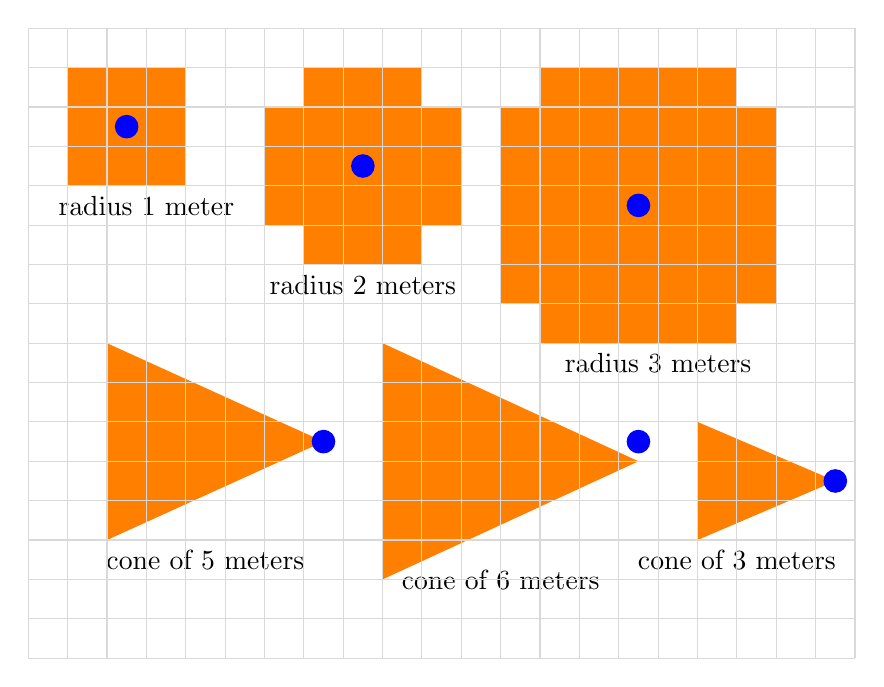
\begin{tikzpicture}[scale=0.5]


\fill[orange] (1,17) rectangle (4,20);
\fill[blue] (2.5,18.5) circle (0.3);
\node at (3,16) [above] {radius 1 meter};

\fill[orange] (6,15) rectangle (11,20);
\fill[white] (5,20) rectangle (6,21);
\fill[white] (6,19) rectangle (7,20); 
\fill[white] (10,15) rectangle (11,16);
\fill[white] (6,15) rectangle (7,16);
\fill[white] (10,19) rectangle (11,20);
\fill[blue] (8.5,17.5) circle (0.3); 
\node at (8.5,14) [above] {radius 2 meters};

\fill[orange] (12,13) rectangle (19,20);
\fill[white] (12,19) rectangle (13,20);
\fill[white] (18,13) rectangle (19,14);
\fill[white] (12,13) rectangle (13,14);
\fill[white] (18,19) rectangle (19,20);
\fill[blue] (15.5,16.5) circle (0.3); 
\node at (16,12) [above] {radius 3 meters};


\fill[orange] (2,8) -- (7.5,10.5) -- (2,13) -- cycle;
\fill[blue] (7.5,10.5) circle (0.3); 
\node at (4.5,7) [above] {cone of 5 meters};


\fill[orange] (17,8) -- (20.5,9.5) -- (17,11) -- cycle;
\fill[blue] (20.5,9.5) circle (0.3); 
\node at (18,7) [above] {cone of 3 meters};

%\fill[orange] (9,7) -- (15.5,10.5) -- (9,13) -- cycle;
%\fill[blue] (15.5,10.5) circle (0.3); 
%\node at (12,6.5) [above] {cono di 6 metri};

\fill[orange] (9,7) -- (15.5,10) -- (9,13) -- cycle;
\fill[blue] (15.5,10.5) circle (0.3); % Blue point on the right tip
\node at (12,6.5) [above] {cone of 6 meters};

% Cube of 3 squares per side
%\fill[orange] (2,2) -- (5,2) -- (5,5) -- (2,5) -- cycle; % Front face
%\fill[orange] (5,2) -- (6,3) -- (6,6) -- (5,5) -- cycle; % Right face
%\fill[orange] (2,5) -- (5,5) -- (6,6) -- (3,6) -- cycle; % Upper face

% Cube of 6 squares per side
%\fill[orange] (8,2) -- (14,2) -- (14,8) -- (8,8) -- cycle; % Front face
%\fill[orange] (14,2) -- (16,4) -- (16,10) -- (14,8) -- cycle; % Right face
%\fill[orange] (8,8) -- (14,8) -- (16,10) -- (10,10) -- cycle; % Upper face

% Draw the base grid (20x15)
\foreach \x in {0,...,20}
\foreach \y in {5,...,20}
\draw[gray!30] (\x,\y) grid (\x+1,\y+1);


\end{tikzpicture}

\medskip

The blue point determines the origin of the spell

\bigskip

\textbf{Examples of enemy reach}

\medskip

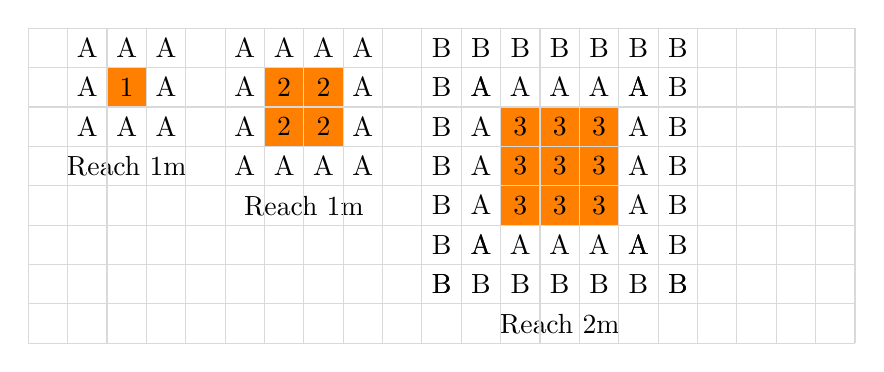
\begin{tikzpicture}[scale=0.5]


\fill[orange] (1,18) rectangle (2,19);
\node at (1.5,18.5) {1}; 

\foreach \x in {-1,...,1} {
\node at (\x+1.5,17.5) {A};
\node at (\x+1.5,19.5) {A};
}

\foreach \y in {18} { \node at (+0.5,\y+0.5) {A};
\node at (2.5,\y+0.5) {A}; }

\node at (1.5,16) [above] {Reach 1m};


% Central 2x2 square with number 2 inside
\fill[orange] (5,17) rectangle (7,19);
\node at (5.5,17.5) {2}; 
\node at (5.5,18.5) {2}; 
\node at (6.5,17.5) {2}; 
\node at (6.5,18.5) {2}; 

% Letters A around the central 2x2 square
\foreach \x in {3,...,6} {
\node at (\x+1.5,19.5) {A}; % Above
\node at (\x+1.5,16.5) {A}; % Below
}
\foreach \y in {9,...,10} {
\node at (4.5,\y+8.5) {A}; % Left
\node at (7.5,\y+8.5) {A}; % Right
}

\node at (6,15) [above] {Reach 1m};


% 3x3 square with number 3 inside, shifted left by 1 square and up by 1 square
\fill[orange] (11,15) rectangle (14,18);
\node at (11.5,17.5) {3}; 
\node at (12.5,17.5) {3}; 
\node at (13.5,17.5) {3}; 

\node at (11.5,16.5) {3}; 
\node at (12.5,16.5) {3}; 
\node at (13.5,16.5) {3}; 

\node at (11.5,15.5) {3}; 
\node at (12.5,15.5) {3}; 
\node at (13.5,15.5) {3}; 

% First frame of squares with letter A
% Above and below the 3x3 square
\foreach \x in {10,...,14} {
\node at (\x+0.5,14.5) {A};
\node at (\x+0.5,18.5) {A};
}

% On the sides of the 3x3 square
\foreach \y in {13,...,17} {
\node at (10.5,\y+1.5) {A};
\node at (14.5,\y+1.5) {A};
}

% Second frame of squares with letter B
% Above and below the first frame
\foreach \x in {9,...,15} {
\node at (\x+0.5,19.5) {B};
\node at (\x+0.5,13.5) {B};
}

% On the sides of the first frame
\foreach \y in {13,...,18} {
\node at (9.5,\y+0.5) {B};
\node at (15.5,\y+0.5) {B};
}
\node at (12.5,12) [above] {Reach 2m};



\foreach \x in {-1,...,19}
\foreach \y in {12,...,19}
\draw[gray!30] (\x,\y) grid (\x+1,\y+1);

\end{tikzpicture}

%\bigskip

%\textbf{Example of Flanking}

%	\begin{tikzpicture}[scale=0.7]
% Disegna il reticolato 4x4
%\foreach \i in {0,...,4} {
%	\draw[thick] (\i,0) -- (\i,4);
%	\draw[thick] (0,\i) -- (4,\i);
%}

% Colora i quadrati 2, 3, 14 e 15 di arancione
%\fill[orange!60, opacity=0.7] (1,3) rectangle (2,4); % quadrato 2
%\fill[orange!60, opacity=0.7] (2,3) rectangle (3,4); % quadrato 3
%\fill[orange!60, opacity=0.7] (1,0) rectangle (2,1); % quadrato 14
%\fill[orange!60, opacity=0.7] (2,0) rectangle (3,1); % quadrato 15

% Traccia linee dritte che attraversano i quadrati
% Linea dal 3 al 14
%\draw[red, ultra thick] (2.5,3.5) -- (1.5,0.5);

% Linea dal 2 al 15
%\draw[blue, ultra thick] (1.5,3.5) -- (2.5,0.5);

% Nuova linea da 4 a 13 (nera)
%\draw[black, ultra thick] (3.5,3.5) -- (0.5,0.5);

% Nuova linea da 1 a 16 (gialla)
%\draw[yellow!80!black, ultra thick] (0.5,3.5) -- (3.5,0.5);

% Numera i quadrati da 1 a 16
%\foreach \i in {0,...,3} {
%	\foreach \j in {0,...,3} {
%		\pgfmathtruncatemacro{\num}{4*(3-\j)+\i+1}
%		\node at (\i+0.5,\j+0.5) {\Large \num};
%	}
%}
%	
%\end{tikzpicture}

%\smallskip

%In this example	Characters at 1-16,2-15,3-14,4-15 are flanking the enemy.

\pagebreak


\noindent



\section{Author and Contributions}

\index[OBSSv2]{Author}

\textbf{Author}: Andres Zanzani - azanzani@gmail.com

\medskip

\noindent\textbf{Contributions}: Federica Angeli



\section{Material for playing}



\index[OBSSv2]{Sheet}\index[OBSSv2]{Manuals}\index[OBSSv2]{Screen}\index[OBSSv2]{About Characters}

\label{scheda-e-manuale}

You are invited to download \textbf{Old Bell School System} from GitHub freely and without constraints except for those expressed in the license.
The main site is \href{https://github.com/buzzqw/TUS}{https://github.com/buzzqw/TUS}

\medskip

* \textbf{OBSS Manual}:
\href{https://github.com/buzzqw/TUS/blob/master/OBSS/OBSSv2.pdf}{OBSSv2-eng.pdf}

https://github.com/buzzqw/TUS/blob/master/OBSS/OBSSv2-eng.pdf

\smallskip

* \textbf{Character Sheet}:
\href{https://github.com/buzzqw/TUS/blob/master/OBSS/OBSS-scheda.pdf}{OBSS-scheda-eng.pdf}

https://github.com/buzzqw/TUS/blob/master/OBSS/OBSS-scheda-eng.pdf

\smallskip

* \textbf{Narrator's Screen}: 
\href{https://github.com/buzzqw/TUS/blob/master/OBSS/screenv2.pdf}{screenv2-eng.pdf}

https://github.com/buzzqw/TUS/blob/master/OBSS/screenv2-eng.pdf

\smallskip

* \textbf{Character Information}:
\href{https://github.com/buzzqw/TUS/blob/master/OBSS/OBSS-schema-arbiter-character-eng.pdf}{OBSS-schema-arbiter-character-eng.pdf}

https://github.com/buzzqw/TUS/blob/master/OBSS/OBSS-schema-arbiter-character-eng.pdf

\smallskip

* \textbf{Changelog, only in italian} \href{https://github.com/buzzqw/TUS/blob/master/OBSS/changelog.md}{changelog.md} 

https://github.com/buzzqw/TUS/blob/master/OBSS/changelog.md

\smallskip

* \textbf{Feedback}

For any feedback or suggestions, please open an issue on GitHub, or send me an email at azanzani@gmail.com% or contact me on the OBSS Telegram group \href{https://t.me/obssgdr}{https://t.me/obssgdr}



\section{Acknowledgments}

\index[OBSSv2]{Acknowledgments}\index[OBSSv2]{DnD SRD}


\begin{changemargin}{0.3cm}{0.3cm}\begin{enfasi}{
\begin{center}
To my friends, to my adventure companions, to all the players who close their eyes and let themselves be guided by imagination into wonderful adventures. (Andres Zanzani)
\end{center}
}\end{enfasi}\end{changemargin}

\medskip

Part of the material is adapted from \href{https://media.wizards.com/2023/downloads/dnd/SRD_CC_v5.1_IT.pdf}{SRD\_CC\_v5.1\_IT.pdf} released by Wizards of the Coast.

Link https://media.wizards.com/2023/downloads/dnd/SRD\_CC\_v5.1\_IT.pdf

\medskip

%Ringrazio \href{https://github.com/ThomasJockin/readexpro}{Readex} ( https://github.com/ThomasJockin/readexpro ) per il font usato. Readex è un font dall'alta leggibilità anche per persone con difficoltà di lettura.

I thank the \href{https://www.brailleinstitute.org/freefont/}{Braille Institute} for the font used. Atkinson Hyperlegible Font is a highly readable font, even for people with reading difficulties.



\section{License}

\hypertarget{Licenza}{}\label{Licenza}

\textbf{Old Bell School System (OBSS)} © 2021 by Andres Zanzani is licensed under \hyperref{https://creativecommons.org/licenses/by-sa/4.0/legalcode}{}{}{CC BY-SA 4.0} 

The images in the manuals are unlicensed or in the public domain. Images marked with \emph{B.I.C.} and the cover were created with Bing Image Creator. If any copyright-protected images are included, please notify us so we can proceed with their removal.

Before any use of OBSS or parts of it, please contact me.

\vspace{0.8cm}

\noindent\begin{minipage}{0.5\textwidth}% adapt widths of minipages to your needs
\includegraphics[keepaspectratio,width=\linewidth]{immagini/CC_BY-SA_icon.svg.png}
\end{minipage}
%
\begin{minipage}{0.5\textwidth}\raggedleft
\large{Powered by} \Huge\LaTeX\ {\normalsize {\&}} \Huge\textbf{GitHub}
\end{minipage}

\vfill

\begin{changemargin}{0.3cm}{0.3cm}\begin{enfasi}{
\begin{center}
And enjoy the game. (Players' Guide to Immortals. Frank Mentzer)
\end{center}
}\end{enfasi}\end{changemargin}

%\vspace{0.5cm}


\thispagestyle{plain}
\begin{center}
\includepdf[pages={1,2},addtotoc={1,section,0,Scheda del Personaggio,incl:first},scale=0.9]{OBSS-scheda-eng.pdf}
%\includepdf[pages={1,2},scale=0.85]{OBSS-scheda.pdf}
\end{center}


%\thispagestyle{plain}
%\begin{center}
%\begin{tikzpicture}[remember picture,overlay]
%\node[anchor=south west,inner sep=0pt] at ($(current page.south west)+(1cm,1cm)$) {
%\includegraphics[scale=0.93]{OBSS-scheda-0.png}
%};
%\end{tikzpicture}
%\end{center}
%\pagebreak
%\thispagestyle{plain}
%\begin{center}
%\begin{tikzpicture}[remember picture,overlay]
%\node[anchor=south west,inner sep=0pt] at ($(current page.south west)+(1cm,1cm)$) {
%\includegraphics[scale=0.93]{OBSS-scheda-1.png}
%};
%\end{tikzpicture}
%\end{center}

\pagebreak




\section{My Options}

\index[OBSSv2]{Le mie Opzioni}

\normalsize

I am also a Narrator, and while I built OBSS based on my preferences, there are some Options that make the game more \emph{unique} that I like to make available to the characters.

At my gaming table, I usually propose these Options, to be decided in Session Zero:

\begin{itemize}[leftmargin=*] \setlength{\itemsep}{0pt}

\item
\hyperlink{successoparziale}{Partial Success} page \pageref{successoparziale}

\item
\hyperlink{varianteiniziativa}{Initiative Variant}, only if I have experienced players. Page \pageref{varianteiniziativa}

\item
Starting with \hyperlink{variantetiricritici}{Critical Roll Variant}. \hyperlink{tirocriticovariante}{Critical Roll Variant}, \hyperlink{OpzionaleAzioniTiroCritico}{Critical Roll Actions}, \hyperlink{varianteattacchimultipli}{Multiple Attacks Variant} are up to the player whether to use them or not. Page \pageref{tirocriticovariante}, page \pageref{OpzionaleAzioniTiroCritico}, page \pageref{variantetiricritici} and page \pageref{varianteattacchimultipli}. These are Options suggested for experienced players.

\item \hyperlink{elencotalentiarmi}{Optional - List of Weapon Maneuvers} (page \pageref{elencotalentiarmi}) to make fumbling less \emph{boring}...

%\item
%\hyperlink{lunicaregola}{L'Unica Regola} la uso se sono Narratore di un gruppo di principianti. Pag. \pageref{lunicaregola}

\item 
\hyperlink{One Belief}{One Belief} or \hyperlink{abilitadilista}{List Feats}, at the player's choice.

\item
\hyperlink{componenticomeofferta}{Components as Offerings} for a personal, different, and unique magic, always tied to the character. Page \pageref{componenticomeofferta}

\item
\hyperlink{abilitaiconiche}{Iconic Feats} for long campaigns. Page \pageref{abilitaiconiche}

\item
\hyperlink{droghe}{Drugs} \textbf{NO}. Only for groups composed of mentally mature and adult people. Page \pageref{droghe}

\item
\textbf{No to using a timer on Lights}: if your adventures are not set in dungeons or you want a more streamlined management, don't manage light duration in real-time.

\end{itemize}


\vfill
{\small

\begin{multicols}{2}

\subsubsection*{Notes}

For me, OBSS should be played straightforwardly, without overthinking or making overly cerebral plans. OBSS is not designed to kill characters, but at the same time, it doesn't facilitate their survival; it's up to the Narrator to decide how to play. The key to the game lies in the Narrator, the players' style, and the group's interest. OBSS aims to provide the framework and tools to play the adventure.

Try to emphasize scenes, be theatrical in your descriptions, and remove the veneer of clean, politically correct gameplay. It's always your world, your table, and your game; try to provide the immersion that has been somewhat lost in more modern systems.
When there's combat, make it feel like combat! You should hear the clanging of weapons, the clash on armor, the ozone in the air caused by lightning, the crackling burns of fireballs. Let players appreciate the possibilities offered by the system and enjoy finding the best way to make a check.

Choose whether the characters are rogues just trying to survive and accumulate treasures or give a more classic or epic touch to the adventure. OBSS works with both choices, especially when using some Options over others.

Create the group, and I don't just mean as a set of characters, but also as a set of players. A group where people respect and trust each other (hopefully...). Build adventures that involve everyone, where everyone can contribute. There may be adventures more "tailored" around one character, but this \textbf{must not} exclude others from participating in the broadest sense of the word. Don't let the session be a monologue between you and a single player.
Take advantage of every adventure to help characters get to know each other; nothing unites more than the fear of death!

Once you've formed the group, which might take time, exploit personal stories, clues, and hypotheses created by the players to shape situations and events. Like a heavy flywheel that rotates, this will continue to create situations, adventures, and new plots to follow.

There might be difficulties in creating the group, unfortunately. Try to talk to the player causing problems. Try to understand if it's their character that doesn't "work" with the group or if the player hasn't fully understood the group dynamics.

This is why I always suggest doing a so-called \hyperlink{sessionezero}{Session Zero} (page \pageref{sessionezero}), where as the Narrator you will outline the main pillars of the adventure, what you expect from the characters, and what basic and moral rules to follow. There's nothing worse than a group of disconnected characters where everyone wants to do something different and isn't interested in the \emph{common goal}.

It's very important to understand what players like; each person and group wants a certain style of play, and it's right to try to accommodate them. If the group wants political adventures or romantic dramas, try to let them find satisfaction during the adventure. If they prefer more combat, then don't skimp on encounters as long as they're consistent with the adventure itself.

Make it clear that you need to function as a group of players and characters to play at your best, have fun together, and have a better chance of survival. No player should be above others; only the Narrator has the final word.

Finally, always be fair, for better or worse. There will be less fortunate sessions and others where the dice will find the right path, where a brilliant idea will save the group. Don't be the Narrator who \textbf{always and invariably} saves the characters. An occasional help is okay, especially in a more unfortunate session, but respect the characters' choices and the outcome of the dice. Remember that players have Fate Points to use, unlike the poor monsters!

Personally, I roll all dice in front of the players.

The \textbf{Narrator must not steal the scene} from the characters but build the environment, dramas, and passions around them. There's nothing more annoying than a Narrator with protagonist tendencies, whether in handling NPCs or imposing choices and scenes.

And finally, an obvious point: \textbf{have fun}, all of you \textbf{strive} to make the session have that mix of tension, fun, and satisfaction. You are people who want to play, have fun, and be together; never forget that.
\end{multicols}}

\pagebreak


\begin{multicols}{4}
	{\small\printindex[OBSSv2]}
\end{multicols}

\TotalBox{OBSSv2} \pagebreak

\begin{multicols}{3}
{\small\printindex[Table]}
\end{multicols}

\vfill

\TotalBox{Table}\pagebreak

\begin{multicols}{3}
{\small\printindex[Spell]}
\end{multicols}

%\immediate\write18{./contaspell.sh > contaspell.txt}
%\immediate\openin\myscriptresult=./contaspell.txt
%\read\myscriptresult to \ScriptResult
%\immediate\closein\myscriptresult

\vfill

%Totale elementi in questo indice \ScriptResult

\TotalBox{Spell}\pagebreak



\begin{multicols}{3}
	{\small\printindex[MagicItems]}
\end{multicols}


%{\scriptsize\printindex[OggettiMagici]}


%\immediate\write18{./contaomagici.sh > contaomagici.txt}
%\immediate\openin\myscriptresult=./contaomagici.txt
%\read\myscriptresult to \ScriptResult
%\immediate\closein\myscriptresult

\vfill

%Totale elementi in questo indice \ScriptResult

\TotalBox{MagicItems}\pagebreak


\begin{multicols}{3}
	{\small\printindex[Feat]}
\end{multicols}

\vfill

\TotalBox{Feat}\pagebreak


\begin{multicols}{3}
	{\small\printindex[Monster]}
\end{multicols}

\vfill

\TotalBox{Monster}

%Totale elementi in questo indice \ScriptResult

%\immediate\write18{./contamostri.sh > contamostri.txt}
%\immediate\openin\myscriptresult=./contamostri.txt
%\read\myscriptresult to \ScriptResult
%\immediate\closein\myscriptresult

\end{document}
